\documentclass{book}
\usepackage[a4paper,top=2.5cm,bottom=2.5cm,left=2.5cm,right=2.5cm]{geometry}
\usepackage{makeidx}
\usepackage{natbib}
\usepackage{graphicx}
\usepackage{multicol}
\usepackage{float}
\usepackage{listings}
\usepackage{color}
\usepackage{ifthen}
\usepackage[table]{xcolor}
\usepackage{textcomp}
\usepackage{alltt}
\usepackage{ifpdf}
\ifpdf
\usepackage[pdftex,
            pagebackref=true,
            colorlinks=true,
            linkcolor=blue,
            unicode
           ]{hyperref}
\else
\usepackage[ps2pdf,
            pagebackref=true,
            colorlinks=true,
            linkcolor=blue,
            unicode
           ]{hyperref}
\usepackage{pspicture}
\fi
\usepackage[utf8]{inputenc}
\usepackage{mathptmx}
\usepackage[scaled=.90]{helvet}
\usepackage{courier}
\usepackage{sectsty}
\usepackage{amssymb}
\usepackage[titles]{tocloft}
\usepackage{doxygen}
\lstset{language=C++,inputencoding=utf8,basicstyle=\footnotesize,breaklines=true,breakatwhitespace=true,tabsize=4,numbers=left }
\makeindex
\setcounter{tocdepth}{3}
\renewcommand{\footrulewidth}{0.4pt}
\renewcommand{\familydefault}{\sfdefault}
\hfuzz=15pt
\setlength{\emergencystretch}{15pt}
\hbadness=750
\tolerance=750
\begin{document}
\hypersetup{pageanchor=false,citecolor=blue}
\begin{titlepage}
\vspace*{7cm}
\begin{center}
{\Large Kameleon-\/\-Plus \\[1ex]\large 0.\-3.\-2 }\\
\vspace*{1cm}
{\large Generated by Doxygen 1.8.3}\\
\vspace*{0.5cm}
{\small Wed Apr 16 2014 18:34:48}\\
\end{center}
\end{titlepage}
\clearemptydoublepage
\pagenumbering{roman}
\tableofcontents
\clearemptydoublepage
\pagenumbering{arabic}
\hypersetup{pageanchor=true,citecolor=blue}
\chapter{Kameleon Interpolator}
\label{index}\hypertarget{index}{}The Kameleon-\/\-Interpolator library is a C++ library that provides classes to access and interpolate from data files produced by multiple space weather products. It currently supports the output from the following products\-:
\begin{DoxyItemize}
\item Open\-G\-G\-C\-M
\item B\-A\-T\-S\-R\-U\-S (Global M\-H\-D) and the B\-A\-T\-S\-R\-U\-S component of S\-W\-M\-F
\item Ionospheric component of S\-W\-M\-F
\item E\-N\-L\-I\-L
\item M\-A\-S
\item C\-T\-I\-P
\item A\-D\-A\-P\-T3\-D
\end{DoxyItemize}

Java, C, and Fortran compatible interfaces are provided through the use of the wrapper headers and code (ccmc/wrappers/$\ast$).\hypertarget{index_Purpose}{}\section{Purpose}\label{index_Purpose}
The purpose of this library is to provide easy access and interpolation methods for multiple space weather simulation model datasets, to provide access to derived variables, and to calculate fieldlines using any of the model vector field variables. Derived variables are those that can be calculated from the base variables provided by the native data files.\hypertarget{index_Examples}{}\section{Example code}\label{index_Examples}
\hypertarget{index_License}{}\section{License}\label{index_License}

\chapter{Module Index}
\section{Modules}
Here is a list of all modules\-:\begin{DoxyCompactList}
\item \contentsline{section}{nanoflann C++ library for A\-N\-N}{\pageref{group__nanoflann__grp}}{}
\begin{DoxyCompactList}
\item \contentsline{section}{Result set classes}{\pageref{group__result__sets__grp}}{}
\item \contentsline{section}{Load/save auxiliary functions}{\pageref{group__loadsave__grp}}{}
\item \contentsline{section}{Metric (distance) classes}{\pageref{group__metric__grp}}{}
\item \contentsline{section}{Parameter structs}{\pageref{group__param__grp}}{}
\item \contentsline{section}{Memory allocation}{\pageref{group__memalloc__grp}}{}
\item \contentsline{section}{K\-D-\/tree classes and adaptors}{\pageref{group__kdtrees__grp}}{}
\end{DoxyCompactList}
\end{DoxyCompactList}

\chapter{Namespace Index}
\section{Namespace List}
Here is a list of all namespaces with brief descriptions\-:\begin{DoxyCompactList}
\item\contentsline{section}{\hyperlink{namespaceccmc}{ccmc} \\*Namespace for the Community Coordinated Modeling Center code }{\pageref{namespaceccmc}}{}
\item\contentsline{section}{\hyperlink{namespaceccmc_1_1constants}{ccmc\-::constants} }{\pageref{namespaceccmc_1_1constants}}{}
\item\contentsline{section}{\hyperlink{namespaceccmc_1_1defaults}{ccmc\-::defaults} }{\pageref{namespaceccmc_1_1defaults}}{}
\item\contentsline{section}{\hyperlink{namespaceccmc_1_1strings}{ccmc\-::strings} }{\pageref{namespaceccmc_1_1strings}}{}
\item\contentsline{section}{\hyperlink{namespaceccmc_1_1strings_1_1attributes}{ccmc\-::strings\-::attributes} }{\pageref{namespaceccmc_1_1strings_1_1attributes}}{}
\item\contentsline{section}{\hyperlink{namespaceccmc_1_1strings_1_1models}{ccmc\-::strings\-::models} }{\pageref{namespaceccmc_1_1strings_1_1models}}{}
\item\contentsline{section}{\hyperlink{namespaceccmc_1_1strings_1_1variables}{ccmc\-::strings\-::variables} }{\pageref{namespaceccmc_1_1strings_1_1variables}}{}
\end{DoxyCompactList}

\chapter{Hierarchical Index}
\section{Class Hierarchy}
This inheritance list is sorted roughly, but not completely, alphabetically\-:\begin{DoxyCompactList}
\item \contentsline{section}{ccmc\-:\-:Attribute}{\pageref{classccmc_1_1_attribute}}{}
\item \contentsline{section}{ccmc\-:\-:Fieldline}{\pageref{classccmc_1_1_fieldline}}{}
\item \contentsline{section}{ccmc\-:\-:File\-Reader}{\pageref{classccmc_1_1_file_reader}}{}
\begin{DoxyCompactList}
\item \contentsline{section}{ccmc\-:\-:C\-D\-F\-File\-Reader}{\pageref{classccmc_1_1_c_d_f_file_reader}}{}
\end{DoxyCompactList}
\item \contentsline{section}{ccmc\-:\-:General\-File\-Reader}{\pageref{classccmc_1_1_general_file_reader}}{}
\begin{DoxyCompactList}
\item \contentsline{section}{ccmc\-:\-:Model}{\pageref{classccmc_1_1_model}}{}
\begin{DoxyCompactList}
\item \contentsline{section}{ccmc\-:\-:Adapt3\-D}{\pageref{classccmc_1_1_adapt3_d}}{}
\item \contentsline{section}{ccmc\-:\-:B\-A\-T\-S\-R\-U\-S}{\pageref{classccmc_1_1_b_a_t_s_r_u_s}}{}
\item \contentsline{section}{ccmc\-:\-:C\-T\-I\-P}{\pageref{classccmc_1_1_c_t_i_p}}{}
\item \contentsline{section}{ccmc\-:\-:E\-N\-L\-I\-L}{\pageref{classccmc_1_1_e_n_l_i_l}}{}
\item \contentsline{section}{ccmc\-:\-:Magnetogram}{\pageref{classccmc_1_1_magnetogram}}{}
\item \contentsline{section}{ccmc\-:\-:M\-A\-S}{\pageref{classccmc_1_1_m_a_s}}{}
\item \contentsline{section}{ccmc\-:\-:Open\-G\-G\-C\-M}{\pageref{classccmc_1_1_open_g_g_c_m}}{}
\item \contentsline{section}{ccmc\-:\-:S\-W\-M\-F\-Iono}{\pageref{classccmc_1_1_s_w_m_f_iono}}{}
\end{DoxyCompactList}
\end{DoxyCompactList}
\item \contentsline{section}{ccmc\-:\-:Interpolator}{\pageref{classccmc_1_1_interpolator}}{}
\begin{DoxyCompactList}
\item \contentsline{section}{ccmc\-:\-:Adapt3\-D\-Interpolator}{\pageref{classccmc_1_1_adapt3_d_interpolator}}{}
\item \contentsline{section}{ccmc\-:\-:B\-A\-T\-S\-R\-U\-S\-Interpolator}{\pageref{classccmc_1_1_b_a_t_s_r_u_s_interpolator}}{}
\item \contentsline{section}{ccmc\-:\-:E\-N\-L\-I\-L\-Interpolator}{\pageref{classccmc_1_1_e_n_l_i_l_interpolator}}{}
\item \contentsline{section}{ccmc\-:\-:Kameleon\-Interpolator}{\pageref{classccmc_1_1_kameleon_interpolator}}{}
\item \contentsline{section}{ccmc\-:\-:Magnetogram\-Interpolator}{\pageref{classccmc_1_1_magnetogram_interpolator}}{}
\item \contentsline{section}{ccmc\-:\-:M\-A\-S\-Interpolator}{\pageref{classccmc_1_1_m_a_s_interpolator}}{}
\item \contentsline{section}{ccmc\-:\-:Open\-G\-G\-C\-M\-Interpolator}{\pageref{classccmc_1_1_open_g_g_c_m_interpolator}}{}
\item \contentsline{section}{ccmc\-:\-:S\-W\-M\-F\-Iono\-Interpolator}{\pageref{classccmc_1_1_s_w_m_f_iono_interpolator}}{}
\end{DoxyCompactList}
\item \contentsline{section}{ccmc\-:\-:Kameleon}{\pageref{classccmc_1_1_kameleon}}{}
\item \contentsline{section}{Kameleon}{\pageref{class_kameleon}}{}
\item \contentsline{section}{ccmc\-:\-:Math}{\pageref{classccmc_1_1_math}}{}
\item \contentsline{section}{ccmc\-:\-:Point$<$ T $>$}{\pageref{classccmc_1_1_point}}{}
\begin{DoxyCompactList}
\item \contentsline{section}{ccmc\-:\-:Vector$<$ T $>$}{\pageref{classccmc_1_1_vector}}{}
\end{DoxyCompactList}
\item \contentsline{section}{ccmc\-:\-:Point3f}{\pageref{classccmc_1_1_point3f}}{}
\item \contentsline{section}{ccmc\-:\-:Position}{\pageref{structccmc_1_1_position}}{}
\item \contentsline{section}{ccmc\-:\-:Smart\-Grid\-Search\-Values}{\pageref{structccmc_1_1_smart_grid_search_values}}{}
\item \contentsline{section}{ccmc\-:\-:Time}{\pageref{classccmc_1_1_time}}{}
\item \contentsline{section}{ccmc\-:\-:Tracer}{\pageref{classccmc_1_1_tracer}}{}
\item \contentsline{section}{ccmc\-:\-:Utils$<$ T $>$}{\pageref{classccmc_1_1_utils}}{}
\end{DoxyCompactList}

\chapter{Class Index}
\section{Class List}
Here are the classes, structs, unions and interfaces with brief descriptions\-:\begin{DoxyCompactList}
\item\contentsline{section}{\hyperlink{classccmc_1_1_adapt3_d}{ccmc\-::\-Adapt3\-D} \\*T\-O\-D\-O\-: brief description of \hyperlink{classccmc_1_1_adapt3_d}{Adapt3\-D} class }{\pageref{classccmc_1_1_adapt3_d}}{}
\item\contentsline{section}{\hyperlink{classccmc_1_1_adapt3_d_interpolator}{ccmc\-::\-Adapt3\-D\-Interpolator} \\*T\-O\-D\-O\-: brief description of \hyperlink{classccmc_1_1_b_a_t_s_r_u_s_interpolator}{B\-A\-T\-S\-R\-U\-S\-Interpolator} class }{\pageref{classccmc_1_1_adapt3_d_interpolator}}{}
\item\contentsline{section}{\hyperlink{classccmc_1_1_attribute}{ccmc\-::\-Attribute} \\*T\-O\-D\-O\-: brief description of \hyperlink{classccmc_1_1_attribute}{Attribute} class }{\pageref{classccmc_1_1_attribute}}{}
\item\contentsline{section}{\hyperlink{classccmc_1_1_axis_polyhedron}{ccmc\-::\-Axis\-Polyhedron$<$ T $>$} }{\pageref{classccmc_1_1_axis_polyhedron}}{}
\item\contentsline{section}{\hyperlink{classccmc_1_1_b_a_t_s_r_u_s}{ccmc\-::\-B\-A\-T\-S\-R\-U\-S} \\*T\-O\-D\-O\-: brief description of \hyperlink{classccmc_1_1_b_a_t_s_r_u_s}{B\-A\-T\-S\-R\-U\-S} class }{\pageref{classccmc_1_1_b_a_t_s_r_u_s}}{}
\item\contentsline{section}{\hyperlink{classccmc_1_1_b_a_t_s_r_u_s_interpolator}{ccmc\-::\-B\-A\-T\-S\-R\-U\-S\-Interpolator} \\*T\-O\-D\-O\-: brief description of \hyperlink{classccmc_1_1_b_a_t_s_r_u_s_interpolator}{B\-A\-T\-S\-R\-U\-S\-Interpolator} class }{\pageref{classccmc_1_1_b_a_t_s_r_u_s_interpolator}}{}
\item\contentsline{section}{\hyperlink{structnanoflann_1_1_k_d_tree_single_index_adaptor_1_1_branch_struct}{nanoflann\-::\-K\-D\-Tree\-Single\-Index\-Adaptor$<$ Distance, Dataset\-Adaptor, D\-I\-M, Index\-Type $>$\-::\-Branch\-Struct$<$ T, Distance\-Type $>$} }{\pageref{structnanoflann_1_1_k_d_tree_single_index_adaptor_1_1_branch_struct}}{}
\item\contentsline{section}{\hyperlink{classccmc_1_1_c_d_f_file_reader}{ccmc\-::\-C\-D\-F\-File\-Reader} }{\pageref{classccmc_1_1_c_d_f_file_reader}}{}
\item\contentsline{section}{\hyperlink{classccmc_1_1_c_t_i_p}{ccmc\-::\-C\-T\-I\-P} \\*T\-O\-D\-O\-: Brief description of \hyperlink{classccmc_1_1_c_t_i_p}{C\-T\-I\-P} class }{\pageref{classccmc_1_1_c_t_i_p}}{}
\item\contentsline{section}{\hyperlink{classccmc_1_1_e_n_l_i_l}{ccmc\-::\-E\-N\-L\-I\-L} \\*T\-O\-D\-O\-: Brief description of \hyperlink{classccmc_1_1_e_n_l_i_l}{E\-N\-L\-I\-L} class }{\pageref{classccmc_1_1_e_n_l_i_l}}{}
\item\contentsline{section}{\hyperlink{classccmc_1_1_e_n_l_i_l_interpolator}{ccmc\-::\-E\-N\-L\-I\-L\-Interpolator} \\*T\-O\-D\-O\-: Brief description of \hyperlink{classccmc_1_1_e_n_l_i_l_interpolator}{E\-N\-L\-I\-L\-Interpolator} class }{\pageref{classccmc_1_1_e_n_l_i_l_interpolator}}{}
\item\contentsline{section}{\hyperlink{classccmc_1_1_fieldline}{ccmc\-::\-Fieldline} }{\pageref{classccmc_1_1_fieldline}}{}
\item\contentsline{section}{\hyperlink{classccmc_1_1_file_reader}{ccmc\-::\-File\-Reader} \\*T\-O\-D\-O\-: Brief description of \hyperlink{classccmc_1_1_file_reader}{File\-Reader} class }{\pageref{classccmc_1_1_file_reader}}{}
\item\contentsline{section}{\hyperlink{classccmc_1_1_general_file_reader}{ccmc\-::\-General\-File\-Reader} }{\pageref{classccmc_1_1_general_file_reader}}{}
\item\contentsline{section}{\hyperlink{classccmc_1_1_grid_polyhedron}{ccmc\-::\-Grid\-Polyhedron$<$ T $>$} }{\pageref{classccmc_1_1_grid_polyhedron}}{}
\item\contentsline{section}{\hyperlink{structnanoflann_1_1_index_dist___sorter}{nanoflann\-::\-Index\-Dist\-\_\-\-Sorter} }{\pageref{structnanoflann_1_1_index_dist___sorter}}{}
\item\contentsline{section}{\hyperlink{classccmc_1_1_interpolator}{ccmc\-::\-Interpolator} \\*T\-O\-D\-O\-: Brief description of \hyperlink{classccmc_1_1_interpolator}{Interpolator} class }{\pageref{classccmc_1_1_interpolator}}{}
\item\contentsline{section}{\hyperlink{structnanoflann_1_1_k_d_tree_single_index_adaptor_1_1_interval}{nanoflann\-::\-K\-D\-Tree\-Single\-Index\-Adaptor$<$ Distance, Dataset\-Adaptor, D\-I\-M, Index\-Type $>$\-::\-Interval} }{\pageref{structnanoflann_1_1_k_d_tree_single_index_adaptor_1_1_interval}}{}
\item\contentsline{section}{\hyperlink{classccmc_1_1_i_poly}{ccmc\-::\-I\-Poly$<$ T $>$} }{\pageref{classccmc_1_1_i_poly}}{}
\item\contentsline{section}{\hyperlink{classccmc_1_1_j_poly}{ccmc\-::\-J\-Poly$<$ T $>$} }{\pageref{classccmc_1_1_j_poly}}{}
\item\contentsline{section}{\hyperlink{classccmc_1_1_kameleon_interpolator}{ccmc\-::\-Kameleon\-Interpolator} \\*T\-O\-D\-O\-: Brief description of \hyperlink{classccmc_1_1_kameleon_interpolator}{Kameleon\-Interpolator} class }{\pageref{classccmc_1_1_kameleon_interpolator}}{}
\item\contentsline{section}{\hyperlink{structnanoflann_1_1_k_d_tree_eigen_matrix_adaptor}{nanoflann\-::\-K\-D\-Tree\-Eigen\-Matrix\-Adaptor$<$ Matrix\-Type, D\-I\-M, Distance, Index\-Type $>$} }{\pageref{structnanoflann_1_1_k_d_tree_eigen_matrix_adaptor}}{}
\item\contentsline{section}{\hyperlink{classnanoflann_1_1_k_d_tree_single_index_adaptor}{nanoflann\-::\-K\-D\-Tree\-Single\-Index\-Adaptor$<$ Distance, Dataset\-Adaptor, D\-I\-M, Index\-Type $>$} }{\pageref{classnanoflann_1_1_k_d_tree_single_index_adaptor}}{}
\item\contentsline{section}{\hyperlink{structnanoflann_1_1_k_d_tree_single_index_adaptor_params}{nanoflann\-::\-K\-D\-Tree\-Single\-Index\-Adaptor\-Params} }{\pageref{structnanoflann_1_1_k_d_tree_single_index_adaptor_params}}{}
\item\contentsline{section}{\hyperlink{classnanoflann_1_1_k_n_n_result_set}{nanoflann\-::\-K\-N\-N\-Result\-Set$<$ Distance\-Type, Index\-Type, Count\-Type $>$} }{\pageref{classnanoflann_1_1_k_n_n_result_set}}{}
\item\contentsline{section}{\hyperlink{structnanoflann_1_1_l1___adaptor}{nanoflann\-::\-L1\-\_\-\-Adaptor$<$ T, Data\-Source, \-\_\-\-Distance\-Type $>$} }{\pageref{structnanoflann_1_1_l1___adaptor}}{}
\item\contentsline{section}{\hyperlink{structnanoflann_1_1_l2___adaptor}{nanoflann\-::\-L2\-\_\-\-Adaptor$<$ T, Data\-Source, \-\_\-\-Distance\-Type $>$} }{\pageref{structnanoflann_1_1_l2___adaptor}}{}
\item\contentsline{section}{\hyperlink{structnanoflann_1_1_l2___simple___adaptor}{nanoflann\-::\-L2\-\_\-\-Simple\-\_\-\-Adaptor$<$ T, Data\-Source, \-\_\-\-Distance\-Type $>$} }{\pageref{structnanoflann_1_1_l2___simple___adaptor}}{}
\item\contentsline{section}{\hyperlink{classccmc_1_1_l_f_m}{ccmc\-::\-L\-F\-M} \\*T\-O\-D\-O\-: Brief description of \hyperlink{classccmc_1_1_l_f_m}{L\-F\-M} class }{\pageref{classccmc_1_1_l_f_m}}{}
\item\contentsline{section}{\hyperlink{classccmc_1_1_l_f_m_interpolator}{ccmc\-::\-L\-F\-M\-Interpolator} \\*T\-O\-D\-O\-: Brief description of \hyperlink{classccmc_1_1_l_f_m_interpolator}{L\-F\-M\-Interpolator} class }{\pageref{classccmc_1_1_l_f_m_interpolator}}{}
\item\contentsline{section}{\hyperlink{classccmc_1_1_magnetogram}{ccmc\-::\-Magnetogram} \\*T\-O\-D\-O\-: Brief description of \hyperlink{classccmc_1_1_magnetogram}{Magnetogram} class }{\pageref{classccmc_1_1_magnetogram}}{}
\item\contentsline{section}{\hyperlink{classccmc_1_1_magnetogram_interpolator}{ccmc\-::\-Magnetogram\-Interpolator} \\*T\-O\-D\-O\-: Brief description of \hyperlink{classccmc_1_1_magnetogram_interpolator}{Magnetogram\-Interpolator} class }{\pageref{classccmc_1_1_magnetogram_interpolator}}{}
\item\contentsline{section}{\hyperlink{classccmc_1_1_m_a_s}{ccmc\-::\-M\-A\-S} \\*T\-O\-D\-O\-: Brief description of \hyperlink{classccmc_1_1_m_a_s}{M\-A\-S} class }{\pageref{classccmc_1_1_m_a_s}}{}
\item\contentsline{section}{\hyperlink{classccmc_1_1_m_a_s_interpolator}{ccmc\-::\-M\-A\-S\-Interpolator} \\*T\-O\-D\-O\-: Brief description of \hyperlink{classccmc_1_1_m_a_s_interpolator}{M\-A\-S\-Interpolator} class }{\pageref{classccmc_1_1_m_a_s_interpolator}}{}
\item\contentsline{section}{\hyperlink{classccmc_1_1_math}{ccmc\-::\-Math} }{\pageref{classccmc_1_1_math}}{}
\item\contentsline{section}{\hyperlink{structnanoflann_1_1metric___l1}{nanoflann\-::metric\-\_\-\-L1} }{\pageref{structnanoflann_1_1metric___l1}}{}
\item\contentsline{section}{\hyperlink{structnanoflann_1_1metric___l2}{nanoflann\-::metric\-\_\-\-L2} }{\pageref{structnanoflann_1_1metric___l2}}{}
\item\contentsline{section}{\hyperlink{structnanoflann_1_1metric___l2___simple}{nanoflann\-::metric\-\_\-\-L2\-\_\-\-Simple} }{\pageref{structnanoflann_1_1metric___l2___simple}}{}
\item\contentsline{section}{\hyperlink{classccmc_1_1_model}{ccmc\-::\-Model} \\*T\-O\-D\-O\-: Brief description of \hyperlink{classccmc_1_1_model}{Model} class }{\pageref{classccmc_1_1_model}}{}
\item\contentsline{section}{\hyperlink{class_nano_kd_tree}{Nano\-Kd\-Tree$<$ num\-\_\-t $>$} }{\pageref{class_nano_kd_tree}}{}
\item\contentsline{section}{\hyperlink{structnanoflann_1_1_k_d_tree_single_index_adaptor_1_1_node}{nanoflann\-::\-K\-D\-Tree\-Single\-Index\-Adaptor$<$ Distance, Dataset\-Adaptor, D\-I\-M, Index\-Type $>$\-::\-Node} }{\pageref{structnanoflann_1_1_k_d_tree_single_index_adaptor_1_1_node}}{}
\item\contentsline{section}{\hyperlink{classccmc_1_1_open_g_g_c_m}{ccmc\-::\-Open\-G\-G\-C\-M} \\*T\-O\-D\-O\-: Brief description of \hyperlink{classccmc_1_1_open_g_g_c_m}{Open\-G\-G\-C\-M} class }{\pageref{classccmc_1_1_open_g_g_c_m}}{}
\item\contentsline{section}{\hyperlink{classccmc_1_1_open_g_g_c_m_interpolator}{ccmc\-::\-Open\-G\-G\-C\-M\-Interpolator} \\*T\-O\-D\-O\-: Brief description of \hyperlink{classccmc_1_1_open_g_g_c_m_interpolator}{Open\-G\-G\-C\-M\-Interpolator} class }{\pageref{classccmc_1_1_open_g_g_c_m_interpolator}}{}
\item\contentsline{section}{\hyperlink{struct_point_cloud_1_1_point}{Point\-Cloud$<$ T $>$\-::\-Point} }{\pageref{struct_point_cloud_1_1_point}}{}
\item\contentsline{section}{\hyperlink{classccmc_1_1_point}{ccmc\-::\-Point$<$ T $>$} \\*T\-O\-D\-O\-: Brief description of \hyperlink{classccmc_1_1_point}{Point} class }{\pageref{classccmc_1_1_point}}{}
\item\contentsline{section}{\hyperlink{classccmc_1_1_point3f}{ccmc\-::\-Point3f} }{\pageref{classccmc_1_1_point3f}}{}
\item\contentsline{section}{\hyperlink{struct_point_cloud}{Point\-Cloud$<$ T $>$} }{\pageref{struct_point_cloud}}{}
\item\contentsline{section}{\hyperlink{classccmc_1_1_polyhedron}{ccmc\-::\-Polyhedron$<$ T $>$} }{\pageref{classccmc_1_1_polyhedron}}{}
\item\contentsline{section}{\hyperlink{classnanoflann_1_1_pooled_allocator}{nanoflann\-::\-Pooled\-Allocator} }{\pageref{classnanoflann_1_1_pooled_allocator}}{}
\item\contentsline{section}{\hyperlink{classnanoflann_1_1_radius_result_set}{nanoflann\-::\-Radius\-Result\-Set$<$ Distance\-Type, Index\-Type $>$} }{\pageref{classnanoflann_1_1_radius_result_set}}{}
\item\contentsline{section}{\hyperlink{structnanoflann_1_1_search_params}{nanoflann\-::\-Search\-Params} }{\pageref{structnanoflann_1_1_search_params}}{}
\item\contentsline{section}{\hyperlink{structccmc_1_1_smart_grid_search_values}{ccmc\-::\-Smart\-Grid\-Search\-Values} }{\pageref{structccmc_1_1_smart_grid_search_values}}{}
\item\contentsline{section}{\hyperlink{classccmc_1_1_s_w_m_f_iono}{ccmc\-::\-S\-W\-M\-F\-Iono} }{\pageref{classccmc_1_1_s_w_m_f_iono}}{}
\item\contentsline{section}{\hyperlink{classccmc_1_1_s_w_m_f_iono_interpolator}{ccmc\-::\-S\-W\-M\-F\-Iono\-Interpolator} }{\pageref{classccmc_1_1_s_w_m_f_iono_interpolator}}{}
\item\contentsline{section}{\hyperlink{classccmc_1_1_time}{ccmc\-::\-Time} }{\pageref{classccmc_1_1_time}}{}
\item\contentsline{section}{\hyperlink{classccmc_1_1_time_interpolator}{ccmc\-::\-Time\-Interpolator} }{\pageref{classccmc_1_1_time_interpolator}}{}
\item\contentsline{section}{\hyperlink{classccmc_1_1_tracer}{ccmc\-::\-Tracer} \\*T\-O\-D\-O\-: Brief description }{\pageref{classccmc_1_1_tracer}}{}
\item\contentsline{section}{\hyperlink{structnanoflann_1_1metric___l1_1_1traits}{nanoflann\-::metric\-\_\-\-L1\-::traits$<$ T, Data\-Source $>$} }{\pageref{structnanoflann_1_1metric___l1_1_1traits}}{}
\item\contentsline{section}{\hyperlink{structnanoflann_1_1metric___l2_1_1traits}{nanoflann\-::metric\-\_\-\-L2\-::traits$<$ T, Data\-Source $>$} }{\pageref{structnanoflann_1_1metric___l2_1_1traits}}{}
\item\contentsline{section}{\hyperlink{structnanoflann_1_1metric___l2___simple_1_1traits}{nanoflann\-::metric\-\_\-\-L2\-\_\-\-Simple\-::traits$<$ T, Data\-Source $>$} }{\pageref{structnanoflann_1_1metric___l2___simple_1_1traits}}{}
\item\contentsline{section}{\hyperlink{classccmc_1_1_utils}{ccmc\-::\-Utils$<$ T $>$} }{\pageref{classccmc_1_1_utils}}{}
\item\contentsline{section}{\hyperlink{classccmc_1_1_vector}{ccmc\-::\-Vector$<$ T $>$} }{\pageref{classccmc_1_1_vector}}{}
\end{DoxyCompactList}

\chapter{File Index}
\section{File List}
Here is a list of all files with brief descriptions\-:\begin{DoxyCompactList}
\item\contentsline{section}{/\-Users/apembrok/git/ccmc-\/software/kameleon-\/plus/trunk/kameleon-\/plus-\/working/src/ccmc/\hyperlink{_adapt3_d_8cpp}{Adapt3\-D.\-cpp} }{\pageref{_adapt3_d_8cpp}}{}
\item\contentsline{section}{/\-Users/apembrok/git/ccmc-\/software/kameleon-\/plus/trunk/kameleon-\/plus-\/working/src/ccmc/\hyperlink{_adapt3_d_8h}{Adapt3\-D.\-h} }{\pageref{_adapt3_d_8h}}{}
\item\contentsline{section}{/\-Users/apembrok/git/ccmc-\/software/kameleon-\/plus/trunk/kameleon-\/plus-\/working/src/ccmc/\hyperlink{_adapt3_d_interpolator_8cpp}{Adapt3\-D\-Interpolator.\-cpp} }{\pageref{_adapt3_d_interpolator_8cpp}}{}
\item\contentsline{section}{/\-Users/apembrok/git/ccmc-\/software/kameleon-\/plus/trunk/kameleon-\/plus-\/working/src/ccmc/\hyperlink{_adapt3_d_interpolator_8h}{Adapt3\-D\-Interpolator.\-h} }{\pageref{_adapt3_d_interpolator_8h}}{}
\item\contentsline{section}{/\-Users/apembrok/git/ccmc-\/software/kameleon-\/plus/trunk/kameleon-\/plus-\/working/src/ccmc/\hyperlink{_attribute_8cpp}{Attribute.\-cpp} }{\pageref{_attribute_8cpp}}{}
\item\contentsline{section}{/\-Users/apembrok/git/ccmc-\/software/kameleon-\/plus/trunk/kameleon-\/plus-\/working/src/ccmc/\hyperlink{_attribute_8h}{Attribute.\-h} }{\pageref{_attribute_8h}}{}
\item\contentsline{section}{/\-Users/apembrok/git/ccmc-\/software/kameleon-\/plus/trunk/kameleon-\/plus-\/working/src/ccmc/\hyperlink{_b_a_t_s_r_u_s_8cpp}{B\-A\-T\-S\-R\-U\-S.\-cpp} }{\pageref{_b_a_t_s_r_u_s_8cpp}}{}
\item\contentsline{section}{/\-Users/apembrok/git/ccmc-\/software/kameleon-\/plus/trunk/kameleon-\/plus-\/working/src/ccmc/\hyperlink{_b_a_t_s_r_u_s_8h}{B\-A\-T\-S\-R\-U\-S.\-h} }{\pageref{_b_a_t_s_r_u_s_8h}}{}
\item\contentsline{section}{/\-Users/apembrok/git/ccmc-\/software/kameleon-\/plus/trunk/kameleon-\/plus-\/working/src/ccmc/\hyperlink{_b_a_t_s_r_u_s_interpolator_8cpp}{B\-A\-T\-S\-R\-U\-S\-Interpolator.\-cpp} }{\pageref{_b_a_t_s_r_u_s_interpolator_8cpp}}{}
\item\contentsline{section}{/\-Users/apembrok/git/ccmc-\/software/kameleon-\/plus/trunk/kameleon-\/plus-\/working/src/ccmc/\hyperlink{_b_a_t_s_r_u_s_interpolator_8h}{B\-A\-T\-S\-R\-U\-S\-Interpolator.\-h} }{\pageref{_b_a_t_s_r_u_s_interpolator_8h}}{}
\item\contentsline{section}{/\-Users/apembrok/git/ccmc-\/software/kameleon-\/plus/trunk/kameleon-\/plus-\/working/src/ccmc/\hyperlink{_c_c_m_c_time_8cpp}{C\-C\-M\-C\-Time.\-cpp} }{\pageref{_c_c_m_c_time_8cpp}}{}
\item\contentsline{section}{/\-Users/apembrok/git/ccmc-\/software/kameleon-\/plus/trunk/kameleon-\/plus-\/working/src/ccmc/\hyperlink{_c_c_m_c_time_8h}{C\-C\-M\-C\-Time.\-h} }{\pageref{_c_c_m_c_time_8h}}{}
\item\contentsline{section}{/\-Users/apembrok/git/ccmc-\/software/kameleon-\/plus/trunk/kameleon-\/plus-\/working/src/ccmc/\hyperlink{cdf_8h}{cdf.\-h} }{\pageref{cdf_8h}}{}
\item\contentsline{section}{/\-Users/apembrok/git/ccmc-\/software/kameleon-\/plus/trunk/kameleon-\/plus-\/working/src/ccmc/\hyperlink{_c_d_f_file_reader_8cpp}{C\-D\-F\-File\-Reader.\-cpp} }{\pageref{_c_d_f_file_reader_8cpp}}{}
\item\contentsline{section}{/\-Users/apembrok/git/ccmc-\/software/kameleon-\/plus/trunk/kameleon-\/plus-\/working/src/ccmc/\hyperlink{_c_d_f_file_reader_8h}{C\-D\-F\-File\-Reader.\-h} }{\pageref{_c_d_f_file_reader_8h}}{}
\item\contentsline{section}{/\-Users/apembrok/git/ccmc-\/software/kameleon-\/plus/trunk/kameleon-\/plus-\/working/src/ccmc/\hyperlink{_cell3_d_8h}{Cell3\-D.\-h} }{\pageref{_cell3_d_8h}}{}
\item\contentsline{section}{/\-Users/apembrok/git/ccmc-\/software/kameleon-\/plus/trunk/kameleon-\/plus-\/working/src/ccmc/\hyperlink{_constants_8h}{Constants.\-h} }{\pageref{_constants_8h}}{}
\item\contentsline{section}{/\-Users/apembrok/git/ccmc-\/software/kameleon-\/plus/trunk/kameleon-\/plus-\/working/src/ccmc/\hyperlink{_c_t_i_p_8cpp}{C\-T\-I\-P.\-cpp} }{\pageref{_c_t_i_p_8cpp}}{}
\item\contentsline{section}{/\-Users/apembrok/git/ccmc-\/software/kameleon-\/plus/trunk/kameleon-\/plus-\/working/src/ccmc/\hyperlink{_c_t_i_p_8h}{C\-T\-I\-P.\-h} }{\pageref{_c_t_i_p_8h}}{}
\item\contentsline{section}{/\-Users/apembrok/git/ccmc-\/software/kameleon-\/plus/trunk/kameleon-\/plus-\/working/src/ccmc/\hyperlink{cxform-auto_8c}{cxform-\/auto.\-c} }{\pageref{cxform-auto_8c}}{}
\item\contentsline{section}{/\-Users/apembrok/git/ccmc-\/software/kameleon-\/plus/trunk/kameleon-\/plus-\/working/src/ccmc/\hyperlink{cxform-manual_8c}{cxform-\/manual.\-c} }{\pageref{cxform-manual_8c}}{}
\item\contentsline{section}{/\-Users/apembrok/git/ccmc-\/software/kameleon-\/plus/trunk/kameleon-\/plus-\/working/src/ccmc/\hyperlink{cxform_8h}{cxform.\-h} }{\pageref{cxform_8h}}{}
\item\contentsline{section}{/\-Users/apembrok/git/ccmc-\/software/kameleon-\/plus/trunk/kameleon-\/plus-\/working/src/ccmc/\hyperlink{_e_n_l_i_l_8cpp}{E\-N\-L\-I\-L.\-cpp} }{\pageref{_e_n_l_i_l_8cpp}}{}
\item\contentsline{section}{/\-Users/apembrok/git/ccmc-\/software/kameleon-\/plus/trunk/kameleon-\/plus-\/working/src/ccmc/\hyperlink{_e_n_l_i_l_8h}{E\-N\-L\-I\-L.\-h} }{\pageref{_e_n_l_i_l_8h}}{}
\item\contentsline{section}{/\-Users/apembrok/git/ccmc-\/software/kameleon-\/plus/trunk/kameleon-\/plus-\/working/src/ccmc/\hyperlink{_e_n_l_i_l_interpolator_8cpp}{E\-N\-L\-I\-L\-Interpolator.\-cpp} }{\pageref{_e_n_l_i_l_interpolator_8cpp}}{}
\item\contentsline{section}{/\-Users/apembrok/git/ccmc-\/software/kameleon-\/plus/trunk/kameleon-\/plus-\/working/src/ccmc/\hyperlink{_e_n_l_i_l_interpolator_8h}{E\-N\-L\-I\-L\-Interpolator.\-h} }{\pageref{_e_n_l_i_l_interpolator_8h}}{}
\item\contentsline{section}{/\-Users/apembrok/git/ccmc-\/software/kameleon-\/plus/trunk/kameleon-\/plus-\/working/src/ccmc/\hyperlink{_fieldline_8cpp}{Fieldline.\-cpp} }{\pageref{_fieldline_8cpp}}{}
\item\contentsline{section}{/\-Users/apembrok/git/ccmc-\/software/kameleon-\/plus/trunk/kameleon-\/plus-\/working/src/ccmc/\hyperlink{_fieldline_8h}{Fieldline.\-h} }{\pageref{_fieldline_8h}}{}
\item\contentsline{section}{/\-Users/apembrok/git/ccmc-\/software/kameleon-\/plus/trunk/kameleon-\/plus-\/working/src/ccmc/\hyperlink{_file_reader_8cpp}{File\-Reader.\-cpp} }{\pageref{_file_reader_8cpp}}{}
\item\contentsline{section}{/\-Users/apembrok/git/ccmc-\/software/kameleon-\/plus/trunk/kameleon-\/plus-\/working/src/ccmc/\hyperlink{_file_reader_8h}{File\-Reader.\-h} }{\pageref{_file_reader_8h}}{}
\item\contentsline{section}{/\-Users/apembrok/git/ccmc-\/software/kameleon-\/plus/trunk/kameleon-\/plus-\/working/src/ccmc/\hyperlink{_general_file_reader_8cpp}{General\-File\-Reader.\-cpp} }{\pageref{_general_file_reader_8cpp}}{}
\item\contentsline{section}{/\-Users/apembrok/git/ccmc-\/software/kameleon-\/plus/trunk/kameleon-\/plus-\/working/src/ccmc/\hyperlink{_general_file_reader_8h}{General\-File\-Reader.\-h} }{\pageref{_general_file_reader_8h}}{}
\item\contentsline{section}{/\-Users/apembrok/git/ccmc-\/software/kameleon-\/plus/trunk/kameleon-\/plus-\/working/src/ccmc/\hyperlink{_h_d_f5_file_reader_8cpp}{H\-D\-F5\-File\-Reader.\-cpp} }{\pageref{_h_d_f5_file_reader_8cpp}}{}
\item\contentsline{section}{/\-Users/apembrok/git/ccmc-\/software/kameleon-\/plus/trunk/kameleon-\/plus-\/working/src/ccmc/\hyperlink{_h_d_f5_file_reader_8h}{H\-D\-F5\-File\-Reader.\-h} }{\pageref{_h_d_f5_file_reader_8h}}{}
\item\contentsline{section}{/\-Users/apembrok/git/ccmc-\/software/kameleon-\/plus/trunk/kameleon-\/plus-\/working/src/ccmc/\hyperlink{_interpolator_8cpp}{Interpolator.\-cpp} }{\pageref{_interpolator_8cpp}}{}
\item\contentsline{section}{/\-Users/apembrok/git/ccmc-\/software/kameleon-\/plus/trunk/kameleon-\/plus-\/working/src/ccmc/\hyperlink{_interpolator_8h}{Interpolator.\-h} }{\pageref{_interpolator_8h}}{}
\item\contentsline{section}{/\-Users/apembrok/git/ccmc-\/software/kameleon-\/plus/trunk/kameleon-\/plus-\/working/src/ccmc/\hyperlink{_kameleon_8cpp}{Kameleon.\-cpp} }{\pageref{_kameleon_8cpp}}{}
\item\contentsline{section}{/\-Users/apembrok/git/ccmc-\/software/kameleon-\/plus/trunk/kameleon-\/plus-\/working/src/ccmc/\hyperlink{_kameleon_8h}{Kameleon.\-h} }{\pageref{_kameleon_8h}}{}
\item\contentsline{section}{/\-Users/apembrok/git/ccmc-\/software/kameleon-\/plus/trunk/kameleon-\/plus-\/working/src/ccmc/\hyperlink{_kameleon__initialize_list_of_required_variables_for_components_and_vectors_8cpp}{Kameleon\-\_\-initialize\-List\-Of\-Required\-Variables\-For\-Components\-And\-Vectors.\-cpp} }{\pageref{_kameleon__initialize_list_of_required_variables_for_components_and_vectors_8cpp}}{}
\item\contentsline{section}{/\-Users/apembrok/git/ccmc-\/software/kameleon-\/plus/trunk/kameleon-\/plus-\/working/src/ccmc/\hyperlink{_kameleon__initialize_units_8cpp}{Kameleon\-\_\-initialize\-Units.\-cpp} }{\pageref{_kameleon__initialize_units_8cpp}}{}
\item\contentsline{section}{/\-Users/apembrok/git/ccmc-\/software/kameleon-\/plus/trunk/kameleon-\/plus-\/working/src/ccmc/\hyperlink{_kameleon__initialize_variable_aliases_8cpp}{Kameleon\-\_\-initialize\-Variable\-Aliases.\-cpp} }{\pageref{_kameleon__initialize_variable_aliases_8cpp}}{}
\item\contentsline{section}{/\-Users/apembrok/git/ccmc-\/software/kameleon-\/plus/trunk/kameleon-\/plus-\/working/src/ccmc/\hyperlink{_kameleon__open_8cpp}{Kameleon\-\_\-open.\-cpp} }{\pageref{_kameleon__open_8cpp}}{}
\item\contentsline{section}{/\-Users/apembrok/git/ccmc-\/software/kameleon-\/plus/trunk/kameleon-\/plus-\/working/src/ccmc/\hyperlink{_kameleon_interpolator_8cpp}{Kameleon\-Interpolator.\-cpp} }{\pageref{_kameleon_interpolator_8cpp}}{}
\item\contentsline{section}{/\-Users/apembrok/git/ccmc-\/software/kameleon-\/plus/trunk/kameleon-\/plus-\/working/src/ccmc/\hyperlink{_kameleon_interpolator_8h}{Kameleon\-Interpolator.\-h} }{\pageref{_kameleon_interpolator_8h}}{}
\item\contentsline{section}{/\-Users/apembrok/git/ccmc-\/software/kameleon-\/plus/trunk/kameleon-\/plus-\/working/src/ccmc/\hyperlink{_kameleon_interpolator__compute__beta_8cpp}{Kameleon\-Interpolator\-\_\-compute\-\_\-beta.\-cpp} }{\pageref{_kameleon_interpolator__compute__beta_8cpp}}{}
\item\contentsline{section}{/\-Users/apembrok/git/ccmc-\/software/kameleon-\/plus/trunk/kameleon-\/plus-\/working/src/ccmc/\hyperlink{_kameleon_interpolator__compute__e_8cpp}{Kameleon\-Interpolator\-\_\-compute\-\_\-e.\-cpp} }{\pageref{_kameleon_interpolator__compute__e_8cpp}}{}
\item\contentsline{section}{/\-Users/apembrok/git/ccmc-\/software/kameleon-\/plus/trunk/kameleon-\/plus-\/working/src/ccmc/\hyperlink{_kameleon_interpolator__compute__edotj_8cpp}{Kameleon\-Interpolator\-\_\-compute\-\_\-edotj.\-cpp} }{\pageref{_kameleon_interpolator__compute__edotj_8cpp}}{}
\item\contentsline{section}{/\-Users/apembrok/git/ccmc-\/software/kameleon-\/plus/trunk/kameleon-\/plus-\/working/src/ccmc/\hyperlink{_kameleon_interpolator__compute__en_8cpp}{Kameleon\-Interpolator\-\_\-compute\-\_\-en.\-cpp} }{\pageref{_kameleon_interpolator__compute__en_8cpp}}{}
\item\contentsline{section}{/\-Users/apembrok/git/ccmc-\/software/kameleon-\/plus/trunk/kameleon-\/plus-\/working/src/ccmc/\hyperlink{_kameleon_interpolator__compute__etaj_8cpp}{Kameleon\-Interpolator\-\_\-compute\-\_\-etaj.\-cpp} }{\pageref{_kameleon_interpolator__compute__etaj_8cpp}}{}
\item\contentsline{section}{/\-Users/apembrok/git/ccmc-\/software/kameleon-\/plus/trunk/kameleon-\/plus-\/working/src/ccmc/\hyperlink{_kameleon_interpolator__compute__exb_8cpp}{Kameleon\-Interpolator\-\_\-compute\-\_\-exb.\-cpp} }{\pageref{_kameleon_interpolator__compute__exb_8cpp}}{}
\item\contentsline{section}{/\-Users/apembrok/git/ccmc-\/software/kameleon-\/plus/trunk/kameleon-\/plus-\/working/src/ccmc/\hyperlink{_kameleon_interpolator__compute__gradient_8cpp}{Kameleon\-Interpolator\-\_\-compute\-\_\-gradient.\-cpp} }{\pageref{_kameleon_interpolator__compute__gradient_8cpp}}{}
\item\contentsline{section}{/\-Users/apembrok/git/ccmc-\/software/kameleon-\/plus/trunk/kameleon-\/plus-\/working/src/ccmc/\hyperlink{_kameleon_interpolator__compute__jpar_8cpp}{Kameleon\-Interpolator\-\_\-compute\-\_\-jpar.\-cpp} }{\pageref{_kameleon_interpolator__compute__jpar_8cpp}}{}
\item\contentsline{section}{/\-Users/apembrok/git/ccmc-\/software/kameleon-\/plus/trunk/kameleon-\/plus-\/working/src/ccmc/\hyperlink{_kameleon_interpolator__compute__jxb_8cpp}{Kameleon\-Interpolator\-\_\-compute\-\_\-jxb.\-cpp} }{\pageref{_kameleon_interpolator__compute__jxb_8cpp}}{}
\item\contentsline{section}{/\-Users/apembrok/git/ccmc-\/software/kameleon-\/plus/trunk/kameleon-\/plus-\/working/src/ccmc/\hyperlink{_kameleon_interpolator__compute__magnitude_8cpp}{Kameleon\-Interpolator\-\_\-compute\-\_\-magnitude.\-cpp} }{\pageref{_kameleon_interpolator__compute__magnitude_8cpp}}{}
\item\contentsline{section}{/\-Users/apembrok/git/ccmc-\/software/kameleon-\/plus/trunk/kameleon-\/plus-\/working/src/ccmc/\hyperlink{_kameleon_interpolator__compute__n_8cpp}{Kameleon\-Interpolator\-\_\-compute\-\_\-n.\-cpp} }{\pageref{_kameleon_interpolator__compute__n_8cpp}}{}
\item\contentsline{section}{/\-Users/apembrok/git/ccmc-\/software/kameleon-\/plus/trunk/kameleon-\/plus-\/working/src/ccmc/\hyperlink{_kameleon_interpolator__compute__nv_8cpp}{Kameleon\-Interpolator\-\_\-compute\-\_\-nv.\-cpp} }{\pageref{_kameleon_interpolator__compute__nv_8cpp}}{}
\item\contentsline{section}{/\-Users/apembrok/git/ccmc-\/software/kameleon-\/plus/trunk/kameleon-\/plus-\/working/src/ccmc/\hyperlink{_kameleon_interpolator__compute__p_8cpp}{Kameleon\-Interpolator\-\_\-compute\-\_\-p.\-cpp} }{\pageref{_kameleon_interpolator__compute__p_8cpp}}{}
\item\contentsline{section}{/\-Users/apembrok/git/ccmc-\/software/kameleon-\/plus/trunk/kameleon-\/plus-\/working/src/ccmc/\hyperlink{_kameleon_interpolator__compute__polb_8cpp}{Kameleon\-Interpolator\-\_\-compute\-\_\-polb.\-cpp} }{\pageref{_kameleon_interpolator__compute__polb_8cpp}}{}
\item\contentsline{section}{/\-Users/apembrok/git/ccmc-\/software/kameleon-\/plus/trunk/kameleon-\/plus-\/working/src/ccmc/\hyperlink{_kameleon_interpolator__compute__pram_8cpp}{Kameleon\-Interpolator\-\_\-compute\-\_\-pram.\-cpp} }{\pageref{_kameleon_interpolator__compute__pram_8cpp}}{}
\item\contentsline{section}{/\-Users/apembrok/git/ccmc-\/software/kameleon-\/plus/trunk/kameleon-\/plus-\/working/src/ccmc/\hyperlink{_kameleon_interpolator__compute__s_8cpp}{Kameleon\-Interpolator\-\_\-compute\-\_\-s.\-cpp} }{\pageref{_kameleon_interpolator__compute__s_8cpp}}{}
\item\contentsline{section}{/\-Users/apembrok/git/ccmc-\/software/kameleon-\/plus/trunk/kameleon-\/plus-\/working/src/ccmc/\hyperlink{_kameleon_interpolator__compute__scale_by_radius_8cpp}{Kameleon\-Interpolator\-\_\-compute\-\_\-scale\-By\-Radius.\-cpp} }{\pageref{_kameleon_interpolator__compute__scale_by_radius_8cpp}}{}
\item\contentsline{section}{/\-Users/apembrok/git/ccmc-\/software/kameleon-\/plus/trunk/kameleon-\/plus-\/working/src/ccmc/\hyperlink{_kameleon_interpolator__compute__temp_8cpp}{Kameleon\-Interpolator\-\_\-compute\-\_\-temp.\-cpp} }{\pageref{_kameleon_interpolator__compute__temp_8cpp}}{}
\item\contentsline{section}{/\-Users/apembrok/git/ccmc-\/software/kameleon-\/plus/trunk/kameleon-\/plus-\/working/src/ccmc/\hyperlink{_kameleon_interpolator__initialize_calculation_methods_8cpp}{Kameleon\-Interpolator\-\_\-initialize\-Calculation\-Methods.\-cpp} }{\pageref{_kameleon_interpolator__initialize_calculation_methods_8cpp}}{}
\item\contentsline{section}{/\-Users/apembrok/git/ccmc-\/software/kameleon-\/plus/trunk/kameleon-\/plus-\/working/src/ccmc/\hyperlink{_kameleon_interpolator__interpolate_simple_8cpp}{Kameleon\-Interpolator\-\_\-interpolate\-Simple.\-cpp} }{\pageref{_kameleon_interpolator__interpolate_simple_8cpp}}{}
\item\contentsline{section}{/\-Users/apembrok/git/ccmc-\/software/kameleon-\/plus/trunk/kameleon-\/plus-\/working/src/ccmc/\hyperlink{_l_f_m_8cpp}{L\-F\-M.\-cpp} }{\pageref{_l_f_m_8cpp}}{}
\item\contentsline{section}{/\-Users/apembrok/git/ccmc-\/software/kameleon-\/plus/trunk/kameleon-\/plus-\/working/src/ccmc/\hyperlink{_l_f_m_8h}{L\-F\-M.\-h} }{\pageref{_l_f_m_8h}}{}
\item\contentsline{section}{/\-Users/apembrok/git/ccmc-\/software/kameleon-\/plus/trunk/kameleon-\/plus-\/working/src/ccmc/\hyperlink{_l_f_m_interpolator_8cpp}{L\-F\-M\-Interpolator.\-cpp} }{\pageref{_l_f_m_interpolator_8cpp}}{}
\item\contentsline{section}{/\-Users/apembrok/git/ccmc-\/software/kameleon-\/plus/trunk/kameleon-\/plus-\/working/src/ccmc/\hyperlink{_l_f_m_interpolator_8h}{L\-F\-M\-Interpolator.\-h} }{\pageref{_l_f_m_interpolator_8h}}{}
\item\contentsline{section}{/\-Users/apembrok/git/ccmc-\/software/kameleon-\/plus/trunk/kameleon-\/plus-\/working/src/ccmc/\hyperlink{_magnetogram_8cpp}{Magnetogram.\-cpp} }{\pageref{_magnetogram_8cpp}}{}
\item\contentsline{section}{/\-Users/apembrok/git/ccmc-\/software/kameleon-\/plus/trunk/kameleon-\/plus-\/working/src/ccmc/\hyperlink{_magnetogram_8h}{Magnetogram.\-h} }{\pageref{_magnetogram_8h}}{}
\item\contentsline{section}{/\-Users/apembrok/git/ccmc-\/software/kameleon-\/plus/trunk/kameleon-\/plus-\/working/src/ccmc/\hyperlink{_magnetogram_interpolator_8cpp}{Magnetogram\-Interpolator.\-cpp} }{\pageref{_magnetogram_interpolator_8cpp}}{}
\item\contentsline{section}{/\-Users/apembrok/git/ccmc-\/software/kameleon-\/plus/trunk/kameleon-\/plus-\/working/src/ccmc/\hyperlink{_magnetogram_interpolator_8h}{Magnetogram\-Interpolator.\-h} }{\pageref{_magnetogram_interpolator_8h}}{}
\item\contentsline{section}{/\-Users/apembrok/git/ccmc-\/software/kameleon-\/plus/trunk/kameleon-\/plus-\/working/src/ccmc/\hyperlink{_m_a_s_8cpp}{M\-A\-S.\-cpp} }{\pageref{_m_a_s_8cpp}}{}
\item\contentsline{section}{/\-Users/apembrok/git/ccmc-\/software/kameleon-\/plus/trunk/kameleon-\/plus-\/working/src/ccmc/\hyperlink{_m_a_s_8h}{M\-A\-S.\-h} }{\pageref{_m_a_s_8h}}{}
\item\contentsline{section}{/\-Users/apembrok/git/ccmc-\/software/kameleon-\/plus/trunk/kameleon-\/plus-\/working/src/ccmc/\hyperlink{_m_a_s_interpolator_8cpp}{M\-A\-S\-Interpolator.\-cpp} }{\pageref{_m_a_s_interpolator_8cpp}}{}
\item\contentsline{section}{/\-Users/apembrok/git/ccmc-\/software/kameleon-\/plus/trunk/kameleon-\/plus-\/working/src/ccmc/\hyperlink{_m_a_s_interpolator_8h}{M\-A\-S\-Interpolator.\-h} }{\pageref{_m_a_s_interpolator_8h}}{}
\item\contentsline{section}{/\-Users/apembrok/git/ccmc-\/software/kameleon-\/plus/trunk/kameleon-\/plus-\/working/src/ccmc/\hyperlink{_math_helper_8cpp}{Math\-Helper.\-cpp} }{\pageref{_math_helper_8cpp}}{}
\item\contentsline{section}{/\-Users/apembrok/git/ccmc-\/software/kameleon-\/plus/trunk/kameleon-\/plus-\/working/src/ccmc/\hyperlink{_math_helper_8h}{Math\-Helper.\-h} }{\pageref{_math_helper_8h}}{}
\item\contentsline{section}{/\-Users/apembrok/git/ccmc-\/software/kameleon-\/plus/trunk/kameleon-\/plus-\/working/src/ccmc/\hyperlink{_model_8cpp}{Model.\-cpp} }{\pageref{_model_8cpp}}{}
\item\contentsline{section}{/\-Users/apembrok/git/ccmc-\/software/kameleon-\/plus/trunk/kameleon-\/plus-\/working/src/ccmc/\hyperlink{_model_8h}{Model.\-h} }{\pageref{_model_8h}}{}
\item\contentsline{section}{/\-Users/apembrok/git/ccmc-\/software/kameleon-\/plus/trunk/kameleon-\/plus-\/working/src/ccmc/\hyperlink{nanoflann_8hpp}{nanoflann.\-hpp} }{\pageref{nanoflann_8hpp}}{}
\item\contentsline{section}{/\-Users/apembrok/git/ccmc-\/software/kameleon-\/plus/trunk/kameleon-\/plus-\/working/src/ccmc/\hyperlink{_open_g_g_c_m_8cpp}{Open\-G\-G\-C\-M.\-cpp} }{\pageref{_open_g_g_c_m_8cpp}}{}
\item\contentsline{section}{/\-Users/apembrok/git/ccmc-\/software/kameleon-\/plus/trunk/kameleon-\/plus-\/working/src/ccmc/\hyperlink{_open_g_g_c_m_8h}{Open\-G\-G\-C\-M.\-h} }{\pageref{_open_g_g_c_m_8h}}{}
\item\contentsline{section}{/\-Users/apembrok/git/ccmc-\/software/kameleon-\/plus/trunk/kameleon-\/plus-\/working/src/ccmc/\hyperlink{_open_g_g_c_m_interpolator_8cpp}{Open\-G\-G\-C\-M\-Interpolator.\-cpp} }{\pageref{_open_g_g_c_m_interpolator_8cpp}}{}
\item\contentsline{section}{/\-Users/apembrok/git/ccmc-\/software/kameleon-\/plus/trunk/kameleon-\/plus-\/working/src/ccmc/\hyperlink{_open_g_g_c_m_interpolator_8h}{Open\-G\-G\-C\-M\-Interpolator.\-h} }{\pageref{_open_g_g_c_m_interpolator_8h}}{}
\item\contentsline{section}{/\-Users/apembrok/git/ccmc-\/software/kameleon-\/plus/trunk/kameleon-\/plus-\/working/src/ccmc/\hyperlink{_point_8h}{Point.\-h} }{\pageref{_point_8h}}{}
\item\contentsline{section}{/\-Users/apembrok/git/ccmc-\/software/kameleon-\/plus/trunk/kameleon-\/plus-\/working/src/ccmc/\hyperlink{_point3f_8cpp}{Point3f.\-cpp} }{\pageref{_point3f_8cpp}}{}
\item\contentsline{section}{/\-Users/apembrok/git/ccmc-\/software/kameleon-\/plus/trunk/kameleon-\/plus-\/working/src/ccmc/\hyperlink{_point3f_8h}{Point3f.\-h} }{\pageref{_point3f_8h}}{}
\item\contentsline{section}{/\-Users/apembrok/git/ccmc-\/software/kameleon-\/plus/trunk/kameleon-\/plus-\/working/src/ccmc/\hyperlink{pointcloud_8h}{pointcloud.\-h} }{\pageref{pointcloud_8h}}{}
\item\contentsline{section}{/\-Users/apembrok/git/ccmc-\/software/kameleon-\/plus/trunk/kameleon-\/plus-\/working/src/ccmc/\hyperlink{_polyhedron_8h}{Polyhedron.\-h} }{\pageref{_polyhedron_8h}}{}
\item\contentsline{section}{/\-Users/apembrok/git/ccmc-\/software/kameleon-\/plus/trunk/kameleon-\/plus-\/working/src/ccmc/\hyperlink{_shue_8cpp}{Shue.\-cpp} }{\pageref{_shue_8cpp}}{}
\item\contentsline{section}{/\-Users/apembrok/git/ccmc-\/software/kameleon-\/plus/trunk/kameleon-\/plus-\/working/src/ccmc/\hyperlink{_shue_8h}{Shue.\-h} }{\pageref{_shue_8h}}{}
\item\contentsline{section}{/\-Users/apembrok/git/ccmc-\/software/kameleon-\/plus/trunk/kameleon-\/plus-\/working/src/ccmc/\hyperlink{_string_constants_8h}{String\-Constants.\-h} }{\pageref{_string_constants_8h}}{}
\item\contentsline{section}{/\-Users/apembrok/git/ccmc-\/software/kameleon-\/plus/trunk/kameleon-\/plus-\/working/src/ccmc/\hyperlink{_s_w_m_f_iono_8cpp}{S\-W\-M\-F\-Iono.\-cpp} }{\pageref{_s_w_m_f_iono_8cpp}}{}
\item\contentsline{section}{/\-Users/apembrok/git/ccmc-\/software/kameleon-\/plus/trunk/kameleon-\/plus-\/working/src/ccmc/\hyperlink{_s_w_m_f_iono_8h}{S\-W\-M\-F\-Iono.\-h} }{\pageref{_s_w_m_f_iono_8h}}{}
\item\contentsline{section}{/\-Users/apembrok/git/ccmc-\/software/kameleon-\/plus/trunk/kameleon-\/plus-\/working/src/ccmc/\hyperlink{_s_w_m_f_iono_interpolator_8cpp}{S\-W\-M\-F\-Iono\-Interpolator.\-cpp} }{\pageref{_s_w_m_f_iono_interpolator_8cpp}}{}
\item\contentsline{section}{/\-Users/apembrok/git/ccmc-\/software/kameleon-\/plus/trunk/kameleon-\/plus-\/working/src/ccmc/\hyperlink{_s_w_m_f_iono_interpolator_8h}{S\-W\-M\-F\-Iono\-Interpolator.\-h} }{\pageref{_s_w_m_f_iono_interpolator_8h}}{}
\item\contentsline{section}{/\-Users/apembrok/git/ccmc-\/software/kameleon-\/plus/trunk/kameleon-\/plus-\/working/src/ccmc/\hyperlink{_time_interpolator_8cpp}{Time\-Interpolator.\-cpp} }{\pageref{_time_interpolator_8cpp}}{}
\item\contentsline{section}{/\-Users/apembrok/git/ccmc-\/software/kameleon-\/plus/trunk/kameleon-\/plus-\/working/src/ccmc/\hyperlink{_time_interpolator_8h}{Time\-Interpolator.\-h} }{\pageref{_time_interpolator_8h}}{}
\item\contentsline{section}{/\-Users/apembrok/git/ccmc-\/software/kameleon-\/plus/trunk/kameleon-\/plus-\/working/src/ccmc/\hyperlink{_tracer_8cpp}{Tracer.\-cpp} }{\pageref{_tracer_8cpp}}{}
\item\contentsline{section}{/\-Users/apembrok/git/ccmc-\/software/kameleon-\/plus/trunk/kameleon-\/plus-\/working/src/ccmc/\hyperlink{_tracer_8h}{Tracer.\-h} }{\pageref{_tracer_8h}}{}
\item\contentsline{section}{/\-Users/apembrok/git/ccmc-\/software/kameleon-\/plus/trunk/kameleon-\/plus-\/working/src/ccmc/\hyperlink{_utils_8h}{Utils.\-h} }{\pageref{_utils_8h}}{}
\item\contentsline{section}{/\-Users/apembrok/git/ccmc-\/software/kameleon-\/plus/trunk/kameleon-\/plus-\/working/src/ccmc/\hyperlink{_vector_8h}{Vector.\-h} }{\pageref{_vector_8h}}{}
\item\contentsline{section}{/\-Users/apembrok/git/ccmc-\/software/kameleon-\/plus/trunk/kameleon-\/plus-\/working/src/ccmc/pyreaders/build/\-C\-Make\-Files/3.\-0.\-1/\-Compiler\-Id\-C/\hyperlink{_c_make_c_compiler_id_8c}{C\-Make\-C\-Compiler\-Id.\-c} }{\pageref{_c_make_c_compiler_id_8c}}{}
\item\contentsline{section}{/\-Users/apembrok/git/ccmc-\/software/kameleon-\/plus/trunk/kameleon-\/plus-\/working/src/ccmc/pyreaders/build/\-C\-Make\-Files/3.\-0.\-1/\-Compiler\-Id\-C\-X\-X/\hyperlink{_c_make_c_x_x_compiler_id_8cpp}{C\-Make\-C\-X\-X\-Compiler\-Id.\-cpp} }{\pageref{_c_make_c_x_x_compiler_id_8cpp}}{}
\item\contentsline{section}{/\-Users/apembrok/git/ccmc-\/software/kameleon-\/plus/trunk/kameleon-\/plus-\/working/src/example/c++/\hyperlink{adapt3d__test_8cpp}{adapt3d\-\_\-test.\-cpp} }{\pageref{adapt3d__test_8cpp}}{}
\item\contentsline{section}{/\-Users/apembrok/git/ccmc-\/software/kameleon-\/plus/trunk/kameleon-\/plus-\/working/src/example/c++/\hyperlink{_c_d_f_reader_8cpp}{C\-D\-F\-Reader.\-cpp} }{\pageref{_c_d_f_reader_8cpp}}{}
\item\contentsline{section}{/\-Users/apembrok/git/ccmc-\/software/kameleon-\/plus/trunk/kameleon-\/plus-\/working/src/example/c++/\hyperlink{coordinate__transformation__test_8cpp}{coordinate\-\_\-transformation\-\_\-test.\-cpp} }{\pageref{coordinate__transformation__test_8cpp}}{}
\item\contentsline{section}{/\-Users/apembrok/git/ccmc-\/software/kameleon-\/plus/trunk/kameleon-\/plus-\/working/src/example/c++/\hyperlink{enlil__test_8cpp}{enlil\-\_\-test.\-cpp} }{\pageref{enlil__test_8cpp}}{}
\item\contentsline{section}{/\-Users/apembrok/git/ccmc-\/software/kameleon-\/plus/trunk/kameleon-\/plus-\/working/src/example/c++/\hyperlink{_h_d_f5_reader_8cpp}{H\-D\-F5\-Reader.\-cpp} }{\pageref{_h_d_f5_reader_8cpp}}{}
\item\contentsline{section}{/\-Users/apembrok/git/ccmc-\/software/kameleon-\/plus/trunk/kameleon-\/plus-\/working/src/example/c++/\hyperlink{_i_m_f_test_8cpp}{I\-M\-F\-Test.\-cpp} }{\pageref{_i_m_f_test_8cpp}}{}
\item\contentsline{section}{/\-Users/apembrok/git/ccmc-\/software/kameleon-\/plus/trunk/kameleon-\/plus-\/working/src/example/c++/\hyperlink{integrator__prog_8cpp}{integrator\-\_\-prog.\-cpp} }{\pageref{integrator__prog_8cpp}}{}
\item\contentsline{section}{/\-Users/apembrok/git/ccmc-\/software/kameleon-\/plus/trunk/kameleon-\/plus-\/working/src/example/c++/\hyperlink{kameleon__prog_8cpp}{kameleon\-\_\-prog.\-cpp} }{\pageref{kameleon__prog_8cpp}}{}
\item\contentsline{section}{/\-Users/apembrok/git/ccmc-\/software/kameleon-\/plus/trunk/kameleon-\/plus-\/working/src/example/c++/\hyperlink{lfm__test_8cpp}{lfm\-\_\-test.\-cpp} }{\pageref{lfm__test_8cpp}}{}
\item\contentsline{section}{/\-Users/apembrok/git/ccmc-\/software/kameleon-\/plus/trunk/kameleon-\/plus-\/working/src/example/c++/\hyperlink{magnetogram__test_8cpp}{magnetogram\-\_\-test.\-cpp} }{\pageref{magnetogram__test_8cpp}}{}
\item\contentsline{section}{/\-Users/apembrok/git/ccmc-\/software/kameleon-\/plus/trunk/kameleon-\/plus-\/working/src/example/c++/\hyperlink{main__test_8cpp}{main\-\_\-test.\-cpp} }{\pageref{main__test_8cpp}}{}
\item\contentsline{section}{/\-Users/apembrok/git/ccmc-\/software/kameleon-\/plus/trunk/kameleon-\/plus-\/working/src/example/c++/\hyperlink{mas__test_8cpp}{mas\-\_\-test.\-cpp} }{\pageref{mas__test_8cpp}}{}
\item\contentsline{section}{/\-Users/apembrok/git/ccmc-\/software/kameleon-\/plus/trunk/kameleon-\/plus-\/working/src/example/c++/\hyperlink{minmax__prog_8cpp}{minmax\-\_\-prog.\-cpp} }{\pageref{minmax__prog_8cpp}}{}
\item\contentsline{section}{/\-Users/apembrok/git/ccmc-\/software/kameleon-\/plus/trunk/kameleon-\/plus-\/working/src/example/c++/\hyperlink{open__ggcm__test_8cpp}{open\-\_\-ggcm\-\_\-test.\-cpp} }{\pageref{open__ggcm__test_8cpp}}{}
\item\contentsline{section}{/\-Users/apembrok/git/ccmc-\/software/kameleon-\/plus/trunk/kameleon-\/plus-\/working/src/example/c++/\hyperlink{swmf__iono__test_8cpp}{swmf\-\_\-iono\-\_\-test.\-cpp} }{\pageref{swmf__iono__test_8cpp}}{}
\item\contentsline{section}{/\-Users/apembrok/git/ccmc-\/software/kameleon-\/plus/trunk/kameleon-\/plus-\/working/src/example/c++/\hyperlink{time__interp_8cpp}{time\-\_\-interp.\-cpp} }{\pageref{time__interp_8cpp}}{}
\item\contentsline{section}{/\-Users/apembrok/git/ccmc-\/software/kameleon-\/plus/trunk/kameleon-\/plus-\/working/src/example/c++/\hyperlink{tracer__prog_8cpp}{tracer\-\_\-prog.\-cpp} }{\pageref{tracer__prog_8cpp}}{}
\item\contentsline{section}{/\-Users/apembrok/git/ccmc-\/software/kameleon-\/plus/trunk/kameleon-\/plus-\/working/src/example/c/\hyperlink{_general_file_reader__compatibility__test_8c}{General\-File\-Reader\-\_\-compatibility\-\_\-test.\-c} }{\pageref{_general_file_reader__compatibility__test_8c}}{}
\item\contentsline{section}{/\-Users/apembrok/git/ccmc-\/software/kameleon-\/plus/trunk/kameleon-\/plus-\/working/src/example/c/\hyperlink{_kameleon__compatibility__test_8c}{Kameleon\-\_\-compatibility\-\_\-test.\-c} }{\pageref{_kameleon__compatibility__test_8c}}{}
\item\contentsline{section}{/\-Users/apembrok/git/ccmc-\/software/kameleon-\/plus/trunk/kameleon-\/plus-\/working/src/example/c/\hyperlink{time__interpolator__test_8c}{time\-\_\-interpolator\-\_\-test.\-c} }{\pageref{time__interpolator__test_8c}}{}
\item\contentsline{section}{/\-Users/apembrok/git/ccmc-\/software/kameleon-\/plus/trunk/kameleon-\/plus-\/working/src/example/c/\hyperlink{tracer__prog_8c}{tracer\-\_\-prog.\-c} }{\pageref{tracer__prog_8c}}{}
\item\contentsline{section}{/\-Users/apembrok/git/ccmc-\/software/kameleon-\/plus/trunk/kameleon-\/plus-\/working/src/example/fortran/\hyperlink{_general_file_reader__compatibility__test__f_8f}{General\-File\-Reader\-\_\-compatibility\-\_\-test\-\_\-f.\-f} }{\pageref{_general_file_reader__compatibility__test__f_8f}}{}
\item\contentsline{section}{/\-Users/apembrok/git/ccmc-\/software/kameleon-\/plus/trunk/kameleon-\/plus-\/working/src/example/fortran/\hyperlink{_kameleon__compatibility__test__f_8f}{Kameleon\-\_\-compatibility\-\_\-test\-\_\-f.\-f} }{\pageref{_kameleon__compatibility__test__f_8f}}{}
\item\contentsline{section}{/\-Users/apembrok/git/ccmc-\/software/kameleon-\/plus/trunk/kameleon-\/plus-\/working/src/example/fortran/\hyperlink{_kameleon__iono__test_8f}{Kameleon\-\_\-iono\-\_\-test.\-f} }{\pageref{_kameleon__iono__test_8f}}{}
\item\contentsline{section}{/\-Users/apembrok/git/ccmc-\/software/kameleon-\/plus/trunk/kameleon-\/plus-\/working/src/example/fortran/\hyperlink{timeinterp__compatibility__test__f_8f}{timeinterp\-\_\-compatibility\-\_\-test\-\_\-f.\-f} }{\pageref{timeinterp__compatibility__test__f_8f}}{}
\item\contentsline{section}{/\-Users/apembrok/git/ccmc-\/software/kameleon-\/plus/trunk/kameleon-\/plus-\/working/src/example/fortran/\hyperlink{_tracer__test__f_8f}{Tracer\-\_\-test\-\_\-f.\-f} }{\pageref{_tracer__test__f_8f}}{}
\item\contentsline{section}{/\-Users/apembrok/git/ccmc-\/software/kameleon-\/plus/trunk/kameleon-\/plus-\/working/src/example/python/\hyperlink{kameleon__test_8py}{kameleon\-\_\-test.\-py} }{\pageref{kameleon__test_8py}}{}
\item\contentsline{section}{/\-Users/apembrok/git/ccmc-\/software/kameleon-\/plus/trunk/kameleon-\/plus-\/working/src/example/python/\hyperlink{tracer_8py}{tracer.\-py} }{\pageref{tracer_8py}}{}
\end{DoxyCompactList}

\chapter{Module Documentation}
\hypertarget{group__nanoflann__grp}{\section{nanoflann C++ library for A\-N\-N}
\label{group__nanoflann__grp}\index{nanoflann C++ library for A\-N\-N@{nanoflann C++ library for A\-N\-N}}
}
Collaboration diagram for nanoflann C++ library for A\-N\-N\-:
\nopagebreak
\begin{figure}[H]
\begin{center}
\leavevmode
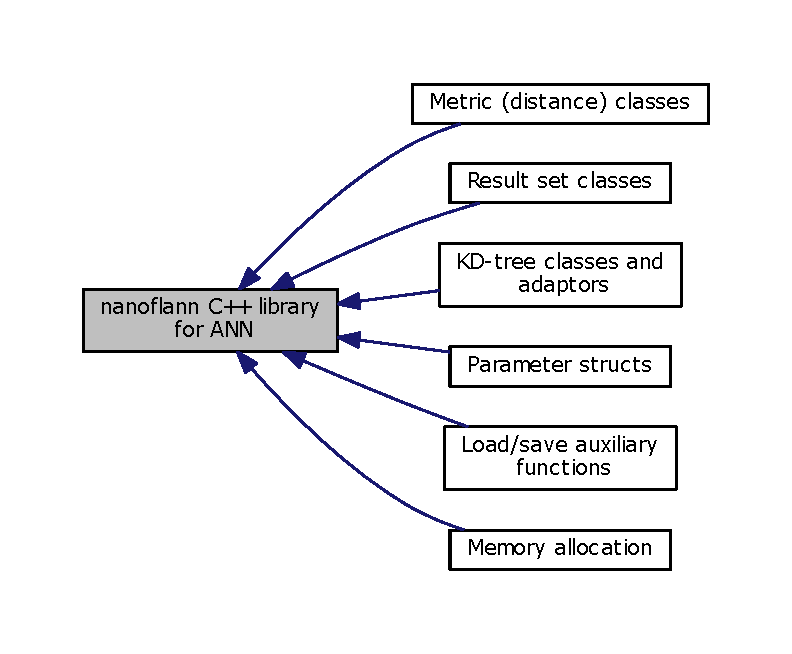
\includegraphics[width=350pt]{group__nanoflann__grp}
\end{center}
\end{figure}
\subsection*{Modules}
\begin{DoxyCompactItemize}
\item 
\hyperlink{group__result__sets__grp}{Result set classes}
\item 
\hyperlink{group__loadsave__grp}{Load/save auxiliary functions}
\item 
\hyperlink{group__metric__grp}{Metric (distance) classes}
\item 
\hyperlink{group__param__grp}{Parameter structs}
\item 
\hyperlink{group__memalloc__grp}{Memory allocation}
\item 
\hyperlink{group__kdtrees__grp}{K\-D-\/tree classes and adaptors}
\end{DoxyCompactItemize}
\subsection*{Macros}
\begin{DoxyCompactItemize}
\item 
\#define \hyperlink{group__nanoflann__grp_ga7b8efca796d8e1861a432a5f6b8404a1}{N\-A\-N\-O\-F\-L\-A\-N\-N\-\_\-\-V\-E\-R\-S\-I\-O\-N}~0x114
\end{DoxyCompactItemize}


\subsection{Detailed Description}


\subsection{Macro Definition Documentation}
\hypertarget{group__nanoflann__grp_ga7b8efca796d8e1861a432a5f6b8404a1}{\index{nanoflann C++ library for A\-N\-N@{nanoflann C++ library for A\-N\-N}!N\-A\-N\-O\-F\-L\-A\-N\-N\-\_\-\-V\-E\-R\-S\-I\-O\-N@{N\-A\-N\-O\-F\-L\-A\-N\-N\-\_\-\-V\-E\-R\-S\-I\-O\-N}}
\index{N\-A\-N\-O\-F\-L\-A\-N\-N\-\_\-\-V\-E\-R\-S\-I\-O\-N@{N\-A\-N\-O\-F\-L\-A\-N\-N\-\_\-\-V\-E\-R\-S\-I\-O\-N}!nanoflann C++ library for ANN@{nanoflann C++ library for A\-N\-N}}
\subsubsection[{N\-A\-N\-O\-F\-L\-A\-N\-N\-\_\-\-V\-E\-R\-S\-I\-O\-N}]{\setlength{\rightskip}{0pt plus 5cm}\#define N\-A\-N\-O\-F\-L\-A\-N\-N\-\_\-\-V\-E\-R\-S\-I\-O\-N~0x114}}\label{group__nanoflann__grp_ga7b8efca796d8e1861a432a5f6b8404a1}
Library version\-: 0x\-Mm\-P (M=Major,m=minor,P=path) 
\hypertarget{group__result__sets__grp}{\section{Result set classes}
\label{group__result__sets__grp}\index{Result set classes@{Result set classes}}
}
Collaboration diagram for Result set classes\-:
\nopagebreak
\begin{figure}[H]
\begin{center}
\leavevmode
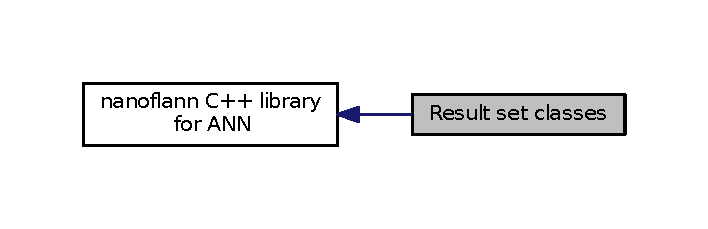
\includegraphics[width=344pt]{group__result__sets__grp}
\end{center}
\end{figure}
\subsection*{Classes}
\begin{DoxyCompactItemize}
\item 
class \hyperlink{classnanoflann_1_1_k_n_n_result_set}{nanoflann\-::\-K\-N\-N\-Result\-Set$<$ Distance\-Type, Index\-Type, Count\-Type $>$}
\item 
class \hyperlink{classnanoflann_1_1_radius_result_set}{nanoflann\-::\-Radius\-Result\-Set$<$ Distance\-Type, Index\-Type $>$}
\item 
struct \hyperlink{structnanoflann_1_1_index_dist___sorter}{nanoflann\-::\-Index\-Dist\-\_\-\-Sorter}
\end{DoxyCompactItemize}


\subsection{Detailed Description}

\hypertarget{group__loadsave__grp}{\section{Load/save auxiliary functions}
\label{group__loadsave__grp}\index{Load/save auxiliary functions@{Load/save auxiliary functions}}
}
Collaboration diagram for Load/save auxiliary functions\-:\nopagebreak
\begin{figure}[H]
\begin{center}
\leavevmode
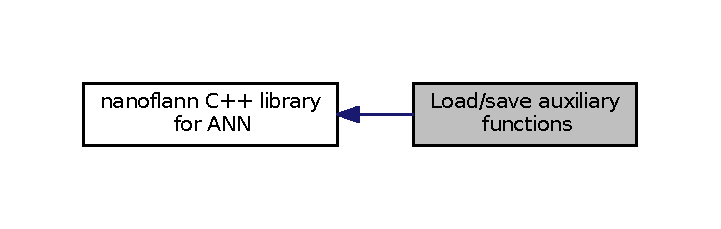
\includegraphics[width=346pt]{group__loadsave__grp}
\end{center}
\end{figure}
\subsection*{Functions}
\begin{DoxyCompactItemize}
\item 
{\footnotesize template$<$typename T $>$ }\\void \hyperlink{group__loadsave__grp_gadf909159ea32f125f71328d00ac2de8d}{nanoflann\-::save\-\_\-value} (F\-I\-L\-E $\ast$stream, const T \&value, size\-\_\-t count=1)
\item 
{\footnotesize template$<$typename T $>$ }\\void \hyperlink{group__loadsave__grp_gac767ee9c25febe0cd6af3ac2e186ffe7}{nanoflann\-::save\-\_\-value} (F\-I\-L\-E $\ast$stream, const std\-::vector$<$ T $>$ \&value)
\item 
{\footnotesize template$<$typename T $>$ }\\void \hyperlink{group__loadsave__grp_ga81940cd63b9ae619251d612d0ddbc819}{nanoflann\-::load\-\_\-value} (F\-I\-L\-E $\ast$stream, T \&value, size\-\_\-t count=1)
\item 
{\footnotesize template$<$typename T $>$ }\\void \hyperlink{group__loadsave__grp_gaefed46e8576d6ce3f1796bb13387ad3d}{nanoflann\-::load\-\_\-value} (F\-I\-L\-E $\ast$stream, std\-::vector$<$ T $>$ \&value)
\end{DoxyCompactItemize}


\subsection{Detailed Description}


\subsection{Function Documentation}
\hypertarget{group__loadsave__grp_ga81940cd63b9ae619251d612d0ddbc819}{\index{Load/save auxiliary functions@{Load/save auxiliary functions}!load\-\_\-value@{load\-\_\-value}}
\index{load\-\_\-value@{load\-\_\-value}!Load/save auxiliary functions@{Load/save auxiliary functions}}
\subsubsection[{load\-\_\-value}]{\setlength{\rightskip}{0pt plus 5cm}template$<$typename T $>$ void nanoflann\-::load\-\_\-value (
\begin{DoxyParamCaption}
\item[{F\-I\-L\-E $\ast$}]{stream, }
\item[{T \&}]{value, }
\item[{size\-\_\-t}]{count = {\ttfamily 1}}
\end{DoxyParamCaption}
)}}\label{group__loadsave__grp_ga81940cd63b9ae619251d612d0ddbc819}
\hypertarget{group__loadsave__grp_gaefed46e8576d6ce3f1796bb13387ad3d}{\index{Load/save auxiliary functions@{Load/save auxiliary functions}!load\-\_\-value@{load\-\_\-value}}
\index{load\-\_\-value@{load\-\_\-value}!Load/save auxiliary functions@{Load/save auxiliary functions}}
\subsubsection[{load\-\_\-value}]{\setlength{\rightskip}{0pt plus 5cm}template$<$typename T $>$ void nanoflann\-::load\-\_\-value (
\begin{DoxyParamCaption}
\item[{F\-I\-L\-E $\ast$}]{stream, }
\item[{std\-::vector$<$ T $>$ \&}]{value}
\end{DoxyParamCaption}
)}}\label{group__loadsave__grp_gaefed46e8576d6ce3f1796bb13387ad3d}


Here is the call graph for this function\-:\nopagebreak
\begin{figure}[H]
\begin{center}
\leavevmode
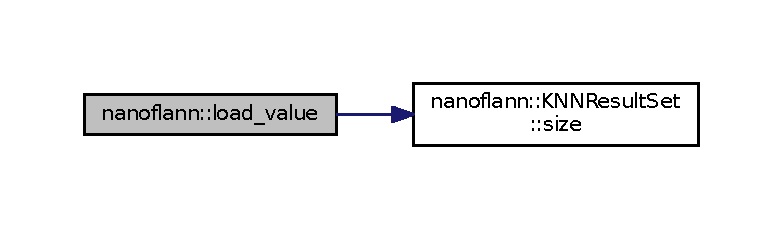
\includegraphics[width=350pt]{group__loadsave__grp_gaefed46e8576d6ce3f1796bb13387ad3d_cgraph}
\end{center}
\end{figure}


\hypertarget{group__loadsave__grp_gadf909159ea32f125f71328d00ac2de8d}{\index{Load/save auxiliary functions@{Load/save auxiliary functions}!save\-\_\-value@{save\-\_\-value}}
\index{save\-\_\-value@{save\-\_\-value}!Load/save auxiliary functions@{Load/save auxiliary functions}}
\subsubsection[{save\-\_\-value}]{\setlength{\rightskip}{0pt plus 5cm}template$<$typename T $>$ void nanoflann\-::save\-\_\-value (
\begin{DoxyParamCaption}
\item[{F\-I\-L\-E $\ast$}]{stream, }
\item[{const T \&}]{value, }
\item[{size\-\_\-t}]{count = {\ttfamily 1}}
\end{DoxyParamCaption}
)}}\label{group__loadsave__grp_gadf909159ea32f125f71328d00ac2de8d}
\hypertarget{group__loadsave__grp_gac767ee9c25febe0cd6af3ac2e186ffe7}{\index{Load/save auxiliary functions@{Load/save auxiliary functions}!save\-\_\-value@{save\-\_\-value}}
\index{save\-\_\-value@{save\-\_\-value}!Load/save auxiliary functions@{Load/save auxiliary functions}}
\subsubsection[{save\-\_\-value}]{\setlength{\rightskip}{0pt plus 5cm}template$<$typename T $>$ void nanoflann\-::save\-\_\-value (
\begin{DoxyParamCaption}
\item[{F\-I\-L\-E $\ast$}]{stream, }
\item[{const std\-::vector$<$ T $>$ \&}]{value}
\end{DoxyParamCaption}
)}}\label{group__loadsave__grp_gac767ee9c25febe0cd6af3ac2e186ffe7}


Here is the call graph for this function\-:\nopagebreak
\begin{figure}[H]
\begin{center}
\leavevmode
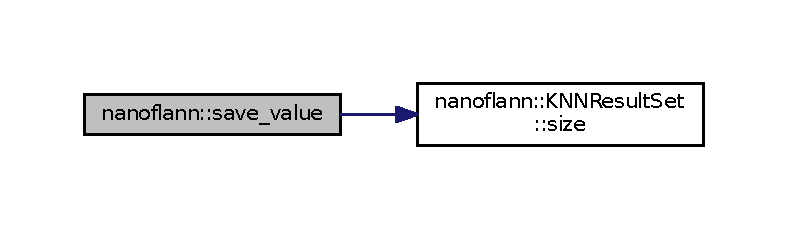
\includegraphics[width=350pt]{group__loadsave__grp_gac767ee9c25febe0cd6af3ac2e186ffe7_cgraph}
\end{center}
\end{figure}



\hypertarget{group__metric__grp}{\section{Metric (distance) classes}
\label{group__metric__grp}\index{Metric (distance) classes@{Metric (distance) classes}}
}
Collaboration diagram for Metric (distance) classes\-:\nopagebreak
\begin{figure}[H]
\begin{center}
\leavevmode
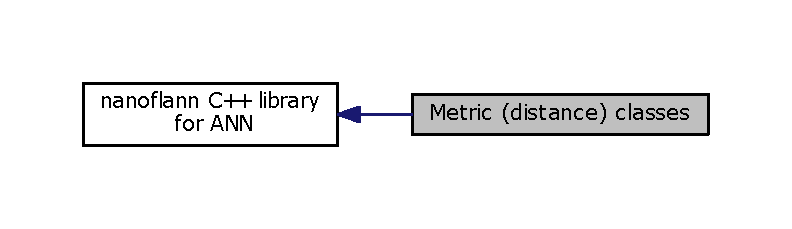
\includegraphics[width=350pt]{group__metric__grp}
\end{center}
\end{figure}
\subsection*{Classes}
\begin{DoxyCompactItemize}
\item 
struct \hyperlink{structnanoflann_1_1_l1___adaptor}{nanoflann\-::\-L1\-\_\-\-Adaptor$<$ T, Data\-Source, \-\_\-\-Distance\-Type $>$}
\item 
struct \hyperlink{structnanoflann_1_1_l2___adaptor}{nanoflann\-::\-L2\-\_\-\-Adaptor$<$ T, Data\-Source, \-\_\-\-Distance\-Type $>$}
\item 
struct \hyperlink{structnanoflann_1_1_l2___simple___adaptor}{nanoflann\-::\-L2\-\_\-\-Simple\-\_\-\-Adaptor$<$ T, Data\-Source, \-\_\-\-Distance\-Type $>$}
\item 
struct \hyperlink{structnanoflann_1_1metric___l1}{nanoflann\-::metric\-\_\-\-L1}
\item 
struct \hyperlink{structnanoflann_1_1metric___l2}{nanoflann\-::metric\-\_\-\-L2}
\item 
struct \hyperlink{structnanoflann_1_1metric___l2___simple}{nanoflann\-::metric\-\_\-\-L2\-\_\-\-Simple}
\end{DoxyCompactItemize}
\subsection*{Functions}
\begin{DoxyCompactItemize}
\item 
{\footnotesize template$<$typename T $>$ }\\T \hyperlink{group__metric__grp_gaf15608f8914516f8d949a8c053d55021}{nanoflann\-::abs} (T x)
\item 
{\footnotesize template$<$$>$ }\\int \hyperlink{group__metric__grp_ga5c50e8d34773da556210ad34d6157763}{nanoflann\-::abs$<$ int $>$} (int x)
\item 
{\footnotesize template$<$$>$ }\\float \hyperlink{group__metric__grp_ga3c252a1b86662381fd025b0576124c2d}{nanoflann\-::abs$<$ float $>$} (float x)
\item 
{\footnotesize template$<$$>$ }\\double \hyperlink{group__metric__grp_ga3fb0513e5af33647f17713a36b10f156}{nanoflann\-::abs$<$ double $>$} (double x)
\item 
{\footnotesize template$<$$>$ }\\long double \hyperlink{group__metric__grp_ga02cfdf1bf211628b049ffd239a26e57e}{nanoflann\-::abs$<$ long double $>$} (long double x)
\end{DoxyCompactItemize}


\subsection{Detailed Description}


\subsection{Function Documentation}
\hypertarget{group__metric__grp_gaf15608f8914516f8d949a8c053d55021}{\index{Metric (distance) classes@{Metric (distance) classes}!abs@{abs}}
\index{abs@{abs}!Metric (distance) classes@{Metric (distance) classes}}
\subsubsection[{abs}]{\setlength{\rightskip}{0pt plus 5cm}template$<$typename T $>$ T nanoflann\-::abs (
\begin{DoxyParamCaption}
\item[{T}]{x}
\end{DoxyParamCaption}
)\hspace{0.3cm}{\ttfamily [inline]}}}\label{group__metric__grp_gaf15608f8914516f8d949a8c053d55021}
\hypertarget{group__metric__grp_ga3fb0513e5af33647f17713a36b10f156}{\index{Metric (distance) classes@{Metric (distance) classes}!abs$<$ double $>$@{abs$<$ double $>$}}
\index{abs$<$ double $>$@{abs$<$ double $>$}!Metric (distance) classes@{Metric (distance) classes}}
\subsubsection[{abs$<$ double $>$}]{\setlength{\rightskip}{0pt plus 5cm}template$<$$>$ double {\bf nanoflann\-::abs}$<$ double $>$ (
\begin{DoxyParamCaption}
\item[{double}]{x}
\end{DoxyParamCaption}
)\hspace{0.3cm}{\ttfamily [inline]}}}\label{group__metric__grp_ga3fb0513e5af33647f17713a36b10f156}
\hypertarget{group__metric__grp_ga3c252a1b86662381fd025b0576124c2d}{\index{Metric (distance) classes@{Metric (distance) classes}!abs$<$ float $>$@{abs$<$ float $>$}}
\index{abs$<$ float $>$@{abs$<$ float $>$}!Metric (distance) classes@{Metric (distance) classes}}
\subsubsection[{abs$<$ float $>$}]{\setlength{\rightskip}{0pt plus 5cm}template$<$$>$ float {\bf nanoflann\-::abs}$<$ float $>$ (
\begin{DoxyParamCaption}
\item[{float}]{x}
\end{DoxyParamCaption}
)\hspace{0.3cm}{\ttfamily [inline]}}}\label{group__metric__grp_ga3c252a1b86662381fd025b0576124c2d}
\hypertarget{group__metric__grp_ga5c50e8d34773da556210ad34d6157763}{\index{Metric (distance) classes@{Metric (distance) classes}!abs$<$ int $>$@{abs$<$ int $>$}}
\index{abs$<$ int $>$@{abs$<$ int $>$}!Metric (distance) classes@{Metric (distance) classes}}
\subsubsection[{abs$<$ int $>$}]{\setlength{\rightskip}{0pt plus 5cm}template$<$$>$ int {\bf nanoflann\-::abs}$<$ int $>$ (
\begin{DoxyParamCaption}
\item[{int}]{x}
\end{DoxyParamCaption}
)\hspace{0.3cm}{\ttfamily [inline]}}}\label{group__metric__grp_ga5c50e8d34773da556210ad34d6157763}


Here is the call graph for this function\-:\nopagebreak
\begin{figure}[H]
\begin{center}
\leavevmode
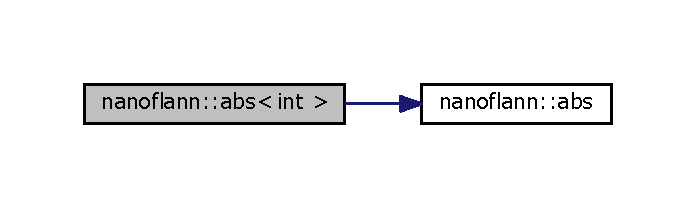
\includegraphics[width=326pt]{group__metric__grp_ga5c50e8d34773da556210ad34d6157763_cgraph}
\end{center}
\end{figure}


\hypertarget{group__metric__grp_ga02cfdf1bf211628b049ffd239a26e57e}{\index{Metric (distance) classes@{Metric (distance) classes}!abs$<$ long double $>$@{abs$<$ long double $>$}}
\index{abs$<$ long double $>$@{abs$<$ long double $>$}!Metric (distance) classes@{Metric (distance) classes}}
\subsubsection[{abs$<$ long double $>$}]{\setlength{\rightskip}{0pt plus 5cm}template$<$$>$ long double {\bf nanoflann\-::abs}$<$ long double $>$ (
\begin{DoxyParamCaption}
\item[{long double}]{x}
\end{DoxyParamCaption}
)\hspace{0.3cm}{\ttfamily [inline]}}}\label{group__metric__grp_ga02cfdf1bf211628b049ffd239a26e57e}

\hypertarget{group__param__grp}{\section{Parameter structs}
\label{group__param__grp}\index{Parameter structs@{Parameter structs}}
}
Collaboration diagram for Parameter structs\-:
\nopagebreak
\begin{figure}[H]
\begin{center}
\leavevmode
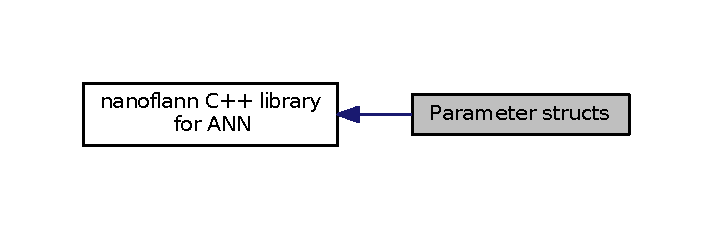
\includegraphics[width=344pt]{group__param__grp}
\end{center}
\end{figure}
\subsection*{Classes}
\begin{DoxyCompactItemize}
\item 
struct \hyperlink{structnanoflann_1_1_k_d_tree_single_index_adaptor_params}{nanoflann\-::\-K\-D\-Tree\-Single\-Index\-Adaptor\-Params}
\item 
struct \hyperlink{structnanoflann_1_1_search_params}{nanoflann\-::\-Search\-Params}
\end{DoxyCompactItemize}


\subsection{Detailed Description}

\hypertarget{group__memalloc__grp}{\section{Memory allocation}
\label{group__memalloc__grp}\index{Memory allocation@{Memory allocation}}
}
Collaboration diagram for Memory allocation\-:
\nopagebreak
\begin{figure}[H]
\begin{center}
\leavevmode
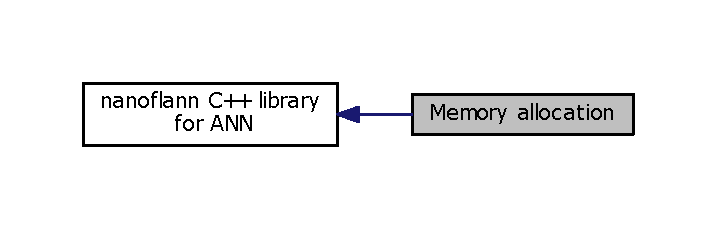
\includegraphics[width=344pt]{group__memalloc__grp}
\end{center}
\end{figure}
\subsection*{Classes}
\begin{DoxyCompactItemize}
\item 
class \hyperlink{classnanoflann_1_1_pooled_allocator}{nanoflann\-::\-Pooled\-Allocator}
\end{DoxyCompactItemize}
\subsection*{Functions}
\begin{DoxyCompactItemize}
\item 
{\footnotesize template$<$typename T $>$ }\\T $\ast$ \hyperlink{group__memalloc__grp_ga477667da2a8edb1d65f5a7eebaffc1eb}{nanoflann\-::allocate} (size\-\_\-t count=1)
\end{DoxyCompactItemize}
\subsection*{Variables}
\begin{DoxyCompactItemize}
\item 
const size\-\_\-t \hyperlink{group__memalloc__grp_ga40956ef8f797399b4f478df9fc1566f4}{nanoflann\-::\-W\-O\-R\-D\-S\-I\-Z\-E} =16
\item 
const size\-\_\-t \hyperlink{group__memalloc__grp_gaf4df087b6f47e514f6062f7ada2d19d7}{nanoflann\-::\-B\-L\-O\-C\-K\-S\-I\-Z\-E} =8192
\end{DoxyCompactItemize}


\subsection{Detailed Description}


\subsection{Function Documentation}
\hypertarget{group__memalloc__grp_ga477667da2a8edb1d65f5a7eebaffc1eb}{\index{Memory allocation@{Memory allocation}!allocate@{allocate}}
\index{allocate@{allocate}!Memory allocation@{Memory allocation}}
\subsubsection[{allocate}]{\setlength{\rightskip}{0pt plus 5cm}template$<$typename T $>$ T$\ast$ nanoflann\-::allocate (
\begin{DoxyParamCaption}
\item[{size\-\_\-t}]{count = {\ttfamily 1}}
\end{DoxyParamCaption}
)\hspace{0.3cm}{\ttfamily [inline]}}}\label{group__memalloc__grp_ga477667da2a8edb1d65f5a7eebaffc1eb}
Allocates (using C's malloc) a generic type T.

Params\-: count = number of instances to allocate. Returns\-: pointer (of type T$\ast$) to memory buffer 

\subsection{Variable Documentation}
\hypertarget{group__memalloc__grp_gaf4df087b6f47e514f6062f7ada2d19d7}{\index{Memory allocation@{Memory allocation}!B\-L\-O\-C\-K\-S\-I\-Z\-E@{B\-L\-O\-C\-K\-S\-I\-Z\-E}}
\index{B\-L\-O\-C\-K\-S\-I\-Z\-E@{B\-L\-O\-C\-K\-S\-I\-Z\-E}!Memory allocation@{Memory allocation}}
\subsubsection[{B\-L\-O\-C\-K\-S\-I\-Z\-E}]{\setlength{\rightskip}{0pt plus 5cm}const size\-\_\-t nanoflann\-::\-B\-L\-O\-C\-K\-S\-I\-Z\-E =8192}}\label{group__memalloc__grp_gaf4df087b6f47e514f6062f7ada2d19d7}
\hypertarget{group__memalloc__grp_ga40956ef8f797399b4f478df9fc1566f4}{\index{Memory allocation@{Memory allocation}!W\-O\-R\-D\-S\-I\-Z\-E@{W\-O\-R\-D\-S\-I\-Z\-E}}
\index{W\-O\-R\-D\-S\-I\-Z\-E@{W\-O\-R\-D\-S\-I\-Z\-E}!Memory allocation@{Memory allocation}}
\subsubsection[{W\-O\-R\-D\-S\-I\-Z\-E}]{\setlength{\rightskip}{0pt plus 5cm}const size\-\_\-t nanoflann\-::\-W\-O\-R\-D\-S\-I\-Z\-E =16}}\label{group__memalloc__grp_ga40956ef8f797399b4f478df9fc1566f4}
Pooled storage allocator

The following routines allow for the efficient allocation of storage in small chunks from a specified pool. Rather than allowing each structure to be freed individually, an entire pool of storage is freed at once. This method has two advantages over just using malloc() and free(). First, it is far more efficient for allocating small objects, as there is no overhead for remembering all the information needed to free each object or consolidating fragmented memory. Second, the decision about how long to keep an object is made at the time of allocation, and there is no need to track down all the objects to free them. 
\hypertarget{group__kdtrees__grp}{\section{K\-D-\/tree classes and adaptors}
\label{group__kdtrees__grp}\index{K\-D-\/tree classes and adaptors@{K\-D-\/tree classes and adaptors}}
}
Collaboration diagram for K\-D-\/tree classes and adaptors\-:\nopagebreak
\begin{figure}[H]
\begin{center}
\leavevmode
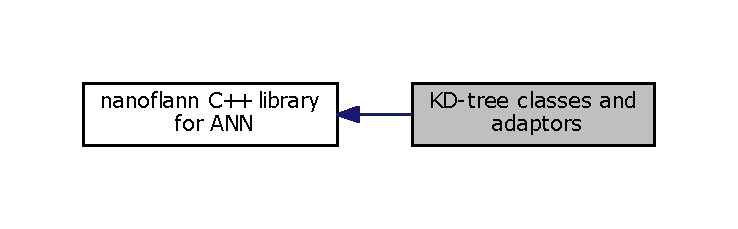
\includegraphics[width=350pt]{group__kdtrees__grp}
\end{center}
\end{figure}
\subsection*{Classes}
\begin{DoxyCompactItemize}
\item 
class \hyperlink{classnanoflann_1_1_k_d_tree_single_index_adaptor}{nanoflann\-::\-K\-D\-Tree\-Single\-Index\-Adaptor$<$ Distance, Dataset\-Adaptor, D\-I\-M, Index\-Type $>$}
\item 
struct \hyperlink{structnanoflann_1_1_k_d_tree_eigen_matrix_adaptor}{nanoflann\-::\-K\-D\-Tree\-Eigen\-Matrix\-Adaptor$<$ Matrix\-Type, D\-I\-M, Distance, Index\-Type $>$}
\end{DoxyCompactItemize}


\subsection{Detailed Description}

\chapter{Namespace Documentation}
\hypertarget{namespaceboost}{\section{boost Namespace Reference}
\label{namespaceboost}\index{boost@{boost}}
}

\hypertarget{namespaceccmc}{\section{ccmc Namespace Reference}
\label{namespaceccmc}\index{ccmc@{ccmc}}
}


Namespace for the Community Coordinated Modeling Center code.  


\subsection*{Namespaces}
\begin{DoxyCompactItemize}
\item 
\hyperlink{namespaceccmc_1_1constants}{constants}
\item 
\hyperlink{namespaceccmc_1_1defaults}{defaults}
\item 
\hyperlink{namespaceccmc_1_1strings}{strings}
\end{DoxyCompactItemize}
\subsection*{Classes}
\begin{DoxyCompactItemize}
\item 
struct \hyperlink{structccmc_1_1_smart_grid_search_values}{Smart\-Grid\-Search\-Values}
\item 
class \hyperlink{classccmc_1_1_adapt3_d}{Adapt3\-D}
\begin{DoxyCompactList}\small\item\em T\-O\-D\-O\-: brief description of \hyperlink{classccmc_1_1_adapt3_d}{Adapt3\-D} class. \end{DoxyCompactList}\item 
class \hyperlink{classccmc_1_1_adapt3_d_interpolator}{Adapt3\-D\-Interpolator}
\begin{DoxyCompactList}\small\item\em T\-O\-D\-O\-: brief description of \hyperlink{classccmc_1_1_b_a_t_s_r_u_s_interpolator}{B\-A\-T\-S\-R\-U\-S\-Interpolator} class. \end{DoxyCompactList}\item 
class \hyperlink{classccmc_1_1_attribute}{Attribute}
\begin{DoxyCompactList}\small\item\em T\-O\-D\-O\-: brief description of \hyperlink{classccmc_1_1_attribute}{Attribute} class. \end{DoxyCompactList}\item 
class \hyperlink{classccmc_1_1_b_a_t_s_r_u_s}{B\-A\-T\-S\-R\-U\-S}
\begin{DoxyCompactList}\small\item\em T\-O\-D\-O\-: brief description of \hyperlink{classccmc_1_1_b_a_t_s_r_u_s}{B\-A\-T\-S\-R\-U\-S} class. \end{DoxyCompactList}\item 
class \hyperlink{classccmc_1_1_b_a_t_s_r_u_s_interpolator}{B\-A\-T\-S\-R\-U\-S\-Interpolator}
\begin{DoxyCompactList}\small\item\em T\-O\-D\-O\-: brief description of \hyperlink{classccmc_1_1_b_a_t_s_r_u_s_interpolator}{B\-A\-T\-S\-R\-U\-S\-Interpolator} class. \end{DoxyCompactList}\item 
class \hyperlink{classccmc_1_1_time}{Time}
\item 
class \hyperlink{classccmc_1_1_c_d_f_file_reader}{C\-D\-F\-File\-Reader}
\item 
class \hyperlink{classccmc_1_1_c_t_i_p}{C\-T\-I\-P}
\begin{DoxyCompactList}\small\item\em T\-O\-D\-O\-: Brief description of \hyperlink{classccmc_1_1_c_t_i_p}{C\-T\-I\-P} class. \end{DoxyCompactList}\item 
class \hyperlink{classccmc_1_1_e_n_l_i_l}{E\-N\-L\-I\-L}
\begin{DoxyCompactList}\small\item\em T\-O\-D\-O\-: Brief description of \hyperlink{classccmc_1_1_e_n_l_i_l}{E\-N\-L\-I\-L} class. \end{DoxyCompactList}\item 
class \hyperlink{classccmc_1_1_e_n_l_i_l_interpolator}{E\-N\-L\-I\-L\-Interpolator}
\begin{DoxyCompactList}\small\item\em T\-O\-D\-O\-: Brief description of \hyperlink{classccmc_1_1_e_n_l_i_l_interpolator}{E\-N\-L\-I\-L\-Interpolator} class. \end{DoxyCompactList}\item 
class \hyperlink{classccmc_1_1_fieldline}{Fieldline}
\item 
class \hyperlink{classccmc_1_1_file_reader}{File\-Reader}
\begin{DoxyCompactList}\small\item\em T\-O\-D\-O\-: Brief description of \hyperlink{classccmc_1_1_file_reader}{File\-Reader} class. \end{DoxyCompactList}\item 
class \hyperlink{classccmc_1_1_general_file_reader}{General\-File\-Reader}
\item 
class \hyperlink{classccmc_1_1_interpolator}{Interpolator}
\begin{DoxyCompactList}\small\item\em T\-O\-D\-O\-: Brief description of \hyperlink{classccmc_1_1_interpolator}{Interpolator} class. \end{DoxyCompactList}\item 
class \hyperlink{classccmc_1_1_kameleon_interpolator}{Kameleon\-Interpolator}
\begin{DoxyCompactList}\small\item\em T\-O\-D\-O\-: Brief description of \hyperlink{classccmc_1_1_kameleon_interpolator}{Kameleon\-Interpolator} class. \end{DoxyCompactList}\item 
class \hyperlink{classccmc_1_1_l_f_m}{L\-F\-M}
\begin{DoxyCompactList}\small\item\em T\-O\-D\-O\-: Brief description of \hyperlink{classccmc_1_1_l_f_m}{L\-F\-M} class. \end{DoxyCompactList}\item 
class \hyperlink{classccmc_1_1_l_f_m_interpolator}{L\-F\-M\-Interpolator}
\begin{DoxyCompactList}\small\item\em T\-O\-D\-O\-: Brief description of \hyperlink{classccmc_1_1_l_f_m_interpolator}{L\-F\-M\-Interpolator} class. \end{DoxyCompactList}\item 
class \hyperlink{classccmc_1_1_grid_polyhedron}{Grid\-Polyhedron}
\item 
class \hyperlink{classccmc_1_1_axis_polyhedron}{Axis\-Polyhedron}
\item 
class \hyperlink{classccmc_1_1_j_poly}{J\-Poly}
\item 
class \hyperlink{classccmc_1_1_i_poly}{I\-Poly}
\item 
class \hyperlink{classccmc_1_1_magnetogram}{Magnetogram}
\begin{DoxyCompactList}\small\item\em T\-O\-D\-O\-: Brief description of \hyperlink{classccmc_1_1_magnetogram}{Magnetogram} class. \end{DoxyCompactList}\item 
class \hyperlink{classccmc_1_1_magnetogram_interpolator}{Magnetogram\-Interpolator}
\begin{DoxyCompactList}\small\item\em T\-O\-D\-O\-: Brief description of \hyperlink{classccmc_1_1_magnetogram_interpolator}{Magnetogram\-Interpolator} class. \end{DoxyCompactList}\item 
class \hyperlink{classccmc_1_1_m_a_s}{M\-A\-S}
\begin{DoxyCompactList}\small\item\em T\-O\-D\-O\-: Brief description of \hyperlink{classccmc_1_1_m_a_s}{M\-A\-S} class. \end{DoxyCompactList}\item 
class \hyperlink{classccmc_1_1_m_a_s_interpolator}{M\-A\-S\-Interpolator}
\begin{DoxyCompactList}\small\item\em T\-O\-D\-O\-: Brief description of \hyperlink{classccmc_1_1_m_a_s_interpolator}{M\-A\-S\-Interpolator} class. \end{DoxyCompactList}\item 
class \hyperlink{classccmc_1_1_math}{Math}
\item 
class \hyperlink{classccmc_1_1_model}{Model}
\begin{DoxyCompactList}\small\item\em T\-O\-D\-O\-: Brief description of \hyperlink{classccmc_1_1_model}{Model} class. \end{DoxyCompactList}\item 
class \hyperlink{classccmc_1_1_open_g_g_c_m}{Open\-G\-G\-C\-M}
\begin{DoxyCompactList}\small\item\em T\-O\-D\-O\-: Brief description of \hyperlink{classccmc_1_1_open_g_g_c_m}{Open\-G\-G\-C\-M} class. \end{DoxyCompactList}\item 
class \hyperlink{classccmc_1_1_open_g_g_c_m_interpolator}{Open\-G\-G\-C\-M\-Interpolator}
\begin{DoxyCompactList}\small\item\em T\-O\-D\-O\-: Brief description of \hyperlink{classccmc_1_1_open_g_g_c_m_interpolator}{Open\-G\-G\-C\-M\-Interpolator} class. \end{DoxyCompactList}\item 
class \hyperlink{classccmc_1_1_point}{Point}
\begin{DoxyCompactList}\small\item\em T\-O\-D\-O\-: Brief description of \hyperlink{classccmc_1_1_point}{Point} class. \end{DoxyCompactList}\item 
class \hyperlink{classccmc_1_1_point3f}{Point3f}
\item 
class \hyperlink{classccmc_1_1_polyhedron}{Polyhedron}
\item 
class \hyperlink{classccmc_1_1_s_w_m_f_iono}{S\-W\-M\-F\-Iono}
\item 
class \hyperlink{classccmc_1_1_s_w_m_f_iono_interpolator}{S\-W\-M\-F\-Iono\-Interpolator}
\item 
class \hyperlink{classccmc_1_1_time_interpolator}{Time\-Interpolator}
\item 
class \hyperlink{classccmc_1_1_tracer}{Tracer}
\begin{DoxyCompactList}\small\item\em T\-O\-D\-O\-: Brief description. \end{DoxyCompactList}\item 
class \hyperlink{classccmc_1_1_utils}{Utils}
\item 
class \hyperlink{classccmc_1_1_vector}{Vector}
\end{DoxyCompactItemize}
\subsection*{Functions}
\begin{DoxyCompactItemize}
\item 
std\-::ostream \& \hyperlink{namespaceccmc_ad811f4e9ac8644fea4054b81aabbb072}{operator$<$$<$} (std\-::ostream \&out, const \hyperlink{classccmc_1_1_attribute}{Attribute} attribute)
\item 
std\-::ostream \& \hyperlink{namespaceccmc_ae583b649601da0108ffe024b315cc131}{operator$<$$<$} (std\-::ostream \&out, const \hyperlink{classccmc_1_1_time}{Time} time)
\item 
double \hyperlink{namespaceccmc_a56b029527268b2a7dc0152296e790311}{operator-\/} (const \hyperlink{classccmc_1_1_time}{Time} \&time1, const \hyperlink{classccmc_1_1_time}{Time} \&time2)
\item 
bool \hyperlink{namespaceccmc_a3fce93a0ef72e32c4565e23abdb5e19b}{operator==} (const \hyperlink{classccmc_1_1_time}{Time} \&time1, const \hyperlink{classccmc_1_1_time}{Time} \&time2)
\item 
bool \hyperlink{namespaceccmc_ab38851472be407f010420ed9af48f30b}{operator$<$} (const \hyperlink{classccmc_1_1_time}{Time} \&time1, const \hyperlink{classccmc_1_1_time}{Time} \&time2)
\item 
bool \hyperlink{namespaceccmc_aa8187280256650785ed2835b7ee12574}{operator$>$} (const \hyperlink{classccmc_1_1_time}{Time} \&time1, const \hyperlink{classccmc_1_1_time}{Time} \&time2)
\item 
bool \hyperlink{namespaceccmc_a9d79baffce54b78a54946d6a76743c0b}{operator$>$=} (const \hyperlink{classccmc_1_1_time}{Time} \&time1, const \hyperlink{classccmc_1_1_time}{Time} \&time2)
\item 
int \hyperlink{namespaceccmc_a89959a8566a58d1e6c000d742304be1b}{cxform} (const char $\ast$from, const char $\ast$to, const double et, double $\ast$v\-\_\-in, double $\ast$v\-\_\-out)
\item 
double \hyperlink{namespaceccmc_ae9b36fc97f95279e8815455b796fb78f}{gregorian\-\_\-calendar\-\_\-to\-\_\-jd} (int y, int m, int d, int h, int mi, int s)
\item 
long \hyperlink{namespaceccmc_a2bcda52133fe790c98ff1e09e0d8feef}{date2es} (int yyyy, int mm, int dd, int hh, int mm2, int ss)
\item 
long \hyperlink{namespaceccmc_acbeec2fb0bdcdbe669f213d20cb5d3ac}{cx\-Round} (double doub)
\item 
std\-::ostream \& \hyperlink{namespaceccmc_a447a43508de96a63d12aae7c85aaa06b}{operator$<$$<$} (std\-::ostream \&out, const \hyperlink{classccmc_1_1_point3f}{Point3f} \&point)
\item 
std\-::size\-\_\-t \hyperlink{namespaceccmc_a12a62484d27726b55814a116018d6434}{hash\-\_\-value} (\hyperlink{classccmc_1_1_time}{Time} const \&time)
\end{DoxyCompactItemize}


\subsection{Detailed Description}
Namespace for the Community Coordinated Modeling Center code. Full documentation for the ccmc namespace 

\subsection{Function Documentation}
\hypertarget{namespaceccmc_a89959a8566a58d1e6c000d742304be1b}{\index{ccmc@{ccmc}!cxform@{cxform}}
\index{cxform@{cxform}!ccmc@{ccmc}}
\subsubsection[{cxform}]{\setlength{\rightskip}{0pt plus 5cm}int ccmc\-::cxform (
\begin{DoxyParamCaption}
\item[{const char $\ast$}]{from, }
\item[{const char $\ast$}]{to, }
\item[{const double}]{et, }
\item[{double $\ast$}]{v\-\_\-in, }
\item[{double $\ast$}]{v\-\_\-out}
\end{DoxyParamCaption}
)}}\label{namespaceccmc_a89959a8566a58d1e6c000d742304be1b}
\hypertarget{namespaceccmc_acbeec2fb0bdcdbe669f213d20cb5d3ac}{\index{ccmc@{ccmc}!cx\-Round@{cx\-Round}}
\index{cx\-Round@{cx\-Round}!ccmc@{ccmc}}
\subsubsection[{cx\-Round}]{\setlength{\rightskip}{0pt plus 5cm}long ccmc\-::cx\-Round (
\begin{DoxyParamCaption}
\item[{double}]{doub}
\end{DoxyParamCaption}
)}}\label{namespaceccmc_acbeec2fb0bdcdbe669f213d20cb5d3ac}
\hypertarget{namespaceccmc_a2bcda52133fe790c98ff1e09e0d8feef}{\index{ccmc@{ccmc}!date2es@{date2es}}
\index{date2es@{date2es}!ccmc@{ccmc}}
\subsubsection[{date2es}]{\setlength{\rightskip}{0pt plus 5cm}long ccmc\-::date2es (
\begin{DoxyParamCaption}
\item[{int}]{yyyy, }
\item[{int}]{mm, }
\item[{int}]{dd, }
\item[{int}]{hh, }
\item[{int}]{mm2, }
\item[{int}]{ss}
\end{DoxyParamCaption}
)}}\label{namespaceccmc_a2bcda52133fe790c98ff1e09e0d8feef}


Here is the call graph for this function\-:
\nopagebreak
\begin{figure}[H]
\begin{center}
\leavevmode
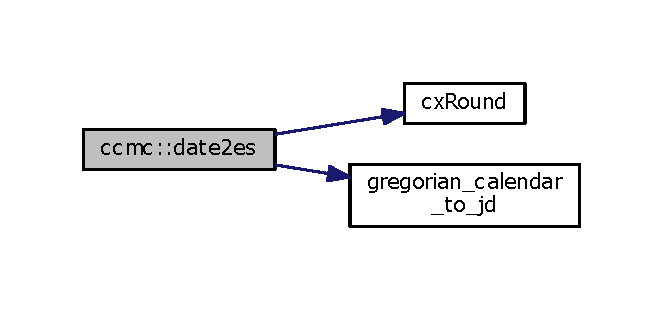
\includegraphics[width=318pt]{namespaceccmc_a2bcda52133fe790c98ff1e09e0d8feef_cgraph}
\end{center}
\end{figure}


\hypertarget{namespaceccmc_ae9b36fc97f95279e8815455b796fb78f}{\index{ccmc@{ccmc}!gregorian\-\_\-calendar\-\_\-to\-\_\-jd@{gregorian\-\_\-calendar\-\_\-to\-\_\-jd}}
\index{gregorian\-\_\-calendar\-\_\-to\-\_\-jd@{gregorian\-\_\-calendar\-\_\-to\-\_\-jd}!ccmc@{ccmc}}
\subsubsection[{gregorian\-\_\-calendar\-\_\-to\-\_\-jd}]{\setlength{\rightskip}{0pt plus 5cm}double ccmc\-::gregorian\-\_\-calendar\-\_\-to\-\_\-jd (
\begin{DoxyParamCaption}
\item[{int}]{y, }
\item[{int}]{m, }
\item[{int}]{d, }
\item[{int}]{h, }
\item[{int}]{mi, }
\item[{int}]{s}
\end{DoxyParamCaption}
)}}\label{namespaceccmc_ae9b36fc97f95279e8815455b796fb78f}
\hypertarget{namespaceccmc_a12a62484d27726b55814a116018d6434}{\index{ccmc@{ccmc}!hash\-\_\-value@{hash\-\_\-value}}
\index{hash\-\_\-value@{hash\-\_\-value}!ccmc@{ccmc}}
\subsubsection[{hash\-\_\-value}]{\setlength{\rightskip}{0pt plus 5cm}std\-::size\-\_\-t ccmc\-::hash\-\_\-value (
\begin{DoxyParamCaption}
\item[{{\bf Time} const \&}]{time}
\end{DoxyParamCaption}
)\hspace{0.3cm}{\ttfamily [inline]}}}\label{namespaceccmc_a12a62484d27726b55814a116018d6434}


Here is the call graph for this function\-:
\nopagebreak
\begin{figure}[H]
\begin{center}
\leavevmode
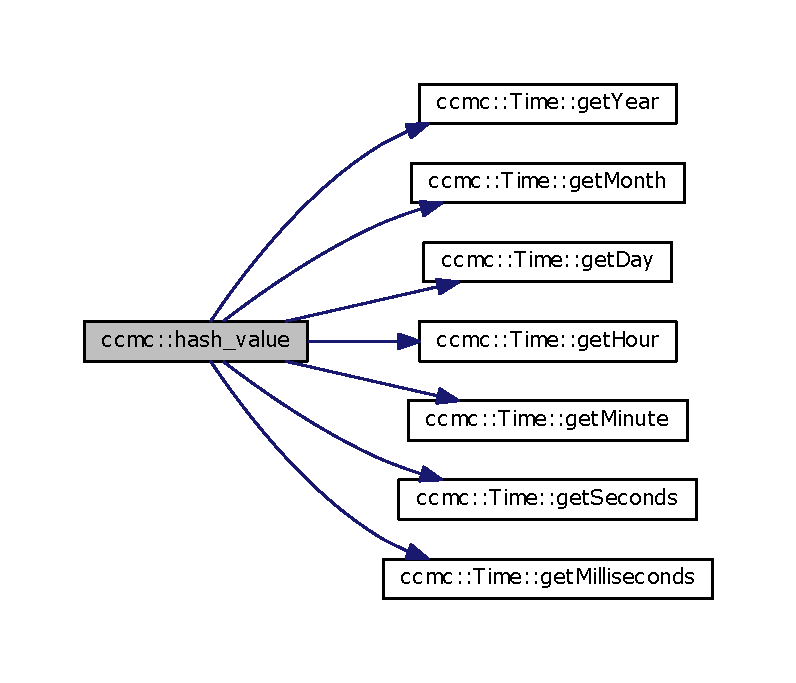
\includegraphics[width=350pt]{namespaceccmc_a12a62484d27726b55814a116018d6434_cgraph}
\end{center}
\end{figure}


\hypertarget{namespaceccmc_a56b029527268b2a7dc0152296e790311}{\index{ccmc@{ccmc}!operator-\/@{operator-\/}}
\index{operator-\/@{operator-\/}!ccmc@{ccmc}}
\subsubsection[{operator-\/}]{\setlength{\rightskip}{0pt plus 5cm}double ccmc\-::operator-\/ (
\begin{DoxyParamCaption}
\item[{const Time \&}]{time1, }
\item[{const Time \&}]{time2}
\end{DoxyParamCaption}
)}}\label{namespaceccmc_a56b029527268b2a7dc0152296e790311}


Here is the call graph for this function\-:
\nopagebreak
\begin{figure}[H]
\begin{center}
\leavevmode
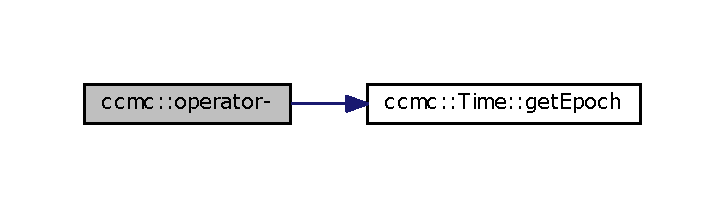
\includegraphics[width=348pt]{namespaceccmc_a56b029527268b2a7dc0152296e790311_cgraph}
\end{center}
\end{figure}


\hypertarget{namespaceccmc_ab38851472be407f010420ed9af48f30b}{\index{ccmc@{ccmc}!operator$<$@{operator$<$}}
\index{operator$<$@{operator$<$}!ccmc@{ccmc}}
\subsubsection[{operator$<$}]{\setlength{\rightskip}{0pt plus 5cm}bool ccmc\-::operator$<$ (
\begin{DoxyParamCaption}
\item[{const Time \&}]{time1, }
\item[{const Time \&}]{time2}
\end{DoxyParamCaption}
)}}\label{namespaceccmc_ab38851472be407f010420ed9af48f30b}


Here is the call graph for this function\-:
\nopagebreak
\begin{figure}[H]
\begin{center}
\leavevmode
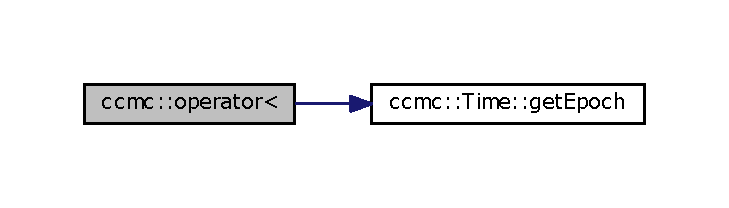
\includegraphics[width=350pt]{namespaceccmc_ab38851472be407f010420ed9af48f30b_cgraph}
\end{center}
\end{figure}


\hypertarget{namespaceccmc_a447a43508de96a63d12aae7c85aaa06b}{\index{ccmc@{ccmc}!operator$<$$<$@{operator$<$$<$}}
\index{operator$<$$<$@{operator$<$$<$}!ccmc@{ccmc}}
\subsubsection[{operator$<$$<$}]{\setlength{\rightskip}{0pt plus 5cm}std\-::ostream\& ccmc\-::operator$<$$<$ (
\begin{DoxyParamCaption}
\item[{std\-::ostream \&}]{out, }
\item[{const Point3f \&}]{point}
\end{DoxyParamCaption}
)}}\label{namespaceccmc_a447a43508de96a63d12aae7c85aaa06b}

\begin{DoxyParams}{Parameters}
{\em out} & \\
\hline
{\em point} & \\
\hline
\end{DoxyParams}
\begin{DoxyReturn}{Returns}

\end{DoxyReturn}


Here is the call graph for this function\-:
\nopagebreak
\begin{figure}[H]
\begin{center}
\leavevmode
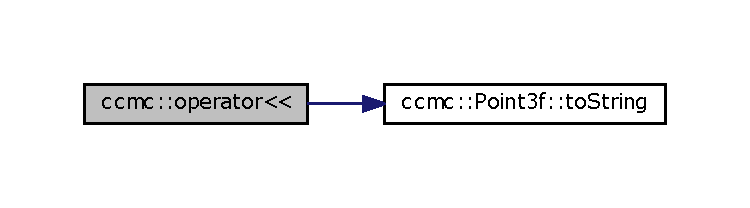
\includegraphics[width=350pt]{namespaceccmc_a447a43508de96a63d12aae7c85aaa06b_cgraph}
\end{center}
\end{figure}


\hypertarget{namespaceccmc_ae583b649601da0108ffe024b315cc131}{\index{ccmc@{ccmc}!operator$<$$<$@{operator$<$$<$}}
\index{operator$<$$<$@{operator$<$$<$}!ccmc@{ccmc}}
\subsubsection[{operator$<$$<$}]{\setlength{\rightskip}{0pt plus 5cm}std\-::ostream \& ccmc\-::operator$<$$<$ (
\begin{DoxyParamCaption}
\item[{std\-::ostream \&}]{out, }
\item[{const Time}]{time}
\end{DoxyParamCaption}
)}}\label{namespaceccmc_ae583b649601da0108ffe024b315cc131}


Here is the call graph for this function\-:
\nopagebreak
\begin{figure}[H]
\begin{center}
\leavevmode
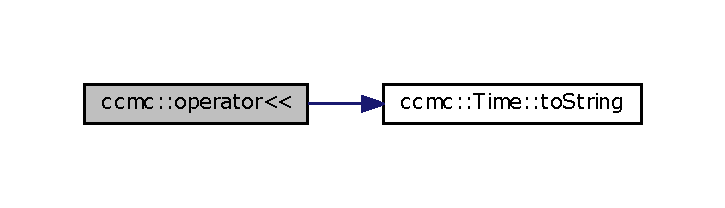
\includegraphics[width=348pt]{namespaceccmc_ae583b649601da0108ffe024b315cc131_cgraph}
\end{center}
\end{figure}


\hypertarget{namespaceccmc_ad811f4e9ac8644fea4054b81aabbb072}{\index{ccmc@{ccmc}!operator$<$$<$@{operator$<$$<$}}
\index{operator$<$$<$@{operator$<$$<$}!ccmc@{ccmc}}
\subsubsection[{operator$<$$<$}]{\setlength{\rightskip}{0pt plus 5cm}std\-::ostream\& ccmc\-::operator$<$$<$ (
\begin{DoxyParamCaption}
\item[{std\-::ostream \&}]{out, }
\item[{const Attribute}]{attribute}
\end{DoxyParamCaption}
)}}\label{namespaceccmc_ad811f4e9ac8644fea4054b81aabbb072}


Here is the call graph for this function\-:
\nopagebreak
\begin{figure}[H]
\begin{center}
\leavevmode
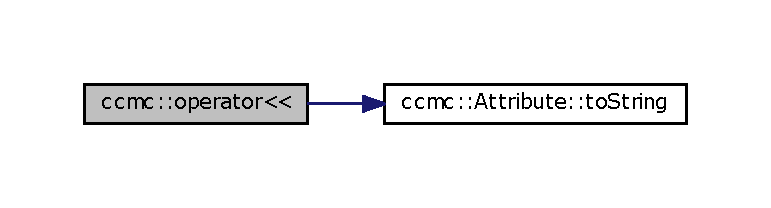
\includegraphics[width=350pt]{namespaceccmc_ad811f4e9ac8644fea4054b81aabbb072_cgraph}
\end{center}
\end{figure}


\hypertarget{namespaceccmc_a3fce93a0ef72e32c4565e23abdb5e19b}{\index{ccmc@{ccmc}!operator==@{operator==}}
\index{operator==@{operator==}!ccmc@{ccmc}}
\subsubsection[{operator==}]{\setlength{\rightskip}{0pt plus 5cm}bool ccmc\-::operator== (
\begin{DoxyParamCaption}
\item[{const Time \&}]{time1, }
\item[{const Time \&}]{time2}
\end{DoxyParamCaption}
)}}\label{namespaceccmc_a3fce93a0ef72e32c4565e23abdb5e19b}


Here is the call graph for this function\-:
\nopagebreak
\begin{figure}[H]
\begin{center}
\leavevmode
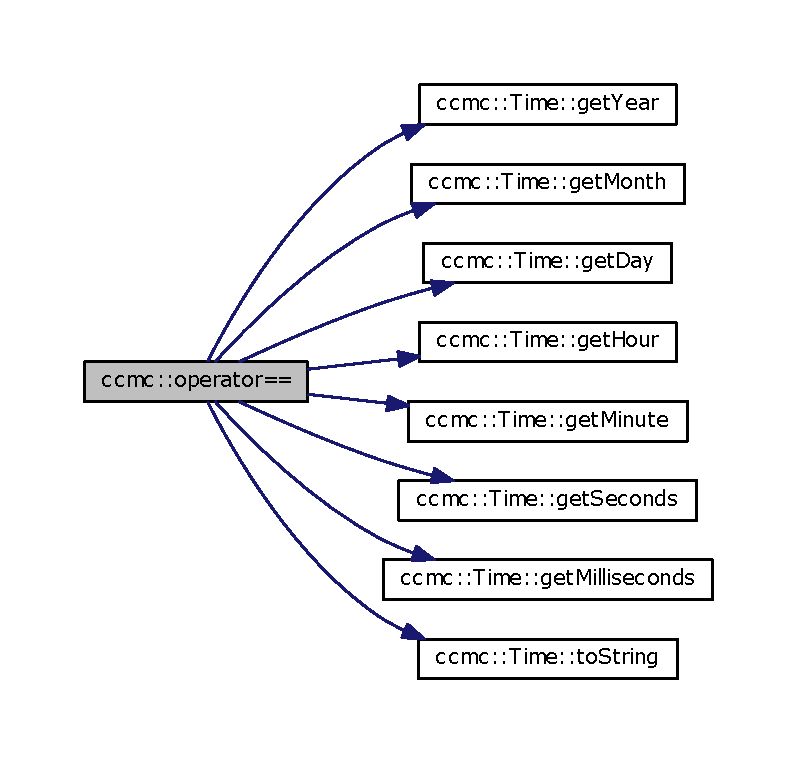
\includegraphics[width=350pt]{namespaceccmc_a3fce93a0ef72e32c4565e23abdb5e19b_cgraph}
\end{center}
\end{figure}


\hypertarget{namespaceccmc_aa8187280256650785ed2835b7ee12574}{\index{ccmc@{ccmc}!operator$>$@{operator$>$}}
\index{operator$>$@{operator$>$}!ccmc@{ccmc}}
\subsubsection[{operator$>$}]{\setlength{\rightskip}{0pt plus 5cm}bool ccmc\-::operator$>$ (
\begin{DoxyParamCaption}
\item[{const Time \&}]{time1, }
\item[{const Time \&}]{time2}
\end{DoxyParamCaption}
)}}\label{namespaceccmc_aa8187280256650785ed2835b7ee12574}


Here is the call graph for this function\-:
\nopagebreak
\begin{figure}[H]
\begin{center}
\leavevmode
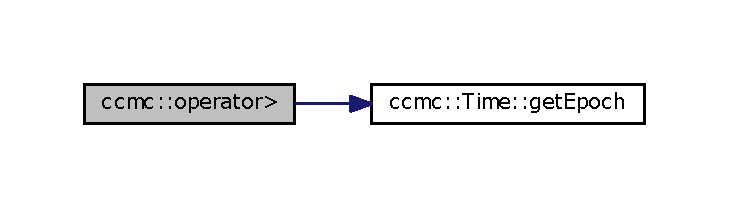
\includegraphics[width=350pt]{namespaceccmc_aa8187280256650785ed2835b7ee12574_cgraph}
\end{center}
\end{figure}


\hypertarget{namespaceccmc_a9d79baffce54b78a54946d6a76743c0b}{\index{ccmc@{ccmc}!operator$>$=@{operator$>$=}}
\index{operator$>$=@{operator$>$=}!ccmc@{ccmc}}
\subsubsection[{operator$>$=}]{\setlength{\rightskip}{0pt plus 5cm}bool ccmc\-::operator$>$= (
\begin{DoxyParamCaption}
\item[{const Time \&}]{time1, }
\item[{const Time \&}]{time2}
\end{DoxyParamCaption}
)}}\label{namespaceccmc_a9d79baffce54b78a54946d6a76743c0b}

\hypertarget{namespaceccmc_1_1constants}{\section{ccmc\-:\-:constants Namespace Reference}
\label{namespaceccmc_1_1constants}\index{ccmc\-::constants@{ccmc\-::constants}}
}

\hypertarget{namespaceccmc_1_1defaults}{\section{ccmc\-:\-:defaults Namespace Reference}
\label{namespaceccmc_1_1defaults}\index{ccmc\-::defaults@{ccmc\-::defaults}}
}

\hypertarget{namespaceccmc_1_1strings}{\section{ccmc\-:\-:strings Namespace Reference}
\label{namespaceccmc_1_1strings}\index{ccmc\-::strings@{ccmc\-::strings}}
}
\subsection*{Namespaces}
\begin{DoxyCompactItemize}
\item 
namespace \hyperlink{namespaceccmc_1_1strings_1_1attributes}{attributes}
\item 
namespace \hyperlink{namespaceccmc_1_1strings_1_1models}{models}
\item 
namespace \hyperlink{namespaceccmc_1_1strings_1_1variables}{variables}
\end{DoxyCompactItemize}

\hypertarget{namespaceccmc_1_1strings_1_1attributes}{\section{ccmc\-:\-:strings\-:\-:attributes Namespace Reference}
\label{namespaceccmc_1_1strings_1_1attributes}\index{ccmc\-::strings\-::attributes@{ccmc\-::strings\-::attributes}}
}

\hypertarget{namespaceccmc_1_1strings_1_1models}{\section{ccmc\-:\-:strings\-:\-:models Namespace Reference}
\label{namespaceccmc_1_1strings_1_1models}\index{ccmc\-::strings\-::models@{ccmc\-::strings\-::models}}
}

\hypertarget{namespaceccmc_1_1strings_1_1variables}{\section{ccmc\-:\-:strings\-:\-:variables Namespace Reference}
\label{namespaceccmc_1_1strings_1_1variables}\index{ccmc\-::strings\-::variables@{ccmc\-::strings\-::variables}}
}

\hypertarget{namespaceintegrator}{\section{integrator Namespace Reference}
\label{namespaceintegrator}\index{integrator@{integrator}}
}
\subsection*{Functions}
\begin{DoxyCompactItemize}
\item 
def \hyperlink{namespaceintegrator_a860f6b57ef9c4d0a6da31f95c3863b12}{main}
\end{DoxyCompactItemize}


\subsection{Function Documentation}
\hypertarget{namespaceintegrator_a860f6b57ef9c4d0a6da31f95c3863b12}{\index{integrator@{integrator}!main@{main}}
\index{main@{main}!integrator@{integrator}}
\subsubsection[{main}]{\setlength{\rightskip}{0pt plus 5cm}def integrator.\-main (
\begin{DoxyParamCaption}
\item[{}]{argv}
\end{DoxyParamCaption}
)}}\label{namespaceintegrator_a860f6b57ef9c4d0a6da31f95c3863b12}

\hypertarget{namespaceminmax}{\section{minmax Namespace Reference}
\label{namespaceminmax}\index{minmax@{minmax}}
}
\subsection*{Functions}
\begin{DoxyCompactItemize}
\item 
def \hyperlink{namespaceminmax_ab99cb2d5b32e62e0cd3465a20b6683f8}{main}
\item 
def \hyperlink{namespaceminmax_a702e9694cfedee3e80d21b70981aa0e3}{loadpositions}
\end{DoxyCompactItemize}


\subsection{Function Documentation}
\hypertarget{namespaceminmax_a702e9694cfedee3e80d21b70981aa0e3}{\index{minmax@{minmax}!loadpositions@{loadpositions}}
\index{loadpositions@{loadpositions}!minmax@{minmax}}
\subsubsection[{loadpositions}]{\setlength{\rightskip}{0pt plus 5cm}def minmax.\-loadpositions (
\begin{DoxyParamCaption}
\item[{}]{file}
\end{DoxyParamCaption}
)}}\label{namespaceminmax_a702e9694cfedee3e80d21b70981aa0e3}


Here is the call graph for this function\-:
\nopagebreak
\begin{figure}[H]
\begin{center}
\leavevmode
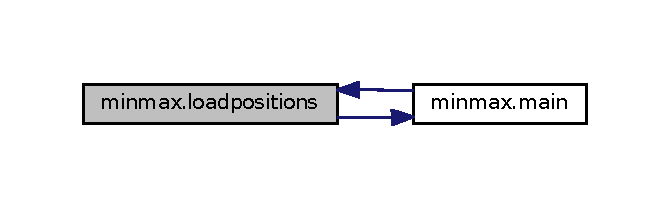
\includegraphics[width=322pt]{namespaceminmax_a702e9694cfedee3e80d21b70981aa0e3_cgraph}
\end{center}
\end{figure}


\hypertarget{namespaceminmax_ab99cb2d5b32e62e0cd3465a20b6683f8}{\index{minmax@{minmax}!main@{main}}
\index{main@{main}!minmax@{minmax}}
\subsubsection[{main}]{\setlength{\rightskip}{0pt plus 5cm}def minmax.\-main (
\begin{DoxyParamCaption}
\item[{}]{argv}
\end{DoxyParamCaption}
)}}\label{namespaceminmax_ab99cb2d5b32e62e0cd3465a20b6683f8}


Here is the call graph for this function\-:
\nopagebreak
\begin{figure}[H]
\begin{center}
\leavevmode
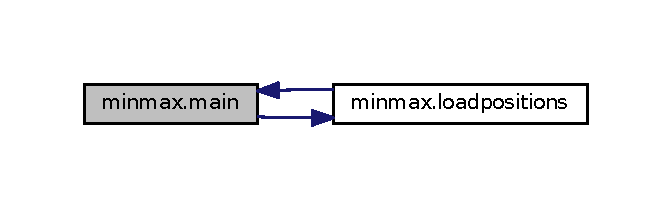
\includegraphics[width=322pt]{namespaceminmax_ab99cb2d5b32e62e0cd3465a20b6683f8_cgraph}
\end{center}
\end{figure}



\hypertarget{namespacenanoflann}{\section{nanoflann Namespace Reference}
\label{namespacenanoflann}\index{nanoflann@{nanoflann}}
}
\subsection*{Classes}
\begin{DoxyCompactItemize}
\item 
class \hyperlink{classnanoflann_1_1_k_n_n_result_set}{K\-N\-N\-Result\-Set}
\item 
class \hyperlink{classnanoflann_1_1_radius_result_set}{Radius\-Result\-Set}
\item 
struct \hyperlink{structnanoflann_1_1_index_dist___sorter}{Index\-Dist\-\_\-\-Sorter}
\item 
struct \hyperlink{structnanoflann_1_1_l1___adaptor}{L1\-\_\-\-Adaptor}
\item 
struct \hyperlink{structnanoflann_1_1_l2___adaptor}{L2\-\_\-\-Adaptor}
\item 
struct \hyperlink{structnanoflann_1_1_l2___simple___adaptor}{L2\-\_\-\-Simple\-\_\-\-Adaptor}
\item 
struct \hyperlink{structnanoflann_1_1metric___l1}{metric\-\_\-\-L1}
\item 
struct \hyperlink{structnanoflann_1_1metric___l2}{metric\-\_\-\-L2}
\item 
struct \hyperlink{structnanoflann_1_1metric___l2___simple}{metric\-\_\-\-L2\-\_\-\-Simple}
\item 
struct \hyperlink{structnanoflann_1_1_k_d_tree_single_index_adaptor_params}{K\-D\-Tree\-Single\-Index\-Adaptor\-Params}
\item 
struct \hyperlink{structnanoflann_1_1_search_params}{Search\-Params}
\item 
class \hyperlink{classnanoflann_1_1_pooled_allocator}{Pooled\-Allocator}
\item 
class \hyperlink{classnanoflann_1_1_k_d_tree_single_index_adaptor}{K\-D\-Tree\-Single\-Index\-Adaptor}
\item 
struct \hyperlink{structnanoflann_1_1_k_d_tree_eigen_matrix_adaptor}{K\-D\-Tree\-Eigen\-Matrix\-Adaptor}
\end{DoxyCompactItemize}
\subsection*{Functions}
\begin{DoxyCompactItemize}
\item 
{\footnotesize template$<$typename T $>$ }\\void \hyperlink{group__loadsave__grp_gadf909159ea32f125f71328d00ac2de8d}{save\-\_\-value} (F\-I\-L\-E $\ast$stream, const T \&value, size\-\_\-t count=1)
\item 
{\footnotesize template$<$typename T $>$ }\\void \hyperlink{group__loadsave__grp_gac767ee9c25febe0cd6af3ac2e186ffe7}{save\-\_\-value} (F\-I\-L\-E $\ast$stream, const std\-::vector$<$ T $>$ \&value)
\item 
{\footnotesize template$<$typename T $>$ }\\void \hyperlink{group__loadsave__grp_ga81940cd63b9ae619251d612d0ddbc819}{load\-\_\-value} (F\-I\-L\-E $\ast$stream, T \&value, size\-\_\-t count=1)
\item 
{\footnotesize template$<$typename T $>$ }\\void \hyperlink{group__loadsave__grp_gaefed46e8576d6ce3f1796bb13387ad3d}{load\-\_\-value} (F\-I\-L\-E $\ast$stream, std\-::vector$<$ T $>$ \&value)
\item 
{\footnotesize template$<$typename T $>$ }\\T \hyperlink{group__metric__grp_gaf15608f8914516f8d949a8c053d55021}{abs} (T x)
\item 
{\footnotesize template$<$$>$ }\\int \hyperlink{group__metric__grp_ga5c50e8d34773da556210ad34d6157763}{abs$<$ int $>$} (int x)
\item 
{\footnotesize template$<$$>$ }\\float \hyperlink{group__metric__grp_ga3c252a1b86662381fd025b0576124c2d}{abs$<$ float $>$} (float x)
\item 
{\footnotesize template$<$$>$ }\\double \hyperlink{group__metric__grp_ga3fb0513e5af33647f17713a36b10f156}{abs$<$ double $>$} (double x)
\item 
{\footnotesize template$<$$>$ }\\long double \hyperlink{group__metric__grp_ga02cfdf1bf211628b049ffd239a26e57e}{abs$<$ long double $>$} (long double x)
\item 
{\footnotesize template$<$typename T $>$ }\\T $\ast$ \hyperlink{group__memalloc__grp_ga477667da2a8edb1d65f5a7eebaffc1eb}{allocate} (size\-\_\-t count=1)
\end{DoxyCompactItemize}
\subsection*{Variables}
\begin{DoxyCompactItemize}
\item 
const size\-\_\-t \hyperlink{group__memalloc__grp_ga40956ef8f797399b4f478df9fc1566f4}{W\-O\-R\-D\-S\-I\-Z\-E} =16
\item 
const size\-\_\-t \hyperlink{group__memalloc__grp_gaf4df087b6f47e514f6062f7ada2d19d7}{B\-L\-O\-C\-K\-S\-I\-Z\-E} =8192
\end{DoxyCompactItemize}

\chapter{Class Documentation}
\hypertarget{classccmc_1_1_adapt3_d}{\section{ccmc\-:\-:Adapt3\-D Class Reference}
\label{classccmc_1_1_adapt3_d}\index{ccmc\-::\-Adapt3\-D@{ccmc\-::\-Adapt3\-D}}
}


T\-O\-D\-O\-: brief description of \hyperlink{classccmc_1_1_adapt3_d}{Adapt3\-D} class.  




{\ttfamily \#include $<$Adapt3\-D.\-h$>$}



Inheritance diagram for ccmc\-:\-:Adapt3\-D\-:\nopagebreak
\begin{figure}[H]
\begin{center}
\leavevmode
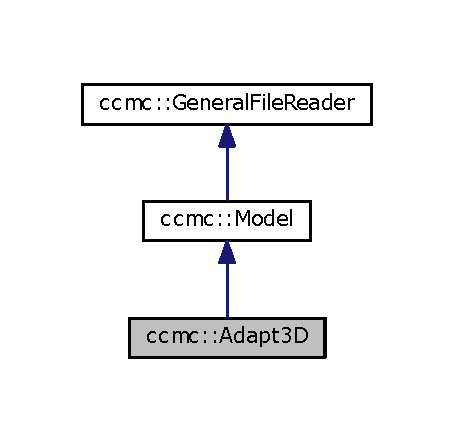
\includegraphics[width=218pt]{classccmc_1_1_adapt3_d__inherit__graph}
\end{center}
\end{figure}


Collaboration diagram for ccmc\-:\-:Adapt3\-D\-:\nopagebreak
\begin{figure}[H]
\begin{center}
\leavevmode
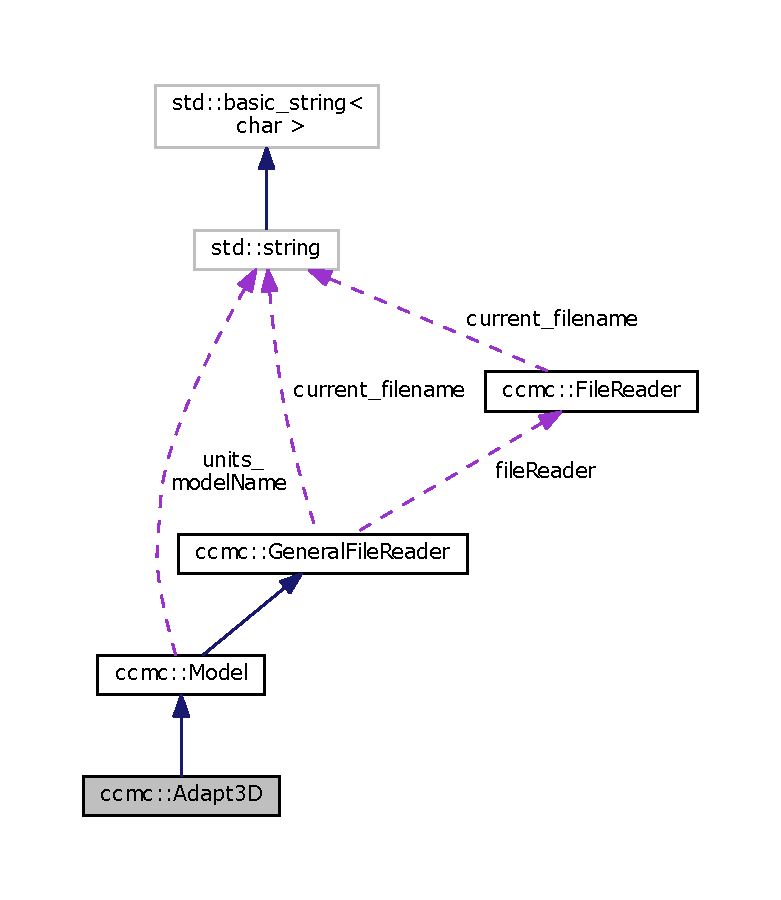
\includegraphics[width=350pt]{classccmc_1_1_adapt3_d__coll__graph}
\end{center}
\end{figure}
\subsection*{Public Member Functions}
\begin{DoxyCompactItemize}
\item 
\hyperlink{classccmc_1_1_adapt3_d_aa3927c68c63cde9e4006c0f8687116cb}{Adapt3\-D} ()
\item 
long \hyperlink{classccmc_1_1_adapt3_d_a02a5f2b5ba26cacd93f7c41c68c4b24a}{open} (const std\-::string \&filename)
\begin{DoxyCompactList}\small\item\em Opens a file.  \end{DoxyCompactList}\item 
\hyperlink{classccmc_1_1_interpolator}{Interpolator} $\ast$ \hyperlink{classccmc_1_1_adapt3_d_a4a82029cb4669a788c7ffa555fa4c20f}{create\-New\-Interpolator} ()
\begin{DoxyCompactList}\small\item\em Returns an \hyperlink{classccmc_1_1_interpolator}{Interpolator} object for the currently opened file.  \end{DoxyCompactList}\item 
\hyperlink{structccmc_1_1_smart_grid_search_values}{Smart\-Grid\-Search\-Values} $\ast$ \hyperlink{classccmc_1_1_adapt3_d_aba33c6663d647dc3d00e9007c909a7ed}{get\-Smart\-Grid\-Search\-Values} ()
\item 
const std\-::vector$<$ std\-::string $>$ \hyperlink{classccmc_1_1_adapt3_d_a0e69d88334151e8ac9b2cbb7dc546e64}{get\-Loaded\-Variables} ()
\begin{DoxyCompactList}\small\item\em Returns the list of variables that have been loaded into memory, using the load\-Variable or load\-Vector\-Variable methods. \end{DoxyCompactList}\item 
virtual \hyperlink{classccmc_1_1_adapt3_d_ac27c4556b1091bf63e5931ecadb37462}{$\sim$\-Adapt3\-D} ()
\end{DoxyCompactItemize}
\subsection*{Protected Member Functions}
\begin{DoxyCompactItemize}
\item 
void \hyperlink{classccmc_1_1_adapt3_d_aa4f0803514d069d146fdf58691b82d7a}{initialize\-Conversion\-Factors\-To\-S\-I} ()
\begin{DoxyCompactList}\small\item\em Initializes the conversion\-Factors\-To\-S\-I map.  \end{DoxyCompactList}\item 
void \hyperlink{classccmc_1_1_adapt3_d_a00d25fcceb69cc274df1c5e671f620e5}{initialize\-S\-I\-Units} ()
\begin{DoxyCompactList}\small\item\em Initializes the variable\-S\-I\-Units map.  \end{DoxyCompactList}\end{DoxyCompactItemize}
\subsection*{Additional Inherited Members}


\subsection{Detailed Description}
T\-O\-D\-O\-: brief description of \hyperlink{classccmc_1_1_adapt3_d}{Adapt3\-D} class. 

T\-O\-D\-O\-: full description of \hyperlink{classccmc_1_1_adapt3_d}{Adapt3\-D} class 

\subsection{Constructor \& Destructor Documentation}
\hypertarget{classccmc_1_1_adapt3_d_aa3927c68c63cde9e4006c0f8687116cb}{\index{ccmc\-::\-Adapt3\-D@{ccmc\-::\-Adapt3\-D}!Adapt3\-D@{Adapt3\-D}}
\index{Adapt3\-D@{Adapt3\-D}!ccmc::Adapt3D@{ccmc\-::\-Adapt3\-D}}
\subsubsection[{Adapt3\-D}]{\setlength{\rightskip}{0pt plus 5cm}ccmc\-::\-Adapt3\-D\-::\-Adapt3\-D (
\begin{DoxyParamCaption}
{}
\end{DoxyParamCaption}
)}}\label{classccmc_1_1_adapt3_d_aa3927c68c63cde9e4006c0f8687116cb}
Default constructor \hypertarget{classccmc_1_1_adapt3_d_ac27c4556b1091bf63e5931ecadb37462}{\index{ccmc\-::\-Adapt3\-D@{ccmc\-::\-Adapt3\-D}!$\sim$\-Adapt3\-D@{$\sim$\-Adapt3\-D}}
\index{$\sim$\-Adapt3\-D@{$\sim$\-Adapt3\-D}!ccmc::Adapt3D@{ccmc\-::\-Adapt3\-D}}
\subsubsection[{$\sim$\-Adapt3\-D}]{\setlength{\rightskip}{0pt plus 5cm}ccmc\-::\-Adapt3\-D\-::$\sim$\-Adapt3\-D (
\begin{DoxyParamCaption}
{}
\end{DoxyParamCaption}
)\hspace{0.3cm}{\ttfamily [virtual]}}}\label{classccmc_1_1_adapt3_d_ac27c4556b1091bf63e5931ecadb37462}
Destructor 

\subsection{Member Function Documentation}
\hypertarget{classccmc_1_1_adapt3_d_a4a82029cb4669a788c7ffa555fa4c20f}{\index{ccmc\-::\-Adapt3\-D@{ccmc\-::\-Adapt3\-D}!create\-New\-Interpolator@{create\-New\-Interpolator}}
\index{create\-New\-Interpolator@{create\-New\-Interpolator}!ccmc::Adapt3D@{ccmc\-::\-Adapt3\-D}}
\subsubsection[{create\-New\-Interpolator}]{\setlength{\rightskip}{0pt plus 5cm}{\bf Interpolator} $\ast$ ccmc\-::\-Adapt3\-D\-::create\-New\-Interpolator (
\begin{DoxyParamCaption}
{}
\end{DoxyParamCaption}
)\hspace{0.3cm}{\ttfamily [virtual]}}}\label{classccmc_1_1_adapt3_d_a4a82029cb4669a788c7ffa555fa4c20f}


Returns an \hyperlink{classccmc_1_1_interpolator}{Interpolator} object for the currently opened file.  

This returns an \hyperlink{classccmc_1_1_interpolator}{Interpolator} object that contains all the necessary local variables required to interpolate independent of any other \hyperlink{classccmc_1_1_interpolator}{Interpolator} object. The pointer must be deleted from the calling program. \begin{DoxyReturn}{Returns}
A pointer to an \hyperlink{classccmc_1_1_interpolator}{Interpolator} object. 
\end{DoxyReturn}
 

Implements \hyperlink{classccmc_1_1_model_a0dd491507c14502c27aa61b020fca8cc}{ccmc\-::\-Model}.

\hypertarget{classccmc_1_1_adapt3_d_a0e69d88334151e8ac9b2cbb7dc546e64}{\index{ccmc\-::\-Adapt3\-D@{ccmc\-::\-Adapt3\-D}!get\-Loaded\-Variables@{get\-Loaded\-Variables}}
\index{get\-Loaded\-Variables@{get\-Loaded\-Variables}!ccmc::Adapt3D@{ccmc\-::\-Adapt3\-D}}
\subsubsection[{get\-Loaded\-Variables}]{\setlength{\rightskip}{0pt plus 5cm}const std\-::vector$<$ std\-::string $>$ ccmc\-::\-Adapt3\-D\-::get\-Loaded\-Variables (
\begin{DoxyParamCaption}
{}
\end{DoxyParamCaption}
)\hspace{0.3cm}{\ttfamily [virtual]}}}\label{classccmc_1_1_adapt3_d_a0e69d88334151e8ac9b2cbb7dc546e64}


Returns the list of variables that have been loaded into memory, using the load\-Variable or load\-Vector\-Variable methods. 



Reimplemented from \hyperlink{classccmc_1_1_model_ac49a0eec99d25e9ed08ffff959e4ecdc}{ccmc\-::\-Model}.



Here is the call graph for this function\-:\nopagebreak
\begin{figure}[H]
\begin{center}
\leavevmode
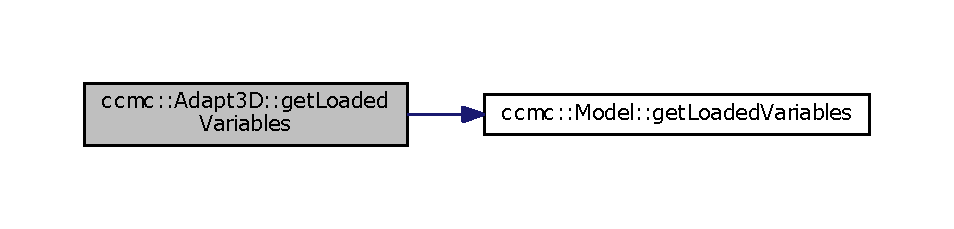
\includegraphics[width=350pt]{classccmc_1_1_adapt3_d_a0e69d88334151e8ac9b2cbb7dc546e64_cgraph}
\end{center}
\end{figure}


\hypertarget{classccmc_1_1_adapt3_d_aba33c6663d647dc3d00e9007c909a7ed}{\index{ccmc\-::\-Adapt3\-D@{ccmc\-::\-Adapt3\-D}!get\-Smart\-Grid\-Search\-Values@{get\-Smart\-Grid\-Search\-Values}}
\index{get\-Smart\-Grid\-Search\-Values@{get\-Smart\-Grid\-Search\-Values}!ccmc::Adapt3D@{ccmc\-::\-Adapt3\-D}}
\subsubsection[{get\-Smart\-Grid\-Search\-Values}]{\setlength{\rightskip}{0pt plus 5cm}{\bf Smart\-Grid\-Search\-Values} $\ast$ ccmc\-::\-Adapt3\-D\-::get\-Smart\-Grid\-Search\-Values (
\begin{DoxyParamCaption}
{}
\end{DoxyParamCaption}
)}}\label{classccmc_1_1_adapt3_d_aba33c6663d647dc3d00e9007c909a7ed}
\hypertarget{classccmc_1_1_adapt3_d_aa4f0803514d069d146fdf58691b82d7a}{\index{ccmc\-::\-Adapt3\-D@{ccmc\-::\-Adapt3\-D}!initialize\-Conversion\-Factors\-To\-S\-I@{initialize\-Conversion\-Factors\-To\-S\-I}}
\index{initialize\-Conversion\-Factors\-To\-S\-I@{initialize\-Conversion\-Factors\-To\-S\-I}!ccmc::Adapt3D@{ccmc\-::\-Adapt3\-D}}
\subsubsection[{initialize\-Conversion\-Factors\-To\-S\-I}]{\setlength{\rightskip}{0pt plus 5cm}void ccmc\-::\-Adapt3\-D\-::initialize\-Conversion\-Factors\-To\-S\-I (
\begin{DoxyParamCaption}
{}
\end{DoxyParamCaption}
)\hspace{0.3cm}{\ttfamily [protected]}, {\ttfamily [virtual]}}}\label{classccmc_1_1_adapt3_d_aa4f0803514d069d146fdf58691b82d7a}


Initializes the conversion\-Factors\-To\-S\-I map.  

These factors are used to convert interpolated values to S\-I units.  T\-O\-D\-O\-: fix these conversion factors

Implements \hyperlink{classccmc_1_1_model_a6f04326691fba448e2cfb7c7ab90a45a}{ccmc\-::\-Model}.

\hypertarget{classccmc_1_1_adapt3_d_a00d25fcceb69cc274df1c5e671f620e5}{\index{ccmc\-::\-Adapt3\-D@{ccmc\-::\-Adapt3\-D}!initialize\-S\-I\-Units@{initialize\-S\-I\-Units}}
\index{initialize\-S\-I\-Units@{initialize\-S\-I\-Units}!ccmc::Adapt3D@{ccmc\-::\-Adapt3\-D}}
\subsubsection[{initialize\-S\-I\-Units}]{\setlength{\rightskip}{0pt plus 5cm}void ccmc\-::\-Adapt3\-D\-::initialize\-S\-I\-Units (
\begin{DoxyParamCaption}
{}
\end{DoxyParamCaption}
)\hspace{0.3cm}{\ttfamily [protected]}, {\ttfamily [virtual]}}}\label{classccmc_1_1_adapt3_d_a00d25fcceb69cc274df1c5e671f620e5}


Initializes the variable\-S\-I\-Units map.  



Implements \hyperlink{classccmc_1_1_model_a68d31e8d8cce59269c994de25d048178}{ccmc\-::\-Model}.

\hypertarget{classccmc_1_1_adapt3_d_a02a5f2b5ba26cacd93f7c41c68c4b24a}{\index{ccmc\-::\-Adapt3\-D@{ccmc\-::\-Adapt3\-D}!open@{open}}
\index{open@{open}!ccmc::Adapt3D@{ccmc\-::\-Adapt3\-D}}
\subsubsection[{open}]{\setlength{\rightskip}{0pt plus 5cm}long ccmc\-::\-Adapt3\-D\-::open (
\begin{DoxyParamCaption}
\item[{const std\-::string \&}]{filename}
\end{DoxyParamCaption}
)\hspace{0.3cm}{\ttfamily [virtual]}}}\label{classccmc_1_1_adapt3_d_a02a5f2b5ba26cacd93f7c41c68c4b24a}


Opens a file.  

Opens a file and performs any necessary initialization required to work with the data. 
\begin{DoxyParams}{Parameters}
{\em filename} & \\
\hline
\end{DoxyParams}
 

Implements \hyperlink{classccmc_1_1_model_a3c64dc635c2c1a2fe2f8efa2a3666282}{ccmc\-::\-Model}.



Here is the call graph for this function\-:\nopagebreak
\begin{figure}[H]
\begin{center}
\leavevmode
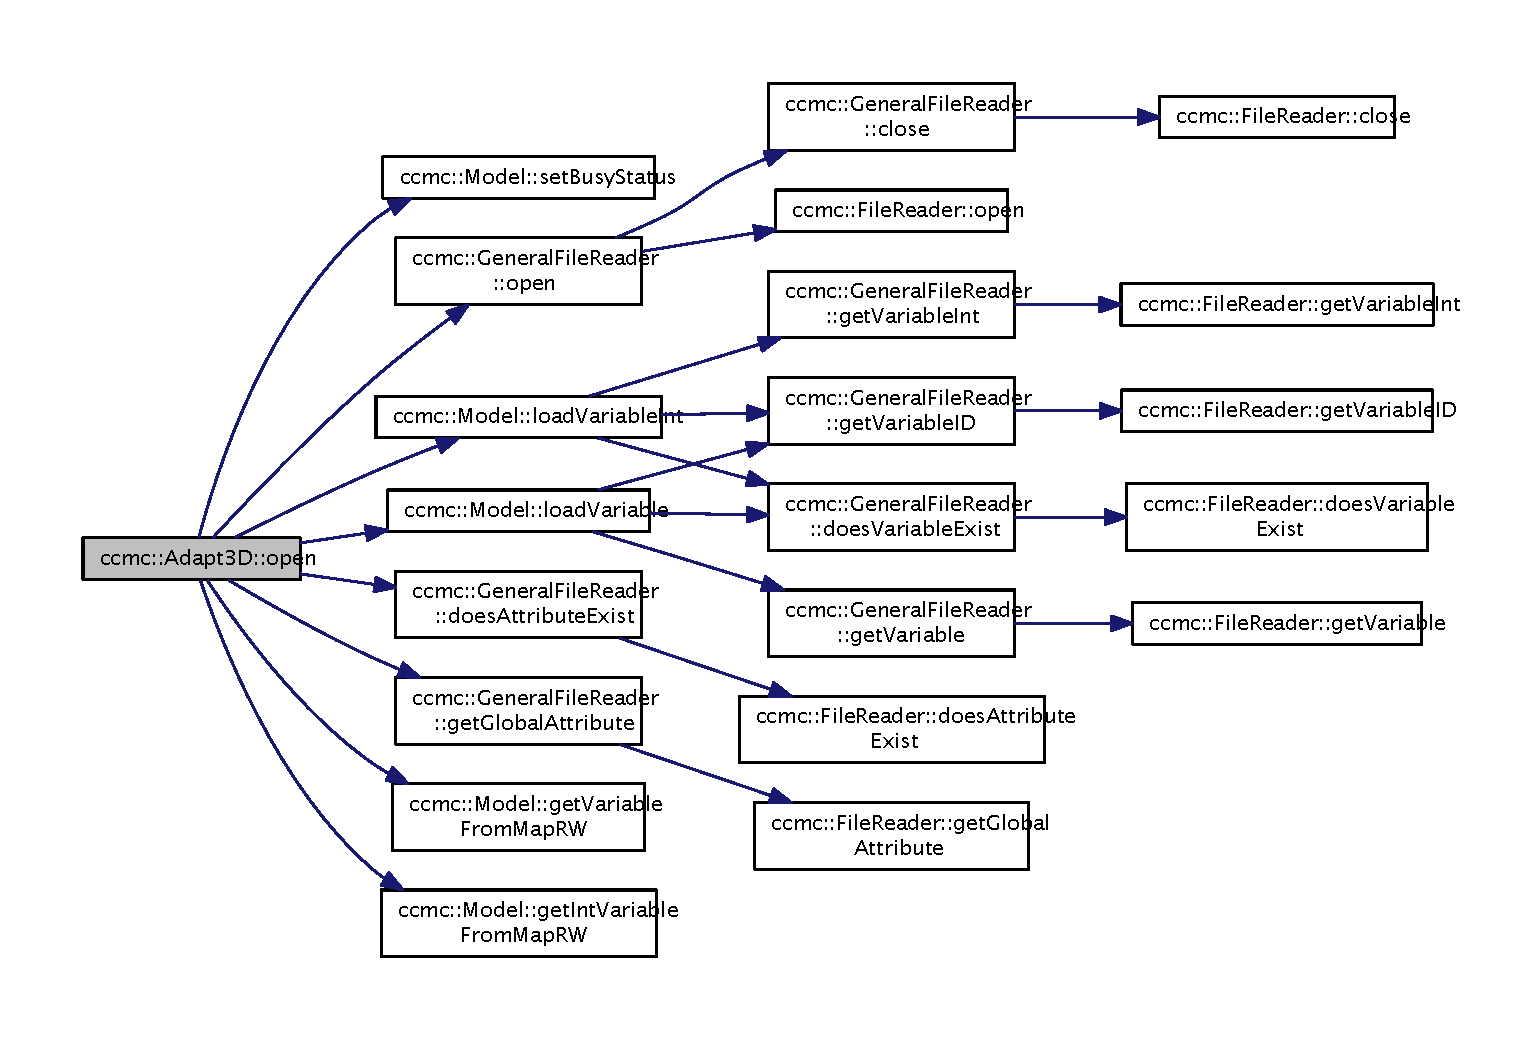
\includegraphics[width=350pt]{classccmc_1_1_adapt3_d_a02a5f2b5ba26cacd93f7c41c68c4b24a_cgraph}
\end{center}
\end{figure}




The documentation for this class was generated from the following files\-:\begin{DoxyCompactItemize}
\item 
/\-Users/apembrok/\-Documents/workspaces/workspace.\-bak2/workspace.\-backup/kameleon-\/plus/src/ccmc/\hyperlink{_adapt3_d_8h}{Adapt3\-D.\-h}\item 
/\-Users/apembrok/\-Documents/workspaces/workspace.\-bak2/workspace.\-backup/kameleon-\/plus/src/ccmc/\hyperlink{_adapt3_d_8cpp}{Adapt3\-D.\-cpp}\end{DoxyCompactItemize}

\hypertarget{classccmc_1_1_adapt3_d_interpolator}{\section{ccmc\-:\-:Adapt3\-D\-Interpolator Class Reference}
\label{classccmc_1_1_adapt3_d_interpolator}\index{ccmc\-::\-Adapt3\-D\-Interpolator@{ccmc\-::\-Adapt3\-D\-Interpolator}}
}


T\-O\-D\-O\-: brief description of \hyperlink{classccmc_1_1_b_a_t_s_r_u_s_interpolator}{B\-A\-T\-S\-R\-U\-S\-Interpolator} class.  




{\ttfamily \#include $<$Adapt3\-D\-Interpolator.\-h$>$}



Inheritance diagram for ccmc\-:\-:Adapt3\-D\-Interpolator\-:\nopagebreak
\begin{figure}[H]
\begin{center}
\leavevmode
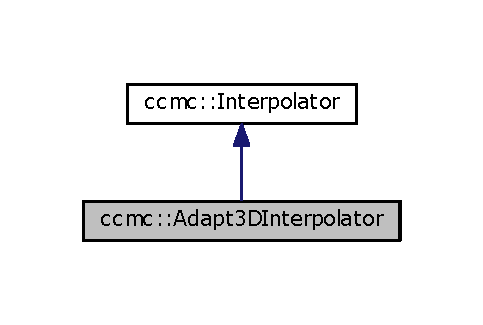
\includegraphics[width=232pt]{classccmc_1_1_adapt3_d_interpolator__inherit__graph}
\end{center}
\end{figure}


Collaboration diagram for ccmc\-:\-:Adapt3\-D\-Interpolator\-:\nopagebreak
\begin{figure}[H]
\begin{center}
\leavevmode
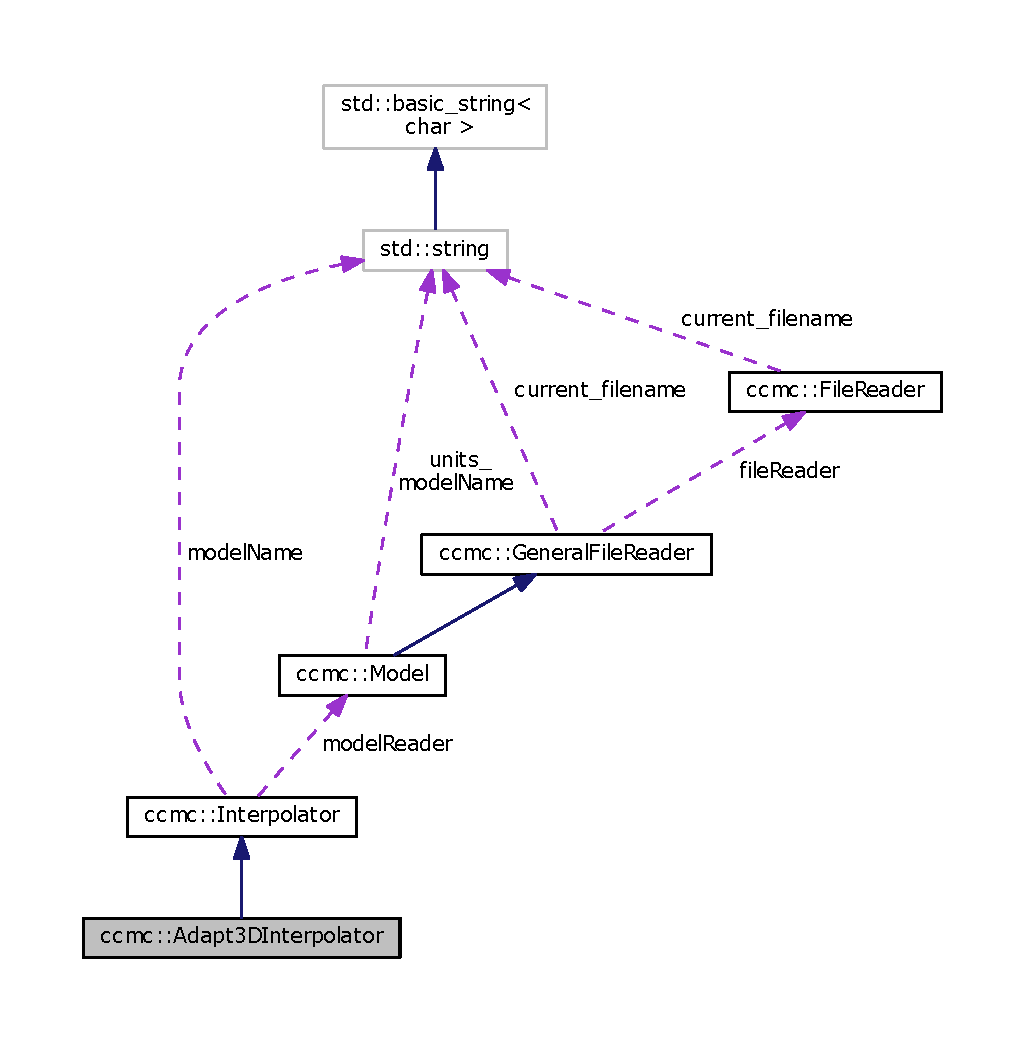
\includegraphics[width=350pt]{classccmc_1_1_adapt3_d_interpolator__coll__graph}
\end{center}
\end{figure}
\subsection*{Public Member Functions}
\begin{DoxyCompactItemize}
\item 
\hyperlink{classccmc_1_1_adapt3_d_interpolator_a79b9d9e9cbfc04e72d34c0853d916514}{Adapt3\-D\-Interpolator} (\hyperlink{classccmc_1_1_model}{Model} $\ast$\hyperlink{classccmc_1_1_interpolator_afee5bb61e5d5a0a7b9152c6f74378c4a}{model\-Reader})
\item 
float \hyperlink{classccmc_1_1_adapt3_d_interpolator_aecaa97aad175a8696d8351607a08158c}{interpolate} (const std\-::string \&, const float \&c0, const float \&c1, const float \&c2)
\item 
float \hyperlink{classccmc_1_1_adapt3_d_interpolator_ab9a45aa8feb07a6d55e45da3d202060c}{interpolate} (const std\-::string \&, const float \&c0, const float \&c1, const float \&c2, float \&dc0, float \&dc1, float \&dc2)
\item 
float \hyperlink{classccmc_1_1_adapt3_d_interpolator_ad6f6e98e2070f7bf9f99be40c127548f}{interpolate} (const long \&variable\-\_\-id, const float \&c0, const float \&c1, const float \&c2)
\item 
float \hyperlink{classccmc_1_1_adapt3_d_interpolator_a62f9740d20678b993f2871c6505f7df3}{interpolate} (const long \&variable\-\_\-id, const float \&c0, const float \&c1, const float \&c2, float \&dc0, float \&dc1, float \&dc2)
\item 
virtual \hyperlink{classccmc_1_1_adapt3_d_interpolator_a43116c61408cf05876999e2c2f1f67fb}{$\sim$\-Adapt3\-D\-Interpolator} ()
\end{DoxyCompactItemize}
\subsection*{Static Public Member Functions}
\begin{DoxyCompactItemize}
\item 
static void \hyperlink{classccmc_1_1_adapt3_d_interpolator_ad041ba3c92e7f5b0b1f3ede0bd9ec7cb}{calculation1} (const float \&a, const float \&b, const float \&c, const float \&d, const float \&e, float \&result)
\end{DoxyCompactItemize}
\subsection*{Additional Inherited Members}


\subsection{Detailed Description}
T\-O\-D\-O\-: brief description of \hyperlink{classccmc_1_1_b_a_t_s_r_u_s_interpolator}{B\-A\-T\-S\-R\-U\-S\-Interpolator} class. 

T\-O\-D\-O\-: full description of \hyperlink{classccmc_1_1_b_a_t_s_r_u_s_interpolator}{B\-A\-T\-S\-R\-U\-S\-Interpolator} class 

\subsection{Constructor \& Destructor Documentation}
\hypertarget{classccmc_1_1_adapt3_d_interpolator_a79b9d9e9cbfc04e72d34c0853d916514}{\index{ccmc\-::\-Adapt3\-D\-Interpolator@{ccmc\-::\-Adapt3\-D\-Interpolator}!Adapt3\-D\-Interpolator@{Adapt3\-D\-Interpolator}}
\index{Adapt3\-D\-Interpolator@{Adapt3\-D\-Interpolator}!ccmc::Adapt3DInterpolator@{ccmc\-::\-Adapt3\-D\-Interpolator}}
\subsubsection[{Adapt3\-D\-Interpolator}]{\setlength{\rightskip}{0pt plus 5cm}ccmc\-::\-Adapt3\-D\-Interpolator\-::\-Adapt3\-D\-Interpolator (
\begin{DoxyParamCaption}
\item[{{\bf Model} $\ast$}]{model\-Reader}
\end{DoxyParamCaption}
)}}\label{classccmc_1_1_adapt3_d_interpolator_a79b9d9e9cbfc04e72d34c0853d916514}

\begin{DoxyParams}{Parameters}
{\em model\-Reader} & Pointer to the \hyperlink{classccmc_1_1_model}{Model} object containing the appropriate variable maps. \hyperlink{classccmc_1_1_adapt3_d_interpolator}{Adapt3\-D\-Interpolator} should be returned by a \hyperlink{classccmc_1_1_adapt3_d_a4a82029cb4669a788c7ffa555fa4c20f}{Adapt3\-D\-::create\-New\-Interpolator()} call. \\
\hline
\end{DoxyParams}


Here is the call graph for this function\-:\nopagebreak
\begin{figure}[H]
\begin{center}
\leavevmode
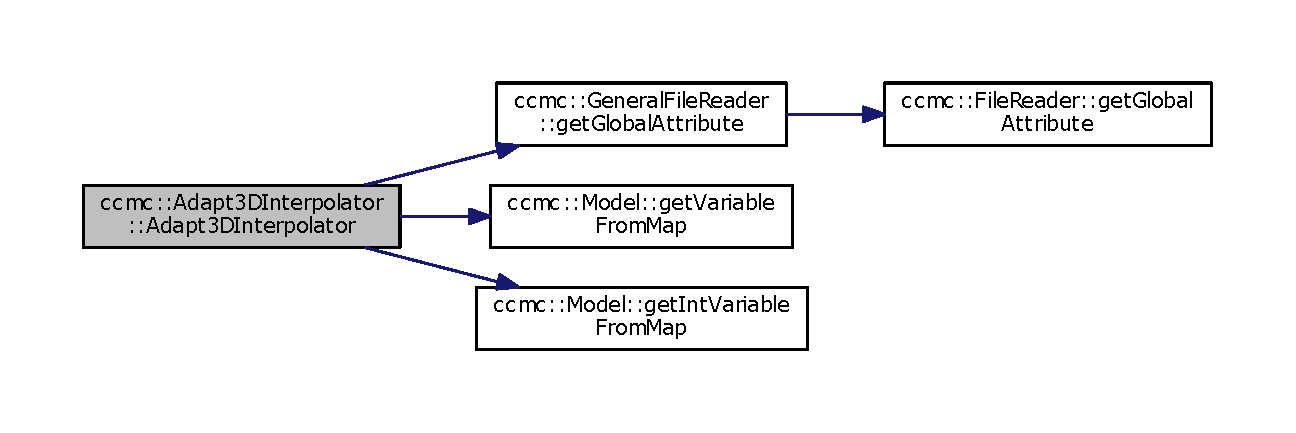
\includegraphics[width=350pt]{classccmc_1_1_adapt3_d_interpolator_a79b9d9e9cbfc04e72d34c0853d916514_cgraph}
\end{center}
\end{figure}


\hypertarget{classccmc_1_1_adapt3_d_interpolator_a43116c61408cf05876999e2c2f1f67fb}{\index{ccmc\-::\-Adapt3\-D\-Interpolator@{ccmc\-::\-Adapt3\-D\-Interpolator}!$\sim$\-Adapt3\-D\-Interpolator@{$\sim$\-Adapt3\-D\-Interpolator}}
\index{$\sim$\-Adapt3\-D\-Interpolator@{$\sim$\-Adapt3\-D\-Interpolator}!ccmc::Adapt3DInterpolator@{ccmc\-::\-Adapt3\-D\-Interpolator}}
\subsubsection[{$\sim$\-Adapt3\-D\-Interpolator}]{\setlength{\rightskip}{0pt plus 5cm}ccmc\-::\-Adapt3\-D\-Interpolator\-::$\sim$\-Adapt3\-D\-Interpolator (
\begin{DoxyParamCaption}
{}
\end{DoxyParamCaption}
)\hspace{0.3cm}{\ttfamily [virtual]}}}\label{classccmc_1_1_adapt3_d_interpolator_a43116c61408cf05876999e2c2f1f67fb}
Destructor 

\subsection{Member Function Documentation}
\hypertarget{classccmc_1_1_adapt3_d_interpolator_ad041ba3c92e7f5b0b1f3ede0bd9ec7cb}{\index{ccmc\-::\-Adapt3\-D\-Interpolator@{ccmc\-::\-Adapt3\-D\-Interpolator}!calculation1@{calculation1}}
\index{calculation1@{calculation1}!ccmc::Adapt3DInterpolator@{ccmc\-::\-Adapt3\-D\-Interpolator}}
\subsubsection[{calculation1}]{\setlength{\rightskip}{0pt plus 5cm}void ccmc\-::\-Adapt3\-D\-Interpolator\-::calculation1 (
\begin{DoxyParamCaption}
\item[{const float \&}]{a, }
\item[{const float \&}]{b, }
\item[{const float \&}]{c, }
\item[{const float \&}]{d, }
\item[{const float \&}]{e, }
\item[{float \&}]{result}
\end{DoxyParamCaption}
)\hspace{0.3cm}{\ttfamily [static]}}}\label{classccmc_1_1_adapt3_d_interpolator_ad041ba3c92e7f5b0b1f3ede0bd9ec7cb}
\hypertarget{classccmc_1_1_adapt3_d_interpolator_aecaa97aad175a8696d8351607a08158c}{\index{ccmc\-::\-Adapt3\-D\-Interpolator@{ccmc\-::\-Adapt3\-D\-Interpolator}!interpolate@{interpolate}}
\index{interpolate@{interpolate}!ccmc::Adapt3DInterpolator@{ccmc\-::\-Adapt3\-D\-Interpolator}}
\subsubsection[{interpolate}]{\setlength{\rightskip}{0pt plus 5cm}float ccmc\-::\-Adapt3\-D\-Interpolator\-::interpolate (
\begin{DoxyParamCaption}
\item[{const std\-::string \&}]{variable, }
\item[{const float \&}]{c0, }
\item[{const float \&}]{c1, }
\item[{const float \&}]{c2}
\end{DoxyParamCaption}
)\hspace{0.3cm}{\ttfamily [virtual]}}}\label{classccmc_1_1_adapt3_d_interpolator_aecaa97aad175a8696d8351607a08158c}

\begin{DoxyParams}{Parameters}
{\em variable} & \\
\hline
{\em c0} & X component of the position \\
\hline
{\em c1} & Y component of the position \\
\hline
{\em c2} & Z component of the position \\
\hline
\end{DoxyParams}
\begin{DoxyReturn}{Returns}

\end{DoxyReturn}


Implements \hyperlink{classccmc_1_1_interpolator_ad5c1dd3693f83d75a2335b7c28cd649d}{ccmc\-::\-Interpolator}.

\hypertarget{classccmc_1_1_adapt3_d_interpolator_ab9a45aa8feb07a6d55e45da3d202060c}{\index{ccmc\-::\-Adapt3\-D\-Interpolator@{ccmc\-::\-Adapt3\-D\-Interpolator}!interpolate@{interpolate}}
\index{interpolate@{interpolate}!ccmc::Adapt3DInterpolator@{ccmc\-::\-Adapt3\-D\-Interpolator}}
\subsubsection[{interpolate}]{\setlength{\rightskip}{0pt plus 5cm}float ccmc\-::\-Adapt3\-D\-Interpolator\-::interpolate (
\begin{DoxyParamCaption}
\item[{const std\-::string \&}]{variable, }
\item[{const float \&}]{c0, }
\item[{const float \&}]{c1, }
\item[{const float \&}]{c2, }
\item[{float \&}]{dc0, }
\item[{float \&}]{dc1, }
\item[{float \&}]{dc2}
\end{DoxyParamCaption}
)\hspace{0.3cm}{\ttfamily [virtual]}}}\label{classccmc_1_1_adapt3_d_interpolator_ab9a45aa8feb07a6d55e45da3d202060c}
Interpolation method. Note that using the variable I\-D is significantly faster than using the variable string. 
\begin{DoxyParams}{Parameters}
{\em variable} & The input variable. \\
\hline
{\em c0} & X component of the position \\
\hline
{\em c1} & Y component of the position \\
\hline
{\em c2} & Z component of the position \\
\hline
{\em dc0} & Reference to a variable to store the delta for component 0 \\
\hline
{\em dc1} & Reference to a variable to store the delta for component 1 \\
\hline
{\em dc2} & Reference to a variable to store the delta for component 2 \\
\hline
\end{DoxyParams}
\begin{DoxyReturn}{Returns}
The interpolated value at position (c0,c1,c2) with deltas (dc0,dc1,dc2) 
\end{DoxyReturn}
T\-O\-D\-O\-: figure out what to do about the dc0,dc1,dc2 values

lets see if required variables are in memory 

Implements \hyperlink{classccmc_1_1_interpolator_ae02453da5a1a8f472f33b2058424ddb6}{ccmc\-::\-Interpolator}.



Here is the call graph for this function\-:\nopagebreak
\begin{figure}[H]
\begin{center}
\leavevmode
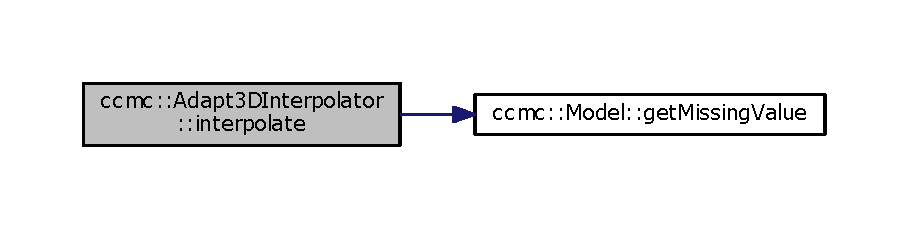
\includegraphics[width=350pt]{classccmc_1_1_adapt3_d_interpolator_ab9a45aa8feb07a6d55e45da3d202060c_cgraph}
\end{center}
\end{figure}


\hypertarget{classccmc_1_1_adapt3_d_interpolator_ad6f6e98e2070f7bf9f99be40c127548f}{\index{ccmc\-::\-Adapt3\-D\-Interpolator@{ccmc\-::\-Adapt3\-D\-Interpolator}!interpolate@{interpolate}}
\index{interpolate@{interpolate}!ccmc::Adapt3DInterpolator@{ccmc\-::\-Adapt3\-D\-Interpolator}}
\subsubsection[{interpolate}]{\setlength{\rightskip}{0pt plus 5cm}float ccmc\-::\-Adapt3\-D\-Interpolator\-::interpolate (
\begin{DoxyParamCaption}
\item[{const long \&}]{variable\-\_\-id, }
\item[{const float \&}]{c0, }
\item[{const float \&}]{c1, }
\item[{const float \&}]{c2}
\end{DoxyParamCaption}
)\hspace{0.3cm}{\ttfamily [virtual]}}}\label{classccmc_1_1_adapt3_d_interpolator_ad6f6e98e2070f7bf9f99be40c127548f}

\begin{DoxyParams}{Parameters}
{\em variable\-\_\-id} & \\
\hline
{\em c0} & X component of the position \\
\hline
{\em c1} & Y component of the position \\
\hline
{\em c2} & Z component of the position \\
\hline
\end{DoxyParams}
\begin{DoxyReturn}{Returns}

\end{DoxyReturn}


Implements \hyperlink{classccmc_1_1_interpolator_a6bfe1b4075f03704b893bb96e1675a3b}{ccmc\-::\-Interpolator}.



Here is the call graph for this function\-:\nopagebreak
\begin{figure}[H]
\begin{center}
\leavevmode
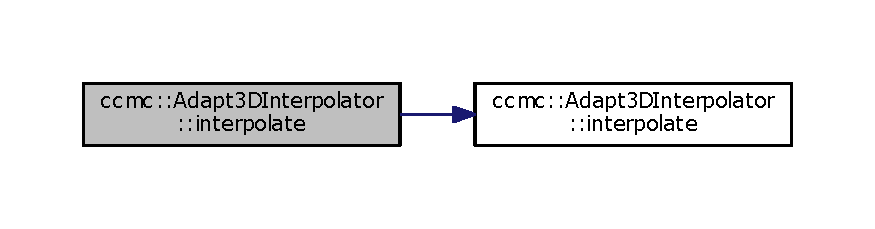
\includegraphics[width=350pt]{classccmc_1_1_adapt3_d_interpolator_ad6f6e98e2070f7bf9f99be40c127548f_cgraph}
\end{center}
\end{figure}


\hypertarget{classccmc_1_1_adapt3_d_interpolator_a62f9740d20678b993f2871c6505f7df3}{\index{ccmc\-::\-Adapt3\-D\-Interpolator@{ccmc\-::\-Adapt3\-D\-Interpolator}!interpolate@{interpolate}}
\index{interpolate@{interpolate}!ccmc::Adapt3DInterpolator@{ccmc\-::\-Adapt3\-D\-Interpolator}}
\subsubsection[{interpolate}]{\setlength{\rightskip}{0pt plus 5cm}float ccmc\-::\-Adapt3\-D\-Interpolator\-::interpolate (
\begin{DoxyParamCaption}
\item[{const long \&}]{variable\-\_\-id, }
\item[{const float \&}]{c0, }
\item[{const float \&}]{c1, }
\item[{const float \&}]{c2, }
\item[{float \&}]{dc0, }
\item[{float \&}]{dc1, }
\item[{float \&}]{dc2}
\end{DoxyParamCaption}
)\hspace{0.3cm}{\ttfamily [virtual]}}}\label{classccmc_1_1_adapt3_d_interpolator_a62f9740d20678b993f2871c6505f7df3}
Interpolation method. Note that using the variable I\-D is significantly faster than using the variable string. 
\begin{DoxyParams}{Parameters}
{\em variable\-\_\-id} & A long representing the variable I\-D. \\
\hline
{\em c0} & X component of the position \\
\hline
{\em c1} & Y component of the position \\
\hline
{\em c2} & Z component of the position \\
\hline
{\em dc0} & Reference to a variable to store the delta for component 0 \\
\hline
{\em dc1} & Reference to a variable to store the delta for component 1 \\
\hline
{\em dc2} & Reference to a variable to store the delta for component 2 \\
\hline
\end{DoxyParams}
\begin{DoxyReturn}{Returns}
The interpolated value at position (c0,c1,c2) with deltas (dc0,dc1,dc2) 
\end{DoxyReturn}


Implements \hyperlink{classccmc_1_1_interpolator_aa6b272bd53630020d92938ec1e5cfad9}{ccmc\-::\-Interpolator}.



Here is the call graph for this function\-:\nopagebreak
\begin{figure}[H]
\begin{center}
\leavevmode
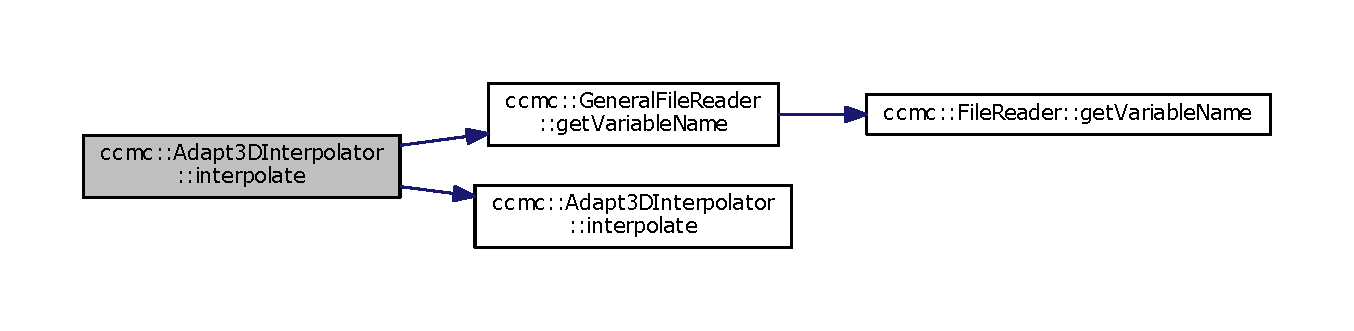
\includegraphics[width=350pt]{classccmc_1_1_adapt3_d_interpolator_a62f9740d20678b993f2871c6505f7df3_cgraph}
\end{center}
\end{figure}




The documentation for this class was generated from the following files\-:\begin{DoxyCompactItemize}
\item 
/\-Users/apembrok/\-Documents/workspaces/workspace.\-bak2/workspace.\-backup/kameleon-\/plus/src/ccmc/\hyperlink{_adapt3_d_interpolator_8h}{Adapt3\-D\-Interpolator.\-h}\item 
/\-Users/apembrok/\-Documents/workspaces/workspace.\-bak2/workspace.\-backup/kameleon-\/plus/src/ccmc/\hyperlink{_adapt3_d_interpolator_8cpp}{Adapt3\-D\-Interpolator.\-cpp}\end{DoxyCompactItemize}

\hypertarget{classccmc_1_1_attribute}{\section{ccmc\-:\-:Attribute Class Reference}
\label{classccmc_1_1_attribute}\index{ccmc\-::\-Attribute@{ccmc\-::\-Attribute}}
}


T\-O\-D\-O\-: brief description of \hyperlink{classccmc_1_1_attribute}{Attribute} class.  




{\ttfamily \#include $<$ccmc/\-Attribute.\-h$>$}

\subsection*{Public Types}
\begin{DoxyCompactItemize}
\item 
enum \hyperlink{classccmc_1_1_attribute_a4b2de185d21d77a8dd84ed192c08e6dc}{Attribute\-Type} \{ \hyperlink{classccmc_1_1_attribute_a4b2de185d21d77a8dd84ed192c08e6dca7d2598b6d93c726b54c97a0a69bf4d91}{F\-L\-O\-A\-T}, 
\hyperlink{classccmc_1_1_attribute_a4b2de185d21d77a8dd84ed192c08e6dcafc98ae76f4fe5d5f1f2ab252b372ca5f}{I\-N\-T}, 
\hyperlink{classccmc_1_1_attribute_a4b2de185d21d77a8dd84ed192c08e6dcaea0fc43df5a3bffd5e848ecfe252f306}{S\-T\-R\-I\-N\-G}
 \}
\end{DoxyCompactItemize}
\subsection*{Public Member Functions}
\begin{DoxyCompactItemize}
\item 
std\-::string \hyperlink{classccmc_1_1_attribute_a4c1cb6f974a0c9fcd301e5e1b522f01b}{get\-Attribute\-Name} ()
\item 
void \hyperlink{classccmc_1_1_attribute_a26894d09527f45cf5f43b799cbce6db1}{set\-Attribute\-Name} (std\-::string attribute\-Name)
\item 
void \hyperlink{classccmc_1_1_attribute_a8430f2e0b3fe3792e39132785ed87874}{set\-Attribute\-Value} (std\-::string \&value)
\item 
void \hyperlink{classccmc_1_1_attribute_adcc682edbbbf610424e559d47d0fe7e8}{set\-Attribute\-Value} (int \&value)
\item 
void \hyperlink{classccmc_1_1_attribute_a27e391143448b28032c6920fe2882142}{set\-Attribute\-Value} (float \&value)
\item 
\hyperlink{classccmc_1_1_attribute_a4b2de185d21d77a8dd84ed192c08e6dc}{Attribute\-Type} \hyperlink{classccmc_1_1_attribute_a47369f077a44690c3a0cc99cc2a40142}{get\-Attribute\-Type} ()
\item 
float \hyperlink{classccmc_1_1_attribute_a58c473ab213fc55f6f68f6fee311ec52}{get\-Attribute\-Float} ()
\item 
std\-::string \hyperlink{classccmc_1_1_attribute_ad1f07128784fe7f0416edc4a813ab1b6}{get\-Attribute\-String} ()
\item 
int \hyperlink{classccmc_1_1_attribute_af808a85742d9649cfe6fc218546303ac}{get\-Attribute\-Int} ()
\item 
\hyperlink{classccmc_1_1_attribute_abcb1a4d1ba3e9db38bda34410c3d6a6e}{Attribute} ()
\item 
std\-::string \hyperlink{classccmc_1_1_attribute_a8b5b6d5379f7b88cef4d79c2a494095d}{to\-String} () const 
\item 
virtual \hyperlink{classccmc_1_1_attribute_a38d5132b32554f2303d29f8f0e62e9b1}{$\sim$\-Attribute} ()
\end{DoxyCompactItemize}
\subsection*{Friends}
\begin{DoxyCompactItemize}
\item 
std\-::ostream \& \hyperlink{classccmc_1_1_attribute_a046dcd1efeb7b260e948652d8de23250}{operator$<$$<$} (std\-::ostream \&out, const \hyperlink{classccmc_1_1_attribute}{Attribute} attribute)
\end{DoxyCompactItemize}


\subsection{Detailed Description}
T\-O\-D\-O\-: brief description of \hyperlink{classccmc_1_1_attribute}{Attribute} class. 

T\-O\-D\-O\-: full description of \hyperlink{classccmc_1_1_attribute}{Attribute} class 

\subsection{Member Enumeration Documentation}
\hypertarget{classccmc_1_1_attribute_a4b2de185d21d77a8dd84ed192c08e6dc}{\index{ccmc\-::\-Attribute@{ccmc\-::\-Attribute}!Attribute\-Type@{Attribute\-Type}}
\index{Attribute\-Type@{Attribute\-Type}!ccmc::Attribute@{ccmc\-::\-Attribute}}
\subsubsection[{Attribute\-Type}]{\setlength{\rightskip}{0pt plus 5cm}enum {\bf ccmc\-::\-Attribute\-::\-Attribute\-Type}}}\label{classccmc_1_1_attribute_a4b2de185d21d77a8dd84ed192c08e6dc}
\begin{Desc}
\item[Enumerator\-: ]\par
\begin{description}
\index{F\-L\-O\-A\-T@{F\-L\-O\-A\-T}!ccmc\-::\-Attribute@{ccmc\-::\-Attribute}}\index{ccmc\-::\-Attribute@{ccmc\-::\-Attribute}!F\-L\-O\-A\-T@{F\-L\-O\-A\-T}}\item[{\em 
\hypertarget{classccmc_1_1_attribute_a4b2de185d21d77a8dd84ed192c08e6dca7d2598b6d93c726b54c97a0a69bf4d91}{F\-L\-O\-A\-T}\label{classccmc_1_1_attribute_a4b2de185d21d77a8dd84ed192c08e6dca7d2598b6d93c726b54c97a0a69bf4d91}
}]\index{I\-N\-T@{I\-N\-T}!ccmc\-::\-Attribute@{ccmc\-::\-Attribute}}\index{ccmc\-::\-Attribute@{ccmc\-::\-Attribute}!I\-N\-T@{I\-N\-T}}\item[{\em 
\hypertarget{classccmc_1_1_attribute_a4b2de185d21d77a8dd84ed192c08e6dcafc98ae76f4fe5d5f1f2ab252b372ca5f}{I\-N\-T}\label{classccmc_1_1_attribute_a4b2de185d21d77a8dd84ed192c08e6dcafc98ae76f4fe5d5f1f2ab252b372ca5f}
}]\index{S\-T\-R\-I\-N\-G@{S\-T\-R\-I\-N\-G}!ccmc\-::\-Attribute@{ccmc\-::\-Attribute}}\index{ccmc\-::\-Attribute@{ccmc\-::\-Attribute}!S\-T\-R\-I\-N\-G@{S\-T\-R\-I\-N\-G}}\item[{\em 
\hypertarget{classccmc_1_1_attribute_a4b2de185d21d77a8dd84ed192c08e6dcaea0fc43df5a3bffd5e848ecfe252f306}{S\-T\-R\-I\-N\-G}\label{classccmc_1_1_attribute_a4b2de185d21d77a8dd84ed192c08e6dcaea0fc43df5a3bffd5e848ecfe252f306}
}]\end{description}
\end{Desc}



\subsection{Constructor \& Destructor Documentation}
\hypertarget{classccmc_1_1_attribute_abcb1a4d1ba3e9db38bda34410c3d6a6e}{\index{ccmc\-::\-Attribute@{ccmc\-::\-Attribute}!Attribute@{Attribute}}
\index{Attribute@{Attribute}!ccmc::Attribute@{ccmc\-::\-Attribute}}
\subsubsection[{Attribute}]{\setlength{\rightskip}{0pt plus 5cm}ccmc\-::\-Attribute\-::\-Attribute (
\begin{DoxyParamCaption}
{}
\end{DoxyParamCaption}
)}}\label{classccmc_1_1_attribute_abcb1a4d1ba3e9db38bda34410c3d6a6e}
Default constructor. Initializes the attribute\-Name to \char`\"{}\char`\"{}, the string value to \char`\"{}\char`\"{}, and the integer and float values to 0. \hypertarget{classccmc_1_1_attribute_a38d5132b32554f2303d29f8f0e62e9b1}{\index{ccmc\-::\-Attribute@{ccmc\-::\-Attribute}!$\sim$\-Attribute@{$\sim$\-Attribute}}
\index{$\sim$\-Attribute@{$\sim$\-Attribute}!ccmc::Attribute@{ccmc\-::\-Attribute}}
\subsubsection[{$\sim$\-Attribute}]{\setlength{\rightskip}{0pt plus 5cm}ccmc\-::\-Attribute\-::$\sim$\-Attribute (
\begin{DoxyParamCaption}
{}
\end{DoxyParamCaption}
)\hspace{0.3cm}{\ttfamily [virtual]}}}\label{classccmc_1_1_attribute_a38d5132b32554f2303d29f8f0e62e9b1}
Destructor 

\subsection{Member Function Documentation}
\hypertarget{classccmc_1_1_attribute_a58c473ab213fc55f6f68f6fee311ec52}{\index{ccmc\-::\-Attribute@{ccmc\-::\-Attribute}!get\-Attribute\-Float@{get\-Attribute\-Float}}
\index{get\-Attribute\-Float@{get\-Attribute\-Float}!ccmc::Attribute@{ccmc\-::\-Attribute}}
\subsubsection[{get\-Attribute\-Float}]{\setlength{\rightskip}{0pt plus 5cm}float ccmc\-::\-Attribute\-::get\-Attribute\-Float (
\begin{DoxyParamCaption}
{}
\end{DoxyParamCaption}
)}}\label{classccmc_1_1_attribute_a58c473ab213fc55f6f68f6fee311ec52}
Returns the attribute value as a float, if applicable. \begin{DoxyReturn}{Returns}
The float value of the attribute. The value returned will be 0.\-f if the Attribute\-Type of the \hyperlink{classccmc_1_1_attribute}{Attribute} object is not \hyperlink{classccmc_1_1_attribute_a4b2de185d21d77a8dd84ed192c08e6dca7d2598b6d93c726b54c97a0a69bf4d91}{Attribute\-::\-F\-L\-O\-A\-T} 
\end{DoxyReturn}
\hypertarget{classccmc_1_1_attribute_af808a85742d9649cfe6fc218546303ac}{\index{ccmc\-::\-Attribute@{ccmc\-::\-Attribute}!get\-Attribute\-Int@{get\-Attribute\-Int}}
\index{get\-Attribute\-Int@{get\-Attribute\-Int}!ccmc::Attribute@{ccmc\-::\-Attribute}}
\subsubsection[{get\-Attribute\-Int}]{\setlength{\rightskip}{0pt plus 5cm}int ccmc\-::\-Attribute\-::get\-Attribute\-Int (
\begin{DoxyParamCaption}
{}
\end{DoxyParamCaption}
)}}\label{classccmc_1_1_attribute_af808a85742d9649cfe6fc218546303ac}
Returns the attribute value as an int, if applicable. \begin{DoxyReturn}{Returns}
The int value of the attribute. The value returned will be 0 if the Attribute\-Type of the \hyperlink{classccmc_1_1_attribute}{Attribute} object is not \hyperlink{classccmc_1_1_attribute_a4b2de185d21d77a8dd84ed192c08e6dca7d2598b6d93c726b54c97a0a69bf4d91}{Attribute\-::\-F\-L\-O\-A\-T} 
\end{DoxyReturn}
\hypertarget{classccmc_1_1_attribute_a4c1cb6f974a0c9fcd301e5e1b522f01b}{\index{ccmc\-::\-Attribute@{ccmc\-::\-Attribute}!get\-Attribute\-Name@{get\-Attribute\-Name}}
\index{get\-Attribute\-Name@{get\-Attribute\-Name}!ccmc::Attribute@{ccmc\-::\-Attribute}}
\subsubsection[{get\-Attribute\-Name}]{\setlength{\rightskip}{0pt plus 5cm}std\-::string ccmc\-::\-Attribute\-::get\-Attribute\-Name (
\begin{DoxyParamCaption}
{}
\end{DoxyParamCaption}
)}}\label{classccmc_1_1_attribute_a4c1cb6f974a0c9fcd301e5e1b522f01b}
Returns the attribute's name as a std\-::string object. \begin{DoxyReturn}{Returns}
The attribute's name 
\end{DoxyReturn}
\hypertarget{classccmc_1_1_attribute_ad1f07128784fe7f0416edc4a813ab1b6}{\index{ccmc\-::\-Attribute@{ccmc\-::\-Attribute}!get\-Attribute\-String@{get\-Attribute\-String}}
\index{get\-Attribute\-String@{get\-Attribute\-String}!ccmc::Attribute@{ccmc\-::\-Attribute}}
\subsubsection[{get\-Attribute\-String}]{\setlength{\rightskip}{0pt plus 5cm}std\-::string ccmc\-::\-Attribute\-::get\-Attribute\-String (
\begin{DoxyParamCaption}
{}
\end{DoxyParamCaption}
)}}\label{classccmc_1_1_attribute_ad1f07128784fe7f0416edc4a813ab1b6}
Returns the string representation of the attribute, if applicable. \begin{DoxyReturn}{Returns}
The string value of the attribute. This value will be an empty string if the Attribute\-Type of the \hyperlink{classccmc_1_1_attribute}{Attribute} object is not \hyperlink{classccmc_1_1_attribute_a4b2de185d21d77a8dd84ed192c08e6dcaea0fc43df5a3bffd5e848ecfe252f306}{Attribute\-::\-S\-T\-R\-I\-N\-G} 
\end{DoxyReturn}
\hypertarget{classccmc_1_1_attribute_a47369f077a44690c3a0cc99cc2a40142}{\index{ccmc\-::\-Attribute@{ccmc\-::\-Attribute}!get\-Attribute\-Type@{get\-Attribute\-Type}}
\index{get\-Attribute\-Type@{get\-Attribute\-Type}!ccmc::Attribute@{ccmc\-::\-Attribute}}
\subsubsection[{get\-Attribute\-Type}]{\setlength{\rightskip}{0pt plus 5cm}{\bf Attribute\-::\-Attribute\-Type} ccmc\-::\-Attribute\-::get\-Attribute\-Type (
\begin{DoxyParamCaption}
{}
\end{DoxyParamCaption}
)}}\label{classccmc_1_1_attribute_a47369f077a44690c3a0cc99cc2a40142}
\begin{DoxyReturn}{Returns}
Attribute\-Type of the \hyperlink{classccmc_1_1_attribute}{Attribute} object 
\end{DoxyReturn}
\hypertarget{classccmc_1_1_attribute_a26894d09527f45cf5f43b799cbce6db1}{\index{ccmc\-::\-Attribute@{ccmc\-::\-Attribute}!set\-Attribute\-Name@{set\-Attribute\-Name}}
\index{set\-Attribute\-Name@{set\-Attribute\-Name}!ccmc::Attribute@{ccmc\-::\-Attribute}}
\subsubsection[{set\-Attribute\-Name}]{\setlength{\rightskip}{0pt plus 5cm}void ccmc\-::\-Attribute\-::set\-Attribute\-Name (
\begin{DoxyParamCaption}
\item[{std\-::string}]{name}
\end{DoxyParamCaption}
)}}\label{classccmc_1_1_attribute_a26894d09527f45cf5f43b799cbce6db1}
Sets the attribute name 
\begin{DoxyParams}{Parameters}
{\em name} & The attribute name requested. \\
\hline
\end{DoxyParams}
\hypertarget{classccmc_1_1_attribute_a8430f2e0b3fe3792e39132785ed87874}{\index{ccmc\-::\-Attribute@{ccmc\-::\-Attribute}!set\-Attribute\-Value@{set\-Attribute\-Value}}
\index{set\-Attribute\-Value@{set\-Attribute\-Value}!ccmc::Attribute@{ccmc\-::\-Attribute}}
\subsubsection[{set\-Attribute\-Value}]{\setlength{\rightskip}{0pt plus 5cm}void ccmc\-::\-Attribute\-::set\-Attribute\-Value (
\begin{DoxyParamCaption}
\item[{std\-::string \&}]{value}
\end{DoxyParamCaption}
)}}\label{classccmc_1_1_attribute_a8430f2e0b3fe3792e39132785ed87874}
Copies the contents of value and stores them. 
\begin{DoxyParams}{Parameters}
{\em value} & the new attribute value \\
\hline
\end{DoxyParams}
\hypertarget{classccmc_1_1_attribute_adcc682edbbbf610424e559d47d0fe7e8}{\index{ccmc\-::\-Attribute@{ccmc\-::\-Attribute}!set\-Attribute\-Value@{set\-Attribute\-Value}}
\index{set\-Attribute\-Value@{set\-Attribute\-Value}!ccmc::Attribute@{ccmc\-::\-Attribute}}
\subsubsection[{set\-Attribute\-Value}]{\setlength{\rightskip}{0pt plus 5cm}void ccmc\-::\-Attribute\-::set\-Attribute\-Value (
\begin{DoxyParamCaption}
\item[{int \&}]{value}
\end{DoxyParamCaption}
)}}\label{classccmc_1_1_attribute_adcc682edbbbf610424e559d47d0fe7e8}
Copies the contents of value and stores them. 
\begin{DoxyParams}{Parameters}
{\em value} & the new attribute value \\
\hline
\end{DoxyParams}
\hypertarget{classccmc_1_1_attribute_a27e391143448b28032c6920fe2882142}{\index{ccmc\-::\-Attribute@{ccmc\-::\-Attribute}!set\-Attribute\-Value@{set\-Attribute\-Value}}
\index{set\-Attribute\-Value@{set\-Attribute\-Value}!ccmc::Attribute@{ccmc\-::\-Attribute}}
\subsubsection[{set\-Attribute\-Value}]{\setlength{\rightskip}{0pt plus 5cm}void ccmc\-::\-Attribute\-::set\-Attribute\-Value (
\begin{DoxyParamCaption}
\item[{float \&}]{value}
\end{DoxyParamCaption}
)}}\label{classccmc_1_1_attribute_a27e391143448b28032c6920fe2882142}
Copies the contents of value and stores them. 
\begin{DoxyParams}{Parameters}
{\em value} & the new attribute value \\
\hline
\end{DoxyParams}
\hypertarget{classccmc_1_1_attribute_a8b5b6d5379f7b88cef4d79c2a494095d}{\index{ccmc\-::\-Attribute@{ccmc\-::\-Attribute}!to\-String@{to\-String}}
\index{to\-String@{to\-String}!ccmc::Attribute@{ccmc\-::\-Attribute}}
\subsubsection[{to\-String}]{\setlength{\rightskip}{0pt plus 5cm}std\-::string ccmc\-::\-Attribute\-::to\-String (
\begin{DoxyParamCaption}
{}
\end{DoxyParamCaption}
) const}}\label{classccmc_1_1_attribute_a8b5b6d5379f7b88cef4d79c2a494095d}
\begin{DoxyReturn}{Returns}

\end{DoxyReturn}


\subsection{Friends And Related Function Documentation}
\hypertarget{classccmc_1_1_attribute_a046dcd1efeb7b260e948652d8de23250}{\index{ccmc\-::\-Attribute@{ccmc\-::\-Attribute}!operator$<$$<$@{operator$<$$<$}}
\index{operator$<$$<$@{operator$<$$<$}!ccmc::Attribute@{ccmc\-::\-Attribute}}
\subsubsection[{operator$<$$<$}]{\setlength{\rightskip}{0pt plus 5cm}std\-::ostream\& operator$<$$<$ (
\begin{DoxyParamCaption}
\item[{std\-::ostream \&}]{out, }
\item[{const {\bf Attribute}}]{attribute}
\end{DoxyParamCaption}
)\hspace{0.3cm}{\ttfamily [friend]}}}\label{classccmc_1_1_attribute_a046dcd1efeb7b260e948652d8de23250}


The documentation for this class was generated from the following files\-:\begin{DoxyCompactItemize}
\item 
/\-Users/dberrios/\-Documents/workspace/kameleon-\/plus/src/ccmc/\hyperlink{_attribute_8h}{Attribute.\-h}\item 
/\-Users/dberrios/\-Documents/workspace/kameleon-\/plus/src/ccmc/\hyperlink{_attribute_8cpp}{Attribute.\-cpp}\end{DoxyCompactItemize}

\hypertarget{classccmc_1_1_axis_polyhedron}{\section{ccmc\-:\-:Axis\-Polyhedron$<$ T $>$ Class Template Reference}
\label{classccmc_1_1_axis_polyhedron}\index{ccmc\-::\-Axis\-Polyhedron$<$ T $>$@{ccmc\-::\-Axis\-Polyhedron$<$ T $>$}}
}


{\ttfamily \#include $<$L\-F\-M\-Interpolator.\-h$>$}



Inheritance diagram for ccmc\-:\-:Axis\-Polyhedron$<$ T $>$\-:\nopagebreak
\begin{figure}[H]
\begin{center}
\leavevmode
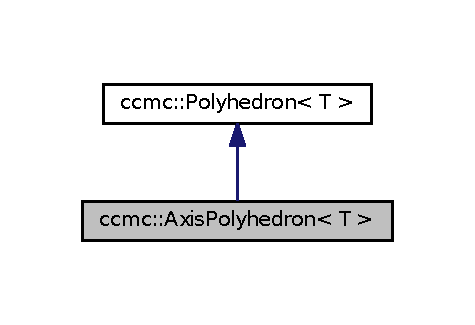
\includegraphics[width=210pt]{classccmc_1_1_axis_polyhedron__inherit__graph}
\end{center}
\end{figure}


Collaboration diagram for ccmc\-:\-:Axis\-Polyhedron$<$ T $>$\-:\nopagebreak
\begin{figure}[H]
\begin{center}
\leavevmode
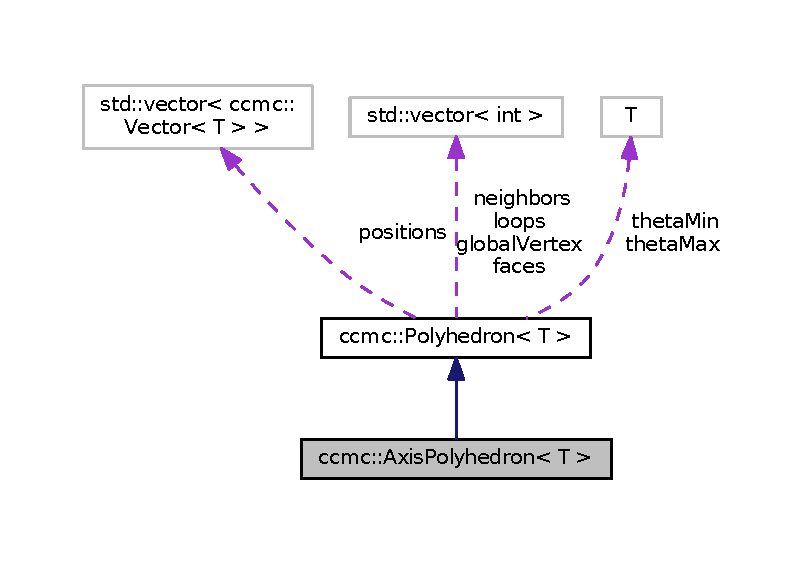
\includegraphics[width=345pt]{classccmc_1_1_axis_polyhedron__coll__graph}
\end{center}
\end{figure}
\subsection*{Public Member Functions}
\begin{DoxyCompactItemize}
\item 
\hyperlink{classccmc_1_1_axis_polyhedron_a8a2b01ae4d6a18e7813af1fea4ac1c10}{Axis\-Polyhedron} (int a, bool dday, \hyperlink{classccmc_1_1_l_f_m_interpolator}{ccmc\-::\-L\-F\-M\-Interpolator} $\ast$lfm)
\item 
int \hyperlink{classccmc_1_1_axis_polyhedron_a03d10924c8c45085ba984bb7d669bcce}{get\-Type} ()
\end{DoxyCompactItemize}
\subsection*{Public Attributes}
\begin{DoxyCompactItemize}
\item 
int \hyperlink{classccmc_1_1_axis_polyhedron_a86bf3b4fab1d62d902ecbc97b1ff2b7f}{poly\-I}
\item 
bool \hyperlink{classccmc_1_1_axis_polyhedron_a1f981cc1441ff15a0e5a80f666b3bcbb}{day}
\item 
int \hyperlink{classccmc_1_1_axis_polyhedron_ac3160e03e3b37a3ca3eb2022662f7bd2}{ni}
\item 
int \hyperlink{classccmc_1_1_axis_polyhedron_a62de873c6e6bd244a75fe64a2538f501}{nj}
\item 
int \hyperlink{classccmc_1_1_axis_polyhedron_a9fb6852015288390760e0e231daef379}{nk}
\end{DoxyCompactItemize}
\subsection*{Additional Inherited Members}


\subsection{Constructor \& Destructor Documentation}
\hypertarget{classccmc_1_1_axis_polyhedron_a8a2b01ae4d6a18e7813af1fea4ac1c10}{\index{ccmc\-::\-Axis\-Polyhedron@{ccmc\-::\-Axis\-Polyhedron}!Axis\-Polyhedron@{Axis\-Polyhedron}}
\index{Axis\-Polyhedron@{Axis\-Polyhedron}!ccmc::AxisPolyhedron@{ccmc\-::\-Axis\-Polyhedron}}
\subsubsection[{Axis\-Polyhedron}]{\setlength{\rightskip}{0pt plus 5cm}template$<$class T $>$ {\bf ccmc\-::\-Axis\-Polyhedron}$<$ T $>$\-::{\bf Axis\-Polyhedron} (
\begin{DoxyParamCaption}
\item[{int}]{a, }
\item[{bool}]{dday, }
\item[{{\bf ccmc\-::\-L\-F\-M\-Interpolator} $\ast$}]{lfm}
\end{DoxyParamCaption}
)}}\label{classccmc_1_1_axis_polyhedron_a8a2b01ae4d6a18e7813af1fea4ac1c10}


Here is the call graph for this function\-:\nopagebreak
\begin{figure}[H]
\begin{center}
\leavevmode
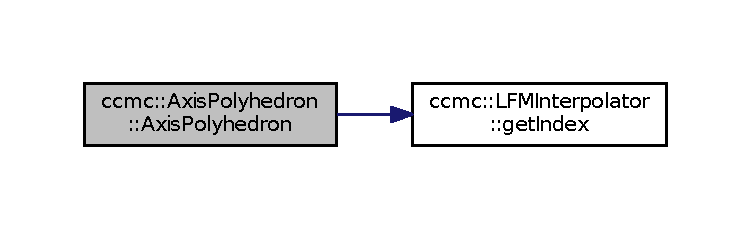
\includegraphics[width=350pt]{classccmc_1_1_axis_polyhedron_a8a2b01ae4d6a18e7813af1fea4ac1c10_cgraph}
\end{center}
\end{figure}




\subsection{Member Function Documentation}
\hypertarget{classccmc_1_1_axis_polyhedron_a03d10924c8c45085ba984bb7d669bcce}{\index{ccmc\-::\-Axis\-Polyhedron@{ccmc\-::\-Axis\-Polyhedron}!get\-Type@{get\-Type}}
\index{get\-Type@{get\-Type}!ccmc::AxisPolyhedron@{ccmc\-::\-Axis\-Polyhedron}}
\subsubsection[{get\-Type}]{\setlength{\rightskip}{0pt plus 5cm}template$<$class T $>$ int {\bf ccmc\-::\-Axis\-Polyhedron}$<$ T $>$\-::get\-Type (
\begin{DoxyParamCaption}
{}
\end{DoxyParamCaption}
)\hspace{0.3cm}{\ttfamily [virtual]}}}\label{classccmc_1_1_axis_polyhedron_a03d10924c8c45085ba984bb7d669bcce}
Returns the type of \hyperlink{classccmc_1_1_polyhedron}{Polyhedron} this is. This prototype just returns 0. 

Reimplemented from \hyperlink{classccmc_1_1_polyhedron_abef63d69bf96e4bacb000546631a048e}{ccmc\-::\-Polyhedron$<$ T $>$}.



\subsection{Member Data Documentation}
\hypertarget{classccmc_1_1_axis_polyhedron_a1f981cc1441ff15a0e5a80f666b3bcbb}{\index{ccmc\-::\-Axis\-Polyhedron@{ccmc\-::\-Axis\-Polyhedron}!day@{day}}
\index{day@{day}!ccmc::AxisPolyhedron@{ccmc\-::\-Axis\-Polyhedron}}
\subsubsection[{day}]{\setlength{\rightskip}{0pt plus 5cm}template$<$class T$>$ bool {\bf ccmc\-::\-Axis\-Polyhedron}$<$ T $>$\-::day}}\label{classccmc_1_1_axis_polyhedron_a1f981cc1441ff15a0e5a80f666b3bcbb}
\hypertarget{classccmc_1_1_axis_polyhedron_ac3160e03e3b37a3ca3eb2022662f7bd2}{\index{ccmc\-::\-Axis\-Polyhedron@{ccmc\-::\-Axis\-Polyhedron}!ni@{ni}}
\index{ni@{ni}!ccmc::AxisPolyhedron@{ccmc\-::\-Axis\-Polyhedron}}
\subsubsection[{ni}]{\setlength{\rightskip}{0pt plus 5cm}template$<$class T$>$ int {\bf ccmc\-::\-Axis\-Polyhedron}$<$ T $>$\-::ni}}\label{classccmc_1_1_axis_polyhedron_ac3160e03e3b37a3ca3eb2022662f7bd2}
\hypertarget{classccmc_1_1_axis_polyhedron_a62de873c6e6bd244a75fe64a2538f501}{\index{ccmc\-::\-Axis\-Polyhedron@{ccmc\-::\-Axis\-Polyhedron}!nj@{nj}}
\index{nj@{nj}!ccmc::AxisPolyhedron@{ccmc\-::\-Axis\-Polyhedron}}
\subsubsection[{nj}]{\setlength{\rightskip}{0pt plus 5cm}template$<$class T$>$ int {\bf ccmc\-::\-Axis\-Polyhedron}$<$ T $>$\-::nj}}\label{classccmc_1_1_axis_polyhedron_a62de873c6e6bd244a75fe64a2538f501}
\hypertarget{classccmc_1_1_axis_polyhedron_a9fb6852015288390760e0e231daef379}{\index{ccmc\-::\-Axis\-Polyhedron@{ccmc\-::\-Axis\-Polyhedron}!nk@{nk}}
\index{nk@{nk}!ccmc::AxisPolyhedron@{ccmc\-::\-Axis\-Polyhedron}}
\subsubsection[{nk}]{\setlength{\rightskip}{0pt plus 5cm}template$<$class T$>$ int {\bf ccmc\-::\-Axis\-Polyhedron}$<$ T $>$\-::nk}}\label{classccmc_1_1_axis_polyhedron_a9fb6852015288390760e0e231daef379}
\hypertarget{classccmc_1_1_axis_polyhedron_a86bf3b4fab1d62d902ecbc97b1ff2b7f}{\index{ccmc\-::\-Axis\-Polyhedron@{ccmc\-::\-Axis\-Polyhedron}!poly\-I@{poly\-I}}
\index{poly\-I@{poly\-I}!ccmc::AxisPolyhedron@{ccmc\-::\-Axis\-Polyhedron}}
\subsubsection[{poly\-I}]{\setlength{\rightskip}{0pt plus 5cm}template$<$class T$>$ int {\bf ccmc\-::\-Axis\-Polyhedron}$<$ T $>$\-::poly\-I}}\label{classccmc_1_1_axis_polyhedron_a86bf3b4fab1d62d902ecbc97b1ff2b7f}


The documentation for this class was generated from the following file\-:\begin{DoxyCompactItemize}
\item 
/\-Users/apembrok/git/ccmc-\/software/kameleon-\/plus/trunk/kameleon-\/plus-\/working/src/ccmc/\hyperlink{_l_f_m_interpolator_8h}{L\-F\-M\-Interpolator.\-h}\end{DoxyCompactItemize}

\hypertarget{classccmc_1_1_b_a_t_s_r_u_s}{\section{ccmc\-:\-:B\-A\-T\-S\-R\-U\-S Class Reference}
\label{classccmc_1_1_b_a_t_s_r_u_s}\index{ccmc\-::\-B\-A\-T\-S\-R\-U\-S@{ccmc\-::\-B\-A\-T\-S\-R\-U\-S}}
}


T\-O\-D\-O\-: brief description of \hyperlink{classccmc_1_1_b_a_t_s_r_u_s}{B\-A\-T\-S\-R\-U\-S} class.  




{\ttfamily \#include $<$ccmc/\-B\-A\-T\-S\-R\-U\-S.\-h$>$}



Inheritance diagram for ccmc\-:\-:B\-A\-T\-S\-R\-U\-S\-:
\nopagebreak
\begin{figure}[H]
\begin{center}
\leavevmode
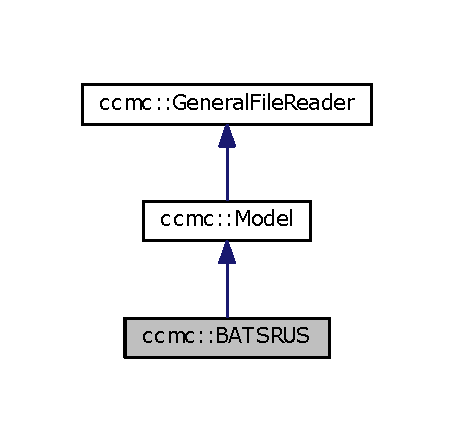
\includegraphics[width=212pt]{classccmc_1_1_b_a_t_s_r_u_s__inherit__graph}
\end{center}
\end{figure}


Collaboration diagram for ccmc\-:\-:B\-A\-T\-S\-R\-U\-S\-:
\nopagebreak
\begin{figure}[H]
\begin{center}
\leavevmode
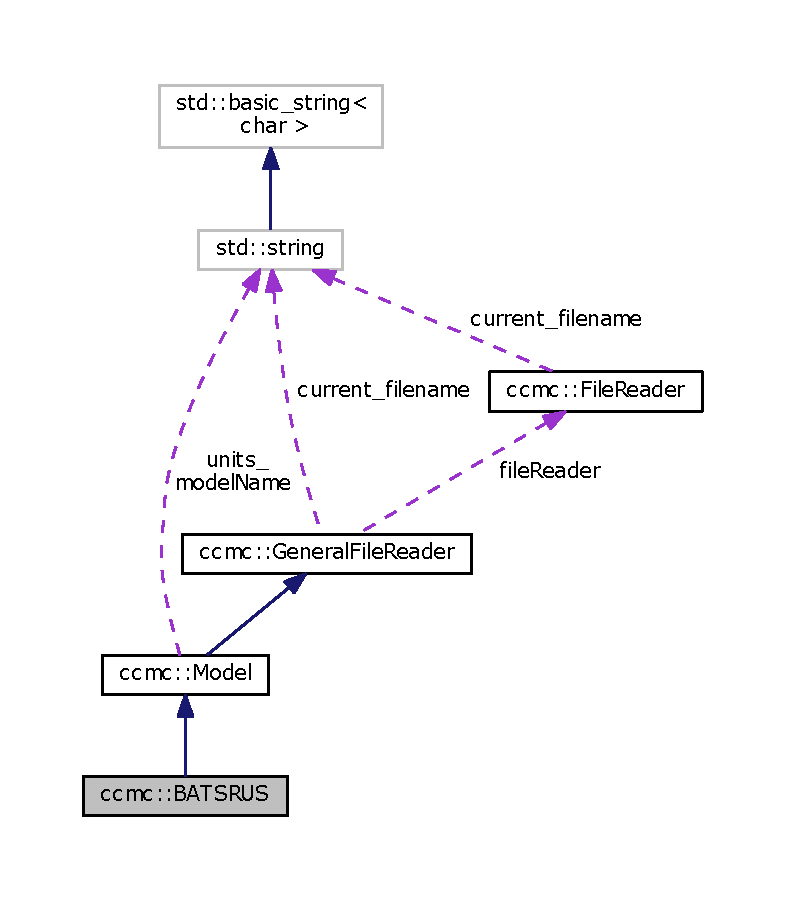
\includegraphics[width=350pt]{classccmc_1_1_b_a_t_s_r_u_s__coll__graph}
\end{center}
\end{figure}
\subsection*{Public Member Functions}
\begin{DoxyCompactItemize}
\item 
\hyperlink{classccmc_1_1_b_a_t_s_r_u_s_a687bb4cafb036eb5149d5d52be52037d}{B\-A\-T\-S\-R\-U\-S} ()
\item 
long \hyperlink{classccmc_1_1_b_a_t_s_r_u_s_a9acf9929698159533b7a50734665dd1a}{open} (const std\-::string \&filename)
\begin{DoxyCompactList}\small\item\em Opens a file.  \end{DoxyCompactList}\item 
\hyperlink{classccmc_1_1_interpolator}{Interpolator} $\ast$ \hyperlink{classccmc_1_1_b_a_t_s_r_u_s_a3cbd68c8c3fb850c3b10cb314c0a21b3}{create\-New\-Interpolator} ()
\begin{DoxyCompactList}\small\item\em Returns an \hyperlink{classccmc_1_1_interpolator}{Interpolator} object for the currently opened file.  \end{DoxyCompactList}\item 
virtual \hyperlink{classccmc_1_1_b_a_t_s_r_u_s_a087125c4f1ee6883206fd63bf8fb1528}{$\sim$\-B\-A\-T\-S\-R\-U\-S} ()
\end{DoxyCompactItemize}
\subsection*{Protected Member Functions}
\begin{DoxyCompactItemize}
\item 
void \hyperlink{classccmc_1_1_b_a_t_s_r_u_s_a86dddd02ea3db46068f482d59f77df86}{initialize\-Conversion\-Factors\-To\-S\-I} ()
\begin{DoxyCompactList}\small\item\em Initializes the conversion\-Factors\-To\-S\-I map.  \end{DoxyCompactList}\item 
void \hyperlink{classccmc_1_1_b_a_t_s_r_u_s_ab86a0088002795bbf4b60fd89576604e}{initialize\-S\-I\-Units} ()
\begin{DoxyCompactList}\small\item\em Initializes the variable\-S\-I\-Units map.  \end{DoxyCompactList}\end{DoxyCompactItemize}
\subsection*{Friends}
\begin{DoxyCompactItemize}
\item 
{\footnotesize template$<$typename T $>$ }\\int \hyperlink{classccmc_1_1_b_a_t_s_r_u_s_ae33f5d913530545859c1b8b43200c237}{binary\-\_\-search} (const std\-::vector$<$ T $>$ \&vec, unsigned int start, unsigned int end, const T \&key)
\end{DoxyCompactItemize}
\subsection*{Additional Inherited Members}


\subsection{Detailed Description}
T\-O\-D\-O\-: brief description of \hyperlink{classccmc_1_1_b_a_t_s_r_u_s}{B\-A\-T\-S\-R\-U\-S} class. 

T\-O\-D\-O\-: full description of \hyperlink{classccmc_1_1_b_a_t_s_r_u_s}{B\-A\-T\-S\-R\-U\-S} class 

\subsection{Constructor \& Destructor Documentation}
\hypertarget{classccmc_1_1_b_a_t_s_r_u_s_a687bb4cafb036eb5149d5d52be52037d}{\index{ccmc\-::\-B\-A\-T\-S\-R\-U\-S@{ccmc\-::\-B\-A\-T\-S\-R\-U\-S}!B\-A\-T\-S\-R\-U\-S@{B\-A\-T\-S\-R\-U\-S}}
\index{B\-A\-T\-S\-R\-U\-S@{B\-A\-T\-S\-R\-U\-S}!ccmc::BATSRUS@{ccmc\-::\-B\-A\-T\-S\-R\-U\-S}}
\subsubsection[{B\-A\-T\-S\-R\-U\-S}]{\setlength{\rightskip}{0pt plus 5cm}ccmc\-::\-B\-A\-T\-S\-R\-U\-S\-::\-B\-A\-T\-S\-R\-U\-S (
\begin{DoxyParamCaption}
{}
\end{DoxyParamCaption}
)}}\label{classccmc_1_1_b_a_t_s_r_u_s_a687bb4cafb036eb5149d5d52be52037d}
Default constructor \hypertarget{classccmc_1_1_b_a_t_s_r_u_s_a087125c4f1ee6883206fd63bf8fb1528}{\index{ccmc\-::\-B\-A\-T\-S\-R\-U\-S@{ccmc\-::\-B\-A\-T\-S\-R\-U\-S}!$\sim$\-B\-A\-T\-S\-R\-U\-S@{$\sim$\-B\-A\-T\-S\-R\-U\-S}}
\index{$\sim$\-B\-A\-T\-S\-R\-U\-S@{$\sim$\-B\-A\-T\-S\-R\-U\-S}!ccmc::BATSRUS@{ccmc\-::\-B\-A\-T\-S\-R\-U\-S}}
\subsubsection[{$\sim$\-B\-A\-T\-S\-R\-U\-S}]{\setlength{\rightskip}{0pt plus 5cm}ccmc\-::\-B\-A\-T\-S\-R\-U\-S\-::$\sim$\-B\-A\-T\-S\-R\-U\-S (
\begin{DoxyParamCaption}
{}
\end{DoxyParamCaption}
)\hspace{0.3cm}{\ttfamily [virtual]}}}\label{classccmc_1_1_b_a_t_s_r_u_s_a087125c4f1ee6883206fd63bf8fb1528}
Destructor 

\subsection{Member Function Documentation}
\hypertarget{classccmc_1_1_b_a_t_s_r_u_s_a3cbd68c8c3fb850c3b10cb314c0a21b3}{\index{ccmc\-::\-B\-A\-T\-S\-R\-U\-S@{ccmc\-::\-B\-A\-T\-S\-R\-U\-S}!create\-New\-Interpolator@{create\-New\-Interpolator}}
\index{create\-New\-Interpolator@{create\-New\-Interpolator}!ccmc::BATSRUS@{ccmc\-::\-B\-A\-T\-S\-R\-U\-S}}
\subsubsection[{create\-New\-Interpolator}]{\setlength{\rightskip}{0pt plus 5cm}{\bf Interpolator} $\ast$ ccmc\-::\-B\-A\-T\-S\-R\-U\-S\-::create\-New\-Interpolator (
\begin{DoxyParamCaption}
{}
\end{DoxyParamCaption}
)\hspace{0.3cm}{\ttfamily [virtual]}}}\label{classccmc_1_1_b_a_t_s_r_u_s_a3cbd68c8c3fb850c3b10cb314c0a21b3}


Returns an \hyperlink{classccmc_1_1_interpolator}{Interpolator} object for the currently opened file.  

This returns an \hyperlink{classccmc_1_1_interpolator}{Interpolator} object that contains all the necessary local variables required to interpolate independent of any other \hyperlink{classccmc_1_1_interpolator}{Interpolator} object. The pointer must be deleted from the calling program. \begin{DoxyReturn}{Returns}
A pointer to an \hyperlink{classccmc_1_1_interpolator}{Interpolator} object. 
\end{DoxyReturn}
 

Implements \hyperlink{classccmc_1_1_model_a0dd491507c14502c27aa61b020fca8cc}{ccmc\-::\-Model}.

\hypertarget{classccmc_1_1_b_a_t_s_r_u_s_a86dddd02ea3db46068f482d59f77df86}{\index{ccmc\-::\-B\-A\-T\-S\-R\-U\-S@{ccmc\-::\-B\-A\-T\-S\-R\-U\-S}!initialize\-Conversion\-Factors\-To\-S\-I@{initialize\-Conversion\-Factors\-To\-S\-I}}
\index{initialize\-Conversion\-Factors\-To\-S\-I@{initialize\-Conversion\-Factors\-To\-S\-I}!ccmc::BATSRUS@{ccmc\-::\-B\-A\-T\-S\-R\-U\-S}}
\subsubsection[{initialize\-Conversion\-Factors\-To\-S\-I}]{\setlength{\rightskip}{0pt plus 5cm}void ccmc\-::\-B\-A\-T\-S\-R\-U\-S\-::initialize\-Conversion\-Factors\-To\-S\-I (
\begin{DoxyParamCaption}
{}
\end{DoxyParamCaption}
)\hspace{0.3cm}{\ttfamily [protected]}, {\ttfamily [virtual]}}}\label{classccmc_1_1_b_a_t_s_r_u_s_a86dddd02ea3db46068f482d59f77df86}


Initializes the conversion\-Factors\-To\-S\-I map.  

These factors are used to convert interpolated values to S\-I units.  T\-O\-D\-O\-: fix these conversion factors

Implements \hyperlink{classccmc_1_1_model_a6f04326691fba448e2cfb7c7ab90a45a}{ccmc\-::\-Model}.

\hypertarget{classccmc_1_1_b_a_t_s_r_u_s_ab86a0088002795bbf4b60fd89576604e}{\index{ccmc\-::\-B\-A\-T\-S\-R\-U\-S@{ccmc\-::\-B\-A\-T\-S\-R\-U\-S}!initialize\-S\-I\-Units@{initialize\-S\-I\-Units}}
\index{initialize\-S\-I\-Units@{initialize\-S\-I\-Units}!ccmc::BATSRUS@{ccmc\-::\-B\-A\-T\-S\-R\-U\-S}}
\subsubsection[{initialize\-S\-I\-Units}]{\setlength{\rightskip}{0pt plus 5cm}void ccmc\-::\-B\-A\-T\-S\-R\-U\-S\-::initialize\-S\-I\-Units (
\begin{DoxyParamCaption}
{}
\end{DoxyParamCaption}
)\hspace{0.3cm}{\ttfamily [protected]}, {\ttfamily [virtual]}}}\label{classccmc_1_1_b_a_t_s_r_u_s_ab86a0088002795bbf4b60fd89576604e}


Initializes the variable\-S\-I\-Units map.  



Implements \hyperlink{classccmc_1_1_model_a68d31e8d8cce59269c994de25d048178}{ccmc\-::\-Model}.

\hypertarget{classccmc_1_1_b_a_t_s_r_u_s_a9acf9929698159533b7a50734665dd1a}{\index{ccmc\-::\-B\-A\-T\-S\-R\-U\-S@{ccmc\-::\-B\-A\-T\-S\-R\-U\-S}!open@{open}}
\index{open@{open}!ccmc::BATSRUS@{ccmc\-::\-B\-A\-T\-S\-R\-U\-S}}
\subsubsection[{open}]{\setlength{\rightskip}{0pt plus 5cm}long ccmc\-::\-B\-A\-T\-S\-R\-U\-S\-::open (
\begin{DoxyParamCaption}
\item[{const std\-::string \&}]{filename}
\end{DoxyParamCaption}
)\hspace{0.3cm}{\ttfamily [virtual]}}}\label{classccmc_1_1_b_a_t_s_r_u_s_a9acf9929698159533b7a50734665dd1a}


Opens a file.  

Opens a file and performs any necessary initialization required to work with the data. 
\begin{DoxyParams}{Parameters}
{\em filename} & \\
\hline
\end{DoxyParams}
 

Implements \hyperlink{classccmc_1_1_model_a3c64dc635c2c1a2fe2f8efa2a3666282}{ccmc\-::\-Model}.



Here is the call graph for this function\-:
\nopagebreak
\begin{figure}[H]
\begin{center}
\leavevmode
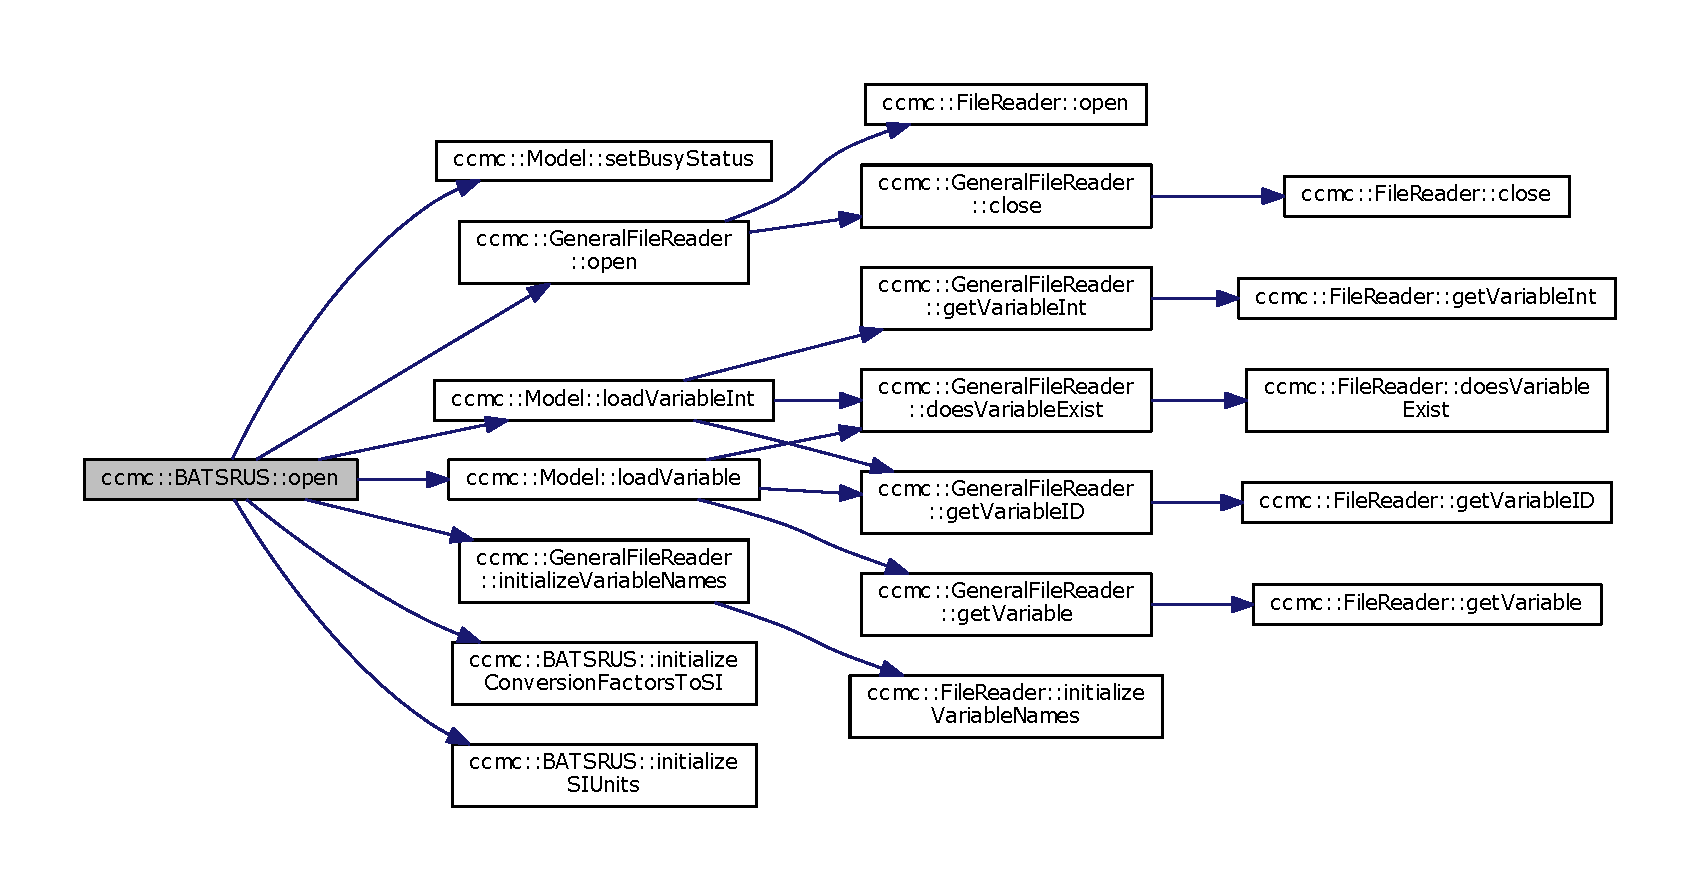
\includegraphics[width=350pt]{classccmc_1_1_b_a_t_s_r_u_s_a9acf9929698159533b7a50734665dd1a_cgraph}
\end{center}
\end{figure}




\subsection{Friends And Related Function Documentation}
\hypertarget{classccmc_1_1_b_a_t_s_r_u_s_ae33f5d913530545859c1b8b43200c237}{\index{ccmc\-::\-B\-A\-T\-S\-R\-U\-S@{ccmc\-::\-B\-A\-T\-S\-R\-U\-S}!binary\-\_\-search@{binary\-\_\-search}}
\index{binary\-\_\-search@{binary\-\_\-search}!ccmc::BATSRUS@{ccmc\-::\-B\-A\-T\-S\-R\-U\-S}}
\subsubsection[{binary\-\_\-search}]{\setlength{\rightskip}{0pt plus 5cm}template$<$typename T $>$ int binary\-\_\-search (
\begin{DoxyParamCaption}
\item[{const std\-::vector$<$ T $>$ \&}]{vec, }
\item[{unsigned int}]{start, }
\item[{unsigned int}]{end, }
\item[{const T \&}]{key}
\end{DoxyParamCaption}
)\hspace{0.3cm}{\ttfamily [friend]}}}\label{classccmc_1_1_b_a_t_s_r_u_s_ae33f5d913530545859c1b8b43200c237}


The documentation for this class was generated from the following files\-:\begin{DoxyCompactItemize}
\item 
/\-Users/dberrios/\-Documents/workspace/kameleon-\/plus/src/ccmc/\hyperlink{_b_a_t_s_r_u_s_8h}{B\-A\-T\-S\-R\-U\-S.\-h}\item 
/\-Users/dberrios/\-Documents/workspace/kameleon-\/plus/src/ccmc/\hyperlink{_b_a_t_s_r_u_s_8cpp}{B\-A\-T\-S\-R\-U\-S.\-cpp}\end{DoxyCompactItemize}

\hypertarget{classccmc_1_1_b_a_t_s_r_u_s_interpolator}{\section{ccmc\-:\-:B\-A\-T\-S\-R\-U\-S\-Interpolator Class Reference}
\label{classccmc_1_1_b_a_t_s_r_u_s_interpolator}\index{ccmc\-::\-B\-A\-T\-S\-R\-U\-S\-Interpolator@{ccmc\-::\-B\-A\-T\-S\-R\-U\-S\-Interpolator}}
}


T\-O\-D\-O\-: brief description of \hyperlink{classccmc_1_1_b_a_t_s_r_u_s_interpolator}{B\-A\-T\-S\-R\-U\-S\-Interpolator} class.  




{\ttfamily \#include $<$B\-A\-T\-S\-R\-U\-S\-Interpolator.\-h$>$}



Inheritance diagram for ccmc\-:\-:B\-A\-T\-S\-R\-U\-S\-Interpolator\-:\nopagebreak
\begin{figure}[H]
\begin{center}
\leavevmode
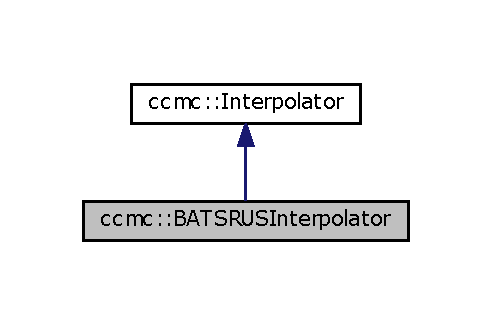
\includegraphics[width=236pt]{classccmc_1_1_b_a_t_s_r_u_s_interpolator__inherit__graph}
\end{center}
\end{figure}


Collaboration diagram for ccmc\-:\-:B\-A\-T\-S\-R\-U\-S\-Interpolator\-:\nopagebreak
\begin{figure}[H]
\begin{center}
\leavevmode
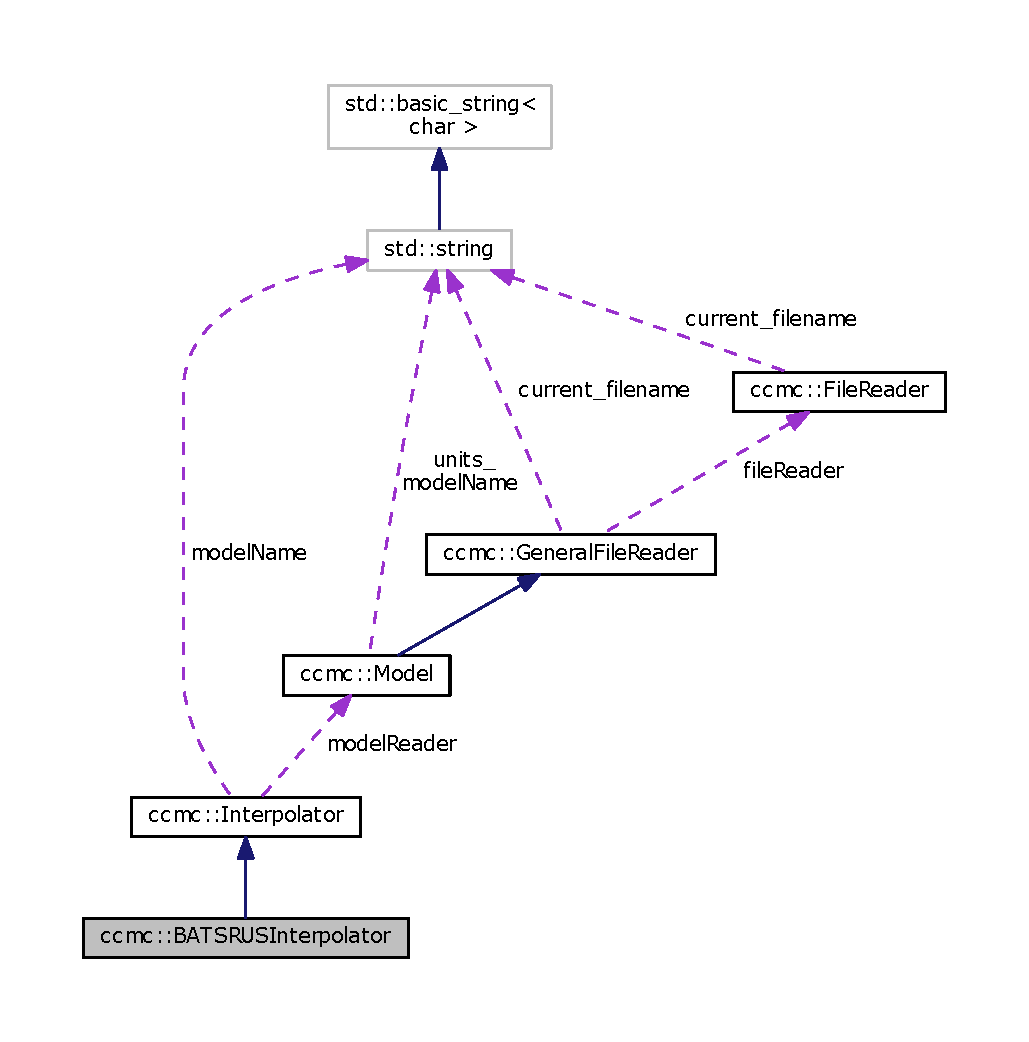
\includegraphics[width=350pt]{classccmc_1_1_b_a_t_s_r_u_s_interpolator__coll__graph}
\end{center}
\end{figure}
\subsection*{Public Member Functions}
\begin{DoxyCompactItemize}
\item 
\hyperlink{classccmc_1_1_b_a_t_s_r_u_s_interpolator_a13070c4466906bd409bb948bc378b64c}{B\-A\-T\-S\-R\-U\-S\-Interpolator} (\hyperlink{classccmc_1_1_model}{Model} $\ast$\hyperlink{classccmc_1_1_interpolator_afee5bb61e5d5a0a7b9152c6f74378c4a}{model\-Reader})
\item 
float \hyperlink{classccmc_1_1_b_a_t_s_r_u_s_interpolator_a9a9a185e83767d1bfc9b1bb584cd250f}{interpolate} (const std\-::string \&, const float \&c0, const float \&c1, const float \&c2)
\item 
float \hyperlink{classccmc_1_1_b_a_t_s_r_u_s_interpolator_ab5e4f01a95ee9b9d1a58868806d8fa42}{interpolate} (const std\-::string \&, const float \&c0, const float \&c1, const float \&c2, float \&dc0, float \&dc1, float \&dc2)
\item 
float \hyperlink{classccmc_1_1_b_a_t_s_r_u_s_interpolator_ae6577b5c388106e6d26f1c890a30cba8}{interpolate} (const long \&variable\-\_\-id, const float \&c0, const float \&c1, const float \&c2)
\item 
float \hyperlink{classccmc_1_1_b_a_t_s_r_u_s_interpolator_a8bb4e9b10064a516192c771462673b09}{interpolate} (const long \&variable\-\_\-id, const float \&c0, const float \&c1, const float \&c2, float \&dc0, float \&dc1, float \&dc2)
\item 
virtual \hyperlink{classccmc_1_1_b_a_t_s_r_u_s_interpolator_a5c188e0bf30c66f3aadc34d1c2711937}{$\sim$\-B\-A\-T\-S\-R\-U\-S\-Interpolator} ()
\end{DoxyCompactItemize}
\subsection*{Additional Inherited Members}


\subsection{Detailed Description}
T\-O\-D\-O\-: brief description of \hyperlink{classccmc_1_1_b_a_t_s_r_u_s_interpolator}{B\-A\-T\-S\-R\-U\-S\-Interpolator} class. 

T\-O\-D\-O\-: full description of \hyperlink{classccmc_1_1_b_a_t_s_r_u_s_interpolator}{B\-A\-T\-S\-R\-U\-S\-Interpolator} class 

\subsection{Constructor \& Destructor Documentation}
\hypertarget{classccmc_1_1_b_a_t_s_r_u_s_interpolator_a13070c4466906bd409bb948bc378b64c}{\index{ccmc\-::\-B\-A\-T\-S\-R\-U\-S\-Interpolator@{ccmc\-::\-B\-A\-T\-S\-R\-U\-S\-Interpolator}!B\-A\-T\-S\-R\-U\-S\-Interpolator@{B\-A\-T\-S\-R\-U\-S\-Interpolator}}
\index{B\-A\-T\-S\-R\-U\-S\-Interpolator@{B\-A\-T\-S\-R\-U\-S\-Interpolator}!ccmc::BATSRUSInterpolator@{ccmc\-::\-B\-A\-T\-S\-R\-U\-S\-Interpolator}}
\subsubsection[{B\-A\-T\-S\-R\-U\-S\-Interpolator}]{\setlength{\rightskip}{0pt plus 5cm}ccmc\-::\-B\-A\-T\-S\-R\-U\-S\-Interpolator\-::\-B\-A\-T\-S\-R\-U\-S\-Interpolator (
\begin{DoxyParamCaption}
\item[{{\bf Model} $\ast$}]{model\-Reader}
\end{DoxyParamCaption}
)}}\label{classccmc_1_1_b_a_t_s_r_u_s_interpolator_a13070c4466906bd409bb948bc378b64c}

\begin{DoxyParams}{Parameters}
{\em model\-Reader} & Pointer to the \hyperlink{classccmc_1_1_model}{Model} object containing the appropriate variable maps. \hyperlink{classccmc_1_1_b_a_t_s_r_u_s_interpolator}{B\-A\-T\-S\-R\-U\-S\-Interpolator} should be returned by a \hyperlink{classccmc_1_1_b_a_t_s_r_u_s_a3cbd68c8c3fb850c3b10cb314c0a21b3}{B\-A\-T\-S\-R\-U\-S\-::create\-New\-Interpolator()} call. \\
\hline
\end{DoxyParams}
They are stored as floats. Need to fetch them, and convert to int 

Here is the call graph for this function\-:\nopagebreak
\begin{figure}[H]
\begin{center}
\leavevmode
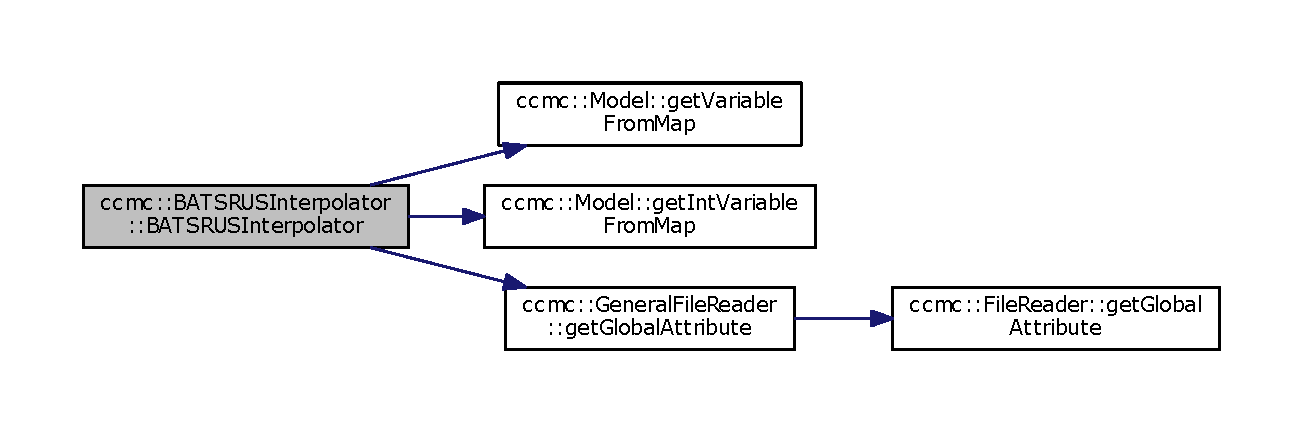
\includegraphics[width=350pt]{classccmc_1_1_b_a_t_s_r_u_s_interpolator_a13070c4466906bd409bb948bc378b64c_cgraph}
\end{center}
\end{figure}


\hypertarget{classccmc_1_1_b_a_t_s_r_u_s_interpolator_a5c188e0bf30c66f3aadc34d1c2711937}{\index{ccmc\-::\-B\-A\-T\-S\-R\-U\-S\-Interpolator@{ccmc\-::\-B\-A\-T\-S\-R\-U\-S\-Interpolator}!$\sim$\-B\-A\-T\-S\-R\-U\-S\-Interpolator@{$\sim$\-B\-A\-T\-S\-R\-U\-S\-Interpolator}}
\index{$\sim$\-B\-A\-T\-S\-R\-U\-S\-Interpolator@{$\sim$\-B\-A\-T\-S\-R\-U\-S\-Interpolator}!ccmc::BATSRUSInterpolator@{ccmc\-::\-B\-A\-T\-S\-R\-U\-S\-Interpolator}}
\subsubsection[{$\sim$\-B\-A\-T\-S\-R\-U\-S\-Interpolator}]{\setlength{\rightskip}{0pt plus 5cm}ccmc\-::\-B\-A\-T\-S\-R\-U\-S\-Interpolator\-::$\sim$\-B\-A\-T\-S\-R\-U\-S\-Interpolator (
\begin{DoxyParamCaption}
{}
\end{DoxyParamCaption}
)\hspace{0.3cm}{\ttfamily [virtual]}}}\label{classccmc_1_1_b_a_t_s_r_u_s_interpolator_a5c188e0bf30c66f3aadc34d1c2711937}
Destructor 

\subsection{Member Function Documentation}
\hypertarget{classccmc_1_1_b_a_t_s_r_u_s_interpolator_a9a9a185e83767d1bfc9b1bb584cd250f}{\index{ccmc\-::\-B\-A\-T\-S\-R\-U\-S\-Interpolator@{ccmc\-::\-B\-A\-T\-S\-R\-U\-S\-Interpolator}!interpolate@{interpolate}}
\index{interpolate@{interpolate}!ccmc::BATSRUSInterpolator@{ccmc\-::\-B\-A\-T\-S\-R\-U\-S\-Interpolator}}
\subsubsection[{interpolate}]{\setlength{\rightskip}{0pt plus 5cm}float ccmc\-::\-B\-A\-T\-S\-R\-U\-S\-Interpolator\-::interpolate (
\begin{DoxyParamCaption}
\item[{const std\-::string \&}]{variable, }
\item[{const float \&}]{c0, }
\item[{const float \&}]{c1, }
\item[{const float \&}]{c2}
\end{DoxyParamCaption}
)\hspace{0.3cm}{\ttfamily [virtual]}}}\label{classccmc_1_1_b_a_t_s_r_u_s_interpolator_a9a9a185e83767d1bfc9b1bb584cd250f}

\begin{DoxyParams}{Parameters}
{\em variable} & \\
\hline
{\em c0} & X component of the position \\
\hline
{\em c1} & Y component of the position \\
\hline
{\em c2} & Z component of the position \\
\hline
\end{DoxyParams}
\begin{DoxyReturn}{Returns}

\end{DoxyReturn}


Implements \hyperlink{classccmc_1_1_interpolator_ad5c1dd3693f83d75a2335b7c28cd649d}{ccmc\-::\-Interpolator}.



Here is the call graph for this function\-:\nopagebreak
\begin{figure}[H]
\begin{center}
\leavevmode
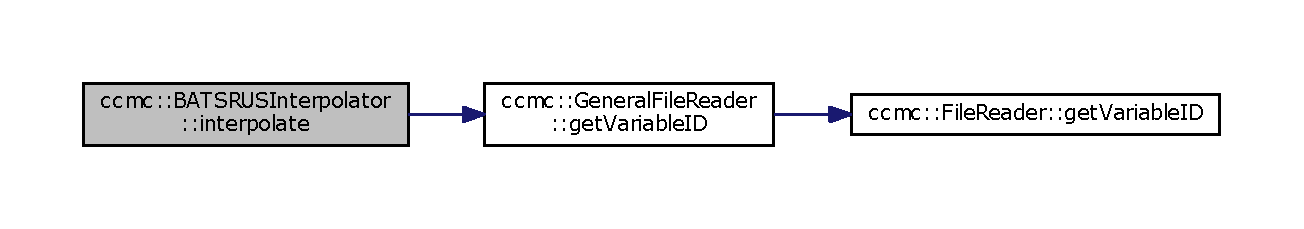
\includegraphics[width=350pt]{classccmc_1_1_b_a_t_s_r_u_s_interpolator_a9a9a185e83767d1bfc9b1bb584cd250f_cgraph}
\end{center}
\end{figure}


\hypertarget{classccmc_1_1_b_a_t_s_r_u_s_interpolator_ab5e4f01a95ee9b9d1a58868806d8fa42}{\index{ccmc\-::\-B\-A\-T\-S\-R\-U\-S\-Interpolator@{ccmc\-::\-B\-A\-T\-S\-R\-U\-S\-Interpolator}!interpolate@{interpolate}}
\index{interpolate@{interpolate}!ccmc::BATSRUSInterpolator@{ccmc\-::\-B\-A\-T\-S\-R\-U\-S\-Interpolator}}
\subsubsection[{interpolate}]{\setlength{\rightskip}{0pt plus 5cm}float ccmc\-::\-B\-A\-T\-S\-R\-U\-S\-Interpolator\-::interpolate (
\begin{DoxyParamCaption}
\item[{const std\-::string \&}]{variable, }
\item[{const float \&}]{c0, }
\item[{const float \&}]{c1, }
\item[{const float \&}]{c2, }
\item[{float \&}]{dc0, }
\item[{float \&}]{dc1, }
\item[{float \&}]{dc2}
\end{DoxyParamCaption}
)\hspace{0.3cm}{\ttfamily [virtual]}}}\label{classccmc_1_1_b_a_t_s_r_u_s_interpolator_ab5e4f01a95ee9b9d1a58868806d8fa42}
Interpolation method. Note that using the variable I\-D is significantly faster than using the variable string. 
\begin{DoxyParams}{Parameters}
{\em variable} & The input variable. \\
\hline
{\em c0} & X component of the position \\
\hline
{\em c1} & Y component of the position \\
\hline
{\em c2} & Z component of the position \\
\hline
{\em dc0} & Reference to a variable to store the delta for component 0 \\
\hline
{\em dc1} & Reference to a variable to store the delta for component 1 \\
\hline
{\em dc2} & Reference to a variable to store the delta for component 2 \\
\hline
\end{DoxyParams}
\begin{DoxyReturn}{Returns}
The interpolated value at position (c0,c1,c2) with deltas (dc0,dc1,dc2) 
\end{DoxyReturn}
end of if new position loop 

Implements \hyperlink{classccmc_1_1_interpolator_ae02453da5a1a8f472f33b2058424ddb6}{ccmc\-::\-Interpolator}.



Here is the call graph for this function\-:\nopagebreak
\begin{figure}[H]
\begin{center}
\leavevmode
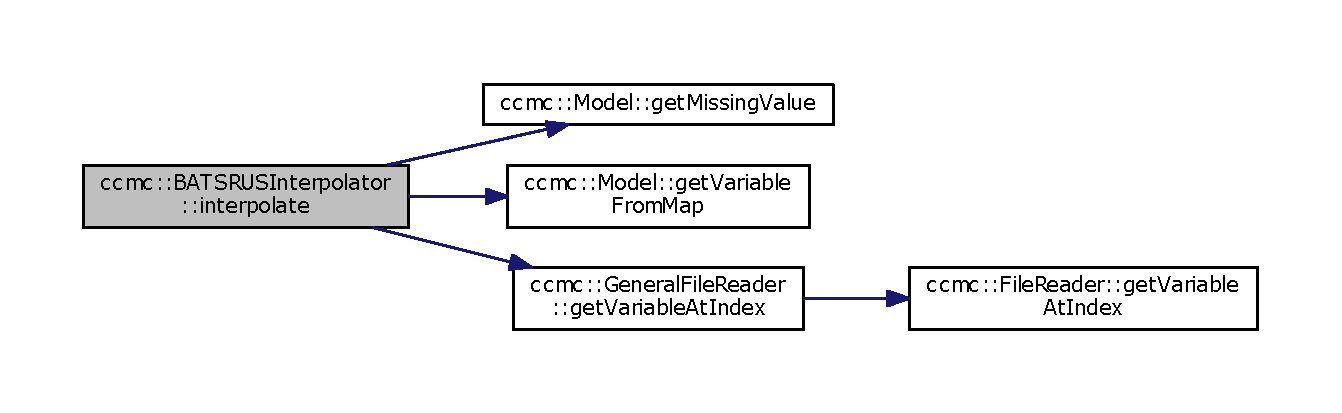
\includegraphics[width=350pt]{classccmc_1_1_b_a_t_s_r_u_s_interpolator_ab5e4f01a95ee9b9d1a58868806d8fa42_cgraph}
\end{center}
\end{figure}


\hypertarget{classccmc_1_1_b_a_t_s_r_u_s_interpolator_ae6577b5c388106e6d26f1c890a30cba8}{\index{ccmc\-::\-B\-A\-T\-S\-R\-U\-S\-Interpolator@{ccmc\-::\-B\-A\-T\-S\-R\-U\-S\-Interpolator}!interpolate@{interpolate}}
\index{interpolate@{interpolate}!ccmc::BATSRUSInterpolator@{ccmc\-::\-B\-A\-T\-S\-R\-U\-S\-Interpolator}}
\subsubsection[{interpolate}]{\setlength{\rightskip}{0pt plus 5cm}float ccmc\-::\-B\-A\-T\-S\-R\-U\-S\-Interpolator\-::interpolate (
\begin{DoxyParamCaption}
\item[{const long \&}]{variable\-\_\-id, }
\item[{const float \&}]{c0, }
\item[{const float \&}]{c1, }
\item[{const float \&}]{c2}
\end{DoxyParamCaption}
)\hspace{0.3cm}{\ttfamily [virtual]}}}\label{classccmc_1_1_b_a_t_s_r_u_s_interpolator_ae6577b5c388106e6d26f1c890a30cba8}

\begin{DoxyParams}{Parameters}
{\em variable\-\_\-id} & \\
\hline
{\em c0} & X component of the position \\
\hline
{\em c1} & Y component of the position \\
\hline
{\em c2} & Z component of the position \\
\hline
\end{DoxyParams}
\begin{DoxyReturn}{Returns}

\end{DoxyReturn}


Implements \hyperlink{classccmc_1_1_interpolator_a6bfe1b4075f03704b893bb96e1675a3b}{ccmc\-::\-Interpolator}.



Here is the call graph for this function\-:\nopagebreak
\begin{figure}[H]
\begin{center}
\leavevmode
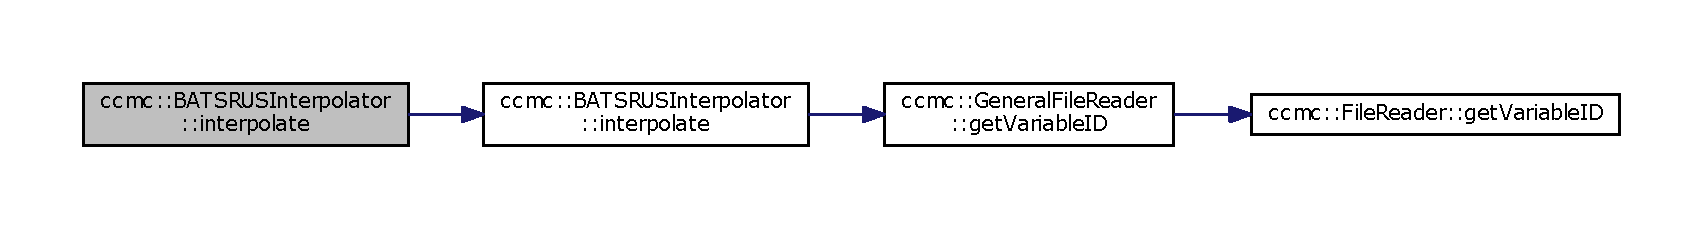
\includegraphics[width=350pt]{classccmc_1_1_b_a_t_s_r_u_s_interpolator_ae6577b5c388106e6d26f1c890a30cba8_cgraph}
\end{center}
\end{figure}


\hypertarget{classccmc_1_1_b_a_t_s_r_u_s_interpolator_a8bb4e9b10064a516192c771462673b09}{\index{ccmc\-::\-B\-A\-T\-S\-R\-U\-S\-Interpolator@{ccmc\-::\-B\-A\-T\-S\-R\-U\-S\-Interpolator}!interpolate@{interpolate}}
\index{interpolate@{interpolate}!ccmc::BATSRUSInterpolator@{ccmc\-::\-B\-A\-T\-S\-R\-U\-S\-Interpolator}}
\subsubsection[{interpolate}]{\setlength{\rightskip}{0pt plus 5cm}float ccmc\-::\-B\-A\-T\-S\-R\-U\-S\-Interpolator\-::interpolate (
\begin{DoxyParamCaption}
\item[{const long \&}]{variable\-\_\-id, }
\item[{const float \&}]{c0, }
\item[{const float \&}]{c1, }
\item[{const float \&}]{c2, }
\item[{float \&}]{dc0, }
\item[{float \&}]{dc1, }
\item[{float \&}]{dc2}
\end{DoxyParamCaption}
)\hspace{0.3cm}{\ttfamily [virtual]}}}\label{classccmc_1_1_b_a_t_s_r_u_s_interpolator_a8bb4e9b10064a516192c771462673b09}
Interpolation method. Note that using the variable I\-D is significantly faster than using the variable string. 
\begin{DoxyParams}{Parameters}
{\em variable\-\_\-id} & A long representing the variable I\-D. \\
\hline
{\em c0} & X component of the position \\
\hline
{\em c1} & Y component of the position \\
\hline
{\em c2} & Z component of the position \\
\hline
{\em dc0} & Reference to a variable to store the delta for component 0 \\
\hline
{\em dc1} & Reference to a variable to store the delta for component 1 \\
\hline
{\em dc2} & Reference to a variable to store the delta for component 2 \\
\hline
\end{DoxyParams}
\begin{DoxyReturn}{Returns}
The interpolated value at position (c0,c1,c2) with deltas (dc0,dc1,dc2) 
\end{DoxyReturn}
end of if new position loop 

Implements \hyperlink{classccmc_1_1_interpolator_aa6b272bd53630020d92938ec1e5cfad9}{ccmc\-::\-Interpolator}.



Here is the call graph for this function\-:\nopagebreak
\begin{figure}[H]
\begin{center}
\leavevmode
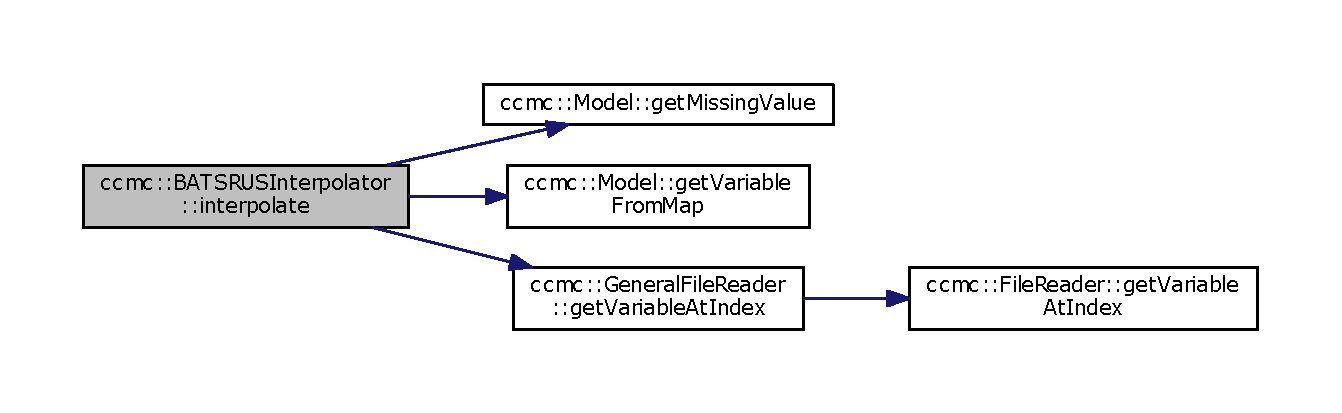
\includegraphics[width=350pt]{classccmc_1_1_b_a_t_s_r_u_s_interpolator_a8bb4e9b10064a516192c771462673b09_cgraph}
\end{center}
\end{figure}




The documentation for this class was generated from the following files\-:\begin{DoxyCompactItemize}
\item 
/\-Users/apembrok/git/ccmc-\/software/kameleon-\/plus/trunk/kameleon-\/plus-\/working/src/ccmc/\hyperlink{_b_a_t_s_r_u_s_interpolator_8h}{B\-A\-T\-S\-R\-U\-S\-Interpolator.\-h}\item 
/\-Users/apembrok/git/ccmc-\/software/kameleon-\/plus/trunk/kameleon-\/plus-\/working/src/ccmc/\hyperlink{_b_a_t_s_r_u_s_interpolator_8cpp}{B\-A\-T\-S\-R\-U\-S\-Interpolator.\-cpp}\end{DoxyCompactItemize}

\hypertarget{structnanoflann_1_1_k_d_tree_single_index_adaptor_1_1_branch_struct}{\section{nanoflann\-:\-:K\-D\-Tree\-Single\-Index\-Adaptor$<$ Distance, Dataset\-Adaptor, D\-I\-M, Index\-Type $>$\-:\-:Branch\-Struct$<$ T, Distance\-Type $>$ Struct Template Reference}
\label{structnanoflann_1_1_k_d_tree_single_index_adaptor_1_1_branch_struct}\index{nanoflann\-::\-K\-D\-Tree\-Single\-Index\-Adaptor$<$ Distance, Dataset\-Adaptor, D\-I\-M, Index\-Type $>$\-::\-Branch\-Struct$<$ T, Distance\-Type $>$@{nanoflann\-::\-K\-D\-Tree\-Single\-Index\-Adaptor$<$ Distance, Dataset\-Adaptor, D\-I\-M, Index\-Type $>$\-::\-Branch\-Struct$<$ T, Distance\-Type $>$}}
}


{\ttfamily \#include $<$nanoflann.\-hpp$>$}



Collaboration diagram for nanoflann\-:\-:K\-D\-Tree\-Single\-Index\-Adaptor$<$ Distance, Dataset\-Adaptor, D\-I\-M, Index\-Type $>$\-:\-:Branch\-Struct$<$ T, Distance\-Type $>$\-:\nopagebreak
\begin{figure}[H]
\begin{center}
\leavevmode
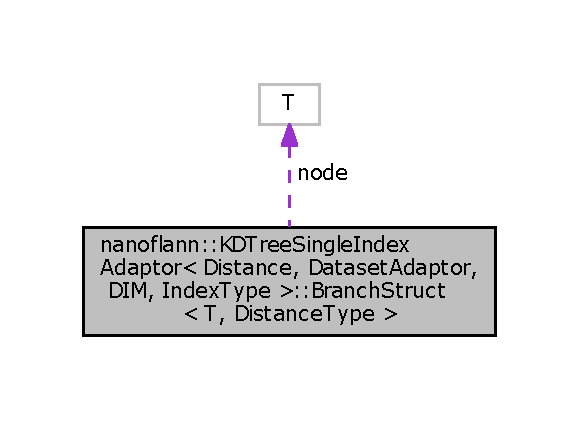
\includegraphics[width=274pt]{structnanoflann_1_1_k_d_tree_single_index_adaptor_1_1_branch_struct__coll__graph}
\end{center}
\end{figure}
\subsection*{Public Member Functions}
\begin{DoxyCompactItemize}
\item 
\hyperlink{structnanoflann_1_1_k_d_tree_single_index_adaptor_1_1_branch_struct_aba3ba55815d287de14df42bf37098ea8}{Branch\-Struct} ()
\item 
\hyperlink{structnanoflann_1_1_k_d_tree_single_index_adaptor_1_1_branch_struct_aac7996f8b84dabea451fce1460ca65fa}{Branch\-Struct} (const T \&a\-Node, \hyperlink{classnanoflann_1_1_k_d_tree_single_index_adaptor_addc764e7c19cc85c89b3903338e5a910}{Distance\-Type} dist)
\item 
bool \hyperlink{structnanoflann_1_1_k_d_tree_single_index_adaptor_1_1_branch_struct_a884cd16e926687b28daf3ce6ad520665}{operator$<$} (const \hyperlink{structnanoflann_1_1_k_d_tree_single_index_adaptor_1_1_branch_struct}{Branch\-Struct}$<$ T, \hyperlink{classnanoflann_1_1_k_d_tree_single_index_adaptor_addc764e7c19cc85c89b3903338e5a910}{Distance\-Type} $>$ \&rhs) const 
\end{DoxyCompactItemize}
\subsection*{Public Attributes}
\begin{DoxyCompactItemize}
\item 
T \hyperlink{structnanoflann_1_1_k_d_tree_single_index_adaptor_1_1_branch_struct_a86bcc74bb89be6b93db206feb8a3aad7}{node}
\item 
\hyperlink{classnanoflann_1_1_k_d_tree_single_index_adaptor_addc764e7c19cc85c89b3903338e5a910}{Distance\-Type} \hyperlink{structnanoflann_1_1_k_d_tree_single_index_adaptor_1_1_branch_struct_aa62cca16bd04ba7fd2ef25b3d3e8a6fa}{mindist}
\end{DoxyCompactItemize}


\subsection{Detailed Description}
\subsubsection*{template$<$typename Distance, class Dataset\-Adaptor, int D\-I\-M = -\/1, typename Index\-Type = size\-\_\-t$>$template$<$typename T, typename Distance\-Type$>$struct nanoflann\-::\-K\-D\-Tree\-Single\-Index\-Adaptor$<$ Distance, Dataset\-Adaptor, D\-I\-M, Index\-Type $>$\-::\-Branch\-Struct$<$ T, Distance\-Type $>$}

This record represents a branch point when finding neighbors in the tree. It contains a record of the minimum distance to the query point, as well as the node at which the search resumes. 

\subsection{Constructor \& Destructor Documentation}
\hypertarget{structnanoflann_1_1_k_d_tree_single_index_adaptor_1_1_branch_struct_aba3ba55815d287de14df42bf37098ea8}{\index{nanoflann\-::\-K\-D\-Tree\-Single\-Index\-Adaptor\-::\-Branch\-Struct@{nanoflann\-::\-K\-D\-Tree\-Single\-Index\-Adaptor\-::\-Branch\-Struct}!Branch\-Struct@{Branch\-Struct}}
\index{Branch\-Struct@{Branch\-Struct}!nanoflann::KDTreeSingleIndexAdaptor::BranchStruct@{nanoflann\-::\-K\-D\-Tree\-Single\-Index\-Adaptor\-::\-Branch\-Struct}}
\subsubsection[{Branch\-Struct}]{\setlength{\rightskip}{0pt plus 5cm}template$<$typename Distance , class Dataset\-Adaptor , int D\-I\-M = -\/1, typename Index\-Type  = size\-\_\-t$>$ template$<$typename T , typename Distance\-Type $>$ {\bf nanoflann\-::\-K\-D\-Tree\-Single\-Index\-Adaptor}$<$ Distance, Dataset\-Adaptor, D\-I\-M, Index\-Type $>$\-::{\bf Branch\-Struct}$<$ T, {\bf Distance\-Type} $>$\-::{\bf Branch\-Struct} (
\begin{DoxyParamCaption}
{}
\end{DoxyParamCaption}
)\hspace{0.3cm}{\ttfamily [inline]}}}\label{structnanoflann_1_1_k_d_tree_single_index_adaptor_1_1_branch_struct_aba3ba55815d287de14df42bf37098ea8}
\hypertarget{structnanoflann_1_1_k_d_tree_single_index_adaptor_1_1_branch_struct_aac7996f8b84dabea451fce1460ca65fa}{\index{nanoflann\-::\-K\-D\-Tree\-Single\-Index\-Adaptor\-::\-Branch\-Struct@{nanoflann\-::\-K\-D\-Tree\-Single\-Index\-Adaptor\-::\-Branch\-Struct}!Branch\-Struct@{Branch\-Struct}}
\index{Branch\-Struct@{Branch\-Struct}!nanoflann::KDTreeSingleIndexAdaptor::BranchStruct@{nanoflann\-::\-K\-D\-Tree\-Single\-Index\-Adaptor\-::\-Branch\-Struct}}
\subsubsection[{Branch\-Struct}]{\setlength{\rightskip}{0pt plus 5cm}template$<$typename Distance , class Dataset\-Adaptor , int D\-I\-M = -\/1, typename Index\-Type  = size\-\_\-t$>$ template$<$typename T , typename Distance\-Type $>$ {\bf nanoflann\-::\-K\-D\-Tree\-Single\-Index\-Adaptor}$<$ Distance, Dataset\-Adaptor, D\-I\-M, Index\-Type $>$\-::{\bf Branch\-Struct}$<$ T, {\bf Distance\-Type} $>$\-::{\bf Branch\-Struct} (
\begin{DoxyParamCaption}
\item[{const T \&}]{a\-Node, }
\item[{{\bf Distance\-Type}}]{dist}
\end{DoxyParamCaption}
)\hspace{0.3cm}{\ttfamily [inline]}}}\label{structnanoflann_1_1_k_d_tree_single_index_adaptor_1_1_branch_struct_aac7996f8b84dabea451fce1460ca65fa}


\subsection{Member Function Documentation}
\hypertarget{structnanoflann_1_1_k_d_tree_single_index_adaptor_1_1_branch_struct_a884cd16e926687b28daf3ce6ad520665}{\index{nanoflann\-::\-K\-D\-Tree\-Single\-Index\-Adaptor\-::\-Branch\-Struct@{nanoflann\-::\-K\-D\-Tree\-Single\-Index\-Adaptor\-::\-Branch\-Struct}!operator$<$@{operator$<$}}
\index{operator$<$@{operator$<$}!nanoflann::KDTreeSingleIndexAdaptor::BranchStruct@{nanoflann\-::\-K\-D\-Tree\-Single\-Index\-Adaptor\-::\-Branch\-Struct}}
\subsubsection[{operator$<$}]{\setlength{\rightskip}{0pt plus 5cm}template$<$typename Distance , class Dataset\-Adaptor , int D\-I\-M = -\/1, typename Index\-Type  = size\-\_\-t$>$ template$<$typename T , typename Distance\-Type $>$ bool {\bf nanoflann\-::\-K\-D\-Tree\-Single\-Index\-Adaptor}$<$ Distance, Dataset\-Adaptor, D\-I\-M, Index\-Type $>$\-::{\bf Branch\-Struct}$<$ T, {\bf Distance\-Type} $>$\-::operator$<$ (
\begin{DoxyParamCaption}
\item[{const {\bf Branch\-Struct}$<$ T, {\bf Distance\-Type} $>$ \&}]{rhs}
\end{DoxyParamCaption}
) const\hspace{0.3cm}{\ttfamily [inline]}}}\label{structnanoflann_1_1_k_d_tree_single_index_adaptor_1_1_branch_struct_a884cd16e926687b28daf3ce6ad520665}


\subsection{Member Data Documentation}
\hypertarget{structnanoflann_1_1_k_d_tree_single_index_adaptor_1_1_branch_struct_aa62cca16bd04ba7fd2ef25b3d3e8a6fa}{\index{nanoflann\-::\-K\-D\-Tree\-Single\-Index\-Adaptor\-::\-Branch\-Struct@{nanoflann\-::\-K\-D\-Tree\-Single\-Index\-Adaptor\-::\-Branch\-Struct}!mindist@{mindist}}
\index{mindist@{mindist}!nanoflann::KDTreeSingleIndexAdaptor::BranchStruct@{nanoflann\-::\-K\-D\-Tree\-Single\-Index\-Adaptor\-::\-Branch\-Struct}}
\subsubsection[{mindist}]{\setlength{\rightskip}{0pt plus 5cm}template$<$typename Distance , class Dataset\-Adaptor , int D\-I\-M = -\/1, typename Index\-Type  = size\-\_\-t$>$ template$<$typename T , typename Distance\-Type $>$ {\bf Distance\-Type} {\bf nanoflann\-::\-K\-D\-Tree\-Single\-Index\-Adaptor}$<$ Distance, Dataset\-Adaptor, D\-I\-M, Index\-Type $>$\-::{\bf Branch\-Struct}$<$ T, {\bf Distance\-Type} $>$\-::mindist}}\label{structnanoflann_1_1_k_d_tree_single_index_adaptor_1_1_branch_struct_aa62cca16bd04ba7fd2ef25b3d3e8a6fa}
\hypertarget{structnanoflann_1_1_k_d_tree_single_index_adaptor_1_1_branch_struct_a86bcc74bb89be6b93db206feb8a3aad7}{\index{nanoflann\-::\-K\-D\-Tree\-Single\-Index\-Adaptor\-::\-Branch\-Struct@{nanoflann\-::\-K\-D\-Tree\-Single\-Index\-Adaptor\-::\-Branch\-Struct}!node@{node}}
\index{node@{node}!nanoflann::KDTreeSingleIndexAdaptor::BranchStruct@{nanoflann\-::\-K\-D\-Tree\-Single\-Index\-Adaptor\-::\-Branch\-Struct}}
\subsubsection[{node}]{\setlength{\rightskip}{0pt plus 5cm}template$<$typename Distance , class Dataset\-Adaptor , int D\-I\-M = -\/1, typename Index\-Type  = size\-\_\-t$>$ template$<$typename T , typename Distance\-Type $>$ T {\bf nanoflann\-::\-K\-D\-Tree\-Single\-Index\-Adaptor}$<$ Distance, Dataset\-Adaptor, D\-I\-M, Index\-Type $>$\-::{\bf Branch\-Struct}$<$ T, {\bf Distance\-Type} $>$\-::node}}\label{structnanoflann_1_1_k_d_tree_single_index_adaptor_1_1_branch_struct_a86bcc74bb89be6b93db206feb8a3aad7}


The documentation for this struct was generated from the following file\-:\begin{DoxyCompactItemize}
\item 
/\-Users/apembrok/git/ccmc-\/software/kameleon-\/plus/trunk/kameleon-\/plus-\/working/src/ccmc/\hyperlink{nanoflann_8hpp}{nanoflann.\-hpp}\end{DoxyCompactItemize}

\hypertarget{classccmc_1_1_c_d_f_file_reader}{\section{ccmc\-:\-:C\-D\-F\-File\-Reader Class Reference}
\label{classccmc_1_1_c_d_f_file_reader}\index{ccmc\-::\-C\-D\-F\-File\-Reader@{ccmc\-::\-C\-D\-F\-File\-Reader}}
}


{\ttfamily \#include $<$C\-D\-F\-File\-Reader.\-h$>$}



Inheritance diagram for ccmc\-:\-:C\-D\-F\-File\-Reader\-:
\nopagebreak
\begin{figure}[H]
\begin{center}
\leavevmode
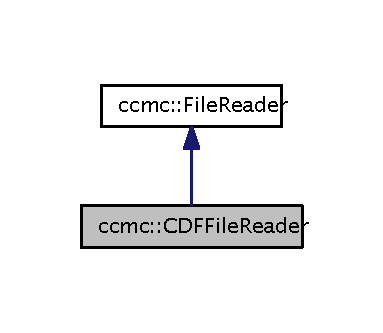
\includegraphics[width=196pt]{classccmc_1_1_c_d_f_file_reader__inherit__graph}
\end{center}
\end{figure}


Collaboration diagram for ccmc\-:\-:C\-D\-F\-File\-Reader\-:
\nopagebreak
\begin{figure}[H]
\begin{center}
\leavevmode
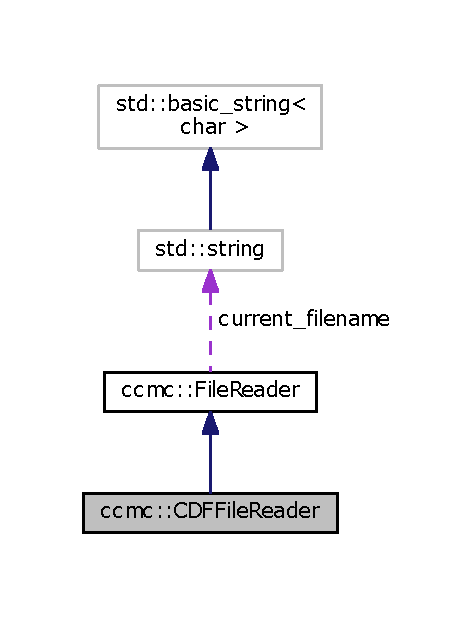
\includegraphics[width=215pt]{classccmc_1_1_c_d_f_file_reader__coll__graph}
\end{center}
\end{figure}
\subsection*{Public Member Functions}
\begin{DoxyCompactItemize}
\item 
\hyperlink{classccmc_1_1_c_d_f_file_reader_ab045259d35214f14d3064d7e0c75186b}{C\-D\-F\-File\-Reader} ()
\item 
std\-::vector$<$ float $>$ $\ast$ \hyperlink{classccmc_1_1_c_d_f_file_reader_a0d642e05bc1692134212eee14e792eab}{get\-Variable} (const std\-::string \&variable)
\begin{DoxyCompactList}\small\item\em Returns a pointer to a std\-::vector$<$float$>$ containing the values of the selected variable. \end{DoxyCompactList}\item 
std\-::vector$<$ float $>$ $\ast$ \hyperlink{classccmc_1_1_c_d_f_file_reader_a96d9e7b832f3d689217af4d54898d5c0}{get\-Variable} (long variable\-I\-D)
\item 
std\-::vector$<$ float $>$ $\ast$ \hyperlink{classccmc_1_1_c_d_f_file_reader_a24ad5f1aafad6362f98e500a9cff6412}{get\-Variable} (const std\-::string \&variable, long start\-Index, long count)
\item 
std\-::vector$<$ float $>$ $\ast$ \hyperlink{classccmc_1_1_c_d_f_file_reader_ae969f1d20235ebeb533b6d90c5497b28}{get\-Variable} (long variable\-I\-D, long start\-Index, long count)
\item 
float \hyperlink{classccmc_1_1_c_d_f_file_reader_aaf8553b84f638e02c44d6a453ce089bc}{get\-Variable\-At\-Index} (const std\-::string \&variable, long index)
\begin{DoxyCompactList}\small\item\em Returns a value in the flat array of the variable and index requested. \end{DoxyCompactList}\item 
float \hyperlink{classccmc_1_1_c_d_f_file_reader_a93d6c7e3c8587812ed8ead92f2596049}{get\-Variable\-At\-Index} (long variable\-\_\-id, long index)
\item 
std\-::vector$<$ int $>$ $\ast$ \hyperlink{classccmc_1_1_c_d_f_file_reader_a4f46a67b2469c2fb5a963e2d00fe1424}{get\-Variable\-Int} (const std\-::string \&variable)
\item 
int \hyperlink{classccmc_1_1_c_d_f_file_reader_a6a1da27717bbac69ef9eb9eaeb06f677}{get\-Variable\-Int\-At\-Index} (const std\-::string \&variable, long index)
\begin{DoxyCompactList}\small\item\em Returns a value in the flat array of the variable and index requested. \end{DoxyCompactList}\item 
int \hyperlink{classccmc_1_1_c_d_f_file_reader_a881308df42ee5d273cb7364152f6970d}{get\-Number\-Of\-Global\-Attributes} ()
\item 
int \hyperlink{classccmc_1_1_c_d_f_file_reader_ae463cfe808dec21748a908b080c8bf81}{get\-Number\-Of\-Variables} ()
\item 
int \hyperlink{classccmc_1_1_c_d_f_file_reader_aeafab3428b6ca81a9142faee44b3069f}{get\-Number\-Of\-Variable\-Attributes} ()
\item 
long \hyperlink{classccmc_1_1_c_d_f_file_reader_adc8d27cd794641171674307330ebdc66}{get\-Number\-Of\-Records} (const std\-::string \&variable)
\item 
long \hyperlink{classccmc_1_1_c_d_f_file_reader_a97f59c4e9020eb48fa460ba74b9d2535}{get\-Number\-Of\-Records} (long variable\-\_\-id)
\item 
long \hyperlink{classccmc_1_1_c_d_f_file_reader_a7c6c138eb96e5562e3a17b1691208129}{get\-Variable\-I\-D} (const std\-::string \&variable)
\item 
std\-::string \hyperlink{classccmc_1_1_c_d_f_file_reader_a98ab0f21eb5bad8b9fc095d8c1347e24}{get\-Variable\-Name} (long variable\-\_\-id)
\item 
\hyperlink{classccmc_1_1_attribute}{Attribute} \hyperlink{classccmc_1_1_c_d_f_file_reader_af7d28ab77cd25e50fcf0c1a55908331a}{get\-Global\-Attribute} (long i)
\item 
std\-::string \hyperlink{classccmc_1_1_c_d_f_file_reader_a6e6e6be5271219f6a2a45c94c89630f7}{get\-Global\-Attribute\-Name} (long attribute\-\_\-id)
\item 
std\-::string \hyperlink{classccmc_1_1_c_d_f_file_reader_adc190bdf05f4d01b465a0ff314431ebb}{get\-Variable\-Attribute\-Name} (long attribute\-\_\-id)
\item 
\hyperlink{classccmc_1_1_attribute}{Attribute} \hyperlink{classccmc_1_1_c_d_f_file_reader_aeaffff44fdcad36ae26cd7b84ba39a61}{get\-Global\-Attribute} (const std\-::string \&attribute)
\item 
\hyperlink{classccmc_1_1_attribute}{Attribute} \hyperlink{classccmc_1_1_c_d_f_file_reader_ad90a8f0f842e2dd8091c5883add375a6}{get\-Variable\-Attribute} (const std\-::string \&variable, const std\-::string \&attribute)
\item 
std\-::vector$<$ std\-::string $>$ \hyperlink{classccmc_1_1_c_d_f_file_reader_a52a904328cc0cb1ca7625c9469ca11ca}{get\-Variable\-Attribute\-Names} ()
\item 
bool \hyperlink{classccmc_1_1_c_d_f_file_reader_a2a13faebed9123459d75413e1388d6fa}{does\-Attribute\-Exist} (const std\-::string \&attribute)
\item 
bool \hyperlink{classccmc_1_1_c_d_f_file_reader_a6211014aebd161eb08dcddf7d249743a}{does\-Variable\-Exist} (const std\-::string \&variable)
\item 
bool \hyperlink{classccmc_1_1_c_d_f_file_reader_a6360eae4aeec86d95b750711fbfefcb6}{does\-Attribute\-Exist} (long attribute)
\item 
bool \hyperlink{classccmc_1_1_c_d_f_file_reader_a23a40091a6f58aaee5788d449dd87aa4}{does\-Variable\-Exist} (long variable)
\item 
const std\-::string \& \hyperlink{classccmc_1_1_c_d_f_file_reader_ab8274e8003b7700b2b860aef29a2cd6f}{get\-Current\-Filename} ()
\item 
virtual \hyperlink{classccmc_1_1_c_d_f_file_reader_a71fd30b3d6509401ea788aab46a1a142}{$\sim$\-C\-D\-F\-File\-Reader} ()
\end{DoxyCompactItemize}
\subsection*{Protected Member Functions}
\begin{DoxyCompactItemize}
\item 
long \hyperlink{classccmc_1_1_c_d_f_file_reader_a3eedaa5cdd71af7b4bf668ff3c9928ce}{close\-File} ()
\item 
long \hyperlink{classccmc_1_1_c_d_f_file_reader_a98d1d6bbd26aab8d1e285fa34179dfa8}{open\-File} (const std\-::string \&filename)
\item 
void \hyperlink{classccmc_1_1_c_d_f_file_reader_ae79ea609f0de436d1f78809668d1b84e}{initialize\-Global\-Attributes} ()
\item 
void \hyperlink{classccmc_1_1_c_d_f_file_reader_adf5fe4154607e05e6d5e8652f26c0d86}{initialize\-Variable\-Attributes} ()
\item 
void \hyperlink{classccmc_1_1_c_d_f_file_reader_a20efd34232f8348d44291b589a94d56a}{initialize\-Variable\-I\-Ds} ()
\item 
void \hyperlink{classccmc_1_1_c_d_f_file_reader_ab9c343c409df6b079c270e9598ac0fd0}{initialize\-Variable\-Names} ()
\end{DoxyCompactItemize}
\subsection*{Additional Inherited Members}


\subsection{Constructor \& Destructor Documentation}
\hypertarget{classccmc_1_1_c_d_f_file_reader_ab045259d35214f14d3064d7e0c75186b}{\index{ccmc\-::\-C\-D\-F\-File\-Reader@{ccmc\-::\-C\-D\-F\-File\-Reader}!C\-D\-F\-File\-Reader@{C\-D\-F\-File\-Reader}}
\index{C\-D\-F\-File\-Reader@{C\-D\-F\-File\-Reader}!ccmc::CDFFileReader@{ccmc\-::\-C\-D\-F\-File\-Reader}}
\subsubsection[{C\-D\-F\-File\-Reader}]{\setlength{\rightskip}{0pt plus 5cm}ccmc\-::\-C\-D\-F\-File\-Reader\-::\-C\-D\-F\-File\-Reader (
\begin{DoxyParamCaption}
{}
\end{DoxyParamCaption}
)}}\label{classccmc_1_1_c_d_f_file_reader_ab045259d35214f14d3064d7e0c75186b}
Default constructor. Does nothing. \hypertarget{classccmc_1_1_c_d_f_file_reader_a71fd30b3d6509401ea788aab46a1a142}{\index{ccmc\-::\-C\-D\-F\-File\-Reader@{ccmc\-::\-C\-D\-F\-File\-Reader}!$\sim$\-C\-D\-F\-File\-Reader@{$\sim$\-C\-D\-F\-File\-Reader}}
\index{$\sim$\-C\-D\-F\-File\-Reader@{$\sim$\-C\-D\-F\-File\-Reader}!ccmc::CDFFileReader@{ccmc\-::\-C\-D\-F\-File\-Reader}}
\subsubsection[{$\sim$\-C\-D\-F\-File\-Reader}]{\setlength{\rightskip}{0pt plus 5cm}ccmc\-::\-C\-D\-F\-File\-Reader\-::$\sim$\-C\-D\-F\-File\-Reader (
\begin{DoxyParamCaption}
{}
\end{DoxyParamCaption}
)\hspace{0.3cm}{\ttfamily [virtual]}}}\label{classccmc_1_1_c_d_f_file_reader_a71fd30b3d6509401ea788aab46a1a142}
Destructor 

\subsection{Member Function Documentation}
\hypertarget{classccmc_1_1_c_d_f_file_reader_a3eedaa5cdd71af7b4bf668ff3c9928ce}{\index{ccmc\-::\-C\-D\-F\-File\-Reader@{ccmc\-::\-C\-D\-F\-File\-Reader}!close\-File@{close\-File}}
\index{close\-File@{close\-File}!ccmc::CDFFileReader@{ccmc\-::\-C\-D\-F\-File\-Reader}}
\subsubsection[{close\-File}]{\setlength{\rightskip}{0pt plus 5cm}long ccmc\-::\-C\-D\-F\-File\-Reader\-::close\-File (
\begin{DoxyParamCaption}
{}
\end{DoxyParamCaption}
)\hspace{0.3cm}{\ttfamily [protected]}, {\ttfamily [virtual]}}}\label{classccmc_1_1_c_d_f_file_reader_a3eedaa5cdd71af7b4bf668ff3c9928ce}
Closes the currently selected file. Call this from the \hyperlink{classccmc_1_1_file_reader_a036ac2d85ad32a98b81c9e6ebf0ef133}{close()} method. \begin{DoxyReturn}{Returns}
Status of close operation. 
\end{DoxyReturn}


Implements \hyperlink{classccmc_1_1_file_reader_aa9b2ff7591f3d3f40ceb0007acbbe3ca}{ccmc\-::\-File\-Reader}.

\hypertarget{classccmc_1_1_c_d_f_file_reader_a2a13faebed9123459d75413e1388d6fa}{\index{ccmc\-::\-C\-D\-F\-File\-Reader@{ccmc\-::\-C\-D\-F\-File\-Reader}!does\-Attribute\-Exist@{does\-Attribute\-Exist}}
\index{does\-Attribute\-Exist@{does\-Attribute\-Exist}!ccmc::CDFFileReader@{ccmc\-::\-C\-D\-F\-File\-Reader}}
\subsubsection[{does\-Attribute\-Exist}]{\setlength{\rightskip}{0pt plus 5cm}bool ccmc\-::\-C\-D\-F\-File\-Reader\-::does\-Attribute\-Exist (
\begin{DoxyParamCaption}
\item[{const std\-::string \&}]{attribute}
\end{DoxyParamCaption}
)\hspace{0.3cm}{\ttfamily [virtual]}}}\label{classccmc_1_1_c_d_f_file_reader_a2a13faebed9123459d75413e1388d6fa}

\begin{DoxyParams}{Parameters}
{\em attribute} & \\
\hline
\end{DoxyParams}
\begin{DoxyReturn}{Returns}

\end{DoxyReturn}


Implements \hyperlink{classccmc_1_1_file_reader_ac27cfdd9ceabe3af0f14b18fbebcafa5}{ccmc\-::\-File\-Reader}.

\hypertarget{classccmc_1_1_c_d_f_file_reader_a6360eae4aeec86d95b750711fbfefcb6}{\index{ccmc\-::\-C\-D\-F\-File\-Reader@{ccmc\-::\-C\-D\-F\-File\-Reader}!does\-Attribute\-Exist@{does\-Attribute\-Exist}}
\index{does\-Attribute\-Exist@{does\-Attribute\-Exist}!ccmc::CDFFileReader@{ccmc\-::\-C\-D\-F\-File\-Reader}}
\subsubsection[{does\-Attribute\-Exist}]{\setlength{\rightskip}{0pt plus 5cm}bool ccmc\-::\-C\-D\-F\-File\-Reader\-::does\-Attribute\-Exist (
\begin{DoxyParamCaption}
\item[{long}]{attribute}
\end{DoxyParamCaption}
)}}\label{classccmc_1_1_c_d_f_file_reader_a6360eae4aeec86d95b750711fbfefcb6}

\begin{DoxyParams}{Parameters}
{\em attribute} & \\
\hline
\end{DoxyParams}
\begin{DoxyReturn}{Returns}

\end{DoxyReturn}
\hypertarget{classccmc_1_1_c_d_f_file_reader_a6211014aebd161eb08dcddf7d249743a}{\index{ccmc\-::\-C\-D\-F\-File\-Reader@{ccmc\-::\-C\-D\-F\-File\-Reader}!does\-Variable\-Exist@{does\-Variable\-Exist}}
\index{does\-Variable\-Exist@{does\-Variable\-Exist}!ccmc::CDFFileReader@{ccmc\-::\-C\-D\-F\-File\-Reader}}
\subsubsection[{does\-Variable\-Exist}]{\setlength{\rightskip}{0pt plus 5cm}bool ccmc\-::\-C\-D\-F\-File\-Reader\-::does\-Variable\-Exist (
\begin{DoxyParamCaption}
\item[{const std\-::string \&}]{variable}
\end{DoxyParamCaption}
)\hspace{0.3cm}{\ttfamily [virtual]}}}\label{classccmc_1_1_c_d_f_file_reader_a6211014aebd161eb08dcddf7d249743a}

\begin{DoxyParams}{Parameters}
{\em variable} & \\
\hline
\end{DoxyParams}
\begin{DoxyReturn}{Returns}

\end{DoxyReturn}


Implements \hyperlink{classccmc_1_1_file_reader_ab8893f7d2b0f62041c37a788affe6b36}{ccmc\-::\-File\-Reader}.

\hypertarget{classccmc_1_1_c_d_f_file_reader_a23a40091a6f58aaee5788d449dd87aa4}{\index{ccmc\-::\-C\-D\-F\-File\-Reader@{ccmc\-::\-C\-D\-F\-File\-Reader}!does\-Variable\-Exist@{does\-Variable\-Exist}}
\index{does\-Variable\-Exist@{does\-Variable\-Exist}!ccmc::CDFFileReader@{ccmc\-::\-C\-D\-F\-File\-Reader}}
\subsubsection[{does\-Variable\-Exist}]{\setlength{\rightskip}{0pt plus 5cm}bool ccmc\-::\-C\-D\-F\-File\-Reader\-::does\-Variable\-Exist (
\begin{DoxyParamCaption}
\item[{long}]{variable}
\end{DoxyParamCaption}
)}}\label{classccmc_1_1_c_d_f_file_reader_a23a40091a6f58aaee5788d449dd87aa4}

\begin{DoxyParams}{Parameters}
{\em variable} & \\
\hline
\end{DoxyParams}
\begin{DoxyReturn}{Returns}

\end{DoxyReturn}
\hypertarget{classccmc_1_1_c_d_f_file_reader_ab8274e8003b7700b2b860aef29a2cd6f}{\index{ccmc\-::\-C\-D\-F\-File\-Reader@{ccmc\-::\-C\-D\-F\-File\-Reader}!get\-Current\-Filename@{get\-Current\-Filename}}
\index{get\-Current\-Filename@{get\-Current\-Filename}!ccmc::CDFFileReader@{ccmc\-::\-C\-D\-F\-File\-Reader}}
\subsubsection[{get\-Current\-Filename}]{\setlength{\rightskip}{0pt plus 5cm}const std\-::string \& ccmc\-::\-C\-D\-F\-File\-Reader\-::get\-Current\-Filename (
\begin{DoxyParamCaption}
{}
\end{DoxyParamCaption}
)\hspace{0.3cm}{\ttfamily [virtual]}}}\label{classccmc_1_1_c_d_f_file_reader_ab8274e8003b7700b2b860aef29a2cd6f}
Returns the current filename. \begin{DoxyReturn}{Returns}
The current filename. 
\end{DoxyReturn}


Implements \hyperlink{classccmc_1_1_file_reader_a9f266e85464a71985e6c922ba508aa9e}{ccmc\-::\-File\-Reader}.

\hypertarget{classccmc_1_1_c_d_f_file_reader_af7d28ab77cd25e50fcf0c1a55908331a}{\index{ccmc\-::\-C\-D\-F\-File\-Reader@{ccmc\-::\-C\-D\-F\-File\-Reader}!get\-Global\-Attribute@{get\-Global\-Attribute}}
\index{get\-Global\-Attribute@{get\-Global\-Attribute}!ccmc::CDFFileReader@{ccmc\-::\-C\-D\-F\-File\-Reader}}
\subsubsection[{get\-Global\-Attribute}]{\setlength{\rightskip}{0pt plus 5cm}{\bf Attribute} ccmc\-::\-C\-D\-F\-File\-Reader\-::get\-Global\-Attribute (
\begin{DoxyParamCaption}
\item[{long}]{i}
\end{DoxyParamCaption}
)\hspace{0.3cm}{\ttfamily [virtual]}}}\label{classccmc_1_1_c_d_f_file_reader_af7d28ab77cd25e50fcf0c1a55908331a}

\begin{DoxyParams}{Parameters}
{\em i} & The attribute number \\
\hline
\end{DoxyParams}
\begin{DoxyReturn}{Returns}

\end{DoxyReturn}


Implements \hyperlink{classccmc_1_1_file_reader_a11885da1a8d6775a7d2764494474d067}{ccmc\-::\-File\-Reader}.



Here is the call graph for this function\-:
\nopagebreak
\begin{figure}[H]
\begin{center}
\leavevmode
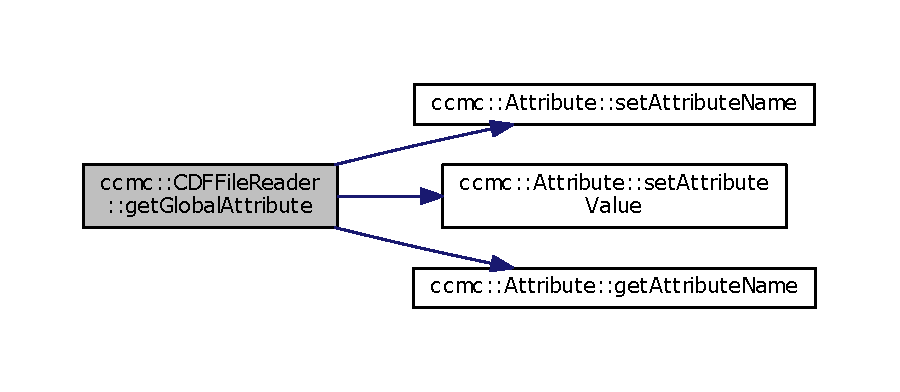
\includegraphics[width=350pt]{classccmc_1_1_c_d_f_file_reader_af7d28ab77cd25e50fcf0c1a55908331a_cgraph}
\end{center}
\end{figure}


\hypertarget{classccmc_1_1_c_d_f_file_reader_aeaffff44fdcad36ae26cd7b84ba39a61}{\index{ccmc\-::\-C\-D\-F\-File\-Reader@{ccmc\-::\-C\-D\-F\-File\-Reader}!get\-Global\-Attribute@{get\-Global\-Attribute}}
\index{get\-Global\-Attribute@{get\-Global\-Attribute}!ccmc::CDFFileReader@{ccmc\-::\-C\-D\-F\-File\-Reader}}
\subsubsection[{get\-Global\-Attribute}]{\setlength{\rightskip}{0pt plus 5cm}{\bf Attribute} ccmc\-::\-C\-D\-F\-File\-Reader\-::get\-Global\-Attribute (
\begin{DoxyParamCaption}
\item[{const std\-::string \&}]{attribute}
\end{DoxyParamCaption}
)\hspace{0.3cm}{\ttfamily [virtual]}}}\label{classccmc_1_1_c_d_f_file_reader_aeaffff44fdcad36ae26cd7b84ba39a61}

\begin{DoxyParams}{Parameters}
{\em attribute} & \\
\hline
\end{DoxyParams}
\begin{DoxyReturn}{Returns}

\end{DoxyReturn}


Implements \hyperlink{classccmc_1_1_file_reader_ac8c307cb70a6a99892e2538761867998}{ccmc\-::\-File\-Reader}.



Here is the call graph for this function\-:
\nopagebreak
\begin{figure}[H]
\begin{center}
\leavevmode
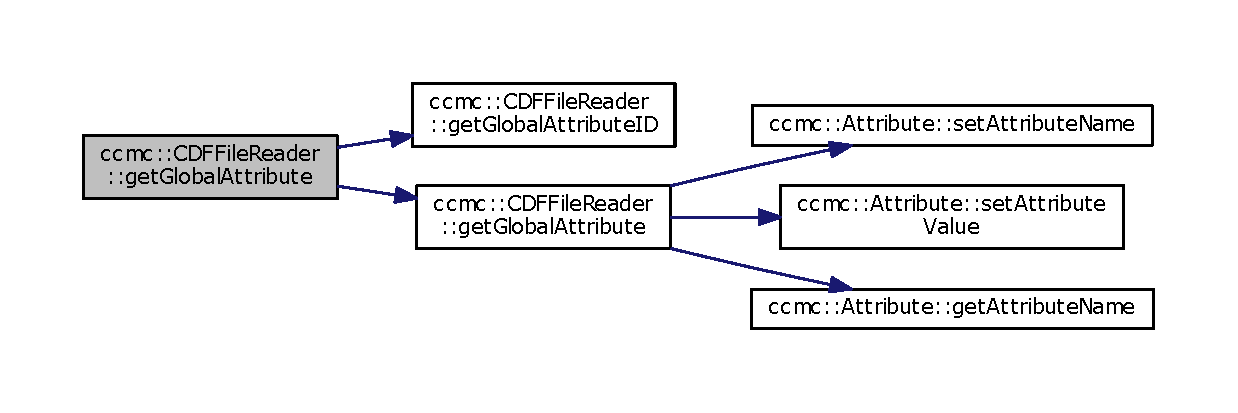
\includegraphics[width=350pt]{classccmc_1_1_c_d_f_file_reader_aeaffff44fdcad36ae26cd7b84ba39a61_cgraph}
\end{center}
\end{figure}


\hypertarget{classccmc_1_1_c_d_f_file_reader_a6e6e6be5271219f6a2a45c94c89630f7}{\index{ccmc\-::\-C\-D\-F\-File\-Reader@{ccmc\-::\-C\-D\-F\-File\-Reader}!get\-Global\-Attribute\-Name@{get\-Global\-Attribute\-Name}}
\index{get\-Global\-Attribute\-Name@{get\-Global\-Attribute\-Name}!ccmc::CDFFileReader@{ccmc\-::\-C\-D\-F\-File\-Reader}}
\subsubsection[{get\-Global\-Attribute\-Name}]{\setlength{\rightskip}{0pt plus 5cm}std\-::string ccmc\-::\-C\-D\-F\-File\-Reader\-::get\-Global\-Attribute\-Name (
\begin{DoxyParamCaption}
\item[{long}]{attribute\-\_\-id}
\end{DoxyParamCaption}
)\hspace{0.3cm}{\ttfamily [virtual]}}}\label{classccmc_1_1_c_d_f_file_reader_a6e6e6be5271219f6a2a45c94c89630f7}

\begin{DoxyParams}{Parameters}
{\em attribute\-\_\-id} & \\
\hline
\end{DoxyParams}
\begin{DoxyReturn}{Returns}

\end{DoxyReturn}


Implements \hyperlink{classccmc_1_1_file_reader_a7a4fc5909fce20cb6a40d0a1af56e9a1}{ccmc\-::\-File\-Reader}.

\hypertarget{classccmc_1_1_c_d_f_file_reader_a881308df42ee5d273cb7364152f6970d}{\index{ccmc\-::\-C\-D\-F\-File\-Reader@{ccmc\-::\-C\-D\-F\-File\-Reader}!get\-Number\-Of\-Global\-Attributes@{get\-Number\-Of\-Global\-Attributes}}
\index{get\-Number\-Of\-Global\-Attributes@{get\-Number\-Of\-Global\-Attributes}!ccmc::CDFFileReader@{ccmc\-::\-C\-D\-F\-File\-Reader}}
\subsubsection[{get\-Number\-Of\-Global\-Attributes}]{\setlength{\rightskip}{0pt plus 5cm}int ccmc\-::\-C\-D\-F\-File\-Reader\-::get\-Number\-Of\-Global\-Attributes (
\begin{DoxyParamCaption}
{}
\end{DoxyParamCaption}
)\hspace{0.3cm}{\ttfamily [virtual]}}}\label{classccmc_1_1_c_d_f_file_reader_a881308df42ee5d273cb7364152f6970d}
T\-O\-D\-O Retrieves the number of global attributes in the selected file. This is useful for iterating over all available global attributes. \begin{DoxyReturn}{Returns}
The number of global attributes stored in the selected file. 
\end{DoxyReturn}


Implements \hyperlink{classccmc_1_1_file_reader_a006779f8e665219a7de5214f4d12f80f}{ccmc\-::\-File\-Reader}.

\hypertarget{classccmc_1_1_c_d_f_file_reader_adc8d27cd794641171674307330ebdc66}{\index{ccmc\-::\-C\-D\-F\-File\-Reader@{ccmc\-::\-C\-D\-F\-File\-Reader}!get\-Number\-Of\-Records@{get\-Number\-Of\-Records}}
\index{get\-Number\-Of\-Records@{get\-Number\-Of\-Records}!ccmc::CDFFileReader@{ccmc\-::\-C\-D\-F\-File\-Reader}}
\subsubsection[{get\-Number\-Of\-Records}]{\setlength{\rightskip}{0pt plus 5cm}long ccmc\-::\-C\-D\-F\-File\-Reader\-::get\-Number\-Of\-Records (
\begin{DoxyParamCaption}
\item[{const std\-::string \&}]{variable}
\end{DoxyParamCaption}
)\hspace{0.3cm}{\ttfamily [virtual]}}}\label{classccmc_1_1_c_d_f_file_reader_adc8d27cd794641171674307330ebdc66}

\begin{DoxyParams}{Parameters}
{\em variable} & \\
\hline
\end{DoxyParams}
\begin{DoxyReturn}{Returns}

\end{DoxyReturn}


Implements \hyperlink{classccmc_1_1_file_reader_a6bed5da48bfcdf635a2f6cc71a1d5ca3}{ccmc\-::\-File\-Reader}.

\hypertarget{classccmc_1_1_c_d_f_file_reader_a97f59c4e9020eb48fa460ba74b9d2535}{\index{ccmc\-::\-C\-D\-F\-File\-Reader@{ccmc\-::\-C\-D\-F\-File\-Reader}!get\-Number\-Of\-Records@{get\-Number\-Of\-Records}}
\index{get\-Number\-Of\-Records@{get\-Number\-Of\-Records}!ccmc::CDFFileReader@{ccmc\-::\-C\-D\-F\-File\-Reader}}
\subsubsection[{get\-Number\-Of\-Records}]{\setlength{\rightskip}{0pt plus 5cm}long ccmc\-::\-C\-D\-F\-File\-Reader\-::get\-Number\-Of\-Records (
\begin{DoxyParamCaption}
\item[{long}]{variable\-\_\-id}
\end{DoxyParamCaption}
)\hspace{0.3cm}{\ttfamily [virtual]}}}\label{classccmc_1_1_c_d_f_file_reader_a97f59c4e9020eb48fa460ba74b9d2535}

\begin{DoxyParams}{Parameters}
{\em variable\-\_\-id} & \\
\hline
\end{DoxyParams}
\begin{DoxyReturn}{Returns}

\end{DoxyReturn}


Implements \hyperlink{classccmc_1_1_file_reader_a34a7240022397c1ee0efb71751ded69c}{ccmc\-::\-File\-Reader}.

\hypertarget{classccmc_1_1_c_d_f_file_reader_aeafab3428b6ca81a9142faee44b3069f}{\index{ccmc\-::\-C\-D\-F\-File\-Reader@{ccmc\-::\-C\-D\-F\-File\-Reader}!get\-Number\-Of\-Variable\-Attributes@{get\-Number\-Of\-Variable\-Attributes}}
\index{get\-Number\-Of\-Variable\-Attributes@{get\-Number\-Of\-Variable\-Attributes}!ccmc::CDFFileReader@{ccmc\-::\-C\-D\-F\-File\-Reader}}
\subsubsection[{get\-Number\-Of\-Variable\-Attributes}]{\setlength{\rightskip}{0pt plus 5cm}int ccmc\-::\-C\-D\-F\-File\-Reader\-::get\-Number\-Of\-Variable\-Attributes (
\begin{DoxyParamCaption}
{}
\end{DoxyParamCaption}
)\hspace{0.3cm}{\ttfamily [virtual]}}}\label{classccmc_1_1_c_d_f_file_reader_aeafab3428b6ca81a9142faee44b3069f}
Gets the number of variable attributes. \begin{DoxyReturn}{Returns}
The number of variable attributes in the opened file. 
\end{DoxyReturn}


Implements \hyperlink{classccmc_1_1_file_reader_ad5c3584515c7f2896b49af21b2b15890}{ccmc\-::\-File\-Reader}.

\hypertarget{classccmc_1_1_c_d_f_file_reader_ae463cfe808dec21748a908b080c8bf81}{\index{ccmc\-::\-C\-D\-F\-File\-Reader@{ccmc\-::\-C\-D\-F\-File\-Reader}!get\-Number\-Of\-Variables@{get\-Number\-Of\-Variables}}
\index{get\-Number\-Of\-Variables@{get\-Number\-Of\-Variables}!ccmc::CDFFileReader@{ccmc\-::\-C\-D\-F\-File\-Reader}}
\subsubsection[{get\-Number\-Of\-Variables}]{\setlength{\rightskip}{0pt plus 5cm}int ccmc\-::\-C\-D\-F\-File\-Reader\-::get\-Number\-Of\-Variables (
\begin{DoxyParamCaption}
{}
\end{DoxyParamCaption}
)\hspace{0.3cm}{\ttfamily [virtual]}}}\label{classccmc_1_1_c_d_f_file_reader_ae463cfe808dec21748a908b080c8bf81}
\begin{DoxyReturn}{Returns}

\end{DoxyReturn}


Implements \hyperlink{classccmc_1_1_file_reader_adf9f77e1e774cd1873648cde6ba0e479}{ccmc\-::\-File\-Reader}.

\hypertarget{classccmc_1_1_c_d_f_file_reader_a0d642e05bc1692134212eee14e792eab}{\index{ccmc\-::\-C\-D\-F\-File\-Reader@{ccmc\-::\-C\-D\-F\-File\-Reader}!get\-Variable@{get\-Variable}}
\index{get\-Variable@{get\-Variable}!ccmc::CDFFileReader@{ccmc\-::\-C\-D\-F\-File\-Reader}}
\subsubsection[{get\-Variable}]{\setlength{\rightskip}{0pt plus 5cm}std\-::vector$<$ float $>$ $\ast$ ccmc\-::\-C\-D\-F\-File\-Reader\-::get\-Variable (
\begin{DoxyParamCaption}
\item[{const std\-::string \&}]{variable}
\end{DoxyParamCaption}
)\hspace{0.3cm}{\ttfamily [virtual]}}}\label{classccmc_1_1_c_d_f_file_reader_a0d642e05bc1692134212eee14e792eab}


Returns a pointer to a std\-::vector$<$float$>$ containing the values of the selected variable. 

This allocates a new std\-::vector$<$float$>$ pointer. Make sure you delete the contents when you done using it, or you will have a memory leak.


\begin{DoxyParams}{Parameters}
{\em variable} & \\
\hline
\end{DoxyParams}
\begin{DoxyReturn}{Returns}
std\-::vector$<$float$>$ containing the values of the selected variable. 
\end{DoxyReturn}


Implements \hyperlink{classccmc_1_1_file_reader_a3703180de2d7d38c1ccf115d5279d4d0}{ccmc\-::\-File\-Reader}.



Here is the call graph for this function\-:
\nopagebreak
\begin{figure}[H]
\begin{center}
\leavevmode
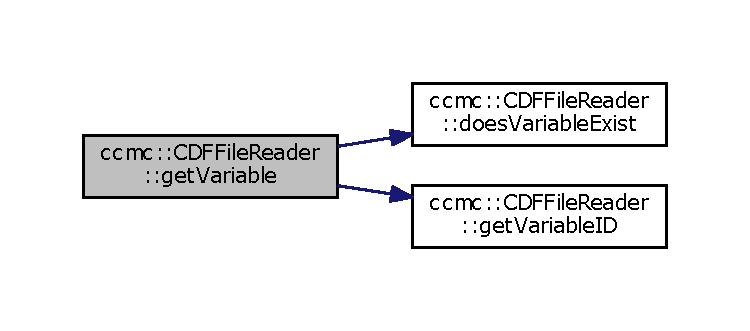
\includegraphics[width=348pt]{classccmc_1_1_c_d_f_file_reader_a0d642e05bc1692134212eee14e792eab_cgraph}
\end{center}
\end{figure}


\hypertarget{classccmc_1_1_c_d_f_file_reader_a96d9e7b832f3d689217af4d54898d5c0}{\index{ccmc\-::\-C\-D\-F\-File\-Reader@{ccmc\-::\-C\-D\-F\-File\-Reader}!get\-Variable@{get\-Variable}}
\index{get\-Variable@{get\-Variable}!ccmc::CDFFileReader@{ccmc\-::\-C\-D\-F\-File\-Reader}}
\subsubsection[{get\-Variable}]{\setlength{\rightskip}{0pt plus 5cm}std\-::vector$<$ float $>$ $\ast$ ccmc\-::\-C\-D\-F\-File\-Reader\-::get\-Variable (
\begin{DoxyParamCaption}
\item[{long}]{variable}
\end{DoxyParamCaption}
)\hspace{0.3cm}{\ttfamily [virtual]}}}\label{classccmc_1_1_c_d_f_file_reader_a96d9e7b832f3d689217af4d54898d5c0}
Returns a pointer to a std\-::vector$<$float$>$ containing the values of the selected variable stored in the selected file. This allocates a new std\-::vector$<$float$>$ pointer. Make sure you delete the contents when you done using it, or you will have a memory leak. 
\begin{DoxyParams}{Parameters}
{\em variable} & \\
\hline
\end{DoxyParams}
\begin{DoxyReturn}{Returns}
std\-::vector$<$float$>$ containing the values of the selected variable. 
\end{DoxyReturn}


Implements \hyperlink{classccmc_1_1_file_reader_a47fafa0e59e4d5f379a48b3d0b1add6e}{ccmc\-::\-File\-Reader}.



Here is the call graph for this function\-:
\nopagebreak
\begin{figure}[H]
\begin{center}
\leavevmode
\includegraphics[width=348pt]{classccmc_1_1_c_d_f_file_reader_a96d9e7b832f3d689217af4d54898d5c0_cgraph}
\end{center}
\end{figure}


\hypertarget{classccmc_1_1_c_d_f_file_reader_a24ad5f1aafad6362f98e500a9cff6412}{\index{ccmc\-::\-C\-D\-F\-File\-Reader@{ccmc\-::\-C\-D\-F\-File\-Reader}!get\-Variable@{get\-Variable}}
\index{get\-Variable@{get\-Variable}!ccmc::CDFFileReader@{ccmc\-::\-C\-D\-F\-File\-Reader}}
\subsubsection[{get\-Variable}]{\setlength{\rightskip}{0pt plus 5cm}std\-::vector$<$ float $>$ $\ast$ ccmc\-::\-C\-D\-F\-File\-Reader\-::get\-Variable (
\begin{DoxyParamCaption}
\item[{const std\-::string \&}]{variable, }
\item[{long}]{start\-Index, }
\item[{long}]{count}
\end{DoxyParamCaption}
)\hspace{0.3cm}{\ttfamily [virtual]}}}\label{classccmc_1_1_c_d_f_file_reader_a24ad5f1aafad6362f98e500a9cff6412}
Returns a pointer to a std\-::vector$<$float$>$ containing the values of the selected variable in the range specified by the start\-Index and count (the number of records to read) stored in the selected file. This allocates a new std\-::vector$<$float$>$ pointer. Make sure you delete the contents when you done using it, or you will have a memory leak. 
\begin{DoxyParams}{Parameters}
{\em variable} & \\
\hline
{\em start\-Index} & \\
\hline
{\em count} & \\
\hline
\end{DoxyParams}
\begin{DoxyReturn}{Returns}
std\-::vector$<$float$>$ containing the values of the selected variable. 
\end{DoxyReturn}


Implements \hyperlink{classccmc_1_1_file_reader_ac8e5796569d9e7df92d6f06edf4d1d79}{ccmc\-::\-File\-Reader}.



Here is the call graph for this function\-:
\nopagebreak
\begin{figure}[H]
\begin{center}
\leavevmode
\includegraphics[width=348pt]{classccmc_1_1_c_d_f_file_reader_a24ad5f1aafad6362f98e500a9cff6412_cgraph}
\end{center}
\end{figure}


\hypertarget{classccmc_1_1_c_d_f_file_reader_ae969f1d20235ebeb533b6d90c5497b28}{\index{ccmc\-::\-C\-D\-F\-File\-Reader@{ccmc\-::\-C\-D\-F\-File\-Reader}!get\-Variable@{get\-Variable}}
\index{get\-Variable@{get\-Variable}!ccmc::CDFFileReader@{ccmc\-::\-C\-D\-F\-File\-Reader}}
\subsubsection[{get\-Variable}]{\setlength{\rightskip}{0pt plus 5cm}std\-::vector$<$ float $>$ $\ast$ ccmc\-::\-C\-D\-F\-File\-Reader\-::get\-Variable (
\begin{DoxyParamCaption}
\item[{long}]{variable, }
\item[{long}]{start\-Index, }
\item[{long}]{count}
\end{DoxyParamCaption}
)\hspace{0.3cm}{\ttfamily [virtual]}}}\label{classccmc_1_1_c_d_f_file_reader_ae969f1d20235ebeb533b6d90c5497b28}
Returns a pointer to a std\-::vector$<$float$>$ containing the values of the selected variable in the range specified by the start\-Index and count (the number of records to read) stored in the selected file. This allocates a new std\-::vector$<$float$>$ pointer. Make sure you delete the contents when you done using it, or you will have a memory leak. 
\begin{DoxyParams}{Parameters}
{\em variable\-I\-D} & \\
\hline
{\em start\-Index} & \\
\hline
{\em count} & \\
\hline
\end{DoxyParams}
\begin{DoxyReturn}{Returns}
std\-::vector$<$float$>$ containing the values of the selected variable. 
\end{DoxyReturn}


Implements \hyperlink{classccmc_1_1_file_reader_a6c127caf47837d72fa46cf5f079399dd}{ccmc\-::\-File\-Reader}.



Here is the call graph for this function\-:
\nopagebreak
\begin{figure}[H]
\begin{center}
\leavevmode
\includegraphics[width=348pt]{classccmc_1_1_c_d_f_file_reader_ae969f1d20235ebeb533b6d90c5497b28_cgraph}
\end{center}
\end{figure}


\hypertarget{classccmc_1_1_c_d_f_file_reader_aaf8553b84f638e02c44d6a453ce089bc}{\index{ccmc\-::\-C\-D\-F\-File\-Reader@{ccmc\-::\-C\-D\-F\-File\-Reader}!get\-Variable\-At\-Index@{get\-Variable\-At\-Index}}
\index{get\-Variable\-At\-Index@{get\-Variable\-At\-Index}!ccmc::CDFFileReader@{ccmc\-::\-C\-D\-F\-File\-Reader}}
\subsubsection[{get\-Variable\-At\-Index}]{\setlength{\rightskip}{0pt plus 5cm}float ccmc\-::\-C\-D\-F\-File\-Reader\-::get\-Variable\-At\-Index (
\begin{DoxyParamCaption}
\item[{const std\-::string \&}]{variable, }
\item[{long}]{index}
\end{DoxyParamCaption}
)\hspace{0.3cm}{\ttfamily [virtual]}}}\label{classccmc_1_1_c_d_f_file_reader_aaf8553b84f638e02c44d6a453ce089bc}


Returns a value in the flat array of the variable and index requested. 

Use this method on variables that have a type of float


\begin{DoxyParams}{Parameters}
{\em variable} & The variable in the file \\
\hline
{\em index} & The index in the variable's array in the file\\
\hline
\end{DoxyParams}
\begin{DoxyReturn}{Returns}
float of the value in the array. 
\end{DoxyReturn}


Implements \hyperlink{classccmc_1_1_file_reader_afb0680751b96215f3ba350b290b62f35}{ccmc\-::\-File\-Reader}.

\hypertarget{classccmc_1_1_c_d_f_file_reader_a93d6c7e3c8587812ed8ead92f2596049}{\index{ccmc\-::\-C\-D\-F\-File\-Reader@{ccmc\-::\-C\-D\-F\-File\-Reader}!get\-Variable\-At\-Index@{get\-Variable\-At\-Index}}
\index{get\-Variable\-At\-Index@{get\-Variable\-At\-Index}!ccmc::CDFFileReader@{ccmc\-::\-C\-D\-F\-File\-Reader}}
\subsubsection[{get\-Variable\-At\-Index}]{\setlength{\rightskip}{0pt plus 5cm}float ccmc\-::\-C\-D\-F\-File\-Reader\-::get\-Variable\-At\-Index (
\begin{DoxyParamCaption}
\item[{long}]{variable\-Num, }
\item[{long}]{index}
\end{DoxyParamCaption}
)\hspace{0.3cm}{\ttfamily [virtual]}}}\label{classccmc_1_1_c_d_f_file_reader_a93d6c7e3c8587812ed8ead92f2596049}

\begin{DoxyParams}{Parameters}
{\em variable\-Num} & \\
\hline
{\em index} & \\
\hline
\end{DoxyParams}
\begin{DoxyReturn}{Returns}

\end{DoxyReturn}


Implements \hyperlink{classccmc_1_1_file_reader_acfe13750b7afba1cb59925e6073f1731}{ccmc\-::\-File\-Reader}.

\hypertarget{classccmc_1_1_c_d_f_file_reader_ad90a8f0f842e2dd8091c5883add375a6}{\index{ccmc\-::\-C\-D\-F\-File\-Reader@{ccmc\-::\-C\-D\-F\-File\-Reader}!get\-Variable\-Attribute@{get\-Variable\-Attribute}}
\index{get\-Variable\-Attribute@{get\-Variable\-Attribute}!ccmc::CDFFileReader@{ccmc\-::\-C\-D\-F\-File\-Reader}}
\subsubsection[{get\-Variable\-Attribute}]{\setlength{\rightskip}{0pt plus 5cm}{\bf Attribute} ccmc\-::\-C\-D\-F\-File\-Reader\-::get\-Variable\-Attribute (
\begin{DoxyParamCaption}
\item[{const std\-::string \&}]{variable, }
\item[{const std\-::string \&}]{vattribute}
\end{DoxyParamCaption}
)\hspace{0.3cm}{\ttfamily [virtual]}}}\label{classccmc_1_1_c_d_f_file_reader_ad90a8f0f842e2dd8091c5883add375a6}

\begin{DoxyParams}{Parameters}
{\em variable} & \\
\hline
{\em vattribute} & \\
\hline
\end{DoxyParams}
\begin{DoxyReturn}{Returns}

\end{DoxyReturn}


Implements \hyperlink{classccmc_1_1_file_reader_ada8128e0f00555a8911be5e95ec18b6e}{ccmc\-::\-File\-Reader}.



Here is the call graph for this function\-:
\nopagebreak
\begin{figure}[H]
\begin{center}
\leavevmode
\includegraphics[width=350pt]{classccmc_1_1_c_d_f_file_reader_ad90a8f0f842e2dd8091c5883add375a6_cgraph}
\end{center}
\end{figure}


\hypertarget{classccmc_1_1_c_d_f_file_reader_adc190bdf05f4d01b465a0ff314431ebb}{\index{ccmc\-::\-C\-D\-F\-File\-Reader@{ccmc\-::\-C\-D\-F\-File\-Reader}!get\-Variable\-Attribute\-Name@{get\-Variable\-Attribute\-Name}}
\index{get\-Variable\-Attribute\-Name@{get\-Variable\-Attribute\-Name}!ccmc::CDFFileReader@{ccmc\-::\-C\-D\-F\-File\-Reader}}
\subsubsection[{get\-Variable\-Attribute\-Name}]{\setlength{\rightskip}{0pt plus 5cm}std\-::string ccmc\-::\-C\-D\-F\-File\-Reader\-::get\-Variable\-Attribute\-Name (
\begin{DoxyParamCaption}
\item[{long}]{attribute\-\_\-id}
\end{DoxyParamCaption}
)\hspace{0.3cm}{\ttfamily [virtual]}}}\label{classccmc_1_1_c_d_f_file_reader_adc190bdf05f4d01b465a0ff314431ebb}

\begin{DoxyParams}{Parameters}
{\em attribute\-\_\-id} & \\
\hline
\end{DoxyParams}
\begin{DoxyReturn}{Returns}
String representing the name of the attribute specified by attribute\-\_\-id 
\end{DoxyReturn}


Implements \hyperlink{classccmc_1_1_file_reader_ab901c44fdd1d8f7d4fac85f0747750ee}{ccmc\-::\-File\-Reader}.

\hypertarget{classccmc_1_1_c_d_f_file_reader_a52a904328cc0cb1ca7625c9469ca11ca}{\index{ccmc\-::\-C\-D\-F\-File\-Reader@{ccmc\-::\-C\-D\-F\-File\-Reader}!get\-Variable\-Attribute\-Names@{get\-Variable\-Attribute\-Names}}
\index{get\-Variable\-Attribute\-Names@{get\-Variable\-Attribute\-Names}!ccmc::CDFFileReader@{ccmc\-::\-C\-D\-F\-File\-Reader}}
\subsubsection[{get\-Variable\-Attribute\-Names}]{\setlength{\rightskip}{0pt plus 5cm}std\-::vector$<$ std\-::string $>$ ccmc\-::\-C\-D\-F\-File\-Reader\-::get\-Variable\-Attribute\-Names (
\begin{DoxyParamCaption}
{}
\end{DoxyParamCaption}
)\hspace{0.3cm}{\ttfamily [virtual]}}}\label{classccmc_1_1_c_d_f_file_reader_a52a904328cc0cb1ca7625c9469ca11ca}
\begin{DoxyReturn}{Returns}

\end{DoxyReturn}


Implements \hyperlink{classccmc_1_1_file_reader_a6f11a946eac2b10674e948a3c3785966}{ccmc\-::\-File\-Reader}.

\hypertarget{classccmc_1_1_c_d_f_file_reader_a7c6c138eb96e5562e3a17b1691208129}{\index{ccmc\-::\-C\-D\-F\-File\-Reader@{ccmc\-::\-C\-D\-F\-File\-Reader}!get\-Variable\-I\-D@{get\-Variable\-I\-D}}
\index{get\-Variable\-I\-D@{get\-Variable\-I\-D}!ccmc::CDFFileReader@{ccmc\-::\-C\-D\-F\-File\-Reader}}
\subsubsection[{get\-Variable\-I\-D}]{\setlength{\rightskip}{0pt plus 5cm}long ccmc\-::\-C\-D\-F\-File\-Reader\-::get\-Variable\-I\-D (
\begin{DoxyParamCaption}
\item[{const std\-::string \&}]{variable}
\end{DoxyParamCaption}
)\hspace{0.3cm}{\ttfamily [virtual]}}}\label{classccmc_1_1_c_d_f_file_reader_a7c6c138eb96e5562e3a17b1691208129}
Returns the variable I\-D as a long. Using the variable I\-D wherever possible is significantly faster than the equivalent methods accepting the variable string. \begin{DoxyReturn}{Returns}
Status of the file operation. 
\end{DoxyReturn}


Implements \hyperlink{classccmc_1_1_file_reader_a937185c6d323262f7c3f3c4d39b59e37}{ccmc\-::\-File\-Reader}.

\hypertarget{classccmc_1_1_c_d_f_file_reader_a4f46a67b2469c2fb5a963e2d00fe1424}{\index{ccmc\-::\-C\-D\-F\-File\-Reader@{ccmc\-::\-C\-D\-F\-File\-Reader}!get\-Variable\-Int@{get\-Variable\-Int}}
\index{get\-Variable\-Int@{get\-Variable\-Int}!ccmc::CDFFileReader@{ccmc\-::\-C\-D\-F\-File\-Reader}}
\subsubsection[{get\-Variable\-Int}]{\setlength{\rightskip}{0pt plus 5cm}std\-::vector$<$ int $>$ $\ast$ ccmc\-::\-C\-D\-F\-File\-Reader\-::get\-Variable\-Int (
\begin{DoxyParamCaption}
\item[{const std\-::string \&}]{variable}
\end{DoxyParamCaption}
)\hspace{0.3cm}{\ttfamily [virtual]}}}\label{classccmc_1_1_c_d_f_file_reader_a4f46a67b2469c2fb5a963e2d00fe1424}
This allocates a new std\-::vector$<$int$>$ pointer. Make sure you delete the contents when you done using it, or you will have a memory leak. 
\begin{DoxyParams}{Parameters}
{\em variable} & \\
\hline
\end{DoxyParams}
\begin{DoxyReturn}{Returns}
vector$<$int$>$ containing the integer values of the variable 
\end{DoxyReturn}


Implements \hyperlink{classccmc_1_1_file_reader_ab8f4f917ca18681189e3ac8001282c34}{ccmc\-::\-File\-Reader}.



Here is the call graph for this function\-:
\nopagebreak
\begin{figure}[H]
\begin{center}
\leavevmode
\includegraphics[width=348pt]{classccmc_1_1_c_d_f_file_reader_a4f46a67b2469c2fb5a963e2d00fe1424_cgraph}
\end{center}
\end{figure}


\hypertarget{classccmc_1_1_c_d_f_file_reader_a6a1da27717bbac69ef9eb9eaeb06f677}{\index{ccmc\-::\-C\-D\-F\-File\-Reader@{ccmc\-::\-C\-D\-F\-File\-Reader}!get\-Variable\-Int\-At\-Index@{get\-Variable\-Int\-At\-Index}}
\index{get\-Variable\-Int\-At\-Index@{get\-Variable\-Int\-At\-Index}!ccmc::CDFFileReader@{ccmc\-::\-C\-D\-F\-File\-Reader}}
\subsubsection[{get\-Variable\-Int\-At\-Index}]{\setlength{\rightskip}{0pt plus 5cm}int ccmc\-::\-C\-D\-F\-File\-Reader\-::get\-Variable\-Int\-At\-Index (
\begin{DoxyParamCaption}
\item[{const std\-::string \&}]{variable, }
\item[{long}]{index}
\end{DoxyParamCaption}
)\hspace{0.3cm}{\ttfamily [virtual]}}}\label{classccmc_1_1_c_d_f_file_reader_a6a1da27717bbac69ef9eb9eaeb06f677}


Returns a value in the flat array of the variable and index requested. 

Use this method on variables that have a type of int


\begin{DoxyParams}{Parameters}
{\em variable} & The variable in the file \\
\hline
{\em index} & The index in the variable's array in the file\\
\hline
\end{DoxyParams}
\begin{DoxyReturn}{Returns}
int of the value in the array. 
\end{DoxyReturn}


Implements \hyperlink{classccmc_1_1_file_reader_a1ef9e0b43e1a3f051ceea507f00598f5}{ccmc\-::\-File\-Reader}.

\hypertarget{classccmc_1_1_c_d_f_file_reader_a98ab0f21eb5bad8b9fc095d8c1347e24}{\index{ccmc\-::\-C\-D\-F\-File\-Reader@{ccmc\-::\-C\-D\-F\-File\-Reader}!get\-Variable\-Name@{get\-Variable\-Name}}
\index{get\-Variable\-Name@{get\-Variable\-Name}!ccmc::CDFFileReader@{ccmc\-::\-C\-D\-F\-File\-Reader}}
\subsubsection[{get\-Variable\-Name}]{\setlength{\rightskip}{0pt plus 5cm}std\-::string ccmc\-::\-C\-D\-F\-File\-Reader\-::get\-Variable\-Name (
\begin{DoxyParamCaption}
\item[{long}]{variable\-\_\-id}
\end{DoxyParamCaption}
)\hspace{0.3cm}{\ttfamily [virtual]}}}\label{classccmc_1_1_c_d_f_file_reader_a98ab0f21eb5bad8b9fc095d8c1347e24}
Returns the string representation of the variable referred to by variable\-\_\-id \begin{DoxyReturn}{Returns}
String representation of the variable. 
\end{DoxyReturn}


Implements \hyperlink{classccmc_1_1_file_reader_af688dd7824a25f91404e5f586d1ebe86}{ccmc\-::\-File\-Reader}.

\hypertarget{classccmc_1_1_c_d_f_file_reader_ae79ea609f0de436d1f78809668d1b84e}{\index{ccmc\-::\-C\-D\-F\-File\-Reader@{ccmc\-::\-C\-D\-F\-File\-Reader}!initialize\-Global\-Attributes@{initialize\-Global\-Attributes}}
\index{initialize\-Global\-Attributes@{initialize\-Global\-Attributes}!ccmc::CDFFileReader@{ccmc\-::\-C\-D\-F\-File\-Reader}}
\subsubsection[{initialize\-Global\-Attributes}]{\setlength{\rightskip}{0pt plus 5cm}void ccmc\-::\-C\-D\-F\-File\-Reader\-::initialize\-Global\-Attributes (
\begin{DoxyParamCaption}
{}
\end{DoxyParamCaption}
)\hspace{0.3cm}{\ttfamily [protected]}}}\label{classccmc_1_1_c_d_f_file_reader_ae79ea609f0de436d1f78809668d1b84e}
Helper method to store the global attributes in a map. This solves some issues with threaded operations on C\-D\-F files. 

Reimplemented from \hyperlink{classccmc_1_1_file_reader_a38580b9175bb58240630ed1c98147209}{ccmc\-::\-File\-Reader}.

\hypertarget{classccmc_1_1_c_d_f_file_reader_adf5fe4154607e05e6d5e8652f26c0d86}{\index{ccmc\-::\-C\-D\-F\-File\-Reader@{ccmc\-::\-C\-D\-F\-File\-Reader}!initialize\-Variable\-Attributes@{initialize\-Variable\-Attributes}}
\index{initialize\-Variable\-Attributes@{initialize\-Variable\-Attributes}!ccmc::CDFFileReader@{ccmc\-::\-C\-D\-F\-File\-Reader}}
\subsubsection[{initialize\-Variable\-Attributes}]{\setlength{\rightskip}{0pt plus 5cm}void ccmc\-::\-C\-D\-F\-File\-Reader\-::initialize\-Variable\-Attributes (
\begin{DoxyParamCaption}
{}
\end{DoxyParamCaption}
)\hspace{0.3cm}{\ttfamily [protected]}}}\label{classccmc_1_1_c_d_f_file_reader_adf5fe4154607e05e6d5e8652f26c0d86}


Reimplemented from \hyperlink{classccmc_1_1_file_reader_a9a5bc837ba6c1ccba7543fe934b9879b}{ccmc\-::\-File\-Reader}.

\hypertarget{classccmc_1_1_c_d_f_file_reader_a20efd34232f8348d44291b589a94d56a}{\index{ccmc\-::\-C\-D\-F\-File\-Reader@{ccmc\-::\-C\-D\-F\-File\-Reader}!initialize\-Variable\-I\-Ds@{initialize\-Variable\-I\-Ds}}
\index{initialize\-Variable\-I\-Ds@{initialize\-Variable\-I\-Ds}!ccmc::CDFFileReader@{ccmc\-::\-C\-D\-F\-File\-Reader}}
\subsubsection[{initialize\-Variable\-I\-Ds}]{\setlength{\rightskip}{0pt plus 5cm}void ccmc\-::\-C\-D\-F\-File\-Reader\-::initialize\-Variable\-I\-Ds (
\begin{DoxyParamCaption}
{}
\end{DoxyParamCaption}
)\hspace{0.3cm}{\ttfamily [protected]}, {\ttfamily [virtual]}}}\label{classccmc_1_1_c_d_f_file_reader_a20efd34232f8348d44291b589a94d56a}
Helper method to initialize a map containing variable I\-Ds. This solves some issues with threaded operations on C\-D\-F files. 

Implements \hyperlink{classccmc_1_1_file_reader_a2663bad21fc69c24f555b27d1cc2b8c8}{ccmc\-::\-File\-Reader}.

\hypertarget{classccmc_1_1_c_d_f_file_reader_ab9c343c409df6b079c270e9598ac0fd0}{\index{ccmc\-::\-C\-D\-F\-File\-Reader@{ccmc\-::\-C\-D\-F\-File\-Reader}!initialize\-Variable\-Names@{initialize\-Variable\-Names}}
\index{initialize\-Variable\-Names@{initialize\-Variable\-Names}!ccmc::CDFFileReader@{ccmc\-::\-C\-D\-F\-File\-Reader}}
\subsubsection[{initialize\-Variable\-Names}]{\setlength{\rightskip}{0pt plus 5cm}void ccmc\-::\-C\-D\-F\-File\-Reader\-::initialize\-Variable\-Names (
\begin{DoxyParamCaption}
{}
\end{DoxyParamCaption}
)\hspace{0.3cm}{\ttfamily [protected]}, {\ttfamily [virtual]}}}\label{classccmc_1_1_c_d_f_file_reader_ab9c343c409df6b079c270e9598ac0fd0}
Helper method to initialize a variable names map. This solves some issues with threaded operations on C\-D\-F files. 

Implements \hyperlink{classccmc_1_1_file_reader_a3517b66817277210916f6e5aa3db21a8}{ccmc\-::\-File\-Reader}.

\hypertarget{classccmc_1_1_c_d_f_file_reader_a98d1d6bbd26aab8d1e285fa34179dfa8}{\index{ccmc\-::\-C\-D\-F\-File\-Reader@{ccmc\-::\-C\-D\-F\-File\-Reader}!open\-File@{open\-File}}
\index{open\-File@{open\-File}!ccmc::CDFFileReader@{ccmc\-::\-C\-D\-F\-File\-Reader}}
\subsubsection[{open\-File}]{\setlength{\rightskip}{0pt plus 5cm}long ccmc\-::\-C\-D\-F\-File\-Reader\-::open\-File (
\begin{DoxyParamCaption}
\item[{const std\-::string \&}]{filename}
\end{DoxyParamCaption}
)\hspace{0.3cm}{\ttfamily [protected]}, {\ttfamily [virtual]}}}\label{classccmc_1_1_c_d_f_file_reader_a98d1d6bbd26aab8d1e285fa34179dfa8}
Opens a new file. If the previous file has been opened successfuly, and has the same filename as the requested filename, nothing will be done. 
\begin{DoxyParams}{Parameters}
{\em filename} & \\
\hline
\end{DoxyParams}
\begin{DoxyReturn}{Returns}
The status of the open call. This method should be called from \hyperlink{classccmc_1_1_file_reader_a932f3df08ebbcdf4527be1908fec118c}{open()}. 
\end{DoxyReturn}


Implements \hyperlink{classccmc_1_1_file_reader_aa4afaba431365ecd756641e479140768}{ccmc\-::\-File\-Reader}.



Here is the call graph for this function\-:
\nopagebreak
\begin{figure}[H]
\begin{center}
\leavevmode
\includegraphics[width=350pt]{classccmc_1_1_c_d_f_file_reader_a98d1d6bbd26aab8d1e285fa34179dfa8_cgraph}
\end{center}
\end{figure}




The documentation for this class was generated from the following files\-:\begin{DoxyCompactItemize}
\item 
/\-Users/dberrios/\-Documents/workspace/kameleon-\/plus/src/ccmc/\hyperlink{_c_d_f_file_reader_8h}{C\-D\-F\-File\-Reader.\-h}\item 
/\-Users/dberrios/\-Documents/workspace/kameleon-\/plus/src/ccmc/\hyperlink{_c_d_f_file_reader_8cpp}{C\-D\-F\-File\-Reader.\-cpp}\end{DoxyCompactItemize}

\hypertarget{classccmc_1_1_c_t_i_p}{\section{ccmc\-:\-:C\-T\-I\-P Class Reference}
\label{classccmc_1_1_c_t_i_p}\index{ccmc\-::\-C\-T\-I\-P@{ccmc\-::\-C\-T\-I\-P}}
}


T\-O\-D\-O\-: Brief description of \hyperlink{classccmc_1_1_c_t_i_p}{C\-T\-I\-P} class.  




{\ttfamily \#include $<$ccmc/\-C\-T\-I\-P.\-h$>$}



Inheritance diagram for ccmc\-:\-:C\-T\-I\-P\-:\nopagebreak
\begin{figure}[H]
\begin{center}
\leavevmode
\includegraphics[width=198pt]{classccmc_1_1_c_t_i_p__inherit__graph}
\end{center}
\end{figure}


Collaboration diagram for ccmc\-:\-:C\-T\-I\-P\-:\nopagebreak
\begin{figure}[H]
\begin{center}
\leavevmode
\includegraphics[width=325pt]{classccmc_1_1_c_t_i_p__coll__graph}
\end{center}
\end{figure}
\subsection*{Public Member Functions}
\begin{DoxyCompactItemize}
\item 
\hyperlink{classccmc_1_1_c_t_i_p_ad443922ade80ec2a2c170976299006c6}{C\-T\-I\-P} ()
\item 
long \hyperlink{classccmc_1_1_c_t_i_p_a2771b8d2ef4f22425f3e460ed5a9e671}{open} (const std\-::string \&filename)
\begin{DoxyCompactList}\small\item\em Opens a file.  \end{DoxyCompactList}\item 
\hyperlink{classccmc_1_1_interpolator}{Interpolator} $\ast$ \hyperlink{classccmc_1_1_c_t_i_p_a1efb34250bf5ef2eebac5ef68fe446f9}{create\-New\-Interpolator} ()
\begin{DoxyCompactList}\small\item\em Returns an \hyperlink{classccmc_1_1_interpolator}{Interpolator} object for the currently opened file.  \end{DoxyCompactList}\item 
virtual \hyperlink{classccmc_1_1_c_t_i_p_a74bd2c42b1dbe07e8ce1d2fcca5ada35}{$\sim$\-C\-T\-I\-P} ()
\end{DoxyCompactItemize}
\subsection*{Protected Member Functions}
\begin{DoxyCompactItemize}
\item 
void \hyperlink{classccmc_1_1_c_t_i_p_a082ab812295cbbbd31a8a60d723ca518}{initialize\-Conversion\-Factors\-To\-S\-I} ()
\begin{DoxyCompactList}\small\item\em Initializes the conversion\-Factors\-To\-S\-I map.  \end{DoxyCompactList}\item 
void \hyperlink{classccmc_1_1_c_t_i_p_abcd6a28de17688978f7cee2e7798f9e8}{initialize\-S\-I\-Units} ()
\begin{DoxyCompactList}\small\item\em Initializes the variable\-S\-I\-Units map.  \end{DoxyCompactList}\end{DoxyCompactItemize}
\subsection*{Additional Inherited Members}


\subsection{Detailed Description}
T\-O\-D\-O\-: Brief description of \hyperlink{classccmc_1_1_c_t_i_p}{C\-T\-I\-P} class. 

T\-O\-D\-O\-: Full description of \hyperlink{classccmc_1_1_c_t_i_p}{C\-T\-I\-P} class 

\subsection{Constructor \& Destructor Documentation}
\hypertarget{classccmc_1_1_c_t_i_p_ad443922ade80ec2a2c170976299006c6}{\index{ccmc\-::\-C\-T\-I\-P@{ccmc\-::\-C\-T\-I\-P}!C\-T\-I\-P@{C\-T\-I\-P}}
\index{C\-T\-I\-P@{C\-T\-I\-P}!ccmc::CTIP@{ccmc\-::\-C\-T\-I\-P}}
\subsubsection[{C\-T\-I\-P}]{\setlength{\rightskip}{0pt plus 5cm}ccmc\-::\-C\-T\-I\-P\-::\-C\-T\-I\-P (
\begin{DoxyParamCaption}
{}
\end{DoxyParamCaption}
)}}\label{classccmc_1_1_c_t_i_p_ad443922ade80ec2a2c170976299006c6}
\hypertarget{classccmc_1_1_c_t_i_p_a74bd2c42b1dbe07e8ce1d2fcca5ada35}{\index{ccmc\-::\-C\-T\-I\-P@{ccmc\-::\-C\-T\-I\-P}!$\sim$\-C\-T\-I\-P@{$\sim$\-C\-T\-I\-P}}
\index{$\sim$\-C\-T\-I\-P@{$\sim$\-C\-T\-I\-P}!ccmc::CTIP@{ccmc\-::\-C\-T\-I\-P}}
\subsubsection[{$\sim$\-C\-T\-I\-P}]{\setlength{\rightskip}{0pt plus 5cm}ccmc\-::\-C\-T\-I\-P\-::$\sim$\-C\-T\-I\-P (
\begin{DoxyParamCaption}
{}
\end{DoxyParamCaption}
)\hspace{0.3cm}{\ttfamily [virtual]}}}\label{classccmc_1_1_c_t_i_p_a74bd2c42b1dbe07e8ce1d2fcca5ada35}


\subsection{Member Function Documentation}
\hypertarget{classccmc_1_1_c_t_i_p_a1efb34250bf5ef2eebac5ef68fe446f9}{\index{ccmc\-::\-C\-T\-I\-P@{ccmc\-::\-C\-T\-I\-P}!create\-New\-Interpolator@{create\-New\-Interpolator}}
\index{create\-New\-Interpolator@{create\-New\-Interpolator}!ccmc::CTIP@{ccmc\-::\-C\-T\-I\-P}}
\subsubsection[{create\-New\-Interpolator}]{\setlength{\rightskip}{0pt plus 5cm}{\bf Interpolator} $\ast$ ccmc\-::\-C\-T\-I\-P\-::create\-New\-Interpolator (
\begin{DoxyParamCaption}
{}
\end{DoxyParamCaption}
)\hspace{0.3cm}{\ttfamily [virtual]}}}\label{classccmc_1_1_c_t_i_p_a1efb34250bf5ef2eebac5ef68fe446f9}


Returns an \hyperlink{classccmc_1_1_interpolator}{Interpolator} object for the currently opened file.  

This returns an \hyperlink{classccmc_1_1_interpolator}{Interpolator} object that contains all the necessary local variables required to interpolate independent of any other \hyperlink{classccmc_1_1_interpolator}{Interpolator} object. The pointer must be deleted from the calling program. \begin{DoxyReturn}{Returns}
A pointer to an \hyperlink{classccmc_1_1_interpolator}{Interpolator} object. 
\end{DoxyReturn}
 

Implements \hyperlink{classccmc_1_1_model_a0dd491507c14502c27aa61b020fca8cc}{ccmc\-::\-Model}.

\hypertarget{classccmc_1_1_c_t_i_p_a082ab812295cbbbd31a8a60d723ca518}{\index{ccmc\-::\-C\-T\-I\-P@{ccmc\-::\-C\-T\-I\-P}!initialize\-Conversion\-Factors\-To\-S\-I@{initialize\-Conversion\-Factors\-To\-S\-I}}
\index{initialize\-Conversion\-Factors\-To\-S\-I@{initialize\-Conversion\-Factors\-To\-S\-I}!ccmc::CTIP@{ccmc\-::\-C\-T\-I\-P}}
\subsubsection[{initialize\-Conversion\-Factors\-To\-S\-I}]{\setlength{\rightskip}{0pt plus 5cm}void ccmc\-::\-C\-T\-I\-P\-::initialize\-Conversion\-Factors\-To\-S\-I (
\begin{DoxyParamCaption}
{}
\end{DoxyParamCaption}
)\hspace{0.3cm}{\ttfamily [protected]}, {\ttfamily [virtual]}}}\label{classccmc_1_1_c_t_i_p_a082ab812295cbbbd31a8a60d723ca518}


Initializes the conversion\-Factors\-To\-S\-I map.  

These factors are used to convert interpolated values to S\-I units.  

Implements \hyperlink{classccmc_1_1_model_a6f04326691fba448e2cfb7c7ab90a45a}{ccmc\-::\-Model}.

\hypertarget{classccmc_1_1_c_t_i_p_abcd6a28de17688978f7cee2e7798f9e8}{\index{ccmc\-::\-C\-T\-I\-P@{ccmc\-::\-C\-T\-I\-P}!initialize\-S\-I\-Units@{initialize\-S\-I\-Units}}
\index{initialize\-S\-I\-Units@{initialize\-S\-I\-Units}!ccmc::CTIP@{ccmc\-::\-C\-T\-I\-P}}
\subsubsection[{initialize\-S\-I\-Units}]{\setlength{\rightskip}{0pt plus 5cm}void ccmc\-::\-C\-T\-I\-P\-::initialize\-S\-I\-Units (
\begin{DoxyParamCaption}
{}
\end{DoxyParamCaption}
)\hspace{0.3cm}{\ttfamily [protected]}, {\ttfamily [virtual]}}}\label{classccmc_1_1_c_t_i_p_abcd6a28de17688978f7cee2e7798f9e8}


Initializes the variable\-S\-I\-Units map.  



Implements \hyperlink{classccmc_1_1_model_a68d31e8d8cce59269c994de25d048178}{ccmc\-::\-Model}.

\hypertarget{classccmc_1_1_c_t_i_p_a2771b8d2ef4f22425f3e460ed5a9e671}{\index{ccmc\-::\-C\-T\-I\-P@{ccmc\-::\-C\-T\-I\-P}!open@{open}}
\index{open@{open}!ccmc::CTIP@{ccmc\-::\-C\-T\-I\-P}}
\subsubsection[{open}]{\setlength{\rightskip}{0pt plus 5cm}long ccmc\-::\-C\-T\-I\-P\-::open (
\begin{DoxyParamCaption}
\item[{const std\-::string \&}]{filename}
\end{DoxyParamCaption}
)\hspace{0.3cm}{\ttfamily [virtual]}}}\label{classccmc_1_1_c_t_i_p_a2771b8d2ef4f22425f3e460ed5a9e671}


Opens a file.  

Opens a file and performs any necessary initialization required to work with the data. 
\begin{DoxyParams}{Parameters}
{\em filename} & \\
\hline
\end{DoxyParams}
 

Implements \hyperlink{classccmc_1_1_model_a3c64dc635c2c1a2fe2f8efa2a3666282}{ccmc\-::\-Model}.



The documentation for this class was generated from the following files\-:\begin{DoxyCompactItemize}
\item 
/\-Users/apembrok/git/ccmc-\/software/kameleon-\/plus/trunk/kameleon-\/plus-\/working/src/ccmc/\hyperlink{_c_t_i_p_8h}{C\-T\-I\-P.\-h}\item 
/\-Users/apembrok/git/ccmc-\/software/kameleon-\/plus/trunk/kameleon-\/plus-\/working/src/ccmc/\hyperlink{_c_t_i_p_8cpp}{C\-T\-I\-P.\-cpp}\end{DoxyCompactItemize}

\hypertarget{classccmc_1_1_e_n_l_i_l}{\section{ccmc\-:\-:E\-N\-L\-I\-L Class Reference}
\label{classccmc_1_1_e_n_l_i_l}\index{ccmc\-::\-E\-N\-L\-I\-L@{ccmc\-::\-E\-N\-L\-I\-L}}
}


T\-O\-D\-O\-: Brief description of \hyperlink{classccmc_1_1_e_n_l_i_l}{E\-N\-L\-I\-L} class.  




{\ttfamily \#include $<$ccmc/\-E\-N\-L\-I\-L.\-h$>$}



Inheritance diagram for ccmc\-:\-:E\-N\-L\-I\-L\-:\nopagebreak
\begin{figure}[H]
\begin{center}
\leavevmode
\includegraphics[width=218pt]{classccmc_1_1_e_n_l_i_l__inherit__graph}
\end{center}
\end{figure}


Collaboration diagram for ccmc\-:\-:E\-N\-L\-I\-L\-:\nopagebreak
\begin{figure}[H]
\begin{center}
\leavevmode
\includegraphics[width=350pt]{classccmc_1_1_e_n_l_i_l__coll__graph}
\end{center}
\end{figure}
\subsection*{Public Member Functions}
\begin{DoxyCompactItemize}
\item 
\hyperlink{classccmc_1_1_e_n_l_i_l_a38a8d599775cb5da6be25288b9bb5ae1}{E\-N\-L\-I\-L} ()
\item 
long \hyperlink{classccmc_1_1_e_n_l_i_l_a7a1ec843b7fc7a86d6b8e2ac3d65b41f}{open} (const std\-::string \&filename)
\item 
\hyperlink{classccmc_1_1_interpolator}{Interpolator} $\ast$ \hyperlink{classccmc_1_1_e_n_l_i_l_a861fdf6c5b4f73d0e0b4cfc66f55598b}{create\-New\-Interpolator} ()
\begin{DoxyCompactList}\small\item\em Returns an \hyperlink{classccmc_1_1_interpolator}{Interpolator} object for the currently opened file.  \end{DoxyCompactList}\item 
bool \hyperlink{classccmc_1_1_e_n_l_i_l_a109de918c637e24533e88100f1ae53bd}{get\-Change\-Sign\-Flag} (std\-::string variable)
\item 
bool \hyperlink{classccmc_1_1_e_n_l_i_l_a93e9e996febbd953b69b6e7c30b999ac}{get\-Change\-Sign\-Flag\-By\-I\-D} (long variable\-\_\-id)
\item 
const std\-::vector$<$ std\-::string $>$ \hyperlink{classccmc_1_1_e_n_l_i_l_a7ca1f6462dca9d534781d4b8c4206d35}{get\-Loaded\-Variables} ()
\begin{DoxyCompactList}\small\item\em Returns the list of variables that have been loaded into memory, using the load\-Variable or load\-Vector\-Variable methods. \end{DoxyCompactList}\item 
virtual \hyperlink{classccmc_1_1_e_n_l_i_l_a7f0df091dd0047b5c3401a22f362e0d6}{$\sim$\-E\-N\-L\-I\-L} ()
\end{DoxyCompactItemize}
\subsection*{Protected Member Functions}
\begin{DoxyCompactItemize}
\item 
void \hyperlink{classccmc_1_1_e_n_l_i_l_afff7548cddd78a77eaa0322a45415ab6}{initialize\-Conversion\-Factors\-To\-S\-I} ()
\begin{DoxyCompactList}\small\item\em Initializes the conversion\-Factors\-To\-S\-I map.  \end{DoxyCompactList}\item 
void \hyperlink{classccmc_1_1_e_n_l_i_l_aa4d5d805912f4abfdd65083424ebb000}{initialize\-S\-I\-Units} ()
\begin{DoxyCompactList}\small\item\em Initializes the variable\-S\-I\-Units map.  \end{DoxyCompactList}\end{DoxyCompactItemize}
\subsection*{Additional Inherited Members}


\subsection{Detailed Description}
T\-O\-D\-O\-: Brief description of \hyperlink{classccmc_1_1_e_n_l_i_l}{E\-N\-L\-I\-L} class. 

T\-O\-D\-O\-: Full description of \hyperlink{classccmc_1_1_e_n_l_i_l}{E\-N\-L\-I\-L} class 

\subsection{Constructor \& Destructor Documentation}
\hypertarget{classccmc_1_1_e_n_l_i_l_a38a8d599775cb5da6be25288b9bb5ae1}{\index{ccmc\-::\-E\-N\-L\-I\-L@{ccmc\-::\-E\-N\-L\-I\-L}!E\-N\-L\-I\-L@{E\-N\-L\-I\-L}}
\index{E\-N\-L\-I\-L@{E\-N\-L\-I\-L}!ccmc::ENLIL@{ccmc\-::\-E\-N\-L\-I\-L}}
\subsubsection[{E\-N\-L\-I\-L}]{\setlength{\rightskip}{0pt plus 5cm}ccmc\-::\-E\-N\-L\-I\-L\-::\-E\-N\-L\-I\-L (
\begin{DoxyParamCaption}
{}
\end{DoxyParamCaption}
)}}\label{classccmc_1_1_e_n_l_i_l_a38a8d599775cb5da6be25288b9bb5ae1}
\hypertarget{classccmc_1_1_e_n_l_i_l_a7f0df091dd0047b5c3401a22f362e0d6}{\index{ccmc\-::\-E\-N\-L\-I\-L@{ccmc\-::\-E\-N\-L\-I\-L}!$\sim$\-E\-N\-L\-I\-L@{$\sim$\-E\-N\-L\-I\-L}}
\index{$\sim$\-E\-N\-L\-I\-L@{$\sim$\-E\-N\-L\-I\-L}!ccmc::ENLIL@{ccmc\-::\-E\-N\-L\-I\-L}}
\subsubsection[{$\sim$\-E\-N\-L\-I\-L}]{\setlength{\rightskip}{0pt plus 5cm}ccmc\-::\-E\-N\-L\-I\-L\-::$\sim$\-E\-N\-L\-I\-L (
\begin{DoxyParamCaption}
{}
\end{DoxyParamCaption}
)\hspace{0.3cm}{\ttfamily [virtual]}}}\label{classccmc_1_1_e_n_l_i_l_a7f0df091dd0047b5c3401a22f362e0d6}


\subsection{Member Function Documentation}
\hypertarget{classccmc_1_1_e_n_l_i_l_a861fdf6c5b4f73d0e0b4cfc66f55598b}{\index{ccmc\-::\-E\-N\-L\-I\-L@{ccmc\-::\-E\-N\-L\-I\-L}!create\-New\-Interpolator@{create\-New\-Interpolator}}
\index{create\-New\-Interpolator@{create\-New\-Interpolator}!ccmc::ENLIL@{ccmc\-::\-E\-N\-L\-I\-L}}
\subsubsection[{create\-New\-Interpolator}]{\setlength{\rightskip}{0pt plus 5cm}{\bf Interpolator} $\ast$ ccmc\-::\-E\-N\-L\-I\-L\-::create\-New\-Interpolator (
\begin{DoxyParamCaption}
{}
\end{DoxyParamCaption}
)\hspace{0.3cm}{\ttfamily [virtual]}}}\label{classccmc_1_1_e_n_l_i_l_a861fdf6c5b4f73d0e0b4cfc66f55598b}


Returns an \hyperlink{classccmc_1_1_interpolator}{Interpolator} object for the currently opened file.  

This returns an \hyperlink{classccmc_1_1_interpolator}{Interpolator} object that contains all the necessary local variables required to interpolate independent of any other \hyperlink{classccmc_1_1_interpolator}{Interpolator} object. The pointer must be deleted from the calling program. \begin{DoxyReturn}{Returns}
A pointer to an \hyperlink{classccmc_1_1_interpolator}{Interpolator} object. 
\end{DoxyReturn}
 

Implements \hyperlink{classccmc_1_1_model_a0dd491507c14502c27aa61b020fca8cc}{ccmc\-::\-Model}.

\hypertarget{classccmc_1_1_e_n_l_i_l_a109de918c637e24533e88100f1ae53bd}{\index{ccmc\-::\-E\-N\-L\-I\-L@{ccmc\-::\-E\-N\-L\-I\-L}!get\-Change\-Sign\-Flag@{get\-Change\-Sign\-Flag}}
\index{get\-Change\-Sign\-Flag@{get\-Change\-Sign\-Flag}!ccmc::ENLIL@{ccmc\-::\-E\-N\-L\-I\-L}}
\subsubsection[{get\-Change\-Sign\-Flag}]{\setlength{\rightskip}{0pt plus 5cm}bool ccmc\-::\-E\-N\-L\-I\-L\-::get\-Change\-Sign\-Flag (
\begin{DoxyParamCaption}
\item[{std\-::string}]{variable}
\end{DoxyParamCaption}
)}}\label{classccmc_1_1_e_n_l_i_l_a109de918c637e24533e88100f1ae53bd}
\hypertarget{classccmc_1_1_e_n_l_i_l_a93e9e996febbd953b69b6e7c30b999ac}{\index{ccmc\-::\-E\-N\-L\-I\-L@{ccmc\-::\-E\-N\-L\-I\-L}!get\-Change\-Sign\-Flag\-By\-I\-D@{get\-Change\-Sign\-Flag\-By\-I\-D}}
\index{get\-Change\-Sign\-Flag\-By\-I\-D@{get\-Change\-Sign\-Flag\-By\-I\-D}!ccmc::ENLIL@{ccmc\-::\-E\-N\-L\-I\-L}}
\subsubsection[{get\-Change\-Sign\-Flag\-By\-I\-D}]{\setlength{\rightskip}{0pt plus 5cm}bool ccmc\-::\-E\-N\-L\-I\-L\-::get\-Change\-Sign\-Flag\-By\-I\-D (
\begin{DoxyParamCaption}
\item[{long}]{variable\-\_\-id}
\end{DoxyParamCaption}
)}}\label{classccmc_1_1_e_n_l_i_l_a93e9e996febbd953b69b6e7c30b999ac}
\hypertarget{classccmc_1_1_e_n_l_i_l_a7ca1f6462dca9d534781d4b8c4206d35}{\index{ccmc\-::\-E\-N\-L\-I\-L@{ccmc\-::\-E\-N\-L\-I\-L}!get\-Loaded\-Variables@{get\-Loaded\-Variables}}
\index{get\-Loaded\-Variables@{get\-Loaded\-Variables}!ccmc::ENLIL@{ccmc\-::\-E\-N\-L\-I\-L}}
\subsubsection[{get\-Loaded\-Variables}]{\setlength{\rightskip}{0pt plus 5cm}const std\-::vector$<$ std\-::string $>$ ccmc\-::\-E\-N\-L\-I\-L\-::get\-Loaded\-Variables (
\begin{DoxyParamCaption}
{}
\end{DoxyParamCaption}
)\hspace{0.3cm}{\ttfamily [virtual]}}}\label{classccmc_1_1_e_n_l_i_l_a7ca1f6462dca9d534781d4b8c4206d35}


Returns the list of variables that have been loaded into memory, using the load\-Variable or load\-Vector\-Variable methods. 



Reimplemented from \hyperlink{classccmc_1_1_model_ac49a0eec99d25e9ed08ffff959e4ecdc}{ccmc\-::\-Model}.



Here is the call graph for this function\-:\nopagebreak
\begin{figure}[H]
\begin{center}
\leavevmode
\includegraphics[width=350pt]{classccmc_1_1_e_n_l_i_l_a7ca1f6462dca9d534781d4b8c4206d35_cgraph}
\end{center}
\end{figure}


\hypertarget{classccmc_1_1_e_n_l_i_l_afff7548cddd78a77eaa0322a45415ab6}{\index{ccmc\-::\-E\-N\-L\-I\-L@{ccmc\-::\-E\-N\-L\-I\-L}!initialize\-Conversion\-Factors\-To\-S\-I@{initialize\-Conversion\-Factors\-To\-S\-I}}
\index{initialize\-Conversion\-Factors\-To\-S\-I@{initialize\-Conversion\-Factors\-To\-S\-I}!ccmc::ENLIL@{ccmc\-::\-E\-N\-L\-I\-L}}
\subsubsection[{initialize\-Conversion\-Factors\-To\-S\-I}]{\setlength{\rightskip}{0pt plus 5cm}void ccmc\-::\-E\-N\-L\-I\-L\-::initialize\-Conversion\-Factors\-To\-S\-I (
\begin{DoxyParamCaption}
{}
\end{DoxyParamCaption}
)\hspace{0.3cm}{\ttfamily [protected]}, {\ttfamily [virtual]}}}\label{classccmc_1_1_e_n_l_i_l_afff7548cddd78a77eaa0322a45415ab6}


Initializes the conversion\-Factors\-To\-S\-I map.  

These factors are used to convert interpolated values to S\-I units.  

Implements \hyperlink{classccmc_1_1_model_a6f04326691fba448e2cfb7c7ab90a45a}{ccmc\-::\-Model}.

\hypertarget{classccmc_1_1_e_n_l_i_l_aa4d5d805912f4abfdd65083424ebb000}{\index{ccmc\-::\-E\-N\-L\-I\-L@{ccmc\-::\-E\-N\-L\-I\-L}!initialize\-S\-I\-Units@{initialize\-S\-I\-Units}}
\index{initialize\-S\-I\-Units@{initialize\-S\-I\-Units}!ccmc::ENLIL@{ccmc\-::\-E\-N\-L\-I\-L}}
\subsubsection[{initialize\-S\-I\-Units}]{\setlength{\rightskip}{0pt plus 5cm}void ccmc\-::\-E\-N\-L\-I\-L\-::initialize\-S\-I\-Units (
\begin{DoxyParamCaption}
{}
\end{DoxyParamCaption}
)\hspace{0.3cm}{\ttfamily [protected]}, {\ttfamily [virtual]}}}\label{classccmc_1_1_e_n_l_i_l_aa4d5d805912f4abfdd65083424ebb000}


Initializes the variable\-S\-I\-Units map.  



Implements \hyperlink{classccmc_1_1_model_a68d31e8d8cce59269c994de25d048178}{ccmc\-::\-Model}.

\hypertarget{classccmc_1_1_e_n_l_i_l_a7a1ec843b7fc7a86d6b8e2ac3d65b41f}{\index{ccmc\-::\-E\-N\-L\-I\-L@{ccmc\-::\-E\-N\-L\-I\-L}!open@{open}}
\index{open@{open}!ccmc::ENLIL@{ccmc\-::\-E\-N\-L\-I\-L}}
\subsubsection[{open}]{\setlength{\rightskip}{0pt plus 5cm}long ccmc\-::\-E\-N\-L\-I\-L\-::open (
\begin{DoxyParamCaption}
\item[{const std\-::string \&}]{filename}
\end{DoxyParamCaption}
)\hspace{0.3cm}{\ttfamily [virtual]}}}\label{classccmc_1_1_e_n_l_i_l_a7a1ec843b7fc7a86d6b8e2ac3d65b41f}
Opens a file. 

Opens a file and performs any necessary initialization required to work with the data. 
\begin{DoxyParams}{Parameters}
{\em filename} & \\
\hline
\end{DoxyParams}
 

Implements \hyperlink{classccmc_1_1_model_a3c64dc635c2c1a2fe2f8efa2a3666282}{ccmc\-::\-Model}.



Here is the call graph for this function\-:\nopagebreak
\begin{figure}[H]
\begin{center}
\leavevmode
\includegraphics[width=350pt]{classccmc_1_1_e_n_l_i_l_a7a1ec843b7fc7a86d6b8e2ac3d65b41f_cgraph}
\end{center}
\end{figure}




The documentation for this class was generated from the following files\-:\begin{DoxyCompactItemize}
\item 
/\-Users/apembrok/\-Documents/workspaces/workspace.\-bak2/workspace.\-backup/kameleon-\/plus/src/ccmc/\hyperlink{_e_n_l_i_l_8h}{E\-N\-L\-I\-L.\-h}\item 
/\-Users/apembrok/\-Documents/workspaces/workspace.\-bak2/workspace.\-backup/kameleon-\/plus/src/ccmc/\hyperlink{_e_n_l_i_l_8cpp}{E\-N\-L\-I\-L.\-cpp}\end{DoxyCompactItemize}

\hypertarget{classccmc_1_1_e_n_l_i_l_interpolator}{\section{ccmc\-:\-:E\-N\-L\-I\-L\-Interpolator Class Reference}
\label{classccmc_1_1_e_n_l_i_l_interpolator}\index{ccmc\-::\-E\-N\-L\-I\-L\-Interpolator@{ccmc\-::\-E\-N\-L\-I\-L\-Interpolator}}
}


T\-O\-D\-O\-: Brief description of \hyperlink{classccmc_1_1_e_n_l_i_l_interpolator}{E\-N\-L\-I\-L\-Interpolator} class.  




{\ttfamily \#include $<$ccmc/\-E\-N\-L\-I\-L\-Interpolator.\-h$>$}



Inheritance diagram for ccmc\-:\-:E\-N\-L\-I\-L\-Interpolator\-:
\nopagebreak
\begin{figure}[H]
\begin{center}
\leavevmode
\includegraphics[width=216pt]{classccmc_1_1_e_n_l_i_l_interpolator__inherit__graph}
\end{center}
\end{figure}


Collaboration diagram for ccmc\-:\-:E\-N\-L\-I\-L\-Interpolator\-:
\nopagebreak
\begin{figure}[H]
\begin{center}
\leavevmode
\includegraphics[width=350pt]{classccmc_1_1_e_n_l_i_l_interpolator__coll__graph}
\end{center}
\end{figure}
\subsection*{Public Member Functions}
\begin{DoxyCompactItemize}
\item 
\hyperlink{classccmc_1_1_e_n_l_i_l_interpolator_a923bb213a4816f5fd5d6dac6014061dd}{E\-N\-L\-I\-L\-Interpolator} (\hyperlink{classccmc_1_1_model}{Model} $\ast$model)
\item 
float \hyperlink{classccmc_1_1_e_n_l_i_l_interpolator_a6723169457825345162aa4a3af57841b}{interpolate} (const std\-::string \&variable, const float \&r, const float \&lat, const float \&lon)
\item 
float \hyperlink{classccmc_1_1_e_n_l_i_l_interpolator_ac786bd26509226558bc5c1147aef830b}{interpolate} (const std\-::string \&variable, const float \&r, const float \&lat, const float \&lon, float \&dr, float \&dlat, float \&dlon)
\item 
float \hyperlink{classccmc_1_1_e_n_l_i_l_interpolator_a57c5c56a524e42db6e0146fb0c9c8ae8}{interpolate} (const long \&variable\-I\-D, const float \&r, const float \&lat, const float \&lon)
\item 
float \hyperlink{classccmc_1_1_e_n_l_i_l_interpolator_a92508c6305deec651299b7e70ee3c531}{interpolate} (const long \&variable\-I\-D, const float \&r, const float \&lat, const float \&lon, float \&dr, float \&dlat, float \&dlon)
\item 
virtual \hyperlink{classccmc_1_1_e_n_l_i_l_interpolator_afb3fe1955829bc6c5aeda4ca22e5f5b9}{$\sim$\-E\-N\-L\-I\-L\-Interpolator} ()
\end{DoxyCompactItemize}
\subsection*{Additional Inherited Members}


\subsection{Detailed Description}
T\-O\-D\-O\-: Brief description of \hyperlink{classccmc_1_1_e_n_l_i_l_interpolator}{E\-N\-L\-I\-L\-Interpolator} class. 

T\-O\-D\-O\-: Full description of E\-N\-L\-I\-L\-Inteprolator class 

\subsection{Constructor \& Destructor Documentation}
\hypertarget{classccmc_1_1_e_n_l_i_l_interpolator_a923bb213a4816f5fd5d6dac6014061dd}{\index{ccmc\-::\-E\-N\-L\-I\-L\-Interpolator@{ccmc\-::\-E\-N\-L\-I\-L\-Interpolator}!E\-N\-L\-I\-L\-Interpolator@{E\-N\-L\-I\-L\-Interpolator}}
\index{E\-N\-L\-I\-L\-Interpolator@{E\-N\-L\-I\-L\-Interpolator}!ccmc::ENLILInterpolator@{ccmc\-::\-E\-N\-L\-I\-L\-Interpolator}}
\subsubsection[{E\-N\-L\-I\-L\-Interpolator}]{\setlength{\rightskip}{0pt plus 5cm}ccmc\-::\-E\-N\-L\-I\-L\-Interpolator\-::\-E\-N\-L\-I\-L\-Interpolator (
\begin{DoxyParamCaption}
\item[{{\bf Model} $\ast$}]{model}
\end{DoxyParamCaption}
)}}\label{classccmc_1_1_e_n_l_i_l_interpolator_a923bb213a4816f5fd5d6dac6014061dd}

\begin{DoxyParams}{Parameters}
{\em model} & \\
\hline
\end{DoxyParams}


Here is the call graph for this function\-:
\nopagebreak
\begin{figure}[H]
\begin{center}
\leavevmode
\includegraphics[width=350pt]{classccmc_1_1_e_n_l_i_l_interpolator_a923bb213a4816f5fd5d6dac6014061dd_cgraph}
\end{center}
\end{figure}


\hypertarget{classccmc_1_1_e_n_l_i_l_interpolator_afb3fe1955829bc6c5aeda4ca22e5f5b9}{\index{ccmc\-::\-E\-N\-L\-I\-L\-Interpolator@{ccmc\-::\-E\-N\-L\-I\-L\-Interpolator}!$\sim$\-E\-N\-L\-I\-L\-Interpolator@{$\sim$\-E\-N\-L\-I\-L\-Interpolator}}
\index{$\sim$\-E\-N\-L\-I\-L\-Interpolator@{$\sim$\-E\-N\-L\-I\-L\-Interpolator}!ccmc::ENLILInterpolator@{ccmc\-::\-E\-N\-L\-I\-L\-Interpolator}}
\subsubsection[{$\sim$\-E\-N\-L\-I\-L\-Interpolator}]{\setlength{\rightskip}{0pt plus 5cm}ccmc\-::\-E\-N\-L\-I\-L\-Interpolator\-::$\sim$\-E\-N\-L\-I\-L\-Interpolator (
\begin{DoxyParamCaption}
{}
\end{DoxyParamCaption}
)\hspace{0.3cm}{\ttfamily [virtual]}}}\label{classccmc_1_1_e_n_l_i_l_interpolator_afb3fe1955829bc6c5aeda4ca22e5f5b9}


\subsection{Member Function Documentation}
\hypertarget{classccmc_1_1_e_n_l_i_l_interpolator_a6723169457825345162aa4a3af57841b}{\index{ccmc\-::\-E\-N\-L\-I\-L\-Interpolator@{ccmc\-::\-E\-N\-L\-I\-L\-Interpolator}!interpolate@{interpolate}}
\index{interpolate@{interpolate}!ccmc::ENLILInterpolator@{ccmc\-::\-E\-N\-L\-I\-L\-Interpolator}}
\subsubsection[{interpolate}]{\setlength{\rightskip}{0pt plus 5cm}float ccmc\-::\-E\-N\-L\-I\-L\-Interpolator\-::interpolate (
\begin{DoxyParamCaption}
\item[{const std\-::string \&}]{variable, }
\item[{const float \&}]{r, }
\item[{const float \&}]{lat, }
\item[{const float \&}]{lon}
\end{DoxyParamCaption}
)\hspace{0.3cm}{\ttfamily [virtual]}}}\label{classccmc_1_1_e_n_l_i_l_interpolator_a6723169457825345162aa4a3af57841b}

\begin{DoxyParams}{Parameters}
{\em variable} & \\
\hline
{\em r} & \\
\hline
{\em lat} & \\
\hline
{\em lon} & \\
\hline
\end{DoxyParams}
\begin{DoxyReturn}{Returns}

\end{DoxyReturn}


Implements \hyperlink{classccmc_1_1_interpolator_ad5c1dd3693f83d75a2335b7c28cd649d}{ccmc\-::\-Interpolator}.



Here is the call graph for this function\-:
\nopagebreak
\begin{figure}[H]
\begin{center}
\leavevmode
\includegraphics[width=350pt]{classccmc_1_1_e_n_l_i_l_interpolator_a6723169457825345162aa4a3af57841b_cgraph}
\end{center}
\end{figure}


\hypertarget{classccmc_1_1_e_n_l_i_l_interpolator_ac786bd26509226558bc5c1147aef830b}{\index{ccmc\-::\-E\-N\-L\-I\-L\-Interpolator@{ccmc\-::\-E\-N\-L\-I\-L\-Interpolator}!interpolate@{interpolate}}
\index{interpolate@{interpolate}!ccmc::ENLILInterpolator@{ccmc\-::\-E\-N\-L\-I\-L\-Interpolator}}
\subsubsection[{interpolate}]{\setlength{\rightskip}{0pt plus 5cm}float ccmc\-::\-E\-N\-L\-I\-L\-Interpolator\-::interpolate (
\begin{DoxyParamCaption}
\item[{const std\-::string \&}]{variable, }
\item[{const float \&}]{r, }
\item[{const float \&}]{lat, }
\item[{const float \&}]{lon, }
\item[{float \&}]{dr, }
\item[{float \&}]{dlat, }
\item[{float \&}]{dlon}
\end{DoxyParamCaption}
)\hspace{0.3cm}{\ttfamily [virtual]}}}\label{classccmc_1_1_e_n_l_i_l_interpolator_ac786bd26509226558bc5c1147aef830b}

\begin{DoxyParams}{Parameters}
{\em variable} & \\
\hline
{\em r} & \\
\hline
{\em lat} & \\
\hline
{\em lon} & \\
\hline
{\em dr} & \\
\hline
{\em dlat} & \\
\hline
{\em dlon} & \\
\hline
\end{DoxyParams}
\begin{DoxyReturn}{Returns}

\end{DoxyReturn}


Implements \hyperlink{classccmc_1_1_interpolator_ae02453da5a1a8f472f33b2058424ddb6}{ccmc\-::\-Interpolator}.



Here is the call graph for this function\-:
\nopagebreak
\begin{figure}[H]
\begin{center}
\leavevmode
\includegraphics[width=350pt]{classccmc_1_1_e_n_l_i_l_interpolator_ac786bd26509226558bc5c1147aef830b_cgraph}
\end{center}
\end{figure}


\hypertarget{classccmc_1_1_e_n_l_i_l_interpolator_a57c5c56a524e42db6e0146fb0c9c8ae8}{\index{ccmc\-::\-E\-N\-L\-I\-L\-Interpolator@{ccmc\-::\-E\-N\-L\-I\-L\-Interpolator}!interpolate@{interpolate}}
\index{interpolate@{interpolate}!ccmc::ENLILInterpolator@{ccmc\-::\-E\-N\-L\-I\-L\-Interpolator}}
\subsubsection[{interpolate}]{\setlength{\rightskip}{0pt plus 5cm}float ccmc\-::\-E\-N\-L\-I\-L\-Interpolator\-::interpolate (
\begin{DoxyParamCaption}
\item[{const long \&}]{variable\-I\-D, }
\item[{const float \&}]{r, }
\item[{const float \&}]{lat, }
\item[{const float \&}]{lon}
\end{DoxyParamCaption}
)\hspace{0.3cm}{\ttfamily [virtual]}}}\label{classccmc_1_1_e_n_l_i_l_interpolator_a57c5c56a524e42db6e0146fb0c9c8ae8}

\begin{DoxyParams}{Parameters}
{\em variable\-I\-D} & \\
\hline
{\em r} & \\
\hline
{\em lat} & \\
\hline
{\em lon} & \\
\hline
\end{DoxyParams}
\begin{DoxyReturn}{Returns}

\end{DoxyReturn}


Implements \hyperlink{classccmc_1_1_interpolator_a6bfe1b4075f03704b893bb96e1675a3b}{ccmc\-::\-Interpolator}.



Here is the call graph for this function\-:
\nopagebreak
\begin{figure}[H]
\begin{center}
\leavevmode
\includegraphics[width=350pt]{classccmc_1_1_e_n_l_i_l_interpolator_a57c5c56a524e42db6e0146fb0c9c8ae8_cgraph}
\end{center}
\end{figure}


\hypertarget{classccmc_1_1_e_n_l_i_l_interpolator_a92508c6305deec651299b7e70ee3c531}{\index{ccmc\-::\-E\-N\-L\-I\-L\-Interpolator@{ccmc\-::\-E\-N\-L\-I\-L\-Interpolator}!interpolate@{interpolate}}
\index{interpolate@{interpolate}!ccmc::ENLILInterpolator@{ccmc\-::\-E\-N\-L\-I\-L\-Interpolator}}
\subsubsection[{interpolate}]{\setlength{\rightskip}{0pt plus 5cm}float ccmc\-::\-E\-N\-L\-I\-L\-Interpolator\-::interpolate (
\begin{DoxyParamCaption}
\item[{const long \&}]{variable\-I\-D, }
\item[{const float \&}]{r, }
\item[{const float \&}]{lat, }
\item[{const float \&}]{lon, }
\item[{float \&}]{dr, }
\item[{float \&}]{dlat, }
\item[{float \&}]{dlon}
\end{DoxyParamCaption}
)\hspace{0.3cm}{\ttfamily [virtual]}}}\label{classccmc_1_1_e_n_l_i_l_interpolator_a92508c6305deec651299b7e70ee3c531}

\begin{DoxyParams}{Parameters}
{\em variable\-I\-D} & \\
\hline
{\em r} & \\
\hline
{\em lat} & \\
\hline
{\em lon} & \\
\hline
{\em dr} & \\
\hline
{\em dlat} & \\
\hline
{\em dlon} & \\
\hline
\end{DoxyParams}
\begin{DoxyReturn}{Returns}

\end{DoxyReturn}
convert from latitude -\/60 to 60 to radians ...

convert from latitude -\/60 to 60 to radians ...

convert from latitude -\/60...60 to 30...150 range in degress and then to radians...

convert degrees ( 0 -\/ 360 longitude ) to radiadns

correct for longitude angles less than 0 or having a magnitude greater than 360.\-f

Implements \hyperlink{classccmc_1_1_interpolator_aa6b272bd53630020d92938ec1e5cfad9}{ccmc\-::\-Interpolator}.



Here is the call graph for this function\-:
\nopagebreak
\begin{figure}[H]
\begin{center}
\leavevmode
\includegraphics[width=350pt]{classccmc_1_1_e_n_l_i_l_interpolator_a92508c6305deec651299b7e70ee3c531_cgraph}
\end{center}
\end{figure}




The documentation for this class was generated from the following files\-:\begin{DoxyCompactItemize}
\item 
/\-Users/mswindell/development/\-C++/kameleon\-\_\-plus/src/ccmc/\hyperlink{_e_n_l_i_l_interpolator_8h}{E\-N\-L\-I\-L\-Interpolator.\-h}\item 
/\-Users/mswindell/development/\-C++/kameleon\-\_\-plus/src/ccmc/\hyperlink{_e_n_l_i_l_interpolator_8cpp}{E\-N\-L\-I\-L\-Interpolator.\-cpp}\end{DoxyCompactItemize}

\hypertarget{classccmc_1_1_fieldline}{\section{ccmc\-:\-:Fieldline Class Reference}
\label{classccmc_1_1_fieldline}\index{ccmc\-::\-Fieldline@{ccmc\-::\-Fieldline}}
}


{\ttfamily \#include $<$ccmc/\-Fieldline.\-h$>$}

\subsection*{Public Member Functions}
\begin{DoxyCompactItemize}
\item 
\hyperlink{classccmc_1_1_fieldline_a10b0290c13c4170e468860dc2143fc20}{Fieldline} ()
\item 
\hyperlink{classccmc_1_1_fieldline_a981328dcb0f92191940ef86d76946457}{Fieldline} (int initial\-Size)
\item 
\hyperlink{classccmc_1_1_fieldline_a08964ce404b1cfd462c5d2038d7c1e9e}{$\sim$\-Fieldline} ()
\item 
void \hyperlink{classccmc_1_1_fieldline_a88a8fc4c0ad61639b9138f8dd57bf8e0}{insert\-Point\-Data} (const \hyperlink{classccmc_1_1_point3f}{Point3f} \&p, const float \&d)
\item 
void \hyperlink{classccmc_1_1_fieldline_a23509bcd88a0a7605c35afaafa58c5c9}{remove\-Point} (int index)
\item 
\hyperlink{classccmc_1_1_fieldline}{Fieldline} \hyperlink{classccmc_1_1_fieldline_a07884d34cad97f14b6810cf23ee003c0}{reverse\-Order} ()
\item 
void \hyperlink{classccmc_1_1_fieldline_a700a5c623e608f3cbc89455bc4e63b83}{reverse\-Order\-In\-Place} ()
\item 
const std\-::vector$<$ \hyperlink{classccmc_1_1_point3f}{Point3f} $>$ \& \hyperlink{classccmc_1_1_fieldline_a0d82bca39360b88914fc312dcb441fb8}{get\-Positions} ()
\item 
const std\-::vector$<$ float $>$ \& \hyperlink{classccmc_1_1_fieldline_af87fd7cd8f79631a255f64d40665fccf}{get\-Data} ()
\item 
int \hyperlink{classccmc_1_1_fieldline_abc4b63ac9b72acd2e6f26b51f659500c}{size} ()
\item 
const \hyperlink{classccmc_1_1_point3f}{Point3f} \& \hyperlink{classccmc_1_1_fieldline_a9f1b0541029d59589902e1ffe2ef75c5}{get\-Position} (int i)
\item 
float \hyperlink{classccmc_1_1_fieldline_afe04791c767345b742c4da719709ddf0}{get\-Data} (int i)
\item 
\hyperlink{classccmc_1_1_point3f}{Point3f} \hyperlink{classccmc_1_1_fieldline_aa693457613225094763e0bc33fe5d730}{get\-Start\-Point} ()
\item 
void \hyperlink{classccmc_1_1_fieldline_a7a4edd677b1e1542166ac0aad783087e}{reserve} (int \hyperlink{classccmc_1_1_fieldline_abc4b63ac9b72acd2e6f26b51f659500c}{size})
\item 
void \hyperlink{classccmc_1_1_fieldline_a1bbfa14097ea4e6cb854b68a603eb891}{set\-Start\-Point} (\hyperlink{classccmc_1_1_point3f}{Point3f} p)
\item 
void \hyperlink{classccmc_1_1_fieldline_a9fa22375c1276932380a259952f966ca}{set\-Variable} (std\-::string variable)
\item 
const std\-::string \& \hyperlink{classccmc_1_1_fieldline_a9403dca3b1c98f35f9e9bb5cc340bd3a}{get\-Variable} ()
\item 
const std\-::vector$<$ float $>$ \& \hyperlink{classccmc_1_1_fieldline_af89e2d72b06b4e7157d3f7e5ac1b4928}{get\-Ds} ()
\item 
const std\-::vector$<$ \hyperlink{classccmc_1_1_point3f}{Point3f} $>$ \& \hyperlink{classccmc_1_1_fieldline_ad238f0bd5cda88ec64bbd7fa951cee87}{get\-Elements} ()
\item 
const \hyperlink{classccmc_1_1_point3f}{Point3f} \& \hyperlink{classccmc_1_1_fieldline_a0ef624f19c2f6268c1539fe8a5246ffb}{get\-Element} (int i)
\item 
const std\-::vector$<$ float $>$ \& \hyperlink{classccmc_1_1_fieldline_ae0923bc16ca3181c3d3a7c46c5cad55a}{integrate} ()
\item 
const std\-::vector$<$ float $>$ \& \hyperlink{classccmc_1_1_fieldline_a39cd6708e840c29c4e85b445fb14e017}{measure} ()
\item 
float \hyperlink{classccmc_1_1_fieldline_a15e1c45287ad52604fc681c40b02c3c2}{get\-Length} (int i)
\item 
float \hyperlink{classccmc_1_1_fieldline_afd11cbe0d7332baaa2f659e909e9206b}{get\-Integral} (int i)
\item 
\hyperlink{classccmc_1_1_fieldline}{Fieldline} \hyperlink{classccmc_1_1_fieldline_a3c641db4971a6cbcce5ef3fb0bc3e01d}{interpolate} (int option, int Npoints)
\item 
const std\-::vector$<$ int $>$ \& \hyperlink{classccmc_1_1_fieldline_a69dbf2cdbb0bd332e07d605545094441}{get\-Nearest} ()
\end{DoxyCompactItemize}


\subsection{Constructor \& Destructor Documentation}
\hypertarget{classccmc_1_1_fieldline_a10b0290c13c4170e468860dc2143fc20}{\index{ccmc\-::\-Fieldline@{ccmc\-::\-Fieldline}!Fieldline@{Fieldline}}
\index{Fieldline@{Fieldline}!ccmc::Fieldline@{ccmc\-::\-Fieldline}}
\subsubsection[{Fieldline}]{\setlength{\rightskip}{0pt plus 5cm}ccmc\-::\-Fieldline\-::\-Fieldline (
\begin{DoxyParamCaption}
{}
\end{DoxyParamCaption}
)}}\label{classccmc_1_1_fieldline_a10b0290c13c4170e468860dc2143fc20}
T\-O\-D\-O\-: finish documentation \hypertarget{classccmc_1_1_fieldline_a981328dcb0f92191940ef86d76946457}{\index{ccmc\-::\-Fieldline@{ccmc\-::\-Fieldline}!Fieldline@{Fieldline}}
\index{Fieldline@{Fieldline}!ccmc::Fieldline@{ccmc\-::\-Fieldline}}
\subsubsection[{Fieldline}]{\setlength{\rightskip}{0pt plus 5cm}ccmc\-::\-Fieldline\-::\-Fieldline (
\begin{DoxyParamCaption}
\item[{int}]{initial\-Size}
\end{DoxyParamCaption}
)}}\label{classccmc_1_1_fieldline_a981328dcb0f92191940ef86d76946457}

\begin{DoxyParams}{Parameters}
{\em initial\-Size} & \\
\hline
\end{DoxyParams}
\hypertarget{classccmc_1_1_fieldline_a08964ce404b1cfd462c5d2038d7c1e9e}{\index{ccmc\-::\-Fieldline@{ccmc\-::\-Fieldline}!$\sim$\-Fieldline@{$\sim$\-Fieldline}}
\index{$\sim$\-Fieldline@{$\sim$\-Fieldline}!ccmc::Fieldline@{ccmc\-::\-Fieldline}}
\subsubsection[{$\sim$\-Fieldline}]{\setlength{\rightskip}{0pt plus 5cm}ccmc\-::\-Fieldline\-::$\sim$\-Fieldline (
\begin{DoxyParamCaption}
{}
\end{DoxyParamCaption}
)}}\label{classccmc_1_1_fieldline_a08964ce404b1cfd462c5d2038d7c1e9e}
T\-O\-D\-O\-: finish documentation 

\subsection{Member Function Documentation}
\hypertarget{classccmc_1_1_fieldline_af87fd7cd8f79631a255f64d40665fccf}{\index{ccmc\-::\-Fieldline@{ccmc\-::\-Fieldline}!get\-Data@{get\-Data}}
\index{get\-Data@{get\-Data}!ccmc::Fieldline@{ccmc\-::\-Fieldline}}
\subsubsection[{get\-Data}]{\setlength{\rightskip}{0pt plus 5cm}const std\-::vector$<$ float $>$ \& ccmc\-::\-Fieldline\-::get\-Data (
\begin{DoxyParamCaption}
{}
\end{DoxyParamCaption}
)}}\label{classccmc_1_1_fieldline_af87fd7cd8f79631a255f64d40665fccf}
T\-O\-D\-O\-: finish documentation \begin{DoxyReturn}{Returns}

\end{DoxyReturn}
\hypertarget{classccmc_1_1_fieldline_afe04791c767345b742c4da719709ddf0}{\index{ccmc\-::\-Fieldline@{ccmc\-::\-Fieldline}!get\-Data@{get\-Data}}
\index{get\-Data@{get\-Data}!ccmc::Fieldline@{ccmc\-::\-Fieldline}}
\subsubsection[{get\-Data}]{\setlength{\rightskip}{0pt plus 5cm}float ccmc\-::\-Fieldline\-::get\-Data (
\begin{DoxyParamCaption}
\item[{int}]{i}
\end{DoxyParamCaption}
)}}\label{classccmc_1_1_fieldline_afe04791c767345b742c4da719709ddf0}
T\-O\-D\-O\-: finish documentation 
\begin{DoxyParams}{Parameters}
{\em i} & \\
\hline
\end{DoxyParams}
\begin{DoxyReturn}{Returns}

\end{DoxyReturn}
\hypertarget{classccmc_1_1_fieldline_af89e2d72b06b4e7157d3f7e5ac1b4928}{\index{ccmc\-::\-Fieldline@{ccmc\-::\-Fieldline}!get\-Ds@{get\-Ds}}
\index{get\-Ds@{get\-Ds}!ccmc::Fieldline@{ccmc\-::\-Fieldline}}
\subsubsection[{get\-Ds}]{\setlength{\rightskip}{0pt plus 5cm}const std\-::vector$<$ float $>$ \& ccmc\-::\-Fieldline\-::get\-Ds (
\begin{DoxyParamCaption}
{}
\end{DoxyParamCaption}
)}}\label{classccmc_1_1_fieldline_af89e2d72b06b4e7157d3f7e5ac1b4928}
Calculate the forward difference elements for a field line with ordered positions. Output has length fieldline.\-size()-\/1 T\-O\-D\-O\-: Add backward and higher-\/order differencing 

Here is the call graph for this function\-:
\nopagebreak
\begin{figure}[H]
\begin{center}
\leavevmode
\includegraphics[width=350pt]{classccmc_1_1_fieldline_af89e2d72b06b4e7157d3f7e5ac1b4928_cgraph}
\end{center}
\end{figure}


\hypertarget{classccmc_1_1_fieldline_a0ef624f19c2f6268c1539fe8a5246ffb}{\index{ccmc\-::\-Fieldline@{ccmc\-::\-Fieldline}!get\-Element@{get\-Element}}
\index{get\-Element@{get\-Element}!ccmc::Fieldline@{ccmc\-::\-Fieldline}}
\subsubsection[{get\-Element}]{\setlength{\rightskip}{0pt plus 5cm}const {\bf Point3f} \& ccmc\-::\-Fieldline\-::get\-Element (
\begin{DoxyParamCaption}
\item[{int}]{i}
\end{DoxyParamCaption}
)}}\label{classccmc_1_1_fieldline_a0ef624f19c2f6268c1539fe8a5246ffb}
\hypertarget{classccmc_1_1_fieldline_ad238f0bd5cda88ec64bbd7fa951cee87}{\index{ccmc\-::\-Fieldline@{ccmc\-::\-Fieldline}!get\-Elements@{get\-Elements}}
\index{get\-Elements@{get\-Elements}!ccmc::Fieldline@{ccmc\-::\-Fieldline}}
\subsubsection[{get\-Elements}]{\setlength{\rightskip}{0pt plus 5cm}const std\-::vector$<$ {\bf Point3f} $>$ \& ccmc\-::\-Fieldline\-::get\-Elements (
\begin{DoxyParamCaption}
{}
\end{DoxyParamCaption}
)}}\label{classccmc_1_1_fieldline_ad238f0bd5cda88ec64bbd7fa951cee87}
\hypertarget{classccmc_1_1_fieldline_afd11cbe0d7332baaa2f659e909e9206b}{\index{ccmc\-::\-Fieldline@{ccmc\-::\-Fieldline}!get\-Integral@{get\-Integral}}
\index{get\-Integral@{get\-Integral}!ccmc::Fieldline@{ccmc\-::\-Fieldline}}
\subsubsection[{get\-Integral}]{\setlength{\rightskip}{0pt plus 5cm}float ccmc\-::\-Fieldline\-::get\-Integral (
\begin{DoxyParamCaption}
\item[{int}]{i}
\end{DoxyParamCaption}
)}}\label{classccmc_1_1_fieldline_afd11cbe0d7332baaa2f659e909e9206b}
Get the integral up to position i \hypertarget{classccmc_1_1_fieldline_a15e1c45287ad52604fc681c40b02c3c2}{\index{ccmc\-::\-Fieldline@{ccmc\-::\-Fieldline}!get\-Length@{get\-Length}}
\index{get\-Length@{get\-Length}!ccmc::Fieldline@{ccmc\-::\-Fieldline}}
\subsubsection[{get\-Length}]{\setlength{\rightskip}{0pt plus 5cm}float ccmc\-::\-Fieldline\-::get\-Length (
\begin{DoxyParamCaption}
\item[{int}]{i}
\end{DoxyParamCaption}
)}}\label{classccmc_1_1_fieldline_a15e1c45287ad52604fc681c40b02c3c2}
Get the length up to position i \hypertarget{classccmc_1_1_fieldline_a69dbf2cdbb0bd332e07d605545094441}{\index{ccmc\-::\-Fieldline@{ccmc\-::\-Fieldline}!get\-Nearest@{get\-Nearest}}
\index{get\-Nearest@{get\-Nearest}!ccmc::Fieldline@{ccmc\-::\-Fieldline}}
\subsubsection[{get\-Nearest}]{\setlength{\rightskip}{0pt plus 5cm}const std\-::vector$<$ int $>$ \& ccmc\-::\-Fieldline\-::get\-Nearest (
\begin{DoxyParamCaption}
{}
\end{DoxyParamCaption}
)}}\label{classccmc_1_1_fieldline_a69dbf2cdbb0bd332e07d605545094441}
\hypertarget{classccmc_1_1_fieldline_a9f1b0541029d59589902e1ffe2ef75c5}{\index{ccmc\-::\-Fieldline@{ccmc\-::\-Fieldline}!get\-Position@{get\-Position}}
\index{get\-Position@{get\-Position}!ccmc::Fieldline@{ccmc\-::\-Fieldline}}
\subsubsection[{get\-Position}]{\setlength{\rightskip}{0pt plus 5cm}const {\bf Point3f} \& ccmc\-::\-Fieldline\-::get\-Position (
\begin{DoxyParamCaption}
\item[{int}]{i}
\end{DoxyParamCaption}
)}}\label{classccmc_1_1_fieldline_a9f1b0541029d59589902e1ffe2ef75c5}
T\-O\-D\-O\-: finish documentation 
\begin{DoxyParams}{Parameters}
{\em i} & \\
\hline
\end{DoxyParams}
\begin{DoxyReturn}{Returns}

\end{DoxyReturn}
\hypertarget{classccmc_1_1_fieldline_a0d82bca39360b88914fc312dcb441fb8}{\index{ccmc\-::\-Fieldline@{ccmc\-::\-Fieldline}!get\-Positions@{get\-Positions}}
\index{get\-Positions@{get\-Positions}!ccmc::Fieldline@{ccmc\-::\-Fieldline}}
\subsubsection[{get\-Positions}]{\setlength{\rightskip}{0pt plus 5cm}const std\-::vector$<$ {\bf Point3f} $>$ \& ccmc\-::\-Fieldline\-::get\-Positions (
\begin{DoxyParamCaption}
{}
\end{DoxyParamCaption}
)}}\label{classccmc_1_1_fieldline_a0d82bca39360b88914fc312dcb441fb8}
T\-O\-D\-O\-: finish documentation \begin{DoxyReturn}{Returns}

\end{DoxyReturn}
\hypertarget{classccmc_1_1_fieldline_aa693457613225094763e0bc33fe5d730}{\index{ccmc\-::\-Fieldline@{ccmc\-::\-Fieldline}!get\-Start\-Point@{get\-Start\-Point}}
\index{get\-Start\-Point@{get\-Start\-Point}!ccmc::Fieldline@{ccmc\-::\-Fieldline}}
\subsubsection[{get\-Start\-Point}]{\setlength{\rightskip}{0pt plus 5cm}{\bf Point3f} ccmc\-::\-Fieldline\-::get\-Start\-Point (
\begin{DoxyParamCaption}
{}
\end{DoxyParamCaption}
)}}\label{classccmc_1_1_fieldline_aa693457613225094763e0bc33fe5d730}
T\-O\-D\-O\-: finish documentation \hypertarget{classccmc_1_1_fieldline_a9403dca3b1c98f35f9e9bb5cc340bd3a}{\index{ccmc\-::\-Fieldline@{ccmc\-::\-Fieldline}!get\-Variable@{get\-Variable}}
\index{get\-Variable@{get\-Variable}!ccmc::Fieldline@{ccmc\-::\-Fieldline}}
\subsubsection[{get\-Variable}]{\setlength{\rightskip}{0pt plus 5cm}const std\-::string \& ccmc\-::\-Fieldline\-::get\-Variable (
\begin{DoxyParamCaption}
{}
\end{DoxyParamCaption}
)}}\label{classccmc_1_1_fieldline_a9403dca3b1c98f35f9e9bb5cc340bd3a}
\hypertarget{classccmc_1_1_fieldline_a88a8fc4c0ad61639b9138f8dd57bf8e0}{\index{ccmc\-::\-Fieldline@{ccmc\-::\-Fieldline}!insert\-Point\-Data@{insert\-Point\-Data}}
\index{insert\-Point\-Data@{insert\-Point\-Data}!ccmc::Fieldline@{ccmc\-::\-Fieldline}}
\subsubsection[{insert\-Point\-Data}]{\setlength{\rightskip}{0pt plus 5cm}void ccmc\-::\-Fieldline\-::insert\-Point\-Data (
\begin{DoxyParamCaption}
\item[{const {\bf Point3f} \&}]{p, }
\item[{const float \&}]{d}
\end{DoxyParamCaption}
)}}\label{classccmc_1_1_fieldline_a88a8fc4c0ad61639b9138f8dd57bf8e0}
T\-O\-D\-O\-: finish documentation 
\begin{DoxyParams}{Parameters}
{\em p} & \\
\hline
{\em d} & \\
\hline
\end{DoxyParams}
\hypertarget{classccmc_1_1_fieldline_ae0923bc16ca3181c3d3a7c46c5cad55a}{\index{ccmc\-::\-Fieldline@{ccmc\-::\-Fieldline}!integrate@{integrate}}
\index{integrate@{integrate}!ccmc::Fieldline@{ccmc\-::\-Fieldline}}
\subsubsection[{integrate}]{\setlength{\rightskip}{0pt plus 5cm}const std\-::vector$<$ float $>$ \& ccmc\-::\-Fieldline\-::integrate (
\begin{DoxyParamCaption}
{}
\end{DoxyParamCaption}
)}}\label{classccmc_1_1_fieldline_ae0923bc16ca3181c3d3a7c46c5cad55a}
Calculate the integral of ds$\ast$values over the length of the field line T\-O\-D\-O\-: Change integration so that it multiplies the element lengths by the average of the data on either side of the element

Here is the call graph for this function\-:
\nopagebreak
\begin{figure}[H]
\begin{center}
\leavevmode
\includegraphics[width=350pt]{classccmc_1_1_fieldline_ae0923bc16ca3181c3d3a7c46c5cad55a_cgraph}
\end{center}
\end{figure}


\hypertarget{classccmc_1_1_fieldline_a3c641db4971a6cbcce5ef3fb0bc3e01d}{\index{ccmc\-::\-Fieldline@{ccmc\-::\-Fieldline}!interpolate@{interpolate}}
\index{interpolate@{interpolate}!ccmc::Fieldline@{ccmc\-::\-Fieldline}}
\subsubsection[{interpolate}]{\setlength{\rightskip}{0pt plus 5cm}{\bf Fieldline} ccmc\-::\-Fieldline\-::interpolate (
\begin{DoxyParamCaption}
\item[{int}]{option, }
\item[{int}]{Npoints}
\end{DoxyParamCaption}
)}}\label{classccmc_1_1_fieldline_a3c641db4971a6cbcce5ef3fb0bc3e01d}


Here is the call graph for this function\-:
\nopagebreak
\begin{figure}[H]
\begin{center}
\leavevmode
\includegraphics[width=350pt]{classccmc_1_1_fieldline_a3c641db4971a6cbcce5ef3fb0bc3e01d_cgraph}
\end{center}
\end{figure}


\hypertarget{classccmc_1_1_fieldline_a39cd6708e840c29c4e85b445fb14e017}{\index{ccmc\-::\-Fieldline@{ccmc\-::\-Fieldline}!measure@{measure}}
\index{measure@{measure}!ccmc::Fieldline@{ccmc\-::\-Fieldline}}
\subsubsection[{measure}]{\setlength{\rightskip}{0pt plus 5cm}const std\-::vector$<$ float $>$ \& ccmc\-::\-Fieldline\-::measure (
\begin{DoxyParamCaption}
{}
\end{DoxyParamCaption}
)}}\label{classccmc_1_1_fieldline_a39cd6708e840c29c4e85b445fb14e017}
Measure the length of the field line up to point i 

Here is the call graph for this function\-:
\nopagebreak
\begin{figure}[H]
\begin{center}
\leavevmode
\includegraphics[width=350pt]{classccmc_1_1_fieldline_a39cd6708e840c29c4e85b445fb14e017_cgraph}
\end{center}
\end{figure}


\hypertarget{classccmc_1_1_fieldline_a23509bcd88a0a7605c35afaafa58c5c9}{\index{ccmc\-::\-Fieldline@{ccmc\-::\-Fieldline}!remove\-Point@{remove\-Point}}
\index{remove\-Point@{remove\-Point}!ccmc::Fieldline@{ccmc\-::\-Fieldline}}
\subsubsection[{remove\-Point}]{\setlength{\rightskip}{0pt plus 5cm}void ccmc\-::\-Fieldline\-::remove\-Point (
\begin{DoxyParamCaption}
\item[{int}]{index}
\end{DoxyParamCaption}
)}}\label{classccmc_1_1_fieldline_a23509bcd88a0a7605c35afaafa58c5c9}
T\-O\-D\-O\-: finish documentation 
\begin{DoxyParams}{Parameters}
{\em index} & \\
\hline
\end{DoxyParams}
\hypertarget{classccmc_1_1_fieldline_a7a4edd677b1e1542166ac0aad783087e}{\index{ccmc\-::\-Fieldline@{ccmc\-::\-Fieldline}!reserve@{reserve}}
\index{reserve@{reserve}!ccmc::Fieldline@{ccmc\-::\-Fieldline}}
\subsubsection[{reserve}]{\setlength{\rightskip}{0pt plus 5cm}void ccmc\-::\-Fieldline\-::reserve (
\begin{DoxyParamCaption}
\item[{int}]{size}
\end{DoxyParamCaption}
)}}\label{classccmc_1_1_fieldline_a7a4edd677b1e1542166ac0aad783087e}

\begin{DoxyParams}{Parameters}
{\em size} & \\
\hline
\end{DoxyParams}
\hypertarget{classccmc_1_1_fieldline_a07884d34cad97f14b6810cf23ee003c0}{\index{ccmc\-::\-Fieldline@{ccmc\-::\-Fieldline}!reverse\-Order@{reverse\-Order}}
\index{reverse\-Order@{reverse\-Order}!ccmc::Fieldline@{ccmc\-::\-Fieldline}}
\subsubsection[{reverse\-Order}]{\setlength{\rightskip}{0pt plus 5cm}{\bf Fieldline} ccmc\-::\-Fieldline\-::reverse\-Order (
\begin{DoxyParamCaption}
{}
\end{DoxyParamCaption}
)}}\label{classccmc_1_1_fieldline_a07884d34cad97f14b6810cf23ee003c0}
T\-O\-D\-O\-: finish documentation \begin{DoxyReturn}{Returns}

\end{DoxyReturn}


Here is the call graph for this function\-:
\nopagebreak
\begin{figure}[H]
\begin{center}
\leavevmode
\includegraphics[width=350pt]{classccmc_1_1_fieldline_a07884d34cad97f14b6810cf23ee003c0_cgraph}
\end{center}
\end{figure}


\hypertarget{classccmc_1_1_fieldline_a700a5c623e608f3cbc89455bc4e63b83}{\index{ccmc\-::\-Fieldline@{ccmc\-::\-Fieldline}!reverse\-Order\-In\-Place@{reverse\-Order\-In\-Place}}
\index{reverse\-Order\-In\-Place@{reverse\-Order\-In\-Place}!ccmc::Fieldline@{ccmc\-::\-Fieldline}}
\subsubsection[{reverse\-Order\-In\-Place}]{\setlength{\rightskip}{0pt plus 5cm}void ccmc\-::\-Fieldline\-::reverse\-Order\-In\-Place (
\begin{DoxyParamCaption}
{}
\end{DoxyParamCaption}
)}}\label{classccmc_1_1_fieldline_a700a5c623e608f3cbc89455bc4e63b83}
T\-O\-D\-O\-: finish documentation \begin{DoxyReturn}{Returns}

\end{DoxyReturn}


Here is the call graph for this function\-:
\nopagebreak
\begin{figure}[H]
\begin{center}
\leavevmode
\includegraphics[width=350pt]{classccmc_1_1_fieldline_a700a5c623e608f3cbc89455bc4e63b83_cgraph}
\end{center}
\end{figure}


\hypertarget{classccmc_1_1_fieldline_a1bbfa14097ea4e6cb854b68a603eb891}{\index{ccmc\-::\-Fieldline@{ccmc\-::\-Fieldline}!set\-Start\-Point@{set\-Start\-Point}}
\index{set\-Start\-Point@{set\-Start\-Point}!ccmc::Fieldline@{ccmc\-::\-Fieldline}}
\subsubsection[{set\-Start\-Point}]{\setlength{\rightskip}{0pt plus 5cm}void ccmc\-::\-Fieldline\-::set\-Start\-Point (
\begin{DoxyParamCaption}
\item[{{\bf Point3f}}]{start\-Point}
\end{DoxyParamCaption}
)}}\label{classccmc_1_1_fieldline_a1bbfa14097ea4e6cb854b68a603eb891}
T\-O\-D\-O\-: finish documentation 
\begin{DoxyParams}{Parameters}
{\em start\-Point} & \\
\hline
\end{DoxyParams}
\hypertarget{classccmc_1_1_fieldline_a9fa22375c1276932380a259952f966ca}{\index{ccmc\-::\-Fieldline@{ccmc\-::\-Fieldline}!set\-Variable@{set\-Variable}}
\index{set\-Variable@{set\-Variable}!ccmc::Fieldline@{ccmc\-::\-Fieldline}}
\subsubsection[{set\-Variable}]{\setlength{\rightskip}{0pt plus 5cm}void ccmc\-::\-Fieldline\-::set\-Variable (
\begin{DoxyParamCaption}
\item[{std\-::string}]{variable}
\end{DoxyParamCaption}
)}}\label{classccmc_1_1_fieldline_a9fa22375c1276932380a259952f966ca}
\hypertarget{classccmc_1_1_fieldline_abc4b63ac9b72acd2e6f26b51f659500c}{\index{ccmc\-::\-Fieldline@{ccmc\-::\-Fieldline}!size@{size}}
\index{size@{size}!ccmc::Fieldline@{ccmc\-::\-Fieldline}}
\subsubsection[{size}]{\setlength{\rightskip}{0pt plus 5cm}int ccmc\-::\-Fieldline\-::size (
\begin{DoxyParamCaption}
{}
\end{DoxyParamCaption}
)}}\label{classccmc_1_1_fieldline_abc4b63ac9b72acd2e6f26b51f659500c}
T\-O\-D\-O\-: finish documentation \begin{DoxyReturn}{Returns}

\end{DoxyReturn}


The documentation for this class was generated from the following files\-:\begin{DoxyCompactItemize}
\item 
/\-Users/dberrios/\-Documents/workspace/kameleon-\/plus/src/ccmc/\hyperlink{_fieldline_8h}{Fieldline.\-h}\item 
/\-Users/dberrios/\-Documents/workspace/kameleon-\/plus/src/ccmc/\hyperlink{_fieldline_8cpp}{Fieldline.\-cpp}\item 
/\-Users/dberrios/\-Documents/workspace/kameleon-\/plus/src/ccmc/\hyperlink{_kameleon-_tracer_8cpp}{Kameleon-\/\-Tracer.\-cpp}\end{DoxyCompactItemize}

\hypertarget{classccmc_1_1_file_reader}{\section{ccmc\-:\-:File\-Reader Class Reference}
\label{classccmc_1_1_file_reader}\index{ccmc\-::\-File\-Reader@{ccmc\-::\-File\-Reader}}
}


T\-O\-D\-O\-: Brief description of \hyperlink{classccmc_1_1_file_reader}{File\-Reader} class.  




{\ttfamily \#include $<$ccmc/\-File\-Reader.\-h$>$}



Inheritance diagram for ccmc\-:\-:File\-Reader\-:\nopagebreak
\begin{figure}[H]
\begin{center}
\leavevmode
\includegraphics[width=202pt]{classccmc_1_1_file_reader__inherit__graph}
\end{center}
\end{figure}


Collaboration diagram for ccmc\-:\-:File\-Reader\-:\nopagebreak
\begin{figure}[H]
\begin{center}
\leavevmode
\includegraphics[width=220pt]{classccmc_1_1_file_reader__coll__graph}
\end{center}
\end{figure}
\subsection*{Public Member Functions}
\begin{DoxyCompactItemize}
\item 
\hyperlink{classccmc_1_1_file_reader_a8d7df2b31965866393a4225e0955fcac}{File\-Reader} ()
\item 
long \hyperlink{classccmc_1_1_file_reader_aa7a02a3f99c09861a5e7c00e98b81be2}{open} (const std\-::string \&filename, bool readonly=true)
\item 
virtual std\-::vector$<$ float $>$ $\ast$ \hyperlink{classccmc_1_1_file_reader_a3703180de2d7d38c1ccf115d5279d4d0}{get\-Variable} (const std\-::string \&variable)=0
\item 
virtual std\-::vector$<$ float $>$ $\ast$ \hyperlink{classccmc_1_1_file_reader_a47fafa0e59e4d5f379a48b3d0b1add6e}{get\-Variable} (long variable\-I\-D)=0
\item 
virtual std\-::vector$<$ float $>$ $\ast$ \hyperlink{classccmc_1_1_file_reader_ac8e5796569d9e7df92d6f06edf4d1d79}{get\-Variable} (const std\-::string \&variable, long start\-Index, long count)=0
\item 
virtual std\-::vector$<$ float $>$ $\ast$ \hyperlink{classccmc_1_1_file_reader_a6c127caf47837d72fa46cf5f079399dd}{get\-Variable} (long variable\-I\-D, long start\-Index, long count)=0
\item 
virtual float \hyperlink{classccmc_1_1_file_reader_afb0680751b96215f3ba350b290b62f35}{get\-Variable\-At\-Index} (const std\-::string \&variable, long index)=0
\item 
virtual float \hyperlink{classccmc_1_1_file_reader_acfe13750b7afba1cb59925e6073f1731}{get\-Variable\-At\-Index} (long variable\-\_\-id, long index)=0
\item 
virtual std\-::vector$<$ int $>$ $\ast$ \hyperlink{classccmc_1_1_file_reader_ab8f4f917ca18681189e3ac8001282c34}{get\-Variable\-Int} (const std\-::string \&variable)=0
\item 
virtual int \hyperlink{classccmc_1_1_file_reader_a1ef9e0b43e1a3f051ceea507f00598f5}{get\-Variable\-Int\-At\-Index} (const std\-::string \&variable, long index)=0
\item 
virtual int \hyperlink{classccmc_1_1_file_reader_a006779f8e665219a7de5214f4d12f80f}{get\-Number\-Of\-Global\-Attributes} ()=0
\item 
virtual int \hyperlink{classccmc_1_1_file_reader_adf9f77e1e774cd1873648cde6ba0e479}{get\-Number\-Of\-Variables} ()=0
\item 
virtual int \hyperlink{classccmc_1_1_file_reader_ad5c3584515c7f2896b49af21b2b15890}{get\-Number\-Of\-Variable\-Attributes} ()=0
\item 
virtual long \hyperlink{classccmc_1_1_file_reader_a6bed5da48bfcdf635a2f6cc71a1d5ca3}{get\-Number\-Of\-Records} (const std\-::string \&variable)=0
\item 
virtual long \hyperlink{classccmc_1_1_file_reader_a34a7240022397c1ee0efb71751ded69c}{get\-Number\-Of\-Records} (long variable\-\_\-id)=0
\item 
virtual long \hyperlink{classccmc_1_1_file_reader_a937185c6d323262f7c3f3c4d39b59e37}{get\-Variable\-I\-D} (const std\-::string \&variable)=0
\item 
virtual std\-::string \hyperlink{classccmc_1_1_file_reader_af688dd7824a25f91404e5f586d1ebe86}{get\-Variable\-Name} (long variable\-\_\-id)=0
\item 
virtual \hyperlink{classccmc_1_1_attribute}{Attribute} \hyperlink{classccmc_1_1_file_reader_a11885da1a8d6775a7d2764494474d067}{get\-Global\-Attribute} (long i)=0
\item 
virtual std\-::string \hyperlink{classccmc_1_1_file_reader_a7a4fc5909fce20cb6a40d0a1af56e9a1}{get\-Global\-Attribute\-Name} (long attribute\-\_\-id)=0
\item 
virtual std\-::string \hyperlink{classccmc_1_1_file_reader_ab901c44fdd1d8f7d4fac85f0747750ee}{get\-Variable\-Attribute\-Name} (long attribute\-\_\-id)=0
\item 
virtual \hyperlink{classccmc_1_1_attribute}{Attribute} \hyperlink{classccmc_1_1_file_reader_ac8c307cb70a6a99892e2538761867998}{get\-Global\-Attribute} (const std\-::string \&attribute)=0
\item 
virtual long \hyperlink{classccmc_1_1_file_reader_a4106475980a5537be0fa0658b6071345}{get\-Global\-Attribute\-I\-D} (const std\-::string \&attribute)=0
\item 
virtual \hyperlink{classccmc_1_1_attribute}{Attribute} \hyperlink{classccmc_1_1_file_reader_ada8128e0f00555a8911be5e95ec18b6e}{get\-Variable\-Attribute} (const std\-::string \&variable, const std\-::string \&attribute)=0
\item 
virtual std\-::vector$<$ std\-::string $>$ \hyperlink{classccmc_1_1_file_reader_a6f11a946eac2b10674e948a3c3785966}{get\-Variable\-Attribute\-Names} ()=0
\item 
virtual bool \hyperlink{classccmc_1_1_file_reader_ac27cfdd9ceabe3af0f14b18fbebcafa5}{does\-Attribute\-Exist} (const std\-::string \&attribute)=0
\item 
virtual bool \hyperlink{classccmc_1_1_file_reader_ab8893f7d2b0f62041c37a788affe6b36}{does\-Variable\-Exist} (const std\-::string \&variable)=0
\item 
void \hyperlink{classccmc_1_1_file_reader_ac1bdd1a91c75f4afdf5a77a7e6944494}{add\-Variable\-Name} (const std\-::string \&variable, long id)
\item 
long \hyperlink{classccmc_1_1_file_reader_a036ac2d85ad32a98b81c9e6ebf0ef133}{close} ()
\item 
virtual const std\-::string \& \hyperlink{classccmc_1_1_file_reader_a9f266e85464a71985e6c922ba508aa9e}{get\-Current\-Filename} ()=0
\item 
virtual void \hyperlink{classccmc_1_1_file_reader_a2663bad21fc69c24f555b27d1cc2b8c8}{initialize\-Variable\-I\-Ds} ()=0
\item 
virtual void \hyperlink{classccmc_1_1_file_reader_a3517b66817277210916f6e5aa3db21a8}{initialize\-Variable\-Names} ()=0
\item 
virtual long \hyperlink{classccmc_1_1_file_reader_aa9b2ff7591f3d3f40ceb0007acbbe3ca}{close\-File} ()=0
\item 
virtual long \hyperlink{classccmc_1_1_file_reader_ae4346cb5cf1c4861135d3f293d3da320}{open\-File} (const std\-::string \&filename, bool readonly)=0
\item 
virtual \hyperlink{classccmc_1_1_file_reader_a83d4e886090a2ef02d3fcc799fe2d349}{$\sim$\-File\-Reader} ()
\end{DoxyCompactItemize}
\subsection*{Static Public Attributes}
\begin{DoxyCompactItemize}
\item 
static const long \hyperlink{classccmc_1_1_file_reader_aab750fd06ff3cb56cea326bae6be4fe3}{O\-K} = 0\-L
\item 
static const long \hyperlink{classccmc_1_1_file_reader_adb92217d29e5a045beb74cbd33fa1f21}{O\-P\-E\-N\-\_\-\-E\-R\-R\-O\-R} = -\/1\-L
\item 
static const long \hyperlink{classccmc_1_1_file_reader_ab4a996faba7e78310b97b50d33ab6fbe}{F\-I\-L\-E\-\_\-\-D\-O\-E\-S\-\_\-\-N\-O\-T\-\_\-\-E\-X\-I\-S\-T} = -\/2\-L
\item 
static const long \hyperlink{classccmc_1_1_file_reader_aeb45af0e04f8c758b9664855653efce7}{V\-A\-R\-I\-A\-B\-L\-E\-\_\-\-D\-O\-E\-S\-\_\-\-N\-O\-T\-\_\-\-E\-X\-I\-S\-T} = -\/3\-L
\item 
static const long \hyperlink{classccmc_1_1_file_reader_ac651d2c5e15642b127057786b9c25eb6}{A\-T\-T\-R\-I\-B\-U\-T\-E\-\_\-\-D\-O\-E\-S\-\_\-\-N\-O\-T\-\_\-\-E\-X\-I\-S\-T} = -\/4\-L
\item 
static const long \hyperlink{classccmc_1_1_file_reader_acd08f0557fb0ed45f5ffd1a9e5451bf4}{L\-O\-A\-D\-\_\-\-F\-A\-I\-L\-E\-D} = -\/5\-L
\item 
static const long \hyperlink{classccmc_1_1_file_reader_a4dba9101e377f5ed430c3a5e10af09ac}{U\-N\-A\-B\-L\-E\-\_\-\-T\-O\-\_\-\-A\-L\-L\-O\-C\-A\-T\-E\-\_\-\-M\-E\-M\-O\-R\-Y} = -\/6\-L
\item 
static const long \hyperlink{classccmc_1_1_file_reader_a0fc7cfefa991aca0f26f2f533d4031ff}{V\-A\-R\-I\-A\-B\-L\-E\-\_\-\-N\-O\-T\-\_\-\-I\-N\-\_\-\-M\-E\-M\-O\-R\-Y} = -\/7\-L
\item 
static const long \hyperlink{classccmc_1_1_file_reader_aaedbd53a3604e301a2df207e732a26b7}{M\-O\-D\-E\-L\-\_\-\-N\-O\-T\-\_\-\-S\-U\-P\-P\-O\-R\-T\-E\-D} = -\/8\-L
\item 
static const long \hyperlink{classccmc_1_1_file_reader_af9f2d879c5e0d936eed0a14991662c8b}{N\-O\-T\-\_\-\-A\-\_\-\-V\-A\-L\-I\-D\-\_\-\-K\-A\-M\-E\-L\-E\-O\-N\-\_\-\-F\-I\-L\-E} = -\/9\-L
\end{DoxyCompactItemize}
\subsection*{Protected Member Functions}
\begin{DoxyCompactItemize}
\item 
void \hyperlink{classccmc_1_1_file_reader_a38580b9175bb58240630ed1c98147209}{initialize\-Global\-Attributes} ()
\item 
void \hyperlink{classccmc_1_1_file_reader_a9a5bc837ba6c1ccba7543fe934b9879b}{initialize\-Variable\-Attributes} ()
\end{DoxyCompactItemize}
\subsection*{Protected Attributes}
\begin{DoxyCompactItemize}
\item 
std\-::string \hyperlink{classccmc_1_1_file_reader_a2afb0635bf14f222991efc4d63e5f17a}{current\-\_\-filename}
\item 
int \hyperlink{classccmc_1_1_file_reader_a783e31e2f08cade8e52842f752c796ea}{num\-G\-Attributes}
\item 
int \hyperlink{classccmc_1_1_file_reader_a9e1e8aee145ed817cf02f293c244cc03}{num\-V\-Attributes}
\item 
boost\-::unordered\-\_\-map\\*
$<$ std\-::string, long $>$ \hyperlink{classccmc_1_1_file_reader_af87bd665411c9c8ce943040ff5b13055}{variable\-I\-Ds}
\item 
boost\-::unordered\-\_\-map$<$ long, \\*
std\-::string $>$ \hyperlink{classccmc_1_1_file_reader_a94d580d26fd966be477efb3fd9877ea9}{variable\-Names}
\item 
boost\-::unordered\-\_\-map\\*
$<$ std\-::string, \hyperlink{classccmc_1_1_attribute}{Attribute} $>$ \hyperlink{classccmc_1_1_file_reader_a5bf4b49e31f23ce0d5a0098809ea464a}{g\-Attributes}
\item 
boost\-::unordered\-\_\-map$<$ long, \\*
\hyperlink{classccmc_1_1_attribute}{Attribute} $>$ \hyperlink{classccmc_1_1_file_reader_a4225f8abbbb74ca9a18b9a0ea419f978}{g\-Attribute\-By\-I\-D}
\item 
boost\-::unordered\-\_\-map\\*
$<$ std\-::string, \\*
boost\-::unordered\-\_\-map\\*
$<$ std\-::string, \hyperlink{classccmc_1_1_attribute}{Attribute} $>$ $>$ \hyperlink{classccmc_1_1_file_reader_a1eb038b0d8cb945df2b02c4cb63d0aa3}{v\-Attributes}
\end{DoxyCompactItemize}


\subsection{Detailed Description}
T\-O\-D\-O\-: Brief description of \hyperlink{classccmc_1_1_file_reader}{File\-Reader} class. 

T\-O\-D\-O\-: Full description of \hyperlink{classccmc_1_1_file_reader}{File\-Reader} class 

\subsection{Constructor \& Destructor Documentation}
\hypertarget{classccmc_1_1_file_reader_a8d7df2b31965866393a4225e0955fcac}{\index{ccmc\-::\-File\-Reader@{ccmc\-::\-File\-Reader}!File\-Reader@{File\-Reader}}
\index{File\-Reader@{File\-Reader}!ccmc::FileReader@{ccmc\-::\-File\-Reader}}
\subsubsection[{File\-Reader}]{\setlength{\rightskip}{0pt plus 5cm}ccmc\-::\-File\-Reader\-::\-File\-Reader (
\begin{DoxyParamCaption}
{}
\end{DoxyParamCaption}
)}}\label{classccmc_1_1_file_reader_a8d7df2b31965866393a4225e0955fcac}
Default constructor. Does nothing. \hypertarget{classccmc_1_1_file_reader_a83d4e886090a2ef02d3fcc799fe2d349}{\index{ccmc\-::\-File\-Reader@{ccmc\-::\-File\-Reader}!$\sim$\-File\-Reader@{$\sim$\-File\-Reader}}
\index{$\sim$\-File\-Reader@{$\sim$\-File\-Reader}!ccmc::FileReader@{ccmc\-::\-File\-Reader}}
\subsubsection[{$\sim$\-File\-Reader}]{\setlength{\rightskip}{0pt plus 5cm}ccmc\-::\-File\-Reader\-::$\sim$\-File\-Reader (
\begin{DoxyParamCaption}
{}
\end{DoxyParamCaption}
)\hspace{0.3cm}{\ttfamily [virtual]}}}\label{classccmc_1_1_file_reader_a83d4e886090a2ef02d3fcc799fe2d349}
Destructor 

\subsection{Member Function Documentation}
\hypertarget{classccmc_1_1_file_reader_ac1bdd1a91c75f4afdf5a77a7e6944494}{\index{ccmc\-::\-File\-Reader@{ccmc\-::\-File\-Reader}!add\-Variable\-Name@{add\-Variable\-Name}}
\index{add\-Variable\-Name@{add\-Variable\-Name}!ccmc::FileReader@{ccmc\-::\-File\-Reader}}
\subsubsection[{add\-Variable\-Name}]{\setlength{\rightskip}{0pt plus 5cm}void ccmc\-::\-File\-Reader\-::add\-Variable\-Name (
\begin{DoxyParamCaption}
\item[{const std\-::string \&}]{variable, }
\item[{long}]{id}
\end{DoxyParamCaption}
)}}\label{classccmc_1_1_file_reader_ac1bdd1a91c75f4afdf5a77a7e6944494}
\hypertarget{classccmc_1_1_file_reader_a036ac2d85ad32a98b81c9e6ebf0ef133}{\index{ccmc\-::\-File\-Reader@{ccmc\-::\-File\-Reader}!close@{close}}
\index{close@{close}!ccmc::FileReader@{ccmc\-::\-File\-Reader}}
\subsubsection[{close}]{\setlength{\rightskip}{0pt plus 5cm}long ccmc\-::\-File\-Reader\-::close (
\begin{DoxyParamCaption}
{}
\end{DoxyParamCaption}
)}}\label{classccmc_1_1_file_reader_a036ac2d85ad32a98b81c9e6ebf0ef133}
Closes the currently selected file. \begin{DoxyReturn}{Returns}
Status of close operation. 
\end{DoxyReturn}
\hypertarget{classccmc_1_1_file_reader_aa9b2ff7591f3d3f40ceb0007acbbe3ca}{\index{ccmc\-::\-File\-Reader@{ccmc\-::\-File\-Reader}!close\-File@{close\-File}}
\index{close\-File@{close\-File}!ccmc::FileReader@{ccmc\-::\-File\-Reader}}
\subsubsection[{close\-File}]{\setlength{\rightskip}{0pt plus 5cm}virtual long ccmc\-::\-File\-Reader\-::close\-File (
\begin{DoxyParamCaption}
{}
\end{DoxyParamCaption}
)\hspace{0.3cm}{\ttfamily [pure virtual]}}}\label{classccmc_1_1_file_reader_aa9b2ff7591f3d3f40ceb0007acbbe3ca}


Implemented in \hyperlink{classccmc_1_1_c_d_f_file_reader_a3eedaa5cdd71af7b4bf668ff3c9928ce}{ccmc\-::\-C\-D\-F\-File\-Reader}.

\hypertarget{classccmc_1_1_file_reader_ac27cfdd9ceabe3af0f14b18fbebcafa5}{\index{ccmc\-::\-File\-Reader@{ccmc\-::\-File\-Reader}!does\-Attribute\-Exist@{does\-Attribute\-Exist}}
\index{does\-Attribute\-Exist@{does\-Attribute\-Exist}!ccmc::FileReader@{ccmc\-::\-File\-Reader}}
\subsubsection[{does\-Attribute\-Exist}]{\setlength{\rightskip}{0pt plus 5cm}virtual bool ccmc\-::\-File\-Reader\-::does\-Attribute\-Exist (
\begin{DoxyParamCaption}
\item[{const std\-::string \&}]{attribute}
\end{DoxyParamCaption}
)\hspace{0.3cm}{\ttfamily [pure virtual]}}}\label{classccmc_1_1_file_reader_ac27cfdd9ceabe3af0f14b18fbebcafa5}


Implemented in \hyperlink{classccmc_1_1_c_d_f_file_reader_a2a13faebed9123459d75413e1388d6fa}{ccmc\-::\-C\-D\-F\-File\-Reader}.

\hypertarget{classccmc_1_1_file_reader_ab8893f7d2b0f62041c37a788affe6b36}{\index{ccmc\-::\-File\-Reader@{ccmc\-::\-File\-Reader}!does\-Variable\-Exist@{does\-Variable\-Exist}}
\index{does\-Variable\-Exist@{does\-Variable\-Exist}!ccmc::FileReader@{ccmc\-::\-File\-Reader}}
\subsubsection[{does\-Variable\-Exist}]{\setlength{\rightskip}{0pt plus 5cm}virtual bool ccmc\-::\-File\-Reader\-::does\-Variable\-Exist (
\begin{DoxyParamCaption}
\item[{const std\-::string \&}]{variable}
\end{DoxyParamCaption}
)\hspace{0.3cm}{\ttfamily [pure virtual]}}}\label{classccmc_1_1_file_reader_ab8893f7d2b0f62041c37a788affe6b36}


Implemented in \hyperlink{classccmc_1_1_c_d_f_file_reader_a6211014aebd161eb08dcddf7d249743a}{ccmc\-::\-C\-D\-F\-File\-Reader}.

\hypertarget{classccmc_1_1_file_reader_a9f266e85464a71985e6c922ba508aa9e}{\index{ccmc\-::\-File\-Reader@{ccmc\-::\-File\-Reader}!get\-Current\-Filename@{get\-Current\-Filename}}
\index{get\-Current\-Filename@{get\-Current\-Filename}!ccmc::FileReader@{ccmc\-::\-File\-Reader}}
\subsubsection[{get\-Current\-Filename}]{\setlength{\rightskip}{0pt plus 5cm}virtual const std\-::string\& ccmc\-::\-File\-Reader\-::get\-Current\-Filename (
\begin{DoxyParamCaption}
{}
\end{DoxyParamCaption}
)\hspace{0.3cm}{\ttfamily [pure virtual]}}}\label{classccmc_1_1_file_reader_a9f266e85464a71985e6c922ba508aa9e}


Implemented in \hyperlink{classccmc_1_1_c_d_f_file_reader_ab8274e8003b7700b2b860aef29a2cd6f}{ccmc\-::\-C\-D\-F\-File\-Reader}.

\hypertarget{classccmc_1_1_file_reader_a11885da1a8d6775a7d2764494474d067}{\index{ccmc\-::\-File\-Reader@{ccmc\-::\-File\-Reader}!get\-Global\-Attribute@{get\-Global\-Attribute}}
\index{get\-Global\-Attribute@{get\-Global\-Attribute}!ccmc::FileReader@{ccmc\-::\-File\-Reader}}
\subsubsection[{get\-Global\-Attribute}]{\setlength{\rightskip}{0pt plus 5cm}virtual {\bf Attribute} ccmc\-::\-File\-Reader\-::get\-Global\-Attribute (
\begin{DoxyParamCaption}
\item[{long}]{i}
\end{DoxyParamCaption}
)\hspace{0.3cm}{\ttfamily [pure virtual]}}}\label{classccmc_1_1_file_reader_a11885da1a8d6775a7d2764494474d067}


Implemented in \hyperlink{classccmc_1_1_c_d_f_file_reader_af7d28ab77cd25e50fcf0c1a55908331a}{ccmc\-::\-C\-D\-F\-File\-Reader}.

\hypertarget{classccmc_1_1_file_reader_ac8c307cb70a6a99892e2538761867998}{\index{ccmc\-::\-File\-Reader@{ccmc\-::\-File\-Reader}!get\-Global\-Attribute@{get\-Global\-Attribute}}
\index{get\-Global\-Attribute@{get\-Global\-Attribute}!ccmc::FileReader@{ccmc\-::\-File\-Reader}}
\subsubsection[{get\-Global\-Attribute}]{\setlength{\rightskip}{0pt plus 5cm}virtual {\bf Attribute} ccmc\-::\-File\-Reader\-::get\-Global\-Attribute (
\begin{DoxyParamCaption}
\item[{const std\-::string \&}]{attribute}
\end{DoxyParamCaption}
)\hspace{0.3cm}{\ttfamily [pure virtual]}}}\label{classccmc_1_1_file_reader_ac8c307cb70a6a99892e2538761867998}


Implemented in \hyperlink{classccmc_1_1_c_d_f_file_reader_aeaffff44fdcad36ae26cd7b84ba39a61}{ccmc\-::\-C\-D\-F\-File\-Reader}.

\hypertarget{classccmc_1_1_file_reader_a4106475980a5537be0fa0658b6071345}{\index{ccmc\-::\-File\-Reader@{ccmc\-::\-File\-Reader}!get\-Global\-Attribute\-I\-D@{get\-Global\-Attribute\-I\-D}}
\index{get\-Global\-Attribute\-I\-D@{get\-Global\-Attribute\-I\-D}!ccmc::FileReader@{ccmc\-::\-File\-Reader}}
\subsubsection[{get\-Global\-Attribute\-I\-D}]{\setlength{\rightskip}{0pt plus 5cm}virtual long ccmc\-::\-File\-Reader\-::get\-Global\-Attribute\-I\-D (
\begin{DoxyParamCaption}
\item[{const std\-::string \&}]{attribute}
\end{DoxyParamCaption}
)\hspace{0.3cm}{\ttfamily [pure virtual]}}}\label{classccmc_1_1_file_reader_a4106475980a5537be0fa0658b6071345}


Implemented in \hyperlink{classccmc_1_1_c_d_f_file_reader_a79af95b7733b9f75fcb492a599751b3b}{ccmc\-::\-C\-D\-F\-File\-Reader}.

\hypertarget{classccmc_1_1_file_reader_a7a4fc5909fce20cb6a40d0a1af56e9a1}{\index{ccmc\-::\-File\-Reader@{ccmc\-::\-File\-Reader}!get\-Global\-Attribute\-Name@{get\-Global\-Attribute\-Name}}
\index{get\-Global\-Attribute\-Name@{get\-Global\-Attribute\-Name}!ccmc::FileReader@{ccmc\-::\-File\-Reader}}
\subsubsection[{get\-Global\-Attribute\-Name}]{\setlength{\rightskip}{0pt plus 5cm}virtual std\-::string ccmc\-::\-File\-Reader\-::get\-Global\-Attribute\-Name (
\begin{DoxyParamCaption}
\item[{long}]{attribute\-\_\-id}
\end{DoxyParamCaption}
)\hspace{0.3cm}{\ttfamily [pure virtual]}}}\label{classccmc_1_1_file_reader_a7a4fc5909fce20cb6a40d0a1af56e9a1}


Implemented in \hyperlink{classccmc_1_1_c_d_f_file_reader_a6e6e6be5271219f6a2a45c94c89630f7}{ccmc\-::\-C\-D\-F\-File\-Reader}.

\hypertarget{classccmc_1_1_file_reader_a006779f8e665219a7de5214f4d12f80f}{\index{ccmc\-::\-File\-Reader@{ccmc\-::\-File\-Reader}!get\-Number\-Of\-Global\-Attributes@{get\-Number\-Of\-Global\-Attributes}}
\index{get\-Number\-Of\-Global\-Attributes@{get\-Number\-Of\-Global\-Attributes}!ccmc::FileReader@{ccmc\-::\-File\-Reader}}
\subsubsection[{get\-Number\-Of\-Global\-Attributes}]{\setlength{\rightskip}{0pt plus 5cm}virtual int ccmc\-::\-File\-Reader\-::get\-Number\-Of\-Global\-Attributes (
\begin{DoxyParamCaption}
{}
\end{DoxyParamCaption}
)\hspace{0.3cm}{\ttfamily [pure virtual]}}}\label{classccmc_1_1_file_reader_a006779f8e665219a7de5214f4d12f80f}


Implemented in \hyperlink{classccmc_1_1_c_d_f_file_reader_a881308df42ee5d273cb7364152f6970d}{ccmc\-::\-C\-D\-F\-File\-Reader}.

\hypertarget{classccmc_1_1_file_reader_a6bed5da48bfcdf635a2f6cc71a1d5ca3}{\index{ccmc\-::\-File\-Reader@{ccmc\-::\-File\-Reader}!get\-Number\-Of\-Records@{get\-Number\-Of\-Records}}
\index{get\-Number\-Of\-Records@{get\-Number\-Of\-Records}!ccmc::FileReader@{ccmc\-::\-File\-Reader}}
\subsubsection[{get\-Number\-Of\-Records}]{\setlength{\rightskip}{0pt plus 5cm}virtual long ccmc\-::\-File\-Reader\-::get\-Number\-Of\-Records (
\begin{DoxyParamCaption}
\item[{const std\-::string \&}]{variable}
\end{DoxyParamCaption}
)\hspace{0.3cm}{\ttfamily [pure virtual]}}}\label{classccmc_1_1_file_reader_a6bed5da48bfcdf635a2f6cc71a1d5ca3}


Implemented in \hyperlink{classccmc_1_1_c_d_f_file_reader_adc8d27cd794641171674307330ebdc66}{ccmc\-::\-C\-D\-F\-File\-Reader}.

\hypertarget{classccmc_1_1_file_reader_a34a7240022397c1ee0efb71751ded69c}{\index{ccmc\-::\-File\-Reader@{ccmc\-::\-File\-Reader}!get\-Number\-Of\-Records@{get\-Number\-Of\-Records}}
\index{get\-Number\-Of\-Records@{get\-Number\-Of\-Records}!ccmc::FileReader@{ccmc\-::\-File\-Reader}}
\subsubsection[{get\-Number\-Of\-Records}]{\setlength{\rightskip}{0pt plus 5cm}virtual long ccmc\-::\-File\-Reader\-::get\-Number\-Of\-Records (
\begin{DoxyParamCaption}
\item[{long}]{variable\-\_\-id}
\end{DoxyParamCaption}
)\hspace{0.3cm}{\ttfamily [pure virtual]}}}\label{classccmc_1_1_file_reader_a34a7240022397c1ee0efb71751ded69c}


Implemented in \hyperlink{classccmc_1_1_c_d_f_file_reader_a97f59c4e9020eb48fa460ba74b9d2535}{ccmc\-::\-C\-D\-F\-File\-Reader}.

\hypertarget{classccmc_1_1_file_reader_ad5c3584515c7f2896b49af21b2b15890}{\index{ccmc\-::\-File\-Reader@{ccmc\-::\-File\-Reader}!get\-Number\-Of\-Variable\-Attributes@{get\-Number\-Of\-Variable\-Attributes}}
\index{get\-Number\-Of\-Variable\-Attributes@{get\-Number\-Of\-Variable\-Attributes}!ccmc::FileReader@{ccmc\-::\-File\-Reader}}
\subsubsection[{get\-Number\-Of\-Variable\-Attributes}]{\setlength{\rightskip}{0pt plus 5cm}virtual int ccmc\-::\-File\-Reader\-::get\-Number\-Of\-Variable\-Attributes (
\begin{DoxyParamCaption}
{}
\end{DoxyParamCaption}
)\hspace{0.3cm}{\ttfamily [pure virtual]}}}\label{classccmc_1_1_file_reader_ad5c3584515c7f2896b49af21b2b15890}


Implemented in \hyperlink{classccmc_1_1_c_d_f_file_reader_aeafab3428b6ca81a9142faee44b3069f}{ccmc\-::\-C\-D\-F\-File\-Reader}.

\hypertarget{classccmc_1_1_file_reader_adf9f77e1e774cd1873648cde6ba0e479}{\index{ccmc\-::\-File\-Reader@{ccmc\-::\-File\-Reader}!get\-Number\-Of\-Variables@{get\-Number\-Of\-Variables}}
\index{get\-Number\-Of\-Variables@{get\-Number\-Of\-Variables}!ccmc::FileReader@{ccmc\-::\-File\-Reader}}
\subsubsection[{get\-Number\-Of\-Variables}]{\setlength{\rightskip}{0pt plus 5cm}virtual int ccmc\-::\-File\-Reader\-::get\-Number\-Of\-Variables (
\begin{DoxyParamCaption}
{}
\end{DoxyParamCaption}
)\hspace{0.3cm}{\ttfamily [pure virtual]}}}\label{classccmc_1_1_file_reader_adf9f77e1e774cd1873648cde6ba0e479}


Implemented in \hyperlink{classccmc_1_1_c_d_f_file_reader_ae463cfe808dec21748a908b080c8bf81}{ccmc\-::\-C\-D\-F\-File\-Reader}.

\hypertarget{classccmc_1_1_file_reader_a3703180de2d7d38c1ccf115d5279d4d0}{\index{ccmc\-::\-File\-Reader@{ccmc\-::\-File\-Reader}!get\-Variable@{get\-Variable}}
\index{get\-Variable@{get\-Variable}!ccmc::FileReader@{ccmc\-::\-File\-Reader}}
\subsubsection[{get\-Variable}]{\setlength{\rightskip}{0pt plus 5cm}virtual std\-::vector$<$float$>$$\ast$ ccmc\-::\-File\-Reader\-::get\-Variable (
\begin{DoxyParamCaption}
\item[{const std\-::string \&}]{variable}
\end{DoxyParamCaption}
)\hspace{0.3cm}{\ttfamily [pure virtual]}}}\label{classccmc_1_1_file_reader_a3703180de2d7d38c1ccf115d5279d4d0}


Implemented in \hyperlink{classccmc_1_1_c_d_f_file_reader_a0d642e05bc1692134212eee14e792eab}{ccmc\-::\-C\-D\-F\-File\-Reader}.

\hypertarget{classccmc_1_1_file_reader_a47fafa0e59e4d5f379a48b3d0b1add6e}{\index{ccmc\-::\-File\-Reader@{ccmc\-::\-File\-Reader}!get\-Variable@{get\-Variable}}
\index{get\-Variable@{get\-Variable}!ccmc::FileReader@{ccmc\-::\-File\-Reader}}
\subsubsection[{get\-Variable}]{\setlength{\rightskip}{0pt plus 5cm}virtual std\-::vector$<$float$>$$\ast$ ccmc\-::\-File\-Reader\-::get\-Variable (
\begin{DoxyParamCaption}
\item[{long}]{variable\-I\-D}
\end{DoxyParamCaption}
)\hspace{0.3cm}{\ttfamily [pure virtual]}}}\label{classccmc_1_1_file_reader_a47fafa0e59e4d5f379a48b3d0b1add6e}


Implemented in \hyperlink{classccmc_1_1_c_d_f_file_reader_a96d9e7b832f3d689217af4d54898d5c0}{ccmc\-::\-C\-D\-F\-File\-Reader}.

\hypertarget{classccmc_1_1_file_reader_ac8e5796569d9e7df92d6f06edf4d1d79}{\index{ccmc\-::\-File\-Reader@{ccmc\-::\-File\-Reader}!get\-Variable@{get\-Variable}}
\index{get\-Variable@{get\-Variable}!ccmc::FileReader@{ccmc\-::\-File\-Reader}}
\subsubsection[{get\-Variable}]{\setlength{\rightskip}{0pt plus 5cm}virtual std\-::vector$<$float$>$$\ast$ ccmc\-::\-File\-Reader\-::get\-Variable (
\begin{DoxyParamCaption}
\item[{const std\-::string \&}]{variable, }
\item[{long}]{start\-Index, }
\item[{long}]{count}
\end{DoxyParamCaption}
)\hspace{0.3cm}{\ttfamily [pure virtual]}}}\label{classccmc_1_1_file_reader_ac8e5796569d9e7df92d6f06edf4d1d79}


Implemented in \hyperlink{classccmc_1_1_c_d_f_file_reader_a24ad5f1aafad6362f98e500a9cff6412}{ccmc\-::\-C\-D\-F\-File\-Reader}.

\hypertarget{classccmc_1_1_file_reader_a6c127caf47837d72fa46cf5f079399dd}{\index{ccmc\-::\-File\-Reader@{ccmc\-::\-File\-Reader}!get\-Variable@{get\-Variable}}
\index{get\-Variable@{get\-Variable}!ccmc::FileReader@{ccmc\-::\-File\-Reader}}
\subsubsection[{get\-Variable}]{\setlength{\rightskip}{0pt plus 5cm}virtual std\-::vector$<$float$>$$\ast$ ccmc\-::\-File\-Reader\-::get\-Variable (
\begin{DoxyParamCaption}
\item[{long}]{variable\-I\-D, }
\item[{long}]{start\-Index, }
\item[{long}]{count}
\end{DoxyParamCaption}
)\hspace{0.3cm}{\ttfamily [pure virtual]}}}\label{classccmc_1_1_file_reader_a6c127caf47837d72fa46cf5f079399dd}


Implemented in \hyperlink{classccmc_1_1_c_d_f_file_reader_ae969f1d20235ebeb533b6d90c5497b28}{ccmc\-::\-C\-D\-F\-File\-Reader}.

\hypertarget{classccmc_1_1_file_reader_afb0680751b96215f3ba350b290b62f35}{\index{ccmc\-::\-File\-Reader@{ccmc\-::\-File\-Reader}!get\-Variable\-At\-Index@{get\-Variable\-At\-Index}}
\index{get\-Variable\-At\-Index@{get\-Variable\-At\-Index}!ccmc::FileReader@{ccmc\-::\-File\-Reader}}
\subsubsection[{get\-Variable\-At\-Index}]{\setlength{\rightskip}{0pt plus 5cm}virtual float ccmc\-::\-File\-Reader\-::get\-Variable\-At\-Index (
\begin{DoxyParamCaption}
\item[{const std\-::string \&}]{variable, }
\item[{long}]{index}
\end{DoxyParamCaption}
)\hspace{0.3cm}{\ttfamily [pure virtual]}}}\label{classccmc_1_1_file_reader_afb0680751b96215f3ba350b290b62f35}


Implemented in \hyperlink{classccmc_1_1_c_d_f_file_reader_aaf8553b84f638e02c44d6a453ce089bc}{ccmc\-::\-C\-D\-F\-File\-Reader}.

\hypertarget{classccmc_1_1_file_reader_acfe13750b7afba1cb59925e6073f1731}{\index{ccmc\-::\-File\-Reader@{ccmc\-::\-File\-Reader}!get\-Variable\-At\-Index@{get\-Variable\-At\-Index}}
\index{get\-Variable\-At\-Index@{get\-Variable\-At\-Index}!ccmc::FileReader@{ccmc\-::\-File\-Reader}}
\subsubsection[{get\-Variable\-At\-Index}]{\setlength{\rightskip}{0pt plus 5cm}virtual float ccmc\-::\-File\-Reader\-::get\-Variable\-At\-Index (
\begin{DoxyParamCaption}
\item[{long}]{variable\-\_\-id, }
\item[{long}]{index}
\end{DoxyParamCaption}
)\hspace{0.3cm}{\ttfamily [pure virtual]}}}\label{classccmc_1_1_file_reader_acfe13750b7afba1cb59925e6073f1731}


Implemented in \hyperlink{classccmc_1_1_c_d_f_file_reader_a93d6c7e3c8587812ed8ead92f2596049}{ccmc\-::\-C\-D\-F\-File\-Reader}.

\hypertarget{classccmc_1_1_file_reader_ada8128e0f00555a8911be5e95ec18b6e}{\index{ccmc\-::\-File\-Reader@{ccmc\-::\-File\-Reader}!get\-Variable\-Attribute@{get\-Variable\-Attribute}}
\index{get\-Variable\-Attribute@{get\-Variable\-Attribute}!ccmc::FileReader@{ccmc\-::\-File\-Reader}}
\subsubsection[{get\-Variable\-Attribute}]{\setlength{\rightskip}{0pt plus 5cm}virtual {\bf Attribute} ccmc\-::\-File\-Reader\-::get\-Variable\-Attribute (
\begin{DoxyParamCaption}
\item[{const std\-::string \&}]{variable, }
\item[{const std\-::string \&}]{attribute}
\end{DoxyParamCaption}
)\hspace{0.3cm}{\ttfamily [pure virtual]}}}\label{classccmc_1_1_file_reader_ada8128e0f00555a8911be5e95ec18b6e}


Implemented in \hyperlink{classccmc_1_1_c_d_f_file_reader_ad90a8f0f842e2dd8091c5883add375a6}{ccmc\-::\-C\-D\-F\-File\-Reader}.

\hypertarget{classccmc_1_1_file_reader_ab901c44fdd1d8f7d4fac85f0747750ee}{\index{ccmc\-::\-File\-Reader@{ccmc\-::\-File\-Reader}!get\-Variable\-Attribute\-Name@{get\-Variable\-Attribute\-Name}}
\index{get\-Variable\-Attribute\-Name@{get\-Variable\-Attribute\-Name}!ccmc::FileReader@{ccmc\-::\-File\-Reader}}
\subsubsection[{get\-Variable\-Attribute\-Name}]{\setlength{\rightskip}{0pt plus 5cm}virtual std\-::string ccmc\-::\-File\-Reader\-::get\-Variable\-Attribute\-Name (
\begin{DoxyParamCaption}
\item[{long}]{attribute\-\_\-id}
\end{DoxyParamCaption}
)\hspace{0.3cm}{\ttfamily [pure virtual]}}}\label{classccmc_1_1_file_reader_ab901c44fdd1d8f7d4fac85f0747750ee}


Implemented in \hyperlink{classccmc_1_1_c_d_f_file_reader_adc190bdf05f4d01b465a0ff314431ebb}{ccmc\-::\-C\-D\-F\-File\-Reader}.

\hypertarget{classccmc_1_1_file_reader_a6f11a946eac2b10674e948a3c3785966}{\index{ccmc\-::\-File\-Reader@{ccmc\-::\-File\-Reader}!get\-Variable\-Attribute\-Names@{get\-Variable\-Attribute\-Names}}
\index{get\-Variable\-Attribute\-Names@{get\-Variable\-Attribute\-Names}!ccmc::FileReader@{ccmc\-::\-File\-Reader}}
\subsubsection[{get\-Variable\-Attribute\-Names}]{\setlength{\rightskip}{0pt plus 5cm}virtual std\-::vector$<$std\-::string$>$ ccmc\-::\-File\-Reader\-::get\-Variable\-Attribute\-Names (
\begin{DoxyParamCaption}
{}
\end{DoxyParamCaption}
)\hspace{0.3cm}{\ttfamily [pure virtual]}}}\label{classccmc_1_1_file_reader_a6f11a946eac2b10674e948a3c3785966}


Implemented in \hyperlink{classccmc_1_1_c_d_f_file_reader_a52a904328cc0cb1ca7625c9469ca11ca}{ccmc\-::\-C\-D\-F\-File\-Reader}.

\hypertarget{classccmc_1_1_file_reader_a937185c6d323262f7c3f3c4d39b59e37}{\index{ccmc\-::\-File\-Reader@{ccmc\-::\-File\-Reader}!get\-Variable\-I\-D@{get\-Variable\-I\-D}}
\index{get\-Variable\-I\-D@{get\-Variable\-I\-D}!ccmc::FileReader@{ccmc\-::\-File\-Reader}}
\subsubsection[{get\-Variable\-I\-D}]{\setlength{\rightskip}{0pt plus 5cm}long ccmc\-::\-File\-Reader\-::get\-Variable\-I\-D (
\begin{DoxyParamCaption}
\item[{const std\-::string \&}]{variable}
\end{DoxyParamCaption}
)\hspace{0.3cm}{\ttfamily [pure virtual]}}}\label{classccmc_1_1_file_reader_a937185c6d323262f7c3f3c4d39b59e37}
Returns the variable I\-D as a long. Using the variable I\-D wherever possible is significantly faster than the equivalent methods accepting the variable string. \begin{DoxyReturn}{Returns}
Status of the file operation. 
\end{DoxyReturn}


Implemented in \hyperlink{classccmc_1_1_c_d_f_file_reader_a7c6c138eb96e5562e3a17b1691208129}{ccmc\-::\-C\-D\-F\-File\-Reader}.

\hypertarget{classccmc_1_1_file_reader_ab8f4f917ca18681189e3ac8001282c34}{\index{ccmc\-::\-File\-Reader@{ccmc\-::\-File\-Reader}!get\-Variable\-Int@{get\-Variable\-Int}}
\index{get\-Variable\-Int@{get\-Variable\-Int}!ccmc::FileReader@{ccmc\-::\-File\-Reader}}
\subsubsection[{get\-Variable\-Int}]{\setlength{\rightskip}{0pt plus 5cm}virtual std\-::vector$<$int$>$$\ast$ ccmc\-::\-File\-Reader\-::get\-Variable\-Int (
\begin{DoxyParamCaption}
\item[{const std\-::string \&}]{variable}
\end{DoxyParamCaption}
)\hspace{0.3cm}{\ttfamily [pure virtual]}}}\label{classccmc_1_1_file_reader_ab8f4f917ca18681189e3ac8001282c34}


Implemented in \hyperlink{classccmc_1_1_c_d_f_file_reader_a4f46a67b2469c2fb5a963e2d00fe1424}{ccmc\-::\-C\-D\-F\-File\-Reader}.

\hypertarget{classccmc_1_1_file_reader_a1ef9e0b43e1a3f051ceea507f00598f5}{\index{ccmc\-::\-File\-Reader@{ccmc\-::\-File\-Reader}!get\-Variable\-Int\-At\-Index@{get\-Variable\-Int\-At\-Index}}
\index{get\-Variable\-Int\-At\-Index@{get\-Variable\-Int\-At\-Index}!ccmc::FileReader@{ccmc\-::\-File\-Reader}}
\subsubsection[{get\-Variable\-Int\-At\-Index}]{\setlength{\rightskip}{0pt plus 5cm}virtual int ccmc\-::\-File\-Reader\-::get\-Variable\-Int\-At\-Index (
\begin{DoxyParamCaption}
\item[{const std\-::string \&}]{variable, }
\item[{long}]{index}
\end{DoxyParamCaption}
)\hspace{0.3cm}{\ttfamily [pure virtual]}}}\label{classccmc_1_1_file_reader_a1ef9e0b43e1a3f051ceea507f00598f5}


Implemented in \hyperlink{classccmc_1_1_c_d_f_file_reader_a6a1da27717bbac69ef9eb9eaeb06f677}{ccmc\-::\-C\-D\-F\-File\-Reader}.

\hypertarget{classccmc_1_1_file_reader_af688dd7824a25f91404e5f586d1ebe86}{\index{ccmc\-::\-File\-Reader@{ccmc\-::\-File\-Reader}!get\-Variable\-Name@{get\-Variable\-Name}}
\index{get\-Variable\-Name@{get\-Variable\-Name}!ccmc::FileReader@{ccmc\-::\-File\-Reader}}
\subsubsection[{get\-Variable\-Name}]{\setlength{\rightskip}{0pt plus 5cm}virtual std\-::string ccmc\-::\-File\-Reader\-::get\-Variable\-Name (
\begin{DoxyParamCaption}
\item[{long}]{variable\-\_\-id}
\end{DoxyParamCaption}
)\hspace{0.3cm}{\ttfamily [pure virtual]}}}\label{classccmc_1_1_file_reader_af688dd7824a25f91404e5f586d1ebe86}


Implemented in \hyperlink{classccmc_1_1_c_d_f_file_reader_a98ab0f21eb5bad8b9fc095d8c1347e24}{ccmc\-::\-C\-D\-F\-File\-Reader}.

\hypertarget{classccmc_1_1_file_reader_a38580b9175bb58240630ed1c98147209}{\index{ccmc\-::\-File\-Reader@{ccmc\-::\-File\-Reader}!initialize\-Global\-Attributes@{initialize\-Global\-Attributes}}
\index{initialize\-Global\-Attributes@{initialize\-Global\-Attributes}!ccmc::FileReader@{ccmc\-::\-File\-Reader}}
\subsubsection[{initialize\-Global\-Attributes}]{\setlength{\rightskip}{0pt plus 5cm}void ccmc\-::\-File\-Reader\-::initialize\-Global\-Attributes (
\begin{DoxyParamCaption}
{}
\end{DoxyParamCaption}
)\hspace{0.3cm}{\ttfamily [protected]}}}\label{classccmc_1_1_file_reader_a38580b9175bb58240630ed1c98147209}
Helper method to store the global attributes in a map. This solves some issues with threaded operations on C\-D\-F files. \hypertarget{classccmc_1_1_file_reader_a9a5bc837ba6c1ccba7543fe934b9879b}{\index{ccmc\-::\-File\-Reader@{ccmc\-::\-File\-Reader}!initialize\-Variable\-Attributes@{initialize\-Variable\-Attributes}}
\index{initialize\-Variable\-Attributes@{initialize\-Variable\-Attributes}!ccmc::FileReader@{ccmc\-::\-File\-Reader}}
\subsubsection[{initialize\-Variable\-Attributes}]{\setlength{\rightskip}{0pt plus 5cm}void ccmc\-::\-File\-Reader\-::initialize\-Variable\-Attributes (
\begin{DoxyParamCaption}
{}
\end{DoxyParamCaption}
)\hspace{0.3cm}{\ttfamily [protected]}}}\label{classccmc_1_1_file_reader_a9a5bc837ba6c1ccba7543fe934b9879b}


Here is the call graph for this function\-:\nopagebreak
\begin{figure}[H]
\begin{center}
\leavevmode
\includegraphics[width=350pt]{classccmc_1_1_file_reader_a9a5bc837ba6c1ccba7543fe934b9879b_cgraph}
\end{center}
\end{figure}


\hypertarget{classccmc_1_1_file_reader_a2663bad21fc69c24f555b27d1cc2b8c8}{\index{ccmc\-::\-File\-Reader@{ccmc\-::\-File\-Reader}!initialize\-Variable\-I\-Ds@{initialize\-Variable\-I\-Ds}}
\index{initialize\-Variable\-I\-Ds@{initialize\-Variable\-I\-Ds}!ccmc::FileReader@{ccmc\-::\-File\-Reader}}
\subsubsection[{initialize\-Variable\-I\-Ds}]{\setlength{\rightskip}{0pt plus 5cm}virtual void ccmc\-::\-File\-Reader\-::initialize\-Variable\-I\-Ds (
\begin{DoxyParamCaption}
{}
\end{DoxyParamCaption}
)\hspace{0.3cm}{\ttfamily [pure virtual]}}}\label{classccmc_1_1_file_reader_a2663bad21fc69c24f555b27d1cc2b8c8}


Implemented in \hyperlink{classccmc_1_1_c_d_f_file_reader_a20efd34232f8348d44291b589a94d56a}{ccmc\-::\-C\-D\-F\-File\-Reader}.

\hypertarget{classccmc_1_1_file_reader_a3517b66817277210916f6e5aa3db21a8}{\index{ccmc\-::\-File\-Reader@{ccmc\-::\-File\-Reader}!initialize\-Variable\-Names@{initialize\-Variable\-Names}}
\index{initialize\-Variable\-Names@{initialize\-Variable\-Names}!ccmc::FileReader@{ccmc\-::\-File\-Reader}}
\subsubsection[{initialize\-Variable\-Names}]{\setlength{\rightskip}{0pt plus 5cm}virtual void ccmc\-::\-File\-Reader\-::initialize\-Variable\-Names (
\begin{DoxyParamCaption}
{}
\end{DoxyParamCaption}
)\hspace{0.3cm}{\ttfamily [pure virtual]}}}\label{classccmc_1_1_file_reader_a3517b66817277210916f6e5aa3db21a8}


Implemented in \hyperlink{classccmc_1_1_c_d_f_file_reader_ab9c343c409df6b079c270e9598ac0fd0}{ccmc\-::\-C\-D\-F\-File\-Reader}.

\hypertarget{classccmc_1_1_file_reader_aa7a02a3f99c09861a5e7c00e98b81be2}{\index{ccmc\-::\-File\-Reader@{ccmc\-::\-File\-Reader}!open@{open}}
\index{open@{open}!ccmc::FileReader@{ccmc\-::\-File\-Reader}}
\subsubsection[{open}]{\setlength{\rightskip}{0pt plus 5cm}long ccmc\-::\-File\-Reader\-::open (
\begin{DoxyParamCaption}
\item[{const std\-::string \&}]{filename, }
\item[{bool}]{readonly = {\ttfamily true}}
\end{DoxyParamCaption}
)}}\label{classccmc_1_1_file_reader_aa7a02a3f99c09861a5e7c00e98b81be2}

\begin{DoxyParams}{Parameters}
{\em filename} & \\
\hline
\end{DoxyParams}
\begin{DoxyReturn}{Returns}
The C\-D\-F status of the open call. C\-D\-F\-\_\-\-O\-K is the standard successful status. 
\end{DoxyReturn}
\hypertarget{classccmc_1_1_file_reader_ae4346cb5cf1c4861135d3f293d3da320}{\index{ccmc\-::\-File\-Reader@{ccmc\-::\-File\-Reader}!open\-File@{open\-File}}
\index{open\-File@{open\-File}!ccmc::FileReader@{ccmc\-::\-File\-Reader}}
\subsubsection[{open\-File}]{\setlength{\rightskip}{0pt plus 5cm}virtual long ccmc\-::\-File\-Reader\-::open\-File (
\begin{DoxyParamCaption}
\item[{const std\-::string \&}]{filename, }
\item[{bool}]{readonly}
\end{DoxyParamCaption}
)\hspace{0.3cm}{\ttfamily [pure virtual]}}}\label{classccmc_1_1_file_reader_ae4346cb5cf1c4861135d3f293d3da320}


Implemented in \hyperlink{classccmc_1_1_c_d_f_file_reader_a040e6e9a2c9f8e4aae6673fdc4a92cdb}{ccmc\-::\-C\-D\-F\-File\-Reader}.



\subsection{Member Data Documentation}
\hypertarget{classccmc_1_1_file_reader_ac651d2c5e15642b127057786b9c25eb6}{\index{ccmc\-::\-File\-Reader@{ccmc\-::\-File\-Reader}!A\-T\-T\-R\-I\-B\-U\-T\-E\-\_\-\-D\-O\-E\-S\-\_\-\-N\-O\-T\-\_\-\-E\-X\-I\-S\-T@{A\-T\-T\-R\-I\-B\-U\-T\-E\-\_\-\-D\-O\-E\-S\-\_\-\-N\-O\-T\-\_\-\-E\-X\-I\-S\-T}}
\index{A\-T\-T\-R\-I\-B\-U\-T\-E\-\_\-\-D\-O\-E\-S\-\_\-\-N\-O\-T\-\_\-\-E\-X\-I\-S\-T@{A\-T\-T\-R\-I\-B\-U\-T\-E\-\_\-\-D\-O\-E\-S\-\_\-\-N\-O\-T\-\_\-\-E\-X\-I\-S\-T}!ccmc::FileReader@{ccmc\-::\-File\-Reader}}
\subsubsection[{A\-T\-T\-R\-I\-B\-U\-T\-E\-\_\-\-D\-O\-E\-S\-\_\-\-N\-O\-T\-\_\-\-E\-X\-I\-S\-T}]{\setlength{\rightskip}{0pt plus 5cm}const long ccmc\-::\-File\-Reader\-::\-A\-T\-T\-R\-I\-B\-U\-T\-E\-\_\-\-D\-O\-E\-S\-\_\-\-N\-O\-T\-\_\-\-E\-X\-I\-S\-T = -\/4\-L\hspace{0.3cm}{\ttfamily [static]}}}\label{classccmc_1_1_file_reader_ac651d2c5e15642b127057786b9c25eb6}
\hypertarget{classccmc_1_1_file_reader_a2afb0635bf14f222991efc4d63e5f17a}{\index{ccmc\-::\-File\-Reader@{ccmc\-::\-File\-Reader}!current\-\_\-filename@{current\-\_\-filename}}
\index{current\-\_\-filename@{current\-\_\-filename}!ccmc::FileReader@{ccmc\-::\-File\-Reader}}
\subsubsection[{current\-\_\-filename}]{\setlength{\rightskip}{0pt plus 5cm}std\-::string ccmc\-::\-File\-Reader\-::current\-\_\-filename\hspace{0.3cm}{\ttfamily [protected]}}}\label{classccmc_1_1_file_reader_a2afb0635bf14f222991efc4d63e5f17a}
\hypertarget{classccmc_1_1_file_reader_ab4a996faba7e78310b97b50d33ab6fbe}{\index{ccmc\-::\-File\-Reader@{ccmc\-::\-File\-Reader}!F\-I\-L\-E\-\_\-\-D\-O\-E\-S\-\_\-\-N\-O\-T\-\_\-\-E\-X\-I\-S\-T@{F\-I\-L\-E\-\_\-\-D\-O\-E\-S\-\_\-\-N\-O\-T\-\_\-\-E\-X\-I\-S\-T}}
\index{F\-I\-L\-E\-\_\-\-D\-O\-E\-S\-\_\-\-N\-O\-T\-\_\-\-E\-X\-I\-S\-T@{F\-I\-L\-E\-\_\-\-D\-O\-E\-S\-\_\-\-N\-O\-T\-\_\-\-E\-X\-I\-S\-T}!ccmc::FileReader@{ccmc\-::\-File\-Reader}}
\subsubsection[{F\-I\-L\-E\-\_\-\-D\-O\-E\-S\-\_\-\-N\-O\-T\-\_\-\-E\-X\-I\-S\-T}]{\setlength{\rightskip}{0pt plus 5cm}const long ccmc\-::\-File\-Reader\-::\-F\-I\-L\-E\-\_\-\-D\-O\-E\-S\-\_\-\-N\-O\-T\-\_\-\-E\-X\-I\-S\-T = -\/2\-L\hspace{0.3cm}{\ttfamily [static]}}}\label{classccmc_1_1_file_reader_ab4a996faba7e78310b97b50d33ab6fbe}
\hypertarget{classccmc_1_1_file_reader_a4225f8abbbb74ca9a18b9a0ea419f978}{\index{ccmc\-::\-File\-Reader@{ccmc\-::\-File\-Reader}!g\-Attribute\-By\-I\-D@{g\-Attribute\-By\-I\-D}}
\index{g\-Attribute\-By\-I\-D@{g\-Attribute\-By\-I\-D}!ccmc::FileReader@{ccmc\-::\-File\-Reader}}
\subsubsection[{g\-Attribute\-By\-I\-D}]{\setlength{\rightskip}{0pt plus 5cm}boost\-::unordered\-\_\-map$<$long, {\bf Attribute}$>$ ccmc\-::\-File\-Reader\-::g\-Attribute\-By\-I\-D\hspace{0.3cm}{\ttfamily [protected]}}}\label{classccmc_1_1_file_reader_a4225f8abbbb74ca9a18b9a0ea419f978}
\hypertarget{classccmc_1_1_file_reader_a5bf4b49e31f23ce0d5a0098809ea464a}{\index{ccmc\-::\-File\-Reader@{ccmc\-::\-File\-Reader}!g\-Attributes@{g\-Attributes}}
\index{g\-Attributes@{g\-Attributes}!ccmc::FileReader@{ccmc\-::\-File\-Reader}}
\subsubsection[{g\-Attributes}]{\setlength{\rightskip}{0pt plus 5cm}boost\-::unordered\-\_\-map$<$std\-::string, {\bf Attribute}$>$ ccmc\-::\-File\-Reader\-::g\-Attributes\hspace{0.3cm}{\ttfamily [protected]}}}\label{classccmc_1_1_file_reader_a5bf4b49e31f23ce0d5a0098809ea464a}
\hypertarget{classccmc_1_1_file_reader_acd08f0557fb0ed45f5ffd1a9e5451bf4}{\index{ccmc\-::\-File\-Reader@{ccmc\-::\-File\-Reader}!L\-O\-A\-D\-\_\-\-F\-A\-I\-L\-E\-D@{L\-O\-A\-D\-\_\-\-F\-A\-I\-L\-E\-D}}
\index{L\-O\-A\-D\-\_\-\-F\-A\-I\-L\-E\-D@{L\-O\-A\-D\-\_\-\-F\-A\-I\-L\-E\-D}!ccmc::FileReader@{ccmc\-::\-File\-Reader}}
\subsubsection[{L\-O\-A\-D\-\_\-\-F\-A\-I\-L\-E\-D}]{\setlength{\rightskip}{0pt plus 5cm}const long ccmc\-::\-File\-Reader\-::\-L\-O\-A\-D\-\_\-\-F\-A\-I\-L\-E\-D = -\/5\-L\hspace{0.3cm}{\ttfamily [static]}}}\label{classccmc_1_1_file_reader_acd08f0557fb0ed45f5ffd1a9e5451bf4}
\hypertarget{classccmc_1_1_file_reader_aaedbd53a3604e301a2df207e732a26b7}{\index{ccmc\-::\-File\-Reader@{ccmc\-::\-File\-Reader}!M\-O\-D\-E\-L\-\_\-\-N\-O\-T\-\_\-\-S\-U\-P\-P\-O\-R\-T\-E\-D@{M\-O\-D\-E\-L\-\_\-\-N\-O\-T\-\_\-\-S\-U\-P\-P\-O\-R\-T\-E\-D}}
\index{M\-O\-D\-E\-L\-\_\-\-N\-O\-T\-\_\-\-S\-U\-P\-P\-O\-R\-T\-E\-D@{M\-O\-D\-E\-L\-\_\-\-N\-O\-T\-\_\-\-S\-U\-P\-P\-O\-R\-T\-E\-D}!ccmc::FileReader@{ccmc\-::\-File\-Reader}}
\subsubsection[{M\-O\-D\-E\-L\-\_\-\-N\-O\-T\-\_\-\-S\-U\-P\-P\-O\-R\-T\-E\-D}]{\setlength{\rightskip}{0pt plus 5cm}const long ccmc\-::\-File\-Reader\-::\-M\-O\-D\-E\-L\-\_\-\-N\-O\-T\-\_\-\-S\-U\-P\-P\-O\-R\-T\-E\-D = -\/8\-L\hspace{0.3cm}{\ttfamily [static]}}}\label{classccmc_1_1_file_reader_aaedbd53a3604e301a2df207e732a26b7}
\hypertarget{classccmc_1_1_file_reader_af9f2d879c5e0d936eed0a14991662c8b}{\index{ccmc\-::\-File\-Reader@{ccmc\-::\-File\-Reader}!N\-O\-T\-\_\-\-A\-\_\-\-V\-A\-L\-I\-D\-\_\-\-K\-A\-M\-E\-L\-E\-O\-N\-\_\-\-F\-I\-L\-E@{N\-O\-T\-\_\-\-A\-\_\-\-V\-A\-L\-I\-D\-\_\-\-K\-A\-M\-E\-L\-E\-O\-N\-\_\-\-F\-I\-L\-E}}
\index{N\-O\-T\-\_\-\-A\-\_\-\-V\-A\-L\-I\-D\-\_\-\-K\-A\-M\-E\-L\-E\-O\-N\-\_\-\-F\-I\-L\-E@{N\-O\-T\-\_\-\-A\-\_\-\-V\-A\-L\-I\-D\-\_\-\-K\-A\-M\-E\-L\-E\-O\-N\-\_\-\-F\-I\-L\-E}!ccmc::FileReader@{ccmc\-::\-File\-Reader}}
\subsubsection[{N\-O\-T\-\_\-\-A\-\_\-\-V\-A\-L\-I\-D\-\_\-\-K\-A\-M\-E\-L\-E\-O\-N\-\_\-\-F\-I\-L\-E}]{\setlength{\rightskip}{0pt plus 5cm}const long ccmc\-::\-File\-Reader\-::\-N\-O\-T\-\_\-\-A\-\_\-\-V\-A\-L\-I\-D\-\_\-\-K\-A\-M\-E\-L\-E\-O\-N\-\_\-\-F\-I\-L\-E = -\/9\-L\hspace{0.3cm}{\ttfamily [static]}}}\label{classccmc_1_1_file_reader_af9f2d879c5e0d936eed0a14991662c8b}
\hypertarget{classccmc_1_1_file_reader_a783e31e2f08cade8e52842f752c796ea}{\index{ccmc\-::\-File\-Reader@{ccmc\-::\-File\-Reader}!num\-G\-Attributes@{num\-G\-Attributes}}
\index{num\-G\-Attributes@{num\-G\-Attributes}!ccmc::FileReader@{ccmc\-::\-File\-Reader}}
\subsubsection[{num\-G\-Attributes}]{\setlength{\rightskip}{0pt plus 5cm}int ccmc\-::\-File\-Reader\-::num\-G\-Attributes\hspace{0.3cm}{\ttfamily [protected]}}}\label{classccmc_1_1_file_reader_a783e31e2f08cade8e52842f752c796ea}
\hypertarget{classccmc_1_1_file_reader_a9e1e8aee145ed817cf02f293c244cc03}{\index{ccmc\-::\-File\-Reader@{ccmc\-::\-File\-Reader}!num\-V\-Attributes@{num\-V\-Attributes}}
\index{num\-V\-Attributes@{num\-V\-Attributes}!ccmc::FileReader@{ccmc\-::\-File\-Reader}}
\subsubsection[{num\-V\-Attributes}]{\setlength{\rightskip}{0pt plus 5cm}int ccmc\-::\-File\-Reader\-::num\-V\-Attributes\hspace{0.3cm}{\ttfamily [protected]}}}\label{classccmc_1_1_file_reader_a9e1e8aee145ed817cf02f293c244cc03}
\hypertarget{classccmc_1_1_file_reader_aab750fd06ff3cb56cea326bae6be4fe3}{\index{ccmc\-::\-File\-Reader@{ccmc\-::\-File\-Reader}!O\-K@{O\-K}}
\index{O\-K@{O\-K}!ccmc::FileReader@{ccmc\-::\-File\-Reader}}
\subsubsection[{O\-K}]{\setlength{\rightskip}{0pt plus 5cm}const long ccmc\-::\-File\-Reader\-::\-O\-K = 0\-L\hspace{0.3cm}{\ttfamily [static]}}}\label{classccmc_1_1_file_reader_aab750fd06ff3cb56cea326bae6be4fe3}
\hypertarget{classccmc_1_1_file_reader_adb92217d29e5a045beb74cbd33fa1f21}{\index{ccmc\-::\-File\-Reader@{ccmc\-::\-File\-Reader}!O\-P\-E\-N\-\_\-\-E\-R\-R\-O\-R@{O\-P\-E\-N\-\_\-\-E\-R\-R\-O\-R}}
\index{O\-P\-E\-N\-\_\-\-E\-R\-R\-O\-R@{O\-P\-E\-N\-\_\-\-E\-R\-R\-O\-R}!ccmc::FileReader@{ccmc\-::\-File\-Reader}}
\subsubsection[{O\-P\-E\-N\-\_\-\-E\-R\-R\-O\-R}]{\setlength{\rightskip}{0pt plus 5cm}const long ccmc\-::\-File\-Reader\-::\-O\-P\-E\-N\-\_\-\-E\-R\-R\-O\-R = -\/1\-L\hspace{0.3cm}{\ttfamily [static]}}}\label{classccmc_1_1_file_reader_adb92217d29e5a045beb74cbd33fa1f21}
\hypertarget{classccmc_1_1_file_reader_a4dba9101e377f5ed430c3a5e10af09ac}{\index{ccmc\-::\-File\-Reader@{ccmc\-::\-File\-Reader}!U\-N\-A\-B\-L\-E\-\_\-\-T\-O\-\_\-\-A\-L\-L\-O\-C\-A\-T\-E\-\_\-\-M\-E\-M\-O\-R\-Y@{U\-N\-A\-B\-L\-E\-\_\-\-T\-O\-\_\-\-A\-L\-L\-O\-C\-A\-T\-E\-\_\-\-M\-E\-M\-O\-R\-Y}}
\index{U\-N\-A\-B\-L\-E\-\_\-\-T\-O\-\_\-\-A\-L\-L\-O\-C\-A\-T\-E\-\_\-\-M\-E\-M\-O\-R\-Y@{U\-N\-A\-B\-L\-E\-\_\-\-T\-O\-\_\-\-A\-L\-L\-O\-C\-A\-T\-E\-\_\-\-M\-E\-M\-O\-R\-Y}!ccmc::FileReader@{ccmc\-::\-File\-Reader}}
\subsubsection[{U\-N\-A\-B\-L\-E\-\_\-\-T\-O\-\_\-\-A\-L\-L\-O\-C\-A\-T\-E\-\_\-\-M\-E\-M\-O\-R\-Y}]{\setlength{\rightskip}{0pt plus 5cm}const long ccmc\-::\-File\-Reader\-::\-U\-N\-A\-B\-L\-E\-\_\-\-T\-O\-\_\-\-A\-L\-L\-O\-C\-A\-T\-E\-\_\-\-M\-E\-M\-O\-R\-Y = -\/6\-L\hspace{0.3cm}{\ttfamily [static]}}}\label{classccmc_1_1_file_reader_a4dba9101e377f5ed430c3a5e10af09ac}
\hypertarget{classccmc_1_1_file_reader_aeb45af0e04f8c758b9664855653efce7}{\index{ccmc\-::\-File\-Reader@{ccmc\-::\-File\-Reader}!V\-A\-R\-I\-A\-B\-L\-E\-\_\-\-D\-O\-E\-S\-\_\-\-N\-O\-T\-\_\-\-E\-X\-I\-S\-T@{V\-A\-R\-I\-A\-B\-L\-E\-\_\-\-D\-O\-E\-S\-\_\-\-N\-O\-T\-\_\-\-E\-X\-I\-S\-T}}
\index{V\-A\-R\-I\-A\-B\-L\-E\-\_\-\-D\-O\-E\-S\-\_\-\-N\-O\-T\-\_\-\-E\-X\-I\-S\-T@{V\-A\-R\-I\-A\-B\-L\-E\-\_\-\-D\-O\-E\-S\-\_\-\-N\-O\-T\-\_\-\-E\-X\-I\-S\-T}!ccmc::FileReader@{ccmc\-::\-File\-Reader}}
\subsubsection[{V\-A\-R\-I\-A\-B\-L\-E\-\_\-\-D\-O\-E\-S\-\_\-\-N\-O\-T\-\_\-\-E\-X\-I\-S\-T}]{\setlength{\rightskip}{0pt plus 5cm}const long ccmc\-::\-File\-Reader\-::\-V\-A\-R\-I\-A\-B\-L\-E\-\_\-\-D\-O\-E\-S\-\_\-\-N\-O\-T\-\_\-\-E\-X\-I\-S\-T = -\/3\-L\hspace{0.3cm}{\ttfamily [static]}}}\label{classccmc_1_1_file_reader_aeb45af0e04f8c758b9664855653efce7}
\hypertarget{classccmc_1_1_file_reader_a0fc7cfefa991aca0f26f2f533d4031ff}{\index{ccmc\-::\-File\-Reader@{ccmc\-::\-File\-Reader}!V\-A\-R\-I\-A\-B\-L\-E\-\_\-\-N\-O\-T\-\_\-\-I\-N\-\_\-\-M\-E\-M\-O\-R\-Y@{V\-A\-R\-I\-A\-B\-L\-E\-\_\-\-N\-O\-T\-\_\-\-I\-N\-\_\-\-M\-E\-M\-O\-R\-Y}}
\index{V\-A\-R\-I\-A\-B\-L\-E\-\_\-\-N\-O\-T\-\_\-\-I\-N\-\_\-\-M\-E\-M\-O\-R\-Y@{V\-A\-R\-I\-A\-B\-L\-E\-\_\-\-N\-O\-T\-\_\-\-I\-N\-\_\-\-M\-E\-M\-O\-R\-Y}!ccmc::FileReader@{ccmc\-::\-File\-Reader}}
\subsubsection[{V\-A\-R\-I\-A\-B\-L\-E\-\_\-\-N\-O\-T\-\_\-\-I\-N\-\_\-\-M\-E\-M\-O\-R\-Y}]{\setlength{\rightskip}{0pt plus 5cm}const long ccmc\-::\-File\-Reader\-::\-V\-A\-R\-I\-A\-B\-L\-E\-\_\-\-N\-O\-T\-\_\-\-I\-N\-\_\-\-M\-E\-M\-O\-R\-Y = -\/7\-L\hspace{0.3cm}{\ttfamily [static]}}}\label{classccmc_1_1_file_reader_a0fc7cfefa991aca0f26f2f533d4031ff}
\hypertarget{classccmc_1_1_file_reader_af87bd665411c9c8ce943040ff5b13055}{\index{ccmc\-::\-File\-Reader@{ccmc\-::\-File\-Reader}!variable\-I\-Ds@{variable\-I\-Ds}}
\index{variable\-I\-Ds@{variable\-I\-Ds}!ccmc::FileReader@{ccmc\-::\-File\-Reader}}
\subsubsection[{variable\-I\-Ds}]{\setlength{\rightskip}{0pt plus 5cm}boost\-::unordered\-\_\-map$<$std\-::string, long$>$ ccmc\-::\-File\-Reader\-::variable\-I\-Ds\hspace{0.3cm}{\ttfamily [protected]}}}\label{classccmc_1_1_file_reader_af87bd665411c9c8ce943040ff5b13055}
\hypertarget{classccmc_1_1_file_reader_a94d580d26fd966be477efb3fd9877ea9}{\index{ccmc\-::\-File\-Reader@{ccmc\-::\-File\-Reader}!variable\-Names@{variable\-Names}}
\index{variable\-Names@{variable\-Names}!ccmc::FileReader@{ccmc\-::\-File\-Reader}}
\subsubsection[{variable\-Names}]{\setlength{\rightskip}{0pt plus 5cm}boost\-::unordered\-\_\-map$<$long, std\-::string$>$ ccmc\-::\-File\-Reader\-::variable\-Names\hspace{0.3cm}{\ttfamily [protected]}}}\label{classccmc_1_1_file_reader_a94d580d26fd966be477efb3fd9877ea9}
\hypertarget{classccmc_1_1_file_reader_a1eb038b0d8cb945df2b02c4cb63d0aa3}{\index{ccmc\-::\-File\-Reader@{ccmc\-::\-File\-Reader}!v\-Attributes@{v\-Attributes}}
\index{v\-Attributes@{v\-Attributes}!ccmc::FileReader@{ccmc\-::\-File\-Reader}}
\subsubsection[{v\-Attributes}]{\setlength{\rightskip}{0pt plus 5cm}boost\-::unordered\-\_\-map$<$std\-::string, boost\-::unordered\-\_\-map$<$std\-::string, {\bf Attribute}$>$ $>$ ccmc\-::\-File\-Reader\-::v\-Attributes\hspace{0.3cm}{\ttfamily [protected]}}}\label{classccmc_1_1_file_reader_a1eb038b0d8cb945df2b02c4cb63d0aa3}


The documentation for this class was generated from the following files\-:\begin{DoxyCompactItemize}
\item 
/\-Users/apembrok/\-Documents/workspaces/workspace.\-bak2/workspace.\-backup/kameleon-\/plus/src/ccmc/\hyperlink{_file_reader_8h}{File\-Reader.\-h}\item 
/\-Users/apembrok/\-Documents/workspaces/workspace.\-bak2/workspace.\-backup/kameleon-\/plus/src/ccmc/\hyperlink{_file_reader_8cpp}{File\-Reader.\-cpp}\end{DoxyCompactItemize}

\hypertarget{classccmc_1_1_general_file_reader}{\section{ccmc\-:\-:General\-File\-Reader Class Reference}
\label{classccmc_1_1_general_file_reader}\index{ccmc\-::\-General\-File\-Reader@{ccmc\-::\-General\-File\-Reader}}
}


{\ttfamily \#include $<$General\-File\-Reader.\-h$>$}



Inheritance diagram for ccmc\-:\-:General\-File\-Reader\-:
\nopagebreak
\begin{figure}[H]
\begin{center}
\leavevmode
\includegraphics[width=350pt]{classccmc_1_1_general_file_reader__inherit__graph}
\end{center}
\end{figure}


Collaboration diagram for ccmc\-:\-:General\-File\-Reader\-:\nopagebreak
\begin{figure}[H]
\begin{center}
\leavevmode
\includegraphics[width=324pt]{classccmc_1_1_general_file_reader__coll__graph}
\end{center}
\end{figure}
\subsection*{Public Member Functions}
\begin{DoxyCompactItemize}
\item 
\hyperlink{classccmc_1_1_general_file_reader_a617946630c27444852aba7e4b63a7083}{General\-File\-Reader} ()
\item 
long \hyperlink{classccmc_1_1_general_file_reader_a4996a8e305a2e1f9f25228d127bb55bf}{open} (const std\-::string \&filename)
\item 
std\-::vector$<$ float $>$ $\ast$ \hyperlink{classccmc_1_1_general_file_reader_a15db2e13a3cc71bf0fea4ea46725c22a}{get\-Variable} (const std\-::string \&variable)
\item 
std\-::vector$<$ float $>$ $\ast$ \hyperlink{classccmc_1_1_general_file_reader_af665752bc662aa649922a4f30a402237}{get\-Variable} (long variable\-I\-D)
\item 
std\-::vector$<$ float $>$ $\ast$ \hyperlink{classccmc_1_1_general_file_reader_aeff376239d655e3783354189f4f3d66d}{get\-Variable} (const std\-::string \&variable, long start\-Index, long count)
\item 
std\-::vector$<$ float $>$ $\ast$ \hyperlink{classccmc_1_1_general_file_reader_a28a9e659f4708f24cd3208e1e5c72e7c}{get\-Variable} (long variable\-I\-D, long start\-Index, long count)
\item 
float \hyperlink{classccmc_1_1_general_file_reader_a61068a06575870558c7939f66b562848}{get\-Variable\-At\-Index} (const std\-::string \&variable, long index)
\item 
float \hyperlink{classccmc_1_1_general_file_reader_a19fa7bdf7fa3398daa7760bd045ae462}{get\-Variable\-At\-Index} (long variable\-\_\-id, long index)
\item 
std\-::vector$<$ int $>$ $\ast$ \hyperlink{classccmc_1_1_general_file_reader_a9715fb0dcb4c322dcff51749ba1dcf70}{get\-Variable\-Int} (const std\-::string \&variable)
\item 
int \hyperlink{classccmc_1_1_general_file_reader_a14473611318b2de4f43a3a5f52ad5bf1}{get\-Variable\-Int\-At\-Index} (const std\-::string \&variable, long index)
\item 
int \hyperlink{classccmc_1_1_general_file_reader_a4d5b8ad6260f905b37f802ee03779914}{get\-Number\-Of\-Global\-Attributes} ()
\item 
int \hyperlink{classccmc_1_1_general_file_reader_a7230506f5c5b62d33ef63864ef93a75c}{get\-Number\-Of\-Variables} ()
\item 
int \hyperlink{classccmc_1_1_general_file_reader_a26826f6d17d297b4d4891c91ecf255af}{get\-Number\-Of\-Variable\-Attributes} ()
\item 
long \hyperlink{classccmc_1_1_general_file_reader_abd0a8c94efea9fc7f9ac3b1c1d5fe9d2}{get\-Number\-Of\-Records} (const std\-::string \&variable)
\item 
long \hyperlink{classccmc_1_1_general_file_reader_af720e4662deb1be6209cb5d2c2e9ff20}{get\-Number\-Of\-Records} (long variable\-\_\-id)
\item 
long \hyperlink{classccmc_1_1_general_file_reader_a6cc488b707602f3b4438408826d3df02}{get\-Variable\-I\-D} (const std\-::string \&variable)
\item 
std\-::string \hyperlink{classccmc_1_1_general_file_reader_a24a28efa48973345d705d9e379cacc12}{get\-Variable\-Name} (long variable\-\_\-id)
\item 
\hyperlink{classccmc_1_1_attribute}{Attribute} \hyperlink{classccmc_1_1_general_file_reader_a45b01633354be559eed7cc6c854573c1}{get\-Global\-Attribute} (long i)
\item 
std\-::string \hyperlink{classccmc_1_1_general_file_reader_ab7fd42f992e99ec28860e49cd8396126}{get\-Global\-Attribute\-Name} (long attribute\-\_\-id)
\item 
std\-::string \hyperlink{classccmc_1_1_general_file_reader_a37342bc8999fdda1ee4ad52a62af650c}{get\-Variable\-Attribute\-Name} (long attribute\-\_\-id)
\item 
\hyperlink{classccmc_1_1_attribute}{Attribute} \hyperlink{classccmc_1_1_general_file_reader_abd1d4ce80397965b7d4ddbc9435c0bdd}{get\-Global\-Attribute} (const std\-::string \&attribute)
\item 
\hyperlink{classccmc_1_1_attribute}{Attribute} \hyperlink{classccmc_1_1_general_file_reader_a8a683e97f0affa385344a0da5b7afd1a}{get\-Variable\-Attribute} (const std\-::string \&variable, const std\-::string \&attribute)
\item 
std\-::vector$<$ std\-::string $>$ \hyperlink{classccmc_1_1_general_file_reader_a6e3e6cdd1bab8ee979c0f13276291331}{get\-Variable\-Attribute\-Names} ()
\item 
bool \hyperlink{classccmc_1_1_general_file_reader_a2038ca818d84aec04ecf2b6fdd8710ce}{does\-Attribute\-Exist} (const std\-::string \&attribute)
\item 
bool \hyperlink{classccmc_1_1_general_file_reader_a7752dcc4d653d0d325cbe5ce1b9a7ebe}{does\-Variable\-Exist} (const std\-::string \&variable)
\item 
long \hyperlink{classccmc_1_1_general_file_reader_a4d56da3556557ae38485abdcdeacc90e}{close} ()
\item 
const std\-::string \& \hyperlink{classccmc_1_1_general_file_reader_aa18066d5c371290ddee53de8e24e04a7}{get\-Current\-Filename} ()
\item 
\hyperlink{classccmc_1_1_general_file_reader_a7f1fe93414b533d8149b2c62d4d0b49d}{$\sim$\-General\-File\-Reader} ()
\end{DoxyCompactItemize}
\subsection*{Protected Member Functions}
\begin{DoxyCompactItemize}
\item 
void \hyperlink{classccmc_1_1_general_file_reader_a05e47e8ca0c282555e0eeb2f60f45075}{initialize\-Global\-Attributes} ()
\item 
void \hyperlink{classccmc_1_1_general_file_reader_a0d851978d821e4525d2f0c759b7a1f3b}{initialize\-Variable\-Attributes} ()
\item 
void \hyperlink{classccmc_1_1_general_file_reader_a9ed129fc4488e899b3260640d47a8d88}{initialize\-Variable\-I\-Ds} ()
\item 
void \hyperlink{classccmc_1_1_general_file_reader_a2151d69434928082138128fb3ebd3282}{initialize\-Variable\-Names} ()
\end{DoxyCompactItemize}
\subsection*{Protected Attributes}
\begin{DoxyCompactItemize}
\item 
std\-::string \hyperlink{classccmc_1_1_general_file_reader_a5ccab7d8bd4672ee5d6210288d5f41bd}{current\-\_\-filename}
\item 
boost\-::unordered\-\_\-map\\*
$<$ std\-::string, long $>$ \hyperlink{classccmc_1_1_general_file_reader_a70d799a29940fa982885ce8c0963942d}{variable\-I\-Ds}
\item 
boost\-::unordered\-\_\-map$<$ long, \\*
std\-::string $>$ \hyperlink{classccmc_1_1_general_file_reader_aa3a4c9091feaec12035bcc981299de47}{variable\-Names}
\item 
boost\-::unordered\-\_\-map\\*
$<$ std\-::string, \hyperlink{classccmc_1_1_attribute}{Attribute} $>$ \hyperlink{classccmc_1_1_general_file_reader_ae5d6c9e0cebe12ce9564b99f1175f319}{g\-Attributes}
\item 
boost\-::unordered\-\_\-map$<$ long, \\*
\hyperlink{classccmc_1_1_attribute}{Attribute} $>$ \hyperlink{classccmc_1_1_general_file_reader_a395e6335be8a0c569489a9635f6b9252}{g\-Attribute\-By\-I\-D}
\item 
boost\-::unordered\-\_\-map\\*
$<$ std\-::string, \\*
boost\-::unordered\-\_\-map\\*
$<$ std\-::string, \hyperlink{classccmc_1_1_attribute}{Attribute} $>$ $>$ \hyperlink{classccmc_1_1_general_file_reader_a806b25ba22db767f9f61ae578634ef08}{v\-Attributes}
\item 
\hyperlink{classccmc_1_1_file_reader}{File\-Reader} $\ast$ \hyperlink{classccmc_1_1_general_file_reader_a255d7c592bd3908186af70794f05c0ea}{file\-Reader}
\end{DoxyCompactItemize}


\subsection{Constructor \& Destructor Documentation}
\hypertarget{classccmc_1_1_general_file_reader_a617946630c27444852aba7e4b63a7083}{\index{ccmc\-::\-General\-File\-Reader@{ccmc\-::\-General\-File\-Reader}!General\-File\-Reader@{General\-File\-Reader}}
\index{General\-File\-Reader@{General\-File\-Reader}!ccmc::GeneralFileReader@{ccmc\-::\-General\-File\-Reader}}
\subsubsection[{General\-File\-Reader}]{\setlength{\rightskip}{0pt plus 5cm}ccmc\-::\-General\-File\-Reader\-::\-General\-File\-Reader (
\begin{DoxyParamCaption}
{}
\end{DoxyParamCaption}
)}}\label{classccmc_1_1_general_file_reader_a617946630c27444852aba7e4b63a7083}
\hypertarget{classccmc_1_1_general_file_reader_a7f1fe93414b533d8149b2c62d4d0b49d}{\index{ccmc\-::\-General\-File\-Reader@{ccmc\-::\-General\-File\-Reader}!$\sim$\-General\-File\-Reader@{$\sim$\-General\-File\-Reader}}
\index{$\sim$\-General\-File\-Reader@{$\sim$\-General\-File\-Reader}!ccmc::GeneralFileReader@{ccmc\-::\-General\-File\-Reader}}
\subsubsection[{$\sim$\-General\-File\-Reader}]{\setlength{\rightskip}{0pt plus 5cm}ccmc\-::\-General\-File\-Reader\-::$\sim$\-General\-File\-Reader (
\begin{DoxyParamCaption}
{}
\end{DoxyParamCaption}
)}}\label{classccmc_1_1_general_file_reader_a7f1fe93414b533d8149b2c62d4d0b49d}


Here is the call graph for this function\-:\nopagebreak
\begin{figure}[H]
\begin{center}
\leavevmode
\includegraphics[width=350pt]{classccmc_1_1_general_file_reader_a7f1fe93414b533d8149b2c62d4d0b49d_cgraph}
\end{center}
\end{figure}




\subsection{Member Function Documentation}
\hypertarget{classccmc_1_1_general_file_reader_a4d56da3556557ae38485abdcdeacc90e}{\index{ccmc\-::\-General\-File\-Reader@{ccmc\-::\-General\-File\-Reader}!close@{close}}
\index{close@{close}!ccmc::GeneralFileReader@{ccmc\-::\-General\-File\-Reader}}
\subsubsection[{close}]{\setlength{\rightskip}{0pt plus 5cm}long ccmc\-::\-General\-File\-Reader\-::close (
\begin{DoxyParamCaption}
{}
\end{DoxyParamCaption}
)}}\label{classccmc_1_1_general_file_reader_a4d56da3556557ae38485abdcdeacc90e}


Here is the call graph for this function\-:\nopagebreak
\begin{figure}[H]
\begin{center}
\leavevmode
\includegraphics[width=350pt]{classccmc_1_1_general_file_reader_a4d56da3556557ae38485abdcdeacc90e_cgraph}
\end{center}
\end{figure}


\hypertarget{classccmc_1_1_general_file_reader_a2038ca818d84aec04ecf2b6fdd8710ce}{\index{ccmc\-::\-General\-File\-Reader@{ccmc\-::\-General\-File\-Reader}!does\-Attribute\-Exist@{does\-Attribute\-Exist}}
\index{does\-Attribute\-Exist@{does\-Attribute\-Exist}!ccmc::GeneralFileReader@{ccmc\-::\-General\-File\-Reader}}
\subsubsection[{does\-Attribute\-Exist}]{\setlength{\rightskip}{0pt plus 5cm}bool ccmc\-::\-General\-File\-Reader\-::does\-Attribute\-Exist (
\begin{DoxyParamCaption}
\item[{const std\-::string \&}]{attribute}
\end{DoxyParamCaption}
)}}\label{classccmc_1_1_general_file_reader_a2038ca818d84aec04ecf2b6fdd8710ce}


Here is the call graph for this function\-:\nopagebreak
\begin{figure}[H]
\begin{center}
\leavevmode
\includegraphics[width=350pt]{classccmc_1_1_general_file_reader_a2038ca818d84aec04ecf2b6fdd8710ce_cgraph}
\end{center}
\end{figure}


\hypertarget{classccmc_1_1_general_file_reader_a7752dcc4d653d0d325cbe5ce1b9a7ebe}{\index{ccmc\-::\-General\-File\-Reader@{ccmc\-::\-General\-File\-Reader}!does\-Variable\-Exist@{does\-Variable\-Exist}}
\index{does\-Variable\-Exist@{does\-Variable\-Exist}!ccmc::GeneralFileReader@{ccmc\-::\-General\-File\-Reader}}
\subsubsection[{does\-Variable\-Exist}]{\setlength{\rightskip}{0pt plus 5cm}bool ccmc\-::\-General\-File\-Reader\-::does\-Variable\-Exist (
\begin{DoxyParamCaption}
\item[{const std\-::string \&}]{variable}
\end{DoxyParamCaption}
)}}\label{classccmc_1_1_general_file_reader_a7752dcc4d653d0d325cbe5ce1b9a7ebe}


Here is the call graph for this function\-:\nopagebreak
\begin{figure}[H]
\begin{center}
\leavevmode
\includegraphics[width=350pt]{classccmc_1_1_general_file_reader_a7752dcc4d653d0d325cbe5ce1b9a7ebe_cgraph}
\end{center}
\end{figure}


\hypertarget{classccmc_1_1_general_file_reader_aa18066d5c371290ddee53de8e24e04a7}{\index{ccmc\-::\-General\-File\-Reader@{ccmc\-::\-General\-File\-Reader}!get\-Current\-Filename@{get\-Current\-Filename}}
\index{get\-Current\-Filename@{get\-Current\-Filename}!ccmc::GeneralFileReader@{ccmc\-::\-General\-File\-Reader}}
\subsubsection[{get\-Current\-Filename}]{\setlength{\rightskip}{0pt plus 5cm}const std\-::string \& ccmc\-::\-General\-File\-Reader\-::get\-Current\-Filename (
\begin{DoxyParamCaption}
{}
\end{DoxyParamCaption}
)}}\label{classccmc_1_1_general_file_reader_aa18066d5c371290ddee53de8e24e04a7}


Here is the call graph for this function\-:\nopagebreak
\begin{figure}[H]
\begin{center}
\leavevmode
\includegraphics[width=350pt]{classccmc_1_1_general_file_reader_aa18066d5c371290ddee53de8e24e04a7_cgraph}
\end{center}
\end{figure}


\hypertarget{classccmc_1_1_general_file_reader_a45b01633354be559eed7cc6c854573c1}{\index{ccmc\-::\-General\-File\-Reader@{ccmc\-::\-General\-File\-Reader}!get\-Global\-Attribute@{get\-Global\-Attribute}}
\index{get\-Global\-Attribute@{get\-Global\-Attribute}!ccmc::GeneralFileReader@{ccmc\-::\-General\-File\-Reader}}
\subsubsection[{get\-Global\-Attribute}]{\setlength{\rightskip}{0pt plus 5cm}{\bf Attribute} ccmc\-::\-General\-File\-Reader\-::get\-Global\-Attribute (
\begin{DoxyParamCaption}
\item[{long}]{i}
\end{DoxyParamCaption}
)}}\label{classccmc_1_1_general_file_reader_a45b01633354be559eed7cc6c854573c1}


Here is the call graph for this function\-:\nopagebreak
\begin{figure}[H]
\begin{center}
\leavevmode
\includegraphics[width=350pt]{classccmc_1_1_general_file_reader_a45b01633354be559eed7cc6c854573c1_cgraph}
\end{center}
\end{figure}


\hypertarget{classccmc_1_1_general_file_reader_abd1d4ce80397965b7d4ddbc9435c0bdd}{\index{ccmc\-::\-General\-File\-Reader@{ccmc\-::\-General\-File\-Reader}!get\-Global\-Attribute@{get\-Global\-Attribute}}
\index{get\-Global\-Attribute@{get\-Global\-Attribute}!ccmc::GeneralFileReader@{ccmc\-::\-General\-File\-Reader}}
\subsubsection[{get\-Global\-Attribute}]{\setlength{\rightskip}{0pt plus 5cm}{\bf Attribute} ccmc\-::\-General\-File\-Reader\-::get\-Global\-Attribute (
\begin{DoxyParamCaption}
\item[{const std\-::string \&}]{attribute}
\end{DoxyParamCaption}
)}}\label{classccmc_1_1_general_file_reader_abd1d4ce80397965b7d4ddbc9435c0bdd}


Here is the call graph for this function\-:\nopagebreak
\begin{figure}[H]
\begin{center}
\leavevmode
\includegraphics[width=350pt]{classccmc_1_1_general_file_reader_abd1d4ce80397965b7d4ddbc9435c0bdd_cgraph}
\end{center}
\end{figure}


\hypertarget{classccmc_1_1_general_file_reader_ab7fd42f992e99ec28860e49cd8396126}{\index{ccmc\-::\-General\-File\-Reader@{ccmc\-::\-General\-File\-Reader}!get\-Global\-Attribute\-Name@{get\-Global\-Attribute\-Name}}
\index{get\-Global\-Attribute\-Name@{get\-Global\-Attribute\-Name}!ccmc::GeneralFileReader@{ccmc\-::\-General\-File\-Reader}}
\subsubsection[{get\-Global\-Attribute\-Name}]{\setlength{\rightskip}{0pt plus 5cm}std\-::string ccmc\-::\-General\-File\-Reader\-::get\-Global\-Attribute\-Name (
\begin{DoxyParamCaption}
\item[{long}]{attribute\-\_\-id}
\end{DoxyParamCaption}
)}}\label{classccmc_1_1_general_file_reader_ab7fd42f992e99ec28860e49cd8396126}


Here is the call graph for this function\-:\nopagebreak
\begin{figure}[H]
\begin{center}
\leavevmode
\includegraphics[width=350pt]{classccmc_1_1_general_file_reader_ab7fd42f992e99ec28860e49cd8396126_cgraph}
\end{center}
\end{figure}


\hypertarget{classccmc_1_1_general_file_reader_a4d5b8ad6260f905b37f802ee03779914}{\index{ccmc\-::\-General\-File\-Reader@{ccmc\-::\-General\-File\-Reader}!get\-Number\-Of\-Global\-Attributes@{get\-Number\-Of\-Global\-Attributes}}
\index{get\-Number\-Of\-Global\-Attributes@{get\-Number\-Of\-Global\-Attributes}!ccmc::GeneralFileReader@{ccmc\-::\-General\-File\-Reader}}
\subsubsection[{get\-Number\-Of\-Global\-Attributes}]{\setlength{\rightskip}{0pt plus 5cm}int ccmc\-::\-General\-File\-Reader\-::get\-Number\-Of\-Global\-Attributes (
\begin{DoxyParamCaption}
{}
\end{DoxyParamCaption}
)}}\label{classccmc_1_1_general_file_reader_a4d5b8ad6260f905b37f802ee03779914}


Here is the call graph for this function\-:\nopagebreak
\begin{figure}[H]
\begin{center}
\leavevmode
\includegraphics[width=350pt]{classccmc_1_1_general_file_reader_a4d5b8ad6260f905b37f802ee03779914_cgraph}
\end{center}
\end{figure}


\hypertarget{classccmc_1_1_general_file_reader_abd0a8c94efea9fc7f9ac3b1c1d5fe9d2}{\index{ccmc\-::\-General\-File\-Reader@{ccmc\-::\-General\-File\-Reader}!get\-Number\-Of\-Records@{get\-Number\-Of\-Records}}
\index{get\-Number\-Of\-Records@{get\-Number\-Of\-Records}!ccmc::GeneralFileReader@{ccmc\-::\-General\-File\-Reader}}
\subsubsection[{get\-Number\-Of\-Records}]{\setlength{\rightskip}{0pt plus 5cm}long ccmc\-::\-General\-File\-Reader\-::get\-Number\-Of\-Records (
\begin{DoxyParamCaption}
\item[{const std\-::string \&}]{variable}
\end{DoxyParamCaption}
)}}\label{classccmc_1_1_general_file_reader_abd0a8c94efea9fc7f9ac3b1c1d5fe9d2}


Here is the call graph for this function\-:\nopagebreak
\begin{figure}[H]
\begin{center}
\leavevmode
\includegraphics[width=350pt]{classccmc_1_1_general_file_reader_abd0a8c94efea9fc7f9ac3b1c1d5fe9d2_cgraph}
\end{center}
\end{figure}


\hypertarget{classccmc_1_1_general_file_reader_af720e4662deb1be6209cb5d2c2e9ff20}{\index{ccmc\-::\-General\-File\-Reader@{ccmc\-::\-General\-File\-Reader}!get\-Number\-Of\-Records@{get\-Number\-Of\-Records}}
\index{get\-Number\-Of\-Records@{get\-Number\-Of\-Records}!ccmc::GeneralFileReader@{ccmc\-::\-General\-File\-Reader}}
\subsubsection[{get\-Number\-Of\-Records}]{\setlength{\rightskip}{0pt plus 5cm}long ccmc\-::\-General\-File\-Reader\-::get\-Number\-Of\-Records (
\begin{DoxyParamCaption}
\item[{long}]{variable\-\_\-id}
\end{DoxyParamCaption}
)}}\label{classccmc_1_1_general_file_reader_af720e4662deb1be6209cb5d2c2e9ff20}


Here is the call graph for this function\-:\nopagebreak
\begin{figure}[H]
\begin{center}
\leavevmode
\includegraphics[width=350pt]{classccmc_1_1_general_file_reader_af720e4662deb1be6209cb5d2c2e9ff20_cgraph}
\end{center}
\end{figure}


\hypertarget{classccmc_1_1_general_file_reader_a26826f6d17d297b4d4891c91ecf255af}{\index{ccmc\-::\-General\-File\-Reader@{ccmc\-::\-General\-File\-Reader}!get\-Number\-Of\-Variable\-Attributes@{get\-Number\-Of\-Variable\-Attributes}}
\index{get\-Number\-Of\-Variable\-Attributes@{get\-Number\-Of\-Variable\-Attributes}!ccmc::GeneralFileReader@{ccmc\-::\-General\-File\-Reader}}
\subsubsection[{get\-Number\-Of\-Variable\-Attributes}]{\setlength{\rightskip}{0pt plus 5cm}int ccmc\-::\-General\-File\-Reader\-::get\-Number\-Of\-Variable\-Attributes (
\begin{DoxyParamCaption}
{}
\end{DoxyParamCaption}
)}}\label{classccmc_1_1_general_file_reader_a26826f6d17d297b4d4891c91ecf255af}


Here is the call graph for this function\-:\nopagebreak
\begin{figure}[H]
\begin{center}
\leavevmode
\includegraphics[width=350pt]{classccmc_1_1_general_file_reader_a26826f6d17d297b4d4891c91ecf255af_cgraph}
\end{center}
\end{figure}


\hypertarget{classccmc_1_1_general_file_reader_a7230506f5c5b62d33ef63864ef93a75c}{\index{ccmc\-::\-General\-File\-Reader@{ccmc\-::\-General\-File\-Reader}!get\-Number\-Of\-Variables@{get\-Number\-Of\-Variables}}
\index{get\-Number\-Of\-Variables@{get\-Number\-Of\-Variables}!ccmc::GeneralFileReader@{ccmc\-::\-General\-File\-Reader}}
\subsubsection[{get\-Number\-Of\-Variables}]{\setlength{\rightskip}{0pt plus 5cm}int ccmc\-::\-General\-File\-Reader\-::get\-Number\-Of\-Variables (
\begin{DoxyParamCaption}
{}
\end{DoxyParamCaption}
)}}\label{classccmc_1_1_general_file_reader_a7230506f5c5b62d33ef63864ef93a75c}


Here is the call graph for this function\-:\nopagebreak
\begin{figure}[H]
\begin{center}
\leavevmode
\includegraphics[width=350pt]{classccmc_1_1_general_file_reader_a7230506f5c5b62d33ef63864ef93a75c_cgraph}
\end{center}
\end{figure}


\hypertarget{classccmc_1_1_general_file_reader_a15db2e13a3cc71bf0fea4ea46725c22a}{\index{ccmc\-::\-General\-File\-Reader@{ccmc\-::\-General\-File\-Reader}!get\-Variable@{get\-Variable}}
\index{get\-Variable@{get\-Variable}!ccmc::GeneralFileReader@{ccmc\-::\-General\-File\-Reader}}
\subsubsection[{get\-Variable}]{\setlength{\rightskip}{0pt plus 5cm}std\-::vector$<$ float $>$ $\ast$ ccmc\-::\-General\-File\-Reader\-::get\-Variable (
\begin{DoxyParamCaption}
\item[{const std\-::string \&}]{variable}
\end{DoxyParamCaption}
)}}\label{classccmc_1_1_general_file_reader_a15db2e13a3cc71bf0fea4ea46725c22a}


Here is the call graph for this function\-:\nopagebreak
\begin{figure}[H]
\begin{center}
\leavevmode
\includegraphics[width=350pt]{classccmc_1_1_general_file_reader_a15db2e13a3cc71bf0fea4ea46725c22a_cgraph}
\end{center}
\end{figure}


\hypertarget{classccmc_1_1_general_file_reader_af665752bc662aa649922a4f30a402237}{\index{ccmc\-::\-General\-File\-Reader@{ccmc\-::\-General\-File\-Reader}!get\-Variable@{get\-Variable}}
\index{get\-Variable@{get\-Variable}!ccmc::GeneralFileReader@{ccmc\-::\-General\-File\-Reader}}
\subsubsection[{get\-Variable}]{\setlength{\rightskip}{0pt plus 5cm}std\-::vector$<$ float $>$ $\ast$ ccmc\-::\-General\-File\-Reader\-::get\-Variable (
\begin{DoxyParamCaption}
\item[{long}]{variable\-I\-D}
\end{DoxyParamCaption}
)}}\label{classccmc_1_1_general_file_reader_af665752bc662aa649922a4f30a402237}


Here is the call graph for this function\-:\nopagebreak
\begin{figure}[H]
\begin{center}
\leavevmode
\includegraphics[width=350pt]{classccmc_1_1_general_file_reader_af665752bc662aa649922a4f30a402237_cgraph}
\end{center}
\end{figure}


\hypertarget{classccmc_1_1_general_file_reader_aeff376239d655e3783354189f4f3d66d}{\index{ccmc\-::\-General\-File\-Reader@{ccmc\-::\-General\-File\-Reader}!get\-Variable@{get\-Variable}}
\index{get\-Variable@{get\-Variable}!ccmc::GeneralFileReader@{ccmc\-::\-General\-File\-Reader}}
\subsubsection[{get\-Variable}]{\setlength{\rightskip}{0pt plus 5cm}std\-::vector$<$ float $>$ $\ast$ ccmc\-::\-General\-File\-Reader\-::get\-Variable (
\begin{DoxyParamCaption}
\item[{const std\-::string \&}]{variable, }
\item[{long}]{start\-Index, }
\item[{long}]{count}
\end{DoxyParamCaption}
)}}\label{classccmc_1_1_general_file_reader_aeff376239d655e3783354189f4f3d66d}


Here is the call graph for this function\-:\nopagebreak
\begin{figure}[H]
\begin{center}
\leavevmode
\includegraphics[width=350pt]{classccmc_1_1_general_file_reader_aeff376239d655e3783354189f4f3d66d_cgraph}
\end{center}
\end{figure}


\hypertarget{classccmc_1_1_general_file_reader_a28a9e659f4708f24cd3208e1e5c72e7c}{\index{ccmc\-::\-General\-File\-Reader@{ccmc\-::\-General\-File\-Reader}!get\-Variable@{get\-Variable}}
\index{get\-Variable@{get\-Variable}!ccmc::GeneralFileReader@{ccmc\-::\-General\-File\-Reader}}
\subsubsection[{get\-Variable}]{\setlength{\rightskip}{0pt plus 5cm}std\-::vector$<$ float $>$ $\ast$ ccmc\-::\-General\-File\-Reader\-::get\-Variable (
\begin{DoxyParamCaption}
\item[{long}]{variable\-I\-D, }
\item[{long}]{start\-Index, }
\item[{long}]{count}
\end{DoxyParamCaption}
)}}\label{classccmc_1_1_general_file_reader_a28a9e659f4708f24cd3208e1e5c72e7c}


Here is the call graph for this function\-:\nopagebreak
\begin{figure}[H]
\begin{center}
\leavevmode
\includegraphics[width=350pt]{classccmc_1_1_general_file_reader_a28a9e659f4708f24cd3208e1e5c72e7c_cgraph}
\end{center}
\end{figure}


\hypertarget{classccmc_1_1_general_file_reader_a61068a06575870558c7939f66b562848}{\index{ccmc\-::\-General\-File\-Reader@{ccmc\-::\-General\-File\-Reader}!get\-Variable\-At\-Index@{get\-Variable\-At\-Index}}
\index{get\-Variable\-At\-Index@{get\-Variable\-At\-Index}!ccmc::GeneralFileReader@{ccmc\-::\-General\-File\-Reader}}
\subsubsection[{get\-Variable\-At\-Index}]{\setlength{\rightskip}{0pt plus 5cm}float ccmc\-::\-General\-File\-Reader\-::get\-Variable\-At\-Index (
\begin{DoxyParamCaption}
\item[{const std\-::string \&}]{variable, }
\item[{long}]{index}
\end{DoxyParamCaption}
)}}\label{classccmc_1_1_general_file_reader_a61068a06575870558c7939f66b562848}


Here is the call graph for this function\-:\nopagebreak
\begin{figure}[H]
\begin{center}
\leavevmode
\includegraphics[width=350pt]{classccmc_1_1_general_file_reader_a61068a06575870558c7939f66b562848_cgraph}
\end{center}
\end{figure}


\hypertarget{classccmc_1_1_general_file_reader_a19fa7bdf7fa3398daa7760bd045ae462}{\index{ccmc\-::\-General\-File\-Reader@{ccmc\-::\-General\-File\-Reader}!get\-Variable\-At\-Index@{get\-Variable\-At\-Index}}
\index{get\-Variable\-At\-Index@{get\-Variable\-At\-Index}!ccmc::GeneralFileReader@{ccmc\-::\-General\-File\-Reader}}
\subsubsection[{get\-Variable\-At\-Index}]{\setlength{\rightskip}{0pt plus 5cm}float ccmc\-::\-General\-File\-Reader\-::get\-Variable\-At\-Index (
\begin{DoxyParamCaption}
\item[{long}]{variable\-\_\-id, }
\item[{long}]{index}
\end{DoxyParamCaption}
)}}\label{classccmc_1_1_general_file_reader_a19fa7bdf7fa3398daa7760bd045ae462}


Here is the call graph for this function\-:\nopagebreak
\begin{figure}[H]
\begin{center}
\leavevmode
\includegraphics[width=350pt]{classccmc_1_1_general_file_reader_a19fa7bdf7fa3398daa7760bd045ae462_cgraph}
\end{center}
\end{figure}


\hypertarget{classccmc_1_1_general_file_reader_a8a683e97f0affa385344a0da5b7afd1a}{\index{ccmc\-::\-General\-File\-Reader@{ccmc\-::\-General\-File\-Reader}!get\-Variable\-Attribute@{get\-Variable\-Attribute}}
\index{get\-Variable\-Attribute@{get\-Variable\-Attribute}!ccmc::GeneralFileReader@{ccmc\-::\-General\-File\-Reader}}
\subsubsection[{get\-Variable\-Attribute}]{\setlength{\rightskip}{0pt plus 5cm}{\bf Attribute} ccmc\-::\-General\-File\-Reader\-::get\-Variable\-Attribute (
\begin{DoxyParamCaption}
\item[{const std\-::string \&}]{variable, }
\item[{const std\-::string \&}]{attribute}
\end{DoxyParamCaption}
)}}\label{classccmc_1_1_general_file_reader_a8a683e97f0affa385344a0da5b7afd1a}


Here is the call graph for this function\-:\nopagebreak
\begin{figure}[H]
\begin{center}
\leavevmode
\includegraphics[width=350pt]{classccmc_1_1_general_file_reader_a8a683e97f0affa385344a0da5b7afd1a_cgraph}
\end{center}
\end{figure}


\hypertarget{classccmc_1_1_general_file_reader_a37342bc8999fdda1ee4ad52a62af650c}{\index{ccmc\-::\-General\-File\-Reader@{ccmc\-::\-General\-File\-Reader}!get\-Variable\-Attribute\-Name@{get\-Variable\-Attribute\-Name}}
\index{get\-Variable\-Attribute\-Name@{get\-Variable\-Attribute\-Name}!ccmc::GeneralFileReader@{ccmc\-::\-General\-File\-Reader}}
\subsubsection[{get\-Variable\-Attribute\-Name}]{\setlength{\rightskip}{0pt plus 5cm}std\-::string ccmc\-::\-General\-File\-Reader\-::get\-Variable\-Attribute\-Name (
\begin{DoxyParamCaption}
\item[{long}]{attribute\-\_\-id}
\end{DoxyParamCaption}
)}}\label{classccmc_1_1_general_file_reader_a37342bc8999fdda1ee4ad52a62af650c}


Here is the call graph for this function\-:\nopagebreak
\begin{figure}[H]
\begin{center}
\leavevmode
\includegraphics[width=350pt]{classccmc_1_1_general_file_reader_a37342bc8999fdda1ee4ad52a62af650c_cgraph}
\end{center}
\end{figure}


\hypertarget{classccmc_1_1_general_file_reader_a6e3e6cdd1bab8ee979c0f13276291331}{\index{ccmc\-::\-General\-File\-Reader@{ccmc\-::\-General\-File\-Reader}!get\-Variable\-Attribute\-Names@{get\-Variable\-Attribute\-Names}}
\index{get\-Variable\-Attribute\-Names@{get\-Variable\-Attribute\-Names}!ccmc::GeneralFileReader@{ccmc\-::\-General\-File\-Reader}}
\subsubsection[{get\-Variable\-Attribute\-Names}]{\setlength{\rightskip}{0pt plus 5cm}std\-::vector$<$ std\-::string $>$ ccmc\-::\-General\-File\-Reader\-::get\-Variable\-Attribute\-Names (
\begin{DoxyParamCaption}
{}
\end{DoxyParamCaption}
)}}\label{classccmc_1_1_general_file_reader_a6e3e6cdd1bab8ee979c0f13276291331}


Here is the call graph for this function\-:\nopagebreak
\begin{figure}[H]
\begin{center}
\leavevmode
\includegraphics[width=350pt]{classccmc_1_1_general_file_reader_a6e3e6cdd1bab8ee979c0f13276291331_cgraph}
\end{center}
\end{figure}


\hypertarget{classccmc_1_1_general_file_reader_a6cc488b707602f3b4438408826d3df02}{\index{ccmc\-::\-General\-File\-Reader@{ccmc\-::\-General\-File\-Reader}!get\-Variable\-I\-D@{get\-Variable\-I\-D}}
\index{get\-Variable\-I\-D@{get\-Variable\-I\-D}!ccmc::GeneralFileReader@{ccmc\-::\-General\-File\-Reader}}
\subsubsection[{get\-Variable\-I\-D}]{\setlength{\rightskip}{0pt plus 5cm}long ccmc\-::\-General\-File\-Reader\-::get\-Variable\-I\-D (
\begin{DoxyParamCaption}
\item[{const std\-::string \&}]{variable}
\end{DoxyParamCaption}
)}}\label{classccmc_1_1_general_file_reader_a6cc488b707602f3b4438408826d3df02}


Here is the call graph for this function\-:\nopagebreak
\begin{figure}[H]
\begin{center}
\leavevmode
\includegraphics[width=350pt]{classccmc_1_1_general_file_reader_a6cc488b707602f3b4438408826d3df02_cgraph}
\end{center}
\end{figure}


\hypertarget{classccmc_1_1_general_file_reader_a9715fb0dcb4c322dcff51749ba1dcf70}{\index{ccmc\-::\-General\-File\-Reader@{ccmc\-::\-General\-File\-Reader}!get\-Variable\-Int@{get\-Variable\-Int}}
\index{get\-Variable\-Int@{get\-Variable\-Int}!ccmc::GeneralFileReader@{ccmc\-::\-General\-File\-Reader}}
\subsubsection[{get\-Variable\-Int}]{\setlength{\rightskip}{0pt plus 5cm}std\-::vector$<$ int $>$ $\ast$ ccmc\-::\-General\-File\-Reader\-::get\-Variable\-Int (
\begin{DoxyParamCaption}
\item[{const std\-::string \&}]{variable}
\end{DoxyParamCaption}
)}}\label{classccmc_1_1_general_file_reader_a9715fb0dcb4c322dcff51749ba1dcf70}


Here is the call graph for this function\-:\nopagebreak
\begin{figure}[H]
\begin{center}
\leavevmode
\includegraphics[width=350pt]{classccmc_1_1_general_file_reader_a9715fb0dcb4c322dcff51749ba1dcf70_cgraph}
\end{center}
\end{figure}


\hypertarget{classccmc_1_1_general_file_reader_a14473611318b2de4f43a3a5f52ad5bf1}{\index{ccmc\-::\-General\-File\-Reader@{ccmc\-::\-General\-File\-Reader}!get\-Variable\-Int\-At\-Index@{get\-Variable\-Int\-At\-Index}}
\index{get\-Variable\-Int\-At\-Index@{get\-Variable\-Int\-At\-Index}!ccmc::GeneralFileReader@{ccmc\-::\-General\-File\-Reader}}
\subsubsection[{get\-Variable\-Int\-At\-Index}]{\setlength{\rightskip}{0pt plus 5cm}int ccmc\-::\-General\-File\-Reader\-::get\-Variable\-Int\-At\-Index (
\begin{DoxyParamCaption}
\item[{const std\-::string \&}]{variable, }
\item[{long}]{index}
\end{DoxyParamCaption}
)}}\label{classccmc_1_1_general_file_reader_a14473611318b2de4f43a3a5f52ad5bf1}


Here is the call graph for this function\-:\nopagebreak
\begin{figure}[H]
\begin{center}
\leavevmode
\includegraphics[width=350pt]{classccmc_1_1_general_file_reader_a14473611318b2de4f43a3a5f52ad5bf1_cgraph}
\end{center}
\end{figure}


\hypertarget{classccmc_1_1_general_file_reader_a24a28efa48973345d705d9e379cacc12}{\index{ccmc\-::\-General\-File\-Reader@{ccmc\-::\-General\-File\-Reader}!get\-Variable\-Name@{get\-Variable\-Name}}
\index{get\-Variable\-Name@{get\-Variable\-Name}!ccmc::GeneralFileReader@{ccmc\-::\-General\-File\-Reader}}
\subsubsection[{get\-Variable\-Name}]{\setlength{\rightskip}{0pt plus 5cm}std\-::string ccmc\-::\-General\-File\-Reader\-::get\-Variable\-Name (
\begin{DoxyParamCaption}
\item[{long}]{variable\-\_\-id}
\end{DoxyParamCaption}
)}}\label{classccmc_1_1_general_file_reader_a24a28efa48973345d705d9e379cacc12}


Here is the call graph for this function\-:\nopagebreak
\begin{figure}[H]
\begin{center}
\leavevmode
\includegraphics[width=350pt]{classccmc_1_1_general_file_reader_a24a28efa48973345d705d9e379cacc12_cgraph}
\end{center}
\end{figure}


\hypertarget{classccmc_1_1_general_file_reader_a05e47e8ca0c282555e0eeb2f60f45075}{\index{ccmc\-::\-General\-File\-Reader@{ccmc\-::\-General\-File\-Reader}!initialize\-Global\-Attributes@{initialize\-Global\-Attributes}}
\index{initialize\-Global\-Attributes@{initialize\-Global\-Attributes}!ccmc::GeneralFileReader@{ccmc\-::\-General\-File\-Reader}}
\subsubsection[{initialize\-Global\-Attributes}]{\setlength{\rightskip}{0pt plus 5cm}void ccmc\-::\-General\-File\-Reader\-::initialize\-Global\-Attributes (
\begin{DoxyParamCaption}
{}
\end{DoxyParamCaption}
)\hspace{0.3cm}{\ttfamily [protected]}}}\label{classccmc_1_1_general_file_reader_a05e47e8ca0c282555e0eeb2f60f45075}
\hypertarget{classccmc_1_1_general_file_reader_a0d851978d821e4525d2f0c759b7a1f3b}{\index{ccmc\-::\-General\-File\-Reader@{ccmc\-::\-General\-File\-Reader}!initialize\-Variable\-Attributes@{initialize\-Variable\-Attributes}}
\index{initialize\-Variable\-Attributes@{initialize\-Variable\-Attributes}!ccmc::GeneralFileReader@{ccmc\-::\-General\-File\-Reader}}
\subsubsection[{initialize\-Variable\-Attributes}]{\setlength{\rightskip}{0pt plus 5cm}void ccmc\-::\-General\-File\-Reader\-::initialize\-Variable\-Attributes (
\begin{DoxyParamCaption}
{}
\end{DoxyParamCaption}
)\hspace{0.3cm}{\ttfamily [protected]}}}\label{classccmc_1_1_general_file_reader_a0d851978d821e4525d2f0c759b7a1f3b}
\hypertarget{classccmc_1_1_general_file_reader_a9ed129fc4488e899b3260640d47a8d88}{\index{ccmc\-::\-General\-File\-Reader@{ccmc\-::\-General\-File\-Reader}!initialize\-Variable\-I\-Ds@{initialize\-Variable\-I\-Ds}}
\index{initialize\-Variable\-I\-Ds@{initialize\-Variable\-I\-Ds}!ccmc::GeneralFileReader@{ccmc\-::\-General\-File\-Reader}}
\subsubsection[{initialize\-Variable\-I\-Ds}]{\setlength{\rightskip}{0pt plus 5cm}void ccmc\-::\-General\-File\-Reader\-::initialize\-Variable\-I\-Ds (
\begin{DoxyParamCaption}
{}
\end{DoxyParamCaption}
)\hspace{0.3cm}{\ttfamily [protected]}}}\label{classccmc_1_1_general_file_reader_a9ed129fc4488e899b3260640d47a8d88}


Here is the call graph for this function\-:\nopagebreak
\begin{figure}[H]
\begin{center}
\leavevmode
\includegraphics[width=350pt]{classccmc_1_1_general_file_reader_a9ed129fc4488e899b3260640d47a8d88_cgraph}
\end{center}
\end{figure}


\hypertarget{classccmc_1_1_general_file_reader_a2151d69434928082138128fb3ebd3282}{\index{ccmc\-::\-General\-File\-Reader@{ccmc\-::\-General\-File\-Reader}!initialize\-Variable\-Names@{initialize\-Variable\-Names}}
\index{initialize\-Variable\-Names@{initialize\-Variable\-Names}!ccmc::GeneralFileReader@{ccmc\-::\-General\-File\-Reader}}
\subsubsection[{initialize\-Variable\-Names}]{\setlength{\rightskip}{0pt plus 5cm}void ccmc\-::\-General\-File\-Reader\-::initialize\-Variable\-Names (
\begin{DoxyParamCaption}
{}
\end{DoxyParamCaption}
)\hspace{0.3cm}{\ttfamily [protected]}}}\label{classccmc_1_1_general_file_reader_a2151d69434928082138128fb3ebd3282}


Here is the call graph for this function\-:\nopagebreak
\begin{figure}[H]
\begin{center}
\leavevmode
\includegraphics[width=350pt]{classccmc_1_1_general_file_reader_a2151d69434928082138128fb3ebd3282_cgraph}
\end{center}
\end{figure}


\hypertarget{classccmc_1_1_general_file_reader_a4996a8e305a2e1f9f25228d127bb55bf}{\index{ccmc\-::\-General\-File\-Reader@{ccmc\-::\-General\-File\-Reader}!open@{open}}
\index{open@{open}!ccmc::GeneralFileReader@{ccmc\-::\-General\-File\-Reader}}
\subsubsection[{open}]{\setlength{\rightskip}{0pt plus 5cm}long ccmc\-::\-General\-File\-Reader\-::open (
\begin{DoxyParamCaption}
\item[{const std\-::string \&}]{filename}
\end{DoxyParamCaption}
)}}\label{classccmc_1_1_general_file_reader_a4996a8e305a2e1f9f25228d127bb55bf}


Here is the call graph for this function\-:\nopagebreak
\begin{figure}[H]
\begin{center}
\leavevmode
\includegraphics[width=350pt]{classccmc_1_1_general_file_reader_a4996a8e305a2e1f9f25228d127bb55bf_cgraph}
\end{center}
\end{figure}




\subsection{Member Data Documentation}
\hypertarget{classccmc_1_1_general_file_reader_a5ccab7d8bd4672ee5d6210288d5f41bd}{\index{ccmc\-::\-General\-File\-Reader@{ccmc\-::\-General\-File\-Reader}!current\-\_\-filename@{current\-\_\-filename}}
\index{current\-\_\-filename@{current\-\_\-filename}!ccmc::GeneralFileReader@{ccmc\-::\-General\-File\-Reader}}
\subsubsection[{current\-\_\-filename}]{\setlength{\rightskip}{0pt plus 5cm}std\-::string ccmc\-::\-General\-File\-Reader\-::current\-\_\-filename\hspace{0.3cm}{\ttfamily [protected]}}}\label{classccmc_1_1_general_file_reader_a5ccab7d8bd4672ee5d6210288d5f41bd}
\hypertarget{classccmc_1_1_general_file_reader_a255d7c592bd3908186af70794f05c0ea}{\index{ccmc\-::\-General\-File\-Reader@{ccmc\-::\-General\-File\-Reader}!file\-Reader@{file\-Reader}}
\index{file\-Reader@{file\-Reader}!ccmc::GeneralFileReader@{ccmc\-::\-General\-File\-Reader}}
\subsubsection[{file\-Reader}]{\setlength{\rightskip}{0pt plus 5cm}{\bf File\-Reader}$\ast$ ccmc\-::\-General\-File\-Reader\-::file\-Reader\hspace{0.3cm}{\ttfamily [protected]}}}\label{classccmc_1_1_general_file_reader_a255d7c592bd3908186af70794f05c0ea}
\hypertarget{classccmc_1_1_general_file_reader_a395e6335be8a0c569489a9635f6b9252}{\index{ccmc\-::\-General\-File\-Reader@{ccmc\-::\-General\-File\-Reader}!g\-Attribute\-By\-I\-D@{g\-Attribute\-By\-I\-D}}
\index{g\-Attribute\-By\-I\-D@{g\-Attribute\-By\-I\-D}!ccmc::GeneralFileReader@{ccmc\-::\-General\-File\-Reader}}
\subsubsection[{g\-Attribute\-By\-I\-D}]{\setlength{\rightskip}{0pt plus 5cm}boost\-::unordered\-\_\-map$<$long, {\bf Attribute}$>$ ccmc\-::\-General\-File\-Reader\-::g\-Attribute\-By\-I\-D\hspace{0.3cm}{\ttfamily [protected]}}}\label{classccmc_1_1_general_file_reader_a395e6335be8a0c569489a9635f6b9252}
\hypertarget{classccmc_1_1_general_file_reader_ae5d6c9e0cebe12ce9564b99f1175f319}{\index{ccmc\-::\-General\-File\-Reader@{ccmc\-::\-General\-File\-Reader}!g\-Attributes@{g\-Attributes}}
\index{g\-Attributes@{g\-Attributes}!ccmc::GeneralFileReader@{ccmc\-::\-General\-File\-Reader}}
\subsubsection[{g\-Attributes}]{\setlength{\rightskip}{0pt plus 5cm}boost\-::unordered\-\_\-map$<$std\-::string, {\bf Attribute}$>$ ccmc\-::\-General\-File\-Reader\-::g\-Attributes\hspace{0.3cm}{\ttfamily [protected]}}}\label{classccmc_1_1_general_file_reader_ae5d6c9e0cebe12ce9564b99f1175f319}
\hypertarget{classccmc_1_1_general_file_reader_a70d799a29940fa982885ce8c0963942d}{\index{ccmc\-::\-General\-File\-Reader@{ccmc\-::\-General\-File\-Reader}!variable\-I\-Ds@{variable\-I\-Ds}}
\index{variable\-I\-Ds@{variable\-I\-Ds}!ccmc::GeneralFileReader@{ccmc\-::\-General\-File\-Reader}}
\subsubsection[{variable\-I\-Ds}]{\setlength{\rightskip}{0pt plus 5cm}boost\-::unordered\-\_\-map$<$std\-::string, long$>$ ccmc\-::\-General\-File\-Reader\-::variable\-I\-Ds\hspace{0.3cm}{\ttfamily [protected]}}}\label{classccmc_1_1_general_file_reader_a70d799a29940fa982885ce8c0963942d}
\hypertarget{classccmc_1_1_general_file_reader_aa3a4c9091feaec12035bcc981299de47}{\index{ccmc\-::\-General\-File\-Reader@{ccmc\-::\-General\-File\-Reader}!variable\-Names@{variable\-Names}}
\index{variable\-Names@{variable\-Names}!ccmc::GeneralFileReader@{ccmc\-::\-General\-File\-Reader}}
\subsubsection[{variable\-Names}]{\setlength{\rightskip}{0pt plus 5cm}boost\-::unordered\-\_\-map$<$long, std\-::string$>$ ccmc\-::\-General\-File\-Reader\-::variable\-Names\hspace{0.3cm}{\ttfamily [protected]}}}\label{classccmc_1_1_general_file_reader_aa3a4c9091feaec12035bcc981299de47}
\hypertarget{classccmc_1_1_general_file_reader_a806b25ba22db767f9f61ae578634ef08}{\index{ccmc\-::\-General\-File\-Reader@{ccmc\-::\-General\-File\-Reader}!v\-Attributes@{v\-Attributes}}
\index{v\-Attributes@{v\-Attributes}!ccmc::GeneralFileReader@{ccmc\-::\-General\-File\-Reader}}
\subsubsection[{v\-Attributes}]{\setlength{\rightskip}{0pt plus 5cm}boost\-::unordered\-\_\-map$<$std\-::string, boost\-::unordered\-\_\-map$<$std\-::string, {\bf Attribute}$>$ $>$ ccmc\-::\-General\-File\-Reader\-::v\-Attributes\hspace{0.3cm}{\ttfamily [protected]}}}\label{classccmc_1_1_general_file_reader_a806b25ba22db767f9f61ae578634ef08}


The documentation for this class was generated from the following files\-:\begin{DoxyCompactItemize}
\item 
/\-Users/apembrok/\-Documents/workspaces/workspace.\-bak2/workspace.\-backup/kameleon-\/plus/src/ccmc/\hyperlink{_general_file_reader_8h}{General\-File\-Reader.\-h}\item 
/\-Users/apembrok/\-Documents/workspaces/workspace.\-bak2/workspace.\-backup/kameleon-\/plus/src/ccmc/\hyperlink{_general_file_reader_8cpp}{General\-File\-Reader.\-cpp}\end{DoxyCompactItemize}

\hypertarget{classccmc_1_1_grid_polyhedron}{\section{ccmc\-:\-:Grid\-Polyhedron$<$ T $>$ Class Template Reference}
\label{classccmc_1_1_grid_polyhedron}\index{ccmc\-::\-Grid\-Polyhedron$<$ T $>$@{ccmc\-::\-Grid\-Polyhedron$<$ T $>$}}
}


{\ttfamily \#include $<$L\-F\-M\-Interpolator.\-h$>$}



Inheritance diagram for ccmc\-:\-:Grid\-Polyhedron$<$ T $>$\-:\nopagebreak
\begin{figure}[H]
\begin{center}
\leavevmode
\includegraphics[width=208pt]{classccmc_1_1_grid_polyhedron__inherit__graph}
\end{center}
\end{figure}


Collaboration diagram for ccmc\-:\-:Grid\-Polyhedron$<$ T $>$\-:\nopagebreak
\begin{figure}[H]
\begin{center}
\leavevmode
\includegraphics[width=345pt]{classccmc_1_1_grid_polyhedron__coll__graph}
\end{center}
\end{figure}
\subsection*{Public Member Functions}
\begin{DoxyCompactItemize}
\item 
\hyperlink{classccmc_1_1_grid_polyhedron_ac61c7f766bbdd6c32a3cfba5f29a54af}{Grid\-Polyhedron} (int a, int b, int c, \hyperlink{classccmc_1_1_l_f_m_interpolator}{L\-F\-M\-Interpolator} $\ast$lfm)
\item 
int \hyperlink{classccmc_1_1_grid_polyhedron_af9346d18b3c0f78108ee45a0188e3f57}{get\-Type} ()
\end{DoxyCompactItemize}
\subsection*{Public Attributes}
\begin{DoxyCompactItemize}
\item 
int \hyperlink{classccmc_1_1_grid_polyhedron_a4970eeb2a331105f03304e685f610881}{poly\-I}
\item 
int \hyperlink{classccmc_1_1_grid_polyhedron_a4e3afff489393e554662f62364795413}{poly\-J}
\item 
int \hyperlink{classccmc_1_1_grid_polyhedron_a2d84c3c8aa5821be3888d1bb636d2224}{poly\-K}
\item 
int \hyperlink{classccmc_1_1_grid_polyhedron_aca37d584aa724d6c57cd9d678cda7f8e}{ni}
\item 
int \hyperlink{classccmc_1_1_grid_polyhedron_ad9d1803b57ac5fc5ef59ee79678e6ea6}{nj}
\item 
int \hyperlink{classccmc_1_1_grid_polyhedron_a62664743e578a38fa6df7d2773c66d90}{nk}
\end{DoxyCompactItemize}
\subsection*{Additional Inherited Members}


\subsection{Constructor \& Destructor Documentation}
\hypertarget{classccmc_1_1_grid_polyhedron_ac61c7f766bbdd6c32a3cfba5f29a54af}{\index{ccmc\-::\-Grid\-Polyhedron@{ccmc\-::\-Grid\-Polyhedron}!Grid\-Polyhedron@{Grid\-Polyhedron}}
\index{Grid\-Polyhedron@{Grid\-Polyhedron}!ccmc::GridPolyhedron@{ccmc\-::\-Grid\-Polyhedron}}
\subsubsection[{Grid\-Polyhedron}]{\setlength{\rightskip}{0pt plus 5cm}template$<$class T $>$ {\bf ccmc\-::\-Grid\-Polyhedron}$<$ T $>$\-::{\bf Grid\-Polyhedron} (
\begin{DoxyParamCaption}
\item[{int}]{a, }
\item[{int}]{b, }
\item[{int}]{c, }
\item[{{\bf L\-F\-M\-Interpolator} $\ast$}]{lfm}
\end{DoxyParamCaption}
)}}\label{classccmc_1_1_grid_polyhedron_ac61c7f766bbdd6c32a3cfba5f29a54af}


Here is the call graph for this function\-:\nopagebreak
\begin{figure}[H]
\begin{center}
\leavevmode
\includegraphics[width=350pt]{classccmc_1_1_grid_polyhedron_ac61c7f766bbdd6c32a3cfba5f29a54af_cgraph}
\end{center}
\end{figure}




\subsection{Member Function Documentation}
\hypertarget{classccmc_1_1_grid_polyhedron_af9346d18b3c0f78108ee45a0188e3f57}{\index{ccmc\-::\-Grid\-Polyhedron@{ccmc\-::\-Grid\-Polyhedron}!get\-Type@{get\-Type}}
\index{get\-Type@{get\-Type}!ccmc::GridPolyhedron@{ccmc\-::\-Grid\-Polyhedron}}
\subsubsection[{get\-Type}]{\setlength{\rightskip}{0pt plus 5cm}template$<$class T $>$ int {\bf ccmc\-::\-Grid\-Polyhedron}$<$ T $>$\-::get\-Type (
\begin{DoxyParamCaption}
{}
\end{DoxyParamCaption}
)\hspace{0.3cm}{\ttfamily [virtual]}}}\label{classccmc_1_1_grid_polyhedron_af9346d18b3c0f78108ee45a0188e3f57}
Returns the type of \hyperlink{classccmc_1_1_polyhedron}{Polyhedron} this is. This prototype just returns 0. 

Reimplemented from \hyperlink{classccmc_1_1_polyhedron_abef63d69bf96e4bacb000546631a048e}{ccmc\-::\-Polyhedron$<$ T $>$}.



\subsection{Member Data Documentation}
\hypertarget{classccmc_1_1_grid_polyhedron_aca37d584aa724d6c57cd9d678cda7f8e}{\index{ccmc\-::\-Grid\-Polyhedron@{ccmc\-::\-Grid\-Polyhedron}!ni@{ni}}
\index{ni@{ni}!ccmc::GridPolyhedron@{ccmc\-::\-Grid\-Polyhedron}}
\subsubsection[{ni}]{\setlength{\rightskip}{0pt plus 5cm}template$<$class T$>$ int {\bf ccmc\-::\-Grid\-Polyhedron}$<$ T $>$\-::ni}}\label{classccmc_1_1_grid_polyhedron_aca37d584aa724d6c57cd9d678cda7f8e}
\hypertarget{classccmc_1_1_grid_polyhedron_ad9d1803b57ac5fc5ef59ee79678e6ea6}{\index{ccmc\-::\-Grid\-Polyhedron@{ccmc\-::\-Grid\-Polyhedron}!nj@{nj}}
\index{nj@{nj}!ccmc::GridPolyhedron@{ccmc\-::\-Grid\-Polyhedron}}
\subsubsection[{nj}]{\setlength{\rightskip}{0pt plus 5cm}template$<$class T$>$ int {\bf ccmc\-::\-Grid\-Polyhedron}$<$ T $>$\-::nj}}\label{classccmc_1_1_grid_polyhedron_ad9d1803b57ac5fc5ef59ee79678e6ea6}
\hypertarget{classccmc_1_1_grid_polyhedron_a62664743e578a38fa6df7d2773c66d90}{\index{ccmc\-::\-Grid\-Polyhedron@{ccmc\-::\-Grid\-Polyhedron}!nk@{nk}}
\index{nk@{nk}!ccmc::GridPolyhedron@{ccmc\-::\-Grid\-Polyhedron}}
\subsubsection[{nk}]{\setlength{\rightskip}{0pt plus 5cm}template$<$class T$>$ int {\bf ccmc\-::\-Grid\-Polyhedron}$<$ T $>$\-::nk}}\label{classccmc_1_1_grid_polyhedron_a62664743e578a38fa6df7d2773c66d90}
\hypertarget{classccmc_1_1_grid_polyhedron_a4970eeb2a331105f03304e685f610881}{\index{ccmc\-::\-Grid\-Polyhedron@{ccmc\-::\-Grid\-Polyhedron}!poly\-I@{poly\-I}}
\index{poly\-I@{poly\-I}!ccmc::GridPolyhedron@{ccmc\-::\-Grid\-Polyhedron}}
\subsubsection[{poly\-I}]{\setlength{\rightskip}{0pt plus 5cm}template$<$class T$>$ int {\bf ccmc\-::\-Grid\-Polyhedron}$<$ T $>$\-::poly\-I}}\label{classccmc_1_1_grid_polyhedron_a4970eeb2a331105f03304e685f610881}
\hypertarget{classccmc_1_1_grid_polyhedron_a4e3afff489393e554662f62364795413}{\index{ccmc\-::\-Grid\-Polyhedron@{ccmc\-::\-Grid\-Polyhedron}!poly\-J@{poly\-J}}
\index{poly\-J@{poly\-J}!ccmc::GridPolyhedron@{ccmc\-::\-Grid\-Polyhedron}}
\subsubsection[{poly\-J}]{\setlength{\rightskip}{0pt plus 5cm}template$<$class T$>$ int {\bf ccmc\-::\-Grid\-Polyhedron}$<$ T $>$\-::poly\-J}}\label{classccmc_1_1_grid_polyhedron_a4e3afff489393e554662f62364795413}
\hypertarget{classccmc_1_1_grid_polyhedron_a2d84c3c8aa5821be3888d1bb636d2224}{\index{ccmc\-::\-Grid\-Polyhedron@{ccmc\-::\-Grid\-Polyhedron}!poly\-K@{poly\-K}}
\index{poly\-K@{poly\-K}!ccmc::GridPolyhedron@{ccmc\-::\-Grid\-Polyhedron}}
\subsubsection[{poly\-K}]{\setlength{\rightskip}{0pt plus 5cm}template$<$class T$>$ int {\bf ccmc\-::\-Grid\-Polyhedron}$<$ T $>$\-::poly\-K}}\label{classccmc_1_1_grid_polyhedron_a2d84c3c8aa5821be3888d1bb636d2224}


The documentation for this class was generated from the following file\-:\begin{DoxyCompactItemize}
\item 
/\-Users/apembrok/git/ccmc-\/software/kameleon-\/plus/trunk/kameleon-\/plus-\/working/src/ccmc/\hyperlink{_l_f_m_interpolator_8h}{L\-F\-M\-Interpolator.\-h}\end{DoxyCompactItemize}

\hypertarget{structnanoflann_1_1_index_dist___sorter}{\section{nanoflann\-:\-:Index\-Dist\-\_\-\-Sorter Struct Reference}
\label{structnanoflann_1_1_index_dist___sorter}\index{nanoflann\-::\-Index\-Dist\-\_\-\-Sorter@{nanoflann\-::\-Index\-Dist\-\_\-\-Sorter}}
}


{\ttfamily \#include $<$nanoflann.\-hpp$>$}

\subsection*{Public Member Functions}
\begin{DoxyCompactItemize}
\item 
{\footnotesize template$<$typename Pair\-Type $>$ }\\bool \hyperlink{structnanoflann_1_1_index_dist___sorter_afa24b57e8def2126e1d907fcb429dfa3}{operator()} (const Pair\-Type \&p1, const Pair\-Type \&p2) const 
\end{DoxyCompactItemize}


\subsection{Detailed Description}
operator \char`\"{}$<$\char`\"{} for std\-::sort() 

\subsection{Member Function Documentation}
\hypertarget{structnanoflann_1_1_index_dist___sorter_afa24b57e8def2126e1d907fcb429dfa3}{\index{nanoflann\-::\-Index\-Dist\-\_\-\-Sorter@{nanoflann\-::\-Index\-Dist\-\_\-\-Sorter}!operator()@{operator()}}
\index{operator()@{operator()}!nanoflann::IndexDist_Sorter@{nanoflann\-::\-Index\-Dist\-\_\-\-Sorter}}
\subsubsection[{operator()}]{\setlength{\rightskip}{0pt plus 5cm}template$<$typename Pair\-Type $>$ bool nanoflann\-::\-Index\-Dist\-\_\-\-Sorter\-::operator() (
\begin{DoxyParamCaption}
\item[{const Pair\-Type \&}]{p1, }
\item[{const Pair\-Type \&}]{p2}
\end{DoxyParamCaption}
) const\hspace{0.3cm}{\ttfamily [inline]}}}\label{structnanoflann_1_1_index_dist___sorter_afa24b57e8def2126e1d907fcb429dfa3}
Pair\-Type will be typically\-: std\-::pair$<$\-Index\-Type,\-Distance\-Type$>$ 

The documentation for this struct was generated from the following file\-:\begin{DoxyCompactItemize}
\item 
/\-Users/apembrok/\-Documents/workspaces/workspace.\-bak2/workspace.\-backup/kameleon-\/plus/src/ccmc/\hyperlink{nanoflann_8hpp}{nanoflann.\-hpp}\end{DoxyCompactItemize}

\hypertarget{classccmc_1_1_interpolator}{\section{ccmc\-:\-:Interpolator Class Reference}
\label{classccmc_1_1_interpolator}\index{ccmc\-::\-Interpolator@{ccmc\-::\-Interpolator}}
}


T\-O\-D\-O\-: Brief description of \hyperlink{classccmc_1_1_interpolator}{Interpolator} class.  




{\ttfamily \#include $<$ccmc/\-Interpolator.\-h$>$}



Inheritance diagram for ccmc\-:\-:Interpolator\-:
\nopagebreak
\begin{figure}[H]
\begin{center}
\leavevmode
\includegraphics[width=350pt]{classccmc_1_1_interpolator__inherit__graph}
\end{center}
\end{figure}


Collaboration diagram for ccmc\-:\-:Interpolator\-:
\nopagebreak
\begin{figure}[H]
\begin{center}
\leavevmode
\includegraphics[width=350pt]{classccmc_1_1_interpolator__coll__graph}
\end{center}
\end{figure}
\subsection*{Public Member Functions}
\begin{DoxyCompactItemize}
\item 
\hyperlink{classccmc_1_1_interpolator_aad045da9084b7ecb248f336502c643e5}{Interpolator} ()
\item 
virtual float \hyperlink{classccmc_1_1_interpolator_ad5c1dd3693f83d75a2335b7c28cd649d}{interpolate} (const std\-::string \&variable, const float \&c0, const float \&c1, const float \&c2)=0
\begin{DoxyCompactList}\small\item\em Interpolates the variable specified at position (c0,c1,c2). \end{DoxyCompactList}\item 
virtual float \hyperlink{classccmc_1_1_interpolator_ae02453da5a1a8f472f33b2058424ddb6}{interpolate} (const std\-::string \&variable, const float \&c0, const float \&c1, const float \&c2, float \&dc0, float \&dc1, float \&dc2)=0
\item 
virtual float \hyperlink{classccmc_1_1_interpolator_a6bfe1b4075f03704b893bb96e1675a3b}{interpolate} (const long \&variable\-\_\-id, const float \&c0, const float \&c1, const float \&c2)=0
\item 
virtual float \hyperlink{classccmc_1_1_interpolator_aa6b272bd53630020d92938ec1e5cfad9}{interpolate} (const long \&variable\-\_\-id, const float \&c0, const float \&c1, const float \&c2, float \&dc0, float \&dc1, float \&dc2)=0
\item 
virtual float \hyperlink{classccmc_1_1_interpolator_aa34cdc52236e6f143032340907dfa403}{get\-Conversion\-Factor} (const std\-::string \&)
\item 
virtual float \hyperlink{classccmc_1_1_interpolator_ab5d482c6e07c9fe00d01061b414ebd66}{get\-Conversion\-Factor} (const long \&variable\-\_\-id)
\item 
std\-::string \hyperlink{classccmc_1_1_interpolator_ad35acb724fffeea5794a0c6e2a10f7a9}{get\-Model\-Name} ()
\item 
virtual \hyperlink{classccmc_1_1_interpolator_a6f36d0af2bd233263435f5864713be4c}{$\sim$\-Interpolator} ()
\end{DoxyCompactItemize}
\subsection*{Protected Attributes}
\begin{DoxyCompactItemize}
\item 
\hyperlink{classccmc_1_1_model}{Model} $\ast$ \hyperlink{classccmc_1_1_interpolator_afee5bb61e5d5a0a7b9152c6f74378c4a}{model\-Reader}
\item 
std\-::string \hyperlink{classccmc_1_1_interpolator_a7b86407984c4ce59643b926064bdb364}{model\-Name}
\end{DoxyCompactItemize}


\subsection{Detailed Description}
T\-O\-D\-O\-: Brief description of \hyperlink{classccmc_1_1_interpolator}{Interpolator} class. 

T\-O\-D\-O\-: Full description of Inteprolator class 

\subsection{Constructor \& Destructor Documentation}
\hypertarget{classccmc_1_1_interpolator_aad045da9084b7ecb248f336502c643e5}{\index{ccmc\-::\-Interpolator@{ccmc\-::\-Interpolator}!Interpolator@{Interpolator}}
\index{Interpolator@{Interpolator}!ccmc::Interpolator@{ccmc\-::\-Interpolator}}
\subsubsection[{Interpolator}]{\setlength{\rightskip}{0pt plus 5cm}ccmc\-::\-Interpolator\-::\-Interpolator (
\begin{DoxyParamCaption}
{}
\end{DoxyParamCaption}
)}}\label{classccmc_1_1_interpolator_aad045da9084b7ecb248f336502c643e5}
Default constructor \hypertarget{classccmc_1_1_interpolator_a6f36d0af2bd233263435f5864713be4c}{\index{ccmc\-::\-Interpolator@{ccmc\-::\-Interpolator}!$\sim$\-Interpolator@{$\sim$\-Interpolator}}
\index{$\sim$\-Interpolator@{$\sim$\-Interpolator}!ccmc::Interpolator@{ccmc\-::\-Interpolator}}
\subsubsection[{$\sim$\-Interpolator}]{\setlength{\rightskip}{0pt plus 5cm}ccmc\-::\-Interpolator\-::$\sim$\-Interpolator (
\begin{DoxyParamCaption}
{}
\end{DoxyParamCaption}
)\hspace{0.3cm}{\ttfamily [virtual]}}}\label{classccmc_1_1_interpolator_a6f36d0af2bd233263435f5864713be4c}
Destructor 

\subsection{Member Function Documentation}
\hypertarget{classccmc_1_1_interpolator_aa34cdc52236e6f143032340907dfa403}{\index{ccmc\-::\-Interpolator@{ccmc\-::\-Interpolator}!get\-Conversion\-Factor@{get\-Conversion\-Factor}}
\index{get\-Conversion\-Factor@{get\-Conversion\-Factor}!ccmc::Interpolator@{ccmc\-::\-Interpolator}}
\subsubsection[{get\-Conversion\-Factor}]{\setlength{\rightskip}{0pt plus 5cm}float ccmc\-::\-Interpolator\-::get\-Conversion\-Factor (
\begin{DoxyParamCaption}
\item[{const std\-::string \&}]{variable}
\end{DoxyParamCaption}
)\hspace{0.3cm}{\ttfamily [virtual]}}}\label{classccmc_1_1_interpolator_aa34cdc52236e6f143032340907dfa403}

\begin{DoxyParams}{Parameters}
{\em variable} & \\
\hline
\end{DoxyParams}
\begin{DoxyReturn}{Returns}

\end{DoxyReturn}


Reimplemented in \hyperlink{classccmc_1_1_l_f_m_interpolator_aeb1ac07b468b3b046ddd4150f9a38426}{ccmc\-::\-L\-F\-M\-Interpolator}, and \hyperlink{classccmc_1_1_open_g_g_c_m_interpolator_a3f6b9cad28a121b7273285d85393af95}{ccmc\-::\-Open\-G\-G\-C\-M\-Interpolator}.

\hypertarget{classccmc_1_1_interpolator_ab5d482c6e07c9fe00d01061b414ebd66}{\index{ccmc\-::\-Interpolator@{ccmc\-::\-Interpolator}!get\-Conversion\-Factor@{get\-Conversion\-Factor}}
\index{get\-Conversion\-Factor@{get\-Conversion\-Factor}!ccmc::Interpolator@{ccmc\-::\-Interpolator}}
\subsubsection[{get\-Conversion\-Factor}]{\setlength{\rightskip}{0pt plus 5cm}float ccmc\-::\-Interpolator\-::get\-Conversion\-Factor (
\begin{DoxyParamCaption}
\item[{const long \&}]{variable\-\_\-id}
\end{DoxyParamCaption}
)\hspace{0.3cm}{\ttfamily [virtual]}}}\label{classccmc_1_1_interpolator_ab5d482c6e07c9fe00d01061b414ebd66}

\begin{DoxyParams}{Parameters}
{\em variable\-\_\-id} & \\
\hline
\end{DoxyParams}
\begin{DoxyReturn}{Returns}

\end{DoxyReturn}


Reimplemented in \hyperlink{classccmc_1_1_l_f_m_interpolator_a4b5c75b22aefefbc7a68d8398776f3bc}{ccmc\-::\-L\-F\-M\-Interpolator}, and \hyperlink{classccmc_1_1_open_g_g_c_m_interpolator_aea6ad6b4893cdd9d93fef7d86f934f38}{ccmc\-::\-Open\-G\-G\-C\-M\-Interpolator}.

\hypertarget{classccmc_1_1_interpolator_ad35acb724fffeea5794a0c6e2a10f7a9}{\index{ccmc\-::\-Interpolator@{ccmc\-::\-Interpolator}!get\-Model\-Name@{get\-Model\-Name}}
\index{get\-Model\-Name@{get\-Model\-Name}!ccmc::Interpolator@{ccmc\-::\-Interpolator}}
\subsubsection[{get\-Model\-Name}]{\setlength{\rightskip}{0pt plus 5cm}std\-::string ccmc\-::\-Interpolator\-::get\-Model\-Name (
\begin{DoxyParamCaption}
{}
\end{DoxyParamCaption}
)}}\label{classccmc_1_1_interpolator_ad35acb724fffeea5794a0c6e2a10f7a9}
\hypertarget{classccmc_1_1_interpolator_ad5c1dd3693f83d75a2335b7c28cd649d}{\index{ccmc\-::\-Interpolator@{ccmc\-::\-Interpolator}!interpolate@{interpolate}}
\index{interpolate@{interpolate}!ccmc::Interpolator@{ccmc\-::\-Interpolator}}
\subsubsection[{interpolate}]{\setlength{\rightskip}{0pt plus 5cm}virtual float ccmc\-::\-Interpolator\-::interpolate (
\begin{DoxyParamCaption}
\item[{const std\-::string \&}]{variable, }
\item[{const float \&}]{c0, }
\item[{const float \&}]{c1, }
\item[{const float \&}]{c2}
\end{DoxyParamCaption}
)\hspace{0.3cm}{\ttfamily [pure virtual]}}}\label{classccmc_1_1_interpolator_ad5c1dd3693f83d75a2335b7c28cd649d}


Interpolates the variable specified at position (c0,c1,c2). 

T\-O\-D\-O\-: add detailed description 

Implemented in \hyperlink{classccmc_1_1_kameleon_interpolator_af1b8a5dcd9ab7a02286f665f941f23f5}{ccmc\-::\-Kameleon\-Interpolator}, \hyperlink{classccmc_1_1_l_f_m_interpolator_a1d6356a51024075b873e7966abd418f0}{ccmc\-::\-L\-F\-M\-Interpolator}, \hyperlink{classccmc_1_1_adapt3_d_interpolator_aecaa97aad175a8696d8351607a08158c}{ccmc\-::\-Adapt3\-D\-Interpolator}, \hyperlink{classccmc_1_1_e_n_l_i_l_interpolator_a6723169457825345162aa4a3af57841b}{ccmc\-::\-E\-N\-L\-I\-L\-Interpolator}, \hyperlink{classccmc_1_1_magnetogram_interpolator_a6440daeed08522a385acdadf0cdbf304}{ccmc\-::\-Magnetogram\-Interpolator}, \hyperlink{classccmc_1_1_m_a_s_interpolator_a7b90e851333829c8fe49f03737dd60d5}{ccmc\-::\-M\-A\-S\-Interpolator}, \hyperlink{classccmc_1_1_open_g_g_c_m_interpolator_ada03d607a868a005e25149751fa3ecd6}{ccmc\-::\-Open\-G\-G\-C\-M\-Interpolator}, \hyperlink{classccmc_1_1_b_a_t_s_r_u_s_interpolator_a9a9a185e83767d1bfc9b1bb584cd250f}{ccmc\-::\-B\-A\-T\-S\-R\-U\-S\-Interpolator}, and \hyperlink{classccmc_1_1_s_w_m_f_iono_interpolator_a31727a6f4419370e5aabc9a859f360ae}{ccmc\-::\-S\-W\-M\-F\-Iono\-Interpolator}.

\hypertarget{classccmc_1_1_interpolator_ae02453da5a1a8f472f33b2058424ddb6}{\index{ccmc\-::\-Interpolator@{ccmc\-::\-Interpolator}!interpolate@{interpolate}}
\index{interpolate@{interpolate}!ccmc::Interpolator@{ccmc\-::\-Interpolator}}
\subsubsection[{interpolate}]{\setlength{\rightskip}{0pt plus 5cm}virtual float ccmc\-::\-Interpolator\-::interpolate (
\begin{DoxyParamCaption}
\item[{const std\-::string \&}]{variable, }
\item[{const float \&}]{c0, }
\item[{const float \&}]{c1, }
\item[{const float \&}]{c2, }
\item[{float \&}]{dc0, }
\item[{float \&}]{dc1, }
\item[{float \&}]{dc2}
\end{DoxyParamCaption}
)\hspace{0.3cm}{\ttfamily [pure virtual]}}}\label{classccmc_1_1_interpolator_ae02453da5a1a8f472f33b2058424ddb6}


Implemented in \hyperlink{classccmc_1_1_kameleon_interpolator_ac0f406b8da511a973a1d86409eb389d6}{ccmc\-::\-Kameleon\-Interpolator}, \hyperlink{classccmc_1_1_l_f_m_interpolator_ab895be1e681fc9af63d9ae8916660077}{ccmc\-::\-L\-F\-M\-Interpolator}, \hyperlink{classccmc_1_1_adapt3_d_interpolator_ab9a45aa8feb07a6d55e45da3d202060c}{ccmc\-::\-Adapt3\-D\-Interpolator}, \hyperlink{classccmc_1_1_e_n_l_i_l_interpolator_ac786bd26509226558bc5c1147aef830b}{ccmc\-::\-E\-N\-L\-I\-L\-Interpolator}, \hyperlink{classccmc_1_1_magnetogram_interpolator_a4786d2da7816ec47d59a3dadc7ffb589}{ccmc\-::\-Magnetogram\-Interpolator}, \hyperlink{classccmc_1_1_m_a_s_interpolator_ad3031df0390ce4e955c40560ee3f6752}{ccmc\-::\-M\-A\-S\-Interpolator}, \hyperlink{classccmc_1_1_open_g_g_c_m_interpolator_a7a0efca7f1d0be57e3b2c9fe949ba6b7}{ccmc\-::\-Open\-G\-G\-C\-M\-Interpolator}, \hyperlink{classccmc_1_1_b_a_t_s_r_u_s_interpolator_ab5e4f01a95ee9b9d1a58868806d8fa42}{ccmc\-::\-B\-A\-T\-S\-R\-U\-S\-Interpolator}, and \hyperlink{classccmc_1_1_s_w_m_f_iono_interpolator_a0fd873946791fa5f9557006d7fb38a22}{ccmc\-::\-S\-W\-M\-F\-Iono\-Interpolator}.

\hypertarget{classccmc_1_1_interpolator_a6bfe1b4075f03704b893bb96e1675a3b}{\index{ccmc\-::\-Interpolator@{ccmc\-::\-Interpolator}!interpolate@{interpolate}}
\index{interpolate@{interpolate}!ccmc::Interpolator@{ccmc\-::\-Interpolator}}
\subsubsection[{interpolate}]{\setlength{\rightskip}{0pt plus 5cm}virtual float ccmc\-::\-Interpolator\-::interpolate (
\begin{DoxyParamCaption}
\item[{const long \&}]{variable\-\_\-id, }
\item[{const float \&}]{c0, }
\item[{const float \&}]{c1, }
\item[{const float \&}]{c2}
\end{DoxyParamCaption}
)\hspace{0.3cm}{\ttfamily [pure virtual]}}}\label{classccmc_1_1_interpolator_a6bfe1b4075f03704b893bb96e1675a3b}


Implemented in \hyperlink{classccmc_1_1_kameleon_interpolator_ab20ef65c8a089ce4ceef8c888272f0f9}{ccmc\-::\-Kameleon\-Interpolator}, \hyperlink{classccmc_1_1_l_f_m_interpolator_a022c2cc8c060c912bc9e07d9b05804d9}{ccmc\-::\-L\-F\-M\-Interpolator}, \hyperlink{classccmc_1_1_adapt3_d_interpolator_ad6f6e98e2070f7bf9f99be40c127548f}{ccmc\-::\-Adapt3\-D\-Interpolator}, \hyperlink{classccmc_1_1_e_n_l_i_l_interpolator_a57c5c56a524e42db6e0146fb0c9c8ae8}{ccmc\-::\-E\-N\-L\-I\-L\-Interpolator}, \hyperlink{classccmc_1_1_open_g_g_c_m_interpolator_a435af4215d0422904bea0c40bd6ef3f2}{ccmc\-::\-Open\-G\-G\-C\-M\-Interpolator}, \hyperlink{classccmc_1_1_b_a_t_s_r_u_s_interpolator_ae6577b5c388106e6d26f1c890a30cba8}{ccmc\-::\-B\-A\-T\-S\-R\-U\-S\-Interpolator}, \hyperlink{classccmc_1_1_magnetogram_interpolator_acbcaa45bb002792e4357f3fa91f93e1a}{ccmc\-::\-Magnetogram\-Interpolator}, \hyperlink{classccmc_1_1_m_a_s_interpolator_a8b07ceb8c0a34422e7b9933873bafcb3}{ccmc\-::\-M\-A\-S\-Interpolator}, and \hyperlink{classccmc_1_1_s_w_m_f_iono_interpolator_a8452db293bae064583ef64afe2512255}{ccmc\-::\-S\-W\-M\-F\-Iono\-Interpolator}.

\hypertarget{classccmc_1_1_interpolator_aa6b272bd53630020d92938ec1e5cfad9}{\index{ccmc\-::\-Interpolator@{ccmc\-::\-Interpolator}!interpolate@{interpolate}}
\index{interpolate@{interpolate}!ccmc::Interpolator@{ccmc\-::\-Interpolator}}
\subsubsection[{interpolate}]{\setlength{\rightskip}{0pt plus 5cm}virtual float ccmc\-::\-Interpolator\-::interpolate (
\begin{DoxyParamCaption}
\item[{const long \&}]{variable\-\_\-id, }
\item[{const float \&}]{c0, }
\item[{const float \&}]{c1, }
\item[{const float \&}]{c2, }
\item[{float \&}]{dc0, }
\item[{float \&}]{dc1, }
\item[{float \&}]{dc2}
\end{DoxyParamCaption}
)\hspace{0.3cm}{\ttfamily [pure virtual]}}}\label{classccmc_1_1_interpolator_aa6b272bd53630020d92938ec1e5cfad9}


Implemented in \hyperlink{classccmc_1_1_kameleon_interpolator_a510590ccb55b491c9105a9c5db91cd42}{ccmc\-::\-Kameleon\-Interpolator}, \hyperlink{classccmc_1_1_l_f_m_interpolator_aafa40bcb1aae6e232bc9b883cc8df160}{ccmc\-::\-L\-F\-M\-Interpolator}, \hyperlink{classccmc_1_1_adapt3_d_interpolator_a62f9740d20678b993f2871c6505f7df3}{ccmc\-::\-Adapt3\-D\-Interpolator}, \hyperlink{classccmc_1_1_e_n_l_i_l_interpolator_a92508c6305deec651299b7e70ee3c531}{ccmc\-::\-E\-N\-L\-I\-L\-Interpolator}, \hyperlink{classccmc_1_1_open_g_g_c_m_interpolator_ad7edc3f7862deda978513f923fc30c33}{ccmc\-::\-Open\-G\-G\-C\-M\-Interpolator}, \hyperlink{classccmc_1_1_b_a_t_s_r_u_s_interpolator_a8bb4e9b10064a516192c771462673b09}{ccmc\-::\-B\-A\-T\-S\-R\-U\-S\-Interpolator}, \hyperlink{classccmc_1_1_magnetogram_interpolator_a9a36d83f432f40ab4813428f9b5cd9b3}{ccmc\-::\-Magnetogram\-Interpolator}, \hyperlink{classccmc_1_1_m_a_s_interpolator_ab4015bfd559e1eac116ef1772be91b03}{ccmc\-::\-M\-A\-S\-Interpolator}, and \hyperlink{classccmc_1_1_s_w_m_f_iono_interpolator_a38a298ba550c771204914182d0404eba}{ccmc\-::\-S\-W\-M\-F\-Iono\-Interpolator}.



\subsection{Member Data Documentation}
\hypertarget{classccmc_1_1_interpolator_a7b86407984c4ce59643b926064bdb364}{\index{ccmc\-::\-Interpolator@{ccmc\-::\-Interpolator}!model\-Name@{model\-Name}}
\index{model\-Name@{model\-Name}!ccmc::Interpolator@{ccmc\-::\-Interpolator}}
\subsubsection[{model\-Name}]{\setlength{\rightskip}{0pt plus 5cm}std\-::string ccmc\-::\-Interpolator\-::model\-Name\hspace{0.3cm}{\ttfamily [protected]}}}\label{classccmc_1_1_interpolator_a7b86407984c4ce59643b926064bdb364}
\hypertarget{classccmc_1_1_interpolator_afee5bb61e5d5a0a7b9152c6f74378c4a}{\index{ccmc\-::\-Interpolator@{ccmc\-::\-Interpolator}!model\-Reader@{model\-Reader}}
\index{model\-Reader@{model\-Reader}!ccmc::Interpolator@{ccmc\-::\-Interpolator}}
\subsubsection[{model\-Reader}]{\setlength{\rightskip}{0pt plus 5cm}{\bf Model}$\ast$ ccmc\-::\-Interpolator\-::model\-Reader\hspace{0.3cm}{\ttfamily [protected]}}}\label{classccmc_1_1_interpolator_afee5bb61e5d5a0a7b9152c6f74378c4a}


The documentation for this class was generated from the following files\-:\begin{DoxyCompactItemize}
\item 
/\-Users/mswindell/development/\-C++/kameleon\-\_\-plus/src/ccmc/\hyperlink{_interpolator_8h}{Interpolator.\-h}\item 
/\-Users/mswindell/development/\-C++/kameleon\-\_\-plus/src/ccmc/\hyperlink{_interpolator_8cpp}{Interpolator.\-cpp}\end{DoxyCompactItemize}

\hypertarget{structnanoflann_1_1_k_d_tree_single_index_adaptor_1_1_interval}{\section{nanoflann\-:\-:K\-D\-Tree\-Single\-Index\-Adaptor$<$ Distance, Dataset\-Adaptor, D\-I\-M, Index\-Type $>$\-:\-:Interval Struct Reference}
\label{structnanoflann_1_1_k_d_tree_single_index_adaptor_1_1_interval}\index{nanoflann\-::\-K\-D\-Tree\-Single\-Index\-Adaptor$<$ Distance, Dataset\-Adaptor, D\-I\-M, Index\-Type $>$\-::\-Interval@{nanoflann\-::\-K\-D\-Tree\-Single\-Index\-Adaptor$<$ Distance, Dataset\-Adaptor, D\-I\-M, Index\-Type $>$\-::\-Interval}}
}


{\ttfamily \#include $<$nanoflann.\-hpp$>$}

\subsection*{Public Attributes}
\begin{DoxyCompactItemize}
\item 
\hyperlink{classnanoflann_1_1_k_d_tree_single_index_adaptor_a21652a3919382d558291f80cefad8770}{Element\-Type} \hyperlink{structnanoflann_1_1_k_d_tree_single_index_adaptor_1_1_interval_a96020845859d090c3f46f1656faeb45d}{low}
\item 
\hyperlink{classnanoflann_1_1_k_d_tree_single_index_adaptor_a21652a3919382d558291f80cefad8770}{Element\-Type} \hyperlink{structnanoflann_1_1_k_d_tree_single_index_adaptor_1_1_interval_a5b1d4df37a01d6a2154cb89dbd53456e}{high}
\end{DoxyCompactItemize}


\subsection{Member Data Documentation}
\hypertarget{structnanoflann_1_1_k_d_tree_single_index_adaptor_1_1_interval_a5b1d4df37a01d6a2154cb89dbd53456e}{\index{nanoflann\-::\-K\-D\-Tree\-Single\-Index\-Adaptor\-::\-Interval@{nanoflann\-::\-K\-D\-Tree\-Single\-Index\-Adaptor\-::\-Interval}!high@{high}}
\index{high@{high}!nanoflann::KDTreeSingleIndexAdaptor::Interval@{nanoflann\-::\-K\-D\-Tree\-Single\-Index\-Adaptor\-::\-Interval}}
\subsubsection[{high}]{\setlength{\rightskip}{0pt plus 5cm}template$<$typename Distance , class Dataset\-Adaptor , int D\-I\-M = -\/1, typename Index\-Type  = size\-\_\-t$>$ {\bf Element\-Type} {\bf nanoflann\-::\-K\-D\-Tree\-Single\-Index\-Adaptor}$<$ Distance, Dataset\-Adaptor, D\-I\-M, Index\-Type $>$\-::Interval\-::high}}\label{structnanoflann_1_1_k_d_tree_single_index_adaptor_1_1_interval_a5b1d4df37a01d6a2154cb89dbd53456e}
\hypertarget{structnanoflann_1_1_k_d_tree_single_index_adaptor_1_1_interval_a96020845859d090c3f46f1656faeb45d}{\index{nanoflann\-::\-K\-D\-Tree\-Single\-Index\-Adaptor\-::\-Interval@{nanoflann\-::\-K\-D\-Tree\-Single\-Index\-Adaptor\-::\-Interval}!low@{low}}
\index{low@{low}!nanoflann::KDTreeSingleIndexAdaptor::Interval@{nanoflann\-::\-K\-D\-Tree\-Single\-Index\-Adaptor\-::\-Interval}}
\subsubsection[{low}]{\setlength{\rightskip}{0pt plus 5cm}template$<$typename Distance , class Dataset\-Adaptor , int D\-I\-M = -\/1, typename Index\-Type  = size\-\_\-t$>$ {\bf Element\-Type} {\bf nanoflann\-::\-K\-D\-Tree\-Single\-Index\-Adaptor}$<$ Distance, Dataset\-Adaptor, D\-I\-M, Index\-Type $>$\-::Interval\-::low}}\label{structnanoflann_1_1_k_d_tree_single_index_adaptor_1_1_interval_a96020845859d090c3f46f1656faeb45d}


The documentation for this struct was generated from the following file\-:\begin{DoxyCompactItemize}
\item 
/\-Users/apembrok/git/ccmc-\/software/kameleon-\/plus/trunk/kameleon-\/plus-\/working/src/ccmc/\hyperlink{nanoflann_8hpp}{nanoflann.\-hpp}\end{DoxyCompactItemize}

\hypertarget{classccmc_1_1_i_poly}{\section{ccmc\-:\-:I\-Poly$<$ T $>$ Class Template Reference}
\label{classccmc_1_1_i_poly}\index{ccmc\-::\-I\-Poly$<$ T $>$@{ccmc\-::\-I\-Poly$<$ T $>$}}
}


{\ttfamily \#include $<$L\-F\-M\-Interpolator.\-h$>$}



Inheritance diagram for ccmc\-:\-:I\-Poly$<$ T $>$\-:
\nopagebreak
\begin{figure}[H]
\begin{center}
\leavevmode
\includegraphics[width=208pt]{classccmc_1_1_i_poly__inherit__graph}
\end{center}
\end{figure}


Collaboration diagram for ccmc\-:\-:I\-Poly$<$ T $>$\-:
\nopagebreak
\begin{figure}[H]
\begin{center}
\leavevmode
\includegraphics[width=350pt]{classccmc_1_1_i_poly__coll__graph}
\end{center}
\end{figure}
\subsection*{Public Member Functions}
\begin{DoxyCompactItemize}
\item 
\hyperlink{classccmc_1_1_i_poly_a82add8f9ca49cd1e8ba152276191edc9}{I\-Poly} (int a, \hyperlink{classccmc_1_1_l_f_m_interpolator}{L\-F\-M\-Interpolator} $\ast$lfm)
\item 
int \hyperlink{classccmc_1_1_i_poly_ae85ea134331eb4dcff87babc1287e304}{get\-Type} ()
\end{DoxyCompactItemize}
\subsection*{Public Attributes}
\begin{DoxyCompactItemize}
\item 
int \hyperlink{classccmc_1_1_i_poly_acc18cf8374b6dc4b5f7ba6d618b63450}{ni}
\item 
int \hyperlink{classccmc_1_1_i_poly_a83b93fc10fc608cde13d8750630e5e8a}{nj}
\item 
int \hyperlink{classccmc_1_1_i_poly_a374a6273e608cf09d71173baf4e3593b}{nk}
\item 
int \hyperlink{classccmc_1_1_i_poly_a2b001122fdcd1d21eae47e24f4ba7f0e}{poly\-I}
\end{DoxyCompactItemize}
\subsection*{Additional Inherited Members}


\subsection{Constructor \& Destructor Documentation}
\hypertarget{classccmc_1_1_i_poly_a82add8f9ca49cd1e8ba152276191edc9}{\index{ccmc\-::\-I\-Poly@{ccmc\-::\-I\-Poly}!I\-Poly@{I\-Poly}}
\index{I\-Poly@{I\-Poly}!ccmc::IPoly@{ccmc\-::\-I\-Poly}}
\subsubsection[{I\-Poly}]{\setlength{\rightskip}{0pt plus 5cm}template$<$class T $>$ {\bf ccmc\-::\-I\-Poly}$<$ T $>$\-::{\bf I\-Poly} (
\begin{DoxyParamCaption}
\item[{int}]{a, }
\item[{{\bf L\-F\-M\-Interpolator} $\ast$}]{lfm}
\end{DoxyParamCaption}
)}}\label{classccmc_1_1_i_poly_a82add8f9ca49cd1e8ba152276191edc9}


Here is the call graph for this function\-:
\nopagebreak
\begin{figure}[H]
\begin{center}
\leavevmode
\includegraphics[width=336pt]{classccmc_1_1_i_poly_a82add8f9ca49cd1e8ba152276191edc9_cgraph}
\end{center}
\end{figure}




\subsection{Member Function Documentation}
\hypertarget{classccmc_1_1_i_poly_ae85ea134331eb4dcff87babc1287e304}{\index{ccmc\-::\-I\-Poly@{ccmc\-::\-I\-Poly}!get\-Type@{get\-Type}}
\index{get\-Type@{get\-Type}!ccmc::IPoly@{ccmc\-::\-I\-Poly}}
\subsubsection[{get\-Type}]{\setlength{\rightskip}{0pt plus 5cm}template$<$class T $>$ int {\bf ccmc\-::\-I\-Poly}$<$ T $>$\-::get\-Type (
\begin{DoxyParamCaption}
{}
\end{DoxyParamCaption}
)\hspace{0.3cm}{\ttfamily [virtual]}}}\label{classccmc_1_1_i_poly_ae85ea134331eb4dcff87babc1287e304}


Reimplemented from \hyperlink{classccmc_1_1_polyhedron_abef63d69bf96e4bacb000546631a048e}{ccmc\-::\-Polyhedron$<$ T $>$}.



\subsection{Member Data Documentation}
\hypertarget{classccmc_1_1_i_poly_acc18cf8374b6dc4b5f7ba6d618b63450}{\index{ccmc\-::\-I\-Poly@{ccmc\-::\-I\-Poly}!ni@{ni}}
\index{ni@{ni}!ccmc::IPoly@{ccmc\-::\-I\-Poly}}
\subsubsection[{ni}]{\setlength{\rightskip}{0pt plus 5cm}template$<$class T $>$ int {\bf ccmc\-::\-I\-Poly}$<$ T $>$\-::ni}}\label{classccmc_1_1_i_poly_acc18cf8374b6dc4b5f7ba6d618b63450}
\hypertarget{classccmc_1_1_i_poly_a83b93fc10fc608cde13d8750630e5e8a}{\index{ccmc\-::\-I\-Poly@{ccmc\-::\-I\-Poly}!nj@{nj}}
\index{nj@{nj}!ccmc::IPoly@{ccmc\-::\-I\-Poly}}
\subsubsection[{nj}]{\setlength{\rightskip}{0pt plus 5cm}template$<$class T $>$ int {\bf ccmc\-::\-I\-Poly}$<$ T $>$\-::nj}}\label{classccmc_1_1_i_poly_a83b93fc10fc608cde13d8750630e5e8a}
\hypertarget{classccmc_1_1_i_poly_a374a6273e608cf09d71173baf4e3593b}{\index{ccmc\-::\-I\-Poly@{ccmc\-::\-I\-Poly}!nk@{nk}}
\index{nk@{nk}!ccmc::IPoly@{ccmc\-::\-I\-Poly}}
\subsubsection[{nk}]{\setlength{\rightskip}{0pt plus 5cm}template$<$class T $>$ int {\bf ccmc\-::\-I\-Poly}$<$ T $>$\-::nk}}\label{classccmc_1_1_i_poly_a374a6273e608cf09d71173baf4e3593b}
\hypertarget{classccmc_1_1_i_poly_a2b001122fdcd1d21eae47e24f4ba7f0e}{\index{ccmc\-::\-I\-Poly@{ccmc\-::\-I\-Poly}!poly\-I@{poly\-I}}
\index{poly\-I@{poly\-I}!ccmc::IPoly@{ccmc\-::\-I\-Poly}}
\subsubsection[{poly\-I}]{\setlength{\rightskip}{0pt plus 5cm}template$<$class T $>$ int {\bf ccmc\-::\-I\-Poly}$<$ T $>$\-::poly\-I}}\label{classccmc_1_1_i_poly_a2b001122fdcd1d21eae47e24f4ba7f0e}


The documentation for this class was generated from the following file\-:\begin{DoxyCompactItemize}
\item 
/\-Users/apembrok/\-Documents/workspaces/workspace.\-bak2/workspace.\-backup/kameleon-\/plus/src/ccmc/\hyperlink{_l_f_m_interpolator_8h}{L\-F\-M\-Interpolator.\-h}\end{DoxyCompactItemize}

\hypertarget{classccmc_1_1_j_poly}{\section{ccmc\-:\-:J\-Poly$<$ T $>$ Class Template Reference}
\label{classccmc_1_1_j_poly}\index{ccmc\-::\-J\-Poly$<$ T $>$@{ccmc\-::\-J\-Poly$<$ T $>$}}
}


{\ttfamily \#include $<$L\-F\-M\-Interpolator.\-h$>$}



Inheritance diagram for ccmc\-:\-:J\-Poly$<$ T $>$\-:
\nopagebreak
\begin{figure}[H]
\begin{center}
\leavevmode
\includegraphics[width=208pt]{classccmc_1_1_j_poly__inherit__graph}
\end{center}
\end{figure}


Collaboration diagram for ccmc\-:\-:J\-Poly$<$ T $>$\-:
\nopagebreak
\begin{figure}[H]
\begin{center}
\leavevmode
\includegraphics[width=350pt]{classccmc_1_1_j_poly__coll__graph}
\end{center}
\end{figure}
\subsection*{Public Member Functions}
\begin{DoxyCompactItemize}
\item 
\hyperlink{classccmc_1_1_j_poly_a5785e91778da867272cd128dcaf51558}{J\-Poly} (int a, int b, \hyperlink{classccmc_1_1_l_f_m_interpolator}{ccmc\-::\-L\-F\-M\-Interpolator} $\ast$lfm)
\item 
int \hyperlink{classccmc_1_1_j_poly_a86a004ccd9c5811170b37b729f61e883}{get\-Type} ()
\end{DoxyCompactItemize}
\subsection*{Public Attributes}
\begin{DoxyCompactItemize}
\item 
int \hyperlink{classccmc_1_1_j_poly_a6a1be93e848453b2f5708cfe58fc9734}{poly\-I}
\item 
int \hyperlink{classccmc_1_1_j_poly_ab127c7226a977fb88668fa22f4acfd93}{poly\-J}
\item 
int \hyperlink{classccmc_1_1_j_poly_a0bb48597758d01c4e439500780d101a7}{ni}
\item 
int \hyperlink{classccmc_1_1_j_poly_aa7a29fd9cf2e058faa58309ae35fce5c}{nj}
\item 
int \hyperlink{classccmc_1_1_j_poly_a6870b304bbe9257d99d0a7aa02b11f37}{nk}
\end{DoxyCompactItemize}
\subsection*{Additional Inherited Members}


\subsection{Constructor \& Destructor Documentation}
\hypertarget{classccmc_1_1_j_poly_a5785e91778da867272cd128dcaf51558}{\index{ccmc\-::\-J\-Poly@{ccmc\-::\-J\-Poly}!J\-Poly@{J\-Poly}}
\index{J\-Poly@{J\-Poly}!ccmc::JPoly@{ccmc\-::\-J\-Poly}}
\subsubsection[{J\-Poly}]{\setlength{\rightskip}{0pt plus 5cm}template$<$class T $>$ {\bf ccmc\-::\-J\-Poly}$<$ T $>$\-::{\bf J\-Poly} (
\begin{DoxyParamCaption}
\item[{int}]{a, }
\item[{int}]{b, }
\item[{{\bf ccmc\-::\-L\-F\-M\-Interpolator} $\ast$}]{lfm}
\end{DoxyParamCaption}
)}}\label{classccmc_1_1_j_poly_a5785e91778da867272cd128dcaf51558}


Here is the call graph for this function\-:
\nopagebreak
\begin{figure}[H]
\begin{center}
\leavevmode
\includegraphics[width=336pt]{classccmc_1_1_j_poly_a5785e91778da867272cd128dcaf51558_cgraph}
\end{center}
\end{figure}




\subsection{Member Function Documentation}
\hypertarget{classccmc_1_1_j_poly_a86a004ccd9c5811170b37b729f61e883}{\index{ccmc\-::\-J\-Poly@{ccmc\-::\-J\-Poly}!get\-Type@{get\-Type}}
\index{get\-Type@{get\-Type}!ccmc::JPoly@{ccmc\-::\-J\-Poly}}
\subsubsection[{get\-Type}]{\setlength{\rightskip}{0pt plus 5cm}template$<$class T $>$ int {\bf ccmc\-::\-J\-Poly}$<$ T $>$\-::get\-Type (
\begin{DoxyParamCaption}
{}
\end{DoxyParamCaption}
)\hspace{0.3cm}{\ttfamily [virtual]}}}\label{classccmc_1_1_j_poly_a86a004ccd9c5811170b37b729f61e883}


Reimplemented from \hyperlink{classccmc_1_1_polyhedron_abef63d69bf96e4bacb000546631a048e}{ccmc\-::\-Polyhedron$<$ T $>$}.



\subsection{Member Data Documentation}
\hypertarget{classccmc_1_1_j_poly_a0bb48597758d01c4e439500780d101a7}{\index{ccmc\-::\-J\-Poly@{ccmc\-::\-J\-Poly}!ni@{ni}}
\index{ni@{ni}!ccmc::JPoly@{ccmc\-::\-J\-Poly}}
\subsubsection[{ni}]{\setlength{\rightskip}{0pt plus 5cm}template$<$class T $>$ int {\bf ccmc\-::\-J\-Poly}$<$ T $>$\-::ni}}\label{classccmc_1_1_j_poly_a0bb48597758d01c4e439500780d101a7}
\hypertarget{classccmc_1_1_j_poly_aa7a29fd9cf2e058faa58309ae35fce5c}{\index{ccmc\-::\-J\-Poly@{ccmc\-::\-J\-Poly}!nj@{nj}}
\index{nj@{nj}!ccmc::JPoly@{ccmc\-::\-J\-Poly}}
\subsubsection[{nj}]{\setlength{\rightskip}{0pt plus 5cm}template$<$class T $>$ int {\bf ccmc\-::\-J\-Poly}$<$ T $>$\-::nj}}\label{classccmc_1_1_j_poly_aa7a29fd9cf2e058faa58309ae35fce5c}
\hypertarget{classccmc_1_1_j_poly_a6870b304bbe9257d99d0a7aa02b11f37}{\index{ccmc\-::\-J\-Poly@{ccmc\-::\-J\-Poly}!nk@{nk}}
\index{nk@{nk}!ccmc::JPoly@{ccmc\-::\-J\-Poly}}
\subsubsection[{nk}]{\setlength{\rightskip}{0pt plus 5cm}template$<$class T $>$ int {\bf ccmc\-::\-J\-Poly}$<$ T $>$\-::nk}}\label{classccmc_1_1_j_poly_a6870b304bbe9257d99d0a7aa02b11f37}
\hypertarget{classccmc_1_1_j_poly_a6a1be93e848453b2f5708cfe58fc9734}{\index{ccmc\-::\-J\-Poly@{ccmc\-::\-J\-Poly}!poly\-I@{poly\-I}}
\index{poly\-I@{poly\-I}!ccmc::JPoly@{ccmc\-::\-J\-Poly}}
\subsubsection[{poly\-I}]{\setlength{\rightskip}{0pt plus 5cm}template$<$class T $>$ int {\bf ccmc\-::\-J\-Poly}$<$ T $>$\-::poly\-I}}\label{classccmc_1_1_j_poly_a6a1be93e848453b2f5708cfe58fc9734}
\hypertarget{classccmc_1_1_j_poly_ab127c7226a977fb88668fa22f4acfd93}{\index{ccmc\-::\-J\-Poly@{ccmc\-::\-J\-Poly}!poly\-J@{poly\-J}}
\index{poly\-J@{poly\-J}!ccmc::JPoly@{ccmc\-::\-J\-Poly}}
\subsubsection[{poly\-J}]{\setlength{\rightskip}{0pt plus 5cm}template$<$class T $>$ int {\bf ccmc\-::\-J\-Poly}$<$ T $>$\-::poly\-J}}\label{classccmc_1_1_j_poly_ab127c7226a977fb88668fa22f4acfd93}


The documentation for this class was generated from the following file\-:\begin{DoxyCompactItemize}
\item 
/\-Users/apembrok/\-Documents/workspaces/workspace.\-bak2/workspace.\-backup/kameleon-\/plus/src/ccmc/\hyperlink{_l_f_m_interpolator_8h}{L\-F\-M\-Interpolator.\-h}\end{DoxyCompactItemize}

\hypertarget{classccmc_1_1_kameleon}{\section{ccmc\-:\-:Kameleon Class Reference}
\label{classccmc_1_1_kameleon}\index{ccmc\-::\-Kameleon@{ccmc\-::\-Kameleon}}
}


The \hyperlink{classccmc_1_1_kameleon}{Kameleon} class provides access to space weather models and data products in a model-\/independent fashion.  




{\ttfamily \#include $<$ccmc/\-Kameleon.\-h$>$}



Collaboration diagram for ccmc\-:\-:Kameleon\-:\nopagebreak
\begin{figure}[H]
\begin{center}
\leavevmode
\includegraphics[width=332pt]{classccmc_1_1_kameleon__coll__graph}
\end{center}
\end{figure}
\subsection*{Public Member Functions}
\begin{DoxyCompactItemize}
\item 
\hyperlink{classccmc_1_1_kameleon_a47ad54f81ad7a5e0a3fb99fe9590afa8}{Kameleon} ()
\item 
virtual \hyperlink{classccmc_1_1_kameleon_a79031ab3a45094967b9fed9d4b38517a}{$\sim$\-Kameleon} ()
\item 
long \hyperlink{classccmc_1_1_kameleon_a165e1d86285b532793e62536854ad3d8}{close} ()
\item 
\hyperlink{classccmc_1_1_interpolator}{Interpolator} $\ast$ \hyperlink{classccmc_1_1_kameleon_a59797b1c1c5c224436d8fb25b9c665b4}{create\-New\-Interpolator} ()
\item 
bool \hyperlink{classccmc_1_1_kameleon_abdbeddc69b5755f1f3aa190dc7cd5a01}{does\-Attribute\-Exist} (const std\-::string \&attribute)
\item 
bool \hyperlink{classccmc_1_1_kameleon_a35324f91c44d7ae59fc6b6a6cd22a651}{does\-Variable\-Exist} (const std\-::string \&variable)
\item 
float \hyperlink{classccmc_1_1_kameleon_a4a23c46a5f162497af00997cb8d8dc7d}{get\-Conversion\-Factor\-To\-S\-I} (const std\-::string \&variable)
\item 
const std\-::string \& \hyperlink{classccmc_1_1_kameleon_a8fe34887cd17afb86fd238b1493b27a2}{get\-Current\-Filename} ()
\item 
\hyperlink{classccmc_1_1_time}{Time} \hyperlink{classccmc_1_1_kameleon_aec2617c0095baf398baa3d7b34f1b22d}{get\-Current\-Time} ()
\item 
\hyperlink{classccmc_1_1_attribute}{Attribute} \hyperlink{classccmc_1_1_kameleon_adf890005ebbc3da5330ddaf598cf837d}{get\-Global\-Attribute} (long i)
\item 
\hyperlink{classccmc_1_1_attribute}{Attribute} \hyperlink{classccmc_1_1_kameleon_a89be090186b6019598ea05967625455c}{get\-Global\-Attribute} (const std\-::string \&attribute)
\item 
std\-::string \hyperlink{classccmc_1_1_kameleon_a1261563846a3faf15448d85f5513feab}{get\-Global\-Attribute\-Name} (long attribute\-\_\-id)
\item 
std\-::vector$<$ std\-::string $>$ \hyperlink{classccmc_1_1_kameleon_ab4fd3e9500099ad69de3b54565ee68db}{get\-Loaded\-Variables} ()
\item 
float \hyperlink{classccmc_1_1_kameleon_a951f273a82198c84ba98e30a7a4bace7}{get\-Missing\-Value} ()
\item 
const std\-::string \& \hyperlink{classccmc_1_1_kameleon_aa2d4fbdefe2492bf8132e5e76411e542}{get\-Model\-Name} ()
\item 
std\-::string \hyperlink{classccmc_1_1_kameleon_aca6a8410aa27c662bc24348df24b939b}{get\-Native\-Unit} (const std\-::string \&variable)
\item 
int \hyperlink{classccmc_1_1_kameleon_a4da989eb8f5b56b397d1e5536881cf2c}{get\-Number\-Of\-Global\-Attributes} ()
\item 
int \hyperlink{classccmc_1_1_kameleon_aaecaabf2cdd3370505729dd666e75b3f}{get\-Number\-Of\-Variable\-Attributes} ()
\item 
int \hyperlink{classccmc_1_1_kameleon_abd7d970692583bc3ff4fe09a5ad7266e}{get\-Number\-Of\-Variables} ()
\item 
std\-::string \hyperlink{classccmc_1_1_kameleon_a0002caf4908097deda7cdf5508d63bdc}{get\-S\-I\-Unit} (const std\-::string \&variable)
\item 
std\-::vector$<$ float $>$ $\ast$ \hyperlink{classccmc_1_1_kameleon_ac8ee40843afc1cc04a7b1cd8d51bfed3}{get\-Variable} (const std\-::string \&variable)
\begin{DoxyCompactList}\small\item\em \end{DoxyCompactList}\item 
\hyperlink{classccmc_1_1_attribute}{Attribute} \hyperlink{classccmc_1_1_kameleon_a8791585b0542359be09fe26e5b6488d7}{get\-Variable\-Attribute} (const std\-::string \&variable, const std\-::string \&attribute)
\item 
std\-::string \hyperlink{classccmc_1_1_kameleon_a9057b8600d5fcd9a045c9f87a5fffa6e}{get\-Variable\-Attribute\-Name} (long attribute\-\_\-id)
\item 
const std\-::vector$<$ float $>$ $\ast$const \hyperlink{classccmc_1_1_kameleon_a62c73c04706b7702ea499138dc97c14b}{get\-Variable\-From\-Map} (const std\-::string \&variable)
\item 
long \hyperlink{classccmc_1_1_kameleon_a947844b073cd69416917c9a0356a87d4}{get\-Variable\-I\-D} (const std\-::string \&variable)
\item 
std\-::vector$<$ int $>$ $\ast$ \hyperlink{classccmc_1_1_kameleon_afe1a3bbd2e665a33382c034098610829}{get\-Variable\-Int} (const std\-::string \&variable)
\item 
const std\-::vector$<$ int $>$ $\ast$const \hyperlink{classccmc_1_1_kameleon_a5c24ccd86ff1ffba4331f6a6a2231de4}{get\-Variable\-Int\-From\-Map} (const std\-::string \&variable)
\item 
std\-::string \hyperlink{classccmc_1_1_kameleon_a5119c010a235022bace10b7d6836a8a1}{get\-Variable\-Name} (long variable\-\_\-id)
\item 
std\-::string \hyperlink{classccmc_1_1_kameleon_a2d39ff33a302957d312122ff6127a4dc}{get\-Vis\-Unit} (const std\-::string \&variable)
\item 
bool \hyperlink{classccmc_1_1_kameleon_aab904337fec75f487e3082bc8eaec9f3}{load\-Variable} (const std\-::string \&variable)
\item 
bool \hyperlink{classccmc_1_1_kameleon_adeadf4c0fba486395e4bc2e73efa8002}{load\-Vector\-Variable} (const std\-::string \&variable)
\item 
long \hyperlink{classccmc_1_1_kameleon_ace633091252d6094098626ee6c295c61}{open} (const std\-::string \&filename)
\item 
void \hyperlink{classccmc_1_1_kameleon_a7caddec8830e6eec4ae9f4d971e43207}{set\-Missing\-Value} (float missing\-Value)
\item 
bool \hyperlink{classccmc_1_1_kameleon_a332b46cd76f5ddf5074e7380d84de352}{unload\-Variable} (const std\-::string \&variable)
\item 
bool \hyperlink{classccmc_1_1_kameleon_ade27fad11dc2a044fff40cee11376637}{unload\-Vector\-Variable} (const std\-::string \&variable)
\item 
int \hyperlink{classccmc_1_1_kameleon_ad2b623976f8ac7c69f35549669f01bc5}{get\-Progress} ()
\end{DoxyCompactItemize}
\subsection*{Static Public Member Functions}
\begin{DoxyCompactItemize}
\item 
static int \hyperlink{classccmc_1_1_kameleon_aaba6fb209c74149abf0568a0bcc39eb0}{\-\_\-cxform} (const char $\ast$from, const char $\ast$to, const double et, \hyperlink{structccmc_1_1_position}{Position} $\ast$v\-\_\-in, \hyperlink{structccmc_1_1_position}{Position} $\ast$v\-\_\-out)
\item 
static long \hyperlink{classccmc_1_1_kameleon_a1a62777efd8c88c07464d9bc39a02539}{\-\_\-cx\-Round} (double doub)
\item 
static long \hyperlink{classccmc_1_1_kameleon_addc547b1295af71ad1998cdbd5bcca4a}{\-\_\-date2es} (int yyyy, int mm, int dd, int hh, int mm2, int ss)
\item 
static double \hyperlink{classccmc_1_1_kameleon_ad9096349d4e123699dd9926595f5efcc}{\-\_\-gregorian\-\_\-calendar\-\_\-to\-\_\-jd} (int y, int m, int d, int h, int mi, int s)
\end{DoxyCompactItemize}
\subsection*{Public Attributes}
\begin{DoxyCompactItemize}
\item 
\hyperlink{classccmc_1_1_model}{Model} $\ast$ \hyperlink{classccmc_1_1_kameleon_ada508eec0fc727fce973a26df46839fc}{model}
\end{DoxyCompactItemize}


\subsection{Detailed Description}
The \hyperlink{classccmc_1_1_kameleon}{Kameleon} class provides access to space weather models and data products in a model-\/independent fashion. 

The \hyperlink{classccmc_1_1_kameleon}{Kameleon} class determines which model reader and interpolator to use. It also manages derived variables and unit conversions. 

\subsection{Constructor \& Destructor Documentation}
\hypertarget{classccmc_1_1_kameleon_a47ad54f81ad7a5e0a3fb99fe9590afa8}{\index{ccmc\-::\-Kameleon@{ccmc\-::\-Kameleon}!Kameleon@{Kameleon}}
\index{Kameleon@{Kameleon}!ccmc::Kameleon@{ccmc\-::\-Kameleon}}
\subsubsection[{Kameleon}]{\setlength{\rightskip}{0pt plus 5cm}Kameleon\-::\-Kameleon (
\begin{DoxyParamCaption}
{}
\end{DoxyParamCaption}
)}}\label{classccmc_1_1_kameleon_a47ad54f81ad7a5e0a3fb99fe9590afa8}
Default constructor \hypertarget{classccmc_1_1_kameleon_a79031ab3a45094967b9fed9d4b38517a}{\index{ccmc\-::\-Kameleon@{ccmc\-::\-Kameleon}!$\sim$\-Kameleon@{$\sim$\-Kameleon}}
\index{$\sim$\-Kameleon@{$\sim$\-Kameleon}!ccmc::Kameleon@{ccmc\-::\-Kameleon}}
\subsubsection[{$\sim$\-Kameleon}]{\setlength{\rightskip}{0pt plus 5cm}Kameleon\-::$\sim$\-Kameleon (
\begin{DoxyParamCaption}
{}
\end{DoxyParamCaption}
)\hspace{0.3cm}{\ttfamily [virtual]}}}\label{classccmc_1_1_kameleon_a79031ab3a45094967b9fed9d4b38517a}
Destructor 

\subsection{Member Function Documentation}
\hypertarget{classccmc_1_1_kameleon_aaba6fb209c74149abf0568a0bcc39eb0}{\index{ccmc\-::\-Kameleon@{ccmc\-::\-Kameleon}!\-\_\-cxform@{\-\_\-cxform}}
\index{\-\_\-cxform@{\-\_\-cxform}!ccmc::Kameleon@{ccmc\-::\-Kameleon}}
\subsubsection[{\-\_\-cxform}]{\setlength{\rightskip}{0pt plus 5cm}int Kameleon\-::\-\_\-cxform (
\begin{DoxyParamCaption}
\item[{const char $\ast$}]{from, }
\item[{const char $\ast$}]{to, }
\item[{const double}]{et, }
\item[{{\bf Position} $\ast$}]{v\-\_\-in, }
\item[{{\bf Position} $\ast$}]{v\-\_\-out}
\end{DoxyParamCaption}
)\hspace{0.3cm}{\ttfamily [static]}}}\label{classccmc_1_1_kameleon_aaba6fb209c74149abf0568a0bcc39eb0}
Wrapper for the C\-X\-F\-O\-R\-M function \hyperlink{namespaceccmc_a89959a8566a58d1e6c000d742304be1b}{cxform()}. Performs coordinate transformation from the source system to the target system at the specified time. 
\begin{DoxyParams}{Parameters}
{\em from} & \\
\hline
{\em to} & \\
\hline
{\em et} & \\
\hline
{\em v\-\_\-in} & \\
\hline
{\em v\-\_\-out} & \\
\hline
\end{DoxyParams}


Here is the call graph for this function\-:\nopagebreak
\begin{figure}[H]
\begin{center}
\leavevmode
\includegraphics[width=350pt]{classccmc_1_1_kameleon_aaba6fb209c74149abf0568a0bcc39eb0_cgraph}
\end{center}
\end{figure}


\hypertarget{classccmc_1_1_kameleon_a1a62777efd8c88c07464d9bc39a02539}{\index{ccmc\-::\-Kameleon@{ccmc\-::\-Kameleon}!\-\_\-cx\-Round@{\-\_\-cx\-Round}}
\index{\-\_\-cx\-Round@{\-\_\-cx\-Round}!ccmc::Kameleon@{ccmc\-::\-Kameleon}}
\subsubsection[{\-\_\-cx\-Round}]{\setlength{\rightskip}{0pt plus 5cm}long Kameleon\-::\-\_\-cx\-Round (
\begin{DoxyParamCaption}
\item[{double}]{doub}
\end{DoxyParamCaption}
)\hspace{0.3cm}{\ttfamily [static]}}}\label{classccmc_1_1_kameleon_a1a62777efd8c88c07464d9bc39a02539}
Wrapper for the C\-X\-F\-O\-R\-M function \hyperlink{namespaceccmc_acbeec2fb0bdcdbe669f213d20cb5d3ac}{cx\-Round()} 
\begin{DoxyParams}{Parameters}
{\em doub} & \\
\hline
\end{DoxyParams}


Here is the call graph for this function\-:\nopagebreak
\begin{figure}[H]
\begin{center}
\leavevmode
\includegraphics[width=330pt]{classccmc_1_1_kameleon_a1a62777efd8c88c07464d9bc39a02539_cgraph}
\end{center}
\end{figure}


\hypertarget{classccmc_1_1_kameleon_addc547b1295af71ad1998cdbd5bcca4a}{\index{ccmc\-::\-Kameleon@{ccmc\-::\-Kameleon}!\-\_\-date2es@{\-\_\-date2es}}
\index{\-\_\-date2es@{\-\_\-date2es}!ccmc::Kameleon@{ccmc\-::\-Kameleon}}
\subsubsection[{\-\_\-date2es}]{\setlength{\rightskip}{0pt plus 5cm}long Kameleon\-::\-\_\-date2es (
\begin{DoxyParamCaption}
\item[{int}]{yyyy, }
\item[{int}]{mm, }
\item[{int}]{dd, }
\item[{int}]{hh, }
\item[{int}]{mm2, }
\item[{int}]{ss}
\end{DoxyParamCaption}
)\hspace{0.3cm}{\ttfamily [static]}}}\label{classccmc_1_1_kameleon_addc547b1295af71ad1998cdbd5bcca4a}
Wrapper for the C\-X\-F\-O\-R\-M function \hyperlink{namespaceccmc_a2bcda52133fe790c98ff1e09e0d8feef}{date2es()} 
\begin{DoxyParams}{Parameters}
{\em yyyy} & \\
\hline
{\em mm} & \\
\hline
{\em dd} & \\
\hline
{\em hh} & \\
\hline
{\em mm2} & \\
\hline
{\em ss} & \\
\hline
\end{DoxyParams}


Here is the call graph for this function\-:\nopagebreak
\begin{figure}[H]
\begin{center}
\leavevmode
\includegraphics[width=350pt]{classccmc_1_1_kameleon_addc547b1295af71ad1998cdbd5bcca4a_cgraph}
\end{center}
\end{figure}


\hypertarget{classccmc_1_1_kameleon_ad9096349d4e123699dd9926595f5efcc}{\index{ccmc\-::\-Kameleon@{ccmc\-::\-Kameleon}!\-\_\-gregorian\-\_\-calendar\-\_\-to\-\_\-jd@{\-\_\-gregorian\-\_\-calendar\-\_\-to\-\_\-jd}}
\index{\-\_\-gregorian\-\_\-calendar\-\_\-to\-\_\-jd@{\-\_\-gregorian\-\_\-calendar\-\_\-to\-\_\-jd}!ccmc::Kameleon@{ccmc\-::\-Kameleon}}
\subsubsection[{\-\_\-gregorian\-\_\-calendar\-\_\-to\-\_\-jd}]{\setlength{\rightskip}{0pt plus 5cm}double Kameleon\-::\-\_\-gregorian\-\_\-calendar\-\_\-to\-\_\-jd (
\begin{DoxyParamCaption}
\item[{int}]{y, }
\item[{int}]{m, }
\item[{int}]{d, }
\item[{int}]{h, }
\item[{int}]{mi, }
\item[{int}]{s}
\end{DoxyParamCaption}
)\hspace{0.3cm}{\ttfamily [static]}}}\label{classccmc_1_1_kameleon_ad9096349d4e123699dd9926595f5efcc}

\begin{DoxyParams}{Parameters}
{\em y} & \\
\hline
{\em m} & \\
\hline
{\em d} & \\
\hline
{\em h} & \\
\hline
{\em mi} & \\
\hline
{\em s} & \\
\hline
\end{DoxyParams}


Here is the call graph for this function\-:\nopagebreak
\begin{figure}[H]
\begin{center}
\leavevmode
\includegraphics[width=350pt]{classccmc_1_1_kameleon_ad9096349d4e123699dd9926595f5efcc_cgraph}
\end{center}
\end{figure}


\hypertarget{classccmc_1_1_kameleon_a165e1d86285b532793e62536854ad3d8}{\index{ccmc\-::\-Kameleon@{ccmc\-::\-Kameleon}!close@{close}}
\index{close@{close}!ccmc::Kameleon@{ccmc\-::\-Kameleon}}
\subsubsection[{close}]{\setlength{\rightskip}{0pt plus 5cm}long Kameleon\-::close (
\begin{DoxyParamCaption}
{}
\end{DoxyParamCaption}
)}}\label{classccmc_1_1_kameleon_a165e1d86285b532793e62536854ad3d8}
Closes the currently opened file. \hypertarget{classccmc_1_1_kameleon_a59797b1c1c5c224436d8fb25b9c665b4}{\index{ccmc\-::\-Kameleon@{ccmc\-::\-Kameleon}!create\-New\-Interpolator@{create\-New\-Interpolator}}
\index{create\-New\-Interpolator@{create\-New\-Interpolator}!ccmc::Kameleon@{ccmc\-::\-Kameleon}}
\subsubsection[{create\-New\-Interpolator}]{\setlength{\rightskip}{0pt plus 5cm}{\bf Interpolator} $\ast$ Kameleon\-::create\-New\-Interpolator (
\begin{DoxyParamCaption}
{}
\end{DoxyParamCaption}
)}}\label{classccmc_1_1_kameleon_a59797b1c1c5c224436d8fb25b9c665b4}
Returns a new \hyperlink{classccmc_1_1_kameleon_interpolator}{Kameleon\-Interpolator} that maintains state information independent of other interpolators. This can be used to parallelize the interpolations. \begin{DoxyReturn}{Returns}
A new interpolator. 
\end{DoxyReturn}
\hypertarget{classccmc_1_1_kameleon_abdbeddc69b5755f1f3aa190dc7cd5a01}{\index{ccmc\-::\-Kameleon@{ccmc\-::\-Kameleon}!does\-Attribute\-Exist@{does\-Attribute\-Exist}}
\index{does\-Attribute\-Exist@{does\-Attribute\-Exist}!ccmc::Kameleon@{ccmc\-::\-Kameleon}}
\subsubsection[{does\-Attribute\-Exist}]{\setlength{\rightskip}{0pt plus 5cm}bool Kameleon\-::does\-Attribute\-Exist (
\begin{DoxyParamCaption}
\item[{const std\-::string \&}]{attribute}
\end{DoxyParamCaption}
)}}\label{classccmc_1_1_kameleon_abdbeddc69b5755f1f3aa190dc7cd5a01}

\begin{DoxyParams}{Parameters}
{\em attribute} & \\
\hline
\end{DoxyParams}
\begin{DoxyReturn}{Returns}

\end{DoxyReturn}
\hypertarget{classccmc_1_1_kameleon_a35324f91c44d7ae59fc6b6a6cd22a651}{\index{ccmc\-::\-Kameleon@{ccmc\-::\-Kameleon}!does\-Variable\-Exist@{does\-Variable\-Exist}}
\index{does\-Variable\-Exist@{does\-Variable\-Exist}!ccmc::Kameleon@{ccmc\-::\-Kameleon}}
\subsubsection[{does\-Variable\-Exist}]{\setlength{\rightskip}{0pt plus 5cm}bool Kameleon\-::does\-Variable\-Exist (
\begin{DoxyParamCaption}
\item[{const std\-::string \&}]{variable}
\end{DoxyParamCaption}
)}}\label{classccmc_1_1_kameleon_a35324f91c44d7ae59fc6b6a6cd22a651}

\begin{DoxyParams}{Parameters}
{\em variable} & \\
\hline
\end{DoxyParams}
\begin{DoxyReturn}{Returns}

\end{DoxyReturn}
\hypertarget{classccmc_1_1_kameleon_a4a23c46a5f162497af00997cb8d8dc7d}{\index{ccmc\-::\-Kameleon@{ccmc\-::\-Kameleon}!get\-Conversion\-Factor\-To\-S\-I@{get\-Conversion\-Factor\-To\-S\-I}}
\index{get\-Conversion\-Factor\-To\-S\-I@{get\-Conversion\-Factor\-To\-S\-I}!ccmc::Kameleon@{ccmc\-::\-Kameleon}}
\subsubsection[{get\-Conversion\-Factor\-To\-S\-I}]{\setlength{\rightskip}{0pt plus 5cm}float Kameleon\-::get\-Conversion\-Factor\-To\-S\-I (
\begin{DoxyParamCaption}
\item[{const std\-::string \&}]{variable}
\end{DoxyParamCaption}
)}}\label{classccmc_1_1_kameleon_a4a23c46a5f162497af00997cb8d8dc7d}
Currently not implemented. 
\begin{DoxyParams}{Parameters}
{\em variable} & \\
\hline
\end{DoxyParams}
\begin{DoxyReturn}{Returns}

\end{DoxyReturn}
\hypertarget{classccmc_1_1_kameleon_a8fe34887cd17afb86fd238b1493b27a2}{\index{ccmc\-::\-Kameleon@{ccmc\-::\-Kameleon}!get\-Current\-Filename@{get\-Current\-Filename}}
\index{get\-Current\-Filename@{get\-Current\-Filename}!ccmc::Kameleon@{ccmc\-::\-Kameleon}}
\subsubsection[{get\-Current\-Filename}]{\setlength{\rightskip}{0pt plus 5cm}const std\-::string \& Kameleon\-::get\-Current\-Filename (
\begin{DoxyParamCaption}
{}
\end{DoxyParamCaption}
)}}\label{classccmc_1_1_kameleon_a8fe34887cd17afb86fd238b1493b27a2}
\begin{DoxyReturn}{Returns}

\end{DoxyReturn}
\hypertarget{classccmc_1_1_kameleon_aec2617c0095baf398baa3d7b34f1b22d}{\index{ccmc\-::\-Kameleon@{ccmc\-::\-Kameleon}!get\-Current\-Time@{get\-Current\-Time}}
\index{get\-Current\-Time@{get\-Current\-Time}!ccmc::Kameleon@{ccmc\-::\-Kameleon}}
\subsubsection[{get\-Current\-Time}]{\setlength{\rightskip}{0pt plus 5cm}{\bf Time} Kameleon\-::get\-Current\-Time (
\begin{DoxyParamCaption}
{}
\end{DoxyParamCaption}
)}}\label{classccmc_1_1_kameleon_aec2617c0095baf398baa3d7b34f1b22d}
Calculates the current time based on the start time and the elapsed time. \begin{DoxyReturn}{Returns}
Formatted string of the current time. This is currently different for different models. If the current time cannot be calculated, \char`\"{}\-T\-I\-M\-E\-\_\-\-U\-N\-A\-V\-A\-I\-L\-A\-B\-L\-E\char`\"{} is returned. 
\end{DoxyReturn}


Here is the call graph for this function\-:\nopagebreak
\begin{figure}[H]
\begin{center}
\leavevmode
\includegraphics[width=350pt]{classccmc_1_1_kameleon_aec2617c0095baf398baa3d7b34f1b22d_cgraph}
\end{center}
\end{figure}


\hypertarget{classccmc_1_1_kameleon_adf890005ebbc3da5330ddaf598cf837d}{\index{ccmc\-::\-Kameleon@{ccmc\-::\-Kameleon}!get\-Global\-Attribute@{get\-Global\-Attribute}}
\index{get\-Global\-Attribute@{get\-Global\-Attribute}!ccmc::Kameleon@{ccmc\-::\-Kameleon}}
\subsubsection[{get\-Global\-Attribute}]{\setlength{\rightskip}{0pt plus 5cm}{\bf Attribute} Kameleon\-::get\-Global\-Attribute (
\begin{DoxyParamCaption}
\item[{long}]{i}
\end{DoxyParamCaption}
)}}\label{classccmc_1_1_kameleon_adf890005ebbc3da5330ddaf598cf837d}

\begin{DoxyParams}{Parameters}
{\em i} & \\
\hline
\end{DoxyParams}
\begin{DoxyReturn}{Returns}

\end{DoxyReturn}
\hypertarget{classccmc_1_1_kameleon_a89be090186b6019598ea05967625455c}{\index{ccmc\-::\-Kameleon@{ccmc\-::\-Kameleon}!get\-Global\-Attribute@{get\-Global\-Attribute}}
\index{get\-Global\-Attribute@{get\-Global\-Attribute}!ccmc::Kameleon@{ccmc\-::\-Kameleon}}
\subsubsection[{get\-Global\-Attribute}]{\setlength{\rightskip}{0pt plus 5cm}{\bf Attribute} Kameleon\-::get\-Global\-Attribute (
\begin{DoxyParamCaption}
\item[{const std\-::string \&}]{attribute}
\end{DoxyParamCaption}
)}}\label{classccmc_1_1_kameleon_a89be090186b6019598ea05967625455c}

\begin{DoxyParams}{Parameters}
{\em attribute} & \\
\hline
\end{DoxyParams}
\begin{DoxyReturn}{Returns}

\end{DoxyReturn}
\hypertarget{classccmc_1_1_kameleon_a1261563846a3faf15448d85f5513feab}{\index{ccmc\-::\-Kameleon@{ccmc\-::\-Kameleon}!get\-Global\-Attribute\-Name@{get\-Global\-Attribute\-Name}}
\index{get\-Global\-Attribute\-Name@{get\-Global\-Attribute\-Name}!ccmc::Kameleon@{ccmc\-::\-Kameleon}}
\subsubsection[{get\-Global\-Attribute\-Name}]{\setlength{\rightskip}{0pt plus 5cm}std\-::string Kameleon\-::get\-Global\-Attribute\-Name (
\begin{DoxyParamCaption}
\item[{long}]{attribute\-\_\-id}
\end{DoxyParamCaption}
)}}\label{classccmc_1_1_kameleon_a1261563846a3faf15448d85f5513feab}

\begin{DoxyParams}{Parameters}
{\em attribute\-\_\-id} & \\
\hline
\end{DoxyParams}
\begin{DoxyReturn}{Returns}

\end{DoxyReturn}
\hypertarget{classccmc_1_1_kameleon_ab4fd3e9500099ad69de3b54565ee68db}{\index{ccmc\-::\-Kameleon@{ccmc\-::\-Kameleon}!get\-Loaded\-Variables@{get\-Loaded\-Variables}}
\index{get\-Loaded\-Variables@{get\-Loaded\-Variables}!ccmc::Kameleon@{ccmc\-::\-Kameleon}}
\subsubsection[{get\-Loaded\-Variables}]{\setlength{\rightskip}{0pt plus 5cm}std\-::vector$<$ std\-::string $>$ Kameleon\-::get\-Loaded\-Variables (
\begin{DoxyParamCaption}
{}
\end{DoxyParamCaption}
)}}\label{classccmc_1_1_kameleon_ab4fd3e9500099ad69de3b54565ee68db}
\begin{DoxyReturn}{Returns}

\end{DoxyReturn}
\hypertarget{classccmc_1_1_kameleon_a951f273a82198c84ba98e30a7a4bace7}{\index{ccmc\-::\-Kameleon@{ccmc\-::\-Kameleon}!get\-Missing\-Value@{get\-Missing\-Value}}
\index{get\-Missing\-Value@{get\-Missing\-Value}!ccmc::Kameleon@{ccmc\-::\-Kameleon}}
\subsubsection[{get\-Missing\-Value}]{\setlength{\rightskip}{0pt plus 5cm}float Kameleon\-::get\-Missing\-Value (
\begin{DoxyParamCaption}
{}
\end{DoxyParamCaption}
)}}\label{classccmc_1_1_kameleon_a951f273a82198c84ba98e30a7a4bace7}
\begin{DoxyReturn}{Returns}

\end{DoxyReturn}
\hypertarget{classccmc_1_1_kameleon_aa2d4fbdefe2492bf8132e5e76411e542}{\index{ccmc\-::\-Kameleon@{ccmc\-::\-Kameleon}!get\-Model\-Name@{get\-Model\-Name}}
\index{get\-Model\-Name@{get\-Model\-Name}!ccmc::Kameleon@{ccmc\-::\-Kameleon}}
\subsubsection[{get\-Model\-Name}]{\setlength{\rightskip}{0pt plus 5cm}const std\-::string \& Kameleon\-::get\-Model\-Name (
\begin{DoxyParamCaption}
{}
\end{DoxyParamCaption}
)}}\label{classccmc_1_1_kameleon_aa2d4fbdefe2492bf8132e5e76411e542}
Returns the model name of the opened file. \begin{DoxyReturn}{Returns}
The model name. 
\end{DoxyReturn}
\hypertarget{classccmc_1_1_kameleon_aca6a8410aa27c662bc24348df24b939b}{\index{ccmc\-::\-Kameleon@{ccmc\-::\-Kameleon}!get\-Native\-Unit@{get\-Native\-Unit}}
\index{get\-Native\-Unit@{get\-Native\-Unit}!ccmc::Kameleon@{ccmc\-::\-Kameleon}}
\subsubsection[{get\-Native\-Unit}]{\setlength{\rightskip}{0pt plus 5cm}std\-::string Kameleon\-::get\-Native\-Unit (
\begin{DoxyParamCaption}
\item[{const std\-::string \&}]{variable}
\end{DoxyParamCaption}
)}}\label{classccmc_1_1_kameleon_aca6a8410aa27c662bc24348df24b939b}
Returns the units of the variable specified. The units may differ from the units in the original data. 
\begin{DoxyParams}{Parameters}
{\em variable} & \\
\hline
\end{DoxyParams}
\begin{DoxyReturn}{Returns}
String representation of the units 
\end{DoxyReturn}
\hypertarget{classccmc_1_1_kameleon_a4da989eb8f5b56b397d1e5536881cf2c}{\index{ccmc\-::\-Kameleon@{ccmc\-::\-Kameleon}!get\-Number\-Of\-Global\-Attributes@{get\-Number\-Of\-Global\-Attributes}}
\index{get\-Number\-Of\-Global\-Attributes@{get\-Number\-Of\-Global\-Attributes}!ccmc::Kameleon@{ccmc\-::\-Kameleon}}
\subsubsection[{get\-Number\-Of\-Global\-Attributes}]{\setlength{\rightskip}{0pt plus 5cm}int Kameleon\-::get\-Number\-Of\-Global\-Attributes (
\begin{DoxyParamCaption}
{}
\end{DoxyParamCaption}
)}}\label{classccmc_1_1_kameleon_a4da989eb8f5b56b397d1e5536881cf2c}
\begin{DoxyReturn}{Returns}

\end{DoxyReturn}
\hypertarget{classccmc_1_1_kameleon_aaecaabf2cdd3370505729dd666e75b3f}{\index{ccmc\-::\-Kameleon@{ccmc\-::\-Kameleon}!get\-Number\-Of\-Variable\-Attributes@{get\-Number\-Of\-Variable\-Attributes}}
\index{get\-Number\-Of\-Variable\-Attributes@{get\-Number\-Of\-Variable\-Attributes}!ccmc::Kameleon@{ccmc\-::\-Kameleon}}
\subsubsection[{get\-Number\-Of\-Variable\-Attributes}]{\setlength{\rightskip}{0pt plus 5cm}int Kameleon\-::get\-Number\-Of\-Variable\-Attributes (
\begin{DoxyParamCaption}
{}
\end{DoxyParamCaption}
)}}\label{classccmc_1_1_kameleon_aaecaabf2cdd3370505729dd666e75b3f}
\begin{DoxyReturn}{Returns}

\end{DoxyReturn}
\hypertarget{classccmc_1_1_kameleon_abd7d970692583bc3ff4fe09a5ad7266e}{\index{ccmc\-::\-Kameleon@{ccmc\-::\-Kameleon}!get\-Number\-Of\-Variables@{get\-Number\-Of\-Variables}}
\index{get\-Number\-Of\-Variables@{get\-Number\-Of\-Variables}!ccmc::Kameleon@{ccmc\-::\-Kameleon}}
\subsubsection[{get\-Number\-Of\-Variables}]{\setlength{\rightskip}{0pt plus 5cm}int Kameleon\-::get\-Number\-Of\-Variables (
\begin{DoxyParamCaption}
{}
\end{DoxyParamCaption}
)}}\label{classccmc_1_1_kameleon_abd7d970692583bc3ff4fe09a5ad7266e}
\begin{DoxyReturn}{Returns}

\end{DoxyReturn}
\hypertarget{classccmc_1_1_kameleon_ad2b623976f8ac7c69f35549669f01bc5}{\index{ccmc\-::\-Kameleon@{ccmc\-::\-Kameleon}!get\-Progress@{get\-Progress}}
\index{get\-Progress@{get\-Progress}!ccmc::Kameleon@{ccmc\-::\-Kameleon}}
\subsubsection[{get\-Progress}]{\setlength{\rightskip}{0pt plus 5cm}int Kameleon\-::get\-Progress (
\begin{DoxyParamCaption}
{}
\end{DoxyParamCaption}
)}}\label{classccmc_1_1_kameleon_ad2b623976f8ac7c69f35549669f01bc5}
\hypertarget{classccmc_1_1_kameleon_a0002caf4908097deda7cdf5508d63bdc}{\index{ccmc\-::\-Kameleon@{ccmc\-::\-Kameleon}!get\-S\-I\-Unit@{get\-S\-I\-Unit}}
\index{get\-S\-I\-Unit@{get\-S\-I\-Unit}!ccmc::Kameleon@{ccmc\-::\-Kameleon}}
\subsubsection[{get\-S\-I\-Unit}]{\setlength{\rightskip}{0pt plus 5cm}std\-::string Kameleon\-::get\-S\-I\-Unit (
\begin{DoxyParamCaption}
\item[{const std\-::string \&}]{variable}
\end{DoxyParamCaption}
)}}\label{classccmc_1_1_kameleon_a0002caf4908097deda7cdf5508d63bdc}

\begin{DoxyParams}{Parameters}
{\em variable} & \\
\hline
\end{DoxyParams}
\begin{DoxyReturn}{Returns}

\end{DoxyReturn}
\hypertarget{classccmc_1_1_kameleon_ac8ee40843afc1cc04a7b1cd8d51bfed3}{\index{ccmc\-::\-Kameleon@{ccmc\-::\-Kameleon}!get\-Variable@{get\-Variable}}
\index{get\-Variable@{get\-Variable}!ccmc::Kameleon@{ccmc\-::\-Kameleon}}
\subsubsection[{get\-Variable}]{\setlength{\rightskip}{0pt plus 5cm}std\-::vector$<$ float $>$ $\ast$ Kameleon\-::get\-Variable (
\begin{DoxyParamCaption}
\item[{const std\-::string \&}]{variable}
\end{DoxyParamCaption}
)}}\label{classccmc_1_1_kameleon_ac8ee40843afc1cc04a7b1cd8d51bfed3}




\hypertarget{classccmc_1_1_kameleon_a8791585b0542359be09fe26e5b6488d7}{\index{ccmc\-::\-Kameleon@{ccmc\-::\-Kameleon}!get\-Variable\-Attribute@{get\-Variable\-Attribute}}
\index{get\-Variable\-Attribute@{get\-Variable\-Attribute}!ccmc::Kameleon@{ccmc\-::\-Kameleon}}
\subsubsection[{get\-Variable\-Attribute}]{\setlength{\rightskip}{0pt plus 5cm}{\bf Attribute} Kameleon\-::get\-Variable\-Attribute (
\begin{DoxyParamCaption}
\item[{const std\-::string \&}]{variable, }
\item[{const std\-::string \&}]{attribute}
\end{DoxyParamCaption}
)}}\label{classccmc_1_1_kameleon_a8791585b0542359be09fe26e5b6488d7}

\begin{DoxyParams}{Parameters}
{\em variable} & \\
\hline
{\em attribute} & \\
\hline
\end{DoxyParams}
\begin{DoxyReturn}{Returns}

\end{DoxyReturn}
\hypertarget{classccmc_1_1_kameleon_a9057b8600d5fcd9a045c9f87a5fffa6e}{\index{ccmc\-::\-Kameleon@{ccmc\-::\-Kameleon}!get\-Variable\-Attribute\-Name@{get\-Variable\-Attribute\-Name}}
\index{get\-Variable\-Attribute\-Name@{get\-Variable\-Attribute\-Name}!ccmc::Kameleon@{ccmc\-::\-Kameleon}}
\subsubsection[{get\-Variable\-Attribute\-Name}]{\setlength{\rightskip}{0pt plus 5cm}std\-::string Kameleon\-::get\-Variable\-Attribute\-Name (
\begin{DoxyParamCaption}
\item[{long}]{attribute\-\_\-id}
\end{DoxyParamCaption}
)}}\label{classccmc_1_1_kameleon_a9057b8600d5fcd9a045c9f87a5fffa6e}
\begin{DoxyReturn}{Returns}

\end{DoxyReturn}
\hypertarget{classccmc_1_1_kameleon_a62c73c04706b7702ea499138dc97c14b}{\index{ccmc\-::\-Kameleon@{ccmc\-::\-Kameleon}!get\-Variable\-From\-Map@{get\-Variable\-From\-Map}}
\index{get\-Variable\-From\-Map@{get\-Variable\-From\-Map}!ccmc::Kameleon@{ccmc\-::\-Kameleon}}
\subsubsection[{get\-Variable\-From\-Map}]{\setlength{\rightskip}{0pt plus 5cm}const std\-::vector$<$ float $>$ $\ast$const Kameleon\-::get\-Variable\-From\-Map (
\begin{DoxyParamCaption}
\item[{const std\-::string \&}]{variable}
\end{DoxyParamCaption}
)}}\label{classccmc_1_1_kameleon_a62c73c04706b7702ea499138dc97c14b}
Returns a pointer to the variable data stored in a map. This method works for variables of type float. This cannot and should not be modified or deleted. Use load\-Variable and unload\-Variable to manange the map. 
\begin{DoxyParams}{Parameters}
{\em variable} & \\
\hline
\end{DoxyParams}
\begin{DoxyReturn}{Returns}

\end{DoxyReturn}
\hypertarget{classccmc_1_1_kameleon_a947844b073cd69416917c9a0356a87d4}{\index{ccmc\-::\-Kameleon@{ccmc\-::\-Kameleon}!get\-Variable\-I\-D@{get\-Variable\-I\-D}}
\index{get\-Variable\-I\-D@{get\-Variable\-I\-D}!ccmc::Kameleon@{ccmc\-::\-Kameleon}}
\subsubsection[{get\-Variable\-I\-D}]{\setlength{\rightskip}{0pt plus 5cm}long Kameleon\-::get\-Variable\-I\-D (
\begin{DoxyParamCaption}
\item[{const std\-::string \&}]{variable}
\end{DoxyParamCaption}
)}}\label{classccmc_1_1_kameleon_a947844b073cd69416917c9a0356a87d4}

\begin{DoxyParams}{Parameters}
{\em variable} & \\
\hline
\end{DoxyParams}
\begin{DoxyReturn}{Returns}

\end{DoxyReturn}
\hypertarget{classccmc_1_1_kameleon_afe1a3bbd2e665a33382c034098610829}{\index{ccmc\-::\-Kameleon@{ccmc\-::\-Kameleon}!get\-Variable\-Int@{get\-Variable\-Int}}
\index{get\-Variable\-Int@{get\-Variable\-Int}!ccmc::Kameleon@{ccmc\-::\-Kameleon}}
\subsubsection[{get\-Variable\-Int}]{\setlength{\rightskip}{0pt plus 5cm}std\-::vector$<$ int $>$ $\ast$ Kameleon\-::get\-Variable\-Int (
\begin{DoxyParamCaption}
\item[{const std\-::string \&}]{variable}
\end{DoxyParamCaption}
)}}\label{classccmc_1_1_kameleon_afe1a3bbd2e665a33382c034098610829}

\begin{DoxyParams}{Parameters}
{\em variable} & \\
\hline
\end{DoxyParams}
\begin{DoxyReturn}{Returns}

\end{DoxyReturn}
\hypertarget{classccmc_1_1_kameleon_a5c24ccd86ff1ffba4331f6a6a2231de4}{\index{ccmc\-::\-Kameleon@{ccmc\-::\-Kameleon}!get\-Variable\-Int\-From\-Map@{get\-Variable\-Int\-From\-Map}}
\index{get\-Variable\-Int\-From\-Map@{get\-Variable\-Int\-From\-Map}!ccmc::Kameleon@{ccmc\-::\-Kameleon}}
\subsubsection[{get\-Variable\-Int\-From\-Map}]{\setlength{\rightskip}{0pt plus 5cm}const std\-::vector$<$ int $>$ $\ast$const Kameleon\-::get\-Variable\-Int\-From\-Map (
\begin{DoxyParamCaption}
\item[{const std\-::string \&}]{variable}
\end{DoxyParamCaption}
)}}\label{classccmc_1_1_kameleon_a5c24ccd86ff1ffba4331f6a6a2231de4}
Returns a pointer to the variable data stored in a map. This method works for variables of type int. This cannot and should not be modified or deleted. Use load\-Variable and unload\-Variable to manange the map. 
\begin{DoxyParams}{Parameters}
{\em variable} & \\
\hline
\end{DoxyParams}
\begin{DoxyReturn}{Returns}

\end{DoxyReturn}
\hypertarget{classccmc_1_1_kameleon_a5119c010a235022bace10b7d6836a8a1}{\index{ccmc\-::\-Kameleon@{ccmc\-::\-Kameleon}!get\-Variable\-Name@{get\-Variable\-Name}}
\index{get\-Variable\-Name@{get\-Variable\-Name}!ccmc::Kameleon@{ccmc\-::\-Kameleon}}
\subsubsection[{get\-Variable\-Name}]{\setlength{\rightskip}{0pt plus 5cm}std\-::string Kameleon\-::get\-Variable\-Name (
\begin{DoxyParamCaption}
\item[{long}]{variable\-\_\-id}
\end{DoxyParamCaption}
)}}\label{classccmc_1_1_kameleon_a5119c010a235022bace10b7d6836a8a1}

\begin{DoxyParams}{Parameters}
{\em variable\-\_\-id} & \\
\hline
\end{DoxyParams}
\begin{DoxyReturn}{Returns}

\end{DoxyReturn}
\hypertarget{classccmc_1_1_kameleon_a2d39ff33a302957d312122ff6127a4dc}{\index{ccmc\-::\-Kameleon@{ccmc\-::\-Kameleon}!get\-Vis\-Unit@{get\-Vis\-Unit}}
\index{get\-Vis\-Unit@{get\-Vis\-Unit}!ccmc::Kameleon@{ccmc\-::\-Kameleon}}
\subsubsection[{get\-Vis\-Unit}]{\setlength{\rightskip}{0pt plus 5cm}std\-::string Kameleon\-::get\-Vis\-Unit (
\begin{DoxyParamCaption}
\item[{const std\-::string \&}]{variable}
\end{DoxyParamCaption}
)}}\label{classccmc_1_1_kameleon_a2d39ff33a302957d312122ff6127a4dc}

\begin{DoxyParams}{Parameters}
{\em variable} & \\
\hline
\end{DoxyParams}
\begin{DoxyReturn}{Returns}

\end{DoxyReturn}
\hypertarget{classccmc_1_1_kameleon_aab904337fec75f487e3082bc8eaec9f3}{\index{ccmc\-::\-Kameleon@{ccmc\-::\-Kameleon}!load\-Variable@{load\-Variable}}
\index{load\-Variable@{load\-Variable}!ccmc::Kameleon@{ccmc\-::\-Kameleon}}
\subsubsection[{load\-Variable}]{\setlength{\rightskip}{0pt plus 5cm}bool Kameleon\-::load\-Variable (
\begin{DoxyParamCaption}
\item[{const std\-::string \&}]{variable}
\end{DoxyParamCaption}
)}}\label{classccmc_1_1_kameleon_aab904337fec75f487e3082bc8eaec9f3}

\begin{DoxyParams}{Parameters}
{\em variable} & \\
\hline
\end{DoxyParams}
\begin{DoxyReturn}{Returns}

\end{DoxyReturn}
\hypertarget{classccmc_1_1_kameleon_adeadf4c0fba486395e4bc2e73efa8002}{\index{ccmc\-::\-Kameleon@{ccmc\-::\-Kameleon}!load\-Vector\-Variable@{load\-Vector\-Variable}}
\index{load\-Vector\-Variable@{load\-Vector\-Variable}!ccmc::Kameleon@{ccmc\-::\-Kameleon}}
\subsubsection[{load\-Vector\-Variable}]{\setlength{\rightskip}{0pt plus 5cm}bool Kameleon\-::load\-Vector\-Variable (
\begin{DoxyParamCaption}
\item[{const std\-::string \&}]{variable}
\end{DoxyParamCaption}
)}}\label{classccmc_1_1_kameleon_adeadf4c0fba486395e4bc2e73efa8002}

\begin{DoxyParams}{Parameters}
{\em variable} & \\
\hline
\end{DoxyParams}
\begin{DoxyReturn}{Returns}

\end{DoxyReturn}
\hypertarget{classccmc_1_1_kameleon_ace633091252d6094098626ee6c295c61}{\index{ccmc\-::\-Kameleon@{ccmc\-::\-Kameleon}!open@{open}}
\index{open@{open}!ccmc::Kameleon@{ccmc\-::\-Kameleon}}
\subsubsection[{open}]{\setlength{\rightskip}{0pt plus 5cm}long Kameleon\-::open (
\begin{DoxyParamCaption}
\item[{const std\-::string \&}]{filename}
\end{DoxyParamCaption}
)}}\label{classccmc_1_1_kameleon_ace633091252d6094098626ee6c295c61}

\begin{DoxyParams}{Parameters}
{\em filename} & \\
\hline
\end{DoxyParams}
\begin{DoxyReturn}{Returns}

\end{DoxyReturn}


Here is the call graph for this function\-:\nopagebreak
\begin{figure}[H]
\begin{center}
\leavevmode
\includegraphics[width=350pt]{classccmc_1_1_kameleon_ace633091252d6094098626ee6c295c61_cgraph}
\end{center}
\end{figure}


\hypertarget{classccmc_1_1_kameleon_a7caddec8830e6eec4ae9f4d971e43207}{\index{ccmc\-::\-Kameleon@{ccmc\-::\-Kameleon}!set\-Missing\-Value@{set\-Missing\-Value}}
\index{set\-Missing\-Value@{set\-Missing\-Value}!ccmc::Kameleon@{ccmc\-::\-Kameleon}}
\subsubsection[{set\-Missing\-Value}]{\setlength{\rightskip}{0pt plus 5cm}void Kameleon\-::set\-Missing\-Value (
\begin{DoxyParamCaption}
\item[{float}]{missing\-Value}
\end{DoxyParamCaption}
)}}\label{classccmc_1_1_kameleon_a7caddec8830e6eec4ae9f4d971e43207}
\begin{DoxyReturn}{Returns}

\end{DoxyReturn}
\hypertarget{classccmc_1_1_kameleon_a332b46cd76f5ddf5074e7380d84de352}{\index{ccmc\-::\-Kameleon@{ccmc\-::\-Kameleon}!unload\-Variable@{unload\-Variable}}
\index{unload\-Variable@{unload\-Variable}!ccmc::Kameleon@{ccmc\-::\-Kameleon}}
\subsubsection[{unload\-Variable}]{\setlength{\rightskip}{0pt plus 5cm}bool Kameleon\-::unload\-Variable (
\begin{DoxyParamCaption}
\item[{const std\-::string \&}]{variable}
\end{DoxyParamCaption}
)}}\label{classccmc_1_1_kameleon_a332b46cd76f5ddf5074e7380d84de352}

\begin{DoxyParams}{Parameters}
{\em variable} & \\
\hline
\end{DoxyParams}
\begin{DoxyReturn}{Returns}

\end{DoxyReturn}
\hypertarget{classccmc_1_1_kameleon_ade27fad11dc2a044fff40cee11376637}{\index{ccmc\-::\-Kameleon@{ccmc\-::\-Kameleon}!unload\-Vector\-Variable@{unload\-Vector\-Variable}}
\index{unload\-Vector\-Variable@{unload\-Vector\-Variable}!ccmc::Kameleon@{ccmc\-::\-Kameleon}}
\subsubsection[{unload\-Vector\-Variable}]{\setlength{\rightskip}{0pt plus 5cm}bool Kameleon\-::unload\-Vector\-Variable (
\begin{DoxyParamCaption}
\item[{const std\-::string \&}]{variable}
\end{DoxyParamCaption}
)}}\label{classccmc_1_1_kameleon_ade27fad11dc2a044fff40cee11376637}

\begin{DoxyParams}{Parameters}
{\em variable} & \\
\hline
\end{DoxyParams}
\begin{DoxyReturn}{Returns}

\end{DoxyReturn}


\subsection{Member Data Documentation}
\hypertarget{classccmc_1_1_kameleon_ada508eec0fc727fce973a26df46839fc}{\index{ccmc\-::\-Kameleon@{ccmc\-::\-Kameleon}!model@{model}}
\index{model@{model}!ccmc::Kameleon@{ccmc\-::\-Kameleon}}
\subsubsection[{model}]{\setlength{\rightskip}{0pt plus 5cm}{\bf Model}$\ast$ ccmc\-::\-Kameleon\-::model}}\label{classccmc_1_1_kameleon_ada508eec0fc727fce973a26df46839fc}


The documentation for this class was generated from the following files\-:\begin{DoxyCompactItemize}
\item 
/\-Users/apembrok/git/ccmc-\/software/kameleon-\/plus/trunk/kameleon-\/plus-\/working/src/ccmc/\hyperlink{_kameleon_8h}{Kameleon.\-h}\item 
/\-Users/apembrok/git/ccmc-\/software/kameleon-\/plus/trunk/kameleon-\/plus-\/working/src/ccmc/\hyperlink{_kameleon_8cpp}{Kameleon.\-cpp}\item 
/\-Users/apembrok/git/ccmc-\/software/kameleon-\/plus/trunk/kameleon-\/plus-\/working/src/ccmc/\hyperlink{_kameleon__initialize_list_of_required_variables_for_components_and_vectors_8cpp}{Kameleon\-\_\-initialize\-List\-Of\-Required\-Variables\-For\-Components\-And\-Vectors.\-cpp}\item 
/\-Users/apembrok/git/ccmc-\/software/kameleon-\/plus/trunk/kameleon-\/plus-\/working/src/ccmc/\hyperlink{_kameleon__initialize_units_8cpp}{Kameleon\-\_\-initialize\-Units.\-cpp}\item 
/\-Users/apembrok/git/ccmc-\/software/kameleon-\/plus/trunk/kameleon-\/plus-\/working/src/ccmc/\hyperlink{_kameleon__initialize_variable_aliases_8cpp}{Kameleon\-\_\-initialize\-Variable\-Aliases.\-cpp}\item 
/\-Users/apembrok/git/ccmc-\/software/kameleon-\/plus/trunk/kameleon-\/plus-\/working/src/ccmc/\hyperlink{_kameleon__open_8cpp}{Kameleon\-\_\-open.\-cpp}\end{DoxyCompactItemize}

\hypertarget{class_kameleon}{\section{Kameleon Class Reference}
\label{class_kameleon}\index{Kameleon@{Kameleon}}
}


{\ttfamily \#include $<$ccmc/\-Kameleon.\-h$>$}



The documentation for this class was generated from the following file\-:\begin{DoxyCompactItemize}
\item 
/\-Users/apembrok/git/ccmc-\/software/kameleon-\/plus/trunk/kameleon-\/plus-\/working/src/ccmc/\hyperlink{_kameleon_8h}{Kameleon.\-h}\end{DoxyCompactItemize}

\hypertarget{classccmc_1_1_kameleon_interpolator}{\section{ccmc\-:\-:Kameleon\-Interpolator Class Reference}
\label{classccmc_1_1_kameleon_interpolator}\index{ccmc\-::\-Kameleon\-Interpolator@{ccmc\-::\-Kameleon\-Interpolator}}
}


T\-O\-D\-O\-: Brief description of \hyperlink{classccmc_1_1_kameleon_interpolator}{Kameleon\-Interpolator} class.  




{\ttfamily \#include $<$ccmc/\-Kameleon\-Interpolator.\-h$>$}



Inheritance diagram for ccmc\-:\-:Kameleon\-Interpolator\-:
\nopagebreak
\begin{figure}[H]
\begin{center}
\leavevmode
\includegraphics[width=236pt]{classccmc_1_1_kameleon_interpolator__inherit__graph}
\end{center}
\end{figure}


Collaboration diagram for ccmc\-:\-:Kameleon\-Interpolator\-:
\nopagebreak
\begin{figure}[H]
\begin{center}
\leavevmode
\includegraphics[width=350pt]{classccmc_1_1_kameleon_interpolator__coll__graph}
\end{center}
\end{figure}
\subsection*{Public Member Functions}
\begin{DoxyCompactItemize}
\item 
\hyperlink{classccmc_1_1_kameleon_interpolator_af0dcfbe00759f2e23f508dc1e86f34c0}{Kameleon\-Interpolator} (\hyperlink{classccmc_1_1_model}{Model} $\ast$model\-Reader)
\item 
float \hyperlink{classccmc_1_1_kameleon_interpolator_af1b8a5dcd9ab7a02286f665f941f23f5}{interpolate} (const std\-::string \&variable, const float \&c0, const float \&c1, const float \&c2)
\item 
float \hyperlink{classccmc_1_1_kameleon_interpolator_ac0f406b8da511a973a1d86409eb389d6}{interpolate} (const std\-::string \&variable, const float \&c0, const float \&c1, const float \&c2, float \&dc0, float \&dc1, float \&dc2)
\item 
float \hyperlink{classccmc_1_1_kameleon_interpolator_ab20ef65c8a089ce4ceef8c888272f0f9}{interpolate} (const long \&variable\-\_\-id, const float \&c0, const float \&c1, const float \&c2)
\item 
float \hyperlink{classccmc_1_1_kameleon_interpolator_a510590ccb55b491c9105a9c5db91cd42}{interpolate} (const long \&variable\-\_\-id, const float \&c0, const float \&c1, const float \&c2, float \&dc0, float \&dc1, float \&dc2)
\item 
virtual \hyperlink{classccmc_1_1_kameleon_interpolator_af873131cb1952d8bec2c77df753e8dcb}{$\sim$\-Kameleon\-Interpolator} ()
\end{DoxyCompactItemize}
\subsection*{Additional Inherited Members}


\subsection{Detailed Description}
T\-O\-D\-O\-: Brief description of \hyperlink{classccmc_1_1_kameleon_interpolator}{Kameleon\-Interpolator} class. 

T\-O\-D\-O\-: Full description of \hyperlink{classccmc_1_1_kameleon_interpolator}{Kameleon\-Interpolator} class 

\subsection{Constructor \& Destructor Documentation}
\hypertarget{classccmc_1_1_kameleon_interpolator_af0dcfbe00759f2e23f508dc1e86f34c0}{\index{ccmc\-::\-Kameleon\-Interpolator@{ccmc\-::\-Kameleon\-Interpolator}!Kameleon\-Interpolator@{Kameleon\-Interpolator}}
\index{Kameleon\-Interpolator@{Kameleon\-Interpolator}!ccmc::KameleonInterpolator@{ccmc\-::\-Kameleon\-Interpolator}}
\subsubsection[{Kameleon\-Interpolator}]{\setlength{\rightskip}{0pt plus 5cm}ccmc\-::\-Kameleon\-Interpolator\-::\-Kameleon\-Interpolator (
\begin{DoxyParamCaption}
\item[{{\bf Model} $\ast$}]{model}
\end{DoxyParamCaption}
)}}\label{classccmc_1_1_kameleon_interpolator_af0dcfbe00759f2e23f508dc1e86f34c0}

\begin{DoxyParams}{Parameters}
{\em model} & \\
\hline
\end{DoxyParams}


Here is the call graph for this function\-:
\nopagebreak
\begin{figure}[H]
\begin{center}
\leavevmode
\includegraphics[width=350pt]{classccmc_1_1_kameleon_interpolator_af0dcfbe00759f2e23f508dc1e86f34c0_cgraph}
\end{center}
\end{figure}


\hypertarget{classccmc_1_1_kameleon_interpolator_af873131cb1952d8bec2c77df753e8dcb}{\index{ccmc\-::\-Kameleon\-Interpolator@{ccmc\-::\-Kameleon\-Interpolator}!$\sim$\-Kameleon\-Interpolator@{$\sim$\-Kameleon\-Interpolator}}
\index{$\sim$\-Kameleon\-Interpolator@{$\sim$\-Kameleon\-Interpolator}!ccmc::KameleonInterpolator@{ccmc\-::\-Kameleon\-Interpolator}}
\subsubsection[{$\sim$\-Kameleon\-Interpolator}]{\setlength{\rightskip}{0pt plus 5cm}ccmc\-::\-Kameleon\-Interpolator\-::$\sim$\-Kameleon\-Interpolator (
\begin{DoxyParamCaption}
{}
\end{DoxyParamCaption}
)\hspace{0.3cm}{\ttfamily [virtual]}}}\label{classccmc_1_1_kameleon_interpolator_af873131cb1952d8bec2c77df753e8dcb}


\subsection{Member Function Documentation}
\hypertarget{classccmc_1_1_kameleon_interpolator_af1b8a5dcd9ab7a02286f665f941f23f5}{\index{ccmc\-::\-Kameleon\-Interpolator@{ccmc\-::\-Kameleon\-Interpolator}!interpolate@{interpolate}}
\index{interpolate@{interpolate}!ccmc::KameleonInterpolator@{ccmc\-::\-Kameleon\-Interpolator}}
\subsubsection[{interpolate}]{\setlength{\rightskip}{0pt plus 5cm}float ccmc\-::\-Kameleon\-Interpolator\-::interpolate (
\begin{DoxyParamCaption}
\item[{const std\-::string \&}]{variable, }
\item[{const float \&}]{c0, }
\item[{const float \&}]{c1, }
\item[{const float \&}]{c2}
\end{DoxyParamCaption}
)\hspace{0.3cm}{\ttfamily [virtual]}}}\label{classccmc_1_1_kameleon_interpolator_af1b8a5dcd9ab7a02286f665f941f23f5}
\hyperlink{classccmc_1_1_open_g_g_c_m}{Open\-G\-G\-C\-M} and \hyperlink{classccmc_1_1_b_a_t_s_r_u_s}{B\-A\-T\-S\-R\-U\-S}\-: c0,c1,c2 corresponds to x,y,z, respectively. \hyperlink{classccmc_1_1_e_n_l_i_l}{E\-N\-L\-I\-L} and \hyperlink{classccmc_1_1_m_a_s}{M\-A\-S}\-: c0,c1,c2 corresponds to r,phi(latitude), theta(longitude), respectively 
\begin{DoxyParams}{Parameters}
{\em variable} & \\
\hline
{\em c0} & \\
\hline
{\em c1} & \\
\hline
{\em c2} & \\
\hline
{\em variable} & \\
\hline
{\em c0} & \\
\hline
{\em c1} & \\
\hline
{\em c2} & \\
\hline
\end{DoxyParams}
\begin{DoxyReturn}{Returns}

\end{DoxyReturn}


Implements \hyperlink{classccmc_1_1_interpolator_ad5c1dd3693f83d75a2335b7c28cd649d}{ccmc\-::\-Interpolator}.

\hypertarget{classccmc_1_1_kameleon_interpolator_ac0f406b8da511a973a1d86409eb389d6}{\index{ccmc\-::\-Kameleon\-Interpolator@{ccmc\-::\-Kameleon\-Interpolator}!interpolate@{interpolate}}
\index{interpolate@{interpolate}!ccmc::KameleonInterpolator@{ccmc\-::\-Kameleon\-Interpolator}}
\subsubsection[{interpolate}]{\setlength{\rightskip}{0pt plus 5cm}float ccmc\-::\-Kameleon\-Interpolator\-::interpolate (
\begin{DoxyParamCaption}
\item[{const std\-::string \&}]{variable, }
\item[{const float \&}]{c0, }
\item[{const float \&}]{c1, }
\item[{const float \&}]{c2, }
\item[{float \&}]{dc0, }
\item[{float \&}]{dc1, }
\item[{float \&}]{dc2}
\end{DoxyParamCaption}
)\hspace{0.3cm}{\ttfamily [virtual]}}}\label{classccmc_1_1_kameleon_interpolator_ac0f406b8da511a973a1d86409eb389d6}
\hyperlink{classccmc_1_1_open_g_g_c_m}{Open\-G\-G\-C\-M} and \hyperlink{classccmc_1_1_b_a_t_s_r_u_s}{B\-A\-T\-S\-R\-U\-S}\-: c0,c1,c2 corresponds to x,y,z, respectively. \hyperlink{classccmc_1_1_e_n_l_i_l}{E\-N\-L\-I\-L} and \hyperlink{classccmc_1_1_m_a_s}{M\-A\-S}\-: c0,c1,c2 corresponds to r,phi(latitude), theta(longitude), respectively 
\begin{DoxyParams}{Parameters}
{\em variable} & \\
\hline
{\em c0} & \\
\hline
{\em c1} & \\
\hline
{\em c2} & \\
\hline
{\em dc0} & \\
\hline
{\em dc1} & \\
\hline
{\em dc2} & \\
\hline
{\em variable} & \\
\hline
{\em c0} & \\
\hline
{\em c1} & \\
\hline
{\em c2} & \\
\hline
{\em dc0} & \\
\hline
{\em dc1} & \\
\hline
{\em dc2} & \\
\hline
{\em return} & \\
\hline
\end{DoxyParams}


Implements \hyperlink{classccmc_1_1_interpolator_ae02453da5a1a8f472f33b2058424ddb6}{ccmc\-::\-Interpolator}.



Here is the call graph for this function\-:
\nopagebreak
\begin{figure}[H]
\begin{center}
\leavevmode
\includegraphics[width=350pt]{classccmc_1_1_kameleon_interpolator_ac0f406b8da511a973a1d86409eb389d6_cgraph}
\end{center}
\end{figure}


\hypertarget{classccmc_1_1_kameleon_interpolator_ab20ef65c8a089ce4ceef8c888272f0f9}{\index{ccmc\-::\-Kameleon\-Interpolator@{ccmc\-::\-Kameleon\-Interpolator}!interpolate@{interpolate}}
\index{interpolate@{interpolate}!ccmc::KameleonInterpolator@{ccmc\-::\-Kameleon\-Interpolator}}
\subsubsection[{interpolate}]{\setlength{\rightskip}{0pt plus 5cm}float ccmc\-::\-Kameleon\-Interpolator\-::interpolate (
\begin{DoxyParamCaption}
\item[{const long \&}]{variable\-\_\-id, }
\item[{const float \&}]{c0, }
\item[{const float \&}]{c1, }
\item[{const float \&}]{c2}
\end{DoxyParamCaption}
)\hspace{0.3cm}{\ttfamily [virtual]}}}\label{classccmc_1_1_kameleon_interpolator_ab20ef65c8a089ce4ceef8c888272f0f9}
\hyperlink{classccmc_1_1_open_g_g_c_m}{Open\-G\-G\-C\-M} and \hyperlink{classccmc_1_1_b_a_t_s_r_u_s}{B\-A\-T\-S\-R\-U\-S}\-: c0,c1,c2 corresponds to x,y,z, respectively. \hyperlink{classccmc_1_1_e_n_l_i_l}{E\-N\-L\-I\-L} and \hyperlink{classccmc_1_1_m_a_s}{M\-A\-S}\-: c0,c1,c2 corresponds to r,phi(latitude), theta(longitude), respectively 
\begin{DoxyParams}{Parameters}
{\em variable\-\_\-id} & \\
\hline
{\em c0} & \\
\hline
{\em c1} & \\
\hline
{\em c2} & Interpolates using the base model interpolators. Does not perform derived variable calculations.\\
\hline
{\em variable\-\_\-id} & \\
\hline
{\em c0} & \\
\hline
{\em c1} & \\
\hline
{\em c2} & \\
\hline
\end{DoxyParams}
\begin{DoxyReturn}{Returns}

\end{DoxyReturn}


Implements \hyperlink{classccmc_1_1_interpolator_a6bfe1b4075f03704b893bb96e1675a3b}{ccmc\-::\-Interpolator}.



Here is the call graph for this function\-:
\nopagebreak
\begin{figure}[H]
\begin{center}
\leavevmode
\includegraphics[width=350pt]{classccmc_1_1_kameleon_interpolator_ab20ef65c8a089ce4ceef8c888272f0f9_cgraph}
\end{center}
\end{figure}


\hypertarget{classccmc_1_1_kameleon_interpolator_a510590ccb55b491c9105a9c5db91cd42}{\index{ccmc\-::\-Kameleon\-Interpolator@{ccmc\-::\-Kameleon\-Interpolator}!interpolate@{interpolate}}
\index{interpolate@{interpolate}!ccmc::KameleonInterpolator@{ccmc\-::\-Kameleon\-Interpolator}}
\subsubsection[{interpolate}]{\setlength{\rightskip}{0pt plus 5cm}float ccmc\-::\-Kameleon\-Interpolator\-::interpolate (
\begin{DoxyParamCaption}
\item[{const long \&}]{variable\-\_\-id, }
\item[{const float \&}]{c0, }
\item[{const float \&}]{c1, }
\item[{const float \&}]{c2, }
\item[{float \&}]{dc0, }
\item[{float \&}]{dc1, }
\item[{float \&}]{dc2}
\end{DoxyParamCaption}
)\hspace{0.3cm}{\ttfamily [virtual]}}}\label{classccmc_1_1_kameleon_interpolator_a510590ccb55b491c9105a9c5db91cd42}
A variable\-\_\-id won't work well, since derived variables can be requested, which do not exist in the data.

\hyperlink{classccmc_1_1_open_g_g_c_m}{Open\-G\-G\-C\-M} and \hyperlink{classccmc_1_1_b_a_t_s_r_u_s}{B\-A\-T\-S\-R\-U\-S}\-: c0,c1,c2 maps to x,y,z, respectively. \hyperlink{classccmc_1_1_e_n_l_i_l}{E\-N\-L\-I\-L} and \hyperlink{classccmc_1_1_m_a_s}{M\-A\-S}\-: c0,c1,c2 maps to r,theta(latitude), phi(longitude), respectively 
\begin{DoxyParams}{Parameters}
{\em variable} & \\
\hline
{\em c0} & \\
\hline
{\em c1} & \\
\hline
{\em c2} & \\
\hline
{\em dc0} & \\
\hline
{\em dc1} & \\
\hline
{\em dc2} & \\
\hline
\end{DoxyParams}


Implements \hyperlink{classccmc_1_1_interpolator_aa6b272bd53630020d92938ec1e5cfad9}{ccmc\-::\-Interpolator}.



Here is the call graph for this function\-:
\nopagebreak
\begin{figure}[H]
\begin{center}
\leavevmode
\includegraphics[width=350pt]{classccmc_1_1_kameleon_interpolator_a510590ccb55b491c9105a9c5db91cd42_cgraph}
\end{center}
\end{figure}




The documentation for this class was generated from the following files\-:\begin{DoxyCompactItemize}
\item 
/\-Users/mswindell/development/\-C++/kameleon\-\_\-plus/src/ccmc/\hyperlink{_kameleon_interpolator_8h}{Kameleon\-Interpolator.\-h}\item 
/\-Users/mswindell/development/\-C++/kameleon\-\_\-plus/src/ccmc/\hyperlink{_kameleon_interpolator_8cpp}{Kameleon\-Interpolator.\-cpp}\item 
/\-Users/mswindell/development/\-C++/kameleon\-\_\-plus/src/ccmc/\hyperlink{_kameleon_interpolator__compute__beta_8cpp}{Kameleon\-Interpolator\-\_\-compute\-\_\-beta.\-cpp}\item 
/\-Users/mswindell/development/\-C++/kameleon\-\_\-plus/src/ccmc/\hyperlink{_kameleon_interpolator__compute__e_8cpp}{Kameleon\-Interpolator\-\_\-compute\-\_\-e.\-cpp}\item 
/\-Users/mswindell/development/\-C++/kameleon\-\_\-plus/src/ccmc/\hyperlink{_kameleon_interpolator__compute__edotj_8cpp}{Kameleon\-Interpolator\-\_\-compute\-\_\-edotj.\-cpp}\item 
/\-Users/mswindell/development/\-C++/kameleon\-\_\-plus/src/ccmc/\hyperlink{_kameleon_interpolator__compute__en_8cpp}{Kameleon\-Interpolator\-\_\-compute\-\_\-en.\-cpp}\item 
/\-Users/mswindell/development/\-C++/kameleon\-\_\-plus/src/ccmc/\hyperlink{_kameleon_interpolator__compute__etaj_8cpp}{Kameleon\-Interpolator\-\_\-compute\-\_\-etaj.\-cpp}\item 
/\-Users/mswindell/development/\-C++/kameleon\-\_\-plus/src/ccmc/\hyperlink{_kameleon_interpolator__compute__exb_8cpp}{Kameleon\-Interpolator\-\_\-compute\-\_\-exb.\-cpp}\item 
/\-Users/mswindell/development/\-C++/kameleon\-\_\-plus/src/ccmc/\hyperlink{_kameleon_interpolator__compute__gradient_8cpp}{Kameleon\-Interpolator\-\_\-compute\-\_\-gradient.\-cpp}\item 
/\-Users/mswindell/development/\-C++/kameleon\-\_\-plus/src/ccmc/\hyperlink{_kameleon_interpolator__compute__jpar_8cpp}{Kameleon\-Interpolator\-\_\-compute\-\_\-jpar.\-cpp}\item 
/\-Users/mswindell/development/\-C++/kameleon\-\_\-plus/src/ccmc/\hyperlink{_kameleon_interpolator__compute__jxb_8cpp}{Kameleon\-Interpolator\-\_\-compute\-\_\-jxb.\-cpp}\item 
/\-Users/mswindell/development/\-C++/kameleon\-\_\-plus/src/ccmc/\hyperlink{_kameleon_interpolator__compute__magnitude_8cpp}{Kameleon\-Interpolator\-\_\-compute\-\_\-magnitude.\-cpp}\item 
/\-Users/mswindell/development/\-C++/kameleon\-\_\-plus/src/ccmc/\hyperlink{_kameleon_interpolator__compute__n_8cpp}{Kameleon\-Interpolator\-\_\-compute\-\_\-n.\-cpp}\item 
/\-Users/mswindell/development/\-C++/kameleon\-\_\-plus/src/ccmc/\hyperlink{_kameleon_interpolator__compute__nv_8cpp}{Kameleon\-Interpolator\-\_\-compute\-\_\-nv.\-cpp}\item 
/\-Users/mswindell/development/\-C++/kameleon\-\_\-plus/src/ccmc/\hyperlink{_kameleon_interpolator__compute__p_8cpp}{Kameleon\-Interpolator\-\_\-compute\-\_\-p.\-cpp}\item 
/\-Users/mswindell/development/\-C++/kameleon\-\_\-plus/src/ccmc/\hyperlink{_kameleon_interpolator__compute__polb_8cpp}{Kameleon\-Interpolator\-\_\-compute\-\_\-polb.\-cpp}\item 
/\-Users/mswindell/development/\-C++/kameleon\-\_\-plus/src/ccmc/\hyperlink{_kameleon_interpolator__compute__pram_8cpp}{Kameleon\-Interpolator\-\_\-compute\-\_\-pram.\-cpp}\item 
/\-Users/mswindell/development/\-C++/kameleon\-\_\-plus/src/ccmc/\hyperlink{_kameleon_interpolator__compute__s_8cpp}{Kameleon\-Interpolator\-\_\-compute\-\_\-s.\-cpp}\item 
/\-Users/mswindell/development/\-C++/kameleon\-\_\-plus/src/ccmc/\hyperlink{_kameleon_interpolator__compute__scale_by_radius_8cpp}{Kameleon\-Interpolator\-\_\-compute\-\_\-scale\-By\-Radius.\-cpp}\item 
/\-Users/mswindell/development/\-C++/kameleon\-\_\-plus/src/ccmc/\hyperlink{_kameleon_interpolator__compute__temp_8cpp}{Kameleon\-Interpolator\-\_\-compute\-\_\-temp.\-cpp}\item 
/\-Users/mswindell/development/\-C++/kameleon\-\_\-plus/src/ccmc/\hyperlink{_kameleon_interpolator__initialize_calculation_methods_8cpp}{Kameleon\-Interpolator\-\_\-initialize\-Calculation\-Methods.\-cpp}\item 
/\-Users/mswindell/development/\-C++/kameleon\-\_\-plus/src/ccmc/\hyperlink{_kameleon_interpolator__interpolate_simple_8cpp}{Kameleon\-Interpolator\-\_\-interpolate\-Simple.\-cpp}\end{DoxyCompactItemize}

\hypertarget{structnanoflann_1_1_k_d_tree_eigen_matrix_adaptor}{\section{nanoflann\-:\-:K\-D\-Tree\-Eigen\-Matrix\-Adaptor$<$ Matrix\-Type, D\-I\-M, Distance, Index\-Type $>$ Struct Template Reference}
\label{structnanoflann_1_1_k_d_tree_eigen_matrix_adaptor}\index{nanoflann\-::\-K\-D\-Tree\-Eigen\-Matrix\-Adaptor$<$ Matrix\-Type, D\-I\-M, Distance, Index\-Type $>$@{nanoflann\-::\-K\-D\-Tree\-Eigen\-Matrix\-Adaptor$<$ Matrix\-Type, D\-I\-M, Distance, Index\-Type $>$}}
}


{\ttfamily \#include $<$nanoflann.\-hpp$>$}



Collaboration diagram for nanoflann\-:\-:K\-D\-Tree\-Eigen\-Matrix\-Adaptor$<$ Matrix\-Type, D\-I\-M, Distance, Index\-Type $>$\-:
\nopagebreak
\begin{figure}[H]
\begin{center}
\leavevmode
\includegraphics[width=350pt]{structnanoflann_1_1_k_d_tree_eigen_matrix_adaptor__coll__graph}
\end{center}
\end{figure}
\subsection*{Public Types}
\begin{DoxyCompactItemize}
\item 
typedef \\*
\hyperlink{structnanoflann_1_1_k_d_tree_eigen_matrix_adaptor}{K\-D\-Tree\-Eigen\-Matrix\-Adaptor}\\*
$<$ Matrix\-Type, D\-I\-M, Distance $>$ \hyperlink{structnanoflann_1_1_k_d_tree_eigen_matrix_adaptor_a4c0c1ed66c119195d5d35f5a87bf54c5}{self\-\_\-t}
\item 
typedef Matrix\-Type\-::\-Scalar \hyperlink{structnanoflann_1_1_k_d_tree_eigen_matrix_adaptor_a5198c559d4134cbb14767e10d6945748}{num\-\_\-t}
\item 
typedef Distance\-::template \\*
traits$<$ \hyperlink{structnanoflann_1_1_k_d_tree_eigen_matrix_adaptor_a5198c559d4134cbb14767e10d6945748}{num\-\_\-t}, \hyperlink{structnanoflann_1_1_k_d_tree_eigen_matrix_adaptor_a4c0c1ed66c119195d5d35f5a87bf54c5}{self\-\_\-t} $>$\\*
\-::distance\-\_\-t \hyperlink{structnanoflann_1_1_k_d_tree_eigen_matrix_adaptor_a77aec885161810b958097f7725fc407e}{metric\-\_\-t}
\item 
typedef \\*
\hyperlink{classnanoflann_1_1_k_d_tree_single_index_adaptor}{K\-D\-Tree\-Single\-Index\-Adaptor}\\*
$<$ \hyperlink{structnanoflann_1_1_k_d_tree_eigen_matrix_adaptor_a77aec885161810b958097f7725fc407e}{metric\-\_\-t}, \hyperlink{structnanoflann_1_1_k_d_tree_eigen_matrix_adaptor_a4c0c1ed66c119195d5d35f5a87bf54c5}{self\-\_\-t}, D\-I\-M, \\*
Index\-Type $>$ \hyperlink{structnanoflann_1_1_k_d_tree_eigen_matrix_adaptor_abe94a08556e96937c80f8e13ba668b6b}{index\-\_\-t}
\end{DoxyCompactItemize}
\subsection*{Public Member Functions}
\begin{DoxyCompactItemize}
\item 
\hyperlink{structnanoflann_1_1_k_d_tree_eigen_matrix_adaptor_a759c2f83af5ae8a3446f450b41b31a58}{K\-D\-Tree\-Eigen\-Matrix\-Adaptor} (const int dimensionality, const Matrix\-Type \&mat, const int leaf\-\_\-max\-\_\-size=10)
\begin{DoxyCompactList}\small\item\em The kd-\/tree index for the user to call its methods as usual with any other F\-L\-A\-N\-N index. \end{DoxyCompactList}\item 
\hyperlink{structnanoflann_1_1_k_d_tree_eigen_matrix_adaptor_a9f5156a35b8f3eb56b7e15ab2853ef3f}{$\sim$\-K\-D\-Tree\-Eigen\-Matrix\-Adaptor} ()
\item 
void \hyperlink{structnanoflann_1_1_k_d_tree_eigen_matrix_adaptor_a65ad5a444a16a474351e39b7775accaa}{query} (const \hyperlink{structnanoflann_1_1_k_d_tree_eigen_matrix_adaptor_a5198c559d4134cbb14767e10d6945748}{num\-\_\-t} $\ast$query\-\_\-point, const size\-\_\-t num\-\_\-closest, Index\-Type $\ast$out\-\_\-indices, \hyperlink{structnanoflann_1_1_k_d_tree_eigen_matrix_adaptor_a5198c559d4134cbb14767e10d6945748}{num\-\_\-t} $\ast$out\-\_\-distances\-\_\-sq, const int n\-Checks\-\_\-\-I\-G\-N\-O\-R\-E\-D=10) const 
\end{DoxyCompactItemize}
\begin{Indent}{\bf Interface expected by K\-D\-Tree\-Single\-Index\-Adaptor}\par
\begin{DoxyCompactItemize}
\item 
const \hyperlink{structnanoflann_1_1_k_d_tree_eigen_matrix_adaptor_a4c0c1ed66c119195d5d35f5a87bf54c5}{self\-\_\-t} \& \hyperlink{structnanoflann_1_1_k_d_tree_eigen_matrix_adaptor_ac5cf0acb494d2dc8b73344cca064dea5}{derived} () const 
\item 
\hyperlink{structnanoflann_1_1_k_d_tree_eigen_matrix_adaptor_a4c0c1ed66c119195d5d35f5a87bf54c5}{self\-\_\-t} \& \hyperlink{structnanoflann_1_1_k_d_tree_eigen_matrix_adaptor_a43e60e048c63828962b2bb1ab05bee48}{derived} ()
\item 
size\-\_\-t \hyperlink{structnanoflann_1_1_k_d_tree_eigen_matrix_adaptor_a6e62f48b067b34f659a39bc3042964e8}{kdtree\-\_\-get\-\_\-point\-\_\-count} () const 
\item 
\hyperlink{structnanoflann_1_1_k_d_tree_eigen_matrix_adaptor_a5198c559d4134cbb14767e10d6945748}{num\-\_\-t} \hyperlink{structnanoflann_1_1_k_d_tree_eigen_matrix_adaptor_affa6f8572c281a4ee986372fc232c855}{kdtree\-\_\-distance} (const \hyperlink{structnanoflann_1_1_k_d_tree_eigen_matrix_adaptor_a5198c559d4134cbb14767e10d6945748}{num\-\_\-t} $\ast$p1, const size\-\_\-t idx\-\_\-p2, size\-\_\-t size) const 
\item 
\hyperlink{structnanoflann_1_1_k_d_tree_eigen_matrix_adaptor_a5198c559d4134cbb14767e10d6945748}{num\-\_\-t} \hyperlink{structnanoflann_1_1_k_d_tree_eigen_matrix_adaptor_ab5aa1b4ec362b8818c4c66f5a86fe340}{kdtree\-\_\-get\-\_\-pt} (const size\-\_\-t idx, int dim) const 
\item 
{\footnotesize template$<$class B\-B\-O\-X $>$ }\\bool \hyperlink{structnanoflann_1_1_k_d_tree_eigen_matrix_adaptor_a0ac158cf53c71f120173cb975fe79139}{kdtree\-\_\-get\-\_\-bbox} (B\-B\-O\-X \&bb) const 
\end{DoxyCompactItemize}
\end{Indent}
\subsection*{Public Attributes}
\begin{DoxyCompactItemize}
\item 
\hyperlink{structnanoflann_1_1_k_d_tree_eigen_matrix_adaptor_abe94a08556e96937c80f8e13ba668b6b}{index\-\_\-t} $\ast$ \hyperlink{structnanoflann_1_1_k_d_tree_eigen_matrix_adaptor_a171c13d72cca6020775ae1d15ea2f935}{index}
\item 
const Matrix\-Type \& \hyperlink{structnanoflann_1_1_k_d_tree_eigen_matrix_adaptor_a003a066551cff2038b11efc66633d0f8}{m\-\_\-data\-\_\-matrix}
\end{DoxyCompactItemize}


\subsection{Detailed Description}
\subsubsection*{template$<$class Matrix\-Type, int D\-I\-M = -\/1, class Distance = nanoflann\-::metric\-\_\-\-L2, typename Index\-Type = size\-\_\-t$>$struct nanoflann\-::\-K\-D\-Tree\-Eigen\-Matrix\-Adaptor$<$ Matrix\-Type, D\-I\-M, Distance, Index\-Type $>$}

A simple K\-D-\/tree adaptor for working with data directly stored in an Eigen Matrix, without duplicating the data storage. Each row in the matrix represents a point in the state space.

Example of usage\-: 
\begin{DoxyCode}
Eigen::Matrix<num\_t,Dynamic,Dynamic>  mat;
\textcolor{comment}{// Fill out "mat"...}

\textcolor{keyword}{typedef} KDTreeEigenMatrixAdaptor< Eigen::Matrix<num\_t,Dynamic,Dynamic> >  my\_kd\_tree\_t;
\textcolor{keyword}{const} \textcolor{keywordtype}{int} max\_leaf = 10;
my\_kd\_tree\_t   mat\_index(dimdim, mat, max\_leaf );
mat\_index.index->buildIndex();
mat\_index.index->...
\end{DoxyCode}



\begin{DoxyTemplParams}{Template Parameters}
{\em D\-I\-M} & If set to $>$0, it specifies a compile-\/time fixed dimensionality for the points in the data set, allowing more compiler optimizations. \\
\hline
{\em Distance} & The distance metric to use\-: \hyperlink{structnanoflann_1_1metric___l1}{nanoflann\-::metric\-\_\-\-L1}, \hyperlink{structnanoflann_1_1metric___l2}{nanoflann\-::metric\-\_\-\-L2}, \hyperlink{structnanoflann_1_1metric___l2___simple}{nanoflann\-::metric\-\_\-\-L2\-\_\-\-Simple}, etc. \\
\hline
{\em Index\-Type} & The type for indices in the K\-D-\/tree index (typically, size\-\_\-t of int) \\
\hline
\end{DoxyTemplParams}


\subsection{Member Typedef Documentation}
\hypertarget{structnanoflann_1_1_k_d_tree_eigen_matrix_adaptor_abe94a08556e96937c80f8e13ba668b6b}{\index{nanoflann\-::\-K\-D\-Tree\-Eigen\-Matrix\-Adaptor@{nanoflann\-::\-K\-D\-Tree\-Eigen\-Matrix\-Adaptor}!index\-\_\-t@{index\-\_\-t}}
\index{index\-\_\-t@{index\-\_\-t}!nanoflann::KDTreeEigenMatrixAdaptor@{nanoflann\-::\-K\-D\-Tree\-Eigen\-Matrix\-Adaptor}}
\subsubsection[{index\-\_\-t}]{\setlength{\rightskip}{0pt plus 5cm}template$<$class Matrix\-Type , int D\-I\-M = -\/1, class Distance  = nanoflann\-::metric\-\_\-\-L2, typename Index\-Type  = size\-\_\-t$>$ typedef {\bf K\-D\-Tree\-Single\-Index\-Adaptor}$<$ {\bf metric\-\_\-t},{\bf self\-\_\-t},D\-I\-M,Index\-Type$>$ {\bf nanoflann\-::\-K\-D\-Tree\-Eigen\-Matrix\-Adaptor}$<$ Matrix\-Type, D\-I\-M, Distance, Index\-Type $>$\-::{\bf index\-\_\-t}}}\label{structnanoflann_1_1_k_d_tree_eigen_matrix_adaptor_abe94a08556e96937c80f8e13ba668b6b}
\hypertarget{structnanoflann_1_1_k_d_tree_eigen_matrix_adaptor_a77aec885161810b958097f7725fc407e}{\index{nanoflann\-::\-K\-D\-Tree\-Eigen\-Matrix\-Adaptor@{nanoflann\-::\-K\-D\-Tree\-Eigen\-Matrix\-Adaptor}!metric\-\_\-t@{metric\-\_\-t}}
\index{metric\-\_\-t@{metric\-\_\-t}!nanoflann::KDTreeEigenMatrixAdaptor@{nanoflann\-::\-K\-D\-Tree\-Eigen\-Matrix\-Adaptor}}
\subsubsection[{metric\-\_\-t}]{\setlength{\rightskip}{0pt plus 5cm}template$<$class Matrix\-Type , int D\-I\-M = -\/1, class Distance  = nanoflann\-::metric\-\_\-\-L2, typename Index\-Type  = size\-\_\-t$>$ typedef Distance\-::template traits$<${\bf num\-\_\-t},{\bf self\-\_\-t}$>$\-::distance\-\_\-t {\bf nanoflann\-::\-K\-D\-Tree\-Eigen\-Matrix\-Adaptor}$<$ Matrix\-Type, D\-I\-M, Distance, Index\-Type $>$\-::{\bf metric\-\_\-t}}}\label{structnanoflann_1_1_k_d_tree_eigen_matrix_adaptor_a77aec885161810b958097f7725fc407e}
\hypertarget{structnanoflann_1_1_k_d_tree_eigen_matrix_adaptor_a5198c559d4134cbb14767e10d6945748}{\index{nanoflann\-::\-K\-D\-Tree\-Eigen\-Matrix\-Adaptor@{nanoflann\-::\-K\-D\-Tree\-Eigen\-Matrix\-Adaptor}!num\-\_\-t@{num\-\_\-t}}
\index{num\-\_\-t@{num\-\_\-t}!nanoflann::KDTreeEigenMatrixAdaptor@{nanoflann\-::\-K\-D\-Tree\-Eigen\-Matrix\-Adaptor}}
\subsubsection[{num\-\_\-t}]{\setlength{\rightskip}{0pt plus 5cm}template$<$class Matrix\-Type , int D\-I\-M = -\/1, class Distance  = nanoflann\-::metric\-\_\-\-L2, typename Index\-Type  = size\-\_\-t$>$ typedef Matrix\-Type\-::\-Scalar {\bf nanoflann\-::\-K\-D\-Tree\-Eigen\-Matrix\-Adaptor}$<$ Matrix\-Type, D\-I\-M, Distance, Index\-Type $>$\-::{\bf num\-\_\-t}}}\label{structnanoflann_1_1_k_d_tree_eigen_matrix_adaptor_a5198c559d4134cbb14767e10d6945748}
\hypertarget{structnanoflann_1_1_k_d_tree_eigen_matrix_adaptor_a4c0c1ed66c119195d5d35f5a87bf54c5}{\index{nanoflann\-::\-K\-D\-Tree\-Eigen\-Matrix\-Adaptor@{nanoflann\-::\-K\-D\-Tree\-Eigen\-Matrix\-Adaptor}!self\-\_\-t@{self\-\_\-t}}
\index{self\-\_\-t@{self\-\_\-t}!nanoflann::KDTreeEigenMatrixAdaptor@{nanoflann\-::\-K\-D\-Tree\-Eigen\-Matrix\-Adaptor}}
\subsubsection[{self\-\_\-t}]{\setlength{\rightskip}{0pt plus 5cm}template$<$class Matrix\-Type , int D\-I\-M = -\/1, class Distance  = nanoflann\-::metric\-\_\-\-L2, typename Index\-Type  = size\-\_\-t$>$ typedef {\bf K\-D\-Tree\-Eigen\-Matrix\-Adaptor}$<$Matrix\-Type,D\-I\-M,Distance$>$ {\bf nanoflann\-::\-K\-D\-Tree\-Eigen\-Matrix\-Adaptor}$<$ Matrix\-Type, D\-I\-M, Distance, Index\-Type $>$\-::{\bf self\-\_\-t}}}\label{structnanoflann_1_1_k_d_tree_eigen_matrix_adaptor_a4c0c1ed66c119195d5d35f5a87bf54c5}


\subsection{Constructor \& Destructor Documentation}
\hypertarget{structnanoflann_1_1_k_d_tree_eigen_matrix_adaptor_a759c2f83af5ae8a3446f450b41b31a58}{\index{nanoflann\-::\-K\-D\-Tree\-Eigen\-Matrix\-Adaptor@{nanoflann\-::\-K\-D\-Tree\-Eigen\-Matrix\-Adaptor}!K\-D\-Tree\-Eigen\-Matrix\-Adaptor@{K\-D\-Tree\-Eigen\-Matrix\-Adaptor}}
\index{K\-D\-Tree\-Eigen\-Matrix\-Adaptor@{K\-D\-Tree\-Eigen\-Matrix\-Adaptor}!nanoflann::KDTreeEigenMatrixAdaptor@{nanoflann\-::\-K\-D\-Tree\-Eigen\-Matrix\-Adaptor}}
\subsubsection[{K\-D\-Tree\-Eigen\-Matrix\-Adaptor}]{\setlength{\rightskip}{0pt plus 5cm}template$<$class Matrix\-Type , int D\-I\-M = -\/1, class Distance  = nanoflann\-::metric\-\_\-\-L2, typename Index\-Type  = size\-\_\-t$>$ {\bf nanoflann\-::\-K\-D\-Tree\-Eigen\-Matrix\-Adaptor}$<$ Matrix\-Type, D\-I\-M, Distance, Index\-Type $>$\-::{\bf K\-D\-Tree\-Eigen\-Matrix\-Adaptor} (
\begin{DoxyParamCaption}
\item[{const int}]{dimensionality, }
\item[{const Matrix\-Type \&}]{mat, }
\item[{const int}]{leaf\-\_\-max\-\_\-size = {\ttfamily 10}}
\end{DoxyParamCaption}
)\hspace{0.3cm}{\ttfamily [inline]}}}\label{structnanoflann_1_1_k_d_tree_eigen_matrix_adaptor_a759c2f83af5ae8a3446f450b41b31a58}


The kd-\/tree index for the user to call its methods as usual with any other F\-L\-A\-N\-N index. 

Constructor\-: takes a const ref to the matrix object with the data points \hypertarget{structnanoflann_1_1_k_d_tree_eigen_matrix_adaptor_a9f5156a35b8f3eb56b7e15ab2853ef3f}{\index{nanoflann\-::\-K\-D\-Tree\-Eigen\-Matrix\-Adaptor@{nanoflann\-::\-K\-D\-Tree\-Eigen\-Matrix\-Adaptor}!$\sim$\-K\-D\-Tree\-Eigen\-Matrix\-Adaptor@{$\sim$\-K\-D\-Tree\-Eigen\-Matrix\-Adaptor}}
\index{$\sim$\-K\-D\-Tree\-Eigen\-Matrix\-Adaptor@{$\sim$\-K\-D\-Tree\-Eigen\-Matrix\-Adaptor}!nanoflann::KDTreeEigenMatrixAdaptor@{nanoflann\-::\-K\-D\-Tree\-Eigen\-Matrix\-Adaptor}}
\subsubsection[{$\sim$\-K\-D\-Tree\-Eigen\-Matrix\-Adaptor}]{\setlength{\rightskip}{0pt plus 5cm}template$<$class Matrix\-Type , int D\-I\-M = -\/1, class Distance  = nanoflann\-::metric\-\_\-\-L2, typename Index\-Type  = size\-\_\-t$>$ {\bf nanoflann\-::\-K\-D\-Tree\-Eigen\-Matrix\-Adaptor}$<$ Matrix\-Type, D\-I\-M, Distance, Index\-Type $>$\-::$\sim${\bf K\-D\-Tree\-Eigen\-Matrix\-Adaptor} (
\begin{DoxyParamCaption}
{}
\end{DoxyParamCaption}
)\hspace{0.3cm}{\ttfamily [inline]}}}\label{structnanoflann_1_1_k_d_tree_eigen_matrix_adaptor_a9f5156a35b8f3eb56b7e15ab2853ef3f}


\subsection{Member Function Documentation}
\hypertarget{structnanoflann_1_1_k_d_tree_eigen_matrix_adaptor_ac5cf0acb494d2dc8b73344cca064dea5}{\index{nanoflann\-::\-K\-D\-Tree\-Eigen\-Matrix\-Adaptor@{nanoflann\-::\-K\-D\-Tree\-Eigen\-Matrix\-Adaptor}!derived@{derived}}
\index{derived@{derived}!nanoflann::KDTreeEigenMatrixAdaptor@{nanoflann\-::\-K\-D\-Tree\-Eigen\-Matrix\-Adaptor}}
\subsubsection[{derived}]{\setlength{\rightskip}{0pt plus 5cm}template$<$class Matrix\-Type , int D\-I\-M = -\/1, class Distance  = nanoflann\-::metric\-\_\-\-L2, typename Index\-Type  = size\-\_\-t$>$ const {\bf self\-\_\-t}\& {\bf nanoflann\-::\-K\-D\-Tree\-Eigen\-Matrix\-Adaptor}$<$ Matrix\-Type, D\-I\-M, Distance, Index\-Type $>$\-::derived (
\begin{DoxyParamCaption}
{}
\end{DoxyParamCaption}
) const\hspace{0.3cm}{\ttfamily [inline]}}}\label{structnanoflann_1_1_k_d_tree_eigen_matrix_adaptor_ac5cf0acb494d2dc8b73344cca064dea5}
\hypertarget{structnanoflann_1_1_k_d_tree_eigen_matrix_adaptor_a43e60e048c63828962b2bb1ab05bee48}{\index{nanoflann\-::\-K\-D\-Tree\-Eigen\-Matrix\-Adaptor@{nanoflann\-::\-K\-D\-Tree\-Eigen\-Matrix\-Adaptor}!derived@{derived}}
\index{derived@{derived}!nanoflann::KDTreeEigenMatrixAdaptor@{nanoflann\-::\-K\-D\-Tree\-Eigen\-Matrix\-Adaptor}}
\subsubsection[{derived}]{\setlength{\rightskip}{0pt plus 5cm}template$<$class Matrix\-Type , int D\-I\-M = -\/1, class Distance  = nanoflann\-::metric\-\_\-\-L2, typename Index\-Type  = size\-\_\-t$>$ {\bf self\-\_\-t}\& {\bf nanoflann\-::\-K\-D\-Tree\-Eigen\-Matrix\-Adaptor}$<$ Matrix\-Type, D\-I\-M, Distance, Index\-Type $>$\-::derived (
\begin{DoxyParamCaption}
{}
\end{DoxyParamCaption}
)\hspace{0.3cm}{\ttfamily [inline]}}}\label{structnanoflann_1_1_k_d_tree_eigen_matrix_adaptor_a43e60e048c63828962b2bb1ab05bee48}
\hypertarget{structnanoflann_1_1_k_d_tree_eigen_matrix_adaptor_affa6f8572c281a4ee986372fc232c855}{\index{nanoflann\-::\-K\-D\-Tree\-Eigen\-Matrix\-Adaptor@{nanoflann\-::\-K\-D\-Tree\-Eigen\-Matrix\-Adaptor}!kdtree\-\_\-distance@{kdtree\-\_\-distance}}
\index{kdtree\-\_\-distance@{kdtree\-\_\-distance}!nanoflann::KDTreeEigenMatrixAdaptor@{nanoflann\-::\-K\-D\-Tree\-Eigen\-Matrix\-Adaptor}}
\subsubsection[{kdtree\-\_\-distance}]{\setlength{\rightskip}{0pt plus 5cm}template$<$class Matrix\-Type , int D\-I\-M = -\/1, class Distance  = nanoflann\-::metric\-\_\-\-L2, typename Index\-Type  = size\-\_\-t$>$ {\bf num\-\_\-t} {\bf nanoflann\-::\-K\-D\-Tree\-Eigen\-Matrix\-Adaptor}$<$ Matrix\-Type, D\-I\-M, Distance, Index\-Type $>$\-::kdtree\-\_\-distance (
\begin{DoxyParamCaption}
\item[{const {\bf num\-\_\-t} $\ast$}]{p1, }
\item[{const size\-\_\-t}]{idx\-\_\-p2, }
\item[{size\-\_\-t}]{size}
\end{DoxyParamCaption}
) const\hspace{0.3cm}{\ttfamily [inline]}}}\label{structnanoflann_1_1_k_d_tree_eigen_matrix_adaptor_affa6f8572c281a4ee986372fc232c855}


Here is the call graph for this function\-:
\nopagebreak
\begin{figure}[H]
\begin{center}
\leavevmode
\includegraphics[width=350pt]{structnanoflann_1_1_k_d_tree_eigen_matrix_adaptor_affa6f8572c281a4ee986372fc232c855_cgraph}
\end{center}
\end{figure}


\hypertarget{structnanoflann_1_1_k_d_tree_eigen_matrix_adaptor_a0ac158cf53c71f120173cb975fe79139}{\index{nanoflann\-::\-K\-D\-Tree\-Eigen\-Matrix\-Adaptor@{nanoflann\-::\-K\-D\-Tree\-Eigen\-Matrix\-Adaptor}!kdtree\-\_\-get\-\_\-bbox@{kdtree\-\_\-get\-\_\-bbox}}
\index{kdtree\-\_\-get\-\_\-bbox@{kdtree\-\_\-get\-\_\-bbox}!nanoflann::KDTreeEigenMatrixAdaptor@{nanoflann\-::\-K\-D\-Tree\-Eigen\-Matrix\-Adaptor}}
\subsubsection[{kdtree\-\_\-get\-\_\-bbox}]{\setlength{\rightskip}{0pt plus 5cm}template$<$class Matrix\-Type , int D\-I\-M = -\/1, class Distance  = nanoflann\-::metric\-\_\-\-L2, typename Index\-Type  = size\-\_\-t$>$ template$<$class B\-B\-O\-X $>$ bool {\bf nanoflann\-::\-K\-D\-Tree\-Eigen\-Matrix\-Adaptor}$<$ Matrix\-Type, D\-I\-M, Distance, Index\-Type $>$\-::kdtree\-\_\-get\-\_\-bbox (
\begin{DoxyParamCaption}
\item[{B\-B\-O\-X \&}]{bb}
\end{DoxyParamCaption}
) const\hspace{0.3cm}{\ttfamily [inline]}}}\label{structnanoflann_1_1_k_d_tree_eigen_matrix_adaptor_a0ac158cf53c71f120173cb975fe79139}
\hypertarget{structnanoflann_1_1_k_d_tree_eigen_matrix_adaptor_a6e62f48b067b34f659a39bc3042964e8}{\index{nanoflann\-::\-K\-D\-Tree\-Eigen\-Matrix\-Adaptor@{nanoflann\-::\-K\-D\-Tree\-Eigen\-Matrix\-Adaptor}!kdtree\-\_\-get\-\_\-point\-\_\-count@{kdtree\-\_\-get\-\_\-point\-\_\-count}}
\index{kdtree\-\_\-get\-\_\-point\-\_\-count@{kdtree\-\_\-get\-\_\-point\-\_\-count}!nanoflann::KDTreeEigenMatrixAdaptor@{nanoflann\-::\-K\-D\-Tree\-Eigen\-Matrix\-Adaptor}}
\subsubsection[{kdtree\-\_\-get\-\_\-point\-\_\-count}]{\setlength{\rightskip}{0pt plus 5cm}template$<$class Matrix\-Type , int D\-I\-M = -\/1, class Distance  = nanoflann\-::metric\-\_\-\-L2, typename Index\-Type  = size\-\_\-t$>$ size\-\_\-t {\bf nanoflann\-::\-K\-D\-Tree\-Eigen\-Matrix\-Adaptor}$<$ Matrix\-Type, D\-I\-M, Distance, Index\-Type $>$\-::kdtree\-\_\-get\-\_\-point\-\_\-count (
\begin{DoxyParamCaption}
{}
\end{DoxyParamCaption}
) const\hspace{0.3cm}{\ttfamily [inline]}}}\label{structnanoflann_1_1_k_d_tree_eigen_matrix_adaptor_a6e62f48b067b34f659a39bc3042964e8}
\hypertarget{structnanoflann_1_1_k_d_tree_eigen_matrix_adaptor_ab5aa1b4ec362b8818c4c66f5a86fe340}{\index{nanoflann\-::\-K\-D\-Tree\-Eigen\-Matrix\-Adaptor@{nanoflann\-::\-K\-D\-Tree\-Eigen\-Matrix\-Adaptor}!kdtree\-\_\-get\-\_\-pt@{kdtree\-\_\-get\-\_\-pt}}
\index{kdtree\-\_\-get\-\_\-pt@{kdtree\-\_\-get\-\_\-pt}!nanoflann::KDTreeEigenMatrixAdaptor@{nanoflann\-::\-K\-D\-Tree\-Eigen\-Matrix\-Adaptor}}
\subsubsection[{kdtree\-\_\-get\-\_\-pt}]{\setlength{\rightskip}{0pt plus 5cm}template$<$class Matrix\-Type , int D\-I\-M = -\/1, class Distance  = nanoflann\-::metric\-\_\-\-L2, typename Index\-Type  = size\-\_\-t$>$ {\bf num\-\_\-t} {\bf nanoflann\-::\-K\-D\-Tree\-Eigen\-Matrix\-Adaptor}$<$ Matrix\-Type, D\-I\-M, Distance, Index\-Type $>$\-::kdtree\-\_\-get\-\_\-pt (
\begin{DoxyParamCaption}
\item[{const size\-\_\-t}]{idx, }
\item[{int}]{dim}
\end{DoxyParamCaption}
) const\hspace{0.3cm}{\ttfamily [inline]}}}\label{structnanoflann_1_1_k_d_tree_eigen_matrix_adaptor_ab5aa1b4ec362b8818c4c66f5a86fe340}
\hypertarget{structnanoflann_1_1_k_d_tree_eigen_matrix_adaptor_a65ad5a444a16a474351e39b7775accaa}{\index{nanoflann\-::\-K\-D\-Tree\-Eigen\-Matrix\-Adaptor@{nanoflann\-::\-K\-D\-Tree\-Eigen\-Matrix\-Adaptor}!query@{query}}
\index{query@{query}!nanoflann::KDTreeEigenMatrixAdaptor@{nanoflann\-::\-K\-D\-Tree\-Eigen\-Matrix\-Adaptor}}
\subsubsection[{query}]{\setlength{\rightskip}{0pt plus 5cm}template$<$class Matrix\-Type , int D\-I\-M = -\/1, class Distance  = nanoflann\-::metric\-\_\-\-L2, typename Index\-Type  = size\-\_\-t$>$ void {\bf nanoflann\-::\-K\-D\-Tree\-Eigen\-Matrix\-Adaptor}$<$ Matrix\-Type, D\-I\-M, Distance, Index\-Type $>$\-::query (
\begin{DoxyParamCaption}
\item[{const {\bf num\-\_\-t} $\ast$}]{query\-\_\-point, }
\item[{const size\-\_\-t}]{num\-\_\-closest, }
\item[{Index\-Type $\ast$}]{out\-\_\-indices, }
\item[{{\bf num\-\_\-t} $\ast$}]{out\-\_\-distances\-\_\-sq, }
\item[{const int}]{n\-Checks\-\_\-\-I\-G\-N\-O\-R\-E\-D = {\ttfamily 10}}
\end{DoxyParamCaption}
) const\hspace{0.3cm}{\ttfamily [inline]}}}\label{structnanoflann_1_1_k_d_tree_eigen_matrix_adaptor_a65ad5a444a16a474351e39b7775accaa}
Query for the {\itshape num\-\_\-closest} closest points to a given point (entered as query\-\_\-point\mbox{[}0\-:dim-\/1\mbox{]}). Note that this is a short-\/cut method for index-\/$>$find\-Neighbors(). The user can also call index-\/$>$... methods as desired. \begin{DoxyNote}{Note}
n\-Checks\-\_\-\-I\-G\-N\-O\-R\-E\-D is ignored but kept for compatibility with the original F\-L\-A\-N\-N interface. 
\end{DoxyNote}


Here is the call graph for this function\-:
\nopagebreak
\begin{figure}[H]
\begin{center}
\leavevmode
\includegraphics[width=350pt]{structnanoflann_1_1_k_d_tree_eigen_matrix_adaptor_a65ad5a444a16a474351e39b7775accaa_cgraph}
\end{center}
\end{figure}




\subsection{Member Data Documentation}
\hypertarget{structnanoflann_1_1_k_d_tree_eigen_matrix_adaptor_a171c13d72cca6020775ae1d15ea2f935}{\index{nanoflann\-::\-K\-D\-Tree\-Eigen\-Matrix\-Adaptor@{nanoflann\-::\-K\-D\-Tree\-Eigen\-Matrix\-Adaptor}!index@{index}}
\index{index@{index}!nanoflann::KDTreeEigenMatrixAdaptor@{nanoflann\-::\-K\-D\-Tree\-Eigen\-Matrix\-Adaptor}}
\subsubsection[{index}]{\setlength{\rightskip}{0pt plus 5cm}template$<$class Matrix\-Type , int D\-I\-M = -\/1, class Distance  = nanoflann\-::metric\-\_\-\-L2, typename Index\-Type  = size\-\_\-t$>$ {\bf index\-\_\-t}$\ast$ {\bf nanoflann\-::\-K\-D\-Tree\-Eigen\-Matrix\-Adaptor}$<$ Matrix\-Type, D\-I\-M, Distance, Index\-Type $>$\-::index}}\label{structnanoflann_1_1_k_d_tree_eigen_matrix_adaptor_a171c13d72cca6020775ae1d15ea2f935}
\hypertarget{structnanoflann_1_1_k_d_tree_eigen_matrix_adaptor_a003a066551cff2038b11efc66633d0f8}{\index{nanoflann\-::\-K\-D\-Tree\-Eigen\-Matrix\-Adaptor@{nanoflann\-::\-K\-D\-Tree\-Eigen\-Matrix\-Adaptor}!m\-\_\-data\-\_\-matrix@{m\-\_\-data\-\_\-matrix}}
\index{m\-\_\-data\-\_\-matrix@{m\-\_\-data\-\_\-matrix}!nanoflann::KDTreeEigenMatrixAdaptor@{nanoflann\-::\-K\-D\-Tree\-Eigen\-Matrix\-Adaptor}}
\subsubsection[{m\-\_\-data\-\_\-matrix}]{\setlength{\rightskip}{0pt plus 5cm}template$<$class Matrix\-Type , int D\-I\-M = -\/1, class Distance  = nanoflann\-::metric\-\_\-\-L2, typename Index\-Type  = size\-\_\-t$>$ const Matrix\-Type\& {\bf nanoflann\-::\-K\-D\-Tree\-Eigen\-Matrix\-Adaptor}$<$ Matrix\-Type, D\-I\-M, Distance, Index\-Type $>$\-::m\-\_\-data\-\_\-matrix}}\label{structnanoflann_1_1_k_d_tree_eigen_matrix_adaptor_a003a066551cff2038b11efc66633d0f8}


The documentation for this struct was generated from the following file\-:\begin{DoxyCompactItemize}
\item 
/\-Users/mswindell/development/\-C++/kameleon\-\_\-plus/src/ccmc/\hyperlink{nanoflann_8hpp}{nanoflann.\-hpp}\end{DoxyCompactItemize}

\hypertarget{classnanoflann_1_1_k_d_tree_single_index_adaptor}{\section{nanoflann\-:\-:K\-D\-Tree\-Single\-Index\-Adaptor$<$ Distance, Dataset\-Adaptor, D\-I\-M, Index\-Type $>$ Class Template Reference}
\label{classnanoflann_1_1_k_d_tree_single_index_adaptor}\index{nanoflann\-::\-K\-D\-Tree\-Single\-Index\-Adaptor$<$ Distance, Dataset\-Adaptor, D\-I\-M, Index\-Type $>$@{nanoflann\-::\-K\-D\-Tree\-Single\-Index\-Adaptor$<$ Distance, Dataset\-Adaptor, D\-I\-M, Index\-Type $>$}}
}


{\ttfamily \#include $<$nanoflann.\-hpp$>$}



Collaboration diagram for nanoflann\-:\-:K\-D\-Tree\-Single\-Index\-Adaptor$<$ Distance, Dataset\-Adaptor, D\-I\-M, Index\-Type $>$\-:\nopagebreak
\begin{figure}[H]
\begin{center}
\leavevmode
\includegraphics[width=350pt]{classnanoflann_1_1_k_d_tree_single_index_adaptor__coll__graph}
\end{center}
\end{figure}
\subsection*{Classes}
\begin{DoxyCompactItemize}
\item 
struct \hyperlink{structnanoflann_1_1_k_d_tree_single_index_adaptor_1_1_branch_struct}{Branch\-Struct}
\item 
struct \hyperlink{structnanoflann_1_1_k_d_tree_single_index_adaptor_1_1_interval}{Interval}
\item 
struct \hyperlink{structnanoflann_1_1_k_d_tree_single_index_adaptor_1_1_node}{Node}
\end{DoxyCompactItemize}
\subsection*{Public Types}
\begin{DoxyCompactItemize}
\item 
typedef Distance\-::\-Element\-Type \hyperlink{classnanoflann_1_1_k_d_tree_single_index_adaptor_a21652a3919382d558291f80cefad8770}{Element\-Type}
\item 
typedef Distance\-::\-Distance\-Type \hyperlink{classnanoflann_1_1_k_d_tree_single_index_adaptor_addc764e7c19cc85c89b3903338e5a910}{Distance\-Type}
\end{DoxyCompactItemize}
\subsection*{Public Member Functions}
\begin{DoxyCompactItemize}
\item 
\hyperlink{classnanoflann_1_1_k_d_tree_single_index_adaptor_a501d7ba6b8597ef4d290507d9c9fbd48}{K\-D\-Tree\-Single\-Index\-Adaptor} (const int dimensionality, const Dataset\-Adaptor \&input\-Data, const \hyperlink{structnanoflann_1_1_k_d_tree_single_index_adaptor_params}{K\-D\-Tree\-Single\-Index\-Adaptor\-Params} \&params=\hyperlink{structnanoflann_1_1_k_d_tree_single_index_adaptor_params}{K\-D\-Tree\-Single\-Index\-Adaptor\-Params}())
\item 
\hyperlink{classnanoflann_1_1_k_d_tree_single_index_adaptor_a1b472824808608446cd8f8244c3fede9}{$\sim$\-K\-D\-Tree\-Single\-Index\-Adaptor} ()
\item 
void \hyperlink{classnanoflann_1_1_k_d_tree_single_index_adaptor_ae31b0904cbd1c50d322fea80e296ae8a}{build\-Index} ()
\item 
size\-\_\-t \hyperlink{classnanoflann_1_1_k_d_tree_single_index_adaptor_a197f7417c238e35ad36738c450696155}{size} () const 
\item 
size\-\_\-t \hyperlink{classnanoflann_1_1_k_d_tree_single_index_adaptor_af93772b8cacb6c0da28e28f21c7ed9c3}{veclen} () const 
\item 
size\-\_\-t \hyperlink{classnanoflann_1_1_k_d_tree_single_index_adaptor_a6fd07e3902905741346ef9ca825d42b0}{used\-Memory} () const 
\item 
void \hyperlink{classnanoflann_1_1_k_d_tree_single_index_adaptor_a1eb35794561693abf42b745f30a7339a}{save\-Index} (F\-I\-L\-E $\ast$stream)
\item 
void \hyperlink{classnanoflann_1_1_k_d_tree_single_index_adaptor_ada392af155fafc392ad21dbd82931fec}{load\-Index} (F\-I\-L\-E $\ast$stream)
\end{DoxyCompactItemize}
\begin{Indent}{\bf Query methods}\par
\begin{DoxyCompactItemize}
\item 
{\footnotesize template$<$typename R\-E\-S\-U\-L\-T\-S\-E\-T $>$ }\\void \hyperlink{classnanoflann_1_1_k_d_tree_single_index_adaptor_a1b73cef78437060cec2629810608d63e}{find\-Neighbors} (R\-E\-S\-U\-L\-T\-S\-E\-T \&result, const \hyperlink{classnanoflann_1_1_k_d_tree_single_index_adaptor_a21652a3919382d558291f80cefad8770}{Element\-Type} $\ast$vec, const \hyperlink{structnanoflann_1_1_search_params}{Search\-Params} \&search\-Params) const 
\item 
void \hyperlink{classnanoflann_1_1_k_d_tree_single_index_adaptor_acf404828507288cf6302ced33bdc45bb}{knn\-Search} (const \hyperlink{classnanoflann_1_1_k_d_tree_single_index_adaptor_a21652a3919382d558291f80cefad8770}{Element\-Type} $\ast$query\-\_\-point, const size\-\_\-t num\-\_\-closest, Index\-Type $\ast$out\-\_\-indices, \hyperlink{classnanoflann_1_1_k_d_tree_single_index_adaptor_addc764e7c19cc85c89b3903338e5a910}{Distance\-Type} $\ast$out\-\_\-distances\-\_\-sq, const int n\-Checks\-\_\-\-I\-G\-N\-O\-R\-E\-D=10) const 
\item 
size\-\_\-t \hyperlink{classnanoflann_1_1_k_d_tree_single_index_adaptor_afcaab7169b54103fcb37c6ad02ec44f7}{radius\-Search} (const \hyperlink{classnanoflann_1_1_k_d_tree_single_index_adaptor_a21652a3919382d558291f80cefad8770}{Element\-Type} $\ast$query\-\_\-point, const \hyperlink{classnanoflann_1_1_k_d_tree_single_index_adaptor_addc764e7c19cc85c89b3903338e5a910}{Distance\-Type} radius, std\-::vector$<$ std\-::pair$<$ Index\-Type, \hyperlink{classnanoflann_1_1_k_d_tree_single_index_adaptor_addc764e7c19cc85c89b3903338e5a910}{Distance\-Type} $>$ $>$ \&Indices\-Dists, const \hyperlink{structnanoflann_1_1_search_params}{Search\-Params} \&search\-Params) const 
\end{DoxyCompactItemize}
\end{Indent}
\subsection*{Public Attributes}
\begin{DoxyCompactItemize}
\item 
Distance \hyperlink{classnanoflann_1_1_k_d_tree_single_index_adaptor_a264f86796d4cae73878b594155e9a807}{distance}
\end{DoxyCompactItemize}
\subsection*{Protected Types}
\begin{DoxyCompactItemize}
\item 
typedef \hyperlink{structnanoflann_1_1_k_d_tree_single_index_adaptor_1_1_node}{Node} $\ast$ \hyperlink{classnanoflann_1_1_k_d_tree_single_index_adaptor_a790d9a422739532c647e87e0f334b3c5}{Node\-Ptr}
\item 
typedef std\-::vector$<$ \hyperlink{structnanoflann_1_1_k_d_tree_single_index_adaptor_1_1_interval}{Interval} $>$ \hyperlink{classnanoflann_1_1_k_d_tree_single_index_adaptor_a4ba3fe322e4ded9cb1530476c971be24}{Bounding\-Box}
\item 
typedef \hyperlink{structnanoflann_1_1_k_d_tree_single_index_adaptor_1_1_branch_struct}{Branch\-Struct}$<$ \hyperlink{classnanoflann_1_1_k_d_tree_single_index_adaptor_a790d9a422739532c647e87e0f334b3c5}{Node\-Ptr}, \\*
\hyperlink{classnanoflann_1_1_k_d_tree_single_index_adaptor_addc764e7c19cc85c89b3903338e5a910}{Distance\-Type} $>$ \hyperlink{classnanoflann_1_1_k_d_tree_single_index_adaptor_adda19fa01ea32ec1df0e9c3e8f7aecc8}{Branch\-St}
\item 
typedef \hyperlink{classnanoflann_1_1_k_d_tree_single_index_adaptor_adda19fa01ea32ec1df0e9c3e8f7aecc8}{Branch\-St} $\ast$ \hyperlink{classnanoflann_1_1_k_d_tree_single_index_adaptor_ae84d5d1db0245a55ae3cb7f727f3ea79}{Branch}
\end{DoxyCompactItemize}
\subsection*{Protected Attributes}
\begin{DoxyCompactItemize}
\item 
std\-::vector$<$ Index\-Type $>$ \hyperlink{classnanoflann_1_1_k_d_tree_single_index_adaptor_a6d870be761aaf13d1a9b318d4d448469}{vind}
\item 
size\-\_\-t \hyperlink{classnanoflann_1_1_k_d_tree_single_index_adaptor_a8432e2663bddef7a96f034dc10e40727}{m\-\_\-leaf\-\_\-max\-\_\-size}
\item 
const Dataset\-Adaptor \& \hyperlink{classnanoflann_1_1_k_d_tree_single_index_adaptor_ac08149f85032de7a730ba92ebc1f9782}{dataset}
\begin{DoxyCompactList}\small\item\em The source of our data. \end{DoxyCompactList}\item 
const \\*
\hyperlink{structnanoflann_1_1_k_d_tree_single_index_adaptor_params}{K\-D\-Tree\-Single\-Index\-Adaptor\-Params} \hyperlink{classnanoflann_1_1_k_d_tree_single_index_adaptor_a053e2ff7d92476c2201ee4093ade23aa}{index\-\_\-params}
\item 
size\-\_\-t \hyperlink{classnanoflann_1_1_k_d_tree_single_index_adaptor_ae3fb51b45d175da41f23e881fffc40da}{m\-\_\-size}
\item 
int \hyperlink{classnanoflann_1_1_k_d_tree_single_index_adaptor_a1b818d32a7f9c58bee114a25e3539969}{dim}
\begin{DoxyCompactList}\small\item\em Dimensionality of each data point. \end{DoxyCompactList}\item 
\hyperlink{classnanoflann_1_1_k_d_tree_single_index_adaptor_a790d9a422739532c647e87e0f334b3c5}{Node\-Ptr} \hyperlink{classnanoflann_1_1_k_d_tree_single_index_adaptor_a1dd45d22dddb21bdd30695ac5e443364}{root\-\_\-node}
\item 
\hyperlink{classnanoflann_1_1_k_d_tree_single_index_adaptor_a4ba3fe322e4ded9cb1530476c971be24}{Bounding\-Box} \hyperlink{classnanoflann_1_1_k_d_tree_single_index_adaptor_a691ddd52bbdb882177cc21d1162df05b}{root\-\_\-bbox}
\item 
\hyperlink{classnanoflann_1_1_pooled_allocator}{Pooled\-Allocator} \hyperlink{classnanoflann_1_1_k_d_tree_single_index_adaptor_ae8ccbdf98502c57ccc4206de59ed28e1}{pool}
\end{DoxyCompactItemize}


\subsection{Detailed Description}
\subsubsection*{template$<$typename Distance, class Dataset\-Adaptor, int D\-I\-M = -\/1, typename Index\-Type = size\-\_\-t$>$class nanoflann\-::\-K\-D\-Tree\-Single\-Index\-Adaptor$<$ Distance, Dataset\-Adaptor, D\-I\-M, Index\-Type $>$}

kd-\/tree index

Contains the k-\/d trees and other information for indexing a set of points for nearest-\/neighbor matching.

The class \char`\"{}\-Dataset\-Adaptor\char`\"{} must provide the following interface (can be non-\/virtual, inlined methods)\-:


\begin{DoxyCode}
\textcolor{comment}{// Must return the number of data points}
\textcolor{keyword}{inline} \textcolor{keywordtype}{size\_t} kdtree\_get\_point\_count()\textcolor{keyword}{ const }\{ ... \}

\textcolor{comment}{// Must return the Euclidean (L2) distance between the vector "p1[0:size-1]" and the data point with index
       "idx\_p2" stored in the class:}
\textcolor{keyword}{inline} \hyperlink{classnanoflann_1_1_k_d_tree_single_index_adaptor_addc764e7c19cc85c89b3903338e5a910}{DistanceType} kdtree\_distance(\textcolor{keyword}{const} T *p1, \textcolor{keyword}{const} \textcolor{keywordtype}{size\_t} idx\_p2,\textcolor{keywordtype}{size\_t} 
      \hyperlink{classnanoflann_1_1_k_d_tree_single_index_adaptor_a197f7417c238e35ad36738c450696155}{size})\textcolor{keyword}{ const }\{ ... \}

\textcolor{comment}{// Must return the dim'th component of the idx'th point in the class:}
\textcolor{keyword}{inline} T kdtree\_get\_pt(\textcolor{keyword}{const} \textcolor{keywordtype}{size\_t} idx, \textcolor{keywordtype}{int} \hyperlink{classnanoflann_1_1_k_d_tree_single_index_adaptor_a1b818d32a7f9c58bee114a25e3539969}{dim})\textcolor{keyword}{ const }\{ ... \}

\textcolor{comment}{// Optional bounding-box computation: return false to default to a standard bbox computation loop.}
\textcolor{comment}{//   Return true if the BBOX was already computed by the class and returned in "bb" so it can be avoided to
       redo it again.}
\textcolor{comment}{//   Look at bb.size() to find out the expected dimensionality (e.g. 2 or 3 for point clouds)}
\textcolor{keyword}{template} <\textcolor{keyword}{class} BBOX>
\textcolor{keywordtype}{bool} kdtree\_get\_bbox(BBOX &bb)\textcolor{keyword}{ const}
\textcolor{keyword}{}\{
   bb[0].low = ...; bb[0].high = ...;  \textcolor{comment}{// 0th dimension limits}
   bb[1].low = ...; bb[1].high = ...;  \textcolor{comment}{// 1st dimension limits}
   ...
   \textcolor{keywordflow}{return} \textcolor{keyword}{true};
\}
\end{DoxyCode}



\begin{DoxyTemplParams}{Template Parameters}
{\em Index\-Type} & Will be typically size\-\_\-t or int \\
\hline
\end{DoxyTemplParams}


\subsection{Member Typedef Documentation}
\hypertarget{classnanoflann_1_1_k_d_tree_single_index_adaptor_a4ba3fe322e4ded9cb1530476c971be24}{\index{nanoflann\-::\-K\-D\-Tree\-Single\-Index\-Adaptor@{nanoflann\-::\-K\-D\-Tree\-Single\-Index\-Adaptor}!Bounding\-Box@{Bounding\-Box}}
\index{Bounding\-Box@{Bounding\-Box}!nanoflann::KDTreeSingleIndexAdaptor@{nanoflann\-::\-K\-D\-Tree\-Single\-Index\-Adaptor}}
\subsubsection[{Bounding\-Box}]{\setlength{\rightskip}{0pt plus 5cm}template$<$typename Distance , class Dataset\-Adaptor , int D\-I\-M = -\/1, typename Index\-Type  = size\-\_\-t$>$ typedef std\-::vector$<${\bf Interval}$>$ {\bf nanoflann\-::\-K\-D\-Tree\-Single\-Index\-Adaptor}$<$ Distance, Dataset\-Adaptor, D\-I\-M, Index\-Type $>$\-::{\bf Bounding\-Box}\hspace{0.3cm}{\ttfamily [protected]}}}\label{classnanoflann_1_1_k_d_tree_single_index_adaptor_a4ba3fe322e4ded9cb1530476c971be24}
\hypertarget{classnanoflann_1_1_k_d_tree_single_index_adaptor_ae84d5d1db0245a55ae3cb7f727f3ea79}{\index{nanoflann\-::\-K\-D\-Tree\-Single\-Index\-Adaptor@{nanoflann\-::\-K\-D\-Tree\-Single\-Index\-Adaptor}!Branch@{Branch}}
\index{Branch@{Branch}!nanoflann::KDTreeSingleIndexAdaptor@{nanoflann\-::\-K\-D\-Tree\-Single\-Index\-Adaptor}}
\subsubsection[{Branch}]{\setlength{\rightskip}{0pt plus 5cm}template$<$typename Distance , class Dataset\-Adaptor , int D\-I\-M = -\/1, typename Index\-Type  = size\-\_\-t$>$ typedef {\bf Branch\-St}$\ast$ {\bf nanoflann\-::\-K\-D\-Tree\-Single\-Index\-Adaptor}$<$ Distance, Dataset\-Adaptor, D\-I\-M, Index\-Type $>$\-::{\bf Branch}\hspace{0.3cm}{\ttfamily [protected]}}}\label{classnanoflann_1_1_k_d_tree_single_index_adaptor_ae84d5d1db0245a55ae3cb7f727f3ea79}
\hypertarget{classnanoflann_1_1_k_d_tree_single_index_adaptor_adda19fa01ea32ec1df0e9c3e8f7aecc8}{\index{nanoflann\-::\-K\-D\-Tree\-Single\-Index\-Adaptor@{nanoflann\-::\-K\-D\-Tree\-Single\-Index\-Adaptor}!Branch\-St@{Branch\-St}}
\index{Branch\-St@{Branch\-St}!nanoflann::KDTreeSingleIndexAdaptor@{nanoflann\-::\-K\-D\-Tree\-Single\-Index\-Adaptor}}
\subsubsection[{Branch\-St}]{\setlength{\rightskip}{0pt plus 5cm}template$<$typename Distance , class Dataset\-Adaptor , int D\-I\-M = -\/1, typename Index\-Type  = size\-\_\-t$>$ typedef {\bf Branch\-Struct}$<${\bf Node\-Ptr}, {\bf Distance\-Type}$>$ {\bf nanoflann\-::\-K\-D\-Tree\-Single\-Index\-Adaptor}$<$ Distance, Dataset\-Adaptor, D\-I\-M, Index\-Type $>$\-::{\bf Branch\-St}\hspace{0.3cm}{\ttfamily [protected]}}}\label{classnanoflann_1_1_k_d_tree_single_index_adaptor_adda19fa01ea32ec1df0e9c3e8f7aecc8}
\hypertarget{classnanoflann_1_1_k_d_tree_single_index_adaptor_addc764e7c19cc85c89b3903338e5a910}{\index{nanoflann\-::\-K\-D\-Tree\-Single\-Index\-Adaptor@{nanoflann\-::\-K\-D\-Tree\-Single\-Index\-Adaptor}!Distance\-Type@{Distance\-Type}}
\index{Distance\-Type@{Distance\-Type}!nanoflann::KDTreeSingleIndexAdaptor@{nanoflann\-::\-K\-D\-Tree\-Single\-Index\-Adaptor}}
\subsubsection[{Distance\-Type}]{\setlength{\rightskip}{0pt plus 5cm}template$<$typename Distance , class Dataset\-Adaptor , int D\-I\-M = -\/1, typename Index\-Type  = size\-\_\-t$>$ typedef Distance\-::\-Distance\-Type {\bf nanoflann\-::\-K\-D\-Tree\-Single\-Index\-Adaptor}$<$ Distance, Dataset\-Adaptor, D\-I\-M, Index\-Type $>$\-::{\bf Distance\-Type}}}\label{classnanoflann_1_1_k_d_tree_single_index_adaptor_addc764e7c19cc85c89b3903338e5a910}
\hypertarget{classnanoflann_1_1_k_d_tree_single_index_adaptor_a21652a3919382d558291f80cefad8770}{\index{nanoflann\-::\-K\-D\-Tree\-Single\-Index\-Adaptor@{nanoflann\-::\-K\-D\-Tree\-Single\-Index\-Adaptor}!Element\-Type@{Element\-Type}}
\index{Element\-Type@{Element\-Type}!nanoflann::KDTreeSingleIndexAdaptor@{nanoflann\-::\-K\-D\-Tree\-Single\-Index\-Adaptor}}
\subsubsection[{Element\-Type}]{\setlength{\rightskip}{0pt plus 5cm}template$<$typename Distance , class Dataset\-Adaptor , int D\-I\-M = -\/1, typename Index\-Type  = size\-\_\-t$>$ typedef Distance\-::\-Element\-Type {\bf nanoflann\-::\-K\-D\-Tree\-Single\-Index\-Adaptor}$<$ Distance, Dataset\-Adaptor, D\-I\-M, Index\-Type $>$\-::{\bf Element\-Type}}}\label{classnanoflann_1_1_k_d_tree_single_index_adaptor_a21652a3919382d558291f80cefad8770}
\hypertarget{classnanoflann_1_1_k_d_tree_single_index_adaptor_a790d9a422739532c647e87e0f334b3c5}{\index{nanoflann\-::\-K\-D\-Tree\-Single\-Index\-Adaptor@{nanoflann\-::\-K\-D\-Tree\-Single\-Index\-Adaptor}!Node\-Ptr@{Node\-Ptr}}
\index{Node\-Ptr@{Node\-Ptr}!nanoflann::KDTreeSingleIndexAdaptor@{nanoflann\-::\-K\-D\-Tree\-Single\-Index\-Adaptor}}
\subsubsection[{Node\-Ptr}]{\setlength{\rightskip}{0pt plus 5cm}template$<$typename Distance , class Dataset\-Adaptor , int D\-I\-M = -\/1, typename Index\-Type  = size\-\_\-t$>$ typedef {\bf Node}$\ast$ {\bf nanoflann\-::\-K\-D\-Tree\-Single\-Index\-Adaptor}$<$ Distance, Dataset\-Adaptor, D\-I\-M, Index\-Type $>$\-::{\bf Node\-Ptr}\hspace{0.3cm}{\ttfamily [protected]}}}\label{classnanoflann_1_1_k_d_tree_single_index_adaptor_a790d9a422739532c647e87e0f334b3c5}


\subsection{Constructor \& Destructor Documentation}
\hypertarget{classnanoflann_1_1_k_d_tree_single_index_adaptor_a501d7ba6b8597ef4d290507d9c9fbd48}{\index{nanoflann\-::\-K\-D\-Tree\-Single\-Index\-Adaptor@{nanoflann\-::\-K\-D\-Tree\-Single\-Index\-Adaptor}!K\-D\-Tree\-Single\-Index\-Adaptor@{K\-D\-Tree\-Single\-Index\-Adaptor}}
\index{K\-D\-Tree\-Single\-Index\-Adaptor@{K\-D\-Tree\-Single\-Index\-Adaptor}!nanoflann::KDTreeSingleIndexAdaptor@{nanoflann\-::\-K\-D\-Tree\-Single\-Index\-Adaptor}}
\subsubsection[{K\-D\-Tree\-Single\-Index\-Adaptor}]{\setlength{\rightskip}{0pt plus 5cm}template$<$typename Distance , class Dataset\-Adaptor , int D\-I\-M = -\/1, typename Index\-Type  = size\-\_\-t$>$ {\bf nanoflann\-::\-K\-D\-Tree\-Single\-Index\-Adaptor}$<$ Distance, Dataset\-Adaptor, D\-I\-M, Index\-Type $>$\-::{\bf K\-D\-Tree\-Single\-Index\-Adaptor} (
\begin{DoxyParamCaption}
\item[{const int}]{dimensionality, }
\item[{const Dataset\-Adaptor \&}]{input\-Data, }
\item[{const {\bf K\-D\-Tree\-Single\-Index\-Adaptor\-Params} \&}]{params = {\ttfamily {\bf K\-D\-Tree\-Single\-Index\-Adaptor\-Params}()}}
\end{DoxyParamCaption}
)\hspace{0.3cm}{\ttfamily [inline]}}}\label{classnanoflann_1_1_k_d_tree_single_index_adaptor_a501d7ba6b8597ef4d290507d9c9fbd48}
K\-D\-Tree constructor

Params\-: input\-Data = dataset with the input features params = parameters passed to the kdtree algorithm (see \href{http://code.google.com/p/nanoflann/}{\tt http\-://code.\-google.\-com/p/nanoflann/} for help choosing the parameters) \hypertarget{classnanoflann_1_1_k_d_tree_single_index_adaptor_a1b472824808608446cd8f8244c3fede9}{\index{nanoflann\-::\-K\-D\-Tree\-Single\-Index\-Adaptor@{nanoflann\-::\-K\-D\-Tree\-Single\-Index\-Adaptor}!$\sim$\-K\-D\-Tree\-Single\-Index\-Adaptor@{$\sim$\-K\-D\-Tree\-Single\-Index\-Adaptor}}
\index{$\sim$\-K\-D\-Tree\-Single\-Index\-Adaptor@{$\sim$\-K\-D\-Tree\-Single\-Index\-Adaptor}!nanoflann::KDTreeSingleIndexAdaptor@{nanoflann\-::\-K\-D\-Tree\-Single\-Index\-Adaptor}}
\subsubsection[{$\sim$\-K\-D\-Tree\-Single\-Index\-Adaptor}]{\setlength{\rightskip}{0pt plus 5cm}template$<$typename Distance , class Dataset\-Adaptor , int D\-I\-M = -\/1, typename Index\-Type  = size\-\_\-t$>$ {\bf nanoflann\-::\-K\-D\-Tree\-Single\-Index\-Adaptor}$<$ Distance, Dataset\-Adaptor, D\-I\-M, Index\-Type $>$\-::$\sim${\bf K\-D\-Tree\-Single\-Index\-Adaptor} (
\begin{DoxyParamCaption}
{}
\end{DoxyParamCaption}
)\hspace{0.3cm}{\ttfamily [inline]}}}\label{classnanoflann_1_1_k_d_tree_single_index_adaptor_a1b472824808608446cd8f8244c3fede9}
Standard destructor 

\subsection{Member Function Documentation}
\hypertarget{classnanoflann_1_1_k_d_tree_single_index_adaptor_ae31b0904cbd1c50d322fea80e296ae8a}{\index{nanoflann\-::\-K\-D\-Tree\-Single\-Index\-Adaptor@{nanoflann\-::\-K\-D\-Tree\-Single\-Index\-Adaptor}!build\-Index@{build\-Index}}
\index{build\-Index@{build\-Index}!nanoflann::KDTreeSingleIndexAdaptor@{nanoflann\-::\-K\-D\-Tree\-Single\-Index\-Adaptor}}
\subsubsection[{build\-Index}]{\setlength{\rightskip}{0pt plus 5cm}template$<$typename Distance , class Dataset\-Adaptor , int D\-I\-M = -\/1, typename Index\-Type  = size\-\_\-t$>$ void {\bf nanoflann\-::\-K\-D\-Tree\-Single\-Index\-Adaptor}$<$ Distance, Dataset\-Adaptor, D\-I\-M, Index\-Type $>$\-::build\-Index (
\begin{DoxyParamCaption}
{}
\end{DoxyParamCaption}
)\hspace{0.3cm}{\ttfamily [inline]}}}\label{classnanoflann_1_1_k_d_tree_single_index_adaptor_ae31b0904cbd1c50d322fea80e296ae8a}
Builds the index \hypertarget{classnanoflann_1_1_k_d_tree_single_index_adaptor_a1b73cef78437060cec2629810608d63e}{\index{nanoflann\-::\-K\-D\-Tree\-Single\-Index\-Adaptor@{nanoflann\-::\-K\-D\-Tree\-Single\-Index\-Adaptor}!find\-Neighbors@{find\-Neighbors}}
\index{find\-Neighbors@{find\-Neighbors}!nanoflann::KDTreeSingleIndexAdaptor@{nanoflann\-::\-K\-D\-Tree\-Single\-Index\-Adaptor}}
\subsubsection[{find\-Neighbors}]{\setlength{\rightskip}{0pt plus 5cm}template$<$typename Distance , class Dataset\-Adaptor , int D\-I\-M = -\/1, typename Index\-Type  = size\-\_\-t$>$ template$<$typename R\-E\-S\-U\-L\-T\-S\-E\-T $>$ void {\bf nanoflann\-::\-K\-D\-Tree\-Single\-Index\-Adaptor}$<$ Distance, Dataset\-Adaptor, D\-I\-M, Index\-Type $>$\-::find\-Neighbors (
\begin{DoxyParamCaption}
\item[{R\-E\-S\-U\-L\-T\-S\-E\-T \&}]{result, }
\item[{const {\bf Element\-Type} $\ast$}]{vec, }
\item[{const {\bf Search\-Params} \&}]{search\-Params}
\end{DoxyParamCaption}
) const\hspace{0.3cm}{\ttfamily [inline]}}}\label{classnanoflann_1_1_k_d_tree_single_index_adaptor_a1b73cef78437060cec2629810608d63e}
Find set of nearest neighbors to vec\mbox{[}0\-:dim-\/1\mbox{]}. Their indices are stored inside the result object.

Params\-: result = the result object in which the indices of the nearest-\/neighbors are stored vec = the vector for which to search the nearest neighbors


\begin{DoxyTemplParams}{Template Parameters}
{\em R\-E\-S\-U\-L\-T\-S\-E\-T} & Should be any Result\-Set$<$\-Distance\-Type$>$ \\
\hline
\end{DoxyTemplParams}
\begin{DoxySeeAlso}{See Also}
\hyperlink{classnanoflann_1_1_k_d_tree_single_index_adaptor_acf404828507288cf6302ced33bdc45bb}{knn\-Search}, \hyperlink{classnanoflann_1_1_k_d_tree_single_index_adaptor_afcaab7169b54103fcb37c6ad02ec44f7}{radius\-Search} 
\end{DoxySeeAlso}
\hypertarget{classnanoflann_1_1_k_d_tree_single_index_adaptor_acf404828507288cf6302ced33bdc45bb}{\index{nanoflann\-::\-K\-D\-Tree\-Single\-Index\-Adaptor@{nanoflann\-::\-K\-D\-Tree\-Single\-Index\-Adaptor}!knn\-Search@{knn\-Search}}
\index{knn\-Search@{knn\-Search}!nanoflann::KDTreeSingleIndexAdaptor@{nanoflann\-::\-K\-D\-Tree\-Single\-Index\-Adaptor}}
\subsubsection[{knn\-Search}]{\setlength{\rightskip}{0pt plus 5cm}template$<$typename Distance , class Dataset\-Adaptor , int D\-I\-M = -\/1, typename Index\-Type  = size\-\_\-t$>$ void {\bf nanoflann\-::\-K\-D\-Tree\-Single\-Index\-Adaptor}$<$ Distance, Dataset\-Adaptor, D\-I\-M, Index\-Type $>$\-::knn\-Search (
\begin{DoxyParamCaption}
\item[{const {\bf Element\-Type} $\ast$}]{query\-\_\-point, }
\item[{const size\-\_\-t}]{num\-\_\-closest, }
\item[{Index\-Type $\ast$}]{out\-\_\-indices, }
\item[{{\bf Distance\-Type} $\ast$}]{out\-\_\-distances\-\_\-sq, }
\item[{const int}]{n\-Checks\-\_\-\-I\-G\-N\-O\-R\-E\-D = {\ttfamily 10}}
\end{DoxyParamCaption}
) const\hspace{0.3cm}{\ttfamily [inline]}}}\label{classnanoflann_1_1_k_d_tree_single_index_adaptor_acf404828507288cf6302ced33bdc45bb}
Find the \char`\"{}num\-\_\-closest\char`\"{} nearest neighbors to the {\itshape query\-\_\-point}\mbox{[}0\-:dim-\/1\mbox{]}. Their indices are stored inside the result object. \begin{DoxySeeAlso}{See Also}
\hyperlink{classnanoflann_1_1_k_d_tree_single_index_adaptor_afcaab7169b54103fcb37c6ad02ec44f7}{radius\-Search}, \hyperlink{classnanoflann_1_1_k_d_tree_single_index_adaptor_a1b73cef78437060cec2629810608d63e}{find\-Neighbors} 
\end{DoxySeeAlso}
\begin{DoxyNote}{Note}
n\-Checks\-\_\-\-I\-G\-N\-O\-R\-E\-D is ignored but kept for compatibility with the original F\-L\-A\-N\-N interface. 
\end{DoxyNote}


Here is the call graph for this function\-:\nopagebreak
\begin{figure}[H]
\begin{center}
\leavevmode
\includegraphics[width=350pt]{classnanoflann_1_1_k_d_tree_single_index_adaptor_acf404828507288cf6302ced33bdc45bb_cgraph}
\end{center}
\end{figure}


\hypertarget{classnanoflann_1_1_k_d_tree_single_index_adaptor_ada392af155fafc392ad21dbd82931fec}{\index{nanoflann\-::\-K\-D\-Tree\-Single\-Index\-Adaptor@{nanoflann\-::\-K\-D\-Tree\-Single\-Index\-Adaptor}!load\-Index@{load\-Index}}
\index{load\-Index@{load\-Index}!nanoflann::KDTreeSingleIndexAdaptor@{nanoflann\-::\-K\-D\-Tree\-Single\-Index\-Adaptor}}
\subsubsection[{load\-Index}]{\setlength{\rightskip}{0pt plus 5cm}template$<$typename Distance , class Dataset\-Adaptor , int D\-I\-M = -\/1, typename Index\-Type  = size\-\_\-t$>$ void {\bf nanoflann\-::\-K\-D\-Tree\-Single\-Index\-Adaptor}$<$ Distance, Dataset\-Adaptor, D\-I\-M, Index\-Type $>$\-::load\-Index (
\begin{DoxyParamCaption}
\item[{F\-I\-L\-E $\ast$}]{stream}
\end{DoxyParamCaption}
)\hspace{0.3cm}{\ttfamily [inline]}}}\label{classnanoflann_1_1_k_d_tree_single_index_adaptor_ada392af155fafc392ad21dbd82931fec}
Loads a previous index from a binary file. I\-M\-P\-O\-R\-T\-A\-N\-T N\-O\-T\-E\-: The set of data points is N\-O\-T stored in the file, so the index object must be constructed associated to the same source of data points used while building the index. See the example\-: examples/saveload\-\_\-example.\-cpp \begin{DoxySeeAlso}{See Also}
\hyperlink{classnanoflann_1_1_k_d_tree_single_index_adaptor_ada392af155fafc392ad21dbd82931fec}{load\-Index} 
\end{DoxySeeAlso}


Here is the call graph for this function\-:\nopagebreak
\begin{figure}[H]
\begin{center}
\leavevmode
\includegraphics[width=350pt]{classnanoflann_1_1_k_d_tree_single_index_adaptor_ada392af155fafc392ad21dbd82931fec_cgraph}
\end{center}
\end{figure}


\hypertarget{classnanoflann_1_1_k_d_tree_single_index_adaptor_afcaab7169b54103fcb37c6ad02ec44f7}{\index{nanoflann\-::\-K\-D\-Tree\-Single\-Index\-Adaptor@{nanoflann\-::\-K\-D\-Tree\-Single\-Index\-Adaptor}!radius\-Search@{radius\-Search}}
\index{radius\-Search@{radius\-Search}!nanoflann::KDTreeSingleIndexAdaptor@{nanoflann\-::\-K\-D\-Tree\-Single\-Index\-Adaptor}}
\subsubsection[{radius\-Search}]{\setlength{\rightskip}{0pt plus 5cm}template$<$typename Distance , class Dataset\-Adaptor , int D\-I\-M = -\/1, typename Index\-Type  = size\-\_\-t$>$ size\-\_\-t {\bf nanoflann\-::\-K\-D\-Tree\-Single\-Index\-Adaptor}$<$ Distance, Dataset\-Adaptor, D\-I\-M, Index\-Type $>$\-::radius\-Search (
\begin{DoxyParamCaption}
\item[{const {\bf Element\-Type} $\ast$}]{query\-\_\-point, }
\item[{const {\bf Distance\-Type}}]{radius, }
\item[{std\-::vector$<$ std\-::pair$<$ Index\-Type, {\bf Distance\-Type} $>$ $>$ \&}]{Indices\-Dists, }
\item[{const {\bf Search\-Params} \&}]{search\-Params}
\end{DoxyParamCaption}
) const\hspace{0.3cm}{\ttfamily [inline]}}}\label{classnanoflann_1_1_k_d_tree_single_index_adaptor_afcaab7169b54103fcb37c6ad02ec44f7}
Find all the neighbors to {\itshape query\-\_\-point}\mbox{[}0\-:dim-\/1\mbox{]} within a maximum radius. The output is given as a vector of pairs, of which the first element is a point index and the second the corresponding distance. Previous contents of {\itshape Indices\-Dists} are cleared.

If search\-Params.\-sorted==true, the output list is sorted by ascending distances.

For a better performance, it is advisable to do a .reserve() on the vector if you have any wild guess about the number of expected matches.

\begin{DoxySeeAlso}{See Also}
\hyperlink{classnanoflann_1_1_k_d_tree_single_index_adaptor_acf404828507288cf6302ced33bdc45bb}{knn\-Search}, \hyperlink{classnanoflann_1_1_k_d_tree_single_index_adaptor_a1b73cef78437060cec2629810608d63e}{find\-Neighbors} 
\end{DoxySeeAlso}
\begin{DoxyReturn}{Returns}
The number of points within the given radius (i.\-e. indices.\-size() or dists.\-size() ) 
\end{DoxyReturn}


Here is the call graph for this function\-:\nopagebreak
\begin{figure}[H]
\begin{center}
\leavevmode
\includegraphics[width=350pt]{classnanoflann_1_1_k_d_tree_single_index_adaptor_afcaab7169b54103fcb37c6ad02ec44f7_cgraph}
\end{center}
\end{figure}


\hypertarget{classnanoflann_1_1_k_d_tree_single_index_adaptor_a1eb35794561693abf42b745f30a7339a}{\index{nanoflann\-::\-K\-D\-Tree\-Single\-Index\-Adaptor@{nanoflann\-::\-K\-D\-Tree\-Single\-Index\-Adaptor}!save\-Index@{save\-Index}}
\index{save\-Index@{save\-Index}!nanoflann::KDTreeSingleIndexAdaptor@{nanoflann\-::\-K\-D\-Tree\-Single\-Index\-Adaptor}}
\subsubsection[{save\-Index}]{\setlength{\rightskip}{0pt plus 5cm}template$<$typename Distance , class Dataset\-Adaptor , int D\-I\-M = -\/1, typename Index\-Type  = size\-\_\-t$>$ void {\bf nanoflann\-::\-K\-D\-Tree\-Single\-Index\-Adaptor}$<$ Distance, Dataset\-Adaptor, D\-I\-M, Index\-Type $>$\-::save\-Index (
\begin{DoxyParamCaption}
\item[{F\-I\-L\-E $\ast$}]{stream}
\end{DoxyParamCaption}
)\hspace{0.3cm}{\ttfamily [inline]}}}\label{classnanoflann_1_1_k_d_tree_single_index_adaptor_a1eb35794561693abf42b745f30a7339a}
Stores the index in a binary file. I\-M\-P\-O\-R\-T\-A\-N\-T N\-O\-T\-E\-: The set of data points is N\-O\-T stored in the file, so when loading the index object it must be constructed associated to the same source of data points used while building it. See the example\-: examples/saveload\-\_\-example.\-cpp \begin{DoxySeeAlso}{See Also}
\hyperlink{classnanoflann_1_1_k_d_tree_single_index_adaptor_ada392af155fafc392ad21dbd82931fec}{load\-Index} 
\end{DoxySeeAlso}


Here is the call graph for this function\-:\nopagebreak
\begin{figure}[H]
\begin{center}
\leavevmode
\includegraphics[width=350pt]{classnanoflann_1_1_k_d_tree_single_index_adaptor_a1eb35794561693abf42b745f30a7339a_cgraph}
\end{center}
\end{figure}


\hypertarget{classnanoflann_1_1_k_d_tree_single_index_adaptor_a197f7417c238e35ad36738c450696155}{\index{nanoflann\-::\-K\-D\-Tree\-Single\-Index\-Adaptor@{nanoflann\-::\-K\-D\-Tree\-Single\-Index\-Adaptor}!size@{size}}
\index{size@{size}!nanoflann::KDTreeSingleIndexAdaptor@{nanoflann\-::\-K\-D\-Tree\-Single\-Index\-Adaptor}}
\subsubsection[{size}]{\setlength{\rightskip}{0pt plus 5cm}template$<$typename Distance , class Dataset\-Adaptor , int D\-I\-M = -\/1, typename Index\-Type  = size\-\_\-t$>$ size\-\_\-t {\bf nanoflann\-::\-K\-D\-Tree\-Single\-Index\-Adaptor}$<$ Distance, Dataset\-Adaptor, D\-I\-M, Index\-Type $>$\-::size (
\begin{DoxyParamCaption}
{}
\end{DoxyParamCaption}
) const\hspace{0.3cm}{\ttfamily [inline]}}}\label{classnanoflann_1_1_k_d_tree_single_index_adaptor_a197f7417c238e35ad36738c450696155}
Returns size of index. \hypertarget{classnanoflann_1_1_k_d_tree_single_index_adaptor_a6fd07e3902905741346ef9ca825d42b0}{\index{nanoflann\-::\-K\-D\-Tree\-Single\-Index\-Adaptor@{nanoflann\-::\-K\-D\-Tree\-Single\-Index\-Adaptor}!used\-Memory@{used\-Memory}}
\index{used\-Memory@{used\-Memory}!nanoflann::KDTreeSingleIndexAdaptor@{nanoflann\-::\-K\-D\-Tree\-Single\-Index\-Adaptor}}
\subsubsection[{used\-Memory}]{\setlength{\rightskip}{0pt plus 5cm}template$<$typename Distance , class Dataset\-Adaptor , int D\-I\-M = -\/1, typename Index\-Type  = size\-\_\-t$>$ size\-\_\-t {\bf nanoflann\-::\-K\-D\-Tree\-Single\-Index\-Adaptor}$<$ Distance, Dataset\-Adaptor, D\-I\-M, Index\-Type $>$\-::used\-Memory (
\begin{DoxyParamCaption}
{}
\end{DoxyParamCaption}
) const\hspace{0.3cm}{\ttfamily [inline]}}}\label{classnanoflann_1_1_k_d_tree_single_index_adaptor_a6fd07e3902905741346ef9ca825d42b0}
Computes the inde memory usage Returns\-: memory used by the index \hypertarget{classnanoflann_1_1_k_d_tree_single_index_adaptor_af93772b8cacb6c0da28e28f21c7ed9c3}{\index{nanoflann\-::\-K\-D\-Tree\-Single\-Index\-Adaptor@{nanoflann\-::\-K\-D\-Tree\-Single\-Index\-Adaptor}!veclen@{veclen}}
\index{veclen@{veclen}!nanoflann::KDTreeSingleIndexAdaptor@{nanoflann\-::\-K\-D\-Tree\-Single\-Index\-Adaptor}}
\subsubsection[{veclen}]{\setlength{\rightskip}{0pt plus 5cm}template$<$typename Distance , class Dataset\-Adaptor , int D\-I\-M = -\/1, typename Index\-Type  = size\-\_\-t$>$ size\-\_\-t {\bf nanoflann\-::\-K\-D\-Tree\-Single\-Index\-Adaptor}$<$ Distance, Dataset\-Adaptor, D\-I\-M, Index\-Type $>$\-::veclen (
\begin{DoxyParamCaption}
{}
\end{DoxyParamCaption}
) const\hspace{0.3cm}{\ttfamily [inline]}}}\label{classnanoflann_1_1_k_d_tree_single_index_adaptor_af93772b8cacb6c0da28e28f21c7ed9c3}
Returns the length of an index feature. 

\subsection{Member Data Documentation}
\hypertarget{classnanoflann_1_1_k_d_tree_single_index_adaptor_ac08149f85032de7a730ba92ebc1f9782}{\index{nanoflann\-::\-K\-D\-Tree\-Single\-Index\-Adaptor@{nanoflann\-::\-K\-D\-Tree\-Single\-Index\-Adaptor}!dataset@{dataset}}
\index{dataset@{dataset}!nanoflann::KDTreeSingleIndexAdaptor@{nanoflann\-::\-K\-D\-Tree\-Single\-Index\-Adaptor}}
\subsubsection[{dataset}]{\setlength{\rightskip}{0pt plus 5cm}template$<$typename Distance , class Dataset\-Adaptor , int D\-I\-M = -\/1, typename Index\-Type  = size\-\_\-t$>$ const Dataset\-Adaptor\& {\bf nanoflann\-::\-K\-D\-Tree\-Single\-Index\-Adaptor}$<$ Distance, Dataset\-Adaptor, D\-I\-M, Index\-Type $>$\-::dataset\hspace{0.3cm}{\ttfamily [protected]}}}\label{classnanoflann_1_1_k_d_tree_single_index_adaptor_ac08149f85032de7a730ba92ebc1f9782}


The source of our data. 

The dataset used by this index \hypertarget{classnanoflann_1_1_k_d_tree_single_index_adaptor_a1b818d32a7f9c58bee114a25e3539969}{\index{nanoflann\-::\-K\-D\-Tree\-Single\-Index\-Adaptor@{nanoflann\-::\-K\-D\-Tree\-Single\-Index\-Adaptor}!dim@{dim}}
\index{dim@{dim}!nanoflann::KDTreeSingleIndexAdaptor@{nanoflann\-::\-K\-D\-Tree\-Single\-Index\-Adaptor}}
\subsubsection[{dim}]{\setlength{\rightskip}{0pt plus 5cm}template$<$typename Distance , class Dataset\-Adaptor , int D\-I\-M = -\/1, typename Index\-Type  = size\-\_\-t$>$ int {\bf nanoflann\-::\-K\-D\-Tree\-Single\-Index\-Adaptor}$<$ Distance, Dataset\-Adaptor, D\-I\-M, Index\-Type $>$\-::dim\hspace{0.3cm}{\ttfamily [protected]}}}\label{classnanoflann_1_1_k_d_tree_single_index_adaptor_a1b818d32a7f9c58bee114a25e3539969}


Dimensionality of each data point. 

\hypertarget{classnanoflann_1_1_k_d_tree_single_index_adaptor_a264f86796d4cae73878b594155e9a807}{\index{nanoflann\-::\-K\-D\-Tree\-Single\-Index\-Adaptor@{nanoflann\-::\-K\-D\-Tree\-Single\-Index\-Adaptor}!distance@{distance}}
\index{distance@{distance}!nanoflann::KDTreeSingleIndexAdaptor@{nanoflann\-::\-K\-D\-Tree\-Single\-Index\-Adaptor}}
\subsubsection[{distance}]{\setlength{\rightskip}{0pt plus 5cm}template$<$typename Distance , class Dataset\-Adaptor , int D\-I\-M = -\/1, typename Index\-Type  = size\-\_\-t$>$ Distance {\bf nanoflann\-::\-K\-D\-Tree\-Single\-Index\-Adaptor}$<$ Distance, Dataset\-Adaptor, D\-I\-M, Index\-Type $>$\-::distance}}\label{classnanoflann_1_1_k_d_tree_single_index_adaptor_a264f86796d4cae73878b594155e9a807}
\hypertarget{classnanoflann_1_1_k_d_tree_single_index_adaptor_a053e2ff7d92476c2201ee4093ade23aa}{\index{nanoflann\-::\-K\-D\-Tree\-Single\-Index\-Adaptor@{nanoflann\-::\-K\-D\-Tree\-Single\-Index\-Adaptor}!index\-\_\-params@{index\-\_\-params}}
\index{index\-\_\-params@{index\-\_\-params}!nanoflann::KDTreeSingleIndexAdaptor@{nanoflann\-::\-K\-D\-Tree\-Single\-Index\-Adaptor}}
\subsubsection[{index\-\_\-params}]{\setlength{\rightskip}{0pt plus 5cm}template$<$typename Distance , class Dataset\-Adaptor , int D\-I\-M = -\/1, typename Index\-Type  = size\-\_\-t$>$ const {\bf K\-D\-Tree\-Single\-Index\-Adaptor\-Params} {\bf nanoflann\-::\-K\-D\-Tree\-Single\-Index\-Adaptor}$<$ Distance, Dataset\-Adaptor, D\-I\-M, Index\-Type $>$\-::index\-\_\-params\hspace{0.3cm}{\ttfamily [protected]}}}\label{classnanoflann_1_1_k_d_tree_single_index_adaptor_a053e2ff7d92476c2201ee4093ade23aa}
\hypertarget{classnanoflann_1_1_k_d_tree_single_index_adaptor_a8432e2663bddef7a96f034dc10e40727}{\index{nanoflann\-::\-K\-D\-Tree\-Single\-Index\-Adaptor@{nanoflann\-::\-K\-D\-Tree\-Single\-Index\-Adaptor}!m\-\_\-leaf\-\_\-max\-\_\-size@{m\-\_\-leaf\-\_\-max\-\_\-size}}
\index{m\-\_\-leaf\-\_\-max\-\_\-size@{m\-\_\-leaf\-\_\-max\-\_\-size}!nanoflann::KDTreeSingleIndexAdaptor@{nanoflann\-::\-K\-D\-Tree\-Single\-Index\-Adaptor}}
\subsubsection[{m\-\_\-leaf\-\_\-max\-\_\-size}]{\setlength{\rightskip}{0pt plus 5cm}template$<$typename Distance , class Dataset\-Adaptor , int D\-I\-M = -\/1, typename Index\-Type  = size\-\_\-t$>$ size\-\_\-t {\bf nanoflann\-::\-K\-D\-Tree\-Single\-Index\-Adaptor}$<$ Distance, Dataset\-Adaptor, D\-I\-M, Index\-Type $>$\-::m\-\_\-leaf\-\_\-max\-\_\-size\hspace{0.3cm}{\ttfamily [protected]}}}\label{classnanoflann_1_1_k_d_tree_single_index_adaptor_a8432e2663bddef7a96f034dc10e40727}
\hypertarget{classnanoflann_1_1_k_d_tree_single_index_adaptor_ae3fb51b45d175da41f23e881fffc40da}{\index{nanoflann\-::\-K\-D\-Tree\-Single\-Index\-Adaptor@{nanoflann\-::\-K\-D\-Tree\-Single\-Index\-Adaptor}!m\-\_\-size@{m\-\_\-size}}
\index{m\-\_\-size@{m\-\_\-size}!nanoflann::KDTreeSingleIndexAdaptor@{nanoflann\-::\-K\-D\-Tree\-Single\-Index\-Adaptor}}
\subsubsection[{m\-\_\-size}]{\setlength{\rightskip}{0pt plus 5cm}template$<$typename Distance , class Dataset\-Adaptor , int D\-I\-M = -\/1, typename Index\-Type  = size\-\_\-t$>$ size\-\_\-t {\bf nanoflann\-::\-K\-D\-Tree\-Single\-Index\-Adaptor}$<$ Distance, Dataset\-Adaptor, D\-I\-M, Index\-Type $>$\-::m\-\_\-size\hspace{0.3cm}{\ttfamily [protected]}}}\label{classnanoflann_1_1_k_d_tree_single_index_adaptor_ae3fb51b45d175da41f23e881fffc40da}
\hypertarget{classnanoflann_1_1_k_d_tree_single_index_adaptor_ae8ccbdf98502c57ccc4206de59ed28e1}{\index{nanoflann\-::\-K\-D\-Tree\-Single\-Index\-Adaptor@{nanoflann\-::\-K\-D\-Tree\-Single\-Index\-Adaptor}!pool@{pool}}
\index{pool@{pool}!nanoflann::KDTreeSingleIndexAdaptor@{nanoflann\-::\-K\-D\-Tree\-Single\-Index\-Adaptor}}
\subsubsection[{pool}]{\setlength{\rightskip}{0pt plus 5cm}template$<$typename Distance , class Dataset\-Adaptor , int D\-I\-M = -\/1, typename Index\-Type  = size\-\_\-t$>$ {\bf Pooled\-Allocator} {\bf nanoflann\-::\-K\-D\-Tree\-Single\-Index\-Adaptor}$<$ Distance, Dataset\-Adaptor, D\-I\-M, Index\-Type $>$\-::pool\hspace{0.3cm}{\ttfamily [protected]}}}\label{classnanoflann_1_1_k_d_tree_single_index_adaptor_ae8ccbdf98502c57ccc4206de59ed28e1}
Pooled memory allocator.

Using a pooled memory allocator is more efficient than allocating memory directly when there is a large number small of memory allocations. \hypertarget{classnanoflann_1_1_k_d_tree_single_index_adaptor_a691ddd52bbdb882177cc21d1162df05b}{\index{nanoflann\-::\-K\-D\-Tree\-Single\-Index\-Adaptor@{nanoflann\-::\-K\-D\-Tree\-Single\-Index\-Adaptor}!root\-\_\-bbox@{root\-\_\-bbox}}
\index{root\-\_\-bbox@{root\-\_\-bbox}!nanoflann::KDTreeSingleIndexAdaptor@{nanoflann\-::\-K\-D\-Tree\-Single\-Index\-Adaptor}}
\subsubsection[{root\-\_\-bbox}]{\setlength{\rightskip}{0pt plus 5cm}template$<$typename Distance , class Dataset\-Adaptor , int D\-I\-M = -\/1, typename Index\-Type  = size\-\_\-t$>$ {\bf Bounding\-Box} {\bf nanoflann\-::\-K\-D\-Tree\-Single\-Index\-Adaptor}$<$ Distance, Dataset\-Adaptor, D\-I\-M, Index\-Type $>$\-::root\-\_\-bbox\hspace{0.3cm}{\ttfamily [protected]}}}\label{classnanoflann_1_1_k_d_tree_single_index_adaptor_a691ddd52bbdb882177cc21d1162df05b}
\hypertarget{classnanoflann_1_1_k_d_tree_single_index_adaptor_a1dd45d22dddb21bdd30695ac5e443364}{\index{nanoflann\-::\-K\-D\-Tree\-Single\-Index\-Adaptor@{nanoflann\-::\-K\-D\-Tree\-Single\-Index\-Adaptor}!root\-\_\-node@{root\-\_\-node}}
\index{root\-\_\-node@{root\-\_\-node}!nanoflann::KDTreeSingleIndexAdaptor@{nanoflann\-::\-K\-D\-Tree\-Single\-Index\-Adaptor}}
\subsubsection[{root\-\_\-node}]{\setlength{\rightskip}{0pt plus 5cm}template$<$typename Distance , class Dataset\-Adaptor , int D\-I\-M = -\/1, typename Index\-Type  = size\-\_\-t$>$ {\bf Node\-Ptr} {\bf nanoflann\-::\-K\-D\-Tree\-Single\-Index\-Adaptor}$<$ Distance, Dataset\-Adaptor, D\-I\-M, Index\-Type $>$\-::root\-\_\-node\hspace{0.3cm}{\ttfamily [protected]}}}\label{classnanoflann_1_1_k_d_tree_single_index_adaptor_a1dd45d22dddb21bdd30695ac5e443364}
Array of k-\/d trees used to find neighbours. \hypertarget{classnanoflann_1_1_k_d_tree_single_index_adaptor_a6d870be761aaf13d1a9b318d4d448469}{\index{nanoflann\-::\-K\-D\-Tree\-Single\-Index\-Adaptor@{nanoflann\-::\-K\-D\-Tree\-Single\-Index\-Adaptor}!vind@{vind}}
\index{vind@{vind}!nanoflann::KDTreeSingleIndexAdaptor@{nanoflann\-::\-K\-D\-Tree\-Single\-Index\-Adaptor}}
\subsubsection[{vind}]{\setlength{\rightskip}{0pt plus 5cm}template$<$typename Distance , class Dataset\-Adaptor , int D\-I\-M = -\/1, typename Index\-Type  = size\-\_\-t$>$ std\-::vector$<$Index\-Type$>$ {\bf nanoflann\-::\-K\-D\-Tree\-Single\-Index\-Adaptor}$<$ Distance, Dataset\-Adaptor, D\-I\-M, Index\-Type $>$\-::vind\hspace{0.3cm}{\ttfamily [protected]}}}\label{classnanoflann_1_1_k_d_tree_single_index_adaptor_a6d870be761aaf13d1a9b318d4d448469}
Array of indices to vectors in the dataset. 

The documentation for this class was generated from the following file\-:\begin{DoxyCompactItemize}
\item 
/\-Users/apembrok/git/ccmc-\/software/kameleon-\/plus/trunk/kameleon-\/plus-\/working/src/ccmc/\hyperlink{nanoflann_8hpp}{nanoflann.\-hpp}\end{DoxyCompactItemize}

\hypertarget{structnanoflann_1_1_k_d_tree_single_index_adaptor_params}{\section{nanoflann\-:\-:K\-D\-Tree\-Single\-Index\-Adaptor\-Params Struct Reference}
\label{structnanoflann_1_1_k_d_tree_single_index_adaptor_params}\index{nanoflann\-::\-K\-D\-Tree\-Single\-Index\-Adaptor\-Params@{nanoflann\-::\-K\-D\-Tree\-Single\-Index\-Adaptor\-Params}}
}


{\ttfamily \#include $<$nanoflann.\-hpp$>$}

\subsection*{Public Member Functions}
\begin{DoxyCompactItemize}
\item 
\hyperlink{structnanoflann_1_1_k_d_tree_single_index_adaptor_params_af3679fa09724f1342b86b57d229ed3e2}{K\-D\-Tree\-Single\-Index\-Adaptor\-Params} (size\-\_\-t \-\_\-leaf\-\_\-max\-\_\-size=10, int dim\-\_\-=-\/1)
\end{DoxyCompactItemize}
\subsection*{Public Attributes}
\begin{DoxyCompactItemize}
\item 
size\-\_\-t \hyperlink{structnanoflann_1_1_k_d_tree_single_index_adaptor_params_aa355e5ec6b36fbf75a77aef8b5287fca}{leaf\-\_\-max\-\_\-size}
\item 
int \hyperlink{structnanoflann_1_1_k_d_tree_single_index_adaptor_params_a3fa490f233559594e34b3c1fcb8e5057}{dim}
\end{DoxyCompactItemize}


\subsection{Detailed Description}
Parameters (see \href{http://code.google.com/p/nanoflann/}{\tt http\-://code.\-google.\-com/p/nanoflann/} for help choosing the parameters) 

\subsection{Constructor \& Destructor Documentation}
\hypertarget{structnanoflann_1_1_k_d_tree_single_index_adaptor_params_af3679fa09724f1342b86b57d229ed3e2}{\index{nanoflann\-::\-K\-D\-Tree\-Single\-Index\-Adaptor\-Params@{nanoflann\-::\-K\-D\-Tree\-Single\-Index\-Adaptor\-Params}!K\-D\-Tree\-Single\-Index\-Adaptor\-Params@{K\-D\-Tree\-Single\-Index\-Adaptor\-Params}}
\index{K\-D\-Tree\-Single\-Index\-Adaptor\-Params@{K\-D\-Tree\-Single\-Index\-Adaptor\-Params}!nanoflann::KDTreeSingleIndexAdaptorParams@{nanoflann\-::\-K\-D\-Tree\-Single\-Index\-Adaptor\-Params}}
\subsubsection[{K\-D\-Tree\-Single\-Index\-Adaptor\-Params}]{\setlength{\rightskip}{0pt plus 5cm}nanoflann\-::\-K\-D\-Tree\-Single\-Index\-Adaptor\-Params\-::\-K\-D\-Tree\-Single\-Index\-Adaptor\-Params (
\begin{DoxyParamCaption}
\item[{size\-\_\-t}]{\-\_\-leaf\-\_\-max\-\_\-size = {\ttfamily 10}, }
\item[{int}]{dim\-\_\- = {\ttfamily -\/1}}
\end{DoxyParamCaption}
)\hspace{0.3cm}{\ttfamily [inline]}}}\label{structnanoflann_1_1_k_d_tree_single_index_adaptor_params_af3679fa09724f1342b86b57d229ed3e2}


\subsection{Member Data Documentation}
\hypertarget{structnanoflann_1_1_k_d_tree_single_index_adaptor_params_a3fa490f233559594e34b3c1fcb8e5057}{\index{nanoflann\-::\-K\-D\-Tree\-Single\-Index\-Adaptor\-Params@{nanoflann\-::\-K\-D\-Tree\-Single\-Index\-Adaptor\-Params}!dim@{dim}}
\index{dim@{dim}!nanoflann::KDTreeSingleIndexAdaptorParams@{nanoflann\-::\-K\-D\-Tree\-Single\-Index\-Adaptor\-Params}}
\subsubsection[{dim}]{\setlength{\rightskip}{0pt plus 5cm}int nanoflann\-::\-K\-D\-Tree\-Single\-Index\-Adaptor\-Params\-::dim}}\label{structnanoflann_1_1_k_d_tree_single_index_adaptor_params_a3fa490f233559594e34b3c1fcb8e5057}
\hypertarget{structnanoflann_1_1_k_d_tree_single_index_adaptor_params_aa355e5ec6b36fbf75a77aef8b5287fca}{\index{nanoflann\-::\-K\-D\-Tree\-Single\-Index\-Adaptor\-Params@{nanoflann\-::\-K\-D\-Tree\-Single\-Index\-Adaptor\-Params}!leaf\-\_\-max\-\_\-size@{leaf\-\_\-max\-\_\-size}}
\index{leaf\-\_\-max\-\_\-size@{leaf\-\_\-max\-\_\-size}!nanoflann::KDTreeSingleIndexAdaptorParams@{nanoflann\-::\-K\-D\-Tree\-Single\-Index\-Adaptor\-Params}}
\subsubsection[{leaf\-\_\-max\-\_\-size}]{\setlength{\rightskip}{0pt plus 5cm}size\-\_\-t nanoflann\-::\-K\-D\-Tree\-Single\-Index\-Adaptor\-Params\-::leaf\-\_\-max\-\_\-size}}\label{structnanoflann_1_1_k_d_tree_single_index_adaptor_params_aa355e5ec6b36fbf75a77aef8b5287fca}


The documentation for this struct was generated from the following file\-:\begin{DoxyCompactItemize}
\item 
/\-Users/apembrok/\-Documents/workspaces/workspace.\-bak2/workspace.\-backup/kameleon-\/plus/src/ccmc/\hyperlink{nanoflann_8hpp}{nanoflann.\-hpp}\end{DoxyCompactItemize}

\hypertarget{classnanoflann_1_1_k_n_n_result_set}{\section{nanoflann\-:\-:K\-N\-N\-Result\-Set$<$ Distance\-Type, Index\-Type, Count\-Type $>$ Class Template Reference}
\label{classnanoflann_1_1_k_n_n_result_set}\index{nanoflann\-::\-K\-N\-N\-Result\-Set$<$ Distance\-Type, Index\-Type, Count\-Type $>$@{nanoflann\-::\-K\-N\-N\-Result\-Set$<$ Distance\-Type, Index\-Type, Count\-Type $>$}}
}


{\ttfamily \#include $<$nanoflann.\-hpp$>$}

\subsection*{Public Member Functions}
\begin{DoxyCompactItemize}
\item 
\hyperlink{classnanoflann_1_1_k_n_n_result_set_aa6696a234675a151e367a473b9845286}{K\-N\-N\-Result\-Set} (Count\-Type capacity\-\_\-)
\item 
void \hyperlink{classnanoflann_1_1_k_n_n_result_set_a3e472126b7b71e3d0ab5c41995801f4d}{init} (Index\-Type $\ast$indices\-\_\-, Distance\-Type $\ast$dists\-\_\-)
\item 
Count\-Type \hyperlink{classnanoflann_1_1_k_n_n_result_set_a898f4cea82346d58c00aeb5981fecdd8}{size} () const 
\item 
bool \hyperlink{classnanoflann_1_1_k_n_n_result_set_af3e2dfe50472001d0b4dd372cecd74d7}{full} () const 
\item 
void \hyperlink{classnanoflann_1_1_k_n_n_result_set_a617bfcdec87d7d1fa28a0674c5a433df}{add\-Point} (Distance\-Type dist, Index\-Type index)
\item 
Distance\-Type \hyperlink{classnanoflann_1_1_k_n_n_result_set_aa29099bc2a68a9cf162796da072a2e50}{worst\-Dist} () const 
\end{DoxyCompactItemize}


\subsection{Detailed Description}
\subsubsection*{template$<$typename Distance\-Type, typename Index\-Type = size\-\_\-t, typename Count\-Type = size\-\_\-t$>$class nanoflann\-::\-K\-N\-N\-Result\-Set$<$ Distance\-Type, Index\-Type, Count\-Type $>$}

The \hyperlink{classnanoflann_1_1_k_n_n_result_set}{K\-N\-N\-Result\-Set} is a container for storing the results of a K\-D-\/tree query. 

\subsection{Constructor \& Destructor Documentation}
\hypertarget{classnanoflann_1_1_k_n_n_result_set_aa6696a234675a151e367a473b9845286}{\index{nanoflann\-::\-K\-N\-N\-Result\-Set@{nanoflann\-::\-K\-N\-N\-Result\-Set}!K\-N\-N\-Result\-Set@{K\-N\-N\-Result\-Set}}
\index{K\-N\-N\-Result\-Set@{K\-N\-N\-Result\-Set}!nanoflann::KNNResultSet@{nanoflann\-::\-K\-N\-N\-Result\-Set}}
\subsubsection[{K\-N\-N\-Result\-Set}]{\setlength{\rightskip}{0pt plus 5cm}template$<$typename Distance\-Type, typename Index\-Type = size\-\_\-t, typename Count\-Type = size\-\_\-t$>$ {\bf nanoflann\-::\-K\-N\-N\-Result\-Set}$<$ Distance\-Type, Index\-Type, Count\-Type $>$\-::{\bf K\-N\-N\-Result\-Set} (
\begin{DoxyParamCaption}
\item[{Count\-Type}]{capacity\-\_\-}
\end{DoxyParamCaption}
)\hspace{0.3cm}{\ttfamily [inline]}}}\label{classnanoflann_1_1_k_n_n_result_set_aa6696a234675a151e367a473b9845286}


\subsection{Member Function Documentation}
\hypertarget{classnanoflann_1_1_k_n_n_result_set_a617bfcdec87d7d1fa28a0674c5a433df}{\index{nanoflann\-::\-K\-N\-N\-Result\-Set@{nanoflann\-::\-K\-N\-N\-Result\-Set}!add\-Point@{add\-Point}}
\index{add\-Point@{add\-Point}!nanoflann::KNNResultSet@{nanoflann\-::\-K\-N\-N\-Result\-Set}}
\subsubsection[{add\-Point}]{\setlength{\rightskip}{0pt plus 5cm}template$<$typename Distance\-Type, typename Index\-Type = size\-\_\-t, typename Count\-Type = size\-\_\-t$>$ void {\bf nanoflann\-::\-K\-N\-N\-Result\-Set}$<$ Distance\-Type, Index\-Type, Count\-Type $>$\-::add\-Point (
\begin{DoxyParamCaption}
\item[{Distance\-Type}]{dist, }
\item[{Index\-Type}]{index}
\end{DoxyParamCaption}
)\hspace{0.3cm}{\ttfamily [inline]}}}\label{classnanoflann_1_1_k_n_n_result_set_a617bfcdec87d7d1fa28a0674c5a433df}
\hypertarget{classnanoflann_1_1_k_n_n_result_set_af3e2dfe50472001d0b4dd372cecd74d7}{\index{nanoflann\-::\-K\-N\-N\-Result\-Set@{nanoflann\-::\-K\-N\-N\-Result\-Set}!full@{full}}
\index{full@{full}!nanoflann::KNNResultSet@{nanoflann\-::\-K\-N\-N\-Result\-Set}}
\subsubsection[{full}]{\setlength{\rightskip}{0pt plus 5cm}template$<$typename Distance\-Type, typename Index\-Type = size\-\_\-t, typename Count\-Type = size\-\_\-t$>$ bool {\bf nanoflann\-::\-K\-N\-N\-Result\-Set}$<$ Distance\-Type, Index\-Type, Count\-Type $>$\-::full (
\begin{DoxyParamCaption}
{}
\end{DoxyParamCaption}
) const\hspace{0.3cm}{\ttfamily [inline]}}}\label{classnanoflann_1_1_k_n_n_result_set_af3e2dfe50472001d0b4dd372cecd74d7}
\hypertarget{classnanoflann_1_1_k_n_n_result_set_a3e472126b7b71e3d0ab5c41995801f4d}{\index{nanoflann\-::\-K\-N\-N\-Result\-Set@{nanoflann\-::\-K\-N\-N\-Result\-Set}!init@{init}}
\index{init@{init}!nanoflann::KNNResultSet@{nanoflann\-::\-K\-N\-N\-Result\-Set}}
\subsubsection[{init}]{\setlength{\rightskip}{0pt plus 5cm}template$<$typename Distance\-Type, typename Index\-Type = size\-\_\-t, typename Count\-Type = size\-\_\-t$>$ void {\bf nanoflann\-::\-K\-N\-N\-Result\-Set}$<$ Distance\-Type, Index\-Type, Count\-Type $>$\-::init (
\begin{DoxyParamCaption}
\item[{Index\-Type $\ast$}]{indices\-\_\-, }
\item[{Distance\-Type $\ast$}]{dists\-\_\-}
\end{DoxyParamCaption}
)\hspace{0.3cm}{\ttfamily [inline]}}}\label{classnanoflann_1_1_k_n_n_result_set_a3e472126b7b71e3d0ab5c41995801f4d}
\hypertarget{classnanoflann_1_1_k_n_n_result_set_a898f4cea82346d58c00aeb5981fecdd8}{\index{nanoflann\-::\-K\-N\-N\-Result\-Set@{nanoflann\-::\-K\-N\-N\-Result\-Set}!size@{size}}
\index{size@{size}!nanoflann::KNNResultSet@{nanoflann\-::\-K\-N\-N\-Result\-Set}}
\subsubsection[{size}]{\setlength{\rightskip}{0pt plus 5cm}template$<$typename Distance\-Type, typename Index\-Type = size\-\_\-t, typename Count\-Type = size\-\_\-t$>$ Count\-Type {\bf nanoflann\-::\-K\-N\-N\-Result\-Set}$<$ Distance\-Type, Index\-Type, Count\-Type $>$\-::size (
\begin{DoxyParamCaption}
{}
\end{DoxyParamCaption}
) const\hspace{0.3cm}{\ttfamily [inline]}}}\label{classnanoflann_1_1_k_n_n_result_set_a898f4cea82346d58c00aeb5981fecdd8}
\hypertarget{classnanoflann_1_1_k_n_n_result_set_aa29099bc2a68a9cf162796da072a2e50}{\index{nanoflann\-::\-K\-N\-N\-Result\-Set@{nanoflann\-::\-K\-N\-N\-Result\-Set}!worst\-Dist@{worst\-Dist}}
\index{worst\-Dist@{worst\-Dist}!nanoflann::KNNResultSet@{nanoflann\-::\-K\-N\-N\-Result\-Set}}
\subsubsection[{worst\-Dist}]{\setlength{\rightskip}{0pt plus 5cm}template$<$typename Distance\-Type, typename Index\-Type = size\-\_\-t, typename Count\-Type = size\-\_\-t$>$ Distance\-Type {\bf nanoflann\-::\-K\-N\-N\-Result\-Set}$<$ Distance\-Type, Index\-Type, Count\-Type $>$\-::worst\-Dist (
\begin{DoxyParamCaption}
{}
\end{DoxyParamCaption}
) const\hspace{0.3cm}{\ttfamily [inline]}}}\label{classnanoflann_1_1_k_n_n_result_set_aa29099bc2a68a9cf162796da072a2e50}


The documentation for this class was generated from the following file\-:\begin{DoxyCompactItemize}
\item 
/\-Users/apembrok/git/ccmc-\/software/kameleon-\/plus/trunk/kameleon-\/plus-\/working/src/ccmc/\hyperlink{nanoflann_8hpp}{nanoflann.\-hpp}\end{DoxyCompactItemize}

\hypertarget{structnanoflann_1_1_l1___adaptor}{\section{nanoflann\-:\-:L1\-\_\-\-Adaptor$<$ T, Data\-Source, \-\_\-\-Distance\-Type $>$ Struct Template Reference}
\label{structnanoflann_1_1_l1___adaptor}\index{nanoflann\-::\-L1\-\_\-\-Adaptor$<$ T, Data\-Source, \-\_\-\-Distance\-Type $>$@{nanoflann\-::\-L1\-\_\-\-Adaptor$<$ T, Data\-Source, \-\_\-\-Distance\-Type $>$}}
}


{\ttfamily \#include $<$nanoflann.\-hpp$>$}

\subsection*{Public Types}
\begin{DoxyCompactItemize}
\item 
typedef T \hyperlink{structnanoflann_1_1_l1___adaptor_a25cd87fbe8767f9d0db4ddf93f82c9a2}{Element\-Type}
\item 
typedef \-\_\-\-Distance\-Type \hyperlink{structnanoflann_1_1_l1___adaptor_a18f9a7c38fd2525b5797b2ae627c3957}{Distance\-Type}
\end{DoxyCompactItemize}
\subsection*{Public Member Functions}
\begin{DoxyCompactItemize}
\item 
\hyperlink{structnanoflann_1_1_l1___adaptor_abfbcf686d88f0aef5df3a104586f0612}{L1\-\_\-\-Adaptor} (const Data\-Source \&\-\_\-data\-\_\-source)
\item 
\hyperlink{structnanoflann_1_1_l1___adaptor_a18f9a7c38fd2525b5797b2ae627c3957}{Distance\-Type} \hyperlink{structnanoflann_1_1_l1___adaptor_a84e509cc50ad2bb6bc3fbe9f073ea4e3}{operator()} (const T $\ast$a, const size\-\_\-t b\-\_\-idx, size\-\_\-t size, \hyperlink{structnanoflann_1_1_l1___adaptor_a18f9a7c38fd2525b5797b2ae627c3957}{Distance\-Type} worst\-\_\-dist=-\/1) const 
\item 
{\footnotesize template$<$typename U , typename V $>$ }\\\hyperlink{structnanoflann_1_1_l1___adaptor_a18f9a7c38fd2525b5797b2ae627c3957}{Distance\-Type} \hyperlink{structnanoflann_1_1_l1___adaptor_af43d8c14ff76c2de3519d891b83bd3e5}{accum\-\_\-dist} (const U a, const V b, int dim) const 
\end{DoxyCompactItemize}
\subsection*{Public Attributes}
\begin{DoxyCompactItemize}
\item 
const Data\-Source \& \hyperlink{structnanoflann_1_1_l1___adaptor_af5ffa8683071c1452a4619cce0a6f707}{data\-\_\-source}
\end{DoxyCompactItemize}


\subsection{Detailed Description}
\subsubsection*{template$<$class T, class Data\-Source, typename \-\_\-\-Distance\-Type = T$>$struct nanoflann\-::\-L1\-\_\-\-Adaptor$<$ T, Data\-Source, \-\_\-\-Distance\-Type $>$}

Manhattan distance functor (generic version, optimized for high-\/dimensionality data sets). Corresponding distance traits\-: \hyperlink{structnanoflann_1_1metric___l1}{nanoflann\-::metric\-\_\-\-L1} 
\begin{DoxyTemplParams}{Template Parameters}
{\em T} & Type of the elements (e.\-g. double, float, uint8\-\_\-t) \\
\hline
{\em Distance\-Type} & Type of distance variables (must be signed) (e.\-g. float, double, int64\-\_\-t) \\
\hline
\end{DoxyTemplParams}


\subsection{Member Typedef Documentation}
\hypertarget{structnanoflann_1_1_l1___adaptor_a18f9a7c38fd2525b5797b2ae627c3957}{\index{nanoflann\-::\-L1\-\_\-\-Adaptor@{nanoflann\-::\-L1\-\_\-\-Adaptor}!Distance\-Type@{Distance\-Type}}
\index{Distance\-Type@{Distance\-Type}!nanoflann::L1_Adaptor@{nanoflann\-::\-L1\-\_\-\-Adaptor}}
\subsubsection[{Distance\-Type}]{\setlength{\rightskip}{0pt plus 5cm}template$<$class T , class Data\-Source , typename \-\_\-\-Distance\-Type  = T$>$ typedef \-\_\-\-Distance\-Type {\bf nanoflann\-::\-L1\-\_\-\-Adaptor}$<$ T, Data\-Source, \-\_\-\-Distance\-Type $>$\-::{\bf Distance\-Type}}}\label{structnanoflann_1_1_l1___adaptor_a18f9a7c38fd2525b5797b2ae627c3957}
\hypertarget{structnanoflann_1_1_l1___adaptor_a25cd87fbe8767f9d0db4ddf93f82c9a2}{\index{nanoflann\-::\-L1\-\_\-\-Adaptor@{nanoflann\-::\-L1\-\_\-\-Adaptor}!Element\-Type@{Element\-Type}}
\index{Element\-Type@{Element\-Type}!nanoflann::L1_Adaptor@{nanoflann\-::\-L1\-\_\-\-Adaptor}}
\subsubsection[{Element\-Type}]{\setlength{\rightskip}{0pt plus 5cm}template$<$class T , class Data\-Source , typename \-\_\-\-Distance\-Type  = T$>$ typedef T {\bf nanoflann\-::\-L1\-\_\-\-Adaptor}$<$ T, Data\-Source, \-\_\-\-Distance\-Type $>$\-::{\bf Element\-Type}}}\label{structnanoflann_1_1_l1___adaptor_a25cd87fbe8767f9d0db4ddf93f82c9a2}


\subsection{Constructor \& Destructor Documentation}
\hypertarget{structnanoflann_1_1_l1___adaptor_abfbcf686d88f0aef5df3a104586f0612}{\index{nanoflann\-::\-L1\-\_\-\-Adaptor@{nanoflann\-::\-L1\-\_\-\-Adaptor}!L1\-\_\-\-Adaptor@{L1\-\_\-\-Adaptor}}
\index{L1\-\_\-\-Adaptor@{L1\-\_\-\-Adaptor}!nanoflann::L1_Adaptor@{nanoflann\-::\-L1\-\_\-\-Adaptor}}
\subsubsection[{L1\-\_\-\-Adaptor}]{\setlength{\rightskip}{0pt plus 5cm}template$<$class T , class Data\-Source , typename \-\_\-\-Distance\-Type  = T$>$ {\bf nanoflann\-::\-L1\-\_\-\-Adaptor}$<$ T, Data\-Source, \-\_\-\-Distance\-Type $>$\-::{\bf L1\-\_\-\-Adaptor} (
\begin{DoxyParamCaption}
\item[{const Data\-Source \&}]{\-\_\-data\-\_\-source}
\end{DoxyParamCaption}
)\hspace{0.3cm}{\ttfamily [inline]}}}\label{structnanoflann_1_1_l1___adaptor_abfbcf686d88f0aef5df3a104586f0612}


\subsection{Member Function Documentation}
\hypertarget{structnanoflann_1_1_l1___adaptor_af43d8c14ff76c2de3519d891b83bd3e5}{\index{nanoflann\-::\-L1\-\_\-\-Adaptor@{nanoflann\-::\-L1\-\_\-\-Adaptor}!accum\-\_\-dist@{accum\-\_\-dist}}
\index{accum\-\_\-dist@{accum\-\_\-dist}!nanoflann::L1_Adaptor@{nanoflann\-::\-L1\-\_\-\-Adaptor}}
\subsubsection[{accum\-\_\-dist}]{\setlength{\rightskip}{0pt plus 5cm}template$<$class T , class Data\-Source , typename \-\_\-\-Distance\-Type  = T$>$ template$<$typename U , typename V $>$ {\bf Distance\-Type} {\bf nanoflann\-::\-L1\-\_\-\-Adaptor}$<$ T, Data\-Source, \-\_\-\-Distance\-Type $>$\-::accum\-\_\-dist (
\begin{DoxyParamCaption}
\item[{const U}]{a, }
\item[{const V}]{b, }
\item[{int}]{dim}
\end{DoxyParamCaption}
) const\hspace{0.3cm}{\ttfamily [inline]}}}\label{structnanoflann_1_1_l1___adaptor_af43d8c14ff76c2de3519d891b83bd3e5}
\hypertarget{structnanoflann_1_1_l1___adaptor_a84e509cc50ad2bb6bc3fbe9f073ea4e3}{\index{nanoflann\-::\-L1\-\_\-\-Adaptor@{nanoflann\-::\-L1\-\_\-\-Adaptor}!operator()@{operator()}}
\index{operator()@{operator()}!nanoflann::L1_Adaptor@{nanoflann\-::\-L1\-\_\-\-Adaptor}}
\subsubsection[{operator()}]{\setlength{\rightskip}{0pt plus 5cm}template$<$class T , class Data\-Source , typename \-\_\-\-Distance\-Type  = T$>$ {\bf Distance\-Type} {\bf nanoflann\-::\-L1\-\_\-\-Adaptor}$<$ T, Data\-Source, \-\_\-\-Distance\-Type $>$\-::operator() (
\begin{DoxyParamCaption}
\item[{const T $\ast$}]{a, }
\item[{const size\-\_\-t}]{b\-\_\-idx, }
\item[{size\-\_\-t}]{size, }
\item[{{\bf Distance\-Type}}]{worst\-\_\-dist = {\ttfamily -\/1}}
\end{DoxyParamCaption}
) const\hspace{0.3cm}{\ttfamily [inline]}}}\label{structnanoflann_1_1_l1___adaptor_a84e509cc50ad2bb6bc3fbe9f073ea4e3}


Here is the call graph for this function\-:\nopagebreak
\begin{figure}[H]
\begin{center}
\leavevmode
\includegraphics[width=350pt]{structnanoflann_1_1_l1___adaptor_a84e509cc50ad2bb6bc3fbe9f073ea4e3_cgraph}
\end{center}
\end{figure}




\subsection{Member Data Documentation}
\hypertarget{structnanoflann_1_1_l1___adaptor_af5ffa8683071c1452a4619cce0a6f707}{\index{nanoflann\-::\-L1\-\_\-\-Adaptor@{nanoflann\-::\-L1\-\_\-\-Adaptor}!data\-\_\-source@{data\-\_\-source}}
\index{data\-\_\-source@{data\-\_\-source}!nanoflann::L1_Adaptor@{nanoflann\-::\-L1\-\_\-\-Adaptor}}
\subsubsection[{data\-\_\-source}]{\setlength{\rightskip}{0pt plus 5cm}template$<$class T , class Data\-Source , typename \-\_\-\-Distance\-Type  = T$>$ const Data\-Source\& {\bf nanoflann\-::\-L1\-\_\-\-Adaptor}$<$ T, Data\-Source, \-\_\-\-Distance\-Type $>$\-::data\-\_\-source}}\label{structnanoflann_1_1_l1___adaptor_af5ffa8683071c1452a4619cce0a6f707}


The documentation for this struct was generated from the following file\-:\begin{DoxyCompactItemize}
\item 
/\-Users/apembrok/git/ccmc-\/software/kameleon-\/plus/trunk/kameleon-\/plus-\/working/src/ccmc/\hyperlink{nanoflann_8hpp}{nanoflann.\-hpp}\end{DoxyCompactItemize}

\hypertarget{structnanoflann_1_1_l2___adaptor}{\section{nanoflann\-:\-:L2\-\_\-\-Adaptor$<$ T, Data\-Source, \-\_\-\-Distance\-Type $>$ Struct Template Reference}
\label{structnanoflann_1_1_l2___adaptor}\index{nanoflann\-::\-L2\-\_\-\-Adaptor$<$ T, Data\-Source, \-\_\-\-Distance\-Type $>$@{nanoflann\-::\-L2\-\_\-\-Adaptor$<$ T, Data\-Source, \-\_\-\-Distance\-Type $>$}}
}


{\ttfamily \#include $<$nanoflann.\-hpp$>$}

\subsection*{Public Types}
\begin{DoxyCompactItemize}
\item 
typedef T \hyperlink{structnanoflann_1_1_l2___adaptor_aac410b6db5faa57a07f452420cd86d53}{Element\-Type}
\item 
typedef \-\_\-\-Distance\-Type \hyperlink{structnanoflann_1_1_l2___adaptor_a2b74f6c8a8b13c2d28cd77c9f0da39e2}{Distance\-Type}
\end{DoxyCompactItemize}
\subsection*{Public Member Functions}
\begin{DoxyCompactItemize}
\item 
\hyperlink{structnanoflann_1_1_l2___adaptor_a53b7677f3ba398ab5ba513577b4d38de}{L2\-\_\-\-Adaptor} (const Data\-Source \&\-\_\-data\-\_\-source)
\item 
\hyperlink{structnanoflann_1_1_l2___adaptor_a2b74f6c8a8b13c2d28cd77c9f0da39e2}{Distance\-Type} \hyperlink{structnanoflann_1_1_l2___adaptor_a70fe24865199691cf988d83ccc76cee8}{operator()} (const T $\ast$a, const size\-\_\-t b\-\_\-idx, size\-\_\-t size, \hyperlink{structnanoflann_1_1_l2___adaptor_a2b74f6c8a8b13c2d28cd77c9f0da39e2}{Distance\-Type} worst\-\_\-dist=-\/1) const 
\item 
{\footnotesize template$<$typename U , typename V $>$ }\\\hyperlink{structnanoflann_1_1_l2___adaptor_a2b74f6c8a8b13c2d28cd77c9f0da39e2}{Distance\-Type} \hyperlink{structnanoflann_1_1_l2___adaptor_a0f70a0d32d2dd5f4af6e97b42a50a374}{accum\-\_\-dist} (const U a, const V b, int dim) const 
\end{DoxyCompactItemize}
\subsection*{Public Attributes}
\begin{DoxyCompactItemize}
\item 
const Data\-Source \& \hyperlink{structnanoflann_1_1_l2___adaptor_aa108fd57fd3336ea825cb62f7f5b531b}{data\-\_\-source}
\end{DoxyCompactItemize}


\subsection{Detailed Description}
\subsubsection*{template$<$class T, class Data\-Source, typename \-\_\-\-Distance\-Type = T$>$struct nanoflann\-::\-L2\-\_\-\-Adaptor$<$ T, Data\-Source, \-\_\-\-Distance\-Type $>$}

Squared Euclidean distance functor (generic version, optimized for high-\/dimensionality data sets). Corresponding distance traits\-: \hyperlink{structnanoflann_1_1metric___l2}{nanoflann\-::metric\-\_\-\-L2} 
\begin{DoxyTemplParams}{Template Parameters}
{\em T} & Type of the elements (e.\-g. double, float, uint8\-\_\-t) \\
\hline
{\em Distance\-Type} & Type of distance variables (must be signed) (e.\-g. float, double, int64\-\_\-t) \\
\hline
\end{DoxyTemplParams}


\subsection{Member Typedef Documentation}
\hypertarget{structnanoflann_1_1_l2___adaptor_a2b74f6c8a8b13c2d28cd77c9f0da39e2}{\index{nanoflann\-::\-L2\-\_\-\-Adaptor@{nanoflann\-::\-L2\-\_\-\-Adaptor}!Distance\-Type@{Distance\-Type}}
\index{Distance\-Type@{Distance\-Type}!nanoflann::L2_Adaptor@{nanoflann\-::\-L2\-\_\-\-Adaptor}}
\subsubsection[{Distance\-Type}]{\setlength{\rightskip}{0pt plus 5cm}template$<$class T , class Data\-Source , typename \-\_\-\-Distance\-Type  = T$>$ typedef \-\_\-\-Distance\-Type {\bf nanoflann\-::\-L2\-\_\-\-Adaptor}$<$ T, Data\-Source, \-\_\-\-Distance\-Type $>$\-::{\bf Distance\-Type}}}\label{structnanoflann_1_1_l2___adaptor_a2b74f6c8a8b13c2d28cd77c9f0da39e2}
\hypertarget{structnanoflann_1_1_l2___adaptor_aac410b6db5faa57a07f452420cd86d53}{\index{nanoflann\-::\-L2\-\_\-\-Adaptor@{nanoflann\-::\-L2\-\_\-\-Adaptor}!Element\-Type@{Element\-Type}}
\index{Element\-Type@{Element\-Type}!nanoflann::L2_Adaptor@{nanoflann\-::\-L2\-\_\-\-Adaptor}}
\subsubsection[{Element\-Type}]{\setlength{\rightskip}{0pt plus 5cm}template$<$class T , class Data\-Source , typename \-\_\-\-Distance\-Type  = T$>$ typedef T {\bf nanoflann\-::\-L2\-\_\-\-Adaptor}$<$ T, Data\-Source, \-\_\-\-Distance\-Type $>$\-::{\bf Element\-Type}}}\label{structnanoflann_1_1_l2___adaptor_aac410b6db5faa57a07f452420cd86d53}


\subsection{Constructor \& Destructor Documentation}
\hypertarget{structnanoflann_1_1_l2___adaptor_a53b7677f3ba398ab5ba513577b4d38de}{\index{nanoflann\-::\-L2\-\_\-\-Adaptor@{nanoflann\-::\-L2\-\_\-\-Adaptor}!L2\-\_\-\-Adaptor@{L2\-\_\-\-Adaptor}}
\index{L2\-\_\-\-Adaptor@{L2\-\_\-\-Adaptor}!nanoflann::L2_Adaptor@{nanoflann\-::\-L2\-\_\-\-Adaptor}}
\subsubsection[{L2\-\_\-\-Adaptor}]{\setlength{\rightskip}{0pt plus 5cm}template$<$class T , class Data\-Source , typename \-\_\-\-Distance\-Type  = T$>$ {\bf nanoflann\-::\-L2\-\_\-\-Adaptor}$<$ T, Data\-Source, \-\_\-\-Distance\-Type $>$\-::{\bf L2\-\_\-\-Adaptor} (
\begin{DoxyParamCaption}
\item[{const Data\-Source \&}]{\-\_\-data\-\_\-source}
\end{DoxyParamCaption}
)\hspace{0.3cm}{\ttfamily [inline]}}}\label{structnanoflann_1_1_l2___adaptor_a53b7677f3ba398ab5ba513577b4d38de}


\subsection{Member Function Documentation}
\hypertarget{structnanoflann_1_1_l2___adaptor_a0f70a0d32d2dd5f4af6e97b42a50a374}{\index{nanoflann\-::\-L2\-\_\-\-Adaptor@{nanoflann\-::\-L2\-\_\-\-Adaptor}!accum\-\_\-dist@{accum\-\_\-dist}}
\index{accum\-\_\-dist@{accum\-\_\-dist}!nanoflann::L2_Adaptor@{nanoflann\-::\-L2\-\_\-\-Adaptor}}
\subsubsection[{accum\-\_\-dist}]{\setlength{\rightskip}{0pt plus 5cm}template$<$class T , class Data\-Source , typename \-\_\-\-Distance\-Type  = T$>$ template$<$typename U , typename V $>$ {\bf Distance\-Type} {\bf nanoflann\-::\-L2\-\_\-\-Adaptor}$<$ T, Data\-Source, \-\_\-\-Distance\-Type $>$\-::accum\-\_\-dist (
\begin{DoxyParamCaption}
\item[{const U}]{a, }
\item[{const V}]{b, }
\item[{int}]{dim}
\end{DoxyParamCaption}
) const\hspace{0.3cm}{\ttfamily [inline]}}}\label{structnanoflann_1_1_l2___adaptor_a0f70a0d32d2dd5f4af6e97b42a50a374}
\hypertarget{structnanoflann_1_1_l2___adaptor_a70fe24865199691cf988d83ccc76cee8}{\index{nanoflann\-::\-L2\-\_\-\-Adaptor@{nanoflann\-::\-L2\-\_\-\-Adaptor}!operator()@{operator()}}
\index{operator()@{operator()}!nanoflann::L2_Adaptor@{nanoflann\-::\-L2\-\_\-\-Adaptor}}
\subsubsection[{operator()}]{\setlength{\rightskip}{0pt plus 5cm}template$<$class T , class Data\-Source , typename \-\_\-\-Distance\-Type  = T$>$ {\bf Distance\-Type} {\bf nanoflann\-::\-L2\-\_\-\-Adaptor}$<$ T, Data\-Source, \-\_\-\-Distance\-Type $>$\-::operator() (
\begin{DoxyParamCaption}
\item[{const T $\ast$}]{a, }
\item[{const size\-\_\-t}]{b\-\_\-idx, }
\item[{size\-\_\-t}]{size, }
\item[{{\bf Distance\-Type}}]{worst\-\_\-dist = {\ttfamily -\/1}}
\end{DoxyParamCaption}
) const\hspace{0.3cm}{\ttfamily [inline]}}}\label{structnanoflann_1_1_l2___adaptor_a70fe24865199691cf988d83ccc76cee8}


Here is the call graph for this function\-:
\nopagebreak
\begin{figure}[H]
\begin{center}
\leavevmode
\includegraphics[width=350pt]{structnanoflann_1_1_l2___adaptor_a70fe24865199691cf988d83ccc76cee8_cgraph}
\end{center}
\end{figure}




\subsection{Member Data Documentation}
\hypertarget{structnanoflann_1_1_l2___adaptor_aa108fd57fd3336ea825cb62f7f5b531b}{\index{nanoflann\-::\-L2\-\_\-\-Adaptor@{nanoflann\-::\-L2\-\_\-\-Adaptor}!data\-\_\-source@{data\-\_\-source}}
\index{data\-\_\-source@{data\-\_\-source}!nanoflann::L2_Adaptor@{nanoflann\-::\-L2\-\_\-\-Adaptor}}
\subsubsection[{data\-\_\-source}]{\setlength{\rightskip}{0pt plus 5cm}template$<$class T , class Data\-Source , typename \-\_\-\-Distance\-Type  = T$>$ const Data\-Source\& {\bf nanoflann\-::\-L2\-\_\-\-Adaptor}$<$ T, Data\-Source, \-\_\-\-Distance\-Type $>$\-::data\-\_\-source}}\label{structnanoflann_1_1_l2___adaptor_aa108fd57fd3336ea825cb62f7f5b531b}


The documentation for this struct was generated from the following file\-:\begin{DoxyCompactItemize}
\item 
/\-Users/apembrok/\-Documents/workspaces/workspace.\-bak2/workspace.\-backup/kameleon-\/plus/src/ccmc/\hyperlink{nanoflann_8hpp}{nanoflann.\-hpp}\end{DoxyCompactItemize}

\hypertarget{structnanoflann_1_1_l2___simple___adaptor}{\section{nanoflann\-:\-:L2\-\_\-\-Simple\-\_\-\-Adaptor$<$ T, Data\-Source, \-\_\-\-Distance\-Type $>$ Struct Template Reference}
\label{structnanoflann_1_1_l2___simple___adaptor}\index{nanoflann\-::\-L2\-\_\-\-Simple\-\_\-\-Adaptor$<$ T, Data\-Source, \-\_\-\-Distance\-Type $>$@{nanoflann\-::\-L2\-\_\-\-Simple\-\_\-\-Adaptor$<$ T, Data\-Source, \-\_\-\-Distance\-Type $>$}}
}


{\ttfamily \#include $<$nanoflann.\-hpp$>$}

\subsection*{Public Types}
\begin{DoxyCompactItemize}
\item 
typedef T \hyperlink{structnanoflann_1_1_l2___simple___adaptor_a882b70b60ea7842866d7863c63363bb5}{Element\-Type}
\item 
typedef \-\_\-\-Distance\-Type \hyperlink{structnanoflann_1_1_l2___simple___adaptor_a40d16c5ee10a87c22bc7a484dd992ed8}{Distance\-Type}
\end{DoxyCompactItemize}
\subsection*{Public Member Functions}
\begin{DoxyCompactItemize}
\item 
\hyperlink{structnanoflann_1_1_l2___simple___adaptor_aca284c8c32d6653f28e822d9a9ce374e}{L2\-\_\-\-Simple\-\_\-\-Adaptor} (const Data\-Source \&\-\_\-data\-\_\-source)
\item 
\hyperlink{structnanoflann_1_1_l2___simple___adaptor_a40d16c5ee10a87c22bc7a484dd992ed8}{Distance\-Type} \hyperlink{structnanoflann_1_1_l2___simple___adaptor_a43bd5f86fb46494d07177401d39392f7}{operator()} (const T $\ast$a, const size\-\_\-t b\-\_\-idx, size\-\_\-t size) const 
\item 
{\footnotesize template$<$typename U , typename V $>$ }\\\hyperlink{structnanoflann_1_1_l2___simple___adaptor_a40d16c5ee10a87c22bc7a484dd992ed8}{Distance\-Type} \hyperlink{structnanoflann_1_1_l2___simple___adaptor_a71bb34fdbcf311e0f71424541bacbb74}{accum\-\_\-dist} (const U a, const V b, int dim) const 
\end{DoxyCompactItemize}
\subsection*{Public Attributes}
\begin{DoxyCompactItemize}
\item 
const Data\-Source \& \hyperlink{structnanoflann_1_1_l2___simple___adaptor_a43d73454c22f2006e21a7186a67a9537}{data\-\_\-source}
\end{DoxyCompactItemize}


\subsection{Detailed Description}
\subsubsection*{template$<$class T, class Data\-Source, typename \-\_\-\-Distance\-Type = T$>$struct nanoflann\-::\-L2\-\_\-\-Simple\-\_\-\-Adaptor$<$ T, Data\-Source, \-\_\-\-Distance\-Type $>$}

Squared Euclidean distance functor (suitable for low-\/dimensionality datasets, like 2\-D or 3\-D point clouds) Corresponding distance traits\-: \hyperlink{structnanoflann_1_1metric___l2___simple}{nanoflann\-::metric\-\_\-\-L2\-\_\-\-Simple} 
\begin{DoxyTemplParams}{Template Parameters}
{\em T} & Type of the elements (e.\-g. double, float, uint8\-\_\-t) \\
\hline
{\em Distance\-Type} & Type of distance variables (must be signed) (e.\-g. float, double, int64\-\_\-t) \\
\hline
\end{DoxyTemplParams}


\subsection{Member Typedef Documentation}
\hypertarget{structnanoflann_1_1_l2___simple___adaptor_a40d16c5ee10a87c22bc7a484dd992ed8}{\index{nanoflann\-::\-L2\-\_\-\-Simple\-\_\-\-Adaptor@{nanoflann\-::\-L2\-\_\-\-Simple\-\_\-\-Adaptor}!Distance\-Type@{Distance\-Type}}
\index{Distance\-Type@{Distance\-Type}!nanoflann::L2_Simple_Adaptor@{nanoflann\-::\-L2\-\_\-\-Simple\-\_\-\-Adaptor}}
\subsubsection[{Distance\-Type}]{\setlength{\rightskip}{0pt plus 5cm}template$<$class T , class Data\-Source , typename \-\_\-\-Distance\-Type  = T$>$ typedef \-\_\-\-Distance\-Type {\bf nanoflann\-::\-L2\-\_\-\-Simple\-\_\-\-Adaptor}$<$ T, Data\-Source, \-\_\-\-Distance\-Type $>$\-::{\bf Distance\-Type}}}\label{structnanoflann_1_1_l2___simple___adaptor_a40d16c5ee10a87c22bc7a484dd992ed8}
\hypertarget{structnanoflann_1_1_l2___simple___adaptor_a882b70b60ea7842866d7863c63363bb5}{\index{nanoflann\-::\-L2\-\_\-\-Simple\-\_\-\-Adaptor@{nanoflann\-::\-L2\-\_\-\-Simple\-\_\-\-Adaptor}!Element\-Type@{Element\-Type}}
\index{Element\-Type@{Element\-Type}!nanoflann::L2_Simple_Adaptor@{nanoflann\-::\-L2\-\_\-\-Simple\-\_\-\-Adaptor}}
\subsubsection[{Element\-Type}]{\setlength{\rightskip}{0pt plus 5cm}template$<$class T , class Data\-Source , typename \-\_\-\-Distance\-Type  = T$>$ typedef T {\bf nanoflann\-::\-L2\-\_\-\-Simple\-\_\-\-Adaptor}$<$ T, Data\-Source, \-\_\-\-Distance\-Type $>$\-::{\bf Element\-Type}}}\label{structnanoflann_1_1_l2___simple___adaptor_a882b70b60ea7842866d7863c63363bb5}


\subsection{Constructor \& Destructor Documentation}
\hypertarget{structnanoflann_1_1_l2___simple___adaptor_aca284c8c32d6653f28e822d9a9ce374e}{\index{nanoflann\-::\-L2\-\_\-\-Simple\-\_\-\-Adaptor@{nanoflann\-::\-L2\-\_\-\-Simple\-\_\-\-Adaptor}!L2\-\_\-\-Simple\-\_\-\-Adaptor@{L2\-\_\-\-Simple\-\_\-\-Adaptor}}
\index{L2\-\_\-\-Simple\-\_\-\-Adaptor@{L2\-\_\-\-Simple\-\_\-\-Adaptor}!nanoflann::L2_Simple_Adaptor@{nanoflann\-::\-L2\-\_\-\-Simple\-\_\-\-Adaptor}}
\subsubsection[{L2\-\_\-\-Simple\-\_\-\-Adaptor}]{\setlength{\rightskip}{0pt plus 5cm}template$<$class T , class Data\-Source , typename \-\_\-\-Distance\-Type  = T$>$ {\bf nanoflann\-::\-L2\-\_\-\-Simple\-\_\-\-Adaptor}$<$ T, Data\-Source, \-\_\-\-Distance\-Type $>$\-::{\bf L2\-\_\-\-Simple\-\_\-\-Adaptor} (
\begin{DoxyParamCaption}
\item[{const Data\-Source \&}]{\-\_\-data\-\_\-source}
\end{DoxyParamCaption}
)\hspace{0.3cm}{\ttfamily [inline]}}}\label{structnanoflann_1_1_l2___simple___adaptor_aca284c8c32d6653f28e822d9a9ce374e}


\subsection{Member Function Documentation}
\hypertarget{structnanoflann_1_1_l2___simple___adaptor_a71bb34fdbcf311e0f71424541bacbb74}{\index{nanoflann\-::\-L2\-\_\-\-Simple\-\_\-\-Adaptor@{nanoflann\-::\-L2\-\_\-\-Simple\-\_\-\-Adaptor}!accum\-\_\-dist@{accum\-\_\-dist}}
\index{accum\-\_\-dist@{accum\-\_\-dist}!nanoflann::L2_Simple_Adaptor@{nanoflann\-::\-L2\-\_\-\-Simple\-\_\-\-Adaptor}}
\subsubsection[{accum\-\_\-dist}]{\setlength{\rightskip}{0pt plus 5cm}template$<$class T , class Data\-Source , typename \-\_\-\-Distance\-Type  = T$>$ template$<$typename U , typename V $>$ {\bf Distance\-Type} {\bf nanoflann\-::\-L2\-\_\-\-Simple\-\_\-\-Adaptor}$<$ T, Data\-Source, \-\_\-\-Distance\-Type $>$\-::accum\-\_\-dist (
\begin{DoxyParamCaption}
\item[{const U}]{a, }
\item[{const V}]{b, }
\item[{int}]{dim}
\end{DoxyParamCaption}
) const\hspace{0.3cm}{\ttfamily [inline]}}}\label{structnanoflann_1_1_l2___simple___adaptor_a71bb34fdbcf311e0f71424541bacbb74}
\hypertarget{structnanoflann_1_1_l2___simple___adaptor_a43bd5f86fb46494d07177401d39392f7}{\index{nanoflann\-::\-L2\-\_\-\-Simple\-\_\-\-Adaptor@{nanoflann\-::\-L2\-\_\-\-Simple\-\_\-\-Adaptor}!operator()@{operator()}}
\index{operator()@{operator()}!nanoflann::L2_Simple_Adaptor@{nanoflann\-::\-L2\-\_\-\-Simple\-\_\-\-Adaptor}}
\subsubsection[{operator()}]{\setlength{\rightskip}{0pt plus 5cm}template$<$class T , class Data\-Source , typename \-\_\-\-Distance\-Type  = T$>$ {\bf Distance\-Type} {\bf nanoflann\-::\-L2\-\_\-\-Simple\-\_\-\-Adaptor}$<$ T, Data\-Source, \-\_\-\-Distance\-Type $>$\-::operator() (
\begin{DoxyParamCaption}
\item[{const T $\ast$}]{a, }
\item[{const size\-\_\-t}]{b\-\_\-idx, }
\item[{size\-\_\-t}]{size}
\end{DoxyParamCaption}
) const\hspace{0.3cm}{\ttfamily [inline]}}}\label{structnanoflann_1_1_l2___simple___adaptor_a43bd5f86fb46494d07177401d39392f7}


\subsection{Member Data Documentation}
\hypertarget{structnanoflann_1_1_l2___simple___adaptor_a43d73454c22f2006e21a7186a67a9537}{\index{nanoflann\-::\-L2\-\_\-\-Simple\-\_\-\-Adaptor@{nanoflann\-::\-L2\-\_\-\-Simple\-\_\-\-Adaptor}!data\-\_\-source@{data\-\_\-source}}
\index{data\-\_\-source@{data\-\_\-source}!nanoflann::L2_Simple_Adaptor@{nanoflann\-::\-L2\-\_\-\-Simple\-\_\-\-Adaptor}}
\subsubsection[{data\-\_\-source}]{\setlength{\rightskip}{0pt plus 5cm}template$<$class T , class Data\-Source , typename \-\_\-\-Distance\-Type  = T$>$ const Data\-Source\& {\bf nanoflann\-::\-L2\-\_\-\-Simple\-\_\-\-Adaptor}$<$ T, Data\-Source, \-\_\-\-Distance\-Type $>$\-::data\-\_\-source}}\label{structnanoflann_1_1_l2___simple___adaptor_a43d73454c22f2006e21a7186a67a9537}


The documentation for this struct was generated from the following file\-:\begin{DoxyCompactItemize}
\item 
/\-Users/apembrok/git/ccmc-\/software/kameleon-\/plus/trunk/kameleon-\/plus-\/working/src/ccmc/\hyperlink{nanoflann_8hpp}{nanoflann.\-hpp}\end{DoxyCompactItemize}

\hypertarget{classccmc_1_1_l_f_m}{\section{ccmc\-:\-:L\-F\-M Class Reference}
\label{classccmc_1_1_l_f_m}\index{ccmc\-::\-L\-F\-M@{ccmc\-::\-L\-F\-M}}
}


T\-O\-D\-O\-: Brief description of \hyperlink{classccmc_1_1_l_f_m}{L\-F\-M} class.  




{\ttfamily \#include $<$ccmc/\-L\-F\-M.\-h$>$}



Inheritance diagram for ccmc\-:\-:L\-F\-M\-:
\nopagebreak
\begin{figure}[H]
\begin{center}
\leavevmode
\includegraphics[width=218pt]{classccmc_1_1_l_f_m__inherit__graph}
\end{center}
\end{figure}


Collaboration diagram for ccmc\-:\-:L\-F\-M\-:
\nopagebreak
\begin{figure}[H]
\begin{center}
\leavevmode
\includegraphics[width=350pt]{classccmc_1_1_l_f_m__coll__graph}
\end{center}
\end{figure}
\subsection*{Public Member Functions}
\begin{DoxyCompactItemize}
\item 
\hyperlink{classccmc_1_1_l_f_m_a9fb6554dddcf4bb70bbb19622130cf69}{L\-F\-M} ()
\item 
long \hyperlink{classccmc_1_1_l_f_m_a8a9e74e6951db85a54cffbf6c1305f9f}{open} (const std\-::string \&filename)
\begin{DoxyCompactList}\small\item\em Opens a file. \end{DoxyCompactList}\item 
\hyperlink{classccmc_1_1_interpolator}{Interpolator} $\ast$ \hyperlink{classccmc_1_1_l_f_m_a6cda025f32e66de186e723f7d16e8639}{create\-New\-Interpolator} ()
\begin{DoxyCompactList}\small\item\em Returns an \hyperlink{classccmc_1_1_interpolator}{Interpolator} object for the currently opened file. \end{DoxyCompactList}\item 
void \hyperlink{classccmc_1_1_l_f_m_a3b30357fb47547a19b480a824aae19ef}{set\-Resolution} ()
\item 
void \hyperlink{classccmc_1_1_l_f_m_ae4a27c5fc9f52300575eb495beaeda9c}{get\-Resolution} (int \&nip1, int \&njp1, int \&nkp1)
\item 
void \hyperlink{classccmc_1_1_l_f_m_a50299b9da81da02df430d0079d8deaf5}{load\-Pressure} ()
\item 
void \hyperlink{classccmc_1_1_l_f_m_a3159c537415c5da69c86ed5bc8791019}{load\-Efield} ()
\item 
float \hyperlink{classccmc_1_1_l_f_m_a950345d5557b42e68ebd8e8d8b4a4a44}{average\-Face} (const std\-::vector$<$ float $>$ $\ast$variable, int face\-\_\-index, const int i, const int j, const int k, const int ii, const int jj)
\item 
virtual \hyperlink{classccmc_1_1_l_f_m_ab7867c983e99e38e19e120dcbf38420c}{$\sim$\-L\-F\-M} ()
\item 
std\-::vector$<$ float $>$ $\ast$ \hyperlink{classccmc_1_1_l_f_m_a72536081ec39b9f9620b49e4a4ac58d5}{get\-L\-F\-M\-Variable} (const std\-::string \&variable)
\end{DoxyCompactItemize}
\subsection*{Static Public Member Functions}
\begin{DoxyCompactItemize}
\item 
static int \hyperlink{classccmc_1_1_l_f_m_ace1eb0153ce938756984444bba34a7cb}{get\-Index} (const int i, const int j, const int k, const int ii, const int jj)
\end{DoxyCompactItemize}
\subsection*{Protected Member Functions}
\begin{DoxyCompactItemize}
\item 
void \hyperlink{classccmc_1_1_l_f_m_a575ca8f71a149babc45fe840fbf66daf}{initialize\-Conversion\-Factors\-To\-S\-I} ()
\begin{DoxyCompactList}\small\item\em Initializes the conversion\-Factors\-To\-S\-I map. \end{DoxyCompactList}\item 
void \hyperlink{classccmc_1_1_l_f_m_ab82dc1add65cfa4c40bff916129c4a41}{initialize\-S\-I\-Units} ()
\begin{DoxyCompactList}\small\item\em Initializes the variable\-S\-I\-Units map. \end{DoxyCompactList}\end{DoxyCompactItemize}
\subsection*{Additional Inherited Members}


\subsection{Detailed Description}
T\-O\-D\-O\-: Brief description of \hyperlink{classccmc_1_1_l_f_m}{L\-F\-M} class. 

T\-O\-D\-O\-: Full description of \hyperlink{classccmc_1_1_l_f_m}{L\-F\-M} class 

\subsection{Constructor \& Destructor Documentation}
\hypertarget{classccmc_1_1_l_f_m_a9fb6554dddcf4bb70bbb19622130cf69}{\index{ccmc\-::\-L\-F\-M@{ccmc\-::\-L\-F\-M}!L\-F\-M@{L\-F\-M}}
\index{L\-F\-M@{L\-F\-M}!ccmc::LFM@{ccmc\-::\-L\-F\-M}}
\subsubsection[{L\-F\-M}]{\setlength{\rightskip}{0pt plus 5cm}ccmc\-::\-L\-F\-M\-::\-L\-F\-M (
\begin{DoxyParamCaption}
{}
\end{DoxyParamCaption}
)}}\label{classccmc_1_1_l_f_m_a9fb6554dddcf4bb70bbb19622130cf69}
Default constructor \hypertarget{classccmc_1_1_l_f_m_ab7867c983e99e38e19e120dcbf38420c}{\index{ccmc\-::\-L\-F\-M@{ccmc\-::\-L\-F\-M}!$\sim$\-L\-F\-M@{$\sim$\-L\-F\-M}}
\index{$\sim$\-L\-F\-M@{$\sim$\-L\-F\-M}!ccmc::LFM@{ccmc\-::\-L\-F\-M}}
\subsubsection[{$\sim$\-L\-F\-M}]{\setlength{\rightskip}{0pt plus 5cm}ccmc\-::\-L\-F\-M\-::$\sim$\-L\-F\-M (
\begin{DoxyParamCaption}
{}
\end{DoxyParamCaption}
)\hspace{0.3cm}{\ttfamily [virtual]}}}\label{classccmc_1_1_l_f_m_ab7867c983e99e38e19e120dcbf38420c}


\subsection{Member Function Documentation}
\hypertarget{classccmc_1_1_l_f_m_a950345d5557b42e68ebd8e8d8b4a4a44}{\index{ccmc\-::\-L\-F\-M@{ccmc\-::\-L\-F\-M}!average\-Face@{average\-Face}}
\index{average\-Face@{average\-Face}!ccmc::LFM@{ccmc\-::\-L\-F\-M}}
\subsubsection[{average\-Face}]{\setlength{\rightskip}{0pt plus 5cm}float ccmc\-::\-L\-F\-M\-::average\-Face (
\begin{DoxyParamCaption}
\item[{const std\-::vector$<$ float $>$ $\ast$}]{variable, }
\item[{int}]{face\-\_\-index, }
\item[{const int}]{i, }
\item[{const int}]{j, }
\item[{const int}]{k, }
\item[{const int}]{ii, }
\item[{const int}]{jj}
\end{DoxyParamCaption}
)}}\label{classccmc_1_1_l_f_m_a950345d5557b42e68ebd8e8d8b4a4a44}


Here is the call graph for this function\-:
\nopagebreak
\begin{figure}[H]
\begin{center}
\leavevmode
\includegraphics[width=350pt]{classccmc_1_1_l_f_m_a950345d5557b42e68ebd8e8d8b4a4a44_cgraph}
\end{center}
\end{figure}


\hypertarget{classccmc_1_1_l_f_m_a6cda025f32e66de186e723f7d16e8639}{\index{ccmc\-::\-L\-F\-M@{ccmc\-::\-L\-F\-M}!create\-New\-Interpolator@{create\-New\-Interpolator}}
\index{create\-New\-Interpolator@{create\-New\-Interpolator}!ccmc::LFM@{ccmc\-::\-L\-F\-M}}
\subsubsection[{create\-New\-Interpolator}]{\setlength{\rightskip}{0pt plus 5cm}{\bf Interpolator} $\ast$ ccmc\-::\-L\-F\-M\-::create\-New\-Interpolator (
\begin{DoxyParamCaption}
{}
\end{DoxyParamCaption}
)\hspace{0.3cm}{\ttfamily [virtual]}}}\label{classccmc_1_1_l_f_m_a6cda025f32e66de186e723f7d16e8639}


Returns an \hyperlink{classccmc_1_1_interpolator}{Interpolator} object for the currently opened file. 

This returns an \hyperlink{classccmc_1_1_interpolator}{Interpolator} object that contains all the necessary local variables required to interpolate independent of any other \hyperlink{classccmc_1_1_interpolator}{Interpolator} object. The pointer must be deleted from the calling program. \begin{DoxyReturn}{Returns}
A pointer to an \hyperlink{classccmc_1_1_interpolator}{Interpolator} object. 
\end{DoxyReturn}


Implements \hyperlink{classccmc_1_1_model_a0dd491507c14502c27aa61b020fca8cc}{ccmc\-::\-Model}.

\hypertarget{classccmc_1_1_l_f_m_ace1eb0153ce938756984444bba34a7cb}{\index{ccmc\-::\-L\-F\-M@{ccmc\-::\-L\-F\-M}!get\-Index@{get\-Index}}
\index{get\-Index@{get\-Index}!ccmc::LFM@{ccmc\-::\-L\-F\-M}}
\subsubsection[{get\-Index}]{\setlength{\rightskip}{0pt plus 5cm}int ccmc\-::\-L\-F\-M\-::get\-Index (
\begin{DoxyParamCaption}
\item[{const int}]{i, }
\item[{const int}]{j, }
\item[{const int}]{k, }
\item[{const int}]{ii, }
\item[{const int}]{jj}
\end{DoxyParamCaption}
)\hspace{0.3cm}{\ttfamily [static]}}}\label{classccmc_1_1_l_f_m_ace1eb0153ce938756984444bba34a7cb}
\hypertarget{classccmc_1_1_l_f_m_a72536081ec39b9f9620b49e4a4ac58d5}{\index{ccmc\-::\-L\-F\-M@{ccmc\-::\-L\-F\-M}!get\-L\-F\-M\-Variable@{get\-L\-F\-M\-Variable}}
\index{get\-L\-F\-M\-Variable@{get\-L\-F\-M\-Variable}!ccmc::LFM@{ccmc\-::\-L\-F\-M}}
\subsubsection[{get\-L\-F\-M\-Variable}]{\setlength{\rightskip}{0pt plus 5cm}std\-::vector$<$ float $>$ $\ast$ ccmc\-::\-L\-F\-M\-::get\-L\-F\-M\-Variable (
\begin{DoxyParamCaption}
\item[{const std\-::string \&}]{variable}
\end{DoxyParamCaption}
)}}\label{classccmc_1_1_l_f_m_a72536081ec39b9f9620b49e4a4ac58d5}
\hypertarget{classccmc_1_1_l_f_m_ae4a27c5fc9f52300575eb495beaeda9c}{\index{ccmc\-::\-L\-F\-M@{ccmc\-::\-L\-F\-M}!get\-Resolution@{get\-Resolution}}
\index{get\-Resolution@{get\-Resolution}!ccmc::LFM@{ccmc\-::\-L\-F\-M}}
\subsubsection[{get\-Resolution}]{\setlength{\rightskip}{0pt plus 5cm}void ccmc\-::\-L\-F\-M\-::get\-Resolution (
\begin{DoxyParamCaption}
\item[{int \&}]{nip1, }
\item[{int \&}]{njp1, }
\item[{int \&}]{nkp1}
\end{DoxyParamCaption}
)}}\label{classccmc_1_1_l_f_m_ae4a27c5fc9f52300575eb495beaeda9c}
\hypertarget{classccmc_1_1_l_f_m_a575ca8f71a149babc45fe840fbf66daf}{\index{ccmc\-::\-L\-F\-M@{ccmc\-::\-L\-F\-M}!initialize\-Conversion\-Factors\-To\-S\-I@{initialize\-Conversion\-Factors\-To\-S\-I}}
\index{initialize\-Conversion\-Factors\-To\-S\-I@{initialize\-Conversion\-Factors\-To\-S\-I}!ccmc::LFM@{ccmc\-::\-L\-F\-M}}
\subsubsection[{initialize\-Conversion\-Factors\-To\-S\-I}]{\setlength{\rightskip}{0pt plus 5cm}void ccmc\-::\-L\-F\-M\-::initialize\-Conversion\-Factors\-To\-S\-I (
\begin{DoxyParamCaption}
{}
\end{DoxyParamCaption}
)\hspace{0.3cm}{\ttfamily [protected]}, {\ttfamily [virtual]}}}\label{classccmc_1_1_l_f_m_a575ca8f71a149babc45fe840fbf66daf}


Initializes the conversion\-Factors\-To\-S\-I map. 

These factors are used to convert interpolated values to S\-I units. 

Implements \hyperlink{classccmc_1_1_model_a6f04326691fba448e2cfb7c7ab90a45a}{ccmc\-::\-Model}.

\hypertarget{classccmc_1_1_l_f_m_ab82dc1add65cfa4c40bff916129c4a41}{\index{ccmc\-::\-L\-F\-M@{ccmc\-::\-L\-F\-M}!initialize\-S\-I\-Units@{initialize\-S\-I\-Units}}
\index{initialize\-S\-I\-Units@{initialize\-S\-I\-Units}!ccmc::LFM@{ccmc\-::\-L\-F\-M}}
\subsubsection[{initialize\-S\-I\-Units}]{\setlength{\rightskip}{0pt plus 5cm}void ccmc\-::\-L\-F\-M\-::initialize\-S\-I\-Units (
\begin{DoxyParamCaption}
{}
\end{DoxyParamCaption}
)\hspace{0.3cm}{\ttfamily [protected]}, {\ttfamily [virtual]}}}\label{classccmc_1_1_l_f_m_ab82dc1add65cfa4c40bff916129c4a41}


Initializes the variable\-S\-I\-Units map. 



Implements \hyperlink{classccmc_1_1_model_a68d31e8d8cce59269c994de25d048178}{ccmc\-::\-Model}.

\hypertarget{classccmc_1_1_l_f_m_a3159c537415c5da69c86ed5bc8791019}{\index{ccmc\-::\-L\-F\-M@{ccmc\-::\-L\-F\-M}!load\-Efield@{load\-Efield}}
\index{load\-Efield@{load\-Efield}!ccmc::LFM@{ccmc\-::\-L\-F\-M}}
\subsubsection[{load\-Efield}]{\setlength{\rightskip}{0pt plus 5cm}void ccmc\-::\-L\-F\-M\-::load\-Efield (
\begin{DoxyParamCaption}
{}
\end{DoxyParamCaption}
)}}\label{classccmc_1_1_l_f_m_a3159c537415c5da69c86ed5bc8791019}


Here is the call graph for this function\-:
\nopagebreak
\begin{figure}[H]
\begin{center}
\leavevmode
\includegraphics[width=350pt]{classccmc_1_1_l_f_m_a3159c537415c5da69c86ed5bc8791019_cgraph}
\end{center}
\end{figure}


\hypertarget{classccmc_1_1_l_f_m_a50299b9da81da02df430d0079d8deaf5}{\index{ccmc\-::\-L\-F\-M@{ccmc\-::\-L\-F\-M}!load\-Pressure@{load\-Pressure}}
\index{load\-Pressure@{load\-Pressure}!ccmc::LFM@{ccmc\-::\-L\-F\-M}}
\subsubsection[{load\-Pressure}]{\setlength{\rightskip}{0pt plus 5cm}void ccmc\-::\-L\-F\-M\-::load\-Pressure (
\begin{DoxyParamCaption}
{}
\end{DoxyParamCaption}
)}}\label{classccmc_1_1_l_f_m_a50299b9da81da02df430d0079d8deaf5}


Here is the call graph for this function\-:
\nopagebreak
\begin{figure}[H]
\begin{center}
\leavevmode
\includegraphics[width=350pt]{classccmc_1_1_l_f_m_a50299b9da81da02df430d0079d8deaf5_cgraph}
\end{center}
\end{figure}


\hypertarget{classccmc_1_1_l_f_m_a8a9e74e6951db85a54cffbf6c1305f9f}{\index{ccmc\-::\-L\-F\-M@{ccmc\-::\-L\-F\-M}!open@{open}}
\index{open@{open}!ccmc::LFM@{ccmc\-::\-L\-F\-M}}
\subsubsection[{open}]{\setlength{\rightskip}{0pt plus 5cm}long ccmc\-::\-L\-F\-M\-::open (
\begin{DoxyParamCaption}
\item[{const std\-::string \&}]{filename}
\end{DoxyParamCaption}
)\hspace{0.3cm}{\ttfamily [virtual]}}}\label{classccmc_1_1_l_f_m_a8a9e74e6951db85a54cffbf6c1305f9f}


Opens a file. 

Opens a file and performs any necessary initialization required to work with the data. 
\begin{DoxyParams}{Parameters}
{\em filename} & \\
\hline
\end{DoxyParams}


Implements \hyperlink{classccmc_1_1_model_a3c64dc635c2c1a2fe2f8efa2a3666282}{ccmc\-::\-Model}.



Here is the call graph for this function\-:
\nopagebreak
\begin{figure}[H]
\begin{center}
\leavevmode
\includegraphics[width=350pt]{classccmc_1_1_l_f_m_a8a9e74e6951db85a54cffbf6c1305f9f_cgraph}
\end{center}
\end{figure}


\hypertarget{classccmc_1_1_l_f_m_a3b30357fb47547a19b480a824aae19ef}{\index{ccmc\-::\-L\-F\-M@{ccmc\-::\-L\-F\-M}!set\-Resolution@{set\-Resolution}}
\index{set\-Resolution@{set\-Resolution}!ccmc::LFM@{ccmc\-::\-L\-F\-M}}
\subsubsection[{set\-Resolution}]{\setlength{\rightskip}{0pt plus 5cm}void ccmc\-::\-L\-F\-M\-::set\-Resolution (
\begin{DoxyParamCaption}
{}
\end{DoxyParamCaption}
)}}\label{classccmc_1_1_l_f_m_a3b30357fb47547a19b480a824aae19ef}


The documentation for this class was generated from the following files\-:\begin{DoxyCompactItemize}
\item 
/\-Users/mswindell/development/\-C++/kameleon\-\_\-plus/src/ccmc/\hyperlink{_l_f_m_8h}{L\-F\-M.\-h}\item 
/\-Users/mswindell/development/\-C++/kameleon\-\_\-plus/src/ccmc/\hyperlink{_l_f_m_8cpp}{L\-F\-M.\-cpp}\end{DoxyCompactItemize}

\hypertarget{classccmc_1_1_l_f_m_interpolator}{\section{ccmc\-:\-:L\-F\-M\-Interpolator Class Reference}
\label{classccmc_1_1_l_f_m_interpolator}\index{ccmc\-::\-L\-F\-M\-Interpolator@{ccmc\-::\-L\-F\-M\-Interpolator}}
}


\hyperlink{classccmc_1_1_l_f_m}{L\-F\-M} interpolator class, combining kd-\/tree with spherical barycentric coordinates.  




{\ttfamily \#include $<$ccmc/\-L\-F\-M\-Interpolator.\-h$>$}



Inheritance diagram for ccmc\-:\-:L\-F\-M\-Interpolator\-:\nopagebreak
\begin{figure}[H]
\begin{center}
\leavevmode
\includegraphics[width=202pt]{classccmc_1_1_l_f_m_interpolator__inherit__graph}
\end{center}
\end{figure}


Collaboration diagram for ccmc\-:\-:L\-F\-M\-Interpolator\-:\nopagebreak
\begin{figure}[H]
\begin{center}
\leavevmode
\includegraphics[width=350pt]{classccmc_1_1_l_f_m_interpolator__coll__graph}
\end{center}
\end{figure}
\subsection*{Public Member Functions}
\begin{DoxyCompactItemize}
\item 
\hyperlink{classccmc_1_1_l_f_m_interpolator_a04218c8ff9c0a3703cd3d9cc870dfd4a}{L\-F\-M\-Interpolator} (\hyperlink{classccmc_1_1_model}{Model} $\ast$model\-Reader)
\item 
float \hyperlink{classccmc_1_1_l_f_m_interpolator_a1d6356a51024075b873e7966abd418f0}{interpolate} (const std\-::string \&variable, const float \&c0, const float \&c1, const float \&c2)
\item 
float \hyperlink{classccmc_1_1_l_f_m_interpolator_ab895be1e681fc9af63d9ae8916660077}{interpolate} (const std\-::string \&variable, const float \&c0, const float \&c1, const float \&c2, float \&dc0, float \&dc1, float \&dc2)
\item 
float \hyperlink{classccmc_1_1_l_f_m_interpolator_a022c2cc8c060c912bc9e07d9b05804d9}{interpolate} (const long \&variable\-\_\-id, const float \&c0, const float \&c1, const float \&c2)
\item 
float \hyperlink{classccmc_1_1_l_f_m_interpolator_aafa40bcb1aae6e232bc9b883cc8df160}{interpolate} (const long \&variable\-\_\-id, const float \&c0, const float \&c1, const float \&c2, float \&dc0, float \&dc1, float \&dc2)
\item 
float \hyperlink{classccmc_1_1_l_f_m_interpolator_aeb1ac07b468b3b046ddd4150f9a38426}{get\-Conversion\-Factor} (const std\-::string \&)
\item 
float \hyperlink{classccmc_1_1_l_f_m_interpolator_a4b5c75b22aefefbc7a68d8398776f3bc}{get\-Conversion\-Factor} (const long \&variable\-\_\-id)
\item 
virtual \hyperlink{classccmc_1_1_l_f_m_interpolator_a77c25b31fb9fa25752a7337cbfde0a77}{$\sim$\-L\-F\-M\-Interpolator} ()
\item 
void \hyperlink{classccmc_1_1_l_f_m_interpolator_a7cc7863edac1024b645e199058ad0d80}{set\-Cell\-Centers} (const std\-::vector$<$ float $>$ $\ast$x\-\_\-array, const std\-::vector$<$ float $>$ $\ast$y\-\_\-array, const std\-::vector$<$ float $>$ $\ast$z\-\_\-array)
\item 
void \hyperlink{classccmc_1_1_l_f_m_interpolator_a74c1ba35f8eaece3f44393538c23300d}{set\-Polyhedral\-Cells} ()
\item 
\hyperlink{classccmc_1_1_polyhedron}{Polyhedron}$<$ float $>$ $\ast$ \hyperlink{classccmc_1_1_l_f_m_interpolator_afbbebbeee5068e425c2deede2a30ebfc}{create\-Next\-Polyhedron} (\hyperlink{classccmc_1_1_polyhedron}{Polyhedron}$<$ float $>$ $\ast$poly)
\item 
\hyperlink{classccmc_1_1_polyhedron}{Polyhedron}$<$ float $>$ $\ast$ \hyperlink{classccmc_1_1_l_f_m_interpolator_a872043562f23728bbf389cfafb004a6f}{get\-Cell} (\hyperlink{classccmc_1_1_vector}{Vector}$<$ float $>$ point)
\item 
\hyperlink{classccmc_1_1_polyhedron}{Polyhedron}$<$ float $>$ \hyperlink{classccmc_1_1_l_f_m_interpolator_a79926d3a8332d055bd60eb006f943f0a}{get\-Interpolation\-Polys} ()
\end{DoxyCompactItemize}
\subsection*{Static Public Member Functions}
\begin{DoxyCompactItemize}
\item 
static void \hyperlink{classccmc_1_1_l_f_m_interpolator_aebe68b339853a7036313e7f83ce5cc0b}{get\-Indices} (const int index, int \&i, int \&j, int \&k, const int ii, const int jj)
\item 
static int \hyperlink{classccmc_1_1_l_f_m_interpolator_a98168d119f050e925ad98a4cbec2c360}{get\-Index} (const int i, const int j, const int k, const int ii, const int jj)
\end{DoxyCompactItemize}
\subsection*{Public Attributes}
\begin{DoxyCompactItemize}
\item 
int \hyperlink{classccmc_1_1_l_f_m_interpolator_ad1fdf3218bc64b9dd40a1fdf4166d331}{ni}
\item 
int \hyperlink{classccmc_1_1_l_f_m_interpolator_a5513238abd218dbdd6f42dd851647693}{nj}
\item 
int \hyperlink{classccmc_1_1_l_f_m_interpolator_a5bd5a51d1dc53c2b9b0612ef1b1ab16f}{nk}
\item 
int \hyperlink{classccmc_1_1_l_f_m_interpolator_a74b3697313c8b9f3d4524256bd3f50d2}{nip1}
\item 
int \hyperlink{classccmc_1_1_l_f_m_interpolator_a34f165669a90b3ad8a4c559c959f11d8}{njp1}
\item 
int \hyperlink{classccmc_1_1_l_f_m_interpolator_a4f205cc413dcbb003175d4ac88d353c4}{nkp1}
\item 
\hyperlink{struct_point_cloud}{Point\-Cloud}$<$ float $>$ \hyperlink{classccmc_1_1_l_f_m_interpolator_a1765ca6f750c97c3592ef885ef04e029}{cell\-\_\-centers}
\item 
\hyperlink{struct_point_cloud}{Point\-Cloud}$<$ float $>$ \hyperlink{classccmc_1_1_l_f_m_interpolator_a7738b918ba62723afa8bc49e5400979b}{helper\-\_\-nodes}
\item 
clock\-\_\-t \hyperlink{classccmc_1_1_l_f_m_interpolator_acca12555fdadb1e0970e4bd16351e524}{interpolation\-Time}
\item 
clock\-\_\-t \hyperlink{classccmc_1_1_l_f_m_interpolator_aa885a2e4ded490e33fbc610310f066d8}{creation\-Time}
\item 
clock\-\_\-t \hyperlink{classccmc_1_1_l_f_m_interpolator_a8c53a39101dcc800176cac6aba5ea6bb}{destruction\-Time}
\item 
clock\-\_\-t \hyperlink{classccmc_1_1_l_f_m_interpolator_a403c1241a9e427df78da10b2499fc46f}{kdtree\-Time}
\item 
clock\-\_\-t \hyperlink{classccmc_1_1_l_f_m_interpolator_ac1bf4dd18c18f18347c21673be51ad5d}{get\-Cell\-Time}
\item 
int \hyperlink{classccmc_1_1_l_f_m_interpolator_a4c7b4e25409db6b63c655d2313fa3560}{interpolation\-Number}
\item 
float \hyperlink{classccmc_1_1_l_f_m_interpolator_a4d3fbbf77c796fd53e1e8198dff71b0d}{inner\-Boundary\-Radius}
\end{DoxyCompactItemize}
\subsection*{Additional Inherited Members}


\subsection{Detailed Description}
\hyperlink{classccmc_1_1_l_f_m}{L\-F\-M} interpolator class, combining kd-\/tree with spherical barycentric coordinates. 

The \hyperlink{classccmc_1_1_l_f_m_interpolator}{L\-F\-M\-Interpolator} makes use of the nanoflann library's kd-\/tree implementation \hyperlink{class_nano_kd_tree}{Nano\-Kd\-Tree} for fast lookup of \hyperlink{classccmc_1_1_l_f_m}{L\-F\-M} positions. Once the nearest cell center is found, interpolation is performed using spherical barycentric coordinates via the \hyperlink{classccmc_1_1_polyhedron}{Polyhedron} class.

T\-O\-D\-O\-: Move kd-\/tree initialization to \hyperlink{classccmc_1_1_l_f_m}{L\-F\-M} object instantiation. 

\subsection{Constructor \& Destructor Documentation}
\hypertarget{classccmc_1_1_l_f_m_interpolator_a04218c8ff9c0a3703cd3d9cc870dfd4a}{\index{ccmc\-::\-L\-F\-M\-Interpolator@{ccmc\-::\-L\-F\-M\-Interpolator}!L\-F\-M\-Interpolator@{L\-F\-M\-Interpolator}}
\index{L\-F\-M\-Interpolator@{L\-F\-M\-Interpolator}!ccmc::LFMInterpolator@{ccmc\-::\-L\-F\-M\-Interpolator}}
\subsubsection[{L\-F\-M\-Interpolator}]{\setlength{\rightskip}{0pt plus 5cm}ccmc\-::\-L\-F\-M\-Interpolator\-::\-L\-F\-M\-Interpolator (
\begin{DoxyParamCaption}
\item[{{\bf Model} $\ast$}]{model\-Reader}
\end{DoxyParamCaption}
)}}\label{classccmc_1_1_l_f_m_interpolator_a04218c8ff9c0a3703cd3d9cc870dfd4a}
Constructor 
\begin{DoxyParams}{Parameters}
{\em model\-Reader} & pointer to \hyperlink{classccmc_1_1_l_f_m}{L\-F\-M} model object \\
\hline
\end{DoxyParams}


Here is the call graph for this function\-:\nopagebreak
\begin{figure}[H]
\begin{center}
\leavevmode
\includegraphics[width=350pt]{classccmc_1_1_l_f_m_interpolator_a04218c8ff9c0a3703cd3d9cc870dfd4a_cgraph}
\end{center}
\end{figure}


\hypertarget{classccmc_1_1_l_f_m_interpolator_a77c25b31fb9fa25752a7337cbfde0a77}{\index{ccmc\-::\-L\-F\-M\-Interpolator@{ccmc\-::\-L\-F\-M\-Interpolator}!$\sim$\-L\-F\-M\-Interpolator@{$\sim$\-L\-F\-M\-Interpolator}}
\index{$\sim$\-L\-F\-M\-Interpolator@{$\sim$\-L\-F\-M\-Interpolator}!ccmc::LFMInterpolator@{ccmc\-::\-L\-F\-M\-Interpolator}}
\subsubsection[{$\sim$\-L\-F\-M\-Interpolator}]{\setlength{\rightskip}{0pt plus 5cm}ccmc\-::\-L\-F\-M\-Interpolator\-::$\sim$\-L\-F\-M\-Interpolator (
\begin{DoxyParamCaption}
{}
\end{DoxyParamCaption}
)\hspace{0.3cm}{\ttfamily [virtual]}}}\label{classccmc_1_1_l_f_m_interpolator_a77c25b31fb9fa25752a7337cbfde0a77}
Destructor 

\subsection{Member Function Documentation}
\hypertarget{classccmc_1_1_l_f_m_interpolator_afbbebbeee5068e425c2deede2a30ebfc}{\index{ccmc\-::\-L\-F\-M\-Interpolator@{ccmc\-::\-L\-F\-M\-Interpolator}!create\-Next\-Polyhedron@{create\-Next\-Polyhedron}}
\index{create\-Next\-Polyhedron@{create\-Next\-Polyhedron}!ccmc::LFMInterpolator@{ccmc\-::\-L\-F\-M\-Interpolator}}
\subsubsection[{create\-Next\-Polyhedron}]{\setlength{\rightskip}{0pt plus 5cm}{\bf Polyhedron}$<$ float $>$ $\ast$ ccmc\-::\-L\-F\-M\-Interpolator\-::create\-Next\-Polyhedron (
\begin{DoxyParamCaption}
\item[{{\bf Polyhedron}$<$ float $>$ $\ast$}]{poly}
\end{DoxyParamCaption}
)}}\label{classccmc_1_1_l_f_m_interpolator_afbbebbeee5068e425c2deede2a30ebfc}


Here is the call graph for this function\-:\nopagebreak
\begin{figure}[H]
\begin{center}
\leavevmode
\includegraphics[width=350pt]{classccmc_1_1_l_f_m_interpolator_afbbebbeee5068e425c2deede2a30ebfc_cgraph}
\end{center}
\end{figure}


\hypertarget{classccmc_1_1_l_f_m_interpolator_a872043562f23728bbf389cfafb004a6f}{\index{ccmc\-::\-L\-F\-M\-Interpolator@{ccmc\-::\-L\-F\-M\-Interpolator}!get\-Cell@{get\-Cell}}
\index{get\-Cell@{get\-Cell}!ccmc::LFMInterpolator@{ccmc\-::\-L\-F\-M\-Interpolator}}
\subsubsection[{get\-Cell}]{\setlength{\rightskip}{0pt plus 5cm}{\bf Polyhedron}$<$ float $>$ $\ast$ ccmc\-::\-L\-F\-M\-Interpolator\-::get\-Cell (
\begin{DoxyParamCaption}
\item[{{\bf Vector}$<$ float $>$}]{point}
\end{DoxyParamCaption}
)}}\label{classccmc_1_1_l_f_m_interpolator_a872043562f23728bbf389cfafb004a6f}
Return a pointer to the cell containing the query point. 

Here is the call graph for this function\-:\nopagebreak
\begin{figure}[H]
\begin{center}
\leavevmode
\includegraphics[width=350pt]{classccmc_1_1_l_f_m_interpolator_a872043562f23728bbf389cfafb004a6f_cgraph}
\end{center}
\end{figure}


\hypertarget{classccmc_1_1_l_f_m_interpolator_aeb1ac07b468b3b046ddd4150f9a38426}{\index{ccmc\-::\-L\-F\-M\-Interpolator@{ccmc\-::\-L\-F\-M\-Interpolator}!get\-Conversion\-Factor@{get\-Conversion\-Factor}}
\index{get\-Conversion\-Factor@{get\-Conversion\-Factor}!ccmc::LFMInterpolator@{ccmc\-::\-L\-F\-M\-Interpolator}}
\subsubsection[{get\-Conversion\-Factor}]{\setlength{\rightskip}{0pt plus 5cm}float ccmc\-::\-L\-F\-M\-Interpolator\-::get\-Conversion\-Factor (
\begin{DoxyParamCaption}
\item[{const std\-::string \&}]{variable}
\end{DoxyParamCaption}
)\hspace{0.3cm}{\ttfamily [virtual]}}}\label{classccmc_1_1_l_f_m_interpolator_aeb1ac07b468b3b046ddd4150f9a38426}

\begin{DoxyParams}{Parameters}
{\em variable} & \\
\hline
\end{DoxyParams}
\begin{DoxyReturn}{Returns}

\end{DoxyReturn}


Reimplemented from \hyperlink{classccmc_1_1_interpolator_aa34cdc52236e6f143032340907dfa403}{ccmc\-::\-Interpolator}.

\hypertarget{classccmc_1_1_l_f_m_interpolator_a4b5c75b22aefefbc7a68d8398776f3bc}{\index{ccmc\-::\-L\-F\-M\-Interpolator@{ccmc\-::\-L\-F\-M\-Interpolator}!get\-Conversion\-Factor@{get\-Conversion\-Factor}}
\index{get\-Conversion\-Factor@{get\-Conversion\-Factor}!ccmc::LFMInterpolator@{ccmc\-::\-L\-F\-M\-Interpolator}}
\subsubsection[{get\-Conversion\-Factor}]{\setlength{\rightskip}{0pt plus 5cm}float ccmc\-::\-L\-F\-M\-Interpolator\-::get\-Conversion\-Factor (
\begin{DoxyParamCaption}
\item[{const long \&}]{variable\-\_\-id}
\end{DoxyParamCaption}
)\hspace{0.3cm}{\ttfamily [virtual]}}}\label{classccmc_1_1_l_f_m_interpolator_a4b5c75b22aefefbc7a68d8398776f3bc}

\begin{DoxyParams}{Parameters}
{\em variable\-\_\-id} & \\
\hline
\end{DoxyParams}
\begin{DoxyReturn}{Returns}

\end{DoxyReturn}


Reimplemented from \hyperlink{classccmc_1_1_interpolator_ab5d482c6e07c9fe00d01061b414ebd66}{ccmc\-::\-Interpolator}.

\hypertarget{classccmc_1_1_l_f_m_interpolator_a98168d119f050e925ad98a4cbec2c360}{\index{ccmc\-::\-L\-F\-M\-Interpolator@{ccmc\-::\-L\-F\-M\-Interpolator}!get\-Index@{get\-Index}}
\index{get\-Index@{get\-Index}!ccmc::LFMInterpolator@{ccmc\-::\-L\-F\-M\-Interpolator}}
\subsubsection[{get\-Index}]{\setlength{\rightskip}{0pt plus 5cm}int ccmc\-::\-L\-F\-M\-Interpolator\-::get\-Index (
\begin{DoxyParamCaption}
\item[{const int}]{i, }
\item[{const int}]{j, }
\item[{const int}]{k, }
\item[{const int}]{ii, }
\item[{const int}]{jj}
\end{DoxyParamCaption}
)\hspace{0.3cm}{\ttfamily [static]}}}\label{classccmc_1_1_l_f_m_interpolator_a98168d119f050e925ad98a4cbec2c360}
\hypertarget{classccmc_1_1_l_f_m_interpolator_aebe68b339853a7036313e7f83ce5cc0b}{\index{ccmc\-::\-L\-F\-M\-Interpolator@{ccmc\-::\-L\-F\-M\-Interpolator}!get\-Indices@{get\-Indices}}
\index{get\-Indices@{get\-Indices}!ccmc::LFMInterpolator@{ccmc\-::\-L\-F\-M\-Interpolator}}
\subsubsection[{get\-Indices}]{\setlength{\rightskip}{0pt plus 5cm}void ccmc\-::\-L\-F\-M\-Interpolator\-::get\-Indices (
\begin{DoxyParamCaption}
\item[{const int}]{index, }
\item[{int \&}]{i, }
\item[{int \&}]{j, }
\item[{int \&}]{k, }
\item[{const int}]{ii, }
\item[{const int}]{jj}
\end{DoxyParamCaption}
)\hspace{0.3cm}{\ttfamily [static]}}}\label{classccmc_1_1_l_f_m_interpolator_aebe68b339853a7036313e7f83ce5cc0b}
\hypertarget{classccmc_1_1_l_f_m_interpolator_a79926d3a8332d055bd60eb006f943f0a}{\index{ccmc\-::\-L\-F\-M\-Interpolator@{ccmc\-::\-L\-F\-M\-Interpolator}!get\-Interpolation\-Polys@{get\-Interpolation\-Polys}}
\index{get\-Interpolation\-Polys@{get\-Interpolation\-Polys}!ccmc::LFMInterpolator@{ccmc\-::\-L\-F\-M\-Interpolator}}
\subsubsection[{get\-Interpolation\-Polys}]{\setlength{\rightskip}{0pt plus 5cm}{\bf Polyhedron}$<$ float $>$ ccmc\-::\-L\-F\-M\-Interpolator\-::get\-Interpolation\-Polys (
\begin{DoxyParamCaption}
{}
\end{DoxyParamCaption}
)}}\label{classccmc_1_1_l_f_m_interpolator_a79926d3a8332d055bd60eb006f943f0a}
Constructs a single polyhedron out of all the polys used in interpolation 

Here is the call graph for this function\-:\nopagebreak
\begin{figure}[H]
\begin{center}
\leavevmode
\includegraphics[width=350pt]{classccmc_1_1_l_f_m_interpolator_a79926d3a8332d055bd60eb006f943f0a_cgraph}
\end{center}
\end{figure}


\hypertarget{classccmc_1_1_l_f_m_interpolator_a1d6356a51024075b873e7966abd418f0}{\index{ccmc\-::\-L\-F\-M\-Interpolator@{ccmc\-::\-L\-F\-M\-Interpolator}!interpolate@{interpolate}}
\index{interpolate@{interpolate}!ccmc::LFMInterpolator@{ccmc\-::\-L\-F\-M\-Interpolator}}
\subsubsection[{interpolate}]{\setlength{\rightskip}{0pt plus 5cm}float ccmc\-::\-L\-F\-M\-Interpolator\-::interpolate (
\begin{DoxyParamCaption}
\item[{const std\-::string \&}]{variable, }
\item[{const float \&}]{c0, }
\item[{const float \&}]{c1, }
\item[{const float \&}]{c2}
\end{DoxyParamCaption}
)\hspace{0.3cm}{\ttfamily [virtual]}}}\label{classccmc_1_1_l_f_m_interpolator_a1d6356a51024075b873e7966abd418f0}

\begin{DoxyParams}{Parameters}
{\em variable} & \\
\hline
{\em c0} & \\
\hline
{\em c1} & \\
\hline
{\em c2} & \\
\hline
\end{DoxyParams}
\begin{DoxyReturn}{Returns}

\end{DoxyReturn}


Implements \hyperlink{classccmc_1_1_interpolator_ad5c1dd3693f83d75a2335b7c28cd649d}{ccmc\-::\-Interpolator}.



Here is the call graph for this function\-:\nopagebreak
\begin{figure}[H]
\begin{center}
\leavevmode
\includegraphics[width=350pt]{classccmc_1_1_l_f_m_interpolator_a1d6356a51024075b873e7966abd418f0_cgraph}
\end{center}
\end{figure}


\hypertarget{classccmc_1_1_l_f_m_interpolator_ab895be1e681fc9af63d9ae8916660077}{\index{ccmc\-::\-L\-F\-M\-Interpolator@{ccmc\-::\-L\-F\-M\-Interpolator}!interpolate@{interpolate}}
\index{interpolate@{interpolate}!ccmc::LFMInterpolator@{ccmc\-::\-L\-F\-M\-Interpolator}}
\subsubsection[{interpolate}]{\setlength{\rightskip}{0pt plus 5cm}float ccmc\-::\-L\-F\-M\-Interpolator\-::interpolate (
\begin{DoxyParamCaption}
\item[{const std\-::string \&}]{variable, }
\item[{const float \&}]{c0, }
\item[{const float \&}]{c1, }
\item[{const float \&}]{c2, }
\item[{float \&}]{dc0, }
\item[{float \&}]{dc1, }
\item[{float \&}]{dc2}
\end{DoxyParamCaption}
)\hspace{0.3cm}{\ttfamily [virtual]}}}\label{classccmc_1_1_l_f_m_interpolator_ab895be1e681fc9af63d9ae8916660077}

\begin{DoxyParams}{Parameters}
{\em variable} & \\
\hline
{\em c0} & \\
\hline
{\em c1} & \\
\hline
{\em c2} & \\
\hline
{\em dc0} & Reference to a variable to store the delta for component 0 \\
\hline
{\em dc1} & Reference to a variable to store the delta for component 1 \\
\hline
{\em dc2} & Reference to a variable to store the delta for component 2 \\
\hline
\end{DoxyParams}
\begin{DoxyReturn}{Returns}
The interpolated value at position (c0,c1,c2) with deltas (dc0,dc1,dc2) 
\end{DoxyReturn}


Implements \hyperlink{classccmc_1_1_interpolator_ae02453da5a1a8f472f33b2058424ddb6}{ccmc\-::\-Interpolator}.



Here is the call graph for this function\-:\nopagebreak
\begin{figure}[H]
\begin{center}
\leavevmode
\includegraphics[width=350pt]{classccmc_1_1_l_f_m_interpolator_ab895be1e681fc9af63d9ae8916660077_cgraph}
\end{center}
\end{figure}


\hypertarget{classccmc_1_1_l_f_m_interpolator_a022c2cc8c060c912bc9e07d9b05804d9}{\index{ccmc\-::\-L\-F\-M\-Interpolator@{ccmc\-::\-L\-F\-M\-Interpolator}!interpolate@{interpolate}}
\index{interpolate@{interpolate}!ccmc::LFMInterpolator@{ccmc\-::\-L\-F\-M\-Interpolator}}
\subsubsection[{interpolate}]{\setlength{\rightskip}{0pt plus 5cm}float ccmc\-::\-L\-F\-M\-Interpolator\-::interpolate (
\begin{DoxyParamCaption}
\item[{const long \&}]{variable\-\_\-id, }
\item[{const float \&}]{c0, }
\item[{const float \&}]{c1, }
\item[{const float \&}]{c2}
\end{DoxyParamCaption}
)\hspace{0.3cm}{\ttfamily [virtual]}}}\label{classccmc_1_1_l_f_m_interpolator_a022c2cc8c060c912bc9e07d9b05804d9}

\begin{DoxyParams}{Parameters}
{\em variable\-\_\-id} & \\
\hline
{\em c0} & \\
\hline
{\em c1} & \\
\hline
{\em c2} & \\
\hline
\end{DoxyParams}
\begin{DoxyReturn}{Returns}

\end{DoxyReturn}


Implements \hyperlink{classccmc_1_1_interpolator_a6bfe1b4075f03704b893bb96e1675a3b}{ccmc\-::\-Interpolator}.



Here is the call graph for this function\-:\nopagebreak
\begin{figure}[H]
\begin{center}
\leavevmode
\includegraphics[width=350pt]{classccmc_1_1_l_f_m_interpolator_a022c2cc8c060c912bc9e07d9b05804d9_cgraph}
\end{center}
\end{figure}


\hypertarget{classccmc_1_1_l_f_m_interpolator_aafa40bcb1aae6e232bc9b883cc8df160}{\index{ccmc\-::\-L\-F\-M\-Interpolator@{ccmc\-::\-L\-F\-M\-Interpolator}!interpolate@{interpolate}}
\index{interpolate@{interpolate}!ccmc::LFMInterpolator@{ccmc\-::\-L\-F\-M\-Interpolator}}
\subsubsection[{interpolate}]{\setlength{\rightskip}{0pt plus 5cm}float ccmc\-::\-L\-F\-M\-Interpolator\-::interpolate (
\begin{DoxyParamCaption}
\item[{const long \&}]{variable\-\_\-id, }
\item[{const float \&}]{c0, }
\item[{const float \&}]{c1, }
\item[{const float \&}]{c2, }
\item[{float \&}]{dc0, }
\item[{float \&}]{dc1, }
\item[{float \&}]{dc2}
\end{DoxyParamCaption}
)\hspace{0.3cm}{\ttfamily [virtual]}}}\label{classccmc_1_1_l_f_m_interpolator_aafa40bcb1aae6e232bc9b883cc8df160}

\begin{DoxyParams}{Parameters}
{\em variable\-\_\-id} & \\
\hline
{\em c0} & \\
\hline
{\em c1} & \\
\hline
{\em c2} & \\
\hline
{\em dc0} & Reference to a variable to store the delta for component 0 \\
\hline
{\em dc1} & Reference to a variable to store the delta for component 1 \\
\hline
{\em dc2} & Reference to a variable to store the delta for component 2 \\
\hline
\end{DoxyParams}
\begin{DoxyReturn}{Returns}
The interpolated value at position (c0,c1,c2) with deltas (dc0,dc1,dc2) 
\end{DoxyReturn}


Implements \hyperlink{classccmc_1_1_interpolator_aa6b272bd53630020d92938ec1e5cfad9}{ccmc\-::\-Interpolator}.



Here is the call graph for this function\-:\nopagebreak
\begin{figure}[H]
\begin{center}
\leavevmode
\includegraphics[width=350pt]{classccmc_1_1_l_f_m_interpolator_aafa40bcb1aae6e232bc9b883cc8df160_cgraph}
\end{center}
\end{figure}


\hypertarget{classccmc_1_1_l_f_m_interpolator_a7cc7863edac1024b645e199058ad0d80}{\index{ccmc\-::\-L\-F\-M\-Interpolator@{ccmc\-::\-L\-F\-M\-Interpolator}!set\-Cell\-Centers@{set\-Cell\-Centers}}
\index{set\-Cell\-Centers@{set\-Cell\-Centers}!ccmc::LFMInterpolator@{ccmc\-::\-L\-F\-M\-Interpolator}}
\subsubsection[{set\-Cell\-Centers}]{\setlength{\rightskip}{0pt plus 5cm}void ccmc\-::\-L\-F\-M\-Interpolator\-::set\-Cell\-Centers (
\begin{DoxyParamCaption}
\item[{const std\-::vector$<$ float $>$ $\ast$}]{x\-\_\-array, }
\item[{const std\-::vector$<$ float $>$ $\ast$}]{y\-\_\-array, }
\item[{const std\-::vector$<$ float $>$ $\ast$}]{z\-\_\-array}
\end{DoxyParamCaption}
)}}\label{classccmc_1_1_l_f_m_interpolator_a7cc7863edac1024b645e199058ad0d80}
\hypertarget{classccmc_1_1_l_f_m_interpolator_a74c1ba35f8eaece3f44393538c23300d}{\index{ccmc\-::\-L\-F\-M\-Interpolator@{ccmc\-::\-L\-F\-M\-Interpolator}!set\-Polyhedral\-Cells@{set\-Polyhedral\-Cells}}
\index{set\-Polyhedral\-Cells@{set\-Polyhedral\-Cells}!ccmc::LFMInterpolator@{ccmc\-::\-L\-F\-M\-Interpolator}}
\subsubsection[{set\-Polyhedral\-Cells}]{\setlength{\rightskip}{0pt plus 5cm}void ccmc\-::\-L\-F\-M\-Interpolator\-::set\-Polyhedral\-Cells (
\begin{DoxyParamCaption}
{}
\end{DoxyParamCaption}
)}}\label{classccmc_1_1_l_f_m_interpolator_a74c1ba35f8eaece3f44393538c23300d}
This function creates and stores the polyhedra used for interpolation. Each polyhedron has vertices set by \hyperlink{classccmc_1_1_l_f_m}{L\-F\-M} cell centers. In total, there are (ni-\/1)$\ast$(nj-\/1)$\ast$nk hexahedra (6 faces), 2$\ast$(ni-\/1) axis cells having nk+2 faces, 1 inner boundary cell having (nj-\/1)$\ast$nk + 2 faces. This function also calculates polyhedral cell centers, which are put in a point cloud and used for kd-\/tree searches 

Here is the call graph for this function\-:\nopagebreak
\begin{figure}[H]
\begin{center}
\leavevmode
\includegraphics[width=328pt]{classccmc_1_1_l_f_m_interpolator_a74c1ba35f8eaece3f44393538c23300d_cgraph}
\end{center}
\end{figure}




\subsection{Member Data Documentation}
\hypertarget{classccmc_1_1_l_f_m_interpolator_a1765ca6f750c97c3592ef885ef04e029}{\index{ccmc\-::\-L\-F\-M\-Interpolator@{ccmc\-::\-L\-F\-M\-Interpolator}!cell\-\_\-centers@{cell\-\_\-centers}}
\index{cell\-\_\-centers@{cell\-\_\-centers}!ccmc::LFMInterpolator@{ccmc\-::\-L\-F\-M\-Interpolator}}
\subsubsection[{cell\-\_\-centers}]{\setlength{\rightskip}{0pt plus 5cm}{\bf Point\-Cloud}$<$float$>$ ccmc\-::\-L\-F\-M\-Interpolator\-::cell\-\_\-centers}}\label{classccmc_1_1_l_f_m_interpolator_a1765ca6f750c97c3592ef885ef04e029}
size ni,nj,nk -\/ nonstatic\-: only used once for polyhedra \hypertarget{classccmc_1_1_l_f_m_interpolator_aa885a2e4ded490e33fbc610310f066d8}{\index{ccmc\-::\-L\-F\-M\-Interpolator@{ccmc\-::\-L\-F\-M\-Interpolator}!creation\-Time@{creation\-Time}}
\index{creation\-Time@{creation\-Time}!ccmc::LFMInterpolator@{ccmc\-::\-L\-F\-M\-Interpolator}}
\subsubsection[{creation\-Time}]{\setlength{\rightskip}{0pt plus 5cm}clock\-\_\-t ccmc\-::\-L\-F\-M\-Interpolator\-::creation\-Time}}\label{classccmc_1_1_l_f_m_interpolator_aa885a2e4ded490e33fbc610310f066d8}
\hypertarget{classccmc_1_1_l_f_m_interpolator_a8c53a39101dcc800176cac6aba5ea6bb}{\index{ccmc\-::\-L\-F\-M\-Interpolator@{ccmc\-::\-L\-F\-M\-Interpolator}!destruction\-Time@{destruction\-Time}}
\index{destruction\-Time@{destruction\-Time}!ccmc::LFMInterpolator@{ccmc\-::\-L\-F\-M\-Interpolator}}
\subsubsection[{destruction\-Time}]{\setlength{\rightskip}{0pt plus 5cm}clock\-\_\-t ccmc\-::\-L\-F\-M\-Interpolator\-::destruction\-Time}}\label{classccmc_1_1_l_f_m_interpolator_a8c53a39101dcc800176cac6aba5ea6bb}
\hypertarget{classccmc_1_1_l_f_m_interpolator_ac1bf4dd18c18f18347c21673be51ad5d}{\index{ccmc\-::\-L\-F\-M\-Interpolator@{ccmc\-::\-L\-F\-M\-Interpolator}!get\-Cell\-Time@{get\-Cell\-Time}}
\index{get\-Cell\-Time@{get\-Cell\-Time}!ccmc::LFMInterpolator@{ccmc\-::\-L\-F\-M\-Interpolator}}
\subsubsection[{get\-Cell\-Time}]{\setlength{\rightskip}{0pt plus 5cm}clock\-\_\-t ccmc\-::\-L\-F\-M\-Interpolator\-::get\-Cell\-Time}}\label{classccmc_1_1_l_f_m_interpolator_ac1bf4dd18c18f18347c21673be51ad5d}
\hypertarget{classccmc_1_1_l_f_m_interpolator_a7738b918ba62723afa8bc49e5400979b}{\index{ccmc\-::\-L\-F\-M\-Interpolator@{ccmc\-::\-L\-F\-M\-Interpolator}!helper\-\_\-nodes@{helper\-\_\-nodes}}
\index{helper\-\_\-nodes@{helper\-\_\-nodes}!ccmc::LFMInterpolator@{ccmc\-::\-L\-F\-M\-Interpolator}}
\subsubsection[{helper\-\_\-nodes}]{\setlength{\rightskip}{0pt plus 5cm}{\bf Point\-Cloud}$<$float$>$ ccmc\-::\-L\-F\-M\-Interpolator\-::helper\-\_\-nodes}}\label{classccmc_1_1_l_f_m_interpolator_a7738b918ba62723afa8bc49e5400979b}
size ni-\/1,nj-\/1,nk (+axis later) -\/ nonstatic\-: copied to lfmtree.\-cloud \hypertarget{classccmc_1_1_l_f_m_interpolator_a4d3fbbf77c796fd53e1e8198dff71b0d}{\index{ccmc\-::\-L\-F\-M\-Interpolator@{ccmc\-::\-L\-F\-M\-Interpolator}!inner\-Boundary\-Radius@{inner\-Boundary\-Radius}}
\index{inner\-Boundary\-Radius@{inner\-Boundary\-Radius}!ccmc::LFMInterpolator@{ccmc\-::\-L\-F\-M\-Interpolator}}
\subsubsection[{inner\-Boundary\-Radius}]{\setlength{\rightskip}{0pt plus 5cm}float ccmc\-::\-L\-F\-M\-Interpolator\-::inner\-Boundary\-Radius}}\label{classccmc_1_1_l_f_m_interpolator_a4d3fbbf77c796fd53e1e8198dff71b0d}
\hypertarget{classccmc_1_1_l_f_m_interpolator_a4c7b4e25409db6b63c655d2313fa3560}{\index{ccmc\-::\-L\-F\-M\-Interpolator@{ccmc\-::\-L\-F\-M\-Interpolator}!interpolation\-Number@{interpolation\-Number}}
\index{interpolation\-Number@{interpolation\-Number}!ccmc::LFMInterpolator@{ccmc\-::\-L\-F\-M\-Interpolator}}
\subsubsection[{interpolation\-Number}]{\setlength{\rightskip}{0pt plus 5cm}int ccmc\-::\-L\-F\-M\-Interpolator\-::interpolation\-Number}}\label{classccmc_1_1_l_f_m_interpolator_a4c7b4e25409db6b63c655d2313fa3560}
\hypertarget{classccmc_1_1_l_f_m_interpolator_acca12555fdadb1e0970e4bd16351e524}{\index{ccmc\-::\-L\-F\-M\-Interpolator@{ccmc\-::\-L\-F\-M\-Interpolator}!interpolation\-Time@{interpolation\-Time}}
\index{interpolation\-Time@{interpolation\-Time}!ccmc::LFMInterpolator@{ccmc\-::\-L\-F\-M\-Interpolator}}
\subsubsection[{interpolation\-Time}]{\setlength{\rightskip}{0pt plus 5cm}clock\-\_\-t ccmc\-::\-L\-F\-M\-Interpolator\-::interpolation\-Time}}\label{classccmc_1_1_l_f_m_interpolator_acca12555fdadb1e0970e4bd16351e524}
\hypertarget{classccmc_1_1_l_f_m_interpolator_a403c1241a9e427df78da10b2499fc46f}{\index{ccmc\-::\-L\-F\-M\-Interpolator@{ccmc\-::\-L\-F\-M\-Interpolator}!kdtree\-Time@{kdtree\-Time}}
\index{kdtree\-Time@{kdtree\-Time}!ccmc::LFMInterpolator@{ccmc\-::\-L\-F\-M\-Interpolator}}
\subsubsection[{kdtree\-Time}]{\setlength{\rightskip}{0pt plus 5cm}clock\-\_\-t ccmc\-::\-L\-F\-M\-Interpolator\-::kdtree\-Time}}\label{classccmc_1_1_l_f_m_interpolator_a403c1241a9e427df78da10b2499fc46f}
\hypertarget{classccmc_1_1_l_f_m_interpolator_ad1fdf3218bc64b9dd40a1fdf4166d331}{\index{ccmc\-::\-L\-F\-M\-Interpolator@{ccmc\-::\-L\-F\-M\-Interpolator}!ni@{ni}}
\index{ni@{ni}!ccmc::LFMInterpolator@{ccmc\-::\-L\-F\-M\-Interpolator}}
\subsubsection[{ni}]{\setlength{\rightskip}{0pt plus 5cm}int ccmc\-::\-L\-F\-M\-Interpolator\-::ni}}\label{classccmc_1_1_l_f_m_interpolator_ad1fdf3218bc64b9dd40a1fdf4166d331}
\hypertarget{classccmc_1_1_l_f_m_interpolator_a74b3697313c8b9f3d4524256bd3f50d2}{\index{ccmc\-::\-L\-F\-M\-Interpolator@{ccmc\-::\-L\-F\-M\-Interpolator}!nip1@{nip1}}
\index{nip1@{nip1}!ccmc::LFMInterpolator@{ccmc\-::\-L\-F\-M\-Interpolator}}
\subsubsection[{nip1}]{\setlength{\rightskip}{0pt plus 5cm}int ccmc\-::\-L\-F\-M\-Interpolator\-::nip1}}\label{classccmc_1_1_l_f_m_interpolator_a74b3697313c8b9f3d4524256bd3f50d2}
\hypertarget{classccmc_1_1_l_f_m_interpolator_a5513238abd218dbdd6f42dd851647693}{\index{ccmc\-::\-L\-F\-M\-Interpolator@{ccmc\-::\-L\-F\-M\-Interpolator}!nj@{nj}}
\index{nj@{nj}!ccmc::LFMInterpolator@{ccmc\-::\-L\-F\-M\-Interpolator}}
\subsubsection[{nj}]{\setlength{\rightskip}{0pt plus 5cm}int ccmc\-::\-L\-F\-M\-Interpolator\-::nj}}\label{classccmc_1_1_l_f_m_interpolator_a5513238abd218dbdd6f42dd851647693}
\hypertarget{classccmc_1_1_l_f_m_interpolator_a34f165669a90b3ad8a4c559c959f11d8}{\index{ccmc\-::\-L\-F\-M\-Interpolator@{ccmc\-::\-L\-F\-M\-Interpolator}!njp1@{njp1}}
\index{njp1@{njp1}!ccmc::LFMInterpolator@{ccmc\-::\-L\-F\-M\-Interpolator}}
\subsubsection[{njp1}]{\setlength{\rightskip}{0pt plus 5cm}int ccmc\-::\-L\-F\-M\-Interpolator\-::njp1}}\label{classccmc_1_1_l_f_m_interpolator_a34f165669a90b3ad8a4c559c959f11d8}
\hypertarget{classccmc_1_1_l_f_m_interpolator_a5bd5a51d1dc53c2b9b0612ef1b1ab16f}{\index{ccmc\-::\-L\-F\-M\-Interpolator@{ccmc\-::\-L\-F\-M\-Interpolator}!nk@{nk}}
\index{nk@{nk}!ccmc::LFMInterpolator@{ccmc\-::\-L\-F\-M\-Interpolator}}
\subsubsection[{nk}]{\setlength{\rightskip}{0pt plus 5cm}int ccmc\-::\-L\-F\-M\-Interpolator\-::nk}}\label{classccmc_1_1_l_f_m_interpolator_a5bd5a51d1dc53c2b9b0612ef1b1ab16f}
\hypertarget{classccmc_1_1_l_f_m_interpolator_a4f205cc413dcbb003175d4ac88d353c4}{\index{ccmc\-::\-L\-F\-M\-Interpolator@{ccmc\-::\-L\-F\-M\-Interpolator}!nkp1@{nkp1}}
\index{nkp1@{nkp1}!ccmc::LFMInterpolator@{ccmc\-::\-L\-F\-M\-Interpolator}}
\subsubsection[{nkp1}]{\setlength{\rightskip}{0pt plus 5cm}int ccmc\-::\-L\-F\-M\-Interpolator\-::nkp1}}\label{classccmc_1_1_l_f_m_interpolator_a4f205cc413dcbb003175d4ac88d353c4}


The documentation for this class was generated from the following files\-:\begin{DoxyCompactItemize}
\item 
/\-Users/apembrok/git/ccmc-\/software/kameleon-\/plus/trunk/kameleon-\/plus-\/working/src/ccmc/\hyperlink{_l_f_m_interpolator_8h}{L\-F\-M\-Interpolator.\-h}\item 
/\-Users/apembrok/git/ccmc-\/software/kameleon-\/plus/trunk/kameleon-\/plus-\/working/src/ccmc/\hyperlink{_l_f_m_interpolator_8cpp}{L\-F\-M\-Interpolator.\-cpp}\end{DoxyCompactItemize}

\hypertarget{classccmc_1_1_magnetogram}{\section{ccmc\-:\-:Magnetogram Class Reference}
\label{classccmc_1_1_magnetogram}\index{ccmc\-::\-Magnetogram@{ccmc\-::\-Magnetogram}}
}


T\-O\-D\-O\-: Brief description of \hyperlink{classccmc_1_1_magnetogram}{Magnetogram} class.  




{\ttfamily \#include $<$ccmc/\-Magnetogram.\-h$>$}



Inheritance diagram for ccmc\-:\-:Magnetogram\-:\nopagebreak
\begin{figure}[H]
\begin{center}
\leavevmode
\includegraphics[width=218pt]{classccmc_1_1_magnetogram__inherit__graph}
\end{center}
\end{figure}


Collaboration diagram for ccmc\-:\-:Magnetogram\-:\nopagebreak
\begin{figure}[H]
\begin{center}
\leavevmode
\includegraphics[width=350pt]{classccmc_1_1_magnetogram__coll__graph}
\end{center}
\end{figure}
\subsection*{Public Member Functions}
\begin{DoxyCompactItemize}
\item 
\hyperlink{classccmc_1_1_magnetogram_af35bd68bafd421803fa79807b9c641f3}{Magnetogram} ()
\item 
long \hyperlink{classccmc_1_1_magnetogram_af940dde096c046974a46bf4c12f300fa}{open} (const std\-::string \&filename)
\item 
\hyperlink{classccmc_1_1_interpolator}{Interpolator} $\ast$ \hyperlink{classccmc_1_1_magnetogram_aebea202039a3bf9d21236402db7261f6}{create\-New\-Interpolator} ()
\begin{DoxyCompactList}\small\item\em Returns an \hyperlink{classccmc_1_1_interpolator}{Interpolator} object for the currently opened file.  \end{DoxyCompactList}\item 
virtual \hyperlink{classccmc_1_1_magnetogram_afeec893d32919b028608874a8c2d26e3}{$\sim$\-Magnetogram} ()
\end{DoxyCompactItemize}
\subsection*{Protected Member Functions}
\begin{DoxyCompactItemize}
\item 
void \hyperlink{classccmc_1_1_magnetogram_a45db1cbd5d18715de4da31e78590b681}{initialize\-Conversion\-Factors\-To\-S\-I} ()
\begin{DoxyCompactList}\small\item\em Initializes the conversion\-Factors\-To\-S\-I map.  \end{DoxyCompactList}\item 
void \hyperlink{classccmc_1_1_magnetogram_aad6ea4de4693abb550ea316408fb644d}{initialize\-S\-I\-Units} ()
\begin{DoxyCompactList}\small\item\em Initializes the variable\-S\-I\-Units map.  \end{DoxyCompactList}\end{DoxyCompactItemize}
\subsection*{Additional Inherited Members}


\subsection{Detailed Description}
T\-O\-D\-O\-: Brief description of \hyperlink{classccmc_1_1_magnetogram}{Magnetogram} class. 

T\-O\-D\-O\-: Full description of \hyperlink{classccmc_1_1_magnetogram}{Magnetogram} class 

\subsection{Constructor \& Destructor Documentation}
\hypertarget{classccmc_1_1_magnetogram_af35bd68bafd421803fa79807b9c641f3}{\index{ccmc\-::\-Magnetogram@{ccmc\-::\-Magnetogram}!Magnetogram@{Magnetogram}}
\index{Magnetogram@{Magnetogram}!ccmc::Magnetogram@{ccmc\-::\-Magnetogram}}
\subsubsection[{Magnetogram}]{\setlength{\rightskip}{0pt plus 5cm}ccmc\-::\-Magnetogram\-::\-Magnetogram (
\begin{DoxyParamCaption}
{}
\end{DoxyParamCaption}
)}}\label{classccmc_1_1_magnetogram_af35bd68bafd421803fa79807b9c641f3}
\hypertarget{classccmc_1_1_magnetogram_afeec893d32919b028608874a8c2d26e3}{\index{ccmc\-::\-Magnetogram@{ccmc\-::\-Magnetogram}!$\sim$\-Magnetogram@{$\sim$\-Magnetogram}}
\index{$\sim$\-Magnetogram@{$\sim$\-Magnetogram}!ccmc::Magnetogram@{ccmc\-::\-Magnetogram}}
\subsubsection[{$\sim$\-Magnetogram}]{\setlength{\rightskip}{0pt plus 5cm}ccmc\-::\-Magnetogram\-::$\sim$\-Magnetogram (
\begin{DoxyParamCaption}
{}
\end{DoxyParamCaption}
)\hspace{0.3cm}{\ttfamily [virtual]}}}\label{classccmc_1_1_magnetogram_afeec893d32919b028608874a8c2d26e3}


\subsection{Member Function Documentation}
\hypertarget{classccmc_1_1_magnetogram_aebea202039a3bf9d21236402db7261f6}{\index{ccmc\-::\-Magnetogram@{ccmc\-::\-Magnetogram}!create\-New\-Interpolator@{create\-New\-Interpolator}}
\index{create\-New\-Interpolator@{create\-New\-Interpolator}!ccmc::Magnetogram@{ccmc\-::\-Magnetogram}}
\subsubsection[{create\-New\-Interpolator}]{\setlength{\rightskip}{0pt plus 5cm}{\bf Interpolator} $\ast$ ccmc\-::\-Magnetogram\-::create\-New\-Interpolator (
\begin{DoxyParamCaption}
{}
\end{DoxyParamCaption}
)\hspace{0.3cm}{\ttfamily [virtual]}}}\label{classccmc_1_1_magnetogram_aebea202039a3bf9d21236402db7261f6}


Returns an \hyperlink{classccmc_1_1_interpolator}{Interpolator} object for the currently opened file.  

This returns an \hyperlink{classccmc_1_1_interpolator}{Interpolator} object that contains all the necessary local variables required to interpolate independent of any other \hyperlink{classccmc_1_1_interpolator}{Interpolator} object. The pointer must be deleted from the calling program. \begin{DoxyReturn}{Returns}
A pointer to an \hyperlink{classccmc_1_1_interpolator}{Interpolator} object. 
\end{DoxyReturn}
 

Implements \hyperlink{classccmc_1_1_model_a0dd491507c14502c27aa61b020fca8cc}{ccmc\-::\-Model}.

\hypertarget{classccmc_1_1_magnetogram_a45db1cbd5d18715de4da31e78590b681}{\index{ccmc\-::\-Magnetogram@{ccmc\-::\-Magnetogram}!initialize\-Conversion\-Factors\-To\-S\-I@{initialize\-Conversion\-Factors\-To\-S\-I}}
\index{initialize\-Conversion\-Factors\-To\-S\-I@{initialize\-Conversion\-Factors\-To\-S\-I}!ccmc::Magnetogram@{ccmc\-::\-Magnetogram}}
\subsubsection[{initialize\-Conversion\-Factors\-To\-S\-I}]{\setlength{\rightskip}{0pt plus 5cm}void ccmc\-::\-Magnetogram\-::initialize\-Conversion\-Factors\-To\-S\-I (
\begin{DoxyParamCaption}
{}
\end{DoxyParamCaption}
)\hspace{0.3cm}{\ttfamily [protected]}, {\ttfamily [virtual]}}}\label{classccmc_1_1_magnetogram_a45db1cbd5d18715de4da31e78590b681}


Initializes the conversion\-Factors\-To\-S\-I map.  

These factors are used to convert interpolated values to S\-I units.  

Implements \hyperlink{classccmc_1_1_model_a6f04326691fba448e2cfb7c7ab90a45a}{ccmc\-::\-Model}.

\hypertarget{classccmc_1_1_magnetogram_aad6ea4de4693abb550ea316408fb644d}{\index{ccmc\-::\-Magnetogram@{ccmc\-::\-Magnetogram}!initialize\-S\-I\-Units@{initialize\-S\-I\-Units}}
\index{initialize\-S\-I\-Units@{initialize\-S\-I\-Units}!ccmc::Magnetogram@{ccmc\-::\-Magnetogram}}
\subsubsection[{initialize\-S\-I\-Units}]{\setlength{\rightskip}{0pt plus 5cm}void ccmc\-::\-Magnetogram\-::initialize\-S\-I\-Units (
\begin{DoxyParamCaption}
{}
\end{DoxyParamCaption}
)\hspace{0.3cm}{\ttfamily [protected]}, {\ttfamily [virtual]}}}\label{classccmc_1_1_magnetogram_aad6ea4de4693abb550ea316408fb644d}


Initializes the variable\-S\-I\-Units map.  



Implements \hyperlink{classccmc_1_1_model_a68d31e8d8cce59269c994de25d048178}{ccmc\-::\-Model}.

\hypertarget{classccmc_1_1_magnetogram_af940dde096c046974a46bf4c12f300fa}{\index{ccmc\-::\-Magnetogram@{ccmc\-::\-Magnetogram}!open@{open}}
\index{open@{open}!ccmc::Magnetogram@{ccmc\-::\-Magnetogram}}
\subsubsection[{open}]{\setlength{\rightskip}{0pt plus 5cm}long ccmc\-::\-Magnetogram\-::open (
\begin{DoxyParamCaption}
\item[{const std\-::string \&}]{filename}
\end{DoxyParamCaption}
)\hspace{0.3cm}{\ttfamily [virtual]}}}\label{classccmc_1_1_magnetogram_af940dde096c046974a46bf4c12f300fa}
Opens a file. 

Opens a file and performs any necessary initialization required to work with the data. 
\begin{DoxyParams}{Parameters}
{\em filename} & \\
\hline
\end{DoxyParams}
 

Implements \hyperlink{classccmc_1_1_model_a3c64dc635c2c1a2fe2f8efa2a3666282}{ccmc\-::\-Model}.



Here is the call graph for this function\-:\nopagebreak
\begin{figure}[H]
\begin{center}
\leavevmode
\includegraphics[width=350pt]{classccmc_1_1_magnetogram_af940dde096c046974a46bf4c12f300fa_cgraph}
\end{center}
\end{figure}




The documentation for this class was generated from the following files\-:\begin{DoxyCompactItemize}
\item 
/\-Users/apembrok/\-Documents/workspaces/workspace.\-bak2/workspace.\-backup/kameleon-\/plus/src/ccmc/\hyperlink{_magnetogram_8h}{Magnetogram.\-h}\item 
/\-Users/apembrok/\-Documents/workspaces/workspace.\-bak2/workspace.\-backup/kameleon-\/plus/src/ccmc/\hyperlink{_magnetogram_8cpp}{Magnetogram.\-cpp}\end{DoxyCompactItemize}

\hypertarget{classccmc_1_1_magnetogram_interpolator}{\section{ccmc\-:\-:Magnetogram\-Interpolator Class Reference}
\label{classccmc_1_1_magnetogram_interpolator}\index{ccmc\-::\-Magnetogram\-Interpolator@{ccmc\-::\-Magnetogram\-Interpolator}}
}


T\-O\-D\-O\-: Brief description of \hyperlink{classccmc_1_1_magnetogram_interpolator}{Magnetogram\-Interpolator} class.  




{\ttfamily \#include $<$ccmc/\-Magnetogram\-Interpolator.\-h$>$}



Inheritance diagram for ccmc\-:\-:Magnetogram\-Interpolator\-:\nopagebreak
\begin{figure}[H]
\begin{center}
\leavevmode
\includegraphics[width=256pt]{classccmc_1_1_magnetogram_interpolator__inherit__graph}
\end{center}
\end{figure}


Collaboration diagram for ccmc\-:\-:Magnetogram\-Interpolator\-:\nopagebreak
\begin{figure}[H]
\begin{center}
\leavevmode
\includegraphics[width=350pt]{classccmc_1_1_magnetogram_interpolator__coll__graph}
\end{center}
\end{figure}
\subsection*{Public Member Functions}
\begin{DoxyCompactItemize}
\item 
\hyperlink{classccmc_1_1_magnetogram_interpolator_a7e03d3421beac2e3633b24224ec77e64}{Magnetogram\-Interpolator} (\hyperlink{classccmc_1_1_model}{Model} $\ast$model)
\item 
float \hyperlink{classccmc_1_1_magnetogram_interpolator_a6440daeed08522a385acdadf0cdbf304}{interpolate} (const std\-::string \&variable, const float \&, const float \&, const float \&)
\item 
float \hyperlink{classccmc_1_1_magnetogram_interpolator_a4786d2da7816ec47d59a3dadc7ffb589}{interpolate} (const std\-::string \&variable, const float \&, const float \&, const float \&, float \&, float \&, float \&)
\item 
float \hyperlink{classccmc_1_1_magnetogram_interpolator_acbcaa45bb002792e4357f3fa91f93e1a}{interpolate} (const long \&variable\-\_\-id, const float \&, const float \&, const float \&)
\item 
float \hyperlink{classccmc_1_1_magnetogram_interpolator_a9a36d83f432f40ab4813428f9b5cd9b3}{interpolate} (const long \&variable\-\_\-id, const float \&, const float \&, const float \&, float \&, float \&, float \&)
\item 
virtual \hyperlink{classccmc_1_1_magnetogram_interpolator_a37a31cf45e56003855866fd403d8af02}{$\sim$\-Magnetogram\-Interpolator} ()
\end{DoxyCompactItemize}
\subsection*{Additional Inherited Members}


\subsection{Detailed Description}
T\-O\-D\-O\-: Brief description of \hyperlink{classccmc_1_1_magnetogram_interpolator}{Magnetogram\-Interpolator} class. 

T\-O\-D\-O\-: Full description of Magnetogram\-Inteprolator class 

\subsection{Constructor \& Destructor Documentation}
\hypertarget{classccmc_1_1_magnetogram_interpolator_a7e03d3421beac2e3633b24224ec77e64}{\index{ccmc\-::\-Magnetogram\-Interpolator@{ccmc\-::\-Magnetogram\-Interpolator}!Magnetogram\-Interpolator@{Magnetogram\-Interpolator}}
\index{Magnetogram\-Interpolator@{Magnetogram\-Interpolator}!ccmc::MagnetogramInterpolator@{ccmc\-::\-Magnetogram\-Interpolator}}
\subsubsection[{Magnetogram\-Interpolator}]{\setlength{\rightskip}{0pt plus 5cm}ccmc\-::\-Magnetogram\-Interpolator\-::\-Magnetogram\-Interpolator (
\begin{DoxyParamCaption}
\item[{{\bf Model} $\ast$}]{model}
\end{DoxyParamCaption}
)}}\label{classccmc_1_1_magnetogram_interpolator_a7e03d3421beac2e3633b24224ec77e64}

\begin{DoxyParams}{Parameters}
{\em model} & \\
\hline
\end{DoxyParams}
\hypertarget{classccmc_1_1_magnetogram_interpolator_a37a31cf45e56003855866fd403d8af02}{\index{ccmc\-::\-Magnetogram\-Interpolator@{ccmc\-::\-Magnetogram\-Interpolator}!$\sim$\-Magnetogram\-Interpolator@{$\sim$\-Magnetogram\-Interpolator}}
\index{$\sim$\-Magnetogram\-Interpolator@{$\sim$\-Magnetogram\-Interpolator}!ccmc::MagnetogramInterpolator@{ccmc\-::\-Magnetogram\-Interpolator}}
\subsubsection[{$\sim$\-Magnetogram\-Interpolator}]{\setlength{\rightskip}{0pt plus 5cm}ccmc\-::\-Magnetogram\-Interpolator\-::$\sim$\-Magnetogram\-Interpolator (
\begin{DoxyParamCaption}
{}
\end{DoxyParamCaption}
)\hspace{0.3cm}{\ttfamily [virtual]}}}\label{classccmc_1_1_magnetogram_interpolator_a37a31cf45e56003855866fd403d8af02}


\subsection{Member Function Documentation}
\hypertarget{classccmc_1_1_magnetogram_interpolator_a6440daeed08522a385acdadf0cdbf304}{\index{ccmc\-::\-Magnetogram\-Interpolator@{ccmc\-::\-Magnetogram\-Interpolator}!interpolate@{interpolate}}
\index{interpolate@{interpolate}!ccmc::MagnetogramInterpolator@{ccmc\-::\-Magnetogram\-Interpolator}}
\subsubsection[{interpolate}]{\setlength{\rightskip}{0pt plus 5cm}float ccmc\-::\-Magnetogram\-Interpolator\-::interpolate (
\begin{DoxyParamCaption}
\item[{const std\-::string \&}]{variable, }
\item[{const float \&}]{, }
\item[{const float \&}]{, }
\item[{const float \&}]{}
\end{DoxyParamCaption}
)\hspace{0.3cm}{\ttfamily [virtual]}}}\label{classccmc_1_1_magnetogram_interpolator_a6440daeed08522a385acdadf0cdbf304}

\begin{DoxyParams}{Parameters}
{\em @param} & \\
\hline
{\em @param} & \\
\hline
\end{DoxyParams}
\begin{DoxyReturn}{Returns}

\end{DoxyReturn}


Implements \hyperlink{classccmc_1_1_interpolator_ad5c1dd3693f83d75a2335b7c28cd649d}{ccmc\-::\-Interpolator}.

\hypertarget{classccmc_1_1_magnetogram_interpolator_a4786d2da7816ec47d59a3dadc7ffb589}{\index{ccmc\-::\-Magnetogram\-Interpolator@{ccmc\-::\-Magnetogram\-Interpolator}!interpolate@{interpolate}}
\index{interpolate@{interpolate}!ccmc::MagnetogramInterpolator@{ccmc\-::\-Magnetogram\-Interpolator}}
\subsubsection[{interpolate}]{\setlength{\rightskip}{0pt plus 5cm}float ccmc\-::\-Magnetogram\-Interpolator\-::interpolate (
\begin{DoxyParamCaption}
\item[{const std\-::string \&}]{variable, }
\item[{const float \&}]{, }
\item[{const float \&}]{, }
\item[{const float \&}]{, }
\item[{float \&}]{, }
\item[{float \&}]{, }
\item[{float \&}]{}
\end{DoxyParamCaption}
)\hspace{0.3cm}{\ttfamily [virtual]}}}\label{classccmc_1_1_magnetogram_interpolator_a4786d2da7816ec47d59a3dadc7ffb589}

\begin{DoxyParams}{Parameters}
{\em @param} & \\
\hline
{\em @param} & \\
\hline
{\em @param} & \\
\hline
{\em @return} & \\
\hline
\end{DoxyParams}


Implements \hyperlink{classccmc_1_1_interpolator_ae02453da5a1a8f472f33b2058424ddb6}{ccmc\-::\-Interpolator}.

\hypertarget{classccmc_1_1_magnetogram_interpolator_acbcaa45bb002792e4357f3fa91f93e1a}{\index{ccmc\-::\-Magnetogram\-Interpolator@{ccmc\-::\-Magnetogram\-Interpolator}!interpolate@{interpolate}}
\index{interpolate@{interpolate}!ccmc::MagnetogramInterpolator@{ccmc\-::\-Magnetogram\-Interpolator}}
\subsubsection[{interpolate}]{\setlength{\rightskip}{0pt plus 5cm}float ccmc\-::\-Magnetogram\-Interpolator\-::interpolate (
\begin{DoxyParamCaption}
\item[{const long \&}]{variable\-\_\-id, }
\item[{const float \&}]{, }
\item[{const float \&}]{, }
\item[{const float \&}]{}
\end{DoxyParamCaption}
)\hspace{0.3cm}{\ttfamily [virtual]}}}\label{classccmc_1_1_magnetogram_interpolator_acbcaa45bb002792e4357f3fa91f93e1a}

\begin{DoxyParams}{Parameters}
{\em @param} & \\
\hline
{\em @param} & \\
\hline
\end{DoxyParams}
\begin{DoxyReturn}{Returns}

\end{DoxyReturn}


Implements \hyperlink{classccmc_1_1_interpolator_a6bfe1b4075f03704b893bb96e1675a3b}{ccmc\-::\-Interpolator}.

\hypertarget{classccmc_1_1_magnetogram_interpolator_a9a36d83f432f40ab4813428f9b5cd9b3}{\index{ccmc\-::\-Magnetogram\-Interpolator@{ccmc\-::\-Magnetogram\-Interpolator}!interpolate@{interpolate}}
\index{interpolate@{interpolate}!ccmc::MagnetogramInterpolator@{ccmc\-::\-Magnetogram\-Interpolator}}
\subsubsection[{interpolate}]{\setlength{\rightskip}{0pt plus 5cm}float ccmc\-::\-Magnetogram\-Interpolator\-::interpolate (
\begin{DoxyParamCaption}
\item[{const long \&}]{variable\-\_\-id, }
\item[{const float \&}]{, }
\item[{const float \&}]{, }
\item[{const float \&}]{, }
\item[{float \&}]{, }
\item[{float \&}]{, }
\item[{float \&}]{}
\end{DoxyParamCaption}
)\hspace{0.3cm}{\ttfamily [virtual]}}}\label{classccmc_1_1_magnetogram_interpolator_a9a36d83f432f40ab4813428f9b5cd9b3}

\begin{DoxyParams}{Parameters}
{\em @param} & \\
\hline
{\em @param} & \\
\hline
{\em @param} & \\
\hline
{\em @return} & \\
\hline
\end{DoxyParams}


Implements \hyperlink{classccmc_1_1_interpolator_aa6b272bd53630020d92938ec1e5cfad9}{ccmc\-::\-Interpolator}.



The documentation for this class was generated from the following files\-:\begin{DoxyCompactItemize}
\item 
/\-Users/apembrok/git/ccmc-\/software/kameleon-\/plus/trunk/kameleon-\/plus-\/working/src/ccmc/\hyperlink{_magnetogram_interpolator_8h}{Magnetogram\-Interpolator.\-h}\item 
/\-Users/apembrok/git/ccmc-\/software/kameleon-\/plus/trunk/kameleon-\/plus-\/working/src/ccmc/\hyperlink{_magnetogram_interpolator_8cpp}{Magnetogram\-Interpolator.\-cpp}\end{DoxyCompactItemize}

\hypertarget{classccmc_1_1_m_a_s}{\section{ccmc\-:\-:M\-A\-S Class Reference}
\label{classccmc_1_1_m_a_s}\index{ccmc\-::\-M\-A\-S@{ccmc\-::\-M\-A\-S}}
}


T\-O\-D\-O\-: Brief description of \hyperlink{classccmc_1_1_m_a_s}{M\-A\-S} class.  




{\ttfamily \#include $<$ccmc/\-M\-A\-S.\-h$>$}



Inheritance diagram for ccmc\-:\-:M\-A\-S\-:\nopagebreak
\begin{figure}[H]
\begin{center}
\leavevmode
\includegraphics[width=198pt]{classccmc_1_1_m_a_s__inherit__graph}
\end{center}
\end{figure}


Collaboration diagram for ccmc\-:\-:M\-A\-S\-:\nopagebreak
\begin{figure}[H]
\begin{center}
\leavevmode
\includegraphics[width=325pt]{classccmc_1_1_m_a_s__coll__graph}
\end{center}
\end{figure}
\subsection*{Public Member Functions}
\begin{DoxyCompactItemize}
\item 
\hyperlink{classccmc_1_1_m_a_s_ad78fa3f4aa33338fae7ec8b3b94a7cc7}{M\-A\-S} ()
\item 
long \hyperlink{classccmc_1_1_m_a_s_a054e168c8a692b724471c0c3c775dc25}{open} (const std\-::string \&filename)
\begin{DoxyCompactList}\small\item\em Opens a file.  \end{DoxyCompactList}\item 
\hyperlink{classccmc_1_1_interpolator}{Interpolator} $\ast$ \hyperlink{classccmc_1_1_m_a_s_a31c49cc43cb52378c439be07a81c98b8}{create\-New\-Interpolator} ()
\begin{DoxyCompactList}\small\item\em Returns an \hyperlink{classccmc_1_1_interpolator}{Interpolator} object for the currently opened file.  \end{DoxyCompactList}\item 
const std\-::vector$<$ float $>$ $\ast$const \hyperlink{classccmc_1_1_m_a_s_a122e13f77f5d100999b221f4e99969d5}{get\-R\-Pos\-Grid} (const std\-::string \&variable)
\item 
const std\-::vector$<$ float $>$ $\ast$const \hyperlink{classccmc_1_1_m_a_s_a4afe56f686e16528530b7b39d88965da}{get\-R\-Pos\-Grid} (long variable\-\_\-id)
\item 
std\-::string \hyperlink{classccmc_1_1_m_a_s_a12b2234a64300d51e5a7561a6233f7da}{get\-R\-Pos\-Grid\-Name} (const std\-::string \&variable)
\item 
std\-::string \hyperlink{classccmc_1_1_m_a_s_a2602b76e9b24ade052cb12831c79b871}{get\-R\-Pos\-Grid\-Name} (long variable)
\item 
const std\-::vector$<$ float $>$ $\ast$const \hyperlink{classccmc_1_1_m_a_s_a224892d7220189b0d6086bf3ab87759b}{get\-Lat\-Pos\-Grid} (const std\-::string \&variable)
\item 
const std\-::vector$<$ float $>$ $\ast$const \hyperlink{classccmc_1_1_m_a_s_a27e7abd169eb2d87d3f4f9dfe6396791}{get\-Lat\-Pos\-Grid} (long variable\-\_\-id)
\item 
std\-::string \hyperlink{classccmc_1_1_m_a_s_a10aaea12d1d40a1e53ca063027622f35}{get\-Lat\-Pos\-Grid\-Name} (const std\-::string \&variable)
\item 
std\-::string \hyperlink{classccmc_1_1_m_a_s_a2001608a37a8dfc35b4981d0397be7f0}{get\-Lat\-Pos\-Grid\-Name} (long variable\-\_\-id)
\item 
const std\-::vector$<$ float $>$ $\ast$const \hyperlink{classccmc_1_1_m_a_s_a1162c5d869616eb5085525a520897dfe}{get\-Lon\-Pos\-Grid} (long variable\-\_\-id)
\item 
const std\-::vector$<$ float $>$ $\ast$const \hyperlink{classccmc_1_1_m_a_s_aa463b73b90175dd3a4067807a5794613}{getlon\-Pos\-Grid} (const std\-::string \&variable)
\item 
std\-::string \hyperlink{classccmc_1_1_m_a_s_a00aa9361fb3997403ca55311f95689d2}{get\-Lon\-Pos\-Grid\-Name} (const std\-::string \&variable)
\item 
std\-::string \hyperlink{classccmc_1_1_m_a_s_aeaba6800251f922352e98865deba9a23}{get\-Lon\-Pos\-Grid\-Name} (long variable\-\_\-id)
\item 
bool \hyperlink{classccmc_1_1_m_a_s_a33a19b98d4e265ecbdb8eb1f0870017b}{get\-Change\-Sign\-Flag} (std\-::string variable)
\item 
bool \hyperlink{classccmc_1_1_m_a_s_a39e6ce2453ed357f6233a45ee470a02f}{get\-Change\-Sign\-Flag} (long variable\-\_\-id)
\item 
const std\-::vector$<$ std\-::string $>$ \hyperlink{classccmc_1_1_m_a_s_afee47f580c257809729f39f77f26229b}{get\-Loaded\-Variables} ()
\begin{DoxyCompactList}\small\item\em Returns the list of variables that have been loaded into memory, using the load\-Variable or load\-Vector\-Variable methods. \end{DoxyCompactList}\item 
virtual \hyperlink{classccmc_1_1_m_a_s_a92b3216af9c4e6d456d1826ed0b17801}{$\sim$\-M\-A\-S} ()
\end{DoxyCompactItemize}
\subsection*{Protected Member Functions}
\begin{DoxyCompactItemize}
\item 
void \hyperlink{classccmc_1_1_m_a_s_abb1b32fcba0ca5bc7eabae7d2042e3ce}{initialize\-Conversion\-Factors\-To\-S\-I} ()
\begin{DoxyCompactList}\small\item\em Initializes the conversion\-Factors\-To\-S\-I map.  \end{DoxyCompactList}\item 
void \hyperlink{classccmc_1_1_m_a_s_a9b6c97641c9cdcacc71e706c82f0ef3d}{initialize\-S\-I\-Units} ()
\begin{DoxyCompactList}\small\item\em Initializes the variable\-S\-I\-Units map.  \end{DoxyCompactList}\end{DoxyCompactItemize}
\subsection*{Additional Inherited Members}


\subsection{Detailed Description}
T\-O\-D\-O\-: Brief description of \hyperlink{classccmc_1_1_m_a_s}{M\-A\-S} class. 

T\-O\-D\-O\-: Full description of \hyperlink{classccmc_1_1_m_a_s}{M\-A\-S} class 

\subsection{Constructor \& Destructor Documentation}
\hypertarget{classccmc_1_1_m_a_s_ad78fa3f4aa33338fae7ec8b3b94a7cc7}{\index{ccmc\-::\-M\-A\-S@{ccmc\-::\-M\-A\-S}!M\-A\-S@{M\-A\-S}}
\index{M\-A\-S@{M\-A\-S}!ccmc::MAS@{ccmc\-::\-M\-A\-S}}
\subsubsection[{M\-A\-S}]{\setlength{\rightskip}{0pt plus 5cm}ccmc\-::\-M\-A\-S\-::\-M\-A\-S (
\begin{DoxyParamCaption}
{}
\end{DoxyParamCaption}
)}}\label{classccmc_1_1_m_a_s_ad78fa3f4aa33338fae7ec8b3b94a7cc7}
\hypertarget{classccmc_1_1_m_a_s_a92b3216af9c4e6d456d1826ed0b17801}{\index{ccmc\-::\-M\-A\-S@{ccmc\-::\-M\-A\-S}!$\sim$\-M\-A\-S@{$\sim$\-M\-A\-S}}
\index{$\sim$\-M\-A\-S@{$\sim$\-M\-A\-S}!ccmc::MAS@{ccmc\-::\-M\-A\-S}}
\subsubsection[{$\sim$\-M\-A\-S}]{\setlength{\rightskip}{0pt plus 5cm}ccmc\-::\-M\-A\-S\-::$\sim$\-M\-A\-S (
\begin{DoxyParamCaption}
{}
\end{DoxyParamCaption}
)\hspace{0.3cm}{\ttfamily [virtual]}}}\label{classccmc_1_1_m_a_s_a92b3216af9c4e6d456d1826ed0b17801}


\subsection{Member Function Documentation}
\hypertarget{classccmc_1_1_m_a_s_a31c49cc43cb52378c439be07a81c98b8}{\index{ccmc\-::\-M\-A\-S@{ccmc\-::\-M\-A\-S}!create\-New\-Interpolator@{create\-New\-Interpolator}}
\index{create\-New\-Interpolator@{create\-New\-Interpolator}!ccmc::MAS@{ccmc\-::\-M\-A\-S}}
\subsubsection[{create\-New\-Interpolator}]{\setlength{\rightskip}{0pt plus 5cm}{\bf Interpolator} $\ast$ ccmc\-::\-M\-A\-S\-::create\-New\-Interpolator (
\begin{DoxyParamCaption}
{}
\end{DoxyParamCaption}
)\hspace{0.3cm}{\ttfamily [virtual]}}}\label{classccmc_1_1_m_a_s_a31c49cc43cb52378c439be07a81c98b8}


Returns an \hyperlink{classccmc_1_1_interpolator}{Interpolator} object for the currently opened file.  

This returns an \hyperlink{classccmc_1_1_interpolator}{Interpolator} object that contains all the necessary local variables required to interpolate independent of any other \hyperlink{classccmc_1_1_interpolator}{Interpolator} object. The pointer must be deleted from the calling program. \begin{DoxyReturn}{Returns}
A pointer to an \hyperlink{classccmc_1_1_interpolator}{Interpolator} object. 
\end{DoxyReturn}
 

Implements \hyperlink{classccmc_1_1_model_a0dd491507c14502c27aa61b020fca8cc}{ccmc\-::\-Model}.

\hypertarget{classccmc_1_1_m_a_s_a33a19b98d4e265ecbdb8eb1f0870017b}{\index{ccmc\-::\-M\-A\-S@{ccmc\-::\-M\-A\-S}!get\-Change\-Sign\-Flag@{get\-Change\-Sign\-Flag}}
\index{get\-Change\-Sign\-Flag@{get\-Change\-Sign\-Flag}!ccmc::MAS@{ccmc\-::\-M\-A\-S}}
\subsubsection[{get\-Change\-Sign\-Flag}]{\setlength{\rightskip}{0pt plus 5cm}bool ccmc\-::\-M\-A\-S\-::get\-Change\-Sign\-Flag (
\begin{DoxyParamCaption}
\item[{std\-::string}]{variable}
\end{DoxyParamCaption}
)}}\label{classccmc_1_1_m_a_s_a33a19b98d4e265ecbdb8eb1f0870017b}
\hypertarget{classccmc_1_1_m_a_s_a39e6ce2453ed357f6233a45ee470a02f}{\index{ccmc\-::\-M\-A\-S@{ccmc\-::\-M\-A\-S}!get\-Change\-Sign\-Flag@{get\-Change\-Sign\-Flag}}
\index{get\-Change\-Sign\-Flag@{get\-Change\-Sign\-Flag}!ccmc::MAS@{ccmc\-::\-M\-A\-S}}
\subsubsection[{get\-Change\-Sign\-Flag}]{\setlength{\rightskip}{0pt plus 5cm}bool ccmc\-::\-M\-A\-S\-::get\-Change\-Sign\-Flag (
\begin{DoxyParamCaption}
\item[{long}]{variable\-\_\-id}
\end{DoxyParamCaption}
)}}\label{classccmc_1_1_m_a_s_a39e6ce2453ed357f6233a45ee470a02f}
\hypertarget{classccmc_1_1_m_a_s_a224892d7220189b0d6086bf3ab87759b}{\index{ccmc\-::\-M\-A\-S@{ccmc\-::\-M\-A\-S}!get\-Lat\-Pos\-Grid@{get\-Lat\-Pos\-Grid}}
\index{get\-Lat\-Pos\-Grid@{get\-Lat\-Pos\-Grid}!ccmc::MAS@{ccmc\-::\-M\-A\-S}}
\subsubsection[{get\-Lat\-Pos\-Grid}]{\setlength{\rightskip}{0pt plus 5cm}const std\-::vector$<$ float $>$ $\ast$const ccmc\-::\-M\-A\-S\-::get\-Lat\-Pos\-Grid (
\begin{DoxyParamCaption}
\item[{const std\-::string \&}]{variable}
\end{DoxyParamCaption}
)}}\label{classccmc_1_1_m_a_s_a224892d7220189b0d6086bf3ab87759b}


Here is the call graph for this function\-:\nopagebreak
\begin{figure}[H]
\begin{center}
\leavevmode
\includegraphics[width=350pt]{classccmc_1_1_m_a_s_a224892d7220189b0d6086bf3ab87759b_cgraph}
\end{center}
\end{figure}


\hypertarget{classccmc_1_1_m_a_s_a27e7abd169eb2d87d3f4f9dfe6396791}{\index{ccmc\-::\-M\-A\-S@{ccmc\-::\-M\-A\-S}!get\-Lat\-Pos\-Grid@{get\-Lat\-Pos\-Grid}}
\index{get\-Lat\-Pos\-Grid@{get\-Lat\-Pos\-Grid}!ccmc::MAS@{ccmc\-::\-M\-A\-S}}
\subsubsection[{get\-Lat\-Pos\-Grid}]{\setlength{\rightskip}{0pt plus 5cm}const std\-::vector$<$ float $>$ $\ast$const ccmc\-::\-M\-A\-S\-::get\-Lat\-Pos\-Grid (
\begin{DoxyParamCaption}
\item[{long}]{variable\-\_\-id}
\end{DoxyParamCaption}
)}}\label{classccmc_1_1_m_a_s_a27e7abd169eb2d87d3f4f9dfe6396791}


Here is the call graph for this function\-:\nopagebreak
\begin{figure}[H]
\begin{center}
\leavevmode
\includegraphics[width=350pt]{classccmc_1_1_m_a_s_a27e7abd169eb2d87d3f4f9dfe6396791_cgraph}
\end{center}
\end{figure}


\hypertarget{classccmc_1_1_m_a_s_a10aaea12d1d40a1e53ca063027622f35}{\index{ccmc\-::\-M\-A\-S@{ccmc\-::\-M\-A\-S}!get\-Lat\-Pos\-Grid\-Name@{get\-Lat\-Pos\-Grid\-Name}}
\index{get\-Lat\-Pos\-Grid\-Name@{get\-Lat\-Pos\-Grid\-Name}!ccmc::MAS@{ccmc\-::\-M\-A\-S}}
\subsubsection[{get\-Lat\-Pos\-Grid\-Name}]{\setlength{\rightskip}{0pt plus 5cm}std\-::string ccmc\-::\-M\-A\-S\-::get\-Lat\-Pos\-Grid\-Name (
\begin{DoxyParamCaption}
\item[{const std\-::string \&}]{variable}
\end{DoxyParamCaption}
)}}\label{classccmc_1_1_m_a_s_a10aaea12d1d40a1e53ca063027622f35}
\hypertarget{classccmc_1_1_m_a_s_a2001608a37a8dfc35b4981d0397be7f0}{\index{ccmc\-::\-M\-A\-S@{ccmc\-::\-M\-A\-S}!get\-Lat\-Pos\-Grid\-Name@{get\-Lat\-Pos\-Grid\-Name}}
\index{get\-Lat\-Pos\-Grid\-Name@{get\-Lat\-Pos\-Grid\-Name}!ccmc::MAS@{ccmc\-::\-M\-A\-S}}
\subsubsection[{get\-Lat\-Pos\-Grid\-Name}]{\setlength{\rightskip}{0pt plus 5cm}std\-::string ccmc\-::\-M\-A\-S\-::get\-Lat\-Pos\-Grid\-Name (
\begin{DoxyParamCaption}
\item[{long}]{variable\-\_\-id}
\end{DoxyParamCaption}
)}}\label{classccmc_1_1_m_a_s_a2001608a37a8dfc35b4981d0397be7f0}
\hypertarget{classccmc_1_1_m_a_s_afee47f580c257809729f39f77f26229b}{\index{ccmc\-::\-M\-A\-S@{ccmc\-::\-M\-A\-S}!get\-Loaded\-Variables@{get\-Loaded\-Variables}}
\index{get\-Loaded\-Variables@{get\-Loaded\-Variables}!ccmc::MAS@{ccmc\-::\-M\-A\-S}}
\subsubsection[{get\-Loaded\-Variables}]{\setlength{\rightskip}{0pt plus 5cm}const std\-::vector$<$ std\-::string $>$ ccmc\-::\-M\-A\-S\-::get\-Loaded\-Variables (
\begin{DoxyParamCaption}
{}
\end{DoxyParamCaption}
)\hspace{0.3cm}{\ttfamily [virtual]}}}\label{classccmc_1_1_m_a_s_afee47f580c257809729f39f77f26229b}


Returns the list of variables that have been loaded into memory, using the load\-Variable or load\-Vector\-Variable methods. 



Reimplemented from \hyperlink{classccmc_1_1_model_ac49a0eec99d25e9ed08ffff959e4ecdc}{ccmc\-::\-Model}.



Here is the call graph for this function\-:\nopagebreak
\begin{figure}[H]
\begin{center}
\leavevmode
\includegraphics[width=350pt]{classccmc_1_1_m_a_s_afee47f580c257809729f39f77f26229b_cgraph}
\end{center}
\end{figure}


\hypertarget{classccmc_1_1_m_a_s_a1162c5d869616eb5085525a520897dfe}{\index{ccmc\-::\-M\-A\-S@{ccmc\-::\-M\-A\-S}!get\-Lon\-Pos\-Grid@{get\-Lon\-Pos\-Grid}}
\index{get\-Lon\-Pos\-Grid@{get\-Lon\-Pos\-Grid}!ccmc::MAS@{ccmc\-::\-M\-A\-S}}
\subsubsection[{get\-Lon\-Pos\-Grid}]{\setlength{\rightskip}{0pt plus 5cm}const std\-::vector$<$ float $>$ $\ast$const ccmc\-::\-M\-A\-S\-::get\-Lon\-Pos\-Grid (
\begin{DoxyParamCaption}
\item[{long}]{variable\-\_\-id}
\end{DoxyParamCaption}
)}}\label{classccmc_1_1_m_a_s_a1162c5d869616eb5085525a520897dfe}


Here is the call graph for this function\-:\nopagebreak
\begin{figure}[H]
\begin{center}
\leavevmode
\includegraphics[width=350pt]{classccmc_1_1_m_a_s_a1162c5d869616eb5085525a520897dfe_cgraph}
\end{center}
\end{figure}


\hypertarget{classccmc_1_1_m_a_s_aa463b73b90175dd3a4067807a5794613}{\index{ccmc\-::\-M\-A\-S@{ccmc\-::\-M\-A\-S}!getlon\-Pos\-Grid@{getlon\-Pos\-Grid}}
\index{getlon\-Pos\-Grid@{getlon\-Pos\-Grid}!ccmc::MAS@{ccmc\-::\-M\-A\-S}}
\subsubsection[{getlon\-Pos\-Grid}]{\setlength{\rightskip}{0pt plus 5cm}const std\-::vector$<$ float $>$ $\ast$const ccmc\-::\-M\-A\-S\-::getlon\-Pos\-Grid (
\begin{DoxyParamCaption}
\item[{const std\-::string \&}]{variable}
\end{DoxyParamCaption}
)}}\label{classccmc_1_1_m_a_s_aa463b73b90175dd3a4067807a5794613}


Here is the call graph for this function\-:\nopagebreak
\begin{figure}[H]
\begin{center}
\leavevmode
\includegraphics[width=350pt]{classccmc_1_1_m_a_s_aa463b73b90175dd3a4067807a5794613_cgraph}
\end{center}
\end{figure}


\hypertarget{classccmc_1_1_m_a_s_a00aa9361fb3997403ca55311f95689d2}{\index{ccmc\-::\-M\-A\-S@{ccmc\-::\-M\-A\-S}!get\-Lon\-Pos\-Grid\-Name@{get\-Lon\-Pos\-Grid\-Name}}
\index{get\-Lon\-Pos\-Grid\-Name@{get\-Lon\-Pos\-Grid\-Name}!ccmc::MAS@{ccmc\-::\-M\-A\-S}}
\subsubsection[{get\-Lon\-Pos\-Grid\-Name}]{\setlength{\rightskip}{0pt plus 5cm}std\-::string ccmc\-::\-M\-A\-S\-::get\-Lon\-Pos\-Grid\-Name (
\begin{DoxyParamCaption}
\item[{const std\-::string \&}]{variable}
\end{DoxyParamCaption}
)}}\label{classccmc_1_1_m_a_s_a00aa9361fb3997403ca55311f95689d2}
\hypertarget{classccmc_1_1_m_a_s_aeaba6800251f922352e98865deba9a23}{\index{ccmc\-::\-M\-A\-S@{ccmc\-::\-M\-A\-S}!get\-Lon\-Pos\-Grid\-Name@{get\-Lon\-Pos\-Grid\-Name}}
\index{get\-Lon\-Pos\-Grid\-Name@{get\-Lon\-Pos\-Grid\-Name}!ccmc::MAS@{ccmc\-::\-M\-A\-S}}
\subsubsection[{get\-Lon\-Pos\-Grid\-Name}]{\setlength{\rightskip}{0pt plus 5cm}std\-::string ccmc\-::\-M\-A\-S\-::get\-Lon\-Pos\-Grid\-Name (
\begin{DoxyParamCaption}
\item[{long}]{variable\-\_\-id}
\end{DoxyParamCaption}
)}}\label{classccmc_1_1_m_a_s_aeaba6800251f922352e98865deba9a23}
\hypertarget{classccmc_1_1_m_a_s_a122e13f77f5d100999b221f4e99969d5}{\index{ccmc\-::\-M\-A\-S@{ccmc\-::\-M\-A\-S}!get\-R\-Pos\-Grid@{get\-R\-Pos\-Grid}}
\index{get\-R\-Pos\-Grid@{get\-R\-Pos\-Grid}!ccmc::MAS@{ccmc\-::\-M\-A\-S}}
\subsubsection[{get\-R\-Pos\-Grid}]{\setlength{\rightskip}{0pt plus 5cm}const std\-::vector$<$ float $>$ $\ast$const ccmc\-::\-M\-A\-S\-::get\-R\-Pos\-Grid (
\begin{DoxyParamCaption}
\item[{const std\-::string \&}]{variable}
\end{DoxyParamCaption}
)}}\label{classccmc_1_1_m_a_s_a122e13f77f5d100999b221f4e99969d5}


Here is the call graph for this function\-:\nopagebreak
\begin{figure}[H]
\begin{center}
\leavevmode
\includegraphics[width=350pt]{classccmc_1_1_m_a_s_a122e13f77f5d100999b221f4e99969d5_cgraph}
\end{center}
\end{figure}


\hypertarget{classccmc_1_1_m_a_s_a4afe56f686e16528530b7b39d88965da}{\index{ccmc\-::\-M\-A\-S@{ccmc\-::\-M\-A\-S}!get\-R\-Pos\-Grid@{get\-R\-Pos\-Grid}}
\index{get\-R\-Pos\-Grid@{get\-R\-Pos\-Grid}!ccmc::MAS@{ccmc\-::\-M\-A\-S}}
\subsubsection[{get\-R\-Pos\-Grid}]{\setlength{\rightskip}{0pt plus 5cm}const std\-::vector$<$ float $>$ $\ast$const ccmc\-::\-M\-A\-S\-::get\-R\-Pos\-Grid (
\begin{DoxyParamCaption}
\item[{long}]{variable\-\_\-id}
\end{DoxyParamCaption}
)}}\label{classccmc_1_1_m_a_s_a4afe56f686e16528530b7b39d88965da}


Here is the call graph for this function\-:\nopagebreak
\begin{figure}[H]
\begin{center}
\leavevmode
\includegraphics[width=350pt]{classccmc_1_1_m_a_s_a4afe56f686e16528530b7b39d88965da_cgraph}
\end{center}
\end{figure}


\hypertarget{classccmc_1_1_m_a_s_a12b2234a64300d51e5a7561a6233f7da}{\index{ccmc\-::\-M\-A\-S@{ccmc\-::\-M\-A\-S}!get\-R\-Pos\-Grid\-Name@{get\-R\-Pos\-Grid\-Name}}
\index{get\-R\-Pos\-Grid\-Name@{get\-R\-Pos\-Grid\-Name}!ccmc::MAS@{ccmc\-::\-M\-A\-S}}
\subsubsection[{get\-R\-Pos\-Grid\-Name}]{\setlength{\rightskip}{0pt plus 5cm}std\-::string ccmc\-::\-M\-A\-S\-::get\-R\-Pos\-Grid\-Name (
\begin{DoxyParamCaption}
\item[{const std\-::string \&}]{variable}
\end{DoxyParamCaption}
)}}\label{classccmc_1_1_m_a_s_a12b2234a64300d51e5a7561a6233f7da}
\hypertarget{classccmc_1_1_m_a_s_a2602b76e9b24ade052cb12831c79b871}{\index{ccmc\-::\-M\-A\-S@{ccmc\-::\-M\-A\-S}!get\-R\-Pos\-Grid\-Name@{get\-R\-Pos\-Grid\-Name}}
\index{get\-R\-Pos\-Grid\-Name@{get\-R\-Pos\-Grid\-Name}!ccmc::MAS@{ccmc\-::\-M\-A\-S}}
\subsubsection[{get\-R\-Pos\-Grid\-Name}]{\setlength{\rightskip}{0pt plus 5cm}std\-::string ccmc\-::\-M\-A\-S\-::get\-R\-Pos\-Grid\-Name (
\begin{DoxyParamCaption}
\item[{long}]{variable}
\end{DoxyParamCaption}
)}}\label{classccmc_1_1_m_a_s_a2602b76e9b24ade052cb12831c79b871}
\hypertarget{classccmc_1_1_m_a_s_abb1b32fcba0ca5bc7eabae7d2042e3ce}{\index{ccmc\-::\-M\-A\-S@{ccmc\-::\-M\-A\-S}!initialize\-Conversion\-Factors\-To\-S\-I@{initialize\-Conversion\-Factors\-To\-S\-I}}
\index{initialize\-Conversion\-Factors\-To\-S\-I@{initialize\-Conversion\-Factors\-To\-S\-I}!ccmc::MAS@{ccmc\-::\-M\-A\-S}}
\subsubsection[{initialize\-Conversion\-Factors\-To\-S\-I}]{\setlength{\rightskip}{0pt plus 5cm}void ccmc\-::\-M\-A\-S\-::initialize\-Conversion\-Factors\-To\-S\-I (
\begin{DoxyParamCaption}
{}
\end{DoxyParamCaption}
)\hspace{0.3cm}{\ttfamily [protected]}, {\ttfamily [virtual]}}}\label{classccmc_1_1_m_a_s_abb1b32fcba0ca5bc7eabae7d2042e3ce}


Initializes the conversion\-Factors\-To\-S\-I map.  

These factors are used to convert interpolated values to S\-I units.  

Implements \hyperlink{classccmc_1_1_model_a6f04326691fba448e2cfb7c7ab90a45a}{ccmc\-::\-Model}.

\hypertarget{classccmc_1_1_m_a_s_a9b6c97641c9cdcacc71e706c82f0ef3d}{\index{ccmc\-::\-M\-A\-S@{ccmc\-::\-M\-A\-S}!initialize\-S\-I\-Units@{initialize\-S\-I\-Units}}
\index{initialize\-S\-I\-Units@{initialize\-S\-I\-Units}!ccmc::MAS@{ccmc\-::\-M\-A\-S}}
\subsubsection[{initialize\-S\-I\-Units}]{\setlength{\rightskip}{0pt plus 5cm}void ccmc\-::\-M\-A\-S\-::initialize\-S\-I\-Units (
\begin{DoxyParamCaption}
{}
\end{DoxyParamCaption}
)\hspace{0.3cm}{\ttfamily [protected]}, {\ttfamily [virtual]}}}\label{classccmc_1_1_m_a_s_a9b6c97641c9cdcacc71e706c82f0ef3d}


Initializes the variable\-S\-I\-Units map.  



Implements \hyperlink{classccmc_1_1_model_a68d31e8d8cce59269c994de25d048178}{ccmc\-::\-Model}.

\hypertarget{classccmc_1_1_m_a_s_a054e168c8a692b724471c0c3c775dc25}{\index{ccmc\-::\-M\-A\-S@{ccmc\-::\-M\-A\-S}!open@{open}}
\index{open@{open}!ccmc::MAS@{ccmc\-::\-M\-A\-S}}
\subsubsection[{open}]{\setlength{\rightskip}{0pt plus 5cm}long ccmc\-::\-M\-A\-S\-::open (
\begin{DoxyParamCaption}
\item[{const std\-::string \&}]{filename}
\end{DoxyParamCaption}
)\hspace{0.3cm}{\ttfamily [virtual]}}}\label{classccmc_1_1_m_a_s_a054e168c8a692b724471c0c3c775dc25}


Opens a file.  

Opens a file and performs any necessary initialization required to work with the data. 
\begin{DoxyParams}{Parameters}
{\em filename} & \\
\hline
\end{DoxyParams}
 

Implements \hyperlink{classccmc_1_1_model_a3c64dc635c2c1a2fe2f8efa2a3666282}{ccmc\-::\-Model}.



Here is the call graph for this function\-:\nopagebreak
\begin{figure}[H]
\begin{center}
\leavevmode
\includegraphics[width=350pt]{classccmc_1_1_m_a_s_a054e168c8a692b724471c0c3c775dc25_cgraph}
\end{center}
\end{figure}




The documentation for this class was generated from the following files\-:\begin{DoxyCompactItemize}
\item 
/\-Users/apembrok/git/ccmc-\/software/kameleon-\/plus/trunk/kameleon-\/plus-\/working/src/ccmc/\hyperlink{_m_a_s_8h}{M\-A\-S.\-h}\item 
/\-Users/apembrok/git/ccmc-\/software/kameleon-\/plus/trunk/kameleon-\/plus-\/working/src/ccmc/\hyperlink{_m_a_s_8cpp}{M\-A\-S.\-cpp}\end{DoxyCompactItemize}

\hypertarget{classccmc_1_1_m_a_s_interpolator}{\section{ccmc\-:\-:M\-A\-S\-Interpolator Class Reference}
\label{classccmc_1_1_m_a_s_interpolator}\index{ccmc\-::\-M\-A\-S\-Interpolator@{ccmc\-::\-M\-A\-S\-Interpolator}}
}


T\-O\-D\-O\-: Brief description of \hyperlink{classccmc_1_1_m_a_s_interpolator}{M\-A\-S\-Interpolator} class.  




{\ttfamily \#include $<$ccmc/\-M\-A\-S\-Interpolator.\-h$>$}



Inheritance diagram for ccmc\-:\-:M\-A\-S\-Interpolator\-:\nopagebreak
\begin{figure}[H]
\begin{center}
\leavevmode
\includegraphics[width=212pt]{classccmc_1_1_m_a_s_interpolator__inherit__graph}
\end{center}
\end{figure}


Collaboration diagram for ccmc\-:\-:M\-A\-S\-Interpolator\-:\nopagebreak
\begin{figure}[H]
\begin{center}
\leavevmode
\includegraphics[width=350pt]{classccmc_1_1_m_a_s_interpolator__coll__graph}
\end{center}
\end{figure}
\subsection*{Public Member Functions}
\begin{DoxyCompactItemize}
\item 
\hyperlink{classccmc_1_1_m_a_s_interpolator_a987275f76e2bfae78ee770955c92d2eb}{M\-A\-S\-Interpolator} (\hyperlink{classccmc_1_1_model}{Model} $\ast$model)
\item 
float \hyperlink{classccmc_1_1_m_a_s_interpolator_a7b90e851333829c8fe49f03737dd60d5}{interpolate} (const std\-::string \&variable, const float \&r, const float \&lat, const float \&lon)
\item 
float \hyperlink{classccmc_1_1_m_a_s_interpolator_ad3031df0390ce4e955c40560ee3f6752}{interpolate} (const std\-::string \&variable, const float \&r, const float \&lat, const float \&lon, float \&dr, float \&dlat, float \&dlon)
\item 
float \hyperlink{classccmc_1_1_m_a_s_interpolator_a8b07ceb8c0a34422e7b9933873bafcb3}{interpolate} (const long \&variable\-\_\-id, const float \&r, const float \&lat, const float \&lon)
\item 
float \hyperlink{classccmc_1_1_m_a_s_interpolator_ab4015bfd559e1eac116ef1772be91b03}{interpolate} (const long \&variable\-\_\-id, const float \&r, const float \&lat, const float \&lon, float \&dr, float \&dlat, float \&dlon)
\item 
virtual \hyperlink{classccmc_1_1_m_a_s_interpolator_ae18b0ac3b7117f9c4b630b505e7385cd}{$\sim$\-M\-A\-S\-Interpolator} ()
\end{DoxyCompactItemize}
\subsection*{Additional Inherited Members}


\subsection{Detailed Description}
T\-O\-D\-O\-: Brief description of \hyperlink{classccmc_1_1_m_a_s_interpolator}{M\-A\-S\-Interpolator} class. 

T\-O\-D\-O\-: Full description of M\-A\-S\-Inteprolator class 

\subsection{Constructor \& Destructor Documentation}
\hypertarget{classccmc_1_1_m_a_s_interpolator_a987275f76e2bfae78ee770955c92d2eb}{\index{ccmc\-::\-M\-A\-S\-Interpolator@{ccmc\-::\-M\-A\-S\-Interpolator}!M\-A\-S\-Interpolator@{M\-A\-S\-Interpolator}}
\index{M\-A\-S\-Interpolator@{M\-A\-S\-Interpolator}!ccmc::MASInterpolator@{ccmc\-::\-M\-A\-S\-Interpolator}}
\subsubsection[{M\-A\-S\-Interpolator}]{\setlength{\rightskip}{0pt plus 5cm}ccmc\-::\-M\-A\-S\-Interpolator\-::\-M\-A\-S\-Interpolator (
\begin{DoxyParamCaption}
\item[{{\bf Model} $\ast$}]{model}
\end{DoxyParamCaption}
)}}\label{classccmc_1_1_m_a_s_interpolator_a987275f76e2bfae78ee770955c92d2eb}

\begin{DoxyParams}{Parameters}
{\em model} & \\
\hline
\end{DoxyParams}


Here is the call graph for this function\-:\nopagebreak
\begin{figure}[H]
\begin{center}
\leavevmode
\includegraphics[width=350pt]{classccmc_1_1_m_a_s_interpolator_a987275f76e2bfae78ee770955c92d2eb_cgraph}
\end{center}
\end{figure}


\hypertarget{classccmc_1_1_m_a_s_interpolator_ae18b0ac3b7117f9c4b630b505e7385cd}{\index{ccmc\-::\-M\-A\-S\-Interpolator@{ccmc\-::\-M\-A\-S\-Interpolator}!$\sim$\-M\-A\-S\-Interpolator@{$\sim$\-M\-A\-S\-Interpolator}}
\index{$\sim$\-M\-A\-S\-Interpolator@{$\sim$\-M\-A\-S\-Interpolator}!ccmc::MASInterpolator@{ccmc\-::\-M\-A\-S\-Interpolator}}
\subsubsection[{$\sim$\-M\-A\-S\-Interpolator}]{\setlength{\rightskip}{0pt plus 5cm}ccmc\-::\-M\-A\-S\-Interpolator\-::$\sim$\-M\-A\-S\-Interpolator (
\begin{DoxyParamCaption}
{}
\end{DoxyParamCaption}
)\hspace{0.3cm}{\ttfamily [virtual]}}}\label{classccmc_1_1_m_a_s_interpolator_ae18b0ac3b7117f9c4b630b505e7385cd}


\subsection{Member Function Documentation}
\hypertarget{classccmc_1_1_m_a_s_interpolator_a7b90e851333829c8fe49f03737dd60d5}{\index{ccmc\-::\-M\-A\-S\-Interpolator@{ccmc\-::\-M\-A\-S\-Interpolator}!interpolate@{interpolate}}
\index{interpolate@{interpolate}!ccmc::MASInterpolator@{ccmc\-::\-M\-A\-S\-Interpolator}}
\subsubsection[{interpolate}]{\setlength{\rightskip}{0pt plus 5cm}float ccmc\-::\-M\-A\-S\-Interpolator\-::interpolate (
\begin{DoxyParamCaption}
\item[{const std\-::string \&}]{variable, }
\item[{const float \&}]{r, }
\item[{const float \&}]{lat, }
\item[{const float \&}]{lon}
\end{DoxyParamCaption}
)\hspace{0.3cm}{\ttfamily [virtual]}}}\label{classccmc_1_1_m_a_s_interpolator_a7b90e851333829c8fe49f03737dd60d5}

\begin{DoxyParams}{Parameters}
{\em variable} & \\
\hline
{\em r} & \\
\hline
{\em lat} & \\
\hline
{\em lon} & \\
\hline
\end{DoxyParams}
\begin{DoxyReturn}{Returns}

\end{DoxyReturn}


Implements \hyperlink{classccmc_1_1_interpolator_ad5c1dd3693f83d75a2335b7c28cd649d}{ccmc\-::\-Interpolator}.



Here is the call graph for this function\-:\nopagebreak
\begin{figure}[H]
\begin{center}
\leavevmode
\includegraphics[width=350pt]{classccmc_1_1_m_a_s_interpolator_a7b90e851333829c8fe49f03737dd60d5_cgraph}
\end{center}
\end{figure}


\hypertarget{classccmc_1_1_m_a_s_interpolator_ad3031df0390ce4e955c40560ee3f6752}{\index{ccmc\-::\-M\-A\-S\-Interpolator@{ccmc\-::\-M\-A\-S\-Interpolator}!interpolate@{interpolate}}
\index{interpolate@{interpolate}!ccmc::MASInterpolator@{ccmc\-::\-M\-A\-S\-Interpolator}}
\subsubsection[{interpolate}]{\setlength{\rightskip}{0pt plus 5cm}float ccmc\-::\-M\-A\-S\-Interpolator\-::interpolate (
\begin{DoxyParamCaption}
\item[{const std\-::string \&}]{variable, }
\item[{const float \&}]{r, }
\item[{const float \&}]{lat, }
\item[{const float \&}]{lon, }
\item[{float \&}]{dr, }
\item[{float \&}]{dlat, }
\item[{float \&}]{dlon}
\end{DoxyParamCaption}
)\hspace{0.3cm}{\ttfamily [virtual]}}}\label{classccmc_1_1_m_a_s_interpolator_ad3031df0390ce4e955c40560ee3f6752}

\begin{DoxyParams}{Parameters}
{\em variable} & \\
\hline
{\em r} & \\
\hline
{\em lat} & \\
\hline
{\em lon} & \\
\hline
{\em dr} & \\
\hline
{\em dlat} & \\
\hline
{\em dlon} & \\
\hline
\end{DoxyParams}
\begin{DoxyReturn}{Returns}

\end{DoxyReturn}


Implements \hyperlink{classccmc_1_1_interpolator_ae02453da5a1a8f472f33b2058424ddb6}{ccmc\-::\-Interpolator}.



Here is the call graph for this function\-:\nopagebreak
\begin{figure}[H]
\begin{center}
\leavevmode
\includegraphics[width=350pt]{classccmc_1_1_m_a_s_interpolator_ad3031df0390ce4e955c40560ee3f6752_cgraph}
\end{center}
\end{figure}


\hypertarget{classccmc_1_1_m_a_s_interpolator_a8b07ceb8c0a34422e7b9933873bafcb3}{\index{ccmc\-::\-M\-A\-S\-Interpolator@{ccmc\-::\-M\-A\-S\-Interpolator}!interpolate@{interpolate}}
\index{interpolate@{interpolate}!ccmc::MASInterpolator@{ccmc\-::\-M\-A\-S\-Interpolator}}
\subsubsection[{interpolate}]{\setlength{\rightskip}{0pt plus 5cm}float ccmc\-::\-M\-A\-S\-Interpolator\-::interpolate (
\begin{DoxyParamCaption}
\item[{const long \&}]{variable\-I\-D, }
\item[{const float \&}]{r, }
\item[{const float \&}]{lat, }
\item[{const float \&}]{lon}
\end{DoxyParamCaption}
)\hspace{0.3cm}{\ttfamily [virtual]}}}\label{classccmc_1_1_m_a_s_interpolator_a8b07ceb8c0a34422e7b9933873bafcb3}

\begin{DoxyParams}{Parameters}
{\em variable\-I\-D} & \\
\hline
{\em r} & \\
\hline
{\em lat} & \\
\hline
{\em lon} & \\
\hline
\end{DoxyParams}
\begin{DoxyReturn}{Returns}

\end{DoxyReturn}


Implements \hyperlink{classccmc_1_1_interpolator_a6bfe1b4075f03704b893bb96e1675a3b}{ccmc\-::\-Interpolator}.



Here is the call graph for this function\-:\nopagebreak
\begin{figure}[H]
\begin{center}
\leavevmode
\includegraphics[width=350pt]{classccmc_1_1_m_a_s_interpolator_a8b07ceb8c0a34422e7b9933873bafcb3_cgraph}
\end{center}
\end{figure}


\hypertarget{classccmc_1_1_m_a_s_interpolator_ab4015bfd559e1eac116ef1772be91b03}{\index{ccmc\-::\-M\-A\-S\-Interpolator@{ccmc\-::\-M\-A\-S\-Interpolator}!interpolate@{interpolate}}
\index{interpolate@{interpolate}!ccmc::MASInterpolator@{ccmc\-::\-M\-A\-S\-Interpolator}}
\subsubsection[{interpolate}]{\setlength{\rightskip}{0pt plus 5cm}float ccmc\-::\-M\-A\-S\-Interpolator\-::interpolate (
\begin{DoxyParamCaption}
\item[{const long \&}]{variable\-\_\-id, }
\item[{const float \&}]{r, }
\item[{const float \&}]{lat, }
\item[{const float \&}]{lon, }
\item[{float \&}]{dr, }
\item[{float \&}]{dlat, }
\item[{float \&}]{dlon}
\end{DoxyParamCaption}
)\hspace{0.3cm}{\ttfamily [virtual]}}}\label{classccmc_1_1_m_a_s_interpolator_ab4015bfd559e1eac116ef1772be91b03}

\begin{DoxyParams}{Parameters}
{\em variable\-I\-D} & \\
\hline
{\em r} & \\
\hline
{\em lat} & \\
\hline
{\em lon} & \\
\hline
{\em dr} & \\
\hline
{\em dlat} & \\
\hline
{\em dlon} & \\
\hline
\end{DoxyParams}
\begin{DoxyReturn}{Returns}

\end{DoxyReturn}
convert from latitude -\/60 to 60 to radians ...

convert from latitude -\/60 to 60 to radians ...

convert from latitude -\/60...60 to 30...150 range in degress and then to radians...

convert degrees ( 0 -\/ 360 longitude ) to radiadns

correct for longitude angles less than 0 or having a magnitude greater than 360.\-f

Implements \hyperlink{classccmc_1_1_interpolator_aa6b272bd53630020d92938ec1e5cfad9}{ccmc\-::\-Interpolator}.



Here is the call graph for this function\-:\nopagebreak
\begin{figure}[H]
\begin{center}
\leavevmode
\includegraphics[width=350pt]{classccmc_1_1_m_a_s_interpolator_ab4015bfd559e1eac116ef1772be91b03_cgraph}
\end{center}
\end{figure}




The documentation for this class was generated from the following files\-:\begin{DoxyCompactItemize}
\item 
/\-Users/apembrok/\-Documents/workspaces/workspace.\-bak2/workspace.\-backup/kameleon-\/plus/src/ccmc/\hyperlink{_m_a_s_interpolator_8h}{M\-A\-S\-Interpolator.\-h}\item 
/\-Users/apembrok/\-Documents/workspaces/workspace.\-bak2/workspace.\-backup/kameleon-\/plus/src/ccmc/\hyperlink{_m_a_s_interpolator_8cpp}{M\-A\-S\-Interpolator.\-cpp}\end{DoxyCompactItemize}

\hypertarget{classccmc_1_1_math}{\section{ccmc\-:\-:Math Class Reference}
\label{classccmc_1_1_math}\index{ccmc\-::\-Math@{ccmc\-::\-Math}}
}


{\ttfamily \#include $<$Math\-Helper.\-h$>$}

\subsection*{Static Public Member Functions}
\begin{DoxyCompactItemize}
\item 
static int \hyperlink{classccmc_1_1_math_ab05a171a6b685f2b1c07901ef9c2ded9}{iminloc1d} (int $\ast$array, long n, int $\ast$mask)
\item 
static int \hyperlink{classccmc_1_1_math_a92070fd808203a0fe81dc53089708521}{imaxloc1d} (int $\ast$array, long n, int $\ast$mask)
\item 
static int \hyperlink{classccmc_1_1_math_a40a880e67cc22db10e68ba72474fb8e6}{fminloc1d} (float $\ast$array, long n, int $\ast$mask)
\item 
static int \hyperlink{classccmc_1_1_math_a9dee687c24c895f0ccea2d9371766b0a}{fmaxloc1d} (float $\ast$array, long n, int $\ast$mask)
\item 
static int \hyperlink{classccmc_1_1_math_ae62fdb20482a7a06adf6afaaedd55876}{dminloc1d} (double $\ast$array, long n, int $\ast$mask)
\item 
static int \hyperlink{classccmc_1_1_math_a0467fc7d7fdc551adcb57cb59c041135}{dmaxloc1d} (double $\ast$array, long n, int $\ast$mask)
\item 
static int \hyperlink{classccmc_1_1_math_a0b155bfddb31df0c9229c1bff16e2671}{ifindmin} (int $\ast$array, long n)
\item 
static int \hyperlink{classccmc_1_1_math_a14ff2930312ff21a36b5f15e7cfd7e75}{ifindmax} (int $\ast$array, long n)
\item 
static long \hyperlink{classccmc_1_1_math_a9adf861936ca718bd1748f95a287c2af}{lfindmin} (long $\ast$array, long n)
\item 
static long \hyperlink{classccmc_1_1_math_a24a0bbd318312d720b3546174df855ec}{lfindmax} (long $\ast$array, long n)
\item 
static float \hyperlink{classccmc_1_1_math_a482d6e6c8176f58b2c7fb60ab3a16d07}{ffindmin} (float $\ast$array, long n)
\item 
static float \hyperlink{classccmc_1_1_math_a5a12d1730df47b78869f2644b6e5a77c}{ffindmax} (float $\ast$array, long n)
\item 
static double \hyperlink{classccmc_1_1_math_a0154b227d4807d14592bd9b25e5ef8a6}{dfindmin} (double $\ast$array, long n)
\item 
static double \hyperlink{classccmc_1_1_math_a1e104becd2c3ff4f0c85d67027c6e91e}{dfindmax} (double $\ast$array, long n)
\item 
static void \hyperlink{classccmc_1_1_math_ac3cd982a1ab801265dcdefdcf01daa51}{convert\-\_\-xyz\-\_\-to\-\_\-rthetaphi} (const float \&x, const float \&y, const float \&z, float $\ast$r, float $\ast$t, float $\ast$p)
\item 
static void \hyperlink{classccmc_1_1_math_a52432f47a5e4cf6e76c06ff98cc971e1}{convert\-\_\-rthetaphi\-\_\-to\-\_\-xyz} (const float \&r, const float \&t, const float \&p, float $\ast$x, float $\ast$y, float $\ast$z)
\item 
static int \hyperlink{classccmc_1_1_math_ab946dbbca55a3cb04182b17b7597cc06}{sign} (int v)
\end{DoxyCompactItemize}


\subsection{Member Function Documentation}
\hypertarget{classccmc_1_1_math_a52432f47a5e4cf6e76c06ff98cc971e1}{\index{ccmc\-::\-Math@{ccmc\-::\-Math}!convert\-\_\-rthetaphi\-\_\-to\-\_\-xyz@{convert\-\_\-rthetaphi\-\_\-to\-\_\-xyz}}
\index{convert\-\_\-rthetaphi\-\_\-to\-\_\-xyz@{convert\-\_\-rthetaphi\-\_\-to\-\_\-xyz}!ccmc::Math@{ccmc\-::\-Math}}
\subsubsection[{convert\-\_\-rthetaphi\-\_\-to\-\_\-xyz}]{\setlength{\rightskip}{0pt plus 5cm}void ccmc\-::\-Math\-::convert\-\_\-rthetaphi\-\_\-to\-\_\-xyz (
\begin{DoxyParamCaption}
\item[{const float \&}]{r, }
\item[{const float \&}]{t, }
\item[{const float \&}]{p, }
\item[{float $\ast$}]{x, }
\item[{float $\ast$}]{y, }
\item[{float $\ast$}]{z}
\end{DoxyParamCaption}
)\hspace{0.3cm}{\ttfamily [static]}}}\label{classccmc_1_1_math_a52432f47a5e4cf6e76c06ff98cc971e1}
\hypertarget{classccmc_1_1_math_ac3cd982a1ab801265dcdefdcf01daa51}{\index{ccmc\-::\-Math@{ccmc\-::\-Math}!convert\-\_\-xyz\-\_\-to\-\_\-rthetaphi@{convert\-\_\-xyz\-\_\-to\-\_\-rthetaphi}}
\index{convert\-\_\-xyz\-\_\-to\-\_\-rthetaphi@{convert\-\_\-xyz\-\_\-to\-\_\-rthetaphi}!ccmc::Math@{ccmc\-::\-Math}}
\subsubsection[{convert\-\_\-xyz\-\_\-to\-\_\-rthetaphi}]{\setlength{\rightskip}{0pt plus 5cm}void ccmc\-::\-Math\-::convert\-\_\-xyz\-\_\-to\-\_\-rthetaphi (
\begin{DoxyParamCaption}
\item[{const float \&}]{x, }
\item[{const float \&}]{y, }
\item[{const float \&}]{z, }
\item[{float $\ast$}]{r, }
\item[{float $\ast$}]{t, }
\item[{float $\ast$}]{p}
\end{DoxyParamCaption}
)\hspace{0.3cm}{\ttfamily [static]}}}\label{classccmc_1_1_math_ac3cd982a1ab801265dcdefdcf01daa51}


Here is the call graph for this function\-:\nopagebreak
\begin{figure}[H]
\begin{center}
\leavevmode
\includegraphics[width=346pt]{classccmc_1_1_math_ac3cd982a1ab801265dcdefdcf01daa51_cgraph}
\end{center}
\end{figure}


\hypertarget{classccmc_1_1_math_a1e104becd2c3ff4f0c85d67027c6e91e}{\index{ccmc\-::\-Math@{ccmc\-::\-Math}!dfindmax@{dfindmax}}
\index{dfindmax@{dfindmax}!ccmc::Math@{ccmc\-::\-Math}}
\subsubsection[{dfindmax}]{\setlength{\rightskip}{0pt plus 5cm}double ccmc\-::\-Math\-::dfindmax (
\begin{DoxyParamCaption}
\item[{double $\ast$}]{array, }
\item[{long}]{n}
\end{DoxyParamCaption}
)\hspace{0.3cm}{\ttfamily [static]}}}\label{classccmc_1_1_math_a1e104becd2c3ff4f0c85d67027c6e91e}
\hypertarget{classccmc_1_1_math_a0154b227d4807d14592bd9b25e5ef8a6}{\index{ccmc\-::\-Math@{ccmc\-::\-Math}!dfindmin@{dfindmin}}
\index{dfindmin@{dfindmin}!ccmc::Math@{ccmc\-::\-Math}}
\subsubsection[{dfindmin}]{\setlength{\rightskip}{0pt plus 5cm}double ccmc\-::\-Math\-::dfindmin (
\begin{DoxyParamCaption}
\item[{double $\ast$}]{array, }
\item[{long}]{n}
\end{DoxyParamCaption}
)\hspace{0.3cm}{\ttfamily [static]}}}\label{classccmc_1_1_math_a0154b227d4807d14592bd9b25e5ef8a6}
\hypertarget{classccmc_1_1_math_a0467fc7d7fdc551adcb57cb59c041135}{\index{ccmc\-::\-Math@{ccmc\-::\-Math}!dmaxloc1d@{dmaxloc1d}}
\index{dmaxloc1d@{dmaxloc1d}!ccmc::Math@{ccmc\-::\-Math}}
\subsubsection[{dmaxloc1d}]{\setlength{\rightskip}{0pt plus 5cm}int ccmc\-::\-Math\-::dmaxloc1d (
\begin{DoxyParamCaption}
\item[{double $\ast$}]{array, }
\item[{long}]{n, }
\item[{int $\ast$}]{mask}
\end{DoxyParamCaption}
)\hspace{0.3cm}{\ttfamily [static]}}}\label{classccmc_1_1_math_a0467fc7d7fdc551adcb57cb59c041135}
\hypertarget{classccmc_1_1_math_ae62fdb20482a7a06adf6afaaedd55876}{\index{ccmc\-::\-Math@{ccmc\-::\-Math}!dminloc1d@{dminloc1d}}
\index{dminloc1d@{dminloc1d}!ccmc::Math@{ccmc\-::\-Math}}
\subsubsection[{dminloc1d}]{\setlength{\rightskip}{0pt plus 5cm}int ccmc\-::\-Math\-::dminloc1d (
\begin{DoxyParamCaption}
\item[{double $\ast$}]{array, }
\item[{long}]{n, }
\item[{int $\ast$}]{mask}
\end{DoxyParamCaption}
)\hspace{0.3cm}{\ttfamily [static]}}}\label{classccmc_1_1_math_ae62fdb20482a7a06adf6afaaedd55876}
\hypertarget{classccmc_1_1_math_a5a12d1730df47b78869f2644b6e5a77c}{\index{ccmc\-::\-Math@{ccmc\-::\-Math}!ffindmax@{ffindmax}}
\index{ffindmax@{ffindmax}!ccmc::Math@{ccmc\-::\-Math}}
\subsubsection[{ffindmax}]{\setlength{\rightskip}{0pt plus 5cm}float ccmc\-::\-Math\-::ffindmax (
\begin{DoxyParamCaption}
\item[{float $\ast$}]{array, }
\item[{long}]{n}
\end{DoxyParamCaption}
)\hspace{0.3cm}{\ttfamily [static]}}}\label{classccmc_1_1_math_a5a12d1730df47b78869f2644b6e5a77c}
\hypertarget{classccmc_1_1_math_a482d6e6c8176f58b2c7fb60ab3a16d07}{\index{ccmc\-::\-Math@{ccmc\-::\-Math}!ffindmin@{ffindmin}}
\index{ffindmin@{ffindmin}!ccmc::Math@{ccmc\-::\-Math}}
\subsubsection[{ffindmin}]{\setlength{\rightskip}{0pt plus 5cm}float ccmc\-::\-Math\-::ffindmin (
\begin{DoxyParamCaption}
\item[{float $\ast$}]{array, }
\item[{long}]{n}
\end{DoxyParamCaption}
)\hspace{0.3cm}{\ttfamily [static]}}}\label{classccmc_1_1_math_a482d6e6c8176f58b2c7fb60ab3a16d07}
\hypertarget{classccmc_1_1_math_a9dee687c24c895f0ccea2d9371766b0a}{\index{ccmc\-::\-Math@{ccmc\-::\-Math}!fmaxloc1d@{fmaxloc1d}}
\index{fmaxloc1d@{fmaxloc1d}!ccmc::Math@{ccmc\-::\-Math}}
\subsubsection[{fmaxloc1d}]{\setlength{\rightskip}{0pt plus 5cm}int ccmc\-::\-Math\-::fmaxloc1d (
\begin{DoxyParamCaption}
\item[{float $\ast$}]{array, }
\item[{long}]{n, }
\item[{int $\ast$}]{mask}
\end{DoxyParamCaption}
)\hspace{0.3cm}{\ttfamily [static]}}}\label{classccmc_1_1_math_a9dee687c24c895f0ccea2d9371766b0a}
\hypertarget{classccmc_1_1_math_a40a880e67cc22db10e68ba72474fb8e6}{\index{ccmc\-::\-Math@{ccmc\-::\-Math}!fminloc1d@{fminloc1d}}
\index{fminloc1d@{fminloc1d}!ccmc::Math@{ccmc\-::\-Math}}
\subsubsection[{fminloc1d}]{\setlength{\rightskip}{0pt plus 5cm}int ccmc\-::\-Math\-::fminloc1d (
\begin{DoxyParamCaption}
\item[{float $\ast$}]{array, }
\item[{long}]{n, }
\item[{int $\ast$}]{mask}
\end{DoxyParamCaption}
)\hspace{0.3cm}{\ttfamily [static]}}}\label{classccmc_1_1_math_a40a880e67cc22db10e68ba72474fb8e6}
\hypertarget{classccmc_1_1_math_a14ff2930312ff21a36b5f15e7cfd7e75}{\index{ccmc\-::\-Math@{ccmc\-::\-Math}!ifindmax@{ifindmax}}
\index{ifindmax@{ifindmax}!ccmc::Math@{ccmc\-::\-Math}}
\subsubsection[{ifindmax}]{\setlength{\rightskip}{0pt plus 5cm}int ccmc\-::\-Math\-::ifindmax (
\begin{DoxyParamCaption}
\item[{int $\ast$}]{array, }
\item[{long}]{n}
\end{DoxyParamCaption}
)\hspace{0.3cm}{\ttfamily [static]}}}\label{classccmc_1_1_math_a14ff2930312ff21a36b5f15e7cfd7e75}
\hypertarget{classccmc_1_1_math_a0b155bfddb31df0c9229c1bff16e2671}{\index{ccmc\-::\-Math@{ccmc\-::\-Math}!ifindmin@{ifindmin}}
\index{ifindmin@{ifindmin}!ccmc::Math@{ccmc\-::\-Math}}
\subsubsection[{ifindmin}]{\setlength{\rightskip}{0pt plus 5cm}int ccmc\-::\-Math\-::ifindmin (
\begin{DoxyParamCaption}
\item[{int $\ast$}]{array, }
\item[{long}]{n}
\end{DoxyParamCaption}
)\hspace{0.3cm}{\ttfamily [static]}}}\label{classccmc_1_1_math_a0b155bfddb31df0c9229c1bff16e2671}
\hypertarget{classccmc_1_1_math_a92070fd808203a0fe81dc53089708521}{\index{ccmc\-::\-Math@{ccmc\-::\-Math}!imaxloc1d@{imaxloc1d}}
\index{imaxloc1d@{imaxloc1d}!ccmc::Math@{ccmc\-::\-Math}}
\subsubsection[{imaxloc1d}]{\setlength{\rightskip}{0pt plus 5cm}int ccmc\-::\-Math\-::imaxloc1d (
\begin{DoxyParamCaption}
\item[{int $\ast$}]{array, }
\item[{long}]{n, }
\item[{int $\ast$}]{mask}
\end{DoxyParamCaption}
)\hspace{0.3cm}{\ttfamily [static]}}}\label{classccmc_1_1_math_a92070fd808203a0fe81dc53089708521}
\hypertarget{classccmc_1_1_math_ab05a171a6b685f2b1c07901ef9c2ded9}{\index{ccmc\-::\-Math@{ccmc\-::\-Math}!iminloc1d@{iminloc1d}}
\index{iminloc1d@{iminloc1d}!ccmc::Math@{ccmc\-::\-Math}}
\subsubsection[{iminloc1d}]{\setlength{\rightskip}{0pt plus 5cm}int ccmc\-::\-Math\-::iminloc1d (
\begin{DoxyParamCaption}
\item[{int $\ast$}]{array, }
\item[{long}]{n, }
\item[{int $\ast$}]{mask}
\end{DoxyParamCaption}
)\hspace{0.3cm}{\ttfamily [static]}}}\label{classccmc_1_1_math_ab05a171a6b685f2b1c07901ef9c2ded9}
\hypertarget{classccmc_1_1_math_a24a0bbd318312d720b3546174df855ec}{\index{ccmc\-::\-Math@{ccmc\-::\-Math}!lfindmax@{lfindmax}}
\index{lfindmax@{lfindmax}!ccmc::Math@{ccmc\-::\-Math}}
\subsubsection[{lfindmax}]{\setlength{\rightskip}{0pt plus 5cm}long ccmc\-::\-Math\-::lfindmax (
\begin{DoxyParamCaption}
\item[{long $\ast$}]{array, }
\item[{long}]{n}
\end{DoxyParamCaption}
)\hspace{0.3cm}{\ttfamily [static]}}}\label{classccmc_1_1_math_a24a0bbd318312d720b3546174df855ec}
\hypertarget{classccmc_1_1_math_a9adf861936ca718bd1748f95a287c2af}{\index{ccmc\-::\-Math@{ccmc\-::\-Math}!lfindmin@{lfindmin}}
\index{lfindmin@{lfindmin}!ccmc::Math@{ccmc\-::\-Math}}
\subsubsection[{lfindmin}]{\setlength{\rightskip}{0pt plus 5cm}long ccmc\-::\-Math\-::lfindmin (
\begin{DoxyParamCaption}
\item[{long $\ast$}]{array, }
\item[{long}]{n}
\end{DoxyParamCaption}
)\hspace{0.3cm}{\ttfamily [static]}}}\label{classccmc_1_1_math_a9adf861936ca718bd1748f95a287c2af}
\hypertarget{classccmc_1_1_math_ab946dbbca55a3cb04182b17b7597cc06}{\index{ccmc\-::\-Math@{ccmc\-::\-Math}!sign@{sign}}
\index{sign@{sign}!ccmc::Math@{ccmc\-::\-Math}}
\subsubsection[{sign}]{\setlength{\rightskip}{0pt plus 5cm}int ccmc\-::\-Math\-::sign (
\begin{DoxyParamCaption}
\item[{int}]{v}
\end{DoxyParamCaption}
)\hspace{0.3cm}{\ttfamily [static]}}}\label{classccmc_1_1_math_ab946dbbca55a3cb04182b17b7597cc06}


The documentation for this class was generated from the following files\-:\begin{DoxyCompactItemize}
\item 
/\-Users/apembrok/\-Documents/workspaces/workspace.\-bak2/workspace.\-backup/kameleon-\/plus/src/ccmc/\hyperlink{_math_helper_8h}{Math\-Helper.\-h}\item 
/\-Users/apembrok/\-Documents/workspaces/workspace.\-bak2/workspace.\-backup/kameleon-\/plus/src/ccmc/\hyperlink{_math_helper_8cpp}{Math\-Helper.\-cpp}\end{DoxyCompactItemize}

\hypertarget{structnanoflann_1_1metric___l1}{\section{nanoflann\-:\-:metric\-\_\-\-L1 Struct Reference}
\label{structnanoflann_1_1metric___l1}\index{nanoflann\-::metric\-\_\-\-L1@{nanoflann\-::metric\-\_\-\-L1}}
}


{\ttfamily \#include $<$nanoflann.\-hpp$>$}

\subsection*{Classes}
\begin{DoxyCompactItemize}
\item 
struct \hyperlink{structnanoflann_1_1metric___l1_1_1traits}{traits}
\end{DoxyCompactItemize}


\subsection{Detailed Description}
Metaprogramming helper traits class for the L1 (Manhattan) metric 

The documentation for this struct was generated from the following file\-:\begin{DoxyCompactItemize}
\item 
/\-Users/apembrok/git/ccmc-\/software/kameleon-\/plus/trunk/kameleon-\/plus-\/working/src/ccmc/\hyperlink{nanoflann_8hpp}{nanoflann.\-hpp}\end{DoxyCompactItemize}

\hypertarget{structnanoflann_1_1metric___l2}{\section{nanoflann\-:\-:metric\-\_\-\-L2 Struct Reference}
\label{structnanoflann_1_1metric___l2}\index{nanoflann\-::metric\-\_\-\-L2@{nanoflann\-::metric\-\_\-\-L2}}
}


{\ttfamily \#include $<$nanoflann.\-hpp$>$}

\subsection*{Classes}
\begin{DoxyCompactItemize}
\item 
struct \hyperlink{structnanoflann_1_1metric___l2_1_1traits}{traits}
\end{DoxyCompactItemize}


\subsection{Detailed Description}
Metaprogramming helper traits class for the L2 (Euclidean) metric 

The documentation for this struct was generated from the following file\-:\begin{DoxyCompactItemize}
\item 
/\-Users/apembrok/git/ccmc-\/software/kameleon-\/plus/trunk/kameleon-\/plus-\/working/src/ccmc/\hyperlink{nanoflann_8hpp}{nanoflann.\-hpp}\end{DoxyCompactItemize}

\hypertarget{structnanoflann_1_1metric___l2___simple}{\section{nanoflann\-:\-:metric\-\_\-\-L2\-\_\-\-Simple Struct Reference}
\label{structnanoflann_1_1metric___l2___simple}\index{nanoflann\-::metric\-\_\-\-L2\-\_\-\-Simple@{nanoflann\-::metric\-\_\-\-L2\-\_\-\-Simple}}
}


{\ttfamily \#include $<$nanoflann.\-hpp$>$}

\subsection*{Classes}
\begin{DoxyCompactItemize}
\item 
struct \hyperlink{structnanoflann_1_1metric___l2___simple_1_1traits}{traits}
\end{DoxyCompactItemize}


\subsection{Detailed Description}
Metaprogramming helper traits class for the L2\-\_\-simple (Euclidean) metric 

The documentation for this struct was generated from the following file\-:\begin{DoxyCompactItemize}
\item 
/\-Users/apembrok/\-Documents/workspaces/workspace.\-bak2/workspace.\-backup/kameleon-\/plus/src/ccmc/\hyperlink{nanoflann_8hpp}{nanoflann.\-hpp}\end{DoxyCompactItemize}

\hypertarget{classccmc_1_1_model}{\section{ccmc\-:\-:Model Class Reference}
\label{classccmc_1_1_model}\index{ccmc\-::\-Model@{ccmc\-::\-Model}}
}


The \hyperlink{classccmc_1_1_model}{Model} class inherits from \hyperlink{classccmc_1_1_general_file_reader}{General\-File\-Reader} and manages memory for stored variables used in interpolation.  




{\ttfamily \#include $<$ccmc/\-Model.\-h$>$}



Inheritance diagram for ccmc\-:\-:Model\-:\nopagebreak
\begin{figure}[H]
\begin{center}
\leavevmode
\includegraphics[width=350pt]{classccmc_1_1_model__inherit__graph}
\end{center}
\end{figure}


Collaboration diagram for ccmc\-:\-:Model\-:\nopagebreak
\begin{figure}[H]
\begin{center}
\leavevmode
\includegraphics[width=325pt]{classccmc_1_1_model__coll__graph}
\end{center}
\end{figure}
\subsection*{Public Member Functions}
\begin{DoxyCompactItemize}
\item 
\hyperlink{classccmc_1_1_model_acf30994833c0f78c4b50cf4df90679dd}{Model} ()
\item 
virtual long \hyperlink{classccmc_1_1_model_a3c64dc635c2c1a2fe2f8efa2a3666282}{open} (const std\-::string \&filename)=0
\begin{DoxyCompactList}\small\item\em Opens a file. \end{DoxyCompactList}\item 
void \hyperlink{classccmc_1_1_model_a292717921c5bd7604901fb82c49275cf}{set\-Model\-Name} (std\-::string \hyperlink{classccmc_1_1_model_a6165e9aac67ae0cbe536e350d03161f3}{model\-Name})
\begin{DoxyCompactList}\small\item\em Sets the model name to model\-Name. \end{DoxyCompactList}\item 
std\-::string \hyperlink{classccmc_1_1_model_a7afc30ece1ad76d9e667d0d160e6723a}{get\-Model\-Name} ()
\begin{DoxyCompactList}\small\item\em Returns the model\-Name of the currently selected file. \end{DoxyCompactList}\item 
long \hyperlink{classccmc_1_1_model_a3f579f03a4cd21237705c268d1a5d3e9}{load\-Variable} (const std\-::string \&variable)
\begin{DoxyCompactList}\small\item\em Load a variable into memory. \end{DoxyCompactList}\item 
long \hyperlink{classccmc_1_1_model_a4e48492dcfeea1989b5d524e5359dd03}{unload\-Variable} (const std\-::string \&variable)
\begin{DoxyCompactList}\small\item\em Unload a variable from memory. This will return \hyperlink{classccmc_1_1_file_reader_aab750fd06ff3cb56cea326bae6be4fe3}{File\-Reader\-::\-O\-K} if the variable is removed from memory, and \hyperlink{classccmc_1_1_file_reader_a0fc7cfefa991aca0f26f2f533d4031ff}{File\-Reader\-::\-V\-A\-R\-I\-A\-B\-L\-E\-\_\-\-N\-O\-T\-\_\-\-I\-N\-\_\-\-M\-E\-M\-O\-R\-Y} if the variable was not already in memory. \end{DoxyCompactList}\item 
long \hyperlink{classccmc_1_1_model_a05c373d53a6bdb5b3f9663e129fb35c1}{load\-Variable\-Int} (const std\-::string \&variable)
\begin{DoxyCompactList}\small\item\em Loads a variable into memory. \end{DoxyCompactList}\item 
std\-::vector$<$ float $>$ $\ast$ \hyperlink{classccmc_1_1_model_a455cb13509b48380741fbcc84ccec405}{get\-Variable\-From\-Map\-R\-W} (const std\-::string \&variable)
\begin{DoxyCompactList}\small\item\em Returns a pointer to the entry in the variable\-Data map containing the variable data. \end{DoxyCompactList}\item 
std\-::vector$<$ int $>$ $\ast$ \hyperlink{classccmc_1_1_model_a9d18c0f94f6731926399c1a93b429298}{get\-Int\-Variable\-From\-Map\-R\-W} (const std\-::string \&variable)
\begin{DoxyCompactList}\small\item\em Returns a pointer to the entry in the variable\-Data\-Int map containing the variable data. \end{DoxyCompactList}\item 
const std\-::vector$<$ float $>$ $\ast$const \hyperlink{classccmc_1_1_model_a6c18b6296eaf1455866c860aeba694ee}{get\-Variable\-From\-Map} (const std\-::string \&variable)
\begin{DoxyCompactList}\small\item\em Returns a const pointer to the entry in the variable\-Data map containing the variable data. \end{DoxyCompactList}\item 
const std\-::vector$<$ int $>$ $\ast$const \hyperlink{classccmc_1_1_model_a508098e881d48a4a9e878bd7f859d8e5}{get\-Int\-Variable\-From\-Map} (const std\-::string \&variable)
\begin{DoxyCompactList}\small\item\em Returns a const pointer to the entry in the variable\-Data\-Int map containing the variable data. \end{DoxyCompactList}\item 
void \hyperlink{classccmc_1_1_model_aff1ba4d83008b75f65a3f0a30013b895}{add\-Float\-Variable\-To\-Map} (const std\-::string \&variable, std\-::vector$<$ float $>$ $\ast$\hyperlink{classccmc_1_1_model_a69edb30c3bc8ce3c68ec0a883c219d94}{variable\-Data})
\item 
const std\-::vector$<$ float $>$ $\ast$const \hyperlink{classccmc_1_1_model_adfc74a4905762247f2ee5b6a74d1d107}{get\-Variable\-From\-Map} (long variable\-\_\-id)
\begin{DoxyCompactList}\small\item\em Returns a const pointer to the entry in the variable\-Data\-By\-I\-D map containing the variable data. \end{DoxyCompactList}\item 
const std\-::vector$<$ int $>$ $\ast$const \hyperlink{classccmc_1_1_model_a6e4c1576e63741d535e06f30c19b6a8b}{get\-Int\-Variable\-From\-Map} (long variable\-\_\-id)
\begin{DoxyCompactList}\small\item\em Returns a const pointer to the entry in the variable\-Data\-Int\-By\-I\-D map containing the variable data. \end{DoxyCompactList}\item 
std\-::vector$<$ float $>$ $\ast$ \hyperlink{classccmc_1_1_model_a4479c4d2ef1014452d91ba055d16abd2}{get\-Variable\-From\-Map\-R\-W} (long variable\-\_\-id)
\begin{DoxyCompactList}\small\item\em Returns a pointer to the entry in the variable\-Data\-By\-I\-D map containing the variable data. \end{DoxyCompactList}\item 
std\-::vector$<$ int $>$ $\ast$ \hyperlink{classccmc_1_1_model_aece24ca9849cebe22461c32eb6051d44}{get\-Int\-Variable\-From\-Map\-R\-W} (long variable\-\_\-id)
\begin{DoxyCompactList}\small\item\em Returns a pointer to the entry in the variable\-Data\-Int\-By\-I\-D map containing the variable data. \end{DoxyCompactList}\item 
virtual const std\-::vector\\*
$<$ std\-::string $>$ \hyperlink{classccmc_1_1_model_ac49a0eec99d25e9ed08ffff959e4ecdc}{get\-Loaded\-Variables} ()
\begin{DoxyCompactList}\small\item\em Returns the list of variables that have been loaded into memory, using the load\-Variable or load\-Vector\-Variable methods. \end{DoxyCompactList}\item 
void \hyperlink{classccmc_1_1_model_a45b6caeedf03832524c1ee4577eb31b2}{set\-Missing\-Value} (float \hyperlink{classccmc_1_1_model_ae18cabca92352739be2b97f0ee973475}{missing\-Value})
\begin{DoxyCompactList}\small\item\em Sets the missing value to use when no valid data exists. \end{DoxyCompactList}\item 
float \hyperlink{classccmc_1_1_model_aaf909e4165fadb7e6676b49b24df5395}{get\-Missing\-Value} ()
\begin{DoxyCompactList}\small\item\em Returns the missing value that will be returned when no valid data exists. \end{DoxyCompactList}\item 
float \hyperlink{classccmc_1_1_model_a360b4e5af01c3e06e6673bcbd3a45866}{get\-Conversion\-Factor\-To\-S\-I} (const std\-::string \&variable)
\begin{DoxyCompactList}\small\item\em Returns the conversion factor needed to convert the interpolated value to S\-I units. \end{DoxyCompactList}\item 
std\-::string \hyperlink{classccmc_1_1_model_adca33e777f077a8b8e8ad0a55b6522a2}{get\-Native\-Unit} (const std\-::string \&variable)
\begin{DoxyCompactList}\small\item\em Fetches the native units of the variable as stored in the file. \end{DoxyCompactList}\item 
std\-::string \hyperlink{classccmc_1_1_model_ad854953817fe933b40bc101ffd585270}{get\-S\-I\-Unit} (const std\-::string \&variable)
\begin{DoxyCompactList}\small\item\em Returns the S\-I units of the specified variable. \end{DoxyCompactList}\item 
int \hyperlink{classccmc_1_1_model_acefd918ab6e100f78db9321e0e9d52d1}{get\-Progress} ()
\item 
int \hyperlink{classccmc_1_1_model_a6447808cc040178db855bede2fbd1e57}{get\-Busy\-Status} ()
\item 
long \hyperlink{classccmc_1_1_model_ac6084cbe35b46be75d8421fd5ca91f23}{close} ()
\begin{DoxyCompactList}\small\item\em Closes the currently selected file. \end{DoxyCompactList}\item 
virtual \hyperlink{classccmc_1_1_interpolator}{Interpolator} $\ast$ \hyperlink{classccmc_1_1_model_a0dd491507c14502c27aa61b020fca8cc}{create\-New\-Interpolator} ()=0
\begin{DoxyCompactList}\small\item\em Returns an \hyperlink{classccmc_1_1_interpolator}{Interpolator} object for the currently opened file. \end{DoxyCompactList}\item 
virtual \hyperlink{classccmc_1_1_model_a477195ac6dd41b02c4f9714d41d83d48}{$\sim$\-Model} ()
\end{DoxyCompactItemize}
\subsection*{Static Public Attributes}
\begin{DoxyCompactItemize}
\item 
static const int \hyperlink{classccmc_1_1_model_a2455ad851ac80f63d5d0af2c6c77cfcc}{B\-U\-S\-Y} =1
\item 
static const int \hyperlink{classccmc_1_1_model_a0a921cfb116d7b5e8e7b49b42c151f18}{O\-K} =2
\end{DoxyCompactItemize}
\subsection*{Protected Types}
\begin{DoxyCompactItemize}
\item 
typedef boost\-::unordered\-\_\-map\\*
$<$ std\-::string, std\-::vector\\*
$<$ float $>$ $\ast$ $>$ \hyperlink{classccmc_1_1_model_a0569e60cc0eab011a5ec40f927e1c307}{map\-String\-Float}
\item 
typedef boost\-::unordered\-\_\-map\\*
$<$ std\-::string, std\-::vector\\*
$<$ int $>$ $\ast$ $>$ \hyperlink{classccmc_1_1_model_a83a7b0a5b5aee6a6058f8c6bf4f51dec}{map\-String\-Int}
\item 
typedef boost\-::unordered\-\_\-map\\*
$<$ long, std\-::vector$<$ float $>$ $\ast$ $>$ \hyperlink{classccmc_1_1_model_ad5da02fd8e4dcfbd4c0425ae6cfdc829}{map\-Long\-Float}
\item 
typedef boost\-::unordered\-\_\-map\\*
$<$ long, std\-::vector$<$ int $>$ $\ast$ $>$ \hyperlink{classccmc_1_1_model_aacb96d67a660454a3287439db8b474a7}{map\-Long\-Int}
\end{DoxyCompactItemize}
\subsection*{Protected Member Functions}
\begin{DoxyCompactItemize}
\item 
virtual void \hyperlink{classccmc_1_1_model_a6f04326691fba448e2cfb7c7ab90a45a}{initialize\-Conversion\-Factors\-To\-S\-I} ()=0
\begin{DoxyCompactList}\small\item\em Initializes the conversion\-Factors\-To\-S\-I map. \end{DoxyCompactList}\item 
void \hyperlink{classccmc_1_1_model_ad4afaf8f5cb1b8bb73034658145b4934}{set\-Busy\-Status} (int \hyperlink{classccmc_1_1_model_acee07d9abc8cb8c0bc3fbaeb879cc251}{busy\-Status})
\item 
virtual void \hyperlink{classccmc_1_1_model_a68d31e8d8cce59269c994de25d048178}{initialize\-S\-I\-Units} ()=0
\begin{DoxyCompactList}\small\item\em Initializes the variable\-S\-I\-Units map. \end{DoxyCompactList}\end{DoxyCompactItemize}
\subsection*{Protected Attributes}
\begin{DoxyCompactItemize}
\item 
std\-::string \hyperlink{classccmc_1_1_model_a6165e9aac67ae0cbe536e350d03161f3}{model\-Name}
\item 
boost\-::unordered\-\_\-map\\*
$<$ std\-::string, float $>$ \hyperlink{classccmc_1_1_model_ab62ff417dd01ef7137490747cb0b3641}{conversion\-Factors\-To\-S\-I}
\item 
boost\-::unordered\-\_\-map\\*
$<$ std\-::string, std\-::string $>$ \hyperlink{classccmc_1_1_model_af782a4c86004df7b9388562551ae87ad}{variable\-S\-I\-Units}
\item 
boost\-::unordered\-\_\-map\\*
$<$ std\-::string, std\-::vector\\*
$<$ float $>$ $\ast$ $>$ \hyperlink{classccmc_1_1_model_a69edb30c3bc8ce3c68ec0a883c219d94}{variable\-Data}
\item 
boost\-::unordered\-\_\-map\\*
$<$ std\-::string, std\-::vector\\*
$<$ int $>$ $\ast$ $>$ \hyperlink{classccmc_1_1_model_a7dd720b592092ee2e1f24c162b712606}{variable\-Data\-Int}
\item 
boost\-::unordered\-\_\-map$<$ long, \\*
std\-::vector$<$ float $>$ $\ast$ $>$ \hyperlink{classccmc_1_1_model_ad73147779c03081227de041ffe4542a8}{variable\-Data\-By\-I\-D}
\item 
boost\-::unordered\-\_\-map$<$ long, \\*
std\-::vector$<$ int $>$ $\ast$ $>$ \hyperlink{classccmc_1_1_model_a699883059cbb36f977a724c7855b0d76}{variable\-Data\-Int\-By\-I\-D}
\item 
std\-::string \hyperlink{classccmc_1_1_model_ac6ae99aaeac03d14ffde2e82c39b436a}{units\-\_\-}
\item 
float \hyperlink{classccmc_1_1_model_ae18cabca92352739be2b97f0ee973475}{missing\-Value}
\item 
int \hyperlink{classccmc_1_1_model_acee07d9abc8cb8c0bc3fbaeb879cc251}{busy\-Status}
\item 
int \hyperlink{classccmc_1_1_model_a300d5ede0268098899a9fb248281ead5}{progress}
\item 
int \hyperlink{classccmc_1_1_model_aa56cc5aabd75f24aba74103bb3970abb}{variables\-Added}
\end{DoxyCompactItemize}


\subsection{Detailed Description}
The \hyperlink{classccmc_1_1_model}{Model} class inherits from \hyperlink{classccmc_1_1_general_file_reader}{General\-File\-Reader} and manages memory for stored variables used in interpolation. 

All \hyperlink{classccmc_1_1_kameleon}{Kameleon} models must inherit from the \hyperlink{classccmc_1_1_model}{Model} class. 

\subsection{Member Typedef Documentation}
\hypertarget{classccmc_1_1_model_ad5da02fd8e4dcfbd4c0425ae6cfdc829}{\index{ccmc\-::\-Model@{ccmc\-::\-Model}!map\-Long\-Float@{map\-Long\-Float}}
\index{map\-Long\-Float@{map\-Long\-Float}!ccmc::Model@{ccmc\-::\-Model}}
\subsubsection[{map\-Long\-Float}]{\setlength{\rightskip}{0pt plus 5cm}typedef boost\-::unordered\-\_\-map$<$long, std\-::vector$<$float$>$$\ast$$>$ {\bf ccmc\-::\-Model\-::map\-Long\-Float}\hspace{0.3cm}{\ttfamily [protected]}}}\label{classccmc_1_1_model_ad5da02fd8e4dcfbd4c0425ae6cfdc829}
\hypertarget{classccmc_1_1_model_aacb96d67a660454a3287439db8b474a7}{\index{ccmc\-::\-Model@{ccmc\-::\-Model}!map\-Long\-Int@{map\-Long\-Int}}
\index{map\-Long\-Int@{map\-Long\-Int}!ccmc::Model@{ccmc\-::\-Model}}
\subsubsection[{map\-Long\-Int}]{\setlength{\rightskip}{0pt plus 5cm}typedef boost\-::unordered\-\_\-map$<$long, std\-::vector$<$int$>$$\ast$$>$ {\bf ccmc\-::\-Model\-::map\-Long\-Int}\hspace{0.3cm}{\ttfamily [protected]}}}\label{classccmc_1_1_model_aacb96d67a660454a3287439db8b474a7}
\hypertarget{classccmc_1_1_model_a0569e60cc0eab011a5ec40f927e1c307}{\index{ccmc\-::\-Model@{ccmc\-::\-Model}!map\-String\-Float@{map\-String\-Float}}
\index{map\-String\-Float@{map\-String\-Float}!ccmc::Model@{ccmc\-::\-Model}}
\subsubsection[{map\-String\-Float}]{\setlength{\rightskip}{0pt plus 5cm}typedef boost\-::unordered\-\_\-map$<$std\-::string, std\-::vector$<$float$>$$\ast$$>$ {\bf ccmc\-::\-Model\-::map\-String\-Float}\hspace{0.3cm}{\ttfamily [protected]}}}\label{classccmc_1_1_model_a0569e60cc0eab011a5ec40f927e1c307}
\hypertarget{classccmc_1_1_model_a83a7b0a5b5aee6a6058f8c6bf4f51dec}{\index{ccmc\-::\-Model@{ccmc\-::\-Model}!map\-String\-Int@{map\-String\-Int}}
\index{map\-String\-Int@{map\-String\-Int}!ccmc::Model@{ccmc\-::\-Model}}
\subsubsection[{map\-String\-Int}]{\setlength{\rightskip}{0pt plus 5cm}typedef boost\-::unordered\-\_\-map$<$std\-::string, std\-::vector$<$int$>$$\ast$$>$ {\bf ccmc\-::\-Model\-::map\-String\-Int}\hspace{0.3cm}{\ttfamily [protected]}}}\label{classccmc_1_1_model_a83a7b0a5b5aee6a6058f8c6bf4f51dec}


\subsection{Constructor \& Destructor Documentation}
\hypertarget{classccmc_1_1_model_acf30994833c0f78c4b50cf4df90679dd}{\index{ccmc\-::\-Model@{ccmc\-::\-Model}!Model@{Model}}
\index{Model@{Model}!ccmc::Model@{ccmc\-::\-Model}}
\subsubsection[{Model}]{\setlength{\rightskip}{0pt plus 5cm}ccmc\-::\-Model\-::\-Model (
\begin{DoxyParamCaption}
{}
\end{DoxyParamCaption}
)}}\label{classccmc_1_1_model_acf30994833c0f78c4b50cf4df90679dd}
Default constructor \hypertarget{classccmc_1_1_model_a477195ac6dd41b02c4f9714d41d83d48}{\index{ccmc\-::\-Model@{ccmc\-::\-Model}!$\sim$\-Model@{$\sim$\-Model}}
\index{$\sim$\-Model@{$\sim$\-Model}!ccmc::Model@{ccmc\-::\-Model}}
\subsubsection[{$\sim$\-Model}]{\setlength{\rightskip}{0pt plus 5cm}ccmc\-::\-Model\-::$\sim$\-Model (
\begin{DoxyParamCaption}
{}
\end{DoxyParamCaption}
)\hspace{0.3cm}{\ttfamily [virtual]}}}\label{classccmc_1_1_model_a477195ac6dd41b02c4f9714d41d83d48}
Destructor 

\subsection{Member Function Documentation}
\hypertarget{classccmc_1_1_model_aff1ba4d83008b75f65a3f0a30013b895}{\index{ccmc\-::\-Model@{ccmc\-::\-Model}!add\-Float\-Variable\-To\-Map@{add\-Float\-Variable\-To\-Map}}
\index{add\-Float\-Variable\-To\-Map@{add\-Float\-Variable\-To\-Map}!ccmc::Model@{ccmc\-::\-Model}}
\subsubsection[{add\-Float\-Variable\-To\-Map}]{\setlength{\rightskip}{0pt plus 5cm}void ccmc\-::\-Model\-::add\-Float\-Variable\-To\-Map (
\begin{DoxyParamCaption}
\item[{const std\-::string \&}]{variable, }
\item[{std\-::vector$<$ float $>$ $\ast$}]{variable\-Data}
\end{DoxyParamCaption}
)}}\label{classccmc_1_1_model_aff1ba4d83008b75f65a3f0a30013b895}
\hypertarget{classccmc_1_1_model_ac6084cbe35b46be75d8421fd5ca91f23}{\index{ccmc\-::\-Model@{ccmc\-::\-Model}!close@{close}}
\index{close@{close}!ccmc::Model@{ccmc\-::\-Model}}
\subsubsection[{close}]{\setlength{\rightskip}{0pt plus 5cm}long ccmc\-::\-Model\-::close (
\begin{DoxyParamCaption}
{}
\end{DoxyParamCaption}
)}}\label{classccmc_1_1_model_ac6084cbe35b46be75d8421fd5ca91f23}


Closes the currently selected file. 

\begin{DoxyReturn}{Returns}

\end{DoxyReturn}


Here is the call graph for this function\-:\nopagebreak
\begin{figure}[H]
\begin{center}
\leavevmode
\includegraphics[width=350pt]{classccmc_1_1_model_ac6084cbe35b46be75d8421fd5ca91f23_cgraph}
\end{center}
\end{figure}


\hypertarget{classccmc_1_1_model_a0dd491507c14502c27aa61b020fca8cc}{\index{ccmc\-::\-Model@{ccmc\-::\-Model}!create\-New\-Interpolator@{create\-New\-Interpolator}}
\index{create\-New\-Interpolator@{create\-New\-Interpolator}!ccmc::Model@{ccmc\-::\-Model}}
\subsubsection[{create\-New\-Interpolator}]{\setlength{\rightskip}{0pt plus 5cm}virtual {\bf Interpolator}$\ast$ ccmc\-::\-Model\-::create\-New\-Interpolator (
\begin{DoxyParamCaption}
{}
\end{DoxyParamCaption}
)\hspace{0.3cm}{\ttfamily [pure virtual]}}}\label{classccmc_1_1_model_a0dd491507c14502c27aa61b020fca8cc}


Returns an \hyperlink{classccmc_1_1_interpolator}{Interpolator} object for the currently opened file. 

This returns an \hyperlink{classccmc_1_1_interpolator}{Interpolator} object that contains all the necessary local variables required to interpolate independent of any other \hyperlink{classccmc_1_1_interpolator}{Interpolator} object. The pointer must be deleted from the calling program. \begin{DoxyReturn}{Returns}
A pointer to an \hyperlink{classccmc_1_1_interpolator}{Interpolator} object. 
\end{DoxyReturn}


Implemented in \hyperlink{classccmc_1_1_adapt3_d_a4a82029cb4669a788c7ffa555fa4c20f}{ccmc\-::\-Adapt3\-D}, \hyperlink{classccmc_1_1_open_g_g_c_m_acb2b4bd259e7dbe3d0cce0f3261408fc}{ccmc\-::\-Open\-G\-G\-C\-M}, \hyperlink{classccmc_1_1_b_a_t_s_r_u_s_a3cbd68c8c3fb850c3b10cb314c0a21b3}{ccmc\-::\-B\-A\-T\-S\-R\-U\-S}, \hyperlink{classccmc_1_1_l_f_m_a6cda025f32e66de186e723f7d16e8639}{ccmc\-::\-L\-F\-M}, \hyperlink{classccmc_1_1_c_t_i_p_a1efb34250bf5ef2eebac5ef68fe446f9}{ccmc\-::\-C\-T\-I\-P}, \hyperlink{classccmc_1_1_e_n_l_i_l_a861fdf6c5b4f73d0e0b4cfc66f55598b}{ccmc\-::\-E\-N\-L\-I\-L}, \hyperlink{classccmc_1_1_magnetogram_aebea202039a3bf9d21236402db7261f6}{ccmc\-::\-Magnetogram}, \hyperlink{classccmc_1_1_m_a_s_a31c49cc43cb52378c439be07a81c98b8}{ccmc\-::\-M\-A\-S}, and \hyperlink{classccmc_1_1_s_w_m_f_iono_a53d2bdb34290a7c9da48982f7262762c}{ccmc\-::\-S\-W\-M\-F\-Iono}.

\hypertarget{classccmc_1_1_model_a6447808cc040178db855bede2fbd1e57}{\index{ccmc\-::\-Model@{ccmc\-::\-Model}!get\-Busy\-Status@{get\-Busy\-Status}}
\index{get\-Busy\-Status@{get\-Busy\-Status}!ccmc::Model@{ccmc\-::\-Model}}
\subsubsection[{get\-Busy\-Status}]{\setlength{\rightskip}{0pt plus 5cm}int ccmc\-::\-Model\-::get\-Busy\-Status (
\begin{DoxyParamCaption}
{}
\end{DoxyParamCaption}
)}}\label{classccmc_1_1_model_a6447808cc040178db855bede2fbd1e57}
\hypertarget{classccmc_1_1_model_a360b4e5af01c3e06e6673bcbd3a45866}{\index{ccmc\-::\-Model@{ccmc\-::\-Model}!get\-Conversion\-Factor\-To\-S\-I@{get\-Conversion\-Factor\-To\-S\-I}}
\index{get\-Conversion\-Factor\-To\-S\-I@{get\-Conversion\-Factor\-To\-S\-I}!ccmc::Model@{ccmc\-::\-Model}}
\subsubsection[{get\-Conversion\-Factor\-To\-S\-I}]{\setlength{\rightskip}{0pt plus 5cm}float ccmc\-::\-Model\-::get\-Conversion\-Factor\-To\-S\-I (
\begin{DoxyParamCaption}
\item[{const std\-::string \&}]{variable}
\end{DoxyParamCaption}
)}}\label{classccmc_1_1_model_a360b4e5af01c3e06e6673bcbd3a45866}


Returns the conversion factor needed to convert the interpolated value to S\-I units. 


\begin{DoxyParams}{Parameters}
{\em variable} & Variable to request the conversion factor for. \\
\hline
\end{DoxyParams}
\begin{DoxyReturn}{Returns}
Conversion factor to convert the specified variable to S\-I units 
\end{DoxyReturn}
\hypertarget{classccmc_1_1_model_a508098e881d48a4a9e878bd7f859d8e5}{\index{ccmc\-::\-Model@{ccmc\-::\-Model}!get\-Int\-Variable\-From\-Map@{get\-Int\-Variable\-From\-Map}}
\index{get\-Int\-Variable\-From\-Map@{get\-Int\-Variable\-From\-Map}!ccmc::Model@{ccmc\-::\-Model}}
\subsubsection[{get\-Int\-Variable\-From\-Map}]{\setlength{\rightskip}{0pt plus 5cm}const std\-::vector$<$ int $>$ $\ast$const ccmc\-::\-Model\-::get\-Int\-Variable\-From\-Map (
\begin{DoxyParamCaption}
\item[{const std\-::string \&}]{variable}
\end{DoxyParamCaption}
)}}\label{classccmc_1_1_model_a508098e881d48a4a9e878bd7f859d8e5}


Returns a const pointer to the entry in the variable\-Data\-Int map containing the variable data. 

This pointer cannot be modified.


\begin{DoxyParams}{Parameters}
{\em variable} & Variable to fetch from memory. This assumes the variable has already been loaded into memory. If the variable has not been loaded, the pointer will be N\-U\-L\-L.\\
\hline
\end{DoxyParams}
\begin{DoxyReturn}{Returns}
std\-::vector$<$int$>$$\ast$ of the requested variable. Note that the pointer points to an entry in a map and should not and cannot be deleted. The memory pointed to by the pointer will automatically be freed when the file is closed, or the \hyperlink{classccmc_1_1_model}{Model} object is deleted. 
\end{DoxyReturn}
\hypertarget{classccmc_1_1_model_a6e4c1576e63741d535e06f30c19b6a8b}{\index{ccmc\-::\-Model@{ccmc\-::\-Model}!get\-Int\-Variable\-From\-Map@{get\-Int\-Variable\-From\-Map}}
\index{get\-Int\-Variable\-From\-Map@{get\-Int\-Variable\-From\-Map}!ccmc::Model@{ccmc\-::\-Model}}
\subsubsection[{get\-Int\-Variable\-From\-Map}]{\setlength{\rightskip}{0pt plus 5cm}const std\-::vector$<$ int $>$ $\ast$const ccmc\-::\-Model\-::get\-Int\-Variable\-From\-Map (
\begin{DoxyParamCaption}
\item[{long}]{variable\-\_\-id}
\end{DoxyParamCaption}
)}}\label{classccmc_1_1_model_a6e4c1576e63741d535e06f30c19b6a8b}


Returns a const pointer to the entry in the variable\-Data\-Int\-By\-I\-D map containing the variable data. 

This pointer cannot be modified.


\begin{DoxyParams}{Parameters}
{\em variable\-\_\-id} & Variable id of the variable to fetch from memory. This assumes the variable has already been loaded into memory. If the variable has not been loaded, the pointer will be N\-U\-L\-L. Request the variable id by using \hyperlink{classccmc_1_1_file_reader_a937185c6d323262f7c3f3c4d39b59e37}{File\-Reader\-::get\-Variable\-I\-D(const std\-::string\& variable)}\\
\hline
\end{DoxyParams}
\begin{DoxyReturn}{Returns}
std\-::vector$<$int$>$$\ast$ of the requested variable. Note that the pointer points to an entry in a map and should not and cannot be deleted. The memory pointed to by the pointer will automatically be freed when the file is closed, or the \hyperlink{classccmc_1_1_model}{Model} object is deleted. 
\end{DoxyReturn}
\hypertarget{classccmc_1_1_model_a9d18c0f94f6731926399c1a93b429298}{\index{ccmc\-::\-Model@{ccmc\-::\-Model}!get\-Int\-Variable\-From\-Map\-R\-W@{get\-Int\-Variable\-From\-Map\-R\-W}}
\index{get\-Int\-Variable\-From\-Map\-R\-W@{get\-Int\-Variable\-From\-Map\-R\-W}!ccmc::Model@{ccmc\-::\-Model}}
\subsubsection[{get\-Int\-Variable\-From\-Map\-R\-W}]{\setlength{\rightskip}{0pt plus 5cm}std\-::vector$<$ int $>$ $\ast$ ccmc\-::\-Model\-::get\-Int\-Variable\-From\-Map\-R\-W (
\begin{DoxyParamCaption}
\item[{const std\-::string \&}]{variable}
\end{DoxyParamCaption}
)}}\label{classccmc_1_1_model_a9d18c0f94f6731926399c1a93b429298}


Returns a pointer to the entry in the variable\-Data\-Int map containing the variable data. 

This pointer cannot be modified.


\begin{DoxyParams}{Parameters}
{\em variable} & Variable to fetch from memory. This assumes the variable has already been loaded into memory. If the variable has not been loaded, the pointer will be N\-U\-L\-L.\\
\hline
\end{DoxyParams}
\begin{DoxyReturn}{Returns}
std\-::vector$<$int$>$$\ast$ of the requested variable. Note that the pointer points to an entry in a map. The memory pointed to by the pointer will automatically be freed when the file is closed, or the \hyperlink{classccmc_1_1_model}{Model} object is deleted. 
\end{DoxyReturn}
\hypertarget{classccmc_1_1_model_aece24ca9849cebe22461c32eb6051d44}{\index{ccmc\-::\-Model@{ccmc\-::\-Model}!get\-Int\-Variable\-From\-Map\-R\-W@{get\-Int\-Variable\-From\-Map\-R\-W}}
\index{get\-Int\-Variable\-From\-Map\-R\-W@{get\-Int\-Variable\-From\-Map\-R\-W}!ccmc::Model@{ccmc\-::\-Model}}
\subsubsection[{get\-Int\-Variable\-From\-Map\-R\-W}]{\setlength{\rightskip}{0pt plus 5cm}std\-::vector$<$ int $>$ $\ast$ ccmc\-::\-Model\-::get\-Int\-Variable\-From\-Map\-R\-W (
\begin{DoxyParamCaption}
\item[{long}]{variable\-\_\-id}
\end{DoxyParamCaption}
)}}\label{classccmc_1_1_model_aece24ca9849cebe22461c32eb6051d44}


Returns a pointer to the entry in the variable\-Data\-Int\-By\-I\-D map containing the variable data. 

This pointer cannot be modified.


\begin{DoxyParams}{Parameters}
{\em variable\-\_\-id} & Variable id of the variable to fetch from memory. This assumes the variable has already been loaded into memory. If the variable has not been loaded, the pointer will be N\-U\-L\-L. Request the variable id by using \hyperlink{classccmc_1_1_file_reader_a937185c6d323262f7c3f3c4d39b59e37}{File\-Reader\-::get\-Variable\-I\-D(const std\-::string\& variable)}\\
\hline
\end{DoxyParams}
\begin{DoxyReturn}{Returns}
std\-::vector$<$int$>$$\ast$ of the requested variable. Note that the pointer points to an entry in a map. The memory pointed to by the pointer will automatically be freed when the file is closed, or the \hyperlink{classccmc_1_1_model}{Model} object is deleted. 
\end{DoxyReturn}
\hypertarget{classccmc_1_1_model_ac49a0eec99d25e9ed08ffff959e4ecdc}{\index{ccmc\-::\-Model@{ccmc\-::\-Model}!get\-Loaded\-Variables@{get\-Loaded\-Variables}}
\index{get\-Loaded\-Variables@{get\-Loaded\-Variables}!ccmc::Model@{ccmc\-::\-Model}}
\subsubsection[{get\-Loaded\-Variables}]{\setlength{\rightskip}{0pt plus 5cm}const std\-::vector$<$ std\-::string $>$ ccmc\-::\-Model\-::get\-Loaded\-Variables (
\begin{DoxyParamCaption}
{}
\end{DoxyParamCaption}
)\hspace{0.3cm}{\ttfamily [virtual]}}}\label{classccmc_1_1_model_ac49a0eec99d25e9ed08ffff959e4ecdc}


Returns the list of variables that have been loaded into memory, using the load\-Variable or load\-Vector\-Variable methods. 



Reimplemented in \hyperlink{classccmc_1_1_adapt3_d_a0e69d88334151e8ac9b2cbb7dc546e64}{ccmc\-::\-Adapt3\-D}, \hyperlink{classccmc_1_1_m_a_s_afee47f580c257809729f39f77f26229b}{ccmc\-::\-M\-A\-S}, \hyperlink{classccmc_1_1_open_g_g_c_m_a6839ad216b98e0050808abd0c08ed868}{ccmc\-::\-Open\-G\-G\-C\-M}, \hyperlink{classccmc_1_1_b_a_t_s_r_u_s_a6886de3c29f43d4cb927cea05d43e50d}{ccmc\-::\-B\-A\-T\-S\-R\-U\-S}, \hyperlink{classccmc_1_1_e_n_l_i_l_a7ca1f6462dca9d534781d4b8c4206d35}{ccmc\-::\-E\-N\-L\-I\-L}, and \hyperlink{classccmc_1_1_s_w_m_f_iono_aa36f1447a732be36bf98722e8e22caee}{ccmc\-::\-S\-W\-M\-F\-Iono}.

\hypertarget{classccmc_1_1_model_aaf909e4165fadb7e6676b49b24df5395}{\index{ccmc\-::\-Model@{ccmc\-::\-Model}!get\-Missing\-Value@{get\-Missing\-Value}}
\index{get\-Missing\-Value@{get\-Missing\-Value}!ccmc::Model@{ccmc\-::\-Model}}
\subsubsection[{get\-Missing\-Value}]{\setlength{\rightskip}{0pt plus 5cm}float ccmc\-::\-Model\-::get\-Missing\-Value (
\begin{DoxyParamCaption}
{}
\end{DoxyParamCaption}
)}}\label{classccmc_1_1_model_aaf909e4165fadb7e6676b49b24df5395}


Returns the missing value that will be returned when no valid data exists. 

This value can be used to check whether an interpolated value is a missing value or not.

\begin{DoxyReturn}{Returns}
Missing value 
\end{DoxyReturn}
\hypertarget{classccmc_1_1_model_a7afc30ece1ad76d9e667d0d160e6723a}{\index{ccmc\-::\-Model@{ccmc\-::\-Model}!get\-Model\-Name@{get\-Model\-Name}}
\index{get\-Model\-Name@{get\-Model\-Name}!ccmc::Model@{ccmc\-::\-Model}}
\subsubsection[{get\-Model\-Name}]{\setlength{\rightskip}{0pt plus 5cm}std\-::string ccmc\-::\-Model\-::get\-Model\-Name (
\begin{DoxyParamCaption}
{}
\end{DoxyParamCaption}
)}}\label{classccmc_1_1_model_a7afc30ece1ad76d9e667d0d160e6723a}


Returns the model\-Name of the currently selected file. 

\begin{DoxyReturn}{Returns}

\end{DoxyReturn}
\hypertarget{classccmc_1_1_model_adca33e777f077a8b8e8ad0a55b6522a2}{\index{ccmc\-::\-Model@{ccmc\-::\-Model}!get\-Native\-Unit@{get\-Native\-Unit}}
\index{get\-Native\-Unit@{get\-Native\-Unit}!ccmc::Model@{ccmc\-::\-Model}}
\subsubsection[{get\-Native\-Unit}]{\setlength{\rightskip}{0pt plus 5cm}std\-::string ccmc\-::\-Model\-::get\-Native\-Unit (
\begin{DoxyParamCaption}
\item[{const std\-::string \&}]{variable}
\end{DoxyParamCaption}
)}}\label{classccmc_1_1_model_adca33e777f077a8b8e8ad0a55b6522a2}


Fetches the native units of the variable as stored in the file. 


\begin{DoxyParams}{Parameters}
{\em variable} & Variable to request units for. \\
\hline
\end{DoxyParams}
\begin{DoxyReturn}{Returns}
The native units of the specified variable, as stored in the file. 
\end{DoxyReturn}
\hypertarget{classccmc_1_1_model_acefd918ab6e100f78db9321e0e9d52d1}{\index{ccmc\-::\-Model@{ccmc\-::\-Model}!get\-Progress@{get\-Progress}}
\index{get\-Progress@{get\-Progress}!ccmc::Model@{ccmc\-::\-Model}}
\subsubsection[{get\-Progress}]{\setlength{\rightskip}{0pt plus 5cm}int ccmc\-::\-Model\-::get\-Progress (
\begin{DoxyParamCaption}
{}
\end{DoxyParamCaption}
)}}\label{classccmc_1_1_model_acefd918ab6e100f78db9321e0e9d52d1}
\hypertarget{classccmc_1_1_model_ad854953817fe933b40bc101ffd585270}{\index{ccmc\-::\-Model@{ccmc\-::\-Model}!get\-S\-I\-Unit@{get\-S\-I\-Unit}}
\index{get\-S\-I\-Unit@{get\-S\-I\-Unit}!ccmc::Model@{ccmc\-::\-Model}}
\subsubsection[{get\-S\-I\-Unit}]{\setlength{\rightskip}{0pt plus 5cm}std\-::string ccmc\-::\-Model\-::get\-S\-I\-Unit (
\begin{DoxyParamCaption}
\item[{const std\-::string \&}]{variable}
\end{DoxyParamCaption}
)}}\label{classccmc_1_1_model_ad854953817fe933b40bc101ffd585270}


Returns the S\-I units of the specified variable. 


\begin{DoxyParams}{Parameters}
{\em variable} & \\
\hline
\end{DoxyParams}
\begin{DoxyReturn}{Returns}

\end{DoxyReturn}
\hypertarget{classccmc_1_1_model_a6c18b6296eaf1455866c860aeba694ee}{\index{ccmc\-::\-Model@{ccmc\-::\-Model}!get\-Variable\-From\-Map@{get\-Variable\-From\-Map}}
\index{get\-Variable\-From\-Map@{get\-Variable\-From\-Map}!ccmc::Model@{ccmc\-::\-Model}}
\subsubsection[{get\-Variable\-From\-Map}]{\setlength{\rightskip}{0pt plus 5cm}const std\-::vector$<$ float $>$ $\ast$const ccmc\-::\-Model\-::get\-Variable\-From\-Map (
\begin{DoxyParamCaption}
\item[{const std\-::string \&}]{variable}
\end{DoxyParamCaption}
)}}\label{classccmc_1_1_model_a6c18b6296eaf1455866c860aeba694ee}


Returns a const pointer to the entry in the variable\-Data map containing the variable data. 

This pointer cannot be modified.


\begin{DoxyParams}{Parameters}
{\em variable} & Variable to fetch from memory. This assumes the variable has already been loaded into memory. If the variable has not been loaded, the pointer will be N\-U\-L\-L.\\
\hline
\end{DoxyParams}
\begin{DoxyReturn}{Returns}
std\-::vector$<$float$>$$\ast$ of the requested variable. Note that the pointer points to an entry in a map and should not and cannot be deleted. The memory pointed to by the pointer will automatically be freed when the file is closed, or the \hyperlink{classccmc_1_1_model}{Model} object is deleted. 
\end{DoxyReturn}
\hypertarget{classccmc_1_1_model_adfc74a4905762247f2ee5b6a74d1d107}{\index{ccmc\-::\-Model@{ccmc\-::\-Model}!get\-Variable\-From\-Map@{get\-Variable\-From\-Map}}
\index{get\-Variable\-From\-Map@{get\-Variable\-From\-Map}!ccmc::Model@{ccmc\-::\-Model}}
\subsubsection[{get\-Variable\-From\-Map}]{\setlength{\rightskip}{0pt plus 5cm}const std\-::vector$<$ float $>$ $\ast$const ccmc\-::\-Model\-::get\-Variable\-From\-Map (
\begin{DoxyParamCaption}
\item[{long}]{variable\-\_\-id}
\end{DoxyParamCaption}
)}}\label{classccmc_1_1_model_adfc74a4905762247f2ee5b6a74d1d107}


Returns a const pointer to the entry in the variable\-Data\-By\-I\-D map containing the variable data. 

This pointer cannot be modified.


\begin{DoxyParams}{Parameters}
{\em variable\-\_\-id} & Variable id of the variable to fetch from memory. This assumes the variable has already been loaded into memory. If the variable has not been loaded, the pointer will be N\-U\-L\-L. Request the variable id by using \hyperlink{classccmc_1_1_file_reader_a937185c6d323262f7c3f3c4d39b59e37}{File\-Reader\-::get\-Variable\-I\-D(const std\-::string\& variable)}\\
\hline
\end{DoxyParams}
\begin{DoxyReturn}{Returns}
std\-::vector$<$float$>$$\ast$ of the requested variable. Note that the pointer points to an entry in a map and should not and cannot be deleted. The memory pointed to by the pointer will automatically be freed when the file is closed, or the \hyperlink{classccmc_1_1_model}{Model} object is deleted. 
\end{DoxyReturn}
\hypertarget{classccmc_1_1_model_a455cb13509b48380741fbcc84ccec405}{\index{ccmc\-::\-Model@{ccmc\-::\-Model}!get\-Variable\-From\-Map\-R\-W@{get\-Variable\-From\-Map\-R\-W}}
\index{get\-Variable\-From\-Map\-R\-W@{get\-Variable\-From\-Map\-R\-W}!ccmc::Model@{ccmc\-::\-Model}}
\subsubsection[{get\-Variable\-From\-Map\-R\-W}]{\setlength{\rightskip}{0pt plus 5cm}std\-::vector$<$ float $>$ $\ast$ ccmc\-::\-Model\-::get\-Variable\-From\-Map\-R\-W (
\begin{DoxyParamCaption}
\item[{const std\-::string \&}]{variable}
\end{DoxyParamCaption}
)}}\label{classccmc_1_1_model_a455cb13509b48380741fbcc84ccec405}


Returns a pointer to the entry in the variable\-Data map containing the variable data. 

This pointer can be modified.


\begin{DoxyParams}{Parameters}
{\em variable} & Variable to fetch from memory. This assumes the variable has already been loaded into memory. If the variable has not been loaded, the pointer will be N\-U\-L\-L.\\
\hline
\end{DoxyParams}
\begin{DoxyReturn}{Returns}
std\-::vector$<$float$>$$\ast$ of the requested variable. Note that the pointer points to an entry in a map. The memory pointed to by the pointer will automatically be freed when the file is closed, or the \hyperlink{classccmc_1_1_model}{Model} object is deleted. 
\end{DoxyReturn}
\hypertarget{classccmc_1_1_model_a4479c4d2ef1014452d91ba055d16abd2}{\index{ccmc\-::\-Model@{ccmc\-::\-Model}!get\-Variable\-From\-Map\-R\-W@{get\-Variable\-From\-Map\-R\-W}}
\index{get\-Variable\-From\-Map\-R\-W@{get\-Variable\-From\-Map\-R\-W}!ccmc::Model@{ccmc\-::\-Model}}
\subsubsection[{get\-Variable\-From\-Map\-R\-W}]{\setlength{\rightskip}{0pt plus 5cm}std\-::vector$<$ float $>$ $\ast$ ccmc\-::\-Model\-::get\-Variable\-From\-Map\-R\-W (
\begin{DoxyParamCaption}
\item[{long}]{variable\-\_\-id}
\end{DoxyParamCaption}
)}}\label{classccmc_1_1_model_a4479c4d2ef1014452d91ba055d16abd2}


Returns a pointer to the entry in the variable\-Data\-By\-I\-D map containing the variable data. 

This pointer cannot be modified.


\begin{DoxyParams}{Parameters}
{\em variable\-\_\-id} & Variable id of the variable to fetch from memory. This assumes the variable has already been loaded into memory. If the variable has not been loaded, the pointer will be N\-U\-L\-L. Request the variable id by using \hyperlink{classccmc_1_1_file_reader_a937185c6d323262f7c3f3c4d39b59e37}{File\-Reader\-::get\-Variable\-I\-D(const std\-::string\& variable)}\\
\hline
\end{DoxyParams}
\begin{DoxyReturn}{Returns}
std\-::vector$<$float$>$$\ast$ of the requested variable. Note that the pointer points to an entry in a map. The memory pointed to by the pointer will automatically be freed when the file is closed, or the \hyperlink{classccmc_1_1_model}{Model} object is deleted. 
\end{DoxyReturn}
\hypertarget{classccmc_1_1_model_a6f04326691fba448e2cfb7c7ab90a45a}{\index{ccmc\-::\-Model@{ccmc\-::\-Model}!initialize\-Conversion\-Factors\-To\-S\-I@{initialize\-Conversion\-Factors\-To\-S\-I}}
\index{initialize\-Conversion\-Factors\-To\-S\-I@{initialize\-Conversion\-Factors\-To\-S\-I}!ccmc::Model@{ccmc\-::\-Model}}
\subsubsection[{initialize\-Conversion\-Factors\-To\-S\-I}]{\setlength{\rightskip}{0pt plus 5cm}virtual void ccmc\-::\-Model\-::initialize\-Conversion\-Factors\-To\-S\-I (
\begin{DoxyParamCaption}
{}
\end{DoxyParamCaption}
)\hspace{0.3cm}{\ttfamily [protected]}, {\ttfamily [pure virtual]}}}\label{classccmc_1_1_model_a6f04326691fba448e2cfb7c7ab90a45a}


Initializes the conversion\-Factors\-To\-S\-I map. 

These factors are used to convert interpolated values to S\-I units. 

Implemented in \hyperlink{classccmc_1_1_adapt3_d_aa4f0803514d069d146fdf58691b82d7a}{ccmc\-::\-Adapt3\-D}, \hyperlink{classccmc_1_1_open_g_g_c_m_ad0eab5a6039fba2eb809a3f7ab555676}{ccmc\-::\-Open\-G\-G\-C\-M}, \hyperlink{classccmc_1_1_m_a_s_abb1b32fcba0ca5bc7eabae7d2042e3ce}{ccmc\-::\-M\-A\-S}, \hyperlink{classccmc_1_1_l_f_m_a575ca8f71a149babc45fe840fbf66daf}{ccmc\-::\-L\-F\-M}, \hyperlink{classccmc_1_1_b_a_t_s_r_u_s_a86dddd02ea3db46068f482d59f77df86}{ccmc\-::\-B\-A\-T\-S\-R\-U\-S}, \hyperlink{classccmc_1_1_e_n_l_i_l_afff7548cddd78a77eaa0322a45415ab6}{ccmc\-::\-E\-N\-L\-I\-L}, \hyperlink{classccmc_1_1_c_t_i_p_a082ab812295cbbbd31a8a60d723ca518}{ccmc\-::\-C\-T\-I\-P}, \hyperlink{classccmc_1_1_magnetogram_a45db1cbd5d18715de4da31e78590b681}{ccmc\-::\-Magnetogram}, and \hyperlink{classccmc_1_1_s_w_m_f_iono_a19279179873a44a59bf71651d5aadd27}{ccmc\-::\-S\-W\-M\-F\-Iono}.

\hypertarget{classccmc_1_1_model_a68d31e8d8cce59269c994de25d048178}{\index{ccmc\-::\-Model@{ccmc\-::\-Model}!initialize\-S\-I\-Units@{initialize\-S\-I\-Units}}
\index{initialize\-S\-I\-Units@{initialize\-S\-I\-Units}!ccmc::Model@{ccmc\-::\-Model}}
\subsubsection[{initialize\-S\-I\-Units}]{\setlength{\rightskip}{0pt plus 5cm}virtual void ccmc\-::\-Model\-::initialize\-S\-I\-Units (
\begin{DoxyParamCaption}
{}
\end{DoxyParamCaption}
)\hspace{0.3cm}{\ttfamily [protected]}, {\ttfamily [pure virtual]}}}\label{classccmc_1_1_model_a68d31e8d8cce59269c994de25d048178}


Initializes the variable\-S\-I\-Units map. 



Implemented in \hyperlink{classccmc_1_1_adapt3_d_a00d25fcceb69cc274df1c5e671f620e5}{ccmc\-::\-Adapt3\-D}, \hyperlink{classccmc_1_1_open_g_g_c_m_a70edfe6a76c0f2e72ae47cae5f7e35ae}{ccmc\-::\-Open\-G\-G\-C\-M}, \hyperlink{classccmc_1_1_m_a_s_a9b6c97641c9cdcacc71e706c82f0ef3d}{ccmc\-::\-M\-A\-S}, \hyperlink{classccmc_1_1_l_f_m_ab82dc1add65cfa4c40bff916129c4a41}{ccmc\-::\-L\-F\-M}, \hyperlink{classccmc_1_1_b_a_t_s_r_u_s_ab86a0088002795bbf4b60fd89576604e}{ccmc\-::\-B\-A\-T\-S\-R\-U\-S}, \hyperlink{classccmc_1_1_e_n_l_i_l_aa4d5d805912f4abfdd65083424ebb000}{ccmc\-::\-E\-N\-L\-I\-L}, \hyperlink{classccmc_1_1_c_t_i_p_abcd6a28de17688978f7cee2e7798f9e8}{ccmc\-::\-C\-T\-I\-P}, \hyperlink{classccmc_1_1_magnetogram_aad6ea4de4693abb550ea316408fb644d}{ccmc\-::\-Magnetogram}, and \hyperlink{classccmc_1_1_s_w_m_f_iono_a20417d2b847bc12764ec3112d7166590}{ccmc\-::\-S\-W\-M\-F\-Iono}.

\hypertarget{classccmc_1_1_model_a3f579f03a4cd21237705c268d1a5d3e9}{\index{ccmc\-::\-Model@{ccmc\-::\-Model}!load\-Variable@{load\-Variable}}
\index{load\-Variable@{load\-Variable}!ccmc::Model@{ccmc\-::\-Model}}
\subsubsection[{load\-Variable}]{\setlength{\rightskip}{0pt plus 5cm}long ccmc\-::\-Model\-::load\-Variable (
\begin{DoxyParamCaption}
\item[{const std\-::string \&}]{variable}
\end{DoxyParamCaption}
)}}\label{classccmc_1_1_model_a3f579f03a4cd21237705c268d1a5d3e9}


Load a variable into memory. 

Checks to see if this variable is loaded, and if not, checks that it exists in the file. Use this method when the variable to load is of type float


\begin{DoxyParams}{Parameters}
{\em variable} & Variable to load into memory. \\
\hline
\end{DoxyParams}
\begin{DoxyReturn}{Returns}
status of the operation 
\end{DoxyReturn}


Here is the call graph for this function\-:\nopagebreak
\begin{figure}[H]
\begin{center}
\leavevmode
\includegraphics[width=350pt]{classccmc_1_1_model_a3f579f03a4cd21237705c268d1a5d3e9_cgraph}
\end{center}
\end{figure}


\hypertarget{classccmc_1_1_model_a05c373d53a6bdb5b3f9663e129fb35c1}{\index{ccmc\-::\-Model@{ccmc\-::\-Model}!load\-Variable\-Int@{load\-Variable\-Int}}
\index{load\-Variable\-Int@{load\-Variable\-Int}!ccmc::Model@{ccmc\-::\-Model}}
\subsubsection[{load\-Variable\-Int}]{\setlength{\rightskip}{0pt plus 5cm}long ccmc\-::\-Model\-::load\-Variable\-Int (
\begin{DoxyParamCaption}
\item[{const std\-::string \&}]{variable}
\end{DoxyParamCaption}
)}}\label{classccmc_1_1_model_a05c373d53a6bdb5b3f9663e129fb35c1}


Loads a variable into memory. 

Checks to see if this variable is loaded, and if not, checks that it exists in the file Use this method when the variable to load is of type int


\begin{DoxyParams}{Parameters}
{\em variable} & \\
\hline
\end{DoxyParams}
\begin{DoxyReturn}{Returns}
status of the operation 
\end{DoxyReturn}


Here is the call graph for this function\-:\nopagebreak
\begin{figure}[H]
\begin{center}
\leavevmode
\includegraphics[width=350pt]{classccmc_1_1_model_a05c373d53a6bdb5b3f9663e129fb35c1_cgraph}
\end{center}
\end{figure}


\hypertarget{classccmc_1_1_model_a3c64dc635c2c1a2fe2f8efa2a3666282}{\index{ccmc\-::\-Model@{ccmc\-::\-Model}!open@{open}}
\index{open@{open}!ccmc::Model@{ccmc\-::\-Model}}
\subsubsection[{open}]{\setlength{\rightskip}{0pt plus 5cm}virtual long ccmc\-::\-Model\-::open (
\begin{DoxyParamCaption}
\item[{const std\-::string \&}]{filename}
\end{DoxyParamCaption}
)\hspace{0.3cm}{\ttfamily [pure virtual]}}}\label{classccmc_1_1_model_a3c64dc635c2c1a2fe2f8efa2a3666282}


Opens a file. 

Opens a file and performs any necessary initialization required to work with the data. 
\begin{DoxyParams}{Parameters}
{\em filename} & \\
\hline
\end{DoxyParams}


Implemented in \hyperlink{classccmc_1_1_adapt3_d_a02a5f2b5ba26cacd93f7c41c68c4b24a}{ccmc\-::\-Adapt3\-D}, \hyperlink{classccmc_1_1_l_f_m_a8a9e74e6951db85a54cffbf6c1305f9f}{ccmc\-::\-L\-F\-M}, \hyperlink{classccmc_1_1_b_a_t_s_r_u_s_a9acf9929698159533b7a50734665dd1a}{ccmc\-::\-B\-A\-T\-S\-R\-U\-S}, \hyperlink{classccmc_1_1_c_t_i_p_a2771b8d2ef4f22425f3e460ed5a9e671}{ccmc\-::\-C\-T\-I\-P}, \hyperlink{classccmc_1_1_open_g_g_c_m_a899907309758135dbabc0d3c7b465900}{ccmc\-::\-Open\-G\-G\-C\-M}, \hyperlink{classccmc_1_1_e_n_l_i_l_a7a1ec843b7fc7a86d6b8e2ac3d65b41f}{ccmc\-::\-E\-N\-L\-I\-L}, \hyperlink{classccmc_1_1_magnetogram_af940dde096c046974a46bf4c12f300fa}{ccmc\-::\-Magnetogram}, \hyperlink{classccmc_1_1_m_a_s_a054e168c8a692b724471c0c3c775dc25}{ccmc\-::\-M\-A\-S}, and \hyperlink{classccmc_1_1_s_w_m_f_iono_ad9e939763ca7026d551925d83c9f1425}{ccmc\-::\-S\-W\-M\-F\-Iono}.

\hypertarget{classccmc_1_1_model_ad4afaf8f5cb1b8bb73034658145b4934}{\index{ccmc\-::\-Model@{ccmc\-::\-Model}!set\-Busy\-Status@{set\-Busy\-Status}}
\index{set\-Busy\-Status@{set\-Busy\-Status}!ccmc::Model@{ccmc\-::\-Model}}
\subsubsection[{set\-Busy\-Status}]{\setlength{\rightskip}{0pt plus 5cm}void ccmc\-::\-Model\-::set\-Busy\-Status (
\begin{DoxyParamCaption}
\item[{int}]{busy\-Status}
\end{DoxyParamCaption}
)\hspace{0.3cm}{\ttfamily [protected]}}}\label{classccmc_1_1_model_ad4afaf8f5cb1b8bb73034658145b4934}
\hypertarget{classccmc_1_1_model_a45b6caeedf03832524c1ee4577eb31b2}{\index{ccmc\-::\-Model@{ccmc\-::\-Model}!set\-Missing\-Value@{set\-Missing\-Value}}
\index{set\-Missing\-Value@{set\-Missing\-Value}!ccmc::Model@{ccmc\-::\-Model}}
\subsubsection[{set\-Missing\-Value}]{\setlength{\rightskip}{0pt plus 5cm}void ccmc\-::\-Model\-::set\-Missing\-Value (
\begin{DoxyParamCaption}
\item[{float}]{missing\-Value}
\end{DoxyParamCaption}
)}}\label{classccmc_1_1_model_a45b6caeedf03832524c1ee4577eb31b2}


Sets the missing value to use when no valid data exists. 


\begin{DoxyParams}{Parameters}
{\em missing\-Value} & \\
\hline
\end{DoxyParams}
\hypertarget{classccmc_1_1_model_a292717921c5bd7604901fb82c49275cf}{\index{ccmc\-::\-Model@{ccmc\-::\-Model}!set\-Model\-Name@{set\-Model\-Name}}
\index{set\-Model\-Name@{set\-Model\-Name}!ccmc::Model@{ccmc\-::\-Model}}
\subsubsection[{set\-Model\-Name}]{\setlength{\rightskip}{0pt plus 5cm}void ccmc\-::\-Model\-::set\-Model\-Name (
\begin{DoxyParamCaption}
\item[{std\-::string}]{model\-Name}
\end{DoxyParamCaption}
)}}\label{classccmc_1_1_model_a292717921c5bd7604901fb82c49275cf}


Sets the model name to model\-Name. 


\begin{DoxyParams}{Parameters}
{\em model\-Name} & \\
\hline
\end{DoxyParams}
\hypertarget{classccmc_1_1_model_a4e48492dcfeea1989b5d524e5359dd03}{\index{ccmc\-::\-Model@{ccmc\-::\-Model}!unload\-Variable@{unload\-Variable}}
\index{unload\-Variable@{unload\-Variable}!ccmc::Model@{ccmc\-::\-Model}}
\subsubsection[{unload\-Variable}]{\setlength{\rightskip}{0pt plus 5cm}long ccmc\-::\-Model\-::unload\-Variable (
\begin{DoxyParamCaption}
\item[{const std\-::string \&}]{variable}
\end{DoxyParamCaption}
)}}\label{classccmc_1_1_model_a4e48492dcfeea1989b5d524e5359dd03}


Unload a variable from memory. This will return \hyperlink{classccmc_1_1_file_reader_aab750fd06ff3cb56cea326bae6be4fe3}{File\-Reader\-::\-O\-K} if the variable is removed from memory, and \hyperlink{classccmc_1_1_file_reader_a0fc7cfefa991aca0f26f2f533d4031ff}{File\-Reader\-::\-V\-A\-R\-I\-A\-B\-L\-E\-\_\-\-N\-O\-T\-\_\-\-I\-N\-\_\-\-M\-E\-M\-O\-R\-Y} if the variable was not already in memory. 


\begin{DoxyParams}{Parameters}
{\em variable} & Variable to unload from memory. \\
\hline
\end{DoxyParams}
\begin{DoxyReturn}{Returns}
status of the operation 
\end{DoxyReturn}


Here is the call graph for this function\-:\nopagebreak
\begin{figure}[H]
\begin{center}
\leavevmode
\includegraphics[width=350pt]{classccmc_1_1_model_a4e48492dcfeea1989b5d524e5359dd03_cgraph}
\end{center}
\end{figure}




\subsection{Member Data Documentation}
\hypertarget{classccmc_1_1_model_a2455ad851ac80f63d5d0af2c6c77cfcc}{\index{ccmc\-::\-Model@{ccmc\-::\-Model}!B\-U\-S\-Y@{B\-U\-S\-Y}}
\index{B\-U\-S\-Y@{B\-U\-S\-Y}!ccmc::Model@{ccmc\-::\-Model}}
\subsubsection[{B\-U\-S\-Y}]{\setlength{\rightskip}{0pt plus 5cm}const int ccmc\-::\-Model\-::\-B\-U\-S\-Y =1\hspace{0.3cm}{\ttfamily [static]}}}\label{classccmc_1_1_model_a2455ad851ac80f63d5d0af2c6c77cfcc}
\hypertarget{classccmc_1_1_model_acee07d9abc8cb8c0bc3fbaeb879cc251}{\index{ccmc\-::\-Model@{ccmc\-::\-Model}!busy\-Status@{busy\-Status}}
\index{busy\-Status@{busy\-Status}!ccmc::Model@{ccmc\-::\-Model}}
\subsubsection[{busy\-Status}]{\setlength{\rightskip}{0pt plus 5cm}int ccmc\-::\-Model\-::busy\-Status\hspace{0.3cm}{\ttfamily [protected]}}}\label{classccmc_1_1_model_acee07d9abc8cb8c0bc3fbaeb879cc251}
\hypertarget{classccmc_1_1_model_ab62ff417dd01ef7137490747cb0b3641}{\index{ccmc\-::\-Model@{ccmc\-::\-Model}!conversion\-Factors\-To\-S\-I@{conversion\-Factors\-To\-S\-I}}
\index{conversion\-Factors\-To\-S\-I@{conversion\-Factors\-To\-S\-I}!ccmc::Model@{ccmc\-::\-Model}}
\subsubsection[{conversion\-Factors\-To\-S\-I}]{\setlength{\rightskip}{0pt plus 5cm}boost\-::unordered\-\_\-map$<$std\-::string, float$>$ ccmc\-::\-Model\-::conversion\-Factors\-To\-S\-I\hspace{0.3cm}{\ttfamily [protected]}}}\label{classccmc_1_1_model_ab62ff417dd01ef7137490747cb0b3641}
\hypertarget{classccmc_1_1_model_ae18cabca92352739be2b97f0ee973475}{\index{ccmc\-::\-Model@{ccmc\-::\-Model}!missing\-Value@{missing\-Value}}
\index{missing\-Value@{missing\-Value}!ccmc::Model@{ccmc\-::\-Model}}
\subsubsection[{missing\-Value}]{\setlength{\rightskip}{0pt plus 5cm}float ccmc\-::\-Model\-::missing\-Value\hspace{0.3cm}{\ttfamily [protected]}}}\label{classccmc_1_1_model_ae18cabca92352739be2b97f0ee973475}
\hypertarget{classccmc_1_1_model_a6165e9aac67ae0cbe536e350d03161f3}{\index{ccmc\-::\-Model@{ccmc\-::\-Model}!model\-Name@{model\-Name}}
\index{model\-Name@{model\-Name}!ccmc::Model@{ccmc\-::\-Model}}
\subsubsection[{model\-Name}]{\setlength{\rightskip}{0pt plus 5cm}std\-::string ccmc\-::\-Model\-::model\-Name\hspace{0.3cm}{\ttfamily [protected]}}}\label{classccmc_1_1_model_a6165e9aac67ae0cbe536e350d03161f3}
\hypertarget{classccmc_1_1_model_a0a921cfb116d7b5e8e7b49b42c151f18}{\index{ccmc\-::\-Model@{ccmc\-::\-Model}!O\-K@{O\-K}}
\index{O\-K@{O\-K}!ccmc::Model@{ccmc\-::\-Model}}
\subsubsection[{O\-K}]{\setlength{\rightskip}{0pt plus 5cm}const int ccmc\-::\-Model\-::\-O\-K =2\hspace{0.3cm}{\ttfamily [static]}}}\label{classccmc_1_1_model_a0a921cfb116d7b5e8e7b49b42c151f18}
\hypertarget{classccmc_1_1_model_a300d5ede0268098899a9fb248281ead5}{\index{ccmc\-::\-Model@{ccmc\-::\-Model}!progress@{progress}}
\index{progress@{progress}!ccmc::Model@{ccmc\-::\-Model}}
\subsubsection[{progress}]{\setlength{\rightskip}{0pt plus 5cm}int ccmc\-::\-Model\-::progress\hspace{0.3cm}{\ttfamily [protected]}}}\label{classccmc_1_1_model_a300d5ede0268098899a9fb248281ead5}
\hypertarget{classccmc_1_1_model_ac6ae99aaeac03d14ffde2e82c39b436a}{\index{ccmc\-::\-Model@{ccmc\-::\-Model}!units\-\_\-@{units\-\_\-}}
\index{units\-\_\-@{units\-\_\-}!ccmc::Model@{ccmc\-::\-Model}}
\subsubsection[{units\-\_\-}]{\setlength{\rightskip}{0pt plus 5cm}std\-::string ccmc\-::\-Model\-::units\-\_\-\hspace{0.3cm}{\ttfamily [protected]}}}\label{classccmc_1_1_model_ac6ae99aaeac03d14ffde2e82c39b436a}
\hypertarget{classccmc_1_1_model_a69edb30c3bc8ce3c68ec0a883c219d94}{\index{ccmc\-::\-Model@{ccmc\-::\-Model}!variable\-Data@{variable\-Data}}
\index{variable\-Data@{variable\-Data}!ccmc::Model@{ccmc\-::\-Model}}
\subsubsection[{variable\-Data}]{\setlength{\rightskip}{0pt plus 5cm}boost\-::unordered\-\_\-map$<$std\-::string, std\-::vector$<$float$>$$\ast$$>$ ccmc\-::\-Model\-::variable\-Data\hspace{0.3cm}{\ttfamily [protected]}}}\label{classccmc_1_1_model_a69edb30c3bc8ce3c68ec0a883c219d94}
\hypertarget{classccmc_1_1_model_ad73147779c03081227de041ffe4542a8}{\index{ccmc\-::\-Model@{ccmc\-::\-Model}!variable\-Data\-By\-I\-D@{variable\-Data\-By\-I\-D}}
\index{variable\-Data\-By\-I\-D@{variable\-Data\-By\-I\-D}!ccmc::Model@{ccmc\-::\-Model}}
\subsubsection[{variable\-Data\-By\-I\-D}]{\setlength{\rightskip}{0pt plus 5cm}boost\-::unordered\-\_\-map$<$long, std\-::vector$<$float$>$$\ast$$>$ ccmc\-::\-Model\-::variable\-Data\-By\-I\-D\hspace{0.3cm}{\ttfamily [protected]}}}\label{classccmc_1_1_model_ad73147779c03081227de041ffe4542a8}
\hypertarget{classccmc_1_1_model_a7dd720b592092ee2e1f24c162b712606}{\index{ccmc\-::\-Model@{ccmc\-::\-Model}!variable\-Data\-Int@{variable\-Data\-Int}}
\index{variable\-Data\-Int@{variable\-Data\-Int}!ccmc::Model@{ccmc\-::\-Model}}
\subsubsection[{variable\-Data\-Int}]{\setlength{\rightskip}{0pt plus 5cm}boost\-::unordered\-\_\-map$<$std\-::string, std\-::vector$<$int$>$$\ast$$>$ ccmc\-::\-Model\-::variable\-Data\-Int\hspace{0.3cm}{\ttfamily [protected]}}}\label{classccmc_1_1_model_a7dd720b592092ee2e1f24c162b712606}
\hypertarget{classccmc_1_1_model_a699883059cbb36f977a724c7855b0d76}{\index{ccmc\-::\-Model@{ccmc\-::\-Model}!variable\-Data\-Int\-By\-I\-D@{variable\-Data\-Int\-By\-I\-D}}
\index{variable\-Data\-Int\-By\-I\-D@{variable\-Data\-Int\-By\-I\-D}!ccmc::Model@{ccmc\-::\-Model}}
\subsubsection[{variable\-Data\-Int\-By\-I\-D}]{\setlength{\rightskip}{0pt plus 5cm}boost\-::unordered\-\_\-map$<$long, std\-::vector$<$int$>$$\ast$$>$ ccmc\-::\-Model\-::variable\-Data\-Int\-By\-I\-D\hspace{0.3cm}{\ttfamily [protected]}}}\label{classccmc_1_1_model_a699883059cbb36f977a724c7855b0d76}
\hypertarget{classccmc_1_1_model_aa56cc5aabd75f24aba74103bb3970abb}{\index{ccmc\-::\-Model@{ccmc\-::\-Model}!variables\-Added@{variables\-Added}}
\index{variables\-Added@{variables\-Added}!ccmc::Model@{ccmc\-::\-Model}}
\subsubsection[{variables\-Added}]{\setlength{\rightskip}{0pt plus 5cm}int ccmc\-::\-Model\-::variables\-Added\hspace{0.3cm}{\ttfamily [protected]}}}\label{classccmc_1_1_model_aa56cc5aabd75f24aba74103bb3970abb}
\hypertarget{classccmc_1_1_model_af782a4c86004df7b9388562551ae87ad}{\index{ccmc\-::\-Model@{ccmc\-::\-Model}!variable\-S\-I\-Units@{variable\-S\-I\-Units}}
\index{variable\-S\-I\-Units@{variable\-S\-I\-Units}!ccmc::Model@{ccmc\-::\-Model}}
\subsubsection[{variable\-S\-I\-Units}]{\setlength{\rightskip}{0pt plus 5cm}boost\-::unordered\-\_\-map$<$std\-::string, std\-::string$>$ ccmc\-::\-Model\-::variable\-S\-I\-Units\hspace{0.3cm}{\ttfamily [protected]}}}\label{classccmc_1_1_model_af782a4c86004df7b9388562551ae87ad}


The documentation for this class was generated from the following files\-:\begin{DoxyCompactItemize}
\item 
/\-Users/apembrok/git/ccmc-\/software/kameleon-\/plus/trunk/kameleon-\/plus-\/working/src/ccmc/\hyperlink{_model_8h}{Model.\-h}\item 
/\-Users/apembrok/git/ccmc-\/software/kameleon-\/plus/trunk/kameleon-\/plus-\/working/src/ccmc/\hyperlink{_model_8cpp}{Model.\-cpp}\end{DoxyCompactItemize}

\hypertarget{class_nano_kd_tree}{\section{Nano\-Kd\-Tree$<$ num\-\_\-t $>$ Class Template Reference}
\label{class_nano_kd_tree}\index{Nano\-Kd\-Tree$<$ num\-\_\-t $>$@{Nano\-Kd\-Tree$<$ num\-\_\-t $>$}}
}


{\ttfamily \#include $<$pointcloud.\-h$>$}



Collaboration diagram for Nano\-Kd\-Tree$<$ num\-\_\-t $>$\-:
\nopagebreak
\begin{figure}[H]
\begin{center}
\leavevmode
\includegraphics[width=350pt]{class_nano_kd_tree__coll__graph}
\end{center}
\end{figure}
\subsection*{Public Types}
\begin{DoxyCompactItemize}
\item 
typedef \\*
\hyperlink{classnanoflann_1_1_k_d_tree_single_index_adaptor}{K\-D\-Tree\-Single\-Index\-Adaptor}\\*
$<$ \hyperlink{structnanoflann_1_1_l2___simple___adaptor}{L2\-\_\-\-Simple\-\_\-\-Adaptor}$<$ num\-\_\-t, \\*
\hyperlink{struct_point_cloud}{Point\-Cloud}$<$ num\-\_\-t $>$\\*
 $>$,\hyperlink{struct_point_cloud}{Point\-Cloud}$<$ num\-\_\-t $>$, 3 $>$ \hyperlink{class_nano_kd_tree_a31489b03f921330be3b4895011e18eb7}{my\-\_\-kd\-\_\-tree}
\end{DoxyCompactItemize}
\subsection*{Public Member Functions}
\begin{DoxyCompactItemize}
\item 
void \hyperlink{class_nano_kd_tree_a1f6e888c847903c0a0d965f3bef5bef2}{build} ()
\item 
void \hyperlink{class_nano_kd_tree_adeb9a7b244da0ee8987ab98fdb775609}{nearest} (const num\-\_\-t $\ast$query\-\_\-point, \hyperlink{classnanoflann_1_1_k_n_n_result_set}{K\-N\-N\-Result\-Set}$<$ num\-\_\-t $>$ \&result\-Set)
\item 
\hyperlink{class_nano_kd_tree_a524914051c4b2927846dbf078e0a3859}{$\sim$\-Nano\-Kd\-Tree} ()
\end{DoxyCompactItemize}
\subsection*{Public Attributes}
\begin{DoxyCompactItemize}
\item 
\hyperlink{struct_point_cloud}{Point\-Cloud}$<$ num\-\_\-t $>$ \hyperlink{class_nano_kd_tree_aa5267762f2efaefca76d9b6359a0def2}{cloud}
\item 
\hyperlink{class_nano_kd_tree_a31489b03f921330be3b4895011e18eb7}{my\-\_\-kd\-\_\-tree} $\ast$ \hyperlink{class_nano_kd_tree_ab8fe30a3570eeac3e578599dfc26e2fe}{tree}
\end{DoxyCompactItemize}


\subsection{Member Typedef Documentation}
\hypertarget{class_nano_kd_tree_a31489b03f921330be3b4895011e18eb7}{\index{Nano\-Kd\-Tree@{Nano\-Kd\-Tree}!my\-\_\-kd\-\_\-tree@{my\-\_\-kd\-\_\-tree}}
\index{my\-\_\-kd\-\_\-tree@{my\-\_\-kd\-\_\-tree}!NanoKdTree@{Nano\-Kd\-Tree}}
\subsubsection[{my\-\_\-kd\-\_\-tree}]{\setlength{\rightskip}{0pt plus 5cm}template$<$class num\-\_\-t $>$ typedef {\bf K\-D\-Tree\-Single\-Index\-Adaptor}$<${\bf L2\-\_\-\-Simple\-\_\-\-Adaptor}$<$num\-\_\-t, {\bf Point\-Cloud}$<$num\-\_\-t$>$ $>$ ,{\bf Point\-Cloud}$<$num\-\_\-t$>$, 3 $>$ {\bf Nano\-Kd\-Tree}$<$ num\-\_\-t $>$\-::{\bf my\-\_\-kd\-\_\-tree}}}\label{class_nano_kd_tree_a31489b03f921330be3b4895011e18eb7}


\subsection{Constructor \& Destructor Documentation}
\hypertarget{class_nano_kd_tree_a524914051c4b2927846dbf078e0a3859}{\index{Nano\-Kd\-Tree@{Nano\-Kd\-Tree}!$\sim$\-Nano\-Kd\-Tree@{$\sim$\-Nano\-Kd\-Tree}}
\index{$\sim$\-Nano\-Kd\-Tree@{$\sim$\-Nano\-Kd\-Tree}!NanoKdTree@{Nano\-Kd\-Tree}}
\subsubsection[{$\sim$\-Nano\-Kd\-Tree}]{\setlength{\rightskip}{0pt plus 5cm}template$<$class num\-\_\-t $>$ {\bf Nano\-Kd\-Tree}$<$ num\-\_\-t $>$\-::$\sim${\bf Nano\-Kd\-Tree} (
\begin{DoxyParamCaption}
{}
\end{DoxyParamCaption}
)\hspace{0.3cm}{\ttfamily [inline]}}}\label{class_nano_kd_tree_a524914051c4b2927846dbf078e0a3859}


\subsection{Member Function Documentation}
\hypertarget{class_nano_kd_tree_a1f6e888c847903c0a0d965f3bef5bef2}{\index{Nano\-Kd\-Tree@{Nano\-Kd\-Tree}!build@{build}}
\index{build@{build}!NanoKdTree@{Nano\-Kd\-Tree}}
\subsubsection[{build}]{\setlength{\rightskip}{0pt plus 5cm}template$<$class num\-\_\-t $>$ void {\bf Nano\-Kd\-Tree}$<$ num\-\_\-t $>$\-::build (
\begin{DoxyParamCaption}
{}
\end{DoxyParamCaption}
)\hspace{0.3cm}{\ttfamily [inline]}}}\label{class_nano_kd_tree_a1f6e888c847903c0a0d965f3bef5bef2}
\hypertarget{class_nano_kd_tree_adeb9a7b244da0ee8987ab98fdb775609}{\index{Nano\-Kd\-Tree@{Nano\-Kd\-Tree}!nearest@{nearest}}
\index{nearest@{nearest}!NanoKdTree@{Nano\-Kd\-Tree}}
\subsubsection[{nearest}]{\setlength{\rightskip}{0pt plus 5cm}template$<$class num\-\_\-t $>$ void {\bf Nano\-Kd\-Tree}$<$ num\-\_\-t $>$\-::nearest (
\begin{DoxyParamCaption}
\item[{const num\-\_\-t $\ast$}]{query\-\_\-point, }
\item[{{\bf K\-N\-N\-Result\-Set}$<$ num\-\_\-t $>$ \&}]{result\-Set}
\end{DoxyParamCaption}
)\hspace{0.3cm}{\ttfamily [inline]}}}\label{class_nano_kd_tree_adeb9a7b244da0ee8987ab98fdb775609}


\subsection{Member Data Documentation}
\hypertarget{class_nano_kd_tree_aa5267762f2efaefca76d9b6359a0def2}{\index{Nano\-Kd\-Tree@{Nano\-Kd\-Tree}!cloud@{cloud}}
\index{cloud@{cloud}!NanoKdTree@{Nano\-Kd\-Tree}}
\subsubsection[{cloud}]{\setlength{\rightskip}{0pt plus 5cm}template$<$class num\-\_\-t $>$ {\bf Point\-Cloud}$<$num\-\_\-t$>$ {\bf Nano\-Kd\-Tree}$<$ num\-\_\-t $>$\-::cloud}}\label{class_nano_kd_tree_aa5267762f2efaefca76d9b6359a0def2}
\hypertarget{class_nano_kd_tree_ab8fe30a3570eeac3e578599dfc26e2fe}{\index{Nano\-Kd\-Tree@{Nano\-Kd\-Tree}!tree@{tree}}
\index{tree@{tree}!NanoKdTree@{Nano\-Kd\-Tree}}
\subsubsection[{tree}]{\setlength{\rightskip}{0pt plus 5cm}template$<$class num\-\_\-t $>$ {\bf my\-\_\-kd\-\_\-tree}$\ast$ {\bf Nano\-Kd\-Tree}$<$ num\-\_\-t $>$\-::tree}}\label{class_nano_kd_tree_ab8fe30a3570eeac3e578599dfc26e2fe}


The documentation for this class was generated from the following file\-:\begin{DoxyCompactItemize}
\item 
/\-Users/apembrok/\-Documents/workspaces/workspace.\-bak2/workspace.\-backup/kameleon-\/plus/src/ccmc/\hyperlink{pointcloud_8h}{pointcloud.\-h}\end{DoxyCompactItemize}

\hypertarget{structnanoflann_1_1_k_d_tree_single_index_adaptor_1_1_node}{\section{nanoflann\-:\-:K\-D\-Tree\-Single\-Index\-Adaptor$<$ Distance, Dataset\-Adaptor, D\-I\-M, Index\-Type $>$\-:\-:Node Struct Reference}
\label{structnanoflann_1_1_k_d_tree_single_index_adaptor_1_1_node}\index{nanoflann\-::\-K\-D\-Tree\-Single\-Index\-Adaptor$<$ Distance, Dataset\-Adaptor, D\-I\-M, Index\-Type $>$\-::\-Node@{nanoflann\-::\-K\-D\-Tree\-Single\-Index\-Adaptor$<$ Distance, Dataset\-Adaptor, D\-I\-M, Index\-Type $>$\-::\-Node}}
}


{\ttfamily \#include $<$nanoflann.\-hpp$>$}



Collaboration diagram for nanoflann\-:\-:K\-D\-Tree\-Single\-Index\-Adaptor$<$ Distance, Dataset\-Adaptor, D\-I\-M, Index\-Type $>$\-:\-:Node\-:\nopagebreak
\begin{figure}[H]
\begin{center}
\leavevmode
\includegraphics[width=323pt]{structnanoflann_1_1_k_d_tree_single_index_adaptor_1_1_node__coll__graph}
\end{center}
\end{figure}
\subsection*{Public Attributes}
\begin{DoxyCompactItemize}
\item 
\begin{tabbing}
xx\=xx\=xx\=xx\=xx\=xx\=xx\=xx\=xx\=\kill
union \{\\
\>struct \{\\
\>\>IndexType \hyperlink{structnanoflann_1_1_k_d_tree_single_index_adaptor_1_1_node_a2862f49510dade7930a7208859106715}{left}\\
\>\>IndexType \hyperlink{structnanoflann_1_1_k_d_tree_single_index_adaptor_1_1_node_aa3f1d36e90cb8e4f076fac83388a4215}{right}\\
\>\} \hyperlink{structnanoflann_1_1_k_d_tree_single_index_adaptor_1_1_node_a1ca184a6aa811fecd9ec6931616c3a5b}{lr}\\
\>struct \{\\
\>\>int \hyperlink{structnanoflann_1_1_k_d_tree_single_index_adaptor_1_1_node_ace95e6da06058dfd6e7de0040b4ef678}{divfeat}\\
\>\>\hyperlink{classnanoflann_1_1_k_d_tree_single_index_adaptor_addc764e7c19cc85c89b3903338e5a910}{DistanceType} \hyperlink{structnanoflann_1_1_k_d_tree_single_index_adaptor_1_1_node_a4a5b1c48526ca182d7d53308579fdc49}{divlow}\\
\>\>\hyperlink{classnanoflann_1_1_k_d_tree_single_index_adaptor_addc764e7c19cc85c89b3903338e5a910}{DistanceType} \hyperlink{structnanoflann_1_1_k_d_tree_single_index_adaptor_1_1_node_a3017c990284b230b69304a4a5323e86a}{divhigh}\\
\>\} \hyperlink{structnanoflann_1_1_k_d_tree_single_index_adaptor_1_1_node_a0f18e3c2f42717cce686aeb378f77a21}{sub}\\
\}; \\

\end{tabbing}\item 
\hyperlink{structnanoflann_1_1_k_d_tree_single_index_adaptor_1_1_node}{Node} $\ast$ \hyperlink{structnanoflann_1_1_k_d_tree_single_index_adaptor_1_1_node_aa30c3005b106e10828ba100a76e26bf7}{child1}
\item 
\hyperlink{structnanoflann_1_1_k_d_tree_single_index_adaptor_1_1_node}{Node} $\ast$ \hyperlink{structnanoflann_1_1_k_d_tree_single_index_adaptor_1_1_node_a6a4cc4e634f70ba54f4dc33ac958ba3b}{child2}
\end{DoxyCompactItemize}


\subsection{Member Data Documentation}
\hypertarget{structnanoflann_1_1_k_d_tree_single_index_adaptor_1_1_node_a70b67887a7c5315704efba80158a160e}{\subsubsection[{"@1}]{\setlength{\rightskip}{0pt plus 5cm}union \{ ... \} }}\label{structnanoflann_1_1_k_d_tree_single_index_adaptor_1_1_node_a70b67887a7c5315704efba80158a160e}
\hypertarget{structnanoflann_1_1_k_d_tree_single_index_adaptor_1_1_node_aa30c3005b106e10828ba100a76e26bf7}{\index{nanoflann\-::\-K\-D\-Tree\-Single\-Index\-Adaptor\-::\-Node@{nanoflann\-::\-K\-D\-Tree\-Single\-Index\-Adaptor\-::\-Node}!child1@{child1}}
\index{child1@{child1}!nanoflann::KDTreeSingleIndexAdaptor::Node@{nanoflann\-::\-K\-D\-Tree\-Single\-Index\-Adaptor\-::\-Node}}
\subsubsection[{child1}]{\setlength{\rightskip}{0pt plus 5cm}template$<$typename Distance , class Dataset\-Adaptor , int D\-I\-M = -\/1, typename Index\-Type  = size\-\_\-t$>$ {\bf Node}$\ast$ {\bf nanoflann\-::\-K\-D\-Tree\-Single\-Index\-Adaptor}$<$ Distance, Dataset\-Adaptor, D\-I\-M, Index\-Type $>$\-::Node\-::child1}}\label{structnanoflann_1_1_k_d_tree_single_index_adaptor_1_1_node_aa30c3005b106e10828ba100a76e26bf7}
The child nodes. \hypertarget{structnanoflann_1_1_k_d_tree_single_index_adaptor_1_1_node_a6a4cc4e634f70ba54f4dc33ac958ba3b}{\index{nanoflann\-::\-K\-D\-Tree\-Single\-Index\-Adaptor\-::\-Node@{nanoflann\-::\-K\-D\-Tree\-Single\-Index\-Adaptor\-::\-Node}!child2@{child2}}
\index{child2@{child2}!nanoflann::KDTreeSingleIndexAdaptor::Node@{nanoflann\-::\-K\-D\-Tree\-Single\-Index\-Adaptor\-::\-Node}}
\subsubsection[{child2}]{\setlength{\rightskip}{0pt plus 5cm}template$<$typename Distance , class Dataset\-Adaptor , int D\-I\-M = -\/1, typename Index\-Type  = size\-\_\-t$>$ {\bf Node} $\ast$ {\bf nanoflann\-::\-K\-D\-Tree\-Single\-Index\-Adaptor}$<$ Distance, Dataset\-Adaptor, D\-I\-M, Index\-Type $>$\-::Node\-::child2}}\label{structnanoflann_1_1_k_d_tree_single_index_adaptor_1_1_node_a6a4cc4e634f70ba54f4dc33ac958ba3b}
\hypertarget{structnanoflann_1_1_k_d_tree_single_index_adaptor_1_1_node_ace95e6da06058dfd6e7de0040b4ef678}{\index{nanoflann\-::\-K\-D\-Tree\-Single\-Index\-Adaptor\-::\-Node@{nanoflann\-::\-K\-D\-Tree\-Single\-Index\-Adaptor\-::\-Node}!divfeat@{divfeat}}
\index{divfeat@{divfeat}!nanoflann::KDTreeSingleIndexAdaptor::Node@{nanoflann\-::\-K\-D\-Tree\-Single\-Index\-Adaptor\-::\-Node}}
\subsubsection[{divfeat}]{\setlength{\rightskip}{0pt plus 5cm}template$<$typename Distance , class Dataset\-Adaptor , int D\-I\-M = -\/1, typename Index\-Type  = size\-\_\-t$>$ int {\bf nanoflann\-::\-K\-D\-Tree\-Single\-Index\-Adaptor}$<$ Distance, Dataset\-Adaptor, D\-I\-M, Index\-Type $>$\-::Node\-::divfeat}}\label{structnanoflann_1_1_k_d_tree_single_index_adaptor_1_1_node_ace95e6da06058dfd6e7de0040b4ef678}
Dimension used for subdivision. \hypertarget{structnanoflann_1_1_k_d_tree_single_index_adaptor_1_1_node_a3017c990284b230b69304a4a5323e86a}{\index{nanoflann\-::\-K\-D\-Tree\-Single\-Index\-Adaptor\-::\-Node@{nanoflann\-::\-K\-D\-Tree\-Single\-Index\-Adaptor\-::\-Node}!divhigh@{divhigh}}
\index{divhigh@{divhigh}!nanoflann::KDTreeSingleIndexAdaptor::Node@{nanoflann\-::\-K\-D\-Tree\-Single\-Index\-Adaptor\-::\-Node}}
\subsubsection[{divhigh}]{\setlength{\rightskip}{0pt plus 5cm}template$<$typename Distance , class Dataset\-Adaptor , int D\-I\-M = -\/1, typename Index\-Type  = size\-\_\-t$>$ {\bf Distance\-Type} {\bf nanoflann\-::\-K\-D\-Tree\-Single\-Index\-Adaptor}$<$ Distance, Dataset\-Adaptor, D\-I\-M, Index\-Type $>$\-::Node\-::divhigh}}\label{structnanoflann_1_1_k_d_tree_single_index_adaptor_1_1_node_a3017c990284b230b69304a4a5323e86a}
\hypertarget{structnanoflann_1_1_k_d_tree_single_index_adaptor_1_1_node_a4a5b1c48526ca182d7d53308579fdc49}{\index{nanoflann\-::\-K\-D\-Tree\-Single\-Index\-Adaptor\-::\-Node@{nanoflann\-::\-K\-D\-Tree\-Single\-Index\-Adaptor\-::\-Node}!divlow@{divlow}}
\index{divlow@{divlow}!nanoflann::KDTreeSingleIndexAdaptor::Node@{nanoflann\-::\-K\-D\-Tree\-Single\-Index\-Adaptor\-::\-Node}}
\subsubsection[{divlow}]{\setlength{\rightskip}{0pt plus 5cm}template$<$typename Distance , class Dataset\-Adaptor , int D\-I\-M = -\/1, typename Index\-Type  = size\-\_\-t$>$ {\bf Distance\-Type} {\bf nanoflann\-::\-K\-D\-Tree\-Single\-Index\-Adaptor}$<$ Distance, Dataset\-Adaptor, D\-I\-M, Index\-Type $>$\-::Node\-::divlow}}\label{structnanoflann_1_1_k_d_tree_single_index_adaptor_1_1_node_a4a5b1c48526ca182d7d53308579fdc49}
The values used for subdivision. \hypertarget{structnanoflann_1_1_k_d_tree_single_index_adaptor_1_1_node_a2862f49510dade7930a7208859106715}{\index{nanoflann\-::\-K\-D\-Tree\-Single\-Index\-Adaptor\-::\-Node@{nanoflann\-::\-K\-D\-Tree\-Single\-Index\-Adaptor\-::\-Node}!left@{left}}
\index{left@{left}!nanoflann::KDTreeSingleIndexAdaptor::Node@{nanoflann\-::\-K\-D\-Tree\-Single\-Index\-Adaptor\-::\-Node}}
\subsubsection[{left}]{\setlength{\rightskip}{0pt plus 5cm}template$<$typename Distance , class Dataset\-Adaptor , int D\-I\-M = -\/1, typename Index\-Type  = size\-\_\-t$>$ Index\-Type {\bf nanoflann\-::\-K\-D\-Tree\-Single\-Index\-Adaptor}$<$ Distance, Dataset\-Adaptor, D\-I\-M, Index\-Type $>$\-::Node\-::left}}\label{structnanoflann_1_1_k_d_tree_single_index_adaptor_1_1_node_a2862f49510dade7930a7208859106715}
Indices of points in leaf node \hypertarget{structnanoflann_1_1_k_d_tree_single_index_adaptor_1_1_node_a1ca184a6aa811fecd9ec6931616c3a5b}{\index{nanoflann\-::\-K\-D\-Tree\-Single\-Index\-Adaptor\-::\-Node@{nanoflann\-::\-K\-D\-Tree\-Single\-Index\-Adaptor\-::\-Node}!lr@{lr}}
\index{lr@{lr}!nanoflann::KDTreeSingleIndexAdaptor::Node@{nanoflann\-::\-K\-D\-Tree\-Single\-Index\-Adaptor\-::\-Node}}
\subsubsection[{lr}]{\setlength{\rightskip}{0pt plus 5cm}struct \{ ... \}   {\bf nanoflann\-::\-K\-D\-Tree\-Single\-Index\-Adaptor}$<$ Distance, Dataset\-Adaptor, D\-I\-M, Index\-Type $>$\-::Node\-::lr}}\label{structnanoflann_1_1_k_d_tree_single_index_adaptor_1_1_node_a1ca184a6aa811fecd9ec6931616c3a5b}
\hypertarget{structnanoflann_1_1_k_d_tree_single_index_adaptor_1_1_node_aa3f1d36e90cb8e4f076fac83388a4215}{\index{nanoflann\-::\-K\-D\-Tree\-Single\-Index\-Adaptor\-::\-Node@{nanoflann\-::\-K\-D\-Tree\-Single\-Index\-Adaptor\-::\-Node}!right@{right}}
\index{right@{right}!nanoflann::KDTreeSingleIndexAdaptor::Node@{nanoflann\-::\-K\-D\-Tree\-Single\-Index\-Adaptor\-::\-Node}}
\subsubsection[{right}]{\setlength{\rightskip}{0pt plus 5cm}template$<$typename Distance , class Dataset\-Adaptor , int D\-I\-M = -\/1, typename Index\-Type  = size\-\_\-t$>$ Index\-Type {\bf nanoflann\-::\-K\-D\-Tree\-Single\-Index\-Adaptor}$<$ Distance, Dataset\-Adaptor, D\-I\-M, Index\-Type $>$\-::Node\-::right}}\label{structnanoflann_1_1_k_d_tree_single_index_adaptor_1_1_node_aa3f1d36e90cb8e4f076fac83388a4215}
\hypertarget{structnanoflann_1_1_k_d_tree_single_index_adaptor_1_1_node_a0f18e3c2f42717cce686aeb378f77a21}{\index{nanoflann\-::\-K\-D\-Tree\-Single\-Index\-Adaptor\-::\-Node@{nanoflann\-::\-K\-D\-Tree\-Single\-Index\-Adaptor\-::\-Node}!sub@{sub}}
\index{sub@{sub}!nanoflann::KDTreeSingleIndexAdaptor::Node@{nanoflann\-::\-K\-D\-Tree\-Single\-Index\-Adaptor\-::\-Node}}
\subsubsection[{sub}]{\setlength{\rightskip}{0pt plus 5cm}struct \{ ... \}   {\bf nanoflann\-::\-K\-D\-Tree\-Single\-Index\-Adaptor}$<$ Distance, Dataset\-Adaptor, D\-I\-M, Index\-Type $>$\-::Node\-::sub}}\label{structnanoflann_1_1_k_d_tree_single_index_adaptor_1_1_node_a0f18e3c2f42717cce686aeb378f77a21}


The documentation for this struct was generated from the following file\-:\begin{DoxyCompactItemize}
\item 
/\-Users/apembrok/git/ccmc-\/software/kameleon-\/plus/trunk/kameleon-\/plus-\/working/src/ccmc/\hyperlink{nanoflann_8hpp}{nanoflann.\-hpp}\end{DoxyCompactItemize}

\hypertarget{classccmc_1_1_open_g_g_c_m}{\section{ccmc\-:\-:Open\-G\-G\-C\-M Class Reference}
\label{classccmc_1_1_open_g_g_c_m}\index{ccmc\-::\-Open\-G\-G\-C\-M@{ccmc\-::\-Open\-G\-G\-C\-M}}
}


T\-O\-D\-O\-: Brief description of \hyperlink{classccmc_1_1_open_g_g_c_m}{Open\-G\-G\-C\-M} class.  




{\ttfamily \#include $<$ccmc/\-Open\-G\-G\-C\-M.\-h$>$}



Inheritance diagram for ccmc\-:\-:Open\-G\-G\-C\-M\-:
\nopagebreak
\begin{figure}[H]
\begin{center}
\leavevmode
\includegraphics[width=218pt]{classccmc_1_1_open_g_g_c_m__inherit__graph}
\end{center}
\end{figure}


Collaboration diagram for ccmc\-:\-:Open\-G\-G\-C\-M\-:
\nopagebreak
\begin{figure}[H]
\begin{center}
\leavevmode
\includegraphics[width=350pt]{classccmc_1_1_open_g_g_c_m__coll__graph}
\end{center}
\end{figure}
\subsection*{Public Member Functions}
\begin{DoxyCompactItemize}
\item 
\hyperlink{classccmc_1_1_open_g_g_c_m_a715c1d53f3f1a7f86335cf1d4a0f2d49}{Open\-G\-G\-C\-M} ()
\item 
long \hyperlink{classccmc_1_1_open_g_g_c_m_a899907309758135dbabc0d3c7b465900}{open} (const std\-::string \&filename)
\begin{DoxyCompactList}\small\item\em Opens a file. \end{DoxyCompactList}\item 
\hyperlink{classccmc_1_1_interpolator}{Interpolator} $\ast$ \hyperlink{classccmc_1_1_open_g_g_c_m_acb2b4bd259e7dbe3d0cce0f3261408fc}{create\-New\-Interpolator} ()
\begin{DoxyCompactList}\small\item\em Returns an \hyperlink{classccmc_1_1_interpolator}{Interpolator} object for the currently opened file. \end{DoxyCompactList}\item 
const std\-::vector$<$ float $>$ $\ast$const \hyperlink{classccmc_1_1_open_g_g_c_m_a8c172438ab77813c8f7d9aa469880ef7}{get\-X\-Grid} (const std\-::string \&variable)
\item 
const std\-::vector$<$ float $>$ $\ast$const \hyperlink{classccmc_1_1_open_g_g_c_m_a1941051d7f42a047f1b98641c377ccc0}{get\-X\-Grid} (long variable)
\item 
const std\-::vector$<$ float $>$ $\ast$const \hyperlink{classccmc_1_1_open_g_g_c_m_acfddf469faddcd316c526984498a363a}{get\-Y\-Grid} (const std\-::string \&variable)
\item 
const std\-::vector$<$ float $>$ $\ast$const \hyperlink{classccmc_1_1_open_g_g_c_m_af35f6bd0be73508e6d8ccff87f255847}{get\-Y\-Grid} (long variable)
\item 
const std\-::vector$<$ float $>$ $\ast$const \hyperlink{classccmc_1_1_open_g_g_c_m_a855b01fafc8c5b01426e2aa5e68b0d6e}{get\-Z\-Grid} (const std\-::string \&variable)
\item 
const std\-::vector$<$ float $>$ $\ast$const \hyperlink{classccmc_1_1_open_g_g_c_m_a46935e203f1c7c2243de82d7d0c5c09b}{get\-Z\-Grid} (long variable)
\item 
std\-::string \hyperlink{classccmc_1_1_open_g_g_c_m_a00a92fbc85a43f76c71600a6f0892ba3}{get\-X\-Grid\-Name} (const std\-::string \&variable)
\item 
std\-::string \hyperlink{classccmc_1_1_open_g_g_c_m_a9bbdc812d31153bf7529d7474a674390}{get\-X\-Grid\-Name} (long variable\-\_\-id)
\item 
std\-::string \hyperlink{classccmc_1_1_open_g_g_c_m_ae1ee82c1dccdedd15c4370895c1377e4}{get\-Y\-Grid\-Name} (const std\-::string \&variable)
\item 
std\-::string \hyperlink{classccmc_1_1_open_g_g_c_m_a96ac6043396dc00aea33d3b05cb7b29d}{get\-Y\-Grid\-Name} (long variable\-\_\-id)
\item 
std\-::string \hyperlink{classccmc_1_1_open_g_g_c_m_ab07efc9a18a869a4590c1eb3306a7f64}{get\-Z\-Grid\-Name} (const std\-::string \&variable)
\item 
std\-::string \hyperlink{classccmc_1_1_open_g_g_c_m_ae4810a6b0365259fff330e056ce92fb6}{get\-Z\-Grid\-Name} (long variable\-\_\-id)
\item 
const std\-::vector$<$ std\-::string $>$ \hyperlink{classccmc_1_1_open_g_g_c_m_a6839ad216b98e0050808abd0c08ed868}{get\-Loaded\-Variables} ()
\begin{DoxyCompactList}\small\item\em Returns the list of variables that have been loaded into memory, using the load\-Variable or load\-Vector\-Variable methods. \end{DoxyCompactList}\item 
virtual \hyperlink{classccmc_1_1_open_g_g_c_m_a840e4170a8d7dc3794bda848021168a4}{$\sim$\-Open\-G\-G\-C\-M} ()
\end{DoxyCompactItemize}
\subsection*{Protected Member Functions}
\begin{DoxyCompactItemize}
\item 
void \hyperlink{classccmc_1_1_open_g_g_c_m_ad0eab5a6039fba2eb809a3f7ab555676}{initialize\-Conversion\-Factors\-To\-S\-I} ()
\begin{DoxyCompactList}\small\item\em Initializes the conversion\-Factors\-To\-S\-I map. \end{DoxyCompactList}\item 
void \hyperlink{classccmc_1_1_open_g_g_c_m_a70edfe6a76c0f2e72ae47cae5f7e35ae}{initialize\-S\-I\-Units} ()
\begin{DoxyCompactList}\small\item\em Initializes the variable\-S\-I\-Units map. \end{DoxyCompactList}\end{DoxyCompactItemize}
\subsection*{Additional Inherited Members}


\subsection{Detailed Description}
T\-O\-D\-O\-: Brief description of \hyperlink{classccmc_1_1_open_g_g_c_m}{Open\-G\-G\-C\-M} class. 

T\-O\-D\-O\-: Full description of \hyperlink{classccmc_1_1_open_g_g_c_m}{Open\-G\-G\-C\-M} class 

\subsection{Constructor \& Destructor Documentation}
\hypertarget{classccmc_1_1_open_g_g_c_m_a715c1d53f3f1a7f86335cf1d4a0f2d49}{\index{ccmc\-::\-Open\-G\-G\-C\-M@{ccmc\-::\-Open\-G\-G\-C\-M}!Open\-G\-G\-C\-M@{Open\-G\-G\-C\-M}}
\index{Open\-G\-G\-C\-M@{Open\-G\-G\-C\-M}!ccmc::OpenGGCM@{ccmc\-::\-Open\-G\-G\-C\-M}}
\subsubsection[{Open\-G\-G\-C\-M}]{\setlength{\rightskip}{0pt plus 5cm}ccmc\-::\-Open\-G\-G\-C\-M\-::\-Open\-G\-G\-C\-M (
\begin{DoxyParamCaption}
{}
\end{DoxyParamCaption}
)}}\label{classccmc_1_1_open_g_g_c_m_a715c1d53f3f1a7f86335cf1d4a0f2d49}
Default constructor \hypertarget{classccmc_1_1_open_g_g_c_m_a840e4170a8d7dc3794bda848021168a4}{\index{ccmc\-::\-Open\-G\-G\-C\-M@{ccmc\-::\-Open\-G\-G\-C\-M}!$\sim$\-Open\-G\-G\-C\-M@{$\sim$\-Open\-G\-G\-C\-M}}
\index{$\sim$\-Open\-G\-G\-C\-M@{$\sim$\-Open\-G\-G\-C\-M}!ccmc::OpenGGCM@{ccmc\-::\-Open\-G\-G\-C\-M}}
\subsubsection[{$\sim$\-Open\-G\-G\-C\-M}]{\setlength{\rightskip}{0pt plus 5cm}ccmc\-::\-Open\-G\-G\-C\-M\-::$\sim$\-Open\-G\-G\-C\-M (
\begin{DoxyParamCaption}
{}
\end{DoxyParamCaption}
)\hspace{0.3cm}{\ttfamily [virtual]}}}\label{classccmc_1_1_open_g_g_c_m_a840e4170a8d7dc3794bda848021168a4}


\subsection{Member Function Documentation}
\hypertarget{classccmc_1_1_open_g_g_c_m_acb2b4bd259e7dbe3d0cce0f3261408fc}{\index{ccmc\-::\-Open\-G\-G\-C\-M@{ccmc\-::\-Open\-G\-G\-C\-M}!create\-New\-Interpolator@{create\-New\-Interpolator}}
\index{create\-New\-Interpolator@{create\-New\-Interpolator}!ccmc::OpenGGCM@{ccmc\-::\-Open\-G\-G\-C\-M}}
\subsubsection[{create\-New\-Interpolator}]{\setlength{\rightskip}{0pt plus 5cm}{\bf Interpolator} $\ast$ ccmc\-::\-Open\-G\-G\-C\-M\-::create\-New\-Interpolator (
\begin{DoxyParamCaption}
{}
\end{DoxyParamCaption}
)\hspace{0.3cm}{\ttfamily [virtual]}}}\label{classccmc_1_1_open_g_g_c_m_acb2b4bd259e7dbe3d0cce0f3261408fc}


Returns an \hyperlink{classccmc_1_1_interpolator}{Interpolator} object for the currently opened file. 

This returns an \hyperlink{classccmc_1_1_interpolator}{Interpolator} object that contains all the necessary local variables required to interpolate independent of any other \hyperlink{classccmc_1_1_interpolator}{Interpolator} object. The pointer must be deleted from the calling program. \begin{DoxyReturn}{Returns}
A pointer to an \hyperlink{classccmc_1_1_interpolator}{Interpolator} object. 
\end{DoxyReturn}


Implements \hyperlink{classccmc_1_1_model_a0dd491507c14502c27aa61b020fca8cc}{ccmc\-::\-Model}.

\hypertarget{classccmc_1_1_open_g_g_c_m_a6839ad216b98e0050808abd0c08ed868}{\index{ccmc\-::\-Open\-G\-G\-C\-M@{ccmc\-::\-Open\-G\-G\-C\-M}!get\-Loaded\-Variables@{get\-Loaded\-Variables}}
\index{get\-Loaded\-Variables@{get\-Loaded\-Variables}!ccmc::OpenGGCM@{ccmc\-::\-Open\-G\-G\-C\-M}}
\subsubsection[{get\-Loaded\-Variables}]{\setlength{\rightskip}{0pt plus 5cm}const std\-::vector$<$ std\-::string $>$ ccmc\-::\-Open\-G\-G\-C\-M\-::get\-Loaded\-Variables (
\begin{DoxyParamCaption}
{}
\end{DoxyParamCaption}
)\hspace{0.3cm}{\ttfamily [virtual]}}}\label{classccmc_1_1_open_g_g_c_m_a6839ad216b98e0050808abd0c08ed868}


Returns the list of variables that have been loaded into memory, using the load\-Variable or load\-Vector\-Variable methods. 



Reimplemented from \hyperlink{classccmc_1_1_model_ac49a0eec99d25e9ed08ffff959e4ecdc}{ccmc\-::\-Model}.



Here is the call graph for this function\-:
\nopagebreak
\begin{figure}[H]
\begin{center}
\leavevmode
\includegraphics[width=350pt]{classccmc_1_1_open_g_g_c_m_a6839ad216b98e0050808abd0c08ed868_cgraph}
\end{center}
\end{figure}


\hypertarget{classccmc_1_1_open_g_g_c_m_a8c172438ab77813c8f7d9aa469880ef7}{\index{ccmc\-::\-Open\-G\-G\-C\-M@{ccmc\-::\-Open\-G\-G\-C\-M}!get\-X\-Grid@{get\-X\-Grid}}
\index{get\-X\-Grid@{get\-X\-Grid}!ccmc::OpenGGCM@{ccmc\-::\-Open\-G\-G\-C\-M}}
\subsubsection[{get\-X\-Grid}]{\setlength{\rightskip}{0pt plus 5cm}const std\-::vector$<$ float $>$ $\ast$const ccmc\-::\-Open\-G\-G\-C\-M\-::get\-X\-Grid (
\begin{DoxyParamCaption}
\item[{const std\-::string \&}]{variable}
\end{DoxyParamCaption}
)}}\label{classccmc_1_1_open_g_g_c_m_a8c172438ab77813c8f7d9aa469880ef7}


Here is the call graph for this function\-:
\nopagebreak
\begin{figure}[H]
\begin{center}
\leavevmode
\includegraphics[width=350pt]{classccmc_1_1_open_g_g_c_m_a8c172438ab77813c8f7d9aa469880ef7_cgraph}
\end{center}
\end{figure}


\hypertarget{classccmc_1_1_open_g_g_c_m_a1941051d7f42a047f1b98641c377ccc0}{\index{ccmc\-::\-Open\-G\-G\-C\-M@{ccmc\-::\-Open\-G\-G\-C\-M}!get\-X\-Grid@{get\-X\-Grid}}
\index{get\-X\-Grid@{get\-X\-Grid}!ccmc::OpenGGCM@{ccmc\-::\-Open\-G\-G\-C\-M}}
\subsubsection[{get\-X\-Grid}]{\setlength{\rightskip}{0pt plus 5cm}const std\-::vector$<$ float $>$ $\ast$const ccmc\-::\-Open\-G\-G\-C\-M\-::get\-X\-Grid (
\begin{DoxyParamCaption}
\item[{long}]{variable}
\end{DoxyParamCaption}
)}}\label{classccmc_1_1_open_g_g_c_m_a1941051d7f42a047f1b98641c377ccc0}


Here is the call graph for this function\-:
\nopagebreak
\begin{figure}[H]
\begin{center}
\leavevmode
\includegraphics[width=350pt]{classccmc_1_1_open_g_g_c_m_a1941051d7f42a047f1b98641c377ccc0_cgraph}
\end{center}
\end{figure}


\hypertarget{classccmc_1_1_open_g_g_c_m_a00a92fbc85a43f76c71600a6f0892ba3}{\index{ccmc\-::\-Open\-G\-G\-C\-M@{ccmc\-::\-Open\-G\-G\-C\-M}!get\-X\-Grid\-Name@{get\-X\-Grid\-Name}}
\index{get\-X\-Grid\-Name@{get\-X\-Grid\-Name}!ccmc::OpenGGCM@{ccmc\-::\-Open\-G\-G\-C\-M}}
\subsubsection[{get\-X\-Grid\-Name}]{\setlength{\rightskip}{0pt plus 5cm}std\-::string ccmc\-::\-Open\-G\-G\-C\-M\-::get\-X\-Grid\-Name (
\begin{DoxyParamCaption}
\item[{const std\-::string \&}]{variable}
\end{DoxyParamCaption}
)}}\label{classccmc_1_1_open_g_g_c_m_a00a92fbc85a43f76c71600a6f0892ba3}
\hypertarget{classccmc_1_1_open_g_g_c_m_a9bbdc812d31153bf7529d7474a674390}{\index{ccmc\-::\-Open\-G\-G\-C\-M@{ccmc\-::\-Open\-G\-G\-C\-M}!get\-X\-Grid\-Name@{get\-X\-Grid\-Name}}
\index{get\-X\-Grid\-Name@{get\-X\-Grid\-Name}!ccmc::OpenGGCM@{ccmc\-::\-Open\-G\-G\-C\-M}}
\subsubsection[{get\-X\-Grid\-Name}]{\setlength{\rightskip}{0pt plus 5cm}std\-::string ccmc\-::\-Open\-G\-G\-C\-M\-::get\-X\-Grid\-Name (
\begin{DoxyParamCaption}
\item[{long}]{variable\-\_\-id}
\end{DoxyParamCaption}
)}}\label{classccmc_1_1_open_g_g_c_m_a9bbdc812d31153bf7529d7474a674390}
\hypertarget{classccmc_1_1_open_g_g_c_m_acfddf469faddcd316c526984498a363a}{\index{ccmc\-::\-Open\-G\-G\-C\-M@{ccmc\-::\-Open\-G\-G\-C\-M}!get\-Y\-Grid@{get\-Y\-Grid}}
\index{get\-Y\-Grid@{get\-Y\-Grid}!ccmc::OpenGGCM@{ccmc\-::\-Open\-G\-G\-C\-M}}
\subsubsection[{get\-Y\-Grid}]{\setlength{\rightskip}{0pt plus 5cm}const std\-::vector$<$ float $>$ $\ast$const ccmc\-::\-Open\-G\-G\-C\-M\-::get\-Y\-Grid (
\begin{DoxyParamCaption}
\item[{const std\-::string \&}]{variable}
\end{DoxyParamCaption}
)}}\label{classccmc_1_1_open_g_g_c_m_acfddf469faddcd316c526984498a363a}


Here is the call graph for this function\-:
\nopagebreak
\begin{figure}[H]
\begin{center}
\leavevmode
\includegraphics[width=350pt]{classccmc_1_1_open_g_g_c_m_acfddf469faddcd316c526984498a363a_cgraph}
\end{center}
\end{figure}


\hypertarget{classccmc_1_1_open_g_g_c_m_af35f6bd0be73508e6d8ccff87f255847}{\index{ccmc\-::\-Open\-G\-G\-C\-M@{ccmc\-::\-Open\-G\-G\-C\-M}!get\-Y\-Grid@{get\-Y\-Grid}}
\index{get\-Y\-Grid@{get\-Y\-Grid}!ccmc::OpenGGCM@{ccmc\-::\-Open\-G\-G\-C\-M}}
\subsubsection[{get\-Y\-Grid}]{\setlength{\rightskip}{0pt plus 5cm}const std\-::vector$<$ float $>$ $\ast$const ccmc\-::\-Open\-G\-G\-C\-M\-::get\-Y\-Grid (
\begin{DoxyParamCaption}
\item[{long}]{variable}
\end{DoxyParamCaption}
)}}\label{classccmc_1_1_open_g_g_c_m_af35f6bd0be73508e6d8ccff87f255847}


Here is the call graph for this function\-:
\nopagebreak
\begin{figure}[H]
\begin{center}
\leavevmode
\includegraphics[width=350pt]{classccmc_1_1_open_g_g_c_m_af35f6bd0be73508e6d8ccff87f255847_cgraph}
\end{center}
\end{figure}


\hypertarget{classccmc_1_1_open_g_g_c_m_ae1ee82c1dccdedd15c4370895c1377e4}{\index{ccmc\-::\-Open\-G\-G\-C\-M@{ccmc\-::\-Open\-G\-G\-C\-M}!get\-Y\-Grid\-Name@{get\-Y\-Grid\-Name}}
\index{get\-Y\-Grid\-Name@{get\-Y\-Grid\-Name}!ccmc::OpenGGCM@{ccmc\-::\-Open\-G\-G\-C\-M}}
\subsubsection[{get\-Y\-Grid\-Name}]{\setlength{\rightskip}{0pt plus 5cm}std\-::string ccmc\-::\-Open\-G\-G\-C\-M\-::get\-Y\-Grid\-Name (
\begin{DoxyParamCaption}
\item[{const std\-::string \&}]{variable}
\end{DoxyParamCaption}
)}}\label{classccmc_1_1_open_g_g_c_m_ae1ee82c1dccdedd15c4370895c1377e4}
\hypertarget{classccmc_1_1_open_g_g_c_m_a96ac6043396dc00aea33d3b05cb7b29d}{\index{ccmc\-::\-Open\-G\-G\-C\-M@{ccmc\-::\-Open\-G\-G\-C\-M}!get\-Y\-Grid\-Name@{get\-Y\-Grid\-Name}}
\index{get\-Y\-Grid\-Name@{get\-Y\-Grid\-Name}!ccmc::OpenGGCM@{ccmc\-::\-Open\-G\-G\-C\-M}}
\subsubsection[{get\-Y\-Grid\-Name}]{\setlength{\rightskip}{0pt plus 5cm}std\-::string ccmc\-::\-Open\-G\-G\-C\-M\-::get\-Y\-Grid\-Name (
\begin{DoxyParamCaption}
\item[{long}]{variable\-\_\-id}
\end{DoxyParamCaption}
)}}\label{classccmc_1_1_open_g_g_c_m_a96ac6043396dc00aea33d3b05cb7b29d}
\hypertarget{classccmc_1_1_open_g_g_c_m_a855b01fafc8c5b01426e2aa5e68b0d6e}{\index{ccmc\-::\-Open\-G\-G\-C\-M@{ccmc\-::\-Open\-G\-G\-C\-M}!get\-Z\-Grid@{get\-Z\-Grid}}
\index{get\-Z\-Grid@{get\-Z\-Grid}!ccmc::OpenGGCM@{ccmc\-::\-Open\-G\-G\-C\-M}}
\subsubsection[{get\-Z\-Grid}]{\setlength{\rightskip}{0pt plus 5cm}const std\-::vector$<$ float $>$ $\ast$const ccmc\-::\-Open\-G\-G\-C\-M\-::get\-Z\-Grid (
\begin{DoxyParamCaption}
\item[{const std\-::string \&}]{variable}
\end{DoxyParamCaption}
)}}\label{classccmc_1_1_open_g_g_c_m_a855b01fafc8c5b01426e2aa5e68b0d6e}


Here is the call graph for this function\-:
\nopagebreak
\begin{figure}[H]
\begin{center}
\leavevmode
\includegraphics[width=350pt]{classccmc_1_1_open_g_g_c_m_a855b01fafc8c5b01426e2aa5e68b0d6e_cgraph}
\end{center}
\end{figure}


\hypertarget{classccmc_1_1_open_g_g_c_m_a46935e203f1c7c2243de82d7d0c5c09b}{\index{ccmc\-::\-Open\-G\-G\-C\-M@{ccmc\-::\-Open\-G\-G\-C\-M}!get\-Z\-Grid@{get\-Z\-Grid}}
\index{get\-Z\-Grid@{get\-Z\-Grid}!ccmc::OpenGGCM@{ccmc\-::\-Open\-G\-G\-C\-M}}
\subsubsection[{get\-Z\-Grid}]{\setlength{\rightskip}{0pt plus 5cm}const std\-::vector$<$ float $>$ $\ast$const ccmc\-::\-Open\-G\-G\-C\-M\-::get\-Z\-Grid (
\begin{DoxyParamCaption}
\item[{long}]{variable}
\end{DoxyParamCaption}
)}}\label{classccmc_1_1_open_g_g_c_m_a46935e203f1c7c2243de82d7d0c5c09b}


Here is the call graph for this function\-:
\nopagebreak
\begin{figure}[H]
\begin{center}
\leavevmode
\includegraphics[width=350pt]{classccmc_1_1_open_g_g_c_m_a46935e203f1c7c2243de82d7d0c5c09b_cgraph}
\end{center}
\end{figure}


\hypertarget{classccmc_1_1_open_g_g_c_m_ab07efc9a18a869a4590c1eb3306a7f64}{\index{ccmc\-::\-Open\-G\-G\-C\-M@{ccmc\-::\-Open\-G\-G\-C\-M}!get\-Z\-Grid\-Name@{get\-Z\-Grid\-Name}}
\index{get\-Z\-Grid\-Name@{get\-Z\-Grid\-Name}!ccmc::OpenGGCM@{ccmc\-::\-Open\-G\-G\-C\-M}}
\subsubsection[{get\-Z\-Grid\-Name}]{\setlength{\rightskip}{0pt plus 5cm}std\-::string ccmc\-::\-Open\-G\-G\-C\-M\-::get\-Z\-Grid\-Name (
\begin{DoxyParamCaption}
\item[{const std\-::string \&}]{variable}
\end{DoxyParamCaption}
)}}\label{classccmc_1_1_open_g_g_c_m_ab07efc9a18a869a4590c1eb3306a7f64}
\hypertarget{classccmc_1_1_open_g_g_c_m_ae4810a6b0365259fff330e056ce92fb6}{\index{ccmc\-::\-Open\-G\-G\-C\-M@{ccmc\-::\-Open\-G\-G\-C\-M}!get\-Z\-Grid\-Name@{get\-Z\-Grid\-Name}}
\index{get\-Z\-Grid\-Name@{get\-Z\-Grid\-Name}!ccmc::OpenGGCM@{ccmc\-::\-Open\-G\-G\-C\-M}}
\subsubsection[{get\-Z\-Grid\-Name}]{\setlength{\rightskip}{0pt plus 5cm}std\-::string ccmc\-::\-Open\-G\-G\-C\-M\-::get\-Z\-Grid\-Name (
\begin{DoxyParamCaption}
\item[{long}]{variable\-\_\-id}
\end{DoxyParamCaption}
)}}\label{classccmc_1_1_open_g_g_c_m_ae4810a6b0365259fff330e056ce92fb6}
\hypertarget{classccmc_1_1_open_g_g_c_m_ad0eab5a6039fba2eb809a3f7ab555676}{\index{ccmc\-::\-Open\-G\-G\-C\-M@{ccmc\-::\-Open\-G\-G\-C\-M}!initialize\-Conversion\-Factors\-To\-S\-I@{initialize\-Conversion\-Factors\-To\-S\-I}}
\index{initialize\-Conversion\-Factors\-To\-S\-I@{initialize\-Conversion\-Factors\-To\-S\-I}!ccmc::OpenGGCM@{ccmc\-::\-Open\-G\-G\-C\-M}}
\subsubsection[{initialize\-Conversion\-Factors\-To\-S\-I}]{\setlength{\rightskip}{0pt plus 5cm}void ccmc\-::\-Open\-G\-G\-C\-M\-::initialize\-Conversion\-Factors\-To\-S\-I (
\begin{DoxyParamCaption}
{}
\end{DoxyParamCaption}
)\hspace{0.3cm}{\ttfamily [protected]}, {\ttfamily [virtual]}}}\label{classccmc_1_1_open_g_g_c_m_ad0eab5a6039fba2eb809a3f7ab555676}


Initializes the conversion\-Factors\-To\-S\-I map. 

These factors are used to convert interpolated values to S\-I units. 

Implements \hyperlink{classccmc_1_1_model_a6f04326691fba448e2cfb7c7ab90a45a}{ccmc\-::\-Model}.

\hypertarget{classccmc_1_1_open_g_g_c_m_a70edfe6a76c0f2e72ae47cae5f7e35ae}{\index{ccmc\-::\-Open\-G\-G\-C\-M@{ccmc\-::\-Open\-G\-G\-C\-M}!initialize\-S\-I\-Units@{initialize\-S\-I\-Units}}
\index{initialize\-S\-I\-Units@{initialize\-S\-I\-Units}!ccmc::OpenGGCM@{ccmc\-::\-Open\-G\-G\-C\-M}}
\subsubsection[{initialize\-S\-I\-Units}]{\setlength{\rightskip}{0pt plus 5cm}void ccmc\-::\-Open\-G\-G\-C\-M\-::initialize\-S\-I\-Units (
\begin{DoxyParamCaption}
{}
\end{DoxyParamCaption}
)\hspace{0.3cm}{\ttfamily [protected]}, {\ttfamily [virtual]}}}\label{classccmc_1_1_open_g_g_c_m_a70edfe6a76c0f2e72ae47cae5f7e35ae}


Initializes the variable\-S\-I\-Units map. 



Implements \hyperlink{classccmc_1_1_model_a68d31e8d8cce59269c994de25d048178}{ccmc\-::\-Model}.

\hypertarget{classccmc_1_1_open_g_g_c_m_a899907309758135dbabc0d3c7b465900}{\index{ccmc\-::\-Open\-G\-G\-C\-M@{ccmc\-::\-Open\-G\-G\-C\-M}!open@{open}}
\index{open@{open}!ccmc::OpenGGCM@{ccmc\-::\-Open\-G\-G\-C\-M}}
\subsubsection[{open}]{\setlength{\rightskip}{0pt plus 5cm}long ccmc\-::\-Open\-G\-G\-C\-M\-::open (
\begin{DoxyParamCaption}
\item[{const std\-::string \&}]{filename}
\end{DoxyParamCaption}
)\hspace{0.3cm}{\ttfamily [virtual]}}}\label{classccmc_1_1_open_g_g_c_m_a899907309758135dbabc0d3c7b465900}


Opens a file. 

Opens a file and performs any necessary initialization required to work with the data. 
\begin{DoxyParams}{Parameters}
{\em filename} & \\
\hline
\end{DoxyParams}


Implements \hyperlink{classccmc_1_1_model_a3c64dc635c2c1a2fe2f8efa2a3666282}{ccmc\-::\-Model}.



Here is the call graph for this function\-:
\nopagebreak
\begin{figure}[H]
\begin{center}
\leavevmode
\includegraphics[width=350pt]{classccmc_1_1_open_g_g_c_m_a899907309758135dbabc0d3c7b465900_cgraph}
\end{center}
\end{figure}




The documentation for this class was generated from the following files\-:\begin{DoxyCompactItemize}
\item 
/\-Users/mswindell/development/\-C++/kameleon\-\_\-plus/src/ccmc/\hyperlink{_open_g_g_c_m_8h}{Open\-G\-G\-C\-M.\-h}\item 
/\-Users/mswindell/development/\-C++/kameleon\-\_\-plus/src/ccmc/\hyperlink{_open_g_g_c_m_8cpp}{Open\-G\-G\-C\-M.\-cpp}\end{DoxyCompactItemize}

\hypertarget{classccmc_1_1_open_g_g_c_m_interpolator}{\section{ccmc\-:\-:Open\-G\-G\-C\-M\-Interpolator Class Reference}
\label{classccmc_1_1_open_g_g_c_m_interpolator}\index{ccmc\-::\-Open\-G\-G\-C\-M\-Interpolator@{ccmc\-::\-Open\-G\-G\-C\-M\-Interpolator}}
}


T\-O\-D\-O\-: Brief description of \hyperlink{classccmc_1_1_open_g_g_c_m_interpolator}{Open\-G\-G\-C\-M\-Interpolator} class.  




{\ttfamily \#include $<$ccmc/\-Open\-G\-G\-C\-M\-Interpolator.\-h$>$}



Inheritance diagram for ccmc\-:\-:Open\-G\-G\-C\-M\-Interpolator\-:\nopagebreak
\begin{figure}[H]
\begin{center}
\leavevmode
\includegraphics[width=244pt]{classccmc_1_1_open_g_g_c_m_interpolator__inherit__graph}
\end{center}
\end{figure}


Collaboration diagram for ccmc\-:\-:Open\-G\-G\-C\-M\-Interpolator\-:\nopagebreak
\begin{figure}[H]
\begin{center}
\leavevmode
\includegraphics[width=350pt]{classccmc_1_1_open_g_g_c_m_interpolator__coll__graph}
\end{center}
\end{figure}
\subsection*{Public Member Functions}
\begin{DoxyCompactItemize}
\item 
\hyperlink{classccmc_1_1_open_g_g_c_m_interpolator_a84fbb6f23e96390811de72a5e59f9af2}{Open\-G\-G\-C\-M\-Interpolator} (\hyperlink{classccmc_1_1_model}{Model} $\ast$model\-Reader)
\item 
float \hyperlink{classccmc_1_1_open_g_g_c_m_interpolator_ada03d607a868a005e25149751fa3ecd6}{interpolate} (const std\-::string \&variable, const float \&c0, const float \&c1, const float \&c2)
\item 
float \hyperlink{classccmc_1_1_open_g_g_c_m_interpolator_a7a0efca7f1d0be57e3b2c9fe949ba6b7}{interpolate} (const std\-::string \&variable, const float \&c0, const float \&c1, const float \&c2, float \&dc0, float \&dc1, float \&dc2)
\item 
float \hyperlink{classccmc_1_1_open_g_g_c_m_interpolator_a435af4215d0422904bea0c40bd6ef3f2}{interpolate} (const long \&variable\-\_\-id, const float \&c0, const float \&c1, const float \&c2)
\item 
float \hyperlink{classccmc_1_1_open_g_g_c_m_interpolator_ad7edc3f7862deda978513f923fc30c33}{interpolate} (const long \&variable\-\_\-id, const float \&c0, const float \&c1, const float \&c2, float \&dc0, float \&dc1, float \&dc2)
\item 
float \hyperlink{classccmc_1_1_open_g_g_c_m_interpolator_a3f6b9cad28a121b7273285d85393af95}{get\-Conversion\-Factor} (const std\-::string \&)
\item 
float \hyperlink{classccmc_1_1_open_g_g_c_m_interpolator_aea6ad6b4893cdd9d93fef7d86f934f38}{get\-Conversion\-Factor} (const long \&variable\-\_\-id)
\item 
virtual \hyperlink{classccmc_1_1_open_g_g_c_m_interpolator_abda9b1d9153c16321e44b526ad4f1f3a}{$\sim$\-Open\-G\-G\-C\-M\-Interpolator} ()
\end{DoxyCompactItemize}
\subsection*{Additional Inherited Members}


\subsection{Detailed Description}
T\-O\-D\-O\-: Brief description of \hyperlink{classccmc_1_1_open_g_g_c_m_interpolator}{Open\-G\-G\-C\-M\-Interpolator} class. 

T\-O\-D\-O\-: Full description of \hyperlink{classccmc_1_1_open_g_g_c_m_interpolator}{Open\-G\-G\-C\-M\-Interpolator} class 

\subsection{Constructor \& Destructor Documentation}
\hypertarget{classccmc_1_1_open_g_g_c_m_interpolator_a84fbb6f23e96390811de72a5e59f9af2}{\index{ccmc\-::\-Open\-G\-G\-C\-M\-Interpolator@{ccmc\-::\-Open\-G\-G\-C\-M\-Interpolator}!Open\-G\-G\-C\-M\-Interpolator@{Open\-G\-G\-C\-M\-Interpolator}}
\index{Open\-G\-G\-C\-M\-Interpolator@{Open\-G\-G\-C\-M\-Interpolator}!ccmc::OpenGGCMInterpolator@{ccmc\-::\-Open\-G\-G\-C\-M\-Interpolator}}
\subsubsection[{Open\-G\-G\-C\-M\-Interpolator}]{\setlength{\rightskip}{0pt plus 5cm}ccmc\-::\-Open\-G\-G\-C\-M\-Interpolator\-::\-Open\-G\-G\-C\-M\-Interpolator (
\begin{DoxyParamCaption}
\item[{{\bf Model} $\ast$}]{model\-Reader}
\end{DoxyParamCaption}
)}}\label{classccmc_1_1_open_g_g_c_m_interpolator_a84fbb6f23e96390811de72a5e59f9af2}
Constructor 
\begin{DoxyParams}{Parameters}
{\em model\-Reader} & \\
\hline
\end{DoxyParams}


Here is the call graph for this function\-:\nopagebreak
\begin{figure}[H]
\begin{center}
\leavevmode
\includegraphics[width=350pt]{classccmc_1_1_open_g_g_c_m_interpolator_a84fbb6f23e96390811de72a5e59f9af2_cgraph}
\end{center}
\end{figure}


\hypertarget{classccmc_1_1_open_g_g_c_m_interpolator_abda9b1d9153c16321e44b526ad4f1f3a}{\index{ccmc\-::\-Open\-G\-G\-C\-M\-Interpolator@{ccmc\-::\-Open\-G\-G\-C\-M\-Interpolator}!$\sim$\-Open\-G\-G\-C\-M\-Interpolator@{$\sim$\-Open\-G\-G\-C\-M\-Interpolator}}
\index{$\sim$\-Open\-G\-G\-C\-M\-Interpolator@{$\sim$\-Open\-G\-G\-C\-M\-Interpolator}!ccmc::OpenGGCMInterpolator@{ccmc\-::\-Open\-G\-G\-C\-M\-Interpolator}}
\subsubsection[{$\sim$\-Open\-G\-G\-C\-M\-Interpolator}]{\setlength{\rightskip}{0pt plus 5cm}ccmc\-::\-Open\-G\-G\-C\-M\-Interpolator\-::$\sim$\-Open\-G\-G\-C\-M\-Interpolator (
\begin{DoxyParamCaption}
{}
\end{DoxyParamCaption}
)\hspace{0.3cm}{\ttfamily [virtual]}}}\label{classccmc_1_1_open_g_g_c_m_interpolator_abda9b1d9153c16321e44b526ad4f1f3a}
Destructor 

\subsection{Member Function Documentation}
\hypertarget{classccmc_1_1_open_g_g_c_m_interpolator_a3f6b9cad28a121b7273285d85393af95}{\index{ccmc\-::\-Open\-G\-G\-C\-M\-Interpolator@{ccmc\-::\-Open\-G\-G\-C\-M\-Interpolator}!get\-Conversion\-Factor@{get\-Conversion\-Factor}}
\index{get\-Conversion\-Factor@{get\-Conversion\-Factor}!ccmc::OpenGGCMInterpolator@{ccmc\-::\-Open\-G\-G\-C\-M\-Interpolator}}
\subsubsection[{get\-Conversion\-Factor}]{\setlength{\rightskip}{0pt plus 5cm}float ccmc\-::\-Open\-G\-G\-C\-M\-Interpolator\-::get\-Conversion\-Factor (
\begin{DoxyParamCaption}
\item[{const std\-::string \&}]{variable}
\end{DoxyParamCaption}
)\hspace{0.3cm}{\ttfamily [virtual]}}}\label{classccmc_1_1_open_g_g_c_m_interpolator_a3f6b9cad28a121b7273285d85393af95}
Creates the cell with the necessary values to interpolate the correct value at position (c0,c1,c2). \begin{DoxyVerb}6_____7
/|    /|
4_|___5 |
| |   | |
| 2 - - 3
|/    |/
0 - - 1
\end{DoxyVerb}
 
\begin{DoxyParams}{Parameters}
{\em variable} & \\
\hline
{\em c0} & \\
\hline
{\em c1} & \\
\hline
{\em c2} & \\
\hline
\end{DoxyParams}
\begin{DoxyReturn}{Returns}
The cell values necessary for inteprolating the value at position (c0,c1,c2). 
\end{DoxyReturn}

\begin{DoxyParams}{Parameters}
{\em variable} & \\
\hline
\end{DoxyParams}
\begin{DoxyReturn}{Returns}

\end{DoxyReturn}


Reimplemented from \hyperlink{classccmc_1_1_interpolator_aa34cdc52236e6f143032340907dfa403}{ccmc\-::\-Interpolator}.

\hypertarget{classccmc_1_1_open_g_g_c_m_interpolator_aea6ad6b4893cdd9d93fef7d86f934f38}{\index{ccmc\-::\-Open\-G\-G\-C\-M\-Interpolator@{ccmc\-::\-Open\-G\-G\-C\-M\-Interpolator}!get\-Conversion\-Factor@{get\-Conversion\-Factor}}
\index{get\-Conversion\-Factor@{get\-Conversion\-Factor}!ccmc::OpenGGCMInterpolator@{ccmc\-::\-Open\-G\-G\-C\-M\-Interpolator}}
\subsubsection[{get\-Conversion\-Factor}]{\setlength{\rightskip}{0pt plus 5cm}float ccmc\-::\-Open\-G\-G\-C\-M\-Interpolator\-::get\-Conversion\-Factor (
\begin{DoxyParamCaption}
\item[{const long \&}]{variable\-\_\-id}
\end{DoxyParamCaption}
)\hspace{0.3cm}{\ttfamily [virtual]}}}\label{classccmc_1_1_open_g_g_c_m_interpolator_aea6ad6b4893cdd9d93fef7d86f934f38}

\begin{DoxyParams}{Parameters}
{\em variable\-\_\-id} & \\
\hline
\end{DoxyParams}
\begin{DoxyReturn}{Returns}

\end{DoxyReturn}


Reimplemented from \hyperlink{classccmc_1_1_interpolator_ab5d482c6e07c9fe00d01061b414ebd66}{ccmc\-::\-Interpolator}.

\hypertarget{classccmc_1_1_open_g_g_c_m_interpolator_ada03d607a868a005e25149751fa3ecd6}{\index{ccmc\-::\-Open\-G\-G\-C\-M\-Interpolator@{ccmc\-::\-Open\-G\-G\-C\-M\-Interpolator}!interpolate@{interpolate}}
\index{interpolate@{interpolate}!ccmc::OpenGGCMInterpolator@{ccmc\-::\-Open\-G\-G\-C\-M\-Interpolator}}
\subsubsection[{interpolate}]{\setlength{\rightskip}{0pt plus 5cm}float ccmc\-::\-Open\-G\-G\-C\-M\-Interpolator\-::interpolate (
\begin{DoxyParamCaption}
\item[{const std\-::string \&}]{variable, }
\item[{const float \&}]{c0, }
\item[{const float \&}]{c1, }
\item[{const float \&}]{c2}
\end{DoxyParamCaption}
)\hspace{0.3cm}{\ttfamily [virtual]}}}\label{classccmc_1_1_open_g_g_c_m_interpolator_ada03d607a868a005e25149751fa3ecd6}

\begin{DoxyParams}{Parameters}
{\em variable} & \\
\hline
{\em c0} & \\
\hline
{\em c1} & \\
\hline
{\em c2} & \\
\hline
\end{DoxyParams}
\begin{DoxyReturn}{Returns}

\end{DoxyReturn}


Implements \hyperlink{classccmc_1_1_interpolator_ad5c1dd3693f83d75a2335b7c28cd649d}{ccmc\-::\-Interpolator}.



Here is the call graph for this function\-:\nopagebreak
\begin{figure}[H]
\begin{center}
\leavevmode
\includegraphics[width=350pt]{classccmc_1_1_open_g_g_c_m_interpolator_ada03d607a868a005e25149751fa3ecd6_cgraph}
\end{center}
\end{figure}


\hypertarget{classccmc_1_1_open_g_g_c_m_interpolator_a7a0efca7f1d0be57e3b2c9fe949ba6b7}{\index{ccmc\-::\-Open\-G\-G\-C\-M\-Interpolator@{ccmc\-::\-Open\-G\-G\-C\-M\-Interpolator}!interpolate@{interpolate}}
\index{interpolate@{interpolate}!ccmc::OpenGGCMInterpolator@{ccmc\-::\-Open\-G\-G\-C\-M\-Interpolator}}
\subsubsection[{interpolate}]{\setlength{\rightskip}{0pt plus 5cm}float ccmc\-::\-Open\-G\-G\-C\-M\-Interpolator\-::interpolate (
\begin{DoxyParamCaption}
\item[{const std\-::string \&}]{variable, }
\item[{const float \&}]{c0, }
\item[{const float \&}]{c1, }
\item[{const float \&}]{c2, }
\item[{float \&}]{dc0, }
\item[{float \&}]{dc1, }
\item[{float \&}]{dc2}
\end{DoxyParamCaption}
)\hspace{0.3cm}{\ttfamily [virtual]}}}\label{classccmc_1_1_open_g_g_c_m_interpolator_a7a0efca7f1d0be57e3b2c9fe949ba6b7}

\begin{DoxyParams}{Parameters}
{\em variable} & \\
\hline
{\em c0} & \\
\hline
{\em c1} & \\
\hline
{\em c2} & \\
\hline
{\em dc0} & Reference to a variable to store the delta for component 0 \\
\hline
{\em dc1} & Reference to a variable to store the delta for component 1 \\
\hline
{\em dc2} & Reference to a variable to store the delta for component 2 \\
\hline
\end{DoxyParams}
\begin{DoxyReturn}{Returns}
The interpolated value at position (c0,c1,c2) with deltas (dc0,dc1,dc2) 
\end{DoxyReturn}


Implements \hyperlink{classccmc_1_1_interpolator_ae02453da5a1a8f472f33b2058424ddb6}{ccmc\-::\-Interpolator}.



Here is the call graph for this function\-:\nopagebreak
\begin{figure}[H]
\begin{center}
\leavevmode
\includegraphics[width=350pt]{classccmc_1_1_open_g_g_c_m_interpolator_a7a0efca7f1d0be57e3b2c9fe949ba6b7_cgraph}
\end{center}
\end{figure}


\hypertarget{classccmc_1_1_open_g_g_c_m_interpolator_a435af4215d0422904bea0c40bd6ef3f2}{\index{ccmc\-::\-Open\-G\-G\-C\-M\-Interpolator@{ccmc\-::\-Open\-G\-G\-C\-M\-Interpolator}!interpolate@{interpolate}}
\index{interpolate@{interpolate}!ccmc::OpenGGCMInterpolator@{ccmc\-::\-Open\-G\-G\-C\-M\-Interpolator}}
\subsubsection[{interpolate}]{\setlength{\rightskip}{0pt plus 5cm}float ccmc\-::\-Open\-G\-G\-C\-M\-Interpolator\-::interpolate (
\begin{DoxyParamCaption}
\item[{const long \&}]{variable\-\_\-id, }
\item[{const float \&}]{c0, }
\item[{const float \&}]{c1, }
\item[{const float \&}]{c2}
\end{DoxyParamCaption}
)\hspace{0.3cm}{\ttfamily [virtual]}}}\label{classccmc_1_1_open_g_g_c_m_interpolator_a435af4215d0422904bea0c40bd6ef3f2}

\begin{DoxyParams}{Parameters}
{\em variable\-\_\-id} & \\
\hline
{\em c0} & \\
\hline
{\em c1} & \\
\hline
{\em c2} & \\
\hline
\end{DoxyParams}
\begin{DoxyReturn}{Returns}

\end{DoxyReturn}


Implements \hyperlink{classccmc_1_1_interpolator_a6bfe1b4075f03704b893bb96e1675a3b}{ccmc\-::\-Interpolator}.



Here is the call graph for this function\-:\nopagebreak
\begin{figure}[H]
\begin{center}
\leavevmode
\includegraphics[width=350pt]{classccmc_1_1_open_g_g_c_m_interpolator_a435af4215d0422904bea0c40bd6ef3f2_cgraph}
\end{center}
\end{figure}


\hypertarget{classccmc_1_1_open_g_g_c_m_interpolator_ad7edc3f7862deda978513f923fc30c33}{\index{ccmc\-::\-Open\-G\-G\-C\-M\-Interpolator@{ccmc\-::\-Open\-G\-G\-C\-M\-Interpolator}!interpolate@{interpolate}}
\index{interpolate@{interpolate}!ccmc::OpenGGCMInterpolator@{ccmc\-::\-Open\-G\-G\-C\-M\-Interpolator}}
\subsubsection[{interpolate}]{\setlength{\rightskip}{0pt plus 5cm}float ccmc\-::\-Open\-G\-G\-C\-M\-Interpolator\-::interpolate (
\begin{DoxyParamCaption}
\item[{const long \&}]{variable\-\_\-id, }
\item[{const float \&}]{c0, }
\item[{const float \&}]{c1, }
\item[{const float \&}]{c2, }
\item[{float \&}]{dc0, }
\item[{float \&}]{dc1, }
\item[{float \&}]{dc2}
\end{DoxyParamCaption}
)\hspace{0.3cm}{\ttfamily [virtual]}}}\label{classccmc_1_1_open_g_g_c_m_interpolator_ad7edc3f7862deda978513f923fc30c33}

\begin{DoxyParams}{Parameters}
{\em variable\-\_\-id} & \\
\hline
{\em c0} & \\
\hline
{\em c1} & \\
\hline
{\em c2} & \\
\hline
{\em dc0} & Reference to a variable to store the delta for component 0 \\
\hline
{\em dc1} & Reference to a variable to store the delta for component 1 \\
\hline
{\em dc2} & Reference to a variable to store the delta for component 2 \\
\hline
\end{DoxyParams}
\begin{DoxyReturn}{Returns}
The interpolated value at position (c0,c1,c2) with deltas (dc0,dc1,dc2) 
\end{DoxyReturn}


Implements \hyperlink{classccmc_1_1_interpolator_aa6b272bd53630020d92938ec1e5cfad9}{ccmc\-::\-Interpolator}.



Here is the call graph for this function\-:\nopagebreak
\begin{figure}[H]
\begin{center}
\leavevmode
\includegraphics[width=350pt]{classccmc_1_1_open_g_g_c_m_interpolator_ad7edc3f7862deda978513f923fc30c33_cgraph}
\end{center}
\end{figure}




The documentation for this class was generated from the following files\-:\begin{DoxyCompactItemize}
\item 
/\-Users/apembrok/\-Documents/workspaces/workspace.\-bak2/workspace.\-backup/kameleon-\/plus/src/ccmc/\hyperlink{_open_g_g_c_m_interpolator_8h}{Open\-G\-G\-C\-M\-Interpolator.\-h}\item 
/\-Users/apembrok/\-Documents/workspaces/workspace.\-bak2/workspace.\-backup/kameleon-\/plus/src/ccmc/\hyperlink{_open_g_g_c_m_interpolator_8cpp}{Open\-G\-G\-C\-M\-Interpolator.\-cpp}\end{DoxyCompactItemize}

\hypertarget{classccmc_1_1_point}{\section{ccmc\-:\-:Point$<$ T $>$ Class Template Reference}
\label{classccmc_1_1_point}\index{ccmc\-::\-Point$<$ T $>$@{ccmc\-::\-Point$<$ T $>$}}
}


T\-O\-D\-O\-: Brief description of \hyperlink{classccmc_1_1_point}{Point} class.  




{\ttfamily \#include $<$ccmc/\-Point.\-h$>$}



Inheritance diagram for ccmc\-:\-:Point$<$ T $>$\-:\nopagebreak
\begin{figure}[H]
\begin{center}
\leavevmode
\includegraphics[width=192pt]{classccmc_1_1_point__inherit__graph}
\end{center}
\end{figure}


Collaboration diagram for ccmc\-:\-:Point$<$ T $>$\-:\nopagebreak
\begin{figure}[H]
\begin{center}
\leavevmode
\includegraphics[width=196pt]{classccmc_1_1_point__coll__graph}
\end{center}
\end{figure}
\subsection*{Public Member Functions}
\begin{DoxyCompactItemize}
\item 
\hyperlink{classccmc_1_1_point_a8881795e7edf26ace773c7e524178911}{Point} ()
\item 
\hyperlink{classccmc_1_1_point_aa731cc619eba84648e393a810b127de7}{Point} (T \&\hyperlink{classccmc_1_1_point_a89fbc3792873bbc1b35d205fc0b56112}{c0}, T \&\hyperlink{classccmc_1_1_point_af305f62b5b3830dfb9659ba05fa8730b}{c1}, T \&\hyperlink{classccmc_1_1_point_aca8161451d99e44ad32f735265273db6}{c2})
\item 
void \hyperlink{classccmc_1_1_point_aa715484b0a52bffc43cd2d0e30bda80d}{set\-Components} (T \&\hyperlink{classccmc_1_1_point_af305f62b5b3830dfb9659ba05fa8730b}{c1}, T \&\hyperlink{classccmc_1_1_point_aca8161451d99e44ad32f735265273db6}{c2}, T \&c3)
\item 
const T \& \hyperlink{classccmc_1_1_point_a89fbc3792873bbc1b35d205fc0b56112}{c0} ()
\item 
const T \& \hyperlink{classccmc_1_1_point_af305f62b5b3830dfb9659ba05fa8730b}{c1} ()
\item 
const T \& \hyperlink{classccmc_1_1_point_aca8161451d99e44ad32f735265273db6}{c2} ()
\item 
std\-::string \hyperlink{classccmc_1_1_point_ac246652679eae76efc3746706122214a}{to\-String} ()
\item 
virtual \hyperlink{classccmc_1_1_point_ac9f16ef784a44eb8f58adfa3efd8d82a}{$\sim$\-Point} ()
\end{DoxyCompactItemize}
\subsection*{Protected Attributes}
\begin{DoxyCompactItemize}
\item 
T \hyperlink{classccmc_1_1_point_a2a4763777e84c356fa35f1fa19a7d429}{components} \mbox{[}3\mbox{]}
\end{DoxyCompactItemize}


\subsection{Detailed Description}
\subsubsection*{template$<$class T$>$class ccmc\-::\-Point$<$ T $>$}

T\-O\-D\-O\-: Brief description of \hyperlink{classccmc_1_1_point}{Point} class. 

T\-O\-D\-O\-: Full description of \hyperlink{classccmc_1_1_point}{Point} class 

\subsection{Constructor \& Destructor Documentation}
\hypertarget{classccmc_1_1_point_a8881795e7edf26ace773c7e524178911}{\index{ccmc\-::\-Point@{ccmc\-::\-Point}!Point@{Point}}
\index{Point@{Point}!ccmc::Point@{ccmc\-::\-Point}}
\subsubsection[{Point}]{\setlength{\rightskip}{0pt plus 5cm}template$<$class T $>$ {\bf ccmc\-::\-Point}$<$ T $>$\-::{\bf Point} (
\begin{DoxyParamCaption}
{}
\end{DoxyParamCaption}
)}}\label{classccmc_1_1_point_a8881795e7edf26ace773c7e524178911}
Default constructor \hypertarget{classccmc_1_1_point_aa731cc619eba84648e393a810b127de7}{\index{ccmc\-::\-Point@{ccmc\-::\-Point}!Point@{Point}}
\index{Point@{Point}!ccmc::Point@{ccmc\-::\-Point}}
\subsubsection[{Point}]{\setlength{\rightskip}{0pt plus 5cm}template$<$class T$>$ {\bf ccmc\-::\-Point}$<$ T $>$\-::{\bf Point} (
\begin{DoxyParamCaption}
\item[{T \&}]{c0, }
\item[{T \&}]{c1, }
\item[{T \&}]{c2}
\end{DoxyParamCaption}
)}}\label{classccmc_1_1_point_aa731cc619eba84648e393a810b127de7}
\hypertarget{classccmc_1_1_point_ac9f16ef784a44eb8f58adfa3efd8d82a}{\index{ccmc\-::\-Point@{ccmc\-::\-Point}!$\sim$\-Point@{$\sim$\-Point}}
\index{$\sim$\-Point@{$\sim$\-Point}!ccmc::Point@{ccmc\-::\-Point}}
\subsubsection[{$\sim$\-Point}]{\setlength{\rightskip}{0pt plus 5cm}template$<$class T $>$ {\bf ccmc\-::\-Point}$<$ T $>$\-::$\sim${\bf Point} (
\begin{DoxyParamCaption}
{}
\end{DoxyParamCaption}
)\hspace{0.3cm}{\ttfamily [virtual]}}}\label{classccmc_1_1_point_ac9f16ef784a44eb8f58adfa3efd8d82a}


\subsection{Member Function Documentation}
\hypertarget{classccmc_1_1_point_a89fbc3792873bbc1b35d205fc0b56112}{\index{ccmc\-::\-Point@{ccmc\-::\-Point}!c0@{c0}}
\index{c0@{c0}!ccmc::Point@{ccmc\-::\-Point}}
\subsubsection[{c0}]{\setlength{\rightskip}{0pt plus 5cm}template$<$class T $>$ const T \& {\bf ccmc\-::\-Point}$<$ T $>$\-::c0 (
\begin{DoxyParamCaption}
{}
\end{DoxyParamCaption}
)}}\label{classccmc_1_1_point_a89fbc3792873bbc1b35d205fc0b56112}
\hypertarget{classccmc_1_1_point_af305f62b5b3830dfb9659ba05fa8730b}{\index{ccmc\-::\-Point@{ccmc\-::\-Point}!c1@{c1}}
\index{c1@{c1}!ccmc::Point@{ccmc\-::\-Point}}
\subsubsection[{c1}]{\setlength{\rightskip}{0pt plus 5cm}template$<$class T $>$ const T \& {\bf ccmc\-::\-Point}$<$ T $>$\-::c1 (
\begin{DoxyParamCaption}
{}
\end{DoxyParamCaption}
)}}\label{classccmc_1_1_point_af305f62b5b3830dfb9659ba05fa8730b}
\hypertarget{classccmc_1_1_point_aca8161451d99e44ad32f735265273db6}{\index{ccmc\-::\-Point@{ccmc\-::\-Point}!c2@{c2}}
\index{c2@{c2}!ccmc::Point@{ccmc\-::\-Point}}
\subsubsection[{c2}]{\setlength{\rightskip}{0pt plus 5cm}template$<$class T $>$ const T \& {\bf ccmc\-::\-Point}$<$ T $>$\-::c2 (
\begin{DoxyParamCaption}
{}
\end{DoxyParamCaption}
)}}\label{classccmc_1_1_point_aca8161451d99e44ad32f735265273db6}
\hypertarget{classccmc_1_1_point_aa715484b0a52bffc43cd2d0e30bda80d}{\index{ccmc\-::\-Point@{ccmc\-::\-Point}!set\-Components@{set\-Components}}
\index{set\-Components@{set\-Components}!ccmc::Point@{ccmc\-::\-Point}}
\subsubsection[{set\-Components}]{\setlength{\rightskip}{0pt plus 5cm}template$<$class T$>$ void {\bf ccmc\-::\-Point}$<$ T $>$\-::set\-Components (
\begin{DoxyParamCaption}
\item[{T \&}]{c1, }
\item[{T \&}]{c2, }
\item[{T \&}]{c3}
\end{DoxyParamCaption}
)}}\label{classccmc_1_1_point_aa715484b0a52bffc43cd2d0e30bda80d}
\hypertarget{classccmc_1_1_point_ac246652679eae76efc3746706122214a}{\index{ccmc\-::\-Point@{ccmc\-::\-Point}!to\-String@{to\-String}}
\index{to\-String@{to\-String}!ccmc::Point@{ccmc\-::\-Point}}
\subsubsection[{to\-String}]{\setlength{\rightskip}{0pt plus 5cm}template$<$class T $>$ std\-::string {\bf ccmc\-::\-Point}$<$ T $>$\-::to\-String (
\begin{DoxyParamCaption}
{}
\end{DoxyParamCaption}
)}}\label{classccmc_1_1_point_ac246652679eae76efc3746706122214a}


\subsection{Member Data Documentation}
\hypertarget{classccmc_1_1_point_a2a4763777e84c356fa35f1fa19a7d429}{\index{ccmc\-::\-Point@{ccmc\-::\-Point}!components@{components}}
\index{components@{components}!ccmc::Point@{ccmc\-::\-Point}}
\subsubsection[{components}]{\setlength{\rightskip}{0pt plus 5cm}template$<$class T$>$ T {\bf ccmc\-::\-Point}$<$ T $>$\-::components\mbox{[}3\mbox{]}\hspace{0.3cm}{\ttfamily [protected]}}}\label{classccmc_1_1_point_a2a4763777e84c356fa35f1fa19a7d429}


The documentation for this class was generated from the following file\-:\begin{DoxyCompactItemize}
\item 
/\-Users/apembrok/\-Documents/workspaces/workspace.\-bak2/workspace.\-backup/kameleon-\/plus/src/ccmc/\hyperlink{_point_8h}{Point.\-h}\end{DoxyCompactItemize}

\hypertarget{struct_point_cloud_1_1_point}{\section{Point\-Cloud$<$ T $>$\-:\-:Point Struct Reference}
\label{struct_point_cloud_1_1_point}\index{Point\-Cloud$<$ T $>$\-::\-Point@{Point\-Cloud$<$ T $>$\-::\-Point}}
}


{\ttfamily \#include $<$pointcloud.\-h$>$}



Collaboration diagram for Point\-Cloud$<$ T $>$\-:\-:Point\-:
\nopagebreak
\begin{figure}[H]
\begin{center}
\leavevmode
\includegraphics[width=210pt]{struct_point_cloud_1_1_point__coll__graph}
\end{center}
\end{figure}
\subsection*{Public Attributes}
\begin{DoxyCompactItemize}
\item 
T \hyperlink{struct_point_cloud_1_1_point_a4c9755e331a4b3c82f69bf73573a85cb}{x}
\item 
T \hyperlink{struct_point_cloud_1_1_point_a04e6140b52712a7fcabdb3b8d06040fc}{y}
\item 
T \hyperlink{struct_point_cloud_1_1_point_a606a44d077bc9f483cf6ff58c4896a14}{z}
\end{DoxyCompactItemize}


\subsection{Member Data Documentation}
\hypertarget{struct_point_cloud_1_1_point_a4c9755e331a4b3c82f69bf73573a85cb}{\index{Point\-Cloud\-::\-Point@{Point\-Cloud\-::\-Point}!x@{x}}
\index{x@{x}!PointCloud::Point@{Point\-Cloud\-::\-Point}}
\subsubsection[{x}]{\setlength{\rightskip}{0pt plus 5cm}template$<$typename T$>$ T {\bf Point\-Cloud}$<$ T $>$\-::Point\-::x}}\label{struct_point_cloud_1_1_point_a4c9755e331a4b3c82f69bf73573a85cb}
\hypertarget{struct_point_cloud_1_1_point_a04e6140b52712a7fcabdb3b8d06040fc}{\index{Point\-Cloud\-::\-Point@{Point\-Cloud\-::\-Point}!y@{y}}
\index{y@{y}!PointCloud::Point@{Point\-Cloud\-::\-Point}}
\subsubsection[{y}]{\setlength{\rightskip}{0pt plus 5cm}template$<$typename T$>$ T {\bf Point\-Cloud}$<$ T $>$\-::Point\-::y}}\label{struct_point_cloud_1_1_point_a04e6140b52712a7fcabdb3b8d06040fc}
\hypertarget{struct_point_cloud_1_1_point_a606a44d077bc9f483cf6ff58c4896a14}{\index{Point\-Cloud\-::\-Point@{Point\-Cloud\-::\-Point}!z@{z}}
\index{z@{z}!PointCloud::Point@{Point\-Cloud\-::\-Point}}
\subsubsection[{z}]{\setlength{\rightskip}{0pt plus 5cm}template$<$typename T$>$ T {\bf Point\-Cloud}$<$ T $>$\-::Point\-::z}}\label{struct_point_cloud_1_1_point_a606a44d077bc9f483cf6ff58c4896a14}


The documentation for this struct was generated from the following file\-:\begin{DoxyCompactItemize}
\item 
/\-Users/mswindell/development/\-C++/kameleon\-\_\-plus/src/ccmc/\hyperlink{pointcloud_8h}{pointcloud.\-h}\end{DoxyCompactItemize}

\hypertarget{classccmc_1_1_point3f}{\section{ccmc\-:\-:Point3f Class Reference}
\label{classccmc_1_1_point3f}\index{ccmc\-::\-Point3f@{ccmc\-::\-Point3f}}
}


{\ttfamily \#include $<$Point3f.\-h$>$}

\subsection*{Public Types}
\begin{DoxyCompactItemize}
\item 
enum \hyperlink{classccmc_1_1_point3f_a41ca3743444f541586ededdd77c9762b}{Coordinates} \{ \hyperlink{classccmc_1_1_point3f_a41ca3743444f541586ededdd77c9762ba3073829d678e4f6c2b8bc789e02a7ddc}{S\-P\-H\-E\-R\-I\-C\-A\-L}, 
\hyperlink{classccmc_1_1_point3f_a41ca3743444f541586ededdd77c9762ba844df4ee6d0801f5dd43bdb6a423e99e}{C\-A\-R\-T\-E\-S\-I\-A\-N}
 \}
\end{DoxyCompactItemize}
\subsection*{Public Member Functions}
\begin{DoxyCompactItemize}
\item 
\hyperlink{classccmc_1_1_point3f_a7e22a8a8bab9a55b3d4465ddaaa4a5d5}{Point3f} (const float \&\hyperlink{classccmc_1_1_point3f_a3e9b0696019ec1577083dc8d2918ea46}{component1}, const float \&\hyperlink{classccmc_1_1_point3f_adc52014c3135cbf699d7785e901e18a3}{component2}, const float \&\hyperlink{classccmc_1_1_point3f_a9f6adb1d63a8d54913c30e1b62b118fd}{component3})
\item 
\hyperlink{classccmc_1_1_point3f_a960f33b6bf4fb7806d619eb0e30847db}{Point3f} (const float \&\hyperlink{classccmc_1_1_point3f_a3e9b0696019ec1577083dc8d2918ea46}{component1}, const float \&\hyperlink{classccmc_1_1_point3f_adc52014c3135cbf699d7785e901e18a3}{component2}, const float \&\hyperlink{classccmc_1_1_point3f_a9f6adb1d63a8d54913c30e1b62b118fd}{component3}, \hyperlink{classccmc_1_1_point3f_a41ca3743444f541586ededdd77c9762b}{Coordinates} c)
\item 
\hyperlink{classccmc_1_1_point3f_a960a82ef953ad1a41782d81e1e4b682f}{Point3f} (const \hyperlink{classccmc_1_1_point3f}{Point3f} \&p)
\item 
\hyperlink{classccmc_1_1_point3f_a9b7c056aafa9fdaa8ab2a08705232639}{Point3f} ()
\item 
\hyperlink{classccmc_1_1_point3f_a6d3a8a3071db8149dbde7536943ff5e4}{Point3f} (\hyperlink{classccmc_1_1_point3f_a41ca3743444f541586ededdd77c9762b}{Coordinates} c)
\item 
void \hyperlink{classccmc_1_1_point3f_aeaf24d6f3cdcaba79fb7d499a639b7e2}{normalize} ()
\item 
std\-::string \hyperlink{classccmc_1_1_point3f_afa17d5a8234404974d4a9b9342b01c23}{to\-String} () const 
\item 
float \hyperlink{classccmc_1_1_point3f_a71f9cc868f43146c8bf62eb877b0ce02}{magnitude} ()
\item 
float \hyperlink{classccmc_1_1_point3f_a3e277799d6824b4546a90ff91eadcbf4}{distance} (const \hyperlink{classccmc_1_1_point3f}{Point3f} \&p) const 
\item 
\hyperlink{classccmc_1_1_point3f}{Point3f} \hyperlink{classccmc_1_1_point3f_a2602962066457f7c3315bc3c6a023297}{operator+} (const \hyperlink{classccmc_1_1_point3f}{Point3f} \&p) const 
\item 
\hyperlink{classccmc_1_1_point3f}{Point3f} \hyperlink{classccmc_1_1_point3f_a06cb4bca3aa82073875a5f760e038333}{operator-\/} (const \hyperlink{classccmc_1_1_point3f}{Point3f} \&p) const 
\item 
\hyperlink{classccmc_1_1_point3f}{Point3f} \hyperlink{classccmc_1_1_point3f_a5e9fecd4a0dd329cdd004e9fc1413960}{operator$\ast$} (float value) const 
\item 
\hyperlink{classccmc_1_1_point3f}{Point3f} \hyperlink{classccmc_1_1_point3f_a42181791dbfa1f0993b1c3c4aa9dada1}{operator$\ast$} (double value) const 
\item 
void \hyperlink{classccmc_1_1_point3f_a5f3b223b9cd01019fb2c63c9dbbdb0a7}{set\-Coordinates} (\hyperlink{classccmc_1_1_point3f_a41ca3743444f541586ededdd77c9762b}{Coordinates} c)
\item 
\hyperlink{classccmc_1_1_point3f_a41ca3743444f541586ededdd77c9762b}{Coordinates} \hyperlink{classccmc_1_1_point3f_a3a892d6a54d00f5ff614dc9ac26a7b37}{get\-Coordinates} ()
\item 
\hyperlink{classccmc_1_1_point3f}{Point3f} \hyperlink{classccmc_1_1_point3f_acea5d97d71a3bac917579dd097ab95aa}{get\-Cartesian} ()
\item 
virtual \hyperlink{classccmc_1_1_point3f_a9d965ee98abb1628bd55f6400e0311f6}{$\sim$\-Point3f} ()
\end{DoxyCompactItemize}
\subsection*{Public Attributes}
\begin{DoxyCompactItemize}
\item 
float \hyperlink{classccmc_1_1_point3f_a3e9b0696019ec1577083dc8d2918ea46}{component1}
\item 
float \hyperlink{classccmc_1_1_point3f_adc52014c3135cbf699d7785e901e18a3}{component2}
\item 
float \hyperlink{classccmc_1_1_point3f_a9f6adb1d63a8d54913c30e1b62b118fd}{component3}
\end{DoxyCompactItemize}
\subsection*{Friends}
\begin{DoxyCompactItemize}
\item 
std\-::ostream \& \hyperlink{classccmc_1_1_point3f_a8b95f610a04fd4cbe272dab85e565dd3}{operator$<$$<$} (std\-::ostream \&out, const \hyperlink{classccmc_1_1_point3f}{Point3f} \&point)
\end{DoxyCompactItemize}


\subsection{Member Enumeration Documentation}
\hypertarget{classccmc_1_1_point3f_a41ca3743444f541586ededdd77c9762b}{\index{ccmc\-::\-Point3f@{ccmc\-::\-Point3f}!Coordinates@{Coordinates}}
\index{Coordinates@{Coordinates}!ccmc::Point3f@{ccmc\-::\-Point3f}}
\subsubsection[{Coordinates}]{\setlength{\rightskip}{0pt plus 5cm}enum {\bf ccmc\-::\-Point3f\-::\-Coordinates}}}\label{classccmc_1_1_point3f_a41ca3743444f541586ededdd77c9762b}
\begin{Desc}
\item[Enumerator\-: ]\par
\begin{description}
\index{S\-P\-H\-E\-R\-I\-C\-A\-L@{S\-P\-H\-E\-R\-I\-C\-A\-L}!ccmc\-::\-Point3f@{ccmc\-::\-Point3f}}\index{ccmc\-::\-Point3f@{ccmc\-::\-Point3f}!S\-P\-H\-E\-R\-I\-C\-A\-L@{S\-P\-H\-E\-R\-I\-C\-A\-L}}\item[{\em 
\hypertarget{classccmc_1_1_point3f_a41ca3743444f541586ededdd77c9762ba3073829d678e4f6c2b8bc789e02a7ddc}{S\-P\-H\-E\-R\-I\-C\-A\-L}\label{classccmc_1_1_point3f_a41ca3743444f541586ededdd77c9762ba3073829d678e4f6c2b8bc789e02a7ddc}
}]\index{C\-A\-R\-T\-E\-S\-I\-A\-N@{C\-A\-R\-T\-E\-S\-I\-A\-N}!ccmc\-::\-Point3f@{ccmc\-::\-Point3f}}\index{ccmc\-::\-Point3f@{ccmc\-::\-Point3f}!C\-A\-R\-T\-E\-S\-I\-A\-N@{C\-A\-R\-T\-E\-S\-I\-A\-N}}\item[{\em 
\hypertarget{classccmc_1_1_point3f_a41ca3743444f541586ededdd77c9762ba844df4ee6d0801f5dd43bdb6a423e99e}{C\-A\-R\-T\-E\-S\-I\-A\-N}\label{classccmc_1_1_point3f_a41ca3743444f541586ededdd77c9762ba844df4ee6d0801f5dd43bdb6a423e99e}
}]\end{description}
\end{Desc}



\subsection{Constructor \& Destructor Documentation}
\hypertarget{classccmc_1_1_point3f_a7e22a8a8bab9a55b3d4465ddaaa4a5d5}{\index{ccmc\-::\-Point3f@{ccmc\-::\-Point3f}!Point3f@{Point3f}}
\index{Point3f@{Point3f}!ccmc::Point3f@{ccmc\-::\-Point3f}}
\subsubsection[{Point3f}]{\setlength{\rightskip}{0pt plus 5cm}ccmc\-::\-Point3f\-::\-Point3f (
\begin{DoxyParamCaption}
\item[{const float \&}]{component1, }
\item[{const float \&}]{component2, }
\item[{const float \&}]{component3}
\end{DoxyParamCaption}
)}}\label{classccmc_1_1_point3f_a7e22a8a8bab9a55b3d4465ddaaa4a5d5}
T\-O\-D\-O\-: finish documentation 
\begin{DoxyParams}{Parameters}
{\em component1} & \\
\hline
{\em component2} & \\
\hline
{\em component3} & \\
\hline
\end{DoxyParams}
\hypertarget{classccmc_1_1_point3f_a960f33b6bf4fb7806d619eb0e30847db}{\index{ccmc\-::\-Point3f@{ccmc\-::\-Point3f}!Point3f@{Point3f}}
\index{Point3f@{Point3f}!ccmc::Point3f@{ccmc\-::\-Point3f}}
\subsubsection[{Point3f}]{\setlength{\rightskip}{0pt plus 5cm}ccmc\-::\-Point3f\-::\-Point3f (
\begin{DoxyParamCaption}
\item[{const float \&}]{component1, }
\item[{const float \&}]{component2, }
\item[{const float \&}]{component3, }
\item[{{\bf Coordinates}}]{c}
\end{DoxyParamCaption}
)}}\label{classccmc_1_1_point3f_a960f33b6bf4fb7806d619eb0e30847db}
T\-O\-D\-O\-: finish documentation 
\begin{DoxyParams}{Parameters}
{\em component1} & \\
\hline
{\em component2} & \\
\hline
{\em component3} & \\
\hline
\end{DoxyParams}
\hypertarget{classccmc_1_1_point3f_a960a82ef953ad1a41782d81e1e4b682f}{\index{ccmc\-::\-Point3f@{ccmc\-::\-Point3f}!Point3f@{Point3f}}
\index{Point3f@{Point3f}!ccmc::Point3f@{ccmc\-::\-Point3f}}
\subsubsection[{Point3f}]{\setlength{\rightskip}{0pt plus 5cm}ccmc\-::\-Point3f\-::\-Point3f (
\begin{DoxyParamCaption}
\item[{const {\bf Point3f} \&}]{p}
\end{DoxyParamCaption}
)}}\label{classccmc_1_1_point3f_a960a82ef953ad1a41782d81e1e4b682f}
\hypertarget{classccmc_1_1_point3f_a9b7c056aafa9fdaa8ab2a08705232639}{\index{ccmc\-::\-Point3f@{ccmc\-::\-Point3f}!Point3f@{Point3f}}
\index{Point3f@{Point3f}!ccmc::Point3f@{ccmc\-::\-Point3f}}
\subsubsection[{Point3f}]{\setlength{\rightskip}{0pt plus 5cm}ccmc\-::\-Point3f\-::\-Point3f (
\begin{DoxyParamCaption}
{}
\end{DoxyParamCaption}
)}}\label{classccmc_1_1_point3f_a9b7c056aafa9fdaa8ab2a08705232639}
T\-O\-D\-O\-: finish documentation \hypertarget{classccmc_1_1_point3f_a6d3a8a3071db8149dbde7536943ff5e4}{\index{ccmc\-::\-Point3f@{ccmc\-::\-Point3f}!Point3f@{Point3f}}
\index{Point3f@{Point3f}!ccmc::Point3f@{ccmc\-::\-Point3f}}
\subsubsection[{Point3f}]{\setlength{\rightskip}{0pt plus 5cm}ccmc\-::\-Point3f\-::\-Point3f (
\begin{DoxyParamCaption}
\item[{{\bf Coordinates}}]{c}
\end{DoxyParamCaption}
)}}\label{classccmc_1_1_point3f_a6d3a8a3071db8149dbde7536943ff5e4}
T\-O\-D\-O\-: finish documentation \hypertarget{classccmc_1_1_point3f_a9d965ee98abb1628bd55f6400e0311f6}{\index{ccmc\-::\-Point3f@{ccmc\-::\-Point3f}!$\sim$\-Point3f@{$\sim$\-Point3f}}
\index{$\sim$\-Point3f@{$\sim$\-Point3f}!ccmc::Point3f@{ccmc\-::\-Point3f}}
\subsubsection[{$\sim$\-Point3f}]{\setlength{\rightskip}{0pt plus 5cm}ccmc\-::\-Point3f\-::$\sim$\-Point3f (
\begin{DoxyParamCaption}
{}
\end{DoxyParamCaption}
)\hspace{0.3cm}{\ttfamily [virtual]}}}\label{classccmc_1_1_point3f_a9d965ee98abb1628bd55f6400e0311f6}
T\-O\-D\-O\-: finish documentation 

\subsection{Member Function Documentation}
\hypertarget{classccmc_1_1_point3f_a3e277799d6824b4546a90ff91eadcbf4}{\index{ccmc\-::\-Point3f@{ccmc\-::\-Point3f}!distance@{distance}}
\index{distance@{distance}!ccmc::Point3f@{ccmc\-::\-Point3f}}
\subsubsection[{distance}]{\setlength{\rightskip}{0pt plus 5cm}float ccmc\-::\-Point3f\-::distance (
\begin{DoxyParamCaption}
\item[{const {\bf Point3f} \&}]{p}
\end{DoxyParamCaption}
) const}}\label{classccmc_1_1_point3f_a3e277799d6824b4546a90ff91eadcbf4}
compute the distance between this point, and \hyperlink{classccmc_1_1_point}{Point} p T\-O\-D\-O\-: finish documentation \hypertarget{classccmc_1_1_point3f_acea5d97d71a3bac917579dd097ab95aa}{\index{ccmc\-::\-Point3f@{ccmc\-::\-Point3f}!get\-Cartesian@{get\-Cartesian}}
\index{get\-Cartesian@{get\-Cartesian}!ccmc::Point3f@{ccmc\-::\-Point3f}}
\subsubsection[{get\-Cartesian}]{\setlength{\rightskip}{0pt plus 5cm}{\bf Point3f} ccmc\-::\-Point3f\-::get\-Cartesian (
\begin{DoxyParamCaption}
{}
\end{DoxyParamCaption}
)}}\label{classccmc_1_1_point3f_acea5d97d71a3bac917579dd097ab95aa}
\hypertarget{classccmc_1_1_point3f_a3a892d6a54d00f5ff614dc9ac26a7b37}{\index{ccmc\-::\-Point3f@{ccmc\-::\-Point3f}!get\-Coordinates@{get\-Coordinates}}
\index{get\-Coordinates@{get\-Coordinates}!ccmc::Point3f@{ccmc\-::\-Point3f}}
\subsubsection[{get\-Coordinates}]{\setlength{\rightskip}{0pt plus 5cm}{\bf Point3f\-::\-Coordinates} ccmc\-::\-Point3f\-::get\-Coordinates (
\begin{DoxyParamCaption}
{}
\end{DoxyParamCaption}
)}}\label{classccmc_1_1_point3f_a3a892d6a54d00f5ff614dc9ac26a7b37}
T\-O\-D\-O\-: finish documentation \hypertarget{classccmc_1_1_point3f_a71f9cc868f43146c8bf62eb877b0ce02}{\index{ccmc\-::\-Point3f@{ccmc\-::\-Point3f}!magnitude@{magnitude}}
\index{magnitude@{magnitude}!ccmc::Point3f@{ccmc\-::\-Point3f}}
\subsubsection[{magnitude}]{\setlength{\rightskip}{0pt plus 5cm}float ccmc\-::\-Point3f\-::magnitude (
\begin{DoxyParamCaption}
{}
\end{DoxyParamCaption}
)}}\label{classccmc_1_1_point3f_a71f9cc868f43146c8bf62eb877b0ce02}
Computes the magnitude of the cartesian vector \hypertarget{classccmc_1_1_point3f_aeaf24d6f3cdcaba79fb7d499a639b7e2}{\index{ccmc\-::\-Point3f@{ccmc\-::\-Point3f}!normalize@{normalize}}
\index{normalize@{normalize}!ccmc::Point3f@{ccmc\-::\-Point3f}}
\subsubsection[{normalize}]{\setlength{\rightskip}{0pt plus 5cm}void ccmc\-::\-Point3f\-::normalize (
\begin{DoxyParamCaption}
{}
\end{DoxyParamCaption}
)}}\label{classccmc_1_1_point3f_aeaf24d6f3cdcaba79fb7d499a639b7e2}
T\-O\-D\-O\-: finish documentation 

Here is the call graph for this function\-:
\nopagebreak
\begin{figure}[H]
\begin{center}
\leavevmode
\includegraphics[width=350pt]{classccmc_1_1_point3f_aeaf24d6f3cdcaba79fb7d499a639b7e2_cgraph}
\end{center}
\end{figure}


\hypertarget{classccmc_1_1_point3f_a5e9fecd4a0dd329cdd004e9fc1413960}{\index{ccmc\-::\-Point3f@{ccmc\-::\-Point3f}!operator$\ast$@{operator$\ast$}}
\index{operator$\ast$@{operator$\ast$}!ccmc::Point3f@{ccmc\-::\-Point3f}}
\subsubsection[{operator$\ast$}]{\setlength{\rightskip}{0pt plus 5cm}{\bf Point3f} ccmc\-::\-Point3f\-::operator$\ast$ (
\begin{DoxyParamCaption}
\item[{float}]{value}
\end{DoxyParamCaption}
) const}}\label{classccmc_1_1_point3f_a5e9fecd4a0dd329cdd004e9fc1413960}
T\-O\-D\-O\-: finish documentation \hypertarget{classccmc_1_1_point3f_a42181791dbfa1f0993b1c3c4aa9dada1}{\index{ccmc\-::\-Point3f@{ccmc\-::\-Point3f}!operator$\ast$@{operator$\ast$}}
\index{operator$\ast$@{operator$\ast$}!ccmc::Point3f@{ccmc\-::\-Point3f}}
\subsubsection[{operator$\ast$}]{\setlength{\rightskip}{0pt plus 5cm}{\bf Point3f} ccmc\-::\-Point3f\-::operator$\ast$ (
\begin{DoxyParamCaption}
\item[{double}]{value}
\end{DoxyParamCaption}
) const}}\label{classccmc_1_1_point3f_a42181791dbfa1f0993b1c3c4aa9dada1}
T\-O\-D\-O\-: finish documentation \hypertarget{classccmc_1_1_point3f_a2602962066457f7c3315bc3c6a023297}{\index{ccmc\-::\-Point3f@{ccmc\-::\-Point3f}!operator+@{operator+}}
\index{operator+@{operator+}!ccmc::Point3f@{ccmc\-::\-Point3f}}
\subsubsection[{operator+}]{\setlength{\rightskip}{0pt plus 5cm}{\bf Point3f} ccmc\-::\-Point3f\-::operator+ (
\begin{DoxyParamCaption}
\item[{const {\bf Point3f} \&}]{p}
\end{DoxyParamCaption}
) const}}\label{classccmc_1_1_point3f_a2602962066457f7c3315bc3c6a023297}
T\-O\-D\-O\-: finish documentation \hypertarget{classccmc_1_1_point3f_a06cb4bca3aa82073875a5f760e038333}{\index{ccmc\-::\-Point3f@{ccmc\-::\-Point3f}!operator-\/@{operator-\/}}
\index{operator-\/@{operator-\/}!ccmc::Point3f@{ccmc\-::\-Point3f}}
\subsubsection[{operator-\/}]{\setlength{\rightskip}{0pt plus 5cm}{\bf Point3f} ccmc\-::\-Point3f\-::operator-\/ (
\begin{DoxyParamCaption}
\item[{const {\bf Point3f} \&}]{p}
\end{DoxyParamCaption}
) const}}\label{classccmc_1_1_point3f_a06cb4bca3aa82073875a5f760e038333}
Minus operator where sender is on the right T\-O\-D\-O\-: test this \hypertarget{classccmc_1_1_point3f_a5f3b223b9cd01019fb2c63c9dbbdb0a7}{\index{ccmc\-::\-Point3f@{ccmc\-::\-Point3f}!set\-Coordinates@{set\-Coordinates}}
\index{set\-Coordinates@{set\-Coordinates}!ccmc::Point3f@{ccmc\-::\-Point3f}}
\subsubsection[{set\-Coordinates}]{\setlength{\rightskip}{0pt plus 5cm}void ccmc\-::\-Point3f\-::set\-Coordinates (
\begin{DoxyParamCaption}
\item[{{\bf Point3f\-::\-Coordinates}}]{c}
\end{DoxyParamCaption}
)}}\label{classccmc_1_1_point3f_a5f3b223b9cd01019fb2c63c9dbbdb0a7}
T\-O\-D\-O\-: finish documentation \hypertarget{classccmc_1_1_point3f_afa17d5a8234404974d4a9b9342b01c23}{\index{ccmc\-::\-Point3f@{ccmc\-::\-Point3f}!to\-String@{to\-String}}
\index{to\-String@{to\-String}!ccmc::Point3f@{ccmc\-::\-Point3f}}
\subsubsection[{to\-String}]{\setlength{\rightskip}{0pt plus 5cm}std\-::string ccmc\-::\-Point3f\-::to\-String (
\begin{DoxyParamCaption}
{}
\end{DoxyParamCaption}
) const}}\label{classccmc_1_1_point3f_afa17d5a8234404974d4a9b9342b01c23}
T\-O\-D\-O\-: finish documentation 

\subsection{Friends And Related Function Documentation}
\hypertarget{classccmc_1_1_point3f_a8b95f610a04fd4cbe272dab85e565dd3}{\index{ccmc\-::\-Point3f@{ccmc\-::\-Point3f}!operator$<$$<$@{operator$<$$<$}}
\index{operator$<$$<$@{operator$<$$<$}!ccmc::Point3f@{ccmc\-::\-Point3f}}
\subsubsection[{operator$<$$<$}]{\setlength{\rightskip}{0pt plus 5cm}std\-::ostream\& operator$<$$<$ (
\begin{DoxyParamCaption}
\item[{std\-::ostream \&}]{out, }
\item[{const {\bf Point3f} \&}]{point}
\end{DoxyParamCaption}
)\hspace{0.3cm}{\ttfamily [friend]}}}\label{classccmc_1_1_point3f_a8b95f610a04fd4cbe272dab85e565dd3}

\begin{DoxyParams}{Parameters}
{\em out} & \\
\hline
{\em point} & \\
\hline
\end{DoxyParams}
\begin{DoxyReturn}{Returns}

\end{DoxyReturn}


\subsection{Member Data Documentation}
\hypertarget{classccmc_1_1_point3f_a3e9b0696019ec1577083dc8d2918ea46}{\index{ccmc\-::\-Point3f@{ccmc\-::\-Point3f}!component1@{component1}}
\index{component1@{component1}!ccmc::Point3f@{ccmc\-::\-Point3f}}
\subsubsection[{component1}]{\setlength{\rightskip}{0pt plus 5cm}float ccmc\-::\-Point3f\-::component1}}\label{classccmc_1_1_point3f_a3e9b0696019ec1577083dc8d2918ea46}
\hypertarget{classccmc_1_1_point3f_adc52014c3135cbf699d7785e901e18a3}{\index{ccmc\-::\-Point3f@{ccmc\-::\-Point3f}!component2@{component2}}
\index{component2@{component2}!ccmc::Point3f@{ccmc\-::\-Point3f}}
\subsubsection[{component2}]{\setlength{\rightskip}{0pt plus 5cm}float ccmc\-::\-Point3f\-::component2}}\label{classccmc_1_1_point3f_adc52014c3135cbf699d7785e901e18a3}
\hypertarget{classccmc_1_1_point3f_a9f6adb1d63a8d54913c30e1b62b118fd}{\index{ccmc\-::\-Point3f@{ccmc\-::\-Point3f}!component3@{component3}}
\index{component3@{component3}!ccmc::Point3f@{ccmc\-::\-Point3f}}
\subsubsection[{component3}]{\setlength{\rightskip}{0pt plus 5cm}float ccmc\-::\-Point3f\-::component3}}\label{classccmc_1_1_point3f_a9f6adb1d63a8d54913c30e1b62b118fd}


The documentation for this class was generated from the following files\-:\begin{DoxyCompactItemize}
\item 
/\-Users/dberrios/\-Documents/workspace/kameleon-\/plus/src/ccmc/\hyperlink{_point3f_8h}{Point3f.\-h}\item 
/\-Users/dberrios/\-Documents/workspace/kameleon-\/plus/src/ccmc/\hyperlink{_point3f_8cpp}{Point3f.\-cpp}\end{DoxyCompactItemize}

\hypertarget{struct_point_cloud}{\section{Point\-Cloud$<$ T $>$ Struct Template Reference}
\label{struct_point_cloud}\index{Point\-Cloud$<$ T $>$@{Point\-Cloud$<$ T $>$}}
}


{\ttfamily \#include $<$pointcloud.\-h$>$}



Collaboration diagram for Point\-Cloud$<$ T $>$\-:
\nopagebreak
\begin{figure}[H]
\begin{center}
\leavevmode
\includegraphics[width=216pt]{struct_point_cloud__coll__graph}
\end{center}
\end{figure}
\subsection*{Classes}
\begin{DoxyCompactItemize}
\item 
struct \hyperlink{struct_point_cloud_1_1_point}{Point}
\end{DoxyCompactItemize}
\subsection*{Public Member Functions}
\begin{DoxyCompactItemize}
\item 
size\-\_\-t \hyperlink{struct_point_cloud_ad42c3e3433189cf208b3fb022833311e}{kdtree\-\_\-get\-\_\-point\-\_\-count} () const 
\item 
T \hyperlink{struct_point_cloud_aac37c2ee10973779c95bb348607a6580}{kdtree\-\_\-distance} (const T $\ast$p1, const size\-\_\-t idx\-\_\-p2, size\-\_\-t size) const 
\item 
T \hyperlink{struct_point_cloud_a058d08d08d1f1014807f7dc34c94f940}{kdtree\-\_\-get\-\_\-pt} (const size\-\_\-t idx, int dim) const 
\item 
{\footnotesize template$<$class B\-B\-O\-X $>$ }\\bool \hyperlink{struct_point_cloud_a2893ba0826a85d81cd51503796879417}{kdtree\-\_\-get\-\_\-bbox} (B\-B\-O\-X \&bb) const 
\end{DoxyCompactItemize}
\subsection*{Public Attributes}
\begin{DoxyCompactItemize}
\item 
std\-::vector$<$ \hyperlink{struct_point_cloud_1_1_point}{Point} $>$ \hyperlink{struct_point_cloud_a32dd1acf311134fb9582be30cdc7e07f}{pts}
\end{DoxyCompactItemize}


\subsection{Member Function Documentation}
\hypertarget{struct_point_cloud_aac37c2ee10973779c95bb348607a6580}{\index{Point\-Cloud@{Point\-Cloud}!kdtree\-\_\-distance@{kdtree\-\_\-distance}}
\index{kdtree\-\_\-distance@{kdtree\-\_\-distance}!PointCloud@{Point\-Cloud}}
\subsubsection[{kdtree\-\_\-distance}]{\setlength{\rightskip}{0pt plus 5cm}template$<$typename T$>$ T {\bf Point\-Cloud}$<$ T $>$\-::kdtree\-\_\-distance (
\begin{DoxyParamCaption}
\item[{const T $\ast$}]{p1, }
\item[{const size\-\_\-t}]{idx\-\_\-p2, }
\item[{size\-\_\-t}]{size}
\end{DoxyParamCaption}
) const\hspace{0.3cm}{\ttfamily [inline]}}}\label{struct_point_cloud_aac37c2ee10973779c95bb348607a6580}
\hypertarget{struct_point_cloud_a2893ba0826a85d81cd51503796879417}{\index{Point\-Cloud@{Point\-Cloud}!kdtree\-\_\-get\-\_\-bbox@{kdtree\-\_\-get\-\_\-bbox}}
\index{kdtree\-\_\-get\-\_\-bbox@{kdtree\-\_\-get\-\_\-bbox}!PointCloud@{Point\-Cloud}}
\subsubsection[{kdtree\-\_\-get\-\_\-bbox}]{\setlength{\rightskip}{0pt plus 5cm}template$<$typename T$>$ template$<$class B\-B\-O\-X $>$ bool {\bf Point\-Cloud}$<$ T $>$\-::kdtree\-\_\-get\-\_\-bbox (
\begin{DoxyParamCaption}
\item[{B\-B\-O\-X \&}]{bb}
\end{DoxyParamCaption}
) const\hspace{0.3cm}{\ttfamily [inline]}}}\label{struct_point_cloud_a2893ba0826a85d81cd51503796879417}
\hypertarget{struct_point_cloud_ad42c3e3433189cf208b3fb022833311e}{\index{Point\-Cloud@{Point\-Cloud}!kdtree\-\_\-get\-\_\-point\-\_\-count@{kdtree\-\_\-get\-\_\-point\-\_\-count}}
\index{kdtree\-\_\-get\-\_\-point\-\_\-count@{kdtree\-\_\-get\-\_\-point\-\_\-count}!PointCloud@{Point\-Cloud}}
\subsubsection[{kdtree\-\_\-get\-\_\-point\-\_\-count}]{\setlength{\rightskip}{0pt plus 5cm}template$<$typename T$>$ size\-\_\-t {\bf Point\-Cloud}$<$ T $>$\-::kdtree\-\_\-get\-\_\-point\-\_\-count (
\begin{DoxyParamCaption}
{}
\end{DoxyParamCaption}
) const\hspace{0.3cm}{\ttfamily [inline]}}}\label{struct_point_cloud_ad42c3e3433189cf208b3fb022833311e}
\hypertarget{struct_point_cloud_a058d08d08d1f1014807f7dc34c94f940}{\index{Point\-Cloud@{Point\-Cloud}!kdtree\-\_\-get\-\_\-pt@{kdtree\-\_\-get\-\_\-pt}}
\index{kdtree\-\_\-get\-\_\-pt@{kdtree\-\_\-get\-\_\-pt}!PointCloud@{Point\-Cloud}}
\subsubsection[{kdtree\-\_\-get\-\_\-pt}]{\setlength{\rightskip}{0pt plus 5cm}template$<$typename T$>$ T {\bf Point\-Cloud}$<$ T $>$\-::kdtree\-\_\-get\-\_\-pt (
\begin{DoxyParamCaption}
\item[{const size\-\_\-t}]{idx, }
\item[{int}]{dim}
\end{DoxyParamCaption}
) const\hspace{0.3cm}{\ttfamily [inline]}}}\label{struct_point_cloud_a058d08d08d1f1014807f7dc34c94f940}


\subsection{Member Data Documentation}
\hypertarget{struct_point_cloud_a32dd1acf311134fb9582be30cdc7e07f}{\index{Point\-Cloud@{Point\-Cloud}!pts@{pts}}
\index{pts@{pts}!PointCloud@{Point\-Cloud}}
\subsubsection[{pts}]{\setlength{\rightskip}{0pt plus 5cm}template$<$typename T$>$ std\-::vector$<${\bf Point}$>$ {\bf Point\-Cloud}$<$ T $>$\-::pts}}\label{struct_point_cloud_a32dd1acf311134fb9582be30cdc7e07f}


The documentation for this struct was generated from the following file\-:\begin{DoxyCompactItemize}
\item 
/\-Users/mswindell/development/\-C++/kameleon\-\_\-plus/src/ccmc/\hyperlink{pointcloud_8h}{pointcloud.\-h}\end{DoxyCompactItemize}

\hypertarget{classccmc_1_1_polyhedron}{\section{ccmc\-:\-:Polyhedron$<$ T $>$ Class Template Reference}
\label{classccmc_1_1_polyhedron}\index{ccmc\-::\-Polyhedron$<$ T $>$@{ccmc\-::\-Polyhedron$<$ T $>$}}
}


{\ttfamily \#include $<$Polyhedron.\-h$>$}



Inheritance diagram for ccmc\-:\-:Polyhedron$<$ T $>$\-:
\nopagebreak
\begin{figure}[H]
\begin{center}
\leavevmode
\includegraphics[width=350pt]{classccmc_1_1_polyhedron__inherit__graph}
\end{center}
\end{figure}


Collaboration diagram for ccmc\-:\-:Polyhedron$<$ T $>$\-:
\nopagebreak
\begin{figure}[H]
\begin{center}
\leavevmode
\includegraphics[width=350pt]{classccmc_1_1_polyhedron__coll__graph}
\end{center}
\end{figure}
\subsection*{Public Member Functions}
\begin{DoxyCompactItemize}
\item 
\hyperlink{classccmc_1_1_polyhedron_addb2fac41e80420f07ea9b3164cd11af}{Polyhedron} ()
\item 
void \hyperlink{classccmc_1_1_polyhedron_aa3d13c560359c24af71e2c5b1b159148}{set\-Positions} (std\-::vector$<$ \hyperlink{classccmc_1_1_vector}{Vector}$<$ T $>$ $>$ const \&pos)
\item 
void \hyperlink{classccmc_1_1_polyhedron_a54003232c80e3137ecb2e4732e00d3a4}{set\-Loops\-Faces} (std\-::vector$<$ int $>$ const \&loop, std\-::vector$<$ int $>$ const \&face)
\item 
void \hyperlink{classccmc_1_1_polyhedron_aac7c881c60c5ee50ec85c5ac6e6c02f6}{set\-Neighbors} (std\-::vector$<$ int $>$ const \&neighbor)
\item 
\hyperlink{classccmc_1_1_vector}{Vector}$<$ T $>$ \hyperlink{classccmc_1_1_polyhedron_a6395204653dddbd1148023ce3c04b647}{centroid} ()
\item 
\hyperlink{classccmc_1_1_vector}{Vector}$<$ T $>$ \hyperlink{classccmc_1_1_polyhedron_a587cce21871193ccfba1a7fadc2eb86b}{face\-Centroid} (int face)
\item 
void \hyperlink{classccmc_1_1_polyhedron_ab0619f44fb68fae79dc86498164a5255}{set\-Barycentric\-Coordinates} (\hyperlink{classccmc_1_1_vector}{Vector}$<$ T $>$ const \&point)
\item 
void \hyperlink{classccmc_1_1_polyhedron_a32c4243a5f5dd6993d17f60e3deeda38}{set\-Floater\-Coordinates} (int face, \hyperlink{classccmc_1_1_vector}{Vector}$<$ T $>$ const \&point)
\item 
void \hyperlink{classccmc_1_1_polyhedron_af312e09c40b05c1bd376f94e3966103a}{set\-Linear\-Interpolants} (int v1, int v2, \hyperlink{classccmc_1_1_vector}{Vector}$<$ T $>$ const \&point)
\item 
void \hyperlink{classccmc_1_1_polyhedron_a3d1633e9643f81644e3e0df64f4195ca}{save\-As\-D\-X\-Object} (string filename)
\item 
virtual \hyperlink{classccmc_1_1_polyhedron_a0d70cc8f2c26b2fcc6589b66f00e3ab1}{$\sim$\-Polyhedron} ()
\item 
\hyperlink{classccmc_1_1_vector}{Vector}$<$ T $>$ \hyperlink{classccmc_1_1_polyhedron_a2c7464ff7c021b3b7aafaf3739217110}{get\-Face\-Vector\-Error} ()
\item 
void \hyperlink{classccmc_1_1_polyhedron_a140b9776d318b32baeb43f807f8b6791}{set\-Current\-Polyhedron} (int a)
\item 
virtual \hyperlink{classccmc_1_1_polyhedron}{Polyhedron}$<$ T $>$ $\ast$ \hyperlink{classccmc_1_1_polyhedron_a3a3d6e72e95b7e7829149f3fa59f57f6}{get\-Next\-Polyhedron} ()
\item 
\hyperlink{classccmc_1_1_vector}{Vector}$<$ T $>$ \hyperlink{classccmc_1_1_polyhedron_ac7c3d855a8df0072cc23c88a42f8bd78}{max\-Distance\-To\-Centroid} ()
\item 
\hyperlink{classccmc_1_1_vector}{Vector}$<$ T $>$ \hyperlink{classccmc_1_1_polyhedron_ac6c4696d8599d39da7dca7ecb6008ba7}{min\-Distance\-To\-Centroid} ()
\item 
int \hyperlink{classccmc_1_1_polyhedron_afd4793a541b3638e10ad230b9edc101c}{get\-Closest\-Face} (\hyperlink{classccmc_1_1_vector}{Vector}$<$ T $>$ const \&point)
\item 
\hyperlink{classccmc_1_1_vector}{Vector}$<$ T $>$ \hyperlink{classccmc_1_1_polyhedron_ab68fb11d2cbbd0a9bc81ce4c4a7279b1}{get\-Min\-Distance\-To\-Centroid} ()
\item 
\hyperlink{classccmc_1_1_vector}{Vector}$<$ T $>$ \hyperlink{classccmc_1_1_polyhedron_a4630616f4eb7d32a53e1a23a332db78c}{test\-Linearity} (\hyperlink{classccmc_1_1_vector}{Vector}$<$ T $>$ const \&point)
\item 
bool \hyperlink{classccmc_1_1_polyhedron_ab49d000c95f4e79132727103524ca45b}{is\-Point\-Inside} (\hyperlink{classccmc_1_1_vector}{Vector}$<$ T $>$ const \&point)
\item 
virtual int \hyperlink{classccmc_1_1_polyhedron_abef63d69bf96e4bacb000546631a048e}{get\-Type} ()
\item 
void \hyperlink{classccmc_1_1_polyhedron_a01b4863ead9a3136aec465067132afcc}{merge} (\hyperlink{classccmc_1_1_polyhedron}{Polyhedron}$<$ T $>$ const $\ast$const p)
\end{DoxyCompactItemize}
\subsection*{Public Attributes}
\begin{DoxyCompactItemize}
\item 
T \hyperlink{classccmc_1_1_polyhedron_a4d7f2eaadb816292d2f8fa169f15599e}{theta\-Max}
\item 
T \hyperlink{classccmc_1_1_polyhedron_a6f7b5d5e06047d56e6ec6c01ce992041}{theta\-Min}
\item 
std\-::vector$<$ T $>$ \hyperlink{classccmc_1_1_polyhedron_ae398caeb579041f8da9261484deb4eed}{lambda}
\item 
std\-::vector$<$ T $>$ \hyperlink{classccmc_1_1_polyhedron_ac590d3e84e9c6d413b6054de49ac3245}{theta}
\item 
\hyperlink{classccmc_1_1_vector}{Vector}$<$ T $>$ \hyperlink{classccmc_1_1_polyhedron_afd77b1f8d574323a5b4e1b694890b7dc}{minimum\-Distance\-To\-Centroid}
\item 
std\-::vector$<$ \hyperlink{classccmc_1_1_vector}{Vector}$<$ T $>$ $>$ \hyperlink{classccmc_1_1_polyhedron_a41195440d2192a6118e2990f09183179}{positions}
\item 
std\-::vector$<$ int $>$ \hyperlink{classccmc_1_1_polyhedron_aa16a2a05fcbafa0c99fc6b5de21672cc}{global\-Vertex}
\item 
int \hyperlink{classccmc_1_1_polyhedron_a50889e065612d1cd397cd7942349bb7b}{closest\-Face}
\item 
int \hyperlink{classccmc_1_1_polyhedron_af684c14a5bfee6f3e29cdd1879da8aba}{current\-Polyhedron}
\item 
std\-::vector$<$ int $>$ \hyperlink{classccmc_1_1_polyhedron_a275e8b1b13a16013da6bd125e203fd2c}{loops}
\item 
std\-::vector$<$ int $>$ \hyperlink{classccmc_1_1_polyhedron_a85b5d967346fc1fd362b22bd0359cc4e}{faces}
\item 
bool \hyperlink{classccmc_1_1_polyhedron_a54e8c54feeac70b1bd3c1eaf4c237058}{is\-Inside}
\item 
std\-::vector$<$ int $>$ \hyperlink{classccmc_1_1_polyhedron_aa5b2b229e4e08b8ff1c03ff78fcb6a3b}{neighbors}
\end{DoxyCompactItemize}
\subsection*{Static Public Attributes}
\begin{DoxyCompactItemize}
\item 
static clock\-\_\-t \hyperlink{classccmc_1_1_polyhedron_a436708606125ba1059465516aeb2b401}{interpolation\-Time} = 0
\item 
static clock\-\_\-t \hyperlink{classccmc_1_1_polyhedron_aacd29b2b3045dbbc36ef47db91054d48}{stage1} = 0
\item 
static clock\-\_\-t \hyperlink{classccmc_1_1_polyhedron_adb2d70dc6f7af2654dd668bb3940caac}{stage2} = 0
\item 
static clock\-\_\-t \hyperlink{classccmc_1_1_polyhedron_a47a9b8072039bf50deb15bffb7827012}{stage3} = 0
\item 
static int \hyperlink{classccmc_1_1_polyhedron_a98484d47a61f7fb916e45a4d4c381d08}{interpolations} = 0
\item 
static T \hyperlink{classccmc_1_1_polyhedron_a30dd6a2116a1aaad90753c8c0309eda6}{pi\-Over2} = T(atan(1)$\ast$2)
\end{DoxyCompactItemize}


\subsection{Constructor \& Destructor Documentation}
\hypertarget{classccmc_1_1_polyhedron_addb2fac41e80420f07ea9b3164cd11af}{\index{ccmc\-::\-Polyhedron@{ccmc\-::\-Polyhedron}!Polyhedron@{Polyhedron}}
\index{Polyhedron@{Polyhedron}!ccmc::Polyhedron@{ccmc\-::\-Polyhedron}}
\subsubsection[{Polyhedron}]{\setlength{\rightskip}{0pt plus 5cm}template$<$class T $>$ {\bf ccmc\-::\-Polyhedron}$<$ T $>$\-::{\bf Polyhedron} (
\begin{DoxyParamCaption}
{}
\end{DoxyParamCaption}
)}}\label{classccmc_1_1_polyhedron_addb2fac41e80420f07ea9b3164cd11af}
\hypertarget{classccmc_1_1_polyhedron_a0d70cc8f2c26b2fcc6589b66f00e3ab1}{\index{ccmc\-::\-Polyhedron@{ccmc\-::\-Polyhedron}!$\sim$\-Polyhedron@{$\sim$\-Polyhedron}}
\index{$\sim$\-Polyhedron@{$\sim$\-Polyhedron}!ccmc::Polyhedron@{ccmc\-::\-Polyhedron}}
\subsubsection[{$\sim$\-Polyhedron}]{\setlength{\rightskip}{0pt plus 5cm}template$<$class T $>$ {\bf ccmc\-::\-Polyhedron}$<$ T $>$\-::$\sim${\bf Polyhedron} (
\begin{DoxyParamCaption}
{}
\end{DoxyParamCaption}
)\hspace{0.3cm}{\ttfamily [virtual]}}}\label{classccmc_1_1_polyhedron_a0d70cc8f2c26b2fcc6589b66f00e3ab1}


\subsection{Member Function Documentation}
\hypertarget{classccmc_1_1_polyhedron_a6395204653dddbd1148023ce3c04b647}{\index{ccmc\-::\-Polyhedron@{ccmc\-::\-Polyhedron}!centroid@{centroid}}
\index{centroid@{centroid}!ccmc::Polyhedron@{ccmc\-::\-Polyhedron}}
\subsubsection[{centroid}]{\setlength{\rightskip}{0pt plus 5cm}template$<$class T $>$ {\bf Vector}$<$ T $>$ {\bf ccmc\-::\-Polyhedron}$<$ T $>$\-::centroid (
\begin{DoxyParamCaption}
{}
\end{DoxyParamCaption}
)}}\label{classccmc_1_1_polyhedron_a6395204653dddbd1148023ce3c04b647}
\hypertarget{classccmc_1_1_polyhedron_a587cce21871193ccfba1a7fadc2eb86b}{\index{ccmc\-::\-Polyhedron@{ccmc\-::\-Polyhedron}!face\-Centroid@{face\-Centroid}}
\index{face\-Centroid@{face\-Centroid}!ccmc::Polyhedron@{ccmc\-::\-Polyhedron}}
\subsubsection[{face\-Centroid}]{\setlength{\rightskip}{0pt plus 5cm}template$<$class T $>$ {\bf Vector}$<$ T $>$ {\bf ccmc\-::\-Polyhedron}$<$ T $>$\-::face\-Centroid (
\begin{DoxyParamCaption}
\item[{int}]{face}
\end{DoxyParamCaption}
)}}\label{classccmc_1_1_polyhedron_a587cce21871193ccfba1a7fadc2eb86b}
\hypertarget{classccmc_1_1_polyhedron_afd4793a541b3638e10ad230b9edc101c}{\index{ccmc\-::\-Polyhedron@{ccmc\-::\-Polyhedron}!get\-Closest\-Face@{get\-Closest\-Face}}
\index{get\-Closest\-Face@{get\-Closest\-Face}!ccmc::Polyhedron@{ccmc\-::\-Polyhedron}}
\subsubsection[{get\-Closest\-Face}]{\setlength{\rightskip}{0pt plus 5cm}template$<$class T$>$ int {\bf ccmc\-::\-Polyhedron}$<$ T $>$\-::get\-Closest\-Face (
\begin{DoxyParamCaption}
\item[{{\bf Vector}$<$ T $>$ const \&}]{point}
\end{DoxyParamCaption}
)}}\label{classccmc_1_1_polyhedron_afd4793a541b3638e10ad230b9edc101c}


Here is the call graph for this function\-:
\nopagebreak
\begin{figure}[H]
\begin{center}
\leavevmode
\includegraphics[width=350pt]{classccmc_1_1_polyhedron_afd4793a541b3638e10ad230b9edc101c_cgraph}
\end{center}
\end{figure}


\hypertarget{classccmc_1_1_polyhedron_a2c7464ff7c021b3b7aafaf3739217110}{\index{ccmc\-::\-Polyhedron@{ccmc\-::\-Polyhedron}!get\-Face\-Vector\-Error@{get\-Face\-Vector\-Error}}
\index{get\-Face\-Vector\-Error@{get\-Face\-Vector\-Error}!ccmc::Polyhedron@{ccmc\-::\-Polyhedron}}
\subsubsection[{get\-Face\-Vector\-Error}]{\setlength{\rightskip}{0pt plus 5cm}template$<$class T $>$ {\bf Vector}$<$ T $>$ {\bf ccmc\-::\-Polyhedron}$<$ T $>$\-::get\-Face\-Vector\-Error (
\begin{DoxyParamCaption}
{}
\end{DoxyParamCaption}
)}}\label{classccmc_1_1_polyhedron_a2c7464ff7c021b3b7aafaf3739217110}
\hypertarget{classccmc_1_1_polyhedron_ab68fb11d2cbbd0a9bc81ce4c4a7279b1}{\index{ccmc\-::\-Polyhedron@{ccmc\-::\-Polyhedron}!get\-Min\-Distance\-To\-Centroid@{get\-Min\-Distance\-To\-Centroid}}
\index{get\-Min\-Distance\-To\-Centroid@{get\-Min\-Distance\-To\-Centroid}!ccmc::Polyhedron@{ccmc\-::\-Polyhedron}}
\subsubsection[{get\-Min\-Distance\-To\-Centroid}]{\setlength{\rightskip}{0pt plus 5cm}template$<$class T $>$ {\bf Vector}$<$ T $>$ {\bf ccmc\-::\-Polyhedron}$<$ T $>$\-::get\-Min\-Distance\-To\-Centroid (
\begin{DoxyParamCaption}
{}
\end{DoxyParamCaption}
)}}\label{classccmc_1_1_polyhedron_ab68fb11d2cbbd0a9bc81ce4c4a7279b1}
\hypertarget{classccmc_1_1_polyhedron_a3a3d6e72e95b7e7829149f3fa59f57f6}{\index{ccmc\-::\-Polyhedron@{ccmc\-::\-Polyhedron}!get\-Next\-Polyhedron@{get\-Next\-Polyhedron}}
\index{get\-Next\-Polyhedron@{get\-Next\-Polyhedron}!ccmc::Polyhedron@{ccmc\-::\-Polyhedron}}
\subsubsection[{get\-Next\-Polyhedron}]{\setlength{\rightskip}{0pt plus 5cm}template$<$class T $>$ {\bf Polyhedron}$<$ T $>$ $\ast$ {\bf ccmc\-::\-Polyhedron}$<$ T $>$\-::get\-Next\-Polyhedron (
\begin{DoxyParamCaption}
{}
\end{DoxyParamCaption}
)\hspace{0.3cm}{\ttfamily [virtual]}}}\label{classccmc_1_1_polyhedron_a3a3d6e72e95b7e7829149f3fa59f57f6}
\hypertarget{classccmc_1_1_polyhedron_abef63d69bf96e4bacb000546631a048e}{\index{ccmc\-::\-Polyhedron@{ccmc\-::\-Polyhedron}!get\-Type@{get\-Type}}
\index{get\-Type@{get\-Type}!ccmc::Polyhedron@{ccmc\-::\-Polyhedron}}
\subsubsection[{get\-Type}]{\setlength{\rightskip}{0pt plus 5cm}template$<$class T $>$ int {\bf ccmc\-::\-Polyhedron}$<$ T $>$\-::get\-Type (
\begin{DoxyParamCaption}
{}
\end{DoxyParamCaption}
)\hspace{0.3cm}{\ttfamily [virtual]}}}\label{classccmc_1_1_polyhedron_abef63d69bf96e4bacb000546631a048e}


Reimplemented in \hyperlink{classccmc_1_1_i_poly_ae85ea134331eb4dcff87babc1287e304}{ccmc\-::\-I\-Poly$<$ T $>$}, \hyperlink{classccmc_1_1_j_poly_a86a004ccd9c5811170b37b729f61e883}{ccmc\-::\-J\-Poly$<$ T $>$}, \hyperlink{classccmc_1_1_axis_polyhedron_a03d10924c8c45085ba984bb7d669bcce}{ccmc\-::\-Axis\-Polyhedron$<$ T $>$}, and \hyperlink{classccmc_1_1_grid_polyhedron_af9346d18b3c0f78108ee45a0188e3f57}{ccmc\-::\-Grid\-Polyhedron$<$ T $>$}.

\hypertarget{classccmc_1_1_polyhedron_ab49d000c95f4e79132727103524ca45b}{\index{ccmc\-::\-Polyhedron@{ccmc\-::\-Polyhedron}!is\-Point\-Inside@{is\-Point\-Inside}}
\index{is\-Point\-Inside@{is\-Point\-Inside}!ccmc::Polyhedron@{ccmc\-::\-Polyhedron}}
\subsubsection[{is\-Point\-Inside}]{\setlength{\rightskip}{0pt plus 5cm}template$<$class T$>$ bool {\bf ccmc\-::\-Polyhedron}$<$ T $>$\-::is\-Point\-Inside (
\begin{DoxyParamCaption}
\item[{{\bf Vector}$<$ T $>$ const \&}]{point}
\end{DoxyParamCaption}
)}}\label{classccmc_1_1_polyhedron_ab49d000c95f4e79132727103524ca45b}
\hypertarget{classccmc_1_1_polyhedron_ac7c3d855a8df0072cc23c88a42f8bd78}{\index{ccmc\-::\-Polyhedron@{ccmc\-::\-Polyhedron}!max\-Distance\-To\-Centroid@{max\-Distance\-To\-Centroid}}
\index{max\-Distance\-To\-Centroid@{max\-Distance\-To\-Centroid}!ccmc::Polyhedron@{ccmc\-::\-Polyhedron}}
\subsubsection[{max\-Distance\-To\-Centroid}]{\setlength{\rightskip}{0pt plus 5cm}template$<$class T $>$ {\bf Vector}$<$ T $>$ {\bf ccmc\-::\-Polyhedron}$<$ T $>$\-::max\-Distance\-To\-Centroid (
\begin{DoxyParamCaption}
{}
\end{DoxyParamCaption}
)}}\label{classccmc_1_1_polyhedron_ac7c3d855a8df0072cc23c88a42f8bd78}


Here is the call graph for this function\-:
\nopagebreak
\begin{figure}[H]
\begin{center}
\leavevmode
\includegraphics[width=350pt]{classccmc_1_1_polyhedron_ac7c3d855a8df0072cc23c88a42f8bd78_cgraph}
\end{center}
\end{figure}


\hypertarget{classccmc_1_1_polyhedron_a01b4863ead9a3136aec465067132afcc}{\index{ccmc\-::\-Polyhedron@{ccmc\-::\-Polyhedron}!merge@{merge}}
\index{merge@{merge}!ccmc::Polyhedron@{ccmc\-::\-Polyhedron}}
\subsubsection[{merge}]{\setlength{\rightskip}{0pt plus 5cm}template$<$class T$>$ void {\bf ccmc\-::\-Polyhedron}$<$ T $>$\-::merge (
\begin{DoxyParamCaption}
\item[{{\bf Polyhedron}$<$ T $>$ const $\ast$const}]{p}
\end{DoxyParamCaption}
)}}\label{classccmc_1_1_polyhedron_a01b4863ead9a3136aec465067132afcc}
\hypertarget{classccmc_1_1_polyhedron_ac6c4696d8599d39da7dca7ecb6008ba7}{\index{ccmc\-::\-Polyhedron@{ccmc\-::\-Polyhedron}!min\-Distance\-To\-Centroid@{min\-Distance\-To\-Centroid}}
\index{min\-Distance\-To\-Centroid@{min\-Distance\-To\-Centroid}!ccmc::Polyhedron@{ccmc\-::\-Polyhedron}}
\subsubsection[{min\-Distance\-To\-Centroid}]{\setlength{\rightskip}{0pt plus 5cm}template$<$class T $>$ {\bf Vector}$<$ T $>$ {\bf ccmc\-::\-Polyhedron}$<$ T $>$\-::min\-Distance\-To\-Centroid (
\begin{DoxyParamCaption}
{}
\end{DoxyParamCaption}
)}}\label{classccmc_1_1_polyhedron_ac6c4696d8599d39da7dca7ecb6008ba7}


Here is the call graph for this function\-:
\nopagebreak
\begin{figure}[H]
\begin{center}
\leavevmode
\includegraphics[width=350pt]{classccmc_1_1_polyhedron_ac6c4696d8599d39da7dca7ecb6008ba7_cgraph}
\end{center}
\end{figure}


\hypertarget{classccmc_1_1_polyhedron_a3d1633e9643f81644e3e0df64f4195ca}{\index{ccmc\-::\-Polyhedron@{ccmc\-::\-Polyhedron}!save\-As\-D\-X\-Object@{save\-As\-D\-X\-Object}}
\index{save\-As\-D\-X\-Object@{save\-As\-D\-X\-Object}!ccmc::Polyhedron@{ccmc\-::\-Polyhedron}}
\subsubsection[{save\-As\-D\-X\-Object}]{\setlength{\rightskip}{0pt plus 5cm}template$<$class T $>$ void {\bf ccmc\-::\-Polyhedron}$<$ T $>$\-::save\-As\-D\-X\-Object (
\begin{DoxyParamCaption}
\item[{string}]{filename}
\end{DoxyParamCaption}
)}}\label{classccmc_1_1_polyhedron_a3d1633e9643f81644e3e0df64f4195ca}
\hypertarget{classccmc_1_1_polyhedron_ab0619f44fb68fae79dc86498164a5255}{\index{ccmc\-::\-Polyhedron@{ccmc\-::\-Polyhedron}!set\-Barycentric\-Coordinates@{set\-Barycentric\-Coordinates}}
\index{set\-Barycentric\-Coordinates@{set\-Barycentric\-Coordinates}!ccmc::Polyhedron@{ccmc\-::\-Polyhedron}}
\subsubsection[{set\-Barycentric\-Coordinates}]{\setlength{\rightskip}{0pt plus 5cm}template$<$class T$>$ void {\bf ccmc\-::\-Polyhedron}$<$ T $>$\-::set\-Barycentric\-Coordinates (
\begin{DoxyParamCaption}
\item[{{\bf Vector}$<$ T $>$ const \&}]{point}
\end{DoxyParamCaption}
)}}\label{classccmc_1_1_polyhedron_ab0619f44fb68fae79dc86498164a5255}


Here is the call graph for this function\-:
\nopagebreak
\begin{figure}[H]
\begin{center}
\leavevmode
\includegraphics[width=350pt]{classccmc_1_1_polyhedron_ab0619f44fb68fae79dc86498164a5255_cgraph}
\end{center}
\end{figure}


\hypertarget{classccmc_1_1_polyhedron_a140b9776d318b32baeb43f807f8b6791}{\index{ccmc\-::\-Polyhedron@{ccmc\-::\-Polyhedron}!set\-Current\-Polyhedron@{set\-Current\-Polyhedron}}
\index{set\-Current\-Polyhedron@{set\-Current\-Polyhedron}!ccmc::Polyhedron@{ccmc\-::\-Polyhedron}}
\subsubsection[{set\-Current\-Polyhedron}]{\setlength{\rightskip}{0pt plus 5cm}template$<$class T $>$ void {\bf ccmc\-::\-Polyhedron}$<$ T $>$\-::set\-Current\-Polyhedron (
\begin{DoxyParamCaption}
\item[{int}]{a}
\end{DoxyParamCaption}
)}}\label{classccmc_1_1_polyhedron_a140b9776d318b32baeb43f807f8b6791}
\hypertarget{classccmc_1_1_polyhedron_a32c4243a5f5dd6993d17f60e3deeda38}{\index{ccmc\-::\-Polyhedron@{ccmc\-::\-Polyhedron}!set\-Floater\-Coordinates@{set\-Floater\-Coordinates}}
\index{set\-Floater\-Coordinates@{set\-Floater\-Coordinates}!ccmc::Polyhedron@{ccmc\-::\-Polyhedron}}
\subsubsection[{set\-Floater\-Coordinates}]{\setlength{\rightskip}{0pt plus 5cm}template$<$class T$>$ void {\bf ccmc\-::\-Polyhedron}$<$ T $>$\-::set\-Floater\-Coordinates (
\begin{DoxyParamCaption}
\item[{int}]{face, }
\item[{{\bf Vector}$<$ T $>$ const \&}]{point}
\end{DoxyParamCaption}
)}}\label{classccmc_1_1_polyhedron_a32c4243a5f5dd6993d17f60e3deeda38}


Here is the call graph for this function\-:
\nopagebreak
\begin{figure}[H]
\begin{center}
\leavevmode
\includegraphics[width=350pt]{classccmc_1_1_polyhedron_a32c4243a5f5dd6993d17f60e3deeda38_cgraph}
\end{center}
\end{figure}


\hypertarget{classccmc_1_1_polyhedron_af312e09c40b05c1bd376f94e3966103a}{\index{ccmc\-::\-Polyhedron@{ccmc\-::\-Polyhedron}!set\-Linear\-Interpolants@{set\-Linear\-Interpolants}}
\index{set\-Linear\-Interpolants@{set\-Linear\-Interpolants}!ccmc::Polyhedron@{ccmc\-::\-Polyhedron}}
\subsubsection[{set\-Linear\-Interpolants}]{\setlength{\rightskip}{0pt plus 5cm}template$<$class T$>$ void {\bf ccmc\-::\-Polyhedron}$<$ T $>$\-::set\-Linear\-Interpolants (
\begin{DoxyParamCaption}
\item[{int}]{v1, }
\item[{int}]{v2, }
\item[{{\bf Vector}$<$ T $>$ const \&}]{point}
\end{DoxyParamCaption}
)}}\label{classccmc_1_1_polyhedron_af312e09c40b05c1bd376f94e3966103a}
\hypertarget{classccmc_1_1_polyhedron_a54003232c80e3137ecb2e4732e00d3a4}{\index{ccmc\-::\-Polyhedron@{ccmc\-::\-Polyhedron}!set\-Loops\-Faces@{set\-Loops\-Faces}}
\index{set\-Loops\-Faces@{set\-Loops\-Faces}!ccmc::Polyhedron@{ccmc\-::\-Polyhedron}}
\subsubsection[{set\-Loops\-Faces}]{\setlength{\rightskip}{0pt plus 5cm}template$<$class T $>$ void {\bf ccmc\-::\-Polyhedron}$<$ T $>$\-::set\-Loops\-Faces (
\begin{DoxyParamCaption}
\item[{std\-::vector$<$ int $>$ const \&}]{loop, }
\item[{std\-::vector$<$ int $>$ const \&}]{face}
\end{DoxyParamCaption}
)}}\label{classccmc_1_1_polyhedron_a54003232c80e3137ecb2e4732e00d3a4}
\hypertarget{classccmc_1_1_polyhedron_aac7c881c60c5ee50ec85c5ac6e6c02f6}{\index{ccmc\-::\-Polyhedron@{ccmc\-::\-Polyhedron}!set\-Neighbors@{set\-Neighbors}}
\index{set\-Neighbors@{set\-Neighbors}!ccmc::Polyhedron@{ccmc\-::\-Polyhedron}}
\subsubsection[{set\-Neighbors}]{\setlength{\rightskip}{0pt plus 5cm}template$<$class T $>$ void {\bf ccmc\-::\-Polyhedron}$<$ T $>$\-::set\-Neighbors (
\begin{DoxyParamCaption}
\item[{std\-::vector$<$ int $>$ const \&}]{neighbor}
\end{DoxyParamCaption}
)}}\label{classccmc_1_1_polyhedron_aac7c881c60c5ee50ec85c5ac6e6c02f6}
\hypertarget{classccmc_1_1_polyhedron_aa3d13c560359c24af71e2c5b1b159148}{\index{ccmc\-::\-Polyhedron@{ccmc\-::\-Polyhedron}!set\-Positions@{set\-Positions}}
\index{set\-Positions@{set\-Positions}!ccmc::Polyhedron@{ccmc\-::\-Polyhedron}}
\subsubsection[{set\-Positions}]{\setlength{\rightskip}{0pt plus 5cm}template$<$class T$>$ void {\bf ccmc\-::\-Polyhedron}$<$ T $>$\-::set\-Positions (
\begin{DoxyParamCaption}
\item[{std\-::vector$<$ {\bf Vector}$<$ T $>$ $>$ const \&}]{pos}
\end{DoxyParamCaption}
)}}\label{classccmc_1_1_polyhedron_aa3d13c560359c24af71e2c5b1b159148}
\hypertarget{classccmc_1_1_polyhedron_a4630616f4eb7d32a53e1a23a332db78c}{\index{ccmc\-::\-Polyhedron@{ccmc\-::\-Polyhedron}!test\-Linearity@{test\-Linearity}}
\index{test\-Linearity@{test\-Linearity}!ccmc::Polyhedron@{ccmc\-::\-Polyhedron}}
\subsubsection[{test\-Linearity}]{\setlength{\rightskip}{0pt plus 5cm}template$<$class T$>$ {\bf Vector}$<$ T $>$ {\bf ccmc\-::\-Polyhedron}$<$ T $>$\-::test\-Linearity (
\begin{DoxyParamCaption}
\item[{{\bf Vector}$<$ T $>$ const \&}]{point}
\end{DoxyParamCaption}
)}}\label{classccmc_1_1_polyhedron_a4630616f4eb7d32a53e1a23a332db78c}


\subsection{Member Data Documentation}
\hypertarget{classccmc_1_1_polyhedron_a50889e065612d1cd397cd7942349bb7b}{\index{ccmc\-::\-Polyhedron@{ccmc\-::\-Polyhedron}!closest\-Face@{closest\-Face}}
\index{closest\-Face@{closest\-Face}!ccmc::Polyhedron@{ccmc\-::\-Polyhedron}}
\subsubsection[{closest\-Face}]{\setlength{\rightskip}{0pt plus 5cm}template$<$class T$>$ int {\bf ccmc\-::\-Polyhedron}$<$ T $>$\-::closest\-Face}}\label{classccmc_1_1_polyhedron_a50889e065612d1cd397cd7942349bb7b}
\hypertarget{classccmc_1_1_polyhedron_af684c14a5bfee6f3e29cdd1879da8aba}{\index{ccmc\-::\-Polyhedron@{ccmc\-::\-Polyhedron}!current\-Polyhedron@{current\-Polyhedron}}
\index{current\-Polyhedron@{current\-Polyhedron}!ccmc::Polyhedron@{ccmc\-::\-Polyhedron}}
\subsubsection[{current\-Polyhedron}]{\setlength{\rightskip}{0pt plus 5cm}template$<$class T$>$ int {\bf ccmc\-::\-Polyhedron}$<$ T $>$\-::current\-Polyhedron}}\label{classccmc_1_1_polyhedron_af684c14a5bfee6f3e29cdd1879da8aba}
\hypertarget{classccmc_1_1_polyhedron_a85b5d967346fc1fd362b22bd0359cc4e}{\index{ccmc\-::\-Polyhedron@{ccmc\-::\-Polyhedron}!faces@{faces}}
\index{faces@{faces}!ccmc::Polyhedron@{ccmc\-::\-Polyhedron}}
\subsubsection[{faces}]{\setlength{\rightskip}{0pt plus 5cm}template$<$class T$>$ std\-::vector$<$int$>$ {\bf ccmc\-::\-Polyhedron}$<$ T $>$\-::faces}}\label{classccmc_1_1_polyhedron_a85b5d967346fc1fd362b22bd0359cc4e}
\hypertarget{classccmc_1_1_polyhedron_aa16a2a05fcbafa0c99fc6b5de21672cc}{\index{ccmc\-::\-Polyhedron@{ccmc\-::\-Polyhedron}!global\-Vertex@{global\-Vertex}}
\index{global\-Vertex@{global\-Vertex}!ccmc::Polyhedron@{ccmc\-::\-Polyhedron}}
\subsubsection[{global\-Vertex}]{\setlength{\rightskip}{0pt plus 5cm}template$<$class T$>$ std\-::vector$<$int$>$ {\bf ccmc\-::\-Polyhedron}$<$ T $>$\-::global\-Vertex}}\label{classccmc_1_1_polyhedron_aa16a2a05fcbafa0c99fc6b5de21672cc}
\hypertarget{classccmc_1_1_polyhedron_a98484d47a61f7fb916e45a4d4c381d08}{\index{ccmc\-::\-Polyhedron@{ccmc\-::\-Polyhedron}!interpolations@{interpolations}}
\index{interpolations@{interpolations}!ccmc::Polyhedron@{ccmc\-::\-Polyhedron}}
\subsubsection[{interpolations}]{\setlength{\rightskip}{0pt plus 5cm}template$<$class T$>$ int {\bf ccmc\-::\-Polyhedron}$<$ T $>$\-::interpolations = 0\hspace{0.3cm}{\ttfamily [static]}}}\label{classccmc_1_1_polyhedron_a98484d47a61f7fb916e45a4d4c381d08}
\hypertarget{classccmc_1_1_polyhedron_a436708606125ba1059465516aeb2b401}{\index{ccmc\-::\-Polyhedron@{ccmc\-::\-Polyhedron}!interpolation\-Time@{interpolation\-Time}}
\index{interpolation\-Time@{interpolation\-Time}!ccmc::Polyhedron@{ccmc\-::\-Polyhedron}}
\subsubsection[{interpolation\-Time}]{\setlength{\rightskip}{0pt plus 5cm}template$<$class T$>$ clock\-\_\-t {\bf ccmc\-::\-Polyhedron}$<$ T $>$\-::interpolation\-Time = 0\hspace{0.3cm}{\ttfamily [static]}}}\label{classccmc_1_1_polyhedron_a436708606125ba1059465516aeb2b401}
\hypertarget{classccmc_1_1_polyhedron_a54e8c54feeac70b1bd3c1eaf4c237058}{\index{ccmc\-::\-Polyhedron@{ccmc\-::\-Polyhedron}!is\-Inside@{is\-Inside}}
\index{is\-Inside@{is\-Inside}!ccmc::Polyhedron@{ccmc\-::\-Polyhedron}}
\subsubsection[{is\-Inside}]{\setlength{\rightskip}{0pt plus 5cm}template$<$class T$>$ bool {\bf ccmc\-::\-Polyhedron}$<$ T $>$\-::is\-Inside}}\label{classccmc_1_1_polyhedron_a54e8c54feeac70b1bd3c1eaf4c237058}
\hypertarget{classccmc_1_1_polyhedron_ae398caeb579041f8da9261484deb4eed}{\index{ccmc\-::\-Polyhedron@{ccmc\-::\-Polyhedron}!lambda@{lambda}}
\index{lambda@{lambda}!ccmc::Polyhedron@{ccmc\-::\-Polyhedron}}
\subsubsection[{lambda}]{\setlength{\rightskip}{0pt plus 5cm}template$<$class T$>$ std\-::vector$<$T$>$ {\bf ccmc\-::\-Polyhedron}$<$ T $>$\-::lambda}}\label{classccmc_1_1_polyhedron_ae398caeb579041f8da9261484deb4eed}
\hypertarget{classccmc_1_1_polyhedron_a275e8b1b13a16013da6bd125e203fd2c}{\index{ccmc\-::\-Polyhedron@{ccmc\-::\-Polyhedron}!loops@{loops}}
\index{loops@{loops}!ccmc::Polyhedron@{ccmc\-::\-Polyhedron}}
\subsubsection[{loops}]{\setlength{\rightskip}{0pt plus 5cm}template$<$class T$>$ std\-::vector$<$int$>$ {\bf ccmc\-::\-Polyhedron}$<$ T $>$\-::loops}}\label{classccmc_1_1_polyhedron_a275e8b1b13a16013da6bd125e203fd2c}
\hypertarget{classccmc_1_1_polyhedron_afd77b1f8d574323a5b4e1b694890b7dc}{\index{ccmc\-::\-Polyhedron@{ccmc\-::\-Polyhedron}!minimum\-Distance\-To\-Centroid@{minimum\-Distance\-To\-Centroid}}
\index{minimum\-Distance\-To\-Centroid@{minimum\-Distance\-To\-Centroid}!ccmc::Polyhedron@{ccmc\-::\-Polyhedron}}
\subsubsection[{minimum\-Distance\-To\-Centroid}]{\setlength{\rightskip}{0pt plus 5cm}template$<$class T$>$ {\bf Vector}$<$T$>$ {\bf ccmc\-::\-Polyhedron}$<$ T $>$\-::minimum\-Distance\-To\-Centroid}}\label{classccmc_1_1_polyhedron_afd77b1f8d574323a5b4e1b694890b7dc}
\hypertarget{classccmc_1_1_polyhedron_aa5b2b229e4e08b8ff1c03ff78fcb6a3b}{\index{ccmc\-::\-Polyhedron@{ccmc\-::\-Polyhedron}!neighbors@{neighbors}}
\index{neighbors@{neighbors}!ccmc::Polyhedron@{ccmc\-::\-Polyhedron}}
\subsubsection[{neighbors}]{\setlength{\rightskip}{0pt plus 5cm}template$<$class T$>$ std\-::vector$<$int$>$ {\bf ccmc\-::\-Polyhedron}$<$ T $>$\-::neighbors}}\label{classccmc_1_1_polyhedron_aa5b2b229e4e08b8ff1c03ff78fcb6a3b}
\hypertarget{classccmc_1_1_polyhedron_a30dd6a2116a1aaad90753c8c0309eda6}{\index{ccmc\-::\-Polyhedron@{ccmc\-::\-Polyhedron}!pi\-Over2@{pi\-Over2}}
\index{pi\-Over2@{pi\-Over2}!ccmc::Polyhedron@{ccmc\-::\-Polyhedron}}
\subsubsection[{pi\-Over2}]{\setlength{\rightskip}{0pt plus 5cm}template$<$class T$>$ T {\bf ccmc\-::\-Polyhedron}$<$ T $>$\-::pi\-Over2 = T(atan(1)$\ast$2)\hspace{0.3cm}{\ttfamily [static]}}}\label{classccmc_1_1_polyhedron_a30dd6a2116a1aaad90753c8c0309eda6}
\hypertarget{classccmc_1_1_polyhedron_a41195440d2192a6118e2990f09183179}{\index{ccmc\-::\-Polyhedron@{ccmc\-::\-Polyhedron}!positions@{positions}}
\index{positions@{positions}!ccmc::Polyhedron@{ccmc\-::\-Polyhedron}}
\subsubsection[{positions}]{\setlength{\rightskip}{0pt plus 5cm}template$<$class T$>$ std\-::vector$<${\bf Vector}$<$T$>$ $>$ {\bf ccmc\-::\-Polyhedron}$<$ T $>$\-::positions}}\label{classccmc_1_1_polyhedron_a41195440d2192a6118e2990f09183179}
\hypertarget{classccmc_1_1_polyhedron_aacd29b2b3045dbbc36ef47db91054d48}{\index{ccmc\-::\-Polyhedron@{ccmc\-::\-Polyhedron}!stage1@{stage1}}
\index{stage1@{stage1}!ccmc::Polyhedron@{ccmc\-::\-Polyhedron}}
\subsubsection[{stage1}]{\setlength{\rightskip}{0pt plus 5cm}template$<$class T$>$ clock\-\_\-t {\bf ccmc\-::\-Polyhedron}$<$ T $>$\-::stage1 = 0\hspace{0.3cm}{\ttfamily [static]}}}\label{classccmc_1_1_polyhedron_aacd29b2b3045dbbc36ef47db91054d48}
\hypertarget{classccmc_1_1_polyhedron_adb2d70dc6f7af2654dd668bb3940caac}{\index{ccmc\-::\-Polyhedron@{ccmc\-::\-Polyhedron}!stage2@{stage2}}
\index{stage2@{stage2}!ccmc::Polyhedron@{ccmc\-::\-Polyhedron}}
\subsubsection[{stage2}]{\setlength{\rightskip}{0pt plus 5cm}template$<$class T$>$ clock\-\_\-t {\bf ccmc\-::\-Polyhedron}$<$ T $>$\-::stage2 = 0\hspace{0.3cm}{\ttfamily [static]}}}\label{classccmc_1_1_polyhedron_adb2d70dc6f7af2654dd668bb3940caac}
\hypertarget{classccmc_1_1_polyhedron_a47a9b8072039bf50deb15bffb7827012}{\index{ccmc\-::\-Polyhedron@{ccmc\-::\-Polyhedron}!stage3@{stage3}}
\index{stage3@{stage3}!ccmc::Polyhedron@{ccmc\-::\-Polyhedron}}
\subsubsection[{stage3}]{\setlength{\rightskip}{0pt plus 5cm}template$<$class T$>$ clock\-\_\-t {\bf ccmc\-::\-Polyhedron}$<$ T $>$\-::stage3 = 0\hspace{0.3cm}{\ttfamily [static]}}}\label{classccmc_1_1_polyhedron_a47a9b8072039bf50deb15bffb7827012}
\hypertarget{classccmc_1_1_polyhedron_ac590d3e84e9c6d413b6054de49ac3245}{\index{ccmc\-::\-Polyhedron@{ccmc\-::\-Polyhedron}!theta@{theta}}
\index{theta@{theta}!ccmc::Polyhedron@{ccmc\-::\-Polyhedron}}
\subsubsection[{theta}]{\setlength{\rightskip}{0pt plus 5cm}template$<$class T$>$ std\-::vector$<$T$>$ {\bf ccmc\-::\-Polyhedron}$<$ T $>$\-::theta}}\label{classccmc_1_1_polyhedron_ac590d3e84e9c6d413b6054de49ac3245}
\hypertarget{classccmc_1_1_polyhedron_a4d7f2eaadb816292d2f8fa169f15599e}{\index{ccmc\-::\-Polyhedron@{ccmc\-::\-Polyhedron}!theta\-Max@{theta\-Max}}
\index{theta\-Max@{theta\-Max}!ccmc::Polyhedron@{ccmc\-::\-Polyhedron}}
\subsubsection[{theta\-Max}]{\setlength{\rightskip}{0pt plus 5cm}template$<$class T$>$ T {\bf ccmc\-::\-Polyhedron}$<$ T $>$\-::theta\-Max}}\label{classccmc_1_1_polyhedron_a4d7f2eaadb816292d2f8fa169f15599e}
\hypertarget{classccmc_1_1_polyhedron_a6f7b5d5e06047d56e6ec6c01ce992041}{\index{ccmc\-::\-Polyhedron@{ccmc\-::\-Polyhedron}!theta\-Min@{theta\-Min}}
\index{theta\-Min@{theta\-Min}!ccmc::Polyhedron@{ccmc\-::\-Polyhedron}}
\subsubsection[{theta\-Min}]{\setlength{\rightskip}{0pt plus 5cm}template$<$class T$>$ T {\bf ccmc\-::\-Polyhedron}$<$ T $>$\-::theta\-Min}}\label{classccmc_1_1_polyhedron_a6f7b5d5e06047d56e6ec6c01ce992041}


The documentation for this class was generated from the following file\-:\begin{DoxyCompactItemize}
\item 
/\-Users/mswindell/development/\-C++/kameleon\-\_\-plus/src/ccmc/\hyperlink{_polyhedron_8h}{Polyhedron.\-h}\end{DoxyCompactItemize}

\hypertarget{classnanoflann_1_1_pooled_allocator}{\section{nanoflann\-:\-:Pooled\-Allocator Class Reference}
\label{classnanoflann_1_1_pooled_allocator}\index{nanoflann\-::\-Pooled\-Allocator@{nanoflann\-::\-Pooled\-Allocator}}
}


{\ttfamily \#include $<$nanoflann.\-hpp$>$}

\subsection*{Public Member Functions}
\begin{DoxyCompactItemize}
\item 
\hyperlink{classnanoflann_1_1_pooled_allocator_a1a67809090b71951fae104dfe8196f6c}{Pooled\-Allocator} (const size\-\_\-t blocksize=\hyperlink{group__memalloc__grp_gaf4df087b6f47e514f6062f7ada2d19d7}{B\-L\-O\-C\-K\-S\-I\-Z\-E})
\item 
\hyperlink{classnanoflann_1_1_pooled_allocator_a39c53213bc49d0f08fb8e4b0adc25b5e}{$\sim$\-Pooled\-Allocator} ()
\item 
void $\ast$ \hyperlink{classnanoflann_1_1_pooled_allocator_ae6a1cfa103b81762ab700224f1c9d801}{malloc} (const size\-\_\-t req\-\_\-size)
\item 
{\footnotesize template$<$typename T $>$ }\\T $\ast$ \hyperlink{classnanoflann_1_1_pooled_allocator_a389b1614fd2b6fa641c009e698db8b44}{allocate} (const size\-\_\-t count=1)
\end{DoxyCompactItemize}
\subsection*{Public Attributes}
\begin{DoxyCompactItemize}
\item 
size\-\_\-t \hyperlink{classnanoflann_1_1_pooled_allocator_a4152d7a1d043d57aad464f11117d6e90}{used\-Memory}
\item 
size\-\_\-t \hyperlink{classnanoflann_1_1_pooled_allocator_aeb073342f83393f414888292d165738d}{wasted\-Memory}
\end{DoxyCompactItemize}


\subsection{Constructor \& Destructor Documentation}
\hypertarget{classnanoflann_1_1_pooled_allocator_a1a67809090b71951fae104dfe8196f6c}{\index{nanoflann\-::\-Pooled\-Allocator@{nanoflann\-::\-Pooled\-Allocator}!Pooled\-Allocator@{Pooled\-Allocator}}
\index{Pooled\-Allocator@{Pooled\-Allocator}!nanoflann::PooledAllocator@{nanoflann\-::\-Pooled\-Allocator}}
\subsubsection[{Pooled\-Allocator}]{\setlength{\rightskip}{0pt plus 5cm}nanoflann\-::\-Pooled\-Allocator\-::\-Pooled\-Allocator (
\begin{DoxyParamCaption}
\item[{const size\-\_\-t}]{blocksize = {\ttfamily {\bf B\-L\-O\-C\-K\-S\-I\-Z\-E}}}
\end{DoxyParamCaption}
)\hspace{0.3cm}{\ttfamily [inline]}}}\label{classnanoflann_1_1_pooled_allocator_a1a67809090b71951fae104dfe8196f6c}
Default constructor. Initializes a new pool. \hypertarget{classnanoflann_1_1_pooled_allocator_a39c53213bc49d0f08fb8e4b0adc25b5e}{\index{nanoflann\-::\-Pooled\-Allocator@{nanoflann\-::\-Pooled\-Allocator}!$\sim$\-Pooled\-Allocator@{$\sim$\-Pooled\-Allocator}}
\index{$\sim$\-Pooled\-Allocator@{$\sim$\-Pooled\-Allocator}!nanoflann::PooledAllocator@{nanoflann\-::\-Pooled\-Allocator}}
\subsubsection[{$\sim$\-Pooled\-Allocator}]{\setlength{\rightskip}{0pt plus 5cm}nanoflann\-::\-Pooled\-Allocator\-::$\sim$\-Pooled\-Allocator (
\begin{DoxyParamCaption}
{}
\end{DoxyParamCaption}
)\hspace{0.3cm}{\ttfamily [inline]}}}\label{classnanoflann_1_1_pooled_allocator_a39c53213bc49d0f08fb8e4b0adc25b5e}
Destructor. Frees all the memory allocated in this pool. 

\subsection{Member Function Documentation}
\hypertarget{classnanoflann_1_1_pooled_allocator_a389b1614fd2b6fa641c009e698db8b44}{\index{nanoflann\-::\-Pooled\-Allocator@{nanoflann\-::\-Pooled\-Allocator}!allocate@{allocate}}
\index{allocate@{allocate}!nanoflann::PooledAllocator@{nanoflann\-::\-Pooled\-Allocator}}
\subsubsection[{allocate}]{\setlength{\rightskip}{0pt plus 5cm}template$<$typename T $>$ T$\ast$ nanoflann\-::\-Pooled\-Allocator\-::allocate (
\begin{DoxyParamCaption}
\item[{const size\-\_\-t}]{count = {\ttfamily 1}}
\end{DoxyParamCaption}
)\hspace{0.3cm}{\ttfamily [inline]}}}\label{classnanoflann_1_1_pooled_allocator_a389b1614fd2b6fa641c009e698db8b44}
Allocates (using this pool) a generic type T.

Params\-: count = number of instances to allocate. Returns\-: pointer (of type T$\ast$) to memory buffer \hypertarget{classnanoflann_1_1_pooled_allocator_ae6a1cfa103b81762ab700224f1c9d801}{\index{nanoflann\-::\-Pooled\-Allocator@{nanoflann\-::\-Pooled\-Allocator}!malloc@{malloc}}
\index{malloc@{malloc}!nanoflann::PooledAllocator@{nanoflann\-::\-Pooled\-Allocator}}
\subsubsection[{malloc}]{\setlength{\rightskip}{0pt plus 5cm}void$\ast$ nanoflann\-::\-Pooled\-Allocator\-::malloc (
\begin{DoxyParamCaption}
\item[{const size\-\_\-t}]{req\-\_\-size}
\end{DoxyParamCaption}
)\hspace{0.3cm}{\ttfamily [inline]}}}\label{classnanoflann_1_1_pooled_allocator_ae6a1cfa103b81762ab700224f1c9d801}
Returns a pointer to a piece of new memory of the given size in bytes allocated from the pool. 

Here is the call graph for this function\-:
\nopagebreak
\begin{figure}[H]
\begin{center}
\leavevmode
\includegraphics[width=350pt]{classnanoflann_1_1_pooled_allocator_ae6a1cfa103b81762ab700224f1c9d801_cgraph}
\end{center}
\end{figure}




\subsection{Member Data Documentation}
\hypertarget{classnanoflann_1_1_pooled_allocator_a4152d7a1d043d57aad464f11117d6e90}{\index{nanoflann\-::\-Pooled\-Allocator@{nanoflann\-::\-Pooled\-Allocator}!used\-Memory@{used\-Memory}}
\index{used\-Memory@{used\-Memory}!nanoflann::PooledAllocator@{nanoflann\-::\-Pooled\-Allocator}}
\subsubsection[{used\-Memory}]{\setlength{\rightskip}{0pt plus 5cm}size\-\_\-t nanoflann\-::\-Pooled\-Allocator\-::used\-Memory}}\label{classnanoflann_1_1_pooled_allocator_a4152d7a1d043d57aad464f11117d6e90}
\hypertarget{classnanoflann_1_1_pooled_allocator_aeb073342f83393f414888292d165738d}{\index{nanoflann\-::\-Pooled\-Allocator@{nanoflann\-::\-Pooled\-Allocator}!wasted\-Memory@{wasted\-Memory}}
\index{wasted\-Memory@{wasted\-Memory}!nanoflann::PooledAllocator@{nanoflann\-::\-Pooled\-Allocator}}
\subsubsection[{wasted\-Memory}]{\setlength{\rightskip}{0pt plus 5cm}size\-\_\-t nanoflann\-::\-Pooled\-Allocator\-::wasted\-Memory}}\label{classnanoflann_1_1_pooled_allocator_aeb073342f83393f414888292d165738d}


The documentation for this class was generated from the following file\-:\begin{DoxyCompactItemize}
\item 
/\-Users/mswindell/development/\-C++/kameleon\-\_\-plus/src/ccmc/\hyperlink{nanoflann_8hpp}{nanoflann.\-hpp}\end{DoxyCompactItemize}

\hypertarget{structccmc_1_1_position}{\section{ccmc\-:\-:Position Struct Reference}
\label{structccmc_1_1_position}\index{ccmc\-::\-Position@{ccmc\-::\-Position}}
}


{\ttfamily \#include $<$Kameleon.\-h$>$}

\subsection*{Public Attributes}
\begin{DoxyCompactItemize}
\item 
float \hyperlink{structccmc_1_1_position_a0b395e8f55e11c77b1246aaaad583640}{c0}
\item 
float \hyperlink{structccmc_1_1_position_a3c33c74bbff85c9476f5107b53d26012}{c1}
\item 
float \hyperlink{structccmc_1_1_position_ae38598bba39f42e5dbade94f209b58ca}{c2}
\end{DoxyCompactItemize}


\subsection{Member Data Documentation}
\hypertarget{structccmc_1_1_position_a0b395e8f55e11c77b1246aaaad583640}{\index{ccmc\-::\-Position@{ccmc\-::\-Position}!c0@{c0}}
\index{c0@{c0}!ccmc::Position@{ccmc\-::\-Position}}
\subsubsection[{c0}]{\setlength{\rightskip}{0pt plus 5cm}float ccmc\-::\-Position\-::c0}}\label{structccmc_1_1_position_a0b395e8f55e11c77b1246aaaad583640}
\hypertarget{structccmc_1_1_position_a3c33c74bbff85c9476f5107b53d26012}{\index{ccmc\-::\-Position@{ccmc\-::\-Position}!c1@{c1}}
\index{c1@{c1}!ccmc::Position@{ccmc\-::\-Position}}
\subsubsection[{c1}]{\setlength{\rightskip}{0pt plus 5cm}float ccmc\-::\-Position\-::c1}}\label{structccmc_1_1_position_a3c33c74bbff85c9476f5107b53d26012}
\hypertarget{structccmc_1_1_position_ae38598bba39f42e5dbade94f209b58ca}{\index{ccmc\-::\-Position@{ccmc\-::\-Position}!c2@{c2}}
\index{c2@{c2}!ccmc::Position@{ccmc\-::\-Position}}
\subsubsection[{c2}]{\setlength{\rightskip}{0pt plus 5cm}float ccmc\-::\-Position\-::c2}}\label{structccmc_1_1_position_ae38598bba39f42e5dbade94f209b58ca}


The documentation for this struct was generated from the following file\-:\begin{DoxyCompactItemize}
\item 
/\-Users/apembrok/\-Documents/workspaces/workspace.\-bak2/workspace.\-backup/kameleon-\/plus/src/ccmc/\hyperlink{_kameleon_8h}{Kameleon.\-h}\end{DoxyCompactItemize}

\hypertarget{classnanoflann_1_1_radius_result_set}{\section{nanoflann\-:\-:Radius\-Result\-Set$<$ Distance\-Type, Index\-Type $>$ Class Template Reference}
\label{classnanoflann_1_1_radius_result_set}\index{nanoflann\-::\-Radius\-Result\-Set$<$ Distance\-Type, Index\-Type $>$@{nanoflann\-::\-Radius\-Result\-Set$<$ Distance\-Type, Index\-Type $>$}}
}


{\ttfamily \#include $<$nanoflann.\-hpp$>$}



Collaboration diagram for nanoflann\-:\-:Radius\-Result\-Set$<$ Distance\-Type, Index\-Type $>$\-:\nopagebreak
\begin{figure}[H]
\begin{center}
\leavevmode
\includegraphics[width=248pt]{classnanoflann_1_1_radius_result_set__coll__graph}
\end{center}
\end{figure}
\subsection*{Public Member Functions}
\begin{DoxyCompactItemize}
\item 
\hyperlink{classnanoflann_1_1_radius_result_set_a6266e067f0d07d09e82abf03e86f5499}{Radius\-Result\-Set} (Distance\-Type radius\-\_\-, std\-::vector$<$ std\-::pair$<$ Index\-Type, Distance\-Type $>$ $>$ \&indices\-\_\-dists)
\item 
\hyperlink{classnanoflann_1_1_radius_result_set_ae2f2b93fdb56158103d449feaedd447e}{$\sim$\-Radius\-Result\-Set} ()
\item 
void \hyperlink{classnanoflann_1_1_radius_result_set_a13a01f6272c4bd514685492437043ff0}{init} ()
\item 
void \hyperlink{classnanoflann_1_1_radius_result_set_a7f59f3258109dd732548af586aff90a9}{clear} ()
\item 
size\-\_\-t \hyperlink{classnanoflann_1_1_radius_result_set_ac004b45b09d53150d46d6f837060b1c1}{size} () const 
\item 
bool \hyperlink{classnanoflann_1_1_radius_result_set_a4363b215fe1cf27bd2d0a16015086f34}{full} () const 
\item 
void \hyperlink{classnanoflann_1_1_radius_result_set_a1f07f76ae2870d752155376846c05023}{add\-Point} (Distance\-Type dist, Index\-Type index)
\item 
Distance\-Type \hyperlink{classnanoflann_1_1_radius_result_set_ae1978e17100321887e1cf7ef1de9621a}{worst\-Dist} () const 
\item 
void \hyperlink{classnanoflann_1_1_radius_result_set_ab9a7db08f60af2a5febe1f1a31d39208}{set\-\_\-radius\-\_\-and\-\_\-clear} (const Distance\-Type r)
\item 
std\-::pair$<$ Index\-Type, \\*
Distance\-Type $>$ \hyperlink{classnanoflann_1_1_radius_result_set_a35072d6fe672b6c717a20630a422bce1}{worst\-\_\-item} () const 
\end{DoxyCompactItemize}
\subsection*{Public Attributes}
\begin{DoxyCompactItemize}
\item 
const Distance\-Type \hyperlink{classnanoflann_1_1_radius_result_set_a427684c7ff35ce0bf50075a5cc062d42}{radius}
\item 
std\-::vector$<$ std\-::pair\\*
$<$ Index\-Type, Distance\-Type $>$ $>$ \& \hyperlink{classnanoflann_1_1_radius_result_set_a88e8929d22445f82691a4d87969d4b99}{m\-\_\-indices\-\_\-dists}
\end{DoxyCompactItemize}


\subsection{Detailed Description}
\subsubsection*{template$<$typename Distance\-Type, typename Index\-Type = size\-\_\-t$>$class nanoflann\-::\-Radius\-Result\-Set$<$ Distance\-Type, Index\-Type $>$}

A result-\/set class used when performing a radius based search. 

\subsection{Constructor \& Destructor Documentation}
\hypertarget{classnanoflann_1_1_radius_result_set_a6266e067f0d07d09e82abf03e86f5499}{\index{nanoflann\-::\-Radius\-Result\-Set@{nanoflann\-::\-Radius\-Result\-Set}!Radius\-Result\-Set@{Radius\-Result\-Set}}
\index{Radius\-Result\-Set@{Radius\-Result\-Set}!nanoflann::RadiusResultSet@{nanoflann\-::\-Radius\-Result\-Set}}
\subsubsection[{Radius\-Result\-Set}]{\setlength{\rightskip}{0pt plus 5cm}template$<$typename Distance\-Type, typename Index\-Type = size\-\_\-t$>$ {\bf nanoflann\-::\-Radius\-Result\-Set}$<$ Distance\-Type, Index\-Type $>$\-::{\bf Radius\-Result\-Set} (
\begin{DoxyParamCaption}
\item[{Distance\-Type}]{radius\-\_\-, }
\item[{std\-::vector$<$ std\-::pair$<$ Index\-Type, Distance\-Type $>$ $>$ \&}]{indices\-\_\-dists}
\end{DoxyParamCaption}
)\hspace{0.3cm}{\ttfamily [inline]}}}\label{classnanoflann_1_1_radius_result_set_a6266e067f0d07d09e82abf03e86f5499}


Here is the call graph for this function\-:\nopagebreak
\begin{figure}[H]
\begin{center}
\leavevmode
\includegraphics[width=350pt]{classnanoflann_1_1_radius_result_set_a6266e067f0d07d09e82abf03e86f5499_cgraph}
\end{center}
\end{figure}


\hypertarget{classnanoflann_1_1_radius_result_set_ae2f2b93fdb56158103d449feaedd447e}{\index{nanoflann\-::\-Radius\-Result\-Set@{nanoflann\-::\-Radius\-Result\-Set}!$\sim$\-Radius\-Result\-Set@{$\sim$\-Radius\-Result\-Set}}
\index{$\sim$\-Radius\-Result\-Set@{$\sim$\-Radius\-Result\-Set}!nanoflann::RadiusResultSet@{nanoflann\-::\-Radius\-Result\-Set}}
\subsubsection[{$\sim$\-Radius\-Result\-Set}]{\setlength{\rightskip}{0pt plus 5cm}template$<$typename Distance\-Type, typename Index\-Type = size\-\_\-t$>$ {\bf nanoflann\-::\-Radius\-Result\-Set}$<$ Distance\-Type, Index\-Type $>$\-::$\sim${\bf Radius\-Result\-Set} (
\begin{DoxyParamCaption}
{}
\end{DoxyParamCaption}
)\hspace{0.3cm}{\ttfamily [inline]}}}\label{classnanoflann_1_1_radius_result_set_ae2f2b93fdb56158103d449feaedd447e}


\subsection{Member Function Documentation}
\hypertarget{classnanoflann_1_1_radius_result_set_a1f07f76ae2870d752155376846c05023}{\index{nanoflann\-::\-Radius\-Result\-Set@{nanoflann\-::\-Radius\-Result\-Set}!add\-Point@{add\-Point}}
\index{add\-Point@{add\-Point}!nanoflann::RadiusResultSet@{nanoflann\-::\-Radius\-Result\-Set}}
\subsubsection[{add\-Point}]{\setlength{\rightskip}{0pt plus 5cm}template$<$typename Distance\-Type, typename Index\-Type = size\-\_\-t$>$ void {\bf nanoflann\-::\-Radius\-Result\-Set}$<$ Distance\-Type, Index\-Type $>$\-::add\-Point (
\begin{DoxyParamCaption}
\item[{Distance\-Type}]{dist, }
\item[{Index\-Type}]{index}
\end{DoxyParamCaption}
)\hspace{0.3cm}{\ttfamily [inline]}}}\label{classnanoflann_1_1_radius_result_set_a1f07f76ae2870d752155376846c05023}
\hypertarget{classnanoflann_1_1_radius_result_set_a7f59f3258109dd732548af586aff90a9}{\index{nanoflann\-::\-Radius\-Result\-Set@{nanoflann\-::\-Radius\-Result\-Set}!clear@{clear}}
\index{clear@{clear}!nanoflann::RadiusResultSet@{nanoflann\-::\-Radius\-Result\-Set}}
\subsubsection[{clear}]{\setlength{\rightskip}{0pt plus 5cm}template$<$typename Distance\-Type, typename Index\-Type = size\-\_\-t$>$ void {\bf nanoflann\-::\-Radius\-Result\-Set}$<$ Distance\-Type, Index\-Type $>$\-::clear (
\begin{DoxyParamCaption}
{}
\end{DoxyParamCaption}
)\hspace{0.3cm}{\ttfamily [inline]}}}\label{classnanoflann_1_1_radius_result_set_a7f59f3258109dd732548af586aff90a9}
\hypertarget{classnanoflann_1_1_radius_result_set_a4363b215fe1cf27bd2d0a16015086f34}{\index{nanoflann\-::\-Radius\-Result\-Set@{nanoflann\-::\-Radius\-Result\-Set}!full@{full}}
\index{full@{full}!nanoflann::RadiusResultSet@{nanoflann\-::\-Radius\-Result\-Set}}
\subsubsection[{full}]{\setlength{\rightskip}{0pt plus 5cm}template$<$typename Distance\-Type, typename Index\-Type = size\-\_\-t$>$ bool {\bf nanoflann\-::\-Radius\-Result\-Set}$<$ Distance\-Type, Index\-Type $>$\-::full (
\begin{DoxyParamCaption}
{}
\end{DoxyParamCaption}
) const\hspace{0.3cm}{\ttfamily [inline]}}}\label{classnanoflann_1_1_radius_result_set_a4363b215fe1cf27bd2d0a16015086f34}
\hypertarget{classnanoflann_1_1_radius_result_set_a13a01f6272c4bd514685492437043ff0}{\index{nanoflann\-::\-Radius\-Result\-Set@{nanoflann\-::\-Radius\-Result\-Set}!init@{init}}
\index{init@{init}!nanoflann::RadiusResultSet@{nanoflann\-::\-Radius\-Result\-Set}}
\subsubsection[{init}]{\setlength{\rightskip}{0pt plus 5cm}template$<$typename Distance\-Type, typename Index\-Type = size\-\_\-t$>$ void {\bf nanoflann\-::\-Radius\-Result\-Set}$<$ Distance\-Type, Index\-Type $>$\-::init (
\begin{DoxyParamCaption}
{}
\end{DoxyParamCaption}
)\hspace{0.3cm}{\ttfamily [inline]}}}\label{classnanoflann_1_1_radius_result_set_a13a01f6272c4bd514685492437043ff0}
\hypertarget{classnanoflann_1_1_radius_result_set_ab9a7db08f60af2a5febe1f1a31d39208}{\index{nanoflann\-::\-Radius\-Result\-Set@{nanoflann\-::\-Radius\-Result\-Set}!set\-\_\-radius\-\_\-and\-\_\-clear@{set\-\_\-radius\-\_\-and\-\_\-clear}}
\index{set\-\_\-radius\-\_\-and\-\_\-clear@{set\-\_\-radius\-\_\-and\-\_\-clear}!nanoflann::RadiusResultSet@{nanoflann\-::\-Radius\-Result\-Set}}
\subsubsection[{set\-\_\-radius\-\_\-and\-\_\-clear}]{\setlength{\rightskip}{0pt plus 5cm}template$<$typename Distance\-Type, typename Index\-Type = size\-\_\-t$>$ void {\bf nanoflann\-::\-Radius\-Result\-Set}$<$ Distance\-Type, Index\-Type $>$\-::set\-\_\-radius\-\_\-and\-\_\-clear (
\begin{DoxyParamCaption}
\item[{const Distance\-Type}]{r}
\end{DoxyParamCaption}
)\hspace{0.3cm}{\ttfamily [inline]}}}\label{classnanoflann_1_1_radius_result_set_ab9a7db08f60af2a5febe1f1a31d39208}
Clears the result set and adjusts the search radius. \hypertarget{classnanoflann_1_1_radius_result_set_ac004b45b09d53150d46d6f837060b1c1}{\index{nanoflann\-::\-Radius\-Result\-Set@{nanoflann\-::\-Radius\-Result\-Set}!size@{size}}
\index{size@{size}!nanoflann::RadiusResultSet@{nanoflann\-::\-Radius\-Result\-Set}}
\subsubsection[{size}]{\setlength{\rightskip}{0pt plus 5cm}template$<$typename Distance\-Type, typename Index\-Type = size\-\_\-t$>$ size\-\_\-t {\bf nanoflann\-::\-Radius\-Result\-Set}$<$ Distance\-Type, Index\-Type $>$\-::size (
\begin{DoxyParamCaption}
{}
\end{DoxyParamCaption}
) const\hspace{0.3cm}{\ttfamily [inline]}}}\label{classnanoflann_1_1_radius_result_set_ac004b45b09d53150d46d6f837060b1c1}
\hypertarget{classnanoflann_1_1_radius_result_set_a35072d6fe672b6c717a20630a422bce1}{\index{nanoflann\-::\-Radius\-Result\-Set@{nanoflann\-::\-Radius\-Result\-Set}!worst\-\_\-item@{worst\-\_\-item}}
\index{worst\-\_\-item@{worst\-\_\-item}!nanoflann::RadiusResultSet@{nanoflann\-::\-Radius\-Result\-Set}}
\subsubsection[{worst\-\_\-item}]{\setlength{\rightskip}{0pt plus 5cm}template$<$typename Distance\-Type, typename Index\-Type = size\-\_\-t$>$ std\-::pair$<$Index\-Type,Distance\-Type$>$ {\bf nanoflann\-::\-Radius\-Result\-Set}$<$ Distance\-Type, Index\-Type $>$\-::worst\-\_\-item (
\begin{DoxyParamCaption}
{}
\end{DoxyParamCaption}
) const\hspace{0.3cm}{\ttfamily [inline]}}}\label{classnanoflann_1_1_radius_result_set_a35072d6fe672b6c717a20630a422bce1}
Find the worst result (furtherest neighbor) without copying or sorting Pre-\/conditions\-: \hyperlink{classnanoflann_1_1_radius_result_set_ac004b45b09d53150d46d6f837060b1c1}{size()} $>$ 0 \hypertarget{classnanoflann_1_1_radius_result_set_ae1978e17100321887e1cf7ef1de9621a}{\index{nanoflann\-::\-Radius\-Result\-Set@{nanoflann\-::\-Radius\-Result\-Set}!worst\-Dist@{worst\-Dist}}
\index{worst\-Dist@{worst\-Dist}!nanoflann::RadiusResultSet@{nanoflann\-::\-Radius\-Result\-Set}}
\subsubsection[{worst\-Dist}]{\setlength{\rightskip}{0pt plus 5cm}template$<$typename Distance\-Type, typename Index\-Type = size\-\_\-t$>$ Distance\-Type {\bf nanoflann\-::\-Radius\-Result\-Set}$<$ Distance\-Type, Index\-Type $>$\-::worst\-Dist (
\begin{DoxyParamCaption}
{}
\end{DoxyParamCaption}
) const\hspace{0.3cm}{\ttfamily [inline]}}}\label{classnanoflann_1_1_radius_result_set_ae1978e17100321887e1cf7ef1de9621a}


\subsection{Member Data Documentation}
\hypertarget{classnanoflann_1_1_radius_result_set_a88e8929d22445f82691a4d87969d4b99}{\index{nanoflann\-::\-Radius\-Result\-Set@{nanoflann\-::\-Radius\-Result\-Set}!m\-\_\-indices\-\_\-dists@{m\-\_\-indices\-\_\-dists}}
\index{m\-\_\-indices\-\_\-dists@{m\-\_\-indices\-\_\-dists}!nanoflann::RadiusResultSet@{nanoflann\-::\-Radius\-Result\-Set}}
\subsubsection[{m\-\_\-indices\-\_\-dists}]{\setlength{\rightskip}{0pt plus 5cm}template$<$typename Distance\-Type, typename Index\-Type = size\-\_\-t$>$ std\-::vector$<$std\-::pair$<$Index\-Type,Distance\-Type$>$ $>$\& {\bf nanoflann\-::\-Radius\-Result\-Set}$<$ Distance\-Type, Index\-Type $>$\-::m\-\_\-indices\-\_\-dists}}\label{classnanoflann_1_1_radius_result_set_a88e8929d22445f82691a4d87969d4b99}
\hypertarget{classnanoflann_1_1_radius_result_set_a427684c7ff35ce0bf50075a5cc062d42}{\index{nanoflann\-::\-Radius\-Result\-Set@{nanoflann\-::\-Radius\-Result\-Set}!radius@{radius}}
\index{radius@{radius}!nanoflann::RadiusResultSet@{nanoflann\-::\-Radius\-Result\-Set}}
\subsubsection[{radius}]{\setlength{\rightskip}{0pt plus 5cm}template$<$typename Distance\-Type, typename Index\-Type = size\-\_\-t$>$ const Distance\-Type {\bf nanoflann\-::\-Radius\-Result\-Set}$<$ Distance\-Type, Index\-Type $>$\-::radius}}\label{classnanoflann_1_1_radius_result_set_a427684c7ff35ce0bf50075a5cc062d42}


The documentation for this class was generated from the following file\-:\begin{DoxyCompactItemize}
\item 
/\-Users/apembrok/git/ccmc-\/software/kameleon-\/plus/trunk/kameleon-\/plus-\/working/src/ccmc/\hyperlink{nanoflann_8hpp}{nanoflann.\-hpp}\end{DoxyCompactItemize}

\hypertarget{structnanoflann_1_1_search_params}{\section{nanoflann\-:\-:Search\-Params Struct Reference}
\label{structnanoflann_1_1_search_params}\index{nanoflann\-::\-Search\-Params@{nanoflann\-::\-Search\-Params}}
}


{\ttfamily \#include $<$nanoflann.\-hpp$>$}

\subsection*{Public Member Functions}
\begin{DoxyCompactItemize}
\item 
\hyperlink{structnanoflann_1_1_search_params_a6403dc9f294491da3f68b243f9f2cee8}{Search\-Params} (int checks\-\_\-\-I\-G\-N\-O\-R\-E\-D\-\_\-=32, float eps\-\_\-=0, bool sorted\-\_\-=true)
\end{DoxyCompactItemize}
\subsection*{Public Attributes}
\begin{DoxyCompactItemize}
\item 
int \hyperlink{structnanoflann_1_1_search_params_a904f56b474fb6ff0aaa632e9329d9dda}{checks}
\begin{DoxyCompactList}\small\item\em Ignored parameter (Kept for compatibility with the F\-L\-A\-N\-N interface). \end{DoxyCompactList}\item 
float \hyperlink{structnanoflann_1_1_search_params_a64b9e7c56bbb743694f6188f616a94cc}{eps}
\begin{DoxyCompactList}\small\item\em search for eps-\/approximate neighbours (default\-: 0) \end{DoxyCompactList}\item 
bool \hyperlink{structnanoflann_1_1_search_params_a5126d5f71f1c9163c6a581776a0e9466}{sorted}
\begin{DoxyCompactList}\small\item\em only for radius search, require neighbours sorted by distance (default\-: true) \end{DoxyCompactList}\end{DoxyCompactItemize}


\subsection{Detailed Description}
Search options for \hyperlink{classnanoflann_1_1_k_d_tree_single_index_adaptor_a1b73cef78437060cec2629810608d63e}{K\-D\-Tree\-Single\-Index\-Adaptor\-::find\-Neighbors()} 

\subsection{Constructor \& Destructor Documentation}
\hypertarget{structnanoflann_1_1_search_params_a6403dc9f294491da3f68b243f9f2cee8}{\index{nanoflann\-::\-Search\-Params@{nanoflann\-::\-Search\-Params}!Search\-Params@{Search\-Params}}
\index{Search\-Params@{Search\-Params}!nanoflann::SearchParams@{nanoflann\-::\-Search\-Params}}
\subsubsection[{Search\-Params}]{\setlength{\rightskip}{0pt plus 5cm}nanoflann\-::\-Search\-Params\-::\-Search\-Params (
\begin{DoxyParamCaption}
\item[{int}]{checks\-\_\-\-I\-G\-N\-O\-R\-E\-D\-\_\- = {\ttfamily 32}, }
\item[{float}]{eps\-\_\- = {\ttfamily 0}, }
\item[{bool}]{sorted\-\_\- = {\ttfamily true}}
\end{DoxyParamCaption}
)\hspace{0.3cm}{\ttfamily [inline]}}}\label{structnanoflann_1_1_search_params_a6403dc9f294491da3f68b243f9f2cee8}
Note\-: The first argument (checks\-\_\-\-I\-G\-N\-O\-R\-E\-D\-\_\-) is ignored, but kept for compatibility with the F\-L\-A\-N\-N interface 

\subsection{Member Data Documentation}
\hypertarget{structnanoflann_1_1_search_params_a904f56b474fb6ff0aaa632e9329d9dda}{\index{nanoflann\-::\-Search\-Params@{nanoflann\-::\-Search\-Params}!checks@{checks}}
\index{checks@{checks}!nanoflann::SearchParams@{nanoflann\-::\-Search\-Params}}
\subsubsection[{checks}]{\setlength{\rightskip}{0pt plus 5cm}int nanoflann\-::\-Search\-Params\-::checks}}\label{structnanoflann_1_1_search_params_a904f56b474fb6ff0aaa632e9329d9dda}


Ignored parameter (Kept for compatibility with the F\-L\-A\-N\-N interface). 

\hypertarget{structnanoflann_1_1_search_params_a64b9e7c56bbb743694f6188f616a94cc}{\index{nanoflann\-::\-Search\-Params@{nanoflann\-::\-Search\-Params}!eps@{eps}}
\index{eps@{eps}!nanoflann::SearchParams@{nanoflann\-::\-Search\-Params}}
\subsubsection[{eps}]{\setlength{\rightskip}{0pt plus 5cm}float nanoflann\-::\-Search\-Params\-::eps}}\label{structnanoflann_1_1_search_params_a64b9e7c56bbb743694f6188f616a94cc}


search for eps-\/approximate neighbours (default\-: 0) 

\hypertarget{structnanoflann_1_1_search_params_a5126d5f71f1c9163c6a581776a0e9466}{\index{nanoflann\-::\-Search\-Params@{nanoflann\-::\-Search\-Params}!sorted@{sorted}}
\index{sorted@{sorted}!nanoflann::SearchParams@{nanoflann\-::\-Search\-Params}}
\subsubsection[{sorted}]{\setlength{\rightskip}{0pt plus 5cm}bool nanoflann\-::\-Search\-Params\-::sorted}}\label{structnanoflann_1_1_search_params_a5126d5f71f1c9163c6a581776a0e9466}


only for radius search, require neighbours sorted by distance (default\-: true) 



The documentation for this struct was generated from the following file\-:\begin{DoxyCompactItemize}
\item 
/\-Users/apembrok/\-Documents/workspaces/workspace.\-bak2/workspace.\-backup/kameleon-\/plus/src/ccmc/\hyperlink{nanoflann_8hpp}{nanoflann.\-hpp}\end{DoxyCompactItemize}

\hypertarget{structccmc_1_1_smart_grid_search_values}{\section{ccmc\-:\-:Smart\-Grid\-Search\-Values Struct Reference}
\label{structccmc_1_1_smart_grid_search_values}\index{ccmc\-::\-Smart\-Grid\-Search\-Values@{ccmc\-::\-Smart\-Grid\-Search\-Values}}
}


{\ttfamily \#include $<$Adapt3\-D.\-h$>$}



Collaboration diagram for ccmc\-:\-:Smart\-Grid\-Search\-Values\-:\nopagebreak
\begin{figure}[H]
\begin{center}
\leavevmode
\includegraphics[width=247pt]{structccmc_1_1_smart_grid_search_values__coll__graph}
\end{center}
\end{figure}
\subsection*{Public Attributes}
\begin{DoxyCompactItemize}
\item 
float \hyperlink{structccmc_1_1_smart_grid_search_values_a5bbd1f9dc336ea5e3a647099c418c70b}{xl\-\_\-sg}
\item 
float \hyperlink{structccmc_1_1_smart_grid_search_values_a2f1bbf532c6f16ce34669aff727bd459}{xr\-\_\-sg}
\item 
float \hyperlink{structccmc_1_1_smart_grid_search_values_a0b781048782983f284a8d462ce9aad6a}{yl\-\_\-sg}
\item 
float \hyperlink{structccmc_1_1_smart_grid_search_values_a8f45167a97edaf9a3e27c66926f83349}{yr\-\_\-sg}
\item 
float \hyperlink{structccmc_1_1_smart_grid_search_values_a5fb89265acfd6f65e95d71ae9ddc8a96}{zl\-\_\-sg}
\item 
float \hyperlink{structccmc_1_1_smart_grid_search_values_aafc8fc1c1fbadae14f2a921f14853189}{zr\-\_\-sg}
\item 
float \hyperlink{structccmc_1_1_smart_grid_search_values_a97dedefd65bbb420b1ec807f56864cff}{xl\-\_\-gr}
\item 
float \hyperlink{structccmc_1_1_smart_grid_search_values_a4f119af107f42583cf352d3381e5d8e2}{xr\-\_\-gr}
\item 
float \hyperlink{structccmc_1_1_smart_grid_search_values_a457f474f90f829ae59a91f7db3987f6c}{yl\-\_\-gr}
\item 
float \hyperlink{structccmc_1_1_smart_grid_search_values_a0dc3ec1a181e4100790ff07790e0afa2}{yr\-\_\-gr}
\item 
float \hyperlink{structccmc_1_1_smart_grid_search_values_a48282880363f71c4808e1c52b02b3f15}{zl\-\_\-gr}
\item 
float \hyperlink{structccmc_1_1_smart_grid_search_values_a8b574711e03c10b054ce85b65123349b}{zr\-\_\-gr}
\item 
float \hyperlink{structccmc_1_1_smart_grid_search_values_a8720013dfad578743e4de0db55e329ed}{dx\-\_\-sg}
\item 
float \hyperlink{structccmc_1_1_smart_grid_search_values_a89883d9831bc0424f2e155217f4746e5}{dy\-\_\-sg}
\item 
float \hyperlink{structccmc_1_1_smart_grid_search_values_a2e9f13ff4816d05b96220d07d0878b05}{dz\-\_\-sg}
\item 
std\-::vector$<$ int $>$ $\ast$ \hyperlink{structccmc_1_1_smart_grid_search_values_adfafcb5107e619a0f4f6ac4663bfa4ba}{indx}
\item 
std\-::vector$<$ int $>$ $\ast$ \hyperlink{structccmc_1_1_smart_grid_search_values_a1ae1079a0f6a9f32cc5aa103a3fa382c}{esup1}
\item 
std\-::vector$<$ int $>$ $\ast$ \hyperlink{structccmc_1_1_smart_grid_search_values_a11c1b92acc80aa6a1578da571c665128}{esup2}
\item 
boost\-::multi\-\_\-array$<$ int, 3 $>$ \hyperlink{structccmc_1_1_smart_grid_search_values_aadc85e4c322b99cb7ab8fd6221c39c90}{nelems\-\_\-in\-\_\-cell}
\item 
boost\-::multi\-\_\-array$<$ int, 3 $>$ \hyperlink{structccmc_1_1_smart_grid_search_values_a195799a34293cadcd4438f3c5c44bc6d}{nnodes\-\_\-in\-\_\-cell}
\item 
boost\-::multi\-\_\-array$<$ int, 3 $>$ \hyperlink{structccmc_1_1_smart_grid_search_values_a2e91670c81b6e0f84b5956a9791f18bc}{start\-\_\-index}
\item 
boost\-::multi\-\_\-array$<$ int, 3 $>$ \hyperlink{structccmc_1_1_smart_grid_search_values_aea656ab04297bee4b683516485b8651b}{start\-\_\-index\-\_\-nodes}
\item 
boost\-::multi\-\_\-array$<$ int, 3 $>$ \hyperlink{structccmc_1_1_smart_grid_search_values_a1933de428d8f818afef431140468ff4e}{end\-\_\-index}
\item 
boost\-::multi\-\_\-array$<$ int, 3 $>$ \hyperlink{structccmc_1_1_smart_grid_search_values_ab73630e53f055ab8d329a53698df7398}{end\-\_\-index\-\_\-nodes}
\item 
std\-::vector$<$ int $>$ $\ast$ \hyperlink{structccmc_1_1_smart_grid_search_values_ad4ce80c4991297803d18490d55532560}{indx\-\_\-nodes}
\item 
std\-::vector$<$ int $>$ $\ast$ \hyperlink{structccmc_1_1_smart_grid_search_values_a092fbfb584bde5bfd2889b249c0cf683}{delauney\-\_\-search\-\_\-iteration\-\_\-profile}
\item 
std\-::vector$<$ int $>$ $\ast$ \hyperlink{structccmc_1_1_smart_grid_search_values_a0d7f14a3b9ecf84d325d0b330d1c70de}{facing\-\_\-elements}
\item 
int \hyperlink{structccmc_1_1_smart_grid_search_values_ae238436eb0dc9405525122ce3b3d8faf}{last\-\_\-element\-\_\-found}
\end{DoxyCompactItemize}


\subsection{Member Data Documentation}
\hypertarget{structccmc_1_1_smart_grid_search_values_a092fbfb584bde5bfd2889b249c0cf683}{\index{ccmc\-::\-Smart\-Grid\-Search\-Values@{ccmc\-::\-Smart\-Grid\-Search\-Values}!delauney\-\_\-search\-\_\-iteration\-\_\-profile@{delauney\-\_\-search\-\_\-iteration\-\_\-profile}}
\index{delauney\-\_\-search\-\_\-iteration\-\_\-profile@{delauney\-\_\-search\-\_\-iteration\-\_\-profile}!ccmc::SmartGridSearchValues@{ccmc\-::\-Smart\-Grid\-Search\-Values}}
\subsubsection[{delauney\-\_\-search\-\_\-iteration\-\_\-profile}]{\setlength{\rightskip}{0pt plus 5cm}std\-::vector$<$int$>$$\ast$ ccmc\-::\-Smart\-Grid\-Search\-Values\-::delauney\-\_\-search\-\_\-iteration\-\_\-profile}}\label{structccmc_1_1_smart_grid_search_values_a092fbfb584bde5bfd2889b249c0cf683}
\hypertarget{structccmc_1_1_smart_grid_search_values_a8720013dfad578743e4de0db55e329ed}{\index{ccmc\-::\-Smart\-Grid\-Search\-Values@{ccmc\-::\-Smart\-Grid\-Search\-Values}!dx\-\_\-sg@{dx\-\_\-sg}}
\index{dx\-\_\-sg@{dx\-\_\-sg}!ccmc::SmartGridSearchValues@{ccmc\-::\-Smart\-Grid\-Search\-Values}}
\subsubsection[{dx\-\_\-sg}]{\setlength{\rightskip}{0pt plus 5cm}float ccmc\-::\-Smart\-Grid\-Search\-Values\-::dx\-\_\-sg}}\label{structccmc_1_1_smart_grid_search_values_a8720013dfad578743e4de0db55e329ed}
\hypertarget{structccmc_1_1_smart_grid_search_values_a89883d9831bc0424f2e155217f4746e5}{\index{ccmc\-::\-Smart\-Grid\-Search\-Values@{ccmc\-::\-Smart\-Grid\-Search\-Values}!dy\-\_\-sg@{dy\-\_\-sg}}
\index{dy\-\_\-sg@{dy\-\_\-sg}!ccmc::SmartGridSearchValues@{ccmc\-::\-Smart\-Grid\-Search\-Values}}
\subsubsection[{dy\-\_\-sg}]{\setlength{\rightskip}{0pt plus 5cm}float ccmc\-::\-Smart\-Grid\-Search\-Values\-::dy\-\_\-sg}}\label{structccmc_1_1_smart_grid_search_values_a89883d9831bc0424f2e155217f4746e5}
\hypertarget{structccmc_1_1_smart_grid_search_values_a2e9f13ff4816d05b96220d07d0878b05}{\index{ccmc\-::\-Smart\-Grid\-Search\-Values@{ccmc\-::\-Smart\-Grid\-Search\-Values}!dz\-\_\-sg@{dz\-\_\-sg}}
\index{dz\-\_\-sg@{dz\-\_\-sg}!ccmc::SmartGridSearchValues@{ccmc\-::\-Smart\-Grid\-Search\-Values}}
\subsubsection[{dz\-\_\-sg}]{\setlength{\rightskip}{0pt plus 5cm}float ccmc\-::\-Smart\-Grid\-Search\-Values\-::dz\-\_\-sg}}\label{structccmc_1_1_smart_grid_search_values_a2e9f13ff4816d05b96220d07d0878b05}
\hypertarget{structccmc_1_1_smart_grid_search_values_a1933de428d8f818afef431140468ff4e}{\index{ccmc\-::\-Smart\-Grid\-Search\-Values@{ccmc\-::\-Smart\-Grid\-Search\-Values}!end\-\_\-index@{end\-\_\-index}}
\index{end\-\_\-index@{end\-\_\-index}!ccmc::SmartGridSearchValues@{ccmc\-::\-Smart\-Grid\-Search\-Values}}
\subsubsection[{end\-\_\-index}]{\setlength{\rightskip}{0pt plus 5cm}boost\-::multi\-\_\-array$<$int, 3$>$ ccmc\-::\-Smart\-Grid\-Search\-Values\-::end\-\_\-index}}\label{structccmc_1_1_smart_grid_search_values_a1933de428d8f818afef431140468ff4e}
\hypertarget{structccmc_1_1_smart_grid_search_values_ab73630e53f055ab8d329a53698df7398}{\index{ccmc\-::\-Smart\-Grid\-Search\-Values@{ccmc\-::\-Smart\-Grid\-Search\-Values}!end\-\_\-index\-\_\-nodes@{end\-\_\-index\-\_\-nodes}}
\index{end\-\_\-index\-\_\-nodes@{end\-\_\-index\-\_\-nodes}!ccmc::SmartGridSearchValues@{ccmc\-::\-Smart\-Grid\-Search\-Values}}
\subsubsection[{end\-\_\-index\-\_\-nodes}]{\setlength{\rightskip}{0pt plus 5cm}boost\-::multi\-\_\-array$<$int, 3$>$ ccmc\-::\-Smart\-Grid\-Search\-Values\-::end\-\_\-index\-\_\-nodes}}\label{structccmc_1_1_smart_grid_search_values_ab73630e53f055ab8d329a53698df7398}
\hypertarget{structccmc_1_1_smart_grid_search_values_a1ae1079a0f6a9f32cc5aa103a3fa382c}{\index{ccmc\-::\-Smart\-Grid\-Search\-Values@{ccmc\-::\-Smart\-Grid\-Search\-Values}!esup1@{esup1}}
\index{esup1@{esup1}!ccmc::SmartGridSearchValues@{ccmc\-::\-Smart\-Grid\-Search\-Values}}
\subsubsection[{esup1}]{\setlength{\rightskip}{0pt plus 5cm}std\-::vector$<$int$>$$\ast$ ccmc\-::\-Smart\-Grid\-Search\-Values\-::esup1}}\label{structccmc_1_1_smart_grid_search_values_a1ae1079a0f6a9f32cc5aa103a3fa382c}
\hypertarget{structccmc_1_1_smart_grid_search_values_a11c1b92acc80aa6a1578da571c665128}{\index{ccmc\-::\-Smart\-Grid\-Search\-Values@{ccmc\-::\-Smart\-Grid\-Search\-Values}!esup2@{esup2}}
\index{esup2@{esup2}!ccmc::SmartGridSearchValues@{ccmc\-::\-Smart\-Grid\-Search\-Values}}
\subsubsection[{esup2}]{\setlength{\rightskip}{0pt plus 5cm}std\-::vector$<$int$>$$\ast$ ccmc\-::\-Smart\-Grid\-Search\-Values\-::esup2}}\label{structccmc_1_1_smart_grid_search_values_a11c1b92acc80aa6a1578da571c665128}
\hypertarget{structccmc_1_1_smart_grid_search_values_a0d7f14a3b9ecf84d325d0b330d1c70de}{\index{ccmc\-::\-Smart\-Grid\-Search\-Values@{ccmc\-::\-Smart\-Grid\-Search\-Values}!facing\-\_\-elements@{facing\-\_\-elements}}
\index{facing\-\_\-elements@{facing\-\_\-elements}!ccmc::SmartGridSearchValues@{ccmc\-::\-Smart\-Grid\-Search\-Values}}
\subsubsection[{facing\-\_\-elements}]{\setlength{\rightskip}{0pt plus 5cm}std\-::vector$<$int$>$$\ast$ ccmc\-::\-Smart\-Grid\-Search\-Values\-::facing\-\_\-elements}}\label{structccmc_1_1_smart_grid_search_values_a0d7f14a3b9ecf84d325d0b330d1c70de}
\hypertarget{structccmc_1_1_smart_grid_search_values_adfafcb5107e619a0f4f6ac4663bfa4ba}{\index{ccmc\-::\-Smart\-Grid\-Search\-Values@{ccmc\-::\-Smart\-Grid\-Search\-Values}!indx@{indx}}
\index{indx@{indx}!ccmc::SmartGridSearchValues@{ccmc\-::\-Smart\-Grid\-Search\-Values}}
\subsubsection[{indx}]{\setlength{\rightskip}{0pt plus 5cm}std\-::vector$<$int$>$$\ast$ ccmc\-::\-Smart\-Grid\-Search\-Values\-::indx}}\label{structccmc_1_1_smart_grid_search_values_adfafcb5107e619a0f4f6ac4663bfa4ba}
\hypertarget{structccmc_1_1_smart_grid_search_values_ad4ce80c4991297803d18490d55532560}{\index{ccmc\-::\-Smart\-Grid\-Search\-Values@{ccmc\-::\-Smart\-Grid\-Search\-Values}!indx\-\_\-nodes@{indx\-\_\-nodes}}
\index{indx\-\_\-nodes@{indx\-\_\-nodes}!ccmc::SmartGridSearchValues@{ccmc\-::\-Smart\-Grid\-Search\-Values}}
\subsubsection[{indx\-\_\-nodes}]{\setlength{\rightskip}{0pt plus 5cm}std\-::vector$<$int$>$$\ast$ ccmc\-::\-Smart\-Grid\-Search\-Values\-::indx\-\_\-nodes}}\label{structccmc_1_1_smart_grid_search_values_ad4ce80c4991297803d18490d55532560}
\hypertarget{structccmc_1_1_smart_grid_search_values_ae238436eb0dc9405525122ce3b3d8faf}{\index{ccmc\-::\-Smart\-Grid\-Search\-Values@{ccmc\-::\-Smart\-Grid\-Search\-Values}!last\-\_\-element\-\_\-found@{last\-\_\-element\-\_\-found}}
\index{last\-\_\-element\-\_\-found@{last\-\_\-element\-\_\-found}!ccmc::SmartGridSearchValues@{ccmc\-::\-Smart\-Grid\-Search\-Values}}
\subsubsection[{last\-\_\-element\-\_\-found}]{\setlength{\rightskip}{0pt plus 5cm}int ccmc\-::\-Smart\-Grid\-Search\-Values\-::last\-\_\-element\-\_\-found}}\label{structccmc_1_1_smart_grid_search_values_ae238436eb0dc9405525122ce3b3d8faf}
\hypertarget{structccmc_1_1_smart_grid_search_values_aadc85e4c322b99cb7ab8fd6221c39c90}{\index{ccmc\-::\-Smart\-Grid\-Search\-Values@{ccmc\-::\-Smart\-Grid\-Search\-Values}!nelems\-\_\-in\-\_\-cell@{nelems\-\_\-in\-\_\-cell}}
\index{nelems\-\_\-in\-\_\-cell@{nelems\-\_\-in\-\_\-cell}!ccmc::SmartGridSearchValues@{ccmc\-::\-Smart\-Grid\-Search\-Values}}
\subsubsection[{nelems\-\_\-in\-\_\-cell}]{\setlength{\rightskip}{0pt plus 5cm}boost\-::multi\-\_\-array$<$int, 3$>$ ccmc\-::\-Smart\-Grid\-Search\-Values\-::nelems\-\_\-in\-\_\-cell}}\label{structccmc_1_1_smart_grid_search_values_aadc85e4c322b99cb7ab8fd6221c39c90}
\hypertarget{structccmc_1_1_smart_grid_search_values_a195799a34293cadcd4438f3c5c44bc6d}{\index{ccmc\-::\-Smart\-Grid\-Search\-Values@{ccmc\-::\-Smart\-Grid\-Search\-Values}!nnodes\-\_\-in\-\_\-cell@{nnodes\-\_\-in\-\_\-cell}}
\index{nnodes\-\_\-in\-\_\-cell@{nnodes\-\_\-in\-\_\-cell}!ccmc::SmartGridSearchValues@{ccmc\-::\-Smart\-Grid\-Search\-Values}}
\subsubsection[{nnodes\-\_\-in\-\_\-cell}]{\setlength{\rightskip}{0pt plus 5cm}boost\-::multi\-\_\-array$<$int, 3$>$ ccmc\-::\-Smart\-Grid\-Search\-Values\-::nnodes\-\_\-in\-\_\-cell}}\label{structccmc_1_1_smart_grid_search_values_a195799a34293cadcd4438f3c5c44bc6d}
\hypertarget{structccmc_1_1_smart_grid_search_values_a2e91670c81b6e0f84b5956a9791f18bc}{\index{ccmc\-::\-Smart\-Grid\-Search\-Values@{ccmc\-::\-Smart\-Grid\-Search\-Values}!start\-\_\-index@{start\-\_\-index}}
\index{start\-\_\-index@{start\-\_\-index}!ccmc::SmartGridSearchValues@{ccmc\-::\-Smart\-Grid\-Search\-Values}}
\subsubsection[{start\-\_\-index}]{\setlength{\rightskip}{0pt plus 5cm}boost\-::multi\-\_\-array$<$int, 3$>$ ccmc\-::\-Smart\-Grid\-Search\-Values\-::start\-\_\-index}}\label{structccmc_1_1_smart_grid_search_values_a2e91670c81b6e0f84b5956a9791f18bc}
\hypertarget{structccmc_1_1_smart_grid_search_values_aea656ab04297bee4b683516485b8651b}{\index{ccmc\-::\-Smart\-Grid\-Search\-Values@{ccmc\-::\-Smart\-Grid\-Search\-Values}!start\-\_\-index\-\_\-nodes@{start\-\_\-index\-\_\-nodes}}
\index{start\-\_\-index\-\_\-nodes@{start\-\_\-index\-\_\-nodes}!ccmc::SmartGridSearchValues@{ccmc\-::\-Smart\-Grid\-Search\-Values}}
\subsubsection[{start\-\_\-index\-\_\-nodes}]{\setlength{\rightskip}{0pt plus 5cm}boost\-::multi\-\_\-array$<$int, 3$>$ ccmc\-::\-Smart\-Grid\-Search\-Values\-::start\-\_\-index\-\_\-nodes}}\label{structccmc_1_1_smart_grid_search_values_aea656ab04297bee4b683516485b8651b}
\hypertarget{structccmc_1_1_smart_grid_search_values_a97dedefd65bbb420b1ec807f56864cff}{\index{ccmc\-::\-Smart\-Grid\-Search\-Values@{ccmc\-::\-Smart\-Grid\-Search\-Values}!xl\-\_\-gr@{xl\-\_\-gr}}
\index{xl\-\_\-gr@{xl\-\_\-gr}!ccmc::SmartGridSearchValues@{ccmc\-::\-Smart\-Grid\-Search\-Values}}
\subsubsection[{xl\-\_\-gr}]{\setlength{\rightskip}{0pt plus 5cm}float ccmc\-::\-Smart\-Grid\-Search\-Values\-::xl\-\_\-gr}}\label{structccmc_1_1_smart_grid_search_values_a97dedefd65bbb420b1ec807f56864cff}
\hypertarget{structccmc_1_1_smart_grid_search_values_a5bbd1f9dc336ea5e3a647099c418c70b}{\index{ccmc\-::\-Smart\-Grid\-Search\-Values@{ccmc\-::\-Smart\-Grid\-Search\-Values}!xl\-\_\-sg@{xl\-\_\-sg}}
\index{xl\-\_\-sg@{xl\-\_\-sg}!ccmc::SmartGridSearchValues@{ccmc\-::\-Smart\-Grid\-Search\-Values}}
\subsubsection[{xl\-\_\-sg}]{\setlength{\rightskip}{0pt plus 5cm}float ccmc\-::\-Smart\-Grid\-Search\-Values\-::xl\-\_\-sg}}\label{structccmc_1_1_smart_grid_search_values_a5bbd1f9dc336ea5e3a647099c418c70b}
\hypertarget{structccmc_1_1_smart_grid_search_values_a4f119af107f42583cf352d3381e5d8e2}{\index{ccmc\-::\-Smart\-Grid\-Search\-Values@{ccmc\-::\-Smart\-Grid\-Search\-Values}!xr\-\_\-gr@{xr\-\_\-gr}}
\index{xr\-\_\-gr@{xr\-\_\-gr}!ccmc::SmartGridSearchValues@{ccmc\-::\-Smart\-Grid\-Search\-Values}}
\subsubsection[{xr\-\_\-gr}]{\setlength{\rightskip}{0pt plus 5cm}float ccmc\-::\-Smart\-Grid\-Search\-Values\-::xr\-\_\-gr}}\label{structccmc_1_1_smart_grid_search_values_a4f119af107f42583cf352d3381e5d8e2}
\hypertarget{structccmc_1_1_smart_grid_search_values_a2f1bbf532c6f16ce34669aff727bd459}{\index{ccmc\-::\-Smart\-Grid\-Search\-Values@{ccmc\-::\-Smart\-Grid\-Search\-Values}!xr\-\_\-sg@{xr\-\_\-sg}}
\index{xr\-\_\-sg@{xr\-\_\-sg}!ccmc::SmartGridSearchValues@{ccmc\-::\-Smart\-Grid\-Search\-Values}}
\subsubsection[{xr\-\_\-sg}]{\setlength{\rightskip}{0pt plus 5cm}float ccmc\-::\-Smart\-Grid\-Search\-Values\-::xr\-\_\-sg}}\label{structccmc_1_1_smart_grid_search_values_a2f1bbf532c6f16ce34669aff727bd459}
\hypertarget{structccmc_1_1_smart_grid_search_values_a457f474f90f829ae59a91f7db3987f6c}{\index{ccmc\-::\-Smart\-Grid\-Search\-Values@{ccmc\-::\-Smart\-Grid\-Search\-Values}!yl\-\_\-gr@{yl\-\_\-gr}}
\index{yl\-\_\-gr@{yl\-\_\-gr}!ccmc::SmartGridSearchValues@{ccmc\-::\-Smart\-Grid\-Search\-Values}}
\subsubsection[{yl\-\_\-gr}]{\setlength{\rightskip}{0pt plus 5cm}float ccmc\-::\-Smart\-Grid\-Search\-Values\-::yl\-\_\-gr}}\label{structccmc_1_1_smart_grid_search_values_a457f474f90f829ae59a91f7db3987f6c}
\hypertarget{structccmc_1_1_smart_grid_search_values_a0b781048782983f284a8d462ce9aad6a}{\index{ccmc\-::\-Smart\-Grid\-Search\-Values@{ccmc\-::\-Smart\-Grid\-Search\-Values}!yl\-\_\-sg@{yl\-\_\-sg}}
\index{yl\-\_\-sg@{yl\-\_\-sg}!ccmc::SmartGridSearchValues@{ccmc\-::\-Smart\-Grid\-Search\-Values}}
\subsubsection[{yl\-\_\-sg}]{\setlength{\rightskip}{0pt plus 5cm}float ccmc\-::\-Smart\-Grid\-Search\-Values\-::yl\-\_\-sg}}\label{structccmc_1_1_smart_grid_search_values_a0b781048782983f284a8d462ce9aad6a}
\hypertarget{structccmc_1_1_smart_grid_search_values_a0dc3ec1a181e4100790ff07790e0afa2}{\index{ccmc\-::\-Smart\-Grid\-Search\-Values@{ccmc\-::\-Smart\-Grid\-Search\-Values}!yr\-\_\-gr@{yr\-\_\-gr}}
\index{yr\-\_\-gr@{yr\-\_\-gr}!ccmc::SmartGridSearchValues@{ccmc\-::\-Smart\-Grid\-Search\-Values}}
\subsubsection[{yr\-\_\-gr}]{\setlength{\rightskip}{0pt plus 5cm}float ccmc\-::\-Smart\-Grid\-Search\-Values\-::yr\-\_\-gr}}\label{structccmc_1_1_smart_grid_search_values_a0dc3ec1a181e4100790ff07790e0afa2}
\hypertarget{structccmc_1_1_smart_grid_search_values_a8f45167a97edaf9a3e27c66926f83349}{\index{ccmc\-::\-Smart\-Grid\-Search\-Values@{ccmc\-::\-Smart\-Grid\-Search\-Values}!yr\-\_\-sg@{yr\-\_\-sg}}
\index{yr\-\_\-sg@{yr\-\_\-sg}!ccmc::SmartGridSearchValues@{ccmc\-::\-Smart\-Grid\-Search\-Values}}
\subsubsection[{yr\-\_\-sg}]{\setlength{\rightskip}{0pt plus 5cm}float ccmc\-::\-Smart\-Grid\-Search\-Values\-::yr\-\_\-sg}}\label{structccmc_1_1_smart_grid_search_values_a8f45167a97edaf9a3e27c66926f83349}
\hypertarget{structccmc_1_1_smart_grid_search_values_a48282880363f71c4808e1c52b02b3f15}{\index{ccmc\-::\-Smart\-Grid\-Search\-Values@{ccmc\-::\-Smart\-Grid\-Search\-Values}!zl\-\_\-gr@{zl\-\_\-gr}}
\index{zl\-\_\-gr@{zl\-\_\-gr}!ccmc::SmartGridSearchValues@{ccmc\-::\-Smart\-Grid\-Search\-Values}}
\subsubsection[{zl\-\_\-gr}]{\setlength{\rightskip}{0pt plus 5cm}float ccmc\-::\-Smart\-Grid\-Search\-Values\-::zl\-\_\-gr}}\label{structccmc_1_1_smart_grid_search_values_a48282880363f71c4808e1c52b02b3f15}
\hypertarget{structccmc_1_1_smart_grid_search_values_a5fb89265acfd6f65e95d71ae9ddc8a96}{\index{ccmc\-::\-Smart\-Grid\-Search\-Values@{ccmc\-::\-Smart\-Grid\-Search\-Values}!zl\-\_\-sg@{zl\-\_\-sg}}
\index{zl\-\_\-sg@{zl\-\_\-sg}!ccmc::SmartGridSearchValues@{ccmc\-::\-Smart\-Grid\-Search\-Values}}
\subsubsection[{zl\-\_\-sg}]{\setlength{\rightskip}{0pt plus 5cm}float ccmc\-::\-Smart\-Grid\-Search\-Values\-::zl\-\_\-sg}}\label{structccmc_1_1_smart_grid_search_values_a5fb89265acfd6f65e95d71ae9ddc8a96}
\hypertarget{structccmc_1_1_smart_grid_search_values_a8b574711e03c10b054ce85b65123349b}{\index{ccmc\-::\-Smart\-Grid\-Search\-Values@{ccmc\-::\-Smart\-Grid\-Search\-Values}!zr\-\_\-gr@{zr\-\_\-gr}}
\index{zr\-\_\-gr@{zr\-\_\-gr}!ccmc::SmartGridSearchValues@{ccmc\-::\-Smart\-Grid\-Search\-Values}}
\subsubsection[{zr\-\_\-gr}]{\setlength{\rightskip}{0pt plus 5cm}float ccmc\-::\-Smart\-Grid\-Search\-Values\-::zr\-\_\-gr}}\label{structccmc_1_1_smart_grid_search_values_a8b574711e03c10b054ce85b65123349b}
\hypertarget{structccmc_1_1_smart_grid_search_values_aafc8fc1c1fbadae14f2a921f14853189}{\index{ccmc\-::\-Smart\-Grid\-Search\-Values@{ccmc\-::\-Smart\-Grid\-Search\-Values}!zr\-\_\-sg@{zr\-\_\-sg}}
\index{zr\-\_\-sg@{zr\-\_\-sg}!ccmc::SmartGridSearchValues@{ccmc\-::\-Smart\-Grid\-Search\-Values}}
\subsubsection[{zr\-\_\-sg}]{\setlength{\rightskip}{0pt plus 5cm}float ccmc\-::\-Smart\-Grid\-Search\-Values\-::zr\-\_\-sg}}\label{structccmc_1_1_smart_grid_search_values_aafc8fc1c1fbadae14f2a921f14853189}


The documentation for this struct was generated from the following file\-:\begin{DoxyCompactItemize}
\item 
/\-Users/apembrok/\-Documents/workspaces/workspace.\-bak2/workspace.\-backup/kameleon-\/plus/src/ccmc/\hyperlink{_adapt3_d_8h}{Adapt3\-D.\-h}\end{DoxyCompactItemize}

\hypertarget{classccmc_1_1_s_w_m_f_iono}{\section{ccmc\-:\-:S\-W\-M\-F\-Iono Class Reference}
\label{classccmc_1_1_s_w_m_f_iono}\index{ccmc\-::\-S\-W\-M\-F\-Iono@{ccmc\-::\-S\-W\-M\-F\-Iono}}
}


{\ttfamily \#include $<$S\-W\-M\-F\-Iono.\-h$>$}



Inheritance diagram for ccmc\-:\-:S\-W\-M\-F\-Iono\-:\nopagebreak
\begin{figure}[H]
\begin{center}
\leavevmode
\includegraphics[width=218pt]{classccmc_1_1_s_w_m_f_iono__inherit__graph}
\end{center}
\end{figure}


Collaboration diagram for ccmc\-:\-:S\-W\-M\-F\-Iono\-:\nopagebreak
\begin{figure}[H]
\begin{center}
\leavevmode
\includegraphics[width=350pt]{classccmc_1_1_s_w_m_f_iono__coll__graph}
\end{center}
\end{figure}
\subsection*{Public Member Functions}
\begin{DoxyCompactItemize}
\item 
\hyperlink{classccmc_1_1_s_w_m_f_iono_a2af98741608e42f05e0a5c1b9e8bb412}{S\-W\-M\-F\-Iono} ()
\item 
long \hyperlink{classccmc_1_1_s_w_m_f_iono_ad9e939763ca7026d551925d83c9f1425}{open} (const std\-::string \&filename)
\begin{DoxyCompactList}\small\item\em Opens a file. \end{DoxyCompactList}\item 
\hyperlink{classccmc_1_1_interpolator}{Interpolator} $\ast$ \hyperlink{classccmc_1_1_s_w_m_f_iono_a53d2bdb34290a7c9da48982f7262762c}{create\-New\-Interpolator} ()
\begin{DoxyCompactList}\small\item\em Returns an \hyperlink{classccmc_1_1_interpolator}{Interpolator} object for the currently opened file.  \end{DoxyCompactList}\item 
const std\-::vector$<$ std\-::string $>$ \hyperlink{classccmc_1_1_s_w_m_f_iono_aa36f1447a732be36bf98722e8e22caee}{get\-Loaded\-Variables} ()
\begin{DoxyCompactList}\small\item\em Returns the list of variables that have been loaded into memory, using the load\-Variable or load\-Vector\-Variable methods. \end{DoxyCompactList}\item 
virtual \hyperlink{classccmc_1_1_s_w_m_f_iono_abfae78a79ffb7e59eb8cba61dda20b7c}{$\sim$\-S\-W\-M\-F\-Iono} ()
\end{DoxyCompactItemize}
\subsection*{Protected Member Functions}
\begin{DoxyCompactItemize}
\item 
void \hyperlink{classccmc_1_1_s_w_m_f_iono_a19279179873a44a59bf71651d5aadd27}{initialize\-Conversion\-Factors\-To\-S\-I} ()
\begin{DoxyCompactList}\small\item\em Initializes the conversion\-Factors\-To\-S\-I map.  \end{DoxyCompactList}\item 
void \hyperlink{classccmc_1_1_s_w_m_f_iono_a20417d2b847bc12764ec3112d7166590}{initialize\-S\-I\-Units} ()
\begin{DoxyCompactList}\small\item\em Initializes the variable\-S\-I\-Units map.  \end{DoxyCompactList}\end{DoxyCompactItemize}
\subsection*{Additional Inherited Members}


\subsection{Constructor \& Destructor Documentation}
\hypertarget{classccmc_1_1_s_w_m_f_iono_a2af98741608e42f05e0a5c1b9e8bb412}{\index{ccmc\-::\-S\-W\-M\-F\-Iono@{ccmc\-::\-S\-W\-M\-F\-Iono}!S\-W\-M\-F\-Iono@{S\-W\-M\-F\-Iono}}
\index{S\-W\-M\-F\-Iono@{S\-W\-M\-F\-Iono}!ccmc::SWMFIono@{ccmc\-::\-S\-W\-M\-F\-Iono}}
\subsubsection[{S\-W\-M\-F\-Iono}]{\setlength{\rightskip}{0pt plus 5cm}ccmc\-::\-S\-W\-M\-F\-Iono\-::\-S\-W\-M\-F\-Iono (
\begin{DoxyParamCaption}
{}
\end{DoxyParamCaption}
)}}\label{classccmc_1_1_s_w_m_f_iono_a2af98741608e42f05e0a5c1b9e8bb412}
\hypertarget{classccmc_1_1_s_w_m_f_iono_abfae78a79ffb7e59eb8cba61dda20b7c}{\index{ccmc\-::\-S\-W\-M\-F\-Iono@{ccmc\-::\-S\-W\-M\-F\-Iono}!$\sim$\-S\-W\-M\-F\-Iono@{$\sim$\-S\-W\-M\-F\-Iono}}
\index{$\sim$\-S\-W\-M\-F\-Iono@{$\sim$\-S\-W\-M\-F\-Iono}!ccmc::SWMFIono@{ccmc\-::\-S\-W\-M\-F\-Iono}}
\subsubsection[{$\sim$\-S\-W\-M\-F\-Iono}]{\setlength{\rightskip}{0pt plus 5cm}ccmc\-::\-S\-W\-M\-F\-Iono\-::$\sim$\-S\-W\-M\-F\-Iono (
\begin{DoxyParamCaption}
{}
\end{DoxyParamCaption}
)\hspace{0.3cm}{\ttfamily [virtual]}}}\label{classccmc_1_1_s_w_m_f_iono_abfae78a79ffb7e59eb8cba61dda20b7c}


\subsection{Member Function Documentation}
\hypertarget{classccmc_1_1_s_w_m_f_iono_a53d2bdb34290a7c9da48982f7262762c}{\index{ccmc\-::\-S\-W\-M\-F\-Iono@{ccmc\-::\-S\-W\-M\-F\-Iono}!create\-New\-Interpolator@{create\-New\-Interpolator}}
\index{create\-New\-Interpolator@{create\-New\-Interpolator}!ccmc::SWMFIono@{ccmc\-::\-S\-W\-M\-F\-Iono}}
\subsubsection[{create\-New\-Interpolator}]{\setlength{\rightskip}{0pt plus 5cm}{\bf Interpolator} $\ast$ ccmc\-::\-S\-W\-M\-F\-Iono\-::create\-New\-Interpolator (
\begin{DoxyParamCaption}
{}
\end{DoxyParamCaption}
)\hspace{0.3cm}{\ttfamily [virtual]}}}\label{classccmc_1_1_s_w_m_f_iono_a53d2bdb34290a7c9da48982f7262762c}


Returns an \hyperlink{classccmc_1_1_interpolator}{Interpolator} object for the currently opened file.  

This returns an \hyperlink{classccmc_1_1_interpolator}{Interpolator} object that contains all the necessary local variables required to interpolate independent of any other \hyperlink{classccmc_1_1_interpolator}{Interpolator} object. The pointer must be deleted from the calling program. \begin{DoxyReturn}{Returns}
A pointer to an \hyperlink{classccmc_1_1_interpolator}{Interpolator} object. 
\end{DoxyReturn}
 

Implements \hyperlink{classccmc_1_1_model_a0dd491507c14502c27aa61b020fca8cc}{ccmc\-::\-Model}.

\hypertarget{classccmc_1_1_s_w_m_f_iono_aa36f1447a732be36bf98722e8e22caee}{\index{ccmc\-::\-S\-W\-M\-F\-Iono@{ccmc\-::\-S\-W\-M\-F\-Iono}!get\-Loaded\-Variables@{get\-Loaded\-Variables}}
\index{get\-Loaded\-Variables@{get\-Loaded\-Variables}!ccmc::SWMFIono@{ccmc\-::\-S\-W\-M\-F\-Iono}}
\subsubsection[{get\-Loaded\-Variables}]{\setlength{\rightskip}{0pt plus 5cm}const std\-::vector$<$ std\-::string $>$ ccmc\-::\-S\-W\-M\-F\-Iono\-::get\-Loaded\-Variables (
\begin{DoxyParamCaption}
{}
\end{DoxyParamCaption}
)\hspace{0.3cm}{\ttfamily [virtual]}}}\label{classccmc_1_1_s_w_m_f_iono_aa36f1447a732be36bf98722e8e22caee}


Returns the list of variables that have been loaded into memory, using the load\-Variable or load\-Vector\-Variable methods. 



Reimplemented from \hyperlink{classccmc_1_1_model_ac49a0eec99d25e9ed08ffff959e4ecdc}{ccmc\-::\-Model}.



Here is the call graph for this function\-:\nopagebreak
\begin{figure}[H]
\begin{center}
\leavevmode
\includegraphics[width=350pt]{classccmc_1_1_s_w_m_f_iono_aa36f1447a732be36bf98722e8e22caee_cgraph}
\end{center}
\end{figure}


\hypertarget{classccmc_1_1_s_w_m_f_iono_a19279179873a44a59bf71651d5aadd27}{\index{ccmc\-::\-S\-W\-M\-F\-Iono@{ccmc\-::\-S\-W\-M\-F\-Iono}!initialize\-Conversion\-Factors\-To\-S\-I@{initialize\-Conversion\-Factors\-To\-S\-I}}
\index{initialize\-Conversion\-Factors\-To\-S\-I@{initialize\-Conversion\-Factors\-To\-S\-I}!ccmc::SWMFIono@{ccmc\-::\-S\-W\-M\-F\-Iono}}
\subsubsection[{initialize\-Conversion\-Factors\-To\-S\-I}]{\setlength{\rightskip}{0pt plus 5cm}void ccmc\-::\-S\-W\-M\-F\-Iono\-::initialize\-Conversion\-Factors\-To\-S\-I (
\begin{DoxyParamCaption}
{}
\end{DoxyParamCaption}
)\hspace{0.3cm}{\ttfamily [protected]}, {\ttfamily [virtual]}}}\label{classccmc_1_1_s_w_m_f_iono_a19279179873a44a59bf71651d5aadd27}


Initializes the conversion\-Factors\-To\-S\-I map.  

These factors are used to convert interpolated values to S\-I units.  

Implements \hyperlink{classccmc_1_1_model_a6f04326691fba448e2cfb7c7ab90a45a}{ccmc\-::\-Model}.

\hypertarget{classccmc_1_1_s_w_m_f_iono_a20417d2b847bc12764ec3112d7166590}{\index{ccmc\-::\-S\-W\-M\-F\-Iono@{ccmc\-::\-S\-W\-M\-F\-Iono}!initialize\-S\-I\-Units@{initialize\-S\-I\-Units}}
\index{initialize\-S\-I\-Units@{initialize\-S\-I\-Units}!ccmc::SWMFIono@{ccmc\-::\-S\-W\-M\-F\-Iono}}
\subsubsection[{initialize\-S\-I\-Units}]{\setlength{\rightskip}{0pt plus 5cm}void ccmc\-::\-S\-W\-M\-F\-Iono\-::initialize\-S\-I\-Units (
\begin{DoxyParamCaption}
{}
\end{DoxyParamCaption}
)\hspace{0.3cm}{\ttfamily [protected]}, {\ttfamily [virtual]}}}\label{classccmc_1_1_s_w_m_f_iono_a20417d2b847bc12764ec3112d7166590}


Initializes the variable\-S\-I\-Units map.  



Implements \hyperlink{classccmc_1_1_model_a68d31e8d8cce59269c994de25d048178}{ccmc\-::\-Model}.

\hypertarget{classccmc_1_1_s_w_m_f_iono_ad9e939763ca7026d551925d83c9f1425}{\index{ccmc\-::\-S\-W\-M\-F\-Iono@{ccmc\-::\-S\-W\-M\-F\-Iono}!open@{open}}
\index{open@{open}!ccmc::SWMFIono@{ccmc\-::\-S\-W\-M\-F\-Iono}}
\subsubsection[{open}]{\setlength{\rightskip}{0pt plus 5cm}long ccmc\-::\-S\-W\-M\-F\-Iono\-::open (
\begin{DoxyParamCaption}
\item[{const std\-::string \&}]{filename}
\end{DoxyParamCaption}
)\hspace{0.3cm}{\ttfamily [virtual]}}}\label{classccmc_1_1_s_w_m_f_iono_ad9e939763ca7026d551925d83c9f1425}


Opens a file. 

Opens a file and performs any necessary initialization required to work with the data. 
\begin{DoxyParams}{Parameters}
{\em filename} & \\
\hline
\end{DoxyParams}


Implements \hyperlink{classccmc_1_1_model_a3c64dc635c2c1a2fe2f8efa2a3666282}{ccmc\-::\-Model}.



Here is the call graph for this function\-:\nopagebreak
\begin{figure}[H]
\begin{center}
\leavevmode
\includegraphics[width=350pt]{classccmc_1_1_s_w_m_f_iono_ad9e939763ca7026d551925d83c9f1425_cgraph}
\end{center}
\end{figure}




The documentation for this class was generated from the following files\-:\begin{DoxyCompactItemize}
\item 
/\-Users/apembrok/\-Documents/workspaces/workspace.\-bak2/workspace.\-backup/kameleon-\/plus/src/ccmc/\hyperlink{_s_w_m_f_iono_8h}{S\-W\-M\-F\-Iono.\-h}\item 
/\-Users/apembrok/\-Documents/workspaces/workspace.\-bak2/workspace.\-backup/kameleon-\/plus/src/ccmc/\hyperlink{_s_w_m_f_iono_8cpp}{S\-W\-M\-F\-Iono.\-cpp}\end{DoxyCompactItemize}

\hypertarget{classccmc_1_1_s_w_m_f_iono_interpolator}{\section{ccmc\-:\-:S\-W\-M\-F\-Iono\-Interpolator Class Reference}
\label{classccmc_1_1_s_w_m_f_iono_interpolator}\index{ccmc\-::\-S\-W\-M\-F\-Iono\-Interpolator@{ccmc\-::\-S\-W\-M\-F\-Iono\-Interpolator}}
}


{\ttfamily \#include $<$S\-W\-M\-F\-Iono\-Interpolator.\-h$>$}



Inheritance diagram for ccmc\-:\-:S\-W\-M\-F\-Iono\-Interpolator\-:\nopagebreak
\begin{figure}[H]
\begin{center}
\leavevmode
\includegraphics[width=242pt]{classccmc_1_1_s_w_m_f_iono_interpolator__inherit__graph}
\end{center}
\end{figure}


Collaboration diagram for ccmc\-:\-:S\-W\-M\-F\-Iono\-Interpolator\-:\nopagebreak
\begin{figure}[H]
\begin{center}
\leavevmode
\includegraphics[width=350pt]{classccmc_1_1_s_w_m_f_iono_interpolator__coll__graph}
\end{center}
\end{figure}
\subsection*{Public Member Functions}
\begin{DoxyCompactItemize}
\item 
\hyperlink{classccmc_1_1_s_w_m_f_iono_interpolator_aafbcb9b8af05142efb18d122597c3d0a}{S\-W\-M\-F\-Iono\-Interpolator} (\hyperlink{classccmc_1_1_model}{Model} $\ast$model)
\item 
float \hyperlink{classccmc_1_1_s_w_m_f_iono_interpolator_a31727a6f4419370e5aabc9a859f360ae}{interpolate} (const std\-::string \&variable, const float \&r, const float \&lat, const float \&lon)
\begin{DoxyCompactList}\small\item\em Interpolates the variable specified at position (c0,c1,c2). \end{DoxyCompactList}\item 
float \hyperlink{classccmc_1_1_s_w_m_f_iono_interpolator_a0fd873946791fa5f9557006d7fb38a22}{interpolate} (const std\-::string \&variable, const float \&r, const float \&lat, const float \&lon, float \&dr, float \&dlat, float \&dlon)
\item 
float \hyperlink{classccmc_1_1_s_w_m_f_iono_interpolator_a8452db293bae064583ef64afe2512255}{interpolate} (const long \&variable\-\_\-id, const float \&r, const float \&lat, const float \&lon)
\item 
float \hyperlink{classccmc_1_1_s_w_m_f_iono_interpolator_a38a298ba550c771204914182d0404eba}{interpolate} (const long \&variable\-\_\-id, const float \&r, const float \&lat, const float \&lon, float \&dr, float \&dlat, float \&dlon)
\item 
virtual \hyperlink{classccmc_1_1_s_w_m_f_iono_interpolator_ae3cc2fa6f2d65330ee45aaa99a8ca2eb}{$\sim$\-S\-W\-M\-F\-Iono\-Interpolator} ()
\end{DoxyCompactItemize}
\subsection*{Additional Inherited Members}


\subsection{Constructor \& Destructor Documentation}
\hypertarget{classccmc_1_1_s_w_m_f_iono_interpolator_aafbcb9b8af05142efb18d122597c3d0a}{\index{ccmc\-::\-S\-W\-M\-F\-Iono\-Interpolator@{ccmc\-::\-S\-W\-M\-F\-Iono\-Interpolator}!S\-W\-M\-F\-Iono\-Interpolator@{S\-W\-M\-F\-Iono\-Interpolator}}
\index{S\-W\-M\-F\-Iono\-Interpolator@{S\-W\-M\-F\-Iono\-Interpolator}!ccmc::SWMFIonoInterpolator@{ccmc\-::\-S\-W\-M\-F\-Iono\-Interpolator}}
\subsubsection[{S\-W\-M\-F\-Iono\-Interpolator}]{\setlength{\rightskip}{0pt plus 5cm}ccmc\-::\-S\-W\-M\-F\-Iono\-Interpolator\-::\-S\-W\-M\-F\-Iono\-Interpolator (
\begin{DoxyParamCaption}
\item[{{\bf Model} $\ast$}]{model}
\end{DoxyParamCaption}
)}}\label{classccmc_1_1_s_w_m_f_iono_interpolator_aafbcb9b8af05142efb18d122597c3d0a}


Here is the call graph for this function\-:\nopagebreak
\begin{figure}[H]
\begin{center}
\leavevmode
\includegraphics[width=350pt]{classccmc_1_1_s_w_m_f_iono_interpolator_aafbcb9b8af05142efb18d122597c3d0a_cgraph}
\end{center}
\end{figure}


\hypertarget{classccmc_1_1_s_w_m_f_iono_interpolator_ae3cc2fa6f2d65330ee45aaa99a8ca2eb}{\index{ccmc\-::\-S\-W\-M\-F\-Iono\-Interpolator@{ccmc\-::\-S\-W\-M\-F\-Iono\-Interpolator}!$\sim$\-S\-W\-M\-F\-Iono\-Interpolator@{$\sim$\-S\-W\-M\-F\-Iono\-Interpolator}}
\index{$\sim$\-S\-W\-M\-F\-Iono\-Interpolator@{$\sim$\-S\-W\-M\-F\-Iono\-Interpolator}!ccmc::SWMFIonoInterpolator@{ccmc\-::\-S\-W\-M\-F\-Iono\-Interpolator}}
\subsubsection[{$\sim$\-S\-W\-M\-F\-Iono\-Interpolator}]{\setlength{\rightskip}{0pt plus 5cm}ccmc\-::\-S\-W\-M\-F\-Iono\-Interpolator\-::$\sim$\-S\-W\-M\-F\-Iono\-Interpolator (
\begin{DoxyParamCaption}
{}
\end{DoxyParamCaption}
)\hspace{0.3cm}{\ttfamily [virtual]}}}\label{classccmc_1_1_s_w_m_f_iono_interpolator_ae3cc2fa6f2d65330ee45aaa99a8ca2eb}


\subsection{Member Function Documentation}
\hypertarget{classccmc_1_1_s_w_m_f_iono_interpolator_a31727a6f4419370e5aabc9a859f360ae}{\index{ccmc\-::\-S\-W\-M\-F\-Iono\-Interpolator@{ccmc\-::\-S\-W\-M\-F\-Iono\-Interpolator}!interpolate@{interpolate}}
\index{interpolate@{interpolate}!ccmc::SWMFIonoInterpolator@{ccmc\-::\-S\-W\-M\-F\-Iono\-Interpolator}}
\subsubsection[{interpolate}]{\setlength{\rightskip}{0pt plus 5cm}float ccmc\-::\-S\-W\-M\-F\-Iono\-Interpolator\-::interpolate (
\begin{DoxyParamCaption}
\item[{const std\-::string \&}]{variable, }
\item[{const float \&}]{c0, }
\item[{const float \&}]{c1, }
\item[{const float \&}]{c2}
\end{DoxyParamCaption}
)\hspace{0.3cm}{\ttfamily [virtual]}}}\label{classccmc_1_1_s_w_m_f_iono_interpolator_a31727a6f4419370e5aabc9a859f360ae}


Interpolates the variable specified at position (c0,c1,c2). 

T\-O\-D\-O\-: add detailed description 

Implements \hyperlink{classccmc_1_1_interpolator_ad5c1dd3693f83d75a2335b7c28cd649d}{ccmc\-::\-Interpolator}.



Here is the call graph for this function\-:\nopagebreak
\begin{figure}[H]
\begin{center}
\leavevmode
\includegraphics[width=350pt]{classccmc_1_1_s_w_m_f_iono_interpolator_a31727a6f4419370e5aabc9a859f360ae_cgraph}
\end{center}
\end{figure}


\hypertarget{classccmc_1_1_s_w_m_f_iono_interpolator_a0fd873946791fa5f9557006d7fb38a22}{\index{ccmc\-::\-S\-W\-M\-F\-Iono\-Interpolator@{ccmc\-::\-S\-W\-M\-F\-Iono\-Interpolator}!interpolate@{interpolate}}
\index{interpolate@{interpolate}!ccmc::SWMFIonoInterpolator@{ccmc\-::\-S\-W\-M\-F\-Iono\-Interpolator}}
\subsubsection[{interpolate}]{\setlength{\rightskip}{0pt plus 5cm}float ccmc\-::\-S\-W\-M\-F\-Iono\-Interpolator\-::interpolate (
\begin{DoxyParamCaption}
\item[{const std\-::string \&}]{variable, }
\item[{const float \&}]{r, }
\item[{const float \&}]{lat, }
\item[{const float \&}]{lon, }
\item[{float \&}]{dr, }
\item[{float \&}]{dlat, }
\item[{float \&}]{dlon}
\end{DoxyParamCaption}
)\hspace{0.3cm}{\ttfamily [virtual]}}}\label{classccmc_1_1_s_w_m_f_iono_interpolator_a0fd873946791fa5f9557006d7fb38a22}


Implements \hyperlink{classccmc_1_1_interpolator_ae02453da5a1a8f472f33b2058424ddb6}{ccmc\-::\-Interpolator}.



Here is the call graph for this function\-:\nopagebreak
\begin{figure}[H]
\begin{center}
\leavevmode
\includegraphics[width=350pt]{classccmc_1_1_s_w_m_f_iono_interpolator_a0fd873946791fa5f9557006d7fb38a22_cgraph}
\end{center}
\end{figure}


\hypertarget{classccmc_1_1_s_w_m_f_iono_interpolator_a8452db293bae064583ef64afe2512255}{\index{ccmc\-::\-S\-W\-M\-F\-Iono\-Interpolator@{ccmc\-::\-S\-W\-M\-F\-Iono\-Interpolator}!interpolate@{interpolate}}
\index{interpolate@{interpolate}!ccmc::SWMFIonoInterpolator@{ccmc\-::\-S\-W\-M\-F\-Iono\-Interpolator}}
\subsubsection[{interpolate}]{\setlength{\rightskip}{0pt plus 5cm}float ccmc\-::\-S\-W\-M\-F\-Iono\-Interpolator\-::interpolate (
\begin{DoxyParamCaption}
\item[{const long \&}]{variable\-I\-D, }
\item[{const float \&}]{r, }
\item[{const float \&}]{lat, }
\item[{const float \&}]{lon}
\end{DoxyParamCaption}
)\hspace{0.3cm}{\ttfamily [virtual]}}}\label{classccmc_1_1_s_w_m_f_iono_interpolator_a8452db293bae064583ef64afe2512255}

\begin{DoxyParams}{Parameters}
{\em r} & This parameter is unused, since the grid is 2\-D. \\
\hline
{\em lat} & The latitude component of the position. \\
\hline
{\em lon} & The longitude component of the position. \\
\hline
\end{DoxyParams}


Implements \hyperlink{classccmc_1_1_interpolator_a6bfe1b4075f03704b893bb96e1675a3b}{ccmc\-::\-Interpolator}.



Here is the call graph for this function\-:\nopagebreak
\begin{figure}[H]
\begin{center}
\leavevmode
\includegraphics[width=350pt]{classccmc_1_1_s_w_m_f_iono_interpolator_a8452db293bae064583ef64afe2512255_cgraph}
\end{center}
\end{figure}


\hypertarget{classccmc_1_1_s_w_m_f_iono_interpolator_a38a298ba550c771204914182d0404eba}{\index{ccmc\-::\-S\-W\-M\-F\-Iono\-Interpolator@{ccmc\-::\-S\-W\-M\-F\-Iono\-Interpolator}!interpolate@{interpolate}}
\index{interpolate@{interpolate}!ccmc::SWMFIonoInterpolator@{ccmc\-::\-S\-W\-M\-F\-Iono\-Interpolator}}
\subsubsection[{interpolate}]{\setlength{\rightskip}{0pt plus 5cm}float ccmc\-::\-S\-W\-M\-F\-Iono\-Interpolator\-::interpolate (
\begin{DoxyParamCaption}
\item[{const long \&}]{variable\-\_\-id, }
\item[{const float \&}]{r, }
\item[{const float \&}]{lat, }
\item[{const float \&}]{lon, }
\item[{float \&}]{dr, }
\item[{float \&}]{dlat, }
\item[{float \&}]{dlon}
\end{DoxyParamCaption}
)\hspace{0.3cm}{\ttfamily [virtual]}}}\label{classccmc_1_1_s_w_m_f_iono_interpolator_a38a298ba550c771204914182d0404eba}


Implements \hyperlink{classccmc_1_1_interpolator_aa6b272bd53630020d92938ec1e5cfad9}{ccmc\-::\-Interpolator}.



Here is the call graph for this function\-:\nopagebreak
\begin{figure}[H]
\begin{center}
\leavevmode
\includegraphics[width=350pt]{classccmc_1_1_s_w_m_f_iono_interpolator_a38a298ba550c771204914182d0404eba_cgraph}
\end{center}
\end{figure}




The documentation for this class was generated from the following files\-:\begin{DoxyCompactItemize}
\item 
/\-Users/apembrok/git/ccmc-\/software/kameleon-\/plus/trunk/kameleon-\/plus-\/working/src/ccmc/\hyperlink{_s_w_m_f_iono_interpolator_8h}{S\-W\-M\-F\-Iono\-Interpolator.\-h}\item 
/\-Users/apembrok/git/ccmc-\/software/kameleon-\/plus/trunk/kameleon-\/plus-\/working/src/ccmc/\hyperlink{_s_w_m_f_iono_interpolator_8cpp}{S\-W\-M\-F\-Iono\-Interpolator.\-cpp}\end{DoxyCompactItemize}

\hypertarget{classccmc_1_1_time}{\section{ccmc\-:\-:Time Class Reference}
\label{classccmc_1_1_time}\index{ccmc\-::\-Time@{ccmc\-::\-Time}}
}


{\ttfamily \#include $<$C\-C\-M\-C\-Time.\-h$>$}

\subsection*{Public Member Functions}
\begin{DoxyCompactItemize}
\item 
std\-::string \hyperlink{classccmc_1_1_time_a7e94b1cb0a765b26e1fa9998df29b1e5}{to\-String} () const 
\end{DoxyCompactItemize}
\subsection*{Public Attributes}
\begin{DoxyCompactItemize}
\item 
int \hyperlink{classccmc_1_1_time_a5f1d2d7bf202a400b3a101645f93c1a0}{year}
\item 
int \hyperlink{classccmc_1_1_time_a837bd8b4d92b602f60f99741270515d2}{month}
\item 
int \hyperlink{classccmc_1_1_time_aadc5355945380825c132e4c1cddcb24f}{day}
\item 
int \hyperlink{classccmc_1_1_time_aacdc28bb90a2c42e0b266a596220ef40}{hour}
\item 
int \hyperlink{classccmc_1_1_time_a163cc0bbdcf86f8a009a26d3c2764f17}{minute}
\item 
float \hyperlink{classccmc_1_1_time_a569557baed8e5bf1e30cea22aa4a76c9}{second}
\end{DoxyCompactItemize}
\subsection*{Friends}
\begin{DoxyCompactItemize}
\item 
std\-::ostream \& \hyperlink{classccmc_1_1_time_a9afb1e291f336f52015df4db3a44863e}{operator$<$$<$} (std\-::ostream \&out, const \hyperlink{classccmc_1_1_time}{Time} time)
\end{DoxyCompactItemize}


\subsection{Member Function Documentation}
\hypertarget{classccmc_1_1_time_a7e94b1cb0a765b26e1fa9998df29b1e5}{\index{ccmc\-::\-Time@{ccmc\-::\-Time}!to\-String@{to\-String}}
\index{to\-String@{to\-String}!ccmc::Time@{ccmc\-::\-Time}}
\subsubsection[{to\-String}]{\setlength{\rightskip}{0pt plus 5cm}std\-::string ccmc\-::\-Time\-::to\-String (
\begin{DoxyParamCaption}
{}
\end{DoxyParamCaption}
) const}}\label{classccmc_1_1_time_a7e94b1cb0a765b26e1fa9998df29b1e5}


\subsection{Friends And Related Function Documentation}
\hypertarget{classccmc_1_1_time_a9afb1e291f336f52015df4db3a44863e}{\index{ccmc\-::\-Time@{ccmc\-::\-Time}!operator$<$$<$@{operator$<$$<$}}
\index{operator$<$$<$@{operator$<$$<$}!ccmc::Time@{ccmc\-::\-Time}}
\subsubsection[{operator$<$$<$}]{\setlength{\rightskip}{0pt plus 5cm}std\-::ostream\& operator$<$$<$ (
\begin{DoxyParamCaption}
\item[{std\-::ostream \&}]{out, }
\item[{const {\bf Time}}]{time}
\end{DoxyParamCaption}
)\hspace{0.3cm}{\ttfamily [friend]}}}\label{classccmc_1_1_time_a9afb1e291f336f52015df4db3a44863e}


\subsection{Member Data Documentation}
\hypertarget{classccmc_1_1_time_aadc5355945380825c132e4c1cddcb24f}{\index{ccmc\-::\-Time@{ccmc\-::\-Time}!day@{day}}
\index{day@{day}!ccmc::Time@{ccmc\-::\-Time}}
\subsubsection[{day}]{\setlength{\rightskip}{0pt plus 5cm}int ccmc\-::\-Time\-::day}}\label{classccmc_1_1_time_aadc5355945380825c132e4c1cddcb24f}
\hypertarget{classccmc_1_1_time_aacdc28bb90a2c42e0b266a596220ef40}{\index{ccmc\-::\-Time@{ccmc\-::\-Time}!hour@{hour}}
\index{hour@{hour}!ccmc::Time@{ccmc\-::\-Time}}
\subsubsection[{hour}]{\setlength{\rightskip}{0pt plus 5cm}int ccmc\-::\-Time\-::hour}}\label{classccmc_1_1_time_aacdc28bb90a2c42e0b266a596220ef40}
\hypertarget{classccmc_1_1_time_a163cc0bbdcf86f8a009a26d3c2764f17}{\index{ccmc\-::\-Time@{ccmc\-::\-Time}!minute@{minute}}
\index{minute@{minute}!ccmc::Time@{ccmc\-::\-Time}}
\subsubsection[{minute}]{\setlength{\rightskip}{0pt plus 5cm}int ccmc\-::\-Time\-::minute}}\label{classccmc_1_1_time_a163cc0bbdcf86f8a009a26d3c2764f17}
\hypertarget{classccmc_1_1_time_a837bd8b4d92b602f60f99741270515d2}{\index{ccmc\-::\-Time@{ccmc\-::\-Time}!month@{month}}
\index{month@{month}!ccmc::Time@{ccmc\-::\-Time}}
\subsubsection[{month}]{\setlength{\rightskip}{0pt plus 5cm}int ccmc\-::\-Time\-::month}}\label{classccmc_1_1_time_a837bd8b4d92b602f60f99741270515d2}
\hypertarget{classccmc_1_1_time_a569557baed8e5bf1e30cea22aa4a76c9}{\index{ccmc\-::\-Time@{ccmc\-::\-Time}!second@{second}}
\index{second@{second}!ccmc::Time@{ccmc\-::\-Time}}
\subsubsection[{second}]{\setlength{\rightskip}{0pt plus 5cm}float ccmc\-::\-Time\-::second}}\label{classccmc_1_1_time_a569557baed8e5bf1e30cea22aa4a76c9}
\hypertarget{classccmc_1_1_time_a5f1d2d7bf202a400b3a101645f93c1a0}{\index{ccmc\-::\-Time@{ccmc\-::\-Time}!year@{year}}
\index{year@{year}!ccmc::Time@{ccmc\-::\-Time}}
\subsubsection[{year}]{\setlength{\rightskip}{0pt plus 5cm}int ccmc\-::\-Time\-::year}}\label{classccmc_1_1_time_a5f1d2d7bf202a400b3a101645f93c1a0}


The documentation for this class was generated from the following files\-:\begin{DoxyCompactItemize}
\item 
/\-Users/dberrios/\-Documents/workspace/kameleon-\/plus/src/ccmc/\hyperlink{_c_c_m_c_time_8h}{C\-C\-M\-C\-Time.\-h}\item 
/\-Users/dberrios/\-Documents/workspace/kameleon-\/plus/src/ccmc/\hyperlink{_c_c_m_c_time_8cpp}{C\-C\-M\-C\-Time.\-cpp}\end{DoxyCompactItemize}

\hypertarget{classccmc_1_1_time_interpolator}{\section{ccmc\-:\-:Time\-Interpolator Class Reference}
\label{classccmc_1_1_time_interpolator}\index{ccmc\-::\-Time\-Interpolator@{ccmc\-::\-Time\-Interpolator}}
}


{\ttfamily \#include $<$Time\-Interpolator.\-h$>$}

\subsection*{Public Member Functions}
\begin{DoxyCompactItemize}
\item 
\hyperlink{classccmc_1_1_time_interpolator_a1c970e027859e2a0bb415e99427ae995}{Time\-Interpolator} ()
\item 
virtual \hyperlink{classccmc_1_1_time_interpolator_ade7807cb2a4e0916bd9014aca1bd0da6}{$\sim$\-Time\-Interpolator} ()
\item 
void \hyperlink{classccmc_1_1_time_interpolator_aaa61a9153116b891697833dfa46d16c9}{add\-Timestep} (const std\-::string \&filename)
\item 
void \hyperlink{classccmc_1_1_time_interpolator_ab8a45909a67aa7a59cca6aad8370f7f4}{remove\-Timestep} (const \hyperlink{classccmc_1_1_time}{Time} \&time)
\item 
std\-::vector$<$ \hyperlink{classccmc_1_1_time}{Time} $>$ \hyperlink{classccmc_1_1_time_interpolator_abaed778bc6352cb106dc0a1789a66ae7}{get\-Timesteps} ()
\item 
\hyperlink{classccmc_1_1_interpolator}{Interpolator} $\ast$ \hyperlink{classccmc_1_1_time_interpolator_a08c60c2162e8e4462c95566169678a13}{get\-Interpolator} (const \hyperlink{classccmc_1_1_time}{Time} \&time)
\item 
\hyperlink{classccmc_1_1_kameleon}{Kameleon} $\ast$ \hyperlink{classccmc_1_1_time_interpolator_a4464180e9cf07bdf490cc40a59102f81}{get\-Kameleon} (const \hyperlink{classccmc_1_1_time}{Time} \&time)
\item 
bool \hyperlink{classccmc_1_1_time_interpolator_a8fd3680bc1579890ea62c41145d5422f}{manage\-Memory} (const \hyperlink{classccmc_1_1_time}{Time} \&time, const std\-::vector$<$ std\-::string $>$ \&variable)
\item 
bool \hyperlink{classccmc_1_1_time_interpolator_a004a7a3560ca12234a43a481e6b56d07}{manage\-Memory} (const \hyperlink{classccmc_1_1_time}{Time} \&time, const char $\ast$variable\mbox{[}$\,$\mbox{]}, int num\-Vars)
\item 
void \hyperlink{classccmc_1_1_time_interpolator_ab1063eb20024f1f3e9923b1cff0a4060}{close\-And\-Cleanup\-Memory} ()
\item 
float \hyperlink{classccmc_1_1_time_interpolator_ab80987872d9d6d58c49d30a86e499e86}{interpolate} (const \hyperlink{classccmc_1_1_time}{Time} \&time, const std\-::string \&variable, const float \&c0, const float \&c1, const float \&c2)
\item 
float \hyperlink{classccmc_1_1_time_interpolator_ac8a3ca21476a05edf2ea427369266505}{interpolate} (const \hyperlink{classccmc_1_1_time}{Time} \&time, int variable, const float \&c0, const float \&c1, const float \&c2)
\item 
void \hyperlink{classccmc_1_1_time_interpolator_a6295ebae47e50a0d80fd646a294d4ccd}{clear\-All} ()
\end{DoxyCompactItemize}
\subsection*{Static Public Member Functions}
\begin{DoxyCompactItemize}
\item 
static \hyperlink{classccmc_1_1_time}{Time} \hyperlink{classccmc_1_1_time_interpolator_a0d265523f630f65ba2f905cda85a66eb}{parse\-Time} (const std\-::string \&time\-String)
\item 
static std\-::string \hyperlink{classccmc_1_1_time_interpolator_ab14064752057b303dce510fd9b44caf2}{to\-String} (const \hyperlink{classccmc_1_1_time}{Time} \&time)
\end{DoxyCompactItemize}


\subsection{Constructor \& Destructor Documentation}
\hypertarget{classccmc_1_1_time_interpolator_a1c970e027859e2a0bb415e99427ae995}{\index{ccmc\-::\-Time\-Interpolator@{ccmc\-::\-Time\-Interpolator}!Time\-Interpolator@{Time\-Interpolator}}
\index{Time\-Interpolator@{Time\-Interpolator}!ccmc::TimeInterpolator@{ccmc\-::\-Time\-Interpolator}}
\subsubsection[{Time\-Interpolator}]{\setlength{\rightskip}{0pt plus 5cm}ccmc\-::\-Time\-Interpolator\-::\-Time\-Interpolator (
\begin{DoxyParamCaption}
{}
\end{DoxyParamCaption}
)}}\label{classccmc_1_1_time_interpolator_a1c970e027859e2a0bb415e99427ae995}
\hypertarget{classccmc_1_1_time_interpolator_ade7807cb2a4e0916bd9014aca1bd0da6}{\index{ccmc\-::\-Time\-Interpolator@{ccmc\-::\-Time\-Interpolator}!$\sim$\-Time\-Interpolator@{$\sim$\-Time\-Interpolator}}
\index{$\sim$\-Time\-Interpolator@{$\sim$\-Time\-Interpolator}!ccmc::TimeInterpolator@{ccmc\-::\-Time\-Interpolator}}
\subsubsection[{$\sim$\-Time\-Interpolator}]{\setlength{\rightskip}{0pt plus 5cm}ccmc\-::\-Time\-Interpolator\-::$\sim$\-Time\-Interpolator (
\begin{DoxyParamCaption}
{}
\end{DoxyParamCaption}
)\hspace{0.3cm}{\ttfamily [virtual]}}}\label{classccmc_1_1_time_interpolator_ade7807cb2a4e0916bd9014aca1bd0da6}


\subsection{Member Function Documentation}
\hypertarget{classccmc_1_1_time_interpolator_aaa61a9153116b891697833dfa46d16c9}{\index{ccmc\-::\-Time\-Interpolator@{ccmc\-::\-Time\-Interpolator}!add\-Timestep@{add\-Timestep}}
\index{add\-Timestep@{add\-Timestep}!ccmc::TimeInterpolator@{ccmc\-::\-Time\-Interpolator}}
\subsubsection[{add\-Timestep}]{\setlength{\rightskip}{0pt plus 5cm}void ccmc\-::\-Time\-Interpolator\-::add\-Timestep (
\begin{DoxyParamCaption}
\item[{const std\-::string \&}]{filename}
\end{DoxyParamCaption}
)}}\label{classccmc_1_1_time_interpolator_aaa61a9153116b891697833dfa46d16c9}


Here is the call graph for this function\-:
\nopagebreak
\begin{figure}[H]
\begin{center}
\leavevmode
\includegraphics[width=350pt]{classccmc_1_1_time_interpolator_aaa61a9153116b891697833dfa46d16c9_cgraph}
\end{center}
\end{figure}


\hypertarget{classccmc_1_1_time_interpolator_a6295ebae47e50a0d80fd646a294d4ccd}{\index{ccmc\-::\-Time\-Interpolator@{ccmc\-::\-Time\-Interpolator}!clear\-All@{clear\-All}}
\index{clear\-All@{clear\-All}!ccmc::TimeInterpolator@{ccmc\-::\-Time\-Interpolator}}
\subsubsection[{clear\-All}]{\setlength{\rightskip}{0pt plus 5cm}void ccmc\-::\-Time\-Interpolator\-::clear\-All (
\begin{DoxyParamCaption}
{}
\end{DoxyParamCaption}
)}}\label{classccmc_1_1_time_interpolator_a6295ebae47e50a0d80fd646a294d4ccd}
\hypertarget{classccmc_1_1_time_interpolator_ab1063eb20024f1f3e9923b1cff0a4060}{\index{ccmc\-::\-Time\-Interpolator@{ccmc\-::\-Time\-Interpolator}!close\-And\-Cleanup\-Memory@{close\-And\-Cleanup\-Memory}}
\index{close\-And\-Cleanup\-Memory@{close\-And\-Cleanup\-Memory}!ccmc::TimeInterpolator@{ccmc\-::\-Time\-Interpolator}}
\subsubsection[{close\-And\-Cleanup\-Memory}]{\setlength{\rightskip}{0pt plus 5cm}void ccmc\-::\-Time\-Interpolator\-::close\-And\-Cleanup\-Memory (
\begin{DoxyParamCaption}
{}
\end{DoxyParamCaption}
)}}\label{classccmc_1_1_time_interpolator_ab1063eb20024f1f3e9923b1cff0a4060}
\hypertarget{classccmc_1_1_time_interpolator_a08c60c2162e8e4462c95566169678a13}{\index{ccmc\-::\-Time\-Interpolator@{ccmc\-::\-Time\-Interpolator}!get\-Interpolator@{get\-Interpolator}}
\index{get\-Interpolator@{get\-Interpolator}!ccmc::TimeInterpolator@{ccmc\-::\-Time\-Interpolator}}
\subsubsection[{get\-Interpolator}]{\setlength{\rightskip}{0pt plus 5cm}{\bf Interpolator} $\ast$ ccmc\-::\-Time\-Interpolator\-::get\-Interpolator (
\begin{DoxyParamCaption}
\item[{const {\bf Time} \&}]{time}
\end{DoxyParamCaption}
)}}\label{classccmc_1_1_time_interpolator_a08c60c2162e8e4462c95566169678a13}


Here is the call graph for this function\-:
\nopagebreak
\begin{figure}[H]
\begin{center}
\leavevmode
\includegraphics[width=348pt]{classccmc_1_1_time_interpolator_a08c60c2162e8e4462c95566169678a13_cgraph}
\end{center}
\end{figure}


\hypertarget{classccmc_1_1_time_interpolator_a4464180e9cf07bdf490cc40a59102f81}{\index{ccmc\-::\-Time\-Interpolator@{ccmc\-::\-Time\-Interpolator}!get\-Kameleon@{get\-Kameleon}}
\index{get\-Kameleon@{get\-Kameleon}!ccmc::TimeInterpolator@{ccmc\-::\-Time\-Interpolator}}
\subsubsection[{get\-Kameleon}]{\setlength{\rightskip}{0pt plus 5cm}{\bf Kameleon} $\ast$ ccmc\-::\-Time\-Interpolator\-::get\-Kameleon (
\begin{DoxyParamCaption}
\item[{const {\bf Time} \&}]{time}
\end{DoxyParamCaption}
)}}\label{classccmc_1_1_time_interpolator_a4464180e9cf07bdf490cc40a59102f81}


Here is the call graph for this function\-:
\nopagebreak
\begin{figure}[H]
\begin{center}
\leavevmode
\includegraphics[width=348pt]{classccmc_1_1_time_interpolator_a4464180e9cf07bdf490cc40a59102f81_cgraph}
\end{center}
\end{figure}


\hypertarget{classccmc_1_1_time_interpolator_abaed778bc6352cb106dc0a1789a66ae7}{\index{ccmc\-::\-Time\-Interpolator@{ccmc\-::\-Time\-Interpolator}!get\-Timesteps@{get\-Timesteps}}
\index{get\-Timesteps@{get\-Timesteps}!ccmc::TimeInterpolator@{ccmc\-::\-Time\-Interpolator}}
\subsubsection[{get\-Timesteps}]{\setlength{\rightskip}{0pt plus 5cm}std\-::vector$<$ {\bf Time} $>$ ccmc\-::\-Time\-Interpolator\-::get\-Timesteps (
\begin{DoxyParamCaption}
{}
\end{DoxyParamCaption}
)}}\label{classccmc_1_1_time_interpolator_abaed778bc6352cb106dc0a1789a66ae7}
\hypertarget{classccmc_1_1_time_interpolator_ab80987872d9d6d58c49d30a86e499e86}{\index{ccmc\-::\-Time\-Interpolator@{ccmc\-::\-Time\-Interpolator}!interpolate@{interpolate}}
\index{interpolate@{interpolate}!ccmc::TimeInterpolator@{ccmc\-::\-Time\-Interpolator}}
\subsubsection[{interpolate}]{\setlength{\rightskip}{0pt plus 5cm}float ccmc\-::\-Time\-Interpolator\-::interpolate (
\begin{DoxyParamCaption}
\item[{const {\bf Time} \&}]{time, }
\item[{const std\-::string \&}]{variable, }
\item[{const float \&}]{c0, }
\item[{const float \&}]{c1, }
\item[{const float \&}]{c2}
\end{DoxyParamCaption}
)}}\label{classccmc_1_1_time_interpolator_ab80987872d9d6d58c49d30a86e499e86}


Here is the call graph for this function\-:
\nopagebreak
\begin{figure}[H]
\begin{center}
\leavevmode
\includegraphics[width=348pt]{classccmc_1_1_time_interpolator_ab80987872d9d6d58c49d30a86e499e86_cgraph}
\end{center}
\end{figure}


\hypertarget{classccmc_1_1_time_interpolator_ac8a3ca21476a05edf2ea427369266505}{\index{ccmc\-::\-Time\-Interpolator@{ccmc\-::\-Time\-Interpolator}!interpolate@{interpolate}}
\index{interpolate@{interpolate}!ccmc::TimeInterpolator@{ccmc\-::\-Time\-Interpolator}}
\subsubsection[{interpolate}]{\setlength{\rightskip}{0pt plus 5cm}float ccmc\-::\-Time\-Interpolator\-::interpolate (
\begin{DoxyParamCaption}
\item[{const {\bf Time} \&}]{time, }
\item[{int}]{variable, }
\item[{const float \&}]{c0, }
\item[{const float \&}]{c1, }
\item[{const float \&}]{c2}
\end{DoxyParamCaption}
)}}\label{classccmc_1_1_time_interpolator_ac8a3ca21476a05edf2ea427369266505}


Here is the call graph for this function\-:
\nopagebreak
\begin{figure}[H]
\begin{center}
\leavevmode
\includegraphics[width=348pt]{classccmc_1_1_time_interpolator_ac8a3ca21476a05edf2ea427369266505_cgraph}
\end{center}
\end{figure}


\hypertarget{classccmc_1_1_time_interpolator_a8fd3680bc1579890ea62c41145d5422f}{\index{ccmc\-::\-Time\-Interpolator@{ccmc\-::\-Time\-Interpolator}!manage\-Memory@{manage\-Memory}}
\index{manage\-Memory@{manage\-Memory}!ccmc::TimeInterpolator@{ccmc\-::\-Time\-Interpolator}}
\subsubsection[{manage\-Memory}]{\setlength{\rightskip}{0pt plus 5cm}bool ccmc\-::\-Time\-Interpolator\-::manage\-Memory (
\begin{DoxyParamCaption}
\item[{const {\bf Time} \&}]{time, }
\item[{const std\-::vector$<$ std\-::string $>$ \&}]{variables}
\end{DoxyParamCaption}
)}}\label{classccmc_1_1_time_interpolator_a8fd3680bc1579890ea62c41145d5422f}
Manages the memory and the opened files based on the time and variable specified. 

Here is the call graph for this function\-:\nopagebreak
\begin{figure}[H]
\begin{center}
\leavevmode
\includegraphics[width=350pt]{classccmc_1_1_time_interpolator_a8fd3680bc1579890ea62c41145d5422f_cgraph}
\end{center}
\end{figure}


\hypertarget{classccmc_1_1_time_interpolator_a004a7a3560ca12234a43a481e6b56d07}{\index{ccmc\-::\-Time\-Interpolator@{ccmc\-::\-Time\-Interpolator}!manage\-Memory@{manage\-Memory}}
\index{manage\-Memory@{manage\-Memory}!ccmc::TimeInterpolator@{ccmc\-::\-Time\-Interpolator}}
\subsubsection[{manage\-Memory}]{\setlength{\rightskip}{0pt plus 5cm}bool ccmc\-::\-Time\-Interpolator\-::manage\-Memory (
\begin{DoxyParamCaption}
\item[{const {\bf Time} \&}]{time, }
\item[{const char $\ast$}]{variables\mbox{[}$\,$\mbox{]}, }
\item[{int}]{num\-Vars}
\end{DoxyParamCaption}
)}}\label{classccmc_1_1_time_interpolator_a004a7a3560ca12234a43a481e6b56d07}
Manages the memory and the opened files based on the time and variable specified. 

Here is the call graph for this function\-:\nopagebreak
\begin{figure}[H]
\begin{center}
\leavevmode
\includegraphics[width=350pt]{classccmc_1_1_time_interpolator_a004a7a3560ca12234a43a481e6b56d07_cgraph}
\end{center}
\end{figure}


\hypertarget{classccmc_1_1_time_interpolator_a0d265523f630f65ba2f905cda85a66eb}{\index{ccmc\-::\-Time\-Interpolator@{ccmc\-::\-Time\-Interpolator}!parse\-Time@{parse\-Time}}
\index{parse\-Time@{parse\-Time}!ccmc::TimeInterpolator@{ccmc\-::\-Time\-Interpolator}}
\subsubsection[{parse\-Time}]{\setlength{\rightskip}{0pt plus 5cm}{\bf Time} ccmc\-::\-Time\-Interpolator\-::parse\-Time (
\begin{DoxyParamCaption}
\item[{const std\-::string \&}]{time\-String}
\end{DoxyParamCaption}
)\hspace{0.3cm}{\ttfamily [static]}}}\label{classccmc_1_1_time_interpolator_a0d265523f630f65ba2f905cda85a66eb}


Here is the call graph for this function\-:\nopagebreak
\begin{figure}[H]
\begin{center}
\leavevmode
\includegraphics[width=350pt]{classccmc_1_1_time_interpolator_a0d265523f630f65ba2f905cda85a66eb_cgraph}
\end{center}
\end{figure}


\hypertarget{classccmc_1_1_time_interpolator_ab8a45909a67aa7a59cca6aad8370f7f4}{\index{ccmc\-::\-Time\-Interpolator@{ccmc\-::\-Time\-Interpolator}!remove\-Timestep@{remove\-Timestep}}
\index{remove\-Timestep@{remove\-Timestep}!ccmc::TimeInterpolator@{ccmc\-::\-Time\-Interpolator}}
\subsubsection[{remove\-Timestep}]{\setlength{\rightskip}{0pt plus 5cm}void ccmc\-::\-Time\-Interpolator\-::remove\-Timestep (
\begin{DoxyParamCaption}
\item[{const {\bf Time} \&}]{time}
\end{DoxyParamCaption}
)}}\label{classccmc_1_1_time_interpolator_ab8a45909a67aa7a59cca6aad8370f7f4}
\hypertarget{classccmc_1_1_time_interpolator_ab14064752057b303dce510fd9b44caf2}{\index{ccmc\-::\-Time\-Interpolator@{ccmc\-::\-Time\-Interpolator}!to\-String@{to\-String}}
\index{to\-String@{to\-String}!ccmc::TimeInterpolator@{ccmc\-::\-Time\-Interpolator}}
\subsubsection[{to\-String}]{\setlength{\rightskip}{0pt plus 5cm}std\-::string ccmc\-::\-Time\-Interpolator\-::to\-String (
\begin{DoxyParamCaption}
\item[{const {\bf Time} \&}]{time}
\end{DoxyParamCaption}
)\hspace{0.3cm}{\ttfamily [static]}}}\label{classccmc_1_1_time_interpolator_ab14064752057b303dce510fd9b44caf2}


Here is the call graph for this function\-:\nopagebreak
\begin{figure}[H]
\begin{center}
\leavevmode
\includegraphics[width=350pt]{classccmc_1_1_time_interpolator_ab14064752057b303dce510fd9b44caf2_cgraph}
\end{center}
\end{figure}




The documentation for this class was generated from the following files\-:\begin{DoxyCompactItemize}
\item 
/\-Users/apembrok/\-Documents/workspaces/workspace.\-bak2/workspace.\-backup/kameleon-\/plus/src/ccmc/\hyperlink{_time_interpolator_8h}{Time\-Interpolator.\-h}\item 
/\-Users/apembrok/\-Documents/workspaces/workspace.\-bak2/workspace.\-backup/kameleon-\/plus/src/ccmc/\hyperlink{_time_interpolator_8cpp}{Time\-Interpolator.\-cpp}\end{DoxyCompactItemize}

\hypertarget{classccmc_1_1_tracer}{\section{ccmc\-:\-:Tracer Class Reference}
\label{classccmc_1_1_tracer}\index{ccmc\-::\-Tracer@{ccmc\-::\-Tracer}}
}


T\-O\-D\-O\-: Brief description.  




{\ttfamily \#include $<$Tracer.\-h$>$}



Collaboration diagram for ccmc\-:\-:Tracer\-:
\nopagebreak
\begin{figure}[H]
\begin{center}
\leavevmode
\includegraphics[width=350pt]{classccmc_1_1_tracer__coll__graph}
\end{center}
\end{figure}
\subsection*{Public Types}
\begin{DoxyCompactItemize}
\item 
enum \hyperlink{classccmc_1_1_tracer_a2c914b28e2e205cb1a7c01f2941fcae2}{Direction} \{ \hyperlink{classccmc_1_1_tracer_a2c914b28e2e205cb1a7c01f2941fcae2a133381f1178a2affb0f1c79a67b45e52}{F\-O\-W\-A\-R\-D}, 
\hyperlink{classccmc_1_1_tracer_a2c914b28e2e205cb1a7c01f2941fcae2af2f8ce1e1224ce9d334d5260fa8a8526}{R\-E\-V\-E\-R\-S\-E}
 \}
\end{DoxyCompactItemize}
\subsection*{Public Member Functions}
\begin{DoxyCompactItemize}
\item 
\hyperlink{classccmc_1_1_tracer_a16f3484aa70343874800adfce15b7d48}{Tracer} (Kameleon $\ast$kameleon)
\item 
\hyperlink{classccmc_1_1_tracer_ac9c1fdded6293841a58a3f672b775577}{$\sim$\-Tracer} ()
\item 
void \hyperlink{classccmc_1_1_tracer_a8b67d175f78a67e8f9119a9b105bfb8b}{set\-Inner\-Boundary} (float r\-\_\-end)
\item 
void \hyperlink{classccmc_1_1_tracer_aecadbaf86210183e93561cfd994e5cb3}{set\-Max\-Iterations} (int step\-Max)
\item 
void \hyperlink{classccmc_1_1_tracer_ab487539d33afad7fb6642d4bd3ccc555}{set\-Dn} (float dn)
\item 
void \hyperlink{classccmc_1_1_tracer_aa729fd6391a148f9bad170a652ec6d7d}{set\-Tilt} (float tilt)
\item 
void \hyperlink{classccmc_1_1_tracer_a2b4ada2551d3d6db929f6f4b59fe6cb0}{set\-Missing} (float missing)
\item 
void \hyperlink{classccmc_1_1_tracer_a22c8cf8a9c801e38f7bd4fe8cc224f1c}{set\-Max\-Arc\-Length} (float max\-Arc\-Length)
\item 
\hyperlink{classccmc_1_1_fieldline}{Fieldline} \hyperlink{classccmc_1_1_tracer_a47783816bdcacaa27f0c4535bba42c1f}{bidirectional\-Trace} (const std\-::string \&variable, const float \&start\-Component1, const float \&start\-Component2, const float \&start\-Component3)
\item 
\hyperlink{classccmc_1_1_fieldline}{Fieldline} \hyperlink{classccmc_1_1_tracer_a15158cc5fe5eb9a0372d85b9d81d798d}{bidirectional\-Trace\-With\-Dipole} (const std\-::string \&variable, const float \&start\-Component1, const float \&start\-Component2, const float \&start\-Component3)
\item 
\hyperlink{classccmc_1_1_fieldline}{Fieldline} \hyperlink{classccmc_1_1_tracer_a3166d314066e3c83e935e01b37554e63}{unidirectional\-Trace} (const std\-::string \&variable, const float \&start\-Component1, const float \&start\-Component2, const float \&start\-Component3, const \hyperlink{classccmc_1_1_tracer_a2c914b28e2e205cb1a7c01f2941fcae2}{Direction} \&dir=\hyperlink{classccmc_1_1_tracer_a2c914b28e2e205cb1a7c01f2941fcae2a133381f1178a2affb0f1c79a67b45e52}{F\-O\-W\-A\-R\-D})
\item 
\hyperlink{classccmc_1_1_fieldline}{Fieldline} \hyperlink{classccmc_1_1_tracer_a5f271069b9f92eafb9db48893ef19128}{unidirectional\-Trace\-With\-Dipole} (const std\-::string \&variable, const float \&start\-Component1, const float \&start\-Component2, const float \&start\-Component3, const \hyperlink{classccmc_1_1_tracer_a2c914b28e2e205cb1a7c01f2941fcae2}{Direction} \&dir=\hyperlink{classccmc_1_1_tracer_a2c914b28e2e205cb1a7c01f2941fcae2a133381f1178a2affb0f1c79a67b45e52}{F\-O\-W\-A\-R\-D})
\item 
\hyperlink{classccmc_1_1_fieldline}{Fieldline} \hyperlink{classccmc_1_1_tracer_a214b139e1f6a0a81f95745eb1b4ab0f2}{find\-Last\-Closed} (\hyperlink{classccmc_1_1_point3f}{Point3f} position, int step\-Max)
\item 
std\-::vector$<$ \hyperlink{classccmc_1_1_fieldline}{Fieldline} $>$ \hyperlink{classccmc_1_1_tracer_ab25c61cccde5b4043732ed3b146d137d}{get\-Last\-Closed\-Fieldlines} (int number\-Of\-Fieldlines, int step\-Max, int number\-Of\-Points\-Per\-Reduced\-Fieldline)
\item 
bool \hyperlink{classccmc_1_1_tracer_aee62bc5b0bb724545d1fd32ae2af343f}{is\-Closed} (\hyperlink{classccmc_1_1_fieldline}{Fieldline} \&fieldline)
\item 
void \hyperlink{classccmc_1_1_tracer_aec22644edb73716c0be90a8aad3f9bdb}{set\-Use\-Max\-Arc\-Length} (bool use\-Max\-Arc\-Length)
\item 
\hyperlink{classccmc_1_1_point3f}{Point3f} \hyperlink{classccmc_1_1_tracer_a533ed52b1386402f83225c2fd81b8c40}{get\-Vector} (const std\-::string \&variable, const \hyperlink{classccmc_1_1_point3f}{Point3f} \&position, float \&d\-Component1, float \&d\-Component2, float \&d\-Component3, const \hyperlink{classccmc_1_1_interpolator}{Interpolator} $\ast$\hyperlink{classccmc_1_1_tracer_ae7a4953e9ca43eb93535b869864f6062}{interpolator})
\item 
void \hyperlink{classccmc_1_1_tracer_a1978e6bc32b29821fcd8d673182da7c9}{set\-Region\-Of\-Interest} (\hyperlink{classccmc_1_1_point3f}{Point3f} min, \hyperlink{classccmc_1_1_point3f}{Point3f} max)
\item 
void \hyperlink{classccmc_1_1_tracer_adeeddca01155c69abfdd85711e049568}{set\-Use\-Region\-Of\-Interest} (bool use\-R\-O\-I)
\end{DoxyCompactItemize}
\subsection*{Public Attributes}
\begin{DoxyCompactItemize}
\item 
\hyperlink{classccmc_1_1_interpolator}{Interpolator} $\ast$ \hyperlink{classccmc_1_1_tracer_ae7a4953e9ca43eb93535b869864f6062}{interpolator}
\end{DoxyCompactItemize}


\subsection{Detailed Description}
T\-O\-D\-O\-: Brief description. 

Full Description of \hyperlink{classccmc_1_1_tracer}{Tracer} class 

\subsection{Member Enumeration Documentation}
\hypertarget{classccmc_1_1_tracer_a2c914b28e2e205cb1a7c01f2941fcae2}{\index{ccmc\-::\-Tracer@{ccmc\-::\-Tracer}!Direction@{Direction}}
\index{Direction@{Direction}!ccmc::Tracer@{ccmc\-::\-Tracer}}
\subsubsection[{Direction}]{\setlength{\rightskip}{0pt plus 5cm}enum {\bf ccmc\-::\-Tracer\-::\-Direction}}}\label{classccmc_1_1_tracer_a2c914b28e2e205cb1a7c01f2941fcae2}
\begin{Desc}
\item[Enumerator]\par
\begin{description}
\index{F\-O\-W\-A\-R\-D@{F\-O\-W\-A\-R\-D}!ccmc\-::\-Tracer@{ccmc\-::\-Tracer}}\index{ccmc\-::\-Tracer@{ccmc\-::\-Tracer}!F\-O\-W\-A\-R\-D@{F\-O\-W\-A\-R\-D}}\item[{\em 
\hypertarget{classccmc_1_1_tracer_a2c914b28e2e205cb1a7c01f2941fcae2a133381f1178a2affb0f1c79a67b45e52}{F\-O\-W\-A\-R\-D}\label{classccmc_1_1_tracer_a2c914b28e2e205cb1a7c01f2941fcae2a133381f1178a2affb0f1c79a67b45e52}
}]\index{R\-E\-V\-E\-R\-S\-E@{R\-E\-V\-E\-R\-S\-E}!ccmc\-::\-Tracer@{ccmc\-::\-Tracer}}\index{ccmc\-::\-Tracer@{ccmc\-::\-Tracer}!R\-E\-V\-E\-R\-S\-E@{R\-E\-V\-E\-R\-S\-E}}\item[{\em 
\hypertarget{classccmc_1_1_tracer_a2c914b28e2e205cb1a7c01f2941fcae2af2f8ce1e1224ce9d334d5260fa8a8526}{R\-E\-V\-E\-R\-S\-E}\label{classccmc_1_1_tracer_a2c914b28e2e205cb1a7c01f2941fcae2af2f8ce1e1224ce9d334d5260fa8a8526}
}]\end{description}
\end{Desc}


\subsection{Constructor \& Destructor Documentation}
\hypertarget{classccmc_1_1_tracer_a16f3484aa70343874800adfce15b7d48}{\index{ccmc\-::\-Tracer@{ccmc\-::\-Tracer}!Tracer@{Tracer}}
\index{Tracer@{Tracer}!ccmc::Tracer@{ccmc\-::\-Tracer}}
\subsubsection[{Tracer}]{\setlength{\rightskip}{0pt plus 5cm}ccmc\-::\-Tracer\-::\-Tracer (
\begin{DoxyParamCaption}
\item[{Kameleon $\ast$}]{kameleon}
\end{DoxyParamCaption}
)}}\label{classccmc_1_1_tracer_a16f3484aa70343874800adfce15b7d48}
\hypertarget{classccmc_1_1_tracer_ac9c1fdded6293841a58a3f672b775577}{\index{ccmc\-::\-Tracer@{ccmc\-::\-Tracer}!$\sim$\-Tracer@{$\sim$\-Tracer}}
\index{$\sim$\-Tracer@{$\sim$\-Tracer}!ccmc::Tracer@{ccmc\-::\-Tracer}}
\subsubsection[{$\sim$\-Tracer}]{\setlength{\rightskip}{0pt plus 5cm}ccmc\-::\-Tracer\-::$\sim$\-Tracer (
\begin{DoxyParamCaption}
{}
\end{DoxyParamCaption}
)}}\label{classccmc_1_1_tracer_ac9c1fdded6293841a58a3f672b775577}


\subsection{Member Function Documentation}
\hypertarget{classccmc_1_1_tracer_a47783816bdcacaa27f0c4535bba42c1f}{\index{ccmc\-::\-Tracer@{ccmc\-::\-Tracer}!bidirectional\-Trace@{bidirectional\-Trace}}
\index{bidirectional\-Trace@{bidirectional\-Trace}!ccmc::Tracer@{ccmc\-::\-Tracer}}
\subsubsection[{bidirectional\-Trace}]{\setlength{\rightskip}{0pt plus 5cm}{\bf Fieldline} ccmc\-::\-Tracer\-::bidirectional\-Trace (
\begin{DoxyParamCaption}
\item[{const std\-::string \&}]{variable, }
\item[{const float \&}]{start\-Component1, }
\item[{const float \&}]{start\-Component2, }
\item[{const float \&}]{start\-Component3}
\end{DoxyParamCaption}
)}}\label{classccmc_1_1_tracer_a47783816bdcacaa27f0c4535bba42c1f}
\hypertarget{classccmc_1_1_tracer_a15158cc5fe5eb9a0372d85b9d81d798d}{\index{ccmc\-::\-Tracer@{ccmc\-::\-Tracer}!bidirectional\-Trace\-With\-Dipole@{bidirectional\-Trace\-With\-Dipole}}
\index{bidirectional\-Trace\-With\-Dipole@{bidirectional\-Trace\-With\-Dipole}!ccmc::Tracer@{ccmc\-::\-Tracer}}
\subsubsection[{bidirectional\-Trace\-With\-Dipole}]{\setlength{\rightskip}{0pt plus 5cm}{\bf Fieldline} ccmc\-::\-Tracer\-::bidirectional\-Trace\-With\-Dipole (
\begin{DoxyParamCaption}
\item[{const std\-::string \&}]{variable, }
\item[{const float \&}]{start\-Component1, }
\item[{const float \&}]{start\-Component2, }
\item[{const float \&}]{start\-Component3}
\end{DoxyParamCaption}
)}}\label{classccmc_1_1_tracer_a15158cc5fe5eb9a0372d85b9d81d798d}
\hypertarget{classccmc_1_1_tracer_a214b139e1f6a0a81f95745eb1b4ab0f2}{\index{ccmc\-::\-Tracer@{ccmc\-::\-Tracer}!find\-Last\-Closed@{find\-Last\-Closed}}
\index{find\-Last\-Closed@{find\-Last\-Closed}!ccmc::Tracer@{ccmc\-::\-Tracer}}
\subsubsection[{find\-Last\-Closed}]{\setlength{\rightskip}{0pt plus 5cm}{\bf Fieldline} ccmc\-::\-Tracer\-::find\-Last\-Closed (
\begin{DoxyParamCaption}
\item[{{\bf Point3f}}]{position, }
\item[{int}]{step\-Max}
\end{DoxyParamCaption}
)}}\label{classccmc_1_1_tracer_a214b139e1f6a0a81f95745eb1b4ab0f2}
\hypertarget{classccmc_1_1_tracer_ab25c61cccde5b4043732ed3b146d137d}{\index{ccmc\-::\-Tracer@{ccmc\-::\-Tracer}!get\-Last\-Closed\-Fieldlines@{get\-Last\-Closed\-Fieldlines}}
\index{get\-Last\-Closed\-Fieldlines@{get\-Last\-Closed\-Fieldlines}!ccmc::Tracer@{ccmc\-::\-Tracer}}
\subsubsection[{get\-Last\-Closed\-Fieldlines}]{\setlength{\rightskip}{0pt plus 5cm}std\-::vector$<${\bf Fieldline}$>$ ccmc\-::\-Tracer\-::get\-Last\-Closed\-Fieldlines (
\begin{DoxyParamCaption}
\item[{int}]{number\-Of\-Fieldlines, }
\item[{int}]{step\-Max, }
\item[{int}]{number\-Of\-Points\-Per\-Reduced\-Fieldline}
\end{DoxyParamCaption}
)}}\label{classccmc_1_1_tracer_ab25c61cccde5b4043732ed3b146d137d}
\hypertarget{classccmc_1_1_tracer_a533ed52b1386402f83225c2fd81b8c40}{\index{ccmc\-::\-Tracer@{ccmc\-::\-Tracer}!get\-Vector@{get\-Vector}}
\index{get\-Vector@{get\-Vector}!ccmc::Tracer@{ccmc\-::\-Tracer}}
\subsubsection[{get\-Vector}]{\setlength{\rightskip}{0pt plus 5cm}{\bf Point3f} ccmc\-::\-Tracer\-::get\-Vector (
\begin{DoxyParamCaption}
\item[{const std\-::string \&}]{variable, }
\item[{const {\bf Point3f} \&}]{position, }
\item[{float \&}]{d\-Component1, }
\item[{float \&}]{d\-Component2, }
\item[{float \&}]{d\-Component3, }
\item[{const {\bf Interpolator} $\ast$}]{interpolator}
\end{DoxyParamCaption}
)}}\label{classccmc_1_1_tracer_a533ed52b1386402f83225c2fd81b8c40}
\hypertarget{classccmc_1_1_tracer_aee62bc5b0bb724545d1fd32ae2af343f}{\index{ccmc\-::\-Tracer@{ccmc\-::\-Tracer}!is\-Closed@{is\-Closed}}
\index{is\-Closed@{is\-Closed}!ccmc::Tracer@{ccmc\-::\-Tracer}}
\subsubsection[{is\-Closed}]{\setlength{\rightskip}{0pt plus 5cm}bool ccmc\-::\-Tracer\-::is\-Closed (
\begin{DoxyParamCaption}
\item[{{\bf Fieldline} \&}]{fieldline}
\end{DoxyParamCaption}
)}}\label{classccmc_1_1_tracer_aee62bc5b0bb724545d1fd32ae2af343f}
\hypertarget{classccmc_1_1_tracer_ab487539d33afad7fb6642d4bd3ccc555}{\index{ccmc\-::\-Tracer@{ccmc\-::\-Tracer}!set\-Dn@{set\-Dn}}
\index{set\-Dn@{set\-Dn}!ccmc::Tracer@{ccmc\-::\-Tracer}}
\subsubsection[{set\-Dn}]{\setlength{\rightskip}{0pt plus 5cm}void ccmc\-::\-Tracer\-::set\-Dn (
\begin{DoxyParamCaption}
\item[{float}]{dn}
\end{DoxyParamCaption}
)}}\label{classccmc_1_1_tracer_ab487539d33afad7fb6642d4bd3ccc555}
\hypertarget{classccmc_1_1_tracer_a8b67d175f78a67e8f9119a9b105bfb8b}{\index{ccmc\-::\-Tracer@{ccmc\-::\-Tracer}!set\-Inner\-Boundary@{set\-Inner\-Boundary}}
\index{set\-Inner\-Boundary@{set\-Inner\-Boundary}!ccmc::Tracer@{ccmc\-::\-Tracer}}
\subsubsection[{set\-Inner\-Boundary}]{\setlength{\rightskip}{0pt plus 5cm}void ccmc\-::\-Tracer\-::set\-Inner\-Boundary (
\begin{DoxyParamCaption}
\item[{float}]{r\-\_\-end}
\end{DoxyParamCaption}
)}}\label{classccmc_1_1_tracer_a8b67d175f78a67e8f9119a9b105bfb8b}
\hypertarget{classccmc_1_1_tracer_a22c8cf8a9c801e38f7bd4fe8cc224f1c}{\index{ccmc\-::\-Tracer@{ccmc\-::\-Tracer}!set\-Max\-Arc\-Length@{set\-Max\-Arc\-Length}}
\index{set\-Max\-Arc\-Length@{set\-Max\-Arc\-Length}!ccmc::Tracer@{ccmc\-::\-Tracer}}
\subsubsection[{set\-Max\-Arc\-Length}]{\setlength{\rightskip}{0pt plus 5cm}void ccmc\-::\-Tracer\-::set\-Max\-Arc\-Length (
\begin{DoxyParamCaption}
\item[{float}]{max\-Arc\-Length}
\end{DoxyParamCaption}
)}}\label{classccmc_1_1_tracer_a22c8cf8a9c801e38f7bd4fe8cc224f1c}
\hypertarget{classccmc_1_1_tracer_aecadbaf86210183e93561cfd994e5cb3}{\index{ccmc\-::\-Tracer@{ccmc\-::\-Tracer}!set\-Max\-Iterations@{set\-Max\-Iterations}}
\index{set\-Max\-Iterations@{set\-Max\-Iterations}!ccmc::Tracer@{ccmc\-::\-Tracer}}
\subsubsection[{set\-Max\-Iterations}]{\setlength{\rightskip}{0pt plus 5cm}void ccmc\-::\-Tracer\-::set\-Max\-Iterations (
\begin{DoxyParamCaption}
\item[{int}]{step\-Max}
\end{DoxyParamCaption}
)}}\label{classccmc_1_1_tracer_aecadbaf86210183e93561cfd994e5cb3}
\hypertarget{classccmc_1_1_tracer_a2b4ada2551d3d6db929f6f4b59fe6cb0}{\index{ccmc\-::\-Tracer@{ccmc\-::\-Tracer}!set\-Missing@{set\-Missing}}
\index{set\-Missing@{set\-Missing}!ccmc::Tracer@{ccmc\-::\-Tracer}}
\subsubsection[{set\-Missing}]{\setlength{\rightskip}{0pt plus 5cm}void ccmc\-::\-Tracer\-::set\-Missing (
\begin{DoxyParamCaption}
\item[{float}]{missing}
\end{DoxyParamCaption}
)}}\label{classccmc_1_1_tracer_a2b4ada2551d3d6db929f6f4b59fe6cb0}
\hypertarget{classccmc_1_1_tracer_a1978e6bc32b29821fcd8d673182da7c9}{\index{ccmc\-::\-Tracer@{ccmc\-::\-Tracer}!set\-Region\-Of\-Interest@{set\-Region\-Of\-Interest}}
\index{set\-Region\-Of\-Interest@{set\-Region\-Of\-Interest}!ccmc::Tracer@{ccmc\-::\-Tracer}}
\subsubsection[{set\-Region\-Of\-Interest}]{\setlength{\rightskip}{0pt plus 5cm}void ccmc\-::\-Tracer\-::set\-Region\-Of\-Interest (
\begin{DoxyParamCaption}
\item[{{\bf Point3f}}]{min, }
\item[{{\bf Point3f}}]{max}
\end{DoxyParamCaption}
)}}\label{classccmc_1_1_tracer_a1978e6bc32b29821fcd8d673182da7c9}
\hypertarget{classccmc_1_1_tracer_aa729fd6391a148f9bad170a652ec6d7d}{\index{ccmc\-::\-Tracer@{ccmc\-::\-Tracer}!set\-Tilt@{set\-Tilt}}
\index{set\-Tilt@{set\-Tilt}!ccmc::Tracer@{ccmc\-::\-Tracer}}
\subsubsection[{set\-Tilt}]{\setlength{\rightskip}{0pt plus 5cm}void ccmc\-::\-Tracer\-::set\-Tilt (
\begin{DoxyParamCaption}
\item[{float}]{tilt}
\end{DoxyParamCaption}
)}}\label{classccmc_1_1_tracer_aa729fd6391a148f9bad170a652ec6d7d}
\hypertarget{classccmc_1_1_tracer_aec22644edb73716c0be90a8aad3f9bdb}{\index{ccmc\-::\-Tracer@{ccmc\-::\-Tracer}!set\-Use\-Max\-Arc\-Length@{set\-Use\-Max\-Arc\-Length}}
\index{set\-Use\-Max\-Arc\-Length@{set\-Use\-Max\-Arc\-Length}!ccmc::Tracer@{ccmc\-::\-Tracer}}
\subsubsection[{set\-Use\-Max\-Arc\-Length}]{\setlength{\rightskip}{0pt plus 5cm}void ccmc\-::\-Tracer\-::set\-Use\-Max\-Arc\-Length (
\begin{DoxyParamCaption}
\item[{bool}]{use\-Max\-Arc\-Length}
\end{DoxyParamCaption}
)}}\label{classccmc_1_1_tracer_aec22644edb73716c0be90a8aad3f9bdb}
\hypertarget{classccmc_1_1_tracer_adeeddca01155c69abfdd85711e049568}{\index{ccmc\-::\-Tracer@{ccmc\-::\-Tracer}!set\-Use\-Region\-Of\-Interest@{set\-Use\-Region\-Of\-Interest}}
\index{set\-Use\-Region\-Of\-Interest@{set\-Use\-Region\-Of\-Interest}!ccmc::Tracer@{ccmc\-::\-Tracer}}
\subsubsection[{set\-Use\-Region\-Of\-Interest}]{\setlength{\rightskip}{0pt plus 5cm}void ccmc\-::\-Tracer\-::set\-Use\-Region\-Of\-Interest (
\begin{DoxyParamCaption}
\item[{bool}]{use\-R\-O\-I}
\end{DoxyParamCaption}
)}}\label{classccmc_1_1_tracer_adeeddca01155c69abfdd85711e049568}
\hypertarget{classccmc_1_1_tracer_a3166d314066e3c83e935e01b37554e63}{\index{ccmc\-::\-Tracer@{ccmc\-::\-Tracer}!unidirectional\-Trace@{unidirectional\-Trace}}
\index{unidirectional\-Trace@{unidirectional\-Trace}!ccmc::Tracer@{ccmc\-::\-Tracer}}
\subsubsection[{unidirectional\-Trace}]{\setlength{\rightskip}{0pt plus 5cm}{\bf Fieldline} ccmc\-::\-Tracer\-::unidirectional\-Trace (
\begin{DoxyParamCaption}
\item[{const std\-::string \&}]{variable, }
\item[{const float \&}]{start\-Component1, }
\item[{const float \&}]{start\-Component2, }
\item[{const float \&}]{start\-Component3, }
\item[{const {\bf Direction} \&}]{dir = {\ttfamily {\bf F\-O\-W\-A\-R\-D}}}
\end{DoxyParamCaption}
)}}\label{classccmc_1_1_tracer_a3166d314066e3c83e935e01b37554e63}
\hypertarget{classccmc_1_1_tracer_a5f271069b9f92eafb9db48893ef19128}{\index{ccmc\-::\-Tracer@{ccmc\-::\-Tracer}!unidirectional\-Trace\-With\-Dipole@{unidirectional\-Trace\-With\-Dipole}}
\index{unidirectional\-Trace\-With\-Dipole@{unidirectional\-Trace\-With\-Dipole}!ccmc::Tracer@{ccmc\-::\-Tracer}}
\subsubsection[{unidirectional\-Trace\-With\-Dipole}]{\setlength{\rightskip}{0pt plus 5cm}{\bf Fieldline} ccmc\-::\-Tracer\-::unidirectional\-Trace\-With\-Dipole (
\begin{DoxyParamCaption}
\item[{const std\-::string \&}]{variable, }
\item[{const float \&}]{start\-Component1, }
\item[{const float \&}]{start\-Component2, }
\item[{const float \&}]{start\-Component3, }
\item[{const {\bf Direction} \&}]{dir = {\ttfamily {\bf F\-O\-W\-A\-R\-D}}}
\end{DoxyParamCaption}
)}}\label{classccmc_1_1_tracer_a5f271069b9f92eafb9db48893ef19128}


\subsection{Member Data Documentation}
\hypertarget{classccmc_1_1_tracer_ae7a4953e9ca43eb93535b869864f6062}{\index{ccmc\-::\-Tracer@{ccmc\-::\-Tracer}!interpolator@{interpolator}}
\index{interpolator@{interpolator}!ccmc::Tracer@{ccmc\-::\-Tracer}}
\subsubsection[{interpolator}]{\setlength{\rightskip}{0pt plus 5cm}{\bf Interpolator}$\ast$ ccmc\-::\-Tracer\-::interpolator}}\label{classccmc_1_1_tracer_ae7a4953e9ca43eb93535b869864f6062}


The documentation for this class was generated from the following file\-:\begin{DoxyCompactItemize}
\item 
/\-Users/mswindell/development/\-C++/kameleon\-\_\-plus/src/ccmc/\hyperlink{_tracer_8h}{Tracer.\-h}\end{DoxyCompactItemize}

\hypertarget{structnanoflann_1_1metric___l1_1_1traits}{\section{nanoflann\-:\-:metric\-\_\-\-L1\-:\-:traits$<$ T, Data\-Source $>$ Struct Template Reference}
\label{structnanoflann_1_1metric___l1_1_1traits}\index{nanoflann\-::metric\-\_\-\-L1\-::traits$<$ T, Data\-Source $>$@{nanoflann\-::metric\-\_\-\-L1\-::traits$<$ T, Data\-Source $>$}}
}


{\ttfamily \#include $<$nanoflann.\-hpp$>$}

\subsection*{Public Types}
\begin{DoxyCompactItemize}
\item 
typedef \hyperlink{structnanoflann_1_1_l1___adaptor}{L1\-\_\-\-Adaptor}$<$ T, Data\-Source $>$ \hyperlink{structnanoflann_1_1metric___l1_1_1traits_ad665e193dcbcc2d1cca73964546f5e88}{distance\-\_\-t}
\end{DoxyCompactItemize}


\subsection{Member Typedef Documentation}
\hypertarget{structnanoflann_1_1metric___l1_1_1traits_ad665e193dcbcc2d1cca73964546f5e88}{\index{nanoflann\-::metric\-\_\-\-L1\-::traits@{nanoflann\-::metric\-\_\-\-L1\-::traits}!distance\-\_\-t@{distance\-\_\-t}}
\index{distance\-\_\-t@{distance\-\_\-t}!nanoflann::metric_L1::traits@{nanoflann\-::metric\-\_\-\-L1\-::traits}}
\subsubsection[{distance\-\_\-t}]{\setlength{\rightskip}{0pt plus 5cm}template$<$class T , class Data\-Source $>$ typedef {\bf L1\-\_\-\-Adaptor}$<$T,Data\-Source$>$ {\bf nanoflann\-::metric\-\_\-\-L1\-::traits}$<$ T, Data\-Source $>$\-::{\bf distance\-\_\-t}}}\label{structnanoflann_1_1metric___l1_1_1traits_ad665e193dcbcc2d1cca73964546f5e88}


The documentation for this struct was generated from the following file\-:\begin{DoxyCompactItemize}
\item 
/\-Users/apembrok/\-Documents/workspaces/workspace.\-bak2/workspace.\-backup/kameleon-\/plus/src/ccmc/\hyperlink{nanoflann_8hpp}{nanoflann.\-hpp}\end{DoxyCompactItemize}

\hypertarget{structnanoflann_1_1metric___l2_1_1traits}{\section{nanoflann\-:\-:metric\-\_\-\-L2\-:\-:traits$<$ T, Data\-Source $>$ Struct Template Reference}
\label{structnanoflann_1_1metric___l2_1_1traits}\index{nanoflann\-::metric\-\_\-\-L2\-::traits$<$ T, Data\-Source $>$@{nanoflann\-::metric\-\_\-\-L2\-::traits$<$ T, Data\-Source $>$}}
}


{\ttfamily \#include $<$nanoflann.\-hpp$>$}

\subsection*{Public Types}
\begin{DoxyCompactItemize}
\item 
typedef \hyperlink{structnanoflann_1_1_l2___adaptor}{L2\-\_\-\-Adaptor}$<$ T, Data\-Source $>$ \hyperlink{structnanoflann_1_1metric___l2_1_1traits_a80415c5d579219cbf6c3ec33e5f35e79}{distance\-\_\-t}
\end{DoxyCompactItemize}


\subsection{Member Typedef Documentation}
\hypertarget{structnanoflann_1_1metric___l2_1_1traits_a80415c5d579219cbf6c3ec33e5f35e79}{\index{nanoflann\-::metric\-\_\-\-L2\-::traits@{nanoflann\-::metric\-\_\-\-L2\-::traits}!distance\-\_\-t@{distance\-\_\-t}}
\index{distance\-\_\-t@{distance\-\_\-t}!nanoflann::metric_L2::traits@{nanoflann\-::metric\-\_\-\-L2\-::traits}}
\subsubsection[{distance\-\_\-t}]{\setlength{\rightskip}{0pt plus 5cm}template$<$class T , class Data\-Source $>$ typedef {\bf L2\-\_\-\-Adaptor}$<$T,Data\-Source$>$ {\bf nanoflann\-::metric\-\_\-\-L2\-::traits}$<$ T, Data\-Source $>$\-::{\bf distance\-\_\-t}}}\label{structnanoflann_1_1metric___l2_1_1traits_a80415c5d579219cbf6c3ec33e5f35e79}


The documentation for this struct was generated from the following file\-:\begin{DoxyCompactItemize}
\item 
/\-Users/apembrok/git/ccmc-\/software/kameleon-\/plus/trunk/kameleon-\/plus-\/working/src/ccmc/\hyperlink{nanoflann_8hpp}{nanoflann.\-hpp}\end{DoxyCompactItemize}

\hypertarget{structnanoflann_1_1metric___l2___simple_1_1traits}{\section{nanoflann\-:\-:metric\-\_\-\-L2\-\_\-\-Simple\-:\-:traits$<$ T, Data\-Source $>$ Struct Template Reference}
\label{structnanoflann_1_1metric___l2___simple_1_1traits}\index{nanoflann\-::metric\-\_\-\-L2\-\_\-\-Simple\-::traits$<$ T, Data\-Source $>$@{nanoflann\-::metric\-\_\-\-L2\-\_\-\-Simple\-::traits$<$ T, Data\-Source $>$}}
}


{\ttfamily \#include $<$nanoflann.\-hpp$>$}

\subsection*{Public Types}
\begin{DoxyCompactItemize}
\item 
typedef \hyperlink{structnanoflann_1_1_l2___simple___adaptor}{L2\-\_\-\-Simple\-\_\-\-Adaptor}$<$ T, \\*
Data\-Source $>$ \hyperlink{structnanoflann_1_1metric___l2___simple_1_1traits_aae46920bee1091763a689b896d3b05c9}{distance\-\_\-t}
\end{DoxyCompactItemize}


\subsection{Member Typedef Documentation}
\hypertarget{structnanoflann_1_1metric___l2___simple_1_1traits_aae46920bee1091763a689b896d3b05c9}{\index{nanoflann\-::metric\-\_\-\-L2\-\_\-\-Simple\-::traits@{nanoflann\-::metric\-\_\-\-L2\-\_\-\-Simple\-::traits}!distance\-\_\-t@{distance\-\_\-t}}
\index{distance\-\_\-t@{distance\-\_\-t}!nanoflann::metric_L2_Simple::traits@{nanoflann\-::metric\-\_\-\-L2\-\_\-\-Simple\-::traits}}
\subsubsection[{distance\-\_\-t}]{\setlength{\rightskip}{0pt plus 5cm}template$<$class T , class Data\-Source $>$ typedef {\bf L2\-\_\-\-Simple\-\_\-\-Adaptor}$<$T,Data\-Source$>$ {\bf nanoflann\-::metric\-\_\-\-L2\-\_\-\-Simple\-::traits}$<$ T, Data\-Source $>$\-::{\bf distance\-\_\-t}}}\label{structnanoflann_1_1metric___l2___simple_1_1traits_aae46920bee1091763a689b896d3b05c9}


The documentation for this struct was generated from the following file\-:\begin{DoxyCompactItemize}
\item 
/\-Users/apembrok/git/ccmc-\/software/kameleon-\/plus/trunk/kameleon-\/plus-\/working/src/ccmc/\hyperlink{nanoflann_8hpp}{nanoflann.\-hpp}\end{DoxyCompactItemize}

\hypertarget{classccmc_1_1_utils}{\section{ccmc\-:\-:Utils$<$ T $>$ Class Template Reference}
\label{classccmc_1_1_utils}\index{ccmc\-::\-Utils$<$ T $>$@{ccmc\-::\-Utils$<$ T $>$}}
}


{\ttfamily \#include $<$Utils.\-h$>$}

\subsection*{Public Member Functions}
\begin{DoxyCompactItemize}
\item 
\hyperlink{classccmc_1_1_utils_ae907c7e1f6e28710738da73d5c1afc66}{Utils} ()
\item 
virtual \hyperlink{classccmc_1_1_utils_afb32cecf33f7a10e4d037bb83f87a0bc}{$\sim$\-Utils} ()
\end{DoxyCompactItemize}
\subsection*{Static Public Member Functions}
\begin{DoxyCompactItemize}
\item 
static int \hyperlink{classccmc_1_1_utils_af696585b8c87542bbe8df61cf21e9152}{binary\-\_\-search} (const std\-::vector$<$ T $>$ \&vec, unsigned int start, unsigned int end, const T \&key)
\end{DoxyCompactItemize}


\subsection{Constructor \& Destructor Documentation}
\hypertarget{classccmc_1_1_utils_ae907c7e1f6e28710738da73d5c1afc66}{\index{ccmc\-::\-Utils@{ccmc\-::\-Utils}!Utils@{Utils}}
\index{Utils@{Utils}!ccmc::Utils@{ccmc\-::\-Utils}}
\subsubsection[{Utils}]{\setlength{\rightskip}{0pt plus 5cm}template$<$class T$>$ {\bf ccmc\-::\-Utils}$<$ T $>$\-::{\bf Utils} (
\begin{DoxyParamCaption}
{}
\end{DoxyParamCaption}
)}}\label{classccmc_1_1_utils_ae907c7e1f6e28710738da73d5c1afc66}
\hypertarget{classccmc_1_1_utils_afb32cecf33f7a10e4d037bb83f87a0bc}{\index{ccmc\-::\-Utils@{ccmc\-::\-Utils}!$\sim$\-Utils@{$\sim$\-Utils}}
\index{$\sim$\-Utils@{$\sim$\-Utils}!ccmc::Utils@{ccmc\-::\-Utils}}
\subsubsection[{$\sim$\-Utils}]{\setlength{\rightskip}{0pt plus 5cm}template$<$class T$>$ virtual {\bf ccmc\-::\-Utils}$<$ T $>$\-::$\sim${\bf Utils} (
\begin{DoxyParamCaption}
{}
\end{DoxyParamCaption}
)\hspace{0.3cm}{\ttfamily [virtual]}}}\label{classccmc_1_1_utils_afb32cecf33f7a10e4d037bb83f87a0bc}


\subsection{Member Function Documentation}
\hypertarget{classccmc_1_1_utils_af696585b8c87542bbe8df61cf21e9152}{\index{ccmc\-::\-Utils@{ccmc\-::\-Utils}!binary\-\_\-search@{binary\-\_\-search}}
\index{binary\-\_\-search@{binary\-\_\-search}!ccmc::Utils@{ccmc\-::\-Utils}}
\subsubsection[{binary\-\_\-search}]{\setlength{\rightskip}{0pt plus 5cm}template$<$class T $>$ int {\bf ccmc\-::\-Utils}$<$ T $>$\-::binary\-\_\-search (
\begin{DoxyParamCaption}
\item[{const std\-::vector$<$ T $>$ \&}]{vec, }
\item[{unsigned int}]{start, }
\item[{unsigned int}]{end, }
\item[{const T \&}]{key}
\end{DoxyParamCaption}
)\hspace{0.3cm}{\ttfamily [static]}}}\label{classccmc_1_1_utils_af696585b8c87542bbe8df61cf21e9152}
Modified from wikibooks implementation of c++ binary search. 
\begin{DoxyParams}{Parameters}
{\em vec} & \\
\hline
{\em start} & \\
\hline
{\em end} & \\
\hline
{\em key} & \\
\hline
\end{DoxyParams}
\begin{DoxyReturn}{Returns}

\end{DoxyReturn}


The documentation for this class was generated from the following file\-:\begin{DoxyCompactItemize}
\item 
/\-Users/mswindell/development/\-C++/kameleon\-\_\-plus/src/ccmc/\hyperlink{_utils_8h}{Utils.\-h}\end{DoxyCompactItemize}

\hypertarget{classccmc_1_1_vector}{\section{ccmc\-:\-:Vector$<$ T $>$ Class Template Reference}
\label{classccmc_1_1_vector}\index{ccmc\-::\-Vector$<$ T $>$@{ccmc\-::\-Vector$<$ T $>$}}
}


{\ttfamily \#include $<$Vector.\-h$>$}



Inheritance diagram for ccmc\-:\-:Vector$<$ T $>$\-:
\nopagebreak
\begin{figure}[H]
\begin{center}
\leavevmode
\includegraphics[width=192pt]{classccmc_1_1_vector__inherit__graph}
\end{center}
\end{figure}


Collaboration diagram for ccmc\-:\-:Vector$<$ T $>$\-:
\nopagebreak
\begin{figure}[H]
\begin{center}
\leavevmode
\includegraphics[width=200pt]{classccmc_1_1_vector__coll__graph}
\end{center}
\end{figure}
\subsection*{Public Member Functions}
\begin{DoxyCompactItemize}
\item 
\hyperlink{classccmc_1_1_vector_af4225e7206c28bacb630cb396c64be26}{Vector} ()
\item 
\hyperlink{classccmc_1_1_vector_a02455eac25051ae838ad4e95e7216714}{Vector} (T \hyperlink{classccmc_1_1_point_a89fbc3792873bbc1b35d205fc0b56112}{c0}, T \hyperlink{classccmc_1_1_point_af305f62b5b3830dfb9659ba05fa8730b}{c1}, T \hyperlink{classccmc_1_1_point_aca8161451d99e44ad32f735265273db6}{c2})
\item 
T \hyperlink{classccmc_1_1_vector_a9e0862cc9c8815c93f956ccc9e23fd2f}{length} ()
\item 
\hyperlink{classccmc_1_1_vector}{Vector}$<$ T $>$ \hyperlink{classccmc_1_1_vector_ac5a7a3e1ffd4cc9882cb0ce128b930dc}{operator+} (const \hyperlink{classccmc_1_1_vector}{Vector}$<$ T $>$ \&v) const 
\item 
\hyperlink{classccmc_1_1_vector}{Vector}$<$ T $>$ \hyperlink{classccmc_1_1_vector_acb0072a220f2406fda8e11110e5510a8}{operator-\/} (const \hyperlink{classccmc_1_1_vector}{Vector}$<$ T $>$ \&v) const 
\item 
\hyperlink{classccmc_1_1_vector}{Vector}$<$ T $>$ \hyperlink{classccmc_1_1_vector_a2491906184df8122fcda96007bac5115}{operator$\ast$} (const T \&value) const 
\item 
\hyperlink{classccmc_1_1_vector}{Vector}$<$ T $>$ \hyperlink{classccmc_1_1_vector_a6d9500d4acc11e7d0aa2933627019682}{operator/} (const T \&value) const 
\item 
void \hyperlink{classccmc_1_1_vector_ad0d3a9cad19ad25cf13172cececeaab7}{operator+=} (const \hyperlink{classccmc_1_1_vector}{Vector}$<$ T $>$ \&v)
\item 
void \hyperlink{classccmc_1_1_vector_a87cc4b013e4f5ba0c7d493f665872c5b}{operator-\/=} (const \hyperlink{classccmc_1_1_vector}{Vector}$<$ T $>$ \&v)
\item 
void \hyperlink{classccmc_1_1_vector_a77f6a462e3ee95966ea46b6166becd2e}{operator$\ast$=} (const T \&value)
\item 
void \hyperlink{classccmc_1_1_vector_a4931c0a54c45345ce78500fe9dd07979}{operator/=} (const T \&value)
\item 
void \hyperlink{classccmc_1_1_vector_a636dc16795ca8a91b93a7aa54c483f0f}{norm} ()
\item 
virtual \hyperlink{classccmc_1_1_vector_a4ebb935d3f42494678f37eda85a06c1a}{$\sim$\-Vector} ()
\end{DoxyCompactItemize}
\subsection*{Static Public Member Functions}
\begin{DoxyCompactItemize}
\item 
static T \hyperlink{classccmc_1_1_vector_a9f03423f6c4bc0ccecc1fff2f7ca79a2}{dot} (\hyperlink{classccmc_1_1_vector}{Vector}$<$ T $>$ \&a, \hyperlink{classccmc_1_1_vector}{Vector}$<$ T $>$ \&b)
\item 
static T \hyperlink{classccmc_1_1_vector_a6071878bac8259f1794aa9109ae9431b}{dot} (\hyperlink{classccmc_1_1_vector}{Vector}$<$ T $>$ $\ast$a, \hyperlink{classccmc_1_1_vector}{Vector}$<$ T $>$ $\ast$b)
\item 
static \hyperlink{classccmc_1_1_vector}{Vector}$<$ T $>$ \hyperlink{classccmc_1_1_vector_a554c29dfc55fb81cd10ce6b0ea657dbf}{cross} (\hyperlink{classccmc_1_1_vector}{Vector}$<$ T $>$ \&a, \hyperlink{classccmc_1_1_vector}{Vector}$<$ T $>$ \&b)
\item 
static \hyperlink{classccmc_1_1_vector}{Vector}$<$ T $>$ \hyperlink{classccmc_1_1_vector_a6fe725fff4788809995acb4f76cc40b8}{cross} (\hyperlink{classccmc_1_1_vector}{Vector}$<$ T $>$ $\ast$a, \hyperlink{classccmc_1_1_vector}{Vector}$<$ T $>$ $\ast$b)
\item 
static void \hyperlink{classccmc_1_1_vector_a89486dfb64a4c179b2d889d1a1289adf}{cross} (\hyperlink{classccmc_1_1_vector}{Vector}$<$ T $>$ \&c, \hyperlink{classccmc_1_1_vector}{Vector}$<$ T $>$ \&a, \hyperlink{classccmc_1_1_vector}{Vector}$<$ T $>$ \&b)
\item 
static T \hyperlink{classccmc_1_1_vector_ab6c35b31d15e8619a0b81ac55966065e}{triple} (\hyperlink{classccmc_1_1_vector}{Vector}$<$ T $>$ \&a, \hyperlink{classccmc_1_1_vector}{Vector}$<$ T $>$ \&b, \hyperlink{classccmc_1_1_vector}{Vector}$<$ T $>$ \&c)
\item 
static \hyperlink{classccmc_1_1_vector}{Vector}$<$ T $>$ \hyperlink{classccmc_1_1_vector_a247adba279968167b897541ce67b656f}{norm} (\hyperlink{classccmc_1_1_vector}{Vector}$<$ T $>$ \&a)
\item 
static \hyperlink{classccmc_1_1_vector}{Vector}$<$ T $>$ \hyperlink{classccmc_1_1_vector_a48b52a0776852fd9fd55d197304da1f8}{norm} (\hyperlink{classccmc_1_1_vector}{Vector}$<$ T $>$ $\ast$a)
\item 
static T \hyperlink{classccmc_1_1_vector_a1ea3da7704529abf9d706c578d771b8b}{angle} (\hyperlink{classccmc_1_1_vector}{Vector}$<$ T $>$ \&a, \hyperlink{classccmc_1_1_vector}{Vector}$<$ T $>$ \&b)
\item 
static void \hyperlink{classccmc_1_1_vector_a3f25371b0e6a858385069f414778e235}{angle} (T \&angle, \hyperlink{classccmc_1_1_vector}{Vector}$<$ T $>$ \&a, \hyperlink{classccmc_1_1_vector}{Vector}$<$ T $>$ \&b)
\end{DoxyCompactItemize}
\subsection*{Static Public Attributes}
\begin{DoxyCompactItemize}
\item 
static \hyperlink{classccmc_1_1_vector}{Vector}$<$ T $>$ \hyperlink{classccmc_1_1_vector_a5c7540edf3dc29eef60ec9379c12a79b}{dummy} = \hyperlink{classccmc_1_1_vector}{Vector}(0,0,0)
\end{DoxyCompactItemize}
\subsection*{Additional Inherited Members}


\subsection{Constructor \& Destructor Documentation}
\hypertarget{classccmc_1_1_vector_af4225e7206c28bacb630cb396c64be26}{\index{ccmc\-::\-Vector@{ccmc\-::\-Vector}!Vector@{Vector}}
\index{Vector@{Vector}!ccmc::Vector@{ccmc\-::\-Vector}}
\subsubsection[{Vector}]{\setlength{\rightskip}{0pt plus 5cm}template$<$class T $>$ {\bf ccmc\-::\-Vector}$<$ T $>$\-::{\bf Vector} (
\begin{DoxyParamCaption}
{}
\end{DoxyParamCaption}
)}}\label{classccmc_1_1_vector_af4225e7206c28bacb630cb396c64be26}
\hypertarget{classccmc_1_1_vector_a02455eac25051ae838ad4e95e7216714}{\index{ccmc\-::\-Vector@{ccmc\-::\-Vector}!Vector@{Vector}}
\index{Vector@{Vector}!ccmc::Vector@{ccmc\-::\-Vector}}
\subsubsection[{Vector}]{\setlength{\rightskip}{0pt plus 5cm}template$<$class T$>$ {\bf ccmc\-::\-Vector}$<$ T $>$\-::{\bf Vector} (
\begin{DoxyParamCaption}
\item[{T}]{c0, }
\item[{T}]{c1, }
\item[{T}]{c2}
\end{DoxyParamCaption}
)}}\label{classccmc_1_1_vector_a02455eac25051ae838ad4e95e7216714}
\hypertarget{classccmc_1_1_vector_a4ebb935d3f42494678f37eda85a06c1a}{\index{ccmc\-::\-Vector@{ccmc\-::\-Vector}!$\sim$\-Vector@{$\sim$\-Vector}}
\index{$\sim$\-Vector@{$\sim$\-Vector}!ccmc::Vector@{ccmc\-::\-Vector}}
\subsubsection[{$\sim$\-Vector}]{\setlength{\rightskip}{0pt plus 5cm}template$<$class T $>$ {\bf ccmc\-::\-Vector}$<$ T $>$\-::$\sim${\bf Vector} (
\begin{DoxyParamCaption}
{}
\end{DoxyParamCaption}
)\hspace{0.3cm}{\ttfamily [virtual]}}}\label{classccmc_1_1_vector_a4ebb935d3f42494678f37eda85a06c1a}


\subsection{Member Function Documentation}
\hypertarget{classccmc_1_1_vector_a1ea3da7704529abf9d706c578d771b8b}{\index{ccmc\-::\-Vector@{ccmc\-::\-Vector}!angle@{angle}}
\index{angle@{angle}!ccmc::Vector@{ccmc\-::\-Vector}}
\subsubsection[{angle}]{\setlength{\rightskip}{0pt plus 5cm}template$<$class T$>$ T {\bf ccmc\-::\-Vector}$<$ T $>$\-::angle (
\begin{DoxyParamCaption}
\item[{{\bf Vector}$<$ T $>$ \&}]{a, }
\item[{{\bf Vector}$<$ T $>$ \&}]{b}
\end{DoxyParamCaption}
)\hspace{0.3cm}{\ttfamily [static]}}}\label{classccmc_1_1_vector_a1ea3da7704529abf9d706c578d771b8b}
\hypertarget{classccmc_1_1_vector_a3f25371b0e6a858385069f414778e235}{\index{ccmc\-::\-Vector@{ccmc\-::\-Vector}!angle@{angle}}
\index{angle@{angle}!ccmc::Vector@{ccmc\-::\-Vector}}
\subsubsection[{angle}]{\setlength{\rightskip}{0pt plus 5cm}template$<$class T$>$ void {\bf ccmc\-::\-Vector}$<$ T $>$\-::angle (
\begin{DoxyParamCaption}
\item[{T \&}]{angle, }
\item[{{\bf Vector}$<$ T $>$ \&}]{a, }
\item[{{\bf Vector}$<$ T $>$ \&}]{b}
\end{DoxyParamCaption}
)\hspace{0.3cm}{\ttfamily [static]}}}\label{classccmc_1_1_vector_a3f25371b0e6a858385069f414778e235}


Here is the call graph for this function\-:
\nopagebreak
\begin{figure}[H]
\begin{center}
\leavevmode
\includegraphics[width=350pt]{classccmc_1_1_vector_a3f25371b0e6a858385069f414778e235_cgraph}
\end{center}
\end{figure}


\hypertarget{classccmc_1_1_vector_a554c29dfc55fb81cd10ce6b0ea657dbf}{\index{ccmc\-::\-Vector@{ccmc\-::\-Vector}!cross@{cross}}
\index{cross@{cross}!ccmc::Vector@{ccmc\-::\-Vector}}
\subsubsection[{cross}]{\setlength{\rightskip}{0pt plus 5cm}template$<$class T$>$ {\bf Vector}$<$ T $>$ {\bf ccmc\-::\-Vector}$<$ T $>$\-::cross (
\begin{DoxyParamCaption}
\item[{{\bf Vector}$<$ T $>$ \&}]{a, }
\item[{{\bf Vector}$<$ T $>$ \&}]{b}
\end{DoxyParamCaption}
)\hspace{0.3cm}{\ttfamily [static]}}}\label{classccmc_1_1_vector_a554c29dfc55fb81cd10ce6b0ea657dbf}


Here is the call graph for this function\-:
\nopagebreak
\begin{figure}[H]
\begin{center}
\leavevmode
\includegraphics[width=334pt]{classccmc_1_1_vector_a554c29dfc55fb81cd10ce6b0ea657dbf_cgraph}
\end{center}
\end{figure}


\hypertarget{classccmc_1_1_vector_a6fe725fff4788809995acb4f76cc40b8}{\index{ccmc\-::\-Vector@{ccmc\-::\-Vector}!cross@{cross}}
\index{cross@{cross}!ccmc::Vector@{ccmc\-::\-Vector}}
\subsubsection[{cross}]{\setlength{\rightskip}{0pt plus 5cm}template$<$class T$>$ {\bf Vector}$<$ T $>$ {\bf ccmc\-::\-Vector}$<$ T $>$\-::cross (
\begin{DoxyParamCaption}
\item[{{\bf Vector}$<$ T $>$ $\ast$}]{a, }
\item[{{\bf Vector}$<$ T $>$ $\ast$}]{b}
\end{DoxyParamCaption}
)\hspace{0.3cm}{\ttfamily [static]}}}\label{classccmc_1_1_vector_a6fe725fff4788809995acb4f76cc40b8}


Here is the call graph for this function\-:
\nopagebreak
\begin{figure}[H]
\begin{center}
\leavevmode
\includegraphics[width=334pt]{classccmc_1_1_vector_a6fe725fff4788809995acb4f76cc40b8_cgraph}
\end{center}
\end{figure}


\hypertarget{classccmc_1_1_vector_a89486dfb64a4c179b2d889d1a1289adf}{\index{ccmc\-::\-Vector@{ccmc\-::\-Vector}!cross@{cross}}
\index{cross@{cross}!ccmc::Vector@{ccmc\-::\-Vector}}
\subsubsection[{cross}]{\setlength{\rightskip}{0pt plus 5cm}template$<$class T$>$ void {\bf ccmc\-::\-Vector}$<$ T $>$\-::cross (
\begin{DoxyParamCaption}
\item[{{\bf Vector}$<$ T $>$ \&}]{c, }
\item[{{\bf Vector}$<$ T $>$ \&}]{a, }
\item[{{\bf Vector}$<$ T $>$ \&}]{b}
\end{DoxyParamCaption}
)\hspace{0.3cm}{\ttfamily [static]}}}\label{classccmc_1_1_vector_a89486dfb64a4c179b2d889d1a1289adf}


Here is the call graph for this function\-:
\nopagebreak
\begin{figure}[H]
\begin{center}
\leavevmode
\includegraphics[width=334pt]{classccmc_1_1_vector_a89486dfb64a4c179b2d889d1a1289adf_cgraph}
\end{center}
\end{figure}


\hypertarget{classccmc_1_1_vector_a9f03423f6c4bc0ccecc1fff2f7ca79a2}{\index{ccmc\-::\-Vector@{ccmc\-::\-Vector}!dot@{dot}}
\index{dot@{dot}!ccmc::Vector@{ccmc\-::\-Vector}}
\subsubsection[{dot}]{\setlength{\rightskip}{0pt plus 5cm}template$<$class T$>$ T {\bf ccmc\-::\-Vector}$<$ T $>$\-::dot (
\begin{DoxyParamCaption}
\item[{{\bf Vector}$<$ T $>$ \&}]{a, }
\item[{{\bf Vector}$<$ T $>$ \&}]{b}
\end{DoxyParamCaption}
)\hspace{0.3cm}{\ttfamily [static]}}}\label{classccmc_1_1_vector_a9f03423f6c4bc0ccecc1fff2f7ca79a2}


Here is the call graph for this function\-:
\nopagebreak
\begin{figure}[H]
\begin{center}
\leavevmode
\includegraphics[width=324pt]{classccmc_1_1_vector_a9f03423f6c4bc0ccecc1fff2f7ca79a2_cgraph}
\end{center}
\end{figure}


\hypertarget{classccmc_1_1_vector_a6071878bac8259f1794aa9109ae9431b}{\index{ccmc\-::\-Vector@{ccmc\-::\-Vector}!dot@{dot}}
\index{dot@{dot}!ccmc::Vector@{ccmc\-::\-Vector}}
\subsubsection[{dot}]{\setlength{\rightskip}{0pt plus 5cm}template$<$class T$>$ T {\bf ccmc\-::\-Vector}$<$ T $>$\-::dot (
\begin{DoxyParamCaption}
\item[{{\bf Vector}$<$ T $>$ $\ast$}]{a, }
\item[{{\bf Vector}$<$ T $>$ $\ast$}]{b}
\end{DoxyParamCaption}
)\hspace{0.3cm}{\ttfamily [static]}}}\label{classccmc_1_1_vector_a6071878bac8259f1794aa9109ae9431b}


Here is the call graph for this function\-:
\nopagebreak
\begin{figure}[H]
\begin{center}
\leavevmode
\includegraphics[width=324pt]{classccmc_1_1_vector_a6071878bac8259f1794aa9109ae9431b_cgraph}
\end{center}
\end{figure}


\hypertarget{classccmc_1_1_vector_a9e0862cc9c8815c93f956ccc9e23fd2f}{\index{ccmc\-::\-Vector@{ccmc\-::\-Vector}!length@{length}}
\index{length@{length}!ccmc::Vector@{ccmc\-::\-Vector}}
\subsubsection[{length}]{\setlength{\rightskip}{0pt plus 5cm}template$<$class T $>$ T {\bf ccmc\-::\-Vector}$<$ T $>$\-::length (
\begin{DoxyParamCaption}
{}
\end{DoxyParamCaption}
)}}\label{classccmc_1_1_vector_a9e0862cc9c8815c93f956ccc9e23fd2f}
\hypertarget{classccmc_1_1_vector_a247adba279968167b897541ce67b656f}{\index{ccmc\-::\-Vector@{ccmc\-::\-Vector}!norm@{norm}}
\index{norm@{norm}!ccmc::Vector@{ccmc\-::\-Vector}}
\subsubsection[{norm}]{\setlength{\rightskip}{0pt plus 5cm}template$<$class T$>$ {\bf Vector}$<$ T $>$ {\bf ccmc\-::\-Vector}$<$ T $>$\-::norm (
\begin{DoxyParamCaption}
\item[{{\bf Vector}$<$ T $>$ \&}]{a}
\end{DoxyParamCaption}
)\hspace{0.3cm}{\ttfamily [static]}}}\label{classccmc_1_1_vector_a247adba279968167b897541ce67b656f}


Here is the call graph for this function\-:
\nopagebreak
\begin{figure}[H]
\begin{center}
\leavevmode
\includegraphics[width=350pt]{classccmc_1_1_vector_a247adba279968167b897541ce67b656f_cgraph}
\end{center}
\end{figure}


\hypertarget{classccmc_1_1_vector_a48b52a0776852fd9fd55d197304da1f8}{\index{ccmc\-::\-Vector@{ccmc\-::\-Vector}!norm@{norm}}
\index{norm@{norm}!ccmc::Vector@{ccmc\-::\-Vector}}
\subsubsection[{norm}]{\setlength{\rightskip}{0pt plus 5cm}template$<$class T$>$ {\bf Vector}$<$ T $>$ {\bf ccmc\-::\-Vector}$<$ T $>$\-::norm (
\begin{DoxyParamCaption}
\item[{{\bf Vector}$<$ T $>$ $\ast$}]{a}
\end{DoxyParamCaption}
)\hspace{0.3cm}{\ttfamily [static]}}}\label{classccmc_1_1_vector_a48b52a0776852fd9fd55d197304da1f8}


Here is the call graph for this function\-:
\nopagebreak
\begin{figure}[H]
\begin{center}
\leavevmode
\includegraphics[width=350pt]{classccmc_1_1_vector_a48b52a0776852fd9fd55d197304da1f8_cgraph}
\end{center}
\end{figure}


\hypertarget{classccmc_1_1_vector_a636dc16795ca8a91b93a7aa54c483f0f}{\index{ccmc\-::\-Vector@{ccmc\-::\-Vector}!norm@{norm}}
\index{norm@{norm}!ccmc::Vector@{ccmc\-::\-Vector}}
\subsubsection[{norm}]{\setlength{\rightskip}{0pt plus 5cm}template$<$class T$>$ void {\bf ccmc\-::\-Vector}$<$ T $>$\-::norm (
\begin{DoxyParamCaption}
{}
\end{DoxyParamCaption}
)}}\label{classccmc_1_1_vector_a636dc16795ca8a91b93a7aa54c483f0f}
\hypertarget{classccmc_1_1_vector_a2491906184df8122fcda96007bac5115}{\index{ccmc\-::\-Vector@{ccmc\-::\-Vector}!operator$\ast$@{operator$\ast$}}
\index{operator$\ast$@{operator$\ast$}!ccmc::Vector@{ccmc\-::\-Vector}}
\subsubsection[{operator$\ast$}]{\setlength{\rightskip}{0pt plus 5cm}template$<$class T$>$ {\bf Vector}$<$ T $>$ {\bf ccmc\-::\-Vector}$<$ T $>$\-::operator$\ast$ (
\begin{DoxyParamCaption}
\item[{const T \&}]{value}
\end{DoxyParamCaption}
) const}}\label{classccmc_1_1_vector_a2491906184df8122fcda96007bac5115}
\hypertarget{classccmc_1_1_vector_a77f6a462e3ee95966ea46b6166becd2e}{\index{ccmc\-::\-Vector@{ccmc\-::\-Vector}!operator$\ast$=@{operator$\ast$=}}
\index{operator$\ast$=@{operator$\ast$=}!ccmc::Vector@{ccmc\-::\-Vector}}
\subsubsection[{operator$\ast$=}]{\setlength{\rightskip}{0pt plus 5cm}template$<$class T$>$ void {\bf ccmc\-::\-Vector}$<$ T $>$\-::operator$\ast$= (
\begin{DoxyParamCaption}
\item[{const T \&}]{value}
\end{DoxyParamCaption}
)}}\label{classccmc_1_1_vector_a77f6a462e3ee95966ea46b6166becd2e}
\hypertarget{classccmc_1_1_vector_ac5a7a3e1ffd4cc9882cb0ce128b930dc}{\index{ccmc\-::\-Vector@{ccmc\-::\-Vector}!operator+@{operator+}}
\index{operator+@{operator+}!ccmc::Vector@{ccmc\-::\-Vector}}
\subsubsection[{operator+}]{\setlength{\rightskip}{0pt plus 5cm}template$<$class T$>$ {\bf Vector}$<$ T $>$ {\bf ccmc\-::\-Vector}$<$ T $>$\-::operator+ (
\begin{DoxyParamCaption}
\item[{const {\bf Vector}$<$ T $>$ \&}]{v}
\end{DoxyParamCaption}
) const}}\label{classccmc_1_1_vector_ac5a7a3e1ffd4cc9882cb0ce128b930dc}
\hypertarget{classccmc_1_1_vector_ad0d3a9cad19ad25cf13172cececeaab7}{\index{ccmc\-::\-Vector@{ccmc\-::\-Vector}!operator+=@{operator+=}}
\index{operator+=@{operator+=}!ccmc::Vector@{ccmc\-::\-Vector}}
\subsubsection[{operator+=}]{\setlength{\rightskip}{0pt plus 5cm}template$<$class T$>$ void {\bf ccmc\-::\-Vector}$<$ T $>$\-::operator+= (
\begin{DoxyParamCaption}
\item[{const {\bf Vector}$<$ T $>$ \&}]{v}
\end{DoxyParamCaption}
)}}\label{classccmc_1_1_vector_ad0d3a9cad19ad25cf13172cececeaab7}
\hypertarget{classccmc_1_1_vector_acb0072a220f2406fda8e11110e5510a8}{\index{ccmc\-::\-Vector@{ccmc\-::\-Vector}!operator-\/@{operator-\/}}
\index{operator-\/@{operator-\/}!ccmc::Vector@{ccmc\-::\-Vector}}
\subsubsection[{operator-\/}]{\setlength{\rightskip}{0pt plus 5cm}template$<$class T$>$ {\bf Vector}$<$ T $>$ {\bf ccmc\-::\-Vector}$<$ T $>$\-::operator-\/ (
\begin{DoxyParamCaption}
\item[{const {\bf Vector}$<$ T $>$ \&}]{v}
\end{DoxyParamCaption}
) const}}\label{classccmc_1_1_vector_acb0072a220f2406fda8e11110e5510a8}
\hypertarget{classccmc_1_1_vector_a87cc4b013e4f5ba0c7d493f665872c5b}{\index{ccmc\-::\-Vector@{ccmc\-::\-Vector}!operator-\/=@{operator-\/=}}
\index{operator-\/=@{operator-\/=}!ccmc::Vector@{ccmc\-::\-Vector}}
\subsubsection[{operator-\/=}]{\setlength{\rightskip}{0pt plus 5cm}template$<$class T$>$ void {\bf ccmc\-::\-Vector}$<$ T $>$\-::operator-\/= (
\begin{DoxyParamCaption}
\item[{const {\bf Vector}$<$ T $>$ \&}]{v}
\end{DoxyParamCaption}
)}}\label{classccmc_1_1_vector_a87cc4b013e4f5ba0c7d493f665872c5b}
\hypertarget{classccmc_1_1_vector_a6d9500d4acc11e7d0aa2933627019682}{\index{ccmc\-::\-Vector@{ccmc\-::\-Vector}!operator/@{operator/}}
\index{operator/@{operator/}!ccmc::Vector@{ccmc\-::\-Vector}}
\subsubsection[{operator/}]{\setlength{\rightskip}{0pt plus 5cm}template$<$class T$>$ {\bf Vector}$<$ T $>$ {\bf ccmc\-::\-Vector}$<$ T $>$\-::operator/ (
\begin{DoxyParamCaption}
\item[{const T \&}]{value}
\end{DoxyParamCaption}
) const}}\label{classccmc_1_1_vector_a6d9500d4acc11e7d0aa2933627019682}
\hypertarget{classccmc_1_1_vector_a4931c0a54c45345ce78500fe9dd07979}{\index{ccmc\-::\-Vector@{ccmc\-::\-Vector}!operator/=@{operator/=}}
\index{operator/=@{operator/=}!ccmc::Vector@{ccmc\-::\-Vector}}
\subsubsection[{operator/=}]{\setlength{\rightskip}{0pt plus 5cm}template$<$class T$>$ void {\bf ccmc\-::\-Vector}$<$ T $>$\-::operator/= (
\begin{DoxyParamCaption}
\item[{const T \&}]{value}
\end{DoxyParamCaption}
)}}\label{classccmc_1_1_vector_a4931c0a54c45345ce78500fe9dd07979}
\hypertarget{classccmc_1_1_vector_ab6c35b31d15e8619a0b81ac55966065e}{\index{ccmc\-::\-Vector@{ccmc\-::\-Vector}!triple@{triple}}
\index{triple@{triple}!ccmc::Vector@{ccmc\-::\-Vector}}
\subsubsection[{triple}]{\setlength{\rightskip}{0pt plus 5cm}template$<$class T$>$ T {\bf ccmc\-::\-Vector}$<$ T $>$\-::triple (
\begin{DoxyParamCaption}
\item[{{\bf Vector}$<$ T $>$ \&}]{a, }
\item[{{\bf Vector}$<$ T $>$ \&}]{b, }
\item[{{\bf Vector}$<$ T $>$ \&}]{c}
\end{DoxyParamCaption}
)\hspace{0.3cm}{\ttfamily [static]}}}\label{classccmc_1_1_vector_ab6c35b31d15e8619a0b81ac55966065e}


\subsection{Member Data Documentation}
\hypertarget{classccmc_1_1_vector_a5c7540edf3dc29eef60ec9379c12a79b}{\index{ccmc\-::\-Vector@{ccmc\-::\-Vector}!dummy@{dummy}}
\index{dummy@{dummy}!ccmc::Vector@{ccmc\-::\-Vector}}
\subsubsection[{dummy}]{\setlength{\rightskip}{0pt plus 5cm}template$<$class T$>$ {\bf Vector}$<$ T $>$ {\bf ccmc\-::\-Vector}$<$ T $>$\-::dummy = {\bf Vector}(0,0,0)\hspace{0.3cm}{\ttfamily [static]}}}\label{classccmc_1_1_vector_a5c7540edf3dc29eef60ec9379c12a79b}


The documentation for this class was generated from the following file\-:\begin{DoxyCompactItemize}
\item 
/\-Users/mswindell/development/\-C++/kameleon\-\_\-plus/src/ccmc/\hyperlink{_vector_8h}{Vector.\-h}\end{DoxyCompactItemize}

\chapter{File Documentation}
\hypertarget{_adapt3_d_8cpp}{\section{/\-Users/mswindell/development/\-C++/kameleon\-\_\-plus/src/ccmc/\-Adapt3\-D.cpp File Reference}
\label{_adapt3_d_8cpp}\index{/\-Users/mswindell/development/\-C++/kameleon\-\_\-plus/src/ccmc/\-Adapt3\-D.\-cpp@{/\-Users/mswindell/development/\-C++/kameleon\-\_\-plus/src/ccmc/\-Adapt3\-D.\-cpp}}
}
{\ttfamily \#include \char`\"{}Adapt3\-D.\-h\char`\"{}}\\*
{\ttfamily \#include \char`\"{}Point.\-h\char`\"{}}\\*
{\ttfamily \#include \char`\"{}Cell3\-D.\-h\char`\"{}}\\*
{\ttfamily \#include \char`\"{}Vector.\-h\char`\"{}}\\*
{\ttfamily \#include \char`\"{}Adapt3\-D\-Interpolator.\-h\char`\"{}}\\*
{\ttfamily \#include \char`\"{}String\-Constants.\-h\char`\"{}}\\*
{\ttfamily \#include \char`\"{}Math\-Helper.\-h\char`\"{}}\\*
{\ttfamily \#include \char`\"{}General\-File\-Reader.\-h\char`\"{}}\\*
{\ttfamily \#include \char`\"{}Point3f.\-h\char`\"{}}\\*
{\ttfamily \#include $<$stdio.\-h$>$}\\*
{\ttfamily \#include $<$algorithm$>$}\\*
{\ttfamily \#include $<$limits$>$}\\*
{\ttfamily \#include $<$cmath$>$}\\*
{\ttfamily \#include $<$vector$>$}\\*
{\ttfamily \#include $<$string$>$}\\*
Include dependency graph for Adapt3\-D.\-cpp\-:
\nopagebreak
\begin{figure}[H]
\begin{center}
\leavevmode
\includegraphics[width=350pt]{_adapt3_d_8cpp__incl}
\end{center}
\end{figure}
\subsection*{Namespaces}
\begin{DoxyCompactItemize}
\item 
\hyperlink{namespaceccmc}{ccmc}
\begin{DoxyCompactList}\small\item\em Namespace for the Community Coordinated Modeling Center code. \end{DoxyCompactList}\end{DoxyCompactItemize}

\hypertarget{_adapt3_d_8h}{\section{/\-Users/dberrios/\-Documents/workspace/kameleon-\/plus/src/ccmc/\-Adapt3\-D.h File Reference}
\label{_adapt3_d_8h}\index{/\-Users/dberrios/\-Documents/workspace/kameleon-\/plus/src/ccmc/\-Adapt3\-D.\-h@{/\-Users/dberrios/\-Documents/workspace/kameleon-\/plus/src/ccmc/\-Adapt3\-D.\-h}}
}
{\ttfamily \#include $<$string$>$}\\*
{\ttfamily \#include \char`\"{}Cell3\-D.\-h\char`\"{}}\\*
{\ttfamily \#include \char`\"{}Model.\-h\char`\"{}}\\*
{\ttfamily \#include \char`\"{}Constants.\-h\char`\"{}}\\*
{\ttfamily \#include \char`\"{}Point3f.\-h\char`\"{}}\\*
{\ttfamily \#include $<$vector$>$}\\*
{\ttfamily \#include $<$boost/unordered\-\_\-map.\-hpp$>$}\\*
{\ttfamily \#include $<$boost/multi\-\_\-array.\-hpp$>$}\\*
Include dependency graph for Adapt3\-D.\-h\-:
\nopagebreak
\begin{figure}[H]
\begin{center}
\leavevmode
\includegraphics[width=350pt]{_adapt3_d_8h__incl}
\end{center}
\end{figure}
This graph shows which files directly or indirectly include this file\-:
\nopagebreak
\begin{figure}[H]
\begin{center}
\leavevmode
\includegraphics[width=350pt]{_adapt3_d_8h__dep__incl}
\end{center}
\end{figure}
\subsection*{Classes}
\begin{DoxyCompactItemize}
\item 
struct \hyperlink{structccmc_1_1_smart_grid_search_values}{ccmc\-::\-Smart\-Grid\-Search\-Values}
\item 
class \hyperlink{classccmc_1_1_adapt3_d}{ccmc\-::\-Adapt3\-D}
\begin{DoxyCompactList}\small\item\em T\-O\-D\-O\-: brief description of \hyperlink{classccmc_1_1_adapt3_d}{Adapt3\-D} class. \end{DoxyCompactList}\end{DoxyCompactItemize}
\subsection*{Namespaces}
\begin{DoxyCompactItemize}
\item 
namespace \hyperlink{namespaceccmc}{ccmc}
\begin{DoxyCompactList}\small\item\em Namespace for the Community Coordinated Modeling Center code. \end{DoxyCompactList}\end{DoxyCompactItemize}
\subsection*{Macros}
\begin{DoxyCompactItemize}
\item 
\#define \hyperlink{_adapt3_d_8h_af7d2ba3ba4b328f05ed704eaeac7fd7c}{N\-N\-O\-D\-E\-\_\-\-A\-D\-A\-P\-T3\-D}~4
\item 
\#define \hyperlink{_adapt3_d_8h_a3b6a11f4475b44c305ff37d5a58b8ae3}{N\-V\-A\-R\-S\-\_\-\-A\-D\-A\-P\-T3\-D}~12
\item 
\#define \hyperlink{_adapt3_d_8h_a2182187683b86aab9e18d8b82addfe48}{N\-D\-I\-M\-N\-\_\-\-A\-D\-A\-P\-T3\-D}~3
\item 
\#define \hyperlink{_adapt3_d_8h_a93b77a323cd600c4e0729f30989c0c60}{I\-N\-N\-E\-R\-\_\-\-R\-A\-D\-I\-U\-S}~1.\-0
\item 
\#define \hyperlink{_adapt3_d_8h_a6bb40ab59aefd202d4638ed8840b4426}{O\-U\-T\-E\-R\-\_\-\-R\-A\-D\-I\-U\-S}~30.\-0
\item 
\#define \hyperlink{_adapt3_d_8h_a12d483ff85ca0ad552081e761e0da339}{nx\-\_\-sg}~100
\item 
\#define \hyperlink{_adapt3_d_8h_ae4d956c4e2b7964a88587e61aea12992}{ny\-\_\-sg}~100
\item 
\#define \hyperlink{_adapt3_d_8h_a96034a9c64256921417945fd808d73c3}{nz\-\_\-sg}~100
\item 
\#define \hyperlink{_adapt3_d_8h_a2908cd5c36e974ae4f4421111d092142}{nx\-\_\-b}~2
\item 
\#define \hyperlink{_adapt3_d_8h_a3f1a5e9a0d567ad47263fb0cdba70053}{ny\-\_\-b}~2
\item 
\#define \hyperlink{_adapt3_d_8h_acf288aee9df1da797eacf84606f23ab6}{nz\-\_\-b}~2
\item 
\#define \hyperlink{_adapt3_d_8h_a9e2864220a808db84fa84e8a1288f883}{S\-P\-H\-E\-R\-I\-C\-A\-L\-\_\-\-S\-\_\-\-G\-R\-I\-D}
\item 
\#define \hyperlink{_adapt3_d_8h_ab5405cee583d929af0f573054ea93216}{D\-E\-L\-A\-U\-N\-E\-Y\-\_\-\-S\-E\-A\-R\-C\-H}
\item 
\#define \hyperlink{_adapt3_d_8h_a57af6197fec76d30cbc3e680b1bf49a8}{D\-E\-L\-A\-U\-N\-E\-Y\-\_\-\-I\-T\-E\-R\-\_\-\-M\-A\-X}~1000                                          /$\ast$ new 11-\/16-\/11 $\ast$/
\end{DoxyCompactItemize}


\subsection{Macro Definition Documentation}
\hypertarget{_adapt3_d_8h_a57af6197fec76d30cbc3e680b1bf49a8}{\index{Adapt3\-D.\-h@{Adapt3\-D.\-h}!D\-E\-L\-A\-U\-N\-E\-Y\-\_\-\-I\-T\-E\-R\-\_\-\-M\-A\-X@{D\-E\-L\-A\-U\-N\-E\-Y\-\_\-\-I\-T\-E\-R\-\_\-\-M\-A\-X}}
\index{D\-E\-L\-A\-U\-N\-E\-Y\-\_\-\-I\-T\-E\-R\-\_\-\-M\-A\-X@{D\-E\-L\-A\-U\-N\-E\-Y\-\_\-\-I\-T\-E\-R\-\_\-\-M\-A\-X}!Adapt3D.h@{Adapt3\-D.\-h}}
\subsubsection[{D\-E\-L\-A\-U\-N\-E\-Y\-\_\-\-I\-T\-E\-R\-\_\-\-M\-A\-X}]{\setlength{\rightskip}{0pt plus 5cm}\#define D\-E\-L\-A\-U\-N\-E\-Y\-\_\-\-I\-T\-E\-R\-\_\-\-M\-A\-X~1000                                          /$\ast$ new 11-\/16-\/11 $\ast$/}}\label{_adapt3_d_8h_a57af6197fec76d30cbc3e680b1bf49a8}
\hypertarget{_adapt3_d_8h_ab5405cee583d929af0f573054ea93216}{\index{Adapt3\-D.\-h@{Adapt3\-D.\-h}!D\-E\-L\-A\-U\-N\-E\-Y\-\_\-\-S\-E\-A\-R\-C\-H@{D\-E\-L\-A\-U\-N\-E\-Y\-\_\-\-S\-E\-A\-R\-C\-H}}
\index{D\-E\-L\-A\-U\-N\-E\-Y\-\_\-\-S\-E\-A\-R\-C\-H@{D\-E\-L\-A\-U\-N\-E\-Y\-\_\-\-S\-E\-A\-R\-C\-H}!Adapt3D.h@{Adapt3\-D.\-h}}
\subsubsection[{D\-E\-L\-A\-U\-N\-E\-Y\-\_\-\-S\-E\-A\-R\-C\-H}]{\setlength{\rightskip}{0pt plus 5cm}\#define D\-E\-L\-A\-U\-N\-E\-Y\-\_\-\-S\-E\-A\-R\-C\-H}}\label{_adapt3_d_8h_ab5405cee583d929af0f573054ea93216}
\hypertarget{_adapt3_d_8h_a93b77a323cd600c4e0729f30989c0c60}{\index{Adapt3\-D.\-h@{Adapt3\-D.\-h}!I\-N\-N\-E\-R\-\_\-\-R\-A\-D\-I\-U\-S@{I\-N\-N\-E\-R\-\_\-\-R\-A\-D\-I\-U\-S}}
\index{I\-N\-N\-E\-R\-\_\-\-R\-A\-D\-I\-U\-S@{I\-N\-N\-E\-R\-\_\-\-R\-A\-D\-I\-U\-S}!Adapt3D.h@{Adapt3\-D.\-h}}
\subsubsection[{I\-N\-N\-E\-R\-\_\-\-R\-A\-D\-I\-U\-S}]{\setlength{\rightskip}{0pt plus 5cm}\#define I\-N\-N\-E\-R\-\_\-\-R\-A\-D\-I\-U\-S~1.\-0}}\label{_adapt3_d_8h_a93b77a323cd600c4e0729f30989c0c60}
\hypertarget{_adapt3_d_8h_a2182187683b86aab9e18d8b82addfe48}{\index{Adapt3\-D.\-h@{Adapt3\-D.\-h}!N\-D\-I\-M\-N\-\_\-\-A\-D\-A\-P\-T3\-D@{N\-D\-I\-M\-N\-\_\-\-A\-D\-A\-P\-T3\-D}}
\index{N\-D\-I\-M\-N\-\_\-\-A\-D\-A\-P\-T3\-D@{N\-D\-I\-M\-N\-\_\-\-A\-D\-A\-P\-T3\-D}!Adapt3D.h@{Adapt3\-D.\-h}}
\subsubsection[{N\-D\-I\-M\-N\-\_\-\-A\-D\-A\-P\-T3\-D}]{\setlength{\rightskip}{0pt plus 5cm}\#define N\-D\-I\-M\-N\-\_\-\-A\-D\-A\-P\-T3\-D~3}}\label{_adapt3_d_8h_a2182187683b86aab9e18d8b82addfe48}
\hypertarget{_adapt3_d_8h_af7d2ba3ba4b328f05ed704eaeac7fd7c}{\index{Adapt3\-D.\-h@{Adapt3\-D.\-h}!N\-N\-O\-D\-E\-\_\-\-A\-D\-A\-P\-T3\-D@{N\-N\-O\-D\-E\-\_\-\-A\-D\-A\-P\-T3\-D}}
\index{N\-N\-O\-D\-E\-\_\-\-A\-D\-A\-P\-T3\-D@{N\-N\-O\-D\-E\-\_\-\-A\-D\-A\-P\-T3\-D}!Adapt3D.h@{Adapt3\-D.\-h}}
\subsubsection[{N\-N\-O\-D\-E\-\_\-\-A\-D\-A\-P\-T3\-D}]{\setlength{\rightskip}{0pt plus 5cm}\#define N\-N\-O\-D\-E\-\_\-\-A\-D\-A\-P\-T3\-D~4}}\label{_adapt3_d_8h_af7d2ba3ba4b328f05ed704eaeac7fd7c}
\hypertarget{_adapt3_d_8h_a3b6a11f4475b44c305ff37d5a58b8ae3}{\index{Adapt3\-D.\-h@{Adapt3\-D.\-h}!N\-V\-A\-R\-S\-\_\-\-A\-D\-A\-P\-T3\-D@{N\-V\-A\-R\-S\-\_\-\-A\-D\-A\-P\-T3\-D}}
\index{N\-V\-A\-R\-S\-\_\-\-A\-D\-A\-P\-T3\-D@{N\-V\-A\-R\-S\-\_\-\-A\-D\-A\-P\-T3\-D}!Adapt3D.h@{Adapt3\-D.\-h}}
\subsubsection[{N\-V\-A\-R\-S\-\_\-\-A\-D\-A\-P\-T3\-D}]{\setlength{\rightskip}{0pt plus 5cm}\#define N\-V\-A\-R\-S\-\_\-\-A\-D\-A\-P\-T3\-D~12}}\label{_adapt3_d_8h_a3b6a11f4475b44c305ff37d5a58b8ae3}
\hypertarget{_adapt3_d_8h_a2908cd5c36e974ae4f4421111d092142}{\index{Adapt3\-D.\-h@{Adapt3\-D.\-h}!nx\-\_\-b@{nx\-\_\-b}}
\index{nx\-\_\-b@{nx\-\_\-b}!Adapt3D.h@{Adapt3\-D.\-h}}
\subsubsection[{nx\-\_\-b}]{\setlength{\rightskip}{0pt plus 5cm}\#define nx\-\_\-b~2}}\label{_adapt3_d_8h_a2908cd5c36e974ae4f4421111d092142}
\hypertarget{_adapt3_d_8h_a12d483ff85ca0ad552081e761e0da339}{\index{Adapt3\-D.\-h@{Adapt3\-D.\-h}!nx\-\_\-sg@{nx\-\_\-sg}}
\index{nx\-\_\-sg@{nx\-\_\-sg}!Adapt3D.h@{Adapt3\-D.\-h}}
\subsubsection[{nx\-\_\-sg}]{\setlength{\rightskip}{0pt plus 5cm}\#define nx\-\_\-sg~100}}\label{_adapt3_d_8h_a12d483ff85ca0ad552081e761e0da339}
\hypertarget{_adapt3_d_8h_a3f1a5e9a0d567ad47263fb0cdba70053}{\index{Adapt3\-D.\-h@{Adapt3\-D.\-h}!ny\-\_\-b@{ny\-\_\-b}}
\index{ny\-\_\-b@{ny\-\_\-b}!Adapt3D.h@{Adapt3\-D.\-h}}
\subsubsection[{ny\-\_\-b}]{\setlength{\rightskip}{0pt plus 5cm}\#define ny\-\_\-b~2}}\label{_adapt3_d_8h_a3f1a5e9a0d567ad47263fb0cdba70053}
\hypertarget{_adapt3_d_8h_ae4d956c4e2b7964a88587e61aea12992}{\index{Adapt3\-D.\-h@{Adapt3\-D.\-h}!ny\-\_\-sg@{ny\-\_\-sg}}
\index{ny\-\_\-sg@{ny\-\_\-sg}!Adapt3D.h@{Adapt3\-D.\-h}}
\subsubsection[{ny\-\_\-sg}]{\setlength{\rightskip}{0pt plus 5cm}\#define ny\-\_\-sg~100}}\label{_adapt3_d_8h_ae4d956c4e2b7964a88587e61aea12992}
\hypertarget{_adapt3_d_8h_acf288aee9df1da797eacf84606f23ab6}{\index{Adapt3\-D.\-h@{Adapt3\-D.\-h}!nz\-\_\-b@{nz\-\_\-b}}
\index{nz\-\_\-b@{nz\-\_\-b}!Adapt3D.h@{Adapt3\-D.\-h}}
\subsubsection[{nz\-\_\-b}]{\setlength{\rightskip}{0pt plus 5cm}\#define nz\-\_\-b~2}}\label{_adapt3_d_8h_acf288aee9df1da797eacf84606f23ab6}
\hypertarget{_adapt3_d_8h_a96034a9c64256921417945fd808d73c3}{\index{Adapt3\-D.\-h@{Adapt3\-D.\-h}!nz\-\_\-sg@{nz\-\_\-sg}}
\index{nz\-\_\-sg@{nz\-\_\-sg}!Adapt3D.h@{Adapt3\-D.\-h}}
\subsubsection[{nz\-\_\-sg}]{\setlength{\rightskip}{0pt plus 5cm}\#define nz\-\_\-sg~100}}\label{_adapt3_d_8h_a96034a9c64256921417945fd808d73c3}
\hypertarget{_adapt3_d_8h_a6bb40ab59aefd202d4638ed8840b4426}{\index{Adapt3\-D.\-h@{Adapt3\-D.\-h}!O\-U\-T\-E\-R\-\_\-\-R\-A\-D\-I\-U\-S@{O\-U\-T\-E\-R\-\_\-\-R\-A\-D\-I\-U\-S}}
\index{O\-U\-T\-E\-R\-\_\-\-R\-A\-D\-I\-U\-S@{O\-U\-T\-E\-R\-\_\-\-R\-A\-D\-I\-U\-S}!Adapt3D.h@{Adapt3\-D.\-h}}
\subsubsection[{O\-U\-T\-E\-R\-\_\-\-R\-A\-D\-I\-U\-S}]{\setlength{\rightskip}{0pt plus 5cm}\#define O\-U\-T\-E\-R\-\_\-\-R\-A\-D\-I\-U\-S~30.\-0}}\label{_adapt3_d_8h_a6bb40ab59aefd202d4638ed8840b4426}
\hypertarget{_adapt3_d_8h_a9e2864220a808db84fa84e8a1288f883}{\index{Adapt3\-D.\-h@{Adapt3\-D.\-h}!S\-P\-H\-E\-R\-I\-C\-A\-L\-\_\-\-S\-\_\-\-G\-R\-I\-D@{S\-P\-H\-E\-R\-I\-C\-A\-L\-\_\-\-S\-\_\-\-G\-R\-I\-D}}
\index{S\-P\-H\-E\-R\-I\-C\-A\-L\-\_\-\-S\-\_\-\-G\-R\-I\-D@{S\-P\-H\-E\-R\-I\-C\-A\-L\-\_\-\-S\-\_\-\-G\-R\-I\-D}!Adapt3D.h@{Adapt3\-D.\-h}}
\subsubsection[{S\-P\-H\-E\-R\-I\-C\-A\-L\-\_\-\-S\-\_\-\-G\-R\-I\-D}]{\setlength{\rightskip}{0pt plus 5cm}\#define S\-P\-H\-E\-R\-I\-C\-A\-L\-\_\-\-S\-\_\-\-G\-R\-I\-D}}\label{_adapt3_d_8h_a9e2864220a808db84fa84e8a1288f883}

\hypertarget{_adapt3_d_interpolator_8cpp}{\section{/\-Users/mswindell/development/\-C++/kameleon\-\_\-plus/src/ccmc/\-Adapt3\-D\-Interpolator.cpp File Reference}
\label{_adapt3_d_interpolator_8cpp}\index{/\-Users/mswindell/development/\-C++/kameleon\-\_\-plus/src/ccmc/\-Adapt3\-D\-Interpolator.\-cpp@{/\-Users/mswindell/development/\-C++/kameleon\-\_\-plus/src/ccmc/\-Adapt3\-D\-Interpolator.\-cpp}}
}
{\ttfamily \#include \char`\"{}Adapt3\-D\-Interpolator.\-h\char`\"{}}\\*
{\ttfamily \#include \char`\"{}Adapt3\-D.\-h\char`\"{}}\\*
{\ttfamily \#include \char`\"{}String\-Constants.\-h\char`\"{}}\\*
{\ttfamily \#include \char`\"{}Math\-Helper.\-h\char`\"{}}\\*
{\ttfamily \#include $<$stdio.\-h$>$}\\*
{\ttfamily \#include $<$iostream$>$}\\*
Include dependency graph for Adapt3\-D\-Interpolator.\-cpp\-:
\nopagebreak
\begin{figure}[H]
\begin{center}
\leavevmode
\includegraphics[width=350pt]{_adapt3_d_interpolator_8cpp__incl}
\end{center}
\end{figure}
\subsection*{Namespaces}
\begin{DoxyCompactItemize}
\item 
\hyperlink{namespaceccmc}{ccmc}
\begin{DoxyCompactList}\small\item\em Namespace for the Community Coordinated Modeling Center code. \end{DoxyCompactList}\end{DoxyCompactItemize}
\subsection*{Macros}
\begin{DoxyCompactItemize}
\item 
\#define \hyperlink{_adapt3_d_interpolator_8cpp_aa4f02ed5ead097d60cf505642d4e51e8}{M\-I\-N\-\_\-\-R\-A\-N\-G\-E}~-\/1e9
\item 
\#define \hyperlink{_adapt3_d_interpolator_8cpp_ab06d3e8dbb4b7ee5c62d9cf3df4aa3e3}{M\-A\-X\-\_\-\-R\-A\-N\-G\-E}~+1e9
\item 
\#define \hyperlink{_adapt3_d_interpolator_8cpp_af7d2ba3ba4b328f05ed704eaeac7fd7c}{N\-N\-O\-D\-E\-\_\-\-A\-D\-A\-P\-T3\-D}~4
\item 
\#define \hyperlink{_adapt3_d_interpolator_8cpp_a2bb3400628ff8adfea57a772b30d52bf}{L\-I\-N\-E\-A\-R\-\_\-\-I\-N\-T\-E\-R\-P\-O\-L}
\end{DoxyCompactItemize}


\subsection{Macro Definition Documentation}
\hypertarget{_adapt3_d_interpolator_8cpp_a2bb3400628ff8adfea57a772b30d52bf}{\index{Adapt3\-D\-Interpolator.\-cpp@{Adapt3\-D\-Interpolator.\-cpp}!L\-I\-N\-E\-A\-R\-\_\-\-I\-N\-T\-E\-R\-P\-O\-L@{L\-I\-N\-E\-A\-R\-\_\-\-I\-N\-T\-E\-R\-P\-O\-L}}
\index{L\-I\-N\-E\-A\-R\-\_\-\-I\-N\-T\-E\-R\-P\-O\-L@{L\-I\-N\-E\-A\-R\-\_\-\-I\-N\-T\-E\-R\-P\-O\-L}!Adapt3DInterpolator.cpp@{Adapt3\-D\-Interpolator.\-cpp}}
\subsubsection[{L\-I\-N\-E\-A\-R\-\_\-\-I\-N\-T\-E\-R\-P\-O\-L}]{\setlength{\rightskip}{0pt plus 5cm}\#define L\-I\-N\-E\-A\-R\-\_\-\-I\-N\-T\-E\-R\-P\-O\-L}}\label{_adapt3_d_interpolator_8cpp_a2bb3400628ff8adfea57a772b30d52bf}
\hypertarget{_adapt3_d_interpolator_8cpp_ab06d3e8dbb4b7ee5c62d9cf3df4aa3e3}{\index{Adapt3\-D\-Interpolator.\-cpp@{Adapt3\-D\-Interpolator.\-cpp}!M\-A\-X\-\_\-\-R\-A\-N\-G\-E@{M\-A\-X\-\_\-\-R\-A\-N\-G\-E}}
\index{M\-A\-X\-\_\-\-R\-A\-N\-G\-E@{M\-A\-X\-\_\-\-R\-A\-N\-G\-E}!Adapt3DInterpolator.cpp@{Adapt3\-D\-Interpolator.\-cpp}}
\subsubsection[{M\-A\-X\-\_\-\-R\-A\-N\-G\-E}]{\setlength{\rightskip}{0pt plus 5cm}\#define M\-A\-X\-\_\-\-R\-A\-N\-G\-E~+1e9}}\label{_adapt3_d_interpolator_8cpp_ab06d3e8dbb4b7ee5c62d9cf3df4aa3e3}
\hypertarget{_adapt3_d_interpolator_8cpp_aa4f02ed5ead097d60cf505642d4e51e8}{\index{Adapt3\-D\-Interpolator.\-cpp@{Adapt3\-D\-Interpolator.\-cpp}!M\-I\-N\-\_\-\-R\-A\-N\-G\-E@{M\-I\-N\-\_\-\-R\-A\-N\-G\-E}}
\index{M\-I\-N\-\_\-\-R\-A\-N\-G\-E@{M\-I\-N\-\_\-\-R\-A\-N\-G\-E}!Adapt3DInterpolator.cpp@{Adapt3\-D\-Interpolator.\-cpp}}
\subsubsection[{M\-I\-N\-\_\-\-R\-A\-N\-G\-E}]{\setlength{\rightskip}{0pt plus 5cm}\#define M\-I\-N\-\_\-\-R\-A\-N\-G\-E~-\/1e9}}\label{_adapt3_d_interpolator_8cpp_aa4f02ed5ead097d60cf505642d4e51e8}
\hypertarget{_adapt3_d_interpolator_8cpp_af7d2ba3ba4b328f05ed704eaeac7fd7c}{\index{Adapt3\-D\-Interpolator.\-cpp@{Adapt3\-D\-Interpolator.\-cpp}!N\-N\-O\-D\-E\-\_\-\-A\-D\-A\-P\-T3\-D@{N\-N\-O\-D\-E\-\_\-\-A\-D\-A\-P\-T3\-D}}
\index{N\-N\-O\-D\-E\-\_\-\-A\-D\-A\-P\-T3\-D@{N\-N\-O\-D\-E\-\_\-\-A\-D\-A\-P\-T3\-D}!Adapt3DInterpolator.cpp@{Adapt3\-D\-Interpolator.\-cpp}}
\subsubsection[{N\-N\-O\-D\-E\-\_\-\-A\-D\-A\-P\-T3\-D}]{\setlength{\rightskip}{0pt plus 5cm}\#define N\-N\-O\-D\-E\-\_\-\-A\-D\-A\-P\-T3\-D~4}}\label{_adapt3_d_interpolator_8cpp_af7d2ba3ba4b328f05ed704eaeac7fd7c}

\hypertarget{_adapt3_d_interpolator_8h}{\section{/\-Users/dberrios/\-Documents/workspace/kameleon-\/plus/src/ccmc/\-Adapt3\-D\-Interpolator.h File Reference}
\label{_adapt3_d_interpolator_8h}\index{/\-Users/dberrios/\-Documents/workspace/kameleon-\/plus/src/ccmc/\-Adapt3\-D\-Interpolator.\-h@{/\-Users/dberrios/\-Documents/workspace/kameleon-\/plus/src/ccmc/\-Adapt3\-D\-Interpolator.\-h}}
}
{\ttfamily \#include \char`\"{}Interpolator.\-h\char`\"{}}\\*
{\ttfamily \#include \char`\"{}Adapt3\-D.\-h\char`\"{}}\\*
Include dependency graph for Adapt3\-D\-Interpolator.\-h\-:
\nopagebreak
\begin{figure}[H]
\begin{center}
\leavevmode
\includegraphics[width=350pt]{_adapt3_d_interpolator_8h__incl}
\end{center}
\end{figure}
This graph shows which files directly or indirectly include this file\-:
\nopagebreak
\begin{figure}[H]
\begin{center}
\leavevmode
\includegraphics[width=350pt]{_adapt3_d_interpolator_8h__dep__incl}
\end{center}
\end{figure}
\subsection*{Classes}
\begin{DoxyCompactItemize}
\item 
class \hyperlink{classccmc_1_1_adapt3_d_interpolator}{ccmc\-::\-Adapt3\-D\-Interpolator}
\begin{DoxyCompactList}\small\item\em T\-O\-D\-O\-: brief description of \hyperlink{classccmc_1_1_b_a_t_s_r_u_s_interpolator}{B\-A\-T\-S\-R\-U\-S\-Interpolator} class. \end{DoxyCompactList}\end{DoxyCompactItemize}
\subsection*{Namespaces}
\begin{DoxyCompactItemize}
\item 
namespace \hyperlink{namespaceccmc}{ccmc}
\begin{DoxyCompactList}\small\item\em Namespace for the Community Coordinated Modeling Center code. \end{DoxyCompactList}\end{DoxyCompactItemize}
\subsection*{Macros}
\begin{DoxyCompactItemize}
\item 
\#define \hyperlink{_adapt3_d_interpolator_8h_af7d2ba3ba4b328f05ed704eaeac7fd7c}{N\-N\-O\-D\-E\-\_\-\-A\-D\-A\-P\-T3\-D}~4
\item 
\#define \hyperlink{_adapt3_d_interpolator_8h_a2182187683b86aab9e18d8b82addfe48}{N\-D\-I\-M\-N\-\_\-\-A\-D\-A\-P\-T3\-D}~3
\item 
\#define \hyperlink{_adapt3_d_interpolator_8h_ab5405cee583d929af0f573054ea93216}{D\-E\-L\-A\-U\-N\-E\-Y\-\_\-\-S\-E\-A\-R\-C\-H}
\end{DoxyCompactItemize}


\subsection{Macro Definition Documentation}
\hypertarget{_adapt3_d_interpolator_8h_ab5405cee583d929af0f573054ea93216}{\index{Adapt3\-D\-Interpolator.\-h@{Adapt3\-D\-Interpolator.\-h}!D\-E\-L\-A\-U\-N\-E\-Y\-\_\-\-S\-E\-A\-R\-C\-H@{D\-E\-L\-A\-U\-N\-E\-Y\-\_\-\-S\-E\-A\-R\-C\-H}}
\index{D\-E\-L\-A\-U\-N\-E\-Y\-\_\-\-S\-E\-A\-R\-C\-H@{D\-E\-L\-A\-U\-N\-E\-Y\-\_\-\-S\-E\-A\-R\-C\-H}!Adapt3DInterpolator.h@{Adapt3\-D\-Interpolator.\-h}}
\subsubsection[{D\-E\-L\-A\-U\-N\-E\-Y\-\_\-\-S\-E\-A\-R\-C\-H}]{\setlength{\rightskip}{0pt plus 5cm}\#define D\-E\-L\-A\-U\-N\-E\-Y\-\_\-\-S\-E\-A\-R\-C\-H}}\label{_adapt3_d_interpolator_8h_ab5405cee583d929af0f573054ea93216}
\hypertarget{_adapt3_d_interpolator_8h_a2182187683b86aab9e18d8b82addfe48}{\index{Adapt3\-D\-Interpolator.\-h@{Adapt3\-D\-Interpolator.\-h}!N\-D\-I\-M\-N\-\_\-\-A\-D\-A\-P\-T3\-D@{N\-D\-I\-M\-N\-\_\-\-A\-D\-A\-P\-T3\-D}}
\index{N\-D\-I\-M\-N\-\_\-\-A\-D\-A\-P\-T3\-D@{N\-D\-I\-M\-N\-\_\-\-A\-D\-A\-P\-T3\-D}!Adapt3DInterpolator.h@{Adapt3\-D\-Interpolator.\-h}}
\subsubsection[{N\-D\-I\-M\-N\-\_\-\-A\-D\-A\-P\-T3\-D}]{\setlength{\rightskip}{0pt plus 5cm}\#define N\-D\-I\-M\-N\-\_\-\-A\-D\-A\-P\-T3\-D~3}}\label{_adapt3_d_interpolator_8h_a2182187683b86aab9e18d8b82addfe48}
\hypertarget{_adapt3_d_interpolator_8h_af7d2ba3ba4b328f05ed704eaeac7fd7c}{\index{Adapt3\-D\-Interpolator.\-h@{Adapt3\-D\-Interpolator.\-h}!N\-N\-O\-D\-E\-\_\-\-A\-D\-A\-P\-T3\-D@{N\-N\-O\-D\-E\-\_\-\-A\-D\-A\-P\-T3\-D}}
\index{N\-N\-O\-D\-E\-\_\-\-A\-D\-A\-P\-T3\-D@{N\-N\-O\-D\-E\-\_\-\-A\-D\-A\-P\-T3\-D}!Adapt3DInterpolator.h@{Adapt3\-D\-Interpolator.\-h}}
\subsubsection[{N\-N\-O\-D\-E\-\_\-\-A\-D\-A\-P\-T3\-D}]{\setlength{\rightskip}{0pt plus 5cm}\#define N\-N\-O\-D\-E\-\_\-\-A\-D\-A\-P\-T3\-D~4}}\label{_adapt3_d_interpolator_8h_af7d2ba3ba4b328f05ed704eaeac7fd7c}

\hypertarget{_attribute_8cpp}{\section{/\-Users/dberrios/\-Documents/workspace/kameleon-\/plus/src/ccmc/\-Attribute.cpp File Reference}
\label{_attribute_8cpp}\index{/\-Users/dberrios/\-Documents/workspace/kameleon-\/plus/src/ccmc/\-Attribute.\-cpp@{/\-Users/dberrios/\-Documents/workspace/kameleon-\/plus/src/ccmc/\-Attribute.\-cpp}}
}
{\ttfamily \#include \char`\"{}Attribute.\-h\char`\"{}}\\*
{\ttfamily \#include $<$iostream$>$}\\*
{\ttfamily \#include $<$boost/lexical\-\_\-cast.\-hpp$>$}\\*
Include dependency graph for Attribute.\-cpp\-:
\nopagebreak
\begin{figure}[H]
\begin{center}
\leavevmode
\includegraphics[width=350pt]{_attribute_8cpp__incl}
\end{center}
\end{figure}
\subsection*{Namespaces}
\begin{DoxyCompactItemize}
\item 
namespace \hyperlink{namespaceccmc}{ccmc}
\begin{DoxyCompactList}\small\item\em Namespace for the Community Coordinated Modeling Center code. \end{DoxyCompactList}\end{DoxyCompactItemize}
\subsection*{Functions}
\begin{DoxyCompactItemize}
\item 
std\-::ostream \& \hyperlink{namespaceccmc_ad811f4e9ac8644fea4054b81aabbb072}{ccmc\-::operator$<$$<$} (std\-::ostream \&out, const Attribute attribute)
\end{DoxyCompactItemize}

\hypertarget{_attribute_8h}{\section{/\-Users/dberrios/\-Documents/workspace/kameleon-\/plus/src/ccmc/\-Attribute.h File Reference}
\label{_attribute_8h}\index{/\-Users/dberrios/\-Documents/workspace/kameleon-\/plus/src/ccmc/\-Attribute.\-h@{/\-Users/dberrios/\-Documents/workspace/kameleon-\/plus/src/ccmc/\-Attribute.\-h}}
}
{\ttfamily \#include $<$string$>$}\\*
{\ttfamily \#include $<$ostream$>$}\\*
Include dependency graph for Attribute.\-h\-:
\nopagebreak
\begin{figure}[H]
\begin{center}
\leavevmode
\includegraphics[width=218pt]{_attribute_8h__incl}
\end{center}
\end{figure}
This graph shows which files directly or indirectly include this file\-:
\nopagebreak
\begin{figure}[H]
\begin{center}
\leavevmode
\includegraphics[width=350pt]{_attribute_8h__dep__incl}
\end{center}
\end{figure}
\subsection*{Classes}
\begin{DoxyCompactItemize}
\item 
class \hyperlink{classccmc_1_1_attribute}{ccmc\-::\-Attribute}
\begin{DoxyCompactList}\small\item\em T\-O\-D\-O\-: brief description of \hyperlink{classccmc_1_1_attribute}{Attribute} class. \end{DoxyCompactList}\end{DoxyCompactItemize}
\subsection*{Namespaces}
\begin{DoxyCompactItemize}
\item 
namespace \hyperlink{namespaceccmc}{ccmc}
\begin{DoxyCompactList}\small\item\em Namespace for the Community Coordinated Modeling Center code. \end{DoxyCompactList}\end{DoxyCompactItemize}

\hypertarget{_b_a_t_s_r_u_s_8cpp}{\section{/\-Users/dberrios/\-Documents/workspace/kameleon-\/plus/src/ccmc/\-B\-A\-T\-S\-R\-U\-S.cpp File Reference}
\label{_b_a_t_s_r_u_s_8cpp}\index{/\-Users/dberrios/\-Documents/workspace/kameleon-\/plus/src/ccmc/\-B\-A\-T\-S\-R\-U\-S.\-cpp@{/\-Users/dberrios/\-Documents/workspace/kameleon-\/plus/src/ccmc/\-B\-A\-T\-S\-R\-U\-S.\-cpp}}
}
{\ttfamily \#include \char`\"{}B\-A\-T\-S\-R\-U\-S.\-h\char`\"{}}\\*
{\ttfamily \#include \char`\"{}Point.\-h\char`\"{}}\\*
{\ttfamily \#include \char`\"{}Cell3\-D.\-h\char`\"{}}\\*
{\ttfamily \#include \char`\"{}Vector.\-h\char`\"{}}\\*
{\ttfamily \#include \char`\"{}B\-A\-T\-S\-R\-U\-S\-Interpolator.\-h\char`\"{}}\\*
{\ttfamily \#include \char`\"{}String\-Constants.\-h\char`\"{}}\\*
{\ttfamily \#include \char`\"{}General\-File\-Reader.\-h\char`\"{}}\\*
Include dependency graph for B\-A\-T\-S\-R\-U\-S.\-cpp\-:
\nopagebreak
\begin{figure}[H]
\begin{center}
\leavevmode
\includegraphics[width=350pt]{_b_a_t_s_r_u_s_8cpp__incl}
\end{center}
\end{figure}
\subsection*{Namespaces}
\begin{DoxyCompactItemize}
\item 
namespace \hyperlink{namespaceccmc}{ccmc}
\begin{DoxyCompactList}\small\item\em Namespace for the Community Coordinated Modeling Center code. \end{DoxyCompactList}\end{DoxyCompactItemize}

\hypertarget{_b_a_t_s_r_u_s_8h}{\section{/\-Users/apembrok/\-Documents/workspaces/workspace.bak2/workspace.backup/kameleon-\/plus/src/ccmc/\-B\-A\-T\-S\-R\-U\-S.h File Reference}
\label{_b_a_t_s_r_u_s_8h}\index{/\-Users/apembrok/\-Documents/workspaces/workspace.\-bak2/workspace.\-backup/kameleon-\/plus/src/ccmc/\-B\-A\-T\-S\-R\-U\-S.\-h@{/\-Users/apembrok/\-Documents/workspaces/workspace.\-bak2/workspace.\-backup/kameleon-\/plus/src/ccmc/\-B\-A\-T\-S\-R\-U\-S.\-h}}
}
{\ttfamily \#include $<$string$>$}\\*
{\ttfamily \#include \char`\"{}Cell3\-D.\-h\char`\"{}}\\*
{\ttfamily \#include \char`\"{}Model.\-h\char`\"{}}\\*
{\ttfamily \#include \char`\"{}Constants.\-h\char`\"{}}\\*
{\ttfamily \#include $<$vector$>$}\\*
Include dependency graph for B\-A\-T\-S\-R\-U\-S.\-h\-:
\nopagebreak
\begin{figure}[H]
\begin{center}
\leavevmode
\includegraphics[width=350pt]{_b_a_t_s_r_u_s_8h__incl}
\end{center}
\end{figure}
This graph shows which files directly or indirectly include this file\-:
\nopagebreak
\begin{figure}[H]
\begin{center}
\leavevmode
\includegraphics[width=350pt]{_b_a_t_s_r_u_s_8h__dep__incl}
\end{center}
\end{figure}
\subsection*{Classes}
\begin{DoxyCompactItemize}
\item 
class \hyperlink{classccmc_1_1_b_a_t_s_r_u_s}{ccmc\-::\-B\-A\-T\-S\-R\-U\-S}
\begin{DoxyCompactList}\small\item\em T\-O\-D\-O\-: brief description of \hyperlink{classccmc_1_1_b_a_t_s_r_u_s}{B\-A\-T\-S\-R\-U\-S} class. \end{DoxyCompactList}\end{DoxyCompactItemize}
\subsection*{Namespaces}
\begin{DoxyCompactItemize}
\item 
namespace \hyperlink{namespaceccmc}{ccmc}
\begin{DoxyCompactList}\small\item\em Namespace containing C\-C\-M\-C created and maintained code. \end{DoxyCompactList}\end{DoxyCompactItemize}

\hypertarget{_b_a_t_s_r_u_s_interpolator_8cpp}{\section{/\-Users/apembrok/\-Documents/workspaces/workspace.bak2/workspace.backup/kameleon-\/plus/src/ccmc/\-B\-A\-T\-S\-R\-U\-S\-Interpolator.cpp File Reference}
\label{_b_a_t_s_r_u_s_interpolator_8cpp}\index{/\-Users/apembrok/\-Documents/workspaces/workspace.\-bak2/workspace.\-backup/kameleon-\/plus/src/ccmc/\-B\-A\-T\-S\-R\-U\-S\-Interpolator.\-cpp@{/\-Users/apembrok/\-Documents/workspaces/workspace.\-bak2/workspace.\-backup/kameleon-\/plus/src/ccmc/\-B\-A\-T\-S\-R\-U\-S\-Interpolator.\-cpp}}
}
{\ttfamily \#include \char`\"{}B\-A\-T\-S\-R\-U\-S\-Interpolator.\-h\char`\"{}}\\*
{\ttfamily \#include \char`\"{}String\-Constants.\-h\char`\"{}}\\*
{\ttfamily \#include $<$limits$>$}\\*
{\ttfamily \#include $<$cmath$>$}\\*
{\ttfamily \#include $<$iostream$>$}\\*
Include dependency graph for B\-A\-T\-S\-R\-U\-S\-Interpolator.\-cpp\-:
\nopagebreak
\begin{figure}[H]
\begin{center}
\leavevmode
\includegraphics[width=350pt]{_b_a_t_s_r_u_s_interpolator_8cpp__incl}
\end{center}
\end{figure}
\subsection*{Namespaces}
\begin{DoxyCompactItemize}
\item 
namespace \hyperlink{namespaceccmc}{ccmc}
\begin{DoxyCompactList}\small\item\em Namespace containing C\-C\-M\-C created and maintained code. \end{DoxyCompactList}\end{DoxyCompactItemize}

\hypertarget{_b_a_t_s_r_u_s_interpolator_8h}{\section{/\-Users/apembrok/\-Documents/workspaces/workspace.bak2/workspace.backup/kameleon-\/plus/src/ccmc/\-B\-A\-T\-S\-R\-U\-S\-Interpolator.h File Reference}
\label{_b_a_t_s_r_u_s_interpolator_8h}\index{/\-Users/apembrok/\-Documents/workspaces/workspace.\-bak2/workspace.\-backup/kameleon-\/plus/src/ccmc/\-B\-A\-T\-S\-R\-U\-S\-Interpolator.\-h@{/\-Users/apembrok/\-Documents/workspaces/workspace.\-bak2/workspace.\-backup/kameleon-\/plus/src/ccmc/\-B\-A\-T\-S\-R\-U\-S\-Interpolator.\-h}}
}
{\ttfamily \#include \char`\"{}Interpolator.\-h\char`\"{}}\\*
Include dependency graph for B\-A\-T\-S\-R\-U\-S\-Interpolator.\-h\-:
\nopagebreak
\begin{figure}[H]
\begin{center}
\leavevmode
\includegraphics[width=350pt]{_b_a_t_s_r_u_s_interpolator_8h__incl}
\end{center}
\end{figure}
This graph shows which files directly or indirectly include this file\-:
\nopagebreak
\begin{figure}[H]
\begin{center}
\leavevmode
\includegraphics[width=350pt]{_b_a_t_s_r_u_s_interpolator_8h__dep__incl}
\end{center}
\end{figure}
\subsection*{Classes}
\begin{DoxyCompactItemize}
\item 
class \hyperlink{classccmc_1_1_b_a_t_s_r_u_s_interpolator}{ccmc\-::\-B\-A\-T\-S\-R\-U\-S\-Interpolator}
\begin{DoxyCompactList}\small\item\em T\-O\-D\-O\-: brief description of \hyperlink{classccmc_1_1_b_a_t_s_r_u_s_interpolator}{B\-A\-T\-S\-R\-U\-S\-Interpolator} class. \end{DoxyCompactList}\end{DoxyCompactItemize}
\subsection*{Namespaces}
\begin{DoxyCompactItemize}
\item 
namespace \hyperlink{namespaceccmc}{ccmc}
\begin{DoxyCompactList}\small\item\em Namespace containing C\-C\-M\-C created and maintained code. \end{DoxyCompactList}\end{DoxyCompactItemize}

\hypertarget{_c_c_m_c_time_8cpp}{\section{/\-Users/dberrios/\-Documents/workspace/kameleon-\/plus/src/ccmc/\-C\-C\-M\-C\-Time.cpp File Reference}
\label{_c_c_m_c_time_8cpp}\index{/\-Users/dberrios/\-Documents/workspace/kameleon-\/plus/src/ccmc/\-C\-C\-M\-C\-Time.\-cpp@{/\-Users/dberrios/\-Documents/workspace/kameleon-\/plus/src/ccmc/\-C\-C\-M\-C\-Time.\-cpp}}
}
{\ttfamily \#include \char`\"{}C\-C\-M\-C\-Time.\-h\char`\"{}}\\*
{\ttfamily \#include $<$boost/format.\-hpp$>$}\\*
{\ttfamily \#include $<$boost/lexical\-\_\-cast.\-hpp$>$}\\*
Include dependency graph for C\-C\-M\-C\-Time.\-cpp\-:
\nopagebreak
\begin{figure}[H]
\begin{center}
\leavevmode
\includegraphics[width=350pt]{_c_c_m_c_time_8cpp__incl}
\end{center}
\end{figure}
\subsection*{Namespaces}
\begin{DoxyCompactItemize}
\item 
namespace \hyperlink{namespaceccmc}{ccmc}
\begin{DoxyCompactList}\small\item\em Namespace for the Community Coordinated Modeling Center code. \end{DoxyCompactList}\end{DoxyCompactItemize}
\subsection*{Functions}
\begin{DoxyCompactItemize}
\item 
std\-::ostream \& \hyperlink{namespaceccmc_a5d0e418affc4de3b52af1ad91b58a03f}{ccmc\-::operator$<$$<$} (std\-::ostream \&out, const Time time)
\end{DoxyCompactItemize}

\hypertarget{_c_c_m_c_time_8h}{\section{/\-Users/mswindell/development/\-C++/kameleon\-\_\-plus/src/ccmc/\-C\-C\-M\-C\-Time.h File Reference}
\label{_c_c_m_c_time_8h}\index{/\-Users/mswindell/development/\-C++/kameleon\-\_\-plus/src/ccmc/\-C\-C\-M\-C\-Time.\-h@{/\-Users/mswindell/development/\-C++/kameleon\-\_\-plus/src/ccmc/\-C\-C\-M\-C\-Time.\-h}}
}
{\ttfamily \#include $<$string$>$}\\*
{\ttfamily \#include $<$iostream$>$}\\*
{\ttfamily \#include $<$ostream$>$}\\*
Include dependency graph for C\-C\-M\-C\-Time.\-h\-:
\nopagebreak
\begin{figure}[H]
\begin{center}
\leavevmode
\includegraphics[width=276pt]{_c_c_m_c_time_8h__incl}
\end{center}
\end{figure}
This graph shows which files directly or indirectly include this file\-:
\nopagebreak
\begin{figure}[H]
\begin{center}
\leavevmode
\includegraphics[width=350pt]{_c_c_m_c_time_8h__dep__incl}
\end{center}
\end{figure}
\subsection*{Classes}
\begin{DoxyCompactItemize}
\item 
class \hyperlink{classccmc_1_1_time}{ccmc\-::\-Time}
\end{DoxyCompactItemize}
\subsection*{Namespaces}
\begin{DoxyCompactItemize}
\item 
\hyperlink{namespaceccmc}{ccmc}
\begin{DoxyCompactList}\small\item\em Namespace for the Community Coordinated Modeling Center code. \end{DoxyCompactList}\end{DoxyCompactItemize}
\subsection*{Functions}
\begin{DoxyCompactItemize}
\item 
std\-::ostream \& \hyperlink{namespaceccmc_ae583b649601da0108ffe024b315cc131}{ccmc\-::operator$<$$<$} (std\-::ostream \&out, const Time time)
\item 
double \hyperlink{namespaceccmc_a56b029527268b2a7dc0152296e790311}{ccmc\-::operator-\/} (const Time \&time1, const Time \&time2)
\item 
bool \hyperlink{namespaceccmc_a3fce93a0ef72e32c4565e23abdb5e19b}{ccmc\-::operator==} (const Time \&time1, const Time \&time2)
\item 
bool \hyperlink{namespaceccmc_ab38851472be407f010420ed9af48f30b}{ccmc\-::operator$<$} (const Time \&time1, const Time \&time2)
\item 
bool \hyperlink{namespaceccmc_aa8187280256650785ed2835b7ee12574}{ccmc\-::operator$>$} (const Time \&time1, const Time \&time2)
\item 
bool \hyperlink{namespaceccmc_a9d79baffce54b78a54946d6a76743c0b}{ccmc\-::operator$>$=} (const Time \&time1, const Time \&time2)
\end{DoxyCompactItemize}

\hypertarget{cdf_8h}{\section{/\-Users/mswindell/development/\-C++/kameleon\-\_\-plus/src/ccmc/cdf.h File Reference}
\label{cdf_8h}\index{/\-Users/mswindell/development/\-C++/kameleon\-\_\-plus/src/ccmc/cdf.\-h@{/\-Users/mswindell/development/\-C++/kameleon\-\_\-plus/src/ccmc/cdf.\-h}}
}
This graph shows which files directly or indirectly include this file\-:
\nopagebreak
\begin{figure}[H]
\begin{center}
\leavevmode
\includegraphics[width=350pt]{cdf_8h__dep__incl}
\end{center}
\end{figure}
\subsection*{Macros}
\begin{DoxyCompactItemize}
\item 
\#define \hyperlink{cdf_8h_a40971b5f29e5c006ca1199e1b7cc7ac1}{C\-D\-F\-\_\-\-M\-I\-N\-\_\-\-D\-I\-M\-S}
\item 
\#define \hyperlink{cdf_8h_a87bff9038519891d79293871a7b73e78}{C\-D\-F\-\_\-\-M\-A\-X\-\_\-\-D\-I\-M\-S}
\item 
\#define \hyperlink{cdf_8h_a0b33b3ccb79e27c5b05a378bfb405d49}{C\-D\-F\-\_\-\-V\-A\-R\-\_\-\-N\-A\-M\-E\-\_\-\-L\-E\-N}~64
\item 
\#define \hyperlink{cdf_8h_a665c6e5de8ab65c316c3303b8c9baeb9}{C\-D\-F\-\_\-\-A\-T\-T\-R\-\_\-\-N\-A\-M\-E\-\_\-\-L\-E\-N}~64
\item 
\#define \hyperlink{cdf_8h_a749c8e6b05c0895b1f0b4f6e43ed9016}{C\-D\-F\-\_\-\-V\-A\-R\-\_\-\-N\-A\-M\-E\-\_\-\-L\-E\-N256}~256
\item 
\#define \hyperlink{cdf_8h_a5690002530a60cbac68e9ad36c3e9a84}{C\-D\-F\-\_\-\-A\-T\-T\-R\-\_\-\-N\-A\-M\-E\-\_\-\-L\-E\-N256}~256
\item 
\#define \hyperlink{cdf_8h_ad3a13faa794b16d9e644e411474cdedf}{C\-D\-F\-\_\-\-C\-O\-P\-Y\-R\-I\-G\-H\-T\-\_\-\-L\-E\-N}~256
\item 
\#define \hyperlink{cdf_8h_a5b2a29899069dfa2f1224ecc659f0482}{C\-D\-F\-\_\-\-S\-T\-A\-T\-U\-S\-T\-E\-X\-T\-\_\-\-L\-E\-N}~120
\item 
\#define \hyperlink{cdf_8h_a1b45ec4bea56008e7eed691c2d1c8f8a}{C\-D\-F\-\_\-\-P\-A\-T\-H\-N\-A\-M\-E\-\_\-\-L\-E\-N}~512
\item 
\#define \hyperlink{cdf_8h_a94d6674dc81de6bf0d9b986db4c26535}{E\-P\-O\-C\-H\-\_\-\-S\-T\-R\-I\-N\-G\-\_\-\-L\-E\-N}~24
\item 
\#define \hyperlink{cdf_8h_ac9b49b715c92c354fcf85af5f3e1e7dd}{E\-P\-O\-C\-H1\-\_\-\-S\-T\-R\-I\-N\-G\-\_\-\-L\-E\-N}~16
\item 
\#define \hyperlink{cdf_8h_a4af083144dd85641febc620578cf1470}{E\-P\-O\-C\-H2\-\_\-\-S\-T\-R\-I\-N\-G\-\_\-\-L\-E\-N}~14
\item 
\#define \hyperlink{cdf_8h_a6f9c7e3353c7eb6333adaa96be43edab}{E\-P\-O\-C\-H3\-\_\-\-S\-T\-R\-I\-N\-G\-\_\-\-L\-E\-N}~24
\item 
\#define \hyperlink{cdf_8h_a71b88f185d943cefc2553b320dbaa775}{E\-P\-O\-C\-H4\-\_\-\-S\-T\-R\-I\-N\-G\-\_\-\-L\-E\-N}~23
\item 
\#define \hyperlink{cdf_8h_a3600b45a9ae884f768ba4191dd9fdfc7}{E\-P\-O\-C\-H16\-\_\-\-S\-T\-R\-I\-N\-G\-\_\-\-L\-E\-N}~36
\item 
\#define \hyperlink{cdf_8h_a4a3479ffeec888556567ab216775df89}{E\-P\-O\-C\-H16\-\_\-1\-\_\-\-S\-T\-R\-I\-N\-G\-\_\-\-L\-E\-N}~24
\item 
\#define \hyperlink{cdf_8h_a41683ca460d7708410add05d78d59b48}{E\-P\-O\-C\-H16\-\_\-2\-\_\-\-S\-T\-R\-I\-N\-G\-\_\-\-L\-E\-N}~14
\item 
\#define \hyperlink{cdf_8h_a07f9d2336090056751f5db85a7a316af}{E\-P\-O\-C\-H16\-\_\-3\-\_\-\-S\-T\-R\-I\-N\-G\-\_\-\-L\-E\-N}~36
\item 
\#define \hyperlink{cdf_8h_a4624d77391d2a2e8ce86fe12fbab1e7b}{E\-P\-O\-C\-H16\-\_\-4\-\_\-\-S\-T\-R\-I\-N\-G\-\_\-\-L\-E\-N}~32
\item 
\#define \hyperlink{cdf_8h_a03ca41d804ec85f533579c2585c4041c}{T\-T2000\-\_\-0\-\_\-\-S\-T\-R\-I\-N\-G\-\_\-\-L\-E\-N}~30
\item 
\#define \hyperlink{cdf_8h_a78dce079e90dc8b57375d174e64ef2a8}{T\-T2000\-\_\-1\-\_\-\-S\-T\-R\-I\-N\-G\-\_\-\-L\-E\-N}~19
\item 
\#define \hyperlink{cdf_8h_adffc0b9b1beb27eb938fed074930bc9c}{T\-T2000\-\_\-2\-\_\-\-S\-T\-R\-I\-N\-G\-\_\-\-L\-E\-N}~14
\item 
\#define \hyperlink{cdf_8h_a8b4ca9d1b7df322843e16f3baa5f41a7}{T\-T2000\-\_\-3\-\_\-\-S\-T\-R\-I\-N\-G\-\_\-\-L\-E\-N}~29
\item 
\#define \hyperlink{cdf_8h_a459ca2f8fd20b44162d19b05205279f9}{E\-P\-O\-C\-Hx\-\_\-\-S\-T\-R\-I\-N\-G\-\_\-\-M\-A\-X}~50
\item 
\#define \hyperlink{cdf_8h_a66904bc6952fe39b263e172e0146cbbe}{E\-P\-O\-C\-Hx\-\_\-\-F\-O\-R\-M\-A\-T\-\_\-\-M\-A\-X}~68
\item 
\#define \hyperlink{cdf_8h_af4c987f78e28d610452cab37ad7bc8e5}{C\-D\-F\-\_\-\-I\-N\-T1}~1\-L
\item 
\#define \hyperlink{cdf_8h_a965ae02dc728c33641196dcfc05fc262}{C\-D\-F\-\_\-\-I\-N\-T2}~2\-L
\item 
\#define \hyperlink{cdf_8h_a97d3c0dd5a12a597ddfd9a5100fd1ed3}{C\-D\-F\-\_\-\-I\-N\-T4}~4\-L
\item 
\#define \hyperlink{cdf_8h_a63858a2586eea100f619db5260dc61a8}{C\-D\-F\-\_\-\-I\-N\-T8}~8\-L
\item 
\#define \hyperlink{cdf_8h_ad2728f4587acb0b318aaddf82f80d85a}{C\-D\-F\-\_\-\-U\-I\-N\-T1}~11\-L
\item 
\#define \hyperlink{cdf_8h_afc7aab774b2b82683db40e09ffae6f5c}{C\-D\-F\-\_\-\-U\-I\-N\-T2}~12\-L
\item 
\#define \hyperlink{cdf_8h_ab6a633a6d7a2787a0b8bc0ce60b946bf}{C\-D\-F\-\_\-\-U\-I\-N\-T4}~14\-L
\item 
\#define \hyperlink{cdf_8h_ab8699a3ed6973a581a5247c4e19fbbb5}{C\-D\-F\-\_\-\-R\-E\-A\-L4}~21\-L
\item 
\#define \hyperlink{cdf_8h_ae4bdedd317f32fb81debeaa603c8c81c}{C\-D\-F\-\_\-\-R\-E\-A\-L8}~22\-L
\item 
\#define \hyperlink{cdf_8h_acbbe0995c717ef24045271233a8ecfc0}{C\-D\-F\-\_\-\-E\-P\-O\-C\-H}~31\-L	/$\ast$ Standard style. $\ast$/
\item 
\#define \hyperlink{cdf_8h_a8082772aec209c318138358ee38aafc2}{C\-D\-F\-\_\-\-E\-P\-O\-C\-H16}~32\-L	/$\ast$ Extended style. $\ast$/
\item 
\#define \hyperlink{cdf_8h_a1ee7f453d9a88cb767fb64097c5a82d1}{C\-D\-F\-\_\-\-T\-I\-M\-E\-\_\-\-T\-T2000}
\item 
\#define \hyperlink{cdf_8h_aed0598295af9237f68cc04d2aaea7a19}{C\-D\-F\-\_\-\-B\-Y\-T\-E}~41\-L     /$\ast$ same as C\-D\-F\-\_\-\-I\-N\-T1 (signed) $\ast$/
\item 
\#define \hyperlink{cdf_8h_a46812ce21e0090c0c3a0516bbabdd4ca}{C\-D\-F\-\_\-\-F\-L\-O\-A\-T}~44\-L     /$\ast$ same as C\-D\-F\-\_\-\-R\-E\-A\-L4 $\ast$/
\item 
\#define \hyperlink{cdf_8h_a7c9ae7770bfc7c0b972c90ae11c34a3e}{C\-D\-F\-\_\-\-D\-O\-U\-B\-L\-E}~45\-L     /$\ast$ same as C\-D\-F\-\_\-\-R\-E\-A\-L8 $\ast$/
\item 
\#define \hyperlink{cdf_8h_aa5a9255d564e35e0eae4d36fb831b59e}{C\-D\-F\-\_\-\-C\-H\-A\-R}~51\-L     /$\ast$ a \char`\"{}string\char`\"{} data type $\ast$/
\item 
\#define \hyperlink{cdf_8h_ab4dcb0c1b09a9c167cd5b69ef78ff51b}{C\-D\-F\-\_\-\-U\-C\-H\-A\-R}~52\-L     /$\ast$ a \char`\"{}string\char`\"{} data type $\ast$/
\item 
\#define \hyperlink{cdf_8h_afd7d334e57916c8014b1abe28cb116ab}{N\-E\-T\-W\-O\-R\-K\-\_\-\-E\-N\-C\-O\-D\-I\-N\-G}~1\-L
\item 
\#define \hyperlink{cdf_8h_a506a54254bc2666602ac6dc7a3617c04}{S\-U\-N\-\_\-\-E\-N\-C\-O\-D\-I\-N\-G}~2\-L
\item 
\#define \hyperlink{cdf_8h_abd9951c665e0720b056d917384718c89}{V\-A\-X\-\_\-\-E\-N\-C\-O\-D\-I\-N\-G}~3\-L
\item 
\#define \hyperlink{cdf_8h_a953c91e6ecd792392d3d7eadce73a0d8}{D\-E\-C\-S\-T\-A\-T\-I\-O\-N\-\_\-\-E\-N\-C\-O\-D\-I\-N\-G}~4\-L
\item 
\#define \hyperlink{cdf_8h_a8b7bb8200d9336d0c6a706e6bca45efe}{S\-Gi\-\_\-\-E\-N\-C\-O\-D\-I\-N\-G}~5\-L
\item 
\#define \hyperlink{cdf_8h_a1d8a737a713de4dd904848a7c49a78f1}{I\-B\-M\-P\-C\-\_\-\-E\-N\-C\-O\-D\-I\-N\-G}~6\-L
\item 
\#define \hyperlink{cdf_8h_a7f7fedbf649464f7028e9e8e0f80a054}{I\-B\-M\-R\-S\-\_\-\-E\-N\-C\-O\-D\-I\-N\-G}~7\-L
\item 
\#define \hyperlink{cdf_8h_a556dd73e1863a52f04a10e380f4036ad}{H\-O\-S\-T\-\_\-\-E\-N\-C\-O\-D\-I\-N\-G}~8\-L
\item 
\#define \hyperlink{cdf_8h_ad747190d3ed7355930517b19489c925b}{P\-P\-C\-\_\-\-E\-N\-C\-O\-D\-I\-N\-G}~9\-L
\item 
\#define \hyperlink{cdf_8h_aac74f0748a09811bec81dd6fe17856d6}{H\-P\-\_\-\-E\-N\-C\-O\-D\-I\-N\-G}~11\-L
\item 
\#define \hyperlink{cdf_8h_a5fae7bdb47cc9b70ecdd471b5656394e}{Ne\-X\-T\-\_\-\-E\-N\-C\-O\-D\-I\-N\-G}~12\-L
\item 
\#define \hyperlink{cdf_8h_aaf298cf0293afc86477d8ff25c3e4823}{A\-L\-P\-H\-A\-O\-S\-F1\-\_\-\-E\-N\-C\-O\-D\-I\-N\-G}~13\-L
\item 
\#define \hyperlink{cdf_8h_ae3e49375983c8142fdbeafb889cdea1e}{A\-L\-P\-H\-A\-V\-M\-Sd\-\_\-\-E\-N\-C\-O\-D\-I\-N\-G}~14\-L
\item 
\#define \hyperlink{cdf_8h_a4492b0b7739f96884b3102a1ee0628cd}{A\-L\-P\-H\-A\-V\-M\-Sg\-\_\-\-E\-N\-C\-O\-D\-I\-N\-G}~15\-L
\item 
\#define \hyperlink{cdf_8h_aa2deaf86c9e27c8fdd3914454e9c30c7}{A\-L\-P\-H\-A\-V\-M\-Si\-\_\-\-E\-N\-C\-O\-D\-I\-N\-G}~16\-L
\item 
\#define \hyperlink{cdf_8h_ab1c51ea91f4d61ad00f035fad84987e0}{N\-E\-T\-W\-O\-R\-K\-\_\-\-D\-E\-C\-O\-D\-I\-N\-G}~\hyperlink{cdf_8h_afd7d334e57916c8014b1abe28cb116ab}{N\-E\-T\-W\-O\-R\-K\-\_\-\-E\-N\-C\-O\-D\-I\-N\-G}
\item 
\#define \hyperlink{cdf_8h_a8c440c7b726d2ddbb2694931c902b42d}{S\-U\-N\-\_\-\-D\-E\-C\-O\-D\-I\-N\-G}~\hyperlink{cdf_8h_a506a54254bc2666602ac6dc7a3617c04}{S\-U\-N\-\_\-\-E\-N\-C\-O\-D\-I\-N\-G}
\item 
\#define \hyperlink{cdf_8h_a0bd2ac77851b9da469d975ddcf5d1620}{V\-A\-X\-\_\-\-D\-E\-C\-O\-D\-I\-N\-G}~\hyperlink{cdf_8h_abd9951c665e0720b056d917384718c89}{V\-A\-X\-\_\-\-E\-N\-C\-O\-D\-I\-N\-G}
\item 
\#define \hyperlink{cdf_8h_a09fe28403cf76d9c8474b9248f33697f}{D\-E\-C\-S\-T\-A\-T\-I\-O\-N\-\_\-\-D\-E\-C\-O\-D\-I\-N\-G}~\hyperlink{cdf_8h_a953c91e6ecd792392d3d7eadce73a0d8}{D\-E\-C\-S\-T\-A\-T\-I\-O\-N\-\_\-\-E\-N\-C\-O\-D\-I\-N\-G}
\item 
\#define \hyperlink{cdf_8h_a869e8682598fd4ac1821fe35ebc2cf9e}{S\-Gi\-\_\-\-D\-E\-C\-O\-D\-I\-N\-G}~\hyperlink{cdf_8h_a8b7bb8200d9336d0c6a706e6bca45efe}{S\-Gi\-\_\-\-E\-N\-C\-O\-D\-I\-N\-G}
\item 
\#define \hyperlink{cdf_8h_a305a3d7fd7f652a7989c5af117e1c11e}{I\-B\-M\-P\-C\-\_\-\-D\-E\-C\-O\-D\-I\-N\-G}~\hyperlink{cdf_8h_a1d8a737a713de4dd904848a7c49a78f1}{I\-B\-M\-P\-C\-\_\-\-E\-N\-C\-O\-D\-I\-N\-G}
\item 
\#define \hyperlink{cdf_8h_a05a32e9f4afe4ce5bff02070a87e630d}{I\-B\-M\-R\-S\-\_\-\-D\-E\-C\-O\-D\-I\-N\-G}~\hyperlink{cdf_8h_a7f7fedbf649464f7028e9e8e0f80a054}{I\-B\-M\-R\-S\-\_\-\-E\-N\-C\-O\-D\-I\-N\-G}
\item 
\#define \hyperlink{cdf_8h_a67afa24b5fd6e03f27b155c5852cc091}{H\-O\-S\-T\-\_\-\-D\-E\-C\-O\-D\-I\-N\-G}~\hyperlink{cdf_8h_a556dd73e1863a52f04a10e380f4036ad}{H\-O\-S\-T\-\_\-\-E\-N\-C\-O\-D\-I\-N\-G}
\item 
\#define \hyperlink{cdf_8h_a621618b7454b52257c352aa3a642f17e}{P\-P\-C\-\_\-\-D\-E\-C\-O\-D\-I\-N\-G}~\hyperlink{cdf_8h_ad747190d3ed7355930517b19489c925b}{P\-P\-C\-\_\-\-E\-N\-C\-O\-D\-I\-N\-G}
\item 
\#define \hyperlink{cdf_8h_a60429e4ffaa49eb54e3b52b80233b382}{M\-A\-C\-\_\-\-E\-N\-C\-O\-D\-I\-N\-G}~\hyperlink{cdf_8h_ad747190d3ed7355930517b19489c925b}{P\-P\-C\-\_\-\-E\-N\-C\-O\-D\-I\-N\-G}
\item 
\#define \hyperlink{cdf_8h_a84763361c516594bddd97b1a7a96eb95}{M\-A\-C\-\_\-\-D\-E\-C\-O\-D\-I\-N\-G}~\hyperlink{cdf_8h_ad747190d3ed7355930517b19489c925b}{P\-P\-C\-\_\-\-E\-N\-C\-O\-D\-I\-N\-G}
\item 
\#define \hyperlink{cdf_8h_abd01ed1835457e9386f2fdea4f6d822f}{H\-P\-\_\-\-D\-E\-C\-O\-D\-I\-N\-G}~\hyperlink{cdf_8h_aac74f0748a09811bec81dd6fe17856d6}{H\-P\-\_\-\-E\-N\-C\-O\-D\-I\-N\-G}
\item 
\#define \hyperlink{cdf_8h_a3bc24baf5d3f221990e10f3f0411f778}{Ne\-X\-T\-\_\-\-D\-E\-C\-O\-D\-I\-N\-G}~\hyperlink{cdf_8h_a5fae7bdb47cc9b70ecdd471b5656394e}{Ne\-X\-T\-\_\-\-E\-N\-C\-O\-D\-I\-N\-G}
\item 
\#define \hyperlink{cdf_8h_a2722f13a72c790a398f0e8029de86070}{A\-L\-P\-H\-A\-O\-S\-F1\-\_\-\-D\-E\-C\-O\-D\-I\-N\-G}~\hyperlink{cdf_8h_aaf298cf0293afc86477d8ff25c3e4823}{A\-L\-P\-H\-A\-O\-S\-F1\-\_\-\-E\-N\-C\-O\-D\-I\-N\-G}
\item 
\#define \hyperlink{cdf_8h_a3f4d5812c9ceb513fbf94acebbb10556}{A\-L\-P\-H\-A\-V\-M\-Sd\-\_\-\-D\-E\-C\-O\-D\-I\-N\-G}~\hyperlink{cdf_8h_ae3e49375983c8142fdbeafb889cdea1e}{A\-L\-P\-H\-A\-V\-M\-Sd\-\_\-\-E\-N\-C\-O\-D\-I\-N\-G}
\item 
\#define \hyperlink{cdf_8h_a8aeefee4f92a6b7e1036069528796b5d}{A\-L\-P\-H\-A\-V\-M\-Sg\-\_\-\-D\-E\-C\-O\-D\-I\-N\-G}~\hyperlink{cdf_8h_a4492b0b7739f96884b3102a1ee0628cd}{A\-L\-P\-H\-A\-V\-M\-Sg\-\_\-\-E\-N\-C\-O\-D\-I\-N\-G}
\item 
\#define \hyperlink{cdf_8h_ada30eef3eded8e14c57d26c0472943c9}{A\-L\-P\-H\-A\-V\-M\-Si\-\_\-\-D\-E\-C\-O\-D\-I\-N\-G}~\hyperlink{cdf_8h_aa2deaf86c9e27c8fdd3914454e9c30c7}{A\-L\-P\-H\-A\-V\-M\-Si\-\_\-\-E\-N\-C\-O\-D\-I\-N\-G}
\item 
\#define \hyperlink{cdf_8h_a3e60d91760bcd4d467897fb6eaf4aef9}{V\-A\-R\-Y}~(-\/1\-L)        /$\ast$ T\-R\-U\-E record or dimension variance flag $\ast$/
\item 
\#define \hyperlink{cdf_8h_a3863f2ada3931a7806a0cd8fbbded1c1}{N\-O\-V\-A\-R\-Y}~0\-L           /$\ast$ F\-A\-L\-S\-E record or dimension variance flag $\ast$/
\item 
\#define \hyperlink{cdf_8h_a9d865bab16a2dbcec8c07a13608b8eb6}{R\-O\-W\-\_\-\-M\-A\-J\-O\-R}~1\-L
\item 
\#define \hyperlink{cdf_8h_ab26ba52cc232929795667fd6522ff544}{C\-O\-L\-U\-M\-N\-\_\-\-M\-A\-J\-O\-R}~2\-L
\item 
\#define \hyperlink{cdf_8h_ab29a8242788edf9cb4a94b7e1a6382b1}{S\-I\-N\-G\-L\-E\-\_\-\-F\-I\-L\-E}~1\-L
\item 
\#define \hyperlink{cdf_8h_aa57ecac6e63249e8231a06817499de4c}{M\-U\-L\-T\-I\-\_\-\-F\-I\-L\-E}~2\-L
\item 
\#define \hyperlink{cdf_8h_ad0dec8513d042dd23ce7c18fc94f928d}{N\-O\-\_\-\-C\-H\-E\-C\-K\-S\-U\-M}~0\-L
\item 
\#define \hyperlink{cdf_8h_ac5ab14c0b6bce04b9eee967f1214e3f9}{M\-D5\-\_\-\-C\-H\-E\-C\-K\-S\-U\-M}~1\-L
\item 
\#define \hyperlink{cdf_8h_a9b8adcf6610abe058fc577e6944fa86f}{O\-T\-H\-E\-R\-\_\-\-C\-H\-E\-C\-K\-S\-U\-M}~2\-L
\item 
\#define \hyperlink{cdf_8h_ad6654c7efc6584763bd74388facce314}{G\-L\-O\-B\-A\-L\-\_\-\-S\-C\-O\-P\-E}~1\-L
\item 
\#define \hyperlink{cdf_8h_a13c1f3d2d938854d8b87ff4b71bc3c46}{V\-A\-R\-I\-A\-B\-L\-E\-\_\-\-S\-C\-O\-P\-E}~2\-L
\item 
\#define \hyperlink{cdf_8h_ad2a79d5a9f014a7df634a67a2a4fb949}{R\-E\-A\-D\-O\-N\-L\-Yon}~(-\/1\-L)
\item 
\#define \hyperlink{cdf_8h_a42b38aff13483b249c68ea94217a9644}{R\-E\-A\-D\-O\-N\-L\-Yoff}~0\-L
\item 
\#define \hyperlink{cdf_8h_abb32a51cbfca48f40cf5ee23cd696575}{V\-A\-L\-I\-D\-A\-T\-E\-F\-I\-L\-Eon}~(-\/1\-L)
\item 
\#define \hyperlink{cdf_8h_a0859fd585f1de534dce5dbc7fd7cb41c}{V\-A\-L\-I\-D\-A\-T\-E\-F\-I\-L\-Eoff}~0\-L
\item 
\#define \hyperlink{cdf_8h_aac720cb543cfae8bc2896980dde23005}{z\-M\-O\-D\-Eoff}~0\-L
\item 
\#define \hyperlink{cdf_8h_a968b9510c4d1f016e21da22d10a92b1c}{z\-M\-O\-D\-Eon1}~1\-L
\item 
\#define \hyperlink{cdf_8h_aed6b9a2dcb0f6e98c0d0fefc34e1bdc1}{z\-M\-O\-D\-Eon2}~2\-L
\item 
\#define \hyperlink{cdf_8h_ac6b0a2dca5604772d7305d5bd72a77ab}{N\-E\-Gto\-P\-O\-Sfp0on}~(-\/1\-L)
\item 
\#define \hyperlink{cdf_8h_a4a7c1066420afc10ceade7f899918ab7}{N\-E\-Gto\-P\-O\-Sfp0off}~0\-L
\item 
\#define \hyperlink{cdf_8h_aef5df12e0bdb10692b913c6a47986df2}{B\-A\-C\-K\-W\-A\-R\-D\-F\-I\-L\-Eon}~1
\item 
\#define \hyperlink{cdf_8h_a0d3550b19a52b5b9a1d27b489f93c957}{B\-A\-C\-K\-W\-A\-R\-D\-F\-I\-L\-Eoff}~0
\item 
\#define \hyperlink{cdf_8h_ac942fb628b058025e4bc7a41755fad0a}{C\-D\-F\-\_\-\-M\-A\-X\-\_\-\-P\-A\-R\-M\-S}~5
\item 
\#define \hyperlink{cdf_8h_add94524a0409d3308ec901d8917f88b3}{N\-O\-\_\-\-C\-O\-M\-P\-R\-E\-S\-S\-I\-O\-N}~0\-L
\item 
\#define \hyperlink{cdf_8h_ada2b230e803049073a14d03ddbf255ac}{R\-L\-E\-\_\-\-C\-O\-M\-P\-R\-E\-S\-S\-I\-O\-N}~1\-L
\item 
\#define \hyperlink{cdf_8h_ac78754c3e22396878a3e4a7d852d3906}{H\-U\-F\-F\-\_\-\-C\-O\-M\-P\-R\-E\-S\-S\-I\-O\-N}~2\-L
\item 
\#define \hyperlink{cdf_8h_a3eb5a1ed4556695055b95d248ba8f2c3}{A\-H\-U\-F\-F\-\_\-\-C\-O\-M\-P\-R\-E\-S\-S\-I\-O\-N}~3\-L
\item 
\#define \hyperlink{cdf_8h_a9d7a58e7f48fa6f95872057fe9af08d2}{G\-Z\-I\-P\-\_\-\-C\-O\-M\-P\-R\-E\-S\-S\-I\-O\-N}~5\-L
\item 
\#define \hyperlink{cdf_8h_ae4b44c2dad12a166cddfd950bb956946}{R\-L\-E\-\_\-\-O\-F\-\_\-\-Z\-E\-R\-Os}~0\-L
\item 
\#define \hyperlink{cdf_8h_a66405321a15f92145c567e71ed70b5b0}{O\-P\-T\-I\-M\-A\-L\-\_\-\-E\-N\-C\-O\-D\-I\-N\-G\-\_\-\-T\-R\-E\-E\-S}~0\-L
\item 
\#define \hyperlink{cdf_8h_aa9d43a11d8453a1db6e93bf5b48b455f}{N\-O\-\_\-\-S\-P\-A\-R\-S\-E\-A\-R\-R\-A\-Y\-S}~0\-L
\item 
\#define \hyperlink{cdf_8h_a56383d8dbc6d6aabca26a5dead65bf90}{N\-O\-\_\-\-S\-P\-A\-R\-S\-E\-R\-E\-C\-O\-R\-D\-S}~0\-L
\item 
\#define \hyperlink{cdf_8h_ab9eba205df613f6503f01bf300975584}{P\-A\-D\-\_\-\-S\-P\-A\-R\-S\-E\-R\-E\-C\-O\-R\-D\-S}~1\-L
\item 
\#define \hyperlink{cdf_8h_ad61893be934908d9f4dcff31e693cf8e}{P\-R\-E\-V\-\_\-\-S\-P\-A\-R\-S\-E\-R\-E\-C\-O\-R\-D\-S}~2\-L
\item 
\#define \hyperlink{cdf_8h_a5cd0209c551c6258fa469f29f218f6f3}{R\-E\-S\-E\-R\-V\-E\-D\-\_\-\-C\-D\-F\-I\-D}
\item 
\#define \hyperlink{cdf_8h_a7eb03f22e5ebd66e1af045f17ebc27ae}{R\-E\-S\-E\-R\-V\-E\-D\-\_\-\-C\-D\-F\-S\-T\-A\-T\-U\-S}
\item 
\#define \hyperlink{cdf_8h_adf668b814c1f5915c2d0696375d35116}{I\-L\-L\-E\-G\-A\-L\-\_\-\-E\-P\-O\-C\-H\-\_\-\-V\-A\-L\-U\-E}~(-\/1.\-0)
\item 
\#define \hyperlink{cdf_8h_a8159d14b770971d460e2bdd8cd0f0474}{I\-L\-L\-E\-G\-A\-L\-\_\-\-T\-T2000\-\_\-\-V\-A\-L\-U\-E}~(-\/9223372036854775805\-L\-L)
\item 
\#define \hyperlink{cdf_8h_a7029452ee167ce5fb34436a7c7fcc115}{F\-I\-L\-L\-E\-D\-\_\-\-T\-T2000\-\_\-\-V\-A\-L\-U\-E}~(-\/9223372036854775807\-L\-L-\/1)
\item 
\#define \hyperlink{cdf_8h_a90aeec511e176096a6d6a23b00154c53}{V\-I\-R\-T\-U\-A\-L\-\_\-\-R\-E\-C\-O\-R\-D\-\_\-\-D\-A\-T\-A}~((\hyperlink{cdf_8h_ab1804f9a42b287c7ecdf7a534bab630d}{C\-D\-Fstatus}) 1001)
\item 
\#define \hyperlink{cdf_8h_abfbef88a63adf0108a149a075e098bbb}{D\-I\-D\-\_\-\-N\-O\-T\-\_\-\-C\-O\-M\-P\-R\-E\-S\-S}~((\hyperlink{cdf_8h_ab1804f9a42b287c7ecdf7a534bab630d}{C\-D\-Fstatus}) 1002)
\item 
\#define \hyperlink{cdf_8h_a16998f023f43db9967c7b5b753548622}{V\-A\-R\-\_\-\-A\-L\-R\-E\-A\-D\-Y\-\_\-\-C\-L\-O\-S\-E\-D}~((\hyperlink{cdf_8h_ab1804f9a42b287c7ecdf7a534bab630d}{C\-D\-Fstatus}) 1003)
\item 
\#define \hyperlink{cdf_8h_a178f7221b99018a6ffe854f16a97a5c1}{S\-I\-N\-G\-L\-E\-\_\-\-F\-I\-L\-E\-\_\-\-F\-O\-R\-M\-A\-T}~((\hyperlink{cdf_8h_ab1804f9a42b287c7ecdf7a534bab630d}{C\-D\-Fstatus}) 1004)
\item 
\#define \hyperlink{cdf_8h_a34678d36a3fb962298a6216441068516}{N\-O\-\_\-\-P\-A\-D\-V\-A\-L\-U\-E\-\_\-\-S\-P\-E\-C\-I\-F\-I\-E\-D}~((\hyperlink{cdf_8h_ab1804f9a42b287c7ecdf7a534bab630d}{C\-D\-Fstatus}) 1005)
\item 
\#define \hyperlink{cdf_8h_a7b87bf5cd2f8200d1a21c5cf348e52de}{N\-O\-\_\-\-V\-A\-R\-S\-\_\-\-I\-N\-\_\-\-C\-D\-F}~((\hyperlink{cdf_8h_ab1804f9a42b287c7ecdf7a534bab630d}{C\-D\-Fstatus}) 1006)
\item 
\#define \hyperlink{cdf_8h_a3994070b957929116f110bce52059b7e}{M\-U\-L\-T\-I\-\_\-\-F\-I\-L\-E\-\_\-\-F\-O\-R\-M\-A\-T}~((\hyperlink{cdf_8h_ab1804f9a42b287c7ecdf7a534bab630d}{C\-D\-Fstatus}) 1007)
\item 
\#define \hyperlink{cdf_8h_aaffef108be181adec87ca684075b44dc}{S\-O\-M\-E\-\_\-\-A\-L\-R\-E\-A\-D\-Y\-\_\-\-A\-L\-L\-O\-C\-A\-T\-E\-D}~((\hyperlink{cdf_8h_ab1804f9a42b287c7ecdf7a534bab630d}{C\-D\-Fstatus}) 1008)
\item 
\#define \hyperlink{cdf_8h_abd0b0f90952ccb05cbccab15b1037f34}{P\-R\-E\-C\-E\-E\-D\-I\-N\-G\-\_\-\-R\-E\-C\-O\-R\-D\-S\-\_\-\-A\-L\-L\-O\-C\-A\-T\-E\-D}~((\hyperlink{cdf_8h_ab1804f9a42b287c7ecdf7a534bab630d}{C\-D\-Fstatus}) 1009)
\item 
\#define \hyperlink{cdf_8h_aff4434952cf97e49c39ac7078a60fade}{C\-D\-F\-\_\-\-O\-K}~((\hyperlink{cdf_8h_ab1804f9a42b287c7ecdf7a534bab630d}{C\-D\-Fstatus}) 0)
\item 
\#define \hyperlink{cdf_8h_a3aca6c97a47885e7954adabe9a6a768c}{A\-T\-T\-R\-\_\-\-N\-A\-M\-E\-\_\-\-T\-R\-U\-N\-C}~((\hyperlink{cdf_8h_ab1804f9a42b287c7ecdf7a534bab630d}{C\-D\-Fstatus}) (-\/1001))
\item 
\#define \hyperlink{cdf_8h_afeb5977de411dc0f5dde8bf88f52b7aa}{C\-D\-F\-\_\-\-N\-A\-M\-E\-\_\-\-T\-R\-U\-N\-C}~((\hyperlink{cdf_8h_ab1804f9a42b287c7ecdf7a534bab630d}{C\-D\-Fstatus}) (-\/1002))
\item 
\#define \hyperlink{cdf_8h_a14986fe90502ea910a32486f7c7ec408}{V\-A\-R\-\_\-\-N\-A\-M\-E\-\_\-\-T\-R\-U\-N\-C}~((\hyperlink{cdf_8h_ab1804f9a42b287c7ecdf7a534bab630d}{C\-D\-Fstatus}) (-\/1003))
\item 
\#define \hyperlink{cdf_8h_a9193606adcc3ecf35bf09b6c88c6ac59}{N\-E\-G\-A\-T\-I\-V\-E\-\_\-\-F\-P\-\_\-\-Z\-E\-R\-O}~((\hyperlink{cdf_8h_ab1804f9a42b287c7ecdf7a534bab630d}{C\-D\-Fstatus}) (-\/1004))
\item 
\#define \hyperlink{cdf_8h_a5c149d99ffaf377ae5b6282900fc4acd}{F\-O\-R\-C\-E\-D\-\_\-\-P\-A\-R\-A\-M\-E\-T\-E\-R}~((\hyperlink{cdf_8h_ab1804f9a42b287c7ecdf7a534bab630d}{C\-D\-Fstatus}) (-\/1006))
\item 
\#define \hyperlink{cdf_8h_a6b763b0d9c6fdd7556a7026d62f24fa6}{N\-A\-\_\-\-F\-O\-R\-\_\-\-V\-A\-R\-I\-A\-B\-L\-E}~((\hyperlink{cdf_8h_ab1804f9a42b287c7ecdf7a534bab630d}{C\-D\-Fstatus}) (-\/1007))
\item 
\#define \hyperlink{cdf_8h_ab541fd8b5addd07dab1427a53fba632d}{C\-D\-F\-\_\-\-W\-A\-R\-N}~((\hyperlink{cdf_8h_ab1804f9a42b287c7ecdf7a534bab630d}{C\-D\-Fstatus}) (-\/2000))
\item 
\#define \hyperlink{cdf_8h_ac19d23ecb0415b52910ab53b9d1bc203}{A\-T\-T\-R\-\_\-\-E\-X\-I\-S\-T\-S}~((\hyperlink{cdf_8h_ab1804f9a42b287c7ecdf7a534bab630d}{C\-D\-Fstatus}) (-\/2001))
\item 
\#define \hyperlink{cdf_8h_a56fb192713316a493a1474b90462e0ba}{B\-A\-D\-\_\-\-C\-D\-F\-\_\-\-I\-D}~((\hyperlink{cdf_8h_ab1804f9a42b287c7ecdf7a534bab630d}{C\-D\-Fstatus}) (-\/2002))
\item 
\#define \hyperlink{cdf_8h_a2379f65b03e4d2deef42ffcc67c62979}{B\-A\-D\-\_\-\-D\-A\-T\-A\-\_\-\-T\-Y\-P\-E}~((\hyperlink{cdf_8h_ab1804f9a42b287c7ecdf7a534bab630d}{C\-D\-Fstatus}) (-\/2003))
\item 
\#define \hyperlink{cdf_8h_ad238eabd8b9dc037f534a814e8c32d7b}{B\-A\-D\-\_\-\-D\-I\-M\-\_\-\-S\-I\-Z\-E}~((\hyperlink{cdf_8h_ab1804f9a42b287c7ecdf7a534bab630d}{C\-D\-Fstatus}) (-\/2004))
\item 
\#define \hyperlink{cdf_8h_a6e27fe57cdd48a10ffb8865d0bd8a10f}{B\-A\-D\-\_\-\-D\-I\-M\-\_\-\-I\-N\-D\-E\-X}~((\hyperlink{cdf_8h_ab1804f9a42b287c7ecdf7a534bab630d}{C\-D\-Fstatus}) (-\/2005))
\item 
\#define \hyperlink{cdf_8h_ac11b892405510eaf7021f7b195f1a6ac}{B\-A\-D\-\_\-\-E\-N\-C\-O\-D\-I\-N\-G}~((\hyperlink{cdf_8h_ab1804f9a42b287c7ecdf7a534bab630d}{C\-D\-Fstatus}) (-\/2006))
\item 
\#define \hyperlink{cdf_8h_a28708f1bb2b20fe6e8f68fcd7b75ecb9}{B\-A\-D\-\_\-\-M\-A\-J\-O\-R\-I\-T\-Y}~((\hyperlink{cdf_8h_ab1804f9a42b287c7ecdf7a534bab630d}{C\-D\-Fstatus}) (-\/2007))
\item 
\#define \hyperlink{cdf_8h_a42da5a696cab4faed8016436920be4bb}{B\-A\-D\-\_\-\-N\-U\-M\-\_\-\-D\-I\-M\-S}~((\hyperlink{cdf_8h_ab1804f9a42b287c7ecdf7a534bab630d}{C\-D\-Fstatus}) (-\/2008))
\item 
\#define \hyperlink{cdf_8h_ac0a64b05f10be3d3523ad6e0f91bedd9}{B\-A\-D\-\_\-\-R\-E\-C\-\_\-\-N\-U\-M}~((\hyperlink{cdf_8h_ab1804f9a42b287c7ecdf7a534bab630d}{C\-D\-Fstatus}) (-\/2009))
\item 
\#define \hyperlink{cdf_8h_a2daae0d01cc3d1fb89bc7f4925c5fb2d}{B\-A\-D\-\_\-\-S\-C\-O\-P\-E}~((\hyperlink{cdf_8h_ab1804f9a42b287c7ecdf7a534bab630d}{C\-D\-Fstatus}) (-\/2010))
\item 
\#define \hyperlink{cdf_8h_a487dc3e28e793d3cae4cecdb67522b5d}{B\-A\-D\-\_\-\-N\-U\-M\-\_\-\-E\-L\-E\-M\-S}~((\hyperlink{cdf_8h_ab1804f9a42b287c7ecdf7a534bab630d}{C\-D\-Fstatus}) (-\/2011))
\item 
\#define \hyperlink{cdf_8h_ac2541e26cd9d1796b42b009766714e84}{C\-D\-F\-\_\-\-O\-P\-E\-N\-\_\-\-E\-R\-R\-O\-R}~((\hyperlink{cdf_8h_ab1804f9a42b287c7ecdf7a534bab630d}{C\-D\-Fstatus}) (-\/2012))
\item 
\#define \hyperlink{cdf_8h_aec9e81bf2327db4f1513a35cce05838f}{C\-D\-F\-\_\-\-E\-X\-I\-S\-T\-S}~((\hyperlink{cdf_8h_ab1804f9a42b287c7ecdf7a534bab630d}{C\-D\-Fstatus}) (-\/2013))
\item 
\#define \hyperlink{cdf_8h_af3e0770503ac5c2b8156f2820adc07be}{B\-A\-D\-\_\-\-F\-O\-R\-M\-A\-T}~((\hyperlink{cdf_8h_ab1804f9a42b287c7ecdf7a534bab630d}{C\-D\-Fstatus}) (-\/2014))
\item 
\#define \hyperlink{cdf_8h_a2928f042b39ef195fe5b2baf716bf4d7}{B\-A\-D\-\_\-\-A\-L\-L\-O\-C\-A\-T\-E\-\_\-\-R\-E\-C\-S}~((\hyperlink{cdf_8h_ab1804f9a42b287c7ecdf7a534bab630d}{C\-D\-Fstatus}) (-\/2015))
\item 
\#define \hyperlink{cdf_8h_a64e01cb2b1b4d8c50b6a2c6fdf6e36b7}{B\-A\-D\-\_\-\-C\-D\-F\-\_\-\-E\-X\-T\-E\-N\-S\-I\-O\-N}~((\hyperlink{cdf_8h_ab1804f9a42b287c7ecdf7a534bab630d}{C\-D\-Fstatus}) (-\/2016))
\item 
\#define \hyperlink{cdf_8h_ad648c465dc43efa1f3add1cea4de008c}{N\-O\-\_\-\-S\-U\-C\-H\-\_\-\-A\-T\-T\-R}~((\hyperlink{cdf_8h_ab1804f9a42b287c7ecdf7a534bab630d}{C\-D\-Fstatus}) (-\/2017))
\item 
\#define \hyperlink{cdf_8h_a305c5bac3d8feca9a356cbd6aceee2a1}{N\-O\-\_\-\-S\-U\-C\-H\-\_\-\-E\-N\-T\-R\-Y}~((\hyperlink{cdf_8h_ab1804f9a42b287c7ecdf7a534bab630d}{C\-D\-Fstatus}) (-\/2018))
\item 
\#define \hyperlink{cdf_8h_a409a5fcb1e969408b56c6f971a3e9e90}{N\-O\-\_\-\-S\-U\-C\-H\-\_\-\-V\-A\-R}~((\hyperlink{cdf_8h_ab1804f9a42b287c7ecdf7a534bab630d}{C\-D\-Fstatus}) (-\/2019))
\item 
\#define \hyperlink{cdf_8h_aae3be53ab27dde905084990b2f412ef2}{V\-A\-R\-\_\-\-R\-E\-A\-D\-\_\-\-E\-R\-R\-O\-R}~((\hyperlink{cdf_8h_ab1804f9a42b287c7ecdf7a534bab630d}{C\-D\-Fstatus}) (-\/2020))
\item 
\#define \hyperlink{cdf_8h_a66d6daa1d9b8dc540506bc82bf97d9be}{V\-A\-R\-\_\-\-W\-R\-I\-T\-E\-\_\-\-E\-R\-R\-O\-R}~((\hyperlink{cdf_8h_ab1804f9a42b287c7ecdf7a534bab630d}{C\-D\-Fstatus}) (-\/2021))
\item 
\#define \hyperlink{cdf_8h_ae0e3badb51583d9218fe56b5f51c1ecc}{B\-A\-D\-\_\-\-A\-R\-G\-U\-M\-E\-N\-T}~((\hyperlink{cdf_8h_ab1804f9a42b287c7ecdf7a534bab630d}{C\-D\-Fstatus}) (-\/2022))
\item 
\#define \hyperlink{cdf_8h_a8437a98fd9eb74239e26e5deb3708204}{I\-B\-M\-\_\-\-P\-C\-\_\-\-O\-V\-E\-R\-F\-L\-O\-W}~((\hyperlink{cdf_8h_ab1804f9a42b287c7ecdf7a534bab630d}{C\-D\-Fstatus}) (-\/2023))
\item 
\#define \hyperlink{cdf_8h_a6cead8133a9eeafa5f2a35006090d072}{T\-O\-O\-\_\-\-M\-A\-N\-Y\-\_\-\-V\-A\-R\-S}~((\hyperlink{cdf_8h_ab1804f9a42b287c7ecdf7a534bab630d}{C\-D\-Fstatus}) (-\/2024))
\item 
\#define \hyperlink{cdf_8h_a46d72c3779a73c0b1b8dd9590ce0993f}{V\-A\-R\-\_\-\-E\-X\-I\-S\-T\-S}~((\hyperlink{cdf_8h_ab1804f9a42b287c7ecdf7a534bab630d}{C\-D\-Fstatus}) (-\/2025))
\item 
\#define \hyperlink{cdf_8h_a3839c76ee82670b7167d0fd1565ba8f2}{B\-A\-D\-\_\-\-M\-A\-L\-L\-O\-C}~((\hyperlink{cdf_8h_ab1804f9a42b287c7ecdf7a534bab630d}{C\-D\-Fstatus}) (-\/2026))
\item 
\#define \hyperlink{cdf_8h_adba2e84c12f42f43d188e43d8d88e058}{N\-O\-T\-\_\-\-A\-\_\-\-C\-D\-F}~((\hyperlink{cdf_8h_ab1804f9a42b287c7ecdf7a534bab630d}{C\-D\-Fstatus}) (-\/2027))
\item 
\#define \hyperlink{cdf_8h_a22465ada81af6cf137752d72258cc030}{C\-O\-R\-R\-U\-P\-T\-E\-D\-\_\-\-V2\-\_\-\-C\-D\-F}~((\hyperlink{cdf_8h_ab1804f9a42b287c7ecdf7a534bab630d}{C\-D\-Fstatus}) (-\/2028))
\item 
\#define \hyperlink{cdf_8h_a396392541a52fde93c8dcd656bb90293}{V\-A\-R\-\_\-\-O\-P\-E\-N\-\_\-\-E\-R\-R\-O\-R}~((\hyperlink{cdf_8h_ab1804f9a42b287c7ecdf7a534bab630d}{C\-D\-Fstatus}) (-\/2029))
\item 
\#define \hyperlink{cdf_8h_a8e15dcc60b914ec20817f0056936c2f4}{B\-A\-D\-\_\-\-I\-N\-I\-T\-I\-A\-L\-\_\-\-R\-E\-C\-S}~((\hyperlink{cdf_8h_ab1804f9a42b287c7ecdf7a534bab630d}{C\-D\-Fstatus}) (-\/2030))
\item 
\#define \hyperlink{cdf_8h_a7d9b40b82295e5fa7014cd671c2c23c8}{B\-A\-D\-\_\-\-B\-L\-O\-C\-K\-I\-N\-G\-\_\-\-F\-A\-C\-T\-O\-R}~((\hyperlink{cdf_8h_ab1804f9a42b287c7ecdf7a534bab630d}{C\-D\-Fstatus}) (-\/2031))
\item 
\#define \hyperlink{cdf_8h_ab3d1965b017178c0ab6d5b66a18df166}{E\-N\-D\-\_\-\-O\-F\-\_\-\-V\-A\-R}~((\hyperlink{cdf_8h_ab1804f9a42b287c7ecdf7a534bab630d}{C\-D\-Fstatus}) (-\/2032))
\item 
\#define \hyperlink{cdf_8h_a91583a63817814d423455dbd53d0095e}{B\-A\-D\-\_\-\-C\-D\-F\-S\-T\-A\-T\-U\-S}~((\hyperlink{cdf_8h_ab1804f9a42b287c7ecdf7a534bab630d}{C\-D\-Fstatus}) (-\/2034))
\item 
\#define \hyperlink{cdf_8h_a827baddace548e4cf95b3839055e1a5b}{C\-D\-F\-\_\-\-I\-N\-T\-E\-R\-N\-A\-L\-\_\-\-E\-R\-R\-O\-R}~((\hyperlink{cdf_8h_ab1804f9a42b287c7ecdf7a534bab630d}{C\-D\-Fstatus}) (-\/2035))
\item 
\#define \hyperlink{cdf_8h_abbab95928255c69449f29e07a5147cab}{B\-A\-D\-\_\-\-N\-U\-M\-\_\-\-V\-A\-R\-S}~((\hyperlink{cdf_8h_ab1804f9a42b287c7ecdf7a534bab630d}{C\-D\-Fstatus}) (-\/2036))
\item 
\#define \hyperlink{cdf_8h_a8067a73296ae62fd6c1f696940c840b8}{B\-A\-D\-\_\-\-R\-E\-C\-\_\-\-C\-O\-U\-N\-T}~((\hyperlink{cdf_8h_ab1804f9a42b287c7ecdf7a534bab630d}{C\-D\-Fstatus}) (-\/2037))
\item 
\#define \hyperlink{cdf_8h_a7d1f141a7624b69d69173ca0513004c3}{B\-A\-D\-\_\-\-R\-E\-C\-\_\-\-I\-N\-T\-E\-R\-V\-A\-L}~((\hyperlink{cdf_8h_ab1804f9a42b287c7ecdf7a534bab630d}{C\-D\-Fstatus}) (-\/2038))
\item 
\#define \hyperlink{cdf_8h_aee3607fdd7f25dd374cb31f31eddd4b4}{B\-A\-D\-\_\-\-D\-I\-M\-\_\-\-C\-O\-U\-N\-T}~((\hyperlink{cdf_8h_ab1804f9a42b287c7ecdf7a534bab630d}{C\-D\-Fstatus}) (-\/2039))
\item 
\#define \hyperlink{cdf_8h_a340a8ac42326ea2a7be670d53710d5aa}{B\-A\-D\-\_\-\-D\-I\-M\-\_\-\-I\-N\-T\-E\-R\-V\-A\-L}~((\hyperlink{cdf_8h_ab1804f9a42b287c7ecdf7a534bab630d}{C\-D\-Fstatus}) (-\/2040))
\item 
\#define \hyperlink{cdf_8h_afa3e5e62796ca470f98535c0873144f1}{B\-A\-D\-\_\-\-V\-A\-R\-\_\-\-N\-U\-M}~((\hyperlink{cdf_8h_ab1804f9a42b287c7ecdf7a534bab630d}{C\-D\-Fstatus}) (-\/2041))
\item 
\#define \hyperlink{cdf_8h_a899a58a66db27d47ae353a3359a317b6}{B\-A\-D\-\_\-\-A\-T\-T\-R\-\_\-\-N\-U\-M}~((\hyperlink{cdf_8h_ab1804f9a42b287c7ecdf7a534bab630d}{C\-D\-Fstatus}) (-\/2042))
\item 
\#define \hyperlink{cdf_8h_a0d270612043f3506022709edebe2a919}{B\-A\-D\-\_\-\-E\-N\-T\-R\-Y\-\_\-\-N\-U\-M}~((\hyperlink{cdf_8h_ab1804f9a42b287c7ecdf7a534bab630d}{C\-D\-Fstatus}) (-\/2043))
\item 
\#define \hyperlink{cdf_8h_aaf9febb60408363b0444c98bad955d95}{B\-A\-D\-\_\-\-A\-T\-T\-R\-\_\-\-N\-A\-M\-E}~((\hyperlink{cdf_8h_ab1804f9a42b287c7ecdf7a534bab630d}{C\-D\-Fstatus}) (-\/2044))
\item 
\#define \hyperlink{cdf_8h_a5174cc52ea19eefab113080d10643c23}{B\-A\-D\-\_\-\-V\-A\-R\-\_\-\-N\-A\-M\-E}~((\hyperlink{cdf_8h_ab1804f9a42b287c7ecdf7a534bab630d}{C\-D\-Fstatus}) (-\/2045))
\item 
\#define \hyperlink{cdf_8h_ad5589450bcb9ae341a40f5b4043b419c}{N\-O\-\_\-\-A\-T\-T\-R\-\_\-\-S\-E\-L\-E\-C\-T\-E\-D}~((\hyperlink{cdf_8h_ab1804f9a42b287c7ecdf7a534bab630d}{C\-D\-Fstatus}) (-\/2046))
\item 
\#define \hyperlink{cdf_8h_aed4afd750f9c8fd49dfbe56336153b71}{N\-O\-\_\-\-E\-N\-T\-R\-Y\-\_\-\-S\-E\-L\-E\-C\-T\-E\-D}~((\hyperlink{cdf_8h_ab1804f9a42b287c7ecdf7a534bab630d}{C\-D\-Fstatus}) (-\/2047))
\item 
\#define \hyperlink{cdf_8h_a18eadd3ea33daef9228257c17722de1a}{N\-O\-\_\-\-V\-A\-R\-\_\-\-S\-E\-L\-E\-C\-T\-E\-D}~((\hyperlink{cdf_8h_ab1804f9a42b287c7ecdf7a534bab630d}{C\-D\-Fstatus}) (-\/2048))
\item 
\#define \hyperlink{cdf_8h_a75a1a45da13d5814f30e1bf961fd542b}{B\-A\-D\-\_\-\-C\-D\-F\-\_\-\-N\-A\-M\-E}~((\hyperlink{cdf_8h_ab1804f9a42b287c7ecdf7a534bab630d}{C\-D\-Fstatus}) (-\/2049))
\item 
\#define \hyperlink{cdf_8h_a6ebbaa2afcedbe77515902d473520095}{C\-A\-N\-N\-O\-T\-\_\-\-C\-H\-A\-N\-G\-E}~((\hyperlink{cdf_8h_ab1804f9a42b287c7ecdf7a534bab630d}{C\-D\-Fstatus}) (-\/2051))
\item 
\#define \hyperlink{cdf_8h_adf84cbf85ad7b11a633a1fccb11393c5}{N\-O\-\_\-\-S\-T\-A\-T\-U\-S\-\_\-\-S\-E\-L\-E\-C\-T\-E\-D}~((\hyperlink{cdf_8h_ab1804f9a42b287c7ecdf7a534bab630d}{C\-D\-Fstatus}) (-\/2052))
\item 
\#define \hyperlink{cdf_8h_ae0dddf9f6f28b1caedad139c19d0c04a}{N\-O\-\_\-\-C\-D\-F\-\_\-\-S\-E\-L\-E\-C\-T\-E\-D}~((\hyperlink{cdf_8h_ab1804f9a42b287c7ecdf7a534bab630d}{C\-D\-Fstatus}) (-\/2053))
\item 
\#define \hyperlink{cdf_8h_aa33057a3d7b55812312a37a5d151a62d}{R\-E\-A\-D\-\_\-\-O\-N\-L\-Y\-\_\-\-D\-I\-S\-T\-R\-I\-B\-U\-T\-I\-O\-N}~((\hyperlink{cdf_8h_ab1804f9a42b287c7ecdf7a534bab630d}{C\-D\-Fstatus}) (-\/2054))
\item 
\#define \hyperlink{cdf_8h_a68c8990d018a2ce631edc27b69c9240f}{C\-D\-F\-\_\-\-C\-L\-O\-S\-E\-\_\-\-E\-R\-R\-O\-R}~((\hyperlink{cdf_8h_ab1804f9a42b287c7ecdf7a534bab630d}{C\-D\-Fstatus}) (-\/2055))
\item 
\#define \hyperlink{cdf_8h_a617bf06212c401502c92b98214b8eb68}{V\-A\-R\-\_\-\-C\-L\-O\-S\-E\-\_\-\-E\-R\-R\-O\-R}~((\hyperlink{cdf_8h_ab1804f9a42b287c7ecdf7a534bab630d}{C\-D\-Fstatus}) (-\/2056))
\item 
\#define \hyperlink{cdf_8h_a80f11c27e74c100108d1c1858bc2d6f2}{B\-A\-D\-\_\-\-F\-N\-C\-\_\-\-O\-R\-\_\-\-I\-T\-E\-M}~((\hyperlink{cdf_8h_ab1804f9a42b287c7ecdf7a534bab630d}{C\-D\-Fstatus}) (-\/2058))
\item 
\#define \hyperlink{cdf_8h_a8240a8dce42e0458dc6459ecdb7020e3}{I\-L\-L\-E\-G\-A\-L\-\_\-\-O\-N\-\_\-\-V1\-\_\-\-C\-D\-F}~((\hyperlink{cdf_8h_ab1804f9a42b287c7ecdf7a534bab630d}{C\-D\-Fstatus}) (-\/2060))
\item 
\#define \hyperlink{cdf_8h_a3ecf640424cdf8eece9795fa6d80763e}{B\-A\-D\-\_\-\-C\-A\-C\-H\-E\-\_\-\-S\-I\-Z\-E}~((\hyperlink{cdf_8h_ab1804f9a42b287c7ecdf7a534bab630d}{C\-D\-Fstatus}) (-\/2063))
\item 
\#define \hyperlink{cdf_8h_a705c6630288cf68e203b23171cef52f3}{C\-D\-F\-\_\-\-C\-R\-E\-A\-T\-E\-\_\-\-E\-R\-R\-O\-R}~((\hyperlink{cdf_8h_ab1804f9a42b287c7ecdf7a534bab630d}{C\-D\-Fstatus}) (-\/2066))
\item 
\#define \hyperlink{cdf_8h_a655c02e2baef9aa8a5f0e18617a46cdf}{N\-O\-\_\-\-S\-U\-C\-H\-\_\-\-C\-D\-F}~((\hyperlink{cdf_8h_ab1804f9a42b287c7ecdf7a534bab630d}{C\-D\-Fstatus}) (-\/2067))
\item 
\#define \hyperlink{cdf_8h_af223f50f7d2d1cacbbc506196684a32e}{V\-A\-R\-\_\-\-C\-R\-E\-A\-T\-E\-\_\-\-E\-R\-R\-O\-R}~((\hyperlink{cdf_8h_ab1804f9a42b287c7ecdf7a534bab630d}{C\-D\-Fstatus}) (-\/2068))
\item 
\#define \hyperlink{cdf_8h_aafb109632b31bde54ecfc5ce9d5936c6}{R\-E\-A\-D\-\_\-\-O\-N\-L\-Y\-\_\-\-M\-O\-D\-E}~((\hyperlink{cdf_8h_ab1804f9a42b287c7ecdf7a534bab630d}{C\-D\-Fstatus}) (-\/2070))
\item 
\#define \hyperlink{cdf_8h_aeeb0414ca7231fc73e19c9d87f2b0e2e}{I\-L\-L\-E\-G\-A\-L\-\_\-\-I\-N\-\_\-z\-M\-O\-D\-E}~((\hyperlink{cdf_8h_ab1804f9a42b287c7ecdf7a534bab630d}{C\-D\-Fstatus}) (-\/2071))
\item 
\#define \hyperlink{cdf_8h_a1def9f31d5e787dc4af1f3b421981802}{B\-A\-D\-\_\-z\-M\-O\-D\-E}~((\hyperlink{cdf_8h_ab1804f9a42b287c7ecdf7a534bab630d}{C\-D\-Fstatus}) (-\/2072))
\item 
\#define \hyperlink{cdf_8h_aa9a1b9302fd425fe9bb697e1454fcdaf}{B\-A\-D\-\_\-\-R\-E\-A\-D\-O\-N\-L\-Y\-\_\-\-M\-O\-D\-E}~((\hyperlink{cdf_8h_ab1804f9a42b287c7ecdf7a534bab630d}{C\-D\-Fstatus}) (-\/2073))
\item 
\#define \hyperlink{cdf_8h_a8ed465bad3597a53f5f55c2284499f0f}{C\-D\-F\-\_\-\-R\-E\-A\-D\-\_\-\-E\-R\-R\-O\-R}~((\hyperlink{cdf_8h_ab1804f9a42b287c7ecdf7a534bab630d}{C\-D\-Fstatus}) (-\/2074))
\item 
\#define \hyperlink{cdf_8h_a7e7ad85245c22a373ff59c1a75dd89e0}{C\-D\-F\-\_\-\-W\-R\-I\-T\-E\-\_\-\-E\-R\-R\-O\-R}~((\hyperlink{cdf_8h_ab1804f9a42b287c7ecdf7a534bab630d}{C\-D\-Fstatus}) (-\/2075))
\item 
\#define \hyperlink{cdf_8h_adb03da5d7896f641598b38033190ba66}{I\-L\-L\-E\-G\-A\-L\-\_\-\-F\-O\-R\-\_\-\-S\-C\-O\-P\-E}~((\hyperlink{cdf_8h_ab1804f9a42b287c7ecdf7a534bab630d}{C\-D\-Fstatus}) (-\/2076))
\item 
\#define \hyperlink{cdf_8h_a2353e19415622675ad63c40e35449cd9}{N\-O\-\_\-\-M\-O\-R\-E\-\_\-\-A\-C\-C\-E\-S\-S}~((\hyperlink{cdf_8h_ab1804f9a42b287c7ecdf7a534bab630d}{C\-D\-Fstatus}) (-\/2077))
\item 
\#define \hyperlink{cdf_8h_ac5e18f69e8a3f6d5fcb48963581985ea}{B\-A\-D\-\_\-\-D\-E\-C\-O\-D\-I\-N\-G}~((\hyperlink{cdf_8h_ab1804f9a42b287c7ecdf7a534bab630d}{C\-D\-Fstatus}) (-\/2079))
\item 
\#define \hyperlink{cdf_8h_af6d83b1c465a64c730a8d693592b57af}{B\-A\-D\-\_\-\-N\-E\-Gto\-P\-O\-Sfp0\-\_\-\-M\-O\-D\-E}~((\hyperlink{cdf_8h_ab1804f9a42b287c7ecdf7a534bab630d}{C\-D\-Fstatus}) (-\/2081))
\item 
\#define \hyperlink{cdf_8h_a1ddca6dfd53bd3197f98975ce9c32b75}{U\-N\-S\-U\-P\-P\-O\-R\-T\-E\-D\-\_\-\-O\-P\-E\-R\-A\-T\-I\-O\-N}~((\hyperlink{cdf_8h_ab1804f9a42b287c7ecdf7a534bab630d}{C\-D\-Fstatus}) (-\/2082))
\item 
\#define \hyperlink{cdf_8h_a9b480e996bae76d59373b2b97ca0e19f}{C\-D\-F\-\_\-\-S\-A\-V\-E\-\_\-\-E\-R\-R\-O\-R}~((\hyperlink{cdf_8h_ab1804f9a42b287c7ecdf7a534bab630d}{C\-D\-Fstatus}) (-\/2083))
\item 
\#define \hyperlink{cdf_8h_a6c79d45b4e5f38089359845eba5131e9}{V\-A\-R\-\_\-\-S\-A\-V\-E\-\_\-\-E\-R\-R\-O\-R}~((\hyperlink{cdf_8h_ab1804f9a42b287c7ecdf7a534bab630d}{C\-D\-Fstatus}) (-\/2084))
\item 
\#define \hyperlink{cdf_8h_a2b21795ac19faa88417104561401dcf8}{N\-O\-\_\-\-W\-R\-I\-T\-E\-\_\-\-A\-C\-C\-E\-S\-S}~((\hyperlink{cdf_8h_ab1804f9a42b287c7ecdf7a534bab630d}{C\-D\-Fstatus}) (-\/2086))
\item 
\#define \hyperlink{cdf_8h_a4b66c18a4f9b17c7e67829941f0769e3}{N\-O\-\_\-\-D\-E\-L\-E\-T\-E\-\_\-\-A\-C\-C\-E\-S\-S}~((\hyperlink{cdf_8h_ab1804f9a42b287c7ecdf7a534bab630d}{C\-D\-Fstatus}) (-\/2087))
\item 
\#define \hyperlink{cdf_8h_afa97d4c9f8d03b295781c7ccc631d3e9}{C\-D\-F\-\_\-\-D\-E\-L\-E\-T\-E\-\_\-\-E\-R\-R\-O\-R}~((\hyperlink{cdf_8h_ab1804f9a42b287c7ecdf7a534bab630d}{C\-D\-Fstatus}) (-\/2088))
\item 
\#define \hyperlink{cdf_8h_a8540787e133dbdc44695fee388b646c9}{V\-A\-R\-\_\-\-D\-E\-L\-E\-T\-E\-\_\-\-E\-R\-R\-O\-R}~((\hyperlink{cdf_8h_ab1804f9a42b287c7ecdf7a534bab630d}{C\-D\-Fstatus}) (-\/2089))
\item 
\#define \hyperlink{cdf_8h_a3b8876190ac0a0cc74d7a090c104bbc1}{U\-N\-K\-N\-O\-W\-N\-\_\-\-C\-O\-M\-P\-R\-E\-S\-S\-I\-O\-N}~((\hyperlink{cdf_8h_ab1804f9a42b287c7ecdf7a534bab630d}{C\-D\-Fstatus}) (-\/2090))
\item 
\#define \hyperlink{cdf_8h_a0f9c5aecf576c1477ac7bdced6f08596}{C\-A\-N\-N\-O\-T\-\_\-\-C\-O\-M\-P\-R\-E\-S\-S}~((\hyperlink{cdf_8h_ab1804f9a42b287c7ecdf7a534bab630d}{C\-D\-Fstatus}) (-\/2091))
\item 
\#define \hyperlink{cdf_8h_a516d064a2e5d9b27b8f16467db8d00b3}{D\-E\-C\-O\-M\-P\-R\-E\-S\-S\-I\-O\-N\-\_\-\-E\-R\-R\-O\-R}~((\hyperlink{cdf_8h_ab1804f9a42b287c7ecdf7a534bab630d}{C\-D\-Fstatus}) (-\/2092))
\item 
\#define \hyperlink{cdf_8h_ad6c91a1e951e1c61fc37aadd8223a2ca}{C\-O\-M\-P\-R\-E\-S\-S\-I\-O\-N\-\_\-\-E\-R\-R\-O\-R}~((\hyperlink{cdf_8h_ab1804f9a42b287c7ecdf7a534bab630d}{C\-D\-Fstatus}) (-\/2093))
\item 
\#define \hyperlink{cdf_8h_a60ecab0bf1bd2352c2dafbf9d582c447}{E\-M\-P\-T\-Y\-\_\-\-C\-O\-M\-P\-R\-E\-S\-S\-E\-D\-\_\-\-C\-D\-F}~((\hyperlink{cdf_8h_ab1804f9a42b287c7ecdf7a534bab630d}{C\-D\-Fstatus}) (-\/2096))
\item 
\#define \hyperlink{cdf_8h_a5d470bffb37d3981b458c4fb741e8436}{B\-A\-D\-\_\-\-C\-O\-M\-P\-R\-E\-S\-S\-I\-O\-N\-\_\-\-P\-A\-R\-M}~((\hyperlink{cdf_8h_ab1804f9a42b287c7ecdf7a534bab630d}{C\-D\-Fstatus}) (-\/2097))
\item 
\#define \hyperlink{cdf_8h_a0e1afb99142bbbd09ef2a698a7cfaa64}{U\-N\-K\-N\-O\-W\-N\-\_\-\-S\-P\-A\-R\-S\-E\-N\-E\-S\-S}~((\hyperlink{cdf_8h_ab1804f9a42b287c7ecdf7a534bab630d}{C\-D\-Fstatus}) (-\/2098))
\item 
\#define \hyperlink{cdf_8h_a4aa835aa3b09a4db3430022036bf48df}{C\-A\-N\-N\-O\-T\-\_\-\-S\-P\-A\-R\-S\-E\-R\-E\-C\-O\-R\-D\-S}~((\hyperlink{cdf_8h_ab1804f9a42b287c7ecdf7a534bab630d}{C\-D\-Fstatus}) (-\/2099))
\item 
\#define \hyperlink{cdf_8h_a60fa190fe822d2e1d514762aab06db83}{C\-A\-N\-N\-O\-T\-\_\-\-S\-P\-A\-R\-S\-E\-A\-R\-R\-A\-Y\-S}~((\hyperlink{cdf_8h_ab1804f9a42b287c7ecdf7a534bab630d}{C\-D\-Fstatus}) (-\/2100))
\item 
\#define \hyperlink{cdf_8h_ab27268cb1d6b03f098406b495d0a3eb0}{T\-O\-O\-\_\-\-M\-A\-N\-Y\-\_\-\-P\-A\-R\-M\-S}~((\hyperlink{cdf_8h_ab1804f9a42b287c7ecdf7a534bab630d}{C\-D\-Fstatus}) (-\/2101))
\item 
\#define \hyperlink{cdf_8h_a876db402054525aae0ade8bb1aab65bf}{N\-O\-\_\-\-S\-U\-C\-H\-\_\-\-R\-E\-C\-O\-R\-D}~((\hyperlink{cdf_8h_ab1804f9a42b287c7ecdf7a534bab630d}{C\-D\-Fstatus}) (-\/2102))
\item 
\#define \hyperlink{cdf_8h_aaa55a23ced7c41809c256fca62b62888}{C\-A\-N\-N\-O\-T\-\_\-\-A\-L\-L\-O\-C\-A\-T\-E\-\_\-\-R\-E\-C\-O\-R\-D\-S}~((\hyperlink{cdf_8h_ab1804f9a42b287c7ecdf7a534bab630d}{C\-D\-Fstatus}) (-\/2103))
\item 
\#define \hyperlink{cdf_8h_a88fc825985b8f5e7ef0bcb8a591b2337}{S\-C\-R\-A\-T\-C\-H\-\_\-\-D\-E\-L\-E\-T\-E\-\_\-\-E\-R\-R\-O\-R}~((\hyperlink{cdf_8h_ab1804f9a42b287c7ecdf7a534bab630d}{C\-D\-Fstatus}) (-\/2106))
\item 
\#define \hyperlink{cdf_8h_a188f79aa8e1e3c3a10c6c933b0ab6fed}{S\-C\-R\-A\-T\-C\-H\-\_\-\-C\-R\-E\-A\-T\-E\-\_\-\-E\-R\-R\-O\-R}~((\hyperlink{cdf_8h_ab1804f9a42b287c7ecdf7a534bab630d}{C\-D\-Fstatus}) (-\/2107))
\item 
\#define \hyperlink{cdf_8h_a9a2c89088f186309e7261f537092a2fa}{S\-C\-R\-A\-T\-C\-H\-\_\-\-R\-E\-A\-D\-\_\-\-E\-R\-R\-O\-R}~((\hyperlink{cdf_8h_ab1804f9a42b287c7ecdf7a534bab630d}{C\-D\-Fstatus}) (-\/2108))
\item 
\#define \hyperlink{cdf_8h_aa4c99e84e87bd846bc90de5cfafe544d}{S\-C\-R\-A\-T\-C\-H\-\_\-\-W\-R\-I\-T\-E\-\_\-\-E\-R\-R\-O\-R}~((\hyperlink{cdf_8h_ab1804f9a42b287c7ecdf7a534bab630d}{C\-D\-Fstatus}) (-\/2109))
\item 
\#define \hyperlink{cdf_8h_a8bc52a0171811c4b23cdf9b1e3efe26d}{B\-A\-D\-\_\-\-S\-P\-A\-R\-S\-E\-A\-R\-R\-A\-Y\-S\-\_\-\-P\-A\-R\-M}~((\hyperlink{cdf_8h_ab1804f9a42b287c7ecdf7a534bab630d}{C\-D\-Fstatus}) (-\/2110))
\item 
\#define \hyperlink{cdf_8h_a076773a8ff5bc74d7f412c7b776814e0}{B\-A\-D\-\_\-\-S\-C\-R\-A\-T\-C\-H\-\_\-\-D\-I\-R}~((\hyperlink{cdf_8h_ab1804f9a42b287c7ecdf7a534bab630d}{C\-D\-Fstatus}) (-\/2111))
\item 
\#define \hyperlink{cdf_8h_ac0f63d43751dbac7cd88a3741eb0c1bb}{N\-O\-T\-\_\-\-A\-\_\-\-C\-D\-F\-\_\-\-O\-R\-\_\-\-N\-O\-T\-\_\-\-S\-U\-P\-P\-O\-R\-T\-E\-D}~((\hyperlink{cdf_8h_ab1804f9a42b287c7ecdf7a534bab630d}{C\-D\-Fstatus}) (-\/2113))
\item 
\#define \hyperlink{cdf_8h_aaebd13224f9afe582edb7950cdba4bad}{C\-O\-R\-R\-U\-P\-T\-E\-D\-\_\-\-V3\-\_\-\-C\-D\-F}~((\hyperlink{cdf_8h_ab1804f9a42b287c7ecdf7a534bab630d}{C\-D\-Fstatus}) (-\/2223))
\item 
\#define \hyperlink{cdf_8h_a4cd78fced3403c9874b5710b26d0305a}{I\-L\-L\-E\-G\-A\-L\-\_\-\-E\-P\-O\-C\-H\-\_\-\-F\-I\-E\-L\-D}~((\hyperlink{cdf_8h_ab1804f9a42b287c7ecdf7a534bab630d}{C\-D\-Fstatus}) (-\/2224))
\item 
\#define \hyperlink{cdf_8h_ad5014c7d5d2209b4fe291521f6d53bf1}{B\-A\-D\-\_\-\-C\-H\-E\-C\-K\-S\-U\-M}~((\hyperlink{cdf_8h_ab1804f9a42b287c7ecdf7a534bab630d}{C\-D\-Fstatus}) (-\/2225))
\item 
\#define \hyperlink{cdf_8h_a066160741e06e94e9a4ed33b0d18f5ae}{C\-H\-E\-C\-K\-S\-U\-M\-\_\-\-E\-R\-R\-O\-R}~((\hyperlink{cdf_8h_ab1804f9a42b287c7ecdf7a534bab630d}{C\-D\-Fstatus}) (-\/2226))
\item 
\#define \hyperlink{cdf_8h_a87d4d8d471e3f02520184d5c7b309e97}{C\-H\-E\-C\-K\-S\-U\-M\-\_\-\-N\-O\-T\-\_\-\-A\-L\-L\-O\-W\-E\-D}~((\hyperlink{cdf_8h_ab1804f9a42b287c7ecdf7a534bab630d}{C\-D\-Fstatus}) (-\/2227))
\item 
\#define \hyperlink{cdf_8h_a5aa469436abfaf1540deb807e9d8870d}{I\-S\-\_\-\-A\-\_\-\-N\-E\-T\-C\-D\-F}~((\hyperlink{cdf_8h_ab1804f9a42b287c7ecdf7a534bab630d}{C\-D\-Fstatus}) (-\/2228))
\item 
\#define \hyperlink{cdf_8h_a3ea7fe184ac7bb0906e49e2d13dd1270}{T\-T2000\-\_\-\-T\-I\-M\-E\-\_\-\-E\-R\-R\-O\-R}~((\hyperlink{cdf_8h_ab1804f9a42b287c7ecdf7a534bab630d}{C\-D\-Fstatus}) (-\/2229))
\item 
\#define \hyperlink{cdf_8h_a9bc04f44ca5c0c31e7f021882a46451a}{U\-N\-A\-B\-L\-E\-\_\-\-T\-O\-\_\-\-P\-R\-O\-C\-E\-S\-S\-\_\-\-C\-D\-F}~((\hyperlink{cdf_8h_ab1804f9a42b287c7ecdf7a534bab630d}{C\-D\-Fstatus}) (-\/2230))
\item 
\#define \hyperlink{cdf_8h_a6ca0e06cde1e5ba20492541009fdaf46}{C\-R\-E\-A\-T\-E\-\_\-}~1001\-L
\item 
\#define \hyperlink{cdf_8h_ae921bf574dd08679f4f23a3c2e0e76e2}{O\-P\-E\-N\-\_\-}~1002\-L
\item 
\#define \hyperlink{cdf_8h_af74d38d4ea5dc1896de74f3507419b39}{D\-E\-L\-E\-T\-E\-\_\-}~1003\-L
\item 
\#define \hyperlink{cdf_8h_a7408f4cb96ef2b007ccf36862121319c}{C\-L\-O\-S\-E\-\_\-}~1004\-L
\item 
\#define \hyperlink{cdf_8h_a1a569e5f709736829f7baadfcde2bf41}{S\-E\-L\-E\-C\-T\-\_\-}~1005\-L
\item 
\#define \hyperlink{cdf_8h_ab3f1a7559665c94aa3275436a4011779}{C\-O\-N\-F\-I\-R\-M\-\_\-}~1006\-L
\item 
\#define \hyperlink{cdf_8h_a89f13918234f2022f347ecbfd06def4b}{G\-E\-T\-\_\-}~1007\-L
\item 
\#define \hyperlink{cdf_8h_a9ecc435f193120040b04b32e7c14b468}{P\-U\-T\-\_\-}~1008\-L
\item 
\#define \hyperlink{cdf_8h_ab67d2e9f95466c33a7788c8a8f04b5df}{S\-A\-V\-E\-\_\-}~1009\-L
\item 
\#define \hyperlink{cdf_8h_a0a8b1638323d1e5cf66cb8dba7a237b9}{B\-A\-C\-K\-W\-A\-R\-D\-\_\-}~1010\-L
\item 
\#define \hyperlink{cdf_8h_a11f716f463b2d36966472abebb072fc8}{G\-E\-T\-C\-D\-F\-F\-I\-L\-E\-B\-A\-C\-K\-W\-A\-R\-D\-\_\-}~1011\-L
\item 
\#define \hyperlink{cdf_8h_a2a3d698271e57ae828f513670c8ff6f7}{C\-H\-E\-C\-K\-S\-U\-M\-\_\-}~1012\-L
\item 
\#define \hyperlink{cdf_8h_a1d047a28f723a1eccc021d02a557f43d}{G\-E\-T\-C\-D\-F\-C\-H\-E\-C\-K\-S\-U\-M\-\_\-}~1013\-L
\item 
\#define \hyperlink{cdf_8h_a188904a3b491bb49f674b45023a10bf2}{V\-A\-L\-I\-D\-A\-T\-E\-\_\-}~1014\-L
\item 
\#define \hyperlink{cdf_8h_a87a626be363bc0e09f9f8bdd629ab6ea}{G\-E\-T\-C\-D\-F\-V\-A\-L\-I\-D\-A\-T\-E\-\_\-}~1015\-L
\item 
\#define \hyperlink{cdf_8h_ae3ae90c0c824e66035732d4a6ca1aa15}{G\-E\-T\-L\-E\-A\-P\-S\-E\-C\-O\-N\-D\-S\-E\-N\-V\-V\-A\-R\-\_\-}~1016\-L
\item 
\#define \hyperlink{cdf_8h_a5c998913a6b86df5469193ab4d37feeb}{N\-U\-L\-L\-\_\-}~1000\-L
\item 
\#define \hyperlink{cdf_8h_aa5f75139f97b37cd838017d6d5f15f52}{C\-D\-F\-\_\-}~1\-L
\item 
\#define \hyperlink{cdf_8h_af6918611159dc93a5f5803bd3bcfebe5}{C\-D\-F\-\_\-\-N\-A\-M\-E\-\_\-}~2\-L
\item 
\#define \hyperlink{cdf_8h_a5f58a02ec4328ff20f52c384855686f5}{C\-D\-F\-\_\-\-E\-N\-C\-O\-D\-I\-N\-G\-\_\-}~3\-L
\item 
\#define \hyperlink{cdf_8h_a619a24447613362dd35777645d710143}{C\-D\-F\-\_\-\-D\-E\-C\-O\-D\-I\-N\-G\-\_\-}~4\-L
\item 
\#define \hyperlink{cdf_8h_a4ca86e4e7f52e1eca1153c39e96b1d6c}{C\-D\-F\-\_\-\-M\-A\-J\-O\-R\-I\-T\-Y\-\_\-}~5\-L
\item 
\#define \hyperlink{cdf_8h_a45c59d12c963d84a54c11956b31f0eac}{C\-D\-F\-\_\-\-F\-O\-R\-M\-A\-T\-\_\-}~6\-L
\item 
\#define \hyperlink{cdf_8h_a40108ddb6038c0442406dd435f654b20}{C\-D\-F\-\_\-\-C\-O\-P\-Y\-R\-I\-G\-H\-T\-\_\-}~7\-L
\item 
\#define \hyperlink{cdf_8h_a50e1deba19f99478e8d8bef5275d2ea3}{C\-D\-F\-\_\-\-N\-U\-Mr\-V\-A\-R\-S\-\_\-}~8\-L
\item 
\#define \hyperlink{cdf_8h_a4180099f51741382c0013fe90c87ed39}{C\-D\-F\-\_\-\-N\-U\-Mz\-V\-A\-R\-S\-\_\-}~9\-L
\item 
\#define \hyperlink{cdf_8h_aabe11cc9c7750bd12d189df7d5e6c25a}{C\-D\-F\-\_\-\-N\-U\-M\-A\-T\-T\-R\-S\-\_\-}~10\-L
\item 
\#define \hyperlink{cdf_8h_a38da38766233a9d24b3d48e3be36395c}{C\-D\-F\-\_\-\-N\-U\-Mg\-A\-T\-T\-R\-S\-\_\-}~11\-L
\item 
\#define \hyperlink{cdf_8h_a9f39e869656dd5ebff4b168bd0e2982f}{C\-D\-F\-\_\-\-N\-U\-Mv\-A\-T\-T\-R\-S\-\_\-}~12\-L
\item 
\#define \hyperlink{cdf_8h_a2061744acf2a328bee79c1e2c709f70f}{C\-D\-F\-\_\-\-V\-E\-R\-S\-I\-O\-N\-\_\-}~13\-L
\item 
\#define \hyperlink{cdf_8h_a29f28e72bac8aaa92322f9c5bd1fca94}{C\-D\-F\-\_\-\-R\-E\-L\-E\-A\-S\-E\-\_\-}~14\-L
\item 
\#define \hyperlink{cdf_8h_ace4737199404f3775f9b1a0ba1d3973d}{C\-D\-F\-\_\-\-I\-N\-C\-R\-E\-M\-E\-N\-T\-\_\-}~15\-L
\item 
\#define \hyperlink{cdf_8h_ac40c5869ba208499d4e8ca05b703f8d2}{C\-D\-F\-\_\-\-S\-T\-A\-T\-U\-S\-\_\-}~16\-L
\item 
\#define \hyperlink{cdf_8h_a4a816659b9c84d6ad638575e5e99cb64}{C\-D\-F\-\_\-\-R\-E\-A\-D\-O\-N\-L\-Y\-\_\-\-M\-O\-D\-E\-\_\-}~17\-L
\item 
\#define \hyperlink{cdf_8h_ada8c19abd597259f9d7807e65fffae3d}{C\-D\-F\-\_\-z\-M\-O\-D\-E\-\_\-}~18\-L
\item 
\#define \hyperlink{cdf_8h_ab9322bea9f3a939e47e6c5583dc3db6c}{C\-D\-F\-\_\-\-N\-E\-Gto\-P\-O\-Sfp0\-\_\-\-M\-O\-D\-E\-\_\-}~19\-L
\item 
\#define \hyperlink{cdf_8h_a1fb3cc0f8b4c12af4dd6a048295702c2}{L\-I\-B\-\_\-\-C\-O\-P\-Y\-R\-I\-G\-H\-T\-\_\-}~20\-L
\item 
\#define \hyperlink{cdf_8h_ab78eaed3fb20f933334edcd7eacca951}{L\-I\-B\-\_\-\-V\-E\-R\-S\-I\-O\-N\-\_\-}~21\-L
\item 
\#define \hyperlink{cdf_8h_ac4f97ddfce1a97748a150b65b6290edf}{L\-I\-B\-\_\-\-R\-E\-L\-E\-A\-S\-E\-\_\-}~22\-L
\item 
\#define \hyperlink{cdf_8h_a82cebc774d78c09db0cf7b017fbe3f08}{L\-I\-B\-\_\-\-I\-N\-C\-R\-E\-M\-E\-N\-T\-\_\-}~23\-L
\item 
\#define \hyperlink{cdf_8h_a306f4600aee4c9266ae4c8f053b59842}{L\-I\-B\-\_\-sub\-I\-N\-C\-R\-E\-M\-E\-N\-T\-\_\-}~24\-L
\item 
\#define \hyperlink{cdf_8h_a852cf726076185bcbe5c0400ff411b2b}{r\-V\-A\-Rs\-\_\-\-N\-U\-M\-D\-I\-M\-S\-\_\-}~25\-L
\item 
\#define \hyperlink{cdf_8h_a0b7a0160849e9c2e6182484e0c7d76b6}{r\-V\-A\-Rs\-\_\-\-D\-I\-M\-S\-I\-Z\-E\-S\-\_\-}~26\-L
\item 
\#define \hyperlink{cdf_8h_a9872c28188cb198de21aa916b050cbdc}{r\-V\-A\-Rs\-\_\-\-M\-A\-X\-R\-E\-C\-\_\-}~27\-L
\item 
\#define \hyperlink{cdf_8h_a9f414e410fdfb110284f150e0055488a}{r\-V\-A\-Rs\-\_\-\-R\-E\-C\-D\-A\-T\-A\-\_\-}~28\-L
\item 
\#define \hyperlink{cdf_8h_a9567b3aa3b8fcb925c4ae9f10d44c912}{r\-V\-A\-Rs\-\_\-\-R\-E\-C\-N\-U\-M\-B\-E\-R\-\_\-}~29\-L
\item 
\#define \hyperlink{cdf_8h_ab6bd05726cff549debf8dd5d9a8b43fc}{r\-V\-A\-Rs\-\_\-\-R\-E\-C\-C\-O\-U\-N\-T\-\_\-}~30\-L
\item 
\#define \hyperlink{cdf_8h_ac7109b87671f84addffab4e6236b8999}{r\-V\-A\-Rs\-\_\-\-R\-E\-C\-I\-N\-T\-E\-R\-V\-A\-L\-\_\-}~31\-L
\item 
\#define \hyperlink{cdf_8h_a0f442849138477cb65a6e4983446f5e4}{r\-V\-A\-Rs\-\_\-\-D\-I\-M\-I\-N\-D\-I\-C\-E\-S\-\_\-}~32\-L
\item 
\#define \hyperlink{cdf_8h_ab159effb175e0116394399338dab17e9}{r\-V\-A\-Rs\-\_\-\-D\-I\-M\-C\-O\-U\-N\-T\-S\-\_\-}~33\-L
\item 
\#define \hyperlink{cdf_8h_a3fbf57a66ce5801a6c8512da5313547a}{r\-V\-A\-Rs\-\_\-\-D\-I\-M\-I\-N\-T\-E\-R\-V\-A\-L\-S\-\_\-}~34\-L
\item 
\#define \hyperlink{cdf_8h_a6a0b68604f2829be653474d91494fc02}{r\-V\-A\-R\-\_\-}~35\-L
\item 
\#define \hyperlink{cdf_8h_ab4535ba90b4b5815c2b3fbe195cb9dfe}{r\-V\-A\-R\-\_\-\-N\-A\-M\-E\-\_\-}~36\-L
\item 
\#define \hyperlink{cdf_8h_ad1220be094fc71a4983dbd10ab37a673}{r\-V\-A\-R\-\_\-\-D\-A\-T\-A\-T\-Y\-P\-E\-\_\-}~37\-L
\item 
\#define \hyperlink{cdf_8h_a3549bbf5a8c2da04bed7f9bf44168cfb}{r\-V\-A\-R\-\_\-\-N\-U\-M\-E\-L\-E\-M\-S\-\_\-}~38\-L
\item 
\#define \hyperlink{cdf_8h_a5baccd2258789714e97b7bb129311502}{r\-V\-A\-R\-\_\-\-R\-E\-C\-V\-A\-R\-Y\-\_\-}~39\-L
\item 
\#define \hyperlink{cdf_8h_a2dd4d4e13a084fb410d6b7953ba39c29}{r\-V\-A\-R\-\_\-\-D\-I\-M\-V\-A\-R\-Y\-S\-\_\-}~40\-L
\item 
\#define \hyperlink{cdf_8h_abd1d1bb0a3606da2a41912709ba1d321}{r\-V\-A\-R\-\_\-\-N\-U\-M\-B\-E\-R\-\_\-}~41\-L
\item 
\#define \hyperlink{cdf_8h_a05c0fe40b66872b8f4352f2af0259ee8}{r\-V\-A\-R\-\_\-\-D\-A\-T\-A\-\_\-}~42\-L
\item 
\#define \hyperlink{cdf_8h_a55d5204874d5f30806e3b02dd17b5e4c}{r\-V\-A\-R\-\_\-\-H\-Y\-P\-E\-R\-D\-A\-T\-A\-\_\-}~43\-L
\item 
\#define \hyperlink{cdf_8h_ab8829829f2722bb71fe8e95d0fd6d8d6}{r\-V\-A\-R\-\_\-\-S\-E\-Q\-D\-A\-T\-A\-\_\-}~44\-L
\item 
\#define \hyperlink{cdf_8h_a1baef232b6b4f8d9b4636796dca73820}{r\-V\-A\-R\-\_\-\-S\-E\-Q\-P\-O\-S\-\_\-}~45\-L
\item 
\#define \hyperlink{cdf_8h_a979e91e4f899f0c8e7cb6b6db3026b61}{r\-V\-A\-R\-\_\-\-M\-A\-X\-R\-E\-C\-\_\-}~46\-L
\item 
\#define \hyperlink{cdf_8h_a9f1f894c0ad8090c9f6d36e47a79785c}{r\-V\-A\-R\-\_\-\-M\-A\-Xalloc\-R\-E\-C\-\_\-}~47\-L
\item 
\#define \hyperlink{cdf_8h_a98a845a51cbe770ac1a78a88963727aa}{r\-V\-A\-R\-\_\-\-D\-A\-T\-A\-S\-P\-E\-C\-\_\-}~48\-L
\item 
\#define \hyperlink{cdf_8h_a425c639b0b66623b3db52fcbff0ecf90}{r\-V\-A\-R\-\_\-\-P\-A\-D\-V\-A\-L\-U\-E\-\_\-}~49\-L
\item 
\#define \hyperlink{cdf_8h_a4aa2a583c777c59965b48a929fb60a9e}{r\-V\-A\-R\-\_\-\-I\-N\-I\-T\-I\-A\-L\-R\-E\-C\-S\-\_\-}~50\-L
\item 
\#define \hyperlink{cdf_8h_a971567ae4be20e4f2ba14c79eb6f5bfd}{r\-V\-A\-R\-\_\-\-B\-L\-O\-C\-K\-I\-N\-G\-F\-A\-C\-T\-O\-R\-\_\-}~51\-L
\item 
\#define \hyperlink{cdf_8h_a3acd5607c011be8a17c35f01c1ffee74}{r\-V\-A\-R\-\_\-n\-I\-N\-D\-E\-X\-R\-E\-C\-O\-R\-D\-S\-\_\-}~52\-L
\item 
\#define \hyperlink{cdf_8h_aee58b7f2be1d5e2b9564763a4e689d9b}{r\-V\-A\-R\-\_\-n\-I\-N\-D\-E\-X\-E\-N\-T\-R\-I\-E\-S\-\_\-}~53\-L
\item 
\#define \hyperlink{cdf_8h_ac11c805f576ed18c121cee9847d97de3}{r\-V\-A\-R\-\_\-\-E\-X\-I\-S\-T\-E\-N\-C\-E\-\_\-}~54\-L
\item 
\#define \hyperlink{cdf_8h_a2a7af7e15cf7a15cb63de3adb44da48d}{z\-V\-A\-Rs\-\_\-\-M\-A\-X\-R\-E\-C\-\_\-}~55\-L
\item 
\#define \hyperlink{cdf_8h_a69965b1720856cafc4d407fb3adac3aa}{z\-V\-A\-Rs\-\_\-\-R\-E\-C\-D\-A\-T\-A\-\_\-}~56\-L
\item 
\#define \hyperlink{cdf_8h_a291a8961dab3d8fdb413ae538f64fa16}{z\-V\-A\-R\-\_\-}~57\-L
\item 
\#define \hyperlink{cdf_8h_a98a5430560678d97f21bdac6a7f5ed03}{z\-V\-A\-R\-\_\-\-N\-A\-M\-E\-\_\-}~58\-L
\item 
\#define \hyperlink{cdf_8h_a5983f55d4a987fcb728d39772c02792d}{z\-V\-A\-R\-\_\-\-D\-A\-T\-A\-T\-Y\-P\-E\-\_\-}~59\-L
\item 
\#define \hyperlink{cdf_8h_acca10b3d0336a209f6c84da919ff7ae9}{z\-V\-A\-R\-\_\-\-N\-U\-M\-E\-L\-E\-M\-S\-\_\-}~60\-L
\item 
\#define \hyperlink{cdf_8h_ae992b9cf016aeb6898dd57d2eec481f1}{z\-V\-A\-R\-\_\-\-N\-U\-M\-D\-I\-M\-S\-\_\-}~61\-L
\item 
\#define \hyperlink{cdf_8h_a529b504014427c64488b2e66751702d6}{z\-V\-A\-R\-\_\-\-D\-I\-M\-S\-I\-Z\-E\-S\-\_\-}~62\-L
\item 
\#define \hyperlink{cdf_8h_a42232ba7ead49585fd78cd5a2f77ef44}{z\-V\-A\-R\-\_\-\-R\-E\-C\-V\-A\-R\-Y\-\_\-}~63\-L
\item 
\#define \hyperlink{cdf_8h_adaefd1ac307868757d2e94ada55dd26a}{z\-V\-A\-R\-\_\-\-D\-I\-M\-V\-A\-R\-Y\-S\-\_\-}~64\-L
\item 
\#define \hyperlink{cdf_8h_a608c73ddd84d11c7481a414c7907913e}{z\-V\-A\-R\-\_\-\-N\-U\-M\-B\-E\-R\-\_\-}~65\-L
\item 
\#define \hyperlink{cdf_8h_a8a6df8339a6acba82b344a82f0145c6b}{z\-V\-A\-R\-\_\-\-D\-A\-T\-A\-\_\-}~66\-L
\item 
\#define \hyperlink{cdf_8h_abb35ed36ee7e0903568c42bbd3dcc937}{z\-V\-A\-R\-\_\-\-H\-Y\-P\-E\-R\-D\-A\-T\-A\-\_\-}~67\-L
\item 
\#define \hyperlink{cdf_8h_a7113f5409c779ba1d57f844ef3ca73fa}{z\-V\-A\-R\-\_\-\-S\-E\-Q\-D\-A\-T\-A\-\_\-}~68\-L
\item 
\#define \hyperlink{cdf_8h_aace9064423da29d00a6add4ff50bd468}{z\-V\-A\-R\-\_\-\-S\-E\-Q\-P\-O\-S\-\_\-}~69\-L
\item 
\#define \hyperlink{cdf_8h_a8b7351e78a7df67f2f9dbdedb55ab7ed}{z\-V\-A\-R\-\_\-\-M\-A\-X\-R\-E\-C\-\_\-}~70\-L
\item 
\#define \hyperlink{cdf_8h_abc6988ac6bfbc8a80d9f68ee2f947fe5}{z\-V\-A\-R\-\_\-\-M\-A\-Xalloc\-R\-E\-C\-\_\-}~71\-L
\item 
\#define \hyperlink{cdf_8h_a27c8221cfc476a761978f09108d67ed7}{z\-V\-A\-R\-\_\-\-D\-A\-T\-A\-S\-P\-E\-C\-\_\-}~72\-L
\item 
\#define \hyperlink{cdf_8h_af10bb8b136be142ed086fcbec1cea552}{z\-V\-A\-R\-\_\-\-P\-A\-D\-V\-A\-L\-U\-E\-\_\-}~73\-L
\item 
\#define \hyperlink{cdf_8h_ad6120ff3147c125e1be5bd4556fe4d60}{z\-V\-A\-R\-\_\-\-I\-N\-I\-T\-I\-A\-L\-R\-E\-C\-S\-\_\-}~74\-L
\item 
\#define \hyperlink{cdf_8h_a661f057eaa124ed848b19fdc42529022}{z\-V\-A\-R\-\_\-\-B\-L\-O\-C\-K\-I\-N\-G\-F\-A\-C\-T\-O\-R\-\_\-}~75\-L
\item 
\#define \hyperlink{cdf_8h_af53fda8687c681fbc509479f235c63cc}{z\-V\-A\-R\-\_\-n\-I\-N\-D\-E\-X\-R\-E\-C\-O\-R\-D\-S\-\_\-}~76\-L
\item 
\#define \hyperlink{cdf_8h_a602c6aaacb9b8b1a5a51f8d257a44995}{z\-V\-A\-R\-\_\-n\-I\-N\-D\-E\-X\-E\-N\-T\-R\-I\-E\-S\-\_\-}~77\-L
\item 
\#define \hyperlink{cdf_8h_a2681ffd988581ab0b0f06d473083be49}{z\-V\-A\-R\-\_\-\-E\-X\-I\-S\-T\-E\-N\-C\-E\-\_\-}~78\-L
\item 
\#define \hyperlink{cdf_8h_a554b029189b7e5322070bd6516f0d62c}{z\-V\-A\-R\-\_\-\-R\-E\-C\-N\-U\-M\-B\-E\-R\-\_\-}~79\-L
\item 
\#define \hyperlink{cdf_8h_ae35c410b7c97f96795bece0e919ea8c5}{z\-V\-A\-R\-\_\-\-R\-E\-C\-C\-O\-U\-N\-T\-\_\-}~80\-L
\item 
\#define \hyperlink{cdf_8h_aae4b4e2c90b1b24ee1057059845f4d6c}{z\-V\-A\-R\-\_\-\-R\-E\-C\-I\-N\-T\-E\-R\-V\-A\-L\-\_\-}~81\-L
\item 
\#define \hyperlink{cdf_8h_a3d21c583a1b045d3578822c29a5544b5}{z\-V\-A\-R\-\_\-\-D\-I\-M\-I\-N\-D\-I\-C\-E\-S\-\_\-}~82\-L
\item 
\#define \hyperlink{cdf_8h_a618827d3bffa8a6f7d79000c0602b01c}{z\-V\-A\-R\-\_\-\-D\-I\-M\-C\-O\-U\-N\-T\-S\-\_\-}~83\-L
\item 
\#define \hyperlink{cdf_8h_a4db3f121bf15ca536660edad4e0b5107}{z\-V\-A\-R\-\_\-\-D\-I\-M\-I\-N\-T\-E\-R\-V\-A\-L\-S\-\_\-}~84\-L
\item 
\#define \hyperlink{cdf_8h_af4432a43072699cce669f534d4621db3}{A\-T\-T\-R\-\_\-}~85\-L
\item 
\#define \hyperlink{cdf_8h_aac80722e366e1eb0a4861b1f20bf5746}{A\-T\-T\-R\-\_\-\-S\-C\-O\-P\-E\-\_\-}~86\-L
\item 
\#define \hyperlink{cdf_8h_a23bb4948e30d0162c141dab27db766d1}{A\-T\-T\-R\-\_\-\-N\-A\-M\-E\-\_\-}~87\-L
\item 
\#define \hyperlink{cdf_8h_a480bc149edef1fbff79481fbe24d31a0}{A\-T\-T\-R\-\_\-\-N\-U\-M\-B\-E\-R\-\_\-}~88\-L
\item 
\#define \hyperlink{cdf_8h_a4d9dc62829d28fb4c3e31efdab2c8bd0}{A\-T\-T\-R\-\_\-\-M\-A\-Xg\-E\-N\-T\-R\-Y\-\_\-}~89\-L
\item 
\#define \hyperlink{cdf_8h_a9c574c6e1a0ad891057ba129792743ec}{A\-T\-T\-R\-\_\-\-N\-U\-Mg\-E\-N\-T\-R\-I\-E\-S\-\_\-}~90\-L
\item 
\#define \hyperlink{cdf_8h_affd67cfb00b78a7861979502653bd756}{A\-T\-T\-R\-\_\-\-M\-A\-Xr\-E\-N\-T\-R\-Y\-\_\-}~91\-L
\item 
\#define \hyperlink{cdf_8h_a5dc60bc0ff739d6f22038dfa9526101b}{A\-T\-T\-R\-\_\-\-N\-U\-Mr\-E\-N\-T\-R\-I\-E\-S\-\_\-}~92\-L
\item 
\#define \hyperlink{cdf_8h_a6d344b7c2995ea0b94d568061f63725d}{A\-T\-T\-R\-\_\-\-M\-A\-Xz\-E\-N\-T\-R\-Y\-\_\-}~93\-L
\item 
\#define \hyperlink{cdf_8h_a29432ef6e4dbf358bdd8f998fd559bf8}{A\-T\-T\-R\-\_\-\-N\-U\-Mz\-E\-N\-T\-R\-I\-E\-S\-\_\-}~94\-L
\item 
\#define \hyperlink{cdf_8h_a9cb526db5f391e9b701e690292bd18ee}{A\-T\-T\-R\-\_\-\-E\-X\-I\-S\-T\-E\-N\-C\-E\-\_\-}~95\-L
\item 
\#define \hyperlink{cdf_8h_aae3e07b02c91464989f35d8ed5082823}{g\-E\-N\-T\-R\-Y\-\_\-}~96\-L
\item 
\#define \hyperlink{cdf_8h_acaf27c995915ddd994246f1991129ac6}{g\-E\-N\-T\-R\-Y\-\_\-\-E\-X\-I\-S\-T\-E\-N\-C\-E\-\_\-}~97\-L
\item 
\#define \hyperlink{cdf_8h_a56c0b37527165f38dfb156988fd12300}{g\-E\-N\-T\-R\-Y\-\_\-\-D\-A\-T\-A\-T\-Y\-P\-E\-\_\-}~98\-L
\item 
\#define \hyperlink{cdf_8h_a611b887cb289c3b2c72f6f2715e2ce05}{g\-E\-N\-T\-R\-Y\-\_\-\-N\-U\-M\-E\-L\-E\-M\-S\-\_\-}~99\-L
\item 
\#define \hyperlink{cdf_8h_ac9c5a2789eeb37d424e5ff89b25e1719}{g\-E\-N\-T\-R\-Y\-\_\-\-D\-A\-T\-A\-S\-P\-E\-C\-\_\-}~100\-L
\item 
\#define \hyperlink{cdf_8h_ac1e9947eb6f823bac1e7f36bd3af1d31}{g\-E\-N\-T\-R\-Y\-\_\-\-D\-A\-T\-A\-\_\-}~101\-L
\item 
\#define \hyperlink{cdf_8h_a04cab5e3f686e94ea3b3fdb31c36f57f}{r\-E\-N\-T\-R\-Y\-\_\-}~102\-L
\item 
\#define \hyperlink{cdf_8h_afe416838ec9b47ee7c3e443c7b3e8bf6}{r\-E\-N\-T\-R\-Y\-\_\-\-N\-A\-M\-E\-\_\-}~103\-L
\item 
\#define \hyperlink{cdf_8h_a92560326fb1fe65945c54c97cc1d9ae5}{r\-E\-N\-T\-R\-Y\-\_\-\-E\-X\-I\-S\-T\-E\-N\-C\-E\-\_\-}~104\-L
\item 
\#define \hyperlink{cdf_8h_a9fad218fee3fde9527b643e25d60dabf}{r\-E\-N\-T\-R\-Y\-\_\-\-D\-A\-T\-A\-T\-Y\-P\-E\-\_\-}~105\-L
\item 
\#define \hyperlink{cdf_8h_a9e721225ae3010aee8374a774895f8bd}{r\-E\-N\-T\-R\-Y\-\_\-\-N\-U\-M\-E\-L\-E\-M\-S\-\_\-}~106\-L
\item 
\#define \hyperlink{cdf_8h_a2ca89a0ebafdfdb0a9bc7c0e097e9b12}{r\-E\-N\-T\-R\-Y\-\_\-\-D\-A\-T\-A\-S\-P\-E\-C\-\_\-}~107\-L
\item 
\#define \hyperlink{cdf_8h_a5ba247a642cef1593625fee6f4019fb5}{r\-E\-N\-T\-R\-Y\-\_\-\-D\-A\-T\-A\-\_\-}~108\-L
\item 
\#define \hyperlink{cdf_8h_ac5982570e0c1e12cb74fe01ad72ec573}{z\-E\-N\-T\-R\-Y\-\_\-}~109\-L
\item 
\#define \hyperlink{cdf_8h_ae7f606f954e72ed37105c951a19c87d2}{z\-E\-N\-T\-R\-Y\-\_\-\-N\-A\-M\-E\-\_\-}~110\-L
\item 
\#define \hyperlink{cdf_8h_a89f650e5317056c5607b105fe3a49e9f}{z\-E\-N\-T\-R\-Y\-\_\-\-E\-X\-I\-S\-T\-E\-N\-C\-E\-\_\-}~111\-L
\item 
\#define \hyperlink{cdf_8h_a40539a2e00abf3d56941e3bcbb69cfe2}{z\-E\-N\-T\-R\-Y\-\_\-\-D\-A\-T\-A\-T\-Y\-P\-E\-\_\-}~112\-L
\item 
\#define \hyperlink{cdf_8h_a4c1e1515df42db45c27348f0c91a61ca}{z\-E\-N\-T\-R\-Y\-\_\-\-N\-U\-M\-E\-L\-E\-M\-S\-\_\-}~113\-L
\item 
\#define \hyperlink{cdf_8h_a4ff8c3dd321fad3a7d5ef76c8c5a4250}{z\-E\-N\-T\-R\-Y\-\_\-\-D\-A\-T\-A\-S\-P\-E\-C\-\_\-}~114\-L
\item 
\#define \hyperlink{cdf_8h_a65ab9d8bb9fd5687045eb1a62ef87981}{z\-E\-N\-T\-R\-Y\-\_\-\-D\-A\-T\-A\-\_\-}~115\-L
\item 
\#define \hyperlink{cdf_8h_ad80a6f27c5942df63678b31f09dbcbd5}{S\-T\-A\-T\-U\-S\-\_\-\-T\-E\-X\-T\-\_\-}~116\-L
\item 
\#define \hyperlink{cdf_8h_a04142c87093b8349a28ac4585744be5e}{C\-D\-F\-\_\-\-C\-A\-C\-H\-E\-S\-I\-Z\-E\-\_\-}~117\-L
\item 
\#define \hyperlink{cdf_8h_ac18334788e7a551b6bc3739868c6a5d8}{r\-V\-A\-Rs\-\_\-\-C\-A\-C\-H\-E\-S\-I\-Z\-E\-\_\-}~118\-L
\item 
\#define \hyperlink{cdf_8h_ad021154421d90c0c64678c5b0691b3d0}{z\-V\-A\-Rs\-\_\-\-C\-A\-C\-H\-E\-S\-I\-Z\-E\-\_\-}~119\-L
\item 
\#define \hyperlink{cdf_8h_aed5714b8e4a4658ce6a462f68eb56efa}{r\-V\-A\-R\-\_\-\-C\-A\-C\-H\-E\-S\-I\-Z\-E\-\_\-}~120\-L
\item 
\#define \hyperlink{cdf_8h_a3ae4befffa57d34fc98cf90082c4527f}{z\-V\-A\-R\-\_\-\-C\-A\-C\-H\-E\-S\-I\-Z\-E\-\_\-}~121\-L
\item 
\#define \hyperlink{cdf_8h_a3e73b0bf6326504823103fdf9d7095bc}{z\-V\-A\-Rs\-\_\-\-R\-E\-C\-N\-U\-M\-B\-E\-R\-\_\-}~122\-L
\item 
\#define \hyperlink{cdf_8h_a62943d1a89da841ef30738c05cfea7d7}{r\-V\-A\-R\-\_\-\-A\-L\-L\-O\-C\-A\-T\-E\-R\-E\-C\-S\-\_\-}~123\-L
\item 
\#define \hyperlink{cdf_8h_adea4c5520bc674de249efec72539ebca}{z\-V\-A\-R\-\_\-\-A\-L\-L\-O\-C\-A\-T\-E\-R\-E\-C\-S\-\_\-}~124\-L
\item 
\#define \hyperlink{cdf_8h_a1c1137ee0431cb8632ea07637078637a}{D\-A\-T\-A\-T\-Y\-P\-E\-\_\-\-S\-I\-Z\-E\-\_\-}~125\-L
\item 
\#define \hyperlink{cdf_8h_af1013c617b299e2fb8b5f55900183b9a}{C\-U\-Rg\-E\-N\-T\-R\-Y\-\_\-\-E\-X\-I\-S\-T\-E\-N\-C\-E\-\_\-}~126\-L
\item 
\#define \hyperlink{cdf_8h_aa29517b0a64dcb78a5bb127fcea5217b}{C\-U\-Rr\-E\-N\-T\-R\-Y\-\_\-\-E\-X\-I\-S\-T\-E\-N\-C\-E\-\_\-}~127\-L
\item 
\#define \hyperlink{cdf_8h_ad5bafe3cf8873021634055cfa1c99914}{C\-U\-Rz\-E\-N\-T\-R\-Y\-\_\-\-E\-X\-I\-S\-T\-E\-N\-C\-E\-\_\-}~128\-L
\item 
\#define \hyperlink{cdf_8h_aa565727b366e34df7099c51731774700}{C\-D\-F\-\_\-\-I\-N\-F\-O\-\_\-}~129\-L
\item 
\#define \hyperlink{cdf_8h_a664591d5d8d2d92e2cd74ef0aeb553dd}{C\-D\-F\-\_\-\-C\-O\-M\-P\-R\-E\-S\-S\-I\-O\-N\-\_\-}~130\-L
\item 
\#define \hyperlink{cdf_8h_a2fe8dbbee32bf2697c5fc5ac26c0cdc9}{z\-V\-A\-R\-\_\-\-C\-O\-M\-P\-R\-E\-S\-S\-I\-O\-N\-\_\-}~131\-L
\item 
\#define \hyperlink{cdf_8h_a7b87e461fe8b95f7592b86908dc05433}{z\-V\-A\-R\-\_\-\-S\-P\-A\-R\-S\-E\-R\-E\-C\-O\-R\-D\-S\-\_\-}~132\-L
\item 
\#define \hyperlink{cdf_8h_a7b6f647e4cf0c27b1f44b08e40e2865b}{z\-V\-A\-R\-\_\-\-S\-P\-A\-R\-S\-E\-A\-R\-R\-A\-Y\-S\-\_\-}~133\-L
\item 
\#define \hyperlink{cdf_8h_ac9ca657971c05947bcecdb707702dac9}{z\-V\-A\-R\-\_\-\-A\-L\-L\-O\-C\-A\-T\-E\-B\-L\-O\-C\-K\-\_\-}~134\-L
\item 
\#define \hyperlink{cdf_8h_af4b6d30d0d44fe481c077826acf985b1}{z\-V\-A\-R\-\_\-\-N\-U\-M\-R\-E\-C\-S\-\_\-}~135\-L
\item 
\#define \hyperlink{cdf_8h_a5d5a285f0173fcaeb88c5dba79b69c85}{z\-V\-A\-R\-\_\-\-N\-U\-Malloc\-R\-E\-C\-S\-\_\-}~136\-L
\item 
\#define \hyperlink{cdf_8h_af5593ff5d7a604de46f14ba438e97f78}{r\-V\-A\-R\-\_\-\-C\-O\-M\-P\-R\-E\-S\-S\-I\-O\-N\-\_\-}~137\-L
\item 
\#define \hyperlink{cdf_8h_aa7d7a691ea63a2014b1569a6cea4ece2}{r\-V\-A\-R\-\_\-\-S\-P\-A\-R\-S\-E\-R\-E\-C\-O\-R\-D\-S\-\_\-}~138\-L
\item 
\#define \hyperlink{cdf_8h_a955a7460bde97361e119e81045496efe}{r\-V\-A\-R\-\_\-\-S\-P\-A\-R\-S\-E\-A\-R\-R\-A\-Y\-S\-\_\-}~139\-L
\item 
\#define \hyperlink{cdf_8h_a1e4d7a9b97ed4530abc9d0e5e5f62773}{r\-V\-A\-R\-\_\-\-A\-L\-L\-O\-C\-A\-T\-E\-B\-L\-O\-C\-K\-\_\-}~140\-L
\item 
\#define \hyperlink{cdf_8h_a2ca5f21f99477b086fa86c95bfd0d6b2}{r\-V\-A\-R\-\_\-\-N\-U\-M\-R\-E\-C\-S\-\_\-}~141\-L
\item 
\#define \hyperlink{cdf_8h_a1f3f01d3779311fc96a701f9035b3eb2}{r\-V\-A\-R\-\_\-\-N\-U\-Malloc\-R\-E\-C\-S\-\_\-}~142\-L
\item 
\#define \hyperlink{cdf_8h_ae7ae535569fe8608cd094f7ed71ca2a7}{r\-V\-A\-R\-\_\-\-A\-L\-L\-O\-C\-A\-T\-E\-D\-F\-R\-O\-M\-\_\-}~143\-L
\item 
\#define \hyperlink{cdf_8h_a049c13286a2a5a5a8821d47a1c4873ee}{r\-V\-A\-R\-\_\-\-A\-L\-L\-O\-C\-A\-T\-E\-D\-T\-O\-\_\-}~144\-L
\item 
\#define \hyperlink{cdf_8h_affb4ba50014c571d2df820141b04e64a}{z\-V\-A\-R\-\_\-\-A\-L\-L\-O\-C\-A\-T\-E\-D\-F\-R\-O\-M\-\_\-}~145\-L
\item 
\#define \hyperlink{cdf_8h_a74c320b65b2011fe0ecd33e15380c3ce}{z\-V\-A\-R\-\_\-\-A\-L\-L\-O\-C\-A\-T\-E\-D\-T\-O\-\_\-}~146\-L
\item 
\#define \hyperlink{cdf_8h_a10d41d7e7549bf4314658f0b0700cf04}{z\-V\-A\-R\-\_\-n\-I\-N\-D\-E\-X\-L\-E\-V\-E\-L\-S\-\_\-}~147\-L
\item 
\#define \hyperlink{cdf_8h_a8772de20427553e140fcb480ca458c89}{r\-V\-A\-R\-\_\-n\-I\-N\-D\-E\-X\-L\-E\-V\-E\-L\-S\-\_\-}~148\-L
\item 
\#define \hyperlink{cdf_8h_a10b2002709036c72d2bb992ac45dd191}{C\-D\-F\-\_\-\-S\-C\-R\-A\-T\-C\-H\-D\-I\-R\-\_\-}~149\-L
\item 
\#define \hyperlink{cdf_8h_a4632fcc7b32ae470888933034e22e45a}{r\-V\-A\-R\-\_\-\-R\-E\-S\-E\-R\-V\-E\-P\-E\-R\-C\-E\-N\-T\-\_\-}~150\-L
\item 
\#define \hyperlink{cdf_8h_a5f6242c3f9693d066c19f699b279aba3}{z\-V\-A\-R\-\_\-\-R\-E\-S\-E\-R\-V\-E\-P\-E\-R\-C\-E\-N\-T\-\_\-}~151\-L
\item 
\#define \hyperlink{cdf_8h_a4cdb25a82a673f56e240196cb67c0d5a}{r\-V\-A\-R\-\_\-\-R\-E\-C\-O\-R\-D\-S\-\_\-}~152\-L
\item 
\#define \hyperlink{cdf_8h_a3c5e08504264d6e2551a639d6318784b}{z\-V\-A\-R\-\_\-\-R\-E\-C\-O\-R\-D\-S\-\_\-}~153\-L
\item 
\#define \hyperlink{cdf_8h_ae34c6e02c2acfa4a4bc772bb05bbd95f}{S\-T\-A\-G\-E\-\_\-\-C\-A\-C\-H\-E\-S\-I\-Z\-E\-\_\-}~154\-L
\item 
\#define \hyperlink{cdf_8h_a6d7204ffe8aa20cbf9444be23da641b6}{C\-O\-M\-P\-R\-E\-S\-S\-\_\-\-C\-A\-C\-H\-E\-S\-I\-Z\-E\-\_\-}~155\-L
\item 
\#define \hyperlink{cdf_8h_adeb92de4a064db7696315a6f39f42eef}{C\-D\-F\-\_\-\-C\-H\-E\-C\-K\-S\-U\-M\-\_\-}~156\-L
\item 
\#define \hyperlink{cdf_8h_a60086dacebab452e2a9ebf92b577d8f8}{C\-D\-Fwith\-S\-T\-A\-T\-S\-\_\-}~200\-L	/$\ast$ For C\-D\-F internal use only! $\ast$/
\item 
\#define \hyperlink{cdf_8h_ab7b8bd32a199e2d1bde8089e2d4c896a}{C\-D\-F\-\_\-\-A\-C\-C\-E\-S\-S\-\_\-}~201\-L	/$\ast$ For C\-D\-F internal use only! $\ast$/
\item 
\#define \hyperlink{cdf_8h_aa68843ee7e033b15cc36604dfe3af819}{T\-T2000\-E\-N\-D}~-\/99999.\-999
\item 
\#define \hyperlink{cdf_8h_aaee04ed8f211781c545caa8f7bda08b0}{C\-D\-Fattr\-Create}~\hyperlink{cdf_8h_ab419d3fffdc57ead9979be367281221c}{C\-D\-Fcreate\-Attr}
\item 
\#define \hyperlink{cdf_8h_a525ef8b01183bf356ff500db0d677728}{C\-D\-Fattr\-Num}~C\-D\-Fget\-Attr\-Num
\item 
\#define \hyperlink{cdf_8h_add562b3f46abcfafa8f5a562b5561eb7}{C\-D\-Fvar\-Create}~\hyperlink{cdf_8h_afbeb85d67ef93bd9b737265b45bb72b3}{C\-D\-Fcreater\-Var}
\item 
\#define \hyperlink{cdf_8h_a52c808ac8061de8164902e76891fced2}{C\-D\-Fvar\-Num}~C\-D\-Fget\-Var\-Num
\item 
\#define \hyperlink{cdf_8h_a738349778160e791b3156359f4cd8742}{C\-D\-Ferror}~\hyperlink{cdf_8h_ae69e30c8288b1d6c40b3bfecb5dd738b}{C\-D\-Fget\-Status\-Text}
\item 
\#define \hyperlink{cdf_8h_abb3895436f9f985d3c466dbf0100b76b}{C\-D\-Fattr\-Rename}~\hyperlink{cdf_8h_a87f1741144976daf3151de0bc7b9f34e}{C\-D\-Frename\-Attr}
\item 
\#define \hyperlink{cdf_8h_a701cbeae881b88c0002ef20503da7cda}{C\-D\-Fopen\-C\-D\-F}~\hyperlink{cdf_8h_a2698a016ec2d4b2d44e8dd4747fc1e2e}{C\-D\-Fopen}
\item 
\#define \hyperlink{cdf_8h_a64a0e781762b279424ad2679f76e2be7}{C\-D\-Fdelete\-C\-D\-F}~\hyperlink{cdf_8h_a57b2d979ed0eb78f953747cead52bb14}{C\-D\-Fdelete}
\item 
\#define \hyperlink{cdf_8h_a1d1d1a3459fc407926211c82b3dc5873}{C\-D\-Fclose\-C\-D\-F}~\hyperlink{cdf_8h_ae0f38e411c3deee11155410a57fb4c98}{C\-D\-Fclose}
\item 
\#define \hyperlink{cdf_8h_a32ea06b95df89e39680c2addc784ff1b}{C\-D\-Fselect\-C\-D\-F}~\hyperlink{cdf_8h_a5335f36963205945e5e70508c2579db0}{C\-D\-Fselect}
\item 
\#define \hyperlink{cdf_8h_a15417b9342327effcff45d4e95891380}{C\-D\-Fattr\-Entry\-Inquire}(id, attr\-Num, entry\-Num, data\-Type, num\-Elems)~C\-D\-Finquire\-Attr\-Entry(id,0,attr\-Num,entry\-Num,data\-Type,num\-Elems)
\item 
\#define \hyperlink{cdf_8h_a2c034bda05798b547cb984830a5e1a71}{C\-D\-Finquire\-Attrg\-Entry}(id, attr\-Num, entry\-Num, data\-Type, num\-Elems)~C\-D\-Finquire\-Attr\-Entry(id,1,attr\-Num,entry\-Num,data\-Type,num\-Elems)
\item 
\#define \hyperlink{cdf_8h_ac10d65621c02eaea1f1baa67b9938bd6}{C\-D\-Finquire\-Attrr\-Entry}(id, attr\-Num, entry\-Num, data\-Type, num\-Elems)~C\-D\-Finquire\-Attr\-Entry(id,2,attr\-Num,entry\-Num,data\-Type,num\-Elems)
\item 
\#define \hyperlink{cdf_8h_a86ba1f663e5750d2bf5f343012783631}{C\-D\-Finquire\-Attrz\-Entry}(id, attr\-Num, entry\-Num, data\-Type, num\-Elems)~C\-D\-Finquire\-Attr\-Entry(id,3,attr\-Num,entry\-Num,data\-Type,num\-Elems)
\item 
\#define \hyperlink{cdf_8h_a38032f322d6d1ab9d0261024436a3080}{C\-D\-Finquire\-Attr1\-Info}(id, attr\-Num, attr\-Name, attr\-Scope, max\-Entry)~C\-D\-Finquire\-Attr\-Info(id,0,attr\-Num,attr\-Name,attr\-Scope,max\-Entry)
\item 
\#define \hyperlink{cdf_8h_a16b774974f8b2b0ee79808abdbd1be15}{C\-D\-Finquire\-Attr2\-Info}(id, attr\-Num, attr\-Name, attr\-Scope, max\-Entry)~C\-D\-Finquire\-Attr\-Info(id,1,attr\-Num,attr\-Name,attr\-Scope,max\-Entry)
\item 
\#define \hyperlink{cdf_8h_a3f81cd28203259037500e833a53b4be2}{C\-D\-Fattr\-Put}(id, attr\-Num, entry\-Num, data\-Type, num\-Elems, value)~C\-D\-Fput\-Attr\-Entry(id,0,attr\-Num,entry\-Num,data\-Type,num\-Elems,value)
\item 
\#define \hyperlink{cdf_8h_a7a6f26dd223c6a2bb02df68db7606e66}{C\-D\-Fput\-Attrg\-Entry}(id, attr\-Num, entry\-Num, data\-Type, num\-Elems, value)~C\-D\-Fput\-Attr\-Entry(id,1,attr\-Num,entry\-Num,data\-Type,num\-Elems,value)
\item 
\#define \hyperlink{cdf_8h_a5e0960e7c096ec31eecb3d0e3fa9dec3}{C\-D\-Fput\-Attrr\-Entry}(id, attr\-Num, entry\-Num, data\-Type, num\-Elems, value)~C\-D\-Fput\-Attr\-Entry(id,2,attr\-Num,entry\-Num,data\-Type,num\-Elems,value)
\item 
\#define \hyperlink{cdf_8h_a2ea05f58a465be0e22dfe89234107ef5}{C\-D\-Fput\-Attrz\-Entry}(id, attr\-Num, entry\-Num, data\-Type, num\-Elems, value)~C\-D\-Fput\-Attr\-Entry(id,3,attr\-Num,entry\-Num,data\-Type,num\-Elems,value)
\item 
\#define \hyperlink{cdf_8h_ad818e262dfaac6e7992a9d482776c525}{C\-D\-Fattr\-Get}(id, attr\-Num, entry\-Num, value)~C\-D\-Fget\-Attr\-Entry(id,0,attr\-Num,entry\-Num,value)
\item 
\#define \hyperlink{cdf_8h_af0a599a857c853c518e7269a7a807d1d}{C\-D\-Fget\-Attrg\-Entry}(id, attr\-Num, entry\-Num, value)~C\-D\-Fget\-Attr\-Entry(id,1,attr\-Num,entry\-Num,value)
\item 
\#define \hyperlink{cdf_8h_aa86661cdd5e75259b86a306c0ff82a68}{C\-D\-Fget\-Attrr\-Entry}(id, attr\-Num, entry\-Num, value)~C\-D\-Fget\-Attr\-Entry(id,2,attr\-Num,entry\-Num,value)
\item 
\#define \hyperlink{cdf_8h_a2acd40142c5a3e12d9a9344a0f949af9}{C\-D\-Fget\-Attrz\-Entry}(id, attr\-Num, entry\-Num, value)~C\-D\-Fget\-Attr\-Entry(id,3,attr\-Num,entry\-Num,value)
\item 
\#define \hyperlink{cdf_8h_a5102186f9505d0db5dfe768edd517c01}{C\-D\-Fget\-Attrg\-Entry\-Data\-Type}(id, attr\-Num, entry\-Num, data\-Type)~C\-D\-Fget\-Attr\-Entry\-Data\-Type(id,1,attr\-Num,entry\-Num,data\-Type)
\item 
\#define \hyperlink{cdf_8h_a37a8b7b981e69e0a12f757abfb1bf448}{C\-D\-Fget\-Attrr\-Entry\-Data\-Type}(id, attr\-Num, entry\-Num, data\-Type)~C\-D\-Fget\-Attr\-Entry\-Data\-Type(id,2,attr\-Num,entry\-Num,data\-Type)
\item 
\#define \hyperlink{cdf_8h_a3a6bea9f258b6c6837147ca2c751eaf4}{C\-D\-Fget\-Attrz\-Entry\-Data\-Type}(id, attr\-Num, entry\-Num, data\-Type)~C\-D\-Fget\-Attr\-Entry\-Data\-Type(id,3,attr\-Num,entry\-Num,data\-Type)
\item 
\#define \hyperlink{cdf_8h_a7357be8b982b1164d927783c3e40b58a}{C\-D\-Fset\-Attrg\-Entry\-Data\-Spec}(id, attr\-Num, entry\-Num, data\-Type)~C\-D\-Fset\-Attr\-Entry\-Data\-Spec(id,1,attr\-Num,entry\-Num,data\-Type,(long)-\/99)
\item 
\#define \hyperlink{cdf_8h_a5deb23fd02ce0e719d0df883c059775c}{C\-D\-Fset\-Attrr\-Entry\-Data\-Spec}(id, attr\-Num, entry\-Num, data\-Type)~C\-D\-Fset\-Attr\-Entry\-Data\-Spec(id,2,attr\-Num,entry\-Num,data\-Type,(long)-\/99)
\item 
\#define \hyperlink{cdf_8h_a078bcf00a19053de5ade0384c297afab}{C\-D\-Fset\-Attrz\-Entry\-Data\-Spec}(id, attr\-Num, entry\-Num, data\-Type)~C\-D\-Fset\-Attr\-Entry\-Data\-Spec(id,3,attr\-Num,entry\-Num,data\-Type,(long)-\/99)
\item 
\#define \hyperlink{cdf_8h_a3ca3ff1793b56dd8bc34b966a093671c}{C\-D\-Fvar\-Rename}~\hyperlink{cdf_8h_acfaeb5f0029a4942a06eae186097c51e}{C\-D\-Frenamer\-Var}
\item 
\#define \hyperlink{cdf_8h_acfaeb5f0029a4942a06eae186097c51e}{C\-D\-Frenamer\-Var}(id, var\-Num, var\-Name)~\hyperlink{cdf_8h_a79fcbc4c6fcfb36bad3b71f0e08395b7}{C\-D\-Frename\-Var}(id,0,var\-Num,var\-Name)
\item 
\#define \hyperlink{cdf_8h_a82504cde09920dd818d7528fd09d085e}{C\-D\-Frenamez\-Var}(id, var\-Num, var\-Name)~\hyperlink{cdf_8h_a79fcbc4c6fcfb36bad3b71f0e08395b7}{C\-D\-Frename\-Var}(id,1,var\-Num,var\-Name)
\item 
\#define \hyperlink{cdf_8h_ac29301be3e1a3cde83f52fe5eee21965}{C\-D\-Finquirer\-Var}(id, var\-N, var\-Name, data\-Type, num\-Elems, num\-Dims, dim\-Sizes, rec\-Vary, dim\-Varys)~\hyperlink{cdf_8h_a159c40717eed49335694ebfd4f7a041c}{C\-D\-Finquire\-Var}(id,0,var\-N,var\-Name,data\-Type,num\-Elems,num\-Dims,dim\-Sizes,rec\-Vary,dim\-Varys)
\item 
\#define \hyperlink{cdf_8h_aa41489986dc3281ad3dbb3f7cc24b209}{C\-D\-Finquirez\-Var}(id, var\-N, var\-Name, data\-Type, num\-Elems, num\-Dims, dim\-Sizes, rec\-Vary, dim\-Varys)~\hyperlink{cdf_8h_a159c40717eed49335694ebfd4f7a041c}{C\-D\-Finquire\-Var}(id,1,var\-N,var\-Name,data\-Type,num\-Elems,num\-Dims,dim\-Sizes,rec\-Vary,dim\-Varys)
\item 
\#define \hyperlink{cdf_8h_aeff8a941ff1914a8ff5f8720c432eaa1}{C\-D\-Fvar\-Put}~\hyperlink{cdf_8h_ad28f42f4b5ca72c2f0707866f5137c83}{C\-D\-Fputr\-Var\-Data}
\item 
\#define \hyperlink{cdf_8h_ad28f42f4b5ca72c2f0707866f5137c83}{C\-D\-Fputr\-Var\-Data}(id, var\-Num, rec\-Num, indices, value)~\hyperlink{cdf_8h_a2387b9ec63a5fc5f26a5074521caf70f}{C\-D\-Fput\-Var\-Data}(id,0,var\-Num,rec\-Num,indices,value)
\item 
\#define \hyperlink{cdf_8h_a9b3ee9be9a322904cd1ca6f0658761f7}{C\-D\-Fputz\-Var\-Data}(id, var\-Num, rec\-Num, indices, value)~\hyperlink{cdf_8h_a2387b9ec63a5fc5f26a5074521caf70f}{C\-D\-Fput\-Var\-Data}(id,1,var\-Num,rec\-Num,indices,value)
\item 
\#define \hyperlink{cdf_8h_af4c98afaa4a51f652b0f28075ff6c521}{C\-D\-Fvar\-Get}~\hyperlink{cdf_8h_a1ec1f7c268ea584c38a631d7ac8fc4f5}{C\-D\-Fgetr\-Var\-Data}
\item 
\#define \hyperlink{cdf_8h_a1ec1f7c268ea584c38a631d7ac8fc4f5}{C\-D\-Fgetr\-Var\-Data}(id, var\-Num, rec\-Num, indices, value)~\hyperlink{cdf_8h_ab702d5506130c58f2d26747dfb566966}{C\-D\-Fget\-Var\-Data}(id,0,var\-Num,rec\-Num,indices,value)
\item 
\#define \hyperlink{cdf_8h_aa8dc237dda2898dbc51c59846e12c5c1}{C\-D\-Fgetz\-Var\-Data}(id, var\-Num, rec\-Num, indices, value)~\hyperlink{cdf_8h_ab702d5506130c58f2d26747dfb566966}{C\-D\-Fget\-Var\-Data}(id,1,var\-Num,rec\-Num,indices,value)
\item 
\#define \hyperlink{cdf_8h_aad27a4ad9469cd4e666c7352c3c06ae9}{C\-D\-Fvar\-Hyper\-Put}~\hyperlink{cdf_8h_a8c0177189039b8991d60c6dc3620c60d}{C\-D\-Fhyper\-Putr\-Var\-Data}
\item 
\#define \hyperlink{cdf_8h_a8c0177189039b8991d60c6dc3620c60d}{C\-D\-Fhyper\-Putr\-Var\-Data}(id, var\-Num, rec\-S, rec\-C, rec\-I, indices, counts, intervals, buff)~\hyperlink{cdf_8h_a4dd117de31fe66f60ccf9d1d547e6ded}{C\-D\-Fhyper\-Put\-Var\-Data}(id,0,var\-Num,rec\-S,rec\-C,rec\-I,indices,counts,intervals,buff)
\item 
\#define \hyperlink{cdf_8h_aa4e7bb7dfee076b04f9a7a6ab7010e97}{C\-D\-Fhyper\-Putz\-Var\-Data}(id, var\-Num, rec\-S, rec\-C, rec\-I, indices, counts, intervals, buff)~\hyperlink{cdf_8h_a4dd117de31fe66f60ccf9d1d547e6ded}{C\-D\-Fhyper\-Put\-Var\-Data}(id,1,var\-Num,rec\-S,rec\-C,rec\-I,indices,counts,intervals,buff)
\item 
\#define \hyperlink{cdf_8h_acfede8b2a1562cf3eb7543b5befd3b9f}{C\-D\-Fvar\-Hyper\-Get}~\hyperlink{cdf_8h_a3b3ec47d4dd6ce032463ce740245f5ec}{C\-D\-Fhyper\-Getr\-Var\-Data}
\item 
\#define \hyperlink{cdf_8h_a3b3ec47d4dd6ce032463ce740245f5ec}{C\-D\-Fhyper\-Getr\-Var\-Data}(id, var\-Num, rec\-S, rec\-C, rec\-I, indices, counts, intervals, buff)~\hyperlink{cdf_8h_aef3dd4fbea56675cf041594a8dd16e5b}{C\-D\-Fhyper\-Get\-Var\-Data}(id,0,var\-Num,rec\-S,rec\-C,rec\-I,indices,counts,intervals,buff)
\item 
\#define \hyperlink{cdf_8h_a8e9fc2e86696c1d5205ccb971051994c}{C\-D\-Fhyper\-Getz\-Var\-Data}(id, var\-Num, rec\-S, rec\-C, rec\-I, indices, counts, intervals, buff)~\hyperlink{cdf_8h_aef3dd4fbea56675cf041594a8dd16e5b}{C\-D\-Fhyper\-Get\-Var\-Data}(id,1,var\-Num,rec\-S,rec\-C,rec\-I,indices,counts,intervals,buff)
\item 
\#define \hyperlink{cdf_8h_a4debede014f34d8c4a70b359464af264}{C\-D\-Fvar\-Close}~\hyperlink{cdf_8h_a1d161577321735a14ef89ce5531731fe}{C\-D\-Fcloser\-Var}
\item 
\#define \hyperlink{cdf_8h_a1d161577321735a14ef89ce5531731fe}{C\-D\-Fcloser\-Var}(id, var\-Num)~\hyperlink{cdf_8h_a74f0ec092ff3afed550a96a584997686}{C\-D\-Fclose\-Var}(id,0,var\-Num)
\item 
\#define \hyperlink{cdf_8h_a8b46979bdc2ee4938c2f74501e8bdfe5}{C\-D\-Fclosez\-Var}(id, var\-Num)~\hyperlink{cdf_8h_a74f0ec092ff3afed550a96a584997686}{C\-D\-Fclose\-Var}(id,1,var\-Num)
\item 
\#define \hyperlink{cdf_8h_ac8b327111cc68d7760f7c9dab991446e}{C\-D\-Fdelete\-Attrg\-Entry}(id, attr\-Num, entry\-Num)~C\-D\-Fdelete\-Attr\-Entry(id,1,attr\-Num,entry\-Num)
\item 
\#define \hyperlink{cdf_8h_aedf7c6cb5596fb8c51c69dec867b4f22}{C\-D\-Fdelete\-Attrr\-Entry}(id, attr\-Num, entry\-Num)~C\-D\-Fdelete\-Attr\-Entry(id,2,attr\-Num,entry\-Num)
\item 
\#define \hyperlink{cdf_8h_a04af2b3db684c527d7892647bd751062}{C\-D\-Fdelete\-Attrz\-Entry}(id, attr\-Num, entry\-Num)~C\-D\-Fdelete\-Attr\-Entry(id,3,attr\-Num,entry\-Num)
\item 
\#define \hyperlink{cdf_8h_a844c080028c113f2b92577865fceea55}{C\-D\-Fget\-Num\-Attrg\-Entries}(id, attr\-Num, num\-Entries)~C\-D\-Fget\-Num\-Attr\-Entries(id,1,attr\-Num,num\-Entries)
\item 
\#define \hyperlink{cdf_8h_a83dad7319677a516e21c99c1b89e1f23}{C\-D\-Fget\-Num\-Attrr\-Entries}(id, attr\-Num, num\-Entries)~C\-D\-Fget\-Num\-Attr\-Entries(id,2,attr\-Num,num\-Entries)
\item 
\#define \hyperlink{cdf_8h_aa4ece33a1a5365787d82e012098bd331}{C\-D\-Fget\-Num\-Attrz\-Entries}(id, attr\-Num, num\-Entries)~C\-D\-Fget\-Num\-Attr\-Entries(id,3,attr\-Num,num\-Entries)
\item 
\#define \hyperlink{cdf_8h_a72dfb36a3837c04697c4a00457eec730}{C\-D\-Fget\-Attr\-Maxg\-Entry}(id, attr\-Num, max\-Entry)~C\-D\-Fget\-Attr\-Max\-Entry(id,1,attr\-Num,max\-Entry)
\item 
\#define \hyperlink{cdf_8h_abfa02a0295e29376ae94c2caccbaa520}{C\-D\-Fget\-Attr\-Maxr\-Entry}(id, attr\-Num, max\-Entry)~C\-D\-Fget\-Attr\-Max\-Entry(id,2,attr\-Num,max\-Entry)
\item 
\#define \hyperlink{cdf_8h_ace5380460c8d9893e3fdba2659485b25}{C\-D\-Fget\-Attr\-Maxz\-Entry}(id, attr\-Num, max\-Entry)~C\-D\-Fget\-Attr\-Max\-Entry(id,3,attr\-Num,max\-Entry)
\item 
\#define \hyperlink{cdf_8h_ac26f238daabd065d07f99d25e763cc62}{C\-D\-Fget\-Attrg\-Entry\-Num\-Elements}(id, attr\-Num, entry\-Num, num\-Elems)~C\-D\-Fget\-Attr\-Entry\-Num\-Elements(id,1,attr\-Num,entry\-Num,num\-Elems)
\item 
\#define \hyperlink{cdf_8h_a1669ebc3bd60c6b6a7dad2a8223e0cba}{C\-D\-Fget\-Attrr\-Entry\-Num\-Elements}(id, attr\-Num, entry\-Num, num\-Elems)~C\-D\-Fget\-Attr\-Entry\-Num\-Elements(id,2,attr\-Num,entry\-Num,num\-Elems)
\item 
\#define \hyperlink{cdf_8h_a34745ccd0a1a411e63348ecab6d076ea}{C\-D\-Fget\-Attrz\-Entry\-Num\-Elements}(id, attr\-Num, entry\-Num, num\-Elems)~C\-D\-Fget\-Attr\-Entry\-Num\-Elements(id,3,attr\-Num,entry\-Num,num\-Elems)
\item 
\#define \hyperlink{cdf_8h_ab2122bd5aacfc8eb5f580b830457f652}{C\-D\-Fget\-Numr\-Vars}(id, num\-Vars)~\hyperlink{cdf_8h_ae6cef0977159851bb3a6047baaa2e3dd}{C\-D\-Fget\-Num\-Vars}(id,0,num\-Vars)
\item 
\#define \hyperlink{cdf_8h_a284e747483ce5eea263c52368a29ec8f}{C\-D\-Fget\-Numz\-Vars}(id, num\-Vars)~\hyperlink{cdf_8h_ae6cef0977159851bb3a6047baaa2e3dd}{C\-D\-Fget\-Num\-Vars}(id,1,num\-Vars)
\item 
\#define \hyperlink{cdf_8h_a0dc3494ddb23580bf089450d163cef96}{C\-D\-Fdeletez\-Var}(id, var\-Num)~\hyperlink{cdf_8h_a8c3bc58f21dc5496a74c27a93fb4fb10}{C\-D\-Fdelete\-Var}(id,1,var\-Num)
\item 
\#define \hyperlink{cdf_8h_aa17ca338477af36372ed1fbfba122dc2}{C\-D\-Fdeletez\-Var\-Records}(id, var\-Num, s\-Rec, e\-Rec)~\hyperlink{cdf_8h_a7297b0ce9852ae04bb32ad76679c3aba}{C\-D\-Fdelete\-Var\-Records}(id,1,var\-Num,s\-Rec,e\-Rec)
\item 
\#define \hyperlink{cdf_8h_a737d861f0032b4ed0e0bd932fed29223}{C\-D\-Fgetz\-Var\-Name}(id, var\-Num, var\-Name)~\hyperlink{cdf_8h_a1181467a9f8ffcb04ddd0817a24d5007}{C\-D\-Fget\-Var\-Name}(id,1,var\-Num,var\-Name)
\item 
\#define \hyperlink{cdf_8h_a26fa91c2797bb912351fc8bdd3c055c2}{C\-D\-Fgetz\-Var\-Max\-Written\-Rec\-Num}(id, var\-Num, max\-Rec)~\hyperlink{cdf_8h_a081035f4b3cf6fe25f921bf714b2b916}{C\-D\-Fget\-Var\-Max\-Written\-Rec\-Num}(id,1,var\-Num,max\-Rec)
\item 
\#define \hyperlink{cdf_8h_a295386487696f2ed7cbd261b397581c1}{C\-D\-Fgetz\-Vars\-Max\-Written\-Rec\-Num}(id, max\-Rec)~\hyperlink{cdf_8h_a56edcd31e94bad35f49bef26dc568258}{C\-D\-Fget\-Vars\-Max\-Written\-Rec\-Num}(id,1,max\-Rec)
\item 
\#define \hyperlink{cdf_8h_a112d99d639d19e687a46fc5f8963a833}{C\-D\-Fgetz\-Var\-Max\-Alloc\-Rec\-Num}(id, var\-Num, max\-Alloc\-Rec)~\hyperlink{cdf_8h_a4d2f4a6d7c1dc575d0f7f705db3e4e57}{C\-D\-Fget\-Var\-Max\-Alloc\-Rec\-Num}(id,1,var\-Num,max\-Alloc\-Rec)
\item 
\#define \hyperlink{cdf_8h_a976288cea2026b87e3f6a34276aa82d0}{C\-D\-Fgetz\-Var\-Data\-Type}(id, var\-Num, data\-Type)~\hyperlink{cdf_8h_a167ecf45c56d0f9b7b0473729fbbca5c}{C\-D\-Fget\-Var\-Data\-Type}(id,1,var\-Num,data\-Type)
\item 
\#define \hyperlink{cdf_8h_adc284036cb5c476342c71c2ef4bb8a3d}{C\-D\-Fgetz\-Var\-Alloc\-Records}(id, var\-Num, alloc\-Recs)~\hyperlink{cdf_8h_aa54ecd3819c763c1de412c7bdc758bdd}{C\-D\-Fget\-Var\-Alloc\-Records}(id,1,var\-Num,alloc\-Recs)
\item 
\#define \hyperlink{cdf_8h_a59b24b9bde2dd3bc060232d740e069a4}{C\-D\-Fsetz\-Var\-Alloc\-Records}(id, var\-Num, alloc\-Recs)~\hyperlink{cdf_8h_a94203b6f606580ede3f641b607e9b99b}{C\-D\-Fset\-Var\-Alloc\-Records}(id,1,var\-Num,alloc\-Recs)
\item 
\#define \hyperlink{cdf_8h_a36d402d7674a1950f2a61cce452bcf73}{C\-D\-Fsetz\-Var\-Alloc\-Block\-Records}(id, var\-Num, first\-Rec, last\-Rec)~\hyperlink{cdf_8h_a0d008427053fd39c765201848d193840}{C\-D\-Fset\-Var\-Alloc\-Block\-Records}(id,1,var\-Num,first\-Rec,last\-Rec)
\item 
\#define \hyperlink{cdf_8h_a81637c12547c9c28a144481be4eff19d}{C\-D\-Fgetz\-Var\-Blocking\-Factor}(id, var\-Num, bf)~\hyperlink{cdf_8h_aacd6c9a3461a38b8b9525bb7218a334b}{C\-D\-Fget\-Var\-Blocking\-Factor}(id,1,var\-Num,bf)
\item 
\#define \hyperlink{cdf_8h_a7816ed99cad21698349473d628050445}{C\-D\-Fsetz\-Var\-Blocking\-Factor}(id, var\-Num, bf)~\hyperlink{cdf_8h_a966c509200a7f3784397038f16827e6f}{C\-D\-Fset\-Var\-Blocking\-Factor}(id,1,var\-Num,bf)
\item 
\#define \hyperlink{cdf_8h_a2989b353b6f0602c560e6c91fb4e3b0f}{C\-D\-Fgetz\-Var\-Compression}(id, var\-Num, c\-Type, c\-Parms, c\-Pct)~\hyperlink{cdf_8h_a0d28a17fa45ba0086ebdf8f8b0b2087a}{C\-D\-Fget\-Var\-Compression}(id,1,var\-Num,c\-Type,c\-Parms,c\-Pct)
\item 
\#define \hyperlink{cdf_8h_ad41843b442fd2b6888a20b3f51e0f206}{C\-D\-Fsetz\-Var\-Compression}(id, var\-Num, c\-Type, c\-Parms)~\hyperlink{cdf_8h_ac14e164f20d6676ffaa954b08ab027a7}{C\-D\-Fset\-Var\-Compression}(id,1,var\-Num,c\-Type,c\-Parms)
\item 
\#define \hyperlink{cdf_8h_ad7c01803daa47f816bee5a1aa5f17730}{C\-D\-Fsetz\-Var\-Data\-Spec}(id, var\-Num, data\-Type)~\hyperlink{cdf_8h_ae4fd3f96b140774448319085672e83b1}{C\-D\-Fset\-Var\-Data\-Spec}(id,1,var\-Num,data\-Type,(long)-\/99)
\item 
\#define \hyperlink{cdf_8h_a7c1586686ba1eef40a121d13febb3b70}{C\-D\-Fsetz\-Var\-Dim\-Variances}(id, var\-Num, dim\-Varys)~\hyperlink{cdf_8h_a52ed8b264cf3118677cb30289edc71e8}{C\-D\-Fset\-Var\-Dim\-Variances}(id,1,var\-Num,dim\-Varys)
\item 
\#define \hyperlink{cdf_8h_aef375969600f66024fb582b1a9bc15e3}{C\-D\-Fgetz\-Var\-Dim\-Variances}(id, var\-Num, dim\-Varys)~\hyperlink{cdf_8h_a6de68a9412661747db285425e8f0d201}{C\-D\-Fget\-Var\-Dim\-Variances}(id,1,var\-Num,dim\-Varys)
\item 
\#define \hyperlink{cdf_8h_aa5cb6246b0eee5a20e51655fc7648378}{C\-D\-Fgetz\-Var\-Num\-Elements}(id, var\-Num, num\-Eles)~\hyperlink{cdf_8h_a5872bc8b93386f35c1bd1be7976c5c6c}{C\-D\-Fget\-Var\-Num\-Elements}(id,1,var\-Num,num\-Eles)
\item 
\#define \hyperlink{cdf_8h_a4247fa3a657eef63e77f015c7ba39187}{C\-D\-Fgetz\-Var\-Num\-Recs\-Written}(id, var\-Num, num\-Recs)~\hyperlink{cdf_8h_a3e2476a31e2126ea55dc1c80ec6e9ab6}{C\-D\-Fget\-Var\-Num\-Recs\-Written}(id,1,var\-Num,num\-Recs)
\item 
\#define \hyperlink{cdf_8h_a7a036eabf9040979efda86140c5ba8c0}{C\-D\-Fsetz\-Var\-Initial\-Recs}(id, var\-Num, init\-Recs)~\hyperlink{cdf_8h_aeeeaaa09f46c1d8868c9c02ca1c8d460}{C\-D\-Fset\-Var\-Initial\-Recs}(id,1,var\-Num,init\-Recs)
\item 
\#define \hyperlink{cdf_8h_ae88f34bfe79a5a8d87f063f0d5625b4c}{C\-D\-Fgetz\-Var\-Pad\-Value}(id, var\-Num, pad)~\hyperlink{cdf_8h_ab1f343f8e278157d2caa91e6e608d2c3}{C\-D\-Fget\-Var\-Pad\-Value}(id,1,var\-Num,pad)
\item 
\#define \hyperlink{cdf_8h_aa83dd94fa6ab483284c66d20fea59464}{C\-D\-Fsetz\-Var\-Pad\-Value}(id, var\-Num, pad)~\hyperlink{cdf_8h_a97b1f5f3178c5f7e9fe7b65a7aaae6f7}{C\-D\-Fset\-Var\-Pad\-Value}(id,1,var\-Num,pad)
\item 
\#define \hyperlink{cdf_8h_a84d286c3f04d638d0cc3b012fd1d1753}{C\-D\-Fgetz\-Var\-Rec\-Variance}(id, var\-Num, rec\-Vary)~\hyperlink{cdf_8h_af1d858616e1de50cb4121981a72cfc29}{C\-D\-Fget\-Var\-Rec\-Variance}(id,1,var\-Num,rec\-Vary)
\item 
\#define \hyperlink{cdf_8h_a0404cbb5b293fe7272152df4592a13cb}{C\-D\-Fsetz\-Var\-Rec\-Variance}(id, var\-Num, rec\-Vary)~\hyperlink{cdf_8h_a77277b968d195db4f45e4e36c4df90aa}{C\-D\-Fset\-Var\-Rec\-Variance}(id,1,var\-Num,rec\-Vary)
\item 
\#define \hyperlink{cdf_8h_a2f6a8d36e8233c021d3208f2ded5bff9}{C\-D\-Fgetz\-Var\-Seq\-Data}(id, var\-Num, data)~\hyperlink{cdf_8h_ac3b4cbeb804d64f384c3f8b0531626fe}{C\-D\-Fget\-Var\-Seq\-Data}(id,1,var\-Num,data)
\item 
\#define \hyperlink{cdf_8h_ad41da24bbcbff0ae81397faa0028f13e}{C\-D\-Fputz\-Var\-Seq\-Data}(id, var\-Num, data)~\hyperlink{cdf_8h_a0c97985e73854dc2c8c43a5642fab00f}{C\-D\-Fput\-Var\-Seq\-Data}(id,1,var\-Num,data)
\item 
\#define \hyperlink{cdf_8h_a10bd208aaeb89101a33f0f5339923f08}{C\-D\-Fgetz\-Var\-Sparse\-Records}(id, var\-Num, sprecs)~\hyperlink{cdf_8h_af1d10e03ec51929d24298ba988f4f051}{C\-D\-Fget\-Var\-Sparse\-Records}(id,1,var\-Num,sprecs)
\item 
\#define \hyperlink{cdf_8h_a2c9b2884997d4421cfc8cffb46ee2a96}{C\-D\-Fsetz\-Var\-Sparse\-Records}(id, var\-Num, sprecs)~\hyperlink{cdf_8h_ae4602545a6a77f9be9bf6892e06fd9a8}{C\-D\-Fset\-Var\-Sparse\-Records}(id,1,var\-Num,sprecs)
\item 
\#define \hyperlink{cdf_8h_a4e87e8f5185c855ae633fbf2d8d1ffbc}{C\-D\-Fgetz\-Vars\-Record\-Data}(id, num\-Vars, var\-Names, rec\-Num, buffer\-Ptr)~C\-D\-Fget\-Vars\-Record\-Databy\-Names(id,1,num\-Vars,var\-Names,rec\-Num,buffer\-Ptr)
\item 
\#define \hyperlink{cdf_8h_a7d106084379e8ba9a1233c86011feeda}{C\-D\-Fputz\-Vars\-Record\-Data}(id, num\-Vars, var\-Names, rec\-Num, buffer\-Ptr)~C\-D\-Fput\-Vars\-Record\-Databy\-Names(id,1,num\-Vars,var\-Names,rec\-Num,buffer\-Ptr)
\item 
\#define \hyperlink{cdf_8h_a5780dbfd5b0bd2696957a2c558f91aff}{C\-D\-Fgetz\-Vars\-Record\-Databy\-Numbers}(id, num\-Vars, var\-Numbers, rec\-Num, buffer)~\hyperlink{cdf_8h_a5526403f269fff0265c1e3930c9e7b06}{C\-D\-Fget\-Vars\-Record\-Databy\-Numbers}(id,1,num\-Vars,var\-Numbers,rec\-Num,buffer)
\item 
\#define \hyperlink{cdf_8h_a2a06ab3e6600de7e86691c4d61394408}{C\-D\-Fputz\-Vars\-Record\-Databy\-Numbers}(id, num\-Vars, var\-Numbers, rec\-Num, buffer)~\hyperlink{cdf_8h_a6792e50f56f3060e116f829e37455b69}{C\-D\-Fput\-Vars\-Record\-Databy\-Numbers}(id,1,num\-Vars,var\-Numbers,rec\-Num,buffer)
\item 
\#define \hyperlink{cdf_8h_a884dd9809a7b1d2d032d0beb9adfc3e1}{C\-D\-Fgetz\-Var\-Record\-Data}(id, var\-Num, rec\-Num, buffer)~C\-D\-Fget\-Var\-Record\-Data(id,1,var\-Num,rec\-Num,buffer)
\item 
\#define \hyperlink{cdf_8h_a779763ef399d599104420631e31fcb5d}{C\-D\-Fputz\-Var\-Record\-Data}(id, var\-Num, rec\-Num, buffer)~C\-D\-Fput\-Var\-Record\-Data(id,1,var\-Num,rec\-Num,buffer)
\item 
\#define \hyperlink{cdf_8h_af97bb9e878e0d362c22c13e083a7b107}{C\-D\-Fsetz\-Var\-Cache\-Size}(id, var\-Num, num\-Buffers)~\hyperlink{cdf_8h_a72a01d72cdf10d1438d8665fc2ccf143}{C\-D\-Fset\-Var\-Cache\-Size}(id,1,var\-Num,num\-Buffers)
\item 
\#define \hyperlink{cdf_8h_a6b28cbd7b1783b454e2d7e37927cca4e}{C\-D\-Fsetz\-Vars\-Cache\-Size}(id, num\-Buffers)~\hyperlink{cdf_8h_af3d53737f17673fa000ad09ad6a3e721}{C\-D\-Fset\-Vars\-Cache\-Size}(id,1,num\-Buffers)
\item 
\#define \hyperlink{cdf_8h_aa002b8d0fb300d204329ff2b261f60d8}{C\-D\-Fgetz\-Var\-Cache\-Size}(id, var\-Num, num\-Buffers)~\hyperlink{cdf_8h_a79b71eeb9b9e3cae451cf2fd8d4c1489}{C\-D\-Fget\-Var\-Cache\-Size}(id,1,var\-Num,num\-Buffers)
\item 
\#define \hyperlink{cdf_8h_a3639094cf89d90d56b842630c6fddc9b}{C\-D\-Fconfirmz\-Var\-Existence}(id, var\-Name)~\hyperlink{cdf_8h_a392b2e26c2a29e9eabe7177cbc382a50}{C\-D\-Fconfirm\-Var\-Existence}(id,1,var\-Name)
\item 
\#define \hyperlink{cdf_8h_aadc2e07a2c1b822694ad612c18529539}{C\-D\-Fconfirmz\-Var\-Pad\-Value\-Existence}(id, var\-Num)~\hyperlink{cdf_8h_aaf8d3b1d76d05e450e82e82c7aed7c04}{C\-D\-Fconfirm\-Var\-Pad\-Value\-Existence}(id,1,var\-Num)
\item 
\#define \hyperlink{cdf_8h_af0c4a1d9efdf0be03a62565589877e2a}{C\-D\-Fgetz\-Var\-Reserve\-Percent}(id, var\-Num, percent)~\hyperlink{cdf_8h_ac59c3cf2b6de51d3fcca61714ab3c729}{C\-D\-Fget\-Var\-Reserve\-Percent}(id,1,var\-Num,percent)
\item 
\#define \hyperlink{cdf_8h_ad18062577dd1dd5ba6e1b3b246de2a54}{C\-D\-Fsetz\-Var\-Reserve\-Percent}(id, var\-Num, percent)~\hyperlink{cdf_8h_ae8cc4ed1aa86f71540a465104d52cdae}{C\-D\-Fset\-Var\-Reserve\-Percent}(id,1,var\-Num,percent)
\item 
\#define \hyperlink{cdf_8h_ac9ea4348068752ca178a87bcf3bf7595}{C\-D\-Fgetz\-Var\-Seq\-Pos}(id, var\-Num, rec\-Num, indices)~\hyperlink{cdf_8h_a4c07a9b0c3d86eb2ff1e0729e2c2688c}{C\-D\-Fget\-Var\-Seq\-Pos}(id,1,var\-Num,rec\-Num,indices)
\item 
\#define \hyperlink{cdf_8h_aefd2d9ac2792a3d7d3bb6b22b653f1b6}{C\-D\-Fsetz\-Var\-Seq\-Pos}(id, var\-Num, rec\-Num, indices)~\hyperlink{cdf_8h_a57b462a0b96a89ea2d3c05df431c4e7f}{C\-D\-Fset\-Var\-Seq\-Pos}(id,1,var\-Num,rec\-Num,indices)
\item 
\#define \hyperlink{cdf_8h_a6e7c25c0033ce211d7c341aa66f1c1ae}{C\-D\-Fgetz\-Var\-All\-Records\-By\-Var\-I\-D}(id, var\-Num, buffer)~C\-D\-Fget\-Var\-All\-Records\-By\-Var\-I\-D(id,1,var\-Num,buffer)
\item 
\#define \hyperlink{cdf_8h_a7d4e490933e5b5e8f7b8f6cc36039937}{C\-D\-Fputz\-Var\-All\-Records\-By\-Var\-I\-D}(id, var\-Num, num\-Recs, buffer)~C\-D\-Fput\-Var\-All\-Records\-By\-Var\-I\-D(id,1,var\-Num,num\-Recs,buffer)
\item 
\#define \hyperlink{cdf_8h_af7a08440f8e91150a70d7eb2993b7960}{C\-D\-Fgetz\-Var\-Range\-Records\-By\-Var\-I\-D}(id, var\-Num, start\-Rec, stop\-Rec, buffer)~C\-D\-Fget\-Var\-Range\-Records\-By\-Var\-I\-D(id,1,var\-Num,start\-Rec,stop\-Rec,buffer)
\item 
\#define \hyperlink{cdf_8h_a60072a70e25cea385055a24c31ccc867}{C\-D\-Fputz\-Var\-Range\-Records\-By\-Var\-I\-D}(id, var\-Num, start\-Rec, stop\-Rec, buffer)~C\-D\-Fput\-Var\-Range\-Records\-By\-Var\-I\-D(id,1,var\-Num,start\-Rec,stop\-Rec,buffer)
\item 
\#define \hyperlink{cdf_8h_ae0f38e411c3deee11155410a57fb4c98}{C\-D\-Fclose}(id)
\item 
\#define \hyperlink{cdf_8h_a74f0ec092ff3afed550a96a584997686}{C\-D\-Fclose\-Var}(id, z\-Var, var\-Num)
\item 
\#define \hyperlink{cdf_8h_a626d6c7dd02c937481eed913d5e0d1db}{C\-D\-Fconfirm\-Attr\-Existence}(id, attr\-Name)
\item 
\#define \hyperlink{cdf_8h_acc4bef8e62d943e5c36db98a3f7d36cb}{C\-D\-Fget\-Cache\-Size}(id, num\-Buffers)
\item 
\#define \hyperlink{cdf_8h_a79b71eeb9b9e3cae451cf2fd8d4c1489}{C\-D\-Fget\-Var\-Cache\-Size}(id, z\-Var, var\-Num, num\-Buffers)
\item 
\#define \hyperlink{cdf_8h_a9db0b9bcedbbaed19bda7bc0253de551}{C\-D\-Fget\-Decoding}(id, decoding)
\item 
\#define \hyperlink{cdf_8h_ae1d67a8b16ab9c73d664b1a910001732}{C\-D\-Fget\-Name}(id, cdf\-Name)
\item 
\#define \hyperlink{cdf_8h_af0ccad3e0cab8fe4b2225011a50e5af8}{C\-D\-Fget\-Negto\-Posfp0\-Mode}(id, negto\-Posfp0)
\item 
\#define \hyperlink{cdf_8h_ae470e50a2f8d81aaf1a22038b8df5655}{C\-D\-Fget\-Read\-Only\-Mode}(id, read\-Only\-Mode)
\item 
\#define \hyperlink{cdf_8h_a78e42ee75f6b4a99e7b73701679c9864}{C\-D\-Fgetz\-Mode}(id, z\-Mode)
\item 
\#define \hyperlink{cdf_8h_a3791f84d40dcff4f40968feafbd8f6d8}{C\-D\-Fget\-Compression\-Cache\-Size}(id, num\-Buffers)
\item 
\#define \hyperlink{cdf_8h_af74b2dee7e0d3e4862bc6011feb900ed}{C\-D\-Fconfirmg\-Entry\-Existence}(id, attr\-Num, entry\-Num)
\item 
\#define \hyperlink{cdf_8h_add56de8eafd698675ed1638cdd44ed0d}{C\-D\-Fconfirmr\-Entry\-Existence}(id, attr\-Num, entry\-Num)
\item 
\#define \hyperlink{cdf_8h_a40e5a00330cfe921b8dde87e3793720f}{C\-D\-Fget\-Stage\-Cache\-Size}(id, num\-Buffers)
\item 
\#define \hyperlink{cdf_8h_a392b2e26c2a29e9eabe7177cbc382a50}{C\-D\-Fconfirm\-Var\-Existence}(id, z\-Var, var\-Name)
\item 
\#define \hyperlink{cdf_8h_aaf8d3b1d76d05e450e82e82c7aed7c04}{C\-D\-Fconfirm\-Var\-Pad\-Value\-Existence}(id, z\-Var, var\-Num)
\item 
\#define \hyperlink{cdf_8h_ac59c3cf2b6de51d3fcca61714ab3c729}{C\-D\-Fget\-Var\-Reserve\-Percent}(id, z\-Var, var\-Num, percent)
\item 
\#define \hyperlink{cdf_8h_a4c07a9b0c3d86eb2ff1e0729e2c2688c}{C\-D\-Fget\-Var\-Seq\-Pos}(id, z\-Var, var\-Num, rec\-Num, indices)
\item 
\#define \hyperlink{cdf_8h_ad2ae0ec7a539d372b558550e2bad028a}{C\-D\-Fconfirmz\-Entry\-Existence}(id, attr\-Num, entry\-Num)
\item 
\#define \hyperlink{cdf_8h_a85e66c7b33d26f7b58ee998dd5f43ba2}{C\-D\-Fconfirm\-Checksum}(id)
\item 
\#define \hyperlink{cdf_8h_ab9f130b8e43488ab0d9e11c407f26532}{C\-D\-Fcreate}(C\-D\-Fname, num\-Dims, dim\-Sizes, encoding, majority, id)
\item 
\#define \hyperlink{cdf_8h_ab419d3fffdc57ead9979be367281221c}{C\-D\-Fcreate\-Attr}(id, attr\-Name, attr\-Scope, attr\-Num)
\item 
\#define \hyperlink{cdf_8h_afbeb85d67ef93bd9b737265b45bb72b3}{C\-D\-Fcreater\-Var}(id, var\-Name, data\-Type, num\-Elements, rec\-Vary, dim\-Varys, var\-Num)
\item 
\#define \hyperlink{cdf_8h_a2a29e7dba22d47e99dcf50d6973a2f3d}{C\-D\-Fcreatez\-Var}(id, var\-Name, data\-Type, num\-Elements, num\-Dims, dim\-Sizes, rec\-Vary, dim\-Varys, var\-Num)
\item 
\#define \hyperlink{cdf_8h_a57b2d979ed0eb78f953747cead52bb14}{C\-D\-Fdelete}(id)
\item 
\#define \hyperlink{cdf_8h_a67b4e94f39e09879b9cbaac2ef46827a}{C\-D\-Fdelete\-Attr}(id, attr\-Num)
\item 
\#define \hyperlink{cdf_8h_a8c3bc58f21dc5496a74c27a93fb4fb10}{C\-D\-Fdelete\-Var}(id, z\-Var, var\-Num)
\item 
\#define \hyperlink{cdf_8h_a7297b0ce9852ae04bb32ad76679c3aba}{C\-D\-Fdelete\-Var\-Records}(id, z\-Var, var\-Num, first\-Rec, last\-Rec)
\item 
\#define \hyperlink{cdf_8h_a2ef5fa60b5919a0105770404e64e8513}{C\-D\-Fget\-Attr\-Name}(id, attr\-Num, attr\-Name)
\item 
\#define \hyperlink{cdf_8h_acb147addc78a8db24b6006df6e04965d}{C\-D\-Fget\-Attr\-Scope}(id, attr\-Num, attr\-Scope)
\item 
\#define \hyperlink{cdf_8h_a02831ce8547591f674106fb5d24dc0ba}{C\-D\-Fget\-Compression}(id, c\-Type, c\-Parms, c\-Percent)
\item 
\#define \hyperlink{cdf_8h_ab1edd0f7f6a948254e19926d3a4863fb}{C\-D\-Fget\-Copyright}(id, copyright)
\item 
\#define \hyperlink{cdf_8h_a380a8cb8c8f6f4644c4447d8937204ca}{C\-D\-Fget\-Encoding}(id, encoding)
\item 
\#define \hyperlink{cdf_8h_a0393edb1484a28b7e24ca24e2b698c7f}{C\-D\-Fget\-Format}(id, format)
\item 
\#define \hyperlink{cdf_8h_ab8ac64af925ba8e671e180c856f61678}{C\-D\-Fget\-Compression\-Info}(name, c\-Type, c\-Parms, c\-Size, u\-Size)
\item 
\#define \hyperlink{cdf_8h_a3ed6bf4de6808ee2986d0018d680cc37}{C\-D\-Fget\-Majority}(id, majority)
\item 
\#define \hyperlink{cdf_8h_a993d2614c6288c20c397124cd47fa99d}{C\-D\-Fget\-Num\-Attributes}(id, num\-Attrs)
\item 
\#define \hyperlink{cdf_8h_aa047d821445c106096e1b429080b0109}{C\-D\-Fget\-Numg\-Attributes}(id, numg\-Attrs)
\item 
\#define \hyperlink{cdf_8h_ae6cef0977159851bb3a6047baaa2e3dd}{C\-D\-Fget\-Num\-Vars}(id, z\-Var, num\-Vars)
\item 
\#define \hyperlink{cdf_8h_a54b36b53e238339d3ba9ad19ec71175d}{C\-D\-Fget\-Numv\-Attributes}(id, numv\-Attrs)
\item 
\#define \hyperlink{cdf_8h_ae39da112074c549d08e32d6c5a71730a}{C\-D\-Fdoc}(id, version, release, copyright)
\item 
\#define \hyperlink{cdf_8h_a874ae19bd2ec6861d8af16b25a871d45}{C\-D\-Fget\-Data\-Type\-Size}(data\-Type, num\-Bytes)
\item 
\#define \hyperlink{cdf_8h_a0747f2f509319fceaf4e033b5f7c43fb}{C\-D\-Fget\-Library\-Copyright}(copyright)
\item 
\#define \hyperlink{cdf_8h_ac25f6afaa88c79fd79f82b467efe8ce5}{C\-D\-Fget\-Library\-Version}(version, release, increment, subincrement)
\item 
\#define \hyperlink{cdf_8h_a0b27c33a4ede5f686fe871ec9584f406}{C\-D\-Fget\-Version}(id, version, release, increment)
\item 
\#define \hyperlink{cdf_8h_aacd6c9a3461a38b8b9525bb7218a334b}{C\-D\-Fget\-Var\-Blocking\-Factor}(id, z\-Var, var\-Num, bf)
\item 
\#define \hyperlink{cdf_8h_a0d28a17fa45ba0086ebdf8f8b0b2087a}{C\-D\-Fget\-Var\-Compression}(id, z\-Var, var\-Num, c\-Type, c\-Parms, c\-Pct)
\item 
\#define \hyperlink{cdf_8h_ab702d5506130c58f2d26747dfb566966}{C\-D\-Fget\-Var\-Data}(id, z\-Var, var\-Num, rec\-Num, indices, value)
\item 
\#define \hyperlink{cdf_8h_a167ecf45c56d0f9b7b0473729fbbca5c}{C\-D\-Fget\-Var\-Data\-Type}(id, z\-Var, var\-Num, data\-Type)
\item 
\#define \hyperlink{cdf_8h_a6de68a9412661747db285425e8f0d201}{C\-D\-Fget\-Var\-Dim\-Variances}(id, z\-Var, var\-Num, dim\-Varys)
\item 
\#define \hyperlink{cdf_8h_a4d2f4a6d7c1dc575d0f7f705db3e4e57}{C\-D\-Fget\-Var\-Max\-Alloc\-Rec\-Num}(id, z\-Var, var\-Num, max\-Alloc\-Rec)
\item 
\#define \hyperlink{cdf_8h_a081035f4b3cf6fe25f921bf714b2b916}{C\-D\-Fget\-Var\-Max\-Written\-Rec\-Num}(id, z\-Var, var\-Num, max\-Rec)
\item 
\#define \hyperlink{cdf_8h_aa54ecd3819c763c1de412c7bdc758bdd}{C\-D\-Fget\-Var\-Alloc\-Records}(id, z\-Var, var\-Num, num\-Alloc\-Recs)
\item 
\#define \hyperlink{cdf_8h_a5872bc8b93386f35c1bd1be7976c5c6c}{C\-D\-Fget\-Var\-Num\-Elements}(id, z\-Var, var\-Num, num\-Elements)
\item 
\#define \hyperlink{cdf_8h_a3e2476a31e2126ea55dc1c80ec6e9ab6}{C\-D\-Fget\-Var\-Num\-Recs\-Written}(id, z\-Var, var\-Num, num\-Recs)
\item 
\#define \hyperlink{cdf_8h_ab1f343f8e278157d2caa91e6e608d2c3}{C\-D\-Fget\-Var\-Pad\-Value}(id, z\-Var, var\-Num, pad\-Value)
\item 
\#define \hyperlink{cdf_8h_af1d858616e1de50cb4121981a72cfc29}{C\-D\-Fget\-Var\-Rec\-Variance}(id, z\-Var, var\-Num, rec\-Vary)
\item 
\#define \hyperlink{cdf_8h_ac3b4cbeb804d64f384c3f8b0531626fe}{C\-D\-Fget\-Var\-Seq\-Data}(id, z\-Var, var\-Num, seq\-Data)
\item 
\#define \hyperlink{cdf_8h_a5526403f269fff0265c1e3930c9e7b06}{C\-D\-Fget\-Vars\-Record\-Databy\-Numbers}(id, z\-Var, num\-Vars, var\-Nums, rec\-Num, buffer)
\item 
\#define \hyperlink{cdf_8h_af1d10e03ec51929d24298ba988f4f051}{C\-D\-Fget\-Var\-Sparse\-Records}(id, z\-Var, var\-Num, sparse\-Recs)
\item 
\#define \hyperlink{cdf_8h_a4c0376035b059687cc9609de06018796}{C\-D\-Fgetr\-Vars\-Dim\-Sizes}(id, dim\-Sizes)
\item 
\#define \hyperlink{cdf_8h_a879613929f68c7d3f45b302bafb5fadf}{C\-D\-Fgetz\-Var\-Dim\-Sizes}(id, var\-Num, dim\-Sizes)
\item 
\#define \hyperlink{cdf_8h_a1181467a9f8ffcb04ddd0817a24d5007}{C\-D\-Fget\-Var\-Name}(id, z\-Var, var\-Num, var\-Name)
\item 
\#define \hyperlink{cdf_8h_af083acdaa34ea6a379a6c1178a5c2ca9}{C\-D\-Fgetz\-Var\-Num\-Dims}(id, var\-Num, num\-Dims)
\item 
\#define \hyperlink{cdf_8h_a141bb0b9e483ea082f83a2380ff69721}{C\-D\-Fgetr\-Vars\-Num\-Dims}(id, num\-Dims)
\item 
\#define \hyperlink{cdf_8h_ae69e30c8288b1d6c40b3bfecb5dd738b}{C\-D\-Fget\-Status\-Text}(status, text)
\item 
\#define \hyperlink{cdf_8h_aef3dd4fbea56675cf041594a8dd16e5b}{C\-D\-Fhyper\-Get\-Var\-Data}(id, z\-Var, var\-N, rec\-S, rec\-C, rec\-I, indices, counts, intervals, buff)
\item 
\#define \hyperlink{cdf_8h_a43ecac691ba6608b04cf22f6dead542f}{C\-D\-Fget\-Max\-Written\-Rec\-Nums}(id, max\-Recr\-Vars, max\-Recz\-Vars)
\item 
\#define \hyperlink{cdf_8h_a56edcd31e94bad35f49bef26dc568258}{C\-D\-Fget\-Vars\-Max\-Written\-Rec\-Num}(id, z\-Var, max\-Rec\-Var)
\item 
\#define \hyperlink{cdf_8h_a159c40717eed49335694ebfd4f7a041c}{C\-D\-Finquire\-Var}(id, z\-Var, var\-N, var\-Name, data\-Type, num\-Elements, num\-Dims, dim\-Sizes, rec\-Vary, dim\-Varys)
\item 
\#define \hyperlink{cdf_8h_a9e741d0fe8e95e278c447977976d691c}{C\-D\-Fvar\-Inquire}(id, var\-N, var\-Name, data\-Type, num\-Elements, rec\-Vary, dim\-Varys)
\item 
\#define \hyperlink{cdf_8h_a10702d72ff4202412a2310dbc8f927b8}{C\-D\-Finquire}(id, num\-Dims, dim\-Sizes, encoding, majority, max\-Rec, n\-Vars, n\-Attrs)
\item 
\#define \hyperlink{cdf_8h_acf24ac11e862dceb127f58ef2c2b1c61}{C\-D\-Finquire\-C\-D\-F}(id, num\-Dims, dim\-Sizes, encoding, majority, maxr\-Rec, nr\-Vars, maxz\-Rec, nz\-Vars, n\-Attrs)
\item 
\#define \hyperlink{cdf_8h_a901123602e48ad54f61d0fe0ef76848b}{C\-D\-Fget\-Checksum}(id, checksum)
\item 
\#define \hyperlink{cdf_8h_a2698a016ec2d4b2d44e8dd4747fc1e2e}{C\-D\-Fopen}(C\-D\-Fname, id)
\item 
\#define \hyperlink{cdf_8h_ad2c1b77c81f295275a5e2df155e85be0}{C\-D\-Fset\-Attr\-Scope}(id, attr\-Num, attr\-Scope)
\item 
\#define \hyperlink{cdf_8h_a159ec2985210bec847629ea793dee964}{C\-D\-Fset\-Compression}(id, c\-Type, c\-Parms)
\item 
\#define \hyperlink{cdf_8h_af4d5df4976954d9fa4eb90c07d219cb6}{C\-D\-Fset\-Encoding}(id, encoding)
\item 
\#define \hyperlink{cdf_8h_ada631d8875c1b2bdb2f3bf68da3d4c94}{C\-D\-Fset\-Format}(id, format)
\item 
\#define \hyperlink{cdf_8h_a9ef742c8d4a2d36bb5de111abfecdf2d}{C\-D\-Fset\-Majority}(id, majority)
\item 
\#define \hyperlink{cdf_8h_a87f1741144976daf3151de0bc7b9f34e}{C\-D\-Frename\-Attr}(id, attr\-Num, attr\-Name)
\item 
\#define \hyperlink{cdf_8h_a79fcbc4c6fcfb36bad3b71f0e08395b7}{C\-D\-Frename\-Var}(id, z\-Var, var\-Num, var\-Name)
\item 
\#define \hyperlink{cdf_8h_a94203b6f606580ede3f641b607e9b99b}{C\-D\-Fset\-Var\-Alloc\-Records}(id, z\-Var, var\-Num, alloc\-Recs)
\item 
\#define \hyperlink{cdf_8h_a0d008427053fd39c765201848d193840}{C\-D\-Fset\-Var\-Alloc\-Block\-Records}(id, z\-Var, var\-Num, first\-Rec, last\-Rec)
\item 
\#define \hyperlink{cdf_8h_a966c509200a7f3784397038f16827e6f}{C\-D\-Fset\-Var\-Blocking\-Factor}(id, z\-Var, var\-Num, bf)
\item 
\#define \hyperlink{cdf_8h_ac14e164f20d6676ffaa954b08ab027a7}{C\-D\-Fset\-Var\-Compression}(id, z\-Var, var\-Num, c\-Type, c\-Parms)
\item 
\#define \hyperlink{cdf_8h_ae4fd3f96b140774448319085672e83b1}{C\-D\-Fset\-Var\-Data\-Spec}(id, z\-Var, var\-Num, data\-Type, num\-Elems)
\item 
\#define \hyperlink{cdf_8h_a52ed8b264cf3118677cb30289edc71e8}{C\-D\-Fset\-Var\-Dim\-Variances}(id, z\-Var, var\-Num, dim\-Varys)
\item 
\#define \hyperlink{cdf_8h_aeeeaaa09f46c1d8868c9c02ca1c8d460}{C\-D\-Fset\-Var\-Initial\-Recs}(id, z\-Var, var\-Num, num\-Recs)
\item 
\#define \hyperlink{cdf_8h_a97b1f5f3178c5f7e9fe7b65a7aaae6f7}{C\-D\-Fset\-Var\-Pad\-Value}(id, z\-Var, var\-Num, pad\-Value)
\item 
\#define \hyperlink{cdf_8h_a77277b968d195db4f45e4e36c4df90aa}{C\-D\-Fset\-Var\-Rec\-Variance}(id, z\-Var, var\-Num, rec\-Vary)
\item 
\#define \hyperlink{cdf_8h_a0c97985e73854dc2c8c43a5642fab00f}{C\-D\-Fput\-Var\-Seq\-Data}(id, z\-Var, var\-Num, seq\-Data)
\item 
\#define \hyperlink{cdf_8h_ae4602545a6a77f9be9bf6892e06fd9a8}{C\-D\-Fset\-Var\-Sparse\-Records}(id, z\-Var, var\-Num, sparse\-Recs)
\item 
\#define \hyperlink{cdf_8h_a2387b9ec63a5fc5f26a5074521caf70f}{C\-D\-Fput\-Var\-Data}(id, z\-Var, var\-Num, rec\-Num, indices, value)
\item 
\#define \hyperlink{cdf_8h_a6792e50f56f3060e116f829e37455b69}{C\-D\-Fput\-Vars\-Record\-Databy\-Numbers}(id, z\-Var, num\-Vars, var\-Nums, rec\-Num, buffer)
\item 
\#define \hyperlink{cdf_8h_a4dd117de31fe66f60ccf9d1d547e6ded}{C\-D\-Fhyper\-Put\-Var\-Data}(id, z\-Var, var\-N, rec\-S, rec\-C, rec\-I, indices, counts, intervals, buff)
\item 
\#define \hyperlink{cdf_8h_afd72e295c7907f40cf5466646b4b2e11}{C\-D\-Fset\-Checksum}(id, checksum)
\item 
\#define \hyperlink{cdf_8h_a5335f36963205945e5e70508c2579db0}{C\-D\-Fselect}(id)
\item 
\#define \hyperlink{cdf_8h_a3388d860bd22fa594a5a1067abd8d3c4}{C\-D\-Fset\-Decoding}(id, decoding)
\item 
\#define \hyperlink{cdf_8h_af46adfb57f64df9adfab23a46f19aaa4}{C\-D\-Fset\-Cache\-Size}(id, num\-Buffers)
\item 
\#define \hyperlink{cdf_8h_a72a01d72cdf10d1438d8665fc2ccf143}{C\-D\-Fset\-Var\-Cache\-Size}(id, z\-Var, var\-Num, num\-Buffers)
\item 
\#define \hyperlink{cdf_8h_af3d53737f17673fa000ad09ad6a3e721}{C\-D\-Fset\-Vars\-Cache\-Size}(id, z\-Var, num\-Buffers)
\item 
\#define \hyperlink{cdf_8h_a57b462a0b96a89ea2d3c05df431c4e7f}{C\-D\-Fset\-Var\-Seq\-Pos}(id, z\-Var, var\-Num, rec\-Num, indices)
\item 
\#define \hyperlink{cdf_8h_a4ed346a75ea5c1c707d54dc65623aadc}{C\-D\-Fset\-Negto\-Posfp0\-Mode}(id, negto\-Posfp0)
\item 
\#define \hyperlink{cdf_8h_abc03e93327b7d1f050950334bcbf8d92}{C\-D\-Fset\-Read\-Only\-Mode}(id, read\-Only\-Mode)
\item 
\#define \hyperlink{cdf_8h_ae8cc4ed1aa86f71540a465104d52cdae}{C\-D\-Fset\-Var\-Reserve\-Percent}(id, z\-Var, var\-Num, percent)
\item 
\#define \hyperlink{cdf_8h_a5dfe930d90799b53241655685ebb12b5}{C\-D\-Fset\-Compression\-Cache\-Size}(id, num\-Buffers)
\item 
\#define \hyperlink{cdf_8h_a8d879497b8eb7d270a7777676bcb0cb1}{C\-D\-Fset\-Stage\-Cache\-Size}(id, num\-Buffers)
\item 
\#define \hyperlink{cdf_8h_a35e9254e31af11e7bea34426dc357a02}{C\-D\-Fsetz\-Mode}(id, z\-Mode)
\item 
\#define \hyperlink{cdf_8h_a8490f0f1056d071dca412ecfc3cc8bfb}{parse\-T\-T2000}~C\-D\-F\-\_\-\-T\-T2000\-\_\-from\-\_\-\-U\-T\-C\-\_\-string
\item 
\#define \hyperlink{cdf_8h_a8a6d1d8309624b49a31073554a4bf80b}{encode\-T\-T2000}~C\-D\-F\-\_\-\-T\-T2000\-\_\-to\-\_\-\-U\-T\-C\-\_\-string
\item 
\#define \hyperlink{cdf_8h_a20a60bbb563d1cbb951425ffbb6536cd}{compute\-T\-T2000}~C\-D\-F\-\_\-\-T\-T2000\-\_\-from\-\_\-\-U\-T\-C\-\_\-parts
\item 
\#define \hyperlink{cdf_8h_a003c75033500aa6c669fd377cbc1c0ff}{breakdown\-T\-T2000}~C\-D\-F\-\_\-\-T\-T2000\-\_\-to\-\_\-\-U\-T\-C\-\_\-parts
\item 
\#define \hyperlink{cdf_8h_a3374ad6239cc954a65de20908ec7f7fc}{T\-T2000breakdown}~C\-D\-F\-\_\-\-T\-T2000\-\_\-to\-\_\-\-U\-T\-C\-\_\-parts
\item 
\#define \hyperlink{cdf_8h_a95aa045600b34a9f5a74e7afd90c885a}{P\-R\-O\-T\-O\-A\-R\-Gs}(args)~()
\item 
\#define \hyperlink{cdf_8h_a0aef3ffa62e38a7da37d2a087ca03578}{V\-I\-S\-I\-B\-L\-E\-\_\-\-P\-R\-E\-F\-I\-X}
\item 
\#define \hyperlink{cdf_8h_a8c436cdeaeecf9f1bd062c7831a0e72d}{S\-T\-A\-T\-I\-Cfor\-I\-D\-L}
\item 
\#define \hyperlink{cdf_8h_a15daf8ec5204dd6b151c22b804b204e6}{C\-D\-F\-\_\-\-D\-O\-C\-U\-M\-E\-N\-T\-\_\-\-L\-E\-N}~\hyperlink{cdf_8h_ad3a13faa794b16d9e644e411474cdedf}{C\-D\-F\-\_\-\-C\-O\-P\-Y\-R\-I\-G\-H\-T\-\_\-\-L\-E\-N}
\item 
\#define \hyperlink{cdf_8h_ab220eb9e0da49edb8f0247daff35ef46}{C\-D\-F\-\_\-\-E\-R\-R\-T\-E\-X\-T\-\_\-\-L\-E\-N}~\hyperlink{cdf_8h_a5b2a29899069dfa2f1224ecc659f0482}{C\-D\-F\-\_\-\-S\-T\-A\-T\-U\-S\-T\-E\-X\-T\-\_\-\-L\-E\-N}
\item 
\#define \hyperlink{cdf_8h_a66c1db26df8624a61f64da257fae05ae}{C\-D\-F\-\_\-\-N\-U\-M\-D\-I\-M\-S\-\_\-}~\hyperlink{cdf_8h_a852cf726076185bcbe5c0400ff411b2b}{r\-V\-A\-Rs\-\_\-\-N\-U\-M\-D\-I\-M\-S\-\_\-}
\item 
\#define \hyperlink{cdf_8h_ad08acdd34e587bc14967d819644eccb0}{C\-D\-F\-\_\-\-D\-I\-M\-S\-I\-Z\-E\-S\-\_\-}~\hyperlink{cdf_8h_a0b7a0160849e9c2e6182484e0c7d76b6}{r\-V\-A\-Rs\-\_\-\-D\-I\-M\-S\-I\-Z\-E\-S\-\_\-}
\item 
\#define \hyperlink{cdf_8h_a45f773b6209e37bd52f77a84ce0c77bc}{C\-D\-F\-\_\-\-M\-A\-X\-R\-E\-C\-\_\-}~\hyperlink{cdf_8h_a9872c28188cb198de21aa916b050cbdc}{r\-V\-A\-Rs\-\_\-\-M\-A\-X\-R\-E\-C\-\_\-}
\item 
\#define \hyperlink{cdf_8h_a0a13bfd7166cc074fc8343a9b105c7f1}{C\-D\-F\-\_\-\-R\-E\-C\-N\-U\-M\-B\-E\-R\-\_\-}~\hyperlink{cdf_8h_a9567b3aa3b8fcb925c4ae9f10d44c912}{r\-V\-A\-Rs\-\_\-\-R\-E\-C\-N\-U\-M\-B\-E\-R\-\_\-}
\item 
\#define \hyperlink{cdf_8h_ac7d5243fd5a382a8dac1b86e3cbbb222}{C\-D\-F\-\_\-\-R\-E\-C\-C\-O\-U\-N\-T\-\_\-}~\hyperlink{cdf_8h_ab6bd05726cff549debf8dd5d9a8b43fc}{r\-V\-A\-Rs\-\_\-\-R\-E\-C\-C\-O\-U\-N\-T\-\_\-}
\item 
\#define \hyperlink{cdf_8h_a547a35a75e6cc7c9fb4b64390712c6b9}{C\-D\-F\-\_\-\-R\-E\-C\-I\-N\-T\-E\-R\-V\-A\-L\-\_\-}~\hyperlink{cdf_8h_ac7109b87671f84addffab4e6236b8999}{r\-V\-A\-Rs\-\_\-\-R\-E\-C\-I\-N\-T\-E\-R\-V\-A\-L\-\_\-}
\item 
\#define \hyperlink{cdf_8h_a5b55600e1651af92ba3d9af9271a6245}{C\-D\-F\-\_\-\-D\-I\-M\-I\-N\-D\-I\-C\-E\-S\-\_\-}~\hyperlink{cdf_8h_a0f442849138477cb65a6e4983446f5e4}{r\-V\-A\-Rs\-\_\-\-D\-I\-M\-I\-N\-D\-I\-C\-E\-S\-\_\-}
\item 
\#define \hyperlink{cdf_8h_ae5474fa72b976cfee5359436ccc69f69}{C\-D\-F\-\_\-\-D\-I\-M\-C\-O\-U\-N\-T\-S\-\_\-}~\hyperlink{cdf_8h_ab159effb175e0116394399338dab17e9}{r\-V\-A\-Rs\-\_\-\-D\-I\-M\-C\-O\-U\-N\-T\-S\-\_\-}
\item 
\#define \hyperlink{cdf_8h_ab4c1982526f332c0a93c19a9df571940}{C\-D\-F\-\_\-\-D\-I\-M\-I\-N\-T\-E\-R\-V\-A\-L\-S\-\_\-}~\hyperlink{cdf_8h_a3fbf57a66ce5801a6c8512da5313547a}{r\-V\-A\-Rs\-\_\-\-D\-I\-M\-I\-N\-T\-E\-R\-V\-A\-L\-S\-\_\-}
\item 
\#define \hyperlink{cdf_8h_a84da0fa53c598f2c77a25d938e324153}{C\-D\-F\-\_\-\-N\-U\-M\-V\-A\-R\-S\-\_\-}~\hyperlink{cdf_8h_a50e1deba19f99478e8d8bef5275d2ea3}{C\-D\-F\-\_\-\-N\-U\-Mr\-V\-A\-R\-S\-\_\-}
\item 
\#define \hyperlink{cdf_8h_aec961327c357952cadbbb13c98aafdcb}{V\-A\-R\-\_\-}~\hyperlink{cdf_8h_a6a0b68604f2829be653474d91494fc02}{r\-V\-A\-R\-\_\-}
\item 
\#define \hyperlink{cdf_8h_abdb207ee1c6f7cda4f3579db051ea33d}{V\-A\-R\-\_\-\-N\-A\-M\-E\-\_\-}~\hyperlink{cdf_8h_ab4535ba90b4b5815c2b3fbe195cb9dfe}{r\-V\-A\-R\-\_\-\-N\-A\-M\-E\-\_\-}
\item 
\#define \hyperlink{cdf_8h_a9d0c40f339b81449c04d5cdbb7b1a1f9}{V\-A\-R\-\_\-\-D\-A\-T\-A\-T\-Y\-P\-E\-\_\-}~\hyperlink{cdf_8h_ad1220be094fc71a4983dbd10ab37a673}{r\-V\-A\-R\-\_\-\-D\-A\-T\-A\-T\-Y\-P\-E\-\_\-}
\item 
\#define \hyperlink{cdf_8h_ac02d1071756e5e3bae434f0fbe34d661}{V\-A\-R\-\_\-\-N\-U\-M\-E\-L\-E\-M\-S\-\_\-}~\hyperlink{cdf_8h_a3549bbf5a8c2da04bed7f9bf44168cfb}{r\-V\-A\-R\-\_\-\-N\-U\-M\-E\-L\-E\-M\-S\-\_\-}
\item 
\#define \hyperlink{cdf_8h_a547ad946f2b0804078f254495a4cb90b}{V\-A\-R\-\_\-\-R\-E\-C\-V\-A\-R\-Y\-\_\-}~\hyperlink{cdf_8h_a5baccd2258789714e97b7bb129311502}{r\-V\-A\-R\-\_\-\-R\-E\-C\-V\-A\-R\-Y\-\_\-}
\item 
\#define \hyperlink{cdf_8h_af4ccafa516a42029d637d5f3cb5b68ff}{V\-A\-R\-\_\-\-D\-I\-M\-V\-A\-R\-Y\-S\-\_\-}~\hyperlink{cdf_8h_a2dd4d4e13a084fb410d6b7953ba39c29}{r\-V\-A\-R\-\_\-\-D\-I\-M\-V\-A\-R\-Y\-S\-\_\-}
\item 
\#define \hyperlink{cdf_8h_a626807192a0c503cc3dc02fb3d96dc6c}{V\-A\-R\-\_\-\-N\-U\-M\-B\-E\-R\-\_\-}~\hyperlink{cdf_8h_abd1d1bb0a3606da2a41912709ba1d321}{r\-V\-A\-R\-\_\-\-N\-U\-M\-B\-E\-R\-\_\-}
\item 
\#define \hyperlink{cdf_8h_a80a8eb6ab322ffbf828331d9825bad3b}{V\-A\-R\-\_\-\-D\-A\-T\-A\-\_\-}~\hyperlink{cdf_8h_a05c0fe40b66872b8f4352f2af0259ee8}{r\-V\-A\-R\-\_\-\-D\-A\-T\-A\-\_\-}
\item 
\#define \hyperlink{cdf_8h_a109d6f987bb511f8e02ec01709d0ad17}{V\-A\-R\-\_\-\-H\-Y\-P\-E\-R\-D\-A\-T\-A\-\_\-}~\hyperlink{cdf_8h_a55d5204874d5f30806e3b02dd17b5e4c}{r\-V\-A\-R\-\_\-\-H\-Y\-P\-E\-R\-D\-A\-T\-A\-\_\-}
\item 
\#define \hyperlink{cdf_8h_ade81d730a582f89edb65d426bff86e15}{V\-A\-R\-\_\-\-S\-E\-Q\-D\-A\-T\-A\-\_\-}~\hyperlink{cdf_8h_ab8829829f2722bb71fe8e95d0fd6d8d6}{r\-V\-A\-R\-\_\-\-S\-E\-Q\-D\-A\-T\-A\-\_\-}
\item 
\#define \hyperlink{cdf_8h_a9ca9f12c77e16982f64d50869fce8fdf}{V\-A\-R\-\_\-\-S\-E\-Q\-P\-O\-S\-\_\-}~\hyperlink{cdf_8h_a1baef232b6b4f8d9b4636796dca73820}{r\-V\-A\-R\-\_\-\-S\-E\-Q\-P\-O\-S\-\_\-}
\item 
\#define \hyperlink{cdf_8h_a8d39fd92f9b3b1583798d2d2e8a54c78}{V\-A\-R\-\_\-\-M\-A\-X\-R\-E\-C\-\_\-}~\hyperlink{cdf_8h_a979e91e4f899f0c8e7cb6b6db3026b61}{r\-V\-A\-R\-\_\-\-M\-A\-X\-R\-E\-C\-\_\-}
\item 
\#define \hyperlink{cdf_8h_af680fa188e94f673cdfe012cf4e49419}{V\-A\-R\-\_\-\-D\-A\-T\-A\-S\-P\-E\-C\-\_\-}~\hyperlink{cdf_8h_a98a845a51cbe770ac1a78a88963727aa}{r\-V\-A\-R\-\_\-\-D\-A\-T\-A\-S\-P\-E\-C\-\_\-}
\item 
\#define \hyperlink{cdf_8h_a56154a6457945131e282ef36dd64ae3a}{V\-A\-R\-\_\-\-F\-I\-L\-L\-V\-A\-L\-U\-E\-\_\-}~\hyperlink{cdf_8h_a425c639b0b66623b3db52fcbff0ecf90}{r\-V\-A\-R\-\_\-\-P\-A\-D\-V\-A\-L\-U\-E\-\_\-}
\item 
\#define \hyperlink{cdf_8h_a37cc3312b771ac29b7b863086e53a44e}{V\-A\-R\-\_\-\-I\-N\-I\-T\-I\-A\-L\-R\-E\-C\-S\-\_\-}~\hyperlink{cdf_8h_a4aa2a583c777c59965b48a929fb60a9e}{r\-V\-A\-R\-\_\-\-I\-N\-I\-T\-I\-A\-L\-R\-E\-C\-S\-\_\-}
\item 
\#define \hyperlink{cdf_8h_a84997fa904c906bf1edd95f7c627a58d}{V\-A\-R\-\_\-\-E\-X\-T\-E\-N\-D\-R\-E\-C\-S\-\_\-}~\hyperlink{cdf_8h_a971567ae4be20e4f2ba14c79eb6f5bfd}{r\-V\-A\-R\-\_\-\-B\-L\-O\-C\-K\-I\-N\-G\-F\-A\-C\-T\-O\-R\-\_\-}
\item 
\#define \hyperlink{cdf_8h_a4814d926955234ebd2c7a15ac7f48584}{A\-T\-T\-R\-\_\-\-M\-A\-X\-E\-N\-T\-R\-Y\-\_\-}~\hyperlink{cdf_8h_affd67cfb00b78a7861979502653bd756}{A\-T\-T\-R\-\_\-\-M\-A\-Xr\-E\-N\-T\-R\-Y\-\_\-}
\item 
\#define \hyperlink{cdf_8h_aad0058400c0b1c86acbcf68f6316ccf2}{A\-T\-T\-R\-\_\-\-N\-U\-M\-E\-N\-T\-R\-I\-E\-S\-\_\-}~\hyperlink{cdf_8h_a5dc60bc0ff739d6f22038dfa9526101b}{A\-T\-T\-R\-\_\-\-N\-U\-Mr\-E\-N\-T\-R\-I\-E\-S\-\_\-}
\item 
\#define \hyperlink{cdf_8h_a9b54941d03321bdf239c6fde5c0c6d1f}{E\-N\-T\-R\-Y\-\_\-}~\hyperlink{cdf_8h_a04cab5e3f686e94ea3b3fdb31c36f57f}{r\-E\-N\-T\-R\-Y\-\_\-}
\item 
\#define \hyperlink{cdf_8h_ae6da532536a5e2e2b070aa54b8ef1c6b}{E\-N\-T\-R\-Y\-\_\-\-D\-A\-T\-A\-T\-Y\-P\-E\-\_\-}~\hyperlink{cdf_8h_a9fad218fee3fde9527b643e25d60dabf}{r\-E\-N\-T\-R\-Y\-\_\-\-D\-A\-T\-A\-T\-Y\-P\-E\-\_\-}
\item 
\#define \hyperlink{cdf_8h_a6b917c2a3fd82d0630c3b5e901d64490}{E\-N\-T\-R\-Y\-\_\-\-N\-U\-M\-E\-L\-E\-M\-S\-\_\-}~\hyperlink{cdf_8h_a9e721225ae3010aee8374a774895f8bd}{r\-E\-N\-T\-R\-Y\-\_\-\-N\-U\-M\-E\-L\-E\-M\-S\-\_\-}
\item 
\#define \hyperlink{cdf_8h_a9336e6cafcba41ff7265ad6989881f0b}{E\-N\-T\-R\-Y\-\_\-\-D\-A\-T\-A\-\_\-}~\hyperlink{cdf_8h_a5ba247a642cef1593625fee6f4019fb5}{r\-E\-N\-T\-R\-Y\-\_\-\-D\-A\-T\-A\-\_\-}
\item 
\#define \hyperlink{cdf_8h_a34f87c9d0e8ccff877fb6e91349e18d0}{M\-I\-P\-S\-E\-L\-\_\-\-E\-N\-C\-O\-D\-I\-N\-G}~\hyperlink{cdf_8h_a953c91e6ecd792392d3d7eadce73a0d8}{D\-E\-C\-S\-T\-A\-T\-I\-O\-N\-\_\-\-E\-N\-C\-O\-D\-I\-N\-G}
\item 
\#define \hyperlink{cdf_8h_a1f71910cb1ff4be26ebbd1d7b4a261c5}{M\-I\-P\-S\-E\-B\-\_\-\-E\-N\-C\-O\-D\-I\-N\-G}~\hyperlink{cdf_8h_a8b7bb8200d9336d0c6a706e6bca45efe}{S\-Gi\-\_\-\-E\-N\-C\-O\-D\-I\-N\-G}
\item 
\#define \hyperlink{cdf_8h_a95f7c97f24ff7800b3a72ba0e1844c0a}{r\-V\-A\-R\-\_\-\-E\-X\-I\-S\-T\-A\-N\-C\-E\-\_\-}~\hyperlink{cdf_8h_ac11c805f576ed18c121cee9847d97de3}{r\-V\-A\-R\-\_\-\-E\-X\-I\-S\-T\-E\-N\-C\-E\-\_\-}
\item 
\#define \hyperlink{cdf_8h_a3c42c8dbfbcf3b7647d85e4b118a9c24}{z\-V\-A\-R\-\_\-\-E\-X\-I\-S\-T\-A\-N\-C\-E\-\_\-}~\hyperlink{cdf_8h_a2681ffd988581ab0b0f06d473083be49}{z\-V\-A\-R\-\_\-\-E\-X\-I\-S\-T\-E\-N\-C\-E\-\_\-}
\item 
\#define \hyperlink{cdf_8h_a131d518bc6dec0a9d5baad10cc530e8f}{A\-T\-T\-R\-\_\-\-E\-X\-I\-S\-T\-A\-N\-C\-E\-\_\-}~\hyperlink{cdf_8h_a9cb526db5f391e9b701e690292bd18ee}{A\-T\-T\-R\-\_\-\-E\-X\-I\-S\-T\-E\-N\-C\-E\-\_\-}
\item 
\#define \hyperlink{cdf_8h_a5fbd441447622ba79ab852bf2087eb72}{g\-E\-N\-T\-R\-Y\-\_\-\-E\-X\-I\-S\-T\-A\-N\-C\-E\-\_\-}~\hyperlink{cdf_8h_acaf27c995915ddd994246f1991129ac6}{g\-E\-N\-T\-R\-Y\-\_\-\-E\-X\-I\-S\-T\-E\-N\-C\-E\-\_\-}
\item 
\#define \hyperlink{cdf_8h_ad7951adf0b856978f52fb08cb2a88453}{r\-E\-N\-T\-R\-Y\-\_\-\-E\-X\-I\-S\-T\-A\-N\-C\-E\-\_\-}~\hyperlink{cdf_8h_a92560326fb1fe65945c54c97cc1d9ae5}{r\-E\-N\-T\-R\-Y\-\_\-\-E\-X\-I\-S\-T\-E\-N\-C\-E\-\_\-}
\item 
\#define \hyperlink{cdf_8h_abba705f10612f2f543d0fc284c702961}{z\-E\-N\-T\-R\-Y\-\_\-\-E\-X\-I\-S\-T\-A\-N\-C\-E\-\_\-}~\hyperlink{cdf_8h_a89f650e5317056c5607b105fe3a49e9f}{z\-E\-N\-T\-R\-Y\-\_\-\-E\-X\-I\-S\-T\-E\-N\-C\-E\-\_\-}
\item 
\#define \hyperlink{cdf_8h_ae60b5b2657692644b4df6ae4116bc177}{G\-L\-O\-B\-A\-L\-\_\-\-S\-C\-O\-P\-E\-\_\-\-A\-S\-S\-U\-M\-E\-D}~\hyperlink{cdf_8h_ad6654c7efc6584763bd74388facce314}{G\-L\-O\-B\-A\-L\-\_\-\-S\-C\-O\-P\-E}
\item 
\#define \hyperlink{cdf_8h_a7e6b0d41387bf43af4fa491f6e3eb590}{V\-A\-R\-I\-A\-B\-L\-E\-\_\-\-S\-C\-O\-P\-E\-\_\-\-A\-S\-S\-U\-M\-E\-D}~\hyperlink{cdf_8h_a13c1f3d2d938854d8b87ff4b71bc3c46}{V\-A\-R\-I\-A\-B\-L\-E\-\_\-\-S\-C\-O\-P\-E}
\item 
\#define \hyperlink{cdf_8h_af3ba6fbbea716ffdbce5e8097353959e}{B\-A\-D\-\_\-\-E\-X\-T\-E\-N\-D\-\_\-\-R\-E\-C\-S}~\hyperlink{cdf_8h_a7d9b40b82295e5fa7014cd671c2c23c8}{B\-A\-D\-\_\-\-B\-L\-O\-C\-K\-I\-N\-G\-\_\-\-F\-A\-C\-T\-O\-R}
\item 
\#define \hyperlink{cdf_8h_ae6e6dc5d9115f39974f4f686ae2db1d0}{r\-V\-A\-R\-\_\-\-E\-X\-T\-E\-N\-D\-R\-E\-C\-S\-\_\-}~\hyperlink{cdf_8h_a971567ae4be20e4f2ba14c79eb6f5bfd}{r\-V\-A\-R\-\_\-\-B\-L\-O\-C\-K\-I\-N\-G\-F\-A\-C\-T\-O\-R\-\_\-}
\item 
\#define \hyperlink{cdf_8h_a57ec68a226ec813fa2e2356805a1ce54}{z\-V\-A\-R\-\_\-\-E\-X\-T\-E\-N\-D\-R\-E\-C\-S\-\_\-}~\hyperlink{cdf_8h_a661f057eaa124ed848b19fdc42529022}{z\-V\-A\-R\-\_\-\-B\-L\-O\-C\-K\-I\-N\-G\-F\-A\-C\-T\-O\-R\-\_\-}
\item 
\#define \hyperlink{cdf_8h_ae12f7e19d84af3c568c079f8aa238c83}{C\-O\-L\-\_\-\-M\-A\-J\-O\-R}~\hyperlink{cdf_8h_ab26ba52cc232929795667fd6522ff544}{C\-O\-L\-U\-M\-N\-\_\-\-M\-A\-J\-O\-R}
\item 
\#define \hyperlink{cdf_8h_ae4aba7504844375fcbca90e630207f86}{N\-O\-N\-E\-\_\-\-C\-H\-E\-C\-K\-S\-U\-M}~\hyperlink{cdf_8h_ad0dec8513d042dd23ce7c18fc94f928d}{N\-O\-\_\-\-C\-H\-E\-C\-K\-S\-U\-M}
\item 
\#define \hyperlink{cdf_8h_a15cb3cf1ed20b2f57db085f77cf9c427}{Strlaststr\-Ig\-Case}~Str\-Laststr\-Ig\-Case
\item 
\#define \hyperlink{cdf_8h_a46fb736c2f98bdb29bc78f226fc10155}{Strlaststr}~Str\-Laststr
\end{DoxyCompactItemize}
\subsection*{Typedefs}
\begin{DoxyCompactItemize}
\item 
typedef void $\ast$ \hyperlink{cdf_8h_a3e7fc7a2d9c460cc79932106f39ee77d}{C\-D\-Fid}
\item 
typedef long \hyperlink{cdf_8h_ab1804f9a42b287c7ecdf7a534bab630d}{C\-D\-Fstatus}
\end{DoxyCompactItemize}
\subsection*{Functions}
\begin{DoxyCompactItemize}
\item 
\hyperlink{cdf_8h_a0aef3ffa62e38a7da37d2a087ca03578}{V\-I\-S\-I\-B\-L\-E\-\_\-\-P\-R\-E\-F\-I\-X} \hyperlink{cdf_8h_ab1804f9a42b287c7ecdf7a534bab630d}{C\-D\-Fstatus} C\-D\-Flib \hyperlink{cdf_8h_acb09c3058471dba4f72d03d51eb20046}{P\-R\-O\-T\-O\-A\-R\-Gs} ((long op1,...))
\item 
\hyperlink{cdf_8h_a0aef3ffa62e38a7da37d2a087ca03578}{V\-I\-S\-I\-B\-L\-E\-\_\-\-P\-R\-E\-F\-I\-X} \hyperlink{cdf_8h_ab1804f9a42b287c7ecdf7a534bab630d}{C\-D\-Fstatus} \\*
C\-D\-Fcreate\-C\-D\-F \hyperlink{cdf_8h_a28c78b4f09a91ddd5a5ab090a82b7378}{P\-R\-O\-T\-O\-A\-R\-Gs} ((char $\ast$name, \hyperlink{cdf_8h_a3e7fc7a2d9c460cc79932106f39ee77d}{C\-D\-Fid} $\ast$id))
\item 
\hyperlink{cdf_8h_a0aef3ffa62e38a7da37d2a087ca03578}{V\-I\-S\-I\-B\-L\-E\-\_\-\-P\-R\-E\-F\-I\-X} \hyperlink{cdf_8h_ab1804f9a42b287c7ecdf7a534bab630d}{C\-D\-Fstatus} \\*
C\-D\-Fattr\-Inquire \hyperlink{cdf_8h_ae030c4f0517dde6dd03b590640f48897}{P\-R\-O\-T\-O\-A\-R\-Gs} ((\hyperlink{cdf_8h_a3e7fc7a2d9c460cc79932106f39ee77d}{C\-D\-Fid} id, long attr\-Num, char $\ast$attr\-Name, long $\ast$attr\-Scope, long $\ast$maxgr\-Entry))
\item 
\hyperlink{cdf_8h_a0aef3ffa62e38a7da37d2a087ca03578}{V\-I\-S\-I\-B\-L\-E\-\_\-\-P\-R\-E\-F\-I\-X} \hyperlink{cdf_8h_ab1804f9a42b287c7ecdf7a534bab630d}{C\-D\-Fstatus} \\*
C\-D\-Finquire\-Attr \hyperlink{cdf_8h_afb638ddab606adb8be0f60e8c3ec8d07}{P\-R\-O\-T\-O\-A\-R\-Gs} ((\hyperlink{cdf_8h_a3e7fc7a2d9c460cc79932106f39ee77d}{C\-D\-Fid} id, long attr\-Num, char $\ast$attr\-Name, long $\ast$attr\-Scope, long $\ast$maxg\-Entry, long $\ast$maxr\-Entry, long $\ast$maxz\-Entry))
\item 
\hyperlink{cdf_8h_a0aef3ffa62e38a7da37d2a087ca03578}{V\-I\-S\-I\-B\-L\-E\-\_\-\-P\-R\-E\-F\-I\-X} \hyperlink{cdf_8h_ab1804f9a42b287c7ecdf7a534bab630d}{C\-D\-Fstatus} \\*
C\-D\-Finquire\-Attr\-Entry \hyperlink{cdf_8h_a2423673dc2f62ce6554176e781177c18}{P\-R\-O\-T\-O\-A\-R\-Gs} ((\hyperlink{cdf_8h_a3e7fc7a2d9c460cc79932106f39ee77d}{C\-D\-Fid} id, int grz\-Entry, long attr\-Num, long entry\-Num, long $\ast$data\-Type, long $\ast$num\-Elems))
\item 
\hyperlink{cdf_8h_a0aef3ffa62e38a7da37d2a087ca03578}{V\-I\-S\-I\-B\-L\-E\-\_\-\-P\-R\-E\-F\-I\-X} \hyperlink{cdf_8h_ab1804f9a42b287c7ecdf7a534bab630d}{C\-D\-Fstatus} \\*
C\-D\-Finquire\-Attr\-Info \hyperlink{cdf_8h_a5e0525f890f72c6789a15f9b4f68f3b9}{P\-R\-O\-T\-O\-A\-R\-Gs} ((\hyperlink{cdf_8h_a3e7fc7a2d9c460cc79932106f39ee77d}{C\-D\-Fid} id, int z\-Entry, long attr\-Num, char $\ast$attr\-Name, long $\ast$attr\-Scope, long $\ast$max\-Entry))
\item 
\hyperlink{cdf_8h_a0aef3ffa62e38a7da37d2a087ca03578}{V\-I\-S\-I\-B\-L\-E\-\_\-\-P\-R\-E\-F\-I\-X} \hyperlink{cdf_8h_ab1804f9a42b287c7ecdf7a534bab630d}{C\-D\-Fstatus} \\*
C\-D\-Fput\-Attr\-Entry \hyperlink{cdf_8h_aa51b037ddf0612fdab172aeb38d7908f}{P\-R\-O\-T\-O\-A\-R\-Gs} ((\hyperlink{cdf_8h_a3e7fc7a2d9c460cc79932106f39ee77d}{C\-D\-Fid} id, int grz\-Entry, long attr\-Num, long entry\-Num, long data\-Type, long num\-Elems, void $\ast$value))
\item 
\hyperlink{cdf_8h_a0aef3ffa62e38a7da37d2a087ca03578}{V\-I\-S\-I\-B\-L\-E\-\_\-\-P\-R\-E\-F\-I\-X} \hyperlink{cdf_8h_ab1804f9a42b287c7ecdf7a534bab630d}{C\-D\-Fstatus} \\*
C\-D\-Fget\-Attr\-Entry \hyperlink{cdf_8h_a67589e90917e2772198e7502e0c56176}{P\-R\-O\-T\-O\-A\-R\-Gs} ((\hyperlink{cdf_8h_a3e7fc7a2d9c460cc79932106f39ee77d}{C\-D\-Fid} id, int grz\-Entry, long attr\-Num, long entry\-Num, void $\ast$value))
\item 
\hyperlink{cdf_8h_a0aef3ffa62e38a7da37d2a087ca03578}{V\-I\-S\-I\-B\-L\-E\-\_\-\-P\-R\-E\-F\-I\-X} \hyperlink{cdf_8h_ab1804f9a42b287c7ecdf7a534bab630d}{C\-D\-Fstatus} \\*
C\-D\-Fdelete\-Attr\-Entry \hyperlink{cdf_8h_a787c07c81757034a5c5be3334f993548}{P\-R\-O\-T\-O\-A\-R\-Gs} ((\hyperlink{cdf_8h_a3e7fc7a2d9c460cc79932106f39ee77d}{C\-D\-Fid} id, int grz\-Entry, long attr\-Num, long entry\-Num))
\item 
\hyperlink{cdf_8h_a0aef3ffa62e38a7da37d2a087ca03578}{V\-I\-S\-I\-B\-L\-E\-\_\-\-P\-R\-E\-F\-I\-X} \hyperlink{cdf_8h_ab1804f9a42b287c7ecdf7a534bab630d}{C\-D\-Fstatus} \\*
C\-D\-Fset\-Attr\-Entry\-Data\-Spec \hyperlink{cdf_8h_a80307564074121cd460bbf7ce1f28677}{P\-R\-O\-T\-O\-A\-R\-Gs} ((\hyperlink{cdf_8h_a3e7fc7a2d9c460cc79932106f39ee77d}{C\-D\-Fid} id, int grz\-Entry, long attr\-Num, long entry\-Num, long data\-Type, long num\-Elems))
\item 
\hyperlink{cdf_8h_a0aef3ffa62e38a7da37d2a087ca03578}{V\-I\-S\-I\-B\-L\-E\-\_\-\-P\-R\-E\-F\-I\-X} long C\-D\-Fget\-Attr\-Num \hyperlink{cdf_8h_adcc607875a672003936704038660a698}{P\-R\-O\-T\-O\-A\-R\-Gs} ((\hyperlink{cdf_8h_a3e7fc7a2d9c460cc79932106f39ee77d}{C\-D\-Fid} id, char $\ast$attr\-Name))
\item 
\hyperlink{cdf_8h_a0aef3ffa62e38a7da37d2a087ca03578}{V\-I\-S\-I\-B\-L\-E\-\_\-\-P\-R\-E\-F\-I\-X} long C\-D\-Fget\-Var\-Num \hyperlink{cdf_8h_a01b2a2062ddf2c9d23bc3ef1674378ed}{P\-R\-O\-T\-O\-A\-R\-Gs} ((\hyperlink{cdf_8h_a3e7fc7a2d9c460cc79932106f39ee77d}{C\-D\-Fid} id, char $\ast$var\-Name))
\item 
\hyperlink{cdf_8h_a0aef3ffa62e38a7da37d2a087ca03578}{V\-I\-S\-I\-B\-L\-E\-\_\-\-P\-R\-E\-F\-I\-X} \hyperlink{cdf_8h_ab1804f9a42b287c7ecdf7a534bab630d}{C\-D\-Fstatus} \\*
C\-D\-Fget\-Num\-Attr\-Entries \hyperlink{cdf_8h_a9c6333cf993cac672766a7831840347e}{P\-R\-O\-T\-O\-A\-R\-Gs} ((\hyperlink{cdf_8h_a3e7fc7a2d9c460cc79932106f39ee77d}{C\-D\-Fid} id, int grz\-Entry, long attr\-Num, long $\ast$num\-Entries))
\item 
\hyperlink{cdf_8h_a0aef3ffa62e38a7da37d2a087ca03578}{V\-I\-S\-I\-B\-L\-E\-\_\-\-P\-R\-E\-F\-I\-X} \hyperlink{cdf_8h_ab1804f9a42b287c7ecdf7a534bab630d}{C\-D\-Fstatus} \\*
C\-D\-Fget\-Attr\-Max\-Entry \hyperlink{cdf_8h_ae0dc6fa3340854424299bf0784c859d8}{P\-R\-O\-T\-O\-A\-R\-Gs} ((\hyperlink{cdf_8h_a3e7fc7a2d9c460cc79932106f39ee77d}{C\-D\-Fid} id, int grz\-Entry, long attr\-Num, long $\ast$max\-Entry))
\item 
\hyperlink{cdf_8h_a0aef3ffa62e38a7da37d2a087ca03578}{V\-I\-S\-I\-B\-L\-E\-\_\-\-P\-R\-E\-F\-I\-X} \hyperlink{cdf_8h_ab1804f9a42b287c7ecdf7a534bab630d}{C\-D\-Fstatus} \\*
C\-D\-Fget\-Attr\-Entry\-Data\-Type \hyperlink{cdf_8h_abaf79cfbd7ed6363ce516ffb2106d6d6}{P\-R\-O\-T\-O\-A\-R\-Gs} ((\hyperlink{cdf_8h_a3e7fc7a2d9c460cc79932106f39ee77d}{C\-D\-Fid} id, int grz\-Entry, long attr\-Num, long entry\-Num, long $\ast$data\-Type))
\item 
\hyperlink{cdf_8h_a0aef3ffa62e38a7da37d2a087ca03578}{V\-I\-S\-I\-B\-L\-E\-\_\-\-P\-R\-E\-F\-I\-X} \hyperlink{cdf_8h_ab1804f9a42b287c7ecdf7a534bab630d}{C\-D\-Fstatus} \\*
C\-D\-Fget\-Attr\-Entry\-Num\-Elements \hyperlink{cdf_8h_af69cd05a654990180d70b44b25085d5a}{P\-R\-O\-T\-O\-A\-R\-Gs} ((\hyperlink{cdf_8h_a3e7fc7a2d9c460cc79932106f39ee77d}{C\-D\-Fid} id, int grz\-Entry, long attr\-Num, long entry\-Num, long $\ast$num\-Elements))
\item 
\hyperlink{cdf_8h_a0aef3ffa62e38a7da37d2a087ca03578}{V\-I\-S\-I\-B\-L\-E\-\_\-\-P\-R\-E\-F\-I\-X} \hyperlink{cdf_8h_ab1804f9a42b287c7ecdf7a534bab630d}{C\-D\-Fstatus} \\*
C\-D\-Fget\-Var\-Record\-Data \hyperlink{cdf_8h_a1a971342d62f612b16783d51b28ac137}{P\-R\-O\-T\-O\-A\-R\-Gs} ((\hyperlink{cdf_8h_a3e7fc7a2d9c460cc79932106f39ee77d}{C\-D\-Fid} id, int z\-Var, long var\-Num, long rec\-Num, void $\ast$buffer))
\item 
\hyperlink{cdf_8h_a0aef3ffa62e38a7da37d2a087ca03578}{V\-I\-S\-I\-B\-L\-E\-\_\-\-P\-R\-E\-F\-I\-X} \hyperlink{cdf_8h_ab1804f9a42b287c7ecdf7a534bab630d}{C\-D\-Fstatus} \\*
C\-D\-Fget\-Vars\-Record\-Databy\-Names \hyperlink{cdf_8h_abeb5e2be31a4a12ee49a00477bedf296}{P\-R\-O\-T\-O\-A\-R\-Gs} ((\hyperlink{cdf_8h_a3e7fc7a2d9c460cc79932106f39ee77d}{C\-D\-Fid} id, int z\-Var, long num\-Vars, char $\ast$var\-Names\mbox{[}$\,$\mbox{]}, long rec\-Num, void $\ast$buffer\mbox{[}$\,$\mbox{]}))
\item 
\hyperlink{cdf_8h_a0aef3ffa62e38a7da37d2a087ca03578}{V\-I\-S\-I\-B\-L\-E\-\_\-\-P\-R\-E\-F\-I\-X} \hyperlink{cdf_8h_ab1804f9a42b287c7ecdf7a534bab630d}{C\-D\-Fstatus} \\*
C\-D\-Fget\-Var\-All\-Records\-By\-Var\-I\-D \hyperlink{cdf_8h_aaf6b6416da4ee51d45953f99e61541cf}{P\-R\-O\-T\-O\-A\-R\-Gs} ((\hyperlink{cdf_8h_a3e7fc7a2d9c460cc79932106f39ee77d}{C\-D\-Fid} id, int z\-Var, long var\-Num, void $\ast$buffer))
\item 
\hyperlink{cdf_8h_a0aef3ffa62e38a7da37d2a087ca03578}{V\-I\-S\-I\-B\-L\-E\-\_\-\-P\-R\-E\-F\-I\-X} \hyperlink{cdf_8h_ab1804f9a42b287c7ecdf7a534bab630d}{C\-D\-Fstatus} \\*
C\-D\-Fput\-Var\-All\-Records\-By\-Var\-I\-D \hyperlink{cdf_8h_a41dd1bdaa86be38aeb08b9f3e2d13c3f}{P\-R\-O\-T\-O\-A\-R\-Gs} ((\hyperlink{cdf_8h_a3e7fc7a2d9c460cc79932106f39ee77d}{C\-D\-Fid} id, int z\-Var, long var\-Num, long num\-Rec, void $\ast$buffer))
\item 
\hyperlink{cdf_8h_a0aef3ffa62e38a7da37d2a087ca03578}{V\-I\-S\-I\-B\-L\-E\-\_\-\-P\-R\-E\-F\-I\-X} \hyperlink{cdf_8h_ab1804f9a42b287c7ecdf7a534bab630d}{C\-D\-Fstatus} \\*
C\-D\-Fget\-Var\-Range\-Records\-By\-Var\-I\-D \hyperlink{cdf_8h_a66afaf4231c8b8e0d323cc35cefa8db3}{P\-R\-O\-T\-O\-A\-R\-Gs} ((\hyperlink{cdf_8h_a3e7fc7a2d9c460cc79932106f39ee77d}{C\-D\-Fid} id, int z\-Var, long var\-Num, long start\-Rec, long stop\-Rec, void $\ast$buffer))
\item 
\hyperlink{cdf_8h_a0aef3ffa62e38a7da37d2a087ca03578}{V\-I\-S\-I\-B\-L\-E\-\_\-\-P\-R\-E\-F\-I\-X} \hyperlink{cdf_8h_ab1804f9a42b287c7ecdf7a534bab630d}{C\-D\-Fstatus} \\*
C\-D\-Fget\-Var\-All\-Records\-By\-Var\-Name \hyperlink{cdf_8h_a3be86321ae8d61094f917eb88673333e}{P\-R\-O\-T\-O\-A\-R\-Gs} ((\hyperlink{cdf_8h_a3e7fc7a2d9c460cc79932106f39ee77d}{C\-D\-Fid} id, char $\ast$var\-Name, void $\ast$buffer))
\item 
\hyperlink{cdf_8h_a0aef3ffa62e38a7da37d2a087ca03578}{V\-I\-S\-I\-B\-L\-E\-\_\-\-P\-R\-E\-F\-I\-X} \hyperlink{cdf_8h_ab1804f9a42b287c7ecdf7a534bab630d}{C\-D\-Fstatus} \\*
C\-D\-Fput\-Var\-All\-Records\-By\-Var\-Name \hyperlink{cdf_8h_a129c5ce9c601082d0e18997e5b2c65cd}{P\-R\-O\-T\-O\-A\-R\-Gs} ((\hyperlink{cdf_8h_a3e7fc7a2d9c460cc79932106f39ee77d}{C\-D\-Fid} id, char $\ast$var\-Name, long num\-Recs, void $\ast$buffer))
\item 
\hyperlink{cdf_8h_a0aef3ffa62e38a7da37d2a087ca03578}{V\-I\-S\-I\-B\-L\-E\-\_\-\-P\-R\-E\-F\-I\-X} \hyperlink{cdf_8h_ab1804f9a42b287c7ecdf7a534bab630d}{C\-D\-Fstatus} \\*
C\-D\-Fget\-Var\-Range\-Records\-By\-Var\-Name \hyperlink{cdf_8h_ac59950fb4ce4dea1f949f09c6199a756}{P\-R\-O\-T\-O\-A\-R\-Gs} ((\hyperlink{cdf_8h_a3e7fc7a2d9c460cc79932106f39ee77d}{C\-D\-Fid} id, char $\ast$var\-Name, long start\-Rec, long stop\-Rec, void $\ast$buffer))
\item 
\hyperlink{cdf_8h_a0aef3ffa62e38a7da37d2a087ca03578}{V\-I\-S\-I\-B\-L\-E\-\_\-\-P\-R\-E\-F\-I\-X} void \\*
C\-D\-Fset\-File\-Backward \hyperlink{cdf_8h_a7aba144e88e3f444c5be1c8ce15b9e27}{P\-R\-O\-T\-O\-A\-R\-Gs} ((int flag))
\item 
\hyperlink{cdf_8h_a0aef3ffa62e38a7da37d2a087ca03578}{V\-I\-S\-I\-B\-L\-E\-\_\-\-P\-R\-E\-F\-I\-X} int \\*
C\-D\-Fget\-File\-Backward \hyperlink{cdf_8h_a69f5a38d0329c8b7f521ca116e99ed56}{P\-R\-O\-T\-O\-A\-R\-Gs} (())
\item 
\hyperlink{cdf_8h_a0aef3ffa62e38a7da37d2a087ca03578}{V\-I\-S\-I\-B\-L\-E\-\_\-\-P\-R\-E\-F\-I\-X} void \\*
C\-D\-Fset\-Checksum\-Mode \hyperlink{cdf_8h_a91bfae6dda688287416d843c226c2790}{P\-R\-O\-T\-O\-A\-R\-Gs} ((long flag))
\item 
\hyperlink{cdf_8h_a0aef3ffa62e38a7da37d2a087ca03578}{V\-I\-S\-I\-B\-L\-E\-\_\-\-P\-R\-E\-F\-I\-X} void C\-D\-Fset\-Validate \hyperlink{cdf_8h_a9b1f871ff87781fa1328516946de93ed}{P\-R\-O\-T\-O\-A\-R\-Gs} ((long mode))
\item 
\hyperlink{cdf_8h_a0aef3ffa62e38a7da37d2a087ca03578}{V\-I\-S\-I\-B\-L\-E\-\_\-\-P\-R\-E\-F\-I\-X} void E\-P\-O\-C\-Hbreakdown \hyperlink{cdf_8h_a3c28f6c8ff5844bc6f6625096d0d29d4}{P\-R\-O\-T\-O\-A\-R\-Gs} ((double epoch, long $\ast$year, long $\ast$month, long $\ast$day, long $\ast$hour, long $\ast$minute, long $\ast$second, long $\ast$msec))
\item 
\hyperlink{cdf_8h_a0aef3ffa62e38a7da37d2a087ca03578}{V\-I\-S\-I\-B\-L\-E\-\_\-\-P\-R\-E\-F\-I\-X} double compute\-E\-P\-O\-C\-H \hyperlink{cdf_8h_af242785fcb2b3c3023b7c2452a6af904}{P\-R\-O\-T\-O\-A\-R\-Gs} ((long year, long month, long day, long hour, long minute, long second, long msec))
\item 
\hyperlink{cdf_8h_a0aef3ffa62e38a7da37d2a087ca03578}{V\-I\-S\-I\-B\-L\-E\-\_\-\-P\-R\-E\-F\-I\-X} double parse\-E\-P\-O\-C\-H \hyperlink{cdf_8h_a8d454e03b2c7bf688152e8d830f5c991}{P\-R\-O\-T\-O\-A\-R\-Gs} ((char $\ast$in\-String))
\item 
\hyperlink{cdf_8h_a0aef3ffa62e38a7da37d2a087ca03578}{V\-I\-S\-I\-B\-L\-E\-\_\-\-P\-R\-E\-F\-I\-X} void encode\-E\-P\-O\-C\-H \hyperlink{cdf_8h_a8afd4538b6f47a94afb535b4e9e722a2}{P\-R\-O\-T\-O\-A\-R\-Gs} ((double epoch, char ep\-String\mbox{[}\hyperlink{cdf_8h_a94d6674dc81de6bf0d9b986db4c26535}{E\-P\-O\-C\-H\-\_\-\-S\-T\-R\-I\-N\-G\-\_\-\-L\-E\-N}+1\mbox{]}))
\item 
\hyperlink{cdf_8h_a0aef3ffa62e38a7da37d2a087ca03578}{V\-I\-S\-I\-B\-L\-E\-\_\-\-P\-R\-E\-F\-I\-X} void encode\-E\-P\-O\-C\-H1 \hyperlink{cdf_8h_a1a7a5b1c2d0f062befe8a3463e65503c}{P\-R\-O\-T\-O\-A\-R\-Gs} ((double epoch, char ep\-String\mbox{[}\hyperlink{cdf_8h_ac9b49b715c92c354fcf85af5f3e1e7dd}{E\-P\-O\-C\-H1\-\_\-\-S\-T\-R\-I\-N\-G\-\_\-\-L\-E\-N}+1\mbox{]}))
\item 
\hyperlink{cdf_8h_a0aef3ffa62e38a7da37d2a087ca03578}{V\-I\-S\-I\-B\-L\-E\-\_\-\-P\-R\-E\-F\-I\-X} void encode\-E\-P\-O\-C\-H2 \hyperlink{cdf_8h_aaf4173dcf33ba3a7b9614655c9efa54d}{P\-R\-O\-T\-O\-A\-R\-Gs} ((double epoch, char ep\-String\mbox{[}\hyperlink{cdf_8h_a4af083144dd85641febc620578cf1470}{E\-P\-O\-C\-H2\-\_\-\-S\-T\-R\-I\-N\-G\-\_\-\-L\-E\-N}+1\mbox{]}))
\item 
\hyperlink{cdf_8h_a0aef3ffa62e38a7da37d2a087ca03578}{V\-I\-S\-I\-B\-L\-E\-\_\-\-P\-R\-E\-F\-I\-X} void encode\-E\-P\-O\-C\-H3 \hyperlink{cdf_8h_a5afbd9924f2f3e44618a1aa7fc0780c9}{P\-R\-O\-T\-O\-A\-R\-Gs} ((double epoch, char ep\-String\mbox{[}\hyperlink{_kameleon_8h_a6f9c7e3353c7eb6333adaa96be43edab}{E\-P\-O\-C\-H3\-\_\-\-S\-T\-R\-I\-N\-G\-\_\-\-L\-E\-N}+1\mbox{]}))
\item 
\hyperlink{cdf_8h_a0aef3ffa62e38a7da37d2a087ca03578}{V\-I\-S\-I\-B\-L\-E\-\_\-\-P\-R\-E\-F\-I\-X} void encode\-E\-P\-O\-C\-H4 \hyperlink{cdf_8h_af1097178ba3f2f174fcc39125a695121}{P\-R\-O\-T\-O\-A\-R\-Gs} ((double epoch, char ep\-String\mbox{[}\hyperlink{cdf_8h_a71b88f185d943cefc2553b320dbaa775}{E\-P\-O\-C\-H4\-\_\-\-S\-T\-R\-I\-N\-G\-\_\-\-L\-E\-N}+1\mbox{]}))
\item 
\hyperlink{cdf_8h_a0aef3ffa62e38a7da37d2a087ca03578}{V\-I\-S\-I\-B\-L\-E\-\_\-\-P\-R\-E\-F\-I\-X} void encode\-E\-P\-O\-C\-Hx \hyperlink{cdf_8h_aeb01704a9b1ece4e8b08ba685d366974}{P\-R\-O\-T\-O\-A\-R\-Gs} ((double epoch, char format\mbox{[}\hyperlink{cdf_8h_a66904bc6952fe39b263e172e0146cbbe}{E\-P\-O\-C\-Hx\-\_\-\-F\-O\-R\-M\-A\-T\-\_\-\-M\-A\-X}\mbox{]}, char encoded\mbox{[}\hyperlink{cdf_8h_a459ca2f8fd20b44162d19b05205279f9}{E\-P\-O\-C\-Hx\-\_\-\-S\-T\-R\-I\-N\-G\-\_\-\-M\-A\-X}\mbox{]}))
\item 
\hyperlink{cdf_8h_a0aef3ffa62e38a7da37d2a087ca03578}{V\-I\-S\-I\-B\-L\-E\-\_\-\-P\-R\-E\-F\-I\-X} void \\*
E\-P\-O\-C\-H16breakdown \hyperlink{cdf_8h_a24157f412eff170d3c6a70e2d57ed880}{P\-R\-O\-T\-O\-A\-R\-Gs} ((double $\ast$epoch, long $\ast$year, long $\ast$month, long $\ast$day, long $\ast$hour, long $\ast$minute, long $\ast$second, long $\ast$msec, long $\ast$usec, long $\ast$nsec, long $\ast$psec))
\item 
\hyperlink{cdf_8h_a0aef3ffa62e38a7da37d2a087ca03578}{V\-I\-S\-I\-B\-L\-E\-\_\-\-P\-R\-E\-F\-I\-X} double \\*
compute\-E\-P\-O\-C\-H16 \hyperlink{cdf_8h_abc0cb596c56284726f579f09723ecc47}{P\-R\-O\-T\-O\-A\-R\-Gs} ((long year, long month, long day, long hour, long minute, long second, long msec, long usec, long nsec, long psec, double $\ast$epoch))
\item 
\hyperlink{cdf_8h_a0aef3ffa62e38a7da37d2a087ca03578}{V\-I\-S\-I\-B\-L\-E\-\_\-\-P\-R\-E\-F\-I\-X} double parse\-E\-P\-O\-C\-H16 \hyperlink{cdf_8h_aad130bdb1f39962842c6025d73f35423}{P\-R\-O\-T\-O\-A\-R\-Gs} ((char $\ast$in\-String, double $\ast$epoch))
\item 
\hyperlink{cdf_8h_a0aef3ffa62e38a7da37d2a087ca03578}{V\-I\-S\-I\-B\-L\-E\-\_\-\-P\-R\-E\-F\-I\-X} double \\*
parse\-E\-P\-O\-C\-H16\-\_\-1 \hyperlink{cdf_8h_aa48ca76ccdae06db4b989b8c25fea155}{P\-R\-O\-T\-O\-A\-R\-Gs} ((char $\ast$in\-Stringch, double $\ast$epoch))
\item 
\hyperlink{cdf_8h_a0aef3ffa62e38a7da37d2a087ca03578}{V\-I\-S\-I\-B\-L\-E\-\_\-\-P\-R\-E\-F\-I\-X} void encode\-E\-P\-O\-C\-H16 \hyperlink{cdf_8h_a83865aaad47b6bef63fbc2083cec40b5}{P\-R\-O\-T\-O\-A\-R\-Gs} ((double $\ast$epoch, char ep\-String\mbox{[}\hyperlink{cdf_8h_a3600b45a9ae884f768ba4191dd9fdfc7}{E\-P\-O\-C\-H16\-\_\-\-S\-T\-R\-I\-N\-G\-\_\-\-L\-E\-N}+1\mbox{]}))
\item 
\hyperlink{cdf_8h_a0aef3ffa62e38a7da37d2a087ca03578}{V\-I\-S\-I\-B\-L\-E\-\_\-\-P\-R\-E\-F\-I\-X} void encode\-E\-P\-O\-C\-H16\-\_\-1 \hyperlink{cdf_8h_a81aa4021251f9ce5e9ee37f93fc704a6}{P\-R\-O\-T\-O\-A\-R\-Gs} ((double $\ast$epoch, char ep\-String\mbox{[}\hyperlink{cdf_8h_a4a3479ffeec888556567ab216775df89}{E\-P\-O\-C\-H16\-\_\-1\-\_\-\-S\-T\-R\-I\-N\-G\-\_\-\-L\-E\-N}+1\mbox{]}))
\item 
\hyperlink{cdf_8h_a0aef3ffa62e38a7da37d2a087ca03578}{V\-I\-S\-I\-B\-L\-E\-\_\-\-P\-R\-E\-F\-I\-X} void encode\-E\-P\-O\-C\-H16\-\_\-2 \hyperlink{cdf_8h_aacb2261c73fb61f1ce81fb824340020b}{P\-R\-O\-T\-O\-A\-R\-Gs} ((double $\ast$epoch, char ep\-String\mbox{[}\hyperlink{cdf_8h_a41683ca460d7708410add05d78d59b48}{E\-P\-O\-C\-H16\-\_\-2\-\_\-\-S\-T\-R\-I\-N\-G\-\_\-\-L\-E\-N}+1\mbox{]}))
\item 
\hyperlink{cdf_8h_a0aef3ffa62e38a7da37d2a087ca03578}{V\-I\-S\-I\-B\-L\-E\-\_\-\-P\-R\-E\-F\-I\-X} void encode\-E\-P\-O\-C\-H16\-\_\-3 \hyperlink{cdf_8h_ae1517fa9b3902d5bf903f92eb2ae98c6}{P\-R\-O\-T\-O\-A\-R\-Gs} ((double $\ast$epoch, char ep\-String\mbox{[}\hyperlink{cdf_8h_a07f9d2336090056751f5db85a7a316af}{E\-P\-O\-C\-H16\-\_\-3\-\_\-\-S\-T\-R\-I\-N\-G\-\_\-\-L\-E\-N}+1\mbox{]}))
\item 
\hyperlink{cdf_8h_a0aef3ffa62e38a7da37d2a087ca03578}{V\-I\-S\-I\-B\-L\-E\-\_\-\-P\-R\-E\-F\-I\-X} void encode\-E\-P\-O\-C\-H16\-\_\-4 \hyperlink{cdf_8h_a46cda478a727c55fe6578095ae2cc073}{P\-R\-O\-T\-O\-A\-R\-Gs} ((double $\ast$epoch, char ep\-String\mbox{[}\hyperlink{cdf_8h_a4624d77391d2a2e8ce86fe12fbab1e7b}{E\-P\-O\-C\-H16\-\_\-4\-\_\-\-S\-T\-R\-I\-N\-G\-\_\-\-L\-E\-N}+1\mbox{]}))
\item 
\hyperlink{cdf_8h_a0aef3ffa62e38a7da37d2a087ca03578}{V\-I\-S\-I\-B\-L\-E\-\_\-\-P\-R\-E\-F\-I\-X} void encode\-E\-P\-O\-C\-H16\-\_\-x \hyperlink{cdf_8h_a2709ca196e01dc7464dbb7b0762555be}{P\-R\-O\-T\-O\-A\-R\-Gs} ((double $\ast$epoch, char format\mbox{[}\hyperlink{cdf_8h_a66904bc6952fe39b263e172e0146cbbe}{E\-P\-O\-C\-Hx\-\_\-\-F\-O\-R\-M\-A\-T\-\_\-\-M\-A\-X}\mbox{]}, char encoded\mbox{[}\hyperlink{cdf_8h_a459ca2f8fd20b44162d19b05205279f9}{E\-P\-O\-C\-Hx\-\_\-\-S\-T\-R\-I\-N\-G\-\_\-\-M\-A\-X}\mbox{]}))
\item 
\hyperlink{cdf_8h_a0aef3ffa62e38a7da37d2a087ca03578}{V\-I\-S\-I\-B\-L\-E\-\_\-\-P\-R\-E\-F\-I\-X} void \\*
C\-D\-F\-\_\-\-T\-T2000\-\_\-to\-\_\-\-U\-T\-C\-\_\-parts \hyperlink{cdf_8h_a5687cceba5d187fbb86809c959d707a0}{P\-R\-O\-T\-O\-A\-R\-Gs} ((long long tt2000, double $\ast$year, double $\ast$month, double $\ast$day,...))
\item 
\hyperlink{cdf_8h_a0aef3ffa62e38a7da37d2a087ca03578}{V\-I\-S\-I\-B\-L\-E\-\_\-\-P\-R\-E\-F\-I\-X} long long \\*
C\-D\-F\-\_\-\-T\-T2000\-\_\-from\-\_\-\-U\-T\-C\-\_\-parts \hyperlink{cdf_8h_ae684c3992f9498899ed8d0a5a0703e1b}{P\-R\-O\-T\-O\-A\-R\-Gs} ((double year, double month, double day,...))
\item 
\hyperlink{cdf_8h_a0aef3ffa62e38a7da37d2a087ca03578}{V\-I\-S\-I\-B\-L\-E\-\_\-\-P\-R\-E\-F\-I\-X} double \\*
C\-D\-F\-\_\-\-T\-T2000\-\_\-to\-\_\-\-U\-T\-C\-\_\-\-E\-P\-O\-C\-H \hyperlink{cdf_8h_a0d059780179f73c82e45062c4dcd0eb7}{P\-R\-O\-T\-O\-A\-R\-Gs} ((long long time))
\item 
\hyperlink{cdf_8h_a0aef3ffa62e38a7da37d2a087ca03578}{V\-I\-S\-I\-B\-L\-E\-\_\-\-P\-R\-E\-F\-I\-X} long long \\*
C\-D\-F\-\_\-\-T\-T2000\-\_\-from\-\_\-\-U\-T\-C\-\_\-\-E\-P\-O\-C\-H \hyperlink{cdf_8h_a3cc5aa360165153cf15c9f02b69f4794}{P\-R\-O\-T\-O\-A\-R\-Gs} ((double epoch))
\item 
\hyperlink{cdf_8h_a0aef3ffa62e38a7da37d2a087ca03578}{V\-I\-S\-I\-B\-L\-E\-\_\-\-P\-R\-E\-F\-I\-X} double \\*
C\-D\-F\-\_\-\-T\-T2000\-\_\-to\-\_\-\-U\-T\-C\-\_\-\-E\-P\-O\-C\-H16 \hyperlink{cdf_8h_adb368427fa2777b3eeaa8cd6fefda970}{P\-R\-O\-T\-O\-A\-R\-Gs} ((long long time, double $\ast$epoch16))
\item 
\hyperlink{cdf_8h_a0aef3ffa62e38a7da37d2a087ca03578}{V\-I\-S\-I\-B\-L\-E\-\_\-\-P\-R\-E\-F\-I\-X} long long \\*
C\-D\-F\-\_\-\-T\-T2000\-\_\-from\-\_\-\-U\-T\-C\-\_\-\-E\-P\-O\-C\-H16 \hyperlink{cdf_8h_ab92988e9fca995cae1cee108527b5793}{P\-R\-O\-T\-O\-A\-R\-Gs} ((double $\ast$epoch16))
\item 
\hyperlink{cdf_8h_a0aef3ffa62e38a7da37d2a087ca03578}{V\-I\-S\-I\-B\-L\-E\-\_\-\-P\-R\-E\-F\-I\-X} void \\*
C\-D\-F\-\_\-\-T\-T2000\-\_\-to\-\_\-\-U\-T\-C\-\_\-string \hyperlink{cdf_8h_af634b64b167df470e5e0432ff77008ff}{P\-R\-O\-T\-O\-A\-R\-Gs} ((long long time, char $\ast$string,...))
\item 
\hyperlink{cdf_8h_a0aef3ffa62e38a7da37d2a087ca03578}{V\-I\-S\-I\-B\-L\-E\-\_\-\-P\-R\-E\-F\-I\-X} long long \\*
C\-D\-F\-\_\-\-T\-T2000\-\_\-from\-\_\-\-U\-T\-C\-\_\-string \hyperlink{cdf_8h_a0e17e6038b7541109342a71c7cc06d73}{P\-R\-O\-T\-O\-A\-R\-Gs} ((char $\ast$string))
\item 
\hyperlink{cdf_8h_a0aef3ffa62e38a7da37d2a087ca03578}{V\-I\-S\-I\-B\-L\-E\-\_\-\-P\-R\-E\-F\-I\-X} void \\*
C\-D\-Ffill\-Leap\-Seconds\-Table \hyperlink{cdf_8h_a8c4527c7863c93b9747a5da39583a9e0}{P\-R\-O\-T\-O\-A\-R\-Gs} ((double $\ast$$\ast$table))
\item 
\hyperlink{cdf_8h_a0aef3ffa62e38a7da37d2a087ca03578}{V\-I\-S\-I\-B\-L\-E\-\_\-\-P\-R\-E\-F\-I\-X} void \\*
C\-D\-Fget\-Last\-Datein\-Leap\-Seconds\-Table \hyperlink{cdf_8h_a601f80cdfd786987fee9c6906e8505fa}{P\-R\-O\-T\-O\-A\-R\-Gs} ((long $\ast$year, long $\ast$month, long $\ast$day))
\end{DoxyCompactItemize}


\subsection{Macro Definition Documentation}
\hypertarget{cdf_8h_a3eb5a1ed4556695055b95d248ba8f2c3}{\index{cdf.\-h@{cdf.\-h}!A\-H\-U\-F\-F\-\_\-\-C\-O\-M\-P\-R\-E\-S\-S\-I\-O\-N@{A\-H\-U\-F\-F\-\_\-\-C\-O\-M\-P\-R\-E\-S\-S\-I\-O\-N}}
\index{A\-H\-U\-F\-F\-\_\-\-C\-O\-M\-P\-R\-E\-S\-S\-I\-O\-N@{A\-H\-U\-F\-F\-\_\-\-C\-O\-M\-P\-R\-E\-S\-S\-I\-O\-N}!cdf.h@{cdf.\-h}}
\subsubsection[{A\-H\-U\-F\-F\-\_\-\-C\-O\-M\-P\-R\-E\-S\-S\-I\-O\-N}]{\setlength{\rightskip}{0pt plus 5cm}\#define A\-H\-U\-F\-F\-\_\-\-C\-O\-M\-P\-R\-E\-S\-S\-I\-O\-N~3\-L}}\label{cdf_8h_a3eb5a1ed4556695055b95d248ba8f2c3}
\hypertarget{cdf_8h_a2722f13a72c790a398f0e8029de86070}{\index{cdf.\-h@{cdf.\-h}!A\-L\-P\-H\-A\-O\-S\-F1\-\_\-\-D\-E\-C\-O\-D\-I\-N\-G@{A\-L\-P\-H\-A\-O\-S\-F1\-\_\-\-D\-E\-C\-O\-D\-I\-N\-G}}
\index{A\-L\-P\-H\-A\-O\-S\-F1\-\_\-\-D\-E\-C\-O\-D\-I\-N\-G@{A\-L\-P\-H\-A\-O\-S\-F1\-\_\-\-D\-E\-C\-O\-D\-I\-N\-G}!cdf.h@{cdf.\-h}}
\subsubsection[{A\-L\-P\-H\-A\-O\-S\-F1\-\_\-\-D\-E\-C\-O\-D\-I\-N\-G}]{\setlength{\rightskip}{0pt plus 5cm}\#define A\-L\-P\-H\-A\-O\-S\-F1\-\_\-\-D\-E\-C\-O\-D\-I\-N\-G~{\bf A\-L\-P\-H\-A\-O\-S\-F1\-\_\-\-E\-N\-C\-O\-D\-I\-N\-G}}}\label{cdf_8h_a2722f13a72c790a398f0e8029de86070}
\hypertarget{cdf_8h_aaf298cf0293afc86477d8ff25c3e4823}{\index{cdf.\-h@{cdf.\-h}!A\-L\-P\-H\-A\-O\-S\-F1\-\_\-\-E\-N\-C\-O\-D\-I\-N\-G@{A\-L\-P\-H\-A\-O\-S\-F1\-\_\-\-E\-N\-C\-O\-D\-I\-N\-G}}
\index{A\-L\-P\-H\-A\-O\-S\-F1\-\_\-\-E\-N\-C\-O\-D\-I\-N\-G@{A\-L\-P\-H\-A\-O\-S\-F1\-\_\-\-E\-N\-C\-O\-D\-I\-N\-G}!cdf.h@{cdf.\-h}}
\subsubsection[{A\-L\-P\-H\-A\-O\-S\-F1\-\_\-\-E\-N\-C\-O\-D\-I\-N\-G}]{\setlength{\rightskip}{0pt plus 5cm}\#define A\-L\-P\-H\-A\-O\-S\-F1\-\_\-\-E\-N\-C\-O\-D\-I\-N\-G~13\-L}}\label{cdf_8h_aaf298cf0293afc86477d8ff25c3e4823}
\hypertarget{cdf_8h_a3f4d5812c9ceb513fbf94acebbb10556}{\index{cdf.\-h@{cdf.\-h}!A\-L\-P\-H\-A\-V\-M\-Sd\-\_\-\-D\-E\-C\-O\-D\-I\-N\-G@{A\-L\-P\-H\-A\-V\-M\-Sd\-\_\-\-D\-E\-C\-O\-D\-I\-N\-G}}
\index{A\-L\-P\-H\-A\-V\-M\-Sd\-\_\-\-D\-E\-C\-O\-D\-I\-N\-G@{A\-L\-P\-H\-A\-V\-M\-Sd\-\_\-\-D\-E\-C\-O\-D\-I\-N\-G}!cdf.h@{cdf.\-h}}
\subsubsection[{A\-L\-P\-H\-A\-V\-M\-Sd\-\_\-\-D\-E\-C\-O\-D\-I\-N\-G}]{\setlength{\rightskip}{0pt plus 5cm}\#define A\-L\-P\-H\-A\-V\-M\-Sd\-\_\-\-D\-E\-C\-O\-D\-I\-N\-G~{\bf A\-L\-P\-H\-A\-V\-M\-Sd\-\_\-\-E\-N\-C\-O\-D\-I\-N\-G}}}\label{cdf_8h_a3f4d5812c9ceb513fbf94acebbb10556}
\hypertarget{cdf_8h_ae3e49375983c8142fdbeafb889cdea1e}{\index{cdf.\-h@{cdf.\-h}!A\-L\-P\-H\-A\-V\-M\-Sd\-\_\-\-E\-N\-C\-O\-D\-I\-N\-G@{A\-L\-P\-H\-A\-V\-M\-Sd\-\_\-\-E\-N\-C\-O\-D\-I\-N\-G}}
\index{A\-L\-P\-H\-A\-V\-M\-Sd\-\_\-\-E\-N\-C\-O\-D\-I\-N\-G@{A\-L\-P\-H\-A\-V\-M\-Sd\-\_\-\-E\-N\-C\-O\-D\-I\-N\-G}!cdf.h@{cdf.\-h}}
\subsubsection[{A\-L\-P\-H\-A\-V\-M\-Sd\-\_\-\-E\-N\-C\-O\-D\-I\-N\-G}]{\setlength{\rightskip}{0pt plus 5cm}\#define A\-L\-P\-H\-A\-V\-M\-Sd\-\_\-\-E\-N\-C\-O\-D\-I\-N\-G~14\-L}}\label{cdf_8h_ae3e49375983c8142fdbeafb889cdea1e}
\hypertarget{cdf_8h_a8aeefee4f92a6b7e1036069528796b5d}{\index{cdf.\-h@{cdf.\-h}!A\-L\-P\-H\-A\-V\-M\-Sg\-\_\-\-D\-E\-C\-O\-D\-I\-N\-G@{A\-L\-P\-H\-A\-V\-M\-Sg\-\_\-\-D\-E\-C\-O\-D\-I\-N\-G}}
\index{A\-L\-P\-H\-A\-V\-M\-Sg\-\_\-\-D\-E\-C\-O\-D\-I\-N\-G@{A\-L\-P\-H\-A\-V\-M\-Sg\-\_\-\-D\-E\-C\-O\-D\-I\-N\-G}!cdf.h@{cdf.\-h}}
\subsubsection[{A\-L\-P\-H\-A\-V\-M\-Sg\-\_\-\-D\-E\-C\-O\-D\-I\-N\-G}]{\setlength{\rightskip}{0pt plus 5cm}\#define A\-L\-P\-H\-A\-V\-M\-Sg\-\_\-\-D\-E\-C\-O\-D\-I\-N\-G~{\bf A\-L\-P\-H\-A\-V\-M\-Sg\-\_\-\-E\-N\-C\-O\-D\-I\-N\-G}}}\label{cdf_8h_a8aeefee4f92a6b7e1036069528796b5d}
\hypertarget{cdf_8h_a4492b0b7739f96884b3102a1ee0628cd}{\index{cdf.\-h@{cdf.\-h}!A\-L\-P\-H\-A\-V\-M\-Sg\-\_\-\-E\-N\-C\-O\-D\-I\-N\-G@{A\-L\-P\-H\-A\-V\-M\-Sg\-\_\-\-E\-N\-C\-O\-D\-I\-N\-G}}
\index{A\-L\-P\-H\-A\-V\-M\-Sg\-\_\-\-E\-N\-C\-O\-D\-I\-N\-G@{A\-L\-P\-H\-A\-V\-M\-Sg\-\_\-\-E\-N\-C\-O\-D\-I\-N\-G}!cdf.h@{cdf.\-h}}
\subsubsection[{A\-L\-P\-H\-A\-V\-M\-Sg\-\_\-\-E\-N\-C\-O\-D\-I\-N\-G}]{\setlength{\rightskip}{0pt plus 5cm}\#define A\-L\-P\-H\-A\-V\-M\-Sg\-\_\-\-E\-N\-C\-O\-D\-I\-N\-G~15\-L}}\label{cdf_8h_a4492b0b7739f96884b3102a1ee0628cd}
\hypertarget{cdf_8h_ada30eef3eded8e14c57d26c0472943c9}{\index{cdf.\-h@{cdf.\-h}!A\-L\-P\-H\-A\-V\-M\-Si\-\_\-\-D\-E\-C\-O\-D\-I\-N\-G@{A\-L\-P\-H\-A\-V\-M\-Si\-\_\-\-D\-E\-C\-O\-D\-I\-N\-G}}
\index{A\-L\-P\-H\-A\-V\-M\-Si\-\_\-\-D\-E\-C\-O\-D\-I\-N\-G@{A\-L\-P\-H\-A\-V\-M\-Si\-\_\-\-D\-E\-C\-O\-D\-I\-N\-G}!cdf.h@{cdf.\-h}}
\subsubsection[{A\-L\-P\-H\-A\-V\-M\-Si\-\_\-\-D\-E\-C\-O\-D\-I\-N\-G}]{\setlength{\rightskip}{0pt plus 5cm}\#define A\-L\-P\-H\-A\-V\-M\-Si\-\_\-\-D\-E\-C\-O\-D\-I\-N\-G~{\bf A\-L\-P\-H\-A\-V\-M\-Si\-\_\-\-E\-N\-C\-O\-D\-I\-N\-G}}}\label{cdf_8h_ada30eef3eded8e14c57d26c0472943c9}
\hypertarget{cdf_8h_aa2deaf86c9e27c8fdd3914454e9c30c7}{\index{cdf.\-h@{cdf.\-h}!A\-L\-P\-H\-A\-V\-M\-Si\-\_\-\-E\-N\-C\-O\-D\-I\-N\-G@{A\-L\-P\-H\-A\-V\-M\-Si\-\_\-\-E\-N\-C\-O\-D\-I\-N\-G}}
\index{A\-L\-P\-H\-A\-V\-M\-Si\-\_\-\-E\-N\-C\-O\-D\-I\-N\-G@{A\-L\-P\-H\-A\-V\-M\-Si\-\_\-\-E\-N\-C\-O\-D\-I\-N\-G}!cdf.h@{cdf.\-h}}
\subsubsection[{A\-L\-P\-H\-A\-V\-M\-Si\-\_\-\-E\-N\-C\-O\-D\-I\-N\-G}]{\setlength{\rightskip}{0pt plus 5cm}\#define A\-L\-P\-H\-A\-V\-M\-Si\-\_\-\-E\-N\-C\-O\-D\-I\-N\-G~16\-L}}\label{cdf_8h_aa2deaf86c9e27c8fdd3914454e9c30c7}
\hypertarget{cdf_8h_af4432a43072699cce669f534d4621db3}{\index{cdf.\-h@{cdf.\-h}!A\-T\-T\-R\-\_\-@{A\-T\-T\-R\-\_\-}}
\index{A\-T\-T\-R\-\_\-@{A\-T\-T\-R\-\_\-}!cdf.h@{cdf.\-h}}
\subsubsection[{A\-T\-T\-R\-\_\-}]{\setlength{\rightskip}{0pt plus 5cm}\#define A\-T\-T\-R\-\_\-~85\-L}}\label{cdf_8h_af4432a43072699cce669f534d4621db3}
\hypertarget{cdf_8h_a131d518bc6dec0a9d5baad10cc530e8f}{\index{cdf.\-h@{cdf.\-h}!A\-T\-T\-R\-\_\-\-E\-X\-I\-S\-T\-A\-N\-C\-E\-\_\-@{A\-T\-T\-R\-\_\-\-E\-X\-I\-S\-T\-A\-N\-C\-E\-\_\-}}
\index{A\-T\-T\-R\-\_\-\-E\-X\-I\-S\-T\-A\-N\-C\-E\-\_\-@{A\-T\-T\-R\-\_\-\-E\-X\-I\-S\-T\-A\-N\-C\-E\-\_\-}!cdf.h@{cdf.\-h}}
\subsubsection[{A\-T\-T\-R\-\_\-\-E\-X\-I\-S\-T\-A\-N\-C\-E\-\_\-}]{\setlength{\rightskip}{0pt plus 5cm}\#define A\-T\-T\-R\-\_\-\-E\-X\-I\-S\-T\-A\-N\-C\-E\-\_\-~{\bf A\-T\-T\-R\-\_\-\-E\-X\-I\-S\-T\-E\-N\-C\-E\-\_\-}}}\label{cdf_8h_a131d518bc6dec0a9d5baad10cc530e8f}
\hypertarget{cdf_8h_a9cb526db5f391e9b701e690292bd18ee}{\index{cdf.\-h@{cdf.\-h}!A\-T\-T\-R\-\_\-\-E\-X\-I\-S\-T\-E\-N\-C\-E\-\_\-@{A\-T\-T\-R\-\_\-\-E\-X\-I\-S\-T\-E\-N\-C\-E\-\_\-}}
\index{A\-T\-T\-R\-\_\-\-E\-X\-I\-S\-T\-E\-N\-C\-E\-\_\-@{A\-T\-T\-R\-\_\-\-E\-X\-I\-S\-T\-E\-N\-C\-E\-\_\-}!cdf.h@{cdf.\-h}}
\subsubsection[{A\-T\-T\-R\-\_\-\-E\-X\-I\-S\-T\-E\-N\-C\-E\-\_\-}]{\setlength{\rightskip}{0pt plus 5cm}\#define A\-T\-T\-R\-\_\-\-E\-X\-I\-S\-T\-E\-N\-C\-E\-\_\-~95\-L}}\label{cdf_8h_a9cb526db5f391e9b701e690292bd18ee}
\hypertarget{cdf_8h_ac19d23ecb0415b52910ab53b9d1bc203}{\index{cdf.\-h@{cdf.\-h}!A\-T\-T\-R\-\_\-\-E\-X\-I\-S\-T\-S@{A\-T\-T\-R\-\_\-\-E\-X\-I\-S\-T\-S}}
\index{A\-T\-T\-R\-\_\-\-E\-X\-I\-S\-T\-S@{A\-T\-T\-R\-\_\-\-E\-X\-I\-S\-T\-S}!cdf.h@{cdf.\-h}}
\subsubsection[{A\-T\-T\-R\-\_\-\-E\-X\-I\-S\-T\-S}]{\setlength{\rightskip}{0pt plus 5cm}\#define A\-T\-T\-R\-\_\-\-E\-X\-I\-S\-T\-S~(({\bf C\-D\-Fstatus}) (-\/2001))}}\label{cdf_8h_ac19d23ecb0415b52910ab53b9d1bc203}
\hypertarget{cdf_8h_a4814d926955234ebd2c7a15ac7f48584}{\index{cdf.\-h@{cdf.\-h}!A\-T\-T\-R\-\_\-\-M\-A\-X\-E\-N\-T\-R\-Y\-\_\-@{A\-T\-T\-R\-\_\-\-M\-A\-X\-E\-N\-T\-R\-Y\-\_\-}}
\index{A\-T\-T\-R\-\_\-\-M\-A\-X\-E\-N\-T\-R\-Y\-\_\-@{A\-T\-T\-R\-\_\-\-M\-A\-X\-E\-N\-T\-R\-Y\-\_\-}!cdf.h@{cdf.\-h}}
\subsubsection[{A\-T\-T\-R\-\_\-\-M\-A\-X\-E\-N\-T\-R\-Y\-\_\-}]{\setlength{\rightskip}{0pt plus 5cm}\#define A\-T\-T\-R\-\_\-\-M\-A\-X\-E\-N\-T\-R\-Y\-\_\-~{\bf A\-T\-T\-R\-\_\-\-M\-A\-Xr\-E\-N\-T\-R\-Y\-\_\-}}}\label{cdf_8h_a4814d926955234ebd2c7a15ac7f48584}
\hypertarget{cdf_8h_a4d9dc62829d28fb4c3e31efdab2c8bd0}{\index{cdf.\-h@{cdf.\-h}!A\-T\-T\-R\-\_\-\-M\-A\-Xg\-E\-N\-T\-R\-Y\-\_\-@{A\-T\-T\-R\-\_\-\-M\-A\-Xg\-E\-N\-T\-R\-Y\-\_\-}}
\index{A\-T\-T\-R\-\_\-\-M\-A\-Xg\-E\-N\-T\-R\-Y\-\_\-@{A\-T\-T\-R\-\_\-\-M\-A\-Xg\-E\-N\-T\-R\-Y\-\_\-}!cdf.h@{cdf.\-h}}
\subsubsection[{A\-T\-T\-R\-\_\-\-M\-A\-Xg\-E\-N\-T\-R\-Y\-\_\-}]{\setlength{\rightskip}{0pt plus 5cm}\#define A\-T\-T\-R\-\_\-\-M\-A\-Xg\-E\-N\-T\-R\-Y\-\_\-~89\-L}}\label{cdf_8h_a4d9dc62829d28fb4c3e31efdab2c8bd0}
\hypertarget{cdf_8h_affd67cfb00b78a7861979502653bd756}{\index{cdf.\-h@{cdf.\-h}!A\-T\-T\-R\-\_\-\-M\-A\-Xr\-E\-N\-T\-R\-Y\-\_\-@{A\-T\-T\-R\-\_\-\-M\-A\-Xr\-E\-N\-T\-R\-Y\-\_\-}}
\index{A\-T\-T\-R\-\_\-\-M\-A\-Xr\-E\-N\-T\-R\-Y\-\_\-@{A\-T\-T\-R\-\_\-\-M\-A\-Xr\-E\-N\-T\-R\-Y\-\_\-}!cdf.h@{cdf.\-h}}
\subsubsection[{A\-T\-T\-R\-\_\-\-M\-A\-Xr\-E\-N\-T\-R\-Y\-\_\-}]{\setlength{\rightskip}{0pt plus 5cm}\#define A\-T\-T\-R\-\_\-\-M\-A\-Xr\-E\-N\-T\-R\-Y\-\_\-~91\-L}}\label{cdf_8h_affd67cfb00b78a7861979502653bd756}
\hypertarget{cdf_8h_a6d344b7c2995ea0b94d568061f63725d}{\index{cdf.\-h@{cdf.\-h}!A\-T\-T\-R\-\_\-\-M\-A\-Xz\-E\-N\-T\-R\-Y\-\_\-@{A\-T\-T\-R\-\_\-\-M\-A\-Xz\-E\-N\-T\-R\-Y\-\_\-}}
\index{A\-T\-T\-R\-\_\-\-M\-A\-Xz\-E\-N\-T\-R\-Y\-\_\-@{A\-T\-T\-R\-\_\-\-M\-A\-Xz\-E\-N\-T\-R\-Y\-\_\-}!cdf.h@{cdf.\-h}}
\subsubsection[{A\-T\-T\-R\-\_\-\-M\-A\-Xz\-E\-N\-T\-R\-Y\-\_\-}]{\setlength{\rightskip}{0pt plus 5cm}\#define A\-T\-T\-R\-\_\-\-M\-A\-Xz\-E\-N\-T\-R\-Y\-\_\-~93\-L}}\label{cdf_8h_a6d344b7c2995ea0b94d568061f63725d}
\hypertarget{cdf_8h_a23bb4948e30d0162c141dab27db766d1}{\index{cdf.\-h@{cdf.\-h}!A\-T\-T\-R\-\_\-\-N\-A\-M\-E\-\_\-@{A\-T\-T\-R\-\_\-\-N\-A\-M\-E\-\_\-}}
\index{A\-T\-T\-R\-\_\-\-N\-A\-M\-E\-\_\-@{A\-T\-T\-R\-\_\-\-N\-A\-M\-E\-\_\-}!cdf.h@{cdf.\-h}}
\subsubsection[{A\-T\-T\-R\-\_\-\-N\-A\-M\-E\-\_\-}]{\setlength{\rightskip}{0pt plus 5cm}\#define A\-T\-T\-R\-\_\-\-N\-A\-M\-E\-\_\-~87\-L}}\label{cdf_8h_a23bb4948e30d0162c141dab27db766d1}
\hypertarget{cdf_8h_a3aca6c97a47885e7954adabe9a6a768c}{\index{cdf.\-h@{cdf.\-h}!A\-T\-T\-R\-\_\-\-N\-A\-M\-E\-\_\-\-T\-R\-U\-N\-C@{A\-T\-T\-R\-\_\-\-N\-A\-M\-E\-\_\-\-T\-R\-U\-N\-C}}
\index{A\-T\-T\-R\-\_\-\-N\-A\-M\-E\-\_\-\-T\-R\-U\-N\-C@{A\-T\-T\-R\-\_\-\-N\-A\-M\-E\-\_\-\-T\-R\-U\-N\-C}!cdf.h@{cdf.\-h}}
\subsubsection[{A\-T\-T\-R\-\_\-\-N\-A\-M\-E\-\_\-\-T\-R\-U\-N\-C}]{\setlength{\rightskip}{0pt plus 5cm}\#define A\-T\-T\-R\-\_\-\-N\-A\-M\-E\-\_\-\-T\-R\-U\-N\-C~(({\bf C\-D\-Fstatus}) (-\/1001))}}\label{cdf_8h_a3aca6c97a47885e7954adabe9a6a768c}
\hypertarget{cdf_8h_a480bc149edef1fbff79481fbe24d31a0}{\index{cdf.\-h@{cdf.\-h}!A\-T\-T\-R\-\_\-\-N\-U\-M\-B\-E\-R\-\_\-@{A\-T\-T\-R\-\_\-\-N\-U\-M\-B\-E\-R\-\_\-}}
\index{A\-T\-T\-R\-\_\-\-N\-U\-M\-B\-E\-R\-\_\-@{A\-T\-T\-R\-\_\-\-N\-U\-M\-B\-E\-R\-\_\-}!cdf.h@{cdf.\-h}}
\subsubsection[{A\-T\-T\-R\-\_\-\-N\-U\-M\-B\-E\-R\-\_\-}]{\setlength{\rightskip}{0pt plus 5cm}\#define A\-T\-T\-R\-\_\-\-N\-U\-M\-B\-E\-R\-\_\-~88\-L}}\label{cdf_8h_a480bc149edef1fbff79481fbe24d31a0}
\hypertarget{cdf_8h_aad0058400c0b1c86acbcf68f6316ccf2}{\index{cdf.\-h@{cdf.\-h}!A\-T\-T\-R\-\_\-\-N\-U\-M\-E\-N\-T\-R\-I\-E\-S\-\_\-@{A\-T\-T\-R\-\_\-\-N\-U\-M\-E\-N\-T\-R\-I\-E\-S\-\_\-}}
\index{A\-T\-T\-R\-\_\-\-N\-U\-M\-E\-N\-T\-R\-I\-E\-S\-\_\-@{A\-T\-T\-R\-\_\-\-N\-U\-M\-E\-N\-T\-R\-I\-E\-S\-\_\-}!cdf.h@{cdf.\-h}}
\subsubsection[{A\-T\-T\-R\-\_\-\-N\-U\-M\-E\-N\-T\-R\-I\-E\-S\-\_\-}]{\setlength{\rightskip}{0pt plus 5cm}\#define A\-T\-T\-R\-\_\-\-N\-U\-M\-E\-N\-T\-R\-I\-E\-S\-\_\-~{\bf A\-T\-T\-R\-\_\-\-N\-U\-Mr\-E\-N\-T\-R\-I\-E\-S\-\_\-}}}\label{cdf_8h_aad0058400c0b1c86acbcf68f6316ccf2}
\hypertarget{cdf_8h_a9c574c6e1a0ad891057ba129792743ec}{\index{cdf.\-h@{cdf.\-h}!A\-T\-T\-R\-\_\-\-N\-U\-Mg\-E\-N\-T\-R\-I\-E\-S\-\_\-@{A\-T\-T\-R\-\_\-\-N\-U\-Mg\-E\-N\-T\-R\-I\-E\-S\-\_\-}}
\index{A\-T\-T\-R\-\_\-\-N\-U\-Mg\-E\-N\-T\-R\-I\-E\-S\-\_\-@{A\-T\-T\-R\-\_\-\-N\-U\-Mg\-E\-N\-T\-R\-I\-E\-S\-\_\-}!cdf.h@{cdf.\-h}}
\subsubsection[{A\-T\-T\-R\-\_\-\-N\-U\-Mg\-E\-N\-T\-R\-I\-E\-S\-\_\-}]{\setlength{\rightskip}{0pt plus 5cm}\#define A\-T\-T\-R\-\_\-\-N\-U\-Mg\-E\-N\-T\-R\-I\-E\-S\-\_\-~90\-L}}\label{cdf_8h_a9c574c6e1a0ad891057ba129792743ec}
\hypertarget{cdf_8h_a5dc60bc0ff739d6f22038dfa9526101b}{\index{cdf.\-h@{cdf.\-h}!A\-T\-T\-R\-\_\-\-N\-U\-Mr\-E\-N\-T\-R\-I\-E\-S\-\_\-@{A\-T\-T\-R\-\_\-\-N\-U\-Mr\-E\-N\-T\-R\-I\-E\-S\-\_\-}}
\index{A\-T\-T\-R\-\_\-\-N\-U\-Mr\-E\-N\-T\-R\-I\-E\-S\-\_\-@{A\-T\-T\-R\-\_\-\-N\-U\-Mr\-E\-N\-T\-R\-I\-E\-S\-\_\-}!cdf.h@{cdf.\-h}}
\subsubsection[{A\-T\-T\-R\-\_\-\-N\-U\-Mr\-E\-N\-T\-R\-I\-E\-S\-\_\-}]{\setlength{\rightskip}{0pt plus 5cm}\#define A\-T\-T\-R\-\_\-\-N\-U\-Mr\-E\-N\-T\-R\-I\-E\-S\-\_\-~92\-L}}\label{cdf_8h_a5dc60bc0ff739d6f22038dfa9526101b}
\hypertarget{cdf_8h_a29432ef6e4dbf358bdd8f998fd559bf8}{\index{cdf.\-h@{cdf.\-h}!A\-T\-T\-R\-\_\-\-N\-U\-Mz\-E\-N\-T\-R\-I\-E\-S\-\_\-@{A\-T\-T\-R\-\_\-\-N\-U\-Mz\-E\-N\-T\-R\-I\-E\-S\-\_\-}}
\index{A\-T\-T\-R\-\_\-\-N\-U\-Mz\-E\-N\-T\-R\-I\-E\-S\-\_\-@{A\-T\-T\-R\-\_\-\-N\-U\-Mz\-E\-N\-T\-R\-I\-E\-S\-\_\-}!cdf.h@{cdf.\-h}}
\subsubsection[{A\-T\-T\-R\-\_\-\-N\-U\-Mz\-E\-N\-T\-R\-I\-E\-S\-\_\-}]{\setlength{\rightskip}{0pt plus 5cm}\#define A\-T\-T\-R\-\_\-\-N\-U\-Mz\-E\-N\-T\-R\-I\-E\-S\-\_\-~94\-L}}\label{cdf_8h_a29432ef6e4dbf358bdd8f998fd559bf8}
\hypertarget{cdf_8h_aac80722e366e1eb0a4861b1f20bf5746}{\index{cdf.\-h@{cdf.\-h}!A\-T\-T\-R\-\_\-\-S\-C\-O\-P\-E\-\_\-@{A\-T\-T\-R\-\_\-\-S\-C\-O\-P\-E\-\_\-}}
\index{A\-T\-T\-R\-\_\-\-S\-C\-O\-P\-E\-\_\-@{A\-T\-T\-R\-\_\-\-S\-C\-O\-P\-E\-\_\-}!cdf.h@{cdf.\-h}}
\subsubsection[{A\-T\-T\-R\-\_\-\-S\-C\-O\-P\-E\-\_\-}]{\setlength{\rightskip}{0pt plus 5cm}\#define A\-T\-T\-R\-\_\-\-S\-C\-O\-P\-E\-\_\-~86\-L}}\label{cdf_8h_aac80722e366e1eb0a4861b1f20bf5746}
\hypertarget{cdf_8h_a0a8b1638323d1e5cf66cb8dba7a237b9}{\index{cdf.\-h@{cdf.\-h}!B\-A\-C\-K\-W\-A\-R\-D\-\_\-@{B\-A\-C\-K\-W\-A\-R\-D\-\_\-}}
\index{B\-A\-C\-K\-W\-A\-R\-D\-\_\-@{B\-A\-C\-K\-W\-A\-R\-D\-\_\-}!cdf.h@{cdf.\-h}}
\subsubsection[{B\-A\-C\-K\-W\-A\-R\-D\-\_\-}]{\setlength{\rightskip}{0pt plus 5cm}\#define B\-A\-C\-K\-W\-A\-R\-D\-\_\-~1010\-L}}\label{cdf_8h_a0a8b1638323d1e5cf66cb8dba7a237b9}
\hypertarget{cdf_8h_a0d3550b19a52b5b9a1d27b489f93c957}{\index{cdf.\-h@{cdf.\-h}!B\-A\-C\-K\-W\-A\-R\-D\-F\-I\-L\-Eoff@{B\-A\-C\-K\-W\-A\-R\-D\-F\-I\-L\-Eoff}}
\index{B\-A\-C\-K\-W\-A\-R\-D\-F\-I\-L\-Eoff@{B\-A\-C\-K\-W\-A\-R\-D\-F\-I\-L\-Eoff}!cdf.h@{cdf.\-h}}
\subsubsection[{B\-A\-C\-K\-W\-A\-R\-D\-F\-I\-L\-Eoff}]{\setlength{\rightskip}{0pt plus 5cm}\#define B\-A\-C\-K\-W\-A\-R\-D\-F\-I\-L\-Eoff~0}}\label{cdf_8h_a0d3550b19a52b5b9a1d27b489f93c957}
\hypertarget{cdf_8h_aef5df12e0bdb10692b913c6a47986df2}{\index{cdf.\-h@{cdf.\-h}!B\-A\-C\-K\-W\-A\-R\-D\-F\-I\-L\-Eon@{B\-A\-C\-K\-W\-A\-R\-D\-F\-I\-L\-Eon}}
\index{B\-A\-C\-K\-W\-A\-R\-D\-F\-I\-L\-Eon@{B\-A\-C\-K\-W\-A\-R\-D\-F\-I\-L\-Eon}!cdf.h@{cdf.\-h}}
\subsubsection[{B\-A\-C\-K\-W\-A\-R\-D\-F\-I\-L\-Eon}]{\setlength{\rightskip}{0pt plus 5cm}\#define B\-A\-C\-K\-W\-A\-R\-D\-F\-I\-L\-Eon~1}}\label{cdf_8h_aef5df12e0bdb10692b913c6a47986df2}
\hypertarget{cdf_8h_a2928f042b39ef195fe5b2baf716bf4d7}{\index{cdf.\-h@{cdf.\-h}!B\-A\-D\-\_\-\-A\-L\-L\-O\-C\-A\-T\-E\-\_\-\-R\-E\-C\-S@{B\-A\-D\-\_\-\-A\-L\-L\-O\-C\-A\-T\-E\-\_\-\-R\-E\-C\-S}}
\index{B\-A\-D\-\_\-\-A\-L\-L\-O\-C\-A\-T\-E\-\_\-\-R\-E\-C\-S@{B\-A\-D\-\_\-\-A\-L\-L\-O\-C\-A\-T\-E\-\_\-\-R\-E\-C\-S}!cdf.h@{cdf.\-h}}
\subsubsection[{B\-A\-D\-\_\-\-A\-L\-L\-O\-C\-A\-T\-E\-\_\-\-R\-E\-C\-S}]{\setlength{\rightskip}{0pt plus 5cm}\#define B\-A\-D\-\_\-\-A\-L\-L\-O\-C\-A\-T\-E\-\_\-\-R\-E\-C\-S~(({\bf C\-D\-Fstatus}) (-\/2015))}}\label{cdf_8h_a2928f042b39ef195fe5b2baf716bf4d7}
\hypertarget{cdf_8h_ae0e3badb51583d9218fe56b5f51c1ecc}{\index{cdf.\-h@{cdf.\-h}!B\-A\-D\-\_\-\-A\-R\-G\-U\-M\-E\-N\-T@{B\-A\-D\-\_\-\-A\-R\-G\-U\-M\-E\-N\-T}}
\index{B\-A\-D\-\_\-\-A\-R\-G\-U\-M\-E\-N\-T@{B\-A\-D\-\_\-\-A\-R\-G\-U\-M\-E\-N\-T}!cdf.h@{cdf.\-h}}
\subsubsection[{B\-A\-D\-\_\-\-A\-R\-G\-U\-M\-E\-N\-T}]{\setlength{\rightskip}{0pt plus 5cm}\#define B\-A\-D\-\_\-\-A\-R\-G\-U\-M\-E\-N\-T~(({\bf C\-D\-Fstatus}) (-\/2022))}}\label{cdf_8h_ae0e3badb51583d9218fe56b5f51c1ecc}
\hypertarget{cdf_8h_aaf9febb60408363b0444c98bad955d95}{\index{cdf.\-h@{cdf.\-h}!B\-A\-D\-\_\-\-A\-T\-T\-R\-\_\-\-N\-A\-M\-E@{B\-A\-D\-\_\-\-A\-T\-T\-R\-\_\-\-N\-A\-M\-E}}
\index{B\-A\-D\-\_\-\-A\-T\-T\-R\-\_\-\-N\-A\-M\-E@{B\-A\-D\-\_\-\-A\-T\-T\-R\-\_\-\-N\-A\-M\-E}!cdf.h@{cdf.\-h}}
\subsubsection[{B\-A\-D\-\_\-\-A\-T\-T\-R\-\_\-\-N\-A\-M\-E}]{\setlength{\rightskip}{0pt plus 5cm}\#define B\-A\-D\-\_\-\-A\-T\-T\-R\-\_\-\-N\-A\-M\-E~(({\bf C\-D\-Fstatus}) (-\/2044))}}\label{cdf_8h_aaf9febb60408363b0444c98bad955d95}
\hypertarget{cdf_8h_a899a58a66db27d47ae353a3359a317b6}{\index{cdf.\-h@{cdf.\-h}!B\-A\-D\-\_\-\-A\-T\-T\-R\-\_\-\-N\-U\-M@{B\-A\-D\-\_\-\-A\-T\-T\-R\-\_\-\-N\-U\-M}}
\index{B\-A\-D\-\_\-\-A\-T\-T\-R\-\_\-\-N\-U\-M@{B\-A\-D\-\_\-\-A\-T\-T\-R\-\_\-\-N\-U\-M}!cdf.h@{cdf.\-h}}
\subsubsection[{B\-A\-D\-\_\-\-A\-T\-T\-R\-\_\-\-N\-U\-M}]{\setlength{\rightskip}{0pt plus 5cm}\#define B\-A\-D\-\_\-\-A\-T\-T\-R\-\_\-\-N\-U\-M~(({\bf C\-D\-Fstatus}) (-\/2042))}}\label{cdf_8h_a899a58a66db27d47ae353a3359a317b6}
\hypertarget{cdf_8h_a7d9b40b82295e5fa7014cd671c2c23c8}{\index{cdf.\-h@{cdf.\-h}!B\-A\-D\-\_\-\-B\-L\-O\-C\-K\-I\-N\-G\-\_\-\-F\-A\-C\-T\-O\-R@{B\-A\-D\-\_\-\-B\-L\-O\-C\-K\-I\-N\-G\-\_\-\-F\-A\-C\-T\-O\-R}}
\index{B\-A\-D\-\_\-\-B\-L\-O\-C\-K\-I\-N\-G\-\_\-\-F\-A\-C\-T\-O\-R@{B\-A\-D\-\_\-\-B\-L\-O\-C\-K\-I\-N\-G\-\_\-\-F\-A\-C\-T\-O\-R}!cdf.h@{cdf.\-h}}
\subsubsection[{B\-A\-D\-\_\-\-B\-L\-O\-C\-K\-I\-N\-G\-\_\-\-F\-A\-C\-T\-O\-R}]{\setlength{\rightskip}{0pt plus 5cm}\#define B\-A\-D\-\_\-\-B\-L\-O\-C\-K\-I\-N\-G\-\_\-\-F\-A\-C\-T\-O\-R~(({\bf C\-D\-Fstatus}) (-\/2031))}}\label{cdf_8h_a7d9b40b82295e5fa7014cd671c2c23c8}
\hypertarget{cdf_8h_a3ecf640424cdf8eece9795fa6d80763e}{\index{cdf.\-h@{cdf.\-h}!B\-A\-D\-\_\-\-C\-A\-C\-H\-E\-\_\-\-S\-I\-Z\-E@{B\-A\-D\-\_\-\-C\-A\-C\-H\-E\-\_\-\-S\-I\-Z\-E}}
\index{B\-A\-D\-\_\-\-C\-A\-C\-H\-E\-\_\-\-S\-I\-Z\-E@{B\-A\-D\-\_\-\-C\-A\-C\-H\-E\-\_\-\-S\-I\-Z\-E}!cdf.h@{cdf.\-h}}
\subsubsection[{B\-A\-D\-\_\-\-C\-A\-C\-H\-E\-\_\-\-S\-I\-Z\-E}]{\setlength{\rightskip}{0pt plus 5cm}\#define B\-A\-D\-\_\-\-C\-A\-C\-H\-E\-\_\-\-S\-I\-Z\-E~(({\bf C\-D\-Fstatus}) (-\/2063))}}\label{cdf_8h_a3ecf640424cdf8eece9795fa6d80763e}
\hypertarget{cdf_8h_a64e01cb2b1b4d8c50b6a2c6fdf6e36b7}{\index{cdf.\-h@{cdf.\-h}!B\-A\-D\-\_\-\-C\-D\-F\-\_\-\-E\-X\-T\-E\-N\-S\-I\-O\-N@{B\-A\-D\-\_\-\-C\-D\-F\-\_\-\-E\-X\-T\-E\-N\-S\-I\-O\-N}}
\index{B\-A\-D\-\_\-\-C\-D\-F\-\_\-\-E\-X\-T\-E\-N\-S\-I\-O\-N@{B\-A\-D\-\_\-\-C\-D\-F\-\_\-\-E\-X\-T\-E\-N\-S\-I\-O\-N}!cdf.h@{cdf.\-h}}
\subsubsection[{B\-A\-D\-\_\-\-C\-D\-F\-\_\-\-E\-X\-T\-E\-N\-S\-I\-O\-N}]{\setlength{\rightskip}{0pt plus 5cm}\#define B\-A\-D\-\_\-\-C\-D\-F\-\_\-\-E\-X\-T\-E\-N\-S\-I\-O\-N~(({\bf C\-D\-Fstatus}) (-\/2016))}}\label{cdf_8h_a64e01cb2b1b4d8c50b6a2c6fdf6e36b7}
\hypertarget{cdf_8h_a56fb192713316a493a1474b90462e0ba}{\index{cdf.\-h@{cdf.\-h}!B\-A\-D\-\_\-\-C\-D\-F\-\_\-\-I\-D@{B\-A\-D\-\_\-\-C\-D\-F\-\_\-\-I\-D}}
\index{B\-A\-D\-\_\-\-C\-D\-F\-\_\-\-I\-D@{B\-A\-D\-\_\-\-C\-D\-F\-\_\-\-I\-D}!cdf.h@{cdf.\-h}}
\subsubsection[{B\-A\-D\-\_\-\-C\-D\-F\-\_\-\-I\-D}]{\setlength{\rightskip}{0pt plus 5cm}\#define B\-A\-D\-\_\-\-C\-D\-F\-\_\-\-I\-D~(({\bf C\-D\-Fstatus}) (-\/2002))}}\label{cdf_8h_a56fb192713316a493a1474b90462e0ba}
\hypertarget{cdf_8h_a75a1a45da13d5814f30e1bf961fd542b}{\index{cdf.\-h@{cdf.\-h}!B\-A\-D\-\_\-\-C\-D\-F\-\_\-\-N\-A\-M\-E@{B\-A\-D\-\_\-\-C\-D\-F\-\_\-\-N\-A\-M\-E}}
\index{B\-A\-D\-\_\-\-C\-D\-F\-\_\-\-N\-A\-M\-E@{B\-A\-D\-\_\-\-C\-D\-F\-\_\-\-N\-A\-M\-E}!cdf.h@{cdf.\-h}}
\subsubsection[{B\-A\-D\-\_\-\-C\-D\-F\-\_\-\-N\-A\-M\-E}]{\setlength{\rightskip}{0pt plus 5cm}\#define B\-A\-D\-\_\-\-C\-D\-F\-\_\-\-N\-A\-M\-E~(({\bf C\-D\-Fstatus}) (-\/2049))}}\label{cdf_8h_a75a1a45da13d5814f30e1bf961fd542b}
\hypertarget{cdf_8h_a91583a63817814d423455dbd53d0095e}{\index{cdf.\-h@{cdf.\-h}!B\-A\-D\-\_\-\-C\-D\-F\-S\-T\-A\-T\-U\-S@{B\-A\-D\-\_\-\-C\-D\-F\-S\-T\-A\-T\-U\-S}}
\index{B\-A\-D\-\_\-\-C\-D\-F\-S\-T\-A\-T\-U\-S@{B\-A\-D\-\_\-\-C\-D\-F\-S\-T\-A\-T\-U\-S}!cdf.h@{cdf.\-h}}
\subsubsection[{B\-A\-D\-\_\-\-C\-D\-F\-S\-T\-A\-T\-U\-S}]{\setlength{\rightskip}{0pt plus 5cm}\#define B\-A\-D\-\_\-\-C\-D\-F\-S\-T\-A\-T\-U\-S~(({\bf C\-D\-Fstatus}) (-\/2034))}}\label{cdf_8h_a91583a63817814d423455dbd53d0095e}
\hypertarget{cdf_8h_ad5014c7d5d2209b4fe291521f6d53bf1}{\index{cdf.\-h@{cdf.\-h}!B\-A\-D\-\_\-\-C\-H\-E\-C\-K\-S\-U\-M@{B\-A\-D\-\_\-\-C\-H\-E\-C\-K\-S\-U\-M}}
\index{B\-A\-D\-\_\-\-C\-H\-E\-C\-K\-S\-U\-M@{B\-A\-D\-\_\-\-C\-H\-E\-C\-K\-S\-U\-M}!cdf.h@{cdf.\-h}}
\subsubsection[{B\-A\-D\-\_\-\-C\-H\-E\-C\-K\-S\-U\-M}]{\setlength{\rightskip}{0pt plus 5cm}\#define B\-A\-D\-\_\-\-C\-H\-E\-C\-K\-S\-U\-M~(({\bf C\-D\-Fstatus}) (-\/2225))}}\label{cdf_8h_ad5014c7d5d2209b4fe291521f6d53bf1}
\hypertarget{cdf_8h_a5d470bffb37d3981b458c4fb741e8436}{\index{cdf.\-h@{cdf.\-h}!B\-A\-D\-\_\-\-C\-O\-M\-P\-R\-E\-S\-S\-I\-O\-N\-\_\-\-P\-A\-R\-M@{B\-A\-D\-\_\-\-C\-O\-M\-P\-R\-E\-S\-S\-I\-O\-N\-\_\-\-P\-A\-R\-M}}
\index{B\-A\-D\-\_\-\-C\-O\-M\-P\-R\-E\-S\-S\-I\-O\-N\-\_\-\-P\-A\-R\-M@{B\-A\-D\-\_\-\-C\-O\-M\-P\-R\-E\-S\-S\-I\-O\-N\-\_\-\-P\-A\-R\-M}!cdf.h@{cdf.\-h}}
\subsubsection[{B\-A\-D\-\_\-\-C\-O\-M\-P\-R\-E\-S\-S\-I\-O\-N\-\_\-\-P\-A\-R\-M}]{\setlength{\rightskip}{0pt plus 5cm}\#define B\-A\-D\-\_\-\-C\-O\-M\-P\-R\-E\-S\-S\-I\-O\-N\-\_\-\-P\-A\-R\-M~(({\bf C\-D\-Fstatus}) (-\/2097))}}\label{cdf_8h_a5d470bffb37d3981b458c4fb741e8436}
\hypertarget{cdf_8h_a2379f65b03e4d2deef42ffcc67c62979}{\index{cdf.\-h@{cdf.\-h}!B\-A\-D\-\_\-\-D\-A\-T\-A\-\_\-\-T\-Y\-P\-E@{B\-A\-D\-\_\-\-D\-A\-T\-A\-\_\-\-T\-Y\-P\-E}}
\index{B\-A\-D\-\_\-\-D\-A\-T\-A\-\_\-\-T\-Y\-P\-E@{B\-A\-D\-\_\-\-D\-A\-T\-A\-\_\-\-T\-Y\-P\-E}!cdf.h@{cdf.\-h}}
\subsubsection[{B\-A\-D\-\_\-\-D\-A\-T\-A\-\_\-\-T\-Y\-P\-E}]{\setlength{\rightskip}{0pt plus 5cm}\#define B\-A\-D\-\_\-\-D\-A\-T\-A\-\_\-\-T\-Y\-P\-E~(({\bf C\-D\-Fstatus}) (-\/2003))}}\label{cdf_8h_a2379f65b03e4d2deef42ffcc67c62979}
\hypertarget{cdf_8h_ac5e18f69e8a3f6d5fcb48963581985ea}{\index{cdf.\-h@{cdf.\-h}!B\-A\-D\-\_\-\-D\-E\-C\-O\-D\-I\-N\-G@{B\-A\-D\-\_\-\-D\-E\-C\-O\-D\-I\-N\-G}}
\index{B\-A\-D\-\_\-\-D\-E\-C\-O\-D\-I\-N\-G@{B\-A\-D\-\_\-\-D\-E\-C\-O\-D\-I\-N\-G}!cdf.h@{cdf.\-h}}
\subsubsection[{B\-A\-D\-\_\-\-D\-E\-C\-O\-D\-I\-N\-G}]{\setlength{\rightskip}{0pt plus 5cm}\#define B\-A\-D\-\_\-\-D\-E\-C\-O\-D\-I\-N\-G~(({\bf C\-D\-Fstatus}) (-\/2079))}}\label{cdf_8h_ac5e18f69e8a3f6d5fcb48963581985ea}
\hypertarget{cdf_8h_aee3607fdd7f25dd374cb31f31eddd4b4}{\index{cdf.\-h@{cdf.\-h}!B\-A\-D\-\_\-\-D\-I\-M\-\_\-\-C\-O\-U\-N\-T@{B\-A\-D\-\_\-\-D\-I\-M\-\_\-\-C\-O\-U\-N\-T}}
\index{B\-A\-D\-\_\-\-D\-I\-M\-\_\-\-C\-O\-U\-N\-T@{B\-A\-D\-\_\-\-D\-I\-M\-\_\-\-C\-O\-U\-N\-T}!cdf.h@{cdf.\-h}}
\subsubsection[{B\-A\-D\-\_\-\-D\-I\-M\-\_\-\-C\-O\-U\-N\-T}]{\setlength{\rightskip}{0pt plus 5cm}\#define B\-A\-D\-\_\-\-D\-I\-M\-\_\-\-C\-O\-U\-N\-T~(({\bf C\-D\-Fstatus}) (-\/2039))}}\label{cdf_8h_aee3607fdd7f25dd374cb31f31eddd4b4}
\hypertarget{cdf_8h_a6e27fe57cdd48a10ffb8865d0bd8a10f}{\index{cdf.\-h@{cdf.\-h}!B\-A\-D\-\_\-\-D\-I\-M\-\_\-\-I\-N\-D\-E\-X@{B\-A\-D\-\_\-\-D\-I\-M\-\_\-\-I\-N\-D\-E\-X}}
\index{B\-A\-D\-\_\-\-D\-I\-M\-\_\-\-I\-N\-D\-E\-X@{B\-A\-D\-\_\-\-D\-I\-M\-\_\-\-I\-N\-D\-E\-X}!cdf.h@{cdf.\-h}}
\subsubsection[{B\-A\-D\-\_\-\-D\-I\-M\-\_\-\-I\-N\-D\-E\-X}]{\setlength{\rightskip}{0pt plus 5cm}\#define B\-A\-D\-\_\-\-D\-I\-M\-\_\-\-I\-N\-D\-E\-X~(({\bf C\-D\-Fstatus}) (-\/2005))}}\label{cdf_8h_a6e27fe57cdd48a10ffb8865d0bd8a10f}
\hypertarget{cdf_8h_a340a8ac42326ea2a7be670d53710d5aa}{\index{cdf.\-h@{cdf.\-h}!B\-A\-D\-\_\-\-D\-I\-M\-\_\-\-I\-N\-T\-E\-R\-V\-A\-L@{B\-A\-D\-\_\-\-D\-I\-M\-\_\-\-I\-N\-T\-E\-R\-V\-A\-L}}
\index{B\-A\-D\-\_\-\-D\-I\-M\-\_\-\-I\-N\-T\-E\-R\-V\-A\-L@{B\-A\-D\-\_\-\-D\-I\-M\-\_\-\-I\-N\-T\-E\-R\-V\-A\-L}!cdf.h@{cdf.\-h}}
\subsubsection[{B\-A\-D\-\_\-\-D\-I\-M\-\_\-\-I\-N\-T\-E\-R\-V\-A\-L}]{\setlength{\rightskip}{0pt plus 5cm}\#define B\-A\-D\-\_\-\-D\-I\-M\-\_\-\-I\-N\-T\-E\-R\-V\-A\-L~(({\bf C\-D\-Fstatus}) (-\/2040))}}\label{cdf_8h_a340a8ac42326ea2a7be670d53710d5aa}
\hypertarget{cdf_8h_ad238eabd8b9dc037f534a814e8c32d7b}{\index{cdf.\-h@{cdf.\-h}!B\-A\-D\-\_\-\-D\-I\-M\-\_\-\-S\-I\-Z\-E@{B\-A\-D\-\_\-\-D\-I\-M\-\_\-\-S\-I\-Z\-E}}
\index{B\-A\-D\-\_\-\-D\-I\-M\-\_\-\-S\-I\-Z\-E@{B\-A\-D\-\_\-\-D\-I\-M\-\_\-\-S\-I\-Z\-E}!cdf.h@{cdf.\-h}}
\subsubsection[{B\-A\-D\-\_\-\-D\-I\-M\-\_\-\-S\-I\-Z\-E}]{\setlength{\rightskip}{0pt plus 5cm}\#define B\-A\-D\-\_\-\-D\-I\-M\-\_\-\-S\-I\-Z\-E~(({\bf C\-D\-Fstatus}) (-\/2004))}}\label{cdf_8h_ad238eabd8b9dc037f534a814e8c32d7b}
\hypertarget{cdf_8h_ac11b892405510eaf7021f7b195f1a6ac}{\index{cdf.\-h@{cdf.\-h}!B\-A\-D\-\_\-\-E\-N\-C\-O\-D\-I\-N\-G@{B\-A\-D\-\_\-\-E\-N\-C\-O\-D\-I\-N\-G}}
\index{B\-A\-D\-\_\-\-E\-N\-C\-O\-D\-I\-N\-G@{B\-A\-D\-\_\-\-E\-N\-C\-O\-D\-I\-N\-G}!cdf.h@{cdf.\-h}}
\subsubsection[{B\-A\-D\-\_\-\-E\-N\-C\-O\-D\-I\-N\-G}]{\setlength{\rightskip}{0pt plus 5cm}\#define B\-A\-D\-\_\-\-E\-N\-C\-O\-D\-I\-N\-G~(({\bf C\-D\-Fstatus}) (-\/2006))}}\label{cdf_8h_ac11b892405510eaf7021f7b195f1a6ac}
\hypertarget{cdf_8h_a0d270612043f3506022709edebe2a919}{\index{cdf.\-h@{cdf.\-h}!B\-A\-D\-\_\-\-E\-N\-T\-R\-Y\-\_\-\-N\-U\-M@{B\-A\-D\-\_\-\-E\-N\-T\-R\-Y\-\_\-\-N\-U\-M}}
\index{B\-A\-D\-\_\-\-E\-N\-T\-R\-Y\-\_\-\-N\-U\-M@{B\-A\-D\-\_\-\-E\-N\-T\-R\-Y\-\_\-\-N\-U\-M}!cdf.h@{cdf.\-h}}
\subsubsection[{B\-A\-D\-\_\-\-E\-N\-T\-R\-Y\-\_\-\-N\-U\-M}]{\setlength{\rightskip}{0pt plus 5cm}\#define B\-A\-D\-\_\-\-E\-N\-T\-R\-Y\-\_\-\-N\-U\-M~(({\bf C\-D\-Fstatus}) (-\/2043))}}\label{cdf_8h_a0d270612043f3506022709edebe2a919}
\hypertarget{cdf_8h_af3ba6fbbea716ffdbce5e8097353959e}{\index{cdf.\-h@{cdf.\-h}!B\-A\-D\-\_\-\-E\-X\-T\-E\-N\-D\-\_\-\-R\-E\-C\-S@{B\-A\-D\-\_\-\-E\-X\-T\-E\-N\-D\-\_\-\-R\-E\-C\-S}}
\index{B\-A\-D\-\_\-\-E\-X\-T\-E\-N\-D\-\_\-\-R\-E\-C\-S@{B\-A\-D\-\_\-\-E\-X\-T\-E\-N\-D\-\_\-\-R\-E\-C\-S}!cdf.h@{cdf.\-h}}
\subsubsection[{B\-A\-D\-\_\-\-E\-X\-T\-E\-N\-D\-\_\-\-R\-E\-C\-S}]{\setlength{\rightskip}{0pt plus 5cm}\#define B\-A\-D\-\_\-\-E\-X\-T\-E\-N\-D\-\_\-\-R\-E\-C\-S~{\bf B\-A\-D\-\_\-\-B\-L\-O\-C\-K\-I\-N\-G\-\_\-\-F\-A\-C\-T\-O\-R}}}\label{cdf_8h_af3ba6fbbea716ffdbce5e8097353959e}
\hypertarget{cdf_8h_a80f11c27e74c100108d1c1858bc2d6f2}{\index{cdf.\-h@{cdf.\-h}!B\-A\-D\-\_\-\-F\-N\-C\-\_\-\-O\-R\-\_\-\-I\-T\-E\-M@{B\-A\-D\-\_\-\-F\-N\-C\-\_\-\-O\-R\-\_\-\-I\-T\-E\-M}}
\index{B\-A\-D\-\_\-\-F\-N\-C\-\_\-\-O\-R\-\_\-\-I\-T\-E\-M@{B\-A\-D\-\_\-\-F\-N\-C\-\_\-\-O\-R\-\_\-\-I\-T\-E\-M}!cdf.h@{cdf.\-h}}
\subsubsection[{B\-A\-D\-\_\-\-F\-N\-C\-\_\-\-O\-R\-\_\-\-I\-T\-E\-M}]{\setlength{\rightskip}{0pt plus 5cm}\#define B\-A\-D\-\_\-\-F\-N\-C\-\_\-\-O\-R\-\_\-\-I\-T\-E\-M~(({\bf C\-D\-Fstatus}) (-\/2058))}}\label{cdf_8h_a80f11c27e74c100108d1c1858bc2d6f2}
\hypertarget{cdf_8h_af3e0770503ac5c2b8156f2820adc07be}{\index{cdf.\-h@{cdf.\-h}!B\-A\-D\-\_\-\-F\-O\-R\-M\-A\-T@{B\-A\-D\-\_\-\-F\-O\-R\-M\-A\-T}}
\index{B\-A\-D\-\_\-\-F\-O\-R\-M\-A\-T@{B\-A\-D\-\_\-\-F\-O\-R\-M\-A\-T}!cdf.h@{cdf.\-h}}
\subsubsection[{B\-A\-D\-\_\-\-F\-O\-R\-M\-A\-T}]{\setlength{\rightskip}{0pt plus 5cm}\#define B\-A\-D\-\_\-\-F\-O\-R\-M\-A\-T~(({\bf C\-D\-Fstatus}) (-\/2014))}}\label{cdf_8h_af3e0770503ac5c2b8156f2820adc07be}
\hypertarget{cdf_8h_a8e15dcc60b914ec20817f0056936c2f4}{\index{cdf.\-h@{cdf.\-h}!B\-A\-D\-\_\-\-I\-N\-I\-T\-I\-A\-L\-\_\-\-R\-E\-C\-S@{B\-A\-D\-\_\-\-I\-N\-I\-T\-I\-A\-L\-\_\-\-R\-E\-C\-S}}
\index{B\-A\-D\-\_\-\-I\-N\-I\-T\-I\-A\-L\-\_\-\-R\-E\-C\-S@{B\-A\-D\-\_\-\-I\-N\-I\-T\-I\-A\-L\-\_\-\-R\-E\-C\-S}!cdf.h@{cdf.\-h}}
\subsubsection[{B\-A\-D\-\_\-\-I\-N\-I\-T\-I\-A\-L\-\_\-\-R\-E\-C\-S}]{\setlength{\rightskip}{0pt plus 5cm}\#define B\-A\-D\-\_\-\-I\-N\-I\-T\-I\-A\-L\-\_\-\-R\-E\-C\-S~(({\bf C\-D\-Fstatus}) (-\/2030))}}\label{cdf_8h_a8e15dcc60b914ec20817f0056936c2f4}
\hypertarget{cdf_8h_a28708f1bb2b20fe6e8f68fcd7b75ecb9}{\index{cdf.\-h@{cdf.\-h}!B\-A\-D\-\_\-\-M\-A\-J\-O\-R\-I\-T\-Y@{B\-A\-D\-\_\-\-M\-A\-J\-O\-R\-I\-T\-Y}}
\index{B\-A\-D\-\_\-\-M\-A\-J\-O\-R\-I\-T\-Y@{B\-A\-D\-\_\-\-M\-A\-J\-O\-R\-I\-T\-Y}!cdf.h@{cdf.\-h}}
\subsubsection[{B\-A\-D\-\_\-\-M\-A\-J\-O\-R\-I\-T\-Y}]{\setlength{\rightskip}{0pt plus 5cm}\#define B\-A\-D\-\_\-\-M\-A\-J\-O\-R\-I\-T\-Y~(({\bf C\-D\-Fstatus}) (-\/2007))}}\label{cdf_8h_a28708f1bb2b20fe6e8f68fcd7b75ecb9}
\hypertarget{cdf_8h_a3839c76ee82670b7167d0fd1565ba8f2}{\index{cdf.\-h@{cdf.\-h}!B\-A\-D\-\_\-\-M\-A\-L\-L\-O\-C@{B\-A\-D\-\_\-\-M\-A\-L\-L\-O\-C}}
\index{B\-A\-D\-\_\-\-M\-A\-L\-L\-O\-C@{B\-A\-D\-\_\-\-M\-A\-L\-L\-O\-C}!cdf.h@{cdf.\-h}}
\subsubsection[{B\-A\-D\-\_\-\-M\-A\-L\-L\-O\-C}]{\setlength{\rightskip}{0pt plus 5cm}\#define B\-A\-D\-\_\-\-M\-A\-L\-L\-O\-C~(({\bf C\-D\-Fstatus}) (-\/2026))}}\label{cdf_8h_a3839c76ee82670b7167d0fd1565ba8f2}
\hypertarget{cdf_8h_af6d83b1c465a64c730a8d693592b57af}{\index{cdf.\-h@{cdf.\-h}!B\-A\-D\-\_\-\-N\-E\-Gto\-P\-O\-Sfp0\-\_\-\-M\-O\-D\-E@{B\-A\-D\-\_\-\-N\-E\-Gto\-P\-O\-Sfp0\-\_\-\-M\-O\-D\-E}}
\index{B\-A\-D\-\_\-\-N\-E\-Gto\-P\-O\-Sfp0\-\_\-\-M\-O\-D\-E@{B\-A\-D\-\_\-\-N\-E\-Gto\-P\-O\-Sfp0\-\_\-\-M\-O\-D\-E}!cdf.h@{cdf.\-h}}
\subsubsection[{B\-A\-D\-\_\-\-N\-E\-Gto\-P\-O\-Sfp0\-\_\-\-M\-O\-D\-E}]{\setlength{\rightskip}{0pt plus 5cm}\#define B\-A\-D\-\_\-\-N\-E\-Gto\-P\-O\-Sfp0\-\_\-\-M\-O\-D\-E~(({\bf C\-D\-Fstatus}) (-\/2081))}}\label{cdf_8h_af6d83b1c465a64c730a8d693592b57af}
\hypertarget{cdf_8h_a42da5a696cab4faed8016436920be4bb}{\index{cdf.\-h@{cdf.\-h}!B\-A\-D\-\_\-\-N\-U\-M\-\_\-\-D\-I\-M\-S@{B\-A\-D\-\_\-\-N\-U\-M\-\_\-\-D\-I\-M\-S}}
\index{B\-A\-D\-\_\-\-N\-U\-M\-\_\-\-D\-I\-M\-S@{B\-A\-D\-\_\-\-N\-U\-M\-\_\-\-D\-I\-M\-S}!cdf.h@{cdf.\-h}}
\subsubsection[{B\-A\-D\-\_\-\-N\-U\-M\-\_\-\-D\-I\-M\-S}]{\setlength{\rightskip}{0pt plus 5cm}\#define B\-A\-D\-\_\-\-N\-U\-M\-\_\-\-D\-I\-M\-S~(({\bf C\-D\-Fstatus}) (-\/2008))}}\label{cdf_8h_a42da5a696cab4faed8016436920be4bb}
\hypertarget{cdf_8h_a487dc3e28e793d3cae4cecdb67522b5d}{\index{cdf.\-h@{cdf.\-h}!B\-A\-D\-\_\-\-N\-U\-M\-\_\-\-E\-L\-E\-M\-S@{B\-A\-D\-\_\-\-N\-U\-M\-\_\-\-E\-L\-E\-M\-S}}
\index{B\-A\-D\-\_\-\-N\-U\-M\-\_\-\-E\-L\-E\-M\-S@{B\-A\-D\-\_\-\-N\-U\-M\-\_\-\-E\-L\-E\-M\-S}!cdf.h@{cdf.\-h}}
\subsubsection[{B\-A\-D\-\_\-\-N\-U\-M\-\_\-\-E\-L\-E\-M\-S}]{\setlength{\rightskip}{0pt plus 5cm}\#define B\-A\-D\-\_\-\-N\-U\-M\-\_\-\-E\-L\-E\-M\-S~(({\bf C\-D\-Fstatus}) (-\/2011))}}\label{cdf_8h_a487dc3e28e793d3cae4cecdb67522b5d}
\hypertarget{cdf_8h_abbab95928255c69449f29e07a5147cab}{\index{cdf.\-h@{cdf.\-h}!B\-A\-D\-\_\-\-N\-U\-M\-\_\-\-V\-A\-R\-S@{B\-A\-D\-\_\-\-N\-U\-M\-\_\-\-V\-A\-R\-S}}
\index{B\-A\-D\-\_\-\-N\-U\-M\-\_\-\-V\-A\-R\-S@{B\-A\-D\-\_\-\-N\-U\-M\-\_\-\-V\-A\-R\-S}!cdf.h@{cdf.\-h}}
\subsubsection[{B\-A\-D\-\_\-\-N\-U\-M\-\_\-\-V\-A\-R\-S}]{\setlength{\rightskip}{0pt plus 5cm}\#define B\-A\-D\-\_\-\-N\-U\-M\-\_\-\-V\-A\-R\-S~(({\bf C\-D\-Fstatus}) (-\/2036))}}\label{cdf_8h_abbab95928255c69449f29e07a5147cab}
\hypertarget{cdf_8h_aa9a1b9302fd425fe9bb697e1454fcdaf}{\index{cdf.\-h@{cdf.\-h}!B\-A\-D\-\_\-\-R\-E\-A\-D\-O\-N\-L\-Y\-\_\-\-M\-O\-D\-E@{B\-A\-D\-\_\-\-R\-E\-A\-D\-O\-N\-L\-Y\-\_\-\-M\-O\-D\-E}}
\index{B\-A\-D\-\_\-\-R\-E\-A\-D\-O\-N\-L\-Y\-\_\-\-M\-O\-D\-E@{B\-A\-D\-\_\-\-R\-E\-A\-D\-O\-N\-L\-Y\-\_\-\-M\-O\-D\-E}!cdf.h@{cdf.\-h}}
\subsubsection[{B\-A\-D\-\_\-\-R\-E\-A\-D\-O\-N\-L\-Y\-\_\-\-M\-O\-D\-E}]{\setlength{\rightskip}{0pt plus 5cm}\#define B\-A\-D\-\_\-\-R\-E\-A\-D\-O\-N\-L\-Y\-\_\-\-M\-O\-D\-E~(({\bf C\-D\-Fstatus}) (-\/2073))}}\label{cdf_8h_aa9a1b9302fd425fe9bb697e1454fcdaf}
\hypertarget{cdf_8h_a8067a73296ae62fd6c1f696940c840b8}{\index{cdf.\-h@{cdf.\-h}!B\-A\-D\-\_\-\-R\-E\-C\-\_\-\-C\-O\-U\-N\-T@{B\-A\-D\-\_\-\-R\-E\-C\-\_\-\-C\-O\-U\-N\-T}}
\index{B\-A\-D\-\_\-\-R\-E\-C\-\_\-\-C\-O\-U\-N\-T@{B\-A\-D\-\_\-\-R\-E\-C\-\_\-\-C\-O\-U\-N\-T}!cdf.h@{cdf.\-h}}
\subsubsection[{B\-A\-D\-\_\-\-R\-E\-C\-\_\-\-C\-O\-U\-N\-T}]{\setlength{\rightskip}{0pt plus 5cm}\#define B\-A\-D\-\_\-\-R\-E\-C\-\_\-\-C\-O\-U\-N\-T~(({\bf C\-D\-Fstatus}) (-\/2037))}}\label{cdf_8h_a8067a73296ae62fd6c1f696940c840b8}
\hypertarget{cdf_8h_a7d1f141a7624b69d69173ca0513004c3}{\index{cdf.\-h@{cdf.\-h}!B\-A\-D\-\_\-\-R\-E\-C\-\_\-\-I\-N\-T\-E\-R\-V\-A\-L@{B\-A\-D\-\_\-\-R\-E\-C\-\_\-\-I\-N\-T\-E\-R\-V\-A\-L}}
\index{B\-A\-D\-\_\-\-R\-E\-C\-\_\-\-I\-N\-T\-E\-R\-V\-A\-L@{B\-A\-D\-\_\-\-R\-E\-C\-\_\-\-I\-N\-T\-E\-R\-V\-A\-L}!cdf.h@{cdf.\-h}}
\subsubsection[{B\-A\-D\-\_\-\-R\-E\-C\-\_\-\-I\-N\-T\-E\-R\-V\-A\-L}]{\setlength{\rightskip}{0pt plus 5cm}\#define B\-A\-D\-\_\-\-R\-E\-C\-\_\-\-I\-N\-T\-E\-R\-V\-A\-L~(({\bf C\-D\-Fstatus}) (-\/2038))}}\label{cdf_8h_a7d1f141a7624b69d69173ca0513004c3}
\hypertarget{cdf_8h_ac0a64b05f10be3d3523ad6e0f91bedd9}{\index{cdf.\-h@{cdf.\-h}!B\-A\-D\-\_\-\-R\-E\-C\-\_\-\-N\-U\-M@{B\-A\-D\-\_\-\-R\-E\-C\-\_\-\-N\-U\-M}}
\index{B\-A\-D\-\_\-\-R\-E\-C\-\_\-\-N\-U\-M@{B\-A\-D\-\_\-\-R\-E\-C\-\_\-\-N\-U\-M}!cdf.h@{cdf.\-h}}
\subsubsection[{B\-A\-D\-\_\-\-R\-E\-C\-\_\-\-N\-U\-M}]{\setlength{\rightskip}{0pt plus 5cm}\#define B\-A\-D\-\_\-\-R\-E\-C\-\_\-\-N\-U\-M~(({\bf C\-D\-Fstatus}) (-\/2009))}}\label{cdf_8h_ac0a64b05f10be3d3523ad6e0f91bedd9}
\hypertarget{cdf_8h_a2daae0d01cc3d1fb89bc7f4925c5fb2d}{\index{cdf.\-h@{cdf.\-h}!B\-A\-D\-\_\-\-S\-C\-O\-P\-E@{B\-A\-D\-\_\-\-S\-C\-O\-P\-E}}
\index{B\-A\-D\-\_\-\-S\-C\-O\-P\-E@{B\-A\-D\-\_\-\-S\-C\-O\-P\-E}!cdf.h@{cdf.\-h}}
\subsubsection[{B\-A\-D\-\_\-\-S\-C\-O\-P\-E}]{\setlength{\rightskip}{0pt plus 5cm}\#define B\-A\-D\-\_\-\-S\-C\-O\-P\-E~(({\bf C\-D\-Fstatus}) (-\/2010))}}\label{cdf_8h_a2daae0d01cc3d1fb89bc7f4925c5fb2d}
\hypertarget{cdf_8h_a076773a8ff5bc74d7f412c7b776814e0}{\index{cdf.\-h@{cdf.\-h}!B\-A\-D\-\_\-\-S\-C\-R\-A\-T\-C\-H\-\_\-\-D\-I\-R@{B\-A\-D\-\_\-\-S\-C\-R\-A\-T\-C\-H\-\_\-\-D\-I\-R}}
\index{B\-A\-D\-\_\-\-S\-C\-R\-A\-T\-C\-H\-\_\-\-D\-I\-R@{B\-A\-D\-\_\-\-S\-C\-R\-A\-T\-C\-H\-\_\-\-D\-I\-R}!cdf.h@{cdf.\-h}}
\subsubsection[{B\-A\-D\-\_\-\-S\-C\-R\-A\-T\-C\-H\-\_\-\-D\-I\-R}]{\setlength{\rightskip}{0pt plus 5cm}\#define B\-A\-D\-\_\-\-S\-C\-R\-A\-T\-C\-H\-\_\-\-D\-I\-R~(({\bf C\-D\-Fstatus}) (-\/2111))}}\label{cdf_8h_a076773a8ff5bc74d7f412c7b776814e0}
\hypertarget{cdf_8h_a8bc52a0171811c4b23cdf9b1e3efe26d}{\index{cdf.\-h@{cdf.\-h}!B\-A\-D\-\_\-\-S\-P\-A\-R\-S\-E\-A\-R\-R\-A\-Y\-S\-\_\-\-P\-A\-R\-M@{B\-A\-D\-\_\-\-S\-P\-A\-R\-S\-E\-A\-R\-R\-A\-Y\-S\-\_\-\-P\-A\-R\-M}}
\index{B\-A\-D\-\_\-\-S\-P\-A\-R\-S\-E\-A\-R\-R\-A\-Y\-S\-\_\-\-P\-A\-R\-M@{B\-A\-D\-\_\-\-S\-P\-A\-R\-S\-E\-A\-R\-R\-A\-Y\-S\-\_\-\-P\-A\-R\-M}!cdf.h@{cdf.\-h}}
\subsubsection[{B\-A\-D\-\_\-\-S\-P\-A\-R\-S\-E\-A\-R\-R\-A\-Y\-S\-\_\-\-P\-A\-R\-M}]{\setlength{\rightskip}{0pt plus 5cm}\#define B\-A\-D\-\_\-\-S\-P\-A\-R\-S\-E\-A\-R\-R\-A\-Y\-S\-\_\-\-P\-A\-R\-M~(({\bf C\-D\-Fstatus}) (-\/2110))}}\label{cdf_8h_a8bc52a0171811c4b23cdf9b1e3efe26d}
\hypertarget{cdf_8h_a5174cc52ea19eefab113080d10643c23}{\index{cdf.\-h@{cdf.\-h}!B\-A\-D\-\_\-\-V\-A\-R\-\_\-\-N\-A\-M\-E@{B\-A\-D\-\_\-\-V\-A\-R\-\_\-\-N\-A\-M\-E}}
\index{B\-A\-D\-\_\-\-V\-A\-R\-\_\-\-N\-A\-M\-E@{B\-A\-D\-\_\-\-V\-A\-R\-\_\-\-N\-A\-M\-E}!cdf.h@{cdf.\-h}}
\subsubsection[{B\-A\-D\-\_\-\-V\-A\-R\-\_\-\-N\-A\-M\-E}]{\setlength{\rightskip}{0pt plus 5cm}\#define B\-A\-D\-\_\-\-V\-A\-R\-\_\-\-N\-A\-M\-E~(({\bf C\-D\-Fstatus}) (-\/2045))}}\label{cdf_8h_a5174cc52ea19eefab113080d10643c23}
\hypertarget{cdf_8h_afa3e5e62796ca470f98535c0873144f1}{\index{cdf.\-h@{cdf.\-h}!B\-A\-D\-\_\-\-V\-A\-R\-\_\-\-N\-U\-M@{B\-A\-D\-\_\-\-V\-A\-R\-\_\-\-N\-U\-M}}
\index{B\-A\-D\-\_\-\-V\-A\-R\-\_\-\-N\-U\-M@{B\-A\-D\-\_\-\-V\-A\-R\-\_\-\-N\-U\-M}!cdf.h@{cdf.\-h}}
\subsubsection[{B\-A\-D\-\_\-\-V\-A\-R\-\_\-\-N\-U\-M}]{\setlength{\rightskip}{0pt plus 5cm}\#define B\-A\-D\-\_\-\-V\-A\-R\-\_\-\-N\-U\-M~(({\bf C\-D\-Fstatus}) (-\/2041))}}\label{cdf_8h_afa3e5e62796ca470f98535c0873144f1}
\hypertarget{cdf_8h_a1def9f31d5e787dc4af1f3b421981802}{\index{cdf.\-h@{cdf.\-h}!B\-A\-D\-\_\-z\-M\-O\-D\-E@{B\-A\-D\-\_\-z\-M\-O\-D\-E}}
\index{B\-A\-D\-\_\-z\-M\-O\-D\-E@{B\-A\-D\-\_\-z\-M\-O\-D\-E}!cdf.h@{cdf.\-h}}
\subsubsection[{B\-A\-D\-\_\-z\-M\-O\-D\-E}]{\setlength{\rightskip}{0pt plus 5cm}\#define B\-A\-D\-\_\-z\-M\-O\-D\-E~(({\bf C\-D\-Fstatus}) (-\/2072))}}\label{cdf_8h_a1def9f31d5e787dc4af1f3b421981802}
\hypertarget{cdf_8h_a003c75033500aa6c669fd377cbc1c0ff}{\index{cdf.\-h@{cdf.\-h}!breakdown\-T\-T2000@{breakdown\-T\-T2000}}
\index{breakdown\-T\-T2000@{breakdown\-T\-T2000}!cdf.h@{cdf.\-h}}
\subsubsection[{breakdown\-T\-T2000}]{\setlength{\rightskip}{0pt plus 5cm}\#define breakdown\-T\-T2000~C\-D\-F\-\_\-\-T\-T2000\-\_\-to\-\_\-\-U\-T\-C\-\_\-parts}}\label{cdf_8h_a003c75033500aa6c669fd377cbc1c0ff}
\hypertarget{cdf_8h_aaa55a23ced7c41809c256fca62b62888}{\index{cdf.\-h@{cdf.\-h}!C\-A\-N\-N\-O\-T\-\_\-\-A\-L\-L\-O\-C\-A\-T\-E\-\_\-\-R\-E\-C\-O\-R\-D\-S@{C\-A\-N\-N\-O\-T\-\_\-\-A\-L\-L\-O\-C\-A\-T\-E\-\_\-\-R\-E\-C\-O\-R\-D\-S}}
\index{C\-A\-N\-N\-O\-T\-\_\-\-A\-L\-L\-O\-C\-A\-T\-E\-\_\-\-R\-E\-C\-O\-R\-D\-S@{C\-A\-N\-N\-O\-T\-\_\-\-A\-L\-L\-O\-C\-A\-T\-E\-\_\-\-R\-E\-C\-O\-R\-D\-S}!cdf.h@{cdf.\-h}}
\subsubsection[{C\-A\-N\-N\-O\-T\-\_\-\-A\-L\-L\-O\-C\-A\-T\-E\-\_\-\-R\-E\-C\-O\-R\-D\-S}]{\setlength{\rightskip}{0pt plus 5cm}\#define C\-A\-N\-N\-O\-T\-\_\-\-A\-L\-L\-O\-C\-A\-T\-E\-\_\-\-R\-E\-C\-O\-R\-D\-S~(({\bf C\-D\-Fstatus}) (-\/2103))}}\label{cdf_8h_aaa55a23ced7c41809c256fca62b62888}
\hypertarget{cdf_8h_a6ebbaa2afcedbe77515902d473520095}{\index{cdf.\-h@{cdf.\-h}!C\-A\-N\-N\-O\-T\-\_\-\-C\-H\-A\-N\-G\-E@{C\-A\-N\-N\-O\-T\-\_\-\-C\-H\-A\-N\-G\-E}}
\index{C\-A\-N\-N\-O\-T\-\_\-\-C\-H\-A\-N\-G\-E@{C\-A\-N\-N\-O\-T\-\_\-\-C\-H\-A\-N\-G\-E}!cdf.h@{cdf.\-h}}
\subsubsection[{C\-A\-N\-N\-O\-T\-\_\-\-C\-H\-A\-N\-G\-E}]{\setlength{\rightskip}{0pt plus 5cm}\#define C\-A\-N\-N\-O\-T\-\_\-\-C\-H\-A\-N\-G\-E~(({\bf C\-D\-Fstatus}) (-\/2051))}}\label{cdf_8h_a6ebbaa2afcedbe77515902d473520095}
\hypertarget{cdf_8h_a0f9c5aecf576c1477ac7bdced6f08596}{\index{cdf.\-h@{cdf.\-h}!C\-A\-N\-N\-O\-T\-\_\-\-C\-O\-M\-P\-R\-E\-S\-S@{C\-A\-N\-N\-O\-T\-\_\-\-C\-O\-M\-P\-R\-E\-S\-S}}
\index{C\-A\-N\-N\-O\-T\-\_\-\-C\-O\-M\-P\-R\-E\-S\-S@{C\-A\-N\-N\-O\-T\-\_\-\-C\-O\-M\-P\-R\-E\-S\-S}!cdf.h@{cdf.\-h}}
\subsubsection[{C\-A\-N\-N\-O\-T\-\_\-\-C\-O\-M\-P\-R\-E\-S\-S}]{\setlength{\rightskip}{0pt plus 5cm}\#define C\-A\-N\-N\-O\-T\-\_\-\-C\-O\-M\-P\-R\-E\-S\-S~(({\bf C\-D\-Fstatus}) (-\/2091))}}\label{cdf_8h_a0f9c5aecf576c1477ac7bdced6f08596}
\hypertarget{cdf_8h_a60fa190fe822d2e1d514762aab06db83}{\index{cdf.\-h@{cdf.\-h}!C\-A\-N\-N\-O\-T\-\_\-\-S\-P\-A\-R\-S\-E\-A\-R\-R\-A\-Y\-S@{C\-A\-N\-N\-O\-T\-\_\-\-S\-P\-A\-R\-S\-E\-A\-R\-R\-A\-Y\-S}}
\index{C\-A\-N\-N\-O\-T\-\_\-\-S\-P\-A\-R\-S\-E\-A\-R\-R\-A\-Y\-S@{C\-A\-N\-N\-O\-T\-\_\-\-S\-P\-A\-R\-S\-E\-A\-R\-R\-A\-Y\-S}!cdf.h@{cdf.\-h}}
\subsubsection[{C\-A\-N\-N\-O\-T\-\_\-\-S\-P\-A\-R\-S\-E\-A\-R\-R\-A\-Y\-S}]{\setlength{\rightskip}{0pt plus 5cm}\#define C\-A\-N\-N\-O\-T\-\_\-\-S\-P\-A\-R\-S\-E\-A\-R\-R\-A\-Y\-S~(({\bf C\-D\-Fstatus}) (-\/2100))}}\label{cdf_8h_a60fa190fe822d2e1d514762aab06db83}
\hypertarget{cdf_8h_a4aa835aa3b09a4db3430022036bf48df}{\index{cdf.\-h@{cdf.\-h}!C\-A\-N\-N\-O\-T\-\_\-\-S\-P\-A\-R\-S\-E\-R\-E\-C\-O\-R\-D\-S@{C\-A\-N\-N\-O\-T\-\_\-\-S\-P\-A\-R\-S\-E\-R\-E\-C\-O\-R\-D\-S}}
\index{C\-A\-N\-N\-O\-T\-\_\-\-S\-P\-A\-R\-S\-E\-R\-E\-C\-O\-R\-D\-S@{C\-A\-N\-N\-O\-T\-\_\-\-S\-P\-A\-R\-S\-E\-R\-E\-C\-O\-R\-D\-S}!cdf.h@{cdf.\-h}}
\subsubsection[{C\-A\-N\-N\-O\-T\-\_\-\-S\-P\-A\-R\-S\-E\-R\-E\-C\-O\-R\-D\-S}]{\setlength{\rightskip}{0pt plus 5cm}\#define C\-A\-N\-N\-O\-T\-\_\-\-S\-P\-A\-R\-S\-E\-R\-E\-C\-O\-R\-D\-S~(({\bf C\-D\-Fstatus}) (-\/2099))}}\label{cdf_8h_a4aa835aa3b09a4db3430022036bf48df}
\hypertarget{cdf_8h_aa5f75139f97b37cd838017d6d5f15f52}{\index{cdf.\-h@{cdf.\-h}!C\-D\-F\-\_\-@{C\-D\-F\-\_\-}}
\index{C\-D\-F\-\_\-@{C\-D\-F\-\_\-}!cdf.h@{cdf.\-h}}
\subsubsection[{C\-D\-F\-\_\-}]{\setlength{\rightskip}{0pt plus 5cm}\#define C\-D\-F\-\_\-~1\-L}}\label{cdf_8h_aa5f75139f97b37cd838017d6d5f15f52}
\hypertarget{cdf_8h_ab7b8bd32a199e2d1bde8089e2d4c896a}{\index{cdf.\-h@{cdf.\-h}!C\-D\-F\-\_\-\-A\-C\-C\-E\-S\-S\-\_\-@{C\-D\-F\-\_\-\-A\-C\-C\-E\-S\-S\-\_\-}}
\index{C\-D\-F\-\_\-\-A\-C\-C\-E\-S\-S\-\_\-@{C\-D\-F\-\_\-\-A\-C\-C\-E\-S\-S\-\_\-}!cdf.h@{cdf.\-h}}
\subsubsection[{C\-D\-F\-\_\-\-A\-C\-C\-E\-S\-S\-\_\-}]{\setlength{\rightskip}{0pt plus 5cm}\#define C\-D\-F\-\_\-\-A\-C\-C\-E\-S\-S\-\_\-~201\-L	/$\ast$ For C\-D\-F internal use only! $\ast$/}}\label{cdf_8h_ab7b8bd32a199e2d1bde8089e2d4c896a}
\hypertarget{cdf_8h_a665c6e5de8ab65c316c3303b8c9baeb9}{\index{cdf.\-h@{cdf.\-h}!C\-D\-F\-\_\-\-A\-T\-T\-R\-\_\-\-N\-A\-M\-E\-\_\-\-L\-E\-N@{C\-D\-F\-\_\-\-A\-T\-T\-R\-\_\-\-N\-A\-M\-E\-\_\-\-L\-E\-N}}
\index{C\-D\-F\-\_\-\-A\-T\-T\-R\-\_\-\-N\-A\-M\-E\-\_\-\-L\-E\-N@{C\-D\-F\-\_\-\-A\-T\-T\-R\-\_\-\-N\-A\-M\-E\-\_\-\-L\-E\-N}!cdf.h@{cdf.\-h}}
\subsubsection[{C\-D\-F\-\_\-\-A\-T\-T\-R\-\_\-\-N\-A\-M\-E\-\_\-\-L\-E\-N}]{\setlength{\rightskip}{0pt plus 5cm}\#define C\-D\-F\-\_\-\-A\-T\-T\-R\-\_\-\-N\-A\-M\-E\-\_\-\-L\-E\-N~64}}\label{cdf_8h_a665c6e5de8ab65c316c3303b8c9baeb9}
\hypertarget{cdf_8h_a5690002530a60cbac68e9ad36c3e9a84}{\index{cdf.\-h@{cdf.\-h}!C\-D\-F\-\_\-\-A\-T\-T\-R\-\_\-\-N\-A\-M\-E\-\_\-\-L\-E\-N256@{C\-D\-F\-\_\-\-A\-T\-T\-R\-\_\-\-N\-A\-M\-E\-\_\-\-L\-E\-N256}}
\index{C\-D\-F\-\_\-\-A\-T\-T\-R\-\_\-\-N\-A\-M\-E\-\_\-\-L\-E\-N256@{C\-D\-F\-\_\-\-A\-T\-T\-R\-\_\-\-N\-A\-M\-E\-\_\-\-L\-E\-N256}!cdf.h@{cdf.\-h}}
\subsubsection[{C\-D\-F\-\_\-\-A\-T\-T\-R\-\_\-\-N\-A\-M\-E\-\_\-\-L\-E\-N256}]{\setlength{\rightskip}{0pt plus 5cm}\#define C\-D\-F\-\_\-\-A\-T\-T\-R\-\_\-\-N\-A\-M\-E\-\_\-\-L\-E\-N256~256}}\label{cdf_8h_a5690002530a60cbac68e9ad36c3e9a84}
\hypertarget{cdf_8h_aed0598295af9237f68cc04d2aaea7a19}{\index{cdf.\-h@{cdf.\-h}!C\-D\-F\-\_\-\-B\-Y\-T\-E@{C\-D\-F\-\_\-\-B\-Y\-T\-E}}
\index{C\-D\-F\-\_\-\-B\-Y\-T\-E@{C\-D\-F\-\_\-\-B\-Y\-T\-E}!cdf.h@{cdf.\-h}}
\subsubsection[{C\-D\-F\-\_\-\-B\-Y\-T\-E}]{\setlength{\rightskip}{0pt plus 5cm}\#define C\-D\-F\-\_\-\-B\-Y\-T\-E~41\-L     /$\ast$ same as C\-D\-F\-\_\-\-I\-N\-T1 (signed) $\ast$/}}\label{cdf_8h_aed0598295af9237f68cc04d2aaea7a19}
\hypertarget{cdf_8h_a04142c87093b8349a28ac4585744be5e}{\index{cdf.\-h@{cdf.\-h}!C\-D\-F\-\_\-\-C\-A\-C\-H\-E\-S\-I\-Z\-E\-\_\-@{C\-D\-F\-\_\-\-C\-A\-C\-H\-E\-S\-I\-Z\-E\-\_\-}}
\index{C\-D\-F\-\_\-\-C\-A\-C\-H\-E\-S\-I\-Z\-E\-\_\-@{C\-D\-F\-\_\-\-C\-A\-C\-H\-E\-S\-I\-Z\-E\-\_\-}!cdf.h@{cdf.\-h}}
\subsubsection[{C\-D\-F\-\_\-\-C\-A\-C\-H\-E\-S\-I\-Z\-E\-\_\-}]{\setlength{\rightskip}{0pt plus 5cm}\#define C\-D\-F\-\_\-\-C\-A\-C\-H\-E\-S\-I\-Z\-E\-\_\-~117\-L}}\label{cdf_8h_a04142c87093b8349a28ac4585744be5e}
\hypertarget{cdf_8h_aa5a9255d564e35e0eae4d36fb831b59e}{\index{cdf.\-h@{cdf.\-h}!C\-D\-F\-\_\-\-C\-H\-A\-R@{C\-D\-F\-\_\-\-C\-H\-A\-R}}
\index{C\-D\-F\-\_\-\-C\-H\-A\-R@{C\-D\-F\-\_\-\-C\-H\-A\-R}!cdf.h@{cdf.\-h}}
\subsubsection[{C\-D\-F\-\_\-\-C\-H\-A\-R}]{\setlength{\rightskip}{0pt plus 5cm}\#define C\-D\-F\-\_\-\-C\-H\-A\-R~51\-L     /$\ast$ a \char`\"{}string\char`\"{} data type $\ast$/}}\label{cdf_8h_aa5a9255d564e35e0eae4d36fb831b59e}
\hypertarget{cdf_8h_adeb92de4a064db7696315a6f39f42eef}{\index{cdf.\-h@{cdf.\-h}!C\-D\-F\-\_\-\-C\-H\-E\-C\-K\-S\-U\-M\-\_\-@{C\-D\-F\-\_\-\-C\-H\-E\-C\-K\-S\-U\-M\-\_\-}}
\index{C\-D\-F\-\_\-\-C\-H\-E\-C\-K\-S\-U\-M\-\_\-@{C\-D\-F\-\_\-\-C\-H\-E\-C\-K\-S\-U\-M\-\_\-}!cdf.h@{cdf.\-h}}
\subsubsection[{C\-D\-F\-\_\-\-C\-H\-E\-C\-K\-S\-U\-M\-\_\-}]{\setlength{\rightskip}{0pt plus 5cm}\#define C\-D\-F\-\_\-\-C\-H\-E\-C\-K\-S\-U\-M\-\_\-~156\-L}}\label{cdf_8h_adeb92de4a064db7696315a6f39f42eef}
\hypertarget{cdf_8h_a68c8990d018a2ce631edc27b69c9240f}{\index{cdf.\-h@{cdf.\-h}!C\-D\-F\-\_\-\-C\-L\-O\-S\-E\-\_\-\-E\-R\-R\-O\-R@{C\-D\-F\-\_\-\-C\-L\-O\-S\-E\-\_\-\-E\-R\-R\-O\-R}}
\index{C\-D\-F\-\_\-\-C\-L\-O\-S\-E\-\_\-\-E\-R\-R\-O\-R@{C\-D\-F\-\_\-\-C\-L\-O\-S\-E\-\_\-\-E\-R\-R\-O\-R}!cdf.h@{cdf.\-h}}
\subsubsection[{C\-D\-F\-\_\-\-C\-L\-O\-S\-E\-\_\-\-E\-R\-R\-O\-R}]{\setlength{\rightskip}{0pt plus 5cm}\#define C\-D\-F\-\_\-\-C\-L\-O\-S\-E\-\_\-\-E\-R\-R\-O\-R~(({\bf C\-D\-Fstatus}) (-\/2055))}}\label{cdf_8h_a68c8990d018a2ce631edc27b69c9240f}
\hypertarget{cdf_8h_a664591d5d8d2d92e2cd74ef0aeb553dd}{\index{cdf.\-h@{cdf.\-h}!C\-D\-F\-\_\-\-C\-O\-M\-P\-R\-E\-S\-S\-I\-O\-N\-\_\-@{C\-D\-F\-\_\-\-C\-O\-M\-P\-R\-E\-S\-S\-I\-O\-N\-\_\-}}
\index{C\-D\-F\-\_\-\-C\-O\-M\-P\-R\-E\-S\-S\-I\-O\-N\-\_\-@{C\-D\-F\-\_\-\-C\-O\-M\-P\-R\-E\-S\-S\-I\-O\-N\-\_\-}!cdf.h@{cdf.\-h}}
\subsubsection[{C\-D\-F\-\_\-\-C\-O\-M\-P\-R\-E\-S\-S\-I\-O\-N\-\_\-}]{\setlength{\rightskip}{0pt plus 5cm}\#define C\-D\-F\-\_\-\-C\-O\-M\-P\-R\-E\-S\-S\-I\-O\-N\-\_\-~130\-L}}\label{cdf_8h_a664591d5d8d2d92e2cd74ef0aeb553dd}
\hypertarget{cdf_8h_a40108ddb6038c0442406dd435f654b20}{\index{cdf.\-h@{cdf.\-h}!C\-D\-F\-\_\-\-C\-O\-P\-Y\-R\-I\-G\-H\-T\-\_\-@{C\-D\-F\-\_\-\-C\-O\-P\-Y\-R\-I\-G\-H\-T\-\_\-}}
\index{C\-D\-F\-\_\-\-C\-O\-P\-Y\-R\-I\-G\-H\-T\-\_\-@{C\-D\-F\-\_\-\-C\-O\-P\-Y\-R\-I\-G\-H\-T\-\_\-}!cdf.h@{cdf.\-h}}
\subsubsection[{C\-D\-F\-\_\-\-C\-O\-P\-Y\-R\-I\-G\-H\-T\-\_\-}]{\setlength{\rightskip}{0pt plus 5cm}\#define C\-D\-F\-\_\-\-C\-O\-P\-Y\-R\-I\-G\-H\-T\-\_\-~7\-L}}\label{cdf_8h_a40108ddb6038c0442406dd435f654b20}
\hypertarget{cdf_8h_ad3a13faa794b16d9e644e411474cdedf}{\index{cdf.\-h@{cdf.\-h}!C\-D\-F\-\_\-\-C\-O\-P\-Y\-R\-I\-G\-H\-T\-\_\-\-L\-E\-N@{C\-D\-F\-\_\-\-C\-O\-P\-Y\-R\-I\-G\-H\-T\-\_\-\-L\-E\-N}}
\index{C\-D\-F\-\_\-\-C\-O\-P\-Y\-R\-I\-G\-H\-T\-\_\-\-L\-E\-N@{C\-D\-F\-\_\-\-C\-O\-P\-Y\-R\-I\-G\-H\-T\-\_\-\-L\-E\-N}!cdf.h@{cdf.\-h}}
\subsubsection[{C\-D\-F\-\_\-\-C\-O\-P\-Y\-R\-I\-G\-H\-T\-\_\-\-L\-E\-N}]{\setlength{\rightskip}{0pt plus 5cm}\#define C\-D\-F\-\_\-\-C\-O\-P\-Y\-R\-I\-G\-H\-T\-\_\-\-L\-E\-N~256}}\label{cdf_8h_ad3a13faa794b16d9e644e411474cdedf}
\hypertarget{cdf_8h_a705c6630288cf68e203b23171cef52f3}{\index{cdf.\-h@{cdf.\-h}!C\-D\-F\-\_\-\-C\-R\-E\-A\-T\-E\-\_\-\-E\-R\-R\-O\-R@{C\-D\-F\-\_\-\-C\-R\-E\-A\-T\-E\-\_\-\-E\-R\-R\-O\-R}}
\index{C\-D\-F\-\_\-\-C\-R\-E\-A\-T\-E\-\_\-\-E\-R\-R\-O\-R@{C\-D\-F\-\_\-\-C\-R\-E\-A\-T\-E\-\_\-\-E\-R\-R\-O\-R}!cdf.h@{cdf.\-h}}
\subsubsection[{C\-D\-F\-\_\-\-C\-R\-E\-A\-T\-E\-\_\-\-E\-R\-R\-O\-R}]{\setlength{\rightskip}{0pt plus 5cm}\#define C\-D\-F\-\_\-\-C\-R\-E\-A\-T\-E\-\_\-\-E\-R\-R\-O\-R~(({\bf C\-D\-Fstatus}) (-\/2066))}}\label{cdf_8h_a705c6630288cf68e203b23171cef52f3}
\hypertarget{cdf_8h_a619a24447613362dd35777645d710143}{\index{cdf.\-h@{cdf.\-h}!C\-D\-F\-\_\-\-D\-E\-C\-O\-D\-I\-N\-G\-\_\-@{C\-D\-F\-\_\-\-D\-E\-C\-O\-D\-I\-N\-G\-\_\-}}
\index{C\-D\-F\-\_\-\-D\-E\-C\-O\-D\-I\-N\-G\-\_\-@{C\-D\-F\-\_\-\-D\-E\-C\-O\-D\-I\-N\-G\-\_\-}!cdf.h@{cdf.\-h}}
\subsubsection[{C\-D\-F\-\_\-\-D\-E\-C\-O\-D\-I\-N\-G\-\_\-}]{\setlength{\rightskip}{0pt plus 5cm}\#define C\-D\-F\-\_\-\-D\-E\-C\-O\-D\-I\-N\-G\-\_\-~4\-L}}\label{cdf_8h_a619a24447613362dd35777645d710143}
\hypertarget{cdf_8h_afa97d4c9f8d03b295781c7ccc631d3e9}{\index{cdf.\-h@{cdf.\-h}!C\-D\-F\-\_\-\-D\-E\-L\-E\-T\-E\-\_\-\-E\-R\-R\-O\-R@{C\-D\-F\-\_\-\-D\-E\-L\-E\-T\-E\-\_\-\-E\-R\-R\-O\-R}}
\index{C\-D\-F\-\_\-\-D\-E\-L\-E\-T\-E\-\_\-\-E\-R\-R\-O\-R@{C\-D\-F\-\_\-\-D\-E\-L\-E\-T\-E\-\_\-\-E\-R\-R\-O\-R}!cdf.h@{cdf.\-h}}
\subsubsection[{C\-D\-F\-\_\-\-D\-E\-L\-E\-T\-E\-\_\-\-E\-R\-R\-O\-R}]{\setlength{\rightskip}{0pt plus 5cm}\#define C\-D\-F\-\_\-\-D\-E\-L\-E\-T\-E\-\_\-\-E\-R\-R\-O\-R~(({\bf C\-D\-Fstatus}) (-\/2088))}}\label{cdf_8h_afa97d4c9f8d03b295781c7ccc631d3e9}
\hypertarget{cdf_8h_ae5474fa72b976cfee5359436ccc69f69}{\index{cdf.\-h@{cdf.\-h}!C\-D\-F\-\_\-\-D\-I\-M\-C\-O\-U\-N\-T\-S\-\_\-@{C\-D\-F\-\_\-\-D\-I\-M\-C\-O\-U\-N\-T\-S\-\_\-}}
\index{C\-D\-F\-\_\-\-D\-I\-M\-C\-O\-U\-N\-T\-S\-\_\-@{C\-D\-F\-\_\-\-D\-I\-M\-C\-O\-U\-N\-T\-S\-\_\-}!cdf.h@{cdf.\-h}}
\subsubsection[{C\-D\-F\-\_\-\-D\-I\-M\-C\-O\-U\-N\-T\-S\-\_\-}]{\setlength{\rightskip}{0pt plus 5cm}\#define C\-D\-F\-\_\-\-D\-I\-M\-C\-O\-U\-N\-T\-S\-\_\-~{\bf r\-V\-A\-Rs\-\_\-\-D\-I\-M\-C\-O\-U\-N\-T\-S\-\_\-}}}\label{cdf_8h_ae5474fa72b976cfee5359436ccc69f69}
\hypertarget{cdf_8h_a5b55600e1651af92ba3d9af9271a6245}{\index{cdf.\-h@{cdf.\-h}!C\-D\-F\-\_\-\-D\-I\-M\-I\-N\-D\-I\-C\-E\-S\-\_\-@{C\-D\-F\-\_\-\-D\-I\-M\-I\-N\-D\-I\-C\-E\-S\-\_\-}}
\index{C\-D\-F\-\_\-\-D\-I\-M\-I\-N\-D\-I\-C\-E\-S\-\_\-@{C\-D\-F\-\_\-\-D\-I\-M\-I\-N\-D\-I\-C\-E\-S\-\_\-}!cdf.h@{cdf.\-h}}
\subsubsection[{C\-D\-F\-\_\-\-D\-I\-M\-I\-N\-D\-I\-C\-E\-S\-\_\-}]{\setlength{\rightskip}{0pt plus 5cm}\#define C\-D\-F\-\_\-\-D\-I\-M\-I\-N\-D\-I\-C\-E\-S\-\_\-~{\bf r\-V\-A\-Rs\-\_\-\-D\-I\-M\-I\-N\-D\-I\-C\-E\-S\-\_\-}}}\label{cdf_8h_a5b55600e1651af92ba3d9af9271a6245}
\hypertarget{cdf_8h_ab4c1982526f332c0a93c19a9df571940}{\index{cdf.\-h@{cdf.\-h}!C\-D\-F\-\_\-\-D\-I\-M\-I\-N\-T\-E\-R\-V\-A\-L\-S\-\_\-@{C\-D\-F\-\_\-\-D\-I\-M\-I\-N\-T\-E\-R\-V\-A\-L\-S\-\_\-}}
\index{C\-D\-F\-\_\-\-D\-I\-M\-I\-N\-T\-E\-R\-V\-A\-L\-S\-\_\-@{C\-D\-F\-\_\-\-D\-I\-M\-I\-N\-T\-E\-R\-V\-A\-L\-S\-\_\-}!cdf.h@{cdf.\-h}}
\subsubsection[{C\-D\-F\-\_\-\-D\-I\-M\-I\-N\-T\-E\-R\-V\-A\-L\-S\-\_\-}]{\setlength{\rightskip}{0pt plus 5cm}\#define C\-D\-F\-\_\-\-D\-I\-M\-I\-N\-T\-E\-R\-V\-A\-L\-S\-\_\-~{\bf r\-V\-A\-Rs\-\_\-\-D\-I\-M\-I\-N\-T\-E\-R\-V\-A\-L\-S\-\_\-}}}\label{cdf_8h_ab4c1982526f332c0a93c19a9df571940}
\hypertarget{cdf_8h_ad08acdd34e587bc14967d819644eccb0}{\index{cdf.\-h@{cdf.\-h}!C\-D\-F\-\_\-\-D\-I\-M\-S\-I\-Z\-E\-S\-\_\-@{C\-D\-F\-\_\-\-D\-I\-M\-S\-I\-Z\-E\-S\-\_\-}}
\index{C\-D\-F\-\_\-\-D\-I\-M\-S\-I\-Z\-E\-S\-\_\-@{C\-D\-F\-\_\-\-D\-I\-M\-S\-I\-Z\-E\-S\-\_\-}!cdf.h@{cdf.\-h}}
\subsubsection[{C\-D\-F\-\_\-\-D\-I\-M\-S\-I\-Z\-E\-S\-\_\-}]{\setlength{\rightskip}{0pt plus 5cm}\#define C\-D\-F\-\_\-\-D\-I\-M\-S\-I\-Z\-E\-S\-\_\-~{\bf r\-V\-A\-Rs\-\_\-\-D\-I\-M\-S\-I\-Z\-E\-S\-\_\-}}}\label{cdf_8h_ad08acdd34e587bc14967d819644eccb0}
\hypertarget{cdf_8h_a15daf8ec5204dd6b151c22b804b204e6}{\index{cdf.\-h@{cdf.\-h}!C\-D\-F\-\_\-\-D\-O\-C\-U\-M\-E\-N\-T\-\_\-\-L\-E\-N@{C\-D\-F\-\_\-\-D\-O\-C\-U\-M\-E\-N\-T\-\_\-\-L\-E\-N}}
\index{C\-D\-F\-\_\-\-D\-O\-C\-U\-M\-E\-N\-T\-\_\-\-L\-E\-N@{C\-D\-F\-\_\-\-D\-O\-C\-U\-M\-E\-N\-T\-\_\-\-L\-E\-N}!cdf.h@{cdf.\-h}}
\subsubsection[{C\-D\-F\-\_\-\-D\-O\-C\-U\-M\-E\-N\-T\-\_\-\-L\-E\-N}]{\setlength{\rightskip}{0pt plus 5cm}\#define C\-D\-F\-\_\-\-D\-O\-C\-U\-M\-E\-N\-T\-\_\-\-L\-E\-N~{\bf C\-D\-F\-\_\-\-C\-O\-P\-Y\-R\-I\-G\-H\-T\-\_\-\-L\-E\-N}}}\label{cdf_8h_a15daf8ec5204dd6b151c22b804b204e6}
\hypertarget{cdf_8h_a7c9ae7770bfc7c0b972c90ae11c34a3e}{\index{cdf.\-h@{cdf.\-h}!C\-D\-F\-\_\-\-D\-O\-U\-B\-L\-E@{C\-D\-F\-\_\-\-D\-O\-U\-B\-L\-E}}
\index{C\-D\-F\-\_\-\-D\-O\-U\-B\-L\-E@{C\-D\-F\-\_\-\-D\-O\-U\-B\-L\-E}!cdf.h@{cdf.\-h}}
\subsubsection[{C\-D\-F\-\_\-\-D\-O\-U\-B\-L\-E}]{\setlength{\rightskip}{0pt plus 5cm}\#define C\-D\-F\-\_\-\-D\-O\-U\-B\-L\-E~45\-L     /$\ast$ same as C\-D\-F\-\_\-\-R\-E\-A\-L8 $\ast$/}}\label{cdf_8h_a7c9ae7770bfc7c0b972c90ae11c34a3e}
\hypertarget{cdf_8h_a5f58a02ec4328ff20f52c384855686f5}{\index{cdf.\-h@{cdf.\-h}!C\-D\-F\-\_\-\-E\-N\-C\-O\-D\-I\-N\-G\-\_\-@{C\-D\-F\-\_\-\-E\-N\-C\-O\-D\-I\-N\-G\-\_\-}}
\index{C\-D\-F\-\_\-\-E\-N\-C\-O\-D\-I\-N\-G\-\_\-@{C\-D\-F\-\_\-\-E\-N\-C\-O\-D\-I\-N\-G\-\_\-}!cdf.h@{cdf.\-h}}
\subsubsection[{C\-D\-F\-\_\-\-E\-N\-C\-O\-D\-I\-N\-G\-\_\-}]{\setlength{\rightskip}{0pt plus 5cm}\#define C\-D\-F\-\_\-\-E\-N\-C\-O\-D\-I\-N\-G\-\_\-~3\-L}}\label{cdf_8h_a5f58a02ec4328ff20f52c384855686f5}
\hypertarget{cdf_8h_acbbe0995c717ef24045271233a8ecfc0}{\index{cdf.\-h@{cdf.\-h}!C\-D\-F\-\_\-\-E\-P\-O\-C\-H@{C\-D\-F\-\_\-\-E\-P\-O\-C\-H}}
\index{C\-D\-F\-\_\-\-E\-P\-O\-C\-H@{C\-D\-F\-\_\-\-E\-P\-O\-C\-H}!cdf.h@{cdf.\-h}}
\subsubsection[{C\-D\-F\-\_\-\-E\-P\-O\-C\-H}]{\setlength{\rightskip}{0pt plus 5cm}\#define C\-D\-F\-\_\-\-E\-P\-O\-C\-H~31\-L	/$\ast$ Standard style. $\ast$/}}\label{cdf_8h_acbbe0995c717ef24045271233a8ecfc0}
\hypertarget{cdf_8h_a8082772aec209c318138358ee38aafc2}{\index{cdf.\-h@{cdf.\-h}!C\-D\-F\-\_\-\-E\-P\-O\-C\-H16@{C\-D\-F\-\_\-\-E\-P\-O\-C\-H16}}
\index{C\-D\-F\-\_\-\-E\-P\-O\-C\-H16@{C\-D\-F\-\_\-\-E\-P\-O\-C\-H16}!cdf.h@{cdf.\-h}}
\subsubsection[{C\-D\-F\-\_\-\-E\-P\-O\-C\-H16}]{\setlength{\rightskip}{0pt plus 5cm}\#define C\-D\-F\-\_\-\-E\-P\-O\-C\-H16~32\-L	/$\ast$ Extended style. $\ast$/}}\label{cdf_8h_a8082772aec209c318138358ee38aafc2}
\hypertarget{cdf_8h_ab220eb9e0da49edb8f0247daff35ef46}{\index{cdf.\-h@{cdf.\-h}!C\-D\-F\-\_\-\-E\-R\-R\-T\-E\-X\-T\-\_\-\-L\-E\-N@{C\-D\-F\-\_\-\-E\-R\-R\-T\-E\-X\-T\-\_\-\-L\-E\-N}}
\index{C\-D\-F\-\_\-\-E\-R\-R\-T\-E\-X\-T\-\_\-\-L\-E\-N@{C\-D\-F\-\_\-\-E\-R\-R\-T\-E\-X\-T\-\_\-\-L\-E\-N}!cdf.h@{cdf.\-h}}
\subsubsection[{C\-D\-F\-\_\-\-E\-R\-R\-T\-E\-X\-T\-\_\-\-L\-E\-N}]{\setlength{\rightskip}{0pt plus 5cm}\#define C\-D\-F\-\_\-\-E\-R\-R\-T\-E\-X\-T\-\_\-\-L\-E\-N~{\bf C\-D\-F\-\_\-\-S\-T\-A\-T\-U\-S\-T\-E\-X\-T\-\_\-\-L\-E\-N}}}\label{cdf_8h_ab220eb9e0da49edb8f0247daff35ef46}
\hypertarget{cdf_8h_aec9e81bf2327db4f1513a35cce05838f}{\index{cdf.\-h@{cdf.\-h}!C\-D\-F\-\_\-\-E\-X\-I\-S\-T\-S@{C\-D\-F\-\_\-\-E\-X\-I\-S\-T\-S}}
\index{C\-D\-F\-\_\-\-E\-X\-I\-S\-T\-S@{C\-D\-F\-\_\-\-E\-X\-I\-S\-T\-S}!cdf.h@{cdf.\-h}}
\subsubsection[{C\-D\-F\-\_\-\-E\-X\-I\-S\-T\-S}]{\setlength{\rightskip}{0pt plus 5cm}\#define C\-D\-F\-\_\-\-E\-X\-I\-S\-T\-S~(({\bf C\-D\-Fstatus}) (-\/2013))}}\label{cdf_8h_aec9e81bf2327db4f1513a35cce05838f}
\hypertarget{cdf_8h_a46812ce21e0090c0c3a0516bbabdd4ca}{\index{cdf.\-h@{cdf.\-h}!C\-D\-F\-\_\-\-F\-L\-O\-A\-T@{C\-D\-F\-\_\-\-F\-L\-O\-A\-T}}
\index{C\-D\-F\-\_\-\-F\-L\-O\-A\-T@{C\-D\-F\-\_\-\-F\-L\-O\-A\-T}!cdf.h@{cdf.\-h}}
\subsubsection[{C\-D\-F\-\_\-\-F\-L\-O\-A\-T}]{\setlength{\rightskip}{0pt plus 5cm}\#define C\-D\-F\-\_\-\-F\-L\-O\-A\-T~44\-L     /$\ast$ same as C\-D\-F\-\_\-\-R\-E\-A\-L4 $\ast$/}}\label{cdf_8h_a46812ce21e0090c0c3a0516bbabdd4ca}
\hypertarget{cdf_8h_a45c59d12c963d84a54c11956b31f0eac}{\index{cdf.\-h@{cdf.\-h}!C\-D\-F\-\_\-\-F\-O\-R\-M\-A\-T\-\_\-@{C\-D\-F\-\_\-\-F\-O\-R\-M\-A\-T\-\_\-}}
\index{C\-D\-F\-\_\-\-F\-O\-R\-M\-A\-T\-\_\-@{C\-D\-F\-\_\-\-F\-O\-R\-M\-A\-T\-\_\-}!cdf.h@{cdf.\-h}}
\subsubsection[{C\-D\-F\-\_\-\-F\-O\-R\-M\-A\-T\-\_\-}]{\setlength{\rightskip}{0pt plus 5cm}\#define C\-D\-F\-\_\-\-F\-O\-R\-M\-A\-T\-\_\-~6\-L}}\label{cdf_8h_a45c59d12c963d84a54c11956b31f0eac}
\hypertarget{cdf_8h_ace4737199404f3775f9b1a0ba1d3973d}{\index{cdf.\-h@{cdf.\-h}!C\-D\-F\-\_\-\-I\-N\-C\-R\-E\-M\-E\-N\-T\-\_\-@{C\-D\-F\-\_\-\-I\-N\-C\-R\-E\-M\-E\-N\-T\-\_\-}}
\index{C\-D\-F\-\_\-\-I\-N\-C\-R\-E\-M\-E\-N\-T\-\_\-@{C\-D\-F\-\_\-\-I\-N\-C\-R\-E\-M\-E\-N\-T\-\_\-}!cdf.h@{cdf.\-h}}
\subsubsection[{C\-D\-F\-\_\-\-I\-N\-C\-R\-E\-M\-E\-N\-T\-\_\-}]{\setlength{\rightskip}{0pt plus 5cm}\#define C\-D\-F\-\_\-\-I\-N\-C\-R\-E\-M\-E\-N\-T\-\_\-~15\-L}}\label{cdf_8h_ace4737199404f3775f9b1a0ba1d3973d}
\hypertarget{cdf_8h_aa565727b366e34df7099c51731774700}{\index{cdf.\-h@{cdf.\-h}!C\-D\-F\-\_\-\-I\-N\-F\-O\-\_\-@{C\-D\-F\-\_\-\-I\-N\-F\-O\-\_\-}}
\index{C\-D\-F\-\_\-\-I\-N\-F\-O\-\_\-@{C\-D\-F\-\_\-\-I\-N\-F\-O\-\_\-}!cdf.h@{cdf.\-h}}
\subsubsection[{C\-D\-F\-\_\-\-I\-N\-F\-O\-\_\-}]{\setlength{\rightskip}{0pt plus 5cm}\#define C\-D\-F\-\_\-\-I\-N\-F\-O\-\_\-~129\-L}}\label{cdf_8h_aa565727b366e34df7099c51731774700}
\hypertarget{cdf_8h_af4c987f78e28d610452cab37ad7bc8e5}{\index{cdf.\-h@{cdf.\-h}!C\-D\-F\-\_\-\-I\-N\-T1@{C\-D\-F\-\_\-\-I\-N\-T1}}
\index{C\-D\-F\-\_\-\-I\-N\-T1@{C\-D\-F\-\_\-\-I\-N\-T1}!cdf.h@{cdf.\-h}}
\subsubsection[{C\-D\-F\-\_\-\-I\-N\-T1}]{\setlength{\rightskip}{0pt plus 5cm}\#define C\-D\-F\-\_\-\-I\-N\-T1~1\-L}}\label{cdf_8h_af4c987f78e28d610452cab37ad7bc8e5}
\hypertarget{cdf_8h_a965ae02dc728c33641196dcfc05fc262}{\index{cdf.\-h@{cdf.\-h}!C\-D\-F\-\_\-\-I\-N\-T2@{C\-D\-F\-\_\-\-I\-N\-T2}}
\index{C\-D\-F\-\_\-\-I\-N\-T2@{C\-D\-F\-\_\-\-I\-N\-T2}!cdf.h@{cdf.\-h}}
\subsubsection[{C\-D\-F\-\_\-\-I\-N\-T2}]{\setlength{\rightskip}{0pt plus 5cm}\#define C\-D\-F\-\_\-\-I\-N\-T2~2\-L}}\label{cdf_8h_a965ae02dc728c33641196dcfc05fc262}
\hypertarget{cdf_8h_a97d3c0dd5a12a597ddfd9a5100fd1ed3}{\index{cdf.\-h@{cdf.\-h}!C\-D\-F\-\_\-\-I\-N\-T4@{C\-D\-F\-\_\-\-I\-N\-T4}}
\index{C\-D\-F\-\_\-\-I\-N\-T4@{C\-D\-F\-\_\-\-I\-N\-T4}!cdf.h@{cdf.\-h}}
\subsubsection[{C\-D\-F\-\_\-\-I\-N\-T4}]{\setlength{\rightskip}{0pt plus 5cm}\#define C\-D\-F\-\_\-\-I\-N\-T4~4\-L}}\label{cdf_8h_a97d3c0dd5a12a597ddfd9a5100fd1ed3}
\hypertarget{cdf_8h_a63858a2586eea100f619db5260dc61a8}{\index{cdf.\-h@{cdf.\-h}!C\-D\-F\-\_\-\-I\-N\-T8@{C\-D\-F\-\_\-\-I\-N\-T8}}
\index{C\-D\-F\-\_\-\-I\-N\-T8@{C\-D\-F\-\_\-\-I\-N\-T8}!cdf.h@{cdf.\-h}}
\subsubsection[{C\-D\-F\-\_\-\-I\-N\-T8}]{\setlength{\rightskip}{0pt plus 5cm}\#define C\-D\-F\-\_\-\-I\-N\-T8~8\-L}}\label{cdf_8h_a63858a2586eea100f619db5260dc61a8}
\hypertarget{cdf_8h_a827baddace548e4cf95b3839055e1a5b}{\index{cdf.\-h@{cdf.\-h}!C\-D\-F\-\_\-\-I\-N\-T\-E\-R\-N\-A\-L\-\_\-\-E\-R\-R\-O\-R@{C\-D\-F\-\_\-\-I\-N\-T\-E\-R\-N\-A\-L\-\_\-\-E\-R\-R\-O\-R}}
\index{C\-D\-F\-\_\-\-I\-N\-T\-E\-R\-N\-A\-L\-\_\-\-E\-R\-R\-O\-R@{C\-D\-F\-\_\-\-I\-N\-T\-E\-R\-N\-A\-L\-\_\-\-E\-R\-R\-O\-R}!cdf.h@{cdf.\-h}}
\subsubsection[{C\-D\-F\-\_\-\-I\-N\-T\-E\-R\-N\-A\-L\-\_\-\-E\-R\-R\-O\-R}]{\setlength{\rightskip}{0pt plus 5cm}\#define C\-D\-F\-\_\-\-I\-N\-T\-E\-R\-N\-A\-L\-\_\-\-E\-R\-R\-O\-R~(({\bf C\-D\-Fstatus}) (-\/2035))}}\label{cdf_8h_a827baddace548e4cf95b3839055e1a5b}
\hypertarget{cdf_8h_a4ca86e4e7f52e1eca1153c39e96b1d6c}{\index{cdf.\-h@{cdf.\-h}!C\-D\-F\-\_\-\-M\-A\-J\-O\-R\-I\-T\-Y\-\_\-@{C\-D\-F\-\_\-\-M\-A\-J\-O\-R\-I\-T\-Y\-\_\-}}
\index{C\-D\-F\-\_\-\-M\-A\-J\-O\-R\-I\-T\-Y\-\_\-@{C\-D\-F\-\_\-\-M\-A\-J\-O\-R\-I\-T\-Y\-\_\-}!cdf.h@{cdf.\-h}}
\subsubsection[{C\-D\-F\-\_\-\-M\-A\-J\-O\-R\-I\-T\-Y\-\_\-}]{\setlength{\rightskip}{0pt plus 5cm}\#define C\-D\-F\-\_\-\-M\-A\-J\-O\-R\-I\-T\-Y\-\_\-~5\-L}}\label{cdf_8h_a4ca86e4e7f52e1eca1153c39e96b1d6c}
\hypertarget{cdf_8h_a87bff9038519891d79293871a7b73e78}{\index{cdf.\-h@{cdf.\-h}!C\-D\-F\-\_\-\-M\-A\-X\-\_\-\-D\-I\-M\-S@{C\-D\-F\-\_\-\-M\-A\-X\-\_\-\-D\-I\-M\-S}}
\index{C\-D\-F\-\_\-\-M\-A\-X\-\_\-\-D\-I\-M\-S@{C\-D\-F\-\_\-\-M\-A\-X\-\_\-\-D\-I\-M\-S}!cdf.h@{cdf.\-h}}
\subsubsection[{C\-D\-F\-\_\-\-M\-A\-X\-\_\-\-D\-I\-M\-S}]{\setlength{\rightskip}{0pt plus 5cm}\#define C\-D\-F\-\_\-\-M\-A\-X\-\_\-\-D\-I\-M\-S}}\label{cdf_8h_a87bff9038519891d79293871a7b73e78}
{\bfseries Value\-:}
\begin{DoxyCode}
10              \textcolor{comment}{/* Max number of dimensions a CDF}
\textcolor{comment}{                       variable may have */}
\end{DoxyCode}
\hypertarget{cdf_8h_ac942fb628b058025e4bc7a41755fad0a}{\index{cdf.\-h@{cdf.\-h}!C\-D\-F\-\_\-\-M\-A\-X\-\_\-\-P\-A\-R\-M\-S@{C\-D\-F\-\_\-\-M\-A\-X\-\_\-\-P\-A\-R\-M\-S}}
\index{C\-D\-F\-\_\-\-M\-A\-X\-\_\-\-P\-A\-R\-M\-S@{C\-D\-F\-\_\-\-M\-A\-X\-\_\-\-P\-A\-R\-M\-S}!cdf.h@{cdf.\-h}}
\subsubsection[{C\-D\-F\-\_\-\-M\-A\-X\-\_\-\-P\-A\-R\-M\-S}]{\setlength{\rightskip}{0pt plus 5cm}\#define C\-D\-F\-\_\-\-M\-A\-X\-\_\-\-P\-A\-R\-M\-S~5}}\label{cdf_8h_ac942fb628b058025e4bc7a41755fad0a}
\hypertarget{cdf_8h_a45f773b6209e37bd52f77a84ce0c77bc}{\index{cdf.\-h@{cdf.\-h}!C\-D\-F\-\_\-\-M\-A\-X\-R\-E\-C\-\_\-@{C\-D\-F\-\_\-\-M\-A\-X\-R\-E\-C\-\_\-}}
\index{C\-D\-F\-\_\-\-M\-A\-X\-R\-E\-C\-\_\-@{C\-D\-F\-\_\-\-M\-A\-X\-R\-E\-C\-\_\-}!cdf.h@{cdf.\-h}}
\subsubsection[{C\-D\-F\-\_\-\-M\-A\-X\-R\-E\-C\-\_\-}]{\setlength{\rightskip}{0pt plus 5cm}\#define C\-D\-F\-\_\-\-M\-A\-X\-R\-E\-C\-\_\-~{\bf r\-V\-A\-Rs\-\_\-\-M\-A\-X\-R\-E\-C\-\_\-}}}\label{cdf_8h_a45f773b6209e37bd52f77a84ce0c77bc}
\hypertarget{cdf_8h_a40971b5f29e5c006ca1199e1b7cc7ac1}{\index{cdf.\-h@{cdf.\-h}!C\-D\-F\-\_\-\-M\-I\-N\-\_\-\-D\-I\-M\-S@{C\-D\-F\-\_\-\-M\-I\-N\-\_\-\-D\-I\-M\-S}}
\index{C\-D\-F\-\_\-\-M\-I\-N\-\_\-\-D\-I\-M\-S@{C\-D\-F\-\_\-\-M\-I\-N\-\_\-\-D\-I\-M\-S}!cdf.h@{cdf.\-h}}
\subsubsection[{C\-D\-F\-\_\-\-M\-I\-N\-\_\-\-D\-I\-M\-S}]{\setlength{\rightskip}{0pt plus 5cm}\#define C\-D\-F\-\_\-\-M\-I\-N\-\_\-\-D\-I\-M\-S}}\label{cdf_8h_a40971b5f29e5c006ca1199e1b7cc7ac1}
{\bfseries Value\-:}
\begin{DoxyCode}
0               \textcolor{comment}{/* Min number of dimensions a CDF}
\textcolor{comment}{                       variable may have */}
\end{DoxyCode}
\hypertarget{cdf_8h_af6918611159dc93a5f5803bd3bcfebe5}{\index{cdf.\-h@{cdf.\-h}!C\-D\-F\-\_\-\-N\-A\-M\-E\-\_\-@{C\-D\-F\-\_\-\-N\-A\-M\-E\-\_\-}}
\index{C\-D\-F\-\_\-\-N\-A\-M\-E\-\_\-@{C\-D\-F\-\_\-\-N\-A\-M\-E\-\_\-}!cdf.h@{cdf.\-h}}
\subsubsection[{C\-D\-F\-\_\-\-N\-A\-M\-E\-\_\-}]{\setlength{\rightskip}{0pt plus 5cm}\#define C\-D\-F\-\_\-\-N\-A\-M\-E\-\_\-~2\-L}}\label{cdf_8h_af6918611159dc93a5f5803bd3bcfebe5}
\hypertarget{cdf_8h_afeb5977de411dc0f5dde8bf88f52b7aa}{\index{cdf.\-h@{cdf.\-h}!C\-D\-F\-\_\-\-N\-A\-M\-E\-\_\-\-T\-R\-U\-N\-C@{C\-D\-F\-\_\-\-N\-A\-M\-E\-\_\-\-T\-R\-U\-N\-C}}
\index{C\-D\-F\-\_\-\-N\-A\-M\-E\-\_\-\-T\-R\-U\-N\-C@{C\-D\-F\-\_\-\-N\-A\-M\-E\-\_\-\-T\-R\-U\-N\-C}!cdf.h@{cdf.\-h}}
\subsubsection[{C\-D\-F\-\_\-\-N\-A\-M\-E\-\_\-\-T\-R\-U\-N\-C}]{\setlength{\rightskip}{0pt plus 5cm}\#define C\-D\-F\-\_\-\-N\-A\-M\-E\-\_\-\-T\-R\-U\-N\-C~(({\bf C\-D\-Fstatus}) (-\/1002))}}\label{cdf_8h_afeb5977de411dc0f5dde8bf88f52b7aa}
\hypertarget{cdf_8h_ab9322bea9f3a939e47e6c5583dc3db6c}{\index{cdf.\-h@{cdf.\-h}!C\-D\-F\-\_\-\-N\-E\-Gto\-P\-O\-Sfp0\-\_\-\-M\-O\-D\-E\-\_\-@{C\-D\-F\-\_\-\-N\-E\-Gto\-P\-O\-Sfp0\-\_\-\-M\-O\-D\-E\-\_\-}}
\index{C\-D\-F\-\_\-\-N\-E\-Gto\-P\-O\-Sfp0\-\_\-\-M\-O\-D\-E\-\_\-@{C\-D\-F\-\_\-\-N\-E\-Gto\-P\-O\-Sfp0\-\_\-\-M\-O\-D\-E\-\_\-}!cdf.h@{cdf.\-h}}
\subsubsection[{C\-D\-F\-\_\-\-N\-E\-Gto\-P\-O\-Sfp0\-\_\-\-M\-O\-D\-E\-\_\-}]{\setlength{\rightskip}{0pt plus 5cm}\#define C\-D\-F\-\_\-\-N\-E\-Gto\-P\-O\-Sfp0\-\_\-\-M\-O\-D\-E\-\_\-~19\-L}}\label{cdf_8h_ab9322bea9f3a939e47e6c5583dc3db6c}
\hypertarget{cdf_8h_aabe11cc9c7750bd12d189df7d5e6c25a}{\index{cdf.\-h@{cdf.\-h}!C\-D\-F\-\_\-\-N\-U\-M\-A\-T\-T\-R\-S\-\_\-@{C\-D\-F\-\_\-\-N\-U\-M\-A\-T\-T\-R\-S\-\_\-}}
\index{C\-D\-F\-\_\-\-N\-U\-M\-A\-T\-T\-R\-S\-\_\-@{C\-D\-F\-\_\-\-N\-U\-M\-A\-T\-T\-R\-S\-\_\-}!cdf.h@{cdf.\-h}}
\subsubsection[{C\-D\-F\-\_\-\-N\-U\-M\-A\-T\-T\-R\-S\-\_\-}]{\setlength{\rightskip}{0pt plus 5cm}\#define C\-D\-F\-\_\-\-N\-U\-M\-A\-T\-T\-R\-S\-\_\-~10\-L}}\label{cdf_8h_aabe11cc9c7750bd12d189df7d5e6c25a}
\hypertarget{cdf_8h_a66c1db26df8624a61f64da257fae05ae}{\index{cdf.\-h@{cdf.\-h}!C\-D\-F\-\_\-\-N\-U\-M\-D\-I\-M\-S\-\_\-@{C\-D\-F\-\_\-\-N\-U\-M\-D\-I\-M\-S\-\_\-}}
\index{C\-D\-F\-\_\-\-N\-U\-M\-D\-I\-M\-S\-\_\-@{C\-D\-F\-\_\-\-N\-U\-M\-D\-I\-M\-S\-\_\-}!cdf.h@{cdf.\-h}}
\subsubsection[{C\-D\-F\-\_\-\-N\-U\-M\-D\-I\-M\-S\-\_\-}]{\setlength{\rightskip}{0pt plus 5cm}\#define C\-D\-F\-\_\-\-N\-U\-M\-D\-I\-M\-S\-\_\-~{\bf r\-V\-A\-Rs\-\_\-\-N\-U\-M\-D\-I\-M\-S\-\_\-}}}\label{cdf_8h_a66c1db26df8624a61f64da257fae05ae}
\hypertarget{cdf_8h_a38da38766233a9d24b3d48e3be36395c}{\index{cdf.\-h@{cdf.\-h}!C\-D\-F\-\_\-\-N\-U\-Mg\-A\-T\-T\-R\-S\-\_\-@{C\-D\-F\-\_\-\-N\-U\-Mg\-A\-T\-T\-R\-S\-\_\-}}
\index{C\-D\-F\-\_\-\-N\-U\-Mg\-A\-T\-T\-R\-S\-\_\-@{C\-D\-F\-\_\-\-N\-U\-Mg\-A\-T\-T\-R\-S\-\_\-}!cdf.h@{cdf.\-h}}
\subsubsection[{C\-D\-F\-\_\-\-N\-U\-Mg\-A\-T\-T\-R\-S\-\_\-}]{\setlength{\rightskip}{0pt plus 5cm}\#define C\-D\-F\-\_\-\-N\-U\-Mg\-A\-T\-T\-R\-S\-\_\-~11\-L}}\label{cdf_8h_a38da38766233a9d24b3d48e3be36395c}
\hypertarget{cdf_8h_a50e1deba19f99478e8d8bef5275d2ea3}{\index{cdf.\-h@{cdf.\-h}!C\-D\-F\-\_\-\-N\-U\-Mr\-V\-A\-R\-S\-\_\-@{C\-D\-F\-\_\-\-N\-U\-Mr\-V\-A\-R\-S\-\_\-}}
\index{C\-D\-F\-\_\-\-N\-U\-Mr\-V\-A\-R\-S\-\_\-@{C\-D\-F\-\_\-\-N\-U\-Mr\-V\-A\-R\-S\-\_\-}!cdf.h@{cdf.\-h}}
\subsubsection[{C\-D\-F\-\_\-\-N\-U\-Mr\-V\-A\-R\-S\-\_\-}]{\setlength{\rightskip}{0pt plus 5cm}\#define C\-D\-F\-\_\-\-N\-U\-Mr\-V\-A\-R\-S\-\_\-~8\-L}}\label{cdf_8h_a50e1deba19f99478e8d8bef5275d2ea3}
\hypertarget{cdf_8h_a84da0fa53c598f2c77a25d938e324153}{\index{cdf.\-h@{cdf.\-h}!C\-D\-F\-\_\-\-N\-U\-M\-V\-A\-R\-S\-\_\-@{C\-D\-F\-\_\-\-N\-U\-M\-V\-A\-R\-S\-\_\-}}
\index{C\-D\-F\-\_\-\-N\-U\-M\-V\-A\-R\-S\-\_\-@{C\-D\-F\-\_\-\-N\-U\-M\-V\-A\-R\-S\-\_\-}!cdf.h@{cdf.\-h}}
\subsubsection[{C\-D\-F\-\_\-\-N\-U\-M\-V\-A\-R\-S\-\_\-}]{\setlength{\rightskip}{0pt plus 5cm}\#define C\-D\-F\-\_\-\-N\-U\-M\-V\-A\-R\-S\-\_\-~{\bf C\-D\-F\-\_\-\-N\-U\-Mr\-V\-A\-R\-S\-\_\-}}}\label{cdf_8h_a84da0fa53c598f2c77a25d938e324153}
\hypertarget{cdf_8h_a9f39e869656dd5ebff4b168bd0e2982f}{\index{cdf.\-h@{cdf.\-h}!C\-D\-F\-\_\-\-N\-U\-Mv\-A\-T\-T\-R\-S\-\_\-@{C\-D\-F\-\_\-\-N\-U\-Mv\-A\-T\-T\-R\-S\-\_\-}}
\index{C\-D\-F\-\_\-\-N\-U\-Mv\-A\-T\-T\-R\-S\-\_\-@{C\-D\-F\-\_\-\-N\-U\-Mv\-A\-T\-T\-R\-S\-\_\-}!cdf.h@{cdf.\-h}}
\subsubsection[{C\-D\-F\-\_\-\-N\-U\-Mv\-A\-T\-T\-R\-S\-\_\-}]{\setlength{\rightskip}{0pt plus 5cm}\#define C\-D\-F\-\_\-\-N\-U\-Mv\-A\-T\-T\-R\-S\-\_\-~12\-L}}\label{cdf_8h_a9f39e869656dd5ebff4b168bd0e2982f}
\hypertarget{cdf_8h_a4180099f51741382c0013fe90c87ed39}{\index{cdf.\-h@{cdf.\-h}!C\-D\-F\-\_\-\-N\-U\-Mz\-V\-A\-R\-S\-\_\-@{C\-D\-F\-\_\-\-N\-U\-Mz\-V\-A\-R\-S\-\_\-}}
\index{C\-D\-F\-\_\-\-N\-U\-Mz\-V\-A\-R\-S\-\_\-@{C\-D\-F\-\_\-\-N\-U\-Mz\-V\-A\-R\-S\-\_\-}!cdf.h@{cdf.\-h}}
\subsubsection[{C\-D\-F\-\_\-\-N\-U\-Mz\-V\-A\-R\-S\-\_\-}]{\setlength{\rightskip}{0pt plus 5cm}\#define C\-D\-F\-\_\-\-N\-U\-Mz\-V\-A\-R\-S\-\_\-~9\-L}}\label{cdf_8h_a4180099f51741382c0013fe90c87ed39}
\hypertarget{cdf_8h_aff4434952cf97e49c39ac7078a60fade}{\index{cdf.\-h@{cdf.\-h}!C\-D\-F\-\_\-\-O\-K@{C\-D\-F\-\_\-\-O\-K}}
\index{C\-D\-F\-\_\-\-O\-K@{C\-D\-F\-\_\-\-O\-K}!cdf.h@{cdf.\-h}}
\subsubsection[{C\-D\-F\-\_\-\-O\-K}]{\setlength{\rightskip}{0pt plus 5cm}\#define C\-D\-F\-\_\-\-O\-K~(({\bf C\-D\-Fstatus}) 0)}}\label{cdf_8h_aff4434952cf97e49c39ac7078a60fade}
\hypertarget{cdf_8h_ac2541e26cd9d1796b42b009766714e84}{\index{cdf.\-h@{cdf.\-h}!C\-D\-F\-\_\-\-O\-P\-E\-N\-\_\-\-E\-R\-R\-O\-R@{C\-D\-F\-\_\-\-O\-P\-E\-N\-\_\-\-E\-R\-R\-O\-R}}
\index{C\-D\-F\-\_\-\-O\-P\-E\-N\-\_\-\-E\-R\-R\-O\-R@{C\-D\-F\-\_\-\-O\-P\-E\-N\-\_\-\-E\-R\-R\-O\-R}!cdf.h@{cdf.\-h}}
\subsubsection[{C\-D\-F\-\_\-\-O\-P\-E\-N\-\_\-\-E\-R\-R\-O\-R}]{\setlength{\rightskip}{0pt plus 5cm}\#define C\-D\-F\-\_\-\-O\-P\-E\-N\-\_\-\-E\-R\-R\-O\-R~(({\bf C\-D\-Fstatus}) (-\/2012))}}\label{cdf_8h_ac2541e26cd9d1796b42b009766714e84}
\hypertarget{cdf_8h_a1b45ec4bea56008e7eed691c2d1c8f8a}{\index{cdf.\-h@{cdf.\-h}!C\-D\-F\-\_\-\-P\-A\-T\-H\-N\-A\-M\-E\-\_\-\-L\-E\-N@{C\-D\-F\-\_\-\-P\-A\-T\-H\-N\-A\-M\-E\-\_\-\-L\-E\-N}}
\index{C\-D\-F\-\_\-\-P\-A\-T\-H\-N\-A\-M\-E\-\_\-\-L\-E\-N@{C\-D\-F\-\_\-\-P\-A\-T\-H\-N\-A\-M\-E\-\_\-\-L\-E\-N}!cdf.h@{cdf.\-h}}
\subsubsection[{C\-D\-F\-\_\-\-P\-A\-T\-H\-N\-A\-M\-E\-\_\-\-L\-E\-N}]{\setlength{\rightskip}{0pt plus 5cm}\#define C\-D\-F\-\_\-\-P\-A\-T\-H\-N\-A\-M\-E\-\_\-\-L\-E\-N~512}}\label{cdf_8h_a1b45ec4bea56008e7eed691c2d1c8f8a}
\hypertarget{cdf_8h_a8ed465bad3597a53f5f55c2284499f0f}{\index{cdf.\-h@{cdf.\-h}!C\-D\-F\-\_\-\-R\-E\-A\-D\-\_\-\-E\-R\-R\-O\-R@{C\-D\-F\-\_\-\-R\-E\-A\-D\-\_\-\-E\-R\-R\-O\-R}}
\index{C\-D\-F\-\_\-\-R\-E\-A\-D\-\_\-\-E\-R\-R\-O\-R@{C\-D\-F\-\_\-\-R\-E\-A\-D\-\_\-\-E\-R\-R\-O\-R}!cdf.h@{cdf.\-h}}
\subsubsection[{C\-D\-F\-\_\-\-R\-E\-A\-D\-\_\-\-E\-R\-R\-O\-R}]{\setlength{\rightskip}{0pt plus 5cm}\#define C\-D\-F\-\_\-\-R\-E\-A\-D\-\_\-\-E\-R\-R\-O\-R~(({\bf C\-D\-Fstatus}) (-\/2074))}}\label{cdf_8h_a8ed465bad3597a53f5f55c2284499f0f}
\hypertarget{cdf_8h_a4a816659b9c84d6ad638575e5e99cb64}{\index{cdf.\-h@{cdf.\-h}!C\-D\-F\-\_\-\-R\-E\-A\-D\-O\-N\-L\-Y\-\_\-\-M\-O\-D\-E\-\_\-@{C\-D\-F\-\_\-\-R\-E\-A\-D\-O\-N\-L\-Y\-\_\-\-M\-O\-D\-E\-\_\-}}
\index{C\-D\-F\-\_\-\-R\-E\-A\-D\-O\-N\-L\-Y\-\_\-\-M\-O\-D\-E\-\_\-@{C\-D\-F\-\_\-\-R\-E\-A\-D\-O\-N\-L\-Y\-\_\-\-M\-O\-D\-E\-\_\-}!cdf.h@{cdf.\-h}}
\subsubsection[{C\-D\-F\-\_\-\-R\-E\-A\-D\-O\-N\-L\-Y\-\_\-\-M\-O\-D\-E\-\_\-}]{\setlength{\rightskip}{0pt plus 5cm}\#define C\-D\-F\-\_\-\-R\-E\-A\-D\-O\-N\-L\-Y\-\_\-\-M\-O\-D\-E\-\_\-~17\-L}}\label{cdf_8h_a4a816659b9c84d6ad638575e5e99cb64}
\hypertarget{cdf_8h_ab8699a3ed6973a581a5247c4e19fbbb5}{\index{cdf.\-h@{cdf.\-h}!C\-D\-F\-\_\-\-R\-E\-A\-L4@{C\-D\-F\-\_\-\-R\-E\-A\-L4}}
\index{C\-D\-F\-\_\-\-R\-E\-A\-L4@{C\-D\-F\-\_\-\-R\-E\-A\-L4}!cdf.h@{cdf.\-h}}
\subsubsection[{C\-D\-F\-\_\-\-R\-E\-A\-L4}]{\setlength{\rightskip}{0pt plus 5cm}\#define C\-D\-F\-\_\-\-R\-E\-A\-L4~21\-L}}\label{cdf_8h_ab8699a3ed6973a581a5247c4e19fbbb5}
\hypertarget{cdf_8h_ae4bdedd317f32fb81debeaa603c8c81c}{\index{cdf.\-h@{cdf.\-h}!C\-D\-F\-\_\-\-R\-E\-A\-L8@{C\-D\-F\-\_\-\-R\-E\-A\-L8}}
\index{C\-D\-F\-\_\-\-R\-E\-A\-L8@{C\-D\-F\-\_\-\-R\-E\-A\-L8}!cdf.h@{cdf.\-h}}
\subsubsection[{C\-D\-F\-\_\-\-R\-E\-A\-L8}]{\setlength{\rightskip}{0pt plus 5cm}\#define C\-D\-F\-\_\-\-R\-E\-A\-L8~22\-L}}\label{cdf_8h_ae4bdedd317f32fb81debeaa603c8c81c}
\hypertarget{cdf_8h_ac7d5243fd5a382a8dac1b86e3cbbb222}{\index{cdf.\-h@{cdf.\-h}!C\-D\-F\-\_\-\-R\-E\-C\-C\-O\-U\-N\-T\-\_\-@{C\-D\-F\-\_\-\-R\-E\-C\-C\-O\-U\-N\-T\-\_\-}}
\index{C\-D\-F\-\_\-\-R\-E\-C\-C\-O\-U\-N\-T\-\_\-@{C\-D\-F\-\_\-\-R\-E\-C\-C\-O\-U\-N\-T\-\_\-}!cdf.h@{cdf.\-h}}
\subsubsection[{C\-D\-F\-\_\-\-R\-E\-C\-C\-O\-U\-N\-T\-\_\-}]{\setlength{\rightskip}{0pt plus 5cm}\#define C\-D\-F\-\_\-\-R\-E\-C\-C\-O\-U\-N\-T\-\_\-~{\bf r\-V\-A\-Rs\-\_\-\-R\-E\-C\-C\-O\-U\-N\-T\-\_\-}}}\label{cdf_8h_ac7d5243fd5a382a8dac1b86e3cbbb222}
\hypertarget{cdf_8h_a547a35a75e6cc7c9fb4b64390712c6b9}{\index{cdf.\-h@{cdf.\-h}!C\-D\-F\-\_\-\-R\-E\-C\-I\-N\-T\-E\-R\-V\-A\-L\-\_\-@{C\-D\-F\-\_\-\-R\-E\-C\-I\-N\-T\-E\-R\-V\-A\-L\-\_\-}}
\index{C\-D\-F\-\_\-\-R\-E\-C\-I\-N\-T\-E\-R\-V\-A\-L\-\_\-@{C\-D\-F\-\_\-\-R\-E\-C\-I\-N\-T\-E\-R\-V\-A\-L\-\_\-}!cdf.h@{cdf.\-h}}
\subsubsection[{C\-D\-F\-\_\-\-R\-E\-C\-I\-N\-T\-E\-R\-V\-A\-L\-\_\-}]{\setlength{\rightskip}{0pt plus 5cm}\#define C\-D\-F\-\_\-\-R\-E\-C\-I\-N\-T\-E\-R\-V\-A\-L\-\_\-~{\bf r\-V\-A\-Rs\-\_\-\-R\-E\-C\-I\-N\-T\-E\-R\-V\-A\-L\-\_\-}}}\label{cdf_8h_a547a35a75e6cc7c9fb4b64390712c6b9}
\hypertarget{cdf_8h_a0a13bfd7166cc074fc8343a9b105c7f1}{\index{cdf.\-h@{cdf.\-h}!C\-D\-F\-\_\-\-R\-E\-C\-N\-U\-M\-B\-E\-R\-\_\-@{C\-D\-F\-\_\-\-R\-E\-C\-N\-U\-M\-B\-E\-R\-\_\-}}
\index{C\-D\-F\-\_\-\-R\-E\-C\-N\-U\-M\-B\-E\-R\-\_\-@{C\-D\-F\-\_\-\-R\-E\-C\-N\-U\-M\-B\-E\-R\-\_\-}!cdf.h@{cdf.\-h}}
\subsubsection[{C\-D\-F\-\_\-\-R\-E\-C\-N\-U\-M\-B\-E\-R\-\_\-}]{\setlength{\rightskip}{0pt plus 5cm}\#define C\-D\-F\-\_\-\-R\-E\-C\-N\-U\-M\-B\-E\-R\-\_\-~{\bf r\-V\-A\-Rs\-\_\-\-R\-E\-C\-N\-U\-M\-B\-E\-R\-\_\-}}}\label{cdf_8h_a0a13bfd7166cc074fc8343a9b105c7f1}
\hypertarget{cdf_8h_a29f28e72bac8aaa92322f9c5bd1fca94}{\index{cdf.\-h@{cdf.\-h}!C\-D\-F\-\_\-\-R\-E\-L\-E\-A\-S\-E\-\_\-@{C\-D\-F\-\_\-\-R\-E\-L\-E\-A\-S\-E\-\_\-}}
\index{C\-D\-F\-\_\-\-R\-E\-L\-E\-A\-S\-E\-\_\-@{C\-D\-F\-\_\-\-R\-E\-L\-E\-A\-S\-E\-\_\-}!cdf.h@{cdf.\-h}}
\subsubsection[{C\-D\-F\-\_\-\-R\-E\-L\-E\-A\-S\-E\-\_\-}]{\setlength{\rightskip}{0pt plus 5cm}\#define C\-D\-F\-\_\-\-R\-E\-L\-E\-A\-S\-E\-\_\-~14\-L}}\label{cdf_8h_a29f28e72bac8aaa92322f9c5bd1fca94}
\hypertarget{cdf_8h_a9b480e996bae76d59373b2b97ca0e19f}{\index{cdf.\-h@{cdf.\-h}!C\-D\-F\-\_\-\-S\-A\-V\-E\-\_\-\-E\-R\-R\-O\-R@{C\-D\-F\-\_\-\-S\-A\-V\-E\-\_\-\-E\-R\-R\-O\-R}}
\index{C\-D\-F\-\_\-\-S\-A\-V\-E\-\_\-\-E\-R\-R\-O\-R@{C\-D\-F\-\_\-\-S\-A\-V\-E\-\_\-\-E\-R\-R\-O\-R}!cdf.h@{cdf.\-h}}
\subsubsection[{C\-D\-F\-\_\-\-S\-A\-V\-E\-\_\-\-E\-R\-R\-O\-R}]{\setlength{\rightskip}{0pt plus 5cm}\#define C\-D\-F\-\_\-\-S\-A\-V\-E\-\_\-\-E\-R\-R\-O\-R~(({\bf C\-D\-Fstatus}) (-\/2083))}}\label{cdf_8h_a9b480e996bae76d59373b2b97ca0e19f}
\hypertarget{cdf_8h_a10b2002709036c72d2bb992ac45dd191}{\index{cdf.\-h@{cdf.\-h}!C\-D\-F\-\_\-\-S\-C\-R\-A\-T\-C\-H\-D\-I\-R\-\_\-@{C\-D\-F\-\_\-\-S\-C\-R\-A\-T\-C\-H\-D\-I\-R\-\_\-}}
\index{C\-D\-F\-\_\-\-S\-C\-R\-A\-T\-C\-H\-D\-I\-R\-\_\-@{C\-D\-F\-\_\-\-S\-C\-R\-A\-T\-C\-H\-D\-I\-R\-\_\-}!cdf.h@{cdf.\-h}}
\subsubsection[{C\-D\-F\-\_\-\-S\-C\-R\-A\-T\-C\-H\-D\-I\-R\-\_\-}]{\setlength{\rightskip}{0pt plus 5cm}\#define C\-D\-F\-\_\-\-S\-C\-R\-A\-T\-C\-H\-D\-I\-R\-\_\-~149\-L}}\label{cdf_8h_a10b2002709036c72d2bb992ac45dd191}
\hypertarget{cdf_8h_ac40c5869ba208499d4e8ca05b703f8d2}{\index{cdf.\-h@{cdf.\-h}!C\-D\-F\-\_\-\-S\-T\-A\-T\-U\-S\-\_\-@{C\-D\-F\-\_\-\-S\-T\-A\-T\-U\-S\-\_\-}}
\index{C\-D\-F\-\_\-\-S\-T\-A\-T\-U\-S\-\_\-@{C\-D\-F\-\_\-\-S\-T\-A\-T\-U\-S\-\_\-}!cdf.h@{cdf.\-h}}
\subsubsection[{C\-D\-F\-\_\-\-S\-T\-A\-T\-U\-S\-\_\-}]{\setlength{\rightskip}{0pt plus 5cm}\#define C\-D\-F\-\_\-\-S\-T\-A\-T\-U\-S\-\_\-~16\-L}}\label{cdf_8h_ac40c5869ba208499d4e8ca05b703f8d2}
\hypertarget{cdf_8h_a5b2a29899069dfa2f1224ecc659f0482}{\index{cdf.\-h@{cdf.\-h}!C\-D\-F\-\_\-\-S\-T\-A\-T\-U\-S\-T\-E\-X\-T\-\_\-\-L\-E\-N@{C\-D\-F\-\_\-\-S\-T\-A\-T\-U\-S\-T\-E\-X\-T\-\_\-\-L\-E\-N}}
\index{C\-D\-F\-\_\-\-S\-T\-A\-T\-U\-S\-T\-E\-X\-T\-\_\-\-L\-E\-N@{C\-D\-F\-\_\-\-S\-T\-A\-T\-U\-S\-T\-E\-X\-T\-\_\-\-L\-E\-N}!cdf.h@{cdf.\-h}}
\subsubsection[{C\-D\-F\-\_\-\-S\-T\-A\-T\-U\-S\-T\-E\-X\-T\-\_\-\-L\-E\-N}]{\setlength{\rightskip}{0pt plus 5cm}\#define C\-D\-F\-\_\-\-S\-T\-A\-T\-U\-S\-T\-E\-X\-T\-\_\-\-L\-E\-N~120}}\label{cdf_8h_a5b2a29899069dfa2f1224ecc659f0482}
\hypertarget{cdf_8h_a1ee7f453d9a88cb767fb64097c5a82d1}{\index{cdf.\-h@{cdf.\-h}!C\-D\-F\-\_\-\-T\-I\-M\-E\-\_\-\-T\-T2000@{C\-D\-F\-\_\-\-T\-I\-M\-E\-\_\-\-T\-T2000}}
\index{C\-D\-F\-\_\-\-T\-I\-M\-E\-\_\-\-T\-T2000@{C\-D\-F\-\_\-\-T\-I\-M\-E\-\_\-\-T\-T2000}!cdf.h@{cdf.\-h}}
\subsubsection[{C\-D\-F\-\_\-\-T\-I\-M\-E\-\_\-\-T\-T2000}]{\setlength{\rightskip}{0pt plus 5cm}\#define C\-D\-F\-\_\-\-T\-I\-M\-E\-\_\-\-T\-T2000}}\label{cdf_8h_a1ee7f453d9a88cb767fb64097c5a82d1}
{\bfseries Value\-:}
\begin{DoxyCode}
33L \textcolor{comment}{/* One more style with leap seconds}
\textcolor{comment}{                       and J2000 base time. */}
\end{DoxyCode}
\hypertarget{cdf_8h_ab4dcb0c1b09a9c167cd5b69ef78ff51b}{\index{cdf.\-h@{cdf.\-h}!C\-D\-F\-\_\-\-U\-C\-H\-A\-R@{C\-D\-F\-\_\-\-U\-C\-H\-A\-R}}
\index{C\-D\-F\-\_\-\-U\-C\-H\-A\-R@{C\-D\-F\-\_\-\-U\-C\-H\-A\-R}!cdf.h@{cdf.\-h}}
\subsubsection[{C\-D\-F\-\_\-\-U\-C\-H\-A\-R}]{\setlength{\rightskip}{0pt plus 5cm}\#define C\-D\-F\-\_\-\-U\-C\-H\-A\-R~52\-L     /$\ast$ a \char`\"{}string\char`\"{} data type $\ast$/}}\label{cdf_8h_ab4dcb0c1b09a9c167cd5b69ef78ff51b}
\hypertarget{cdf_8h_ad2728f4587acb0b318aaddf82f80d85a}{\index{cdf.\-h@{cdf.\-h}!C\-D\-F\-\_\-\-U\-I\-N\-T1@{C\-D\-F\-\_\-\-U\-I\-N\-T1}}
\index{C\-D\-F\-\_\-\-U\-I\-N\-T1@{C\-D\-F\-\_\-\-U\-I\-N\-T1}!cdf.h@{cdf.\-h}}
\subsubsection[{C\-D\-F\-\_\-\-U\-I\-N\-T1}]{\setlength{\rightskip}{0pt plus 5cm}\#define C\-D\-F\-\_\-\-U\-I\-N\-T1~11\-L}}\label{cdf_8h_ad2728f4587acb0b318aaddf82f80d85a}
\hypertarget{cdf_8h_afc7aab774b2b82683db40e09ffae6f5c}{\index{cdf.\-h@{cdf.\-h}!C\-D\-F\-\_\-\-U\-I\-N\-T2@{C\-D\-F\-\_\-\-U\-I\-N\-T2}}
\index{C\-D\-F\-\_\-\-U\-I\-N\-T2@{C\-D\-F\-\_\-\-U\-I\-N\-T2}!cdf.h@{cdf.\-h}}
\subsubsection[{C\-D\-F\-\_\-\-U\-I\-N\-T2}]{\setlength{\rightskip}{0pt plus 5cm}\#define C\-D\-F\-\_\-\-U\-I\-N\-T2~12\-L}}\label{cdf_8h_afc7aab774b2b82683db40e09ffae6f5c}
\hypertarget{cdf_8h_ab6a633a6d7a2787a0b8bc0ce60b946bf}{\index{cdf.\-h@{cdf.\-h}!C\-D\-F\-\_\-\-U\-I\-N\-T4@{C\-D\-F\-\_\-\-U\-I\-N\-T4}}
\index{C\-D\-F\-\_\-\-U\-I\-N\-T4@{C\-D\-F\-\_\-\-U\-I\-N\-T4}!cdf.h@{cdf.\-h}}
\subsubsection[{C\-D\-F\-\_\-\-U\-I\-N\-T4}]{\setlength{\rightskip}{0pt plus 5cm}\#define C\-D\-F\-\_\-\-U\-I\-N\-T4~14\-L}}\label{cdf_8h_ab6a633a6d7a2787a0b8bc0ce60b946bf}
\hypertarget{cdf_8h_a0b33b3ccb79e27c5b05a378bfb405d49}{\index{cdf.\-h@{cdf.\-h}!C\-D\-F\-\_\-\-V\-A\-R\-\_\-\-N\-A\-M\-E\-\_\-\-L\-E\-N@{C\-D\-F\-\_\-\-V\-A\-R\-\_\-\-N\-A\-M\-E\-\_\-\-L\-E\-N}}
\index{C\-D\-F\-\_\-\-V\-A\-R\-\_\-\-N\-A\-M\-E\-\_\-\-L\-E\-N@{C\-D\-F\-\_\-\-V\-A\-R\-\_\-\-N\-A\-M\-E\-\_\-\-L\-E\-N}!cdf.h@{cdf.\-h}}
\subsubsection[{C\-D\-F\-\_\-\-V\-A\-R\-\_\-\-N\-A\-M\-E\-\_\-\-L\-E\-N}]{\setlength{\rightskip}{0pt plus 5cm}\#define C\-D\-F\-\_\-\-V\-A\-R\-\_\-\-N\-A\-M\-E\-\_\-\-L\-E\-N~64}}\label{cdf_8h_a0b33b3ccb79e27c5b05a378bfb405d49}
\hypertarget{cdf_8h_a749c8e6b05c0895b1f0b4f6e43ed9016}{\index{cdf.\-h@{cdf.\-h}!C\-D\-F\-\_\-\-V\-A\-R\-\_\-\-N\-A\-M\-E\-\_\-\-L\-E\-N256@{C\-D\-F\-\_\-\-V\-A\-R\-\_\-\-N\-A\-M\-E\-\_\-\-L\-E\-N256}}
\index{C\-D\-F\-\_\-\-V\-A\-R\-\_\-\-N\-A\-M\-E\-\_\-\-L\-E\-N256@{C\-D\-F\-\_\-\-V\-A\-R\-\_\-\-N\-A\-M\-E\-\_\-\-L\-E\-N256}!cdf.h@{cdf.\-h}}
\subsubsection[{C\-D\-F\-\_\-\-V\-A\-R\-\_\-\-N\-A\-M\-E\-\_\-\-L\-E\-N256}]{\setlength{\rightskip}{0pt plus 5cm}\#define C\-D\-F\-\_\-\-V\-A\-R\-\_\-\-N\-A\-M\-E\-\_\-\-L\-E\-N256~256}}\label{cdf_8h_a749c8e6b05c0895b1f0b4f6e43ed9016}
\hypertarget{cdf_8h_a2061744acf2a328bee79c1e2c709f70f}{\index{cdf.\-h@{cdf.\-h}!C\-D\-F\-\_\-\-V\-E\-R\-S\-I\-O\-N\-\_\-@{C\-D\-F\-\_\-\-V\-E\-R\-S\-I\-O\-N\-\_\-}}
\index{C\-D\-F\-\_\-\-V\-E\-R\-S\-I\-O\-N\-\_\-@{C\-D\-F\-\_\-\-V\-E\-R\-S\-I\-O\-N\-\_\-}!cdf.h@{cdf.\-h}}
\subsubsection[{C\-D\-F\-\_\-\-V\-E\-R\-S\-I\-O\-N\-\_\-}]{\setlength{\rightskip}{0pt plus 5cm}\#define C\-D\-F\-\_\-\-V\-E\-R\-S\-I\-O\-N\-\_\-~13\-L}}\label{cdf_8h_a2061744acf2a328bee79c1e2c709f70f}
\hypertarget{cdf_8h_ab541fd8b5addd07dab1427a53fba632d}{\index{cdf.\-h@{cdf.\-h}!C\-D\-F\-\_\-\-W\-A\-R\-N@{C\-D\-F\-\_\-\-W\-A\-R\-N}}
\index{C\-D\-F\-\_\-\-W\-A\-R\-N@{C\-D\-F\-\_\-\-W\-A\-R\-N}!cdf.h@{cdf.\-h}}
\subsubsection[{C\-D\-F\-\_\-\-W\-A\-R\-N}]{\setlength{\rightskip}{0pt plus 5cm}\#define C\-D\-F\-\_\-\-W\-A\-R\-N~(({\bf C\-D\-Fstatus}) (-\/2000))}}\label{cdf_8h_ab541fd8b5addd07dab1427a53fba632d}
\hypertarget{cdf_8h_a7e7ad85245c22a373ff59c1a75dd89e0}{\index{cdf.\-h@{cdf.\-h}!C\-D\-F\-\_\-\-W\-R\-I\-T\-E\-\_\-\-E\-R\-R\-O\-R@{C\-D\-F\-\_\-\-W\-R\-I\-T\-E\-\_\-\-E\-R\-R\-O\-R}}
\index{C\-D\-F\-\_\-\-W\-R\-I\-T\-E\-\_\-\-E\-R\-R\-O\-R@{C\-D\-F\-\_\-\-W\-R\-I\-T\-E\-\_\-\-E\-R\-R\-O\-R}!cdf.h@{cdf.\-h}}
\subsubsection[{C\-D\-F\-\_\-\-W\-R\-I\-T\-E\-\_\-\-E\-R\-R\-O\-R}]{\setlength{\rightskip}{0pt plus 5cm}\#define C\-D\-F\-\_\-\-W\-R\-I\-T\-E\-\_\-\-E\-R\-R\-O\-R~(({\bf C\-D\-Fstatus}) (-\/2075))}}\label{cdf_8h_a7e7ad85245c22a373ff59c1a75dd89e0}
\hypertarget{cdf_8h_ada8c19abd597259f9d7807e65fffae3d}{\index{cdf.\-h@{cdf.\-h}!C\-D\-F\-\_\-z\-M\-O\-D\-E\-\_\-@{C\-D\-F\-\_\-z\-M\-O\-D\-E\-\_\-}}
\index{C\-D\-F\-\_\-z\-M\-O\-D\-E\-\_\-@{C\-D\-F\-\_\-z\-M\-O\-D\-E\-\_\-}!cdf.h@{cdf.\-h}}
\subsubsection[{C\-D\-F\-\_\-z\-M\-O\-D\-E\-\_\-}]{\setlength{\rightskip}{0pt plus 5cm}\#define C\-D\-F\-\_\-z\-M\-O\-D\-E\-\_\-~18\-L}}\label{cdf_8h_ada8c19abd597259f9d7807e65fffae3d}
\hypertarget{cdf_8h_aaee04ed8f211781c545caa8f7bda08b0}{\index{cdf.\-h@{cdf.\-h}!C\-D\-Fattr\-Create@{C\-D\-Fattr\-Create}}
\index{C\-D\-Fattr\-Create@{C\-D\-Fattr\-Create}!cdf.h@{cdf.\-h}}
\subsubsection[{C\-D\-Fattr\-Create}]{\setlength{\rightskip}{0pt plus 5cm}\#define C\-D\-Fattr\-Create~{\bf C\-D\-Fcreate\-Attr}}}\label{cdf_8h_aaee04ed8f211781c545caa8f7bda08b0}
\hypertarget{cdf_8h_a15417b9342327effcff45d4e95891380}{\index{cdf.\-h@{cdf.\-h}!C\-D\-Fattr\-Entry\-Inquire@{C\-D\-Fattr\-Entry\-Inquire}}
\index{C\-D\-Fattr\-Entry\-Inquire@{C\-D\-Fattr\-Entry\-Inquire}!cdf.h@{cdf.\-h}}
\subsubsection[{C\-D\-Fattr\-Entry\-Inquire}]{\setlength{\rightskip}{0pt plus 5cm}\#define C\-D\-Fattr\-Entry\-Inquire(
\begin{DoxyParamCaption}
\item[{}]{id, }
\item[{}]{attr\-Num, }
\item[{}]{entry\-Num, }
\item[{}]{data\-Type, }
\item[{}]{num\-Elems}
\end{DoxyParamCaption}
)~C\-D\-Finquire\-Attr\-Entry(id,0,attr\-Num,entry\-Num,data\-Type,num\-Elems)}}\label{cdf_8h_a15417b9342327effcff45d4e95891380}
\hypertarget{cdf_8h_ad818e262dfaac6e7992a9d482776c525}{\index{cdf.\-h@{cdf.\-h}!C\-D\-Fattr\-Get@{C\-D\-Fattr\-Get}}
\index{C\-D\-Fattr\-Get@{C\-D\-Fattr\-Get}!cdf.h@{cdf.\-h}}
\subsubsection[{C\-D\-Fattr\-Get}]{\setlength{\rightskip}{0pt plus 5cm}\#define C\-D\-Fattr\-Get(
\begin{DoxyParamCaption}
\item[{}]{id, }
\item[{}]{attr\-Num, }
\item[{}]{entry\-Num, }
\item[{}]{value}
\end{DoxyParamCaption}
)~C\-D\-Fget\-Attr\-Entry(id,0,attr\-Num,entry\-Num,value)}}\label{cdf_8h_ad818e262dfaac6e7992a9d482776c525}
\hypertarget{cdf_8h_a525ef8b01183bf356ff500db0d677728}{\index{cdf.\-h@{cdf.\-h}!C\-D\-Fattr\-Num@{C\-D\-Fattr\-Num}}
\index{C\-D\-Fattr\-Num@{C\-D\-Fattr\-Num}!cdf.h@{cdf.\-h}}
\subsubsection[{C\-D\-Fattr\-Num}]{\setlength{\rightskip}{0pt plus 5cm}\#define C\-D\-Fattr\-Num~C\-D\-Fget\-Attr\-Num}}\label{cdf_8h_a525ef8b01183bf356ff500db0d677728}
\hypertarget{cdf_8h_a3f81cd28203259037500e833a53b4be2}{\index{cdf.\-h@{cdf.\-h}!C\-D\-Fattr\-Put@{C\-D\-Fattr\-Put}}
\index{C\-D\-Fattr\-Put@{C\-D\-Fattr\-Put}!cdf.h@{cdf.\-h}}
\subsubsection[{C\-D\-Fattr\-Put}]{\setlength{\rightskip}{0pt plus 5cm}\#define C\-D\-Fattr\-Put(
\begin{DoxyParamCaption}
\item[{}]{id, }
\item[{}]{attr\-Num, }
\item[{}]{entry\-Num, }
\item[{}]{data\-Type, }
\item[{}]{num\-Elems, }
\item[{}]{value}
\end{DoxyParamCaption}
)~C\-D\-Fput\-Attr\-Entry(id,0,attr\-Num,entry\-Num,data\-Type,num\-Elems,value)}}\label{cdf_8h_a3f81cd28203259037500e833a53b4be2}
\hypertarget{cdf_8h_abb3895436f9f985d3c466dbf0100b76b}{\index{cdf.\-h@{cdf.\-h}!C\-D\-Fattr\-Rename@{C\-D\-Fattr\-Rename}}
\index{C\-D\-Fattr\-Rename@{C\-D\-Fattr\-Rename}!cdf.h@{cdf.\-h}}
\subsubsection[{C\-D\-Fattr\-Rename}]{\setlength{\rightskip}{0pt plus 5cm}\#define C\-D\-Fattr\-Rename~{\bf C\-D\-Frename\-Attr}}}\label{cdf_8h_abb3895436f9f985d3c466dbf0100b76b}
\hypertarget{cdf_8h_ae0f38e411c3deee11155410a57fb4c98}{\index{cdf.\-h@{cdf.\-h}!C\-D\-Fclose@{C\-D\-Fclose}}
\index{C\-D\-Fclose@{C\-D\-Fclose}!cdf.h@{cdf.\-h}}
\subsubsection[{C\-D\-Fclose}]{\setlength{\rightskip}{0pt plus 5cm}\#define C\-D\-Fclose(
\begin{DoxyParamCaption}
\item[{}]{id}
\end{DoxyParamCaption}
)}}\label{cdf_8h_ae0f38e411c3deee11155410a57fb4c98}
{\bfseries Value\-:}
\begin{DoxyCode}
CDFlib (\hyperlink{cdf_8h_a1a569e5f709736829f7baadfcde2bf41}{SELECT\_}, \hyperlink{cdf_8h_aa5f75139f97b37cd838017d6d5f15f52}{CDF\_}, \textcolor{keywordtype}{id}, \(\backslash\)
        \hyperlink{cdf_8h_a7408f4cb96ef2b007ccf36862121319c}{CLOSE\_}, \hyperlink{cdf_8h_aa5f75139f97b37cd838017d6d5f15f52}{CDF\_}, \(\backslash\)
        \hyperlink{cdf_8h_a5c998913a6b86df5469193ab4d37feeb}{NULL\_})
\end{DoxyCode}
\hypertarget{cdf_8h_a1d1d1a3459fc407926211c82b3dc5873}{\index{cdf.\-h@{cdf.\-h}!C\-D\-Fclose\-C\-D\-F@{C\-D\-Fclose\-C\-D\-F}}
\index{C\-D\-Fclose\-C\-D\-F@{C\-D\-Fclose\-C\-D\-F}!cdf.h@{cdf.\-h}}
\subsubsection[{C\-D\-Fclose\-C\-D\-F}]{\setlength{\rightskip}{0pt plus 5cm}\#define C\-D\-Fclose\-C\-D\-F~{\bf C\-D\-Fclose}}}\label{cdf_8h_a1d1d1a3459fc407926211c82b3dc5873}
\hypertarget{cdf_8h_a1d161577321735a14ef89ce5531731fe}{\index{cdf.\-h@{cdf.\-h}!C\-D\-Fcloser\-Var@{C\-D\-Fcloser\-Var}}
\index{C\-D\-Fcloser\-Var@{C\-D\-Fcloser\-Var}!cdf.h@{cdf.\-h}}
\subsubsection[{C\-D\-Fcloser\-Var}]{\setlength{\rightskip}{0pt plus 5cm}\#define C\-D\-Fcloser\-Var(
\begin{DoxyParamCaption}
\item[{}]{id, }
\item[{}]{var\-Num}
\end{DoxyParamCaption}
)~{\bf C\-D\-Fclose\-Var}(id,0,var\-Num)}}\label{cdf_8h_a1d161577321735a14ef89ce5531731fe}
\hypertarget{cdf_8h_a74f0ec092ff3afed550a96a584997686}{\index{cdf.\-h@{cdf.\-h}!C\-D\-Fclose\-Var@{C\-D\-Fclose\-Var}}
\index{C\-D\-Fclose\-Var@{C\-D\-Fclose\-Var}!cdf.h@{cdf.\-h}}
\subsubsection[{C\-D\-Fclose\-Var}]{\setlength{\rightskip}{0pt plus 5cm}\#define C\-D\-Fclose\-Var(
\begin{DoxyParamCaption}
\item[{}]{id, }
\item[{}]{z\-Var, }
\item[{}]{var\-Num}
\end{DoxyParamCaption}
)}}\label{cdf_8h_a74f0ec092ff3afed550a96a584997686}
{\bfseries Value\-:}
\begin{DoxyCode}
CDFlib (\hyperlink{cdf_8h_a1a569e5f709736829f7baadfcde2bf41}{SELECT\_}, \hyperlink{cdf_8h_aa5f75139f97b37cd838017d6d5f15f52}{CDF\_}, \textcolor{keywordtype}{id}, \(\backslash\)
                 (zVar?\hyperlink{cdf_8h_a291a8961dab3d8fdb413ae538f64fa16}{zVAR\_}:\hyperlink{cdf_8h_a6a0b68604f2829be653474d91494fc02}{rVAR\_}), varNum, \(\backslash\)
        \hyperlink{cdf_8h_a7408f4cb96ef2b007ccf36862121319c}{CLOSE\_}, (zVar? \hyperlink{cdf_8h_a291a8961dab3d8fdb413ae538f64fa16}{zVAR\_}: rVAR\_), \(\backslash\)
        \hyperlink{cdf_8h_a5c998913a6b86df5469193ab4d37feeb}{NULL\_})
\end{DoxyCode}
\hypertarget{cdf_8h_a8b46979bdc2ee4938c2f74501e8bdfe5}{\index{cdf.\-h@{cdf.\-h}!C\-D\-Fclosez\-Var@{C\-D\-Fclosez\-Var}}
\index{C\-D\-Fclosez\-Var@{C\-D\-Fclosez\-Var}!cdf.h@{cdf.\-h}}
\subsubsection[{C\-D\-Fclosez\-Var}]{\setlength{\rightskip}{0pt plus 5cm}\#define C\-D\-Fclosez\-Var(
\begin{DoxyParamCaption}
\item[{}]{id, }
\item[{}]{var\-Num}
\end{DoxyParamCaption}
)~{\bf C\-D\-Fclose\-Var}(id,1,var\-Num)}}\label{cdf_8h_a8b46979bdc2ee4938c2f74501e8bdfe5}
\hypertarget{cdf_8h_a626d6c7dd02c937481eed913d5e0d1db}{\index{cdf.\-h@{cdf.\-h}!C\-D\-Fconfirm\-Attr\-Existence@{C\-D\-Fconfirm\-Attr\-Existence}}
\index{C\-D\-Fconfirm\-Attr\-Existence@{C\-D\-Fconfirm\-Attr\-Existence}!cdf.h@{cdf.\-h}}
\subsubsection[{C\-D\-Fconfirm\-Attr\-Existence}]{\setlength{\rightskip}{0pt plus 5cm}\#define C\-D\-Fconfirm\-Attr\-Existence(
\begin{DoxyParamCaption}
\item[{}]{id, }
\item[{}]{attr\-Name}
\end{DoxyParamCaption}
)}}\label{cdf_8h_a626d6c7dd02c937481eed913d5e0d1db}
{\bfseries Value\-:}
\begin{DoxyCode}
CDFlib (\hyperlink{cdf_8h_a1a569e5f709736829f7baadfcde2bf41}{SELECT\_}, \hyperlink{cdf_8h_aa5f75139f97b37cd838017d6d5f15f52}{CDF\_}, \textcolor{keywordtype}{id}, \(\backslash\)
        \hyperlink{cdf_8h_ab3f1a7559665c94aa3275436a4011779}{CONFIRM\_}, \hyperlink{cdf_8h_a9cb526db5f391e9b701e690292bd18ee}{ATTR\_EXISTENCE\_}, attrName, \(\backslash\)
        \hyperlink{cdf_8h_a5c998913a6b86df5469193ab4d37feeb}{NULL\_})
\end{DoxyCode}
\hypertarget{cdf_8h_a85e66c7b33d26f7b58ee998dd5f43ba2}{\index{cdf.\-h@{cdf.\-h}!C\-D\-Fconfirm\-Checksum@{C\-D\-Fconfirm\-Checksum}}
\index{C\-D\-Fconfirm\-Checksum@{C\-D\-Fconfirm\-Checksum}!cdf.h@{cdf.\-h}}
\subsubsection[{C\-D\-Fconfirm\-Checksum}]{\setlength{\rightskip}{0pt plus 5cm}\#define C\-D\-Fconfirm\-Checksum(
\begin{DoxyParamCaption}
\item[{}]{id}
\end{DoxyParamCaption}
)}}\label{cdf_8h_a85e66c7b33d26f7b58ee998dd5f43ba2}
{\bfseries Value\-:}
\begin{DoxyCode}
CDFlib (\hyperlink{cdf_8h_a1a569e5f709736829f7baadfcde2bf41}{SELECT\_}, \hyperlink{cdf_8h_aa5f75139f97b37cd838017d6d5f15f52}{CDF\_}, \textcolor{keywordtype}{id}, \(\backslash\)
        \hyperlink{cdf_8h_ab3f1a7559665c94aa3275436a4011779}{CONFIRM\_}, \hyperlink{cdf_8h_adeb92de4a064db7696315a6f39f42eef}{CDF\_CHECKSUM\_}, \(\backslash\)
        \hyperlink{cdf_8h_a5c998913a6b86df5469193ab4d37feeb}{NULL\_})
\end{DoxyCode}
\hypertarget{cdf_8h_af74b2dee7e0d3e4862bc6011feb900ed}{\index{cdf.\-h@{cdf.\-h}!C\-D\-Fconfirmg\-Entry\-Existence@{C\-D\-Fconfirmg\-Entry\-Existence}}
\index{C\-D\-Fconfirmg\-Entry\-Existence@{C\-D\-Fconfirmg\-Entry\-Existence}!cdf.h@{cdf.\-h}}
\subsubsection[{C\-D\-Fconfirmg\-Entry\-Existence}]{\setlength{\rightskip}{0pt plus 5cm}\#define C\-D\-Fconfirmg\-Entry\-Existence(
\begin{DoxyParamCaption}
\item[{}]{id, }
\item[{}]{attr\-Num, }
\item[{}]{entry\-Num}
\end{DoxyParamCaption}
)}}\label{cdf_8h_af74b2dee7e0d3e4862bc6011feb900ed}
{\bfseries Value\-:}
\begin{DoxyCode}
CDFlib (\hyperlink{cdf_8h_a1a569e5f709736829f7baadfcde2bf41}{SELECT\_}, \hyperlink{cdf_8h_aa5f75139f97b37cd838017d6d5f15f52}{CDF\_}, \textcolor{keywordtype}{id}, \(\backslash\)
                 \hyperlink{cdf_8h_af4432a43072699cce669f534d4621db3}{ATTR\_}, attrNum, \(\backslash\)
        \hyperlink{cdf_8h_ab3f1a7559665c94aa3275436a4011779}{CONFIRM\_}, \hyperlink{cdf_8h_acaf27c995915ddd994246f1991129ac6}{gENTRY\_EXISTENCE\_}, entryNum, \(\backslash\)
        \hyperlink{cdf_8h_a5c998913a6b86df5469193ab4d37feeb}{NULL\_})
\end{DoxyCode}
\hypertarget{cdf_8h_add56de8eafd698675ed1638cdd44ed0d}{\index{cdf.\-h@{cdf.\-h}!C\-D\-Fconfirmr\-Entry\-Existence@{C\-D\-Fconfirmr\-Entry\-Existence}}
\index{C\-D\-Fconfirmr\-Entry\-Existence@{C\-D\-Fconfirmr\-Entry\-Existence}!cdf.h@{cdf.\-h}}
\subsubsection[{C\-D\-Fconfirmr\-Entry\-Existence}]{\setlength{\rightskip}{0pt plus 5cm}\#define C\-D\-Fconfirmr\-Entry\-Existence(
\begin{DoxyParamCaption}
\item[{}]{id, }
\item[{}]{attr\-Num, }
\item[{}]{entry\-Num}
\end{DoxyParamCaption}
)}}\label{cdf_8h_add56de8eafd698675ed1638cdd44ed0d}
{\bfseries Value\-:}
\begin{DoxyCode}
CDFlib (\hyperlink{cdf_8h_a1a569e5f709736829f7baadfcde2bf41}{SELECT\_}, \hyperlink{cdf_8h_aa5f75139f97b37cd838017d6d5f15f52}{CDF\_}, \textcolor{keywordtype}{id}, \(\backslash\)
                 \hyperlink{cdf_8h_af4432a43072699cce669f534d4621db3}{ATTR\_}, attrNum, \(\backslash\)
        \hyperlink{cdf_8h_ab3f1a7559665c94aa3275436a4011779}{CONFIRM\_}, \hyperlink{cdf_8h_a92560326fb1fe65945c54c97cc1d9ae5}{rENTRY\_EXISTENCE\_}, entryNum, \(\backslash\)
        \hyperlink{cdf_8h_a5c998913a6b86df5469193ab4d37feeb}{NULL\_})
\end{DoxyCode}
\hypertarget{cdf_8h_a392b2e26c2a29e9eabe7177cbc382a50}{\index{cdf.\-h@{cdf.\-h}!C\-D\-Fconfirm\-Var\-Existence@{C\-D\-Fconfirm\-Var\-Existence}}
\index{C\-D\-Fconfirm\-Var\-Existence@{C\-D\-Fconfirm\-Var\-Existence}!cdf.h@{cdf.\-h}}
\subsubsection[{C\-D\-Fconfirm\-Var\-Existence}]{\setlength{\rightskip}{0pt plus 5cm}\#define C\-D\-Fconfirm\-Var\-Existence(
\begin{DoxyParamCaption}
\item[{}]{id, }
\item[{}]{z\-Var, }
\item[{}]{var\-Name}
\end{DoxyParamCaption}
)}}\label{cdf_8h_a392b2e26c2a29e9eabe7177cbc382a50}
{\bfseries Value\-:}
\begin{DoxyCode}
CDFlib (\hyperlink{cdf_8h_a1a569e5f709736829f7baadfcde2bf41}{SELECT\_}, \hyperlink{cdf_8h_aa5f75139f97b37cd838017d6d5f15f52}{CDF\_}, \textcolor{keywordtype}{id}, \(\backslash\)
        \hyperlink{cdf_8h_ab3f1a7559665c94aa3275436a4011779}{CONFIRM\_}, (zVar?\hyperlink{cdf_8h_a2681ffd988581ab0b0f06d473083be49}{zVAR\_EXISTENCE\_}:\hyperlink{cdf_8h_ac11c805f576ed18c121cee9847d97de3}{rVAR\_EXISTENCE\_}), varName, \(\backslash\)
        \hyperlink{cdf_8h_a5c998913a6b86df5469193ab4d37feeb}{NULL\_})
\end{DoxyCode}
\hypertarget{cdf_8h_aaf8d3b1d76d05e450e82e82c7aed7c04}{\index{cdf.\-h@{cdf.\-h}!C\-D\-Fconfirm\-Var\-Pad\-Value\-Existence@{C\-D\-Fconfirm\-Var\-Pad\-Value\-Existence}}
\index{C\-D\-Fconfirm\-Var\-Pad\-Value\-Existence@{C\-D\-Fconfirm\-Var\-Pad\-Value\-Existence}!cdf.h@{cdf.\-h}}
\subsubsection[{C\-D\-Fconfirm\-Var\-Pad\-Value\-Existence}]{\setlength{\rightskip}{0pt plus 5cm}\#define C\-D\-Fconfirm\-Var\-Pad\-Value\-Existence(
\begin{DoxyParamCaption}
\item[{}]{id, }
\item[{}]{z\-Var, }
\item[{}]{var\-Num}
\end{DoxyParamCaption}
)}}\label{cdf_8h_aaf8d3b1d76d05e450e82e82c7aed7c04}
{\bfseries Value\-:}
\begin{DoxyCode}
CDFlib (\hyperlink{cdf_8h_a1a569e5f709736829f7baadfcde2bf41}{SELECT\_}, \hyperlink{cdf_8h_aa5f75139f97b37cd838017d6d5f15f52}{CDF\_}, \textcolor{keywordtype}{id}, \(\backslash\)
         (zVar?\hyperlink{cdf_8h_a291a8961dab3d8fdb413ae538f64fa16}{zVAR\_}:\hyperlink{cdf_8h_a6a0b68604f2829be653474d91494fc02}{rVAR\_}), varNum, \(\backslash\)
        \hyperlink{cdf_8h_ab3f1a7559665c94aa3275436a4011779}{CONFIRM\_}, (zVar?\hyperlink{cdf_8h_af10bb8b136be142ed086fcbec1cea552}{zVAR\_PADVALUE\_}:\hyperlink{cdf_8h_a425c639b0b66623b3db52fcbff0ecf90}{rVAR\_PADVALUE\_}), \(\backslash\)
        \hyperlink{cdf_8h_a5c998913a6b86df5469193ab4d37feeb}{NULL\_})
\end{DoxyCode}
\hypertarget{cdf_8h_ad2ae0ec7a539d372b558550e2bad028a}{\index{cdf.\-h@{cdf.\-h}!C\-D\-Fconfirmz\-Entry\-Existence@{C\-D\-Fconfirmz\-Entry\-Existence}}
\index{C\-D\-Fconfirmz\-Entry\-Existence@{C\-D\-Fconfirmz\-Entry\-Existence}!cdf.h@{cdf.\-h}}
\subsubsection[{C\-D\-Fconfirmz\-Entry\-Existence}]{\setlength{\rightskip}{0pt plus 5cm}\#define C\-D\-Fconfirmz\-Entry\-Existence(
\begin{DoxyParamCaption}
\item[{}]{id, }
\item[{}]{attr\-Num, }
\item[{}]{entry\-Num}
\end{DoxyParamCaption}
)}}\label{cdf_8h_ad2ae0ec7a539d372b558550e2bad028a}
{\bfseries Value\-:}
\begin{DoxyCode}
CDFlib (\hyperlink{cdf_8h_a1a569e5f709736829f7baadfcde2bf41}{SELECT\_}, \hyperlink{cdf_8h_aa5f75139f97b37cd838017d6d5f15f52}{CDF\_}, \textcolor{keywordtype}{id}, \(\backslash\)
                 \hyperlink{cdf_8h_af4432a43072699cce669f534d4621db3}{ATTR\_}, attrNum, \(\backslash\)
        \hyperlink{cdf_8h_ab3f1a7559665c94aa3275436a4011779}{CONFIRM\_}, \hyperlink{cdf_8h_a89f650e5317056c5607b105fe3a49e9f}{zENTRY\_EXISTENCE\_}, entryNum, \(\backslash\)
        \hyperlink{cdf_8h_a5c998913a6b86df5469193ab4d37feeb}{NULL\_})
\end{DoxyCode}
\hypertarget{cdf_8h_a3639094cf89d90d56b842630c6fddc9b}{\index{cdf.\-h@{cdf.\-h}!C\-D\-Fconfirmz\-Var\-Existence@{C\-D\-Fconfirmz\-Var\-Existence}}
\index{C\-D\-Fconfirmz\-Var\-Existence@{C\-D\-Fconfirmz\-Var\-Existence}!cdf.h@{cdf.\-h}}
\subsubsection[{C\-D\-Fconfirmz\-Var\-Existence}]{\setlength{\rightskip}{0pt plus 5cm}\#define C\-D\-Fconfirmz\-Var\-Existence(
\begin{DoxyParamCaption}
\item[{}]{id, }
\item[{}]{var\-Name}
\end{DoxyParamCaption}
)~{\bf C\-D\-Fconfirm\-Var\-Existence}(id,1,var\-Name)}}\label{cdf_8h_a3639094cf89d90d56b842630c6fddc9b}
\hypertarget{cdf_8h_aadc2e07a2c1b822694ad612c18529539}{\index{cdf.\-h@{cdf.\-h}!C\-D\-Fconfirmz\-Var\-Pad\-Value\-Existence@{C\-D\-Fconfirmz\-Var\-Pad\-Value\-Existence}}
\index{C\-D\-Fconfirmz\-Var\-Pad\-Value\-Existence@{C\-D\-Fconfirmz\-Var\-Pad\-Value\-Existence}!cdf.h@{cdf.\-h}}
\subsubsection[{C\-D\-Fconfirmz\-Var\-Pad\-Value\-Existence}]{\setlength{\rightskip}{0pt plus 5cm}\#define C\-D\-Fconfirmz\-Var\-Pad\-Value\-Existence(
\begin{DoxyParamCaption}
\item[{}]{id, }
\item[{}]{var\-Num}
\end{DoxyParamCaption}
)~{\bf C\-D\-Fconfirm\-Var\-Pad\-Value\-Existence}(id,1,var\-Num)}}\label{cdf_8h_aadc2e07a2c1b822694ad612c18529539}
\hypertarget{cdf_8h_ab9f130b8e43488ab0d9e11c407f26532}{\index{cdf.\-h@{cdf.\-h}!C\-D\-Fcreate@{C\-D\-Fcreate}}
\index{C\-D\-Fcreate@{C\-D\-Fcreate}!cdf.h@{cdf.\-h}}
\subsubsection[{C\-D\-Fcreate}]{\setlength{\rightskip}{0pt plus 5cm}\#define C\-D\-Fcreate(
\begin{DoxyParamCaption}
\item[{}]{C\-D\-Fname, }
\item[{}]{num\-Dims, }
\item[{}]{dim\-Sizes, }
\item[{}]{encoding, }
\item[{}]{majority, }
\item[{}]{id}
\end{DoxyParamCaption}
)}}\label{cdf_8h_ab9f130b8e43488ab0d9e11c407f26532}
{\bfseries Value\-:}
\begin{DoxyCode}
CDFlib (\hyperlink{cdf_8h_a6ca0e06cde1e5ba20492541009fdaf46}{CREATE\_}, \hyperlink{cdf_8h_aa5f75139f97b37cd838017d6d5f15f52}{CDF\_}, CDFname, numDims, dimSizes, \textcolor{keywordtype}{id}, \(\backslash\)
        \hyperlink{cdf_8h_a9ecc435f193120040b04b32e7c14b468}{PUT\_}, \hyperlink{cdf_8h_a5f58a02ec4328ff20f52c384855686f5}{CDF\_ENCODING\_}, encoding, \(\backslash\)
              \hyperlink{cdf_8h_a4ca86e4e7f52e1eca1153c39e96b1d6c}{CDF\_MAJORITY\_}, majority, \(\backslash\)
        \hyperlink{cdf_8h_a5c998913a6b86df5469193ab4d37feeb}{NULL\_})
\end{DoxyCode}
\hypertarget{cdf_8h_ab419d3fffdc57ead9979be367281221c}{\index{cdf.\-h@{cdf.\-h}!C\-D\-Fcreate\-Attr@{C\-D\-Fcreate\-Attr}}
\index{C\-D\-Fcreate\-Attr@{C\-D\-Fcreate\-Attr}!cdf.h@{cdf.\-h}}
\subsubsection[{C\-D\-Fcreate\-Attr}]{\setlength{\rightskip}{0pt plus 5cm}\#define C\-D\-Fcreate\-Attr(
\begin{DoxyParamCaption}
\item[{}]{id, }
\item[{}]{attr\-Name, }
\item[{}]{attr\-Scope, }
\item[{}]{attr\-Num}
\end{DoxyParamCaption}
)}}\label{cdf_8h_ab419d3fffdc57ead9979be367281221c}
{\bfseries Value\-:}
\begin{DoxyCode}
CDFlib (\hyperlink{cdf_8h_a1a569e5f709736829f7baadfcde2bf41}{SELECT\_}, \hyperlink{cdf_8h_aa5f75139f97b37cd838017d6d5f15f52}{CDF\_}, \textcolor{keywordtype}{id}, \(\backslash\)
        \hyperlink{cdf_8h_a6ca0e06cde1e5ba20492541009fdaf46}{CREATE\_}, \hyperlink{cdf_8h_af4432a43072699cce669f534d4621db3}{ATTR\_}, attrName, attrScope, attrNum, \(\backslash\)
        \hyperlink{cdf_8h_a5c998913a6b86df5469193ab4d37feeb}{NULL\_})
\end{DoxyCode}
\hypertarget{cdf_8h_afbeb85d67ef93bd9b737265b45bb72b3}{\index{cdf.\-h@{cdf.\-h}!C\-D\-Fcreater\-Var@{C\-D\-Fcreater\-Var}}
\index{C\-D\-Fcreater\-Var@{C\-D\-Fcreater\-Var}!cdf.h@{cdf.\-h}}
\subsubsection[{C\-D\-Fcreater\-Var}]{\setlength{\rightskip}{0pt plus 5cm}\#define C\-D\-Fcreater\-Var(
\begin{DoxyParamCaption}
\item[{}]{id, }
\item[{}]{var\-Name, }
\item[{}]{data\-Type, }
\item[{}]{num\-Elements, }
\item[{}]{rec\-Vary, }
\item[{}]{dim\-Varys, }
\item[{}]{var\-Num}
\end{DoxyParamCaption}
)}}\label{cdf_8h_afbeb85d67ef93bd9b737265b45bb72b3}
{\bfseries Value\-:}
\begin{DoxyCode}
CDFlib (\hyperlink{cdf_8h_a1a569e5f709736829f7baadfcde2bf41}{SELECT\_}, \hyperlink{cdf_8h_aa5f75139f97b37cd838017d6d5f15f52}{CDF\_}, \textcolor{keywordtype}{id}, \(\backslash\)
        \hyperlink{cdf_8h_a6ca0e06cde1e5ba20492541009fdaf46}{CREATE\_}, \hyperlink{cdf_8h_a6a0b68604f2829be653474d91494fc02}{rVAR\_}, varName, dataType, numElements, \(\backslash\)
                        recVary, dimVarys, varNum, \(\backslash\)
        \hyperlink{cdf_8h_a5c998913a6b86df5469193ab4d37feeb}{NULL\_})
\end{DoxyCode}
\hypertarget{cdf_8h_a2a29e7dba22d47e99dcf50d6973a2f3d}{\index{cdf.\-h@{cdf.\-h}!C\-D\-Fcreatez\-Var@{C\-D\-Fcreatez\-Var}}
\index{C\-D\-Fcreatez\-Var@{C\-D\-Fcreatez\-Var}!cdf.h@{cdf.\-h}}
\subsubsection[{C\-D\-Fcreatez\-Var}]{\setlength{\rightskip}{0pt plus 5cm}\#define C\-D\-Fcreatez\-Var(
\begin{DoxyParamCaption}
\item[{}]{id, }
\item[{}]{var\-Name, }
\item[{}]{data\-Type, }
\item[{}]{num\-Elements, }
\item[{}]{num\-Dims, }
\item[{}]{dim\-Sizes, }
\item[{}]{rec\-Vary, }
\item[{}]{dim\-Varys, }
\item[{}]{var\-Num}
\end{DoxyParamCaption}
)}}\label{cdf_8h_a2a29e7dba22d47e99dcf50d6973a2f3d}
{\bfseries Value\-:}
\begin{DoxyCode}
CDFlib (\hyperlink{cdf_8h_a1a569e5f709736829f7baadfcde2bf41}{SELECT\_}, \hyperlink{cdf_8h_aa5f75139f97b37cd838017d6d5f15f52}{CDF\_}, \textcolor{keywordtype}{id}, \(\backslash\)
        \hyperlink{cdf_8h_a6ca0e06cde1e5ba20492541009fdaf46}{CREATE\_}, \hyperlink{cdf_8h_a291a8961dab3d8fdb413ae538f64fa16}{zVAR\_}, varName, dataType, numElements, \(\backslash\)
                        numDims,dimSizes, recVary, dimVarys, varNum, \(\backslash\)
        \hyperlink{cdf_8h_a5c998913a6b86df5469193ab4d37feeb}{NULL\_})
\end{DoxyCode}
\hypertarget{cdf_8h_a57b2d979ed0eb78f953747cead52bb14}{\index{cdf.\-h@{cdf.\-h}!C\-D\-Fdelete@{C\-D\-Fdelete}}
\index{C\-D\-Fdelete@{C\-D\-Fdelete}!cdf.h@{cdf.\-h}}
\subsubsection[{C\-D\-Fdelete}]{\setlength{\rightskip}{0pt plus 5cm}\#define C\-D\-Fdelete(
\begin{DoxyParamCaption}
\item[{}]{id}
\end{DoxyParamCaption}
)}}\label{cdf_8h_a57b2d979ed0eb78f953747cead52bb14}
{\bfseries Value\-:}
\begin{DoxyCode}
CDFlib (\hyperlink{cdf_8h_a1a569e5f709736829f7baadfcde2bf41}{SELECT\_}, \hyperlink{cdf_8h_aa5f75139f97b37cd838017d6d5f15f52}{CDF\_}, \textcolor{keywordtype}{id}, \(\backslash\)
        \hyperlink{cdf_8h_af74d38d4ea5dc1896de74f3507419b39}{DELETE\_}, \hyperlink{cdf_8h_aa5f75139f97b37cd838017d6d5f15f52}{CDF\_}, \(\backslash\)
        \hyperlink{cdf_8h_a5c998913a6b86df5469193ab4d37feeb}{NULL\_})
\end{DoxyCode}
\hypertarget{cdf_8h_a67b4e94f39e09879b9cbaac2ef46827a}{\index{cdf.\-h@{cdf.\-h}!C\-D\-Fdelete\-Attr@{C\-D\-Fdelete\-Attr}}
\index{C\-D\-Fdelete\-Attr@{C\-D\-Fdelete\-Attr}!cdf.h@{cdf.\-h}}
\subsubsection[{C\-D\-Fdelete\-Attr}]{\setlength{\rightskip}{0pt plus 5cm}\#define C\-D\-Fdelete\-Attr(
\begin{DoxyParamCaption}
\item[{}]{id, }
\item[{}]{attr\-Num}
\end{DoxyParamCaption}
)}}\label{cdf_8h_a67b4e94f39e09879b9cbaac2ef46827a}
{\bfseries Value\-:}
\begin{DoxyCode}
CDFlib (\hyperlink{cdf_8h_a1a569e5f709736829f7baadfcde2bf41}{SELECT\_}, \hyperlink{cdf_8h_aa5f75139f97b37cd838017d6d5f15f52}{CDF\_}, \textcolor{keywordtype}{id}, \(\backslash\)
                 \hyperlink{cdf_8h_af4432a43072699cce669f534d4621db3}{ATTR\_}, attrNum, \(\backslash\)
        \hyperlink{cdf_8h_af74d38d4ea5dc1896de74f3507419b39}{DELETE\_}, \hyperlink{cdf_8h_af4432a43072699cce669f534d4621db3}{ATTR\_}, \(\backslash\)
        \hyperlink{cdf_8h_a5c998913a6b86df5469193ab4d37feeb}{NULL\_})
\end{DoxyCode}
\hypertarget{cdf_8h_ac8b327111cc68d7760f7c9dab991446e}{\index{cdf.\-h@{cdf.\-h}!C\-D\-Fdelete\-Attrg\-Entry@{C\-D\-Fdelete\-Attrg\-Entry}}
\index{C\-D\-Fdelete\-Attrg\-Entry@{C\-D\-Fdelete\-Attrg\-Entry}!cdf.h@{cdf.\-h}}
\subsubsection[{C\-D\-Fdelete\-Attrg\-Entry}]{\setlength{\rightskip}{0pt plus 5cm}\#define C\-D\-Fdelete\-Attrg\-Entry(
\begin{DoxyParamCaption}
\item[{}]{id, }
\item[{}]{attr\-Num, }
\item[{}]{entry\-Num}
\end{DoxyParamCaption}
)~C\-D\-Fdelete\-Attr\-Entry(id,1,attr\-Num,entry\-Num)}}\label{cdf_8h_ac8b327111cc68d7760f7c9dab991446e}
\hypertarget{cdf_8h_aedf7c6cb5596fb8c51c69dec867b4f22}{\index{cdf.\-h@{cdf.\-h}!C\-D\-Fdelete\-Attrr\-Entry@{C\-D\-Fdelete\-Attrr\-Entry}}
\index{C\-D\-Fdelete\-Attrr\-Entry@{C\-D\-Fdelete\-Attrr\-Entry}!cdf.h@{cdf.\-h}}
\subsubsection[{C\-D\-Fdelete\-Attrr\-Entry}]{\setlength{\rightskip}{0pt plus 5cm}\#define C\-D\-Fdelete\-Attrr\-Entry(
\begin{DoxyParamCaption}
\item[{}]{id, }
\item[{}]{attr\-Num, }
\item[{}]{entry\-Num}
\end{DoxyParamCaption}
)~C\-D\-Fdelete\-Attr\-Entry(id,2,attr\-Num,entry\-Num)}}\label{cdf_8h_aedf7c6cb5596fb8c51c69dec867b4f22}
\hypertarget{cdf_8h_a04af2b3db684c527d7892647bd751062}{\index{cdf.\-h@{cdf.\-h}!C\-D\-Fdelete\-Attrz\-Entry@{C\-D\-Fdelete\-Attrz\-Entry}}
\index{C\-D\-Fdelete\-Attrz\-Entry@{C\-D\-Fdelete\-Attrz\-Entry}!cdf.h@{cdf.\-h}}
\subsubsection[{C\-D\-Fdelete\-Attrz\-Entry}]{\setlength{\rightskip}{0pt plus 5cm}\#define C\-D\-Fdelete\-Attrz\-Entry(
\begin{DoxyParamCaption}
\item[{}]{id, }
\item[{}]{attr\-Num, }
\item[{}]{entry\-Num}
\end{DoxyParamCaption}
)~C\-D\-Fdelete\-Attr\-Entry(id,3,attr\-Num,entry\-Num)}}\label{cdf_8h_a04af2b3db684c527d7892647bd751062}
\hypertarget{cdf_8h_a64a0e781762b279424ad2679f76e2be7}{\index{cdf.\-h@{cdf.\-h}!C\-D\-Fdelete\-C\-D\-F@{C\-D\-Fdelete\-C\-D\-F}}
\index{C\-D\-Fdelete\-C\-D\-F@{C\-D\-Fdelete\-C\-D\-F}!cdf.h@{cdf.\-h}}
\subsubsection[{C\-D\-Fdelete\-C\-D\-F}]{\setlength{\rightskip}{0pt plus 5cm}\#define C\-D\-Fdelete\-C\-D\-F~{\bf C\-D\-Fdelete}}}\label{cdf_8h_a64a0e781762b279424ad2679f76e2be7}
\hypertarget{cdf_8h_a8c3bc58f21dc5496a74c27a93fb4fb10}{\index{cdf.\-h@{cdf.\-h}!C\-D\-Fdelete\-Var@{C\-D\-Fdelete\-Var}}
\index{C\-D\-Fdelete\-Var@{C\-D\-Fdelete\-Var}!cdf.h@{cdf.\-h}}
\subsubsection[{C\-D\-Fdelete\-Var}]{\setlength{\rightskip}{0pt plus 5cm}\#define C\-D\-Fdelete\-Var(
\begin{DoxyParamCaption}
\item[{}]{id, }
\item[{}]{z\-Var, }
\item[{}]{var\-Num}
\end{DoxyParamCaption}
)}}\label{cdf_8h_a8c3bc58f21dc5496a74c27a93fb4fb10}
{\bfseries Value\-:}
\begin{DoxyCode}
CDFlib (\hyperlink{cdf_8h_a1a569e5f709736829f7baadfcde2bf41}{SELECT\_}, \hyperlink{cdf_8h_aa5f75139f97b37cd838017d6d5f15f52}{CDF\_}, \textcolor{keywordtype}{id}, \(\backslash\)
                 (zVar? \hyperlink{cdf_8h_a291a8961dab3d8fdb413ae538f64fa16}{zVAR\_}: \hyperlink{cdf_8h_a6a0b68604f2829be653474d91494fc02}{rVAR\_}), varNum, \(\backslash\)
        \hyperlink{cdf_8h_af74d38d4ea5dc1896de74f3507419b39}{DELETE\_}, (zVar? \hyperlink{cdf_8h_a291a8961dab3d8fdb413ae538f64fa16}{zVAR\_}: rVAR\_), \(\backslash\)
        \hyperlink{cdf_8h_a5c998913a6b86df5469193ab4d37feeb}{NULL\_})
\end{DoxyCode}
\hypertarget{cdf_8h_a7297b0ce9852ae04bb32ad76679c3aba}{\index{cdf.\-h@{cdf.\-h}!C\-D\-Fdelete\-Var\-Records@{C\-D\-Fdelete\-Var\-Records}}
\index{C\-D\-Fdelete\-Var\-Records@{C\-D\-Fdelete\-Var\-Records}!cdf.h@{cdf.\-h}}
\subsubsection[{C\-D\-Fdelete\-Var\-Records}]{\setlength{\rightskip}{0pt plus 5cm}\#define C\-D\-Fdelete\-Var\-Records(
\begin{DoxyParamCaption}
\item[{}]{id, }
\item[{}]{z\-Var, }
\item[{}]{var\-Num, }
\item[{}]{first\-Rec, }
\item[{}]{last\-Rec}
\end{DoxyParamCaption}
)}}\label{cdf_8h_a7297b0ce9852ae04bb32ad76679c3aba}
{\bfseries Value\-:}
\begin{DoxyCode}
CDFlib (\hyperlink{cdf_8h_a1a569e5f709736829f7baadfcde2bf41}{SELECT\_}, \hyperlink{cdf_8h_aa5f75139f97b37cd838017d6d5f15f52}{CDF\_}, \textcolor{keywordtype}{id}, \(\backslash\)
                 (zVar? \hyperlink{cdf_8h_a291a8961dab3d8fdb413ae538f64fa16}{zVAR\_}: \hyperlink{cdf_8h_a6a0b68604f2829be653474d91494fc02}{rVAR\_}), varNum, \(\backslash\)
        \hyperlink{cdf_8h_af74d38d4ea5dc1896de74f3507419b39}{DELETE\_}, (zVar? \hyperlink{cdf_8h_a3c5e08504264d6e2551a639d6318784b}{zVAR\_RECORDS\_}: \hyperlink{cdf_8h_a4cdb25a82a673f56e240196cb67c0d5a}{rVAR\_RECORDS\_}), firstRec, lastRec, 
      \(\backslash\)
        \hyperlink{cdf_8h_a5c998913a6b86df5469193ab4d37feeb}{NULL\_})
\end{DoxyCode}
\hypertarget{cdf_8h_a0dc3494ddb23580bf089450d163cef96}{\index{cdf.\-h@{cdf.\-h}!C\-D\-Fdeletez\-Var@{C\-D\-Fdeletez\-Var}}
\index{C\-D\-Fdeletez\-Var@{C\-D\-Fdeletez\-Var}!cdf.h@{cdf.\-h}}
\subsubsection[{C\-D\-Fdeletez\-Var}]{\setlength{\rightskip}{0pt plus 5cm}\#define C\-D\-Fdeletez\-Var(
\begin{DoxyParamCaption}
\item[{}]{id, }
\item[{}]{var\-Num}
\end{DoxyParamCaption}
)~{\bf C\-D\-Fdelete\-Var}(id,1,var\-Num)}}\label{cdf_8h_a0dc3494ddb23580bf089450d163cef96}
\hypertarget{cdf_8h_aa17ca338477af36372ed1fbfba122dc2}{\index{cdf.\-h@{cdf.\-h}!C\-D\-Fdeletez\-Var\-Records@{C\-D\-Fdeletez\-Var\-Records}}
\index{C\-D\-Fdeletez\-Var\-Records@{C\-D\-Fdeletez\-Var\-Records}!cdf.h@{cdf.\-h}}
\subsubsection[{C\-D\-Fdeletez\-Var\-Records}]{\setlength{\rightskip}{0pt plus 5cm}\#define C\-D\-Fdeletez\-Var\-Records(
\begin{DoxyParamCaption}
\item[{}]{id, }
\item[{}]{var\-Num, }
\item[{}]{s\-Rec, }
\item[{}]{e\-Rec}
\end{DoxyParamCaption}
)~{\bf C\-D\-Fdelete\-Var\-Records}(id,1,var\-Num,s\-Rec,e\-Rec)}}\label{cdf_8h_aa17ca338477af36372ed1fbfba122dc2}
\hypertarget{cdf_8h_ae39da112074c549d08e32d6c5a71730a}{\index{cdf.\-h@{cdf.\-h}!C\-D\-Fdoc@{C\-D\-Fdoc}}
\index{C\-D\-Fdoc@{C\-D\-Fdoc}!cdf.h@{cdf.\-h}}
\subsubsection[{C\-D\-Fdoc}]{\setlength{\rightskip}{0pt plus 5cm}\#define C\-D\-Fdoc(
\begin{DoxyParamCaption}
\item[{}]{id, }
\item[{}]{version, }
\item[{}]{release, }
\item[{}]{copyright}
\end{DoxyParamCaption}
)}}\label{cdf_8h_ae39da112074c549d08e32d6c5a71730a}
{\bfseries Value\-:}
\begin{DoxyCode}
CDFlib (\hyperlink{cdf_8h_a1a569e5f709736829f7baadfcde2bf41}{SELECT\_}, \hyperlink{cdf_8h_aa5f75139f97b37cd838017d6d5f15f52}{CDF\_}, \textcolor{keywordtype}{id}, \(\backslash\)
        \hyperlink{cdf_8h_a89f13918234f2022f347ecbfd06def4b}{GET\_}, \hyperlink{cdf_8h_a2061744acf2a328bee79c1e2c709f70f}{CDF\_VERSION\_}, version, \(\backslash\)
              \hyperlink{cdf_8h_a29f28e72bac8aaa92322f9c5bd1fca94}{CDF\_RELEASE\_}, release, \(\backslash\)
              \hyperlink{cdf_8h_a40108ddb6038c0442406dd435f654b20}{CDF\_COPYRIGHT\_}, copyright, \(\backslash\)
        \hyperlink{cdf_8h_a5c998913a6b86df5469193ab4d37feeb}{NULL\_})
\end{DoxyCode}
\hypertarget{cdf_8h_a738349778160e791b3156359f4cd8742}{\index{cdf.\-h@{cdf.\-h}!C\-D\-Ferror@{C\-D\-Ferror}}
\index{C\-D\-Ferror@{C\-D\-Ferror}!cdf.h@{cdf.\-h}}
\subsubsection[{C\-D\-Ferror}]{\setlength{\rightskip}{0pt plus 5cm}\#define C\-D\-Ferror~{\bf C\-D\-Fget\-Status\-Text}}}\label{cdf_8h_a738349778160e791b3156359f4cd8742}
\hypertarget{cdf_8h_af0a599a857c853c518e7269a7a807d1d}{\index{cdf.\-h@{cdf.\-h}!C\-D\-Fget\-Attrg\-Entry@{C\-D\-Fget\-Attrg\-Entry}}
\index{C\-D\-Fget\-Attrg\-Entry@{C\-D\-Fget\-Attrg\-Entry}!cdf.h@{cdf.\-h}}
\subsubsection[{C\-D\-Fget\-Attrg\-Entry}]{\setlength{\rightskip}{0pt plus 5cm}\#define C\-D\-Fget\-Attrg\-Entry(
\begin{DoxyParamCaption}
\item[{}]{id, }
\item[{}]{attr\-Num, }
\item[{}]{entry\-Num, }
\item[{}]{value}
\end{DoxyParamCaption}
)~C\-D\-Fget\-Attr\-Entry(id,1,attr\-Num,entry\-Num,value)}}\label{cdf_8h_af0a599a857c853c518e7269a7a807d1d}
\hypertarget{cdf_8h_a5102186f9505d0db5dfe768edd517c01}{\index{cdf.\-h@{cdf.\-h}!C\-D\-Fget\-Attrg\-Entry\-Data\-Type@{C\-D\-Fget\-Attrg\-Entry\-Data\-Type}}
\index{C\-D\-Fget\-Attrg\-Entry\-Data\-Type@{C\-D\-Fget\-Attrg\-Entry\-Data\-Type}!cdf.h@{cdf.\-h}}
\subsubsection[{C\-D\-Fget\-Attrg\-Entry\-Data\-Type}]{\setlength{\rightskip}{0pt plus 5cm}\#define C\-D\-Fget\-Attrg\-Entry\-Data\-Type(
\begin{DoxyParamCaption}
\item[{}]{id, }
\item[{}]{attr\-Num, }
\item[{}]{entry\-Num, }
\item[{}]{data\-Type}
\end{DoxyParamCaption}
)~C\-D\-Fget\-Attr\-Entry\-Data\-Type(id,1,attr\-Num,entry\-Num,data\-Type)}}\label{cdf_8h_a5102186f9505d0db5dfe768edd517c01}
\hypertarget{cdf_8h_ac26f238daabd065d07f99d25e763cc62}{\index{cdf.\-h@{cdf.\-h}!C\-D\-Fget\-Attrg\-Entry\-Num\-Elements@{C\-D\-Fget\-Attrg\-Entry\-Num\-Elements}}
\index{C\-D\-Fget\-Attrg\-Entry\-Num\-Elements@{C\-D\-Fget\-Attrg\-Entry\-Num\-Elements}!cdf.h@{cdf.\-h}}
\subsubsection[{C\-D\-Fget\-Attrg\-Entry\-Num\-Elements}]{\setlength{\rightskip}{0pt plus 5cm}\#define C\-D\-Fget\-Attrg\-Entry\-Num\-Elements(
\begin{DoxyParamCaption}
\item[{}]{id, }
\item[{}]{attr\-Num, }
\item[{}]{entry\-Num, }
\item[{}]{num\-Elems}
\end{DoxyParamCaption}
)~C\-D\-Fget\-Attr\-Entry\-Num\-Elements(id,1,attr\-Num,entry\-Num,num\-Elems)}}\label{cdf_8h_ac26f238daabd065d07f99d25e763cc62}
\hypertarget{cdf_8h_a72dfb36a3837c04697c4a00457eec730}{\index{cdf.\-h@{cdf.\-h}!C\-D\-Fget\-Attr\-Maxg\-Entry@{C\-D\-Fget\-Attr\-Maxg\-Entry}}
\index{C\-D\-Fget\-Attr\-Maxg\-Entry@{C\-D\-Fget\-Attr\-Maxg\-Entry}!cdf.h@{cdf.\-h}}
\subsubsection[{C\-D\-Fget\-Attr\-Maxg\-Entry}]{\setlength{\rightskip}{0pt plus 5cm}\#define C\-D\-Fget\-Attr\-Maxg\-Entry(
\begin{DoxyParamCaption}
\item[{}]{id, }
\item[{}]{attr\-Num, }
\item[{}]{max\-Entry}
\end{DoxyParamCaption}
)~C\-D\-Fget\-Attr\-Max\-Entry(id,1,attr\-Num,max\-Entry)}}\label{cdf_8h_a72dfb36a3837c04697c4a00457eec730}
\hypertarget{cdf_8h_abfa02a0295e29376ae94c2caccbaa520}{\index{cdf.\-h@{cdf.\-h}!C\-D\-Fget\-Attr\-Maxr\-Entry@{C\-D\-Fget\-Attr\-Maxr\-Entry}}
\index{C\-D\-Fget\-Attr\-Maxr\-Entry@{C\-D\-Fget\-Attr\-Maxr\-Entry}!cdf.h@{cdf.\-h}}
\subsubsection[{C\-D\-Fget\-Attr\-Maxr\-Entry}]{\setlength{\rightskip}{0pt plus 5cm}\#define C\-D\-Fget\-Attr\-Maxr\-Entry(
\begin{DoxyParamCaption}
\item[{}]{id, }
\item[{}]{attr\-Num, }
\item[{}]{max\-Entry}
\end{DoxyParamCaption}
)~C\-D\-Fget\-Attr\-Max\-Entry(id,2,attr\-Num,max\-Entry)}}\label{cdf_8h_abfa02a0295e29376ae94c2caccbaa520}
\hypertarget{cdf_8h_ace5380460c8d9893e3fdba2659485b25}{\index{cdf.\-h@{cdf.\-h}!C\-D\-Fget\-Attr\-Maxz\-Entry@{C\-D\-Fget\-Attr\-Maxz\-Entry}}
\index{C\-D\-Fget\-Attr\-Maxz\-Entry@{C\-D\-Fget\-Attr\-Maxz\-Entry}!cdf.h@{cdf.\-h}}
\subsubsection[{C\-D\-Fget\-Attr\-Maxz\-Entry}]{\setlength{\rightskip}{0pt plus 5cm}\#define C\-D\-Fget\-Attr\-Maxz\-Entry(
\begin{DoxyParamCaption}
\item[{}]{id, }
\item[{}]{attr\-Num, }
\item[{}]{max\-Entry}
\end{DoxyParamCaption}
)~C\-D\-Fget\-Attr\-Max\-Entry(id,3,attr\-Num,max\-Entry)}}\label{cdf_8h_ace5380460c8d9893e3fdba2659485b25}
\hypertarget{cdf_8h_a2ef5fa60b5919a0105770404e64e8513}{\index{cdf.\-h@{cdf.\-h}!C\-D\-Fget\-Attr\-Name@{C\-D\-Fget\-Attr\-Name}}
\index{C\-D\-Fget\-Attr\-Name@{C\-D\-Fget\-Attr\-Name}!cdf.h@{cdf.\-h}}
\subsubsection[{C\-D\-Fget\-Attr\-Name}]{\setlength{\rightskip}{0pt plus 5cm}\#define C\-D\-Fget\-Attr\-Name(
\begin{DoxyParamCaption}
\item[{}]{id, }
\item[{}]{attr\-Num, }
\item[{}]{attr\-Name}
\end{DoxyParamCaption}
)}}\label{cdf_8h_a2ef5fa60b5919a0105770404e64e8513}
{\bfseries Value\-:}
\begin{DoxyCode}
CDFlib (\hyperlink{cdf_8h_a1a569e5f709736829f7baadfcde2bf41}{SELECT\_}, \hyperlink{cdf_8h_aa5f75139f97b37cd838017d6d5f15f52}{CDF\_}, \textcolor{keywordtype}{id}, \(\backslash\)
                 \hyperlink{cdf_8h_af4432a43072699cce669f534d4621db3}{ATTR\_}, attrNum, \(\backslash\)
        \hyperlink{cdf_8h_a89f13918234f2022f347ecbfd06def4b}{GET\_}, \hyperlink{cdf_8h_a23bb4948e30d0162c141dab27db766d1}{ATTR\_NAME\_}, attrName, \(\backslash\)
        \hyperlink{cdf_8h_a5c998913a6b86df5469193ab4d37feeb}{NULL\_})
\end{DoxyCode}
\hypertarget{cdf_8h_aa86661cdd5e75259b86a306c0ff82a68}{\index{cdf.\-h@{cdf.\-h}!C\-D\-Fget\-Attrr\-Entry@{C\-D\-Fget\-Attrr\-Entry}}
\index{C\-D\-Fget\-Attrr\-Entry@{C\-D\-Fget\-Attrr\-Entry}!cdf.h@{cdf.\-h}}
\subsubsection[{C\-D\-Fget\-Attrr\-Entry}]{\setlength{\rightskip}{0pt plus 5cm}\#define C\-D\-Fget\-Attrr\-Entry(
\begin{DoxyParamCaption}
\item[{}]{id, }
\item[{}]{attr\-Num, }
\item[{}]{entry\-Num, }
\item[{}]{value}
\end{DoxyParamCaption}
)~C\-D\-Fget\-Attr\-Entry(id,2,attr\-Num,entry\-Num,value)}}\label{cdf_8h_aa86661cdd5e75259b86a306c0ff82a68}
\hypertarget{cdf_8h_a37a8b7b981e69e0a12f757abfb1bf448}{\index{cdf.\-h@{cdf.\-h}!C\-D\-Fget\-Attrr\-Entry\-Data\-Type@{C\-D\-Fget\-Attrr\-Entry\-Data\-Type}}
\index{C\-D\-Fget\-Attrr\-Entry\-Data\-Type@{C\-D\-Fget\-Attrr\-Entry\-Data\-Type}!cdf.h@{cdf.\-h}}
\subsubsection[{C\-D\-Fget\-Attrr\-Entry\-Data\-Type}]{\setlength{\rightskip}{0pt plus 5cm}\#define C\-D\-Fget\-Attrr\-Entry\-Data\-Type(
\begin{DoxyParamCaption}
\item[{}]{id, }
\item[{}]{attr\-Num, }
\item[{}]{entry\-Num, }
\item[{}]{data\-Type}
\end{DoxyParamCaption}
)~C\-D\-Fget\-Attr\-Entry\-Data\-Type(id,2,attr\-Num,entry\-Num,data\-Type)}}\label{cdf_8h_a37a8b7b981e69e0a12f757abfb1bf448}
\hypertarget{cdf_8h_a1669ebc3bd60c6b6a7dad2a8223e0cba}{\index{cdf.\-h@{cdf.\-h}!C\-D\-Fget\-Attrr\-Entry\-Num\-Elements@{C\-D\-Fget\-Attrr\-Entry\-Num\-Elements}}
\index{C\-D\-Fget\-Attrr\-Entry\-Num\-Elements@{C\-D\-Fget\-Attrr\-Entry\-Num\-Elements}!cdf.h@{cdf.\-h}}
\subsubsection[{C\-D\-Fget\-Attrr\-Entry\-Num\-Elements}]{\setlength{\rightskip}{0pt plus 5cm}\#define C\-D\-Fget\-Attrr\-Entry\-Num\-Elements(
\begin{DoxyParamCaption}
\item[{}]{id, }
\item[{}]{attr\-Num, }
\item[{}]{entry\-Num, }
\item[{}]{num\-Elems}
\end{DoxyParamCaption}
)~C\-D\-Fget\-Attr\-Entry\-Num\-Elements(id,2,attr\-Num,entry\-Num,num\-Elems)}}\label{cdf_8h_a1669ebc3bd60c6b6a7dad2a8223e0cba}
\hypertarget{cdf_8h_acb147addc78a8db24b6006df6e04965d}{\index{cdf.\-h@{cdf.\-h}!C\-D\-Fget\-Attr\-Scope@{C\-D\-Fget\-Attr\-Scope}}
\index{C\-D\-Fget\-Attr\-Scope@{C\-D\-Fget\-Attr\-Scope}!cdf.h@{cdf.\-h}}
\subsubsection[{C\-D\-Fget\-Attr\-Scope}]{\setlength{\rightskip}{0pt plus 5cm}\#define C\-D\-Fget\-Attr\-Scope(
\begin{DoxyParamCaption}
\item[{}]{id, }
\item[{}]{attr\-Num, }
\item[{}]{attr\-Scope}
\end{DoxyParamCaption}
)}}\label{cdf_8h_acb147addc78a8db24b6006df6e04965d}
{\bfseries Value\-:}
\begin{DoxyCode}
CDFlib (\hyperlink{cdf_8h_a1a569e5f709736829f7baadfcde2bf41}{SELECT\_}, \hyperlink{cdf_8h_aa5f75139f97b37cd838017d6d5f15f52}{CDF\_}, \textcolor{keywordtype}{id}, \(\backslash\)
                 \hyperlink{cdf_8h_af4432a43072699cce669f534d4621db3}{ATTR\_}, attrNum, \(\backslash\)
        \hyperlink{cdf_8h_a89f13918234f2022f347ecbfd06def4b}{GET\_}, \hyperlink{cdf_8h_aac80722e366e1eb0a4861b1f20bf5746}{ATTR\_SCOPE\_}, attrScope, \(\backslash\)
        \hyperlink{cdf_8h_a5c998913a6b86df5469193ab4d37feeb}{NULL\_})
\end{DoxyCode}
\hypertarget{cdf_8h_a2acd40142c5a3e12d9a9344a0f949af9}{\index{cdf.\-h@{cdf.\-h}!C\-D\-Fget\-Attrz\-Entry@{C\-D\-Fget\-Attrz\-Entry}}
\index{C\-D\-Fget\-Attrz\-Entry@{C\-D\-Fget\-Attrz\-Entry}!cdf.h@{cdf.\-h}}
\subsubsection[{C\-D\-Fget\-Attrz\-Entry}]{\setlength{\rightskip}{0pt plus 5cm}\#define C\-D\-Fget\-Attrz\-Entry(
\begin{DoxyParamCaption}
\item[{}]{id, }
\item[{}]{attr\-Num, }
\item[{}]{entry\-Num, }
\item[{}]{value}
\end{DoxyParamCaption}
)~C\-D\-Fget\-Attr\-Entry(id,3,attr\-Num,entry\-Num,value)}}\label{cdf_8h_a2acd40142c5a3e12d9a9344a0f949af9}
\hypertarget{cdf_8h_a3a6bea9f258b6c6837147ca2c751eaf4}{\index{cdf.\-h@{cdf.\-h}!C\-D\-Fget\-Attrz\-Entry\-Data\-Type@{C\-D\-Fget\-Attrz\-Entry\-Data\-Type}}
\index{C\-D\-Fget\-Attrz\-Entry\-Data\-Type@{C\-D\-Fget\-Attrz\-Entry\-Data\-Type}!cdf.h@{cdf.\-h}}
\subsubsection[{C\-D\-Fget\-Attrz\-Entry\-Data\-Type}]{\setlength{\rightskip}{0pt plus 5cm}\#define C\-D\-Fget\-Attrz\-Entry\-Data\-Type(
\begin{DoxyParamCaption}
\item[{}]{id, }
\item[{}]{attr\-Num, }
\item[{}]{entry\-Num, }
\item[{}]{data\-Type}
\end{DoxyParamCaption}
)~C\-D\-Fget\-Attr\-Entry\-Data\-Type(id,3,attr\-Num,entry\-Num,data\-Type)}}\label{cdf_8h_a3a6bea9f258b6c6837147ca2c751eaf4}
\hypertarget{cdf_8h_a34745ccd0a1a411e63348ecab6d076ea}{\index{cdf.\-h@{cdf.\-h}!C\-D\-Fget\-Attrz\-Entry\-Num\-Elements@{C\-D\-Fget\-Attrz\-Entry\-Num\-Elements}}
\index{C\-D\-Fget\-Attrz\-Entry\-Num\-Elements@{C\-D\-Fget\-Attrz\-Entry\-Num\-Elements}!cdf.h@{cdf.\-h}}
\subsubsection[{C\-D\-Fget\-Attrz\-Entry\-Num\-Elements}]{\setlength{\rightskip}{0pt plus 5cm}\#define C\-D\-Fget\-Attrz\-Entry\-Num\-Elements(
\begin{DoxyParamCaption}
\item[{}]{id, }
\item[{}]{attr\-Num, }
\item[{}]{entry\-Num, }
\item[{}]{num\-Elems}
\end{DoxyParamCaption}
)~C\-D\-Fget\-Attr\-Entry\-Num\-Elements(id,3,attr\-Num,entry\-Num,num\-Elems)}}\label{cdf_8h_a34745ccd0a1a411e63348ecab6d076ea}
\hypertarget{cdf_8h_acc4bef8e62d943e5c36db98a3f7d36cb}{\index{cdf.\-h@{cdf.\-h}!C\-D\-Fget\-Cache\-Size@{C\-D\-Fget\-Cache\-Size}}
\index{C\-D\-Fget\-Cache\-Size@{C\-D\-Fget\-Cache\-Size}!cdf.h@{cdf.\-h}}
\subsubsection[{C\-D\-Fget\-Cache\-Size}]{\setlength{\rightskip}{0pt plus 5cm}\#define C\-D\-Fget\-Cache\-Size(
\begin{DoxyParamCaption}
\item[{}]{id, }
\item[{}]{num\-Buffers}
\end{DoxyParamCaption}
)}}\label{cdf_8h_acc4bef8e62d943e5c36db98a3f7d36cb}
{\bfseries Value\-:}
\begin{DoxyCode}
CDFlib (\hyperlink{cdf_8h_a1a569e5f709736829f7baadfcde2bf41}{SELECT\_}, \hyperlink{cdf_8h_aa5f75139f97b37cd838017d6d5f15f52}{CDF\_}, \textcolor{keywordtype}{id}, \(\backslash\)
        \hyperlink{cdf_8h_ab3f1a7559665c94aa3275436a4011779}{CONFIRM\_}, \hyperlink{cdf_8h_a04142c87093b8349a28ac4585744be5e}{CDF\_CACHESIZE\_}, numBuffers, \(\backslash\)
        \hyperlink{cdf_8h_a5c998913a6b86df5469193ab4d37feeb}{NULL\_})
\end{DoxyCode}
\hypertarget{cdf_8h_a901123602e48ad54f61d0fe0ef76848b}{\index{cdf.\-h@{cdf.\-h}!C\-D\-Fget\-Checksum@{C\-D\-Fget\-Checksum}}
\index{C\-D\-Fget\-Checksum@{C\-D\-Fget\-Checksum}!cdf.h@{cdf.\-h}}
\subsubsection[{C\-D\-Fget\-Checksum}]{\setlength{\rightskip}{0pt plus 5cm}\#define C\-D\-Fget\-Checksum(
\begin{DoxyParamCaption}
\item[{}]{id, }
\item[{}]{checksum}
\end{DoxyParamCaption}
)}}\label{cdf_8h_a901123602e48ad54f61d0fe0ef76848b}
{\bfseries Value\-:}
\begin{DoxyCode}
CDFlib (\hyperlink{cdf_8h_a1a569e5f709736829f7baadfcde2bf41}{SELECT\_}, \hyperlink{cdf_8h_aa5f75139f97b37cd838017d6d5f15f52}{CDF\_}, \textcolor{keywordtype}{id}, \(\backslash\)
        \hyperlink{cdf_8h_a89f13918234f2022f347ecbfd06def4b}{GET\_}, \hyperlink{cdf_8h_adeb92de4a064db7696315a6f39f42eef}{CDF\_CHECKSUM\_}, checksum, \(\backslash\)
        \hyperlink{cdf_8h_a5c998913a6b86df5469193ab4d37feeb}{NULL\_})
\end{DoxyCode}
\hypertarget{cdf_8h_a02831ce8547591f674106fb5d24dc0ba}{\index{cdf.\-h@{cdf.\-h}!C\-D\-Fget\-Compression@{C\-D\-Fget\-Compression}}
\index{C\-D\-Fget\-Compression@{C\-D\-Fget\-Compression}!cdf.h@{cdf.\-h}}
\subsubsection[{C\-D\-Fget\-Compression}]{\setlength{\rightskip}{0pt plus 5cm}\#define C\-D\-Fget\-Compression(
\begin{DoxyParamCaption}
\item[{}]{id, }
\item[{}]{c\-Type, }
\item[{}]{c\-Parms, }
\item[{}]{c\-Percent}
\end{DoxyParamCaption}
)}}\label{cdf_8h_a02831ce8547591f674106fb5d24dc0ba}
{\bfseries Value\-:}
\begin{DoxyCode}
CDFlib (\hyperlink{cdf_8h_a1a569e5f709736829f7baadfcde2bf41}{SELECT\_}, \hyperlink{cdf_8h_aa5f75139f97b37cd838017d6d5f15f52}{CDF\_}, \textcolor{keywordtype}{id}, \(\backslash\)
        \hyperlink{cdf_8h_a89f13918234f2022f347ecbfd06def4b}{GET\_}, \hyperlink{cdf_8h_a664591d5d8d2d92e2cd74ef0aeb553dd}{CDF\_COMPRESSION\_}, cType, cParms, cPercent, \(\backslash\)
        \hyperlink{cdf_8h_a5c998913a6b86df5469193ab4d37feeb}{NULL\_})
\end{DoxyCode}
\hypertarget{cdf_8h_a3791f84d40dcff4f40968feafbd8f6d8}{\index{cdf.\-h@{cdf.\-h}!C\-D\-Fget\-Compression\-Cache\-Size@{C\-D\-Fget\-Compression\-Cache\-Size}}
\index{C\-D\-Fget\-Compression\-Cache\-Size@{C\-D\-Fget\-Compression\-Cache\-Size}!cdf.h@{cdf.\-h}}
\subsubsection[{C\-D\-Fget\-Compression\-Cache\-Size}]{\setlength{\rightskip}{0pt plus 5cm}\#define C\-D\-Fget\-Compression\-Cache\-Size(
\begin{DoxyParamCaption}
\item[{}]{id, }
\item[{}]{num\-Buffers}
\end{DoxyParamCaption}
)}}\label{cdf_8h_a3791f84d40dcff4f40968feafbd8f6d8}
{\bfseries Value\-:}
\begin{DoxyCode}
CDFlib (\hyperlink{cdf_8h_a1a569e5f709736829f7baadfcde2bf41}{SELECT\_}, \hyperlink{cdf_8h_aa5f75139f97b37cd838017d6d5f15f52}{CDF\_}, \textcolor{keywordtype}{id}, \(\backslash\)
        \hyperlink{cdf_8h_ab3f1a7559665c94aa3275436a4011779}{CONFIRM\_}, \hyperlink{cdf_8h_a6d7204ffe8aa20cbf9444be23da641b6}{COMPRESS\_CACHESIZE\_}, numBuffers, \(\backslash\)
        \hyperlink{cdf_8h_a5c998913a6b86df5469193ab4d37feeb}{NULL\_})
\end{DoxyCode}
\hypertarget{cdf_8h_ab8ac64af925ba8e671e180c856f61678}{\index{cdf.\-h@{cdf.\-h}!C\-D\-Fget\-Compression\-Info@{C\-D\-Fget\-Compression\-Info}}
\index{C\-D\-Fget\-Compression\-Info@{C\-D\-Fget\-Compression\-Info}!cdf.h@{cdf.\-h}}
\subsubsection[{C\-D\-Fget\-Compression\-Info}]{\setlength{\rightskip}{0pt plus 5cm}\#define C\-D\-Fget\-Compression\-Info(
\begin{DoxyParamCaption}
\item[{}]{name, }
\item[{}]{c\-Type, }
\item[{}]{c\-Parms, }
\item[{}]{c\-Size, }
\item[{}]{u\-Size}
\end{DoxyParamCaption}
)}}\label{cdf_8h_ab8ac64af925ba8e671e180c856f61678}
{\bfseries Value\-:}
\begin{DoxyCode}
CDFlib (\hyperlink{cdf_8h_a89f13918234f2022f347ecbfd06def4b}{GET\_}, \hyperlink{cdf_8h_aa565727b366e34df7099c51731774700}{CDF\_INFO\_}, name, cType, cParms, cSize, uSize, \(\backslash\)
        \hyperlink{cdf_8h_a5c998913a6b86df5469193ab4d37feeb}{NULL\_})
\end{DoxyCode}
\hypertarget{cdf_8h_ab1edd0f7f6a948254e19926d3a4863fb}{\index{cdf.\-h@{cdf.\-h}!C\-D\-Fget\-Copyright@{C\-D\-Fget\-Copyright}}
\index{C\-D\-Fget\-Copyright@{C\-D\-Fget\-Copyright}!cdf.h@{cdf.\-h}}
\subsubsection[{C\-D\-Fget\-Copyright}]{\setlength{\rightskip}{0pt plus 5cm}\#define C\-D\-Fget\-Copyright(
\begin{DoxyParamCaption}
\item[{}]{id, }
\item[{}]{copyright}
\end{DoxyParamCaption}
)}}\label{cdf_8h_ab1edd0f7f6a948254e19926d3a4863fb}
{\bfseries Value\-:}
\begin{DoxyCode}
CDFlib (\hyperlink{cdf_8h_a1a569e5f709736829f7baadfcde2bf41}{SELECT\_}, \hyperlink{cdf_8h_aa5f75139f97b37cd838017d6d5f15f52}{CDF\_}, \textcolor{keywordtype}{id}, \(\backslash\)
        \hyperlink{cdf_8h_a89f13918234f2022f347ecbfd06def4b}{GET\_}, \hyperlink{cdf_8h_a40108ddb6038c0442406dd435f654b20}{CDF\_COPYRIGHT\_}, copyright, \(\backslash\)
        \hyperlink{cdf_8h_a5c998913a6b86df5469193ab4d37feeb}{NULL\_})
\end{DoxyCode}
\hypertarget{cdf_8h_a874ae19bd2ec6861d8af16b25a871d45}{\index{cdf.\-h@{cdf.\-h}!C\-D\-Fget\-Data\-Type\-Size@{C\-D\-Fget\-Data\-Type\-Size}}
\index{C\-D\-Fget\-Data\-Type\-Size@{C\-D\-Fget\-Data\-Type\-Size}!cdf.h@{cdf.\-h}}
\subsubsection[{C\-D\-Fget\-Data\-Type\-Size}]{\setlength{\rightskip}{0pt plus 5cm}\#define C\-D\-Fget\-Data\-Type\-Size(
\begin{DoxyParamCaption}
\item[{}]{data\-Type, }
\item[{}]{num\-Bytes}
\end{DoxyParamCaption}
)}}\label{cdf_8h_a874ae19bd2ec6861d8af16b25a871d45}
{\bfseries Value\-:}
\begin{DoxyCode}
CDFlib (\hyperlink{cdf_8h_a89f13918234f2022f347ecbfd06def4b}{GET\_}, \hyperlink{cdf_8h_a1c1137ee0431cb8632ea07637078637a}{DATATYPE\_SIZE\_}, dataType, numBytes, \(\backslash\)
        \hyperlink{cdf_8h_a5c998913a6b86df5469193ab4d37feeb}{NULL\_})
\end{DoxyCode}
\hypertarget{cdf_8h_a9db0b9bcedbbaed19bda7bc0253de551}{\index{cdf.\-h@{cdf.\-h}!C\-D\-Fget\-Decoding@{C\-D\-Fget\-Decoding}}
\index{C\-D\-Fget\-Decoding@{C\-D\-Fget\-Decoding}!cdf.h@{cdf.\-h}}
\subsubsection[{C\-D\-Fget\-Decoding}]{\setlength{\rightskip}{0pt plus 5cm}\#define C\-D\-Fget\-Decoding(
\begin{DoxyParamCaption}
\item[{}]{id, }
\item[{}]{decoding}
\end{DoxyParamCaption}
)}}\label{cdf_8h_a9db0b9bcedbbaed19bda7bc0253de551}
{\bfseries Value\-:}
\begin{DoxyCode}
CDFlib (\hyperlink{cdf_8h_a1a569e5f709736829f7baadfcde2bf41}{SELECT\_}, \hyperlink{cdf_8h_aa5f75139f97b37cd838017d6d5f15f52}{CDF\_}, \textcolor{keywordtype}{id}, \(\backslash\)
        \hyperlink{cdf_8h_ab3f1a7559665c94aa3275436a4011779}{CONFIRM\_}, \hyperlink{cdf_8h_a619a24447613362dd35777645d710143}{CDF\_DECODING\_}, decoding, \(\backslash\)
        \hyperlink{cdf_8h_a5c998913a6b86df5469193ab4d37feeb}{NULL\_})
\end{DoxyCode}
\hypertarget{cdf_8h_a380a8cb8c8f6f4644c4447d8937204ca}{\index{cdf.\-h@{cdf.\-h}!C\-D\-Fget\-Encoding@{C\-D\-Fget\-Encoding}}
\index{C\-D\-Fget\-Encoding@{C\-D\-Fget\-Encoding}!cdf.h@{cdf.\-h}}
\subsubsection[{C\-D\-Fget\-Encoding}]{\setlength{\rightskip}{0pt plus 5cm}\#define C\-D\-Fget\-Encoding(
\begin{DoxyParamCaption}
\item[{}]{id, }
\item[{}]{encoding}
\end{DoxyParamCaption}
)}}\label{cdf_8h_a380a8cb8c8f6f4644c4447d8937204ca}
{\bfseries Value\-:}
\begin{DoxyCode}
CDFlib (\hyperlink{cdf_8h_a1a569e5f709736829f7baadfcde2bf41}{SELECT\_}, \hyperlink{cdf_8h_aa5f75139f97b37cd838017d6d5f15f52}{CDF\_}, \textcolor{keywordtype}{id}, \(\backslash\)
        \hyperlink{cdf_8h_a89f13918234f2022f347ecbfd06def4b}{GET\_}, \hyperlink{cdf_8h_a5f58a02ec4328ff20f52c384855686f5}{CDF\_ENCODING\_}, encoding, \(\backslash\)
        \hyperlink{cdf_8h_a5c998913a6b86df5469193ab4d37feeb}{NULL\_})
\end{DoxyCode}
\hypertarget{cdf_8h_a0393edb1484a28b7e24ca24e2b698c7f}{\index{cdf.\-h@{cdf.\-h}!C\-D\-Fget\-Format@{C\-D\-Fget\-Format}}
\index{C\-D\-Fget\-Format@{C\-D\-Fget\-Format}!cdf.h@{cdf.\-h}}
\subsubsection[{C\-D\-Fget\-Format}]{\setlength{\rightskip}{0pt plus 5cm}\#define C\-D\-Fget\-Format(
\begin{DoxyParamCaption}
\item[{}]{id, }
\item[{}]{format}
\end{DoxyParamCaption}
)}}\label{cdf_8h_a0393edb1484a28b7e24ca24e2b698c7f}
{\bfseries Value\-:}
\begin{DoxyCode}
CDFlib (\hyperlink{cdf_8h_a1a569e5f709736829f7baadfcde2bf41}{SELECT\_}, \hyperlink{cdf_8h_aa5f75139f97b37cd838017d6d5f15f52}{CDF\_}, \textcolor{keywordtype}{id}, \(\backslash\)
        \hyperlink{cdf_8h_a89f13918234f2022f347ecbfd06def4b}{GET\_}, \hyperlink{cdf_8h_a45c59d12c963d84a54c11956b31f0eac}{CDF\_FORMAT\_}, format, \(\backslash\)
        \hyperlink{cdf_8h_a5c998913a6b86df5469193ab4d37feeb}{NULL\_})
\end{DoxyCode}
\hypertarget{cdf_8h_a0747f2f509319fceaf4e033b5f7c43fb}{\index{cdf.\-h@{cdf.\-h}!C\-D\-Fget\-Library\-Copyright@{C\-D\-Fget\-Library\-Copyright}}
\index{C\-D\-Fget\-Library\-Copyright@{C\-D\-Fget\-Library\-Copyright}!cdf.h@{cdf.\-h}}
\subsubsection[{C\-D\-Fget\-Library\-Copyright}]{\setlength{\rightskip}{0pt plus 5cm}\#define C\-D\-Fget\-Library\-Copyright(
\begin{DoxyParamCaption}
\item[{}]{copyright}
\end{DoxyParamCaption}
)}}\label{cdf_8h_a0747f2f509319fceaf4e033b5f7c43fb}
{\bfseries Value\-:}
\begin{DoxyCode}
CDFlib (\hyperlink{cdf_8h_a89f13918234f2022f347ecbfd06def4b}{GET\_}, \hyperlink{cdf_8h_a1fb3cc0f8b4c12af4dd6a048295702c2}{LIB\_COPYRIGHT\_}, copyright, \(\backslash\)
        \hyperlink{cdf_8h_a5c998913a6b86df5469193ab4d37feeb}{NULL\_})
\end{DoxyCode}
\hypertarget{cdf_8h_ac25f6afaa88c79fd79f82b467efe8ce5}{\index{cdf.\-h@{cdf.\-h}!C\-D\-Fget\-Library\-Version@{C\-D\-Fget\-Library\-Version}}
\index{C\-D\-Fget\-Library\-Version@{C\-D\-Fget\-Library\-Version}!cdf.h@{cdf.\-h}}
\subsubsection[{C\-D\-Fget\-Library\-Version}]{\setlength{\rightskip}{0pt plus 5cm}\#define C\-D\-Fget\-Library\-Version(
\begin{DoxyParamCaption}
\item[{}]{version, }
\item[{}]{release, }
\item[{}]{increment, }
\item[{}]{subincrement}
\end{DoxyParamCaption}
)}}\label{cdf_8h_ac25f6afaa88c79fd79f82b467efe8ce5}
{\bfseries Value\-:}
\begin{DoxyCode}
CDFlib (\hyperlink{cdf_8h_a89f13918234f2022f347ecbfd06def4b}{GET\_}, \hyperlink{cdf_8h_ab78eaed3fb20f933334edcd7eacca951}{LIB\_VERSION\_}, version, \(\backslash\)
              \hyperlink{cdf_8h_ac4f97ddfce1a97748a150b65b6290edf}{LIB\_RELEASE\_}, release, \(\backslash\)
              \hyperlink{cdf_8h_a82cebc774d78c09db0cf7b017fbe3f08}{LIB\_INCREMENT\_}, increment, \(\backslash\)
              \hyperlink{cdf_8h_a306f4600aee4c9266ae4c8f053b59842}{LIB\_subINCREMENT\_}, subincrement, \(\backslash\)
        \hyperlink{cdf_8h_a5c998913a6b86df5469193ab4d37feeb}{NULL\_})
\end{DoxyCode}
\hypertarget{cdf_8h_a3ed6bf4de6808ee2986d0018d680cc37}{\index{cdf.\-h@{cdf.\-h}!C\-D\-Fget\-Majority@{C\-D\-Fget\-Majority}}
\index{C\-D\-Fget\-Majority@{C\-D\-Fget\-Majority}!cdf.h@{cdf.\-h}}
\subsubsection[{C\-D\-Fget\-Majority}]{\setlength{\rightskip}{0pt plus 5cm}\#define C\-D\-Fget\-Majority(
\begin{DoxyParamCaption}
\item[{}]{id, }
\item[{}]{majority}
\end{DoxyParamCaption}
)}}\label{cdf_8h_a3ed6bf4de6808ee2986d0018d680cc37}
{\bfseries Value\-:}
\begin{DoxyCode}
CDFlib (\hyperlink{cdf_8h_a1a569e5f709736829f7baadfcde2bf41}{SELECT\_}, \hyperlink{cdf_8h_aa5f75139f97b37cd838017d6d5f15f52}{CDF\_}, \textcolor{keywordtype}{id}, \(\backslash\)
        \hyperlink{cdf_8h_a89f13918234f2022f347ecbfd06def4b}{GET\_}, \hyperlink{cdf_8h_a4ca86e4e7f52e1eca1153c39e96b1d6c}{CDF\_MAJORITY\_}, majority, \(\backslash\)
        \hyperlink{cdf_8h_a5c998913a6b86df5469193ab4d37feeb}{NULL\_})
\end{DoxyCode}
\hypertarget{cdf_8h_a43ecac691ba6608b04cf22f6dead542f}{\index{cdf.\-h@{cdf.\-h}!C\-D\-Fget\-Max\-Written\-Rec\-Nums@{C\-D\-Fget\-Max\-Written\-Rec\-Nums}}
\index{C\-D\-Fget\-Max\-Written\-Rec\-Nums@{C\-D\-Fget\-Max\-Written\-Rec\-Nums}!cdf.h@{cdf.\-h}}
\subsubsection[{C\-D\-Fget\-Max\-Written\-Rec\-Nums}]{\setlength{\rightskip}{0pt plus 5cm}\#define C\-D\-Fget\-Max\-Written\-Rec\-Nums(
\begin{DoxyParamCaption}
\item[{}]{id, }
\item[{}]{max\-Recr\-Vars, }
\item[{}]{max\-Recz\-Vars}
\end{DoxyParamCaption}
)}}\label{cdf_8h_a43ecac691ba6608b04cf22f6dead542f}
{\bfseries Value\-:}
\begin{DoxyCode}
CDFlib (\hyperlink{cdf_8h_a1a569e5f709736829f7baadfcde2bf41}{SELECT\_}, \hyperlink{cdf_8h_aa5f75139f97b37cd838017d6d5f15f52}{CDF\_}, \textcolor{keywordtype}{id}, \(\backslash\)
        \hyperlink{cdf_8h_a89f13918234f2022f347ecbfd06def4b}{GET\_}, \hyperlink{cdf_8h_a9872c28188cb198de21aa916b050cbdc}{rVARs\_MAXREC\_}, maxRecrVars, \(\backslash\)
              \hyperlink{cdf_8h_a2a7af7e15cf7a15cb63de3adb44da48d}{zVARs\_MAXREC\_}, maxReczVars, \(\backslash\)
        \hyperlink{cdf_8h_a5c998913a6b86df5469193ab4d37feeb}{NULL\_})
\end{DoxyCode}
\hypertarget{cdf_8h_ae1d67a8b16ab9c73d664b1a910001732}{\index{cdf.\-h@{cdf.\-h}!C\-D\-Fget\-Name@{C\-D\-Fget\-Name}}
\index{C\-D\-Fget\-Name@{C\-D\-Fget\-Name}!cdf.h@{cdf.\-h}}
\subsubsection[{C\-D\-Fget\-Name}]{\setlength{\rightskip}{0pt plus 5cm}\#define C\-D\-Fget\-Name(
\begin{DoxyParamCaption}
\item[{}]{id, }
\item[{}]{cdf\-Name}
\end{DoxyParamCaption}
)}}\label{cdf_8h_ae1d67a8b16ab9c73d664b1a910001732}
{\bfseries Value\-:}
\begin{DoxyCode}
CDFlib (\hyperlink{cdf_8h_a1a569e5f709736829f7baadfcde2bf41}{SELECT\_}, \hyperlink{cdf_8h_aa5f75139f97b37cd838017d6d5f15f52}{CDF\_}, \textcolor{keywordtype}{id}, \(\backslash\)
        \hyperlink{cdf_8h_ab3f1a7559665c94aa3275436a4011779}{CONFIRM\_}, \hyperlink{cdf_8h_af6918611159dc93a5f5803bd3bcfebe5}{CDF\_NAME\_}, cdfName, \(\backslash\)
        \hyperlink{cdf_8h_a5c998913a6b86df5469193ab4d37feeb}{NULL\_})
\end{DoxyCode}
\hypertarget{cdf_8h_af0ccad3e0cab8fe4b2225011a50e5af8}{\index{cdf.\-h@{cdf.\-h}!C\-D\-Fget\-Negto\-Posfp0\-Mode@{C\-D\-Fget\-Negto\-Posfp0\-Mode}}
\index{C\-D\-Fget\-Negto\-Posfp0\-Mode@{C\-D\-Fget\-Negto\-Posfp0\-Mode}!cdf.h@{cdf.\-h}}
\subsubsection[{C\-D\-Fget\-Negto\-Posfp0\-Mode}]{\setlength{\rightskip}{0pt plus 5cm}\#define C\-D\-Fget\-Negto\-Posfp0\-Mode(
\begin{DoxyParamCaption}
\item[{}]{id, }
\item[{}]{negto\-Posfp0}
\end{DoxyParamCaption}
)}}\label{cdf_8h_af0ccad3e0cab8fe4b2225011a50e5af8}
{\bfseries Value\-:}
\begin{DoxyCode}
CDFlib (\hyperlink{cdf_8h_a1a569e5f709736829f7baadfcde2bf41}{SELECT\_}, \hyperlink{cdf_8h_aa5f75139f97b37cd838017d6d5f15f52}{CDF\_}, \textcolor{keywordtype}{id}, \(\backslash\)
        \hyperlink{cdf_8h_ab3f1a7559665c94aa3275436a4011779}{CONFIRM\_}, \hyperlink{cdf_8h_ab9322bea9f3a939e47e6c5583dc3db6c}{CDF\_NEGtoPOSfp0\_MODE\_}, negtoPosfp0, \(\backslash\)
        \hyperlink{cdf_8h_a5c998913a6b86df5469193ab4d37feeb}{NULL\_})
\end{DoxyCode}
\hypertarget{cdf_8h_a844c080028c113f2b92577865fceea55}{\index{cdf.\-h@{cdf.\-h}!C\-D\-Fget\-Num\-Attrg\-Entries@{C\-D\-Fget\-Num\-Attrg\-Entries}}
\index{C\-D\-Fget\-Num\-Attrg\-Entries@{C\-D\-Fget\-Num\-Attrg\-Entries}!cdf.h@{cdf.\-h}}
\subsubsection[{C\-D\-Fget\-Num\-Attrg\-Entries}]{\setlength{\rightskip}{0pt plus 5cm}\#define C\-D\-Fget\-Num\-Attrg\-Entries(
\begin{DoxyParamCaption}
\item[{}]{id, }
\item[{}]{attr\-Num, }
\item[{}]{num\-Entries}
\end{DoxyParamCaption}
)~C\-D\-Fget\-Num\-Attr\-Entries(id,1,attr\-Num,num\-Entries)}}\label{cdf_8h_a844c080028c113f2b92577865fceea55}
\hypertarget{cdf_8h_a993d2614c6288c20c397124cd47fa99d}{\index{cdf.\-h@{cdf.\-h}!C\-D\-Fget\-Num\-Attributes@{C\-D\-Fget\-Num\-Attributes}}
\index{C\-D\-Fget\-Num\-Attributes@{C\-D\-Fget\-Num\-Attributes}!cdf.h@{cdf.\-h}}
\subsubsection[{C\-D\-Fget\-Num\-Attributes}]{\setlength{\rightskip}{0pt plus 5cm}\#define C\-D\-Fget\-Num\-Attributes(
\begin{DoxyParamCaption}
\item[{}]{id, }
\item[{}]{num\-Attrs}
\end{DoxyParamCaption}
)}}\label{cdf_8h_a993d2614c6288c20c397124cd47fa99d}
{\bfseries Value\-:}
\begin{DoxyCode}
CDFlib (\hyperlink{cdf_8h_a1a569e5f709736829f7baadfcde2bf41}{SELECT\_}, \hyperlink{cdf_8h_aa5f75139f97b37cd838017d6d5f15f52}{CDF\_}, \textcolor{keywordtype}{id}, \(\backslash\)
        \hyperlink{cdf_8h_a89f13918234f2022f347ecbfd06def4b}{GET\_}, \hyperlink{cdf_8h_aabe11cc9c7750bd12d189df7d5e6c25a}{CDF\_NUMATTRS\_}, numAttrs, \(\backslash\)
        \hyperlink{cdf_8h_a5c998913a6b86df5469193ab4d37feeb}{NULL\_})
\end{DoxyCode}
\hypertarget{cdf_8h_a83dad7319677a516e21c99c1b89e1f23}{\index{cdf.\-h@{cdf.\-h}!C\-D\-Fget\-Num\-Attrr\-Entries@{C\-D\-Fget\-Num\-Attrr\-Entries}}
\index{C\-D\-Fget\-Num\-Attrr\-Entries@{C\-D\-Fget\-Num\-Attrr\-Entries}!cdf.h@{cdf.\-h}}
\subsubsection[{C\-D\-Fget\-Num\-Attrr\-Entries}]{\setlength{\rightskip}{0pt plus 5cm}\#define C\-D\-Fget\-Num\-Attrr\-Entries(
\begin{DoxyParamCaption}
\item[{}]{id, }
\item[{}]{attr\-Num, }
\item[{}]{num\-Entries}
\end{DoxyParamCaption}
)~C\-D\-Fget\-Num\-Attr\-Entries(id,2,attr\-Num,num\-Entries)}}\label{cdf_8h_a83dad7319677a516e21c99c1b89e1f23}
\hypertarget{cdf_8h_aa4ece33a1a5365787d82e012098bd331}{\index{cdf.\-h@{cdf.\-h}!C\-D\-Fget\-Num\-Attrz\-Entries@{C\-D\-Fget\-Num\-Attrz\-Entries}}
\index{C\-D\-Fget\-Num\-Attrz\-Entries@{C\-D\-Fget\-Num\-Attrz\-Entries}!cdf.h@{cdf.\-h}}
\subsubsection[{C\-D\-Fget\-Num\-Attrz\-Entries}]{\setlength{\rightskip}{0pt plus 5cm}\#define C\-D\-Fget\-Num\-Attrz\-Entries(
\begin{DoxyParamCaption}
\item[{}]{id, }
\item[{}]{attr\-Num, }
\item[{}]{num\-Entries}
\end{DoxyParamCaption}
)~C\-D\-Fget\-Num\-Attr\-Entries(id,3,attr\-Num,num\-Entries)}}\label{cdf_8h_aa4ece33a1a5365787d82e012098bd331}
\hypertarget{cdf_8h_aa047d821445c106096e1b429080b0109}{\index{cdf.\-h@{cdf.\-h}!C\-D\-Fget\-Numg\-Attributes@{C\-D\-Fget\-Numg\-Attributes}}
\index{C\-D\-Fget\-Numg\-Attributes@{C\-D\-Fget\-Numg\-Attributes}!cdf.h@{cdf.\-h}}
\subsubsection[{C\-D\-Fget\-Numg\-Attributes}]{\setlength{\rightskip}{0pt plus 5cm}\#define C\-D\-Fget\-Numg\-Attributes(
\begin{DoxyParamCaption}
\item[{}]{id, }
\item[{}]{numg\-Attrs}
\end{DoxyParamCaption}
)}}\label{cdf_8h_aa047d821445c106096e1b429080b0109}
{\bfseries Value\-:}
\begin{DoxyCode}
CDFlib (\hyperlink{cdf_8h_a1a569e5f709736829f7baadfcde2bf41}{SELECT\_}, \hyperlink{cdf_8h_aa5f75139f97b37cd838017d6d5f15f52}{CDF\_}, \textcolor{keywordtype}{id}, \(\backslash\)
        \hyperlink{cdf_8h_a89f13918234f2022f347ecbfd06def4b}{GET\_}, \hyperlink{cdf_8h_a38da38766233a9d24b3d48e3be36395c}{CDF\_NUMgATTRS\_}, numgAttrs, \(\backslash\)
        \hyperlink{cdf_8h_a5c998913a6b86df5469193ab4d37feeb}{NULL\_})
\end{DoxyCode}
\hypertarget{cdf_8h_ab2122bd5aacfc8eb5f580b830457f652}{\index{cdf.\-h@{cdf.\-h}!C\-D\-Fget\-Numr\-Vars@{C\-D\-Fget\-Numr\-Vars}}
\index{C\-D\-Fget\-Numr\-Vars@{C\-D\-Fget\-Numr\-Vars}!cdf.h@{cdf.\-h}}
\subsubsection[{C\-D\-Fget\-Numr\-Vars}]{\setlength{\rightskip}{0pt plus 5cm}\#define C\-D\-Fget\-Numr\-Vars(
\begin{DoxyParamCaption}
\item[{}]{id, }
\item[{}]{num\-Vars}
\end{DoxyParamCaption}
)~{\bf C\-D\-Fget\-Num\-Vars}(id,0,num\-Vars)}}\label{cdf_8h_ab2122bd5aacfc8eb5f580b830457f652}
\hypertarget{cdf_8h_ae6cef0977159851bb3a6047baaa2e3dd}{\index{cdf.\-h@{cdf.\-h}!C\-D\-Fget\-Num\-Vars@{C\-D\-Fget\-Num\-Vars}}
\index{C\-D\-Fget\-Num\-Vars@{C\-D\-Fget\-Num\-Vars}!cdf.h@{cdf.\-h}}
\subsubsection[{C\-D\-Fget\-Num\-Vars}]{\setlength{\rightskip}{0pt plus 5cm}\#define C\-D\-Fget\-Num\-Vars(
\begin{DoxyParamCaption}
\item[{}]{id, }
\item[{}]{z\-Var, }
\item[{}]{num\-Vars}
\end{DoxyParamCaption}
)}}\label{cdf_8h_ae6cef0977159851bb3a6047baaa2e3dd}
{\bfseries Value\-:}
\begin{DoxyCode}
CDFlib (\hyperlink{cdf_8h_a1a569e5f709736829f7baadfcde2bf41}{SELECT\_}, \hyperlink{cdf_8h_aa5f75139f97b37cd838017d6d5f15f52}{CDF\_}, \textcolor{keywordtype}{id}, \(\backslash\)
        \hyperlink{cdf_8h_a89f13918234f2022f347ecbfd06def4b}{GET\_}, (zVar?\hyperlink{cdf_8h_a4180099f51741382c0013fe90c87ed39}{CDF\_NUMzVARS\_}:\hyperlink{cdf_8h_a50e1deba19f99478e8d8bef5275d2ea3}{CDF\_NUMrVARS\_}), numVars, \(\backslash\)
        \hyperlink{cdf_8h_a5c998913a6b86df5469193ab4d37feeb}{NULL\_})
\end{DoxyCode}
\hypertarget{cdf_8h_a54b36b53e238339d3ba9ad19ec71175d}{\index{cdf.\-h@{cdf.\-h}!C\-D\-Fget\-Numv\-Attributes@{C\-D\-Fget\-Numv\-Attributes}}
\index{C\-D\-Fget\-Numv\-Attributes@{C\-D\-Fget\-Numv\-Attributes}!cdf.h@{cdf.\-h}}
\subsubsection[{C\-D\-Fget\-Numv\-Attributes}]{\setlength{\rightskip}{0pt plus 5cm}\#define C\-D\-Fget\-Numv\-Attributes(
\begin{DoxyParamCaption}
\item[{}]{id, }
\item[{}]{numv\-Attrs}
\end{DoxyParamCaption}
)}}\label{cdf_8h_a54b36b53e238339d3ba9ad19ec71175d}
{\bfseries Value\-:}
\begin{DoxyCode}
CDFlib (\hyperlink{cdf_8h_a1a569e5f709736829f7baadfcde2bf41}{SELECT\_}, \hyperlink{cdf_8h_aa5f75139f97b37cd838017d6d5f15f52}{CDF\_}, \textcolor{keywordtype}{id}, \(\backslash\)
        \hyperlink{cdf_8h_a89f13918234f2022f347ecbfd06def4b}{GET\_}, \hyperlink{cdf_8h_a9f39e869656dd5ebff4b168bd0e2982f}{CDF\_NUMvATTRS\_}, numvAttrs, \(\backslash\)
        \hyperlink{cdf_8h_a5c998913a6b86df5469193ab4d37feeb}{NULL\_})
\end{DoxyCode}
\hypertarget{cdf_8h_a284e747483ce5eea263c52368a29ec8f}{\index{cdf.\-h@{cdf.\-h}!C\-D\-Fget\-Numz\-Vars@{C\-D\-Fget\-Numz\-Vars}}
\index{C\-D\-Fget\-Numz\-Vars@{C\-D\-Fget\-Numz\-Vars}!cdf.h@{cdf.\-h}}
\subsubsection[{C\-D\-Fget\-Numz\-Vars}]{\setlength{\rightskip}{0pt plus 5cm}\#define C\-D\-Fget\-Numz\-Vars(
\begin{DoxyParamCaption}
\item[{}]{id, }
\item[{}]{num\-Vars}
\end{DoxyParamCaption}
)~{\bf C\-D\-Fget\-Num\-Vars}(id,1,num\-Vars)}}\label{cdf_8h_a284e747483ce5eea263c52368a29ec8f}
\hypertarget{cdf_8h_ae470e50a2f8d81aaf1a22038b8df5655}{\index{cdf.\-h@{cdf.\-h}!C\-D\-Fget\-Read\-Only\-Mode@{C\-D\-Fget\-Read\-Only\-Mode}}
\index{C\-D\-Fget\-Read\-Only\-Mode@{C\-D\-Fget\-Read\-Only\-Mode}!cdf.h@{cdf.\-h}}
\subsubsection[{C\-D\-Fget\-Read\-Only\-Mode}]{\setlength{\rightskip}{0pt plus 5cm}\#define C\-D\-Fget\-Read\-Only\-Mode(
\begin{DoxyParamCaption}
\item[{}]{id, }
\item[{}]{read\-Only\-Mode}
\end{DoxyParamCaption}
)}}\label{cdf_8h_ae470e50a2f8d81aaf1a22038b8df5655}
{\bfseries Value\-:}
\begin{DoxyCode}
CDFlib (\hyperlink{cdf_8h_a1a569e5f709736829f7baadfcde2bf41}{SELECT\_}, \hyperlink{cdf_8h_aa5f75139f97b37cd838017d6d5f15f52}{CDF\_}, \textcolor{keywordtype}{id}, \(\backslash\)
        \hyperlink{cdf_8h_ab3f1a7559665c94aa3275436a4011779}{CONFIRM\_}, \hyperlink{cdf_8h_a4a816659b9c84d6ad638575e5e99cb64}{CDF\_READONLY\_MODE\_}, readOnlyMode, \(\backslash\)
        \hyperlink{cdf_8h_a5c998913a6b86df5469193ab4d37feeb}{NULL\_})
\end{DoxyCode}
\hypertarget{cdf_8h_a1ec1f7c268ea584c38a631d7ac8fc4f5}{\index{cdf.\-h@{cdf.\-h}!C\-D\-Fgetr\-Var\-Data@{C\-D\-Fgetr\-Var\-Data}}
\index{C\-D\-Fgetr\-Var\-Data@{C\-D\-Fgetr\-Var\-Data}!cdf.h@{cdf.\-h}}
\subsubsection[{C\-D\-Fgetr\-Var\-Data}]{\setlength{\rightskip}{0pt plus 5cm}\#define C\-D\-Fgetr\-Var\-Data(
\begin{DoxyParamCaption}
\item[{}]{id, }
\item[{}]{var\-Num, }
\item[{}]{rec\-Num, }
\item[{}]{indices, }
\item[{}]{value}
\end{DoxyParamCaption}
)~{\bf C\-D\-Fget\-Var\-Data}(id,0,var\-Num,rec\-Num,indices,value)}}\label{cdf_8h_a1ec1f7c268ea584c38a631d7ac8fc4f5}
\hypertarget{cdf_8h_a4c0376035b059687cc9609de06018796}{\index{cdf.\-h@{cdf.\-h}!C\-D\-Fgetr\-Vars\-Dim\-Sizes@{C\-D\-Fgetr\-Vars\-Dim\-Sizes}}
\index{C\-D\-Fgetr\-Vars\-Dim\-Sizes@{C\-D\-Fgetr\-Vars\-Dim\-Sizes}!cdf.h@{cdf.\-h}}
\subsubsection[{C\-D\-Fgetr\-Vars\-Dim\-Sizes}]{\setlength{\rightskip}{0pt plus 5cm}\#define C\-D\-Fgetr\-Vars\-Dim\-Sizes(
\begin{DoxyParamCaption}
\item[{}]{id, }
\item[{}]{dim\-Sizes}
\end{DoxyParamCaption}
)}}\label{cdf_8h_a4c0376035b059687cc9609de06018796}
{\bfseries Value\-:}
\begin{DoxyCode}
CDFlib (\hyperlink{cdf_8h_a1a569e5f709736829f7baadfcde2bf41}{SELECT\_}, \hyperlink{cdf_8h_aa5f75139f97b37cd838017d6d5f15f52}{CDF\_}, \textcolor{keywordtype}{id}, \(\backslash\)
        \hyperlink{cdf_8h_a89f13918234f2022f347ecbfd06def4b}{GET\_}, \hyperlink{cdf_8h_a0b7a0160849e9c2e6182484e0c7d76b6}{rVARs\_DIMSIZES\_}, dimSizes, \(\backslash\)
        \hyperlink{cdf_8h_a5c998913a6b86df5469193ab4d37feeb}{NULL\_})
\end{DoxyCode}
\hypertarget{cdf_8h_a141bb0b9e483ea082f83a2380ff69721}{\index{cdf.\-h@{cdf.\-h}!C\-D\-Fgetr\-Vars\-Num\-Dims@{C\-D\-Fgetr\-Vars\-Num\-Dims}}
\index{C\-D\-Fgetr\-Vars\-Num\-Dims@{C\-D\-Fgetr\-Vars\-Num\-Dims}!cdf.h@{cdf.\-h}}
\subsubsection[{C\-D\-Fgetr\-Vars\-Num\-Dims}]{\setlength{\rightskip}{0pt plus 5cm}\#define C\-D\-Fgetr\-Vars\-Num\-Dims(
\begin{DoxyParamCaption}
\item[{}]{id, }
\item[{}]{num\-Dims}
\end{DoxyParamCaption}
)}}\label{cdf_8h_a141bb0b9e483ea082f83a2380ff69721}
{\bfseries Value\-:}
\begin{DoxyCode}
CDFlib (\hyperlink{cdf_8h_a1a569e5f709736829f7baadfcde2bf41}{SELECT\_}, \hyperlink{cdf_8h_aa5f75139f97b37cd838017d6d5f15f52}{CDF\_}, \textcolor{keywordtype}{id}, \(\backslash\)
        \hyperlink{cdf_8h_a89f13918234f2022f347ecbfd06def4b}{GET\_}, \hyperlink{cdf_8h_a852cf726076185bcbe5c0400ff411b2b}{rVARs\_NUMDIMS\_}, numDims, \(\backslash\)
        \hyperlink{cdf_8h_a5c998913a6b86df5469193ab4d37feeb}{NULL\_})
\end{DoxyCode}
\hypertarget{cdf_8h_a40e5a00330cfe921b8dde87e3793720f}{\index{cdf.\-h@{cdf.\-h}!C\-D\-Fget\-Stage\-Cache\-Size@{C\-D\-Fget\-Stage\-Cache\-Size}}
\index{C\-D\-Fget\-Stage\-Cache\-Size@{C\-D\-Fget\-Stage\-Cache\-Size}!cdf.h@{cdf.\-h}}
\subsubsection[{C\-D\-Fget\-Stage\-Cache\-Size}]{\setlength{\rightskip}{0pt plus 5cm}\#define C\-D\-Fget\-Stage\-Cache\-Size(
\begin{DoxyParamCaption}
\item[{}]{id, }
\item[{}]{num\-Buffers}
\end{DoxyParamCaption}
)}}\label{cdf_8h_a40e5a00330cfe921b8dde87e3793720f}
{\bfseries Value\-:}
\begin{DoxyCode}
CDFlib (\hyperlink{cdf_8h_a1a569e5f709736829f7baadfcde2bf41}{SELECT\_}, \hyperlink{cdf_8h_aa5f75139f97b37cd838017d6d5f15f52}{CDF\_}, \textcolor{keywordtype}{id}, \(\backslash\)
        \hyperlink{cdf_8h_ab3f1a7559665c94aa3275436a4011779}{CONFIRM\_}, \hyperlink{cdf_8h_ae34c6e02c2acfa4a4bc772bb05bbd95f}{STAGE\_CACHESIZE\_}, numBuffers, \(\backslash\)
        \hyperlink{cdf_8h_a5c998913a6b86df5469193ab4d37feeb}{NULL\_})
\end{DoxyCode}
\hypertarget{cdf_8h_ae69e30c8288b1d6c40b3bfecb5dd738b}{\index{cdf.\-h@{cdf.\-h}!C\-D\-Fget\-Status\-Text@{C\-D\-Fget\-Status\-Text}}
\index{C\-D\-Fget\-Status\-Text@{C\-D\-Fget\-Status\-Text}!cdf.h@{cdf.\-h}}
\subsubsection[{C\-D\-Fget\-Status\-Text}]{\setlength{\rightskip}{0pt plus 5cm}\#define C\-D\-Fget\-Status\-Text(
\begin{DoxyParamCaption}
\item[{}]{status, }
\item[{}]{text}
\end{DoxyParamCaption}
)}}\label{cdf_8h_ae69e30c8288b1d6c40b3bfecb5dd738b}
{\bfseries Value\-:}
\begin{DoxyCode}
CDFlib (\hyperlink{cdf_8h_a1a569e5f709736829f7baadfcde2bf41}{SELECT\_}, \hyperlink{cdf_8h_ac40c5869ba208499d4e8ca05b703f8d2}{CDF\_STATUS\_}, status, \(\backslash\)
        \hyperlink{cdf_8h_a89f13918234f2022f347ecbfd06def4b}{GET\_}, \hyperlink{cdf_8h_ad80a6f27c5942df63678b31f09dbcbd5}{STATUS\_TEXT\_}, text, \(\backslash\)
        \hyperlink{cdf_8h_a5c998913a6b86df5469193ab4d37feeb}{NULL\_})
\end{DoxyCode}
\hypertarget{cdf_8h_aa54ecd3819c763c1de412c7bdc758bdd}{\index{cdf.\-h@{cdf.\-h}!C\-D\-Fget\-Var\-Alloc\-Records@{C\-D\-Fget\-Var\-Alloc\-Records}}
\index{C\-D\-Fget\-Var\-Alloc\-Records@{C\-D\-Fget\-Var\-Alloc\-Records}!cdf.h@{cdf.\-h}}
\subsubsection[{C\-D\-Fget\-Var\-Alloc\-Records}]{\setlength{\rightskip}{0pt plus 5cm}\#define C\-D\-Fget\-Var\-Alloc\-Records(
\begin{DoxyParamCaption}
\item[{}]{id, }
\item[{}]{z\-Var, }
\item[{}]{var\-Num, }
\item[{}]{num\-Alloc\-Recs}
\end{DoxyParamCaption}
)}}\label{cdf_8h_aa54ecd3819c763c1de412c7bdc758bdd}
{\bfseries Value\-:}
\begin{DoxyCode}
CDFlib (\hyperlink{cdf_8h_a1a569e5f709736829f7baadfcde2bf41}{SELECT\_}, \hyperlink{cdf_8h_aa5f75139f97b37cd838017d6d5f15f52}{CDF\_}, \textcolor{keywordtype}{id}, \(\backslash\)
                 (zVar?\hyperlink{cdf_8h_a291a8961dab3d8fdb413ae538f64fa16}{zVAR\_}:\hyperlink{cdf_8h_a6a0b68604f2829be653474d91494fc02}{rVAR\_}), varNum, \(\backslash\)
        \hyperlink{cdf_8h_a89f13918234f2022f347ecbfd06def4b}{GET\_}, (zVar?\hyperlink{cdf_8h_a5d5a285f0173fcaeb88c5dba79b69c85}{zVAR\_NUMallocRECS\_}:\hyperlink{cdf_8h_a1f3f01d3779311fc96a701f9035b3eb2}{rVAR\_NUMallocRECS\_}), 
      numAllocRecs, \(\backslash\)
        \hyperlink{cdf_8h_a5c998913a6b86df5469193ab4d37feeb}{NULL\_})
\end{DoxyCode}
\hypertarget{cdf_8h_aacd6c9a3461a38b8b9525bb7218a334b}{\index{cdf.\-h@{cdf.\-h}!C\-D\-Fget\-Var\-Blocking\-Factor@{C\-D\-Fget\-Var\-Blocking\-Factor}}
\index{C\-D\-Fget\-Var\-Blocking\-Factor@{C\-D\-Fget\-Var\-Blocking\-Factor}!cdf.h@{cdf.\-h}}
\subsubsection[{C\-D\-Fget\-Var\-Blocking\-Factor}]{\setlength{\rightskip}{0pt plus 5cm}\#define C\-D\-Fget\-Var\-Blocking\-Factor(
\begin{DoxyParamCaption}
\item[{}]{id, }
\item[{}]{z\-Var, }
\item[{}]{var\-Num, }
\item[{}]{bf}
\end{DoxyParamCaption}
)}}\label{cdf_8h_aacd6c9a3461a38b8b9525bb7218a334b}
{\bfseries Value\-:}
\begin{DoxyCode}
CDFlib (\hyperlink{cdf_8h_a1a569e5f709736829f7baadfcde2bf41}{SELECT\_}, \hyperlink{cdf_8h_aa5f75139f97b37cd838017d6d5f15f52}{CDF\_}, \textcolor{keywordtype}{id}, \(\backslash\)
                 (zVar?\hyperlink{cdf_8h_a291a8961dab3d8fdb413ae538f64fa16}{zVAR\_}:\hyperlink{cdf_8h_a6a0b68604f2829be653474d91494fc02}{rVAR\_}), varNum, \(\backslash\)
        \hyperlink{cdf_8h_a89f13918234f2022f347ecbfd06def4b}{GET\_}, (zVar?\hyperlink{cdf_8h_a661f057eaa124ed848b19fdc42529022}{zVAR\_BLOCKINGFACTOR\_}:
      \hyperlink{cdf_8h_a971567ae4be20e4f2ba14c79eb6f5bfd}{rVAR\_BLOCKINGFACTOR\_}), bf, \(\backslash\)
        \hyperlink{cdf_8h_a5c998913a6b86df5469193ab4d37feeb}{NULL\_})
\end{DoxyCode}
\hypertarget{cdf_8h_a79b71eeb9b9e3cae451cf2fd8d4c1489}{\index{cdf.\-h@{cdf.\-h}!C\-D\-Fget\-Var\-Cache\-Size@{C\-D\-Fget\-Var\-Cache\-Size}}
\index{C\-D\-Fget\-Var\-Cache\-Size@{C\-D\-Fget\-Var\-Cache\-Size}!cdf.h@{cdf.\-h}}
\subsubsection[{C\-D\-Fget\-Var\-Cache\-Size}]{\setlength{\rightskip}{0pt plus 5cm}\#define C\-D\-Fget\-Var\-Cache\-Size(
\begin{DoxyParamCaption}
\item[{}]{id, }
\item[{}]{z\-Var, }
\item[{}]{var\-Num, }
\item[{}]{num\-Buffers}
\end{DoxyParamCaption}
)}}\label{cdf_8h_a79b71eeb9b9e3cae451cf2fd8d4c1489}
{\bfseries Value\-:}
\begin{DoxyCode}
CDFlib (\hyperlink{cdf_8h_a1a569e5f709736829f7baadfcde2bf41}{SELECT\_}, \hyperlink{cdf_8h_aa5f75139f97b37cd838017d6d5f15f52}{CDF\_}, \textcolor{keywordtype}{id}, \(\backslash\)
                 (zVar?\hyperlink{cdf_8h_a291a8961dab3d8fdb413ae538f64fa16}{zVAR\_}:\hyperlink{cdf_8h_a6a0b68604f2829be653474d91494fc02}{rVAR\_}), varNum, \(\backslash\)
        \hyperlink{cdf_8h_ab3f1a7559665c94aa3275436a4011779}{CONFIRM\_}, (zVar?\hyperlink{cdf_8h_a3ae4befffa57d34fc98cf90082c4527f}{zVAR\_CACHESIZE\_}:\hyperlink{cdf_8h_aed5714b8e4a4658ce6a462f68eb56efa}{rVAR\_CACHESIZE\_}), numBuffers,
       \(\backslash\)
        \hyperlink{cdf_8h_a5c998913a6b86df5469193ab4d37feeb}{NULL\_})
\end{DoxyCode}
\hypertarget{cdf_8h_a0d28a17fa45ba0086ebdf8f8b0b2087a}{\index{cdf.\-h@{cdf.\-h}!C\-D\-Fget\-Var\-Compression@{C\-D\-Fget\-Var\-Compression}}
\index{C\-D\-Fget\-Var\-Compression@{C\-D\-Fget\-Var\-Compression}!cdf.h@{cdf.\-h}}
\subsubsection[{C\-D\-Fget\-Var\-Compression}]{\setlength{\rightskip}{0pt plus 5cm}\#define C\-D\-Fget\-Var\-Compression(
\begin{DoxyParamCaption}
\item[{}]{id, }
\item[{}]{z\-Var, }
\item[{}]{var\-Num, }
\item[{}]{c\-Type, }
\item[{}]{c\-Parms, }
\item[{}]{c\-Pct}
\end{DoxyParamCaption}
)}}\label{cdf_8h_a0d28a17fa45ba0086ebdf8f8b0b2087a}
{\bfseries Value\-:}
\begin{DoxyCode}
CDFlib (\hyperlink{cdf_8h_a1a569e5f709736829f7baadfcde2bf41}{SELECT\_}, \hyperlink{cdf_8h_aa5f75139f97b37cd838017d6d5f15f52}{CDF\_}, \textcolor{keywordtype}{id}, \(\backslash\)
                 (zVar?\hyperlink{cdf_8h_a291a8961dab3d8fdb413ae538f64fa16}{zVAR\_}:\hyperlink{cdf_8h_a6a0b68604f2829be653474d91494fc02}{rVAR\_}), varNum, \(\backslash\)
        \hyperlink{cdf_8h_a89f13918234f2022f347ecbfd06def4b}{GET\_}, (zVar?\hyperlink{cdf_8h_a2fe8dbbee32bf2697c5fc5ac26c0cdc9}{zVAR\_COMPRESSION\_}:\hyperlink{cdf_8h_af5593ff5d7a604de46f14ba438e97f78}{rVAR\_COMPRESSION\_}), cType, 
      cParms, cPct, \(\backslash\)
        \hyperlink{cdf_8h_a5c998913a6b86df5469193ab4d37feeb}{NULL\_})
\end{DoxyCode}
\hypertarget{cdf_8h_ab702d5506130c58f2d26747dfb566966}{\index{cdf.\-h@{cdf.\-h}!C\-D\-Fget\-Var\-Data@{C\-D\-Fget\-Var\-Data}}
\index{C\-D\-Fget\-Var\-Data@{C\-D\-Fget\-Var\-Data}!cdf.h@{cdf.\-h}}
\subsubsection[{C\-D\-Fget\-Var\-Data}]{\setlength{\rightskip}{0pt plus 5cm}\#define C\-D\-Fget\-Var\-Data(
\begin{DoxyParamCaption}
\item[{}]{id, }
\item[{}]{z\-Var, }
\item[{}]{var\-Num, }
\item[{}]{rec\-Num, }
\item[{}]{indices, }
\item[{}]{value}
\end{DoxyParamCaption}
)}}\label{cdf_8h_ab702d5506130c58f2d26747dfb566966}
{\bfseries Value\-:}
\begin{DoxyCode}
CDFlib (\hyperlink{cdf_8h_a1a569e5f709736829f7baadfcde2bf41}{SELECT\_}, \hyperlink{cdf_8h_aa5f75139f97b37cd838017d6d5f15f52}{CDF\_}, \textcolor{keywordtype}{id}, \(\backslash\)
                 (zVar?\hyperlink{cdf_8h_a291a8961dab3d8fdb413ae538f64fa16}{zVAR\_}:\hyperlink{cdf_8h_a6a0b68604f2829be653474d91494fc02}{rVAR\_}), varNum, \(\backslash\)
                 (zVar?\hyperlink{cdf_8h_a554b029189b7e5322070bd6516f0d62c}{zVAR\_RECNUMBER\_}:\hyperlink{cdf_8h_a9567b3aa3b8fcb925c4ae9f10d44c912}{rVARs\_RECNUMBER\_}), recNum, \(\backslash\)
                 (zVar?\hyperlink{cdf_8h_a3d21c583a1b045d3578822c29a5544b5}{zVAR\_DIMINDICES\_}:\hyperlink{cdf_8h_a0f442849138477cb65a6e4983446f5e4}{rVARs\_DIMINDICES\_}), indices, \(\backslash\)
        \hyperlink{cdf_8h_a89f13918234f2022f347ecbfd06def4b}{GET\_}, (zVar?\hyperlink{cdf_8h_a8a6df8339a6acba82b344a82f0145c6b}{zVAR\_DATA\_}:\hyperlink{cdf_8h_a05c0fe40b66872b8f4352f2af0259ee8}{rVAR\_DATA\_}), value, \(\backslash\)
        \hyperlink{cdf_8h_a5c998913a6b86df5469193ab4d37feeb}{NULL\_})
\end{DoxyCode}
\hypertarget{cdf_8h_a167ecf45c56d0f9b7b0473729fbbca5c}{\index{cdf.\-h@{cdf.\-h}!C\-D\-Fget\-Var\-Data\-Type@{C\-D\-Fget\-Var\-Data\-Type}}
\index{C\-D\-Fget\-Var\-Data\-Type@{C\-D\-Fget\-Var\-Data\-Type}!cdf.h@{cdf.\-h}}
\subsubsection[{C\-D\-Fget\-Var\-Data\-Type}]{\setlength{\rightskip}{0pt plus 5cm}\#define C\-D\-Fget\-Var\-Data\-Type(
\begin{DoxyParamCaption}
\item[{}]{id, }
\item[{}]{z\-Var, }
\item[{}]{var\-Num, }
\item[{}]{data\-Type}
\end{DoxyParamCaption}
)}}\label{cdf_8h_a167ecf45c56d0f9b7b0473729fbbca5c}
{\bfseries Value\-:}
\begin{DoxyCode}
CDFlib (\hyperlink{cdf_8h_a1a569e5f709736829f7baadfcde2bf41}{SELECT\_}, \hyperlink{cdf_8h_aa5f75139f97b37cd838017d6d5f15f52}{CDF\_}, \textcolor{keywordtype}{id}, \(\backslash\)
                 (zVar?\hyperlink{cdf_8h_a291a8961dab3d8fdb413ae538f64fa16}{zVAR\_}:\hyperlink{cdf_8h_a6a0b68604f2829be653474d91494fc02}{rVAR\_}), varNum, \(\backslash\)
        \hyperlink{cdf_8h_a89f13918234f2022f347ecbfd06def4b}{GET\_}, (zVar?\hyperlink{cdf_8h_a5983f55d4a987fcb728d39772c02792d}{zVAR\_DATATYPE\_}:\hyperlink{cdf_8h_ad1220be094fc71a4983dbd10ab37a673}{rVAR\_DATATYPE\_}), dataType, \(\backslash\)
        \hyperlink{cdf_8h_a5c998913a6b86df5469193ab4d37feeb}{NULL\_})
\end{DoxyCode}
\hypertarget{cdf_8h_a6de68a9412661747db285425e8f0d201}{\index{cdf.\-h@{cdf.\-h}!C\-D\-Fget\-Var\-Dim\-Variances@{C\-D\-Fget\-Var\-Dim\-Variances}}
\index{C\-D\-Fget\-Var\-Dim\-Variances@{C\-D\-Fget\-Var\-Dim\-Variances}!cdf.h@{cdf.\-h}}
\subsubsection[{C\-D\-Fget\-Var\-Dim\-Variances}]{\setlength{\rightskip}{0pt plus 5cm}\#define C\-D\-Fget\-Var\-Dim\-Variances(
\begin{DoxyParamCaption}
\item[{}]{id, }
\item[{}]{z\-Var, }
\item[{}]{var\-Num, }
\item[{}]{dim\-Varys}
\end{DoxyParamCaption}
)}}\label{cdf_8h_a6de68a9412661747db285425e8f0d201}
{\bfseries Value\-:}
\begin{DoxyCode}
CDFlib (\hyperlink{cdf_8h_a1a569e5f709736829f7baadfcde2bf41}{SELECT\_}, \hyperlink{cdf_8h_aa5f75139f97b37cd838017d6d5f15f52}{CDF\_}, \textcolor{keywordtype}{id}, \(\backslash\)
                 (zVar?\hyperlink{cdf_8h_a291a8961dab3d8fdb413ae538f64fa16}{zVAR\_}:\hyperlink{cdf_8h_a6a0b68604f2829be653474d91494fc02}{rVAR\_}), varNum, \(\backslash\)
        \hyperlink{cdf_8h_a89f13918234f2022f347ecbfd06def4b}{GET\_}, (zVar?\hyperlink{cdf_8h_adaefd1ac307868757d2e94ada55dd26a}{zVAR\_DIMVARYS\_}:\hyperlink{cdf_8h_a2dd4d4e13a084fb410d6b7953ba39c29}{rVAR\_DIMVARYS\_}), dimVarys, \(\backslash\)
        \hyperlink{cdf_8h_a5c998913a6b86df5469193ab4d37feeb}{NULL\_})
\end{DoxyCode}
\hypertarget{cdf_8h_a4d2f4a6d7c1dc575d0f7f705db3e4e57}{\index{cdf.\-h@{cdf.\-h}!C\-D\-Fget\-Var\-Max\-Alloc\-Rec\-Num@{C\-D\-Fget\-Var\-Max\-Alloc\-Rec\-Num}}
\index{C\-D\-Fget\-Var\-Max\-Alloc\-Rec\-Num@{C\-D\-Fget\-Var\-Max\-Alloc\-Rec\-Num}!cdf.h@{cdf.\-h}}
\subsubsection[{C\-D\-Fget\-Var\-Max\-Alloc\-Rec\-Num}]{\setlength{\rightskip}{0pt plus 5cm}\#define C\-D\-Fget\-Var\-Max\-Alloc\-Rec\-Num(
\begin{DoxyParamCaption}
\item[{}]{id, }
\item[{}]{z\-Var, }
\item[{}]{var\-Num, }
\item[{}]{max\-Alloc\-Rec}
\end{DoxyParamCaption}
)}}\label{cdf_8h_a4d2f4a6d7c1dc575d0f7f705db3e4e57}
{\bfseries Value\-:}
\begin{DoxyCode}
CDFlib (\hyperlink{cdf_8h_a1a569e5f709736829f7baadfcde2bf41}{SELECT\_}, \hyperlink{cdf_8h_aa5f75139f97b37cd838017d6d5f15f52}{CDF\_}, \textcolor{keywordtype}{id}, \(\backslash\)
                 (zVar?\hyperlink{cdf_8h_a291a8961dab3d8fdb413ae538f64fa16}{zVAR\_}:\hyperlink{cdf_8h_a6a0b68604f2829be653474d91494fc02}{rVAR\_}), varNum, \(\backslash\)
        \hyperlink{cdf_8h_a89f13918234f2022f347ecbfd06def4b}{GET\_}, (zVar?\hyperlink{cdf_8h_abc6988ac6bfbc8a80d9f68ee2f947fe5}{zVAR\_MAXallocREC\_}:\hyperlink{cdf_8h_a9f1f894c0ad8090c9f6d36e47a79785c}{rVAR\_MAXallocREC\_}), maxAllocRec
      , \(\backslash\)
        \hyperlink{cdf_8h_a5c998913a6b86df5469193ab4d37feeb}{NULL\_})
\end{DoxyCode}
\hypertarget{cdf_8h_a081035f4b3cf6fe25f921bf714b2b916}{\index{cdf.\-h@{cdf.\-h}!C\-D\-Fget\-Var\-Max\-Written\-Rec\-Num@{C\-D\-Fget\-Var\-Max\-Written\-Rec\-Num}}
\index{C\-D\-Fget\-Var\-Max\-Written\-Rec\-Num@{C\-D\-Fget\-Var\-Max\-Written\-Rec\-Num}!cdf.h@{cdf.\-h}}
\subsubsection[{C\-D\-Fget\-Var\-Max\-Written\-Rec\-Num}]{\setlength{\rightskip}{0pt plus 5cm}\#define C\-D\-Fget\-Var\-Max\-Written\-Rec\-Num(
\begin{DoxyParamCaption}
\item[{}]{id, }
\item[{}]{z\-Var, }
\item[{}]{var\-Num, }
\item[{}]{max\-Rec}
\end{DoxyParamCaption}
)}}\label{cdf_8h_a081035f4b3cf6fe25f921bf714b2b916}
{\bfseries Value\-:}
\begin{DoxyCode}
CDFlib (\hyperlink{cdf_8h_a1a569e5f709736829f7baadfcde2bf41}{SELECT\_}, \hyperlink{cdf_8h_aa5f75139f97b37cd838017d6d5f15f52}{CDF\_}, \textcolor{keywordtype}{id}, \(\backslash\)
                 (zVar?\hyperlink{cdf_8h_a291a8961dab3d8fdb413ae538f64fa16}{zVAR\_}:\hyperlink{cdf_8h_a6a0b68604f2829be653474d91494fc02}{rVAR\_}), varNum, \(\backslash\)
        \hyperlink{cdf_8h_a89f13918234f2022f347ecbfd06def4b}{GET\_}, (zVar?\hyperlink{cdf_8h_a8b7351e78a7df67f2f9dbdedb55ab7ed}{zVAR\_MAXREC\_}:\hyperlink{cdf_8h_a979e91e4f899f0c8e7cb6b6db3026b61}{rVAR\_MAXREC\_}), maxRec, \(\backslash\)
        \hyperlink{cdf_8h_a5c998913a6b86df5469193ab4d37feeb}{NULL\_})
\end{DoxyCode}
\hypertarget{cdf_8h_a1181467a9f8ffcb04ddd0817a24d5007}{\index{cdf.\-h@{cdf.\-h}!C\-D\-Fget\-Var\-Name@{C\-D\-Fget\-Var\-Name}}
\index{C\-D\-Fget\-Var\-Name@{C\-D\-Fget\-Var\-Name}!cdf.h@{cdf.\-h}}
\subsubsection[{C\-D\-Fget\-Var\-Name}]{\setlength{\rightskip}{0pt plus 5cm}\#define C\-D\-Fget\-Var\-Name(
\begin{DoxyParamCaption}
\item[{}]{id, }
\item[{}]{z\-Var, }
\item[{}]{var\-Num, }
\item[{}]{var\-Name}
\end{DoxyParamCaption}
)}}\label{cdf_8h_a1181467a9f8ffcb04ddd0817a24d5007}
{\bfseries Value\-:}
\begin{DoxyCode}
CDFlib (\hyperlink{cdf_8h_a1a569e5f709736829f7baadfcde2bf41}{SELECT\_}, \hyperlink{cdf_8h_aa5f75139f97b37cd838017d6d5f15f52}{CDF\_}, \textcolor{keywordtype}{id}, \(\backslash\)
                 (zVar?\hyperlink{cdf_8h_a291a8961dab3d8fdb413ae538f64fa16}{zVAR\_}:\hyperlink{cdf_8h_a6a0b68604f2829be653474d91494fc02}{rVAR\_}), varNum, \(\backslash\)
        \hyperlink{cdf_8h_a89f13918234f2022f347ecbfd06def4b}{GET\_}, (zVar?\hyperlink{cdf_8h_a98a5430560678d97f21bdac6a7f5ed03}{zVAR\_NAME\_}:\hyperlink{cdf_8h_ab4535ba90b4b5815c2b3fbe195cb9dfe}{rVAR\_NAME\_}), varName, \(\backslash\)
        \hyperlink{cdf_8h_a5c998913a6b86df5469193ab4d37feeb}{NULL\_})
\end{DoxyCode}
\hypertarget{cdf_8h_a5872bc8b93386f35c1bd1be7976c5c6c}{\index{cdf.\-h@{cdf.\-h}!C\-D\-Fget\-Var\-Num\-Elements@{C\-D\-Fget\-Var\-Num\-Elements}}
\index{C\-D\-Fget\-Var\-Num\-Elements@{C\-D\-Fget\-Var\-Num\-Elements}!cdf.h@{cdf.\-h}}
\subsubsection[{C\-D\-Fget\-Var\-Num\-Elements}]{\setlength{\rightskip}{0pt plus 5cm}\#define C\-D\-Fget\-Var\-Num\-Elements(
\begin{DoxyParamCaption}
\item[{}]{id, }
\item[{}]{z\-Var, }
\item[{}]{var\-Num, }
\item[{}]{num\-Elements}
\end{DoxyParamCaption}
)}}\label{cdf_8h_a5872bc8b93386f35c1bd1be7976c5c6c}
{\bfseries Value\-:}
\begin{DoxyCode}
CDFlib (\hyperlink{cdf_8h_a1a569e5f709736829f7baadfcde2bf41}{SELECT\_}, \hyperlink{cdf_8h_aa5f75139f97b37cd838017d6d5f15f52}{CDF\_}, \textcolor{keywordtype}{id}, \(\backslash\)
                 (zVar?\hyperlink{cdf_8h_a291a8961dab3d8fdb413ae538f64fa16}{zVAR\_}:\hyperlink{cdf_8h_a6a0b68604f2829be653474d91494fc02}{rVAR\_}), varNum, \(\backslash\)
        \hyperlink{cdf_8h_a89f13918234f2022f347ecbfd06def4b}{GET\_}, (zVar?\hyperlink{cdf_8h_acca10b3d0336a209f6c84da919ff7ae9}{zVAR\_NUMELEMS\_}:\hyperlink{cdf_8h_a3549bbf5a8c2da04bed7f9bf44168cfb}{rVAR\_NUMELEMS\_}), numElements, \(\backslash\)
        \hyperlink{cdf_8h_a5c998913a6b86df5469193ab4d37feeb}{NULL\_})
\end{DoxyCode}
\hypertarget{cdf_8h_a3e2476a31e2126ea55dc1c80ec6e9ab6}{\index{cdf.\-h@{cdf.\-h}!C\-D\-Fget\-Var\-Num\-Recs\-Written@{C\-D\-Fget\-Var\-Num\-Recs\-Written}}
\index{C\-D\-Fget\-Var\-Num\-Recs\-Written@{C\-D\-Fget\-Var\-Num\-Recs\-Written}!cdf.h@{cdf.\-h}}
\subsubsection[{C\-D\-Fget\-Var\-Num\-Recs\-Written}]{\setlength{\rightskip}{0pt plus 5cm}\#define C\-D\-Fget\-Var\-Num\-Recs\-Written(
\begin{DoxyParamCaption}
\item[{}]{id, }
\item[{}]{z\-Var, }
\item[{}]{var\-Num, }
\item[{}]{num\-Recs}
\end{DoxyParamCaption}
)}}\label{cdf_8h_a3e2476a31e2126ea55dc1c80ec6e9ab6}
{\bfseries Value\-:}
\begin{DoxyCode}
CDFlib (\hyperlink{cdf_8h_a1a569e5f709736829f7baadfcde2bf41}{SELECT\_}, \hyperlink{cdf_8h_aa5f75139f97b37cd838017d6d5f15f52}{CDF\_}, \textcolor{keywordtype}{id}, \(\backslash\)
                 (zVar?\hyperlink{cdf_8h_a291a8961dab3d8fdb413ae538f64fa16}{zVAR\_}:\hyperlink{cdf_8h_a6a0b68604f2829be653474d91494fc02}{rVAR\_}), varNum, \(\backslash\)
        \hyperlink{cdf_8h_a89f13918234f2022f347ecbfd06def4b}{GET\_}, (zVar?\hyperlink{cdf_8h_af4b6d30d0d44fe481c077826acf985b1}{zVAR\_NUMRECS\_}:\hyperlink{cdf_8h_a2ca5f21f99477b086fa86c95bfd0d6b2}{rVAR\_NUMRECS\_}), numRecs, \(\backslash\)
        \hyperlink{cdf_8h_a5c998913a6b86df5469193ab4d37feeb}{NULL\_})
\end{DoxyCode}
\hypertarget{cdf_8h_ab1f343f8e278157d2caa91e6e608d2c3}{\index{cdf.\-h@{cdf.\-h}!C\-D\-Fget\-Var\-Pad\-Value@{C\-D\-Fget\-Var\-Pad\-Value}}
\index{C\-D\-Fget\-Var\-Pad\-Value@{C\-D\-Fget\-Var\-Pad\-Value}!cdf.h@{cdf.\-h}}
\subsubsection[{C\-D\-Fget\-Var\-Pad\-Value}]{\setlength{\rightskip}{0pt plus 5cm}\#define C\-D\-Fget\-Var\-Pad\-Value(
\begin{DoxyParamCaption}
\item[{}]{id, }
\item[{}]{z\-Var, }
\item[{}]{var\-Num, }
\item[{}]{pad\-Value}
\end{DoxyParamCaption}
)}}\label{cdf_8h_ab1f343f8e278157d2caa91e6e608d2c3}
{\bfseries Value\-:}
\begin{DoxyCode}
CDFlib (\hyperlink{cdf_8h_a1a569e5f709736829f7baadfcde2bf41}{SELECT\_}, \hyperlink{cdf_8h_aa5f75139f97b37cd838017d6d5f15f52}{CDF\_}, \textcolor{keywordtype}{id}, \(\backslash\)
                 (zVar?\hyperlink{cdf_8h_a291a8961dab3d8fdb413ae538f64fa16}{zVAR\_}:\hyperlink{cdf_8h_a6a0b68604f2829be653474d91494fc02}{rVAR\_}), varNum, \(\backslash\)
        \hyperlink{cdf_8h_a89f13918234f2022f347ecbfd06def4b}{GET\_}, (zVar?\hyperlink{cdf_8h_af10bb8b136be142ed086fcbec1cea552}{zVAR\_PADVALUE\_}:\hyperlink{cdf_8h_a425c639b0b66623b3db52fcbff0ecf90}{rVAR\_PADVALUE\_}), padValue, \(\backslash\)
        \hyperlink{cdf_8h_a5c998913a6b86df5469193ab4d37feeb}{NULL\_})
\end{DoxyCode}
\hypertarget{cdf_8h_af1d858616e1de50cb4121981a72cfc29}{\index{cdf.\-h@{cdf.\-h}!C\-D\-Fget\-Var\-Rec\-Variance@{C\-D\-Fget\-Var\-Rec\-Variance}}
\index{C\-D\-Fget\-Var\-Rec\-Variance@{C\-D\-Fget\-Var\-Rec\-Variance}!cdf.h@{cdf.\-h}}
\subsubsection[{C\-D\-Fget\-Var\-Rec\-Variance}]{\setlength{\rightskip}{0pt plus 5cm}\#define C\-D\-Fget\-Var\-Rec\-Variance(
\begin{DoxyParamCaption}
\item[{}]{id, }
\item[{}]{z\-Var, }
\item[{}]{var\-Num, }
\item[{}]{rec\-Vary}
\end{DoxyParamCaption}
)}}\label{cdf_8h_af1d858616e1de50cb4121981a72cfc29}
{\bfseries Value\-:}
\begin{DoxyCode}
CDFlib (\hyperlink{cdf_8h_a1a569e5f709736829f7baadfcde2bf41}{SELECT\_}, \hyperlink{cdf_8h_aa5f75139f97b37cd838017d6d5f15f52}{CDF\_}, \textcolor{keywordtype}{id}, \(\backslash\)
                 (zVar?\hyperlink{cdf_8h_a291a8961dab3d8fdb413ae538f64fa16}{zVAR\_}:\hyperlink{cdf_8h_a6a0b68604f2829be653474d91494fc02}{rVAR\_}), varNum, \(\backslash\)
        \hyperlink{cdf_8h_a89f13918234f2022f347ecbfd06def4b}{GET\_}, (zVar?\hyperlink{cdf_8h_a42232ba7ead49585fd78cd5a2f77ef44}{zVAR\_RECVARY\_}:\hyperlink{cdf_8h_a5baccd2258789714e97b7bb129311502}{rVAR\_RECVARY\_}), recVary, \(\backslash\)
        \hyperlink{cdf_8h_a5c998913a6b86df5469193ab4d37feeb}{NULL\_})
\end{DoxyCode}
\hypertarget{cdf_8h_ac59c3cf2b6de51d3fcca61714ab3c729}{\index{cdf.\-h@{cdf.\-h}!C\-D\-Fget\-Var\-Reserve\-Percent@{C\-D\-Fget\-Var\-Reserve\-Percent}}
\index{C\-D\-Fget\-Var\-Reserve\-Percent@{C\-D\-Fget\-Var\-Reserve\-Percent}!cdf.h@{cdf.\-h}}
\subsubsection[{C\-D\-Fget\-Var\-Reserve\-Percent}]{\setlength{\rightskip}{0pt plus 5cm}\#define C\-D\-Fget\-Var\-Reserve\-Percent(
\begin{DoxyParamCaption}
\item[{}]{id, }
\item[{}]{z\-Var, }
\item[{}]{var\-Num, }
\item[{}]{percent}
\end{DoxyParamCaption}
)}}\label{cdf_8h_ac59c3cf2b6de51d3fcca61714ab3c729}
{\bfseries Value\-:}
\begin{DoxyCode}
CDFlib (\hyperlink{cdf_8h_a1a569e5f709736829f7baadfcde2bf41}{SELECT\_}, \hyperlink{cdf_8h_aa5f75139f97b37cd838017d6d5f15f52}{CDF\_}, \textcolor{keywordtype}{id}, \(\backslash\)
         (zVar?\hyperlink{cdf_8h_a291a8961dab3d8fdb413ae538f64fa16}{zVAR\_}:\hyperlink{cdf_8h_a6a0b68604f2829be653474d91494fc02}{rVAR\_}), varNum, \(\backslash\)
        \hyperlink{cdf_8h_ab3f1a7559665c94aa3275436a4011779}{CONFIRM\_}, (zVar?\hyperlink{cdf_8h_a5f6242c3f9693d066c19f699b279aba3}{zVAR\_RESERVEPERCENT\_}:
      \hyperlink{cdf_8h_a4632fcc7b32ae470888933034e22e45a}{rVAR\_RESERVEPERCENT\_}), percent, \(\backslash\)
        \hyperlink{cdf_8h_a5c998913a6b86df5469193ab4d37feeb}{NULL\_})
\end{DoxyCode}
\hypertarget{cdf_8h_ac3b4cbeb804d64f384c3f8b0531626fe}{\index{cdf.\-h@{cdf.\-h}!C\-D\-Fget\-Var\-Seq\-Data@{C\-D\-Fget\-Var\-Seq\-Data}}
\index{C\-D\-Fget\-Var\-Seq\-Data@{C\-D\-Fget\-Var\-Seq\-Data}!cdf.h@{cdf.\-h}}
\subsubsection[{C\-D\-Fget\-Var\-Seq\-Data}]{\setlength{\rightskip}{0pt plus 5cm}\#define C\-D\-Fget\-Var\-Seq\-Data(
\begin{DoxyParamCaption}
\item[{}]{id, }
\item[{}]{z\-Var, }
\item[{}]{var\-Num, }
\item[{}]{seq\-Data}
\end{DoxyParamCaption}
)}}\label{cdf_8h_ac3b4cbeb804d64f384c3f8b0531626fe}
{\bfseries Value\-:}
\begin{DoxyCode}
CDFlib (\hyperlink{cdf_8h_a1a569e5f709736829f7baadfcde2bf41}{SELECT\_}, \hyperlink{cdf_8h_aa5f75139f97b37cd838017d6d5f15f52}{CDF\_}, \textcolor{keywordtype}{id}, \(\backslash\)
                 (zVar?\hyperlink{cdf_8h_a291a8961dab3d8fdb413ae538f64fa16}{zVAR\_}:\hyperlink{cdf_8h_a6a0b68604f2829be653474d91494fc02}{rVAR\_}), varNum, \(\backslash\)
        \hyperlink{cdf_8h_a89f13918234f2022f347ecbfd06def4b}{GET\_}, (zVar?\hyperlink{cdf_8h_a7113f5409c779ba1d57f844ef3ca73fa}{zVAR\_SEQDATA\_}:\hyperlink{cdf_8h_ab8829829f2722bb71fe8e95d0fd6d8d6}{rVAR\_SEQDATA\_}), seqData, \(\backslash\)
        \hyperlink{cdf_8h_a5c998913a6b86df5469193ab4d37feeb}{NULL\_})
\end{DoxyCode}
\hypertarget{cdf_8h_a4c07a9b0c3d86eb2ff1e0729e2c2688c}{\index{cdf.\-h@{cdf.\-h}!C\-D\-Fget\-Var\-Seq\-Pos@{C\-D\-Fget\-Var\-Seq\-Pos}}
\index{C\-D\-Fget\-Var\-Seq\-Pos@{C\-D\-Fget\-Var\-Seq\-Pos}!cdf.h@{cdf.\-h}}
\subsubsection[{C\-D\-Fget\-Var\-Seq\-Pos}]{\setlength{\rightskip}{0pt plus 5cm}\#define C\-D\-Fget\-Var\-Seq\-Pos(
\begin{DoxyParamCaption}
\item[{}]{id, }
\item[{}]{z\-Var, }
\item[{}]{var\-Num, }
\item[{}]{rec\-Num, }
\item[{}]{indices}
\end{DoxyParamCaption}
)}}\label{cdf_8h_a4c07a9b0c3d86eb2ff1e0729e2c2688c}
{\bfseries Value\-:}
\begin{DoxyCode}
CDFlib (\hyperlink{cdf_8h_a1a569e5f709736829f7baadfcde2bf41}{SELECT\_}, \hyperlink{cdf_8h_aa5f75139f97b37cd838017d6d5f15f52}{CDF\_}, \textcolor{keywordtype}{id}, \(\backslash\)
         (zVar?\hyperlink{cdf_8h_a291a8961dab3d8fdb413ae538f64fa16}{zVAR\_}:\hyperlink{cdf_8h_a6a0b68604f2829be653474d91494fc02}{rVAR\_}), varNum, \(\backslash\)
        \hyperlink{cdf_8h_ab3f1a7559665c94aa3275436a4011779}{CONFIRM\_}, (zVar?\hyperlink{cdf_8h_aace9064423da29d00a6add4ff50bd468}{zVAR\_SEQPOS\_}:\hyperlink{cdf_8h_a1baef232b6b4f8d9b4636796dca73820}{rVAR\_SEQPOS\_}), recNum, indices, \(\backslash\)
        \hyperlink{cdf_8h_a5c998913a6b86df5469193ab4d37feeb}{NULL\_})
\end{DoxyCode}
\hypertarget{cdf_8h_a56edcd31e94bad35f49bef26dc568258}{\index{cdf.\-h@{cdf.\-h}!C\-D\-Fget\-Vars\-Max\-Written\-Rec\-Num@{C\-D\-Fget\-Vars\-Max\-Written\-Rec\-Num}}
\index{C\-D\-Fget\-Vars\-Max\-Written\-Rec\-Num@{C\-D\-Fget\-Vars\-Max\-Written\-Rec\-Num}!cdf.h@{cdf.\-h}}
\subsubsection[{C\-D\-Fget\-Vars\-Max\-Written\-Rec\-Num}]{\setlength{\rightskip}{0pt plus 5cm}\#define C\-D\-Fget\-Vars\-Max\-Written\-Rec\-Num(
\begin{DoxyParamCaption}
\item[{}]{id, }
\item[{}]{z\-Var, }
\item[{}]{max\-Rec\-Var}
\end{DoxyParamCaption}
)}}\label{cdf_8h_a56edcd31e94bad35f49bef26dc568258}
{\bfseries Value\-:}
\begin{DoxyCode}
CDFlib (\hyperlink{cdf_8h_a1a569e5f709736829f7baadfcde2bf41}{SELECT\_}, \hyperlink{cdf_8h_aa5f75139f97b37cd838017d6d5f15f52}{CDF\_}, \textcolor{keywordtype}{id}, \(\backslash\)
        \hyperlink{cdf_8h_a89f13918234f2022f347ecbfd06def4b}{GET\_}, (zVar?\hyperlink{cdf_8h_a2a7af7e15cf7a15cb63de3adb44da48d}{zVARs\_MAXREC\_}:\hyperlink{cdf_8h_a9872c28188cb198de21aa916b050cbdc}{rVARs\_MAXREC\_}), maxRecVar, \(\backslash\)
        \hyperlink{cdf_8h_a5c998913a6b86df5469193ab4d37feeb}{NULL\_})
\end{DoxyCode}
\hypertarget{cdf_8h_af1d10e03ec51929d24298ba988f4f051}{\index{cdf.\-h@{cdf.\-h}!C\-D\-Fget\-Var\-Sparse\-Records@{C\-D\-Fget\-Var\-Sparse\-Records}}
\index{C\-D\-Fget\-Var\-Sparse\-Records@{C\-D\-Fget\-Var\-Sparse\-Records}!cdf.h@{cdf.\-h}}
\subsubsection[{C\-D\-Fget\-Var\-Sparse\-Records}]{\setlength{\rightskip}{0pt plus 5cm}\#define C\-D\-Fget\-Var\-Sparse\-Records(
\begin{DoxyParamCaption}
\item[{}]{id, }
\item[{}]{z\-Var, }
\item[{}]{var\-Num, }
\item[{}]{sparse\-Recs}
\end{DoxyParamCaption}
)}}\label{cdf_8h_af1d10e03ec51929d24298ba988f4f051}
{\bfseries Value\-:}
\begin{DoxyCode}
CDFlib (\hyperlink{cdf_8h_a1a569e5f709736829f7baadfcde2bf41}{SELECT\_}, \hyperlink{cdf_8h_aa5f75139f97b37cd838017d6d5f15f52}{CDF\_}, \textcolor{keywordtype}{id}, \(\backslash\)
                 (zVar?\hyperlink{cdf_8h_a291a8961dab3d8fdb413ae538f64fa16}{zVAR\_}:\hyperlink{cdf_8h_a6a0b68604f2829be653474d91494fc02}{rVAR\_}), varNum, \(\backslash\)
        \hyperlink{cdf_8h_a89f13918234f2022f347ecbfd06def4b}{GET\_}, (zVar?\hyperlink{cdf_8h_a7b87e461fe8b95f7592b86908dc05433}{zVAR\_SPARSERECORDS\_}:
      \hyperlink{cdf_8h_aa7d7a691ea63a2014b1569a6cea4ece2}{rVAR\_SPARSERECORDS\_}), sparseRecs, \(\backslash\)
        \hyperlink{cdf_8h_a5c998913a6b86df5469193ab4d37feeb}{NULL\_})
\end{DoxyCode}
\hypertarget{cdf_8h_a5526403f269fff0265c1e3930c9e7b06}{\index{cdf.\-h@{cdf.\-h}!C\-D\-Fget\-Vars\-Record\-Databy\-Numbers@{C\-D\-Fget\-Vars\-Record\-Databy\-Numbers}}
\index{C\-D\-Fget\-Vars\-Record\-Databy\-Numbers@{C\-D\-Fget\-Vars\-Record\-Databy\-Numbers}!cdf.h@{cdf.\-h}}
\subsubsection[{C\-D\-Fget\-Vars\-Record\-Databy\-Numbers}]{\setlength{\rightskip}{0pt plus 5cm}\#define C\-D\-Fget\-Vars\-Record\-Databy\-Numbers(
\begin{DoxyParamCaption}
\item[{}]{id, }
\item[{}]{z\-Var, }
\item[{}]{num\-Vars, }
\item[{}]{var\-Nums, }
\item[{}]{rec\-Num, }
\item[{}]{buffer}
\end{DoxyParamCaption}
)}}\label{cdf_8h_a5526403f269fff0265c1e3930c9e7b06}
{\bfseries Value\-:}
\begin{DoxyCode}
CDFlib (\hyperlink{cdf_8h_a1a569e5f709736829f7baadfcde2bf41}{SELECT\_}, \hyperlink{cdf_8h_aa5f75139f97b37cd838017d6d5f15f52}{CDF\_}, \textcolor{keywordtype}{id}, \(\backslash\)
                 (zVar?\hyperlink{cdf_8h_a3e73b0bf6326504823103fdf9d7095bc}{zVARs\_RECNUMBER\_}:\hyperlink{cdf_8h_a9567b3aa3b8fcb925c4ae9f10d44c912}{rVARs\_RECNUMBER\_}), recNum, \(\backslash\)
        \hyperlink{cdf_8h_a89f13918234f2022f347ecbfd06def4b}{GET\_}, (zVar?\hyperlink{cdf_8h_a69965b1720856cafc4d407fb3adac3aa}{zVARs\_RECDATA\_}:\hyperlink{cdf_8h_a9f414e410fdfb110284f150e0055488a}{rVARs\_RECDATA\_}), numVars, varNums, 
      buffer, \(\backslash\)
        \hyperlink{cdf_8h_a5c998913a6b86df5469193ab4d37feeb}{NULL\_})
\end{DoxyCode}
\hypertarget{cdf_8h_a0b27c33a4ede5f686fe871ec9584f406}{\index{cdf.\-h@{cdf.\-h}!C\-D\-Fget\-Version@{C\-D\-Fget\-Version}}
\index{C\-D\-Fget\-Version@{C\-D\-Fget\-Version}!cdf.h@{cdf.\-h}}
\subsubsection[{C\-D\-Fget\-Version}]{\setlength{\rightskip}{0pt plus 5cm}\#define C\-D\-Fget\-Version(
\begin{DoxyParamCaption}
\item[{}]{id, }
\item[{}]{version, }
\item[{}]{release, }
\item[{}]{increment}
\end{DoxyParamCaption}
)}}\label{cdf_8h_a0b27c33a4ede5f686fe871ec9584f406}
{\bfseries Value\-:}
\begin{DoxyCode}
CDFlib (\hyperlink{cdf_8h_a1a569e5f709736829f7baadfcde2bf41}{SELECT\_}, \hyperlink{cdf_8h_aa5f75139f97b37cd838017d6d5f15f52}{CDF\_}, \textcolor{keywordtype}{id}, \(\backslash\)
        \hyperlink{cdf_8h_a89f13918234f2022f347ecbfd06def4b}{GET\_}, \hyperlink{cdf_8h_a2061744acf2a328bee79c1e2c709f70f}{CDF\_VERSION\_}, version, \(\backslash\)
              \hyperlink{cdf_8h_a29f28e72bac8aaa92322f9c5bd1fca94}{CDF\_RELEASE\_}, release, \(\backslash\)
              \hyperlink{cdf_8h_ace4737199404f3775f9b1a0ba1d3973d}{CDF\_INCREMENT\_}, increment, \(\backslash\)
        \hyperlink{cdf_8h_a5c998913a6b86df5469193ab4d37feeb}{NULL\_})
\end{DoxyCode}
\hypertarget{cdf_8h_a78e42ee75f6b4a99e7b73701679c9864}{\index{cdf.\-h@{cdf.\-h}!C\-D\-Fgetz\-Mode@{C\-D\-Fgetz\-Mode}}
\index{C\-D\-Fgetz\-Mode@{C\-D\-Fgetz\-Mode}!cdf.h@{cdf.\-h}}
\subsubsection[{C\-D\-Fgetz\-Mode}]{\setlength{\rightskip}{0pt plus 5cm}\#define C\-D\-Fgetz\-Mode(
\begin{DoxyParamCaption}
\item[{}]{id, }
\item[{}]{z\-Mode}
\end{DoxyParamCaption}
)}}\label{cdf_8h_a78e42ee75f6b4a99e7b73701679c9864}
{\bfseries Value\-:}
\begin{DoxyCode}
CDFlib (\hyperlink{cdf_8h_a1a569e5f709736829f7baadfcde2bf41}{SELECT\_}, \hyperlink{cdf_8h_aa5f75139f97b37cd838017d6d5f15f52}{CDF\_}, \textcolor{keywordtype}{id}, \(\backslash\)
        \hyperlink{cdf_8h_ab3f1a7559665c94aa3275436a4011779}{CONFIRM\_}, \hyperlink{cdf_8h_ada8c19abd597259f9d7807e65fffae3d}{CDF\_zMODE\_}, zMode, \(\backslash\)
        \hyperlink{cdf_8h_a5c998913a6b86df5469193ab4d37feeb}{NULL\_})
\end{DoxyCode}
\hypertarget{cdf_8h_adc284036cb5c476342c71c2ef4bb8a3d}{\index{cdf.\-h@{cdf.\-h}!C\-D\-Fgetz\-Var\-Alloc\-Records@{C\-D\-Fgetz\-Var\-Alloc\-Records}}
\index{C\-D\-Fgetz\-Var\-Alloc\-Records@{C\-D\-Fgetz\-Var\-Alloc\-Records}!cdf.h@{cdf.\-h}}
\subsubsection[{C\-D\-Fgetz\-Var\-Alloc\-Records}]{\setlength{\rightskip}{0pt plus 5cm}\#define C\-D\-Fgetz\-Var\-Alloc\-Records(
\begin{DoxyParamCaption}
\item[{}]{id, }
\item[{}]{var\-Num, }
\item[{}]{alloc\-Recs}
\end{DoxyParamCaption}
)~{\bf C\-D\-Fget\-Var\-Alloc\-Records}(id,1,var\-Num,alloc\-Recs)}}\label{cdf_8h_adc284036cb5c476342c71c2ef4bb8a3d}
\hypertarget{cdf_8h_a6e7c25c0033ce211d7c341aa66f1c1ae}{\index{cdf.\-h@{cdf.\-h}!C\-D\-Fgetz\-Var\-All\-Records\-By\-Var\-I\-D@{C\-D\-Fgetz\-Var\-All\-Records\-By\-Var\-I\-D}}
\index{C\-D\-Fgetz\-Var\-All\-Records\-By\-Var\-I\-D@{C\-D\-Fgetz\-Var\-All\-Records\-By\-Var\-I\-D}!cdf.h@{cdf.\-h}}
\subsubsection[{C\-D\-Fgetz\-Var\-All\-Records\-By\-Var\-I\-D}]{\setlength{\rightskip}{0pt plus 5cm}\#define C\-D\-Fgetz\-Var\-All\-Records\-By\-Var\-I\-D(
\begin{DoxyParamCaption}
\item[{}]{id, }
\item[{}]{var\-Num, }
\item[{}]{buffer}
\end{DoxyParamCaption}
)~C\-D\-Fget\-Var\-All\-Records\-By\-Var\-I\-D(id,1,var\-Num,buffer)}}\label{cdf_8h_a6e7c25c0033ce211d7c341aa66f1c1ae}
\hypertarget{cdf_8h_a81637c12547c9c28a144481be4eff19d}{\index{cdf.\-h@{cdf.\-h}!C\-D\-Fgetz\-Var\-Blocking\-Factor@{C\-D\-Fgetz\-Var\-Blocking\-Factor}}
\index{C\-D\-Fgetz\-Var\-Blocking\-Factor@{C\-D\-Fgetz\-Var\-Blocking\-Factor}!cdf.h@{cdf.\-h}}
\subsubsection[{C\-D\-Fgetz\-Var\-Blocking\-Factor}]{\setlength{\rightskip}{0pt plus 5cm}\#define C\-D\-Fgetz\-Var\-Blocking\-Factor(
\begin{DoxyParamCaption}
\item[{}]{id, }
\item[{}]{var\-Num, }
\item[{}]{bf}
\end{DoxyParamCaption}
)~{\bf C\-D\-Fget\-Var\-Blocking\-Factor}(id,1,var\-Num,bf)}}\label{cdf_8h_a81637c12547c9c28a144481be4eff19d}
\hypertarget{cdf_8h_aa002b8d0fb300d204329ff2b261f60d8}{\index{cdf.\-h@{cdf.\-h}!C\-D\-Fgetz\-Var\-Cache\-Size@{C\-D\-Fgetz\-Var\-Cache\-Size}}
\index{C\-D\-Fgetz\-Var\-Cache\-Size@{C\-D\-Fgetz\-Var\-Cache\-Size}!cdf.h@{cdf.\-h}}
\subsubsection[{C\-D\-Fgetz\-Var\-Cache\-Size}]{\setlength{\rightskip}{0pt plus 5cm}\#define C\-D\-Fgetz\-Var\-Cache\-Size(
\begin{DoxyParamCaption}
\item[{}]{id, }
\item[{}]{var\-Num, }
\item[{}]{num\-Buffers}
\end{DoxyParamCaption}
)~{\bf C\-D\-Fget\-Var\-Cache\-Size}(id,1,var\-Num,num\-Buffers)}}\label{cdf_8h_aa002b8d0fb300d204329ff2b261f60d8}
\hypertarget{cdf_8h_a2989b353b6f0602c560e6c91fb4e3b0f}{\index{cdf.\-h@{cdf.\-h}!C\-D\-Fgetz\-Var\-Compression@{C\-D\-Fgetz\-Var\-Compression}}
\index{C\-D\-Fgetz\-Var\-Compression@{C\-D\-Fgetz\-Var\-Compression}!cdf.h@{cdf.\-h}}
\subsubsection[{C\-D\-Fgetz\-Var\-Compression}]{\setlength{\rightskip}{0pt plus 5cm}\#define C\-D\-Fgetz\-Var\-Compression(
\begin{DoxyParamCaption}
\item[{}]{id, }
\item[{}]{var\-Num, }
\item[{}]{c\-Type, }
\item[{}]{c\-Parms, }
\item[{}]{c\-Pct}
\end{DoxyParamCaption}
)~{\bf C\-D\-Fget\-Var\-Compression}(id,1,var\-Num,c\-Type,c\-Parms,c\-Pct)}}\label{cdf_8h_a2989b353b6f0602c560e6c91fb4e3b0f}
\hypertarget{cdf_8h_aa8dc237dda2898dbc51c59846e12c5c1}{\index{cdf.\-h@{cdf.\-h}!C\-D\-Fgetz\-Var\-Data@{C\-D\-Fgetz\-Var\-Data}}
\index{C\-D\-Fgetz\-Var\-Data@{C\-D\-Fgetz\-Var\-Data}!cdf.h@{cdf.\-h}}
\subsubsection[{C\-D\-Fgetz\-Var\-Data}]{\setlength{\rightskip}{0pt plus 5cm}\#define C\-D\-Fgetz\-Var\-Data(
\begin{DoxyParamCaption}
\item[{}]{id, }
\item[{}]{var\-Num, }
\item[{}]{rec\-Num, }
\item[{}]{indices, }
\item[{}]{value}
\end{DoxyParamCaption}
)~{\bf C\-D\-Fget\-Var\-Data}(id,1,var\-Num,rec\-Num,indices,value)}}\label{cdf_8h_aa8dc237dda2898dbc51c59846e12c5c1}
\hypertarget{cdf_8h_a976288cea2026b87e3f6a34276aa82d0}{\index{cdf.\-h@{cdf.\-h}!C\-D\-Fgetz\-Var\-Data\-Type@{C\-D\-Fgetz\-Var\-Data\-Type}}
\index{C\-D\-Fgetz\-Var\-Data\-Type@{C\-D\-Fgetz\-Var\-Data\-Type}!cdf.h@{cdf.\-h}}
\subsubsection[{C\-D\-Fgetz\-Var\-Data\-Type}]{\setlength{\rightskip}{0pt plus 5cm}\#define C\-D\-Fgetz\-Var\-Data\-Type(
\begin{DoxyParamCaption}
\item[{}]{id, }
\item[{}]{var\-Num, }
\item[{}]{data\-Type}
\end{DoxyParamCaption}
)~{\bf C\-D\-Fget\-Var\-Data\-Type}(id,1,var\-Num,data\-Type)}}\label{cdf_8h_a976288cea2026b87e3f6a34276aa82d0}
\hypertarget{cdf_8h_a879613929f68c7d3f45b302bafb5fadf}{\index{cdf.\-h@{cdf.\-h}!C\-D\-Fgetz\-Var\-Dim\-Sizes@{C\-D\-Fgetz\-Var\-Dim\-Sizes}}
\index{C\-D\-Fgetz\-Var\-Dim\-Sizes@{C\-D\-Fgetz\-Var\-Dim\-Sizes}!cdf.h@{cdf.\-h}}
\subsubsection[{C\-D\-Fgetz\-Var\-Dim\-Sizes}]{\setlength{\rightskip}{0pt plus 5cm}\#define C\-D\-Fgetz\-Var\-Dim\-Sizes(
\begin{DoxyParamCaption}
\item[{}]{id, }
\item[{}]{var\-Num, }
\item[{}]{dim\-Sizes}
\end{DoxyParamCaption}
)}}\label{cdf_8h_a879613929f68c7d3f45b302bafb5fadf}
{\bfseries Value\-:}
\begin{DoxyCode}
CDFlib (\hyperlink{cdf_8h_a1a569e5f709736829f7baadfcde2bf41}{SELECT\_}, \hyperlink{cdf_8h_aa5f75139f97b37cd838017d6d5f15f52}{CDF\_}, \textcolor{keywordtype}{id}, \(\backslash\)
                 \hyperlink{cdf_8h_a291a8961dab3d8fdb413ae538f64fa16}{zVAR\_}, varNum, \(\backslash\)
        \hyperlink{cdf_8h_a89f13918234f2022f347ecbfd06def4b}{GET\_}, \hyperlink{cdf_8h_a529b504014427c64488b2e66751702d6}{zVAR\_DIMSIZES\_}, dimSizes, \(\backslash\)
        \hyperlink{cdf_8h_a5c998913a6b86df5469193ab4d37feeb}{NULL\_})
\end{DoxyCode}
\hypertarget{cdf_8h_aef375969600f66024fb582b1a9bc15e3}{\index{cdf.\-h@{cdf.\-h}!C\-D\-Fgetz\-Var\-Dim\-Variances@{C\-D\-Fgetz\-Var\-Dim\-Variances}}
\index{C\-D\-Fgetz\-Var\-Dim\-Variances@{C\-D\-Fgetz\-Var\-Dim\-Variances}!cdf.h@{cdf.\-h}}
\subsubsection[{C\-D\-Fgetz\-Var\-Dim\-Variances}]{\setlength{\rightskip}{0pt plus 5cm}\#define C\-D\-Fgetz\-Var\-Dim\-Variances(
\begin{DoxyParamCaption}
\item[{}]{id, }
\item[{}]{var\-Num, }
\item[{}]{dim\-Varys}
\end{DoxyParamCaption}
)~{\bf C\-D\-Fget\-Var\-Dim\-Variances}(id,1,var\-Num,dim\-Varys)}}\label{cdf_8h_aef375969600f66024fb582b1a9bc15e3}
\hypertarget{cdf_8h_a112d99d639d19e687a46fc5f8963a833}{\index{cdf.\-h@{cdf.\-h}!C\-D\-Fgetz\-Var\-Max\-Alloc\-Rec\-Num@{C\-D\-Fgetz\-Var\-Max\-Alloc\-Rec\-Num}}
\index{C\-D\-Fgetz\-Var\-Max\-Alloc\-Rec\-Num@{C\-D\-Fgetz\-Var\-Max\-Alloc\-Rec\-Num}!cdf.h@{cdf.\-h}}
\subsubsection[{C\-D\-Fgetz\-Var\-Max\-Alloc\-Rec\-Num}]{\setlength{\rightskip}{0pt plus 5cm}\#define C\-D\-Fgetz\-Var\-Max\-Alloc\-Rec\-Num(
\begin{DoxyParamCaption}
\item[{}]{id, }
\item[{}]{var\-Num, }
\item[{}]{max\-Alloc\-Rec}
\end{DoxyParamCaption}
)~{\bf C\-D\-Fget\-Var\-Max\-Alloc\-Rec\-Num}(id,1,var\-Num,max\-Alloc\-Rec)}}\label{cdf_8h_a112d99d639d19e687a46fc5f8963a833}
\hypertarget{cdf_8h_a26fa91c2797bb912351fc8bdd3c055c2}{\index{cdf.\-h@{cdf.\-h}!C\-D\-Fgetz\-Var\-Max\-Written\-Rec\-Num@{C\-D\-Fgetz\-Var\-Max\-Written\-Rec\-Num}}
\index{C\-D\-Fgetz\-Var\-Max\-Written\-Rec\-Num@{C\-D\-Fgetz\-Var\-Max\-Written\-Rec\-Num}!cdf.h@{cdf.\-h}}
\subsubsection[{C\-D\-Fgetz\-Var\-Max\-Written\-Rec\-Num}]{\setlength{\rightskip}{0pt plus 5cm}\#define C\-D\-Fgetz\-Var\-Max\-Written\-Rec\-Num(
\begin{DoxyParamCaption}
\item[{}]{id, }
\item[{}]{var\-Num, }
\item[{}]{max\-Rec}
\end{DoxyParamCaption}
)~{\bf C\-D\-Fget\-Var\-Max\-Written\-Rec\-Num}(id,1,var\-Num,max\-Rec)}}\label{cdf_8h_a26fa91c2797bb912351fc8bdd3c055c2}
\hypertarget{cdf_8h_a737d861f0032b4ed0e0bd932fed29223}{\index{cdf.\-h@{cdf.\-h}!C\-D\-Fgetz\-Var\-Name@{C\-D\-Fgetz\-Var\-Name}}
\index{C\-D\-Fgetz\-Var\-Name@{C\-D\-Fgetz\-Var\-Name}!cdf.h@{cdf.\-h}}
\subsubsection[{C\-D\-Fgetz\-Var\-Name}]{\setlength{\rightskip}{0pt plus 5cm}\#define C\-D\-Fgetz\-Var\-Name(
\begin{DoxyParamCaption}
\item[{}]{id, }
\item[{}]{var\-Num, }
\item[{}]{var\-Name}
\end{DoxyParamCaption}
)~{\bf C\-D\-Fget\-Var\-Name}(id,1,var\-Num,var\-Name)}}\label{cdf_8h_a737d861f0032b4ed0e0bd932fed29223}
\hypertarget{cdf_8h_af083acdaa34ea6a379a6c1178a5c2ca9}{\index{cdf.\-h@{cdf.\-h}!C\-D\-Fgetz\-Var\-Num\-Dims@{C\-D\-Fgetz\-Var\-Num\-Dims}}
\index{C\-D\-Fgetz\-Var\-Num\-Dims@{C\-D\-Fgetz\-Var\-Num\-Dims}!cdf.h@{cdf.\-h}}
\subsubsection[{C\-D\-Fgetz\-Var\-Num\-Dims}]{\setlength{\rightskip}{0pt plus 5cm}\#define C\-D\-Fgetz\-Var\-Num\-Dims(
\begin{DoxyParamCaption}
\item[{}]{id, }
\item[{}]{var\-Num, }
\item[{}]{num\-Dims}
\end{DoxyParamCaption}
)}}\label{cdf_8h_af083acdaa34ea6a379a6c1178a5c2ca9}
{\bfseries Value\-:}
\begin{DoxyCode}
CDFlib (\hyperlink{cdf_8h_a1a569e5f709736829f7baadfcde2bf41}{SELECT\_}, \hyperlink{cdf_8h_aa5f75139f97b37cd838017d6d5f15f52}{CDF\_}, \textcolor{keywordtype}{id}, \(\backslash\)
                 \hyperlink{cdf_8h_a291a8961dab3d8fdb413ae538f64fa16}{zVAR\_}, varNum, \(\backslash\)
        \hyperlink{cdf_8h_a89f13918234f2022f347ecbfd06def4b}{GET\_}, \hyperlink{cdf_8h_ae992b9cf016aeb6898dd57d2eec481f1}{zVAR\_NUMDIMS\_}, numDims, \(\backslash\)
        \hyperlink{cdf_8h_a5c998913a6b86df5469193ab4d37feeb}{NULL\_})
\end{DoxyCode}
\hypertarget{cdf_8h_aa5cb6246b0eee5a20e51655fc7648378}{\index{cdf.\-h@{cdf.\-h}!C\-D\-Fgetz\-Var\-Num\-Elements@{C\-D\-Fgetz\-Var\-Num\-Elements}}
\index{C\-D\-Fgetz\-Var\-Num\-Elements@{C\-D\-Fgetz\-Var\-Num\-Elements}!cdf.h@{cdf.\-h}}
\subsubsection[{C\-D\-Fgetz\-Var\-Num\-Elements}]{\setlength{\rightskip}{0pt plus 5cm}\#define C\-D\-Fgetz\-Var\-Num\-Elements(
\begin{DoxyParamCaption}
\item[{}]{id, }
\item[{}]{var\-Num, }
\item[{}]{num\-Eles}
\end{DoxyParamCaption}
)~{\bf C\-D\-Fget\-Var\-Num\-Elements}(id,1,var\-Num,num\-Eles)}}\label{cdf_8h_aa5cb6246b0eee5a20e51655fc7648378}
\hypertarget{cdf_8h_a4247fa3a657eef63e77f015c7ba39187}{\index{cdf.\-h@{cdf.\-h}!C\-D\-Fgetz\-Var\-Num\-Recs\-Written@{C\-D\-Fgetz\-Var\-Num\-Recs\-Written}}
\index{C\-D\-Fgetz\-Var\-Num\-Recs\-Written@{C\-D\-Fgetz\-Var\-Num\-Recs\-Written}!cdf.h@{cdf.\-h}}
\subsubsection[{C\-D\-Fgetz\-Var\-Num\-Recs\-Written}]{\setlength{\rightskip}{0pt plus 5cm}\#define C\-D\-Fgetz\-Var\-Num\-Recs\-Written(
\begin{DoxyParamCaption}
\item[{}]{id, }
\item[{}]{var\-Num, }
\item[{}]{num\-Recs}
\end{DoxyParamCaption}
)~{\bf C\-D\-Fget\-Var\-Num\-Recs\-Written}(id,1,var\-Num,num\-Recs)}}\label{cdf_8h_a4247fa3a657eef63e77f015c7ba39187}
\hypertarget{cdf_8h_ae88f34bfe79a5a8d87f063f0d5625b4c}{\index{cdf.\-h@{cdf.\-h}!C\-D\-Fgetz\-Var\-Pad\-Value@{C\-D\-Fgetz\-Var\-Pad\-Value}}
\index{C\-D\-Fgetz\-Var\-Pad\-Value@{C\-D\-Fgetz\-Var\-Pad\-Value}!cdf.h@{cdf.\-h}}
\subsubsection[{C\-D\-Fgetz\-Var\-Pad\-Value}]{\setlength{\rightskip}{0pt plus 5cm}\#define C\-D\-Fgetz\-Var\-Pad\-Value(
\begin{DoxyParamCaption}
\item[{}]{id, }
\item[{}]{var\-Num, }
\item[{}]{pad}
\end{DoxyParamCaption}
)~{\bf C\-D\-Fget\-Var\-Pad\-Value}(id,1,var\-Num,pad)}}\label{cdf_8h_ae88f34bfe79a5a8d87f063f0d5625b4c}
\hypertarget{cdf_8h_af7a08440f8e91150a70d7eb2993b7960}{\index{cdf.\-h@{cdf.\-h}!C\-D\-Fgetz\-Var\-Range\-Records\-By\-Var\-I\-D@{C\-D\-Fgetz\-Var\-Range\-Records\-By\-Var\-I\-D}}
\index{C\-D\-Fgetz\-Var\-Range\-Records\-By\-Var\-I\-D@{C\-D\-Fgetz\-Var\-Range\-Records\-By\-Var\-I\-D}!cdf.h@{cdf.\-h}}
\subsubsection[{C\-D\-Fgetz\-Var\-Range\-Records\-By\-Var\-I\-D}]{\setlength{\rightskip}{0pt plus 5cm}\#define C\-D\-Fgetz\-Var\-Range\-Records\-By\-Var\-I\-D(
\begin{DoxyParamCaption}
\item[{}]{id, }
\item[{}]{var\-Num, }
\item[{}]{start\-Rec, }
\item[{}]{stop\-Rec, }
\item[{}]{buffer}
\end{DoxyParamCaption}
)~C\-D\-Fget\-Var\-Range\-Records\-By\-Var\-I\-D(id,1,var\-Num,start\-Rec,stop\-Rec,buffer)}}\label{cdf_8h_af7a08440f8e91150a70d7eb2993b7960}
\hypertarget{cdf_8h_a884dd9809a7b1d2d032d0beb9adfc3e1}{\index{cdf.\-h@{cdf.\-h}!C\-D\-Fgetz\-Var\-Record\-Data@{C\-D\-Fgetz\-Var\-Record\-Data}}
\index{C\-D\-Fgetz\-Var\-Record\-Data@{C\-D\-Fgetz\-Var\-Record\-Data}!cdf.h@{cdf.\-h}}
\subsubsection[{C\-D\-Fgetz\-Var\-Record\-Data}]{\setlength{\rightskip}{0pt plus 5cm}\#define C\-D\-Fgetz\-Var\-Record\-Data(
\begin{DoxyParamCaption}
\item[{}]{id, }
\item[{}]{var\-Num, }
\item[{}]{rec\-Num, }
\item[{}]{buffer}
\end{DoxyParamCaption}
)~C\-D\-Fget\-Var\-Record\-Data(id,1,var\-Num,rec\-Num,buffer)}}\label{cdf_8h_a884dd9809a7b1d2d032d0beb9adfc3e1}
\hypertarget{cdf_8h_a84d286c3f04d638d0cc3b012fd1d1753}{\index{cdf.\-h@{cdf.\-h}!C\-D\-Fgetz\-Var\-Rec\-Variance@{C\-D\-Fgetz\-Var\-Rec\-Variance}}
\index{C\-D\-Fgetz\-Var\-Rec\-Variance@{C\-D\-Fgetz\-Var\-Rec\-Variance}!cdf.h@{cdf.\-h}}
\subsubsection[{C\-D\-Fgetz\-Var\-Rec\-Variance}]{\setlength{\rightskip}{0pt plus 5cm}\#define C\-D\-Fgetz\-Var\-Rec\-Variance(
\begin{DoxyParamCaption}
\item[{}]{id, }
\item[{}]{var\-Num, }
\item[{}]{rec\-Vary}
\end{DoxyParamCaption}
)~{\bf C\-D\-Fget\-Var\-Rec\-Variance}(id,1,var\-Num,rec\-Vary)}}\label{cdf_8h_a84d286c3f04d638d0cc3b012fd1d1753}
\hypertarget{cdf_8h_af0c4a1d9efdf0be03a62565589877e2a}{\index{cdf.\-h@{cdf.\-h}!C\-D\-Fgetz\-Var\-Reserve\-Percent@{C\-D\-Fgetz\-Var\-Reserve\-Percent}}
\index{C\-D\-Fgetz\-Var\-Reserve\-Percent@{C\-D\-Fgetz\-Var\-Reserve\-Percent}!cdf.h@{cdf.\-h}}
\subsubsection[{C\-D\-Fgetz\-Var\-Reserve\-Percent}]{\setlength{\rightskip}{0pt plus 5cm}\#define C\-D\-Fgetz\-Var\-Reserve\-Percent(
\begin{DoxyParamCaption}
\item[{}]{id, }
\item[{}]{var\-Num, }
\item[{}]{percent}
\end{DoxyParamCaption}
)~{\bf C\-D\-Fget\-Var\-Reserve\-Percent}(id,1,var\-Num,percent)}}\label{cdf_8h_af0c4a1d9efdf0be03a62565589877e2a}
\hypertarget{cdf_8h_a2f6a8d36e8233c021d3208f2ded5bff9}{\index{cdf.\-h@{cdf.\-h}!C\-D\-Fgetz\-Var\-Seq\-Data@{C\-D\-Fgetz\-Var\-Seq\-Data}}
\index{C\-D\-Fgetz\-Var\-Seq\-Data@{C\-D\-Fgetz\-Var\-Seq\-Data}!cdf.h@{cdf.\-h}}
\subsubsection[{C\-D\-Fgetz\-Var\-Seq\-Data}]{\setlength{\rightskip}{0pt plus 5cm}\#define C\-D\-Fgetz\-Var\-Seq\-Data(
\begin{DoxyParamCaption}
\item[{}]{id, }
\item[{}]{var\-Num, }
\item[{}]{data}
\end{DoxyParamCaption}
)~{\bf C\-D\-Fget\-Var\-Seq\-Data}(id,1,var\-Num,data)}}\label{cdf_8h_a2f6a8d36e8233c021d3208f2ded5bff9}
\hypertarget{cdf_8h_ac9ea4348068752ca178a87bcf3bf7595}{\index{cdf.\-h@{cdf.\-h}!C\-D\-Fgetz\-Var\-Seq\-Pos@{C\-D\-Fgetz\-Var\-Seq\-Pos}}
\index{C\-D\-Fgetz\-Var\-Seq\-Pos@{C\-D\-Fgetz\-Var\-Seq\-Pos}!cdf.h@{cdf.\-h}}
\subsubsection[{C\-D\-Fgetz\-Var\-Seq\-Pos}]{\setlength{\rightskip}{0pt plus 5cm}\#define C\-D\-Fgetz\-Var\-Seq\-Pos(
\begin{DoxyParamCaption}
\item[{}]{id, }
\item[{}]{var\-Num, }
\item[{}]{rec\-Num, }
\item[{}]{indices}
\end{DoxyParamCaption}
)~{\bf C\-D\-Fget\-Var\-Seq\-Pos}(id,1,var\-Num,rec\-Num,indices)}}\label{cdf_8h_ac9ea4348068752ca178a87bcf3bf7595}
\hypertarget{cdf_8h_a295386487696f2ed7cbd261b397581c1}{\index{cdf.\-h@{cdf.\-h}!C\-D\-Fgetz\-Vars\-Max\-Written\-Rec\-Num@{C\-D\-Fgetz\-Vars\-Max\-Written\-Rec\-Num}}
\index{C\-D\-Fgetz\-Vars\-Max\-Written\-Rec\-Num@{C\-D\-Fgetz\-Vars\-Max\-Written\-Rec\-Num}!cdf.h@{cdf.\-h}}
\subsubsection[{C\-D\-Fgetz\-Vars\-Max\-Written\-Rec\-Num}]{\setlength{\rightskip}{0pt plus 5cm}\#define C\-D\-Fgetz\-Vars\-Max\-Written\-Rec\-Num(
\begin{DoxyParamCaption}
\item[{}]{id, }
\item[{}]{max\-Rec}
\end{DoxyParamCaption}
)~{\bf C\-D\-Fget\-Vars\-Max\-Written\-Rec\-Num}(id,1,max\-Rec)}}\label{cdf_8h_a295386487696f2ed7cbd261b397581c1}
\hypertarget{cdf_8h_a10bd208aaeb89101a33f0f5339923f08}{\index{cdf.\-h@{cdf.\-h}!C\-D\-Fgetz\-Var\-Sparse\-Records@{C\-D\-Fgetz\-Var\-Sparse\-Records}}
\index{C\-D\-Fgetz\-Var\-Sparse\-Records@{C\-D\-Fgetz\-Var\-Sparse\-Records}!cdf.h@{cdf.\-h}}
\subsubsection[{C\-D\-Fgetz\-Var\-Sparse\-Records}]{\setlength{\rightskip}{0pt plus 5cm}\#define C\-D\-Fgetz\-Var\-Sparse\-Records(
\begin{DoxyParamCaption}
\item[{}]{id, }
\item[{}]{var\-Num, }
\item[{}]{sprecs}
\end{DoxyParamCaption}
)~{\bf C\-D\-Fget\-Var\-Sparse\-Records}(id,1,var\-Num,sprecs)}}\label{cdf_8h_a10bd208aaeb89101a33f0f5339923f08}
\hypertarget{cdf_8h_a4e87e8f5185c855ae633fbf2d8d1ffbc}{\index{cdf.\-h@{cdf.\-h}!C\-D\-Fgetz\-Vars\-Record\-Data@{C\-D\-Fgetz\-Vars\-Record\-Data}}
\index{C\-D\-Fgetz\-Vars\-Record\-Data@{C\-D\-Fgetz\-Vars\-Record\-Data}!cdf.h@{cdf.\-h}}
\subsubsection[{C\-D\-Fgetz\-Vars\-Record\-Data}]{\setlength{\rightskip}{0pt plus 5cm}\#define C\-D\-Fgetz\-Vars\-Record\-Data(
\begin{DoxyParamCaption}
\item[{}]{id, }
\item[{}]{num\-Vars, }
\item[{}]{var\-Names, }
\item[{}]{rec\-Num, }
\item[{}]{buffer\-Ptr}
\end{DoxyParamCaption}
)~C\-D\-Fget\-Vars\-Record\-Databy\-Names(id,1,num\-Vars,var\-Names,rec\-Num,buffer\-Ptr)}}\label{cdf_8h_a4e87e8f5185c855ae633fbf2d8d1ffbc}
\hypertarget{cdf_8h_a5780dbfd5b0bd2696957a2c558f91aff}{\index{cdf.\-h@{cdf.\-h}!C\-D\-Fgetz\-Vars\-Record\-Databy\-Numbers@{C\-D\-Fgetz\-Vars\-Record\-Databy\-Numbers}}
\index{C\-D\-Fgetz\-Vars\-Record\-Databy\-Numbers@{C\-D\-Fgetz\-Vars\-Record\-Databy\-Numbers}!cdf.h@{cdf.\-h}}
\subsubsection[{C\-D\-Fgetz\-Vars\-Record\-Databy\-Numbers}]{\setlength{\rightskip}{0pt plus 5cm}\#define C\-D\-Fgetz\-Vars\-Record\-Databy\-Numbers(
\begin{DoxyParamCaption}
\item[{}]{id, }
\item[{}]{num\-Vars, }
\item[{}]{var\-Numbers, }
\item[{}]{rec\-Num, }
\item[{}]{buffer}
\end{DoxyParamCaption}
)~{\bf C\-D\-Fget\-Vars\-Record\-Databy\-Numbers}(id,1,num\-Vars,var\-Numbers,rec\-Num,buffer)}}\label{cdf_8h_a5780dbfd5b0bd2696957a2c558f91aff}
\hypertarget{cdf_8h_a3b3ec47d4dd6ce032463ce740245f5ec}{\index{cdf.\-h@{cdf.\-h}!C\-D\-Fhyper\-Getr\-Var\-Data@{C\-D\-Fhyper\-Getr\-Var\-Data}}
\index{C\-D\-Fhyper\-Getr\-Var\-Data@{C\-D\-Fhyper\-Getr\-Var\-Data}!cdf.h@{cdf.\-h}}
\subsubsection[{C\-D\-Fhyper\-Getr\-Var\-Data}]{\setlength{\rightskip}{0pt plus 5cm}\#define C\-D\-Fhyper\-Getr\-Var\-Data(
\begin{DoxyParamCaption}
\item[{}]{id, }
\item[{}]{var\-Num, }
\item[{}]{rec\-S, }
\item[{}]{rec\-C, }
\item[{}]{rec\-I, }
\item[{}]{indices, }
\item[{}]{counts, }
\item[{}]{intervals, }
\item[{}]{buff}
\end{DoxyParamCaption}
)~{\bf C\-D\-Fhyper\-Get\-Var\-Data}(id,0,var\-Num,rec\-S,rec\-C,rec\-I,indices,counts,intervals,buff)}}\label{cdf_8h_a3b3ec47d4dd6ce032463ce740245f5ec}
\hypertarget{cdf_8h_aef3dd4fbea56675cf041594a8dd16e5b}{\index{cdf.\-h@{cdf.\-h}!C\-D\-Fhyper\-Get\-Var\-Data@{C\-D\-Fhyper\-Get\-Var\-Data}}
\index{C\-D\-Fhyper\-Get\-Var\-Data@{C\-D\-Fhyper\-Get\-Var\-Data}!cdf.h@{cdf.\-h}}
\subsubsection[{C\-D\-Fhyper\-Get\-Var\-Data}]{\setlength{\rightskip}{0pt plus 5cm}\#define C\-D\-Fhyper\-Get\-Var\-Data(
\begin{DoxyParamCaption}
\item[{}]{id, }
\item[{}]{z\-Var, }
\item[{}]{var\-N, }
\item[{}]{rec\-S, }
\item[{}]{rec\-C, }
\item[{}]{rec\-I, }
\item[{}]{indices, }
\item[{}]{counts, }
\item[{}]{intervals, }
\item[{}]{buff}
\end{DoxyParamCaption}
)}}\label{cdf_8h_aef3dd4fbea56675cf041594a8dd16e5b}
{\bfseries Value\-:}
\begin{DoxyCode}
CDFlib (\hyperlink{cdf_8h_a1a569e5f709736829f7baadfcde2bf41}{SELECT\_}, \hyperlink{cdf_8h_aa5f75139f97b37cd838017d6d5f15f52}{CDF\_}, \textcolor{keywordtype}{id}, \(\backslash\)
                 (zVar?\hyperlink{cdf_8h_a291a8961dab3d8fdb413ae538f64fa16}{zVAR\_}:\hyperlink{cdf_8h_a6a0b68604f2829be653474d91494fc02}{rVAR\_}), varN, \(\backslash\)
                 (zVar?\hyperlink{cdf_8h_a554b029189b7e5322070bd6516f0d62c}{zVAR\_RECNUMBER\_}:\hyperlink{cdf_8h_a9567b3aa3b8fcb925c4ae9f10d44c912}{rVARs\_RECNUMBER\_}), recS, \(\backslash\)
                 (zVar?\hyperlink{cdf_8h_ae35c410b7c97f96795bece0e919ea8c5}{zVAR\_RECCOUNT\_}:\hyperlink{cdf_8h_ab6bd05726cff549debf8dd5d9a8b43fc}{rVARs\_RECCOUNT\_}), recC, \(\backslash\)
                 (zVar?\hyperlink{cdf_8h_aae4b4e2c90b1b24ee1057059845f4d6c}{zVAR\_RECINTERVAL\_}:\hyperlink{cdf_8h_ac7109b87671f84addffab4e6236b8999}{rVARs\_RECINTERVAL\_}), recI, \(\backslash\)
                 (zVar?\hyperlink{cdf_8h_a3d21c583a1b045d3578822c29a5544b5}{zVAR\_DIMINDICES\_}:\hyperlink{cdf_8h_a0f442849138477cb65a6e4983446f5e4}{rVARs\_DIMINDICES\_}), indices, \(\backslash\)
                 (zVar?\hyperlink{cdf_8h_a618827d3bffa8a6f7d79000c0602b01c}{zVAR\_DIMCOUNTS\_}:\hyperlink{cdf_8h_ab159effb175e0116394399338dab17e9}{rVARs\_DIMCOUNTS\_}), counts, \(\backslash\)
                 (zVar?\hyperlink{cdf_8h_a4db3f121bf15ca536660edad4e0b5107}{zVAR\_DIMINTERVALS\_}:\hyperlink{cdf_8h_a3fbf57a66ce5801a6c8512da5313547a}{rVARs\_DIMINTERVALS\_}), 
      intervals, \(\backslash\)
        \hyperlink{cdf_8h_a89f13918234f2022f347ecbfd06def4b}{GET\_}, (zVar?\hyperlink{cdf_8h_abb35ed36ee7e0903568c42bbd3dcc937}{zVAR\_HYPERDATA\_}:\hyperlink{cdf_8h_a55d5204874d5f30806e3b02dd17b5e4c}{rVAR\_HYPERDATA\_}), buff, \(\backslash\)
        \hyperlink{cdf_8h_a5c998913a6b86df5469193ab4d37feeb}{NULL\_})
\end{DoxyCode}
\hypertarget{cdf_8h_a8e9fc2e86696c1d5205ccb971051994c}{\index{cdf.\-h@{cdf.\-h}!C\-D\-Fhyper\-Getz\-Var\-Data@{C\-D\-Fhyper\-Getz\-Var\-Data}}
\index{C\-D\-Fhyper\-Getz\-Var\-Data@{C\-D\-Fhyper\-Getz\-Var\-Data}!cdf.h@{cdf.\-h}}
\subsubsection[{C\-D\-Fhyper\-Getz\-Var\-Data}]{\setlength{\rightskip}{0pt plus 5cm}\#define C\-D\-Fhyper\-Getz\-Var\-Data(
\begin{DoxyParamCaption}
\item[{}]{id, }
\item[{}]{var\-Num, }
\item[{}]{rec\-S, }
\item[{}]{rec\-C, }
\item[{}]{rec\-I, }
\item[{}]{indices, }
\item[{}]{counts, }
\item[{}]{intervals, }
\item[{}]{buff}
\end{DoxyParamCaption}
)~{\bf C\-D\-Fhyper\-Get\-Var\-Data}(id,1,var\-Num,rec\-S,rec\-C,rec\-I,indices,counts,intervals,buff)}}\label{cdf_8h_a8e9fc2e86696c1d5205ccb971051994c}
\hypertarget{cdf_8h_a8c0177189039b8991d60c6dc3620c60d}{\index{cdf.\-h@{cdf.\-h}!C\-D\-Fhyper\-Putr\-Var\-Data@{C\-D\-Fhyper\-Putr\-Var\-Data}}
\index{C\-D\-Fhyper\-Putr\-Var\-Data@{C\-D\-Fhyper\-Putr\-Var\-Data}!cdf.h@{cdf.\-h}}
\subsubsection[{C\-D\-Fhyper\-Putr\-Var\-Data}]{\setlength{\rightskip}{0pt plus 5cm}\#define C\-D\-Fhyper\-Putr\-Var\-Data(
\begin{DoxyParamCaption}
\item[{}]{id, }
\item[{}]{var\-Num, }
\item[{}]{rec\-S, }
\item[{}]{rec\-C, }
\item[{}]{rec\-I, }
\item[{}]{indices, }
\item[{}]{counts, }
\item[{}]{intervals, }
\item[{}]{buff}
\end{DoxyParamCaption}
)~{\bf C\-D\-Fhyper\-Put\-Var\-Data}(id,0,var\-Num,rec\-S,rec\-C,rec\-I,indices,counts,intervals,buff)}}\label{cdf_8h_a8c0177189039b8991d60c6dc3620c60d}
\hypertarget{cdf_8h_a4dd117de31fe66f60ccf9d1d547e6ded}{\index{cdf.\-h@{cdf.\-h}!C\-D\-Fhyper\-Put\-Var\-Data@{C\-D\-Fhyper\-Put\-Var\-Data}}
\index{C\-D\-Fhyper\-Put\-Var\-Data@{C\-D\-Fhyper\-Put\-Var\-Data}!cdf.h@{cdf.\-h}}
\subsubsection[{C\-D\-Fhyper\-Put\-Var\-Data}]{\setlength{\rightskip}{0pt plus 5cm}\#define C\-D\-Fhyper\-Put\-Var\-Data(
\begin{DoxyParamCaption}
\item[{}]{id, }
\item[{}]{z\-Var, }
\item[{}]{var\-N, }
\item[{}]{rec\-S, }
\item[{}]{rec\-C, }
\item[{}]{rec\-I, }
\item[{}]{indices, }
\item[{}]{counts, }
\item[{}]{intervals, }
\item[{}]{buff}
\end{DoxyParamCaption}
)}}\label{cdf_8h_a4dd117de31fe66f60ccf9d1d547e6ded}
{\bfseries Value\-:}
\begin{DoxyCode}
CDFlib (\hyperlink{cdf_8h_a1a569e5f709736829f7baadfcde2bf41}{SELECT\_}, \hyperlink{cdf_8h_aa5f75139f97b37cd838017d6d5f15f52}{CDF\_}, \textcolor{keywordtype}{id}, \(\backslash\)
         (zVar?\hyperlink{cdf_8h_a291a8961dab3d8fdb413ae538f64fa16}{zVAR\_}:\hyperlink{cdf_8h_a6a0b68604f2829be653474d91494fc02}{rVAR\_}), varN, \(\backslash\)
         (zVar?\hyperlink{cdf_8h_a554b029189b7e5322070bd6516f0d62c}{zVAR\_RECNUMBER\_}:\hyperlink{cdf_8h_a9567b3aa3b8fcb925c4ae9f10d44c912}{rVARs\_RECNUMBER\_}), recS, \(\backslash\)
         (zVar?\hyperlink{cdf_8h_ae35c410b7c97f96795bece0e919ea8c5}{zVAR\_RECCOUNT\_}:\hyperlink{cdf_8h_ab6bd05726cff549debf8dd5d9a8b43fc}{rVARs\_RECCOUNT\_}), recC, \(\backslash\)
         (zVar?\hyperlink{cdf_8h_aae4b4e2c90b1b24ee1057059845f4d6c}{zVAR\_RECINTERVAL\_}:\hyperlink{cdf_8h_ac7109b87671f84addffab4e6236b8999}{rVARs\_RECINTERVAL\_}), recI, \(\backslash\)
         (zVar?\hyperlink{cdf_8h_a3d21c583a1b045d3578822c29a5544b5}{zVAR\_DIMINDICES\_}:\hyperlink{cdf_8h_a0f442849138477cb65a6e4983446f5e4}{rVARs\_DIMINDICES\_}), indices, \(\backslash\)
         (zVar?\hyperlink{cdf_8h_a618827d3bffa8a6f7d79000c0602b01c}{zVAR\_DIMCOUNTS\_}:\hyperlink{cdf_8h_ab159effb175e0116394399338dab17e9}{rVARs\_DIMCOUNTS\_}), counts, \(\backslash\)
         (zVar?\hyperlink{cdf_8h_a4db3f121bf15ca536660edad4e0b5107}{zVAR\_DIMINTERVALS\_}:\hyperlink{cdf_8h_a3fbf57a66ce5801a6c8512da5313547a}{rVARs\_DIMINTERVALS\_}), intervals, \(\backslash\)
    \hyperlink{cdf_8h_a9ecc435f193120040b04b32e7c14b468}{PUT\_}, (zVar?\hyperlink{cdf_8h_abb35ed36ee7e0903568c42bbd3dcc937}{zVAR\_HYPERDATA\_}:\hyperlink{cdf_8h_a55d5204874d5f30806e3b02dd17b5e4c}{rVAR\_HYPERDATA\_}), buff, \(\backslash\)
    \hyperlink{cdf_8h_a5c998913a6b86df5469193ab4d37feeb}{NULL\_})
\end{DoxyCode}
\hypertarget{cdf_8h_aa4e7bb7dfee076b04f9a7a6ab7010e97}{\index{cdf.\-h@{cdf.\-h}!C\-D\-Fhyper\-Putz\-Var\-Data@{C\-D\-Fhyper\-Putz\-Var\-Data}}
\index{C\-D\-Fhyper\-Putz\-Var\-Data@{C\-D\-Fhyper\-Putz\-Var\-Data}!cdf.h@{cdf.\-h}}
\subsubsection[{C\-D\-Fhyper\-Putz\-Var\-Data}]{\setlength{\rightskip}{0pt plus 5cm}\#define C\-D\-Fhyper\-Putz\-Var\-Data(
\begin{DoxyParamCaption}
\item[{}]{id, }
\item[{}]{var\-Num, }
\item[{}]{rec\-S, }
\item[{}]{rec\-C, }
\item[{}]{rec\-I, }
\item[{}]{indices, }
\item[{}]{counts, }
\item[{}]{intervals, }
\item[{}]{buff}
\end{DoxyParamCaption}
)~{\bf C\-D\-Fhyper\-Put\-Var\-Data}(id,1,var\-Num,rec\-S,rec\-C,rec\-I,indices,counts,intervals,buff)}}\label{cdf_8h_aa4e7bb7dfee076b04f9a7a6ab7010e97}
\hypertarget{cdf_8h_a10702d72ff4202412a2310dbc8f927b8}{\index{cdf.\-h@{cdf.\-h}!C\-D\-Finquire@{C\-D\-Finquire}}
\index{C\-D\-Finquire@{C\-D\-Finquire}!cdf.h@{cdf.\-h}}
\subsubsection[{C\-D\-Finquire}]{\setlength{\rightskip}{0pt plus 5cm}\#define C\-D\-Finquire(
\begin{DoxyParamCaption}
\item[{}]{id, }
\item[{}]{num\-Dims, }
\item[{}]{dim\-Sizes, }
\item[{}]{encoding, }
\item[{}]{majority, }
\item[{}]{max\-Rec, }
\item[{}]{n\-Vars, }
\item[{}]{n\-Attrs}
\end{DoxyParamCaption}
)}}\label{cdf_8h_a10702d72ff4202412a2310dbc8f927b8}
{\bfseries Value\-:}
\begin{DoxyCode}
CDFlib (\hyperlink{cdf_8h_a1a569e5f709736829f7baadfcde2bf41}{SELECT\_}, \hyperlink{cdf_8h_aa5f75139f97b37cd838017d6d5f15f52}{CDF\_}, \textcolor{keywordtype}{id}, \(\backslash\)
        \hyperlink{cdf_8h_a89f13918234f2022f347ecbfd06def4b}{GET\_}, \hyperlink{cdf_8h_a852cf726076185bcbe5c0400ff411b2b}{rVARs\_NUMDIMS\_}, numDims, \(\backslash\)
              \hyperlink{cdf_8h_a0b7a0160849e9c2e6182484e0c7d76b6}{rVARs\_DIMSIZES\_}, dimSizes, \(\backslash\)
              \hyperlink{cdf_8h_a5f58a02ec4328ff20f52c384855686f5}{CDF\_ENCODING\_}, encoding, \(\backslash\)
              \hyperlink{cdf_8h_a4ca86e4e7f52e1eca1153c39e96b1d6c}{CDF\_MAJORITY\_}, majority, \(\backslash\)
              \hyperlink{cdf_8h_a9872c28188cb198de21aa916b050cbdc}{rVARs\_MAXREC\_}, maxRec, \(\backslash\)
              \hyperlink{cdf_8h_a50e1deba19f99478e8d8bef5275d2ea3}{CDF\_NUMrVARS\_}, nVars, \(\backslash\)
              \hyperlink{cdf_8h_aabe11cc9c7750bd12d189df7d5e6c25a}{CDF\_NUMATTRS\_}, nAttrs, \(\backslash\)
        \hyperlink{cdf_8h_a5c998913a6b86df5469193ab4d37feeb}{NULL\_})
\end{DoxyCode}
\hypertarget{cdf_8h_a38032f322d6d1ab9d0261024436a3080}{\index{cdf.\-h@{cdf.\-h}!C\-D\-Finquire\-Attr1\-Info@{C\-D\-Finquire\-Attr1\-Info}}
\index{C\-D\-Finquire\-Attr1\-Info@{C\-D\-Finquire\-Attr1\-Info}!cdf.h@{cdf.\-h}}
\subsubsection[{C\-D\-Finquire\-Attr1\-Info}]{\setlength{\rightskip}{0pt plus 5cm}\#define C\-D\-Finquire\-Attr1\-Info(
\begin{DoxyParamCaption}
\item[{}]{id, }
\item[{}]{attr\-Num, }
\item[{}]{attr\-Name, }
\item[{}]{attr\-Scope, }
\item[{}]{max\-Entry}
\end{DoxyParamCaption}
)~C\-D\-Finquire\-Attr\-Info(id,0,attr\-Num,attr\-Name,attr\-Scope,max\-Entry)}}\label{cdf_8h_a38032f322d6d1ab9d0261024436a3080}
\hypertarget{cdf_8h_a16b774974f8b2b0ee79808abdbd1be15}{\index{cdf.\-h@{cdf.\-h}!C\-D\-Finquire\-Attr2\-Info@{C\-D\-Finquire\-Attr2\-Info}}
\index{C\-D\-Finquire\-Attr2\-Info@{C\-D\-Finquire\-Attr2\-Info}!cdf.h@{cdf.\-h}}
\subsubsection[{C\-D\-Finquire\-Attr2\-Info}]{\setlength{\rightskip}{0pt plus 5cm}\#define C\-D\-Finquire\-Attr2\-Info(
\begin{DoxyParamCaption}
\item[{}]{id, }
\item[{}]{attr\-Num, }
\item[{}]{attr\-Name, }
\item[{}]{attr\-Scope, }
\item[{}]{max\-Entry}
\end{DoxyParamCaption}
)~C\-D\-Finquire\-Attr\-Info(id,1,attr\-Num,attr\-Name,attr\-Scope,max\-Entry)}}\label{cdf_8h_a16b774974f8b2b0ee79808abdbd1be15}
\hypertarget{cdf_8h_a2c034bda05798b547cb984830a5e1a71}{\index{cdf.\-h@{cdf.\-h}!C\-D\-Finquire\-Attrg\-Entry@{C\-D\-Finquire\-Attrg\-Entry}}
\index{C\-D\-Finquire\-Attrg\-Entry@{C\-D\-Finquire\-Attrg\-Entry}!cdf.h@{cdf.\-h}}
\subsubsection[{C\-D\-Finquire\-Attrg\-Entry}]{\setlength{\rightskip}{0pt plus 5cm}\#define C\-D\-Finquire\-Attrg\-Entry(
\begin{DoxyParamCaption}
\item[{}]{id, }
\item[{}]{attr\-Num, }
\item[{}]{entry\-Num, }
\item[{}]{data\-Type, }
\item[{}]{num\-Elems}
\end{DoxyParamCaption}
)~C\-D\-Finquire\-Attr\-Entry(id,1,attr\-Num,entry\-Num,data\-Type,num\-Elems)}}\label{cdf_8h_a2c034bda05798b547cb984830a5e1a71}
\hypertarget{cdf_8h_ac10d65621c02eaea1f1baa67b9938bd6}{\index{cdf.\-h@{cdf.\-h}!C\-D\-Finquire\-Attrr\-Entry@{C\-D\-Finquire\-Attrr\-Entry}}
\index{C\-D\-Finquire\-Attrr\-Entry@{C\-D\-Finquire\-Attrr\-Entry}!cdf.h@{cdf.\-h}}
\subsubsection[{C\-D\-Finquire\-Attrr\-Entry}]{\setlength{\rightskip}{0pt plus 5cm}\#define C\-D\-Finquire\-Attrr\-Entry(
\begin{DoxyParamCaption}
\item[{}]{id, }
\item[{}]{attr\-Num, }
\item[{}]{entry\-Num, }
\item[{}]{data\-Type, }
\item[{}]{num\-Elems}
\end{DoxyParamCaption}
)~C\-D\-Finquire\-Attr\-Entry(id,2,attr\-Num,entry\-Num,data\-Type,num\-Elems)}}\label{cdf_8h_ac10d65621c02eaea1f1baa67b9938bd6}
\hypertarget{cdf_8h_a86ba1f663e5750d2bf5f343012783631}{\index{cdf.\-h@{cdf.\-h}!C\-D\-Finquire\-Attrz\-Entry@{C\-D\-Finquire\-Attrz\-Entry}}
\index{C\-D\-Finquire\-Attrz\-Entry@{C\-D\-Finquire\-Attrz\-Entry}!cdf.h@{cdf.\-h}}
\subsubsection[{C\-D\-Finquire\-Attrz\-Entry}]{\setlength{\rightskip}{0pt plus 5cm}\#define C\-D\-Finquire\-Attrz\-Entry(
\begin{DoxyParamCaption}
\item[{}]{id, }
\item[{}]{attr\-Num, }
\item[{}]{entry\-Num, }
\item[{}]{data\-Type, }
\item[{}]{num\-Elems}
\end{DoxyParamCaption}
)~C\-D\-Finquire\-Attr\-Entry(id,3,attr\-Num,entry\-Num,data\-Type,num\-Elems)}}\label{cdf_8h_a86ba1f663e5750d2bf5f343012783631}
\hypertarget{cdf_8h_acf24ac11e862dceb127f58ef2c2b1c61}{\index{cdf.\-h@{cdf.\-h}!C\-D\-Finquire\-C\-D\-F@{C\-D\-Finquire\-C\-D\-F}}
\index{C\-D\-Finquire\-C\-D\-F@{C\-D\-Finquire\-C\-D\-F}!cdf.h@{cdf.\-h}}
\subsubsection[{C\-D\-Finquire\-C\-D\-F}]{\setlength{\rightskip}{0pt plus 5cm}\#define C\-D\-Finquire\-C\-D\-F(
\begin{DoxyParamCaption}
\item[{}]{id, }
\item[{}]{num\-Dims, }
\item[{}]{dim\-Sizes, }
\item[{}]{encoding, }
\item[{}]{majority, }
\item[{}]{maxr\-Rec, }
\item[{}]{nr\-Vars, }
\item[{}]{maxz\-Rec, }
\item[{}]{nz\-Vars, }
\item[{}]{n\-Attrs}
\end{DoxyParamCaption}
)}}\label{cdf_8h_acf24ac11e862dceb127f58ef2c2b1c61}
{\bfseries Value\-:}
\begin{DoxyCode}
CDFlib (\hyperlink{cdf_8h_a1a569e5f709736829f7baadfcde2bf41}{SELECT\_}, \hyperlink{cdf_8h_aa5f75139f97b37cd838017d6d5f15f52}{CDF\_}, \textcolor{keywordtype}{id}, \(\backslash\)
        \hyperlink{cdf_8h_a89f13918234f2022f347ecbfd06def4b}{GET\_}, \hyperlink{cdf_8h_a852cf726076185bcbe5c0400ff411b2b}{rVARs\_NUMDIMS\_}, numDims, \(\backslash\)
              \hyperlink{cdf_8h_a0b7a0160849e9c2e6182484e0c7d76b6}{rVARs\_DIMSIZES\_}, dimSizes, \(\backslash\)
              \hyperlink{cdf_8h_a5f58a02ec4328ff20f52c384855686f5}{CDF\_ENCODING\_}, encoding, \(\backslash\)
              \hyperlink{cdf_8h_a4ca86e4e7f52e1eca1153c39e96b1d6c}{CDF\_MAJORITY\_}, majority, \(\backslash\)
              \hyperlink{cdf_8h_a9872c28188cb198de21aa916b050cbdc}{rVARs\_MAXREC\_}, maxrRec, \(\backslash\)
              \hyperlink{cdf_8h_a50e1deba19f99478e8d8bef5275d2ea3}{CDF\_NUMrVARS\_}, nrVars, \(\backslash\)
              \hyperlink{cdf_8h_a2a7af7e15cf7a15cb63de3adb44da48d}{zVARs\_MAXREC\_}, maxzRec, \(\backslash\)
              \hyperlink{cdf_8h_a4180099f51741382c0013fe90c87ed39}{CDF\_NUMzVARS\_}, nzVars, \(\backslash\)
              \hyperlink{cdf_8h_aabe11cc9c7750bd12d189df7d5e6c25a}{CDF\_NUMATTRS\_}, nAttrs, \(\backslash\)
        \hyperlink{cdf_8h_a5c998913a6b86df5469193ab4d37feeb}{NULL\_})
\end{DoxyCode}
\hypertarget{cdf_8h_ac29301be3e1a3cde83f52fe5eee21965}{\index{cdf.\-h@{cdf.\-h}!C\-D\-Finquirer\-Var@{C\-D\-Finquirer\-Var}}
\index{C\-D\-Finquirer\-Var@{C\-D\-Finquirer\-Var}!cdf.h@{cdf.\-h}}
\subsubsection[{C\-D\-Finquirer\-Var}]{\setlength{\rightskip}{0pt plus 5cm}\#define C\-D\-Finquirer\-Var(
\begin{DoxyParamCaption}
\item[{}]{id, }
\item[{}]{var\-N, }
\item[{}]{var\-Name, }
\item[{}]{data\-Type, }
\item[{}]{num\-Elems, }
\item[{}]{num\-Dims, }
\item[{}]{dim\-Sizes, }
\item[{}]{rec\-Vary, }
\item[{}]{dim\-Varys}
\end{DoxyParamCaption}
)~{\bf C\-D\-Finquire\-Var}(id,0,var\-N,var\-Name,data\-Type,num\-Elems,num\-Dims,dim\-Sizes,rec\-Vary,dim\-Varys)}}\label{cdf_8h_ac29301be3e1a3cde83f52fe5eee21965}
\hypertarget{cdf_8h_a159c40717eed49335694ebfd4f7a041c}{\index{cdf.\-h@{cdf.\-h}!C\-D\-Finquire\-Var@{C\-D\-Finquire\-Var}}
\index{C\-D\-Finquire\-Var@{C\-D\-Finquire\-Var}!cdf.h@{cdf.\-h}}
\subsubsection[{C\-D\-Finquire\-Var}]{\setlength{\rightskip}{0pt plus 5cm}\#define C\-D\-Finquire\-Var(
\begin{DoxyParamCaption}
\item[{}]{id, }
\item[{}]{z\-Var, }
\item[{}]{var\-N, }
\item[{}]{var\-Name, }
\item[{}]{data\-Type, }
\item[{}]{num\-Elements, }
\item[{}]{num\-Dims, }
\item[{}]{dim\-Sizes, }
\item[{}]{rec\-Vary, }
\item[{}]{dim\-Varys}
\end{DoxyParamCaption}
)}}\label{cdf_8h_a159c40717eed49335694ebfd4f7a041c}
{\bfseries Value\-:}
\begin{DoxyCode}
CDFlib (\hyperlink{cdf_8h_a1a569e5f709736829f7baadfcde2bf41}{SELECT\_}, \hyperlink{cdf_8h_aa5f75139f97b37cd838017d6d5f15f52}{CDF\_}, \textcolor{keywordtype}{id}, \(\backslash\)
                 (zVar?\hyperlink{cdf_8h_a291a8961dab3d8fdb413ae538f64fa16}{zVAR\_}:\hyperlink{cdf_8h_a6a0b68604f2829be653474d91494fc02}{rVAR\_}), varN, \(\backslash\)
        \hyperlink{cdf_8h_a89f13918234f2022f347ecbfd06def4b}{GET\_}, (zVar?\hyperlink{cdf_8h_a98a5430560678d97f21bdac6a7f5ed03}{zVAR\_NAME\_}:\hyperlink{cdf_8h_ab4535ba90b4b5815c2b3fbe195cb9dfe}{rVAR\_NAME\_}), varName, \(\backslash\)
              (zVar?\hyperlink{cdf_8h_a5983f55d4a987fcb728d39772c02792d}{zVAR\_DATATYPE\_}:\hyperlink{cdf_8h_ad1220be094fc71a4983dbd10ab37a673}{rVAR\_DATATYPE\_}), dataType, \(\backslash\)
              (zVar?\hyperlink{cdf_8h_acca10b3d0336a209f6c84da919ff7ae9}{zVAR\_NUMELEMS\_}:\hyperlink{cdf_8h_a3549bbf5a8c2da04bed7f9bf44168cfb}{rVAR\_NUMELEMS\_}), numElements, \(\backslash\)
              (zVar?\hyperlink{cdf_8h_ae992b9cf016aeb6898dd57d2eec481f1}{zVAR\_NUMDIMS\_}:\hyperlink{cdf_8h_a852cf726076185bcbe5c0400ff411b2b}{rVARs\_NUMDIMS\_}), numDims, \(\backslash\)
              (zVar?\hyperlink{cdf_8h_a529b504014427c64488b2e66751702d6}{zVAR\_DIMSIZES\_}:\hyperlink{cdf_8h_a0b7a0160849e9c2e6182484e0c7d76b6}{rVARs\_DIMSIZES\_}), dimSizes, \(\backslash\)
              (zVar?\hyperlink{cdf_8h_a42232ba7ead49585fd78cd5a2f77ef44}{zVAR\_RECVARY\_}:\hyperlink{cdf_8h_a5baccd2258789714e97b7bb129311502}{rVAR\_RECVARY\_}), recVary, \(\backslash\)
              (zVar?\hyperlink{cdf_8h_adaefd1ac307868757d2e94ada55dd26a}{zVAR\_DIMVARYS\_}:\hyperlink{cdf_8h_a2dd4d4e13a084fb410d6b7953ba39c29}{rVAR\_DIMVARYS\_}), dimVarys, \(\backslash\)
        \hyperlink{cdf_8h_a5c998913a6b86df5469193ab4d37feeb}{NULL\_})
\end{DoxyCode}
\hypertarget{cdf_8h_aa41489986dc3281ad3dbb3f7cc24b209}{\index{cdf.\-h@{cdf.\-h}!C\-D\-Finquirez\-Var@{C\-D\-Finquirez\-Var}}
\index{C\-D\-Finquirez\-Var@{C\-D\-Finquirez\-Var}!cdf.h@{cdf.\-h}}
\subsubsection[{C\-D\-Finquirez\-Var}]{\setlength{\rightskip}{0pt plus 5cm}\#define C\-D\-Finquirez\-Var(
\begin{DoxyParamCaption}
\item[{}]{id, }
\item[{}]{var\-N, }
\item[{}]{var\-Name, }
\item[{}]{data\-Type, }
\item[{}]{num\-Elems, }
\item[{}]{num\-Dims, }
\item[{}]{dim\-Sizes, }
\item[{}]{rec\-Vary, }
\item[{}]{dim\-Varys}
\end{DoxyParamCaption}
)~{\bf C\-D\-Finquire\-Var}(id,1,var\-N,var\-Name,data\-Type,num\-Elems,num\-Dims,dim\-Sizes,rec\-Vary,dim\-Varys)}}\label{cdf_8h_aa41489986dc3281ad3dbb3f7cc24b209}
\hypertarget{cdf_8h_a2698a016ec2d4b2d44e8dd4747fc1e2e}{\index{cdf.\-h@{cdf.\-h}!C\-D\-Fopen@{C\-D\-Fopen}}
\index{C\-D\-Fopen@{C\-D\-Fopen}!cdf.h@{cdf.\-h}}
\subsubsection[{C\-D\-Fopen}]{\setlength{\rightskip}{0pt plus 5cm}\#define C\-D\-Fopen(
\begin{DoxyParamCaption}
\item[{}]{C\-D\-Fname, }
\item[{}]{id}
\end{DoxyParamCaption}
)}}\label{cdf_8h_a2698a016ec2d4b2d44e8dd4747fc1e2e}
{\bfseries Value\-:}
\begin{DoxyCode}
CDFlib (\hyperlink{cdf_8h_ae921bf574dd08679f4f23a3c2e0e76e2}{OPEN\_}, \hyperlink{cdf_8h_aa5f75139f97b37cd838017d6d5f15f52}{CDF\_}, CDFname, \textcolor{keywordtype}{id}, \(\backslash\)
        \hyperlink{cdf_8h_a5c998913a6b86df5469193ab4d37feeb}{NULL\_})
\end{DoxyCode}
\hypertarget{cdf_8h_a701cbeae881b88c0002ef20503da7cda}{\index{cdf.\-h@{cdf.\-h}!C\-D\-Fopen\-C\-D\-F@{C\-D\-Fopen\-C\-D\-F}}
\index{C\-D\-Fopen\-C\-D\-F@{C\-D\-Fopen\-C\-D\-F}!cdf.h@{cdf.\-h}}
\subsubsection[{C\-D\-Fopen\-C\-D\-F}]{\setlength{\rightskip}{0pt plus 5cm}\#define C\-D\-Fopen\-C\-D\-F~{\bf C\-D\-Fopen}}}\label{cdf_8h_a701cbeae881b88c0002ef20503da7cda}
\hypertarget{cdf_8h_a7a6f26dd223c6a2bb02df68db7606e66}{\index{cdf.\-h@{cdf.\-h}!C\-D\-Fput\-Attrg\-Entry@{C\-D\-Fput\-Attrg\-Entry}}
\index{C\-D\-Fput\-Attrg\-Entry@{C\-D\-Fput\-Attrg\-Entry}!cdf.h@{cdf.\-h}}
\subsubsection[{C\-D\-Fput\-Attrg\-Entry}]{\setlength{\rightskip}{0pt plus 5cm}\#define C\-D\-Fput\-Attrg\-Entry(
\begin{DoxyParamCaption}
\item[{}]{id, }
\item[{}]{attr\-Num, }
\item[{}]{entry\-Num, }
\item[{}]{data\-Type, }
\item[{}]{num\-Elems, }
\item[{}]{value}
\end{DoxyParamCaption}
)~C\-D\-Fput\-Attr\-Entry(id,1,attr\-Num,entry\-Num,data\-Type,num\-Elems,value)}}\label{cdf_8h_a7a6f26dd223c6a2bb02df68db7606e66}
\hypertarget{cdf_8h_a5e0960e7c096ec31eecb3d0e3fa9dec3}{\index{cdf.\-h@{cdf.\-h}!C\-D\-Fput\-Attrr\-Entry@{C\-D\-Fput\-Attrr\-Entry}}
\index{C\-D\-Fput\-Attrr\-Entry@{C\-D\-Fput\-Attrr\-Entry}!cdf.h@{cdf.\-h}}
\subsubsection[{C\-D\-Fput\-Attrr\-Entry}]{\setlength{\rightskip}{0pt plus 5cm}\#define C\-D\-Fput\-Attrr\-Entry(
\begin{DoxyParamCaption}
\item[{}]{id, }
\item[{}]{attr\-Num, }
\item[{}]{entry\-Num, }
\item[{}]{data\-Type, }
\item[{}]{num\-Elems, }
\item[{}]{value}
\end{DoxyParamCaption}
)~C\-D\-Fput\-Attr\-Entry(id,2,attr\-Num,entry\-Num,data\-Type,num\-Elems,value)}}\label{cdf_8h_a5e0960e7c096ec31eecb3d0e3fa9dec3}
\hypertarget{cdf_8h_a2ea05f58a465be0e22dfe89234107ef5}{\index{cdf.\-h@{cdf.\-h}!C\-D\-Fput\-Attrz\-Entry@{C\-D\-Fput\-Attrz\-Entry}}
\index{C\-D\-Fput\-Attrz\-Entry@{C\-D\-Fput\-Attrz\-Entry}!cdf.h@{cdf.\-h}}
\subsubsection[{C\-D\-Fput\-Attrz\-Entry}]{\setlength{\rightskip}{0pt plus 5cm}\#define C\-D\-Fput\-Attrz\-Entry(
\begin{DoxyParamCaption}
\item[{}]{id, }
\item[{}]{attr\-Num, }
\item[{}]{entry\-Num, }
\item[{}]{data\-Type, }
\item[{}]{num\-Elems, }
\item[{}]{value}
\end{DoxyParamCaption}
)~C\-D\-Fput\-Attr\-Entry(id,3,attr\-Num,entry\-Num,data\-Type,num\-Elems,value)}}\label{cdf_8h_a2ea05f58a465be0e22dfe89234107ef5}
\hypertarget{cdf_8h_ad28f42f4b5ca72c2f0707866f5137c83}{\index{cdf.\-h@{cdf.\-h}!C\-D\-Fputr\-Var\-Data@{C\-D\-Fputr\-Var\-Data}}
\index{C\-D\-Fputr\-Var\-Data@{C\-D\-Fputr\-Var\-Data}!cdf.h@{cdf.\-h}}
\subsubsection[{C\-D\-Fputr\-Var\-Data}]{\setlength{\rightskip}{0pt plus 5cm}\#define C\-D\-Fputr\-Var\-Data(
\begin{DoxyParamCaption}
\item[{}]{id, }
\item[{}]{var\-Num, }
\item[{}]{rec\-Num, }
\item[{}]{indices, }
\item[{}]{value}
\end{DoxyParamCaption}
)~{\bf C\-D\-Fput\-Var\-Data}(id,0,var\-Num,rec\-Num,indices,value)}}\label{cdf_8h_ad28f42f4b5ca72c2f0707866f5137c83}
\hypertarget{cdf_8h_a2387b9ec63a5fc5f26a5074521caf70f}{\index{cdf.\-h@{cdf.\-h}!C\-D\-Fput\-Var\-Data@{C\-D\-Fput\-Var\-Data}}
\index{C\-D\-Fput\-Var\-Data@{C\-D\-Fput\-Var\-Data}!cdf.h@{cdf.\-h}}
\subsubsection[{C\-D\-Fput\-Var\-Data}]{\setlength{\rightskip}{0pt plus 5cm}\#define C\-D\-Fput\-Var\-Data(
\begin{DoxyParamCaption}
\item[{}]{id, }
\item[{}]{z\-Var, }
\item[{}]{var\-Num, }
\item[{}]{rec\-Num, }
\item[{}]{indices, }
\item[{}]{value}
\end{DoxyParamCaption}
)}}\label{cdf_8h_a2387b9ec63a5fc5f26a5074521caf70f}
{\bfseries Value\-:}
\begin{DoxyCode}
CDFlib (\hyperlink{cdf_8h_a1a569e5f709736829f7baadfcde2bf41}{SELECT\_}, \hyperlink{cdf_8h_aa5f75139f97b37cd838017d6d5f15f52}{CDF\_}, \textcolor{keywordtype}{id}, \(\backslash\)
                 (zVar?\hyperlink{cdf_8h_a291a8961dab3d8fdb413ae538f64fa16}{zVAR\_}:\hyperlink{cdf_8h_a6a0b68604f2829be653474d91494fc02}{rVAR\_}), varNum, \(\backslash\)
                 (zVar?\hyperlink{cdf_8h_a554b029189b7e5322070bd6516f0d62c}{zVAR\_RECNUMBER\_}:\hyperlink{cdf_8h_a9567b3aa3b8fcb925c4ae9f10d44c912}{rVARs\_RECNUMBER\_}), recNum, \(\backslash\)
                 (zVar?\hyperlink{cdf_8h_a3d21c583a1b045d3578822c29a5544b5}{zVAR\_DIMINDICES\_}:\hyperlink{cdf_8h_a0f442849138477cb65a6e4983446f5e4}{rVARs\_DIMINDICES\_}), indices, \(\backslash\)
        \hyperlink{cdf_8h_a9ecc435f193120040b04b32e7c14b468}{PUT\_}, (zVar?\hyperlink{cdf_8h_a8a6df8339a6acba82b344a82f0145c6b}{zVAR\_DATA\_}:\hyperlink{cdf_8h_a05c0fe40b66872b8f4352f2af0259ee8}{rVAR\_DATA\_}), value, \(\backslash\)
        \hyperlink{cdf_8h_a5c998913a6b86df5469193ab4d37feeb}{NULL\_})
\end{DoxyCode}
\hypertarget{cdf_8h_a0c97985e73854dc2c8c43a5642fab00f}{\index{cdf.\-h@{cdf.\-h}!C\-D\-Fput\-Var\-Seq\-Data@{C\-D\-Fput\-Var\-Seq\-Data}}
\index{C\-D\-Fput\-Var\-Seq\-Data@{C\-D\-Fput\-Var\-Seq\-Data}!cdf.h@{cdf.\-h}}
\subsubsection[{C\-D\-Fput\-Var\-Seq\-Data}]{\setlength{\rightskip}{0pt plus 5cm}\#define C\-D\-Fput\-Var\-Seq\-Data(
\begin{DoxyParamCaption}
\item[{}]{id, }
\item[{}]{z\-Var, }
\item[{}]{var\-Num, }
\item[{}]{seq\-Data}
\end{DoxyParamCaption}
)}}\label{cdf_8h_a0c97985e73854dc2c8c43a5642fab00f}
{\bfseries Value\-:}
\begin{DoxyCode}
CDFlib (\hyperlink{cdf_8h_a1a569e5f709736829f7baadfcde2bf41}{SELECT\_}, \hyperlink{cdf_8h_aa5f75139f97b37cd838017d6d5f15f52}{CDF\_}, \textcolor{keywordtype}{id}, \(\backslash\)
                 (zVar?\hyperlink{cdf_8h_a291a8961dab3d8fdb413ae538f64fa16}{zVAR\_}:\hyperlink{cdf_8h_a6a0b68604f2829be653474d91494fc02}{rVAR\_}), varNum, \(\backslash\)
        \hyperlink{cdf_8h_a9ecc435f193120040b04b32e7c14b468}{PUT\_}, (zVar?\hyperlink{cdf_8h_a7113f5409c779ba1d57f844ef3ca73fa}{zVAR\_SEQDATA\_}:\hyperlink{cdf_8h_ab8829829f2722bb71fe8e95d0fd6d8d6}{rVAR\_SEQDATA\_}), seqData, \(\backslash\)
        \hyperlink{cdf_8h_a5c998913a6b86df5469193ab4d37feeb}{NULL\_})
\end{DoxyCode}
\hypertarget{cdf_8h_a6792e50f56f3060e116f829e37455b69}{\index{cdf.\-h@{cdf.\-h}!C\-D\-Fput\-Vars\-Record\-Databy\-Numbers@{C\-D\-Fput\-Vars\-Record\-Databy\-Numbers}}
\index{C\-D\-Fput\-Vars\-Record\-Databy\-Numbers@{C\-D\-Fput\-Vars\-Record\-Databy\-Numbers}!cdf.h@{cdf.\-h}}
\subsubsection[{C\-D\-Fput\-Vars\-Record\-Databy\-Numbers}]{\setlength{\rightskip}{0pt plus 5cm}\#define C\-D\-Fput\-Vars\-Record\-Databy\-Numbers(
\begin{DoxyParamCaption}
\item[{}]{id, }
\item[{}]{z\-Var, }
\item[{}]{num\-Vars, }
\item[{}]{var\-Nums, }
\item[{}]{rec\-Num, }
\item[{}]{buffer}
\end{DoxyParamCaption}
)}}\label{cdf_8h_a6792e50f56f3060e116f829e37455b69}
{\bfseries Value\-:}
\begin{DoxyCode}
CDFlib (\hyperlink{cdf_8h_a1a569e5f709736829f7baadfcde2bf41}{SELECT\_}, \hyperlink{cdf_8h_aa5f75139f97b37cd838017d6d5f15f52}{CDF\_}, \textcolor{keywordtype}{id}, \(\backslash\)
                 (zVar?\hyperlink{cdf_8h_a3e73b0bf6326504823103fdf9d7095bc}{zVARs\_RECNUMBER\_}:\hyperlink{cdf_8h_a9567b3aa3b8fcb925c4ae9f10d44c912}{rVARs\_RECNUMBER\_}), recNum, \(\backslash\)
        \hyperlink{cdf_8h_a9ecc435f193120040b04b32e7c14b468}{PUT\_}, (zVar?\hyperlink{cdf_8h_a69965b1720856cafc4d407fb3adac3aa}{zVARs\_RECDATA\_}:\hyperlink{cdf_8h_a9f414e410fdfb110284f150e0055488a}{rVARs\_RECDATA\_}), numVars, varNums, 
      buffer, \(\backslash\)
        \hyperlink{cdf_8h_a5c998913a6b86df5469193ab4d37feeb}{NULL\_})
\end{DoxyCode}
\hypertarget{cdf_8h_a7d4e490933e5b5e8f7b8f6cc36039937}{\index{cdf.\-h@{cdf.\-h}!C\-D\-Fputz\-Var\-All\-Records\-By\-Var\-I\-D@{C\-D\-Fputz\-Var\-All\-Records\-By\-Var\-I\-D}}
\index{C\-D\-Fputz\-Var\-All\-Records\-By\-Var\-I\-D@{C\-D\-Fputz\-Var\-All\-Records\-By\-Var\-I\-D}!cdf.h@{cdf.\-h}}
\subsubsection[{C\-D\-Fputz\-Var\-All\-Records\-By\-Var\-I\-D}]{\setlength{\rightskip}{0pt plus 5cm}\#define C\-D\-Fputz\-Var\-All\-Records\-By\-Var\-I\-D(
\begin{DoxyParamCaption}
\item[{}]{id, }
\item[{}]{var\-Num, }
\item[{}]{num\-Recs, }
\item[{}]{buffer}
\end{DoxyParamCaption}
)~C\-D\-Fput\-Var\-All\-Records\-By\-Var\-I\-D(id,1,var\-Num,num\-Recs,buffer)}}\label{cdf_8h_a7d4e490933e5b5e8f7b8f6cc36039937}
\hypertarget{cdf_8h_a9b3ee9be9a322904cd1ca6f0658761f7}{\index{cdf.\-h@{cdf.\-h}!C\-D\-Fputz\-Var\-Data@{C\-D\-Fputz\-Var\-Data}}
\index{C\-D\-Fputz\-Var\-Data@{C\-D\-Fputz\-Var\-Data}!cdf.h@{cdf.\-h}}
\subsubsection[{C\-D\-Fputz\-Var\-Data}]{\setlength{\rightskip}{0pt plus 5cm}\#define C\-D\-Fputz\-Var\-Data(
\begin{DoxyParamCaption}
\item[{}]{id, }
\item[{}]{var\-Num, }
\item[{}]{rec\-Num, }
\item[{}]{indices, }
\item[{}]{value}
\end{DoxyParamCaption}
)~{\bf C\-D\-Fput\-Var\-Data}(id,1,var\-Num,rec\-Num,indices,value)}}\label{cdf_8h_a9b3ee9be9a322904cd1ca6f0658761f7}
\hypertarget{cdf_8h_a60072a70e25cea385055a24c31ccc867}{\index{cdf.\-h@{cdf.\-h}!C\-D\-Fputz\-Var\-Range\-Records\-By\-Var\-I\-D@{C\-D\-Fputz\-Var\-Range\-Records\-By\-Var\-I\-D}}
\index{C\-D\-Fputz\-Var\-Range\-Records\-By\-Var\-I\-D@{C\-D\-Fputz\-Var\-Range\-Records\-By\-Var\-I\-D}!cdf.h@{cdf.\-h}}
\subsubsection[{C\-D\-Fputz\-Var\-Range\-Records\-By\-Var\-I\-D}]{\setlength{\rightskip}{0pt plus 5cm}\#define C\-D\-Fputz\-Var\-Range\-Records\-By\-Var\-I\-D(
\begin{DoxyParamCaption}
\item[{}]{id, }
\item[{}]{var\-Num, }
\item[{}]{start\-Rec, }
\item[{}]{stop\-Rec, }
\item[{}]{buffer}
\end{DoxyParamCaption}
)~C\-D\-Fput\-Var\-Range\-Records\-By\-Var\-I\-D(id,1,var\-Num,start\-Rec,stop\-Rec,buffer)}}\label{cdf_8h_a60072a70e25cea385055a24c31ccc867}
\hypertarget{cdf_8h_a779763ef399d599104420631e31fcb5d}{\index{cdf.\-h@{cdf.\-h}!C\-D\-Fputz\-Var\-Record\-Data@{C\-D\-Fputz\-Var\-Record\-Data}}
\index{C\-D\-Fputz\-Var\-Record\-Data@{C\-D\-Fputz\-Var\-Record\-Data}!cdf.h@{cdf.\-h}}
\subsubsection[{C\-D\-Fputz\-Var\-Record\-Data}]{\setlength{\rightskip}{0pt plus 5cm}\#define C\-D\-Fputz\-Var\-Record\-Data(
\begin{DoxyParamCaption}
\item[{}]{id, }
\item[{}]{var\-Num, }
\item[{}]{rec\-Num, }
\item[{}]{buffer}
\end{DoxyParamCaption}
)~C\-D\-Fput\-Var\-Record\-Data(id,1,var\-Num,rec\-Num,buffer)}}\label{cdf_8h_a779763ef399d599104420631e31fcb5d}
\hypertarget{cdf_8h_ad41da24bbcbff0ae81397faa0028f13e}{\index{cdf.\-h@{cdf.\-h}!C\-D\-Fputz\-Var\-Seq\-Data@{C\-D\-Fputz\-Var\-Seq\-Data}}
\index{C\-D\-Fputz\-Var\-Seq\-Data@{C\-D\-Fputz\-Var\-Seq\-Data}!cdf.h@{cdf.\-h}}
\subsubsection[{C\-D\-Fputz\-Var\-Seq\-Data}]{\setlength{\rightskip}{0pt plus 5cm}\#define C\-D\-Fputz\-Var\-Seq\-Data(
\begin{DoxyParamCaption}
\item[{}]{id, }
\item[{}]{var\-Num, }
\item[{}]{data}
\end{DoxyParamCaption}
)~{\bf C\-D\-Fput\-Var\-Seq\-Data}(id,1,var\-Num,data)}}\label{cdf_8h_ad41da24bbcbff0ae81397faa0028f13e}
\hypertarget{cdf_8h_a7d106084379e8ba9a1233c86011feeda}{\index{cdf.\-h@{cdf.\-h}!C\-D\-Fputz\-Vars\-Record\-Data@{C\-D\-Fputz\-Vars\-Record\-Data}}
\index{C\-D\-Fputz\-Vars\-Record\-Data@{C\-D\-Fputz\-Vars\-Record\-Data}!cdf.h@{cdf.\-h}}
\subsubsection[{C\-D\-Fputz\-Vars\-Record\-Data}]{\setlength{\rightskip}{0pt plus 5cm}\#define C\-D\-Fputz\-Vars\-Record\-Data(
\begin{DoxyParamCaption}
\item[{}]{id, }
\item[{}]{num\-Vars, }
\item[{}]{var\-Names, }
\item[{}]{rec\-Num, }
\item[{}]{buffer\-Ptr}
\end{DoxyParamCaption}
)~C\-D\-Fput\-Vars\-Record\-Databy\-Names(id,1,num\-Vars,var\-Names,rec\-Num,buffer\-Ptr)}}\label{cdf_8h_a7d106084379e8ba9a1233c86011feeda}
\hypertarget{cdf_8h_a2a06ab3e6600de7e86691c4d61394408}{\index{cdf.\-h@{cdf.\-h}!C\-D\-Fputz\-Vars\-Record\-Databy\-Numbers@{C\-D\-Fputz\-Vars\-Record\-Databy\-Numbers}}
\index{C\-D\-Fputz\-Vars\-Record\-Databy\-Numbers@{C\-D\-Fputz\-Vars\-Record\-Databy\-Numbers}!cdf.h@{cdf.\-h}}
\subsubsection[{C\-D\-Fputz\-Vars\-Record\-Databy\-Numbers}]{\setlength{\rightskip}{0pt plus 5cm}\#define C\-D\-Fputz\-Vars\-Record\-Databy\-Numbers(
\begin{DoxyParamCaption}
\item[{}]{id, }
\item[{}]{num\-Vars, }
\item[{}]{var\-Numbers, }
\item[{}]{rec\-Num, }
\item[{}]{buffer}
\end{DoxyParamCaption}
)~{\bf C\-D\-Fput\-Vars\-Record\-Databy\-Numbers}(id,1,num\-Vars,var\-Numbers,rec\-Num,buffer)}}\label{cdf_8h_a2a06ab3e6600de7e86691c4d61394408}
\hypertarget{cdf_8h_a87f1741144976daf3151de0bc7b9f34e}{\index{cdf.\-h@{cdf.\-h}!C\-D\-Frename\-Attr@{C\-D\-Frename\-Attr}}
\index{C\-D\-Frename\-Attr@{C\-D\-Frename\-Attr}!cdf.h@{cdf.\-h}}
\subsubsection[{C\-D\-Frename\-Attr}]{\setlength{\rightskip}{0pt plus 5cm}\#define C\-D\-Frename\-Attr(
\begin{DoxyParamCaption}
\item[{}]{id, }
\item[{}]{attr\-Num, }
\item[{}]{attr\-Name}
\end{DoxyParamCaption}
)}}\label{cdf_8h_a87f1741144976daf3151de0bc7b9f34e}
{\bfseries Value\-:}
\begin{DoxyCode}
CDFlib (\hyperlink{cdf_8h_a1a569e5f709736829f7baadfcde2bf41}{SELECT\_}, \hyperlink{cdf_8h_aa5f75139f97b37cd838017d6d5f15f52}{CDF\_}, \textcolor{keywordtype}{id}, \(\backslash\)
         \hyperlink{cdf_8h_af4432a43072699cce669f534d4621db3}{ATTR\_}, attrNum, \(\backslash\)
    \hyperlink{cdf_8h_a9ecc435f193120040b04b32e7c14b468}{PUT\_}, \hyperlink{cdf_8h_a23bb4948e30d0162c141dab27db766d1}{ATTR\_NAME\_}, attrName, \(\backslash\)
    \hyperlink{cdf_8h_a5c998913a6b86df5469193ab4d37feeb}{NULL\_})
\end{DoxyCode}
\hypertarget{cdf_8h_acfaeb5f0029a4942a06eae186097c51e}{\index{cdf.\-h@{cdf.\-h}!C\-D\-Frenamer\-Var@{C\-D\-Frenamer\-Var}}
\index{C\-D\-Frenamer\-Var@{C\-D\-Frenamer\-Var}!cdf.h@{cdf.\-h}}
\subsubsection[{C\-D\-Frenamer\-Var}]{\setlength{\rightskip}{0pt plus 5cm}\#define C\-D\-Frenamer\-Var(
\begin{DoxyParamCaption}
\item[{}]{id, }
\item[{}]{var\-Num, }
\item[{}]{var\-Name}
\end{DoxyParamCaption}
)~{\bf C\-D\-Frename\-Var}(id,0,var\-Num,var\-Name)}}\label{cdf_8h_acfaeb5f0029a4942a06eae186097c51e}
\hypertarget{cdf_8h_a79fcbc4c6fcfb36bad3b71f0e08395b7}{\index{cdf.\-h@{cdf.\-h}!C\-D\-Frename\-Var@{C\-D\-Frename\-Var}}
\index{C\-D\-Frename\-Var@{C\-D\-Frename\-Var}!cdf.h@{cdf.\-h}}
\subsubsection[{C\-D\-Frename\-Var}]{\setlength{\rightskip}{0pt plus 5cm}\#define C\-D\-Frename\-Var(
\begin{DoxyParamCaption}
\item[{}]{id, }
\item[{}]{z\-Var, }
\item[{}]{var\-Num, }
\item[{}]{var\-Name}
\end{DoxyParamCaption}
)}}\label{cdf_8h_a79fcbc4c6fcfb36bad3b71f0e08395b7}
{\bfseries Value\-:}
\begin{DoxyCode}
CDFlib (\hyperlink{cdf_8h_a1a569e5f709736829f7baadfcde2bf41}{SELECT\_}, \hyperlink{cdf_8h_aa5f75139f97b37cd838017d6d5f15f52}{CDF\_}, \textcolor{keywordtype}{id}, \(\backslash\)
         (zVar?\hyperlink{cdf_8h_a291a8961dab3d8fdb413ae538f64fa16}{zVAR\_}:\hyperlink{cdf_8h_a6a0b68604f2829be653474d91494fc02}{rVAR\_}), varNum, \(\backslash\)
    \hyperlink{cdf_8h_a9ecc435f193120040b04b32e7c14b468}{PUT\_}, (zVar?\hyperlink{cdf_8h_a98a5430560678d97f21bdac6a7f5ed03}{zVAR\_NAME\_}:\hyperlink{cdf_8h_ab4535ba90b4b5815c2b3fbe195cb9dfe}{rVAR\_NAME\_}), varName, \(\backslash\)
    \hyperlink{cdf_8h_a5c998913a6b86df5469193ab4d37feeb}{NULL\_})
\end{DoxyCode}
\hypertarget{cdf_8h_a82504cde09920dd818d7528fd09d085e}{\index{cdf.\-h@{cdf.\-h}!C\-D\-Frenamez\-Var@{C\-D\-Frenamez\-Var}}
\index{C\-D\-Frenamez\-Var@{C\-D\-Frenamez\-Var}!cdf.h@{cdf.\-h}}
\subsubsection[{C\-D\-Frenamez\-Var}]{\setlength{\rightskip}{0pt plus 5cm}\#define C\-D\-Frenamez\-Var(
\begin{DoxyParamCaption}
\item[{}]{id, }
\item[{}]{var\-Num, }
\item[{}]{var\-Name}
\end{DoxyParamCaption}
)~{\bf C\-D\-Frename\-Var}(id,1,var\-Num,var\-Name)}}\label{cdf_8h_a82504cde09920dd818d7528fd09d085e}
\hypertarget{cdf_8h_a5335f36963205945e5e70508c2579db0}{\index{cdf.\-h@{cdf.\-h}!C\-D\-Fselect@{C\-D\-Fselect}}
\index{C\-D\-Fselect@{C\-D\-Fselect}!cdf.h@{cdf.\-h}}
\subsubsection[{C\-D\-Fselect}]{\setlength{\rightskip}{0pt plus 5cm}\#define C\-D\-Fselect(
\begin{DoxyParamCaption}
\item[{}]{id}
\end{DoxyParamCaption}
)}}\label{cdf_8h_a5335f36963205945e5e70508c2579db0}
{\bfseries Value\-:}
\begin{DoxyCode}
CDFlib (\hyperlink{cdf_8h_a1a569e5f709736829f7baadfcde2bf41}{SELECT\_}, \hyperlink{cdf_8h_aa5f75139f97b37cd838017d6d5f15f52}{CDF\_}, \textcolor{keywordtype}{id}, \(\backslash\)
        \hyperlink{cdf_8h_a5c998913a6b86df5469193ab4d37feeb}{NULL\_})
\end{DoxyCode}
\hypertarget{cdf_8h_a32ea06b95df89e39680c2addc784ff1b}{\index{cdf.\-h@{cdf.\-h}!C\-D\-Fselect\-C\-D\-F@{C\-D\-Fselect\-C\-D\-F}}
\index{C\-D\-Fselect\-C\-D\-F@{C\-D\-Fselect\-C\-D\-F}!cdf.h@{cdf.\-h}}
\subsubsection[{C\-D\-Fselect\-C\-D\-F}]{\setlength{\rightskip}{0pt plus 5cm}\#define C\-D\-Fselect\-C\-D\-F~{\bf C\-D\-Fselect}}}\label{cdf_8h_a32ea06b95df89e39680c2addc784ff1b}
\hypertarget{cdf_8h_a7357be8b982b1164d927783c3e40b58a}{\index{cdf.\-h@{cdf.\-h}!C\-D\-Fset\-Attrg\-Entry\-Data\-Spec@{C\-D\-Fset\-Attrg\-Entry\-Data\-Spec}}
\index{C\-D\-Fset\-Attrg\-Entry\-Data\-Spec@{C\-D\-Fset\-Attrg\-Entry\-Data\-Spec}!cdf.h@{cdf.\-h}}
\subsubsection[{C\-D\-Fset\-Attrg\-Entry\-Data\-Spec}]{\setlength{\rightskip}{0pt plus 5cm}\#define C\-D\-Fset\-Attrg\-Entry\-Data\-Spec(
\begin{DoxyParamCaption}
\item[{}]{id, }
\item[{}]{attr\-Num, }
\item[{}]{entry\-Num, }
\item[{}]{data\-Type}
\end{DoxyParamCaption}
)~C\-D\-Fset\-Attr\-Entry\-Data\-Spec(id,1,attr\-Num,entry\-Num,data\-Type,(long)-\/99)}}\label{cdf_8h_a7357be8b982b1164d927783c3e40b58a}
\hypertarget{cdf_8h_a5deb23fd02ce0e719d0df883c059775c}{\index{cdf.\-h@{cdf.\-h}!C\-D\-Fset\-Attrr\-Entry\-Data\-Spec@{C\-D\-Fset\-Attrr\-Entry\-Data\-Spec}}
\index{C\-D\-Fset\-Attrr\-Entry\-Data\-Spec@{C\-D\-Fset\-Attrr\-Entry\-Data\-Spec}!cdf.h@{cdf.\-h}}
\subsubsection[{C\-D\-Fset\-Attrr\-Entry\-Data\-Spec}]{\setlength{\rightskip}{0pt plus 5cm}\#define C\-D\-Fset\-Attrr\-Entry\-Data\-Spec(
\begin{DoxyParamCaption}
\item[{}]{id, }
\item[{}]{attr\-Num, }
\item[{}]{entry\-Num, }
\item[{}]{data\-Type}
\end{DoxyParamCaption}
)~C\-D\-Fset\-Attr\-Entry\-Data\-Spec(id,2,attr\-Num,entry\-Num,data\-Type,(long)-\/99)}}\label{cdf_8h_a5deb23fd02ce0e719d0df883c059775c}
\hypertarget{cdf_8h_ad2c1b77c81f295275a5e2df155e85be0}{\index{cdf.\-h@{cdf.\-h}!C\-D\-Fset\-Attr\-Scope@{C\-D\-Fset\-Attr\-Scope}}
\index{C\-D\-Fset\-Attr\-Scope@{C\-D\-Fset\-Attr\-Scope}!cdf.h@{cdf.\-h}}
\subsubsection[{C\-D\-Fset\-Attr\-Scope}]{\setlength{\rightskip}{0pt plus 5cm}\#define C\-D\-Fset\-Attr\-Scope(
\begin{DoxyParamCaption}
\item[{}]{id, }
\item[{}]{attr\-Num, }
\item[{}]{attr\-Scope}
\end{DoxyParamCaption}
)}}\label{cdf_8h_ad2c1b77c81f295275a5e2df155e85be0}
{\bfseries Value\-:}
\begin{DoxyCode}
CDFlib (\hyperlink{cdf_8h_a1a569e5f709736829f7baadfcde2bf41}{SELECT\_}, \hyperlink{cdf_8h_aa5f75139f97b37cd838017d6d5f15f52}{CDF\_}, \textcolor{keywordtype}{id}, \(\backslash\)
                 \hyperlink{cdf_8h_af4432a43072699cce669f534d4621db3}{ATTR\_}, attrNum, \(\backslash\)
        \hyperlink{cdf_8h_a9ecc435f193120040b04b32e7c14b468}{PUT\_}, \hyperlink{cdf_8h_aac80722e366e1eb0a4861b1f20bf5746}{ATTR\_SCOPE\_}, attrScope, \(\backslash\)
        \hyperlink{cdf_8h_a5c998913a6b86df5469193ab4d37feeb}{NULL\_})
\end{DoxyCode}
\hypertarget{cdf_8h_a078bcf00a19053de5ade0384c297afab}{\index{cdf.\-h@{cdf.\-h}!C\-D\-Fset\-Attrz\-Entry\-Data\-Spec@{C\-D\-Fset\-Attrz\-Entry\-Data\-Spec}}
\index{C\-D\-Fset\-Attrz\-Entry\-Data\-Spec@{C\-D\-Fset\-Attrz\-Entry\-Data\-Spec}!cdf.h@{cdf.\-h}}
\subsubsection[{C\-D\-Fset\-Attrz\-Entry\-Data\-Spec}]{\setlength{\rightskip}{0pt plus 5cm}\#define C\-D\-Fset\-Attrz\-Entry\-Data\-Spec(
\begin{DoxyParamCaption}
\item[{}]{id, }
\item[{}]{attr\-Num, }
\item[{}]{entry\-Num, }
\item[{}]{data\-Type}
\end{DoxyParamCaption}
)~C\-D\-Fset\-Attr\-Entry\-Data\-Spec(id,3,attr\-Num,entry\-Num,data\-Type,(long)-\/99)}}\label{cdf_8h_a078bcf00a19053de5ade0384c297afab}
\hypertarget{cdf_8h_af46adfb57f64df9adfab23a46f19aaa4}{\index{cdf.\-h@{cdf.\-h}!C\-D\-Fset\-Cache\-Size@{C\-D\-Fset\-Cache\-Size}}
\index{C\-D\-Fset\-Cache\-Size@{C\-D\-Fset\-Cache\-Size}!cdf.h@{cdf.\-h}}
\subsubsection[{C\-D\-Fset\-Cache\-Size}]{\setlength{\rightskip}{0pt plus 5cm}\#define C\-D\-Fset\-Cache\-Size(
\begin{DoxyParamCaption}
\item[{}]{id, }
\item[{}]{num\-Buffers}
\end{DoxyParamCaption}
)}}\label{cdf_8h_af46adfb57f64df9adfab23a46f19aaa4}
{\bfseries Value\-:}
\begin{DoxyCode}
CDFlib (\hyperlink{cdf_8h_a1a569e5f709736829f7baadfcde2bf41}{SELECT\_}, \hyperlink{cdf_8h_aa5f75139f97b37cd838017d6d5f15f52}{CDF\_}, \textcolor{keywordtype}{id}, \(\backslash\)
                 \hyperlink{cdf_8h_a04142c87093b8349a28ac4585744be5e}{CDF\_CACHESIZE\_}, numBuffers, \(\backslash\)
        \hyperlink{cdf_8h_a5c998913a6b86df5469193ab4d37feeb}{NULL\_})
\end{DoxyCode}
\hypertarget{cdf_8h_afd72e295c7907f40cf5466646b4b2e11}{\index{cdf.\-h@{cdf.\-h}!C\-D\-Fset\-Checksum@{C\-D\-Fset\-Checksum}}
\index{C\-D\-Fset\-Checksum@{C\-D\-Fset\-Checksum}!cdf.h@{cdf.\-h}}
\subsubsection[{C\-D\-Fset\-Checksum}]{\setlength{\rightskip}{0pt plus 5cm}\#define C\-D\-Fset\-Checksum(
\begin{DoxyParamCaption}
\item[{}]{id, }
\item[{}]{checksum}
\end{DoxyParamCaption}
)}}\label{cdf_8h_afd72e295c7907f40cf5466646b4b2e11}
{\bfseries Value\-:}
\begin{DoxyCode}
CDFlib (\hyperlink{cdf_8h_a1a569e5f709736829f7baadfcde2bf41}{SELECT\_}, \hyperlink{cdf_8h_aa5f75139f97b37cd838017d6d5f15f52}{CDF\_}, \textcolor{keywordtype}{id}, \(\backslash\)
        \hyperlink{cdf_8h_a9ecc435f193120040b04b32e7c14b468}{PUT\_}, \hyperlink{cdf_8h_adeb92de4a064db7696315a6f39f42eef}{CDF\_CHECKSUM\_}, checksum, \(\backslash\)
        \hyperlink{cdf_8h_a5c998913a6b86df5469193ab4d37feeb}{NULL\_})
\end{DoxyCode}
\hypertarget{cdf_8h_a159ec2985210bec847629ea793dee964}{\index{cdf.\-h@{cdf.\-h}!C\-D\-Fset\-Compression@{C\-D\-Fset\-Compression}}
\index{C\-D\-Fset\-Compression@{C\-D\-Fset\-Compression}!cdf.h@{cdf.\-h}}
\subsubsection[{C\-D\-Fset\-Compression}]{\setlength{\rightskip}{0pt plus 5cm}\#define C\-D\-Fset\-Compression(
\begin{DoxyParamCaption}
\item[{}]{id, }
\item[{}]{c\-Type, }
\item[{}]{c\-Parms}
\end{DoxyParamCaption}
)}}\label{cdf_8h_a159ec2985210bec847629ea793dee964}
{\bfseries Value\-:}
\begin{DoxyCode}
CDFlib (\hyperlink{cdf_8h_a1a569e5f709736829f7baadfcde2bf41}{SELECT\_}, \hyperlink{cdf_8h_aa5f75139f97b37cd838017d6d5f15f52}{CDF\_}, \textcolor{keywordtype}{id}, \(\backslash\)
        \hyperlink{cdf_8h_a9ecc435f193120040b04b32e7c14b468}{PUT\_}, \hyperlink{cdf_8h_a664591d5d8d2d92e2cd74ef0aeb553dd}{CDF\_COMPRESSION\_}, cType, cParms, \(\backslash\)
        \hyperlink{cdf_8h_a5c998913a6b86df5469193ab4d37feeb}{NULL\_})
\end{DoxyCode}
\hypertarget{cdf_8h_a5dfe930d90799b53241655685ebb12b5}{\index{cdf.\-h@{cdf.\-h}!C\-D\-Fset\-Compression\-Cache\-Size@{C\-D\-Fset\-Compression\-Cache\-Size}}
\index{C\-D\-Fset\-Compression\-Cache\-Size@{C\-D\-Fset\-Compression\-Cache\-Size}!cdf.h@{cdf.\-h}}
\subsubsection[{C\-D\-Fset\-Compression\-Cache\-Size}]{\setlength{\rightskip}{0pt plus 5cm}\#define C\-D\-Fset\-Compression\-Cache\-Size(
\begin{DoxyParamCaption}
\item[{}]{id, }
\item[{}]{num\-Buffers}
\end{DoxyParamCaption}
)}}\label{cdf_8h_a5dfe930d90799b53241655685ebb12b5}
{\bfseries Value\-:}
\begin{DoxyCode}
CDFlib (\hyperlink{cdf_8h_a1a569e5f709736829f7baadfcde2bf41}{SELECT\_}, \hyperlink{cdf_8h_aa5f75139f97b37cd838017d6d5f15f52}{CDF\_}, \textcolor{keywordtype}{id}, \(\backslash\)
                 \hyperlink{cdf_8h_a6d7204ffe8aa20cbf9444be23da641b6}{COMPRESS\_CACHESIZE\_}, numBuffers, \(\backslash\)
        \hyperlink{cdf_8h_a5c998913a6b86df5469193ab4d37feeb}{NULL\_})
\end{DoxyCode}
\hypertarget{cdf_8h_a3388d860bd22fa594a5a1067abd8d3c4}{\index{cdf.\-h@{cdf.\-h}!C\-D\-Fset\-Decoding@{C\-D\-Fset\-Decoding}}
\index{C\-D\-Fset\-Decoding@{C\-D\-Fset\-Decoding}!cdf.h@{cdf.\-h}}
\subsubsection[{C\-D\-Fset\-Decoding}]{\setlength{\rightskip}{0pt plus 5cm}\#define C\-D\-Fset\-Decoding(
\begin{DoxyParamCaption}
\item[{}]{id, }
\item[{}]{decoding}
\end{DoxyParamCaption}
)}}\label{cdf_8h_a3388d860bd22fa594a5a1067abd8d3c4}
{\bfseries Value\-:}
\begin{DoxyCode}
CDFlib (\hyperlink{cdf_8h_a1a569e5f709736829f7baadfcde2bf41}{SELECT\_}, \hyperlink{cdf_8h_aa5f75139f97b37cd838017d6d5f15f52}{CDF\_}, \textcolor{keywordtype}{id}, \(\backslash\)
                 \hyperlink{cdf_8h_a619a24447613362dd35777645d710143}{CDF\_DECODING\_}, decoding, \(\backslash\)
        \hyperlink{cdf_8h_a5c998913a6b86df5469193ab4d37feeb}{NULL\_})
\end{DoxyCode}
\hypertarget{cdf_8h_af4d5df4976954d9fa4eb90c07d219cb6}{\index{cdf.\-h@{cdf.\-h}!C\-D\-Fset\-Encoding@{C\-D\-Fset\-Encoding}}
\index{C\-D\-Fset\-Encoding@{C\-D\-Fset\-Encoding}!cdf.h@{cdf.\-h}}
\subsubsection[{C\-D\-Fset\-Encoding}]{\setlength{\rightskip}{0pt plus 5cm}\#define C\-D\-Fset\-Encoding(
\begin{DoxyParamCaption}
\item[{}]{id, }
\item[{}]{encoding}
\end{DoxyParamCaption}
)}}\label{cdf_8h_af4d5df4976954d9fa4eb90c07d219cb6}
{\bfseries Value\-:}
\begin{DoxyCode}
CDFlib (\hyperlink{cdf_8h_a1a569e5f709736829f7baadfcde2bf41}{SELECT\_}, \hyperlink{cdf_8h_aa5f75139f97b37cd838017d6d5f15f52}{CDF\_}, \textcolor{keywordtype}{id}, \(\backslash\)
        \hyperlink{cdf_8h_a9ecc435f193120040b04b32e7c14b468}{PUT\_}, \hyperlink{cdf_8h_a5f58a02ec4328ff20f52c384855686f5}{CDF\_ENCODING\_}, encoding, \(\backslash\)
        \hyperlink{cdf_8h_a5c998913a6b86df5469193ab4d37feeb}{NULL\_})
\end{DoxyCode}
\hypertarget{cdf_8h_ada631d8875c1b2bdb2f3bf68da3d4c94}{\index{cdf.\-h@{cdf.\-h}!C\-D\-Fset\-Format@{C\-D\-Fset\-Format}}
\index{C\-D\-Fset\-Format@{C\-D\-Fset\-Format}!cdf.h@{cdf.\-h}}
\subsubsection[{C\-D\-Fset\-Format}]{\setlength{\rightskip}{0pt plus 5cm}\#define C\-D\-Fset\-Format(
\begin{DoxyParamCaption}
\item[{}]{id, }
\item[{}]{format}
\end{DoxyParamCaption}
)}}\label{cdf_8h_ada631d8875c1b2bdb2f3bf68da3d4c94}
{\bfseries Value\-:}
\begin{DoxyCode}
CDFlib (\hyperlink{cdf_8h_a1a569e5f709736829f7baadfcde2bf41}{SELECT\_}, \hyperlink{cdf_8h_aa5f75139f97b37cd838017d6d5f15f52}{CDF\_}, \textcolor{keywordtype}{id}, \(\backslash\)
        \hyperlink{cdf_8h_a9ecc435f193120040b04b32e7c14b468}{PUT\_}, \hyperlink{cdf_8h_a45c59d12c963d84a54c11956b31f0eac}{CDF\_FORMAT\_}, format, \(\backslash\)
        \hyperlink{cdf_8h_a5c998913a6b86df5469193ab4d37feeb}{NULL\_})
\end{DoxyCode}
\hypertarget{cdf_8h_a9ef742c8d4a2d36bb5de111abfecdf2d}{\index{cdf.\-h@{cdf.\-h}!C\-D\-Fset\-Majority@{C\-D\-Fset\-Majority}}
\index{C\-D\-Fset\-Majority@{C\-D\-Fset\-Majority}!cdf.h@{cdf.\-h}}
\subsubsection[{C\-D\-Fset\-Majority}]{\setlength{\rightskip}{0pt plus 5cm}\#define C\-D\-Fset\-Majority(
\begin{DoxyParamCaption}
\item[{}]{id, }
\item[{}]{majority}
\end{DoxyParamCaption}
)}}\label{cdf_8h_a9ef742c8d4a2d36bb5de111abfecdf2d}
{\bfseries Value\-:}
\begin{DoxyCode}
CDFlib (\hyperlink{cdf_8h_a1a569e5f709736829f7baadfcde2bf41}{SELECT\_}, \hyperlink{cdf_8h_aa5f75139f97b37cd838017d6d5f15f52}{CDF\_}, \textcolor{keywordtype}{id}, \(\backslash\)
        \hyperlink{cdf_8h_a9ecc435f193120040b04b32e7c14b468}{PUT\_}, \hyperlink{cdf_8h_a4ca86e4e7f52e1eca1153c39e96b1d6c}{CDF\_MAJORITY\_}, majority, \(\backslash\)
        \hyperlink{cdf_8h_a5c998913a6b86df5469193ab4d37feeb}{NULL\_})
\end{DoxyCode}
\hypertarget{cdf_8h_a4ed346a75ea5c1c707d54dc65623aadc}{\index{cdf.\-h@{cdf.\-h}!C\-D\-Fset\-Negto\-Posfp0\-Mode@{C\-D\-Fset\-Negto\-Posfp0\-Mode}}
\index{C\-D\-Fset\-Negto\-Posfp0\-Mode@{C\-D\-Fset\-Negto\-Posfp0\-Mode}!cdf.h@{cdf.\-h}}
\subsubsection[{C\-D\-Fset\-Negto\-Posfp0\-Mode}]{\setlength{\rightskip}{0pt plus 5cm}\#define C\-D\-Fset\-Negto\-Posfp0\-Mode(
\begin{DoxyParamCaption}
\item[{}]{id, }
\item[{}]{negto\-Posfp0}
\end{DoxyParamCaption}
)}}\label{cdf_8h_a4ed346a75ea5c1c707d54dc65623aadc}
{\bfseries Value\-:}
\begin{DoxyCode}
CDFlib (\hyperlink{cdf_8h_a1a569e5f709736829f7baadfcde2bf41}{SELECT\_}, \hyperlink{cdf_8h_aa5f75139f97b37cd838017d6d5f15f52}{CDF\_}, \textcolor{keywordtype}{id}, \(\backslash\)
                 \hyperlink{cdf_8h_ab9322bea9f3a939e47e6c5583dc3db6c}{CDF\_NEGtoPOSfp0\_MODE\_}, negtoPosfp0, \(\backslash\)
        \hyperlink{cdf_8h_a5c998913a6b86df5469193ab4d37feeb}{NULL\_})
\end{DoxyCode}
\hypertarget{cdf_8h_abc03e93327b7d1f050950334bcbf8d92}{\index{cdf.\-h@{cdf.\-h}!C\-D\-Fset\-Read\-Only\-Mode@{C\-D\-Fset\-Read\-Only\-Mode}}
\index{C\-D\-Fset\-Read\-Only\-Mode@{C\-D\-Fset\-Read\-Only\-Mode}!cdf.h@{cdf.\-h}}
\subsubsection[{C\-D\-Fset\-Read\-Only\-Mode}]{\setlength{\rightskip}{0pt plus 5cm}\#define C\-D\-Fset\-Read\-Only\-Mode(
\begin{DoxyParamCaption}
\item[{}]{id, }
\item[{}]{read\-Only\-Mode}
\end{DoxyParamCaption}
)}}\label{cdf_8h_abc03e93327b7d1f050950334bcbf8d92}
{\bfseries Value\-:}
\begin{DoxyCode}
CDFlib (\hyperlink{cdf_8h_a1a569e5f709736829f7baadfcde2bf41}{SELECT\_}, \hyperlink{cdf_8h_aa5f75139f97b37cd838017d6d5f15f52}{CDF\_}, \textcolor{keywordtype}{id}, \(\backslash\)
                 \hyperlink{cdf_8h_a4a816659b9c84d6ad638575e5e99cb64}{CDF\_READONLY\_MODE\_}, readOnlyMode, \(\backslash\)
        \hyperlink{cdf_8h_a5c998913a6b86df5469193ab4d37feeb}{NULL\_})
\end{DoxyCode}
\hypertarget{cdf_8h_a8d879497b8eb7d270a7777676bcb0cb1}{\index{cdf.\-h@{cdf.\-h}!C\-D\-Fset\-Stage\-Cache\-Size@{C\-D\-Fset\-Stage\-Cache\-Size}}
\index{C\-D\-Fset\-Stage\-Cache\-Size@{C\-D\-Fset\-Stage\-Cache\-Size}!cdf.h@{cdf.\-h}}
\subsubsection[{C\-D\-Fset\-Stage\-Cache\-Size}]{\setlength{\rightskip}{0pt plus 5cm}\#define C\-D\-Fset\-Stage\-Cache\-Size(
\begin{DoxyParamCaption}
\item[{}]{id, }
\item[{}]{num\-Buffers}
\end{DoxyParamCaption}
)}}\label{cdf_8h_a8d879497b8eb7d270a7777676bcb0cb1}
{\bfseries Value\-:}
\begin{DoxyCode}
CDFlib (\hyperlink{cdf_8h_a1a569e5f709736829f7baadfcde2bf41}{SELECT\_}, \hyperlink{cdf_8h_aa5f75139f97b37cd838017d6d5f15f52}{CDF\_}, \textcolor{keywordtype}{id}, \(\backslash\)
                 \hyperlink{cdf_8h_ae34c6e02c2acfa4a4bc772bb05bbd95f}{STAGE\_CACHESIZE\_}, numBuffers, \(\backslash\)
        \hyperlink{cdf_8h_a5c998913a6b86df5469193ab4d37feeb}{NULL\_})
\end{DoxyCode}
\hypertarget{cdf_8h_a0d008427053fd39c765201848d193840}{\index{cdf.\-h@{cdf.\-h}!C\-D\-Fset\-Var\-Alloc\-Block\-Records@{C\-D\-Fset\-Var\-Alloc\-Block\-Records}}
\index{C\-D\-Fset\-Var\-Alloc\-Block\-Records@{C\-D\-Fset\-Var\-Alloc\-Block\-Records}!cdf.h@{cdf.\-h}}
\subsubsection[{C\-D\-Fset\-Var\-Alloc\-Block\-Records}]{\setlength{\rightskip}{0pt plus 5cm}\#define C\-D\-Fset\-Var\-Alloc\-Block\-Records(
\begin{DoxyParamCaption}
\item[{}]{id, }
\item[{}]{z\-Var, }
\item[{}]{var\-Num, }
\item[{}]{first\-Rec, }
\item[{}]{last\-Rec}
\end{DoxyParamCaption}
)}}\label{cdf_8h_a0d008427053fd39c765201848d193840}
{\bfseries Value\-:}
\begin{DoxyCode}
CDFlib (\hyperlink{cdf_8h_a1a569e5f709736829f7baadfcde2bf41}{SELECT\_}, \hyperlink{cdf_8h_aa5f75139f97b37cd838017d6d5f15f52}{CDF\_}, \textcolor{keywordtype}{id}, \(\backslash\)
                 (zVar?\hyperlink{cdf_8h_a291a8961dab3d8fdb413ae538f64fa16}{zVAR\_}:\hyperlink{cdf_8h_a6a0b68604f2829be653474d91494fc02}{rVAR\_}), varNum, \(\backslash\)
        \hyperlink{cdf_8h_a9ecc435f193120040b04b32e7c14b468}{PUT\_}, (zVar?\hyperlink{cdf_8h_ac9ca657971c05947bcecdb707702dac9}{zVAR\_ALLOCATEBLOCK\_}:
      \hyperlink{cdf_8h_a1e4d7a9b97ed4530abc9d0e5e5f62773}{rVAR\_ALLOCATEBLOCK\_}), firstRec, \(\backslash\)
                                                              lastRec, \(\backslash\)
        \hyperlink{cdf_8h_a5c998913a6b86df5469193ab4d37feeb}{NULL\_})
\end{DoxyCode}
\hypertarget{cdf_8h_a94203b6f606580ede3f641b607e9b99b}{\index{cdf.\-h@{cdf.\-h}!C\-D\-Fset\-Var\-Alloc\-Records@{C\-D\-Fset\-Var\-Alloc\-Records}}
\index{C\-D\-Fset\-Var\-Alloc\-Records@{C\-D\-Fset\-Var\-Alloc\-Records}!cdf.h@{cdf.\-h}}
\subsubsection[{C\-D\-Fset\-Var\-Alloc\-Records}]{\setlength{\rightskip}{0pt plus 5cm}\#define C\-D\-Fset\-Var\-Alloc\-Records(
\begin{DoxyParamCaption}
\item[{}]{id, }
\item[{}]{z\-Var, }
\item[{}]{var\-Num, }
\item[{}]{alloc\-Recs}
\end{DoxyParamCaption}
)}}\label{cdf_8h_a94203b6f606580ede3f641b607e9b99b}
{\bfseries Value\-:}
\begin{DoxyCode}
CDFlib (\hyperlink{cdf_8h_a1a569e5f709736829f7baadfcde2bf41}{SELECT\_}, \hyperlink{cdf_8h_aa5f75139f97b37cd838017d6d5f15f52}{CDF\_}, \textcolor{keywordtype}{id}, \(\backslash\)
                 (zVar?\hyperlink{cdf_8h_a291a8961dab3d8fdb413ae538f64fa16}{zVAR\_}:\hyperlink{cdf_8h_a6a0b68604f2829be653474d91494fc02}{rVAR\_}), varNum, \(\backslash\)
        \hyperlink{cdf_8h_a9ecc435f193120040b04b32e7c14b468}{PUT\_}, (zVar?\hyperlink{cdf_8h_adea4c5520bc674de249efec72539ebca}{zVAR\_ALLOCATERECS\_}:\hyperlink{cdf_8h_a62943d1a89da841ef30738c05cfea7d7}{rVAR\_ALLOCATERECS\_}), 
      allocRecs, \(\backslash\)
        \hyperlink{cdf_8h_a5c998913a6b86df5469193ab4d37feeb}{NULL\_})
\end{DoxyCode}
\hypertarget{cdf_8h_a966c509200a7f3784397038f16827e6f}{\index{cdf.\-h@{cdf.\-h}!C\-D\-Fset\-Var\-Blocking\-Factor@{C\-D\-Fset\-Var\-Blocking\-Factor}}
\index{C\-D\-Fset\-Var\-Blocking\-Factor@{C\-D\-Fset\-Var\-Blocking\-Factor}!cdf.h@{cdf.\-h}}
\subsubsection[{C\-D\-Fset\-Var\-Blocking\-Factor}]{\setlength{\rightskip}{0pt plus 5cm}\#define C\-D\-Fset\-Var\-Blocking\-Factor(
\begin{DoxyParamCaption}
\item[{}]{id, }
\item[{}]{z\-Var, }
\item[{}]{var\-Num, }
\item[{}]{bf}
\end{DoxyParamCaption}
)}}\label{cdf_8h_a966c509200a7f3784397038f16827e6f}
{\bfseries Value\-:}
\begin{DoxyCode}
CDFlib (\hyperlink{cdf_8h_a1a569e5f709736829f7baadfcde2bf41}{SELECT\_}, \hyperlink{cdf_8h_aa5f75139f97b37cd838017d6d5f15f52}{CDF\_}, \textcolor{keywordtype}{id}, \(\backslash\)
                 (zVar?\hyperlink{cdf_8h_a291a8961dab3d8fdb413ae538f64fa16}{zVAR\_}:\hyperlink{cdf_8h_a6a0b68604f2829be653474d91494fc02}{rVAR\_}), varNum, \(\backslash\)
        \hyperlink{cdf_8h_a9ecc435f193120040b04b32e7c14b468}{PUT\_}, (zVar?\hyperlink{cdf_8h_a661f057eaa124ed848b19fdc42529022}{zVAR\_BLOCKINGFACTOR\_}:
      \hyperlink{cdf_8h_a971567ae4be20e4f2ba14c79eb6f5bfd}{rVAR\_BLOCKINGFACTOR\_}), bf, \(\backslash\)
        \hyperlink{cdf_8h_a5c998913a6b86df5469193ab4d37feeb}{NULL\_})
\end{DoxyCode}
\hypertarget{cdf_8h_a72a01d72cdf10d1438d8665fc2ccf143}{\index{cdf.\-h@{cdf.\-h}!C\-D\-Fset\-Var\-Cache\-Size@{C\-D\-Fset\-Var\-Cache\-Size}}
\index{C\-D\-Fset\-Var\-Cache\-Size@{C\-D\-Fset\-Var\-Cache\-Size}!cdf.h@{cdf.\-h}}
\subsubsection[{C\-D\-Fset\-Var\-Cache\-Size}]{\setlength{\rightskip}{0pt plus 5cm}\#define C\-D\-Fset\-Var\-Cache\-Size(
\begin{DoxyParamCaption}
\item[{}]{id, }
\item[{}]{z\-Var, }
\item[{}]{var\-Num, }
\item[{}]{num\-Buffers}
\end{DoxyParamCaption}
)}}\label{cdf_8h_a72a01d72cdf10d1438d8665fc2ccf143}
{\bfseries Value\-:}
\begin{DoxyCode}
CDFlib (\hyperlink{cdf_8h_a1a569e5f709736829f7baadfcde2bf41}{SELECT\_}, \hyperlink{cdf_8h_aa5f75139f97b37cd838017d6d5f15f52}{CDF\_}, \textcolor{keywordtype}{id}, \(\backslash\)
                 (zVar?\hyperlink{cdf_8h_a291a8961dab3d8fdb413ae538f64fa16}{zVAR\_}:\hyperlink{cdf_8h_a6a0b68604f2829be653474d91494fc02}{rVAR\_}), varNum, \(\backslash\)
                 (zVar?\hyperlink{cdf_8h_a3ae4befffa57d34fc98cf90082c4527f}{zVAR\_CACHESIZE\_}:\hyperlink{cdf_8h_aed5714b8e4a4658ce6a462f68eb56efa}{rVAR\_CACHESIZE\_}), numBuffers, \(\backslash\)
        \hyperlink{cdf_8h_a5c998913a6b86df5469193ab4d37feeb}{NULL\_})
\end{DoxyCode}
\hypertarget{cdf_8h_ac14e164f20d6676ffaa954b08ab027a7}{\index{cdf.\-h@{cdf.\-h}!C\-D\-Fset\-Var\-Compression@{C\-D\-Fset\-Var\-Compression}}
\index{C\-D\-Fset\-Var\-Compression@{C\-D\-Fset\-Var\-Compression}!cdf.h@{cdf.\-h}}
\subsubsection[{C\-D\-Fset\-Var\-Compression}]{\setlength{\rightskip}{0pt plus 5cm}\#define C\-D\-Fset\-Var\-Compression(
\begin{DoxyParamCaption}
\item[{}]{id, }
\item[{}]{z\-Var, }
\item[{}]{var\-Num, }
\item[{}]{c\-Type, }
\item[{}]{c\-Parms}
\end{DoxyParamCaption}
)}}\label{cdf_8h_ac14e164f20d6676ffaa954b08ab027a7}
{\bfseries Value\-:}
\begin{DoxyCode}
CDFlib (\hyperlink{cdf_8h_a1a569e5f709736829f7baadfcde2bf41}{SELECT\_}, \hyperlink{cdf_8h_aa5f75139f97b37cd838017d6d5f15f52}{CDF\_}, \textcolor{keywordtype}{id}, \(\backslash\)
                 (zVar?\hyperlink{cdf_8h_a291a8961dab3d8fdb413ae538f64fa16}{zVAR\_}:\hyperlink{cdf_8h_a6a0b68604f2829be653474d91494fc02}{rVAR\_}), varNum, \(\backslash\)
        \hyperlink{cdf_8h_a9ecc435f193120040b04b32e7c14b468}{PUT\_}, (zVar?\hyperlink{cdf_8h_a2fe8dbbee32bf2697c5fc5ac26c0cdc9}{zVAR\_COMPRESSION\_}:\hyperlink{cdf_8h_af5593ff5d7a604de46f14ba438e97f78}{rVAR\_COMPRESSION\_}), cType, 
      cParms, \(\backslash\)
        \hyperlink{cdf_8h_a5c998913a6b86df5469193ab4d37feeb}{NULL\_})
\end{DoxyCode}
\hypertarget{cdf_8h_ae4fd3f96b140774448319085672e83b1}{\index{cdf.\-h@{cdf.\-h}!C\-D\-Fset\-Var\-Data\-Spec@{C\-D\-Fset\-Var\-Data\-Spec}}
\index{C\-D\-Fset\-Var\-Data\-Spec@{C\-D\-Fset\-Var\-Data\-Spec}!cdf.h@{cdf.\-h}}
\subsubsection[{C\-D\-Fset\-Var\-Data\-Spec}]{\setlength{\rightskip}{0pt plus 5cm}\#define C\-D\-Fset\-Var\-Data\-Spec(
\begin{DoxyParamCaption}
\item[{}]{id, }
\item[{}]{z\-Var, }
\item[{}]{var\-Num, }
\item[{}]{data\-Type, }
\item[{}]{num\-Elems}
\end{DoxyParamCaption}
)}}\label{cdf_8h_ae4fd3f96b140774448319085672e83b1}
{\bfseries Value\-:}
\begin{DoxyCode}
CDFlib (\hyperlink{cdf_8h_a1a569e5f709736829f7baadfcde2bf41}{SELECT\_}, \hyperlink{cdf_8h_aa5f75139f97b37cd838017d6d5f15f52}{CDF\_}, \textcolor{keywordtype}{id}, \(\backslash\)
                 (zVar?\hyperlink{cdf_8h_a291a8961dab3d8fdb413ae538f64fa16}{zVAR\_}:\hyperlink{cdf_8h_a6a0b68604f2829be653474d91494fc02}{rVAR\_}), varNum, \(\backslash\)
        \hyperlink{cdf_8h_a9ecc435f193120040b04b32e7c14b468}{PUT\_}, (zVar?\hyperlink{cdf_8h_a27c8221cfc476a761978f09108d67ed7}{zVAR\_DATASPEC\_}:\hyperlink{cdf_8h_a98a845a51cbe770ac1a78a88963727aa}{rVAR\_DATASPEC\_}), dataType, numElems, \(\backslash\)
        \hyperlink{cdf_8h_a5c998913a6b86df5469193ab4d37feeb}{NULL\_})
\end{DoxyCode}
\hypertarget{cdf_8h_a52ed8b264cf3118677cb30289edc71e8}{\index{cdf.\-h@{cdf.\-h}!C\-D\-Fset\-Var\-Dim\-Variances@{C\-D\-Fset\-Var\-Dim\-Variances}}
\index{C\-D\-Fset\-Var\-Dim\-Variances@{C\-D\-Fset\-Var\-Dim\-Variances}!cdf.h@{cdf.\-h}}
\subsubsection[{C\-D\-Fset\-Var\-Dim\-Variances}]{\setlength{\rightskip}{0pt plus 5cm}\#define C\-D\-Fset\-Var\-Dim\-Variances(
\begin{DoxyParamCaption}
\item[{}]{id, }
\item[{}]{z\-Var, }
\item[{}]{var\-Num, }
\item[{}]{dim\-Varys}
\end{DoxyParamCaption}
)}}\label{cdf_8h_a52ed8b264cf3118677cb30289edc71e8}
{\bfseries Value\-:}
\begin{DoxyCode}
CDFlib (\hyperlink{cdf_8h_a1a569e5f709736829f7baadfcde2bf41}{SELECT\_}, \hyperlink{cdf_8h_aa5f75139f97b37cd838017d6d5f15f52}{CDF\_}, \textcolor{keywordtype}{id}, \(\backslash\)
                 (zVar?\hyperlink{cdf_8h_a291a8961dab3d8fdb413ae538f64fa16}{zVAR\_}:\hyperlink{cdf_8h_a6a0b68604f2829be653474d91494fc02}{rVAR\_}), varNum, \(\backslash\)
        \hyperlink{cdf_8h_a9ecc435f193120040b04b32e7c14b468}{PUT\_}, (zVar?\hyperlink{cdf_8h_adaefd1ac307868757d2e94ada55dd26a}{zVAR\_DIMVARYS\_}:\hyperlink{cdf_8h_a2dd4d4e13a084fb410d6b7953ba39c29}{rVAR\_DIMVARYS\_}), dimVarys, \(\backslash\)
        \hyperlink{cdf_8h_a5c998913a6b86df5469193ab4d37feeb}{NULL\_})
\end{DoxyCode}
\hypertarget{cdf_8h_aeeeaaa09f46c1d8868c9c02ca1c8d460}{\index{cdf.\-h@{cdf.\-h}!C\-D\-Fset\-Var\-Initial\-Recs@{C\-D\-Fset\-Var\-Initial\-Recs}}
\index{C\-D\-Fset\-Var\-Initial\-Recs@{C\-D\-Fset\-Var\-Initial\-Recs}!cdf.h@{cdf.\-h}}
\subsubsection[{C\-D\-Fset\-Var\-Initial\-Recs}]{\setlength{\rightskip}{0pt plus 5cm}\#define C\-D\-Fset\-Var\-Initial\-Recs(
\begin{DoxyParamCaption}
\item[{}]{id, }
\item[{}]{z\-Var, }
\item[{}]{var\-Num, }
\item[{}]{num\-Recs}
\end{DoxyParamCaption}
)}}\label{cdf_8h_aeeeaaa09f46c1d8868c9c02ca1c8d460}
{\bfseries Value\-:}
\begin{DoxyCode}
CDFlib (\hyperlink{cdf_8h_a1a569e5f709736829f7baadfcde2bf41}{SELECT\_}, \hyperlink{cdf_8h_aa5f75139f97b37cd838017d6d5f15f52}{CDF\_}, \textcolor{keywordtype}{id}, \(\backslash\)
                 (zVar?\hyperlink{cdf_8h_a291a8961dab3d8fdb413ae538f64fa16}{zVAR\_}:\hyperlink{cdf_8h_a6a0b68604f2829be653474d91494fc02}{rVAR\_}), varNum, \(\backslash\)
        \hyperlink{cdf_8h_a9ecc435f193120040b04b32e7c14b468}{PUT\_}, (zVar?\hyperlink{cdf_8h_ad6120ff3147c125e1be5bd4556fe4d60}{zVAR\_INITIALRECS\_}:\hyperlink{cdf_8h_a4aa2a583c777c59965b48a929fb60a9e}{rVAR\_INITIALRECS\_}), numRecs, \(\backslash\)
        \hyperlink{cdf_8h_a5c998913a6b86df5469193ab4d37feeb}{NULL\_})
\end{DoxyCode}
\hypertarget{cdf_8h_a97b1f5f3178c5f7e9fe7b65a7aaae6f7}{\index{cdf.\-h@{cdf.\-h}!C\-D\-Fset\-Var\-Pad\-Value@{C\-D\-Fset\-Var\-Pad\-Value}}
\index{C\-D\-Fset\-Var\-Pad\-Value@{C\-D\-Fset\-Var\-Pad\-Value}!cdf.h@{cdf.\-h}}
\subsubsection[{C\-D\-Fset\-Var\-Pad\-Value}]{\setlength{\rightskip}{0pt plus 5cm}\#define C\-D\-Fset\-Var\-Pad\-Value(
\begin{DoxyParamCaption}
\item[{}]{id, }
\item[{}]{z\-Var, }
\item[{}]{var\-Num, }
\item[{}]{pad\-Value}
\end{DoxyParamCaption}
)}}\label{cdf_8h_a97b1f5f3178c5f7e9fe7b65a7aaae6f7}
{\bfseries Value\-:}
\begin{DoxyCode}
CDFlib (\hyperlink{cdf_8h_a1a569e5f709736829f7baadfcde2bf41}{SELECT\_}, \hyperlink{cdf_8h_aa5f75139f97b37cd838017d6d5f15f52}{CDF\_}, \textcolor{keywordtype}{id}, \(\backslash\)
                (zVar?\hyperlink{cdf_8h_a291a8961dab3d8fdb413ae538f64fa16}{zVAR\_}:\hyperlink{cdf_8h_a6a0b68604f2829be653474d91494fc02}{rVAR\_}), varNum, \(\backslash\)
        \hyperlink{cdf_8h_a9ecc435f193120040b04b32e7c14b468}{PUT\_}, (zVar?\hyperlink{cdf_8h_af10bb8b136be142ed086fcbec1cea552}{zVAR\_PADVALUE\_}:\hyperlink{cdf_8h_a425c639b0b66623b3db52fcbff0ecf90}{rVAR\_PADVALUE\_}), padValue, \(\backslash\)
        \hyperlink{cdf_8h_a5c998913a6b86df5469193ab4d37feeb}{NULL\_})
\end{DoxyCode}
\hypertarget{cdf_8h_a77277b968d195db4f45e4e36c4df90aa}{\index{cdf.\-h@{cdf.\-h}!C\-D\-Fset\-Var\-Rec\-Variance@{C\-D\-Fset\-Var\-Rec\-Variance}}
\index{C\-D\-Fset\-Var\-Rec\-Variance@{C\-D\-Fset\-Var\-Rec\-Variance}!cdf.h@{cdf.\-h}}
\subsubsection[{C\-D\-Fset\-Var\-Rec\-Variance}]{\setlength{\rightskip}{0pt plus 5cm}\#define C\-D\-Fset\-Var\-Rec\-Variance(
\begin{DoxyParamCaption}
\item[{}]{id, }
\item[{}]{z\-Var, }
\item[{}]{var\-Num, }
\item[{}]{rec\-Vary}
\end{DoxyParamCaption}
)}}\label{cdf_8h_a77277b968d195db4f45e4e36c4df90aa}
{\bfseries Value\-:}
\begin{DoxyCode}
CDFlib (\hyperlink{cdf_8h_a1a569e5f709736829f7baadfcde2bf41}{SELECT\_}, \hyperlink{cdf_8h_aa5f75139f97b37cd838017d6d5f15f52}{CDF\_}, \textcolor{keywordtype}{id}, \(\backslash\)
                 (zVar?\hyperlink{cdf_8h_a291a8961dab3d8fdb413ae538f64fa16}{zVAR\_}:\hyperlink{cdf_8h_a6a0b68604f2829be653474d91494fc02}{rVAR\_}), varNum, \(\backslash\)
        \hyperlink{cdf_8h_a9ecc435f193120040b04b32e7c14b468}{PUT\_}, (zVar?\hyperlink{cdf_8h_a42232ba7ead49585fd78cd5a2f77ef44}{zVAR\_RECVARY\_}:\hyperlink{cdf_8h_a5baccd2258789714e97b7bb129311502}{rVAR\_RECVARY\_}), recVary, \(\backslash\)
        \hyperlink{cdf_8h_a5c998913a6b86df5469193ab4d37feeb}{NULL\_})
\end{DoxyCode}
\hypertarget{cdf_8h_ae8cc4ed1aa86f71540a465104d52cdae}{\index{cdf.\-h@{cdf.\-h}!C\-D\-Fset\-Var\-Reserve\-Percent@{C\-D\-Fset\-Var\-Reserve\-Percent}}
\index{C\-D\-Fset\-Var\-Reserve\-Percent@{C\-D\-Fset\-Var\-Reserve\-Percent}!cdf.h@{cdf.\-h}}
\subsubsection[{C\-D\-Fset\-Var\-Reserve\-Percent}]{\setlength{\rightskip}{0pt plus 5cm}\#define C\-D\-Fset\-Var\-Reserve\-Percent(
\begin{DoxyParamCaption}
\item[{}]{id, }
\item[{}]{z\-Var, }
\item[{}]{var\-Num, }
\item[{}]{percent}
\end{DoxyParamCaption}
)}}\label{cdf_8h_ae8cc4ed1aa86f71540a465104d52cdae}
{\bfseries Value\-:}
\begin{DoxyCode}
CDFlib (\hyperlink{cdf_8h_a1a569e5f709736829f7baadfcde2bf41}{SELECT\_}, \hyperlink{cdf_8h_aa5f75139f97b37cd838017d6d5f15f52}{CDF\_}, \textcolor{keywordtype}{id}, \(\backslash\)
                 (zVar?\hyperlink{cdf_8h_a291a8961dab3d8fdb413ae538f64fa16}{zVAR\_}:\hyperlink{cdf_8h_a6a0b68604f2829be653474d91494fc02}{rVAR\_}), varNum, \(\backslash\)
                 (zVar?\hyperlink{cdf_8h_a5f6242c3f9693d066c19f699b279aba3}{zVAR\_RESERVEPERCENT\_}:
      \hyperlink{cdf_8h_a4632fcc7b32ae470888933034e22e45a}{rVAR\_RESERVEPERCENT\_}), percent, \(\backslash\)
        \hyperlink{cdf_8h_a5c998913a6b86df5469193ab4d37feeb}{NULL\_})
\end{DoxyCode}
\hypertarget{cdf_8h_af3d53737f17673fa000ad09ad6a3e721}{\index{cdf.\-h@{cdf.\-h}!C\-D\-Fset\-Vars\-Cache\-Size@{C\-D\-Fset\-Vars\-Cache\-Size}}
\index{C\-D\-Fset\-Vars\-Cache\-Size@{C\-D\-Fset\-Vars\-Cache\-Size}!cdf.h@{cdf.\-h}}
\subsubsection[{C\-D\-Fset\-Vars\-Cache\-Size}]{\setlength{\rightskip}{0pt plus 5cm}\#define C\-D\-Fset\-Vars\-Cache\-Size(
\begin{DoxyParamCaption}
\item[{}]{id, }
\item[{}]{z\-Var, }
\item[{}]{num\-Buffers}
\end{DoxyParamCaption}
)}}\label{cdf_8h_af3d53737f17673fa000ad09ad6a3e721}
{\bfseries Value\-:}
\begin{DoxyCode}
CDFlib (\hyperlink{cdf_8h_a1a569e5f709736829f7baadfcde2bf41}{SELECT\_}, \hyperlink{cdf_8h_aa5f75139f97b37cd838017d6d5f15f52}{CDF\_}, \textcolor{keywordtype}{id}, \(\backslash\)
                 (zVar?\hyperlink{cdf_8h_ad021154421d90c0c64678c5b0691b3d0}{zVARs\_CACHESIZE\_}:\hyperlink{cdf_8h_ac18334788e7a551b6bc3739868c6a5d8}{rVARs\_CACHESIZE\_}), numBuffers, \(\backslash\)
        \hyperlink{cdf_8h_a5c998913a6b86df5469193ab4d37feeb}{NULL\_})
\end{DoxyCode}
\hypertarget{cdf_8h_a57b462a0b96a89ea2d3c05df431c4e7f}{\index{cdf.\-h@{cdf.\-h}!C\-D\-Fset\-Var\-Seq\-Pos@{C\-D\-Fset\-Var\-Seq\-Pos}}
\index{C\-D\-Fset\-Var\-Seq\-Pos@{C\-D\-Fset\-Var\-Seq\-Pos}!cdf.h@{cdf.\-h}}
\subsubsection[{C\-D\-Fset\-Var\-Seq\-Pos}]{\setlength{\rightskip}{0pt plus 5cm}\#define C\-D\-Fset\-Var\-Seq\-Pos(
\begin{DoxyParamCaption}
\item[{}]{id, }
\item[{}]{z\-Var, }
\item[{}]{var\-Num, }
\item[{}]{rec\-Num, }
\item[{}]{indices}
\end{DoxyParamCaption}
)}}\label{cdf_8h_a57b462a0b96a89ea2d3c05df431c4e7f}
{\bfseries Value\-:}
\begin{DoxyCode}
CDFlib (\hyperlink{cdf_8h_a1a569e5f709736829f7baadfcde2bf41}{SELECT\_}, \hyperlink{cdf_8h_aa5f75139f97b37cd838017d6d5f15f52}{CDF\_}, \textcolor{keywordtype}{id}, \(\backslash\)
                 (zVar?\hyperlink{cdf_8h_a291a8961dab3d8fdb413ae538f64fa16}{zVAR\_}:\hyperlink{cdf_8h_a6a0b68604f2829be653474d91494fc02}{rVAR\_}), varNum, \(\backslash\)
                 (zVar?\hyperlink{cdf_8h_aace9064423da29d00a6add4ff50bd468}{zVAR\_SEQPOS\_}:\hyperlink{cdf_8h_a1baef232b6b4f8d9b4636796dca73820}{rVAR\_SEQPOS\_}), recNum, indices, \(\backslash\)
        \hyperlink{cdf_8h_a5c998913a6b86df5469193ab4d37feeb}{NULL\_})
\end{DoxyCode}
\hypertarget{cdf_8h_ae4602545a6a77f9be9bf6892e06fd9a8}{\index{cdf.\-h@{cdf.\-h}!C\-D\-Fset\-Var\-Sparse\-Records@{C\-D\-Fset\-Var\-Sparse\-Records}}
\index{C\-D\-Fset\-Var\-Sparse\-Records@{C\-D\-Fset\-Var\-Sparse\-Records}!cdf.h@{cdf.\-h}}
\subsubsection[{C\-D\-Fset\-Var\-Sparse\-Records}]{\setlength{\rightskip}{0pt plus 5cm}\#define C\-D\-Fset\-Var\-Sparse\-Records(
\begin{DoxyParamCaption}
\item[{}]{id, }
\item[{}]{z\-Var, }
\item[{}]{var\-Num, }
\item[{}]{sparse\-Recs}
\end{DoxyParamCaption}
)}}\label{cdf_8h_ae4602545a6a77f9be9bf6892e06fd9a8}
{\bfseries Value\-:}
\begin{DoxyCode}
CDFlib (\hyperlink{cdf_8h_a1a569e5f709736829f7baadfcde2bf41}{SELECT\_}, \hyperlink{cdf_8h_aa5f75139f97b37cd838017d6d5f15f52}{CDF\_}, \textcolor{keywordtype}{id}, \(\backslash\)
                 (zVar?\hyperlink{cdf_8h_a291a8961dab3d8fdb413ae538f64fa16}{zVAR\_}:\hyperlink{cdf_8h_a6a0b68604f2829be653474d91494fc02}{rVAR\_}), varNum, \(\backslash\)
        \hyperlink{cdf_8h_a9ecc435f193120040b04b32e7c14b468}{PUT\_}, (zVar?\hyperlink{cdf_8h_a7b87e461fe8b95f7592b86908dc05433}{zVAR\_SPARSERECORDS\_}:
      \hyperlink{cdf_8h_aa7d7a691ea63a2014b1569a6cea4ece2}{rVAR\_SPARSERECORDS\_}), sparseRecs, \(\backslash\)
        \hyperlink{cdf_8h_a5c998913a6b86df5469193ab4d37feeb}{NULL\_})
\end{DoxyCode}
\hypertarget{cdf_8h_a35e9254e31af11e7bea34426dc357a02}{\index{cdf.\-h@{cdf.\-h}!C\-D\-Fsetz\-Mode@{C\-D\-Fsetz\-Mode}}
\index{C\-D\-Fsetz\-Mode@{C\-D\-Fsetz\-Mode}!cdf.h@{cdf.\-h}}
\subsubsection[{C\-D\-Fsetz\-Mode}]{\setlength{\rightskip}{0pt plus 5cm}\#define C\-D\-Fsetz\-Mode(
\begin{DoxyParamCaption}
\item[{}]{id, }
\item[{}]{z\-Mode}
\end{DoxyParamCaption}
)}}\label{cdf_8h_a35e9254e31af11e7bea34426dc357a02}
{\bfseries Value\-:}
\begin{DoxyCode}
CDFlib (\hyperlink{cdf_8h_a1a569e5f709736829f7baadfcde2bf41}{SELECT\_}, \hyperlink{cdf_8h_aa5f75139f97b37cd838017d6d5f15f52}{CDF\_}, \textcolor{keywordtype}{id}, \(\backslash\)
                 \hyperlink{cdf_8h_ada8c19abd597259f9d7807e65fffae3d}{CDF\_zMODE\_}, zMode, \(\backslash\)
        \hyperlink{cdf_8h_a5c998913a6b86df5469193ab4d37feeb}{NULL\_})
\end{DoxyCode}
\hypertarget{cdf_8h_a36d402d7674a1950f2a61cce452bcf73}{\index{cdf.\-h@{cdf.\-h}!C\-D\-Fsetz\-Var\-Alloc\-Block\-Records@{C\-D\-Fsetz\-Var\-Alloc\-Block\-Records}}
\index{C\-D\-Fsetz\-Var\-Alloc\-Block\-Records@{C\-D\-Fsetz\-Var\-Alloc\-Block\-Records}!cdf.h@{cdf.\-h}}
\subsubsection[{C\-D\-Fsetz\-Var\-Alloc\-Block\-Records}]{\setlength{\rightskip}{0pt plus 5cm}\#define C\-D\-Fsetz\-Var\-Alloc\-Block\-Records(
\begin{DoxyParamCaption}
\item[{}]{id, }
\item[{}]{var\-Num, }
\item[{}]{first\-Rec, }
\item[{}]{last\-Rec}
\end{DoxyParamCaption}
)~{\bf C\-D\-Fset\-Var\-Alloc\-Block\-Records}(id,1,var\-Num,first\-Rec,last\-Rec)}}\label{cdf_8h_a36d402d7674a1950f2a61cce452bcf73}
\hypertarget{cdf_8h_a59b24b9bde2dd3bc060232d740e069a4}{\index{cdf.\-h@{cdf.\-h}!C\-D\-Fsetz\-Var\-Alloc\-Records@{C\-D\-Fsetz\-Var\-Alloc\-Records}}
\index{C\-D\-Fsetz\-Var\-Alloc\-Records@{C\-D\-Fsetz\-Var\-Alloc\-Records}!cdf.h@{cdf.\-h}}
\subsubsection[{C\-D\-Fsetz\-Var\-Alloc\-Records}]{\setlength{\rightskip}{0pt plus 5cm}\#define C\-D\-Fsetz\-Var\-Alloc\-Records(
\begin{DoxyParamCaption}
\item[{}]{id, }
\item[{}]{var\-Num, }
\item[{}]{alloc\-Recs}
\end{DoxyParamCaption}
)~{\bf C\-D\-Fset\-Var\-Alloc\-Records}(id,1,var\-Num,alloc\-Recs)}}\label{cdf_8h_a59b24b9bde2dd3bc060232d740e069a4}
\hypertarget{cdf_8h_a7816ed99cad21698349473d628050445}{\index{cdf.\-h@{cdf.\-h}!C\-D\-Fsetz\-Var\-Blocking\-Factor@{C\-D\-Fsetz\-Var\-Blocking\-Factor}}
\index{C\-D\-Fsetz\-Var\-Blocking\-Factor@{C\-D\-Fsetz\-Var\-Blocking\-Factor}!cdf.h@{cdf.\-h}}
\subsubsection[{C\-D\-Fsetz\-Var\-Blocking\-Factor}]{\setlength{\rightskip}{0pt plus 5cm}\#define C\-D\-Fsetz\-Var\-Blocking\-Factor(
\begin{DoxyParamCaption}
\item[{}]{id, }
\item[{}]{var\-Num, }
\item[{}]{bf}
\end{DoxyParamCaption}
)~{\bf C\-D\-Fset\-Var\-Blocking\-Factor}(id,1,var\-Num,bf)}}\label{cdf_8h_a7816ed99cad21698349473d628050445}
\hypertarget{cdf_8h_af97bb9e878e0d362c22c13e083a7b107}{\index{cdf.\-h@{cdf.\-h}!C\-D\-Fsetz\-Var\-Cache\-Size@{C\-D\-Fsetz\-Var\-Cache\-Size}}
\index{C\-D\-Fsetz\-Var\-Cache\-Size@{C\-D\-Fsetz\-Var\-Cache\-Size}!cdf.h@{cdf.\-h}}
\subsubsection[{C\-D\-Fsetz\-Var\-Cache\-Size}]{\setlength{\rightskip}{0pt plus 5cm}\#define C\-D\-Fsetz\-Var\-Cache\-Size(
\begin{DoxyParamCaption}
\item[{}]{id, }
\item[{}]{var\-Num, }
\item[{}]{num\-Buffers}
\end{DoxyParamCaption}
)~{\bf C\-D\-Fset\-Var\-Cache\-Size}(id,1,var\-Num,num\-Buffers)}}\label{cdf_8h_af97bb9e878e0d362c22c13e083a7b107}
\hypertarget{cdf_8h_ad41843b442fd2b6888a20b3f51e0f206}{\index{cdf.\-h@{cdf.\-h}!C\-D\-Fsetz\-Var\-Compression@{C\-D\-Fsetz\-Var\-Compression}}
\index{C\-D\-Fsetz\-Var\-Compression@{C\-D\-Fsetz\-Var\-Compression}!cdf.h@{cdf.\-h}}
\subsubsection[{C\-D\-Fsetz\-Var\-Compression}]{\setlength{\rightskip}{0pt plus 5cm}\#define C\-D\-Fsetz\-Var\-Compression(
\begin{DoxyParamCaption}
\item[{}]{id, }
\item[{}]{var\-Num, }
\item[{}]{c\-Type, }
\item[{}]{c\-Parms}
\end{DoxyParamCaption}
)~{\bf C\-D\-Fset\-Var\-Compression}(id,1,var\-Num,c\-Type,c\-Parms)}}\label{cdf_8h_ad41843b442fd2b6888a20b3f51e0f206}
\hypertarget{cdf_8h_ad7c01803daa47f816bee5a1aa5f17730}{\index{cdf.\-h@{cdf.\-h}!C\-D\-Fsetz\-Var\-Data\-Spec@{C\-D\-Fsetz\-Var\-Data\-Spec}}
\index{C\-D\-Fsetz\-Var\-Data\-Spec@{C\-D\-Fsetz\-Var\-Data\-Spec}!cdf.h@{cdf.\-h}}
\subsubsection[{C\-D\-Fsetz\-Var\-Data\-Spec}]{\setlength{\rightskip}{0pt plus 5cm}\#define C\-D\-Fsetz\-Var\-Data\-Spec(
\begin{DoxyParamCaption}
\item[{}]{id, }
\item[{}]{var\-Num, }
\item[{}]{data\-Type}
\end{DoxyParamCaption}
)~{\bf C\-D\-Fset\-Var\-Data\-Spec}(id,1,var\-Num,data\-Type,(long)-\/99)}}\label{cdf_8h_ad7c01803daa47f816bee5a1aa5f17730}
\hypertarget{cdf_8h_a7c1586686ba1eef40a121d13febb3b70}{\index{cdf.\-h@{cdf.\-h}!C\-D\-Fsetz\-Var\-Dim\-Variances@{C\-D\-Fsetz\-Var\-Dim\-Variances}}
\index{C\-D\-Fsetz\-Var\-Dim\-Variances@{C\-D\-Fsetz\-Var\-Dim\-Variances}!cdf.h@{cdf.\-h}}
\subsubsection[{C\-D\-Fsetz\-Var\-Dim\-Variances}]{\setlength{\rightskip}{0pt plus 5cm}\#define C\-D\-Fsetz\-Var\-Dim\-Variances(
\begin{DoxyParamCaption}
\item[{}]{id, }
\item[{}]{var\-Num, }
\item[{}]{dim\-Varys}
\end{DoxyParamCaption}
)~{\bf C\-D\-Fset\-Var\-Dim\-Variances}(id,1,var\-Num,dim\-Varys)}}\label{cdf_8h_a7c1586686ba1eef40a121d13febb3b70}
\hypertarget{cdf_8h_a7a036eabf9040979efda86140c5ba8c0}{\index{cdf.\-h@{cdf.\-h}!C\-D\-Fsetz\-Var\-Initial\-Recs@{C\-D\-Fsetz\-Var\-Initial\-Recs}}
\index{C\-D\-Fsetz\-Var\-Initial\-Recs@{C\-D\-Fsetz\-Var\-Initial\-Recs}!cdf.h@{cdf.\-h}}
\subsubsection[{C\-D\-Fsetz\-Var\-Initial\-Recs}]{\setlength{\rightskip}{0pt plus 5cm}\#define C\-D\-Fsetz\-Var\-Initial\-Recs(
\begin{DoxyParamCaption}
\item[{}]{id, }
\item[{}]{var\-Num, }
\item[{}]{init\-Recs}
\end{DoxyParamCaption}
)~{\bf C\-D\-Fset\-Var\-Initial\-Recs}(id,1,var\-Num,init\-Recs)}}\label{cdf_8h_a7a036eabf9040979efda86140c5ba8c0}
\hypertarget{cdf_8h_aa83dd94fa6ab483284c66d20fea59464}{\index{cdf.\-h@{cdf.\-h}!C\-D\-Fsetz\-Var\-Pad\-Value@{C\-D\-Fsetz\-Var\-Pad\-Value}}
\index{C\-D\-Fsetz\-Var\-Pad\-Value@{C\-D\-Fsetz\-Var\-Pad\-Value}!cdf.h@{cdf.\-h}}
\subsubsection[{C\-D\-Fsetz\-Var\-Pad\-Value}]{\setlength{\rightskip}{0pt plus 5cm}\#define C\-D\-Fsetz\-Var\-Pad\-Value(
\begin{DoxyParamCaption}
\item[{}]{id, }
\item[{}]{var\-Num, }
\item[{}]{pad}
\end{DoxyParamCaption}
)~{\bf C\-D\-Fset\-Var\-Pad\-Value}(id,1,var\-Num,pad)}}\label{cdf_8h_aa83dd94fa6ab483284c66d20fea59464}
\hypertarget{cdf_8h_a0404cbb5b293fe7272152df4592a13cb}{\index{cdf.\-h@{cdf.\-h}!C\-D\-Fsetz\-Var\-Rec\-Variance@{C\-D\-Fsetz\-Var\-Rec\-Variance}}
\index{C\-D\-Fsetz\-Var\-Rec\-Variance@{C\-D\-Fsetz\-Var\-Rec\-Variance}!cdf.h@{cdf.\-h}}
\subsubsection[{C\-D\-Fsetz\-Var\-Rec\-Variance}]{\setlength{\rightskip}{0pt plus 5cm}\#define C\-D\-Fsetz\-Var\-Rec\-Variance(
\begin{DoxyParamCaption}
\item[{}]{id, }
\item[{}]{var\-Num, }
\item[{}]{rec\-Vary}
\end{DoxyParamCaption}
)~{\bf C\-D\-Fset\-Var\-Rec\-Variance}(id,1,var\-Num,rec\-Vary)}}\label{cdf_8h_a0404cbb5b293fe7272152df4592a13cb}
\hypertarget{cdf_8h_ad18062577dd1dd5ba6e1b3b246de2a54}{\index{cdf.\-h@{cdf.\-h}!C\-D\-Fsetz\-Var\-Reserve\-Percent@{C\-D\-Fsetz\-Var\-Reserve\-Percent}}
\index{C\-D\-Fsetz\-Var\-Reserve\-Percent@{C\-D\-Fsetz\-Var\-Reserve\-Percent}!cdf.h@{cdf.\-h}}
\subsubsection[{C\-D\-Fsetz\-Var\-Reserve\-Percent}]{\setlength{\rightskip}{0pt plus 5cm}\#define C\-D\-Fsetz\-Var\-Reserve\-Percent(
\begin{DoxyParamCaption}
\item[{}]{id, }
\item[{}]{var\-Num, }
\item[{}]{percent}
\end{DoxyParamCaption}
)~{\bf C\-D\-Fset\-Var\-Reserve\-Percent}(id,1,var\-Num,percent)}}\label{cdf_8h_ad18062577dd1dd5ba6e1b3b246de2a54}
\hypertarget{cdf_8h_a6b28cbd7b1783b454e2d7e37927cca4e}{\index{cdf.\-h@{cdf.\-h}!C\-D\-Fsetz\-Vars\-Cache\-Size@{C\-D\-Fsetz\-Vars\-Cache\-Size}}
\index{C\-D\-Fsetz\-Vars\-Cache\-Size@{C\-D\-Fsetz\-Vars\-Cache\-Size}!cdf.h@{cdf.\-h}}
\subsubsection[{C\-D\-Fsetz\-Vars\-Cache\-Size}]{\setlength{\rightskip}{0pt plus 5cm}\#define C\-D\-Fsetz\-Vars\-Cache\-Size(
\begin{DoxyParamCaption}
\item[{}]{id, }
\item[{}]{num\-Buffers}
\end{DoxyParamCaption}
)~{\bf C\-D\-Fset\-Vars\-Cache\-Size}(id,1,num\-Buffers)}}\label{cdf_8h_a6b28cbd7b1783b454e2d7e37927cca4e}
\hypertarget{cdf_8h_aefd2d9ac2792a3d7d3bb6b22b653f1b6}{\index{cdf.\-h@{cdf.\-h}!C\-D\-Fsetz\-Var\-Seq\-Pos@{C\-D\-Fsetz\-Var\-Seq\-Pos}}
\index{C\-D\-Fsetz\-Var\-Seq\-Pos@{C\-D\-Fsetz\-Var\-Seq\-Pos}!cdf.h@{cdf.\-h}}
\subsubsection[{C\-D\-Fsetz\-Var\-Seq\-Pos}]{\setlength{\rightskip}{0pt plus 5cm}\#define C\-D\-Fsetz\-Var\-Seq\-Pos(
\begin{DoxyParamCaption}
\item[{}]{id, }
\item[{}]{var\-Num, }
\item[{}]{rec\-Num, }
\item[{}]{indices}
\end{DoxyParamCaption}
)~{\bf C\-D\-Fset\-Var\-Seq\-Pos}(id,1,var\-Num,rec\-Num,indices)}}\label{cdf_8h_aefd2d9ac2792a3d7d3bb6b22b653f1b6}
\hypertarget{cdf_8h_a2c9b2884997d4421cfc8cffb46ee2a96}{\index{cdf.\-h@{cdf.\-h}!C\-D\-Fsetz\-Var\-Sparse\-Records@{C\-D\-Fsetz\-Var\-Sparse\-Records}}
\index{C\-D\-Fsetz\-Var\-Sparse\-Records@{C\-D\-Fsetz\-Var\-Sparse\-Records}!cdf.h@{cdf.\-h}}
\subsubsection[{C\-D\-Fsetz\-Var\-Sparse\-Records}]{\setlength{\rightskip}{0pt plus 5cm}\#define C\-D\-Fsetz\-Var\-Sparse\-Records(
\begin{DoxyParamCaption}
\item[{}]{id, }
\item[{}]{var\-Num, }
\item[{}]{sprecs}
\end{DoxyParamCaption}
)~{\bf C\-D\-Fset\-Var\-Sparse\-Records}(id,1,var\-Num,sprecs)}}\label{cdf_8h_a2c9b2884997d4421cfc8cffb46ee2a96}
\hypertarget{cdf_8h_a4debede014f34d8c4a70b359464af264}{\index{cdf.\-h@{cdf.\-h}!C\-D\-Fvar\-Close@{C\-D\-Fvar\-Close}}
\index{C\-D\-Fvar\-Close@{C\-D\-Fvar\-Close}!cdf.h@{cdf.\-h}}
\subsubsection[{C\-D\-Fvar\-Close}]{\setlength{\rightskip}{0pt plus 5cm}\#define C\-D\-Fvar\-Close~{\bf C\-D\-Fcloser\-Var}}}\label{cdf_8h_a4debede014f34d8c4a70b359464af264}
\hypertarget{cdf_8h_add562b3f46abcfafa8f5a562b5561eb7}{\index{cdf.\-h@{cdf.\-h}!C\-D\-Fvar\-Create@{C\-D\-Fvar\-Create}}
\index{C\-D\-Fvar\-Create@{C\-D\-Fvar\-Create}!cdf.h@{cdf.\-h}}
\subsubsection[{C\-D\-Fvar\-Create}]{\setlength{\rightskip}{0pt plus 5cm}\#define C\-D\-Fvar\-Create~{\bf C\-D\-Fcreater\-Var}}}\label{cdf_8h_add562b3f46abcfafa8f5a562b5561eb7}
\hypertarget{cdf_8h_af4c98afaa4a51f652b0f28075ff6c521}{\index{cdf.\-h@{cdf.\-h}!C\-D\-Fvar\-Get@{C\-D\-Fvar\-Get}}
\index{C\-D\-Fvar\-Get@{C\-D\-Fvar\-Get}!cdf.h@{cdf.\-h}}
\subsubsection[{C\-D\-Fvar\-Get}]{\setlength{\rightskip}{0pt plus 5cm}\#define C\-D\-Fvar\-Get~{\bf C\-D\-Fgetr\-Var\-Data}}}\label{cdf_8h_af4c98afaa4a51f652b0f28075ff6c521}
\hypertarget{cdf_8h_acfede8b2a1562cf3eb7543b5befd3b9f}{\index{cdf.\-h@{cdf.\-h}!C\-D\-Fvar\-Hyper\-Get@{C\-D\-Fvar\-Hyper\-Get}}
\index{C\-D\-Fvar\-Hyper\-Get@{C\-D\-Fvar\-Hyper\-Get}!cdf.h@{cdf.\-h}}
\subsubsection[{C\-D\-Fvar\-Hyper\-Get}]{\setlength{\rightskip}{0pt plus 5cm}\#define C\-D\-Fvar\-Hyper\-Get~{\bf C\-D\-Fhyper\-Getr\-Var\-Data}}}\label{cdf_8h_acfede8b2a1562cf3eb7543b5befd3b9f}
\hypertarget{cdf_8h_aad27a4ad9469cd4e666c7352c3c06ae9}{\index{cdf.\-h@{cdf.\-h}!C\-D\-Fvar\-Hyper\-Put@{C\-D\-Fvar\-Hyper\-Put}}
\index{C\-D\-Fvar\-Hyper\-Put@{C\-D\-Fvar\-Hyper\-Put}!cdf.h@{cdf.\-h}}
\subsubsection[{C\-D\-Fvar\-Hyper\-Put}]{\setlength{\rightskip}{0pt plus 5cm}\#define C\-D\-Fvar\-Hyper\-Put~{\bf C\-D\-Fhyper\-Putr\-Var\-Data}}}\label{cdf_8h_aad27a4ad9469cd4e666c7352c3c06ae9}
\hypertarget{cdf_8h_a9e741d0fe8e95e278c447977976d691c}{\index{cdf.\-h@{cdf.\-h}!C\-D\-Fvar\-Inquire@{C\-D\-Fvar\-Inquire}}
\index{C\-D\-Fvar\-Inquire@{C\-D\-Fvar\-Inquire}!cdf.h@{cdf.\-h}}
\subsubsection[{C\-D\-Fvar\-Inquire}]{\setlength{\rightskip}{0pt plus 5cm}\#define C\-D\-Fvar\-Inquire(
\begin{DoxyParamCaption}
\item[{}]{id, }
\item[{}]{var\-N, }
\item[{}]{var\-Name, }
\item[{}]{data\-Type, }
\item[{}]{num\-Elements, }
\item[{}]{rec\-Vary, }
\item[{}]{dim\-Varys}
\end{DoxyParamCaption}
)}}\label{cdf_8h_a9e741d0fe8e95e278c447977976d691c}
{\bfseries Value\-:}
\begin{DoxyCode}
CDFlib (\hyperlink{cdf_8h_a1a569e5f709736829f7baadfcde2bf41}{SELECT\_}, \hyperlink{cdf_8h_aa5f75139f97b37cd838017d6d5f15f52}{CDF\_}, \textcolor{keywordtype}{id}, \(\backslash\)
                 \hyperlink{cdf_8h_a6a0b68604f2829be653474d91494fc02}{rVAR\_}, varN, \(\backslash\)
        \hyperlink{cdf_8h_a89f13918234f2022f347ecbfd06def4b}{GET\_}, \hyperlink{cdf_8h_ab4535ba90b4b5815c2b3fbe195cb9dfe}{rVAR\_NAME\_}, varName, \(\backslash\)
              \hyperlink{cdf_8h_ad1220be094fc71a4983dbd10ab37a673}{rVAR\_DATATYPE\_}, dataType, \(\backslash\)
              \hyperlink{cdf_8h_a3549bbf5a8c2da04bed7f9bf44168cfb}{rVAR\_NUMELEMS\_}, numElements, \(\backslash\)
              \hyperlink{cdf_8h_a5baccd2258789714e97b7bb129311502}{rVAR\_RECVARY\_}, recVary, \(\backslash\)
              \hyperlink{cdf_8h_a2dd4d4e13a084fb410d6b7953ba39c29}{rVAR\_DIMVARYS\_}, dimVarys, \(\backslash\)
        \hyperlink{cdf_8h_a5c998913a6b86df5469193ab4d37feeb}{NULL\_})
\end{DoxyCode}
\hypertarget{cdf_8h_a52c808ac8061de8164902e76891fced2}{\index{cdf.\-h@{cdf.\-h}!C\-D\-Fvar\-Num@{C\-D\-Fvar\-Num}}
\index{C\-D\-Fvar\-Num@{C\-D\-Fvar\-Num}!cdf.h@{cdf.\-h}}
\subsubsection[{C\-D\-Fvar\-Num}]{\setlength{\rightskip}{0pt plus 5cm}\#define C\-D\-Fvar\-Num~C\-D\-Fget\-Var\-Num}}\label{cdf_8h_a52c808ac8061de8164902e76891fced2}
\hypertarget{cdf_8h_aeff8a941ff1914a8ff5f8720c432eaa1}{\index{cdf.\-h@{cdf.\-h}!C\-D\-Fvar\-Put@{C\-D\-Fvar\-Put}}
\index{C\-D\-Fvar\-Put@{C\-D\-Fvar\-Put}!cdf.h@{cdf.\-h}}
\subsubsection[{C\-D\-Fvar\-Put}]{\setlength{\rightskip}{0pt plus 5cm}\#define C\-D\-Fvar\-Put~{\bf C\-D\-Fputr\-Var\-Data}}}\label{cdf_8h_aeff8a941ff1914a8ff5f8720c432eaa1}
\hypertarget{cdf_8h_a3ca3ff1793b56dd8bc34b966a093671c}{\index{cdf.\-h@{cdf.\-h}!C\-D\-Fvar\-Rename@{C\-D\-Fvar\-Rename}}
\index{C\-D\-Fvar\-Rename@{C\-D\-Fvar\-Rename}!cdf.h@{cdf.\-h}}
\subsubsection[{C\-D\-Fvar\-Rename}]{\setlength{\rightskip}{0pt plus 5cm}\#define C\-D\-Fvar\-Rename~{\bf C\-D\-Frenamer\-Var}}}\label{cdf_8h_a3ca3ff1793b56dd8bc34b966a093671c}
\hypertarget{cdf_8h_a60086dacebab452e2a9ebf92b577d8f8}{\index{cdf.\-h@{cdf.\-h}!C\-D\-Fwith\-S\-T\-A\-T\-S\-\_\-@{C\-D\-Fwith\-S\-T\-A\-T\-S\-\_\-}}
\index{C\-D\-Fwith\-S\-T\-A\-T\-S\-\_\-@{C\-D\-Fwith\-S\-T\-A\-T\-S\-\_\-}!cdf.h@{cdf.\-h}}
\subsubsection[{C\-D\-Fwith\-S\-T\-A\-T\-S\-\_\-}]{\setlength{\rightskip}{0pt plus 5cm}\#define C\-D\-Fwith\-S\-T\-A\-T\-S\-\_\-~200\-L	/$\ast$ For C\-D\-F internal use only! $\ast$/}}\label{cdf_8h_a60086dacebab452e2a9ebf92b577d8f8}
\hypertarget{cdf_8h_a2a3d698271e57ae828f513670c8ff6f7}{\index{cdf.\-h@{cdf.\-h}!C\-H\-E\-C\-K\-S\-U\-M\-\_\-@{C\-H\-E\-C\-K\-S\-U\-M\-\_\-}}
\index{C\-H\-E\-C\-K\-S\-U\-M\-\_\-@{C\-H\-E\-C\-K\-S\-U\-M\-\_\-}!cdf.h@{cdf.\-h}}
\subsubsection[{C\-H\-E\-C\-K\-S\-U\-M\-\_\-}]{\setlength{\rightskip}{0pt plus 5cm}\#define C\-H\-E\-C\-K\-S\-U\-M\-\_\-~1012\-L}}\label{cdf_8h_a2a3d698271e57ae828f513670c8ff6f7}
\hypertarget{cdf_8h_a066160741e06e94e9a4ed33b0d18f5ae}{\index{cdf.\-h@{cdf.\-h}!C\-H\-E\-C\-K\-S\-U\-M\-\_\-\-E\-R\-R\-O\-R@{C\-H\-E\-C\-K\-S\-U\-M\-\_\-\-E\-R\-R\-O\-R}}
\index{C\-H\-E\-C\-K\-S\-U\-M\-\_\-\-E\-R\-R\-O\-R@{C\-H\-E\-C\-K\-S\-U\-M\-\_\-\-E\-R\-R\-O\-R}!cdf.h@{cdf.\-h}}
\subsubsection[{C\-H\-E\-C\-K\-S\-U\-M\-\_\-\-E\-R\-R\-O\-R}]{\setlength{\rightskip}{0pt plus 5cm}\#define C\-H\-E\-C\-K\-S\-U\-M\-\_\-\-E\-R\-R\-O\-R~(({\bf C\-D\-Fstatus}) (-\/2226))}}\label{cdf_8h_a066160741e06e94e9a4ed33b0d18f5ae}
\hypertarget{cdf_8h_a87d4d8d471e3f02520184d5c7b309e97}{\index{cdf.\-h@{cdf.\-h}!C\-H\-E\-C\-K\-S\-U\-M\-\_\-\-N\-O\-T\-\_\-\-A\-L\-L\-O\-W\-E\-D@{C\-H\-E\-C\-K\-S\-U\-M\-\_\-\-N\-O\-T\-\_\-\-A\-L\-L\-O\-W\-E\-D}}
\index{C\-H\-E\-C\-K\-S\-U\-M\-\_\-\-N\-O\-T\-\_\-\-A\-L\-L\-O\-W\-E\-D@{C\-H\-E\-C\-K\-S\-U\-M\-\_\-\-N\-O\-T\-\_\-\-A\-L\-L\-O\-W\-E\-D}!cdf.h@{cdf.\-h}}
\subsubsection[{C\-H\-E\-C\-K\-S\-U\-M\-\_\-\-N\-O\-T\-\_\-\-A\-L\-L\-O\-W\-E\-D}]{\setlength{\rightskip}{0pt plus 5cm}\#define C\-H\-E\-C\-K\-S\-U\-M\-\_\-\-N\-O\-T\-\_\-\-A\-L\-L\-O\-W\-E\-D~(({\bf C\-D\-Fstatus}) (-\/2227))}}\label{cdf_8h_a87d4d8d471e3f02520184d5c7b309e97}
\hypertarget{cdf_8h_a7408f4cb96ef2b007ccf36862121319c}{\index{cdf.\-h@{cdf.\-h}!C\-L\-O\-S\-E\-\_\-@{C\-L\-O\-S\-E\-\_\-}}
\index{C\-L\-O\-S\-E\-\_\-@{C\-L\-O\-S\-E\-\_\-}!cdf.h@{cdf.\-h}}
\subsubsection[{C\-L\-O\-S\-E\-\_\-}]{\setlength{\rightskip}{0pt plus 5cm}\#define C\-L\-O\-S\-E\-\_\-~1004\-L}}\label{cdf_8h_a7408f4cb96ef2b007ccf36862121319c}
\hypertarget{cdf_8h_ae12f7e19d84af3c568c079f8aa238c83}{\index{cdf.\-h@{cdf.\-h}!C\-O\-L\-\_\-\-M\-A\-J\-O\-R@{C\-O\-L\-\_\-\-M\-A\-J\-O\-R}}
\index{C\-O\-L\-\_\-\-M\-A\-J\-O\-R@{C\-O\-L\-\_\-\-M\-A\-J\-O\-R}!cdf.h@{cdf.\-h}}
\subsubsection[{C\-O\-L\-\_\-\-M\-A\-J\-O\-R}]{\setlength{\rightskip}{0pt plus 5cm}\#define C\-O\-L\-\_\-\-M\-A\-J\-O\-R~{\bf C\-O\-L\-U\-M\-N\-\_\-\-M\-A\-J\-O\-R}}}\label{cdf_8h_ae12f7e19d84af3c568c079f8aa238c83}
\hypertarget{cdf_8h_ab26ba52cc232929795667fd6522ff544}{\index{cdf.\-h@{cdf.\-h}!C\-O\-L\-U\-M\-N\-\_\-\-M\-A\-J\-O\-R@{C\-O\-L\-U\-M\-N\-\_\-\-M\-A\-J\-O\-R}}
\index{C\-O\-L\-U\-M\-N\-\_\-\-M\-A\-J\-O\-R@{C\-O\-L\-U\-M\-N\-\_\-\-M\-A\-J\-O\-R}!cdf.h@{cdf.\-h}}
\subsubsection[{C\-O\-L\-U\-M\-N\-\_\-\-M\-A\-J\-O\-R}]{\setlength{\rightskip}{0pt plus 5cm}\#define C\-O\-L\-U\-M\-N\-\_\-\-M\-A\-J\-O\-R~2\-L}}\label{cdf_8h_ab26ba52cc232929795667fd6522ff544}
\hypertarget{cdf_8h_a6d7204ffe8aa20cbf9444be23da641b6}{\index{cdf.\-h@{cdf.\-h}!C\-O\-M\-P\-R\-E\-S\-S\-\_\-\-C\-A\-C\-H\-E\-S\-I\-Z\-E\-\_\-@{C\-O\-M\-P\-R\-E\-S\-S\-\_\-\-C\-A\-C\-H\-E\-S\-I\-Z\-E\-\_\-}}
\index{C\-O\-M\-P\-R\-E\-S\-S\-\_\-\-C\-A\-C\-H\-E\-S\-I\-Z\-E\-\_\-@{C\-O\-M\-P\-R\-E\-S\-S\-\_\-\-C\-A\-C\-H\-E\-S\-I\-Z\-E\-\_\-}!cdf.h@{cdf.\-h}}
\subsubsection[{C\-O\-M\-P\-R\-E\-S\-S\-\_\-\-C\-A\-C\-H\-E\-S\-I\-Z\-E\-\_\-}]{\setlength{\rightskip}{0pt plus 5cm}\#define C\-O\-M\-P\-R\-E\-S\-S\-\_\-\-C\-A\-C\-H\-E\-S\-I\-Z\-E\-\_\-~155\-L}}\label{cdf_8h_a6d7204ffe8aa20cbf9444be23da641b6}
\hypertarget{cdf_8h_ad6c91a1e951e1c61fc37aadd8223a2ca}{\index{cdf.\-h@{cdf.\-h}!C\-O\-M\-P\-R\-E\-S\-S\-I\-O\-N\-\_\-\-E\-R\-R\-O\-R@{C\-O\-M\-P\-R\-E\-S\-S\-I\-O\-N\-\_\-\-E\-R\-R\-O\-R}}
\index{C\-O\-M\-P\-R\-E\-S\-S\-I\-O\-N\-\_\-\-E\-R\-R\-O\-R@{C\-O\-M\-P\-R\-E\-S\-S\-I\-O\-N\-\_\-\-E\-R\-R\-O\-R}!cdf.h@{cdf.\-h}}
\subsubsection[{C\-O\-M\-P\-R\-E\-S\-S\-I\-O\-N\-\_\-\-E\-R\-R\-O\-R}]{\setlength{\rightskip}{0pt plus 5cm}\#define C\-O\-M\-P\-R\-E\-S\-S\-I\-O\-N\-\_\-\-E\-R\-R\-O\-R~(({\bf C\-D\-Fstatus}) (-\/2093))}}\label{cdf_8h_ad6c91a1e951e1c61fc37aadd8223a2ca}
\hypertarget{cdf_8h_a20a60bbb563d1cbb951425ffbb6536cd}{\index{cdf.\-h@{cdf.\-h}!compute\-T\-T2000@{compute\-T\-T2000}}
\index{compute\-T\-T2000@{compute\-T\-T2000}!cdf.h@{cdf.\-h}}
\subsubsection[{compute\-T\-T2000}]{\setlength{\rightskip}{0pt plus 5cm}\#define compute\-T\-T2000~C\-D\-F\-\_\-\-T\-T2000\-\_\-from\-\_\-\-U\-T\-C\-\_\-parts}}\label{cdf_8h_a20a60bbb563d1cbb951425ffbb6536cd}
\hypertarget{cdf_8h_ab3f1a7559665c94aa3275436a4011779}{\index{cdf.\-h@{cdf.\-h}!C\-O\-N\-F\-I\-R\-M\-\_\-@{C\-O\-N\-F\-I\-R\-M\-\_\-}}
\index{C\-O\-N\-F\-I\-R\-M\-\_\-@{C\-O\-N\-F\-I\-R\-M\-\_\-}!cdf.h@{cdf.\-h}}
\subsubsection[{C\-O\-N\-F\-I\-R\-M\-\_\-}]{\setlength{\rightskip}{0pt plus 5cm}\#define C\-O\-N\-F\-I\-R\-M\-\_\-~1006\-L}}\label{cdf_8h_ab3f1a7559665c94aa3275436a4011779}
\hypertarget{cdf_8h_a22465ada81af6cf137752d72258cc030}{\index{cdf.\-h@{cdf.\-h}!C\-O\-R\-R\-U\-P\-T\-E\-D\-\_\-\-V2\-\_\-\-C\-D\-F@{C\-O\-R\-R\-U\-P\-T\-E\-D\-\_\-\-V2\-\_\-\-C\-D\-F}}
\index{C\-O\-R\-R\-U\-P\-T\-E\-D\-\_\-\-V2\-\_\-\-C\-D\-F@{C\-O\-R\-R\-U\-P\-T\-E\-D\-\_\-\-V2\-\_\-\-C\-D\-F}!cdf.h@{cdf.\-h}}
\subsubsection[{C\-O\-R\-R\-U\-P\-T\-E\-D\-\_\-\-V2\-\_\-\-C\-D\-F}]{\setlength{\rightskip}{0pt plus 5cm}\#define C\-O\-R\-R\-U\-P\-T\-E\-D\-\_\-\-V2\-\_\-\-C\-D\-F~(({\bf C\-D\-Fstatus}) (-\/2028))}}\label{cdf_8h_a22465ada81af6cf137752d72258cc030}
\hypertarget{cdf_8h_aaebd13224f9afe582edb7950cdba4bad}{\index{cdf.\-h@{cdf.\-h}!C\-O\-R\-R\-U\-P\-T\-E\-D\-\_\-\-V3\-\_\-\-C\-D\-F@{C\-O\-R\-R\-U\-P\-T\-E\-D\-\_\-\-V3\-\_\-\-C\-D\-F}}
\index{C\-O\-R\-R\-U\-P\-T\-E\-D\-\_\-\-V3\-\_\-\-C\-D\-F@{C\-O\-R\-R\-U\-P\-T\-E\-D\-\_\-\-V3\-\_\-\-C\-D\-F}!cdf.h@{cdf.\-h}}
\subsubsection[{C\-O\-R\-R\-U\-P\-T\-E\-D\-\_\-\-V3\-\_\-\-C\-D\-F}]{\setlength{\rightskip}{0pt plus 5cm}\#define C\-O\-R\-R\-U\-P\-T\-E\-D\-\_\-\-V3\-\_\-\-C\-D\-F~(({\bf C\-D\-Fstatus}) (-\/2223))}}\label{cdf_8h_aaebd13224f9afe582edb7950cdba4bad}
\hypertarget{cdf_8h_a6ca0e06cde1e5ba20492541009fdaf46}{\index{cdf.\-h@{cdf.\-h}!C\-R\-E\-A\-T\-E\-\_\-@{C\-R\-E\-A\-T\-E\-\_\-}}
\index{C\-R\-E\-A\-T\-E\-\_\-@{C\-R\-E\-A\-T\-E\-\_\-}!cdf.h@{cdf.\-h}}
\subsubsection[{C\-R\-E\-A\-T\-E\-\_\-}]{\setlength{\rightskip}{0pt plus 5cm}\#define C\-R\-E\-A\-T\-E\-\_\-~1001\-L}}\label{cdf_8h_a6ca0e06cde1e5ba20492541009fdaf46}
\hypertarget{cdf_8h_af1013c617b299e2fb8b5f55900183b9a}{\index{cdf.\-h@{cdf.\-h}!C\-U\-Rg\-E\-N\-T\-R\-Y\-\_\-\-E\-X\-I\-S\-T\-E\-N\-C\-E\-\_\-@{C\-U\-Rg\-E\-N\-T\-R\-Y\-\_\-\-E\-X\-I\-S\-T\-E\-N\-C\-E\-\_\-}}
\index{C\-U\-Rg\-E\-N\-T\-R\-Y\-\_\-\-E\-X\-I\-S\-T\-E\-N\-C\-E\-\_\-@{C\-U\-Rg\-E\-N\-T\-R\-Y\-\_\-\-E\-X\-I\-S\-T\-E\-N\-C\-E\-\_\-}!cdf.h@{cdf.\-h}}
\subsubsection[{C\-U\-Rg\-E\-N\-T\-R\-Y\-\_\-\-E\-X\-I\-S\-T\-E\-N\-C\-E\-\_\-}]{\setlength{\rightskip}{0pt plus 5cm}\#define C\-U\-Rg\-E\-N\-T\-R\-Y\-\_\-\-E\-X\-I\-S\-T\-E\-N\-C\-E\-\_\-~126\-L}}\label{cdf_8h_af1013c617b299e2fb8b5f55900183b9a}
\hypertarget{cdf_8h_aa29517b0a64dcb78a5bb127fcea5217b}{\index{cdf.\-h@{cdf.\-h}!C\-U\-Rr\-E\-N\-T\-R\-Y\-\_\-\-E\-X\-I\-S\-T\-E\-N\-C\-E\-\_\-@{C\-U\-Rr\-E\-N\-T\-R\-Y\-\_\-\-E\-X\-I\-S\-T\-E\-N\-C\-E\-\_\-}}
\index{C\-U\-Rr\-E\-N\-T\-R\-Y\-\_\-\-E\-X\-I\-S\-T\-E\-N\-C\-E\-\_\-@{C\-U\-Rr\-E\-N\-T\-R\-Y\-\_\-\-E\-X\-I\-S\-T\-E\-N\-C\-E\-\_\-}!cdf.h@{cdf.\-h}}
\subsubsection[{C\-U\-Rr\-E\-N\-T\-R\-Y\-\_\-\-E\-X\-I\-S\-T\-E\-N\-C\-E\-\_\-}]{\setlength{\rightskip}{0pt plus 5cm}\#define C\-U\-Rr\-E\-N\-T\-R\-Y\-\_\-\-E\-X\-I\-S\-T\-E\-N\-C\-E\-\_\-~127\-L}}\label{cdf_8h_aa29517b0a64dcb78a5bb127fcea5217b}
\hypertarget{cdf_8h_ad5bafe3cf8873021634055cfa1c99914}{\index{cdf.\-h@{cdf.\-h}!C\-U\-Rz\-E\-N\-T\-R\-Y\-\_\-\-E\-X\-I\-S\-T\-E\-N\-C\-E\-\_\-@{C\-U\-Rz\-E\-N\-T\-R\-Y\-\_\-\-E\-X\-I\-S\-T\-E\-N\-C\-E\-\_\-}}
\index{C\-U\-Rz\-E\-N\-T\-R\-Y\-\_\-\-E\-X\-I\-S\-T\-E\-N\-C\-E\-\_\-@{C\-U\-Rz\-E\-N\-T\-R\-Y\-\_\-\-E\-X\-I\-S\-T\-E\-N\-C\-E\-\_\-}!cdf.h@{cdf.\-h}}
\subsubsection[{C\-U\-Rz\-E\-N\-T\-R\-Y\-\_\-\-E\-X\-I\-S\-T\-E\-N\-C\-E\-\_\-}]{\setlength{\rightskip}{0pt plus 5cm}\#define C\-U\-Rz\-E\-N\-T\-R\-Y\-\_\-\-E\-X\-I\-S\-T\-E\-N\-C\-E\-\_\-~128\-L}}\label{cdf_8h_ad5bafe3cf8873021634055cfa1c99914}
\hypertarget{cdf_8h_a1c1137ee0431cb8632ea07637078637a}{\index{cdf.\-h@{cdf.\-h}!D\-A\-T\-A\-T\-Y\-P\-E\-\_\-\-S\-I\-Z\-E\-\_\-@{D\-A\-T\-A\-T\-Y\-P\-E\-\_\-\-S\-I\-Z\-E\-\_\-}}
\index{D\-A\-T\-A\-T\-Y\-P\-E\-\_\-\-S\-I\-Z\-E\-\_\-@{D\-A\-T\-A\-T\-Y\-P\-E\-\_\-\-S\-I\-Z\-E\-\_\-}!cdf.h@{cdf.\-h}}
\subsubsection[{D\-A\-T\-A\-T\-Y\-P\-E\-\_\-\-S\-I\-Z\-E\-\_\-}]{\setlength{\rightskip}{0pt plus 5cm}\#define D\-A\-T\-A\-T\-Y\-P\-E\-\_\-\-S\-I\-Z\-E\-\_\-~125\-L}}\label{cdf_8h_a1c1137ee0431cb8632ea07637078637a}
\hypertarget{cdf_8h_a516d064a2e5d9b27b8f16467db8d00b3}{\index{cdf.\-h@{cdf.\-h}!D\-E\-C\-O\-M\-P\-R\-E\-S\-S\-I\-O\-N\-\_\-\-E\-R\-R\-O\-R@{D\-E\-C\-O\-M\-P\-R\-E\-S\-S\-I\-O\-N\-\_\-\-E\-R\-R\-O\-R}}
\index{D\-E\-C\-O\-M\-P\-R\-E\-S\-S\-I\-O\-N\-\_\-\-E\-R\-R\-O\-R@{D\-E\-C\-O\-M\-P\-R\-E\-S\-S\-I\-O\-N\-\_\-\-E\-R\-R\-O\-R}!cdf.h@{cdf.\-h}}
\subsubsection[{D\-E\-C\-O\-M\-P\-R\-E\-S\-S\-I\-O\-N\-\_\-\-E\-R\-R\-O\-R}]{\setlength{\rightskip}{0pt plus 5cm}\#define D\-E\-C\-O\-M\-P\-R\-E\-S\-S\-I\-O\-N\-\_\-\-E\-R\-R\-O\-R~(({\bf C\-D\-Fstatus}) (-\/2092))}}\label{cdf_8h_a516d064a2e5d9b27b8f16467db8d00b3}
\hypertarget{cdf_8h_a09fe28403cf76d9c8474b9248f33697f}{\index{cdf.\-h@{cdf.\-h}!D\-E\-C\-S\-T\-A\-T\-I\-O\-N\-\_\-\-D\-E\-C\-O\-D\-I\-N\-G@{D\-E\-C\-S\-T\-A\-T\-I\-O\-N\-\_\-\-D\-E\-C\-O\-D\-I\-N\-G}}
\index{D\-E\-C\-S\-T\-A\-T\-I\-O\-N\-\_\-\-D\-E\-C\-O\-D\-I\-N\-G@{D\-E\-C\-S\-T\-A\-T\-I\-O\-N\-\_\-\-D\-E\-C\-O\-D\-I\-N\-G}!cdf.h@{cdf.\-h}}
\subsubsection[{D\-E\-C\-S\-T\-A\-T\-I\-O\-N\-\_\-\-D\-E\-C\-O\-D\-I\-N\-G}]{\setlength{\rightskip}{0pt plus 5cm}\#define D\-E\-C\-S\-T\-A\-T\-I\-O\-N\-\_\-\-D\-E\-C\-O\-D\-I\-N\-G~{\bf D\-E\-C\-S\-T\-A\-T\-I\-O\-N\-\_\-\-E\-N\-C\-O\-D\-I\-N\-G}}}\label{cdf_8h_a09fe28403cf76d9c8474b9248f33697f}
\hypertarget{cdf_8h_a953c91e6ecd792392d3d7eadce73a0d8}{\index{cdf.\-h@{cdf.\-h}!D\-E\-C\-S\-T\-A\-T\-I\-O\-N\-\_\-\-E\-N\-C\-O\-D\-I\-N\-G@{D\-E\-C\-S\-T\-A\-T\-I\-O\-N\-\_\-\-E\-N\-C\-O\-D\-I\-N\-G}}
\index{D\-E\-C\-S\-T\-A\-T\-I\-O\-N\-\_\-\-E\-N\-C\-O\-D\-I\-N\-G@{D\-E\-C\-S\-T\-A\-T\-I\-O\-N\-\_\-\-E\-N\-C\-O\-D\-I\-N\-G}!cdf.h@{cdf.\-h}}
\subsubsection[{D\-E\-C\-S\-T\-A\-T\-I\-O\-N\-\_\-\-E\-N\-C\-O\-D\-I\-N\-G}]{\setlength{\rightskip}{0pt plus 5cm}\#define D\-E\-C\-S\-T\-A\-T\-I\-O\-N\-\_\-\-E\-N\-C\-O\-D\-I\-N\-G~4\-L}}\label{cdf_8h_a953c91e6ecd792392d3d7eadce73a0d8}
\hypertarget{cdf_8h_af74d38d4ea5dc1896de74f3507419b39}{\index{cdf.\-h@{cdf.\-h}!D\-E\-L\-E\-T\-E\-\_\-@{D\-E\-L\-E\-T\-E\-\_\-}}
\index{D\-E\-L\-E\-T\-E\-\_\-@{D\-E\-L\-E\-T\-E\-\_\-}!cdf.h@{cdf.\-h}}
\subsubsection[{D\-E\-L\-E\-T\-E\-\_\-}]{\setlength{\rightskip}{0pt plus 5cm}\#define D\-E\-L\-E\-T\-E\-\_\-~1003\-L}}\label{cdf_8h_af74d38d4ea5dc1896de74f3507419b39}
\hypertarget{cdf_8h_abfbef88a63adf0108a149a075e098bbb}{\index{cdf.\-h@{cdf.\-h}!D\-I\-D\-\_\-\-N\-O\-T\-\_\-\-C\-O\-M\-P\-R\-E\-S\-S@{D\-I\-D\-\_\-\-N\-O\-T\-\_\-\-C\-O\-M\-P\-R\-E\-S\-S}}
\index{D\-I\-D\-\_\-\-N\-O\-T\-\_\-\-C\-O\-M\-P\-R\-E\-S\-S@{D\-I\-D\-\_\-\-N\-O\-T\-\_\-\-C\-O\-M\-P\-R\-E\-S\-S}!cdf.h@{cdf.\-h}}
\subsubsection[{D\-I\-D\-\_\-\-N\-O\-T\-\_\-\-C\-O\-M\-P\-R\-E\-S\-S}]{\setlength{\rightskip}{0pt plus 5cm}\#define D\-I\-D\-\_\-\-N\-O\-T\-\_\-\-C\-O\-M\-P\-R\-E\-S\-S~(({\bf C\-D\-Fstatus}) 1002)}}\label{cdf_8h_abfbef88a63adf0108a149a075e098bbb}
\hypertarget{cdf_8h_a60ecab0bf1bd2352c2dafbf9d582c447}{\index{cdf.\-h@{cdf.\-h}!E\-M\-P\-T\-Y\-\_\-\-C\-O\-M\-P\-R\-E\-S\-S\-E\-D\-\_\-\-C\-D\-F@{E\-M\-P\-T\-Y\-\_\-\-C\-O\-M\-P\-R\-E\-S\-S\-E\-D\-\_\-\-C\-D\-F}}
\index{E\-M\-P\-T\-Y\-\_\-\-C\-O\-M\-P\-R\-E\-S\-S\-E\-D\-\_\-\-C\-D\-F@{E\-M\-P\-T\-Y\-\_\-\-C\-O\-M\-P\-R\-E\-S\-S\-E\-D\-\_\-\-C\-D\-F}!cdf.h@{cdf.\-h}}
\subsubsection[{E\-M\-P\-T\-Y\-\_\-\-C\-O\-M\-P\-R\-E\-S\-S\-E\-D\-\_\-\-C\-D\-F}]{\setlength{\rightskip}{0pt plus 5cm}\#define E\-M\-P\-T\-Y\-\_\-\-C\-O\-M\-P\-R\-E\-S\-S\-E\-D\-\_\-\-C\-D\-F~(({\bf C\-D\-Fstatus}) (-\/2096))}}\label{cdf_8h_a60ecab0bf1bd2352c2dafbf9d582c447}
\hypertarget{cdf_8h_a8a6d1d8309624b49a31073554a4bf80b}{\index{cdf.\-h@{cdf.\-h}!encode\-T\-T2000@{encode\-T\-T2000}}
\index{encode\-T\-T2000@{encode\-T\-T2000}!cdf.h@{cdf.\-h}}
\subsubsection[{encode\-T\-T2000}]{\setlength{\rightskip}{0pt plus 5cm}\#define encode\-T\-T2000~C\-D\-F\-\_\-\-T\-T2000\-\_\-to\-\_\-\-U\-T\-C\-\_\-string}}\label{cdf_8h_a8a6d1d8309624b49a31073554a4bf80b}
\hypertarget{cdf_8h_ab3d1965b017178c0ab6d5b66a18df166}{\index{cdf.\-h@{cdf.\-h}!E\-N\-D\-\_\-\-O\-F\-\_\-\-V\-A\-R@{E\-N\-D\-\_\-\-O\-F\-\_\-\-V\-A\-R}}
\index{E\-N\-D\-\_\-\-O\-F\-\_\-\-V\-A\-R@{E\-N\-D\-\_\-\-O\-F\-\_\-\-V\-A\-R}!cdf.h@{cdf.\-h}}
\subsubsection[{E\-N\-D\-\_\-\-O\-F\-\_\-\-V\-A\-R}]{\setlength{\rightskip}{0pt plus 5cm}\#define E\-N\-D\-\_\-\-O\-F\-\_\-\-V\-A\-R~(({\bf C\-D\-Fstatus}) (-\/2032))}}\label{cdf_8h_ab3d1965b017178c0ab6d5b66a18df166}
\hypertarget{cdf_8h_a9b54941d03321bdf239c6fde5c0c6d1f}{\index{cdf.\-h@{cdf.\-h}!E\-N\-T\-R\-Y\-\_\-@{E\-N\-T\-R\-Y\-\_\-}}
\index{E\-N\-T\-R\-Y\-\_\-@{E\-N\-T\-R\-Y\-\_\-}!cdf.h@{cdf.\-h}}
\subsubsection[{E\-N\-T\-R\-Y\-\_\-}]{\setlength{\rightskip}{0pt plus 5cm}\#define E\-N\-T\-R\-Y\-\_\-~{\bf r\-E\-N\-T\-R\-Y\-\_\-}}}\label{cdf_8h_a9b54941d03321bdf239c6fde5c0c6d1f}
\hypertarget{cdf_8h_a9336e6cafcba41ff7265ad6989881f0b}{\index{cdf.\-h@{cdf.\-h}!E\-N\-T\-R\-Y\-\_\-\-D\-A\-T\-A\-\_\-@{E\-N\-T\-R\-Y\-\_\-\-D\-A\-T\-A\-\_\-}}
\index{E\-N\-T\-R\-Y\-\_\-\-D\-A\-T\-A\-\_\-@{E\-N\-T\-R\-Y\-\_\-\-D\-A\-T\-A\-\_\-}!cdf.h@{cdf.\-h}}
\subsubsection[{E\-N\-T\-R\-Y\-\_\-\-D\-A\-T\-A\-\_\-}]{\setlength{\rightskip}{0pt plus 5cm}\#define E\-N\-T\-R\-Y\-\_\-\-D\-A\-T\-A\-\_\-~{\bf r\-E\-N\-T\-R\-Y\-\_\-\-D\-A\-T\-A\-\_\-}}}\label{cdf_8h_a9336e6cafcba41ff7265ad6989881f0b}
\hypertarget{cdf_8h_ae6da532536a5e2e2b070aa54b8ef1c6b}{\index{cdf.\-h@{cdf.\-h}!E\-N\-T\-R\-Y\-\_\-\-D\-A\-T\-A\-T\-Y\-P\-E\-\_\-@{E\-N\-T\-R\-Y\-\_\-\-D\-A\-T\-A\-T\-Y\-P\-E\-\_\-}}
\index{E\-N\-T\-R\-Y\-\_\-\-D\-A\-T\-A\-T\-Y\-P\-E\-\_\-@{E\-N\-T\-R\-Y\-\_\-\-D\-A\-T\-A\-T\-Y\-P\-E\-\_\-}!cdf.h@{cdf.\-h}}
\subsubsection[{E\-N\-T\-R\-Y\-\_\-\-D\-A\-T\-A\-T\-Y\-P\-E\-\_\-}]{\setlength{\rightskip}{0pt plus 5cm}\#define E\-N\-T\-R\-Y\-\_\-\-D\-A\-T\-A\-T\-Y\-P\-E\-\_\-~{\bf r\-E\-N\-T\-R\-Y\-\_\-\-D\-A\-T\-A\-T\-Y\-P\-E\-\_\-}}}\label{cdf_8h_ae6da532536a5e2e2b070aa54b8ef1c6b}
\hypertarget{cdf_8h_a6b917c2a3fd82d0630c3b5e901d64490}{\index{cdf.\-h@{cdf.\-h}!E\-N\-T\-R\-Y\-\_\-\-N\-U\-M\-E\-L\-E\-M\-S\-\_\-@{E\-N\-T\-R\-Y\-\_\-\-N\-U\-M\-E\-L\-E\-M\-S\-\_\-}}
\index{E\-N\-T\-R\-Y\-\_\-\-N\-U\-M\-E\-L\-E\-M\-S\-\_\-@{E\-N\-T\-R\-Y\-\_\-\-N\-U\-M\-E\-L\-E\-M\-S\-\_\-}!cdf.h@{cdf.\-h}}
\subsubsection[{E\-N\-T\-R\-Y\-\_\-\-N\-U\-M\-E\-L\-E\-M\-S\-\_\-}]{\setlength{\rightskip}{0pt plus 5cm}\#define E\-N\-T\-R\-Y\-\_\-\-N\-U\-M\-E\-L\-E\-M\-S\-\_\-~{\bf r\-E\-N\-T\-R\-Y\-\_\-\-N\-U\-M\-E\-L\-E\-M\-S\-\_\-}}}\label{cdf_8h_a6b917c2a3fd82d0630c3b5e901d64490}
\hypertarget{cdf_8h_a4a3479ffeec888556567ab216775df89}{\index{cdf.\-h@{cdf.\-h}!E\-P\-O\-C\-H16\-\_\-1\-\_\-\-S\-T\-R\-I\-N\-G\-\_\-\-L\-E\-N@{E\-P\-O\-C\-H16\-\_\-1\-\_\-\-S\-T\-R\-I\-N\-G\-\_\-\-L\-E\-N}}
\index{E\-P\-O\-C\-H16\-\_\-1\-\_\-\-S\-T\-R\-I\-N\-G\-\_\-\-L\-E\-N@{E\-P\-O\-C\-H16\-\_\-1\-\_\-\-S\-T\-R\-I\-N\-G\-\_\-\-L\-E\-N}!cdf.h@{cdf.\-h}}
\subsubsection[{E\-P\-O\-C\-H16\-\_\-1\-\_\-\-S\-T\-R\-I\-N\-G\-\_\-\-L\-E\-N}]{\setlength{\rightskip}{0pt plus 5cm}\#define E\-P\-O\-C\-H16\-\_\-1\-\_\-\-S\-T\-R\-I\-N\-G\-\_\-\-L\-E\-N~24}}\label{cdf_8h_a4a3479ffeec888556567ab216775df89}
\hypertarget{cdf_8h_a41683ca460d7708410add05d78d59b48}{\index{cdf.\-h@{cdf.\-h}!E\-P\-O\-C\-H16\-\_\-2\-\_\-\-S\-T\-R\-I\-N\-G\-\_\-\-L\-E\-N@{E\-P\-O\-C\-H16\-\_\-2\-\_\-\-S\-T\-R\-I\-N\-G\-\_\-\-L\-E\-N}}
\index{E\-P\-O\-C\-H16\-\_\-2\-\_\-\-S\-T\-R\-I\-N\-G\-\_\-\-L\-E\-N@{E\-P\-O\-C\-H16\-\_\-2\-\_\-\-S\-T\-R\-I\-N\-G\-\_\-\-L\-E\-N}!cdf.h@{cdf.\-h}}
\subsubsection[{E\-P\-O\-C\-H16\-\_\-2\-\_\-\-S\-T\-R\-I\-N\-G\-\_\-\-L\-E\-N}]{\setlength{\rightskip}{0pt plus 5cm}\#define E\-P\-O\-C\-H16\-\_\-2\-\_\-\-S\-T\-R\-I\-N\-G\-\_\-\-L\-E\-N~14}}\label{cdf_8h_a41683ca460d7708410add05d78d59b48}
\hypertarget{cdf_8h_a07f9d2336090056751f5db85a7a316af}{\index{cdf.\-h@{cdf.\-h}!E\-P\-O\-C\-H16\-\_\-3\-\_\-\-S\-T\-R\-I\-N\-G\-\_\-\-L\-E\-N@{E\-P\-O\-C\-H16\-\_\-3\-\_\-\-S\-T\-R\-I\-N\-G\-\_\-\-L\-E\-N}}
\index{E\-P\-O\-C\-H16\-\_\-3\-\_\-\-S\-T\-R\-I\-N\-G\-\_\-\-L\-E\-N@{E\-P\-O\-C\-H16\-\_\-3\-\_\-\-S\-T\-R\-I\-N\-G\-\_\-\-L\-E\-N}!cdf.h@{cdf.\-h}}
\subsubsection[{E\-P\-O\-C\-H16\-\_\-3\-\_\-\-S\-T\-R\-I\-N\-G\-\_\-\-L\-E\-N}]{\setlength{\rightskip}{0pt plus 5cm}\#define E\-P\-O\-C\-H16\-\_\-3\-\_\-\-S\-T\-R\-I\-N\-G\-\_\-\-L\-E\-N~36}}\label{cdf_8h_a07f9d2336090056751f5db85a7a316af}
\hypertarget{cdf_8h_a4624d77391d2a2e8ce86fe12fbab1e7b}{\index{cdf.\-h@{cdf.\-h}!E\-P\-O\-C\-H16\-\_\-4\-\_\-\-S\-T\-R\-I\-N\-G\-\_\-\-L\-E\-N@{E\-P\-O\-C\-H16\-\_\-4\-\_\-\-S\-T\-R\-I\-N\-G\-\_\-\-L\-E\-N}}
\index{E\-P\-O\-C\-H16\-\_\-4\-\_\-\-S\-T\-R\-I\-N\-G\-\_\-\-L\-E\-N@{E\-P\-O\-C\-H16\-\_\-4\-\_\-\-S\-T\-R\-I\-N\-G\-\_\-\-L\-E\-N}!cdf.h@{cdf.\-h}}
\subsubsection[{E\-P\-O\-C\-H16\-\_\-4\-\_\-\-S\-T\-R\-I\-N\-G\-\_\-\-L\-E\-N}]{\setlength{\rightskip}{0pt plus 5cm}\#define E\-P\-O\-C\-H16\-\_\-4\-\_\-\-S\-T\-R\-I\-N\-G\-\_\-\-L\-E\-N~32}}\label{cdf_8h_a4624d77391d2a2e8ce86fe12fbab1e7b}
\hypertarget{cdf_8h_a3600b45a9ae884f768ba4191dd9fdfc7}{\index{cdf.\-h@{cdf.\-h}!E\-P\-O\-C\-H16\-\_\-\-S\-T\-R\-I\-N\-G\-\_\-\-L\-E\-N@{E\-P\-O\-C\-H16\-\_\-\-S\-T\-R\-I\-N\-G\-\_\-\-L\-E\-N}}
\index{E\-P\-O\-C\-H16\-\_\-\-S\-T\-R\-I\-N\-G\-\_\-\-L\-E\-N@{E\-P\-O\-C\-H16\-\_\-\-S\-T\-R\-I\-N\-G\-\_\-\-L\-E\-N}!cdf.h@{cdf.\-h}}
\subsubsection[{E\-P\-O\-C\-H16\-\_\-\-S\-T\-R\-I\-N\-G\-\_\-\-L\-E\-N}]{\setlength{\rightskip}{0pt plus 5cm}\#define E\-P\-O\-C\-H16\-\_\-\-S\-T\-R\-I\-N\-G\-\_\-\-L\-E\-N~36}}\label{cdf_8h_a3600b45a9ae884f768ba4191dd9fdfc7}
\hypertarget{cdf_8h_ac9b49b715c92c354fcf85af5f3e1e7dd}{\index{cdf.\-h@{cdf.\-h}!E\-P\-O\-C\-H1\-\_\-\-S\-T\-R\-I\-N\-G\-\_\-\-L\-E\-N@{E\-P\-O\-C\-H1\-\_\-\-S\-T\-R\-I\-N\-G\-\_\-\-L\-E\-N}}
\index{E\-P\-O\-C\-H1\-\_\-\-S\-T\-R\-I\-N\-G\-\_\-\-L\-E\-N@{E\-P\-O\-C\-H1\-\_\-\-S\-T\-R\-I\-N\-G\-\_\-\-L\-E\-N}!cdf.h@{cdf.\-h}}
\subsubsection[{E\-P\-O\-C\-H1\-\_\-\-S\-T\-R\-I\-N\-G\-\_\-\-L\-E\-N}]{\setlength{\rightskip}{0pt plus 5cm}\#define E\-P\-O\-C\-H1\-\_\-\-S\-T\-R\-I\-N\-G\-\_\-\-L\-E\-N~16}}\label{cdf_8h_ac9b49b715c92c354fcf85af5f3e1e7dd}
\hypertarget{cdf_8h_a4af083144dd85641febc620578cf1470}{\index{cdf.\-h@{cdf.\-h}!E\-P\-O\-C\-H2\-\_\-\-S\-T\-R\-I\-N\-G\-\_\-\-L\-E\-N@{E\-P\-O\-C\-H2\-\_\-\-S\-T\-R\-I\-N\-G\-\_\-\-L\-E\-N}}
\index{E\-P\-O\-C\-H2\-\_\-\-S\-T\-R\-I\-N\-G\-\_\-\-L\-E\-N@{E\-P\-O\-C\-H2\-\_\-\-S\-T\-R\-I\-N\-G\-\_\-\-L\-E\-N}!cdf.h@{cdf.\-h}}
\subsubsection[{E\-P\-O\-C\-H2\-\_\-\-S\-T\-R\-I\-N\-G\-\_\-\-L\-E\-N}]{\setlength{\rightskip}{0pt plus 5cm}\#define E\-P\-O\-C\-H2\-\_\-\-S\-T\-R\-I\-N\-G\-\_\-\-L\-E\-N~14}}\label{cdf_8h_a4af083144dd85641febc620578cf1470}
\hypertarget{cdf_8h_a6f9c7e3353c7eb6333adaa96be43edab}{\index{cdf.\-h@{cdf.\-h}!E\-P\-O\-C\-H3\-\_\-\-S\-T\-R\-I\-N\-G\-\_\-\-L\-E\-N@{E\-P\-O\-C\-H3\-\_\-\-S\-T\-R\-I\-N\-G\-\_\-\-L\-E\-N}}
\index{E\-P\-O\-C\-H3\-\_\-\-S\-T\-R\-I\-N\-G\-\_\-\-L\-E\-N@{E\-P\-O\-C\-H3\-\_\-\-S\-T\-R\-I\-N\-G\-\_\-\-L\-E\-N}!cdf.h@{cdf.\-h}}
\subsubsection[{E\-P\-O\-C\-H3\-\_\-\-S\-T\-R\-I\-N\-G\-\_\-\-L\-E\-N}]{\setlength{\rightskip}{0pt plus 5cm}\#define E\-P\-O\-C\-H3\-\_\-\-S\-T\-R\-I\-N\-G\-\_\-\-L\-E\-N~24}}\label{cdf_8h_a6f9c7e3353c7eb6333adaa96be43edab}
\hypertarget{cdf_8h_a71b88f185d943cefc2553b320dbaa775}{\index{cdf.\-h@{cdf.\-h}!E\-P\-O\-C\-H4\-\_\-\-S\-T\-R\-I\-N\-G\-\_\-\-L\-E\-N@{E\-P\-O\-C\-H4\-\_\-\-S\-T\-R\-I\-N\-G\-\_\-\-L\-E\-N}}
\index{E\-P\-O\-C\-H4\-\_\-\-S\-T\-R\-I\-N\-G\-\_\-\-L\-E\-N@{E\-P\-O\-C\-H4\-\_\-\-S\-T\-R\-I\-N\-G\-\_\-\-L\-E\-N}!cdf.h@{cdf.\-h}}
\subsubsection[{E\-P\-O\-C\-H4\-\_\-\-S\-T\-R\-I\-N\-G\-\_\-\-L\-E\-N}]{\setlength{\rightskip}{0pt plus 5cm}\#define E\-P\-O\-C\-H4\-\_\-\-S\-T\-R\-I\-N\-G\-\_\-\-L\-E\-N~23}}\label{cdf_8h_a71b88f185d943cefc2553b320dbaa775}
\hypertarget{cdf_8h_a94d6674dc81de6bf0d9b986db4c26535}{\index{cdf.\-h@{cdf.\-h}!E\-P\-O\-C\-H\-\_\-\-S\-T\-R\-I\-N\-G\-\_\-\-L\-E\-N@{E\-P\-O\-C\-H\-\_\-\-S\-T\-R\-I\-N\-G\-\_\-\-L\-E\-N}}
\index{E\-P\-O\-C\-H\-\_\-\-S\-T\-R\-I\-N\-G\-\_\-\-L\-E\-N@{E\-P\-O\-C\-H\-\_\-\-S\-T\-R\-I\-N\-G\-\_\-\-L\-E\-N}!cdf.h@{cdf.\-h}}
\subsubsection[{E\-P\-O\-C\-H\-\_\-\-S\-T\-R\-I\-N\-G\-\_\-\-L\-E\-N}]{\setlength{\rightskip}{0pt plus 5cm}\#define E\-P\-O\-C\-H\-\_\-\-S\-T\-R\-I\-N\-G\-\_\-\-L\-E\-N~24}}\label{cdf_8h_a94d6674dc81de6bf0d9b986db4c26535}
\hypertarget{cdf_8h_a66904bc6952fe39b263e172e0146cbbe}{\index{cdf.\-h@{cdf.\-h}!E\-P\-O\-C\-Hx\-\_\-\-F\-O\-R\-M\-A\-T\-\_\-\-M\-A\-X@{E\-P\-O\-C\-Hx\-\_\-\-F\-O\-R\-M\-A\-T\-\_\-\-M\-A\-X}}
\index{E\-P\-O\-C\-Hx\-\_\-\-F\-O\-R\-M\-A\-T\-\_\-\-M\-A\-X@{E\-P\-O\-C\-Hx\-\_\-\-F\-O\-R\-M\-A\-T\-\_\-\-M\-A\-X}!cdf.h@{cdf.\-h}}
\subsubsection[{E\-P\-O\-C\-Hx\-\_\-\-F\-O\-R\-M\-A\-T\-\_\-\-M\-A\-X}]{\setlength{\rightskip}{0pt plus 5cm}\#define E\-P\-O\-C\-Hx\-\_\-\-F\-O\-R\-M\-A\-T\-\_\-\-M\-A\-X~68}}\label{cdf_8h_a66904bc6952fe39b263e172e0146cbbe}
\hypertarget{cdf_8h_a459ca2f8fd20b44162d19b05205279f9}{\index{cdf.\-h@{cdf.\-h}!E\-P\-O\-C\-Hx\-\_\-\-S\-T\-R\-I\-N\-G\-\_\-\-M\-A\-X@{E\-P\-O\-C\-Hx\-\_\-\-S\-T\-R\-I\-N\-G\-\_\-\-M\-A\-X}}
\index{E\-P\-O\-C\-Hx\-\_\-\-S\-T\-R\-I\-N\-G\-\_\-\-M\-A\-X@{E\-P\-O\-C\-Hx\-\_\-\-S\-T\-R\-I\-N\-G\-\_\-\-M\-A\-X}!cdf.h@{cdf.\-h}}
\subsubsection[{E\-P\-O\-C\-Hx\-\_\-\-S\-T\-R\-I\-N\-G\-\_\-\-M\-A\-X}]{\setlength{\rightskip}{0pt plus 5cm}\#define E\-P\-O\-C\-Hx\-\_\-\-S\-T\-R\-I\-N\-G\-\_\-\-M\-A\-X~50}}\label{cdf_8h_a459ca2f8fd20b44162d19b05205279f9}
\hypertarget{cdf_8h_a7029452ee167ce5fb34436a7c7fcc115}{\index{cdf.\-h@{cdf.\-h}!F\-I\-L\-L\-E\-D\-\_\-\-T\-T2000\-\_\-\-V\-A\-L\-U\-E@{F\-I\-L\-L\-E\-D\-\_\-\-T\-T2000\-\_\-\-V\-A\-L\-U\-E}}
\index{F\-I\-L\-L\-E\-D\-\_\-\-T\-T2000\-\_\-\-V\-A\-L\-U\-E@{F\-I\-L\-L\-E\-D\-\_\-\-T\-T2000\-\_\-\-V\-A\-L\-U\-E}!cdf.h@{cdf.\-h}}
\subsubsection[{F\-I\-L\-L\-E\-D\-\_\-\-T\-T2000\-\_\-\-V\-A\-L\-U\-E}]{\setlength{\rightskip}{0pt plus 5cm}\#define F\-I\-L\-L\-E\-D\-\_\-\-T\-T2000\-\_\-\-V\-A\-L\-U\-E~(-\/9223372036854775807\-L\-L-\/1)}}\label{cdf_8h_a7029452ee167ce5fb34436a7c7fcc115}
\hypertarget{cdf_8h_a5c149d99ffaf377ae5b6282900fc4acd}{\index{cdf.\-h@{cdf.\-h}!F\-O\-R\-C\-E\-D\-\_\-\-P\-A\-R\-A\-M\-E\-T\-E\-R@{F\-O\-R\-C\-E\-D\-\_\-\-P\-A\-R\-A\-M\-E\-T\-E\-R}}
\index{F\-O\-R\-C\-E\-D\-\_\-\-P\-A\-R\-A\-M\-E\-T\-E\-R@{F\-O\-R\-C\-E\-D\-\_\-\-P\-A\-R\-A\-M\-E\-T\-E\-R}!cdf.h@{cdf.\-h}}
\subsubsection[{F\-O\-R\-C\-E\-D\-\_\-\-P\-A\-R\-A\-M\-E\-T\-E\-R}]{\setlength{\rightskip}{0pt plus 5cm}\#define F\-O\-R\-C\-E\-D\-\_\-\-P\-A\-R\-A\-M\-E\-T\-E\-R~(({\bf C\-D\-Fstatus}) (-\/1006))}}\label{cdf_8h_a5c149d99ffaf377ae5b6282900fc4acd}
\hypertarget{cdf_8h_aae3e07b02c91464989f35d8ed5082823}{\index{cdf.\-h@{cdf.\-h}!g\-E\-N\-T\-R\-Y\-\_\-@{g\-E\-N\-T\-R\-Y\-\_\-}}
\index{g\-E\-N\-T\-R\-Y\-\_\-@{g\-E\-N\-T\-R\-Y\-\_\-}!cdf.h@{cdf.\-h}}
\subsubsection[{g\-E\-N\-T\-R\-Y\-\_\-}]{\setlength{\rightskip}{0pt plus 5cm}\#define g\-E\-N\-T\-R\-Y\-\_\-~96\-L}}\label{cdf_8h_aae3e07b02c91464989f35d8ed5082823}
\hypertarget{cdf_8h_ac1e9947eb6f823bac1e7f36bd3af1d31}{\index{cdf.\-h@{cdf.\-h}!g\-E\-N\-T\-R\-Y\-\_\-\-D\-A\-T\-A\-\_\-@{g\-E\-N\-T\-R\-Y\-\_\-\-D\-A\-T\-A\-\_\-}}
\index{g\-E\-N\-T\-R\-Y\-\_\-\-D\-A\-T\-A\-\_\-@{g\-E\-N\-T\-R\-Y\-\_\-\-D\-A\-T\-A\-\_\-}!cdf.h@{cdf.\-h}}
\subsubsection[{g\-E\-N\-T\-R\-Y\-\_\-\-D\-A\-T\-A\-\_\-}]{\setlength{\rightskip}{0pt plus 5cm}\#define g\-E\-N\-T\-R\-Y\-\_\-\-D\-A\-T\-A\-\_\-~101\-L}}\label{cdf_8h_ac1e9947eb6f823bac1e7f36bd3af1d31}
\hypertarget{cdf_8h_ac9c5a2789eeb37d424e5ff89b25e1719}{\index{cdf.\-h@{cdf.\-h}!g\-E\-N\-T\-R\-Y\-\_\-\-D\-A\-T\-A\-S\-P\-E\-C\-\_\-@{g\-E\-N\-T\-R\-Y\-\_\-\-D\-A\-T\-A\-S\-P\-E\-C\-\_\-}}
\index{g\-E\-N\-T\-R\-Y\-\_\-\-D\-A\-T\-A\-S\-P\-E\-C\-\_\-@{g\-E\-N\-T\-R\-Y\-\_\-\-D\-A\-T\-A\-S\-P\-E\-C\-\_\-}!cdf.h@{cdf.\-h}}
\subsubsection[{g\-E\-N\-T\-R\-Y\-\_\-\-D\-A\-T\-A\-S\-P\-E\-C\-\_\-}]{\setlength{\rightskip}{0pt plus 5cm}\#define g\-E\-N\-T\-R\-Y\-\_\-\-D\-A\-T\-A\-S\-P\-E\-C\-\_\-~100\-L}}\label{cdf_8h_ac9c5a2789eeb37d424e5ff89b25e1719}
\hypertarget{cdf_8h_a56c0b37527165f38dfb156988fd12300}{\index{cdf.\-h@{cdf.\-h}!g\-E\-N\-T\-R\-Y\-\_\-\-D\-A\-T\-A\-T\-Y\-P\-E\-\_\-@{g\-E\-N\-T\-R\-Y\-\_\-\-D\-A\-T\-A\-T\-Y\-P\-E\-\_\-}}
\index{g\-E\-N\-T\-R\-Y\-\_\-\-D\-A\-T\-A\-T\-Y\-P\-E\-\_\-@{g\-E\-N\-T\-R\-Y\-\_\-\-D\-A\-T\-A\-T\-Y\-P\-E\-\_\-}!cdf.h@{cdf.\-h}}
\subsubsection[{g\-E\-N\-T\-R\-Y\-\_\-\-D\-A\-T\-A\-T\-Y\-P\-E\-\_\-}]{\setlength{\rightskip}{0pt plus 5cm}\#define g\-E\-N\-T\-R\-Y\-\_\-\-D\-A\-T\-A\-T\-Y\-P\-E\-\_\-~98\-L}}\label{cdf_8h_a56c0b37527165f38dfb156988fd12300}
\hypertarget{cdf_8h_a5fbd441447622ba79ab852bf2087eb72}{\index{cdf.\-h@{cdf.\-h}!g\-E\-N\-T\-R\-Y\-\_\-\-E\-X\-I\-S\-T\-A\-N\-C\-E\-\_\-@{g\-E\-N\-T\-R\-Y\-\_\-\-E\-X\-I\-S\-T\-A\-N\-C\-E\-\_\-}}
\index{g\-E\-N\-T\-R\-Y\-\_\-\-E\-X\-I\-S\-T\-A\-N\-C\-E\-\_\-@{g\-E\-N\-T\-R\-Y\-\_\-\-E\-X\-I\-S\-T\-A\-N\-C\-E\-\_\-}!cdf.h@{cdf.\-h}}
\subsubsection[{g\-E\-N\-T\-R\-Y\-\_\-\-E\-X\-I\-S\-T\-A\-N\-C\-E\-\_\-}]{\setlength{\rightskip}{0pt plus 5cm}\#define g\-E\-N\-T\-R\-Y\-\_\-\-E\-X\-I\-S\-T\-A\-N\-C\-E\-\_\-~{\bf g\-E\-N\-T\-R\-Y\-\_\-\-E\-X\-I\-S\-T\-E\-N\-C\-E\-\_\-}}}\label{cdf_8h_a5fbd441447622ba79ab852bf2087eb72}
\hypertarget{cdf_8h_acaf27c995915ddd994246f1991129ac6}{\index{cdf.\-h@{cdf.\-h}!g\-E\-N\-T\-R\-Y\-\_\-\-E\-X\-I\-S\-T\-E\-N\-C\-E\-\_\-@{g\-E\-N\-T\-R\-Y\-\_\-\-E\-X\-I\-S\-T\-E\-N\-C\-E\-\_\-}}
\index{g\-E\-N\-T\-R\-Y\-\_\-\-E\-X\-I\-S\-T\-E\-N\-C\-E\-\_\-@{g\-E\-N\-T\-R\-Y\-\_\-\-E\-X\-I\-S\-T\-E\-N\-C\-E\-\_\-}!cdf.h@{cdf.\-h}}
\subsubsection[{g\-E\-N\-T\-R\-Y\-\_\-\-E\-X\-I\-S\-T\-E\-N\-C\-E\-\_\-}]{\setlength{\rightskip}{0pt plus 5cm}\#define g\-E\-N\-T\-R\-Y\-\_\-\-E\-X\-I\-S\-T\-E\-N\-C\-E\-\_\-~97\-L}}\label{cdf_8h_acaf27c995915ddd994246f1991129ac6}
\hypertarget{cdf_8h_a611b887cb289c3b2c72f6f2715e2ce05}{\index{cdf.\-h@{cdf.\-h}!g\-E\-N\-T\-R\-Y\-\_\-\-N\-U\-M\-E\-L\-E\-M\-S\-\_\-@{g\-E\-N\-T\-R\-Y\-\_\-\-N\-U\-M\-E\-L\-E\-M\-S\-\_\-}}
\index{g\-E\-N\-T\-R\-Y\-\_\-\-N\-U\-M\-E\-L\-E\-M\-S\-\_\-@{g\-E\-N\-T\-R\-Y\-\_\-\-N\-U\-M\-E\-L\-E\-M\-S\-\_\-}!cdf.h@{cdf.\-h}}
\subsubsection[{g\-E\-N\-T\-R\-Y\-\_\-\-N\-U\-M\-E\-L\-E\-M\-S\-\_\-}]{\setlength{\rightskip}{0pt plus 5cm}\#define g\-E\-N\-T\-R\-Y\-\_\-\-N\-U\-M\-E\-L\-E\-M\-S\-\_\-~99\-L}}\label{cdf_8h_a611b887cb289c3b2c72f6f2715e2ce05}
\hypertarget{cdf_8h_a89f13918234f2022f347ecbfd06def4b}{\index{cdf.\-h@{cdf.\-h}!G\-E\-T\-\_\-@{G\-E\-T\-\_\-}}
\index{G\-E\-T\-\_\-@{G\-E\-T\-\_\-}!cdf.h@{cdf.\-h}}
\subsubsection[{G\-E\-T\-\_\-}]{\setlength{\rightskip}{0pt plus 5cm}\#define G\-E\-T\-\_\-~1007\-L}}\label{cdf_8h_a89f13918234f2022f347ecbfd06def4b}
\hypertarget{cdf_8h_a1d047a28f723a1eccc021d02a557f43d}{\index{cdf.\-h@{cdf.\-h}!G\-E\-T\-C\-D\-F\-C\-H\-E\-C\-K\-S\-U\-M\-\_\-@{G\-E\-T\-C\-D\-F\-C\-H\-E\-C\-K\-S\-U\-M\-\_\-}}
\index{G\-E\-T\-C\-D\-F\-C\-H\-E\-C\-K\-S\-U\-M\-\_\-@{G\-E\-T\-C\-D\-F\-C\-H\-E\-C\-K\-S\-U\-M\-\_\-}!cdf.h@{cdf.\-h}}
\subsubsection[{G\-E\-T\-C\-D\-F\-C\-H\-E\-C\-K\-S\-U\-M\-\_\-}]{\setlength{\rightskip}{0pt plus 5cm}\#define G\-E\-T\-C\-D\-F\-C\-H\-E\-C\-K\-S\-U\-M\-\_\-~1013\-L}}\label{cdf_8h_a1d047a28f723a1eccc021d02a557f43d}
\hypertarget{cdf_8h_a11f716f463b2d36966472abebb072fc8}{\index{cdf.\-h@{cdf.\-h}!G\-E\-T\-C\-D\-F\-F\-I\-L\-E\-B\-A\-C\-K\-W\-A\-R\-D\-\_\-@{G\-E\-T\-C\-D\-F\-F\-I\-L\-E\-B\-A\-C\-K\-W\-A\-R\-D\-\_\-}}
\index{G\-E\-T\-C\-D\-F\-F\-I\-L\-E\-B\-A\-C\-K\-W\-A\-R\-D\-\_\-@{G\-E\-T\-C\-D\-F\-F\-I\-L\-E\-B\-A\-C\-K\-W\-A\-R\-D\-\_\-}!cdf.h@{cdf.\-h}}
\subsubsection[{G\-E\-T\-C\-D\-F\-F\-I\-L\-E\-B\-A\-C\-K\-W\-A\-R\-D\-\_\-}]{\setlength{\rightskip}{0pt plus 5cm}\#define G\-E\-T\-C\-D\-F\-F\-I\-L\-E\-B\-A\-C\-K\-W\-A\-R\-D\-\_\-~1011\-L}}\label{cdf_8h_a11f716f463b2d36966472abebb072fc8}
\hypertarget{cdf_8h_a87a626be363bc0e09f9f8bdd629ab6ea}{\index{cdf.\-h@{cdf.\-h}!G\-E\-T\-C\-D\-F\-V\-A\-L\-I\-D\-A\-T\-E\-\_\-@{G\-E\-T\-C\-D\-F\-V\-A\-L\-I\-D\-A\-T\-E\-\_\-}}
\index{G\-E\-T\-C\-D\-F\-V\-A\-L\-I\-D\-A\-T\-E\-\_\-@{G\-E\-T\-C\-D\-F\-V\-A\-L\-I\-D\-A\-T\-E\-\_\-}!cdf.h@{cdf.\-h}}
\subsubsection[{G\-E\-T\-C\-D\-F\-V\-A\-L\-I\-D\-A\-T\-E\-\_\-}]{\setlength{\rightskip}{0pt plus 5cm}\#define G\-E\-T\-C\-D\-F\-V\-A\-L\-I\-D\-A\-T\-E\-\_\-~1015\-L}}\label{cdf_8h_a87a626be363bc0e09f9f8bdd629ab6ea}
\hypertarget{cdf_8h_ae3ae90c0c824e66035732d4a6ca1aa15}{\index{cdf.\-h@{cdf.\-h}!G\-E\-T\-L\-E\-A\-P\-S\-E\-C\-O\-N\-D\-S\-E\-N\-V\-V\-A\-R\-\_\-@{G\-E\-T\-L\-E\-A\-P\-S\-E\-C\-O\-N\-D\-S\-E\-N\-V\-V\-A\-R\-\_\-}}
\index{G\-E\-T\-L\-E\-A\-P\-S\-E\-C\-O\-N\-D\-S\-E\-N\-V\-V\-A\-R\-\_\-@{G\-E\-T\-L\-E\-A\-P\-S\-E\-C\-O\-N\-D\-S\-E\-N\-V\-V\-A\-R\-\_\-}!cdf.h@{cdf.\-h}}
\subsubsection[{G\-E\-T\-L\-E\-A\-P\-S\-E\-C\-O\-N\-D\-S\-E\-N\-V\-V\-A\-R\-\_\-}]{\setlength{\rightskip}{0pt plus 5cm}\#define G\-E\-T\-L\-E\-A\-P\-S\-E\-C\-O\-N\-D\-S\-E\-N\-V\-V\-A\-R\-\_\-~1016\-L}}\label{cdf_8h_ae3ae90c0c824e66035732d4a6ca1aa15}
\hypertarget{cdf_8h_ad6654c7efc6584763bd74388facce314}{\index{cdf.\-h@{cdf.\-h}!G\-L\-O\-B\-A\-L\-\_\-\-S\-C\-O\-P\-E@{G\-L\-O\-B\-A\-L\-\_\-\-S\-C\-O\-P\-E}}
\index{G\-L\-O\-B\-A\-L\-\_\-\-S\-C\-O\-P\-E@{G\-L\-O\-B\-A\-L\-\_\-\-S\-C\-O\-P\-E}!cdf.h@{cdf.\-h}}
\subsubsection[{G\-L\-O\-B\-A\-L\-\_\-\-S\-C\-O\-P\-E}]{\setlength{\rightskip}{0pt plus 5cm}\#define G\-L\-O\-B\-A\-L\-\_\-\-S\-C\-O\-P\-E~1\-L}}\label{cdf_8h_ad6654c7efc6584763bd74388facce314}
\hypertarget{cdf_8h_ae60b5b2657692644b4df6ae4116bc177}{\index{cdf.\-h@{cdf.\-h}!G\-L\-O\-B\-A\-L\-\_\-\-S\-C\-O\-P\-E\-\_\-\-A\-S\-S\-U\-M\-E\-D@{G\-L\-O\-B\-A\-L\-\_\-\-S\-C\-O\-P\-E\-\_\-\-A\-S\-S\-U\-M\-E\-D}}
\index{G\-L\-O\-B\-A\-L\-\_\-\-S\-C\-O\-P\-E\-\_\-\-A\-S\-S\-U\-M\-E\-D@{G\-L\-O\-B\-A\-L\-\_\-\-S\-C\-O\-P\-E\-\_\-\-A\-S\-S\-U\-M\-E\-D}!cdf.h@{cdf.\-h}}
\subsubsection[{G\-L\-O\-B\-A\-L\-\_\-\-S\-C\-O\-P\-E\-\_\-\-A\-S\-S\-U\-M\-E\-D}]{\setlength{\rightskip}{0pt plus 5cm}\#define G\-L\-O\-B\-A\-L\-\_\-\-S\-C\-O\-P\-E\-\_\-\-A\-S\-S\-U\-M\-E\-D~{\bf G\-L\-O\-B\-A\-L\-\_\-\-S\-C\-O\-P\-E}}}\label{cdf_8h_ae60b5b2657692644b4df6ae4116bc177}
\hypertarget{cdf_8h_a9d7a58e7f48fa6f95872057fe9af08d2}{\index{cdf.\-h@{cdf.\-h}!G\-Z\-I\-P\-\_\-\-C\-O\-M\-P\-R\-E\-S\-S\-I\-O\-N@{G\-Z\-I\-P\-\_\-\-C\-O\-M\-P\-R\-E\-S\-S\-I\-O\-N}}
\index{G\-Z\-I\-P\-\_\-\-C\-O\-M\-P\-R\-E\-S\-S\-I\-O\-N@{G\-Z\-I\-P\-\_\-\-C\-O\-M\-P\-R\-E\-S\-S\-I\-O\-N}!cdf.h@{cdf.\-h}}
\subsubsection[{G\-Z\-I\-P\-\_\-\-C\-O\-M\-P\-R\-E\-S\-S\-I\-O\-N}]{\setlength{\rightskip}{0pt plus 5cm}\#define G\-Z\-I\-P\-\_\-\-C\-O\-M\-P\-R\-E\-S\-S\-I\-O\-N~5\-L}}\label{cdf_8h_a9d7a58e7f48fa6f95872057fe9af08d2}
\hypertarget{cdf_8h_a67afa24b5fd6e03f27b155c5852cc091}{\index{cdf.\-h@{cdf.\-h}!H\-O\-S\-T\-\_\-\-D\-E\-C\-O\-D\-I\-N\-G@{H\-O\-S\-T\-\_\-\-D\-E\-C\-O\-D\-I\-N\-G}}
\index{H\-O\-S\-T\-\_\-\-D\-E\-C\-O\-D\-I\-N\-G@{H\-O\-S\-T\-\_\-\-D\-E\-C\-O\-D\-I\-N\-G}!cdf.h@{cdf.\-h}}
\subsubsection[{H\-O\-S\-T\-\_\-\-D\-E\-C\-O\-D\-I\-N\-G}]{\setlength{\rightskip}{0pt plus 5cm}\#define H\-O\-S\-T\-\_\-\-D\-E\-C\-O\-D\-I\-N\-G~{\bf H\-O\-S\-T\-\_\-\-E\-N\-C\-O\-D\-I\-N\-G}}}\label{cdf_8h_a67afa24b5fd6e03f27b155c5852cc091}
\hypertarget{cdf_8h_a556dd73e1863a52f04a10e380f4036ad}{\index{cdf.\-h@{cdf.\-h}!H\-O\-S\-T\-\_\-\-E\-N\-C\-O\-D\-I\-N\-G@{H\-O\-S\-T\-\_\-\-E\-N\-C\-O\-D\-I\-N\-G}}
\index{H\-O\-S\-T\-\_\-\-E\-N\-C\-O\-D\-I\-N\-G@{H\-O\-S\-T\-\_\-\-E\-N\-C\-O\-D\-I\-N\-G}!cdf.h@{cdf.\-h}}
\subsubsection[{H\-O\-S\-T\-\_\-\-E\-N\-C\-O\-D\-I\-N\-G}]{\setlength{\rightskip}{0pt plus 5cm}\#define H\-O\-S\-T\-\_\-\-E\-N\-C\-O\-D\-I\-N\-G~8\-L}}\label{cdf_8h_a556dd73e1863a52f04a10e380f4036ad}
\hypertarget{cdf_8h_abd01ed1835457e9386f2fdea4f6d822f}{\index{cdf.\-h@{cdf.\-h}!H\-P\-\_\-\-D\-E\-C\-O\-D\-I\-N\-G@{H\-P\-\_\-\-D\-E\-C\-O\-D\-I\-N\-G}}
\index{H\-P\-\_\-\-D\-E\-C\-O\-D\-I\-N\-G@{H\-P\-\_\-\-D\-E\-C\-O\-D\-I\-N\-G}!cdf.h@{cdf.\-h}}
\subsubsection[{H\-P\-\_\-\-D\-E\-C\-O\-D\-I\-N\-G}]{\setlength{\rightskip}{0pt plus 5cm}\#define H\-P\-\_\-\-D\-E\-C\-O\-D\-I\-N\-G~{\bf H\-P\-\_\-\-E\-N\-C\-O\-D\-I\-N\-G}}}\label{cdf_8h_abd01ed1835457e9386f2fdea4f6d822f}
\hypertarget{cdf_8h_aac74f0748a09811bec81dd6fe17856d6}{\index{cdf.\-h@{cdf.\-h}!H\-P\-\_\-\-E\-N\-C\-O\-D\-I\-N\-G@{H\-P\-\_\-\-E\-N\-C\-O\-D\-I\-N\-G}}
\index{H\-P\-\_\-\-E\-N\-C\-O\-D\-I\-N\-G@{H\-P\-\_\-\-E\-N\-C\-O\-D\-I\-N\-G}!cdf.h@{cdf.\-h}}
\subsubsection[{H\-P\-\_\-\-E\-N\-C\-O\-D\-I\-N\-G}]{\setlength{\rightskip}{0pt plus 5cm}\#define H\-P\-\_\-\-E\-N\-C\-O\-D\-I\-N\-G~11\-L}}\label{cdf_8h_aac74f0748a09811bec81dd6fe17856d6}
\hypertarget{cdf_8h_ac78754c3e22396878a3e4a7d852d3906}{\index{cdf.\-h@{cdf.\-h}!H\-U\-F\-F\-\_\-\-C\-O\-M\-P\-R\-E\-S\-S\-I\-O\-N@{H\-U\-F\-F\-\_\-\-C\-O\-M\-P\-R\-E\-S\-S\-I\-O\-N}}
\index{H\-U\-F\-F\-\_\-\-C\-O\-M\-P\-R\-E\-S\-S\-I\-O\-N@{H\-U\-F\-F\-\_\-\-C\-O\-M\-P\-R\-E\-S\-S\-I\-O\-N}!cdf.h@{cdf.\-h}}
\subsubsection[{H\-U\-F\-F\-\_\-\-C\-O\-M\-P\-R\-E\-S\-S\-I\-O\-N}]{\setlength{\rightskip}{0pt plus 5cm}\#define H\-U\-F\-F\-\_\-\-C\-O\-M\-P\-R\-E\-S\-S\-I\-O\-N~2\-L}}\label{cdf_8h_ac78754c3e22396878a3e4a7d852d3906}
\hypertarget{cdf_8h_a8437a98fd9eb74239e26e5deb3708204}{\index{cdf.\-h@{cdf.\-h}!I\-B\-M\-\_\-\-P\-C\-\_\-\-O\-V\-E\-R\-F\-L\-O\-W@{I\-B\-M\-\_\-\-P\-C\-\_\-\-O\-V\-E\-R\-F\-L\-O\-W}}
\index{I\-B\-M\-\_\-\-P\-C\-\_\-\-O\-V\-E\-R\-F\-L\-O\-W@{I\-B\-M\-\_\-\-P\-C\-\_\-\-O\-V\-E\-R\-F\-L\-O\-W}!cdf.h@{cdf.\-h}}
\subsubsection[{I\-B\-M\-\_\-\-P\-C\-\_\-\-O\-V\-E\-R\-F\-L\-O\-W}]{\setlength{\rightskip}{0pt plus 5cm}\#define I\-B\-M\-\_\-\-P\-C\-\_\-\-O\-V\-E\-R\-F\-L\-O\-W~(({\bf C\-D\-Fstatus}) (-\/2023))}}\label{cdf_8h_a8437a98fd9eb74239e26e5deb3708204}
\hypertarget{cdf_8h_a305a3d7fd7f652a7989c5af117e1c11e}{\index{cdf.\-h@{cdf.\-h}!I\-B\-M\-P\-C\-\_\-\-D\-E\-C\-O\-D\-I\-N\-G@{I\-B\-M\-P\-C\-\_\-\-D\-E\-C\-O\-D\-I\-N\-G}}
\index{I\-B\-M\-P\-C\-\_\-\-D\-E\-C\-O\-D\-I\-N\-G@{I\-B\-M\-P\-C\-\_\-\-D\-E\-C\-O\-D\-I\-N\-G}!cdf.h@{cdf.\-h}}
\subsubsection[{I\-B\-M\-P\-C\-\_\-\-D\-E\-C\-O\-D\-I\-N\-G}]{\setlength{\rightskip}{0pt plus 5cm}\#define I\-B\-M\-P\-C\-\_\-\-D\-E\-C\-O\-D\-I\-N\-G~{\bf I\-B\-M\-P\-C\-\_\-\-E\-N\-C\-O\-D\-I\-N\-G}}}\label{cdf_8h_a305a3d7fd7f652a7989c5af117e1c11e}
\hypertarget{cdf_8h_a1d8a737a713de4dd904848a7c49a78f1}{\index{cdf.\-h@{cdf.\-h}!I\-B\-M\-P\-C\-\_\-\-E\-N\-C\-O\-D\-I\-N\-G@{I\-B\-M\-P\-C\-\_\-\-E\-N\-C\-O\-D\-I\-N\-G}}
\index{I\-B\-M\-P\-C\-\_\-\-E\-N\-C\-O\-D\-I\-N\-G@{I\-B\-M\-P\-C\-\_\-\-E\-N\-C\-O\-D\-I\-N\-G}!cdf.h@{cdf.\-h}}
\subsubsection[{I\-B\-M\-P\-C\-\_\-\-E\-N\-C\-O\-D\-I\-N\-G}]{\setlength{\rightskip}{0pt plus 5cm}\#define I\-B\-M\-P\-C\-\_\-\-E\-N\-C\-O\-D\-I\-N\-G~6\-L}}\label{cdf_8h_a1d8a737a713de4dd904848a7c49a78f1}
\hypertarget{cdf_8h_a05a32e9f4afe4ce5bff02070a87e630d}{\index{cdf.\-h@{cdf.\-h}!I\-B\-M\-R\-S\-\_\-\-D\-E\-C\-O\-D\-I\-N\-G@{I\-B\-M\-R\-S\-\_\-\-D\-E\-C\-O\-D\-I\-N\-G}}
\index{I\-B\-M\-R\-S\-\_\-\-D\-E\-C\-O\-D\-I\-N\-G@{I\-B\-M\-R\-S\-\_\-\-D\-E\-C\-O\-D\-I\-N\-G}!cdf.h@{cdf.\-h}}
\subsubsection[{I\-B\-M\-R\-S\-\_\-\-D\-E\-C\-O\-D\-I\-N\-G}]{\setlength{\rightskip}{0pt plus 5cm}\#define I\-B\-M\-R\-S\-\_\-\-D\-E\-C\-O\-D\-I\-N\-G~{\bf I\-B\-M\-R\-S\-\_\-\-E\-N\-C\-O\-D\-I\-N\-G}}}\label{cdf_8h_a05a32e9f4afe4ce5bff02070a87e630d}
\hypertarget{cdf_8h_a7f7fedbf649464f7028e9e8e0f80a054}{\index{cdf.\-h@{cdf.\-h}!I\-B\-M\-R\-S\-\_\-\-E\-N\-C\-O\-D\-I\-N\-G@{I\-B\-M\-R\-S\-\_\-\-E\-N\-C\-O\-D\-I\-N\-G}}
\index{I\-B\-M\-R\-S\-\_\-\-E\-N\-C\-O\-D\-I\-N\-G@{I\-B\-M\-R\-S\-\_\-\-E\-N\-C\-O\-D\-I\-N\-G}!cdf.h@{cdf.\-h}}
\subsubsection[{I\-B\-M\-R\-S\-\_\-\-E\-N\-C\-O\-D\-I\-N\-G}]{\setlength{\rightskip}{0pt plus 5cm}\#define I\-B\-M\-R\-S\-\_\-\-E\-N\-C\-O\-D\-I\-N\-G~7\-L}}\label{cdf_8h_a7f7fedbf649464f7028e9e8e0f80a054}
\hypertarget{cdf_8h_a4cd78fced3403c9874b5710b26d0305a}{\index{cdf.\-h@{cdf.\-h}!I\-L\-L\-E\-G\-A\-L\-\_\-\-E\-P\-O\-C\-H\-\_\-\-F\-I\-E\-L\-D@{I\-L\-L\-E\-G\-A\-L\-\_\-\-E\-P\-O\-C\-H\-\_\-\-F\-I\-E\-L\-D}}
\index{I\-L\-L\-E\-G\-A\-L\-\_\-\-E\-P\-O\-C\-H\-\_\-\-F\-I\-E\-L\-D@{I\-L\-L\-E\-G\-A\-L\-\_\-\-E\-P\-O\-C\-H\-\_\-\-F\-I\-E\-L\-D}!cdf.h@{cdf.\-h}}
\subsubsection[{I\-L\-L\-E\-G\-A\-L\-\_\-\-E\-P\-O\-C\-H\-\_\-\-F\-I\-E\-L\-D}]{\setlength{\rightskip}{0pt plus 5cm}\#define I\-L\-L\-E\-G\-A\-L\-\_\-\-E\-P\-O\-C\-H\-\_\-\-F\-I\-E\-L\-D~(({\bf C\-D\-Fstatus}) (-\/2224))}}\label{cdf_8h_a4cd78fced3403c9874b5710b26d0305a}
\hypertarget{cdf_8h_adf668b814c1f5915c2d0696375d35116}{\index{cdf.\-h@{cdf.\-h}!I\-L\-L\-E\-G\-A\-L\-\_\-\-E\-P\-O\-C\-H\-\_\-\-V\-A\-L\-U\-E@{I\-L\-L\-E\-G\-A\-L\-\_\-\-E\-P\-O\-C\-H\-\_\-\-V\-A\-L\-U\-E}}
\index{I\-L\-L\-E\-G\-A\-L\-\_\-\-E\-P\-O\-C\-H\-\_\-\-V\-A\-L\-U\-E@{I\-L\-L\-E\-G\-A\-L\-\_\-\-E\-P\-O\-C\-H\-\_\-\-V\-A\-L\-U\-E}!cdf.h@{cdf.\-h}}
\subsubsection[{I\-L\-L\-E\-G\-A\-L\-\_\-\-E\-P\-O\-C\-H\-\_\-\-V\-A\-L\-U\-E}]{\setlength{\rightskip}{0pt plus 5cm}\#define I\-L\-L\-E\-G\-A\-L\-\_\-\-E\-P\-O\-C\-H\-\_\-\-V\-A\-L\-U\-E~(-\/1.\-0)}}\label{cdf_8h_adf668b814c1f5915c2d0696375d35116}
\hypertarget{cdf_8h_adb03da5d7896f641598b38033190ba66}{\index{cdf.\-h@{cdf.\-h}!I\-L\-L\-E\-G\-A\-L\-\_\-\-F\-O\-R\-\_\-\-S\-C\-O\-P\-E@{I\-L\-L\-E\-G\-A\-L\-\_\-\-F\-O\-R\-\_\-\-S\-C\-O\-P\-E}}
\index{I\-L\-L\-E\-G\-A\-L\-\_\-\-F\-O\-R\-\_\-\-S\-C\-O\-P\-E@{I\-L\-L\-E\-G\-A\-L\-\_\-\-F\-O\-R\-\_\-\-S\-C\-O\-P\-E}!cdf.h@{cdf.\-h}}
\subsubsection[{I\-L\-L\-E\-G\-A\-L\-\_\-\-F\-O\-R\-\_\-\-S\-C\-O\-P\-E}]{\setlength{\rightskip}{0pt plus 5cm}\#define I\-L\-L\-E\-G\-A\-L\-\_\-\-F\-O\-R\-\_\-\-S\-C\-O\-P\-E~(({\bf C\-D\-Fstatus}) (-\/2076))}}\label{cdf_8h_adb03da5d7896f641598b38033190ba66}
\hypertarget{cdf_8h_aeeb0414ca7231fc73e19c9d87f2b0e2e}{\index{cdf.\-h@{cdf.\-h}!I\-L\-L\-E\-G\-A\-L\-\_\-\-I\-N\-\_\-z\-M\-O\-D\-E@{I\-L\-L\-E\-G\-A\-L\-\_\-\-I\-N\-\_\-z\-M\-O\-D\-E}}
\index{I\-L\-L\-E\-G\-A\-L\-\_\-\-I\-N\-\_\-z\-M\-O\-D\-E@{I\-L\-L\-E\-G\-A\-L\-\_\-\-I\-N\-\_\-z\-M\-O\-D\-E}!cdf.h@{cdf.\-h}}
\subsubsection[{I\-L\-L\-E\-G\-A\-L\-\_\-\-I\-N\-\_\-z\-M\-O\-D\-E}]{\setlength{\rightskip}{0pt plus 5cm}\#define I\-L\-L\-E\-G\-A\-L\-\_\-\-I\-N\-\_\-z\-M\-O\-D\-E~(({\bf C\-D\-Fstatus}) (-\/2071))}}\label{cdf_8h_aeeb0414ca7231fc73e19c9d87f2b0e2e}
\hypertarget{cdf_8h_a8240a8dce42e0458dc6459ecdb7020e3}{\index{cdf.\-h@{cdf.\-h}!I\-L\-L\-E\-G\-A\-L\-\_\-\-O\-N\-\_\-\-V1\-\_\-\-C\-D\-F@{I\-L\-L\-E\-G\-A\-L\-\_\-\-O\-N\-\_\-\-V1\-\_\-\-C\-D\-F}}
\index{I\-L\-L\-E\-G\-A\-L\-\_\-\-O\-N\-\_\-\-V1\-\_\-\-C\-D\-F@{I\-L\-L\-E\-G\-A\-L\-\_\-\-O\-N\-\_\-\-V1\-\_\-\-C\-D\-F}!cdf.h@{cdf.\-h}}
\subsubsection[{I\-L\-L\-E\-G\-A\-L\-\_\-\-O\-N\-\_\-\-V1\-\_\-\-C\-D\-F}]{\setlength{\rightskip}{0pt plus 5cm}\#define I\-L\-L\-E\-G\-A\-L\-\_\-\-O\-N\-\_\-\-V1\-\_\-\-C\-D\-F~(({\bf C\-D\-Fstatus}) (-\/2060))}}\label{cdf_8h_a8240a8dce42e0458dc6459ecdb7020e3}
\hypertarget{cdf_8h_a8159d14b770971d460e2bdd8cd0f0474}{\index{cdf.\-h@{cdf.\-h}!I\-L\-L\-E\-G\-A\-L\-\_\-\-T\-T2000\-\_\-\-V\-A\-L\-U\-E@{I\-L\-L\-E\-G\-A\-L\-\_\-\-T\-T2000\-\_\-\-V\-A\-L\-U\-E}}
\index{I\-L\-L\-E\-G\-A\-L\-\_\-\-T\-T2000\-\_\-\-V\-A\-L\-U\-E@{I\-L\-L\-E\-G\-A\-L\-\_\-\-T\-T2000\-\_\-\-V\-A\-L\-U\-E}!cdf.h@{cdf.\-h}}
\subsubsection[{I\-L\-L\-E\-G\-A\-L\-\_\-\-T\-T2000\-\_\-\-V\-A\-L\-U\-E}]{\setlength{\rightskip}{0pt plus 5cm}\#define I\-L\-L\-E\-G\-A\-L\-\_\-\-T\-T2000\-\_\-\-V\-A\-L\-U\-E~(-\/9223372036854775805\-L\-L)}}\label{cdf_8h_a8159d14b770971d460e2bdd8cd0f0474}
\hypertarget{cdf_8h_a5aa469436abfaf1540deb807e9d8870d}{\index{cdf.\-h@{cdf.\-h}!I\-S\-\_\-\-A\-\_\-\-N\-E\-T\-C\-D\-F@{I\-S\-\_\-\-A\-\_\-\-N\-E\-T\-C\-D\-F}}
\index{I\-S\-\_\-\-A\-\_\-\-N\-E\-T\-C\-D\-F@{I\-S\-\_\-\-A\-\_\-\-N\-E\-T\-C\-D\-F}!cdf.h@{cdf.\-h}}
\subsubsection[{I\-S\-\_\-\-A\-\_\-\-N\-E\-T\-C\-D\-F}]{\setlength{\rightskip}{0pt plus 5cm}\#define I\-S\-\_\-\-A\-\_\-\-N\-E\-T\-C\-D\-F~(({\bf C\-D\-Fstatus}) (-\/2228))}}\label{cdf_8h_a5aa469436abfaf1540deb807e9d8870d}
\hypertarget{cdf_8h_a1fb3cc0f8b4c12af4dd6a048295702c2}{\index{cdf.\-h@{cdf.\-h}!L\-I\-B\-\_\-\-C\-O\-P\-Y\-R\-I\-G\-H\-T\-\_\-@{L\-I\-B\-\_\-\-C\-O\-P\-Y\-R\-I\-G\-H\-T\-\_\-}}
\index{L\-I\-B\-\_\-\-C\-O\-P\-Y\-R\-I\-G\-H\-T\-\_\-@{L\-I\-B\-\_\-\-C\-O\-P\-Y\-R\-I\-G\-H\-T\-\_\-}!cdf.h@{cdf.\-h}}
\subsubsection[{L\-I\-B\-\_\-\-C\-O\-P\-Y\-R\-I\-G\-H\-T\-\_\-}]{\setlength{\rightskip}{0pt plus 5cm}\#define L\-I\-B\-\_\-\-C\-O\-P\-Y\-R\-I\-G\-H\-T\-\_\-~20\-L}}\label{cdf_8h_a1fb3cc0f8b4c12af4dd6a048295702c2}
\hypertarget{cdf_8h_a82cebc774d78c09db0cf7b017fbe3f08}{\index{cdf.\-h@{cdf.\-h}!L\-I\-B\-\_\-\-I\-N\-C\-R\-E\-M\-E\-N\-T\-\_\-@{L\-I\-B\-\_\-\-I\-N\-C\-R\-E\-M\-E\-N\-T\-\_\-}}
\index{L\-I\-B\-\_\-\-I\-N\-C\-R\-E\-M\-E\-N\-T\-\_\-@{L\-I\-B\-\_\-\-I\-N\-C\-R\-E\-M\-E\-N\-T\-\_\-}!cdf.h@{cdf.\-h}}
\subsubsection[{L\-I\-B\-\_\-\-I\-N\-C\-R\-E\-M\-E\-N\-T\-\_\-}]{\setlength{\rightskip}{0pt plus 5cm}\#define L\-I\-B\-\_\-\-I\-N\-C\-R\-E\-M\-E\-N\-T\-\_\-~23\-L}}\label{cdf_8h_a82cebc774d78c09db0cf7b017fbe3f08}
\hypertarget{cdf_8h_ac4f97ddfce1a97748a150b65b6290edf}{\index{cdf.\-h@{cdf.\-h}!L\-I\-B\-\_\-\-R\-E\-L\-E\-A\-S\-E\-\_\-@{L\-I\-B\-\_\-\-R\-E\-L\-E\-A\-S\-E\-\_\-}}
\index{L\-I\-B\-\_\-\-R\-E\-L\-E\-A\-S\-E\-\_\-@{L\-I\-B\-\_\-\-R\-E\-L\-E\-A\-S\-E\-\_\-}!cdf.h@{cdf.\-h}}
\subsubsection[{L\-I\-B\-\_\-\-R\-E\-L\-E\-A\-S\-E\-\_\-}]{\setlength{\rightskip}{0pt plus 5cm}\#define L\-I\-B\-\_\-\-R\-E\-L\-E\-A\-S\-E\-\_\-~22\-L}}\label{cdf_8h_ac4f97ddfce1a97748a150b65b6290edf}
\hypertarget{cdf_8h_a306f4600aee4c9266ae4c8f053b59842}{\index{cdf.\-h@{cdf.\-h}!L\-I\-B\-\_\-sub\-I\-N\-C\-R\-E\-M\-E\-N\-T\-\_\-@{L\-I\-B\-\_\-sub\-I\-N\-C\-R\-E\-M\-E\-N\-T\-\_\-}}
\index{L\-I\-B\-\_\-sub\-I\-N\-C\-R\-E\-M\-E\-N\-T\-\_\-@{L\-I\-B\-\_\-sub\-I\-N\-C\-R\-E\-M\-E\-N\-T\-\_\-}!cdf.h@{cdf.\-h}}
\subsubsection[{L\-I\-B\-\_\-sub\-I\-N\-C\-R\-E\-M\-E\-N\-T\-\_\-}]{\setlength{\rightskip}{0pt plus 5cm}\#define L\-I\-B\-\_\-sub\-I\-N\-C\-R\-E\-M\-E\-N\-T\-\_\-~24\-L}}\label{cdf_8h_a306f4600aee4c9266ae4c8f053b59842}
\hypertarget{cdf_8h_ab78eaed3fb20f933334edcd7eacca951}{\index{cdf.\-h@{cdf.\-h}!L\-I\-B\-\_\-\-V\-E\-R\-S\-I\-O\-N\-\_\-@{L\-I\-B\-\_\-\-V\-E\-R\-S\-I\-O\-N\-\_\-}}
\index{L\-I\-B\-\_\-\-V\-E\-R\-S\-I\-O\-N\-\_\-@{L\-I\-B\-\_\-\-V\-E\-R\-S\-I\-O\-N\-\_\-}!cdf.h@{cdf.\-h}}
\subsubsection[{L\-I\-B\-\_\-\-V\-E\-R\-S\-I\-O\-N\-\_\-}]{\setlength{\rightskip}{0pt plus 5cm}\#define L\-I\-B\-\_\-\-V\-E\-R\-S\-I\-O\-N\-\_\-~21\-L}}\label{cdf_8h_ab78eaed3fb20f933334edcd7eacca951}
\hypertarget{cdf_8h_a84763361c516594bddd97b1a7a96eb95}{\index{cdf.\-h@{cdf.\-h}!M\-A\-C\-\_\-\-D\-E\-C\-O\-D\-I\-N\-G@{M\-A\-C\-\_\-\-D\-E\-C\-O\-D\-I\-N\-G}}
\index{M\-A\-C\-\_\-\-D\-E\-C\-O\-D\-I\-N\-G@{M\-A\-C\-\_\-\-D\-E\-C\-O\-D\-I\-N\-G}!cdf.h@{cdf.\-h}}
\subsubsection[{M\-A\-C\-\_\-\-D\-E\-C\-O\-D\-I\-N\-G}]{\setlength{\rightskip}{0pt plus 5cm}\#define M\-A\-C\-\_\-\-D\-E\-C\-O\-D\-I\-N\-G~{\bf P\-P\-C\-\_\-\-E\-N\-C\-O\-D\-I\-N\-G}}}\label{cdf_8h_a84763361c516594bddd97b1a7a96eb95}
\hypertarget{cdf_8h_a60429e4ffaa49eb54e3b52b80233b382}{\index{cdf.\-h@{cdf.\-h}!M\-A\-C\-\_\-\-E\-N\-C\-O\-D\-I\-N\-G@{M\-A\-C\-\_\-\-E\-N\-C\-O\-D\-I\-N\-G}}
\index{M\-A\-C\-\_\-\-E\-N\-C\-O\-D\-I\-N\-G@{M\-A\-C\-\_\-\-E\-N\-C\-O\-D\-I\-N\-G}!cdf.h@{cdf.\-h}}
\subsubsection[{M\-A\-C\-\_\-\-E\-N\-C\-O\-D\-I\-N\-G}]{\setlength{\rightskip}{0pt plus 5cm}\#define M\-A\-C\-\_\-\-E\-N\-C\-O\-D\-I\-N\-G~{\bf P\-P\-C\-\_\-\-E\-N\-C\-O\-D\-I\-N\-G}}}\label{cdf_8h_a60429e4ffaa49eb54e3b52b80233b382}
\hypertarget{cdf_8h_ac5ab14c0b6bce04b9eee967f1214e3f9}{\index{cdf.\-h@{cdf.\-h}!M\-D5\-\_\-\-C\-H\-E\-C\-K\-S\-U\-M@{M\-D5\-\_\-\-C\-H\-E\-C\-K\-S\-U\-M}}
\index{M\-D5\-\_\-\-C\-H\-E\-C\-K\-S\-U\-M@{M\-D5\-\_\-\-C\-H\-E\-C\-K\-S\-U\-M}!cdf.h@{cdf.\-h}}
\subsubsection[{M\-D5\-\_\-\-C\-H\-E\-C\-K\-S\-U\-M}]{\setlength{\rightskip}{0pt plus 5cm}\#define M\-D5\-\_\-\-C\-H\-E\-C\-K\-S\-U\-M~1\-L}}\label{cdf_8h_ac5ab14c0b6bce04b9eee967f1214e3f9}
\hypertarget{cdf_8h_a1f71910cb1ff4be26ebbd1d7b4a261c5}{\index{cdf.\-h@{cdf.\-h}!M\-I\-P\-S\-E\-B\-\_\-\-E\-N\-C\-O\-D\-I\-N\-G@{M\-I\-P\-S\-E\-B\-\_\-\-E\-N\-C\-O\-D\-I\-N\-G}}
\index{M\-I\-P\-S\-E\-B\-\_\-\-E\-N\-C\-O\-D\-I\-N\-G@{M\-I\-P\-S\-E\-B\-\_\-\-E\-N\-C\-O\-D\-I\-N\-G}!cdf.h@{cdf.\-h}}
\subsubsection[{M\-I\-P\-S\-E\-B\-\_\-\-E\-N\-C\-O\-D\-I\-N\-G}]{\setlength{\rightskip}{0pt plus 5cm}\#define M\-I\-P\-S\-E\-B\-\_\-\-E\-N\-C\-O\-D\-I\-N\-G~{\bf S\-Gi\-\_\-\-E\-N\-C\-O\-D\-I\-N\-G}}}\label{cdf_8h_a1f71910cb1ff4be26ebbd1d7b4a261c5}
\hypertarget{cdf_8h_a34f87c9d0e8ccff877fb6e91349e18d0}{\index{cdf.\-h@{cdf.\-h}!M\-I\-P\-S\-E\-L\-\_\-\-E\-N\-C\-O\-D\-I\-N\-G@{M\-I\-P\-S\-E\-L\-\_\-\-E\-N\-C\-O\-D\-I\-N\-G}}
\index{M\-I\-P\-S\-E\-L\-\_\-\-E\-N\-C\-O\-D\-I\-N\-G@{M\-I\-P\-S\-E\-L\-\_\-\-E\-N\-C\-O\-D\-I\-N\-G}!cdf.h@{cdf.\-h}}
\subsubsection[{M\-I\-P\-S\-E\-L\-\_\-\-E\-N\-C\-O\-D\-I\-N\-G}]{\setlength{\rightskip}{0pt plus 5cm}\#define M\-I\-P\-S\-E\-L\-\_\-\-E\-N\-C\-O\-D\-I\-N\-G~{\bf D\-E\-C\-S\-T\-A\-T\-I\-O\-N\-\_\-\-E\-N\-C\-O\-D\-I\-N\-G}}}\label{cdf_8h_a34f87c9d0e8ccff877fb6e91349e18d0}
\hypertarget{cdf_8h_aa57ecac6e63249e8231a06817499de4c}{\index{cdf.\-h@{cdf.\-h}!M\-U\-L\-T\-I\-\_\-\-F\-I\-L\-E@{M\-U\-L\-T\-I\-\_\-\-F\-I\-L\-E}}
\index{M\-U\-L\-T\-I\-\_\-\-F\-I\-L\-E@{M\-U\-L\-T\-I\-\_\-\-F\-I\-L\-E}!cdf.h@{cdf.\-h}}
\subsubsection[{M\-U\-L\-T\-I\-\_\-\-F\-I\-L\-E}]{\setlength{\rightskip}{0pt plus 5cm}\#define M\-U\-L\-T\-I\-\_\-\-F\-I\-L\-E~2\-L}}\label{cdf_8h_aa57ecac6e63249e8231a06817499de4c}
\hypertarget{cdf_8h_a3994070b957929116f110bce52059b7e}{\index{cdf.\-h@{cdf.\-h}!M\-U\-L\-T\-I\-\_\-\-F\-I\-L\-E\-\_\-\-F\-O\-R\-M\-A\-T@{M\-U\-L\-T\-I\-\_\-\-F\-I\-L\-E\-\_\-\-F\-O\-R\-M\-A\-T}}
\index{M\-U\-L\-T\-I\-\_\-\-F\-I\-L\-E\-\_\-\-F\-O\-R\-M\-A\-T@{M\-U\-L\-T\-I\-\_\-\-F\-I\-L\-E\-\_\-\-F\-O\-R\-M\-A\-T}!cdf.h@{cdf.\-h}}
\subsubsection[{M\-U\-L\-T\-I\-\_\-\-F\-I\-L\-E\-\_\-\-F\-O\-R\-M\-A\-T}]{\setlength{\rightskip}{0pt plus 5cm}\#define M\-U\-L\-T\-I\-\_\-\-F\-I\-L\-E\-\_\-\-F\-O\-R\-M\-A\-T~(({\bf C\-D\-Fstatus}) 1007)}}\label{cdf_8h_a3994070b957929116f110bce52059b7e}
\hypertarget{cdf_8h_a6b763b0d9c6fdd7556a7026d62f24fa6}{\index{cdf.\-h@{cdf.\-h}!N\-A\-\_\-\-F\-O\-R\-\_\-\-V\-A\-R\-I\-A\-B\-L\-E@{N\-A\-\_\-\-F\-O\-R\-\_\-\-V\-A\-R\-I\-A\-B\-L\-E}}
\index{N\-A\-\_\-\-F\-O\-R\-\_\-\-V\-A\-R\-I\-A\-B\-L\-E@{N\-A\-\_\-\-F\-O\-R\-\_\-\-V\-A\-R\-I\-A\-B\-L\-E}!cdf.h@{cdf.\-h}}
\subsubsection[{N\-A\-\_\-\-F\-O\-R\-\_\-\-V\-A\-R\-I\-A\-B\-L\-E}]{\setlength{\rightskip}{0pt plus 5cm}\#define N\-A\-\_\-\-F\-O\-R\-\_\-\-V\-A\-R\-I\-A\-B\-L\-E~(({\bf C\-D\-Fstatus}) (-\/1007))}}\label{cdf_8h_a6b763b0d9c6fdd7556a7026d62f24fa6}
\hypertarget{cdf_8h_a9193606adcc3ecf35bf09b6c88c6ac59}{\index{cdf.\-h@{cdf.\-h}!N\-E\-G\-A\-T\-I\-V\-E\-\_\-\-F\-P\-\_\-\-Z\-E\-R\-O@{N\-E\-G\-A\-T\-I\-V\-E\-\_\-\-F\-P\-\_\-\-Z\-E\-R\-O}}
\index{N\-E\-G\-A\-T\-I\-V\-E\-\_\-\-F\-P\-\_\-\-Z\-E\-R\-O@{N\-E\-G\-A\-T\-I\-V\-E\-\_\-\-F\-P\-\_\-\-Z\-E\-R\-O}!cdf.h@{cdf.\-h}}
\subsubsection[{N\-E\-G\-A\-T\-I\-V\-E\-\_\-\-F\-P\-\_\-\-Z\-E\-R\-O}]{\setlength{\rightskip}{0pt plus 5cm}\#define N\-E\-G\-A\-T\-I\-V\-E\-\_\-\-F\-P\-\_\-\-Z\-E\-R\-O~(({\bf C\-D\-Fstatus}) (-\/1004))}}\label{cdf_8h_a9193606adcc3ecf35bf09b6c88c6ac59}
\hypertarget{cdf_8h_a4a7c1066420afc10ceade7f899918ab7}{\index{cdf.\-h@{cdf.\-h}!N\-E\-Gto\-P\-O\-Sfp0off@{N\-E\-Gto\-P\-O\-Sfp0off}}
\index{N\-E\-Gto\-P\-O\-Sfp0off@{N\-E\-Gto\-P\-O\-Sfp0off}!cdf.h@{cdf.\-h}}
\subsubsection[{N\-E\-Gto\-P\-O\-Sfp0off}]{\setlength{\rightskip}{0pt plus 5cm}\#define N\-E\-Gto\-P\-O\-Sfp0off~0\-L}}\label{cdf_8h_a4a7c1066420afc10ceade7f899918ab7}
\hypertarget{cdf_8h_ac6b0a2dca5604772d7305d5bd72a77ab}{\index{cdf.\-h@{cdf.\-h}!N\-E\-Gto\-P\-O\-Sfp0on@{N\-E\-Gto\-P\-O\-Sfp0on}}
\index{N\-E\-Gto\-P\-O\-Sfp0on@{N\-E\-Gto\-P\-O\-Sfp0on}!cdf.h@{cdf.\-h}}
\subsubsection[{N\-E\-Gto\-P\-O\-Sfp0on}]{\setlength{\rightskip}{0pt plus 5cm}\#define N\-E\-Gto\-P\-O\-Sfp0on~(-\/1\-L)}}\label{cdf_8h_ac6b0a2dca5604772d7305d5bd72a77ab}
\hypertarget{cdf_8h_ab1c51ea91f4d61ad00f035fad84987e0}{\index{cdf.\-h@{cdf.\-h}!N\-E\-T\-W\-O\-R\-K\-\_\-\-D\-E\-C\-O\-D\-I\-N\-G@{N\-E\-T\-W\-O\-R\-K\-\_\-\-D\-E\-C\-O\-D\-I\-N\-G}}
\index{N\-E\-T\-W\-O\-R\-K\-\_\-\-D\-E\-C\-O\-D\-I\-N\-G@{N\-E\-T\-W\-O\-R\-K\-\_\-\-D\-E\-C\-O\-D\-I\-N\-G}!cdf.h@{cdf.\-h}}
\subsubsection[{N\-E\-T\-W\-O\-R\-K\-\_\-\-D\-E\-C\-O\-D\-I\-N\-G}]{\setlength{\rightskip}{0pt plus 5cm}\#define N\-E\-T\-W\-O\-R\-K\-\_\-\-D\-E\-C\-O\-D\-I\-N\-G~{\bf N\-E\-T\-W\-O\-R\-K\-\_\-\-E\-N\-C\-O\-D\-I\-N\-G}}}\label{cdf_8h_ab1c51ea91f4d61ad00f035fad84987e0}
\hypertarget{cdf_8h_afd7d334e57916c8014b1abe28cb116ab}{\index{cdf.\-h@{cdf.\-h}!N\-E\-T\-W\-O\-R\-K\-\_\-\-E\-N\-C\-O\-D\-I\-N\-G@{N\-E\-T\-W\-O\-R\-K\-\_\-\-E\-N\-C\-O\-D\-I\-N\-G}}
\index{N\-E\-T\-W\-O\-R\-K\-\_\-\-E\-N\-C\-O\-D\-I\-N\-G@{N\-E\-T\-W\-O\-R\-K\-\_\-\-E\-N\-C\-O\-D\-I\-N\-G}!cdf.h@{cdf.\-h}}
\subsubsection[{N\-E\-T\-W\-O\-R\-K\-\_\-\-E\-N\-C\-O\-D\-I\-N\-G}]{\setlength{\rightskip}{0pt plus 5cm}\#define N\-E\-T\-W\-O\-R\-K\-\_\-\-E\-N\-C\-O\-D\-I\-N\-G~1\-L}}\label{cdf_8h_afd7d334e57916c8014b1abe28cb116ab}
\hypertarget{cdf_8h_a3bc24baf5d3f221990e10f3f0411f778}{\index{cdf.\-h@{cdf.\-h}!Ne\-X\-T\-\_\-\-D\-E\-C\-O\-D\-I\-N\-G@{Ne\-X\-T\-\_\-\-D\-E\-C\-O\-D\-I\-N\-G}}
\index{Ne\-X\-T\-\_\-\-D\-E\-C\-O\-D\-I\-N\-G@{Ne\-X\-T\-\_\-\-D\-E\-C\-O\-D\-I\-N\-G}!cdf.h@{cdf.\-h}}
\subsubsection[{Ne\-X\-T\-\_\-\-D\-E\-C\-O\-D\-I\-N\-G}]{\setlength{\rightskip}{0pt plus 5cm}\#define Ne\-X\-T\-\_\-\-D\-E\-C\-O\-D\-I\-N\-G~{\bf Ne\-X\-T\-\_\-\-E\-N\-C\-O\-D\-I\-N\-G}}}\label{cdf_8h_a3bc24baf5d3f221990e10f3f0411f778}
\hypertarget{cdf_8h_a5fae7bdb47cc9b70ecdd471b5656394e}{\index{cdf.\-h@{cdf.\-h}!Ne\-X\-T\-\_\-\-E\-N\-C\-O\-D\-I\-N\-G@{Ne\-X\-T\-\_\-\-E\-N\-C\-O\-D\-I\-N\-G}}
\index{Ne\-X\-T\-\_\-\-E\-N\-C\-O\-D\-I\-N\-G@{Ne\-X\-T\-\_\-\-E\-N\-C\-O\-D\-I\-N\-G}!cdf.h@{cdf.\-h}}
\subsubsection[{Ne\-X\-T\-\_\-\-E\-N\-C\-O\-D\-I\-N\-G}]{\setlength{\rightskip}{0pt plus 5cm}\#define Ne\-X\-T\-\_\-\-E\-N\-C\-O\-D\-I\-N\-G~12\-L}}\label{cdf_8h_a5fae7bdb47cc9b70ecdd471b5656394e}
\hypertarget{cdf_8h_ad5589450bcb9ae341a40f5b4043b419c}{\index{cdf.\-h@{cdf.\-h}!N\-O\-\_\-\-A\-T\-T\-R\-\_\-\-S\-E\-L\-E\-C\-T\-E\-D@{N\-O\-\_\-\-A\-T\-T\-R\-\_\-\-S\-E\-L\-E\-C\-T\-E\-D}}
\index{N\-O\-\_\-\-A\-T\-T\-R\-\_\-\-S\-E\-L\-E\-C\-T\-E\-D@{N\-O\-\_\-\-A\-T\-T\-R\-\_\-\-S\-E\-L\-E\-C\-T\-E\-D}!cdf.h@{cdf.\-h}}
\subsubsection[{N\-O\-\_\-\-A\-T\-T\-R\-\_\-\-S\-E\-L\-E\-C\-T\-E\-D}]{\setlength{\rightskip}{0pt plus 5cm}\#define N\-O\-\_\-\-A\-T\-T\-R\-\_\-\-S\-E\-L\-E\-C\-T\-E\-D~(({\bf C\-D\-Fstatus}) (-\/2046))}}\label{cdf_8h_ad5589450bcb9ae341a40f5b4043b419c}
\hypertarget{cdf_8h_ae0dddf9f6f28b1caedad139c19d0c04a}{\index{cdf.\-h@{cdf.\-h}!N\-O\-\_\-\-C\-D\-F\-\_\-\-S\-E\-L\-E\-C\-T\-E\-D@{N\-O\-\_\-\-C\-D\-F\-\_\-\-S\-E\-L\-E\-C\-T\-E\-D}}
\index{N\-O\-\_\-\-C\-D\-F\-\_\-\-S\-E\-L\-E\-C\-T\-E\-D@{N\-O\-\_\-\-C\-D\-F\-\_\-\-S\-E\-L\-E\-C\-T\-E\-D}!cdf.h@{cdf.\-h}}
\subsubsection[{N\-O\-\_\-\-C\-D\-F\-\_\-\-S\-E\-L\-E\-C\-T\-E\-D}]{\setlength{\rightskip}{0pt plus 5cm}\#define N\-O\-\_\-\-C\-D\-F\-\_\-\-S\-E\-L\-E\-C\-T\-E\-D~(({\bf C\-D\-Fstatus}) (-\/2053))}}\label{cdf_8h_ae0dddf9f6f28b1caedad139c19d0c04a}
\hypertarget{cdf_8h_ad0dec8513d042dd23ce7c18fc94f928d}{\index{cdf.\-h@{cdf.\-h}!N\-O\-\_\-\-C\-H\-E\-C\-K\-S\-U\-M@{N\-O\-\_\-\-C\-H\-E\-C\-K\-S\-U\-M}}
\index{N\-O\-\_\-\-C\-H\-E\-C\-K\-S\-U\-M@{N\-O\-\_\-\-C\-H\-E\-C\-K\-S\-U\-M}!cdf.h@{cdf.\-h}}
\subsubsection[{N\-O\-\_\-\-C\-H\-E\-C\-K\-S\-U\-M}]{\setlength{\rightskip}{0pt plus 5cm}\#define N\-O\-\_\-\-C\-H\-E\-C\-K\-S\-U\-M~0\-L}}\label{cdf_8h_ad0dec8513d042dd23ce7c18fc94f928d}
\hypertarget{cdf_8h_add94524a0409d3308ec901d8917f88b3}{\index{cdf.\-h@{cdf.\-h}!N\-O\-\_\-\-C\-O\-M\-P\-R\-E\-S\-S\-I\-O\-N@{N\-O\-\_\-\-C\-O\-M\-P\-R\-E\-S\-S\-I\-O\-N}}
\index{N\-O\-\_\-\-C\-O\-M\-P\-R\-E\-S\-S\-I\-O\-N@{N\-O\-\_\-\-C\-O\-M\-P\-R\-E\-S\-S\-I\-O\-N}!cdf.h@{cdf.\-h}}
\subsubsection[{N\-O\-\_\-\-C\-O\-M\-P\-R\-E\-S\-S\-I\-O\-N}]{\setlength{\rightskip}{0pt plus 5cm}\#define N\-O\-\_\-\-C\-O\-M\-P\-R\-E\-S\-S\-I\-O\-N~0\-L}}\label{cdf_8h_add94524a0409d3308ec901d8917f88b3}
\hypertarget{cdf_8h_a4b66c18a4f9b17c7e67829941f0769e3}{\index{cdf.\-h@{cdf.\-h}!N\-O\-\_\-\-D\-E\-L\-E\-T\-E\-\_\-\-A\-C\-C\-E\-S\-S@{N\-O\-\_\-\-D\-E\-L\-E\-T\-E\-\_\-\-A\-C\-C\-E\-S\-S}}
\index{N\-O\-\_\-\-D\-E\-L\-E\-T\-E\-\_\-\-A\-C\-C\-E\-S\-S@{N\-O\-\_\-\-D\-E\-L\-E\-T\-E\-\_\-\-A\-C\-C\-E\-S\-S}!cdf.h@{cdf.\-h}}
\subsubsection[{N\-O\-\_\-\-D\-E\-L\-E\-T\-E\-\_\-\-A\-C\-C\-E\-S\-S}]{\setlength{\rightskip}{0pt plus 5cm}\#define N\-O\-\_\-\-D\-E\-L\-E\-T\-E\-\_\-\-A\-C\-C\-E\-S\-S~(({\bf C\-D\-Fstatus}) (-\/2087))}}\label{cdf_8h_a4b66c18a4f9b17c7e67829941f0769e3}
\hypertarget{cdf_8h_aed4afd750f9c8fd49dfbe56336153b71}{\index{cdf.\-h@{cdf.\-h}!N\-O\-\_\-\-E\-N\-T\-R\-Y\-\_\-\-S\-E\-L\-E\-C\-T\-E\-D@{N\-O\-\_\-\-E\-N\-T\-R\-Y\-\_\-\-S\-E\-L\-E\-C\-T\-E\-D}}
\index{N\-O\-\_\-\-E\-N\-T\-R\-Y\-\_\-\-S\-E\-L\-E\-C\-T\-E\-D@{N\-O\-\_\-\-E\-N\-T\-R\-Y\-\_\-\-S\-E\-L\-E\-C\-T\-E\-D}!cdf.h@{cdf.\-h}}
\subsubsection[{N\-O\-\_\-\-E\-N\-T\-R\-Y\-\_\-\-S\-E\-L\-E\-C\-T\-E\-D}]{\setlength{\rightskip}{0pt plus 5cm}\#define N\-O\-\_\-\-E\-N\-T\-R\-Y\-\_\-\-S\-E\-L\-E\-C\-T\-E\-D~(({\bf C\-D\-Fstatus}) (-\/2047))}}\label{cdf_8h_aed4afd750f9c8fd49dfbe56336153b71}
\hypertarget{cdf_8h_a2353e19415622675ad63c40e35449cd9}{\index{cdf.\-h@{cdf.\-h}!N\-O\-\_\-\-M\-O\-R\-E\-\_\-\-A\-C\-C\-E\-S\-S@{N\-O\-\_\-\-M\-O\-R\-E\-\_\-\-A\-C\-C\-E\-S\-S}}
\index{N\-O\-\_\-\-M\-O\-R\-E\-\_\-\-A\-C\-C\-E\-S\-S@{N\-O\-\_\-\-M\-O\-R\-E\-\_\-\-A\-C\-C\-E\-S\-S}!cdf.h@{cdf.\-h}}
\subsubsection[{N\-O\-\_\-\-M\-O\-R\-E\-\_\-\-A\-C\-C\-E\-S\-S}]{\setlength{\rightskip}{0pt plus 5cm}\#define N\-O\-\_\-\-M\-O\-R\-E\-\_\-\-A\-C\-C\-E\-S\-S~(({\bf C\-D\-Fstatus}) (-\/2077))}}\label{cdf_8h_a2353e19415622675ad63c40e35449cd9}
\hypertarget{cdf_8h_a34678d36a3fb962298a6216441068516}{\index{cdf.\-h@{cdf.\-h}!N\-O\-\_\-\-P\-A\-D\-V\-A\-L\-U\-E\-\_\-\-S\-P\-E\-C\-I\-F\-I\-E\-D@{N\-O\-\_\-\-P\-A\-D\-V\-A\-L\-U\-E\-\_\-\-S\-P\-E\-C\-I\-F\-I\-E\-D}}
\index{N\-O\-\_\-\-P\-A\-D\-V\-A\-L\-U\-E\-\_\-\-S\-P\-E\-C\-I\-F\-I\-E\-D@{N\-O\-\_\-\-P\-A\-D\-V\-A\-L\-U\-E\-\_\-\-S\-P\-E\-C\-I\-F\-I\-E\-D}!cdf.h@{cdf.\-h}}
\subsubsection[{N\-O\-\_\-\-P\-A\-D\-V\-A\-L\-U\-E\-\_\-\-S\-P\-E\-C\-I\-F\-I\-E\-D}]{\setlength{\rightskip}{0pt plus 5cm}\#define N\-O\-\_\-\-P\-A\-D\-V\-A\-L\-U\-E\-\_\-\-S\-P\-E\-C\-I\-F\-I\-E\-D~(({\bf C\-D\-Fstatus}) 1005)}}\label{cdf_8h_a34678d36a3fb962298a6216441068516}
\hypertarget{cdf_8h_aa9d43a11d8453a1db6e93bf5b48b455f}{\index{cdf.\-h@{cdf.\-h}!N\-O\-\_\-\-S\-P\-A\-R\-S\-E\-A\-R\-R\-A\-Y\-S@{N\-O\-\_\-\-S\-P\-A\-R\-S\-E\-A\-R\-R\-A\-Y\-S}}
\index{N\-O\-\_\-\-S\-P\-A\-R\-S\-E\-A\-R\-R\-A\-Y\-S@{N\-O\-\_\-\-S\-P\-A\-R\-S\-E\-A\-R\-R\-A\-Y\-S}!cdf.h@{cdf.\-h}}
\subsubsection[{N\-O\-\_\-\-S\-P\-A\-R\-S\-E\-A\-R\-R\-A\-Y\-S}]{\setlength{\rightskip}{0pt plus 5cm}\#define N\-O\-\_\-\-S\-P\-A\-R\-S\-E\-A\-R\-R\-A\-Y\-S~0\-L}}\label{cdf_8h_aa9d43a11d8453a1db6e93bf5b48b455f}
\hypertarget{cdf_8h_a56383d8dbc6d6aabca26a5dead65bf90}{\index{cdf.\-h@{cdf.\-h}!N\-O\-\_\-\-S\-P\-A\-R\-S\-E\-R\-E\-C\-O\-R\-D\-S@{N\-O\-\_\-\-S\-P\-A\-R\-S\-E\-R\-E\-C\-O\-R\-D\-S}}
\index{N\-O\-\_\-\-S\-P\-A\-R\-S\-E\-R\-E\-C\-O\-R\-D\-S@{N\-O\-\_\-\-S\-P\-A\-R\-S\-E\-R\-E\-C\-O\-R\-D\-S}!cdf.h@{cdf.\-h}}
\subsubsection[{N\-O\-\_\-\-S\-P\-A\-R\-S\-E\-R\-E\-C\-O\-R\-D\-S}]{\setlength{\rightskip}{0pt plus 5cm}\#define N\-O\-\_\-\-S\-P\-A\-R\-S\-E\-R\-E\-C\-O\-R\-D\-S~0\-L}}\label{cdf_8h_a56383d8dbc6d6aabca26a5dead65bf90}
\hypertarget{cdf_8h_adf84cbf85ad7b11a633a1fccb11393c5}{\index{cdf.\-h@{cdf.\-h}!N\-O\-\_\-\-S\-T\-A\-T\-U\-S\-\_\-\-S\-E\-L\-E\-C\-T\-E\-D@{N\-O\-\_\-\-S\-T\-A\-T\-U\-S\-\_\-\-S\-E\-L\-E\-C\-T\-E\-D}}
\index{N\-O\-\_\-\-S\-T\-A\-T\-U\-S\-\_\-\-S\-E\-L\-E\-C\-T\-E\-D@{N\-O\-\_\-\-S\-T\-A\-T\-U\-S\-\_\-\-S\-E\-L\-E\-C\-T\-E\-D}!cdf.h@{cdf.\-h}}
\subsubsection[{N\-O\-\_\-\-S\-T\-A\-T\-U\-S\-\_\-\-S\-E\-L\-E\-C\-T\-E\-D}]{\setlength{\rightskip}{0pt plus 5cm}\#define N\-O\-\_\-\-S\-T\-A\-T\-U\-S\-\_\-\-S\-E\-L\-E\-C\-T\-E\-D~(({\bf C\-D\-Fstatus}) (-\/2052))}}\label{cdf_8h_adf84cbf85ad7b11a633a1fccb11393c5}
\hypertarget{cdf_8h_ad648c465dc43efa1f3add1cea4de008c}{\index{cdf.\-h@{cdf.\-h}!N\-O\-\_\-\-S\-U\-C\-H\-\_\-\-A\-T\-T\-R@{N\-O\-\_\-\-S\-U\-C\-H\-\_\-\-A\-T\-T\-R}}
\index{N\-O\-\_\-\-S\-U\-C\-H\-\_\-\-A\-T\-T\-R@{N\-O\-\_\-\-S\-U\-C\-H\-\_\-\-A\-T\-T\-R}!cdf.h@{cdf.\-h}}
\subsubsection[{N\-O\-\_\-\-S\-U\-C\-H\-\_\-\-A\-T\-T\-R}]{\setlength{\rightskip}{0pt plus 5cm}\#define N\-O\-\_\-\-S\-U\-C\-H\-\_\-\-A\-T\-T\-R~(({\bf C\-D\-Fstatus}) (-\/2017))}}\label{cdf_8h_ad648c465dc43efa1f3add1cea4de008c}
\hypertarget{cdf_8h_a655c02e2baef9aa8a5f0e18617a46cdf}{\index{cdf.\-h@{cdf.\-h}!N\-O\-\_\-\-S\-U\-C\-H\-\_\-\-C\-D\-F@{N\-O\-\_\-\-S\-U\-C\-H\-\_\-\-C\-D\-F}}
\index{N\-O\-\_\-\-S\-U\-C\-H\-\_\-\-C\-D\-F@{N\-O\-\_\-\-S\-U\-C\-H\-\_\-\-C\-D\-F}!cdf.h@{cdf.\-h}}
\subsubsection[{N\-O\-\_\-\-S\-U\-C\-H\-\_\-\-C\-D\-F}]{\setlength{\rightskip}{0pt plus 5cm}\#define N\-O\-\_\-\-S\-U\-C\-H\-\_\-\-C\-D\-F~(({\bf C\-D\-Fstatus}) (-\/2067))}}\label{cdf_8h_a655c02e2baef9aa8a5f0e18617a46cdf}
\hypertarget{cdf_8h_a305c5bac3d8feca9a356cbd6aceee2a1}{\index{cdf.\-h@{cdf.\-h}!N\-O\-\_\-\-S\-U\-C\-H\-\_\-\-E\-N\-T\-R\-Y@{N\-O\-\_\-\-S\-U\-C\-H\-\_\-\-E\-N\-T\-R\-Y}}
\index{N\-O\-\_\-\-S\-U\-C\-H\-\_\-\-E\-N\-T\-R\-Y@{N\-O\-\_\-\-S\-U\-C\-H\-\_\-\-E\-N\-T\-R\-Y}!cdf.h@{cdf.\-h}}
\subsubsection[{N\-O\-\_\-\-S\-U\-C\-H\-\_\-\-E\-N\-T\-R\-Y}]{\setlength{\rightskip}{0pt plus 5cm}\#define N\-O\-\_\-\-S\-U\-C\-H\-\_\-\-E\-N\-T\-R\-Y~(({\bf C\-D\-Fstatus}) (-\/2018))}}\label{cdf_8h_a305c5bac3d8feca9a356cbd6aceee2a1}
\hypertarget{cdf_8h_a876db402054525aae0ade8bb1aab65bf}{\index{cdf.\-h@{cdf.\-h}!N\-O\-\_\-\-S\-U\-C\-H\-\_\-\-R\-E\-C\-O\-R\-D@{N\-O\-\_\-\-S\-U\-C\-H\-\_\-\-R\-E\-C\-O\-R\-D}}
\index{N\-O\-\_\-\-S\-U\-C\-H\-\_\-\-R\-E\-C\-O\-R\-D@{N\-O\-\_\-\-S\-U\-C\-H\-\_\-\-R\-E\-C\-O\-R\-D}!cdf.h@{cdf.\-h}}
\subsubsection[{N\-O\-\_\-\-S\-U\-C\-H\-\_\-\-R\-E\-C\-O\-R\-D}]{\setlength{\rightskip}{0pt plus 5cm}\#define N\-O\-\_\-\-S\-U\-C\-H\-\_\-\-R\-E\-C\-O\-R\-D~(({\bf C\-D\-Fstatus}) (-\/2102))}}\label{cdf_8h_a876db402054525aae0ade8bb1aab65bf}
\hypertarget{cdf_8h_a409a5fcb1e969408b56c6f971a3e9e90}{\index{cdf.\-h@{cdf.\-h}!N\-O\-\_\-\-S\-U\-C\-H\-\_\-\-V\-A\-R@{N\-O\-\_\-\-S\-U\-C\-H\-\_\-\-V\-A\-R}}
\index{N\-O\-\_\-\-S\-U\-C\-H\-\_\-\-V\-A\-R@{N\-O\-\_\-\-S\-U\-C\-H\-\_\-\-V\-A\-R}!cdf.h@{cdf.\-h}}
\subsubsection[{N\-O\-\_\-\-S\-U\-C\-H\-\_\-\-V\-A\-R}]{\setlength{\rightskip}{0pt plus 5cm}\#define N\-O\-\_\-\-S\-U\-C\-H\-\_\-\-V\-A\-R~(({\bf C\-D\-Fstatus}) (-\/2019))}}\label{cdf_8h_a409a5fcb1e969408b56c6f971a3e9e90}
\hypertarget{cdf_8h_a18eadd3ea33daef9228257c17722de1a}{\index{cdf.\-h@{cdf.\-h}!N\-O\-\_\-\-V\-A\-R\-\_\-\-S\-E\-L\-E\-C\-T\-E\-D@{N\-O\-\_\-\-V\-A\-R\-\_\-\-S\-E\-L\-E\-C\-T\-E\-D}}
\index{N\-O\-\_\-\-V\-A\-R\-\_\-\-S\-E\-L\-E\-C\-T\-E\-D@{N\-O\-\_\-\-V\-A\-R\-\_\-\-S\-E\-L\-E\-C\-T\-E\-D}!cdf.h@{cdf.\-h}}
\subsubsection[{N\-O\-\_\-\-V\-A\-R\-\_\-\-S\-E\-L\-E\-C\-T\-E\-D}]{\setlength{\rightskip}{0pt plus 5cm}\#define N\-O\-\_\-\-V\-A\-R\-\_\-\-S\-E\-L\-E\-C\-T\-E\-D~(({\bf C\-D\-Fstatus}) (-\/2048))}}\label{cdf_8h_a18eadd3ea33daef9228257c17722de1a}
\hypertarget{cdf_8h_a7b87bf5cd2f8200d1a21c5cf348e52de}{\index{cdf.\-h@{cdf.\-h}!N\-O\-\_\-\-V\-A\-R\-S\-\_\-\-I\-N\-\_\-\-C\-D\-F@{N\-O\-\_\-\-V\-A\-R\-S\-\_\-\-I\-N\-\_\-\-C\-D\-F}}
\index{N\-O\-\_\-\-V\-A\-R\-S\-\_\-\-I\-N\-\_\-\-C\-D\-F@{N\-O\-\_\-\-V\-A\-R\-S\-\_\-\-I\-N\-\_\-\-C\-D\-F}!cdf.h@{cdf.\-h}}
\subsubsection[{N\-O\-\_\-\-V\-A\-R\-S\-\_\-\-I\-N\-\_\-\-C\-D\-F}]{\setlength{\rightskip}{0pt plus 5cm}\#define N\-O\-\_\-\-V\-A\-R\-S\-\_\-\-I\-N\-\_\-\-C\-D\-F~(({\bf C\-D\-Fstatus}) 1006)}}\label{cdf_8h_a7b87bf5cd2f8200d1a21c5cf348e52de}
\hypertarget{cdf_8h_a2b21795ac19faa88417104561401dcf8}{\index{cdf.\-h@{cdf.\-h}!N\-O\-\_\-\-W\-R\-I\-T\-E\-\_\-\-A\-C\-C\-E\-S\-S@{N\-O\-\_\-\-W\-R\-I\-T\-E\-\_\-\-A\-C\-C\-E\-S\-S}}
\index{N\-O\-\_\-\-W\-R\-I\-T\-E\-\_\-\-A\-C\-C\-E\-S\-S@{N\-O\-\_\-\-W\-R\-I\-T\-E\-\_\-\-A\-C\-C\-E\-S\-S}!cdf.h@{cdf.\-h}}
\subsubsection[{N\-O\-\_\-\-W\-R\-I\-T\-E\-\_\-\-A\-C\-C\-E\-S\-S}]{\setlength{\rightskip}{0pt plus 5cm}\#define N\-O\-\_\-\-W\-R\-I\-T\-E\-\_\-\-A\-C\-C\-E\-S\-S~(({\bf C\-D\-Fstatus}) (-\/2086))}}\label{cdf_8h_a2b21795ac19faa88417104561401dcf8}
\hypertarget{cdf_8h_ae4aba7504844375fcbca90e630207f86}{\index{cdf.\-h@{cdf.\-h}!N\-O\-N\-E\-\_\-\-C\-H\-E\-C\-K\-S\-U\-M@{N\-O\-N\-E\-\_\-\-C\-H\-E\-C\-K\-S\-U\-M}}
\index{N\-O\-N\-E\-\_\-\-C\-H\-E\-C\-K\-S\-U\-M@{N\-O\-N\-E\-\_\-\-C\-H\-E\-C\-K\-S\-U\-M}!cdf.h@{cdf.\-h}}
\subsubsection[{N\-O\-N\-E\-\_\-\-C\-H\-E\-C\-K\-S\-U\-M}]{\setlength{\rightskip}{0pt plus 5cm}\#define N\-O\-N\-E\-\_\-\-C\-H\-E\-C\-K\-S\-U\-M~{\bf N\-O\-\_\-\-C\-H\-E\-C\-K\-S\-U\-M}}}\label{cdf_8h_ae4aba7504844375fcbca90e630207f86}
\hypertarget{cdf_8h_adba2e84c12f42f43d188e43d8d88e058}{\index{cdf.\-h@{cdf.\-h}!N\-O\-T\-\_\-\-A\-\_\-\-C\-D\-F@{N\-O\-T\-\_\-\-A\-\_\-\-C\-D\-F}}
\index{N\-O\-T\-\_\-\-A\-\_\-\-C\-D\-F@{N\-O\-T\-\_\-\-A\-\_\-\-C\-D\-F}!cdf.h@{cdf.\-h}}
\subsubsection[{N\-O\-T\-\_\-\-A\-\_\-\-C\-D\-F}]{\setlength{\rightskip}{0pt plus 5cm}\#define N\-O\-T\-\_\-\-A\-\_\-\-C\-D\-F~(({\bf C\-D\-Fstatus}) (-\/2027))}}\label{cdf_8h_adba2e84c12f42f43d188e43d8d88e058}
\hypertarget{cdf_8h_ac0f63d43751dbac7cd88a3741eb0c1bb}{\index{cdf.\-h@{cdf.\-h}!N\-O\-T\-\_\-\-A\-\_\-\-C\-D\-F\-\_\-\-O\-R\-\_\-\-N\-O\-T\-\_\-\-S\-U\-P\-P\-O\-R\-T\-E\-D@{N\-O\-T\-\_\-\-A\-\_\-\-C\-D\-F\-\_\-\-O\-R\-\_\-\-N\-O\-T\-\_\-\-S\-U\-P\-P\-O\-R\-T\-E\-D}}
\index{N\-O\-T\-\_\-\-A\-\_\-\-C\-D\-F\-\_\-\-O\-R\-\_\-\-N\-O\-T\-\_\-\-S\-U\-P\-P\-O\-R\-T\-E\-D@{N\-O\-T\-\_\-\-A\-\_\-\-C\-D\-F\-\_\-\-O\-R\-\_\-\-N\-O\-T\-\_\-\-S\-U\-P\-P\-O\-R\-T\-E\-D}!cdf.h@{cdf.\-h}}
\subsubsection[{N\-O\-T\-\_\-\-A\-\_\-\-C\-D\-F\-\_\-\-O\-R\-\_\-\-N\-O\-T\-\_\-\-S\-U\-P\-P\-O\-R\-T\-E\-D}]{\setlength{\rightskip}{0pt plus 5cm}\#define N\-O\-T\-\_\-\-A\-\_\-\-C\-D\-F\-\_\-\-O\-R\-\_\-\-N\-O\-T\-\_\-\-S\-U\-P\-P\-O\-R\-T\-E\-D~(({\bf C\-D\-Fstatus}) (-\/2113))}}\label{cdf_8h_ac0f63d43751dbac7cd88a3741eb0c1bb}
\hypertarget{cdf_8h_a3863f2ada3931a7806a0cd8fbbded1c1}{\index{cdf.\-h@{cdf.\-h}!N\-O\-V\-A\-R\-Y@{N\-O\-V\-A\-R\-Y}}
\index{N\-O\-V\-A\-R\-Y@{N\-O\-V\-A\-R\-Y}!cdf.h@{cdf.\-h}}
\subsubsection[{N\-O\-V\-A\-R\-Y}]{\setlength{\rightskip}{0pt plus 5cm}\#define N\-O\-V\-A\-R\-Y~0\-L           /$\ast$ F\-A\-L\-S\-E record or dimension variance flag $\ast$/}}\label{cdf_8h_a3863f2ada3931a7806a0cd8fbbded1c1}
\hypertarget{cdf_8h_a5c998913a6b86df5469193ab4d37feeb}{\index{cdf.\-h@{cdf.\-h}!N\-U\-L\-L\-\_\-@{N\-U\-L\-L\-\_\-}}
\index{N\-U\-L\-L\-\_\-@{N\-U\-L\-L\-\_\-}!cdf.h@{cdf.\-h}}
\subsubsection[{N\-U\-L\-L\-\_\-}]{\setlength{\rightskip}{0pt plus 5cm}\#define N\-U\-L\-L\-\_\-~1000\-L}}\label{cdf_8h_a5c998913a6b86df5469193ab4d37feeb}
\hypertarget{cdf_8h_ae921bf574dd08679f4f23a3c2e0e76e2}{\index{cdf.\-h@{cdf.\-h}!O\-P\-E\-N\-\_\-@{O\-P\-E\-N\-\_\-}}
\index{O\-P\-E\-N\-\_\-@{O\-P\-E\-N\-\_\-}!cdf.h@{cdf.\-h}}
\subsubsection[{O\-P\-E\-N\-\_\-}]{\setlength{\rightskip}{0pt plus 5cm}\#define O\-P\-E\-N\-\_\-~1002\-L}}\label{cdf_8h_ae921bf574dd08679f4f23a3c2e0e76e2}
\hypertarget{cdf_8h_a66405321a15f92145c567e71ed70b5b0}{\index{cdf.\-h@{cdf.\-h}!O\-P\-T\-I\-M\-A\-L\-\_\-\-E\-N\-C\-O\-D\-I\-N\-G\-\_\-\-T\-R\-E\-E\-S@{O\-P\-T\-I\-M\-A\-L\-\_\-\-E\-N\-C\-O\-D\-I\-N\-G\-\_\-\-T\-R\-E\-E\-S}}
\index{O\-P\-T\-I\-M\-A\-L\-\_\-\-E\-N\-C\-O\-D\-I\-N\-G\-\_\-\-T\-R\-E\-E\-S@{O\-P\-T\-I\-M\-A\-L\-\_\-\-E\-N\-C\-O\-D\-I\-N\-G\-\_\-\-T\-R\-E\-E\-S}!cdf.h@{cdf.\-h}}
\subsubsection[{O\-P\-T\-I\-M\-A\-L\-\_\-\-E\-N\-C\-O\-D\-I\-N\-G\-\_\-\-T\-R\-E\-E\-S}]{\setlength{\rightskip}{0pt plus 5cm}\#define O\-P\-T\-I\-M\-A\-L\-\_\-\-E\-N\-C\-O\-D\-I\-N\-G\-\_\-\-T\-R\-E\-E\-S~0\-L}}\label{cdf_8h_a66405321a15f92145c567e71ed70b5b0}
\hypertarget{cdf_8h_a9b8adcf6610abe058fc577e6944fa86f}{\index{cdf.\-h@{cdf.\-h}!O\-T\-H\-E\-R\-\_\-\-C\-H\-E\-C\-K\-S\-U\-M@{O\-T\-H\-E\-R\-\_\-\-C\-H\-E\-C\-K\-S\-U\-M}}
\index{O\-T\-H\-E\-R\-\_\-\-C\-H\-E\-C\-K\-S\-U\-M@{O\-T\-H\-E\-R\-\_\-\-C\-H\-E\-C\-K\-S\-U\-M}!cdf.h@{cdf.\-h}}
\subsubsection[{O\-T\-H\-E\-R\-\_\-\-C\-H\-E\-C\-K\-S\-U\-M}]{\setlength{\rightskip}{0pt plus 5cm}\#define O\-T\-H\-E\-R\-\_\-\-C\-H\-E\-C\-K\-S\-U\-M~2\-L}}\label{cdf_8h_a9b8adcf6610abe058fc577e6944fa86f}
\hypertarget{cdf_8h_ab9eba205df613f6503f01bf300975584}{\index{cdf.\-h@{cdf.\-h}!P\-A\-D\-\_\-\-S\-P\-A\-R\-S\-E\-R\-E\-C\-O\-R\-D\-S@{P\-A\-D\-\_\-\-S\-P\-A\-R\-S\-E\-R\-E\-C\-O\-R\-D\-S}}
\index{P\-A\-D\-\_\-\-S\-P\-A\-R\-S\-E\-R\-E\-C\-O\-R\-D\-S@{P\-A\-D\-\_\-\-S\-P\-A\-R\-S\-E\-R\-E\-C\-O\-R\-D\-S}!cdf.h@{cdf.\-h}}
\subsubsection[{P\-A\-D\-\_\-\-S\-P\-A\-R\-S\-E\-R\-E\-C\-O\-R\-D\-S}]{\setlength{\rightskip}{0pt plus 5cm}\#define P\-A\-D\-\_\-\-S\-P\-A\-R\-S\-E\-R\-E\-C\-O\-R\-D\-S~1\-L}}\label{cdf_8h_ab9eba205df613f6503f01bf300975584}
\hypertarget{cdf_8h_a8490f0f1056d071dca412ecfc3cc8bfb}{\index{cdf.\-h@{cdf.\-h}!parse\-T\-T2000@{parse\-T\-T2000}}
\index{parse\-T\-T2000@{parse\-T\-T2000}!cdf.h@{cdf.\-h}}
\subsubsection[{parse\-T\-T2000}]{\setlength{\rightskip}{0pt plus 5cm}\#define parse\-T\-T2000~C\-D\-F\-\_\-\-T\-T2000\-\_\-from\-\_\-\-U\-T\-C\-\_\-string}}\label{cdf_8h_a8490f0f1056d071dca412ecfc3cc8bfb}
\hypertarget{cdf_8h_a621618b7454b52257c352aa3a642f17e}{\index{cdf.\-h@{cdf.\-h}!P\-P\-C\-\_\-\-D\-E\-C\-O\-D\-I\-N\-G@{P\-P\-C\-\_\-\-D\-E\-C\-O\-D\-I\-N\-G}}
\index{P\-P\-C\-\_\-\-D\-E\-C\-O\-D\-I\-N\-G@{P\-P\-C\-\_\-\-D\-E\-C\-O\-D\-I\-N\-G}!cdf.h@{cdf.\-h}}
\subsubsection[{P\-P\-C\-\_\-\-D\-E\-C\-O\-D\-I\-N\-G}]{\setlength{\rightskip}{0pt plus 5cm}\#define P\-P\-C\-\_\-\-D\-E\-C\-O\-D\-I\-N\-G~{\bf P\-P\-C\-\_\-\-E\-N\-C\-O\-D\-I\-N\-G}}}\label{cdf_8h_a621618b7454b52257c352aa3a642f17e}
\hypertarget{cdf_8h_ad747190d3ed7355930517b19489c925b}{\index{cdf.\-h@{cdf.\-h}!P\-P\-C\-\_\-\-E\-N\-C\-O\-D\-I\-N\-G@{P\-P\-C\-\_\-\-E\-N\-C\-O\-D\-I\-N\-G}}
\index{P\-P\-C\-\_\-\-E\-N\-C\-O\-D\-I\-N\-G@{P\-P\-C\-\_\-\-E\-N\-C\-O\-D\-I\-N\-G}!cdf.h@{cdf.\-h}}
\subsubsection[{P\-P\-C\-\_\-\-E\-N\-C\-O\-D\-I\-N\-G}]{\setlength{\rightskip}{0pt plus 5cm}\#define P\-P\-C\-\_\-\-E\-N\-C\-O\-D\-I\-N\-G~9\-L}}\label{cdf_8h_ad747190d3ed7355930517b19489c925b}
\hypertarget{cdf_8h_abd0b0f90952ccb05cbccab15b1037f34}{\index{cdf.\-h@{cdf.\-h}!P\-R\-E\-C\-E\-E\-D\-I\-N\-G\-\_\-\-R\-E\-C\-O\-R\-D\-S\-\_\-\-A\-L\-L\-O\-C\-A\-T\-E\-D@{P\-R\-E\-C\-E\-E\-D\-I\-N\-G\-\_\-\-R\-E\-C\-O\-R\-D\-S\-\_\-\-A\-L\-L\-O\-C\-A\-T\-E\-D}}
\index{P\-R\-E\-C\-E\-E\-D\-I\-N\-G\-\_\-\-R\-E\-C\-O\-R\-D\-S\-\_\-\-A\-L\-L\-O\-C\-A\-T\-E\-D@{P\-R\-E\-C\-E\-E\-D\-I\-N\-G\-\_\-\-R\-E\-C\-O\-R\-D\-S\-\_\-\-A\-L\-L\-O\-C\-A\-T\-E\-D}!cdf.h@{cdf.\-h}}
\subsubsection[{P\-R\-E\-C\-E\-E\-D\-I\-N\-G\-\_\-\-R\-E\-C\-O\-R\-D\-S\-\_\-\-A\-L\-L\-O\-C\-A\-T\-E\-D}]{\setlength{\rightskip}{0pt plus 5cm}\#define P\-R\-E\-C\-E\-E\-D\-I\-N\-G\-\_\-\-R\-E\-C\-O\-R\-D\-S\-\_\-\-A\-L\-L\-O\-C\-A\-T\-E\-D~(({\bf C\-D\-Fstatus}) 1009)}}\label{cdf_8h_abd0b0f90952ccb05cbccab15b1037f34}
\hypertarget{cdf_8h_ad61893be934908d9f4dcff31e693cf8e}{\index{cdf.\-h@{cdf.\-h}!P\-R\-E\-V\-\_\-\-S\-P\-A\-R\-S\-E\-R\-E\-C\-O\-R\-D\-S@{P\-R\-E\-V\-\_\-\-S\-P\-A\-R\-S\-E\-R\-E\-C\-O\-R\-D\-S}}
\index{P\-R\-E\-V\-\_\-\-S\-P\-A\-R\-S\-E\-R\-E\-C\-O\-R\-D\-S@{P\-R\-E\-V\-\_\-\-S\-P\-A\-R\-S\-E\-R\-E\-C\-O\-R\-D\-S}!cdf.h@{cdf.\-h}}
\subsubsection[{P\-R\-E\-V\-\_\-\-S\-P\-A\-R\-S\-E\-R\-E\-C\-O\-R\-D\-S}]{\setlength{\rightskip}{0pt plus 5cm}\#define P\-R\-E\-V\-\_\-\-S\-P\-A\-R\-S\-E\-R\-E\-C\-O\-R\-D\-S~2\-L}}\label{cdf_8h_ad61893be934908d9f4dcff31e693cf8e}
\hypertarget{cdf_8h_a95aa045600b34a9f5a74e7afd90c885a}{\index{cdf.\-h@{cdf.\-h}!P\-R\-O\-T\-O\-A\-R\-Gs@{P\-R\-O\-T\-O\-A\-R\-Gs}}
\index{P\-R\-O\-T\-O\-A\-R\-Gs@{P\-R\-O\-T\-O\-A\-R\-Gs}!cdf.h@{cdf.\-h}}
\subsubsection[{P\-R\-O\-T\-O\-A\-R\-Gs}]{\setlength{\rightskip}{0pt plus 5cm}\#define P\-R\-O\-T\-O\-A\-R\-Gs(
\begin{DoxyParamCaption}
\item[{}]{args}
\end{DoxyParamCaption}
)~()}}\label{cdf_8h_a95aa045600b34a9f5a74e7afd90c885a}
\hypertarget{cdf_8h_a9ecc435f193120040b04b32e7c14b468}{\index{cdf.\-h@{cdf.\-h}!P\-U\-T\-\_\-@{P\-U\-T\-\_\-}}
\index{P\-U\-T\-\_\-@{P\-U\-T\-\_\-}!cdf.h@{cdf.\-h}}
\subsubsection[{P\-U\-T\-\_\-}]{\setlength{\rightskip}{0pt plus 5cm}\#define P\-U\-T\-\_\-~1008\-L}}\label{cdf_8h_a9ecc435f193120040b04b32e7c14b468}
\hypertarget{cdf_8h_aa33057a3d7b55812312a37a5d151a62d}{\index{cdf.\-h@{cdf.\-h}!R\-E\-A\-D\-\_\-\-O\-N\-L\-Y\-\_\-\-D\-I\-S\-T\-R\-I\-B\-U\-T\-I\-O\-N@{R\-E\-A\-D\-\_\-\-O\-N\-L\-Y\-\_\-\-D\-I\-S\-T\-R\-I\-B\-U\-T\-I\-O\-N}}
\index{R\-E\-A\-D\-\_\-\-O\-N\-L\-Y\-\_\-\-D\-I\-S\-T\-R\-I\-B\-U\-T\-I\-O\-N@{R\-E\-A\-D\-\_\-\-O\-N\-L\-Y\-\_\-\-D\-I\-S\-T\-R\-I\-B\-U\-T\-I\-O\-N}!cdf.h@{cdf.\-h}}
\subsubsection[{R\-E\-A\-D\-\_\-\-O\-N\-L\-Y\-\_\-\-D\-I\-S\-T\-R\-I\-B\-U\-T\-I\-O\-N}]{\setlength{\rightskip}{0pt plus 5cm}\#define R\-E\-A\-D\-\_\-\-O\-N\-L\-Y\-\_\-\-D\-I\-S\-T\-R\-I\-B\-U\-T\-I\-O\-N~(({\bf C\-D\-Fstatus}) (-\/2054))}}\label{cdf_8h_aa33057a3d7b55812312a37a5d151a62d}
\hypertarget{cdf_8h_aafb109632b31bde54ecfc5ce9d5936c6}{\index{cdf.\-h@{cdf.\-h}!R\-E\-A\-D\-\_\-\-O\-N\-L\-Y\-\_\-\-M\-O\-D\-E@{R\-E\-A\-D\-\_\-\-O\-N\-L\-Y\-\_\-\-M\-O\-D\-E}}
\index{R\-E\-A\-D\-\_\-\-O\-N\-L\-Y\-\_\-\-M\-O\-D\-E@{R\-E\-A\-D\-\_\-\-O\-N\-L\-Y\-\_\-\-M\-O\-D\-E}!cdf.h@{cdf.\-h}}
\subsubsection[{R\-E\-A\-D\-\_\-\-O\-N\-L\-Y\-\_\-\-M\-O\-D\-E}]{\setlength{\rightskip}{0pt plus 5cm}\#define R\-E\-A\-D\-\_\-\-O\-N\-L\-Y\-\_\-\-M\-O\-D\-E~(({\bf C\-D\-Fstatus}) (-\/2070))}}\label{cdf_8h_aafb109632b31bde54ecfc5ce9d5936c6}
\hypertarget{cdf_8h_a42b38aff13483b249c68ea94217a9644}{\index{cdf.\-h@{cdf.\-h}!R\-E\-A\-D\-O\-N\-L\-Yoff@{R\-E\-A\-D\-O\-N\-L\-Yoff}}
\index{R\-E\-A\-D\-O\-N\-L\-Yoff@{R\-E\-A\-D\-O\-N\-L\-Yoff}!cdf.h@{cdf.\-h}}
\subsubsection[{R\-E\-A\-D\-O\-N\-L\-Yoff}]{\setlength{\rightskip}{0pt plus 5cm}\#define R\-E\-A\-D\-O\-N\-L\-Yoff~0\-L}}\label{cdf_8h_a42b38aff13483b249c68ea94217a9644}
\hypertarget{cdf_8h_ad2a79d5a9f014a7df634a67a2a4fb949}{\index{cdf.\-h@{cdf.\-h}!R\-E\-A\-D\-O\-N\-L\-Yon@{R\-E\-A\-D\-O\-N\-L\-Yon}}
\index{R\-E\-A\-D\-O\-N\-L\-Yon@{R\-E\-A\-D\-O\-N\-L\-Yon}!cdf.h@{cdf.\-h}}
\subsubsection[{R\-E\-A\-D\-O\-N\-L\-Yon}]{\setlength{\rightskip}{0pt plus 5cm}\#define R\-E\-A\-D\-O\-N\-L\-Yon~(-\/1\-L)}}\label{cdf_8h_ad2a79d5a9f014a7df634a67a2a4fb949}
\hypertarget{cdf_8h_a04cab5e3f686e94ea3b3fdb31c36f57f}{\index{cdf.\-h@{cdf.\-h}!r\-E\-N\-T\-R\-Y\-\_\-@{r\-E\-N\-T\-R\-Y\-\_\-}}
\index{r\-E\-N\-T\-R\-Y\-\_\-@{r\-E\-N\-T\-R\-Y\-\_\-}!cdf.h@{cdf.\-h}}
\subsubsection[{r\-E\-N\-T\-R\-Y\-\_\-}]{\setlength{\rightskip}{0pt plus 5cm}\#define r\-E\-N\-T\-R\-Y\-\_\-~102\-L}}\label{cdf_8h_a04cab5e3f686e94ea3b3fdb31c36f57f}
\hypertarget{cdf_8h_a5ba247a642cef1593625fee6f4019fb5}{\index{cdf.\-h@{cdf.\-h}!r\-E\-N\-T\-R\-Y\-\_\-\-D\-A\-T\-A\-\_\-@{r\-E\-N\-T\-R\-Y\-\_\-\-D\-A\-T\-A\-\_\-}}
\index{r\-E\-N\-T\-R\-Y\-\_\-\-D\-A\-T\-A\-\_\-@{r\-E\-N\-T\-R\-Y\-\_\-\-D\-A\-T\-A\-\_\-}!cdf.h@{cdf.\-h}}
\subsubsection[{r\-E\-N\-T\-R\-Y\-\_\-\-D\-A\-T\-A\-\_\-}]{\setlength{\rightskip}{0pt plus 5cm}\#define r\-E\-N\-T\-R\-Y\-\_\-\-D\-A\-T\-A\-\_\-~108\-L}}\label{cdf_8h_a5ba247a642cef1593625fee6f4019fb5}
\hypertarget{cdf_8h_a2ca89a0ebafdfdb0a9bc7c0e097e9b12}{\index{cdf.\-h@{cdf.\-h}!r\-E\-N\-T\-R\-Y\-\_\-\-D\-A\-T\-A\-S\-P\-E\-C\-\_\-@{r\-E\-N\-T\-R\-Y\-\_\-\-D\-A\-T\-A\-S\-P\-E\-C\-\_\-}}
\index{r\-E\-N\-T\-R\-Y\-\_\-\-D\-A\-T\-A\-S\-P\-E\-C\-\_\-@{r\-E\-N\-T\-R\-Y\-\_\-\-D\-A\-T\-A\-S\-P\-E\-C\-\_\-}!cdf.h@{cdf.\-h}}
\subsubsection[{r\-E\-N\-T\-R\-Y\-\_\-\-D\-A\-T\-A\-S\-P\-E\-C\-\_\-}]{\setlength{\rightskip}{0pt plus 5cm}\#define r\-E\-N\-T\-R\-Y\-\_\-\-D\-A\-T\-A\-S\-P\-E\-C\-\_\-~107\-L}}\label{cdf_8h_a2ca89a0ebafdfdb0a9bc7c0e097e9b12}
\hypertarget{cdf_8h_a9fad218fee3fde9527b643e25d60dabf}{\index{cdf.\-h@{cdf.\-h}!r\-E\-N\-T\-R\-Y\-\_\-\-D\-A\-T\-A\-T\-Y\-P\-E\-\_\-@{r\-E\-N\-T\-R\-Y\-\_\-\-D\-A\-T\-A\-T\-Y\-P\-E\-\_\-}}
\index{r\-E\-N\-T\-R\-Y\-\_\-\-D\-A\-T\-A\-T\-Y\-P\-E\-\_\-@{r\-E\-N\-T\-R\-Y\-\_\-\-D\-A\-T\-A\-T\-Y\-P\-E\-\_\-}!cdf.h@{cdf.\-h}}
\subsubsection[{r\-E\-N\-T\-R\-Y\-\_\-\-D\-A\-T\-A\-T\-Y\-P\-E\-\_\-}]{\setlength{\rightskip}{0pt plus 5cm}\#define r\-E\-N\-T\-R\-Y\-\_\-\-D\-A\-T\-A\-T\-Y\-P\-E\-\_\-~105\-L}}\label{cdf_8h_a9fad218fee3fde9527b643e25d60dabf}
\hypertarget{cdf_8h_ad7951adf0b856978f52fb08cb2a88453}{\index{cdf.\-h@{cdf.\-h}!r\-E\-N\-T\-R\-Y\-\_\-\-E\-X\-I\-S\-T\-A\-N\-C\-E\-\_\-@{r\-E\-N\-T\-R\-Y\-\_\-\-E\-X\-I\-S\-T\-A\-N\-C\-E\-\_\-}}
\index{r\-E\-N\-T\-R\-Y\-\_\-\-E\-X\-I\-S\-T\-A\-N\-C\-E\-\_\-@{r\-E\-N\-T\-R\-Y\-\_\-\-E\-X\-I\-S\-T\-A\-N\-C\-E\-\_\-}!cdf.h@{cdf.\-h}}
\subsubsection[{r\-E\-N\-T\-R\-Y\-\_\-\-E\-X\-I\-S\-T\-A\-N\-C\-E\-\_\-}]{\setlength{\rightskip}{0pt plus 5cm}\#define r\-E\-N\-T\-R\-Y\-\_\-\-E\-X\-I\-S\-T\-A\-N\-C\-E\-\_\-~{\bf r\-E\-N\-T\-R\-Y\-\_\-\-E\-X\-I\-S\-T\-E\-N\-C\-E\-\_\-}}}\label{cdf_8h_ad7951adf0b856978f52fb08cb2a88453}
\hypertarget{cdf_8h_a92560326fb1fe65945c54c97cc1d9ae5}{\index{cdf.\-h@{cdf.\-h}!r\-E\-N\-T\-R\-Y\-\_\-\-E\-X\-I\-S\-T\-E\-N\-C\-E\-\_\-@{r\-E\-N\-T\-R\-Y\-\_\-\-E\-X\-I\-S\-T\-E\-N\-C\-E\-\_\-}}
\index{r\-E\-N\-T\-R\-Y\-\_\-\-E\-X\-I\-S\-T\-E\-N\-C\-E\-\_\-@{r\-E\-N\-T\-R\-Y\-\_\-\-E\-X\-I\-S\-T\-E\-N\-C\-E\-\_\-}!cdf.h@{cdf.\-h}}
\subsubsection[{r\-E\-N\-T\-R\-Y\-\_\-\-E\-X\-I\-S\-T\-E\-N\-C\-E\-\_\-}]{\setlength{\rightskip}{0pt plus 5cm}\#define r\-E\-N\-T\-R\-Y\-\_\-\-E\-X\-I\-S\-T\-E\-N\-C\-E\-\_\-~104\-L}}\label{cdf_8h_a92560326fb1fe65945c54c97cc1d9ae5}
\hypertarget{cdf_8h_afe416838ec9b47ee7c3e443c7b3e8bf6}{\index{cdf.\-h@{cdf.\-h}!r\-E\-N\-T\-R\-Y\-\_\-\-N\-A\-M\-E\-\_\-@{r\-E\-N\-T\-R\-Y\-\_\-\-N\-A\-M\-E\-\_\-}}
\index{r\-E\-N\-T\-R\-Y\-\_\-\-N\-A\-M\-E\-\_\-@{r\-E\-N\-T\-R\-Y\-\_\-\-N\-A\-M\-E\-\_\-}!cdf.h@{cdf.\-h}}
\subsubsection[{r\-E\-N\-T\-R\-Y\-\_\-\-N\-A\-M\-E\-\_\-}]{\setlength{\rightskip}{0pt plus 5cm}\#define r\-E\-N\-T\-R\-Y\-\_\-\-N\-A\-M\-E\-\_\-~103\-L}}\label{cdf_8h_afe416838ec9b47ee7c3e443c7b3e8bf6}
\hypertarget{cdf_8h_a9e721225ae3010aee8374a774895f8bd}{\index{cdf.\-h@{cdf.\-h}!r\-E\-N\-T\-R\-Y\-\_\-\-N\-U\-M\-E\-L\-E\-M\-S\-\_\-@{r\-E\-N\-T\-R\-Y\-\_\-\-N\-U\-M\-E\-L\-E\-M\-S\-\_\-}}
\index{r\-E\-N\-T\-R\-Y\-\_\-\-N\-U\-M\-E\-L\-E\-M\-S\-\_\-@{r\-E\-N\-T\-R\-Y\-\_\-\-N\-U\-M\-E\-L\-E\-M\-S\-\_\-}!cdf.h@{cdf.\-h}}
\subsubsection[{r\-E\-N\-T\-R\-Y\-\_\-\-N\-U\-M\-E\-L\-E\-M\-S\-\_\-}]{\setlength{\rightskip}{0pt plus 5cm}\#define r\-E\-N\-T\-R\-Y\-\_\-\-N\-U\-M\-E\-L\-E\-M\-S\-\_\-~106\-L}}\label{cdf_8h_a9e721225ae3010aee8374a774895f8bd}
\hypertarget{cdf_8h_a5cd0209c551c6258fa469f29f218f6f3}{\index{cdf.\-h@{cdf.\-h}!R\-E\-S\-E\-R\-V\-E\-D\-\_\-\-C\-D\-F\-I\-D@{R\-E\-S\-E\-R\-V\-E\-D\-\_\-\-C\-D\-F\-I\-D}}
\index{R\-E\-S\-E\-R\-V\-E\-D\-\_\-\-C\-D\-F\-I\-D@{R\-E\-S\-E\-R\-V\-E\-D\-\_\-\-C\-D\-F\-I\-D}!cdf.h@{cdf.\-h}}
\subsubsection[{R\-E\-S\-E\-R\-V\-E\-D\-\_\-\-C\-D\-F\-I\-D}]{\setlength{\rightskip}{0pt plus 5cm}\#define R\-E\-S\-E\-R\-V\-E\-D\-\_\-\-C\-D\-F\-I\-D}}\label{cdf_8h_a5cd0209c551c6258fa469f29f218f6f3}
{\bfseries Value\-:}
\begin{DoxyCode}
((\hyperlink{cdf_8h_a3e7fc7a2d9c460cc79932106f39ee77d}{CDFid}) NULL)      \textcolor{comment}{/* Indicates that a CDF hasn't}
\textcolor{comment}{                           been selected yet. */}
\end{DoxyCode}
\hypertarget{cdf_8h_a7eb03f22e5ebd66e1af045f17ebc27ae}{\index{cdf.\-h@{cdf.\-h}!R\-E\-S\-E\-R\-V\-E\-D\-\_\-\-C\-D\-F\-S\-T\-A\-T\-U\-S@{R\-E\-S\-E\-R\-V\-E\-D\-\_\-\-C\-D\-F\-S\-T\-A\-T\-U\-S}}
\index{R\-E\-S\-E\-R\-V\-E\-D\-\_\-\-C\-D\-F\-S\-T\-A\-T\-U\-S@{R\-E\-S\-E\-R\-V\-E\-D\-\_\-\-C\-D\-F\-S\-T\-A\-T\-U\-S}!cdf.h@{cdf.\-h}}
\subsubsection[{R\-E\-S\-E\-R\-V\-E\-D\-\_\-\-C\-D\-F\-S\-T\-A\-T\-U\-S}]{\setlength{\rightskip}{0pt plus 5cm}\#define R\-E\-S\-E\-R\-V\-E\-D\-\_\-\-C\-D\-F\-S\-T\-A\-T\-U\-S}}\label{cdf_8h_a7eb03f22e5ebd66e1af045f17ebc27ae}
{\bfseries Value\-:}
\begin{DoxyCode}
((\hyperlink{cdf_8h_ab1804f9a42b287c7ecdf7a534bab630d}{CDFstatus}) (-1))  \textcolor{comment}{/* Indicates that a CDFstatus}
\textcolor{comment}{                           hasn't been selected yet. */}
\end{DoxyCode}
\hypertarget{cdf_8h_ada2b230e803049073a14d03ddbf255ac}{\index{cdf.\-h@{cdf.\-h}!R\-L\-E\-\_\-\-C\-O\-M\-P\-R\-E\-S\-S\-I\-O\-N@{R\-L\-E\-\_\-\-C\-O\-M\-P\-R\-E\-S\-S\-I\-O\-N}}
\index{R\-L\-E\-\_\-\-C\-O\-M\-P\-R\-E\-S\-S\-I\-O\-N@{R\-L\-E\-\_\-\-C\-O\-M\-P\-R\-E\-S\-S\-I\-O\-N}!cdf.h@{cdf.\-h}}
\subsubsection[{R\-L\-E\-\_\-\-C\-O\-M\-P\-R\-E\-S\-S\-I\-O\-N}]{\setlength{\rightskip}{0pt plus 5cm}\#define R\-L\-E\-\_\-\-C\-O\-M\-P\-R\-E\-S\-S\-I\-O\-N~1\-L}}\label{cdf_8h_ada2b230e803049073a14d03ddbf255ac}
\hypertarget{cdf_8h_ae4b44c2dad12a166cddfd950bb956946}{\index{cdf.\-h@{cdf.\-h}!R\-L\-E\-\_\-\-O\-F\-\_\-\-Z\-E\-R\-Os@{R\-L\-E\-\_\-\-O\-F\-\_\-\-Z\-E\-R\-Os}}
\index{R\-L\-E\-\_\-\-O\-F\-\_\-\-Z\-E\-R\-Os@{R\-L\-E\-\_\-\-O\-F\-\_\-\-Z\-E\-R\-Os}!cdf.h@{cdf.\-h}}
\subsubsection[{R\-L\-E\-\_\-\-O\-F\-\_\-\-Z\-E\-R\-Os}]{\setlength{\rightskip}{0pt plus 5cm}\#define R\-L\-E\-\_\-\-O\-F\-\_\-\-Z\-E\-R\-Os~0\-L}}\label{cdf_8h_ae4b44c2dad12a166cddfd950bb956946}
\hypertarget{cdf_8h_a9d865bab16a2dbcec8c07a13608b8eb6}{\index{cdf.\-h@{cdf.\-h}!R\-O\-W\-\_\-\-M\-A\-J\-O\-R@{R\-O\-W\-\_\-\-M\-A\-J\-O\-R}}
\index{R\-O\-W\-\_\-\-M\-A\-J\-O\-R@{R\-O\-W\-\_\-\-M\-A\-J\-O\-R}!cdf.h@{cdf.\-h}}
\subsubsection[{R\-O\-W\-\_\-\-M\-A\-J\-O\-R}]{\setlength{\rightskip}{0pt plus 5cm}\#define R\-O\-W\-\_\-\-M\-A\-J\-O\-R~1\-L}}\label{cdf_8h_a9d865bab16a2dbcec8c07a13608b8eb6}
\hypertarget{cdf_8h_a6a0b68604f2829be653474d91494fc02}{\index{cdf.\-h@{cdf.\-h}!r\-V\-A\-R\-\_\-@{r\-V\-A\-R\-\_\-}}
\index{r\-V\-A\-R\-\_\-@{r\-V\-A\-R\-\_\-}!cdf.h@{cdf.\-h}}
\subsubsection[{r\-V\-A\-R\-\_\-}]{\setlength{\rightskip}{0pt plus 5cm}\#define r\-V\-A\-R\-\_\-~35\-L}}\label{cdf_8h_a6a0b68604f2829be653474d91494fc02}
\hypertarget{cdf_8h_a1e4d7a9b97ed4530abc9d0e5e5f62773}{\index{cdf.\-h@{cdf.\-h}!r\-V\-A\-R\-\_\-\-A\-L\-L\-O\-C\-A\-T\-E\-B\-L\-O\-C\-K\-\_\-@{r\-V\-A\-R\-\_\-\-A\-L\-L\-O\-C\-A\-T\-E\-B\-L\-O\-C\-K\-\_\-}}
\index{r\-V\-A\-R\-\_\-\-A\-L\-L\-O\-C\-A\-T\-E\-B\-L\-O\-C\-K\-\_\-@{r\-V\-A\-R\-\_\-\-A\-L\-L\-O\-C\-A\-T\-E\-B\-L\-O\-C\-K\-\_\-}!cdf.h@{cdf.\-h}}
\subsubsection[{r\-V\-A\-R\-\_\-\-A\-L\-L\-O\-C\-A\-T\-E\-B\-L\-O\-C\-K\-\_\-}]{\setlength{\rightskip}{0pt plus 5cm}\#define r\-V\-A\-R\-\_\-\-A\-L\-L\-O\-C\-A\-T\-E\-B\-L\-O\-C\-K\-\_\-~140\-L}}\label{cdf_8h_a1e4d7a9b97ed4530abc9d0e5e5f62773}
\hypertarget{cdf_8h_ae7ae535569fe8608cd094f7ed71ca2a7}{\index{cdf.\-h@{cdf.\-h}!r\-V\-A\-R\-\_\-\-A\-L\-L\-O\-C\-A\-T\-E\-D\-F\-R\-O\-M\-\_\-@{r\-V\-A\-R\-\_\-\-A\-L\-L\-O\-C\-A\-T\-E\-D\-F\-R\-O\-M\-\_\-}}
\index{r\-V\-A\-R\-\_\-\-A\-L\-L\-O\-C\-A\-T\-E\-D\-F\-R\-O\-M\-\_\-@{r\-V\-A\-R\-\_\-\-A\-L\-L\-O\-C\-A\-T\-E\-D\-F\-R\-O\-M\-\_\-}!cdf.h@{cdf.\-h}}
\subsubsection[{r\-V\-A\-R\-\_\-\-A\-L\-L\-O\-C\-A\-T\-E\-D\-F\-R\-O\-M\-\_\-}]{\setlength{\rightskip}{0pt plus 5cm}\#define r\-V\-A\-R\-\_\-\-A\-L\-L\-O\-C\-A\-T\-E\-D\-F\-R\-O\-M\-\_\-~143\-L}}\label{cdf_8h_ae7ae535569fe8608cd094f7ed71ca2a7}
\hypertarget{cdf_8h_a049c13286a2a5a5a8821d47a1c4873ee}{\index{cdf.\-h@{cdf.\-h}!r\-V\-A\-R\-\_\-\-A\-L\-L\-O\-C\-A\-T\-E\-D\-T\-O\-\_\-@{r\-V\-A\-R\-\_\-\-A\-L\-L\-O\-C\-A\-T\-E\-D\-T\-O\-\_\-}}
\index{r\-V\-A\-R\-\_\-\-A\-L\-L\-O\-C\-A\-T\-E\-D\-T\-O\-\_\-@{r\-V\-A\-R\-\_\-\-A\-L\-L\-O\-C\-A\-T\-E\-D\-T\-O\-\_\-}!cdf.h@{cdf.\-h}}
\subsubsection[{r\-V\-A\-R\-\_\-\-A\-L\-L\-O\-C\-A\-T\-E\-D\-T\-O\-\_\-}]{\setlength{\rightskip}{0pt plus 5cm}\#define r\-V\-A\-R\-\_\-\-A\-L\-L\-O\-C\-A\-T\-E\-D\-T\-O\-\_\-~144\-L}}\label{cdf_8h_a049c13286a2a5a5a8821d47a1c4873ee}
\hypertarget{cdf_8h_a62943d1a89da841ef30738c05cfea7d7}{\index{cdf.\-h@{cdf.\-h}!r\-V\-A\-R\-\_\-\-A\-L\-L\-O\-C\-A\-T\-E\-R\-E\-C\-S\-\_\-@{r\-V\-A\-R\-\_\-\-A\-L\-L\-O\-C\-A\-T\-E\-R\-E\-C\-S\-\_\-}}
\index{r\-V\-A\-R\-\_\-\-A\-L\-L\-O\-C\-A\-T\-E\-R\-E\-C\-S\-\_\-@{r\-V\-A\-R\-\_\-\-A\-L\-L\-O\-C\-A\-T\-E\-R\-E\-C\-S\-\_\-}!cdf.h@{cdf.\-h}}
\subsubsection[{r\-V\-A\-R\-\_\-\-A\-L\-L\-O\-C\-A\-T\-E\-R\-E\-C\-S\-\_\-}]{\setlength{\rightskip}{0pt plus 5cm}\#define r\-V\-A\-R\-\_\-\-A\-L\-L\-O\-C\-A\-T\-E\-R\-E\-C\-S\-\_\-~123\-L}}\label{cdf_8h_a62943d1a89da841ef30738c05cfea7d7}
\hypertarget{cdf_8h_a971567ae4be20e4f2ba14c79eb6f5bfd}{\index{cdf.\-h@{cdf.\-h}!r\-V\-A\-R\-\_\-\-B\-L\-O\-C\-K\-I\-N\-G\-F\-A\-C\-T\-O\-R\-\_\-@{r\-V\-A\-R\-\_\-\-B\-L\-O\-C\-K\-I\-N\-G\-F\-A\-C\-T\-O\-R\-\_\-}}
\index{r\-V\-A\-R\-\_\-\-B\-L\-O\-C\-K\-I\-N\-G\-F\-A\-C\-T\-O\-R\-\_\-@{r\-V\-A\-R\-\_\-\-B\-L\-O\-C\-K\-I\-N\-G\-F\-A\-C\-T\-O\-R\-\_\-}!cdf.h@{cdf.\-h}}
\subsubsection[{r\-V\-A\-R\-\_\-\-B\-L\-O\-C\-K\-I\-N\-G\-F\-A\-C\-T\-O\-R\-\_\-}]{\setlength{\rightskip}{0pt plus 5cm}\#define r\-V\-A\-R\-\_\-\-B\-L\-O\-C\-K\-I\-N\-G\-F\-A\-C\-T\-O\-R\-\_\-~51\-L}}\label{cdf_8h_a971567ae4be20e4f2ba14c79eb6f5bfd}
\hypertarget{cdf_8h_aed5714b8e4a4658ce6a462f68eb56efa}{\index{cdf.\-h@{cdf.\-h}!r\-V\-A\-R\-\_\-\-C\-A\-C\-H\-E\-S\-I\-Z\-E\-\_\-@{r\-V\-A\-R\-\_\-\-C\-A\-C\-H\-E\-S\-I\-Z\-E\-\_\-}}
\index{r\-V\-A\-R\-\_\-\-C\-A\-C\-H\-E\-S\-I\-Z\-E\-\_\-@{r\-V\-A\-R\-\_\-\-C\-A\-C\-H\-E\-S\-I\-Z\-E\-\_\-}!cdf.h@{cdf.\-h}}
\subsubsection[{r\-V\-A\-R\-\_\-\-C\-A\-C\-H\-E\-S\-I\-Z\-E\-\_\-}]{\setlength{\rightskip}{0pt plus 5cm}\#define r\-V\-A\-R\-\_\-\-C\-A\-C\-H\-E\-S\-I\-Z\-E\-\_\-~120\-L}}\label{cdf_8h_aed5714b8e4a4658ce6a462f68eb56efa}
\hypertarget{cdf_8h_af5593ff5d7a604de46f14ba438e97f78}{\index{cdf.\-h@{cdf.\-h}!r\-V\-A\-R\-\_\-\-C\-O\-M\-P\-R\-E\-S\-S\-I\-O\-N\-\_\-@{r\-V\-A\-R\-\_\-\-C\-O\-M\-P\-R\-E\-S\-S\-I\-O\-N\-\_\-}}
\index{r\-V\-A\-R\-\_\-\-C\-O\-M\-P\-R\-E\-S\-S\-I\-O\-N\-\_\-@{r\-V\-A\-R\-\_\-\-C\-O\-M\-P\-R\-E\-S\-S\-I\-O\-N\-\_\-}!cdf.h@{cdf.\-h}}
\subsubsection[{r\-V\-A\-R\-\_\-\-C\-O\-M\-P\-R\-E\-S\-S\-I\-O\-N\-\_\-}]{\setlength{\rightskip}{0pt plus 5cm}\#define r\-V\-A\-R\-\_\-\-C\-O\-M\-P\-R\-E\-S\-S\-I\-O\-N\-\_\-~137\-L}}\label{cdf_8h_af5593ff5d7a604de46f14ba438e97f78}
\hypertarget{cdf_8h_a05c0fe40b66872b8f4352f2af0259ee8}{\index{cdf.\-h@{cdf.\-h}!r\-V\-A\-R\-\_\-\-D\-A\-T\-A\-\_\-@{r\-V\-A\-R\-\_\-\-D\-A\-T\-A\-\_\-}}
\index{r\-V\-A\-R\-\_\-\-D\-A\-T\-A\-\_\-@{r\-V\-A\-R\-\_\-\-D\-A\-T\-A\-\_\-}!cdf.h@{cdf.\-h}}
\subsubsection[{r\-V\-A\-R\-\_\-\-D\-A\-T\-A\-\_\-}]{\setlength{\rightskip}{0pt plus 5cm}\#define r\-V\-A\-R\-\_\-\-D\-A\-T\-A\-\_\-~42\-L}}\label{cdf_8h_a05c0fe40b66872b8f4352f2af0259ee8}
\hypertarget{cdf_8h_a98a845a51cbe770ac1a78a88963727aa}{\index{cdf.\-h@{cdf.\-h}!r\-V\-A\-R\-\_\-\-D\-A\-T\-A\-S\-P\-E\-C\-\_\-@{r\-V\-A\-R\-\_\-\-D\-A\-T\-A\-S\-P\-E\-C\-\_\-}}
\index{r\-V\-A\-R\-\_\-\-D\-A\-T\-A\-S\-P\-E\-C\-\_\-@{r\-V\-A\-R\-\_\-\-D\-A\-T\-A\-S\-P\-E\-C\-\_\-}!cdf.h@{cdf.\-h}}
\subsubsection[{r\-V\-A\-R\-\_\-\-D\-A\-T\-A\-S\-P\-E\-C\-\_\-}]{\setlength{\rightskip}{0pt plus 5cm}\#define r\-V\-A\-R\-\_\-\-D\-A\-T\-A\-S\-P\-E\-C\-\_\-~48\-L}}\label{cdf_8h_a98a845a51cbe770ac1a78a88963727aa}
\hypertarget{cdf_8h_ad1220be094fc71a4983dbd10ab37a673}{\index{cdf.\-h@{cdf.\-h}!r\-V\-A\-R\-\_\-\-D\-A\-T\-A\-T\-Y\-P\-E\-\_\-@{r\-V\-A\-R\-\_\-\-D\-A\-T\-A\-T\-Y\-P\-E\-\_\-}}
\index{r\-V\-A\-R\-\_\-\-D\-A\-T\-A\-T\-Y\-P\-E\-\_\-@{r\-V\-A\-R\-\_\-\-D\-A\-T\-A\-T\-Y\-P\-E\-\_\-}!cdf.h@{cdf.\-h}}
\subsubsection[{r\-V\-A\-R\-\_\-\-D\-A\-T\-A\-T\-Y\-P\-E\-\_\-}]{\setlength{\rightskip}{0pt plus 5cm}\#define r\-V\-A\-R\-\_\-\-D\-A\-T\-A\-T\-Y\-P\-E\-\_\-~37\-L}}\label{cdf_8h_ad1220be094fc71a4983dbd10ab37a673}
\hypertarget{cdf_8h_a2dd4d4e13a084fb410d6b7953ba39c29}{\index{cdf.\-h@{cdf.\-h}!r\-V\-A\-R\-\_\-\-D\-I\-M\-V\-A\-R\-Y\-S\-\_\-@{r\-V\-A\-R\-\_\-\-D\-I\-M\-V\-A\-R\-Y\-S\-\_\-}}
\index{r\-V\-A\-R\-\_\-\-D\-I\-M\-V\-A\-R\-Y\-S\-\_\-@{r\-V\-A\-R\-\_\-\-D\-I\-M\-V\-A\-R\-Y\-S\-\_\-}!cdf.h@{cdf.\-h}}
\subsubsection[{r\-V\-A\-R\-\_\-\-D\-I\-M\-V\-A\-R\-Y\-S\-\_\-}]{\setlength{\rightskip}{0pt plus 5cm}\#define r\-V\-A\-R\-\_\-\-D\-I\-M\-V\-A\-R\-Y\-S\-\_\-~40\-L}}\label{cdf_8h_a2dd4d4e13a084fb410d6b7953ba39c29}
\hypertarget{cdf_8h_a95f7c97f24ff7800b3a72ba0e1844c0a}{\index{cdf.\-h@{cdf.\-h}!r\-V\-A\-R\-\_\-\-E\-X\-I\-S\-T\-A\-N\-C\-E\-\_\-@{r\-V\-A\-R\-\_\-\-E\-X\-I\-S\-T\-A\-N\-C\-E\-\_\-}}
\index{r\-V\-A\-R\-\_\-\-E\-X\-I\-S\-T\-A\-N\-C\-E\-\_\-@{r\-V\-A\-R\-\_\-\-E\-X\-I\-S\-T\-A\-N\-C\-E\-\_\-}!cdf.h@{cdf.\-h}}
\subsubsection[{r\-V\-A\-R\-\_\-\-E\-X\-I\-S\-T\-A\-N\-C\-E\-\_\-}]{\setlength{\rightskip}{0pt plus 5cm}\#define r\-V\-A\-R\-\_\-\-E\-X\-I\-S\-T\-A\-N\-C\-E\-\_\-~{\bf r\-V\-A\-R\-\_\-\-E\-X\-I\-S\-T\-E\-N\-C\-E\-\_\-}}}\label{cdf_8h_a95f7c97f24ff7800b3a72ba0e1844c0a}
\hypertarget{cdf_8h_ac11c805f576ed18c121cee9847d97de3}{\index{cdf.\-h@{cdf.\-h}!r\-V\-A\-R\-\_\-\-E\-X\-I\-S\-T\-E\-N\-C\-E\-\_\-@{r\-V\-A\-R\-\_\-\-E\-X\-I\-S\-T\-E\-N\-C\-E\-\_\-}}
\index{r\-V\-A\-R\-\_\-\-E\-X\-I\-S\-T\-E\-N\-C\-E\-\_\-@{r\-V\-A\-R\-\_\-\-E\-X\-I\-S\-T\-E\-N\-C\-E\-\_\-}!cdf.h@{cdf.\-h}}
\subsubsection[{r\-V\-A\-R\-\_\-\-E\-X\-I\-S\-T\-E\-N\-C\-E\-\_\-}]{\setlength{\rightskip}{0pt plus 5cm}\#define r\-V\-A\-R\-\_\-\-E\-X\-I\-S\-T\-E\-N\-C\-E\-\_\-~54\-L}}\label{cdf_8h_ac11c805f576ed18c121cee9847d97de3}
\hypertarget{cdf_8h_ae6e6dc5d9115f39974f4f686ae2db1d0}{\index{cdf.\-h@{cdf.\-h}!r\-V\-A\-R\-\_\-\-E\-X\-T\-E\-N\-D\-R\-E\-C\-S\-\_\-@{r\-V\-A\-R\-\_\-\-E\-X\-T\-E\-N\-D\-R\-E\-C\-S\-\_\-}}
\index{r\-V\-A\-R\-\_\-\-E\-X\-T\-E\-N\-D\-R\-E\-C\-S\-\_\-@{r\-V\-A\-R\-\_\-\-E\-X\-T\-E\-N\-D\-R\-E\-C\-S\-\_\-}!cdf.h@{cdf.\-h}}
\subsubsection[{r\-V\-A\-R\-\_\-\-E\-X\-T\-E\-N\-D\-R\-E\-C\-S\-\_\-}]{\setlength{\rightskip}{0pt plus 5cm}\#define r\-V\-A\-R\-\_\-\-E\-X\-T\-E\-N\-D\-R\-E\-C\-S\-\_\-~{\bf r\-V\-A\-R\-\_\-\-B\-L\-O\-C\-K\-I\-N\-G\-F\-A\-C\-T\-O\-R\-\_\-}}}\label{cdf_8h_ae6e6dc5d9115f39974f4f686ae2db1d0}
\hypertarget{cdf_8h_a55d5204874d5f30806e3b02dd17b5e4c}{\index{cdf.\-h@{cdf.\-h}!r\-V\-A\-R\-\_\-\-H\-Y\-P\-E\-R\-D\-A\-T\-A\-\_\-@{r\-V\-A\-R\-\_\-\-H\-Y\-P\-E\-R\-D\-A\-T\-A\-\_\-}}
\index{r\-V\-A\-R\-\_\-\-H\-Y\-P\-E\-R\-D\-A\-T\-A\-\_\-@{r\-V\-A\-R\-\_\-\-H\-Y\-P\-E\-R\-D\-A\-T\-A\-\_\-}!cdf.h@{cdf.\-h}}
\subsubsection[{r\-V\-A\-R\-\_\-\-H\-Y\-P\-E\-R\-D\-A\-T\-A\-\_\-}]{\setlength{\rightskip}{0pt plus 5cm}\#define r\-V\-A\-R\-\_\-\-H\-Y\-P\-E\-R\-D\-A\-T\-A\-\_\-~43\-L}}\label{cdf_8h_a55d5204874d5f30806e3b02dd17b5e4c}
\hypertarget{cdf_8h_a4aa2a583c777c59965b48a929fb60a9e}{\index{cdf.\-h@{cdf.\-h}!r\-V\-A\-R\-\_\-\-I\-N\-I\-T\-I\-A\-L\-R\-E\-C\-S\-\_\-@{r\-V\-A\-R\-\_\-\-I\-N\-I\-T\-I\-A\-L\-R\-E\-C\-S\-\_\-}}
\index{r\-V\-A\-R\-\_\-\-I\-N\-I\-T\-I\-A\-L\-R\-E\-C\-S\-\_\-@{r\-V\-A\-R\-\_\-\-I\-N\-I\-T\-I\-A\-L\-R\-E\-C\-S\-\_\-}!cdf.h@{cdf.\-h}}
\subsubsection[{r\-V\-A\-R\-\_\-\-I\-N\-I\-T\-I\-A\-L\-R\-E\-C\-S\-\_\-}]{\setlength{\rightskip}{0pt plus 5cm}\#define r\-V\-A\-R\-\_\-\-I\-N\-I\-T\-I\-A\-L\-R\-E\-C\-S\-\_\-~50\-L}}\label{cdf_8h_a4aa2a583c777c59965b48a929fb60a9e}
\hypertarget{cdf_8h_a9f1f894c0ad8090c9f6d36e47a79785c}{\index{cdf.\-h@{cdf.\-h}!r\-V\-A\-R\-\_\-\-M\-A\-Xalloc\-R\-E\-C\-\_\-@{r\-V\-A\-R\-\_\-\-M\-A\-Xalloc\-R\-E\-C\-\_\-}}
\index{r\-V\-A\-R\-\_\-\-M\-A\-Xalloc\-R\-E\-C\-\_\-@{r\-V\-A\-R\-\_\-\-M\-A\-Xalloc\-R\-E\-C\-\_\-}!cdf.h@{cdf.\-h}}
\subsubsection[{r\-V\-A\-R\-\_\-\-M\-A\-Xalloc\-R\-E\-C\-\_\-}]{\setlength{\rightskip}{0pt plus 5cm}\#define r\-V\-A\-R\-\_\-\-M\-A\-Xalloc\-R\-E\-C\-\_\-~47\-L}}\label{cdf_8h_a9f1f894c0ad8090c9f6d36e47a79785c}
\hypertarget{cdf_8h_a979e91e4f899f0c8e7cb6b6db3026b61}{\index{cdf.\-h@{cdf.\-h}!r\-V\-A\-R\-\_\-\-M\-A\-X\-R\-E\-C\-\_\-@{r\-V\-A\-R\-\_\-\-M\-A\-X\-R\-E\-C\-\_\-}}
\index{r\-V\-A\-R\-\_\-\-M\-A\-X\-R\-E\-C\-\_\-@{r\-V\-A\-R\-\_\-\-M\-A\-X\-R\-E\-C\-\_\-}!cdf.h@{cdf.\-h}}
\subsubsection[{r\-V\-A\-R\-\_\-\-M\-A\-X\-R\-E\-C\-\_\-}]{\setlength{\rightskip}{0pt plus 5cm}\#define r\-V\-A\-R\-\_\-\-M\-A\-X\-R\-E\-C\-\_\-~46\-L}}\label{cdf_8h_a979e91e4f899f0c8e7cb6b6db3026b61}
\hypertarget{cdf_8h_ab4535ba90b4b5815c2b3fbe195cb9dfe}{\index{cdf.\-h@{cdf.\-h}!r\-V\-A\-R\-\_\-\-N\-A\-M\-E\-\_\-@{r\-V\-A\-R\-\_\-\-N\-A\-M\-E\-\_\-}}
\index{r\-V\-A\-R\-\_\-\-N\-A\-M\-E\-\_\-@{r\-V\-A\-R\-\_\-\-N\-A\-M\-E\-\_\-}!cdf.h@{cdf.\-h}}
\subsubsection[{r\-V\-A\-R\-\_\-\-N\-A\-M\-E\-\_\-}]{\setlength{\rightskip}{0pt plus 5cm}\#define r\-V\-A\-R\-\_\-\-N\-A\-M\-E\-\_\-~36\-L}}\label{cdf_8h_ab4535ba90b4b5815c2b3fbe195cb9dfe}
\hypertarget{cdf_8h_aee58b7f2be1d5e2b9564763a4e689d9b}{\index{cdf.\-h@{cdf.\-h}!r\-V\-A\-R\-\_\-n\-I\-N\-D\-E\-X\-E\-N\-T\-R\-I\-E\-S\-\_\-@{r\-V\-A\-R\-\_\-n\-I\-N\-D\-E\-X\-E\-N\-T\-R\-I\-E\-S\-\_\-}}
\index{r\-V\-A\-R\-\_\-n\-I\-N\-D\-E\-X\-E\-N\-T\-R\-I\-E\-S\-\_\-@{r\-V\-A\-R\-\_\-n\-I\-N\-D\-E\-X\-E\-N\-T\-R\-I\-E\-S\-\_\-}!cdf.h@{cdf.\-h}}
\subsubsection[{r\-V\-A\-R\-\_\-n\-I\-N\-D\-E\-X\-E\-N\-T\-R\-I\-E\-S\-\_\-}]{\setlength{\rightskip}{0pt plus 5cm}\#define r\-V\-A\-R\-\_\-n\-I\-N\-D\-E\-X\-E\-N\-T\-R\-I\-E\-S\-\_\-~53\-L}}\label{cdf_8h_aee58b7f2be1d5e2b9564763a4e689d9b}
\hypertarget{cdf_8h_a8772de20427553e140fcb480ca458c89}{\index{cdf.\-h@{cdf.\-h}!r\-V\-A\-R\-\_\-n\-I\-N\-D\-E\-X\-L\-E\-V\-E\-L\-S\-\_\-@{r\-V\-A\-R\-\_\-n\-I\-N\-D\-E\-X\-L\-E\-V\-E\-L\-S\-\_\-}}
\index{r\-V\-A\-R\-\_\-n\-I\-N\-D\-E\-X\-L\-E\-V\-E\-L\-S\-\_\-@{r\-V\-A\-R\-\_\-n\-I\-N\-D\-E\-X\-L\-E\-V\-E\-L\-S\-\_\-}!cdf.h@{cdf.\-h}}
\subsubsection[{r\-V\-A\-R\-\_\-n\-I\-N\-D\-E\-X\-L\-E\-V\-E\-L\-S\-\_\-}]{\setlength{\rightskip}{0pt plus 5cm}\#define r\-V\-A\-R\-\_\-n\-I\-N\-D\-E\-X\-L\-E\-V\-E\-L\-S\-\_\-~148\-L}}\label{cdf_8h_a8772de20427553e140fcb480ca458c89}
\hypertarget{cdf_8h_a3acd5607c011be8a17c35f01c1ffee74}{\index{cdf.\-h@{cdf.\-h}!r\-V\-A\-R\-\_\-n\-I\-N\-D\-E\-X\-R\-E\-C\-O\-R\-D\-S\-\_\-@{r\-V\-A\-R\-\_\-n\-I\-N\-D\-E\-X\-R\-E\-C\-O\-R\-D\-S\-\_\-}}
\index{r\-V\-A\-R\-\_\-n\-I\-N\-D\-E\-X\-R\-E\-C\-O\-R\-D\-S\-\_\-@{r\-V\-A\-R\-\_\-n\-I\-N\-D\-E\-X\-R\-E\-C\-O\-R\-D\-S\-\_\-}!cdf.h@{cdf.\-h}}
\subsubsection[{r\-V\-A\-R\-\_\-n\-I\-N\-D\-E\-X\-R\-E\-C\-O\-R\-D\-S\-\_\-}]{\setlength{\rightskip}{0pt plus 5cm}\#define r\-V\-A\-R\-\_\-n\-I\-N\-D\-E\-X\-R\-E\-C\-O\-R\-D\-S\-\_\-~52\-L}}\label{cdf_8h_a3acd5607c011be8a17c35f01c1ffee74}
\hypertarget{cdf_8h_a1f3f01d3779311fc96a701f9035b3eb2}{\index{cdf.\-h@{cdf.\-h}!r\-V\-A\-R\-\_\-\-N\-U\-Malloc\-R\-E\-C\-S\-\_\-@{r\-V\-A\-R\-\_\-\-N\-U\-Malloc\-R\-E\-C\-S\-\_\-}}
\index{r\-V\-A\-R\-\_\-\-N\-U\-Malloc\-R\-E\-C\-S\-\_\-@{r\-V\-A\-R\-\_\-\-N\-U\-Malloc\-R\-E\-C\-S\-\_\-}!cdf.h@{cdf.\-h}}
\subsubsection[{r\-V\-A\-R\-\_\-\-N\-U\-Malloc\-R\-E\-C\-S\-\_\-}]{\setlength{\rightskip}{0pt plus 5cm}\#define r\-V\-A\-R\-\_\-\-N\-U\-Malloc\-R\-E\-C\-S\-\_\-~142\-L}}\label{cdf_8h_a1f3f01d3779311fc96a701f9035b3eb2}
\hypertarget{cdf_8h_abd1d1bb0a3606da2a41912709ba1d321}{\index{cdf.\-h@{cdf.\-h}!r\-V\-A\-R\-\_\-\-N\-U\-M\-B\-E\-R\-\_\-@{r\-V\-A\-R\-\_\-\-N\-U\-M\-B\-E\-R\-\_\-}}
\index{r\-V\-A\-R\-\_\-\-N\-U\-M\-B\-E\-R\-\_\-@{r\-V\-A\-R\-\_\-\-N\-U\-M\-B\-E\-R\-\_\-}!cdf.h@{cdf.\-h}}
\subsubsection[{r\-V\-A\-R\-\_\-\-N\-U\-M\-B\-E\-R\-\_\-}]{\setlength{\rightskip}{0pt plus 5cm}\#define r\-V\-A\-R\-\_\-\-N\-U\-M\-B\-E\-R\-\_\-~41\-L}}\label{cdf_8h_abd1d1bb0a3606da2a41912709ba1d321}
\hypertarget{cdf_8h_a3549bbf5a8c2da04bed7f9bf44168cfb}{\index{cdf.\-h@{cdf.\-h}!r\-V\-A\-R\-\_\-\-N\-U\-M\-E\-L\-E\-M\-S\-\_\-@{r\-V\-A\-R\-\_\-\-N\-U\-M\-E\-L\-E\-M\-S\-\_\-}}
\index{r\-V\-A\-R\-\_\-\-N\-U\-M\-E\-L\-E\-M\-S\-\_\-@{r\-V\-A\-R\-\_\-\-N\-U\-M\-E\-L\-E\-M\-S\-\_\-}!cdf.h@{cdf.\-h}}
\subsubsection[{r\-V\-A\-R\-\_\-\-N\-U\-M\-E\-L\-E\-M\-S\-\_\-}]{\setlength{\rightskip}{0pt plus 5cm}\#define r\-V\-A\-R\-\_\-\-N\-U\-M\-E\-L\-E\-M\-S\-\_\-~38\-L}}\label{cdf_8h_a3549bbf5a8c2da04bed7f9bf44168cfb}
\hypertarget{cdf_8h_a2ca5f21f99477b086fa86c95bfd0d6b2}{\index{cdf.\-h@{cdf.\-h}!r\-V\-A\-R\-\_\-\-N\-U\-M\-R\-E\-C\-S\-\_\-@{r\-V\-A\-R\-\_\-\-N\-U\-M\-R\-E\-C\-S\-\_\-}}
\index{r\-V\-A\-R\-\_\-\-N\-U\-M\-R\-E\-C\-S\-\_\-@{r\-V\-A\-R\-\_\-\-N\-U\-M\-R\-E\-C\-S\-\_\-}!cdf.h@{cdf.\-h}}
\subsubsection[{r\-V\-A\-R\-\_\-\-N\-U\-M\-R\-E\-C\-S\-\_\-}]{\setlength{\rightskip}{0pt plus 5cm}\#define r\-V\-A\-R\-\_\-\-N\-U\-M\-R\-E\-C\-S\-\_\-~141\-L}}\label{cdf_8h_a2ca5f21f99477b086fa86c95bfd0d6b2}
\hypertarget{cdf_8h_a425c639b0b66623b3db52fcbff0ecf90}{\index{cdf.\-h@{cdf.\-h}!r\-V\-A\-R\-\_\-\-P\-A\-D\-V\-A\-L\-U\-E\-\_\-@{r\-V\-A\-R\-\_\-\-P\-A\-D\-V\-A\-L\-U\-E\-\_\-}}
\index{r\-V\-A\-R\-\_\-\-P\-A\-D\-V\-A\-L\-U\-E\-\_\-@{r\-V\-A\-R\-\_\-\-P\-A\-D\-V\-A\-L\-U\-E\-\_\-}!cdf.h@{cdf.\-h}}
\subsubsection[{r\-V\-A\-R\-\_\-\-P\-A\-D\-V\-A\-L\-U\-E\-\_\-}]{\setlength{\rightskip}{0pt plus 5cm}\#define r\-V\-A\-R\-\_\-\-P\-A\-D\-V\-A\-L\-U\-E\-\_\-~49\-L}}\label{cdf_8h_a425c639b0b66623b3db52fcbff0ecf90}
\hypertarget{cdf_8h_a4cdb25a82a673f56e240196cb67c0d5a}{\index{cdf.\-h@{cdf.\-h}!r\-V\-A\-R\-\_\-\-R\-E\-C\-O\-R\-D\-S\-\_\-@{r\-V\-A\-R\-\_\-\-R\-E\-C\-O\-R\-D\-S\-\_\-}}
\index{r\-V\-A\-R\-\_\-\-R\-E\-C\-O\-R\-D\-S\-\_\-@{r\-V\-A\-R\-\_\-\-R\-E\-C\-O\-R\-D\-S\-\_\-}!cdf.h@{cdf.\-h}}
\subsubsection[{r\-V\-A\-R\-\_\-\-R\-E\-C\-O\-R\-D\-S\-\_\-}]{\setlength{\rightskip}{0pt plus 5cm}\#define r\-V\-A\-R\-\_\-\-R\-E\-C\-O\-R\-D\-S\-\_\-~152\-L}}\label{cdf_8h_a4cdb25a82a673f56e240196cb67c0d5a}
\hypertarget{cdf_8h_a5baccd2258789714e97b7bb129311502}{\index{cdf.\-h@{cdf.\-h}!r\-V\-A\-R\-\_\-\-R\-E\-C\-V\-A\-R\-Y\-\_\-@{r\-V\-A\-R\-\_\-\-R\-E\-C\-V\-A\-R\-Y\-\_\-}}
\index{r\-V\-A\-R\-\_\-\-R\-E\-C\-V\-A\-R\-Y\-\_\-@{r\-V\-A\-R\-\_\-\-R\-E\-C\-V\-A\-R\-Y\-\_\-}!cdf.h@{cdf.\-h}}
\subsubsection[{r\-V\-A\-R\-\_\-\-R\-E\-C\-V\-A\-R\-Y\-\_\-}]{\setlength{\rightskip}{0pt plus 5cm}\#define r\-V\-A\-R\-\_\-\-R\-E\-C\-V\-A\-R\-Y\-\_\-~39\-L}}\label{cdf_8h_a5baccd2258789714e97b7bb129311502}
\hypertarget{cdf_8h_a4632fcc7b32ae470888933034e22e45a}{\index{cdf.\-h@{cdf.\-h}!r\-V\-A\-R\-\_\-\-R\-E\-S\-E\-R\-V\-E\-P\-E\-R\-C\-E\-N\-T\-\_\-@{r\-V\-A\-R\-\_\-\-R\-E\-S\-E\-R\-V\-E\-P\-E\-R\-C\-E\-N\-T\-\_\-}}
\index{r\-V\-A\-R\-\_\-\-R\-E\-S\-E\-R\-V\-E\-P\-E\-R\-C\-E\-N\-T\-\_\-@{r\-V\-A\-R\-\_\-\-R\-E\-S\-E\-R\-V\-E\-P\-E\-R\-C\-E\-N\-T\-\_\-}!cdf.h@{cdf.\-h}}
\subsubsection[{r\-V\-A\-R\-\_\-\-R\-E\-S\-E\-R\-V\-E\-P\-E\-R\-C\-E\-N\-T\-\_\-}]{\setlength{\rightskip}{0pt plus 5cm}\#define r\-V\-A\-R\-\_\-\-R\-E\-S\-E\-R\-V\-E\-P\-E\-R\-C\-E\-N\-T\-\_\-~150\-L}}\label{cdf_8h_a4632fcc7b32ae470888933034e22e45a}
\hypertarget{cdf_8h_ab8829829f2722bb71fe8e95d0fd6d8d6}{\index{cdf.\-h@{cdf.\-h}!r\-V\-A\-R\-\_\-\-S\-E\-Q\-D\-A\-T\-A\-\_\-@{r\-V\-A\-R\-\_\-\-S\-E\-Q\-D\-A\-T\-A\-\_\-}}
\index{r\-V\-A\-R\-\_\-\-S\-E\-Q\-D\-A\-T\-A\-\_\-@{r\-V\-A\-R\-\_\-\-S\-E\-Q\-D\-A\-T\-A\-\_\-}!cdf.h@{cdf.\-h}}
\subsubsection[{r\-V\-A\-R\-\_\-\-S\-E\-Q\-D\-A\-T\-A\-\_\-}]{\setlength{\rightskip}{0pt plus 5cm}\#define r\-V\-A\-R\-\_\-\-S\-E\-Q\-D\-A\-T\-A\-\_\-~44\-L}}\label{cdf_8h_ab8829829f2722bb71fe8e95d0fd6d8d6}
\hypertarget{cdf_8h_a1baef232b6b4f8d9b4636796dca73820}{\index{cdf.\-h@{cdf.\-h}!r\-V\-A\-R\-\_\-\-S\-E\-Q\-P\-O\-S\-\_\-@{r\-V\-A\-R\-\_\-\-S\-E\-Q\-P\-O\-S\-\_\-}}
\index{r\-V\-A\-R\-\_\-\-S\-E\-Q\-P\-O\-S\-\_\-@{r\-V\-A\-R\-\_\-\-S\-E\-Q\-P\-O\-S\-\_\-}!cdf.h@{cdf.\-h}}
\subsubsection[{r\-V\-A\-R\-\_\-\-S\-E\-Q\-P\-O\-S\-\_\-}]{\setlength{\rightskip}{0pt plus 5cm}\#define r\-V\-A\-R\-\_\-\-S\-E\-Q\-P\-O\-S\-\_\-~45\-L}}\label{cdf_8h_a1baef232b6b4f8d9b4636796dca73820}
\hypertarget{cdf_8h_a955a7460bde97361e119e81045496efe}{\index{cdf.\-h@{cdf.\-h}!r\-V\-A\-R\-\_\-\-S\-P\-A\-R\-S\-E\-A\-R\-R\-A\-Y\-S\-\_\-@{r\-V\-A\-R\-\_\-\-S\-P\-A\-R\-S\-E\-A\-R\-R\-A\-Y\-S\-\_\-}}
\index{r\-V\-A\-R\-\_\-\-S\-P\-A\-R\-S\-E\-A\-R\-R\-A\-Y\-S\-\_\-@{r\-V\-A\-R\-\_\-\-S\-P\-A\-R\-S\-E\-A\-R\-R\-A\-Y\-S\-\_\-}!cdf.h@{cdf.\-h}}
\subsubsection[{r\-V\-A\-R\-\_\-\-S\-P\-A\-R\-S\-E\-A\-R\-R\-A\-Y\-S\-\_\-}]{\setlength{\rightskip}{0pt plus 5cm}\#define r\-V\-A\-R\-\_\-\-S\-P\-A\-R\-S\-E\-A\-R\-R\-A\-Y\-S\-\_\-~139\-L}}\label{cdf_8h_a955a7460bde97361e119e81045496efe}
\hypertarget{cdf_8h_aa7d7a691ea63a2014b1569a6cea4ece2}{\index{cdf.\-h@{cdf.\-h}!r\-V\-A\-R\-\_\-\-S\-P\-A\-R\-S\-E\-R\-E\-C\-O\-R\-D\-S\-\_\-@{r\-V\-A\-R\-\_\-\-S\-P\-A\-R\-S\-E\-R\-E\-C\-O\-R\-D\-S\-\_\-}}
\index{r\-V\-A\-R\-\_\-\-S\-P\-A\-R\-S\-E\-R\-E\-C\-O\-R\-D\-S\-\_\-@{r\-V\-A\-R\-\_\-\-S\-P\-A\-R\-S\-E\-R\-E\-C\-O\-R\-D\-S\-\_\-}!cdf.h@{cdf.\-h}}
\subsubsection[{r\-V\-A\-R\-\_\-\-S\-P\-A\-R\-S\-E\-R\-E\-C\-O\-R\-D\-S\-\_\-}]{\setlength{\rightskip}{0pt plus 5cm}\#define r\-V\-A\-R\-\_\-\-S\-P\-A\-R\-S\-E\-R\-E\-C\-O\-R\-D\-S\-\_\-~138\-L}}\label{cdf_8h_aa7d7a691ea63a2014b1569a6cea4ece2}
\hypertarget{cdf_8h_ac18334788e7a551b6bc3739868c6a5d8}{\index{cdf.\-h@{cdf.\-h}!r\-V\-A\-Rs\-\_\-\-C\-A\-C\-H\-E\-S\-I\-Z\-E\-\_\-@{r\-V\-A\-Rs\-\_\-\-C\-A\-C\-H\-E\-S\-I\-Z\-E\-\_\-}}
\index{r\-V\-A\-Rs\-\_\-\-C\-A\-C\-H\-E\-S\-I\-Z\-E\-\_\-@{r\-V\-A\-Rs\-\_\-\-C\-A\-C\-H\-E\-S\-I\-Z\-E\-\_\-}!cdf.h@{cdf.\-h}}
\subsubsection[{r\-V\-A\-Rs\-\_\-\-C\-A\-C\-H\-E\-S\-I\-Z\-E\-\_\-}]{\setlength{\rightskip}{0pt plus 5cm}\#define r\-V\-A\-Rs\-\_\-\-C\-A\-C\-H\-E\-S\-I\-Z\-E\-\_\-~118\-L}}\label{cdf_8h_ac18334788e7a551b6bc3739868c6a5d8}
\hypertarget{cdf_8h_ab159effb175e0116394399338dab17e9}{\index{cdf.\-h@{cdf.\-h}!r\-V\-A\-Rs\-\_\-\-D\-I\-M\-C\-O\-U\-N\-T\-S\-\_\-@{r\-V\-A\-Rs\-\_\-\-D\-I\-M\-C\-O\-U\-N\-T\-S\-\_\-}}
\index{r\-V\-A\-Rs\-\_\-\-D\-I\-M\-C\-O\-U\-N\-T\-S\-\_\-@{r\-V\-A\-Rs\-\_\-\-D\-I\-M\-C\-O\-U\-N\-T\-S\-\_\-}!cdf.h@{cdf.\-h}}
\subsubsection[{r\-V\-A\-Rs\-\_\-\-D\-I\-M\-C\-O\-U\-N\-T\-S\-\_\-}]{\setlength{\rightskip}{0pt plus 5cm}\#define r\-V\-A\-Rs\-\_\-\-D\-I\-M\-C\-O\-U\-N\-T\-S\-\_\-~33\-L}}\label{cdf_8h_ab159effb175e0116394399338dab17e9}
\hypertarget{cdf_8h_a0f442849138477cb65a6e4983446f5e4}{\index{cdf.\-h@{cdf.\-h}!r\-V\-A\-Rs\-\_\-\-D\-I\-M\-I\-N\-D\-I\-C\-E\-S\-\_\-@{r\-V\-A\-Rs\-\_\-\-D\-I\-M\-I\-N\-D\-I\-C\-E\-S\-\_\-}}
\index{r\-V\-A\-Rs\-\_\-\-D\-I\-M\-I\-N\-D\-I\-C\-E\-S\-\_\-@{r\-V\-A\-Rs\-\_\-\-D\-I\-M\-I\-N\-D\-I\-C\-E\-S\-\_\-}!cdf.h@{cdf.\-h}}
\subsubsection[{r\-V\-A\-Rs\-\_\-\-D\-I\-M\-I\-N\-D\-I\-C\-E\-S\-\_\-}]{\setlength{\rightskip}{0pt plus 5cm}\#define r\-V\-A\-Rs\-\_\-\-D\-I\-M\-I\-N\-D\-I\-C\-E\-S\-\_\-~32\-L}}\label{cdf_8h_a0f442849138477cb65a6e4983446f5e4}
\hypertarget{cdf_8h_a3fbf57a66ce5801a6c8512da5313547a}{\index{cdf.\-h@{cdf.\-h}!r\-V\-A\-Rs\-\_\-\-D\-I\-M\-I\-N\-T\-E\-R\-V\-A\-L\-S\-\_\-@{r\-V\-A\-Rs\-\_\-\-D\-I\-M\-I\-N\-T\-E\-R\-V\-A\-L\-S\-\_\-}}
\index{r\-V\-A\-Rs\-\_\-\-D\-I\-M\-I\-N\-T\-E\-R\-V\-A\-L\-S\-\_\-@{r\-V\-A\-Rs\-\_\-\-D\-I\-M\-I\-N\-T\-E\-R\-V\-A\-L\-S\-\_\-}!cdf.h@{cdf.\-h}}
\subsubsection[{r\-V\-A\-Rs\-\_\-\-D\-I\-M\-I\-N\-T\-E\-R\-V\-A\-L\-S\-\_\-}]{\setlength{\rightskip}{0pt plus 5cm}\#define r\-V\-A\-Rs\-\_\-\-D\-I\-M\-I\-N\-T\-E\-R\-V\-A\-L\-S\-\_\-~34\-L}}\label{cdf_8h_a3fbf57a66ce5801a6c8512da5313547a}
\hypertarget{cdf_8h_a0b7a0160849e9c2e6182484e0c7d76b6}{\index{cdf.\-h@{cdf.\-h}!r\-V\-A\-Rs\-\_\-\-D\-I\-M\-S\-I\-Z\-E\-S\-\_\-@{r\-V\-A\-Rs\-\_\-\-D\-I\-M\-S\-I\-Z\-E\-S\-\_\-}}
\index{r\-V\-A\-Rs\-\_\-\-D\-I\-M\-S\-I\-Z\-E\-S\-\_\-@{r\-V\-A\-Rs\-\_\-\-D\-I\-M\-S\-I\-Z\-E\-S\-\_\-}!cdf.h@{cdf.\-h}}
\subsubsection[{r\-V\-A\-Rs\-\_\-\-D\-I\-M\-S\-I\-Z\-E\-S\-\_\-}]{\setlength{\rightskip}{0pt plus 5cm}\#define r\-V\-A\-Rs\-\_\-\-D\-I\-M\-S\-I\-Z\-E\-S\-\_\-~26\-L}}\label{cdf_8h_a0b7a0160849e9c2e6182484e0c7d76b6}
\hypertarget{cdf_8h_a9872c28188cb198de21aa916b050cbdc}{\index{cdf.\-h@{cdf.\-h}!r\-V\-A\-Rs\-\_\-\-M\-A\-X\-R\-E\-C\-\_\-@{r\-V\-A\-Rs\-\_\-\-M\-A\-X\-R\-E\-C\-\_\-}}
\index{r\-V\-A\-Rs\-\_\-\-M\-A\-X\-R\-E\-C\-\_\-@{r\-V\-A\-Rs\-\_\-\-M\-A\-X\-R\-E\-C\-\_\-}!cdf.h@{cdf.\-h}}
\subsubsection[{r\-V\-A\-Rs\-\_\-\-M\-A\-X\-R\-E\-C\-\_\-}]{\setlength{\rightskip}{0pt plus 5cm}\#define r\-V\-A\-Rs\-\_\-\-M\-A\-X\-R\-E\-C\-\_\-~27\-L}}\label{cdf_8h_a9872c28188cb198de21aa916b050cbdc}
\hypertarget{cdf_8h_a852cf726076185bcbe5c0400ff411b2b}{\index{cdf.\-h@{cdf.\-h}!r\-V\-A\-Rs\-\_\-\-N\-U\-M\-D\-I\-M\-S\-\_\-@{r\-V\-A\-Rs\-\_\-\-N\-U\-M\-D\-I\-M\-S\-\_\-}}
\index{r\-V\-A\-Rs\-\_\-\-N\-U\-M\-D\-I\-M\-S\-\_\-@{r\-V\-A\-Rs\-\_\-\-N\-U\-M\-D\-I\-M\-S\-\_\-}!cdf.h@{cdf.\-h}}
\subsubsection[{r\-V\-A\-Rs\-\_\-\-N\-U\-M\-D\-I\-M\-S\-\_\-}]{\setlength{\rightskip}{0pt plus 5cm}\#define r\-V\-A\-Rs\-\_\-\-N\-U\-M\-D\-I\-M\-S\-\_\-~25\-L}}\label{cdf_8h_a852cf726076185bcbe5c0400ff411b2b}
\hypertarget{cdf_8h_ab6bd05726cff549debf8dd5d9a8b43fc}{\index{cdf.\-h@{cdf.\-h}!r\-V\-A\-Rs\-\_\-\-R\-E\-C\-C\-O\-U\-N\-T\-\_\-@{r\-V\-A\-Rs\-\_\-\-R\-E\-C\-C\-O\-U\-N\-T\-\_\-}}
\index{r\-V\-A\-Rs\-\_\-\-R\-E\-C\-C\-O\-U\-N\-T\-\_\-@{r\-V\-A\-Rs\-\_\-\-R\-E\-C\-C\-O\-U\-N\-T\-\_\-}!cdf.h@{cdf.\-h}}
\subsubsection[{r\-V\-A\-Rs\-\_\-\-R\-E\-C\-C\-O\-U\-N\-T\-\_\-}]{\setlength{\rightskip}{0pt plus 5cm}\#define r\-V\-A\-Rs\-\_\-\-R\-E\-C\-C\-O\-U\-N\-T\-\_\-~30\-L}}\label{cdf_8h_ab6bd05726cff549debf8dd5d9a8b43fc}
\hypertarget{cdf_8h_a9f414e410fdfb110284f150e0055488a}{\index{cdf.\-h@{cdf.\-h}!r\-V\-A\-Rs\-\_\-\-R\-E\-C\-D\-A\-T\-A\-\_\-@{r\-V\-A\-Rs\-\_\-\-R\-E\-C\-D\-A\-T\-A\-\_\-}}
\index{r\-V\-A\-Rs\-\_\-\-R\-E\-C\-D\-A\-T\-A\-\_\-@{r\-V\-A\-Rs\-\_\-\-R\-E\-C\-D\-A\-T\-A\-\_\-}!cdf.h@{cdf.\-h}}
\subsubsection[{r\-V\-A\-Rs\-\_\-\-R\-E\-C\-D\-A\-T\-A\-\_\-}]{\setlength{\rightskip}{0pt plus 5cm}\#define r\-V\-A\-Rs\-\_\-\-R\-E\-C\-D\-A\-T\-A\-\_\-~28\-L}}\label{cdf_8h_a9f414e410fdfb110284f150e0055488a}
\hypertarget{cdf_8h_ac7109b87671f84addffab4e6236b8999}{\index{cdf.\-h@{cdf.\-h}!r\-V\-A\-Rs\-\_\-\-R\-E\-C\-I\-N\-T\-E\-R\-V\-A\-L\-\_\-@{r\-V\-A\-Rs\-\_\-\-R\-E\-C\-I\-N\-T\-E\-R\-V\-A\-L\-\_\-}}
\index{r\-V\-A\-Rs\-\_\-\-R\-E\-C\-I\-N\-T\-E\-R\-V\-A\-L\-\_\-@{r\-V\-A\-Rs\-\_\-\-R\-E\-C\-I\-N\-T\-E\-R\-V\-A\-L\-\_\-}!cdf.h@{cdf.\-h}}
\subsubsection[{r\-V\-A\-Rs\-\_\-\-R\-E\-C\-I\-N\-T\-E\-R\-V\-A\-L\-\_\-}]{\setlength{\rightskip}{0pt plus 5cm}\#define r\-V\-A\-Rs\-\_\-\-R\-E\-C\-I\-N\-T\-E\-R\-V\-A\-L\-\_\-~31\-L}}\label{cdf_8h_ac7109b87671f84addffab4e6236b8999}
\hypertarget{cdf_8h_a9567b3aa3b8fcb925c4ae9f10d44c912}{\index{cdf.\-h@{cdf.\-h}!r\-V\-A\-Rs\-\_\-\-R\-E\-C\-N\-U\-M\-B\-E\-R\-\_\-@{r\-V\-A\-Rs\-\_\-\-R\-E\-C\-N\-U\-M\-B\-E\-R\-\_\-}}
\index{r\-V\-A\-Rs\-\_\-\-R\-E\-C\-N\-U\-M\-B\-E\-R\-\_\-@{r\-V\-A\-Rs\-\_\-\-R\-E\-C\-N\-U\-M\-B\-E\-R\-\_\-}!cdf.h@{cdf.\-h}}
\subsubsection[{r\-V\-A\-Rs\-\_\-\-R\-E\-C\-N\-U\-M\-B\-E\-R\-\_\-}]{\setlength{\rightskip}{0pt plus 5cm}\#define r\-V\-A\-Rs\-\_\-\-R\-E\-C\-N\-U\-M\-B\-E\-R\-\_\-~29\-L}}\label{cdf_8h_a9567b3aa3b8fcb925c4ae9f10d44c912}
\hypertarget{cdf_8h_ab67d2e9f95466c33a7788c8a8f04b5df}{\index{cdf.\-h@{cdf.\-h}!S\-A\-V\-E\-\_\-@{S\-A\-V\-E\-\_\-}}
\index{S\-A\-V\-E\-\_\-@{S\-A\-V\-E\-\_\-}!cdf.h@{cdf.\-h}}
\subsubsection[{S\-A\-V\-E\-\_\-}]{\setlength{\rightskip}{0pt plus 5cm}\#define S\-A\-V\-E\-\_\-~1009\-L}}\label{cdf_8h_ab67d2e9f95466c33a7788c8a8f04b5df}
\hypertarget{cdf_8h_a188f79aa8e1e3c3a10c6c933b0ab6fed}{\index{cdf.\-h@{cdf.\-h}!S\-C\-R\-A\-T\-C\-H\-\_\-\-C\-R\-E\-A\-T\-E\-\_\-\-E\-R\-R\-O\-R@{S\-C\-R\-A\-T\-C\-H\-\_\-\-C\-R\-E\-A\-T\-E\-\_\-\-E\-R\-R\-O\-R}}
\index{S\-C\-R\-A\-T\-C\-H\-\_\-\-C\-R\-E\-A\-T\-E\-\_\-\-E\-R\-R\-O\-R@{S\-C\-R\-A\-T\-C\-H\-\_\-\-C\-R\-E\-A\-T\-E\-\_\-\-E\-R\-R\-O\-R}!cdf.h@{cdf.\-h}}
\subsubsection[{S\-C\-R\-A\-T\-C\-H\-\_\-\-C\-R\-E\-A\-T\-E\-\_\-\-E\-R\-R\-O\-R}]{\setlength{\rightskip}{0pt plus 5cm}\#define S\-C\-R\-A\-T\-C\-H\-\_\-\-C\-R\-E\-A\-T\-E\-\_\-\-E\-R\-R\-O\-R~(({\bf C\-D\-Fstatus}) (-\/2107))}}\label{cdf_8h_a188f79aa8e1e3c3a10c6c933b0ab6fed}
\hypertarget{cdf_8h_a88fc825985b8f5e7ef0bcb8a591b2337}{\index{cdf.\-h@{cdf.\-h}!S\-C\-R\-A\-T\-C\-H\-\_\-\-D\-E\-L\-E\-T\-E\-\_\-\-E\-R\-R\-O\-R@{S\-C\-R\-A\-T\-C\-H\-\_\-\-D\-E\-L\-E\-T\-E\-\_\-\-E\-R\-R\-O\-R}}
\index{S\-C\-R\-A\-T\-C\-H\-\_\-\-D\-E\-L\-E\-T\-E\-\_\-\-E\-R\-R\-O\-R@{S\-C\-R\-A\-T\-C\-H\-\_\-\-D\-E\-L\-E\-T\-E\-\_\-\-E\-R\-R\-O\-R}!cdf.h@{cdf.\-h}}
\subsubsection[{S\-C\-R\-A\-T\-C\-H\-\_\-\-D\-E\-L\-E\-T\-E\-\_\-\-E\-R\-R\-O\-R}]{\setlength{\rightskip}{0pt plus 5cm}\#define S\-C\-R\-A\-T\-C\-H\-\_\-\-D\-E\-L\-E\-T\-E\-\_\-\-E\-R\-R\-O\-R~(({\bf C\-D\-Fstatus}) (-\/2106))}}\label{cdf_8h_a88fc825985b8f5e7ef0bcb8a591b2337}
\hypertarget{cdf_8h_a9a2c89088f186309e7261f537092a2fa}{\index{cdf.\-h@{cdf.\-h}!S\-C\-R\-A\-T\-C\-H\-\_\-\-R\-E\-A\-D\-\_\-\-E\-R\-R\-O\-R@{S\-C\-R\-A\-T\-C\-H\-\_\-\-R\-E\-A\-D\-\_\-\-E\-R\-R\-O\-R}}
\index{S\-C\-R\-A\-T\-C\-H\-\_\-\-R\-E\-A\-D\-\_\-\-E\-R\-R\-O\-R@{S\-C\-R\-A\-T\-C\-H\-\_\-\-R\-E\-A\-D\-\_\-\-E\-R\-R\-O\-R}!cdf.h@{cdf.\-h}}
\subsubsection[{S\-C\-R\-A\-T\-C\-H\-\_\-\-R\-E\-A\-D\-\_\-\-E\-R\-R\-O\-R}]{\setlength{\rightskip}{0pt plus 5cm}\#define S\-C\-R\-A\-T\-C\-H\-\_\-\-R\-E\-A\-D\-\_\-\-E\-R\-R\-O\-R~(({\bf C\-D\-Fstatus}) (-\/2108))}}\label{cdf_8h_a9a2c89088f186309e7261f537092a2fa}
\hypertarget{cdf_8h_aa4c99e84e87bd846bc90de5cfafe544d}{\index{cdf.\-h@{cdf.\-h}!S\-C\-R\-A\-T\-C\-H\-\_\-\-W\-R\-I\-T\-E\-\_\-\-E\-R\-R\-O\-R@{S\-C\-R\-A\-T\-C\-H\-\_\-\-W\-R\-I\-T\-E\-\_\-\-E\-R\-R\-O\-R}}
\index{S\-C\-R\-A\-T\-C\-H\-\_\-\-W\-R\-I\-T\-E\-\_\-\-E\-R\-R\-O\-R@{S\-C\-R\-A\-T\-C\-H\-\_\-\-W\-R\-I\-T\-E\-\_\-\-E\-R\-R\-O\-R}!cdf.h@{cdf.\-h}}
\subsubsection[{S\-C\-R\-A\-T\-C\-H\-\_\-\-W\-R\-I\-T\-E\-\_\-\-E\-R\-R\-O\-R}]{\setlength{\rightskip}{0pt plus 5cm}\#define S\-C\-R\-A\-T\-C\-H\-\_\-\-W\-R\-I\-T\-E\-\_\-\-E\-R\-R\-O\-R~(({\bf C\-D\-Fstatus}) (-\/2109))}}\label{cdf_8h_aa4c99e84e87bd846bc90de5cfafe544d}
\hypertarget{cdf_8h_a1a569e5f709736829f7baadfcde2bf41}{\index{cdf.\-h@{cdf.\-h}!S\-E\-L\-E\-C\-T\-\_\-@{S\-E\-L\-E\-C\-T\-\_\-}}
\index{S\-E\-L\-E\-C\-T\-\_\-@{S\-E\-L\-E\-C\-T\-\_\-}!cdf.h@{cdf.\-h}}
\subsubsection[{S\-E\-L\-E\-C\-T\-\_\-}]{\setlength{\rightskip}{0pt plus 5cm}\#define S\-E\-L\-E\-C\-T\-\_\-~1005\-L}}\label{cdf_8h_a1a569e5f709736829f7baadfcde2bf41}
\hypertarget{cdf_8h_a869e8682598fd4ac1821fe35ebc2cf9e}{\index{cdf.\-h@{cdf.\-h}!S\-Gi\-\_\-\-D\-E\-C\-O\-D\-I\-N\-G@{S\-Gi\-\_\-\-D\-E\-C\-O\-D\-I\-N\-G}}
\index{S\-Gi\-\_\-\-D\-E\-C\-O\-D\-I\-N\-G@{S\-Gi\-\_\-\-D\-E\-C\-O\-D\-I\-N\-G}!cdf.h@{cdf.\-h}}
\subsubsection[{S\-Gi\-\_\-\-D\-E\-C\-O\-D\-I\-N\-G}]{\setlength{\rightskip}{0pt plus 5cm}\#define S\-Gi\-\_\-\-D\-E\-C\-O\-D\-I\-N\-G~{\bf S\-Gi\-\_\-\-E\-N\-C\-O\-D\-I\-N\-G}}}\label{cdf_8h_a869e8682598fd4ac1821fe35ebc2cf9e}
\hypertarget{cdf_8h_a8b7bb8200d9336d0c6a706e6bca45efe}{\index{cdf.\-h@{cdf.\-h}!S\-Gi\-\_\-\-E\-N\-C\-O\-D\-I\-N\-G@{S\-Gi\-\_\-\-E\-N\-C\-O\-D\-I\-N\-G}}
\index{S\-Gi\-\_\-\-E\-N\-C\-O\-D\-I\-N\-G@{S\-Gi\-\_\-\-E\-N\-C\-O\-D\-I\-N\-G}!cdf.h@{cdf.\-h}}
\subsubsection[{S\-Gi\-\_\-\-E\-N\-C\-O\-D\-I\-N\-G}]{\setlength{\rightskip}{0pt plus 5cm}\#define S\-Gi\-\_\-\-E\-N\-C\-O\-D\-I\-N\-G~5\-L}}\label{cdf_8h_a8b7bb8200d9336d0c6a706e6bca45efe}
\hypertarget{cdf_8h_ab29a8242788edf9cb4a94b7e1a6382b1}{\index{cdf.\-h@{cdf.\-h}!S\-I\-N\-G\-L\-E\-\_\-\-F\-I\-L\-E@{S\-I\-N\-G\-L\-E\-\_\-\-F\-I\-L\-E}}
\index{S\-I\-N\-G\-L\-E\-\_\-\-F\-I\-L\-E@{S\-I\-N\-G\-L\-E\-\_\-\-F\-I\-L\-E}!cdf.h@{cdf.\-h}}
\subsubsection[{S\-I\-N\-G\-L\-E\-\_\-\-F\-I\-L\-E}]{\setlength{\rightskip}{0pt plus 5cm}\#define S\-I\-N\-G\-L\-E\-\_\-\-F\-I\-L\-E~1\-L}}\label{cdf_8h_ab29a8242788edf9cb4a94b7e1a6382b1}
\hypertarget{cdf_8h_a178f7221b99018a6ffe854f16a97a5c1}{\index{cdf.\-h@{cdf.\-h}!S\-I\-N\-G\-L\-E\-\_\-\-F\-I\-L\-E\-\_\-\-F\-O\-R\-M\-A\-T@{S\-I\-N\-G\-L\-E\-\_\-\-F\-I\-L\-E\-\_\-\-F\-O\-R\-M\-A\-T}}
\index{S\-I\-N\-G\-L\-E\-\_\-\-F\-I\-L\-E\-\_\-\-F\-O\-R\-M\-A\-T@{S\-I\-N\-G\-L\-E\-\_\-\-F\-I\-L\-E\-\_\-\-F\-O\-R\-M\-A\-T}!cdf.h@{cdf.\-h}}
\subsubsection[{S\-I\-N\-G\-L\-E\-\_\-\-F\-I\-L\-E\-\_\-\-F\-O\-R\-M\-A\-T}]{\setlength{\rightskip}{0pt plus 5cm}\#define S\-I\-N\-G\-L\-E\-\_\-\-F\-I\-L\-E\-\_\-\-F\-O\-R\-M\-A\-T~(({\bf C\-D\-Fstatus}) 1004)}}\label{cdf_8h_a178f7221b99018a6ffe854f16a97a5c1}
\hypertarget{cdf_8h_aaffef108be181adec87ca684075b44dc}{\index{cdf.\-h@{cdf.\-h}!S\-O\-M\-E\-\_\-\-A\-L\-R\-E\-A\-D\-Y\-\_\-\-A\-L\-L\-O\-C\-A\-T\-E\-D@{S\-O\-M\-E\-\_\-\-A\-L\-R\-E\-A\-D\-Y\-\_\-\-A\-L\-L\-O\-C\-A\-T\-E\-D}}
\index{S\-O\-M\-E\-\_\-\-A\-L\-R\-E\-A\-D\-Y\-\_\-\-A\-L\-L\-O\-C\-A\-T\-E\-D@{S\-O\-M\-E\-\_\-\-A\-L\-R\-E\-A\-D\-Y\-\_\-\-A\-L\-L\-O\-C\-A\-T\-E\-D}!cdf.h@{cdf.\-h}}
\subsubsection[{S\-O\-M\-E\-\_\-\-A\-L\-R\-E\-A\-D\-Y\-\_\-\-A\-L\-L\-O\-C\-A\-T\-E\-D}]{\setlength{\rightskip}{0pt plus 5cm}\#define S\-O\-M\-E\-\_\-\-A\-L\-R\-E\-A\-D\-Y\-\_\-\-A\-L\-L\-O\-C\-A\-T\-E\-D~(({\bf C\-D\-Fstatus}) 1008)}}\label{cdf_8h_aaffef108be181adec87ca684075b44dc}
\hypertarget{cdf_8h_ae34c6e02c2acfa4a4bc772bb05bbd95f}{\index{cdf.\-h@{cdf.\-h}!S\-T\-A\-G\-E\-\_\-\-C\-A\-C\-H\-E\-S\-I\-Z\-E\-\_\-@{S\-T\-A\-G\-E\-\_\-\-C\-A\-C\-H\-E\-S\-I\-Z\-E\-\_\-}}
\index{S\-T\-A\-G\-E\-\_\-\-C\-A\-C\-H\-E\-S\-I\-Z\-E\-\_\-@{S\-T\-A\-G\-E\-\_\-\-C\-A\-C\-H\-E\-S\-I\-Z\-E\-\_\-}!cdf.h@{cdf.\-h}}
\subsubsection[{S\-T\-A\-G\-E\-\_\-\-C\-A\-C\-H\-E\-S\-I\-Z\-E\-\_\-}]{\setlength{\rightskip}{0pt plus 5cm}\#define S\-T\-A\-G\-E\-\_\-\-C\-A\-C\-H\-E\-S\-I\-Z\-E\-\_\-~154\-L}}\label{cdf_8h_ae34c6e02c2acfa4a4bc772bb05bbd95f}
\hypertarget{cdf_8h_a8c436cdeaeecf9f1bd062c7831a0e72d}{\index{cdf.\-h@{cdf.\-h}!S\-T\-A\-T\-I\-Cfor\-I\-D\-L@{S\-T\-A\-T\-I\-Cfor\-I\-D\-L}}
\index{S\-T\-A\-T\-I\-Cfor\-I\-D\-L@{S\-T\-A\-T\-I\-Cfor\-I\-D\-L}!cdf.h@{cdf.\-h}}
\subsubsection[{S\-T\-A\-T\-I\-Cfor\-I\-D\-L}]{\setlength{\rightskip}{0pt plus 5cm}\#define S\-T\-A\-T\-I\-Cfor\-I\-D\-L}}\label{cdf_8h_a8c436cdeaeecf9f1bd062c7831a0e72d}
\hypertarget{cdf_8h_ad80a6f27c5942df63678b31f09dbcbd5}{\index{cdf.\-h@{cdf.\-h}!S\-T\-A\-T\-U\-S\-\_\-\-T\-E\-X\-T\-\_\-@{S\-T\-A\-T\-U\-S\-\_\-\-T\-E\-X\-T\-\_\-}}
\index{S\-T\-A\-T\-U\-S\-\_\-\-T\-E\-X\-T\-\_\-@{S\-T\-A\-T\-U\-S\-\_\-\-T\-E\-X\-T\-\_\-}!cdf.h@{cdf.\-h}}
\subsubsection[{S\-T\-A\-T\-U\-S\-\_\-\-T\-E\-X\-T\-\_\-}]{\setlength{\rightskip}{0pt plus 5cm}\#define S\-T\-A\-T\-U\-S\-\_\-\-T\-E\-X\-T\-\_\-~116\-L}}\label{cdf_8h_ad80a6f27c5942df63678b31f09dbcbd5}
\hypertarget{cdf_8h_a46fb736c2f98bdb29bc78f226fc10155}{\index{cdf.\-h@{cdf.\-h}!Strlaststr@{Strlaststr}}
\index{Strlaststr@{Strlaststr}!cdf.h@{cdf.\-h}}
\subsubsection[{Strlaststr}]{\setlength{\rightskip}{0pt plus 5cm}\#define Strlaststr~Str\-Laststr}}\label{cdf_8h_a46fb736c2f98bdb29bc78f226fc10155}
\hypertarget{cdf_8h_a15cb3cf1ed20b2f57db085f77cf9c427}{\index{cdf.\-h@{cdf.\-h}!Strlaststr\-Ig\-Case@{Strlaststr\-Ig\-Case}}
\index{Strlaststr\-Ig\-Case@{Strlaststr\-Ig\-Case}!cdf.h@{cdf.\-h}}
\subsubsection[{Strlaststr\-Ig\-Case}]{\setlength{\rightskip}{0pt plus 5cm}\#define Strlaststr\-Ig\-Case~Str\-Laststr\-Ig\-Case}}\label{cdf_8h_a15cb3cf1ed20b2f57db085f77cf9c427}
\hypertarget{cdf_8h_a8c440c7b726d2ddbb2694931c902b42d}{\index{cdf.\-h@{cdf.\-h}!S\-U\-N\-\_\-\-D\-E\-C\-O\-D\-I\-N\-G@{S\-U\-N\-\_\-\-D\-E\-C\-O\-D\-I\-N\-G}}
\index{S\-U\-N\-\_\-\-D\-E\-C\-O\-D\-I\-N\-G@{S\-U\-N\-\_\-\-D\-E\-C\-O\-D\-I\-N\-G}!cdf.h@{cdf.\-h}}
\subsubsection[{S\-U\-N\-\_\-\-D\-E\-C\-O\-D\-I\-N\-G}]{\setlength{\rightskip}{0pt plus 5cm}\#define S\-U\-N\-\_\-\-D\-E\-C\-O\-D\-I\-N\-G~{\bf S\-U\-N\-\_\-\-E\-N\-C\-O\-D\-I\-N\-G}}}\label{cdf_8h_a8c440c7b726d2ddbb2694931c902b42d}
\hypertarget{cdf_8h_a506a54254bc2666602ac6dc7a3617c04}{\index{cdf.\-h@{cdf.\-h}!S\-U\-N\-\_\-\-E\-N\-C\-O\-D\-I\-N\-G@{S\-U\-N\-\_\-\-E\-N\-C\-O\-D\-I\-N\-G}}
\index{S\-U\-N\-\_\-\-E\-N\-C\-O\-D\-I\-N\-G@{S\-U\-N\-\_\-\-E\-N\-C\-O\-D\-I\-N\-G}!cdf.h@{cdf.\-h}}
\subsubsection[{S\-U\-N\-\_\-\-E\-N\-C\-O\-D\-I\-N\-G}]{\setlength{\rightskip}{0pt plus 5cm}\#define S\-U\-N\-\_\-\-E\-N\-C\-O\-D\-I\-N\-G~2\-L}}\label{cdf_8h_a506a54254bc2666602ac6dc7a3617c04}
\hypertarget{cdf_8h_ab27268cb1d6b03f098406b495d0a3eb0}{\index{cdf.\-h@{cdf.\-h}!T\-O\-O\-\_\-\-M\-A\-N\-Y\-\_\-\-P\-A\-R\-M\-S@{T\-O\-O\-\_\-\-M\-A\-N\-Y\-\_\-\-P\-A\-R\-M\-S}}
\index{T\-O\-O\-\_\-\-M\-A\-N\-Y\-\_\-\-P\-A\-R\-M\-S@{T\-O\-O\-\_\-\-M\-A\-N\-Y\-\_\-\-P\-A\-R\-M\-S}!cdf.h@{cdf.\-h}}
\subsubsection[{T\-O\-O\-\_\-\-M\-A\-N\-Y\-\_\-\-P\-A\-R\-M\-S}]{\setlength{\rightskip}{0pt plus 5cm}\#define T\-O\-O\-\_\-\-M\-A\-N\-Y\-\_\-\-P\-A\-R\-M\-S~(({\bf C\-D\-Fstatus}) (-\/2101))}}\label{cdf_8h_ab27268cb1d6b03f098406b495d0a3eb0}
\hypertarget{cdf_8h_a6cead8133a9eeafa5f2a35006090d072}{\index{cdf.\-h@{cdf.\-h}!T\-O\-O\-\_\-\-M\-A\-N\-Y\-\_\-\-V\-A\-R\-S@{T\-O\-O\-\_\-\-M\-A\-N\-Y\-\_\-\-V\-A\-R\-S}}
\index{T\-O\-O\-\_\-\-M\-A\-N\-Y\-\_\-\-V\-A\-R\-S@{T\-O\-O\-\_\-\-M\-A\-N\-Y\-\_\-\-V\-A\-R\-S}!cdf.h@{cdf.\-h}}
\subsubsection[{T\-O\-O\-\_\-\-M\-A\-N\-Y\-\_\-\-V\-A\-R\-S}]{\setlength{\rightskip}{0pt plus 5cm}\#define T\-O\-O\-\_\-\-M\-A\-N\-Y\-\_\-\-V\-A\-R\-S~(({\bf C\-D\-Fstatus}) (-\/2024))}}\label{cdf_8h_a6cead8133a9eeafa5f2a35006090d072}
\hypertarget{cdf_8h_a03ca41d804ec85f533579c2585c4041c}{\index{cdf.\-h@{cdf.\-h}!T\-T2000\-\_\-0\-\_\-\-S\-T\-R\-I\-N\-G\-\_\-\-L\-E\-N@{T\-T2000\-\_\-0\-\_\-\-S\-T\-R\-I\-N\-G\-\_\-\-L\-E\-N}}
\index{T\-T2000\-\_\-0\-\_\-\-S\-T\-R\-I\-N\-G\-\_\-\-L\-E\-N@{T\-T2000\-\_\-0\-\_\-\-S\-T\-R\-I\-N\-G\-\_\-\-L\-E\-N}!cdf.h@{cdf.\-h}}
\subsubsection[{T\-T2000\-\_\-0\-\_\-\-S\-T\-R\-I\-N\-G\-\_\-\-L\-E\-N}]{\setlength{\rightskip}{0pt plus 5cm}\#define T\-T2000\-\_\-0\-\_\-\-S\-T\-R\-I\-N\-G\-\_\-\-L\-E\-N~30}}\label{cdf_8h_a03ca41d804ec85f533579c2585c4041c}
\hypertarget{cdf_8h_a78dce079e90dc8b57375d174e64ef2a8}{\index{cdf.\-h@{cdf.\-h}!T\-T2000\-\_\-1\-\_\-\-S\-T\-R\-I\-N\-G\-\_\-\-L\-E\-N@{T\-T2000\-\_\-1\-\_\-\-S\-T\-R\-I\-N\-G\-\_\-\-L\-E\-N}}
\index{T\-T2000\-\_\-1\-\_\-\-S\-T\-R\-I\-N\-G\-\_\-\-L\-E\-N@{T\-T2000\-\_\-1\-\_\-\-S\-T\-R\-I\-N\-G\-\_\-\-L\-E\-N}!cdf.h@{cdf.\-h}}
\subsubsection[{T\-T2000\-\_\-1\-\_\-\-S\-T\-R\-I\-N\-G\-\_\-\-L\-E\-N}]{\setlength{\rightskip}{0pt plus 5cm}\#define T\-T2000\-\_\-1\-\_\-\-S\-T\-R\-I\-N\-G\-\_\-\-L\-E\-N~19}}\label{cdf_8h_a78dce079e90dc8b57375d174e64ef2a8}
\hypertarget{cdf_8h_adffc0b9b1beb27eb938fed074930bc9c}{\index{cdf.\-h@{cdf.\-h}!T\-T2000\-\_\-2\-\_\-\-S\-T\-R\-I\-N\-G\-\_\-\-L\-E\-N@{T\-T2000\-\_\-2\-\_\-\-S\-T\-R\-I\-N\-G\-\_\-\-L\-E\-N}}
\index{T\-T2000\-\_\-2\-\_\-\-S\-T\-R\-I\-N\-G\-\_\-\-L\-E\-N@{T\-T2000\-\_\-2\-\_\-\-S\-T\-R\-I\-N\-G\-\_\-\-L\-E\-N}!cdf.h@{cdf.\-h}}
\subsubsection[{T\-T2000\-\_\-2\-\_\-\-S\-T\-R\-I\-N\-G\-\_\-\-L\-E\-N}]{\setlength{\rightskip}{0pt plus 5cm}\#define T\-T2000\-\_\-2\-\_\-\-S\-T\-R\-I\-N\-G\-\_\-\-L\-E\-N~14}}\label{cdf_8h_adffc0b9b1beb27eb938fed074930bc9c}
\hypertarget{cdf_8h_a8b4ca9d1b7df322843e16f3baa5f41a7}{\index{cdf.\-h@{cdf.\-h}!T\-T2000\-\_\-3\-\_\-\-S\-T\-R\-I\-N\-G\-\_\-\-L\-E\-N@{T\-T2000\-\_\-3\-\_\-\-S\-T\-R\-I\-N\-G\-\_\-\-L\-E\-N}}
\index{T\-T2000\-\_\-3\-\_\-\-S\-T\-R\-I\-N\-G\-\_\-\-L\-E\-N@{T\-T2000\-\_\-3\-\_\-\-S\-T\-R\-I\-N\-G\-\_\-\-L\-E\-N}!cdf.h@{cdf.\-h}}
\subsubsection[{T\-T2000\-\_\-3\-\_\-\-S\-T\-R\-I\-N\-G\-\_\-\-L\-E\-N}]{\setlength{\rightskip}{0pt plus 5cm}\#define T\-T2000\-\_\-3\-\_\-\-S\-T\-R\-I\-N\-G\-\_\-\-L\-E\-N~29}}\label{cdf_8h_a8b4ca9d1b7df322843e16f3baa5f41a7}
\hypertarget{cdf_8h_a3ea7fe184ac7bb0906e49e2d13dd1270}{\index{cdf.\-h@{cdf.\-h}!T\-T2000\-\_\-\-T\-I\-M\-E\-\_\-\-E\-R\-R\-O\-R@{T\-T2000\-\_\-\-T\-I\-M\-E\-\_\-\-E\-R\-R\-O\-R}}
\index{T\-T2000\-\_\-\-T\-I\-M\-E\-\_\-\-E\-R\-R\-O\-R@{T\-T2000\-\_\-\-T\-I\-M\-E\-\_\-\-E\-R\-R\-O\-R}!cdf.h@{cdf.\-h}}
\subsubsection[{T\-T2000\-\_\-\-T\-I\-M\-E\-\_\-\-E\-R\-R\-O\-R}]{\setlength{\rightskip}{0pt plus 5cm}\#define T\-T2000\-\_\-\-T\-I\-M\-E\-\_\-\-E\-R\-R\-O\-R~(({\bf C\-D\-Fstatus}) (-\/2229))}}\label{cdf_8h_a3ea7fe184ac7bb0906e49e2d13dd1270}
\hypertarget{cdf_8h_a3374ad6239cc954a65de20908ec7f7fc}{\index{cdf.\-h@{cdf.\-h}!T\-T2000breakdown@{T\-T2000breakdown}}
\index{T\-T2000breakdown@{T\-T2000breakdown}!cdf.h@{cdf.\-h}}
\subsubsection[{T\-T2000breakdown}]{\setlength{\rightskip}{0pt plus 5cm}\#define T\-T2000breakdown~C\-D\-F\-\_\-\-T\-T2000\-\_\-to\-\_\-\-U\-T\-C\-\_\-parts}}\label{cdf_8h_a3374ad6239cc954a65de20908ec7f7fc}
\hypertarget{cdf_8h_aa68843ee7e033b15cc36604dfe3af819}{\index{cdf.\-h@{cdf.\-h}!T\-T2000\-E\-N\-D@{T\-T2000\-E\-N\-D}}
\index{T\-T2000\-E\-N\-D@{T\-T2000\-E\-N\-D}!cdf.h@{cdf.\-h}}
\subsubsection[{T\-T2000\-E\-N\-D}]{\setlength{\rightskip}{0pt plus 5cm}\#define T\-T2000\-E\-N\-D~-\/99999.\-999}}\label{cdf_8h_aa68843ee7e033b15cc36604dfe3af819}
\hypertarget{cdf_8h_a9bc04f44ca5c0c31e7f021882a46451a}{\index{cdf.\-h@{cdf.\-h}!U\-N\-A\-B\-L\-E\-\_\-\-T\-O\-\_\-\-P\-R\-O\-C\-E\-S\-S\-\_\-\-C\-D\-F@{U\-N\-A\-B\-L\-E\-\_\-\-T\-O\-\_\-\-P\-R\-O\-C\-E\-S\-S\-\_\-\-C\-D\-F}}
\index{U\-N\-A\-B\-L\-E\-\_\-\-T\-O\-\_\-\-P\-R\-O\-C\-E\-S\-S\-\_\-\-C\-D\-F@{U\-N\-A\-B\-L\-E\-\_\-\-T\-O\-\_\-\-P\-R\-O\-C\-E\-S\-S\-\_\-\-C\-D\-F}!cdf.h@{cdf.\-h}}
\subsubsection[{U\-N\-A\-B\-L\-E\-\_\-\-T\-O\-\_\-\-P\-R\-O\-C\-E\-S\-S\-\_\-\-C\-D\-F}]{\setlength{\rightskip}{0pt plus 5cm}\#define U\-N\-A\-B\-L\-E\-\_\-\-T\-O\-\_\-\-P\-R\-O\-C\-E\-S\-S\-\_\-\-C\-D\-F~(({\bf C\-D\-Fstatus}) (-\/2230))}}\label{cdf_8h_a9bc04f44ca5c0c31e7f021882a46451a}
\hypertarget{cdf_8h_a3b8876190ac0a0cc74d7a090c104bbc1}{\index{cdf.\-h@{cdf.\-h}!U\-N\-K\-N\-O\-W\-N\-\_\-\-C\-O\-M\-P\-R\-E\-S\-S\-I\-O\-N@{U\-N\-K\-N\-O\-W\-N\-\_\-\-C\-O\-M\-P\-R\-E\-S\-S\-I\-O\-N}}
\index{U\-N\-K\-N\-O\-W\-N\-\_\-\-C\-O\-M\-P\-R\-E\-S\-S\-I\-O\-N@{U\-N\-K\-N\-O\-W\-N\-\_\-\-C\-O\-M\-P\-R\-E\-S\-S\-I\-O\-N}!cdf.h@{cdf.\-h}}
\subsubsection[{U\-N\-K\-N\-O\-W\-N\-\_\-\-C\-O\-M\-P\-R\-E\-S\-S\-I\-O\-N}]{\setlength{\rightskip}{0pt plus 5cm}\#define U\-N\-K\-N\-O\-W\-N\-\_\-\-C\-O\-M\-P\-R\-E\-S\-S\-I\-O\-N~(({\bf C\-D\-Fstatus}) (-\/2090))}}\label{cdf_8h_a3b8876190ac0a0cc74d7a090c104bbc1}
\hypertarget{cdf_8h_a0e1afb99142bbbd09ef2a698a7cfaa64}{\index{cdf.\-h@{cdf.\-h}!U\-N\-K\-N\-O\-W\-N\-\_\-\-S\-P\-A\-R\-S\-E\-N\-E\-S\-S@{U\-N\-K\-N\-O\-W\-N\-\_\-\-S\-P\-A\-R\-S\-E\-N\-E\-S\-S}}
\index{U\-N\-K\-N\-O\-W\-N\-\_\-\-S\-P\-A\-R\-S\-E\-N\-E\-S\-S@{U\-N\-K\-N\-O\-W\-N\-\_\-\-S\-P\-A\-R\-S\-E\-N\-E\-S\-S}!cdf.h@{cdf.\-h}}
\subsubsection[{U\-N\-K\-N\-O\-W\-N\-\_\-\-S\-P\-A\-R\-S\-E\-N\-E\-S\-S}]{\setlength{\rightskip}{0pt plus 5cm}\#define U\-N\-K\-N\-O\-W\-N\-\_\-\-S\-P\-A\-R\-S\-E\-N\-E\-S\-S~(({\bf C\-D\-Fstatus}) (-\/2098))}}\label{cdf_8h_a0e1afb99142bbbd09ef2a698a7cfaa64}
\hypertarget{cdf_8h_a1ddca6dfd53bd3197f98975ce9c32b75}{\index{cdf.\-h@{cdf.\-h}!U\-N\-S\-U\-P\-P\-O\-R\-T\-E\-D\-\_\-\-O\-P\-E\-R\-A\-T\-I\-O\-N@{U\-N\-S\-U\-P\-P\-O\-R\-T\-E\-D\-\_\-\-O\-P\-E\-R\-A\-T\-I\-O\-N}}
\index{U\-N\-S\-U\-P\-P\-O\-R\-T\-E\-D\-\_\-\-O\-P\-E\-R\-A\-T\-I\-O\-N@{U\-N\-S\-U\-P\-P\-O\-R\-T\-E\-D\-\_\-\-O\-P\-E\-R\-A\-T\-I\-O\-N}!cdf.h@{cdf.\-h}}
\subsubsection[{U\-N\-S\-U\-P\-P\-O\-R\-T\-E\-D\-\_\-\-O\-P\-E\-R\-A\-T\-I\-O\-N}]{\setlength{\rightskip}{0pt plus 5cm}\#define U\-N\-S\-U\-P\-P\-O\-R\-T\-E\-D\-\_\-\-O\-P\-E\-R\-A\-T\-I\-O\-N~(({\bf C\-D\-Fstatus}) (-\/2082))}}\label{cdf_8h_a1ddca6dfd53bd3197f98975ce9c32b75}
\hypertarget{cdf_8h_a188904a3b491bb49f674b45023a10bf2}{\index{cdf.\-h@{cdf.\-h}!V\-A\-L\-I\-D\-A\-T\-E\-\_\-@{V\-A\-L\-I\-D\-A\-T\-E\-\_\-}}
\index{V\-A\-L\-I\-D\-A\-T\-E\-\_\-@{V\-A\-L\-I\-D\-A\-T\-E\-\_\-}!cdf.h@{cdf.\-h}}
\subsubsection[{V\-A\-L\-I\-D\-A\-T\-E\-\_\-}]{\setlength{\rightskip}{0pt plus 5cm}\#define V\-A\-L\-I\-D\-A\-T\-E\-\_\-~1014\-L}}\label{cdf_8h_a188904a3b491bb49f674b45023a10bf2}
\hypertarget{cdf_8h_a0859fd585f1de534dce5dbc7fd7cb41c}{\index{cdf.\-h@{cdf.\-h}!V\-A\-L\-I\-D\-A\-T\-E\-F\-I\-L\-Eoff@{V\-A\-L\-I\-D\-A\-T\-E\-F\-I\-L\-Eoff}}
\index{V\-A\-L\-I\-D\-A\-T\-E\-F\-I\-L\-Eoff@{V\-A\-L\-I\-D\-A\-T\-E\-F\-I\-L\-Eoff}!cdf.h@{cdf.\-h}}
\subsubsection[{V\-A\-L\-I\-D\-A\-T\-E\-F\-I\-L\-Eoff}]{\setlength{\rightskip}{0pt plus 5cm}\#define V\-A\-L\-I\-D\-A\-T\-E\-F\-I\-L\-Eoff~0\-L}}\label{cdf_8h_a0859fd585f1de534dce5dbc7fd7cb41c}
\hypertarget{cdf_8h_abb32a51cbfca48f40cf5ee23cd696575}{\index{cdf.\-h@{cdf.\-h}!V\-A\-L\-I\-D\-A\-T\-E\-F\-I\-L\-Eon@{V\-A\-L\-I\-D\-A\-T\-E\-F\-I\-L\-Eon}}
\index{V\-A\-L\-I\-D\-A\-T\-E\-F\-I\-L\-Eon@{V\-A\-L\-I\-D\-A\-T\-E\-F\-I\-L\-Eon}!cdf.h@{cdf.\-h}}
\subsubsection[{V\-A\-L\-I\-D\-A\-T\-E\-F\-I\-L\-Eon}]{\setlength{\rightskip}{0pt plus 5cm}\#define V\-A\-L\-I\-D\-A\-T\-E\-F\-I\-L\-Eon~(-\/1\-L)}}\label{cdf_8h_abb32a51cbfca48f40cf5ee23cd696575}
\hypertarget{cdf_8h_aec961327c357952cadbbb13c98aafdcb}{\index{cdf.\-h@{cdf.\-h}!V\-A\-R\-\_\-@{V\-A\-R\-\_\-}}
\index{V\-A\-R\-\_\-@{V\-A\-R\-\_\-}!cdf.h@{cdf.\-h}}
\subsubsection[{V\-A\-R\-\_\-}]{\setlength{\rightskip}{0pt plus 5cm}\#define V\-A\-R\-\_\-~{\bf r\-V\-A\-R\-\_\-}}}\label{cdf_8h_aec961327c357952cadbbb13c98aafdcb}
\hypertarget{cdf_8h_a16998f023f43db9967c7b5b753548622}{\index{cdf.\-h@{cdf.\-h}!V\-A\-R\-\_\-\-A\-L\-R\-E\-A\-D\-Y\-\_\-\-C\-L\-O\-S\-E\-D@{V\-A\-R\-\_\-\-A\-L\-R\-E\-A\-D\-Y\-\_\-\-C\-L\-O\-S\-E\-D}}
\index{V\-A\-R\-\_\-\-A\-L\-R\-E\-A\-D\-Y\-\_\-\-C\-L\-O\-S\-E\-D@{V\-A\-R\-\_\-\-A\-L\-R\-E\-A\-D\-Y\-\_\-\-C\-L\-O\-S\-E\-D}!cdf.h@{cdf.\-h}}
\subsubsection[{V\-A\-R\-\_\-\-A\-L\-R\-E\-A\-D\-Y\-\_\-\-C\-L\-O\-S\-E\-D}]{\setlength{\rightskip}{0pt plus 5cm}\#define V\-A\-R\-\_\-\-A\-L\-R\-E\-A\-D\-Y\-\_\-\-C\-L\-O\-S\-E\-D~(({\bf C\-D\-Fstatus}) 1003)}}\label{cdf_8h_a16998f023f43db9967c7b5b753548622}
\hypertarget{cdf_8h_a617bf06212c401502c92b98214b8eb68}{\index{cdf.\-h@{cdf.\-h}!V\-A\-R\-\_\-\-C\-L\-O\-S\-E\-\_\-\-E\-R\-R\-O\-R@{V\-A\-R\-\_\-\-C\-L\-O\-S\-E\-\_\-\-E\-R\-R\-O\-R}}
\index{V\-A\-R\-\_\-\-C\-L\-O\-S\-E\-\_\-\-E\-R\-R\-O\-R@{V\-A\-R\-\_\-\-C\-L\-O\-S\-E\-\_\-\-E\-R\-R\-O\-R}!cdf.h@{cdf.\-h}}
\subsubsection[{V\-A\-R\-\_\-\-C\-L\-O\-S\-E\-\_\-\-E\-R\-R\-O\-R}]{\setlength{\rightskip}{0pt plus 5cm}\#define V\-A\-R\-\_\-\-C\-L\-O\-S\-E\-\_\-\-E\-R\-R\-O\-R~(({\bf C\-D\-Fstatus}) (-\/2056))}}\label{cdf_8h_a617bf06212c401502c92b98214b8eb68}
\hypertarget{cdf_8h_af223f50f7d2d1cacbbc506196684a32e}{\index{cdf.\-h@{cdf.\-h}!V\-A\-R\-\_\-\-C\-R\-E\-A\-T\-E\-\_\-\-E\-R\-R\-O\-R@{V\-A\-R\-\_\-\-C\-R\-E\-A\-T\-E\-\_\-\-E\-R\-R\-O\-R}}
\index{V\-A\-R\-\_\-\-C\-R\-E\-A\-T\-E\-\_\-\-E\-R\-R\-O\-R@{V\-A\-R\-\_\-\-C\-R\-E\-A\-T\-E\-\_\-\-E\-R\-R\-O\-R}!cdf.h@{cdf.\-h}}
\subsubsection[{V\-A\-R\-\_\-\-C\-R\-E\-A\-T\-E\-\_\-\-E\-R\-R\-O\-R}]{\setlength{\rightskip}{0pt plus 5cm}\#define V\-A\-R\-\_\-\-C\-R\-E\-A\-T\-E\-\_\-\-E\-R\-R\-O\-R~(({\bf C\-D\-Fstatus}) (-\/2068))}}\label{cdf_8h_af223f50f7d2d1cacbbc506196684a32e}
\hypertarget{cdf_8h_a80a8eb6ab322ffbf828331d9825bad3b}{\index{cdf.\-h@{cdf.\-h}!V\-A\-R\-\_\-\-D\-A\-T\-A\-\_\-@{V\-A\-R\-\_\-\-D\-A\-T\-A\-\_\-}}
\index{V\-A\-R\-\_\-\-D\-A\-T\-A\-\_\-@{V\-A\-R\-\_\-\-D\-A\-T\-A\-\_\-}!cdf.h@{cdf.\-h}}
\subsubsection[{V\-A\-R\-\_\-\-D\-A\-T\-A\-\_\-}]{\setlength{\rightskip}{0pt plus 5cm}\#define V\-A\-R\-\_\-\-D\-A\-T\-A\-\_\-~{\bf r\-V\-A\-R\-\_\-\-D\-A\-T\-A\-\_\-}}}\label{cdf_8h_a80a8eb6ab322ffbf828331d9825bad3b}
\hypertarget{cdf_8h_af680fa188e94f673cdfe012cf4e49419}{\index{cdf.\-h@{cdf.\-h}!V\-A\-R\-\_\-\-D\-A\-T\-A\-S\-P\-E\-C\-\_\-@{V\-A\-R\-\_\-\-D\-A\-T\-A\-S\-P\-E\-C\-\_\-}}
\index{V\-A\-R\-\_\-\-D\-A\-T\-A\-S\-P\-E\-C\-\_\-@{V\-A\-R\-\_\-\-D\-A\-T\-A\-S\-P\-E\-C\-\_\-}!cdf.h@{cdf.\-h}}
\subsubsection[{V\-A\-R\-\_\-\-D\-A\-T\-A\-S\-P\-E\-C\-\_\-}]{\setlength{\rightskip}{0pt plus 5cm}\#define V\-A\-R\-\_\-\-D\-A\-T\-A\-S\-P\-E\-C\-\_\-~{\bf r\-V\-A\-R\-\_\-\-D\-A\-T\-A\-S\-P\-E\-C\-\_\-}}}\label{cdf_8h_af680fa188e94f673cdfe012cf4e49419}
\hypertarget{cdf_8h_a9d0c40f339b81449c04d5cdbb7b1a1f9}{\index{cdf.\-h@{cdf.\-h}!V\-A\-R\-\_\-\-D\-A\-T\-A\-T\-Y\-P\-E\-\_\-@{V\-A\-R\-\_\-\-D\-A\-T\-A\-T\-Y\-P\-E\-\_\-}}
\index{V\-A\-R\-\_\-\-D\-A\-T\-A\-T\-Y\-P\-E\-\_\-@{V\-A\-R\-\_\-\-D\-A\-T\-A\-T\-Y\-P\-E\-\_\-}!cdf.h@{cdf.\-h}}
\subsubsection[{V\-A\-R\-\_\-\-D\-A\-T\-A\-T\-Y\-P\-E\-\_\-}]{\setlength{\rightskip}{0pt plus 5cm}\#define V\-A\-R\-\_\-\-D\-A\-T\-A\-T\-Y\-P\-E\-\_\-~{\bf r\-V\-A\-R\-\_\-\-D\-A\-T\-A\-T\-Y\-P\-E\-\_\-}}}\label{cdf_8h_a9d0c40f339b81449c04d5cdbb7b1a1f9}
\hypertarget{cdf_8h_a8540787e133dbdc44695fee388b646c9}{\index{cdf.\-h@{cdf.\-h}!V\-A\-R\-\_\-\-D\-E\-L\-E\-T\-E\-\_\-\-E\-R\-R\-O\-R@{V\-A\-R\-\_\-\-D\-E\-L\-E\-T\-E\-\_\-\-E\-R\-R\-O\-R}}
\index{V\-A\-R\-\_\-\-D\-E\-L\-E\-T\-E\-\_\-\-E\-R\-R\-O\-R@{V\-A\-R\-\_\-\-D\-E\-L\-E\-T\-E\-\_\-\-E\-R\-R\-O\-R}!cdf.h@{cdf.\-h}}
\subsubsection[{V\-A\-R\-\_\-\-D\-E\-L\-E\-T\-E\-\_\-\-E\-R\-R\-O\-R}]{\setlength{\rightskip}{0pt plus 5cm}\#define V\-A\-R\-\_\-\-D\-E\-L\-E\-T\-E\-\_\-\-E\-R\-R\-O\-R~(({\bf C\-D\-Fstatus}) (-\/2089))}}\label{cdf_8h_a8540787e133dbdc44695fee388b646c9}
\hypertarget{cdf_8h_af4ccafa516a42029d637d5f3cb5b68ff}{\index{cdf.\-h@{cdf.\-h}!V\-A\-R\-\_\-\-D\-I\-M\-V\-A\-R\-Y\-S\-\_\-@{V\-A\-R\-\_\-\-D\-I\-M\-V\-A\-R\-Y\-S\-\_\-}}
\index{V\-A\-R\-\_\-\-D\-I\-M\-V\-A\-R\-Y\-S\-\_\-@{V\-A\-R\-\_\-\-D\-I\-M\-V\-A\-R\-Y\-S\-\_\-}!cdf.h@{cdf.\-h}}
\subsubsection[{V\-A\-R\-\_\-\-D\-I\-M\-V\-A\-R\-Y\-S\-\_\-}]{\setlength{\rightskip}{0pt plus 5cm}\#define V\-A\-R\-\_\-\-D\-I\-M\-V\-A\-R\-Y\-S\-\_\-~{\bf r\-V\-A\-R\-\_\-\-D\-I\-M\-V\-A\-R\-Y\-S\-\_\-}}}\label{cdf_8h_af4ccafa516a42029d637d5f3cb5b68ff}
\hypertarget{cdf_8h_a46d72c3779a73c0b1b8dd9590ce0993f}{\index{cdf.\-h@{cdf.\-h}!V\-A\-R\-\_\-\-E\-X\-I\-S\-T\-S@{V\-A\-R\-\_\-\-E\-X\-I\-S\-T\-S}}
\index{V\-A\-R\-\_\-\-E\-X\-I\-S\-T\-S@{V\-A\-R\-\_\-\-E\-X\-I\-S\-T\-S}!cdf.h@{cdf.\-h}}
\subsubsection[{V\-A\-R\-\_\-\-E\-X\-I\-S\-T\-S}]{\setlength{\rightskip}{0pt plus 5cm}\#define V\-A\-R\-\_\-\-E\-X\-I\-S\-T\-S~(({\bf C\-D\-Fstatus}) (-\/2025))}}\label{cdf_8h_a46d72c3779a73c0b1b8dd9590ce0993f}
\hypertarget{cdf_8h_a84997fa904c906bf1edd95f7c627a58d}{\index{cdf.\-h@{cdf.\-h}!V\-A\-R\-\_\-\-E\-X\-T\-E\-N\-D\-R\-E\-C\-S\-\_\-@{V\-A\-R\-\_\-\-E\-X\-T\-E\-N\-D\-R\-E\-C\-S\-\_\-}}
\index{V\-A\-R\-\_\-\-E\-X\-T\-E\-N\-D\-R\-E\-C\-S\-\_\-@{V\-A\-R\-\_\-\-E\-X\-T\-E\-N\-D\-R\-E\-C\-S\-\_\-}!cdf.h@{cdf.\-h}}
\subsubsection[{V\-A\-R\-\_\-\-E\-X\-T\-E\-N\-D\-R\-E\-C\-S\-\_\-}]{\setlength{\rightskip}{0pt plus 5cm}\#define V\-A\-R\-\_\-\-E\-X\-T\-E\-N\-D\-R\-E\-C\-S\-\_\-~{\bf r\-V\-A\-R\-\_\-\-B\-L\-O\-C\-K\-I\-N\-G\-F\-A\-C\-T\-O\-R\-\_\-}}}\label{cdf_8h_a84997fa904c906bf1edd95f7c627a58d}
\hypertarget{cdf_8h_a56154a6457945131e282ef36dd64ae3a}{\index{cdf.\-h@{cdf.\-h}!V\-A\-R\-\_\-\-F\-I\-L\-L\-V\-A\-L\-U\-E\-\_\-@{V\-A\-R\-\_\-\-F\-I\-L\-L\-V\-A\-L\-U\-E\-\_\-}}
\index{V\-A\-R\-\_\-\-F\-I\-L\-L\-V\-A\-L\-U\-E\-\_\-@{V\-A\-R\-\_\-\-F\-I\-L\-L\-V\-A\-L\-U\-E\-\_\-}!cdf.h@{cdf.\-h}}
\subsubsection[{V\-A\-R\-\_\-\-F\-I\-L\-L\-V\-A\-L\-U\-E\-\_\-}]{\setlength{\rightskip}{0pt plus 5cm}\#define V\-A\-R\-\_\-\-F\-I\-L\-L\-V\-A\-L\-U\-E\-\_\-~{\bf r\-V\-A\-R\-\_\-\-P\-A\-D\-V\-A\-L\-U\-E\-\_\-}}}\label{cdf_8h_a56154a6457945131e282ef36dd64ae3a}
\hypertarget{cdf_8h_a109d6f987bb511f8e02ec01709d0ad17}{\index{cdf.\-h@{cdf.\-h}!V\-A\-R\-\_\-\-H\-Y\-P\-E\-R\-D\-A\-T\-A\-\_\-@{V\-A\-R\-\_\-\-H\-Y\-P\-E\-R\-D\-A\-T\-A\-\_\-}}
\index{V\-A\-R\-\_\-\-H\-Y\-P\-E\-R\-D\-A\-T\-A\-\_\-@{V\-A\-R\-\_\-\-H\-Y\-P\-E\-R\-D\-A\-T\-A\-\_\-}!cdf.h@{cdf.\-h}}
\subsubsection[{V\-A\-R\-\_\-\-H\-Y\-P\-E\-R\-D\-A\-T\-A\-\_\-}]{\setlength{\rightskip}{0pt plus 5cm}\#define V\-A\-R\-\_\-\-H\-Y\-P\-E\-R\-D\-A\-T\-A\-\_\-~{\bf r\-V\-A\-R\-\_\-\-H\-Y\-P\-E\-R\-D\-A\-T\-A\-\_\-}}}\label{cdf_8h_a109d6f987bb511f8e02ec01709d0ad17}
\hypertarget{cdf_8h_a37cc3312b771ac29b7b863086e53a44e}{\index{cdf.\-h@{cdf.\-h}!V\-A\-R\-\_\-\-I\-N\-I\-T\-I\-A\-L\-R\-E\-C\-S\-\_\-@{V\-A\-R\-\_\-\-I\-N\-I\-T\-I\-A\-L\-R\-E\-C\-S\-\_\-}}
\index{V\-A\-R\-\_\-\-I\-N\-I\-T\-I\-A\-L\-R\-E\-C\-S\-\_\-@{V\-A\-R\-\_\-\-I\-N\-I\-T\-I\-A\-L\-R\-E\-C\-S\-\_\-}!cdf.h@{cdf.\-h}}
\subsubsection[{V\-A\-R\-\_\-\-I\-N\-I\-T\-I\-A\-L\-R\-E\-C\-S\-\_\-}]{\setlength{\rightskip}{0pt plus 5cm}\#define V\-A\-R\-\_\-\-I\-N\-I\-T\-I\-A\-L\-R\-E\-C\-S\-\_\-~{\bf r\-V\-A\-R\-\_\-\-I\-N\-I\-T\-I\-A\-L\-R\-E\-C\-S\-\_\-}}}\label{cdf_8h_a37cc3312b771ac29b7b863086e53a44e}
\hypertarget{cdf_8h_a8d39fd92f9b3b1583798d2d2e8a54c78}{\index{cdf.\-h@{cdf.\-h}!V\-A\-R\-\_\-\-M\-A\-X\-R\-E\-C\-\_\-@{V\-A\-R\-\_\-\-M\-A\-X\-R\-E\-C\-\_\-}}
\index{V\-A\-R\-\_\-\-M\-A\-X\-R\-E\-C\-\_\-@{V\-A\-R\-\_\-\-M\-A\-X\-R\-E\-C\-\_\-}!cdf.h@{cdf.\-h}}
\subsubsection[{V\-A\-R\-\_\-\-M\-A\-X\-R\-E\-C\-\_\-}]{\setlength{\rightskip}{0pt plus 5cm}\#define V\-A\-R\-\_\-\-M\-A\-X\-R\-E\-C\-\_\-~{\bf r\-V\-A\-R\-\_\-\-M\-A\-X\-R\-E\-C\-\_\-}}}\label{cdf_8h_a8d39fd92f9b3b1583798d2d2e8a54c78}
\hypertarget{cdf_8h_abdb207ee1c6f7cda4f3579db051ea33d}{\index{cdf.\-h@{cdf.\-h}!V\-A\-R\-\_\-\-N\-A\-M\-E\-\_\-@{V\-A\-R\-\_\-\-N\-A\-M\-E\-\_\-}}
\index{V\-A\-R\-\_\-\-N\-A\-M\-E\-\_\-@{V\-A\-R\-\_\-\-N\-A\-M\-E\-\_\-}!cdf.h@{cdf.\-h}}
\subsubsection[{V\-A\-R\-\_\-\-N\-A\-M\-E\-\_\-}]{\setlength{\rightskip}{0pt plus 5cm}\#define V\-A\-R\-\_\-\-N\-A\-M\-E\-\_\-~{\bf r\-V\-A\-R\-\_\-\-N\-A\-M\-E\-\_\-}}}\label{cdf_8h_abdb207ee1c6f7cda4f3579db051ea33d}
\hypertarget{cdf_8h_a14986fe90502ea910a32486f7c7ec408}{\index{cdf.\-h@{cdf.\-h}!V\-A\-R\-\_\-\-N\-A\-M\-E\-\_\-\-T\-R\-U\-N\-C@{V\-A\-R\-\_\-\-N\-A\-M\-E\-\_\-\-T\-R\-U\-N\-C}}
\index{V\-A\-R\-\_\-\-N\-A\-M\-E\-\_\-\-T\-R\-U\-N\-C@{V\-A\-R\-\_\-\-N\-A\-M\-E\-\_\-\-T\-R\-U\-N\-C}!cdf.h@{cdf.\-h}}
\subsubsection[{V\-A\-R\-\_\-\-N\-A\-M\-E\-\_\-\-T\-R\-U\-N\-C}]{\setlength{\rightskip}{0pt plus 5cm}\#define V\-A\-R\-\_\-\-N\-A\-M\-E\-\_\-\-T\-R\-U\-N\-C~(({\bf C\-D\-Fstatus}) (-\/1003))}}\label{cdf_8h_a14986fe90502ea910a32486f7c7ec408}
\hypertarget{cdf_8h_a626807192a0c503cc3dc02fb3d96dc6c}{\index{cdf.\-h@{cdf.\-h}!V\-A\-R\-\_\-\-N\-U\-M\-B\-E\-R\-\_\-@{V\-A\-R\-\_\-\-N\-U\-M\-B\-E\-R\-\_\-}}
\index{V\-A\-R\-\_\-\-N\-U\-M\-B\-E\-R\-\_\-@{V\-A\-R\-\_\-\-N\-U\-M\-B\-E\-R\-\_\-}!cdf.h@{cdf.\-h}}
\subsubsection[{V\-A\-R\-\_\-\-N\-U\-M\-B\-E\-R\-\_\-}]{\setlength{\rightskip}{0pt plus 5cm}\#define V\-A\-R\-\_\-\-N\-U\-M\-B\-E\-R\-\_\-~{\bf r\-V\-A\-R\-\_\-\-N\-U\-M\-B\-E\-R\-\_\-}}}\label{cdf_8h_a626807192a0c503cc3dc02fb3d96dc6c}
\hypertarget{cdf_8h_ac02d1071756e5e3bae434f0fbe34d661}{\index{cdf.\-h@{cdf.\-h}!V\-A\-R\-\_\-\-N\-U\-M\-E\-L\-E\-M\-S\-\_\-@{V\-A\-R\-\_\-\-N\-U\-M\-E\-L\-E\-M\-S\-\_\-}}
\index{V\-A\-R\-\_\-\-N\-U\-M\-E\-L\-E\-M\-S\-\_\-@{V\-A\-R\-\_\-\-N\-U\-M\-E\-L\-E\-M\-S\-\_\-}!cdf.h@{cdf.\-h}}
\subsubsection[{V\-A\-R\-\_\-\-N\-U\-M\-E\-L\-E\-M\-S\-\_\-}]{\setlength{\rightskip}{0pt plus 5cm}\#define V\-A\-R\-\_\-\-N\-U\-M\-E\-L\-E\-M\-S\-\_\-~{\bf r\-V\-A\-R\-\_\-\-N\-U\-M\-E\-L\-E\-M\-S\-\_\-}}}\label{cdf_8h_ac02d1071756e5e3bae434f0fbe34d661}
\hypertarget{cdf_8h_a396392541a52fde93c8dcd656bb90293}{\index{cdf.\-h@{cdf.\-h}!V\-A\-R\-\_\-\-O\-P\-E\-N\-\_\-\-E\-R\-R\-O\-R@{V\-A\-R\-\_\-\-O\-P\-E\-N\-\_\-\-E\-R\-R\-O\-R}}
\index{V\-A\-R\-\_\-\-O\-P\-E\-N\-\_\-\-E\-R\-R\-O\-R@{V\-A\-R\-\_\-\-O\-P\-E\-N\-\_\-\-E\-R\-R\-O\-R}!cdf.h@{cdf.\-h}}
\subsubsection[{V\-A\-R\-\_\-\-O\-P\-E\-N\-\_\-\-E\-R\-R\-O\-R}]{\setlength{\rightskip}{0pt plus 5cm}\#define V\-A\-R\-\_\-\-O\-P\-E\-N\-\_\-\-E\-R\-R\-O\-R~(({\bf C\-D\-Fstatus}) (-\/2029))}}\label{cdf_8h_a396392541a52fde93c8dcd656bb90293}
\hypertarget{cdf_8h_aae3be53ab27dde905084990b2f412ef2}{\index{cdf.\-h@{cdf.\-h}!V\-A\-R\-\_\-\-R\-E\-A\-D\-\_\-\-E\-R\-R\-O\-R@{V\-A\-R\-\_\-\-R\-E\-A\-D\-\_\-\-E\-R\-R\-O\-R}}
\index{V\-A\-R\-\_\-\-R\-E\-A\-D\-\_\-\-E\-R\-R\-O\-R@{V\-A\-R\-\_\-\-R\-E\-A\-D\-\_\-\-E\-R\-R\-O\-R}!cdf.h@{cdf.\-h}}
\subsubsection[{V\-A\-R\-\_\-\-R\-E\-A\-D\-\_\-\-E\-R\-R\-O\-R}]{\setlength{\rightskip}{0pt plus 5cm}\#define V\-A\-R\-\_\-\-R\-E\-A\-D\-\_\-\-E\-R\-R\-O\-R~(({\bf C\-D\-Fstatus}) (-\/2020))}}\label{cdf_8h_aae3be53ab27dde905084990b2f412ef2}
\hypertarget{cdf_8h_a547ad946f2b0804078f254495a4cb90b}{\index{cdf.\-h@{cdf.\-h}!V\-A\-R\-\_\-\-R\-E\-C\-V\-A\-R\-Y\-\_\-@{V\-A\-R\-\_\-\-R\-E\-C\-V\-A\-R\-Y\-\_\-}}
\index{V\-A\-R\-\_\-\-R\-E\-C\-V\-A\-R\-Y\-\_\-@{V\-A\-R\-\_\-\-R\-E\-C\-V\-A\-R\-Y\-\_\-}!cdf.h@{cdf.\-h}}
\subsubsection[{V\-A\-R\-\_\-\-R\-E\-C\-V\-A\-R\-Y\-\_\-}]{\setlength{\rightskip}{0pt plus 5cm}\#define V\-A\-R\-\_\-\-R\-E\-C\-V\-A\-R\-Y\-\_\-~{\bf r\-V\-A\-R\-\_\-\-R\-E\-C\-V\-A\-R\-Y\-\_\-}}}\label{cdf_8h_a547ad946f2b0804078f254495a4cb90b}
\hypertarget{cdf_8h_a6c79d45b4e5f38089359845eba5131e9}{\index{cdf.\-h@{cdf.\-h}!V\-A\-R\-\_\-\-S\-A\-V\-E\-\_\-\-E\-R\-R\-O\-R@{V\-A\-R\-\_\-\-S\-A\-V\-E\-\_\-\-E\-R\-R\-O\-R}}
\index{V\-A\-R\-\_\-\-S\-A\-V\-E\-\_\-\-E\-R\-R\-O\-R@{V\-A\-R\-\_\-\-S\-A\-V\-E\-\_\-\-E\-R\-R\-O\-R}!cdf.h@{cdf.\-h}}
\subsubsection[{V\-A\-R\-\_\-\-S\-A\-V\-E\-\_\-\-E\-R\-R\-O\-R}]{\setlength{\rightskip}{0pt plus 5cm}\#define V\-A\-R\-\_\-\-S\-A\-V\-E\-\_\-\-E\-R\-R\-O\-R~(({\bf C\-D\-Fstatus}) (-\/2084))}}\label{cdf_8h_a6c79d45b4e5f38089359845eba5131e9}
\hypertarget{cdf_8h_ade81d730a582f89edb65d426bff86e15}{\index{cdf.\-h@{cdf.\-h}!V\-A\-R\-\_\-\-S\-E\-Q\-D\-A\-T\-A\-\_\-@{V\-A\-R\-\_\-\-S\-E\-Q\-D\-A\-T\-A\-\_\-}}
\index{V\-A\-R\-\_\-\-S\-E\-Q\-D\-A\-T\-A\-\_\-@{V\-A\-R\-\_\-\-S\-E\-Q\-D\-A\-T\-A\-\_\-}!cdf.h@{cdf.\-h}}
\subsubsection[{V\-A\-R\-\_\-\-S\-E\-Q\-D\-A\-T\-A\-\_\-}]{\setlength{\rightskip}{0pt plus 5cm}\#define V\-A\-R\-\_\-\-S\-E\-Q\-D\-A\-T\-A\-\_\-~{\bf r\-V\-A\-R\-\_\-\-S\-E\-Q\-D\-A\-T\-A\-\_\-}}}\label{cdf_8h_ade81d730a582f89edb65d426bff86e15}
\hypertarget{cdf_8h_a9ca9f12c77e16982f64d50869fce8fdf}{\index{cdf.\-h@{cdf.\-h}!V\-A\-R\-\_\-\-S\-E\-Q\-P\-O\-S\-\_\-@{V\-A\-R\-\_\-\-S\-E\-Q\-P\-O\-S\-\_\-}}
\index{V\-A\-R\-\_\-\-S\-E\-Q\-P\-O\-S\-\_\-@{V\-A\-R\-\_\-\-S\-E\-Q\-P\-O\-S\-\_\-}!cdf.h@{cdf.\-h}}
\subsubsection[{V\-A\-R\-\_\-\-S\-E\-Q\-P\-O\-S\-\_\-}]{\setlength{\rightskip}{0pt plus 5cm}\#define V\-A\-R\-\_\-\-S\-E\-Q\-P\-O\-S\-\_\-~{\bf r\-V\-A\-R\-\_\-\-S\-E\-Q\-P\-O\-S\-\_\-}}}\label{cdf_8h_a9ca9f12c77e16982f64d50869fce8fdf}
\hypertarget{cdf_8h_a66d6daa1d9b8dc540506bc82bf97d9be}{\index{cdf.\-h@{cdf.\-h}!V\-A\-R\-\_\-\-W\-R\-I\-T\-E\-\_\-\-E\-R\-R\-O\-R@{V\-A\-R\-\_\-\-W\-R\-I\-T\-E\-\_\-\-E\-R\-R\-O\-R}}
\index{V\-A\-R\-\_\-\-W\-R\-I\-T\-E\-\_\-\-E\-R\-R\-O\-R@{V\-A\-R\-\_\-\-W\-R\-I\-T\-E\-\_\-\-E\-R\-R\-O\-R}!cdf.h@{cdf.\-h}}
\subsubsection[{V\-A\-R\-\_\-\-W\-R\-I\-T\-E\-\_\-\-E\-R\-R\-O\-R}]{\setlength{\rightskip}{0pt plus 5cm}\#define V\-A\-R\-\_\-\-W\-R\-I\-T\-E\-\_\-\-E\-R\-R\-O\-R~(({\bf C\-D\-Fstatus}) (-\/2021))}}\label{cdf_8h_a66d6daa1d9b8dc540506bc82bf97d9be}
\hypertarget{cdf_8h_a13c1f3d2d938854d8b87ff4b71bc3c46}{\index{cdf.\-h@{cdf.\-h}!V\-A\-R\-I\-A\-B\-L\-E\-\_\-\-S\-C\-O\-P\-E@{V\-A\-R\-I\-A\-B\-L\-E\-\_\-\-S\-C\-O\-P\-E}}
\index{V\-A\-R\-I\-A\-B\-L\-E\-\_\-\-S\-C\-O\-P\-E@{V\-A\-R\-I\-A\-B\-L\-E\-\_\-\-S\-C\-O\-P\-E}!cdf.h@{cdf.\-h}}
\subsubsection[{V\-A\-R\-I\-A\-B\-L\-E\-\_\-\-S\-C\-O\-P\-E}]{\setlength{\rightskip}{0pt plus 5cm}\#define V\-A\-R\-I\-A\-B\-L\-E\-\_\-\-S\-C\-O\-P\-E~2\-L}}\label{cdf_8h_a13c1f3d2d938854d8b87ff4b71bc3c46}
\hypertarget{cdf_8h_a7e6b0d41387bf43af4fa491f6e3eb590}{\index{cdf.\-h@{cdf.\-h}!V\-A\-R\-I\-A\-B\-L\-E\-\_\-\-S\-C\-O\-P\-E\-\_\-\-A\-S\-S\-U\-M\-E\-D@{V\-A\-R\-I\-A\-B\-L\-E\-\_\-\-S\-C\-O\-P\-E\-\_\-\-A\-S\-S\-U\-M\-E\-D}}
\index{V\-A\-R\-I\-A\-B\-L\-E\-\_\-\-S\-C\-O\-P\-E\-\_\-\-A\-S\-S\-U\-M\-E\-D@{V\-A\-R\-I\-A\-B\-L\-E\-\_\-\-S\-C\-O\-P\-E\-\_\-\-A\-S\-S\-U\-M\-E\-D}!cdf.h@{cdf.\-h}}
\subsubsection[{V\-A\-R\-I\-A\-B\-L\-E\-\_\-\-S\-C\-O\-P\-E\-\_\-\-A\-S\-S\-U\-M\-E\-D}]{\setlength{\rightskip}{0pt plus 5cm}\#define V\-A\-R\-I\-A\-B\-L\-E\-\_\-\-S\-C\-O\-P\-E\-\_\-\-A\-S\-S\-U\-M\-E\-D~{\bf V\-A\-R\-I\-A\-B\-L\-E\-\_\-\-S\-C\-O\-P\-E}}}\label{cdf_8h_a7e6b0d41387bf43af4fa491f6e3eb590}
\hypertarget{cdf_8h_a3e60d91760bcd4d467897fb6eaf4aef9}{\index{cdf.\-h@{cdf.\-h}!V\-A\-R\-Y@{V\-A\-R\-Y}}
\index{V\-A\-R\-Y@{V\-A\-R\-Y}!cdf.h@{cdf.\-h}}
\subsubsection[{V\-A\-R\-Y}]{\setlength{\rightskip}{0pt plus 5cm}\#define V\-A\-R\-Y~(-\/1\-L)        /$\ast$ T\-R\-U\-E record or dimension variance flag $\ast$/}}\label{cdf_8h_a3e60d91760bcd4d467897fb6eaf4aef9}
\hypertarget{cdf_8h_a0bd2ac77851b9da469d975ddcf5d1620}{\index{cdf.\-h@{cdf.\-h}!V\-A\-X\-\_\-\-D\-E\-C\-O\-D\-I\-N\-G@{V\-A\-X\-\_\-\-D\-E\-C\-O\-D\-I\-N\-G}}
\index{V\-A\-X\-\_\-\-D\-E\-C\-O\-D\-I\-N\-G@{V\-A\-X\-\_\-\-D\-E\-C\-O\-D\-I\-N\-G}!cdf.h@{cdf.\-h}}
\subsubsection[{V\-A\-X\-\_\-\-D\-E\-C\-O\-D\-I\-N\-G}]{\setlength{\rightskip}{0pt plus 5cm}\#define V\-A\-X\-\_\-\-D\-E\-C\-O\-D\-I\-N\-G~{\bf V\-A\-X\-\_\-\-E\-N\-C\-O\-D\-I\-N\-G}}}\label{cdf_8h_a0bd2ac77851b9da469d975ddcf5d1620}
\hypertarget{cdf_8h_abd9951c665e0720b056d917384718c89}{\index{cdf.\-h@{cdf.\-h}!V\-A\-X\-\_\-\-E\-N\-C\-O\-D\-I\-N\-G@{V\-A\-X\-\_\-\-E\-N\-C\-O\-D\-I\-N\-G}}
\index{V\-A\-X\-\_\-\-E\-N\-C\-O\-D\-I\-N\-G@{V\-A\-X\-\_\-\-E\-N\-C\-O\-D\-I\-N\-G}!cdf.h@{cdf.\-h}}
\subsubsection[{V\-A\-X\-\_\-\-E\-N\-C\-O\-D\-I\-N\-G}]{\setlength{\rightskip}{0pt plus 5cm}\#define V\-A\-X\-\_\-\-E\-N\-C\-O\-D\-I\-N\-G~3\-L}}\label{cdf_8h_abd9951c665e0720b056d917384718c89}
\hypertarget{cdf_8h_a90aeec511e176096a6d6a23b00154c53}{\index{cdf.\-h@{cdf.\-h}!V\-I\-R\-T\-U\-A\-L\-\_\-\-R\-E\-C\-O\-R\-D\-\_\-\-D\-A\-T\-A@{V\-I\-R\-T\-U\-A\-L\-\_\-\-R\-E\-C\-O\-R\-D\-\_\-\-D\-A\-T\-A}}
\index{V\-I\-R\-T\-U\-A\-L\-\_\-\-R\-E\-C\-O\-R\-D\-\_\-\-D\-A\-T\-A@{V\-I\-R\-T\-U\-A\-L\-\_\-\-R\-E\-C\-O\-R\-D\-\_\-\-D\-A\-T\-A}!cdf.h@{cdf.\-h}}
\subsubsection[{V\-I\-R\-T\-U\-A\-L\-\_\-\-R\-E\-C\-O\-R\-D\-\_\-\-D\-A\-T\-A}]{\setlength{\rightskip}{0pt plus 5cm}\#define V\-I\-R\-T\-U\-A\-L\-\_\-\-R\-E\-C\-O\-R\-D\-\_\-\-D\-A\-T\-A~(({\bf C\-D\-Fstatus}) 1001)}}\label{cdf_8h_a90aeec511e176096a6d6a23b00154c53}
\hypertarget{cdf_8h_a0aef3ffa62e38a7da37d2a087ca03578}{\index{cdf.\-h@{cdf.\-h}!V\-I\-S\-I\-B\-L\-E\-\_\-\-P\-R\-E\-F\-I\-X@{V\-I\-S\-I\-B\-L\-E\-\_\-\-P\-R\-E\-F\-I\-X}}
\index{V\-I\-S\-I\-B\-L\-E\-\_\-\-P\-R\-E\-F\-I\-X@{V\-I\-S\-I\-B\-L\-E\-\_\-\-P\-R\-E\-F\-I\-X}!cdf.h@{cdf.\-h}}
\subsubsection[{V\-I\-S\-I\-B\-L\-E\-\_\-\-P\-R\-E\-F\-I\-X}]{\setlength{\rightskip}{0pt plus 5cm}\#define V\-I\-S\-I\-B\-L\-E\-\_\-\-P\-R\-E\-F\-I\-X}}\label{cdf_8h_a0aef3ffa62e38a7da37d2a087ca03578}
\hypertarget{cdf_8h_ac5982570e0c1e12cb74fe01ad72ec573}{\index{cdf.\-h@{cdf.\-h}!z\-E\-N\-T\-R\-Y\-\_\-@{z\-E\-N\-T\-R\-Y\-\_\-}}
\index{z\-E\-N\-T\-R\-Y\-\_\-@{z\-E\-N\-T\-R\-Y\-\_\-}!cdf.h@{cdf.\-h}}
\subsubsection[{z\-E\-N\-T\-R\-Y\-\_\-}]{\setlength{\rightskip}{0pt plus 5cm}\#define z\-E\-N\-T\-R\-Y\-\_\-~109\-L}}\label{cdf_8h_ac5982570e0c1e12cb74fe01ad72ec573}
\hypertarget{cdf_8h_a65ab9d8bb9fd5687045eb1a62ef87981}{\index{cdf.\-h@{cdf.\-h}!z\-E\-N\-T\-R\-Y\-\_\-\-D\-A\-T\-A\-\_\-@{z\-E\-N\-T\-R\-Y\-\_\-\-D\-A\-T\-A\-\_\-}}
\index{z\-E\-N\-T\-R\-Y\-\_\-\-D\-A\-T\-A\-\_\-@{z\-E\-N\-T\-R\-Y\-\_\-\-D\-A\-T\-A\-\_\-}!cdf.h@{cdf.\-h}}
\subsubsection[{z\-E\-N\-T\-R\-Y\-\_\-\-D\-A\-T\-A\-\_\-}]{\setlength{\rightskip}{0pt plus 5cm}\#define z\-E\-N\-T\-R\-Y\-\_\-\-D\-A\-T\-A\-\_\-~115\-L}}\label{cdf_8h_a65ab9d8bb9fd5687045eb1a62ef87981}
\hypertarget{cdf_8h_a4ff8c3dd321fad3a7d5ef76c8c5a4250}{\index{cdf.\-h@{cdf.\-h}!z\-E\-N\-T\-R\-Y\-\_\-\-D\-A\-T\-A\-S\-P\-E\-C\-\_\-@{z\-E\-N\-T\-R\-Y\-\_\-\-D\-A\-T\-A\-S\-P\-E\-C\-\_\-}}
\index{z\-E\-N\-T\-R\-Y\-\_\-\-D\-A\-T\-A\-S\-P\-E\-C\-\_\-@{z\-E\-N\-T\-R\-Y\-\_\-\-D\-A\-T\-A\-S\-P\-E\-C\-\_\-}!cdf.h@{cdf.\-h}}
\subsubsection[{z\-E\-N\-T\-R\-Y\-\_\-\-D\-A\-T\-A\-S\-P\-E\-C\-\_\-}]{\setlength{\rightskip}{0pt plus 5cm}\#define z\-E\-N\-T\-R\-Y\-\_\-\-D\-A\-T\-A\-S\-P\-E\-C\-\_\-~114\-L}}\label{cdf_8h_a4ff8c3dd321fad3a7d5ef76c8c5a4250}
\hypertarget{cdf_8h_a40539a2e00abf3d56941e3bcbb69cfe2}{\index{cdf.\-h@{cdf.\-h}!z\-E\-N\-T\-R\-Y\-\_\-\-D\-A\-T\-A\-T\-Y\-P\-E\-\_\-@{z\-E\-N\-T\-R\-Y\-\_\-\-D\-A\-T\-A\-T\-Y\-P\-E\-\_\-}}
\index{z\-E\-N\-T\-R\-Y\-\_\-\-D\-A\-T\-A\-T\-Y\-P\-E\-\_\-@{z\-E\-N\-T\-R\-Y\-\_\-\-D\-A\-T\-A\-T\-Y\-P\-E\-\_\-}!cdf.h@{cdf.\-h}}
\subsubsection[{z\-E\-N\-T\-R\-Y\-\_\-\-D\-A\-T\-A\-T\-Y\-P\-E\-\_\-}]{\setlength{\rightskip}{0pt plus 5cm}\#define z\-E\-N\-T\-R\-Y\-\_\-\-D\-A\-T\-A\-T\-Y\-P\-E\-\_\-~112\-L}}\label{cdf_8h_a40539a2e00abf3d56941e3bcbb69cfe2}
\hypertarget{cdf_8h_abba705f10612f2f543d0fc284c702961}{\index{cdf.\-h@{cdf.\-h}!z\-E\-N\-T\-R\-Y\-\_\-\-E\-X\-I\-S\-T\-A\-N\-C\-E\-\_\-@{z\-E\-N\-T\-R\-Y\-\_\-\-E\-X\-I\-S\-T\-A\-N\-C\-E\-\_\-}}
\index{z\-E\-N\-T\-R\-Y\-\_\-\-E\-X\-I\-S\-T\-A\-N\-C\-E\-\_\-@{z\-E\-N\-T\-R\-Y\-\_\-\-E\-X\-I\-S\-T\-A\-N\-C\-E\-\_\-}!cdf.h@{cdf.\-h}}
\subsubsection[{z\-E\-N\-T\-R\-Y\-\_\-\-E\-X\-I\-S\-T\-A\-N\-C\-E\-\_\-}]{\setlength{\rightskip}{0pt plus 5cm}\#define z\-E\-N\-T\-R\-Y\-\_\-\-E\-X\-I\-S\-T\-A\-N\-C\-E\-\_\-~{\bf z\-E\-N\-T\-R\-Y\-\_\-\-E\-X\-I\-S\-T\-E\-N\-C\-E\-\_\-}}}\label{cdf_8h_abba705f10612f2f543d0fc284c702961}
\hypertarget{cdf_8h_a89f650e5317056c5607b105fe3a49e9f}{\index{cdf.\-h@{cdf.\-h}!z\-E\-N\-T\-R\-Y\-\_\-\-E\-X\-I\-S\-T\-E\-N\-C\-E\-\_\-@{z\-E\-N\-T\-R\-Y\-\_\-\-E\-X\-I\-S\-T\-E\-N\-C\-E\-\_\-}}
\index{z\-E\-N\-T\-R\-Y\-\_\-\-E\-X\-I\-S\-T\-E\-N\-C\-E\-\_\-@{z\-E\-N\-T\-R\-Y\-\_\-\-E\-X\-I\-S\-T\-E\-N\-C\-E\-\_\-}!cdf.h@{cdf.\-h}}
\subsubsection[{z\-E\-N\-T\-R\-Y\-\_\-\-E\-X\-I\-S\-T\-E\-N\-C\-E\-\_\-}]{\setlength{\rightskip}{0pt plus 5cm}\#define z\-E\-N\-T\-R\-Y\-\_\-\-E\-X\-I\-S\-T\-E\-N\-C\-E\-\_\-~111\-L}}\label{cdf_8h_a89f650e5317056c5607b105fe3a49e9f}
\hypertarget{cdf_8h_ae7f606f954e72ed37105c951a19c87d2}{\index{cdf.\-h@{cdf.\-h}!z\-E\-N\-T\-R\-Y\-\_\-\-N\-A\-M\-E\-\_\-@{z\-E\-N\-T\-R\-Y\-\_\-\-N\-A\-M\-E\-\_\-}}
\index{z\-E\-N\-T\-R\-Y\-\_\-\-N\-A\-M\-E\-\_\-@{z\-E\-N\-T\-R\-Y\-\_\-\-N\-A\-M\-E\-\_\-}!cdf.h@{cdf.\-h}}
\subsubsection[{z\-E\-N\-T\-R\-Y\-\_\-\-N\-A\-M\-E\-\_\-}]{\setlength{\rightskip}{0pt plus 5cm}\#define z\-E\-N\-T\-R\-Y\-\_\-\-N\-A\-M\-E\-\_\-~110\-L}}\label{cdf_8h_ae7f606f954e72ed37105c951a19c87d2}
\hypertarget{cdf_8h_a4c1e1515df42db45c27348f0c91a61ca}{\index{cdf.\-h@{cdf.\-h}!z\-E\-N\-T\-R\-Y\-\_\-\-N\-U\-M\-E\-L\-E\-M\-S\-\_\-@{z\-E\-N\-T\-R\-Y\-\_\-\-N\-U\-M\-E\-L\-E\-M\-S\-\_\-}}
\index{z\-E\-N\-T\-R\-Y\-\_\-\-N\-U\-M\-E\-L\-E\-M\-S\-\_\-@{z\-E\-N\-T\-R\-Y\-\_\-\-N\-U\-M\-E\-L\-E\-M\-S\-\_\-}!cdf.h@{cdf.\-h}}
\subsubsection[{z\-E\-N\-T\-R\-Y\-\_\-\-N\-U\-M\-E\-L\-E\-M\-S\-\_\-}]{\setlength{\rightskip}{0pt plus 5cm}\#define z\-E\-N\-T\-R\-Y\-\_\-\-N\-U\-M\-E\-L\-E\-M\-S\-\_\-~113\-L}}\label{cdf_8h_a4c1e1515df42db45c27348f0c91a61ca}
\hypertarget{cdf_8h_aac720cb543cfae8bc2896980dde23005}{\index{cdf.\-h@{cdf.\-h}!z\-M\-O\-D\-Eoff@{z\-M\-O\-D\-Eoff}}
\index{z\-M\-O\-D\-Eoff@{z\-M\-O\-D\-Eoff}!cdf.h@{cdf.\-h}}
\subsubsection[{z\-M\-O\-D\-Eoff}]{\setlength{\rightskip}{0pt plus 5cm}\#define z\-M\-O\-D\-Eoff~0\-L}}\label{cdf_8h_aac720cb543cfae8bc2896980dde23005}
\hypertarget{cdf_8h_a968b9510c4d1f016e21da22d10a92b1c}{\index{cdf.\-h@{cdf.\-h}!z\-M\-O\-D\-Eon1@{z\-M\-O\-D\-Eon1}}
\index{z\-M\-O\-D\-Eon1@{z\-M\-O\-D\-Eon1}!cdf.h@{cdf.\-h}}
\subsubsection[{z\-M\-O\-D\-Eon1}]{\setlength{\rightskip}{0pt plus 5cm}\#define z\-M\-O\-D\-Eon1~1\-L}}\label{cdf_8h_a968b9510c4d1f016e21da22d10a92b1c}
\hypertarget{cdf_8h_aed6b9a2dcb0f6e98c0d0fefc34e1bdc1}{\index{cdf.\-h@{cdf.\-h}!z\-M\-O\-D\-Eon2@{z\-M\-O\-D\-Eon2}}
\index{z\-M\-O\-D\-Eon2@{z\-M\-O\-D\-Eon2}!cdf.h@{cdf.\-h}}
\subsubsection[{z\-M\-O\-D\-Eon2}]{\setlength{\rightskip}{0pt plus 5cm}\#define z\-M\-O\-D\-Eon2~2\-L}}\label{cdf_8h_aed6b9a2dcb0f6e98c0d0fefc34e1bdc1}
\hypertarget{cdf_8h_a291a8961dab3d8fdb413ae538f64fa16}{\index{cdf.\-h@{cdf.\-h}!z\-V\-A\-R\-\_\-@{z\-V\-A\-R\-\_\-}}
\index{z\-V\-A\-R\-\_\-@{z\-V\-A\-R\-\_\-}!cdf.h@{cdf.\-h}}
\subsubsection[{z\-V\-A\-R\-\_\-}]{\setlength{\rightskip}{0pt plus 5cm}\#define z\-V\-A\-R\-\_\-~57\-L}}\label{cdf_8h_a291a8961dab3d8fdb413ae538f64fa16}
\hypertarget{cdf_8h_ac9ca657971c05947bcecdb707702dac9}{\index{cdf.\-h@{cdf.\-h}!z\-V\-A\-R\-\_\-\-A\-L\-L\-O\-C\-A\-T\-E\-B\-L\-O\-C\-K\-\_\-@{z\-V\-A\-R\-\_\-\-A\-L\-L\-O\-C\-A\-T\-E\-B\-L\-O\-C\-K\-\_\-}}
\index{z\-V\-A\-R\-\_\-\-A\-L\-L\-O\-C\-A\-T\-E\-B\-L\-O\-C\-K\-\_\-@{z\-V\-A\-R\-\_\-\-A\-L\-L\-O\-C\-A\-T\-E\-B\-L\-O\-C\-K\-\_\-}!cdf.h@{cdf.\-h}}
\subsubsection[{z\-V\-A\-R\-\_\-\-A\-L\-L\-O\-C\-A\-T\-E\-B\-L\-O\-C\-K\-\_\-}]{\setlength{\rightskip}{0pt plus 5cm}\#define z\-V\-A\-R\-\_\-\-A\-L\-L\-O\-C\-A\-T\-E\-B\-L\-O\-C\-K\-\_\-~134\-L}}\label{cdf_8h_ac9ca657971c05947bcecdb707702dac9}
\hypertarget{cdf_8h_affb4ba50014c571d2df820141b04e64a}{\index{cdf.\-h@{cdf.\-h}!z\-V\-A\-R\-\_\-\-A\-L\-L\-O\-C\-A\-T\-E\-D\-F\-R\-O\-M\-\_\-@{z\-V\-A\-R\-\_\-\-A\-L\-L\-O\-C\-A\-T\-E\-D\-F\-R\-O\-M\-\_\-}}
\index{z\-V\-A\-R\-\_\-\-A\-L\-L\-O\-C\-A\-T\-E\-D\-F\-R\-O\-M\-\_\-@{z\-V\-A\-R\-\_\-\-A\-L\-L\-O\-C\-A\-T\-E\-D\-F\-R\-O\-M\-\_\-}!cdf.h@{cdf.\-h}}
\subsubsection[{z\-V\-A\-R\-\_\-\-A\-L\-L\-O\-C\-A\-T\-E\-D\-F\-R\-O\-M\-\_\-}]{\setlength{\rightskip}{0pt plus 5cm}\#define z\-V\-A\-R\-\_\-\-A\-L\-L\-O\-C\-A\-T\-E\-D\-F\-R\-O\-M\-\_\-~145\-L}}\label{cdf_8h_affb4ba50014c571d2df820141b04e64a}
\hypertarget{cdf_8h_a74c320b65b2011fe0ecd33e15380c3ce}{\index{cdf.\-h@{cdf.\-h}!z\-V\-A\-R\-\_\-\-A\-L\-L\-O\-C\-A\-T\-E\-D\-T\-O\-\_\-@{z\-V\-A\-R\-\_\-\-A\-L\-L\-O\-C\-A\-T\-E\-D\-T\-O\-\_\-}}
\index{z\-V\-A\-R\-\_\-\-A\-L\-L\-O\-C\-A\-T\-E\-D\-T\-O\-\_\-@{z\-V\-A\-R\-\_\-\-A\-L\-L\-O\-C\-A\-T\-E\-D\-T\-O\-\_\-}!cdf.h@{cdf.\-h}}
\subsubsection[{z\-V\-A\-R\-\_\-\-A\-L\-L\-O\-C\-A\-T\-E\-D\-T\-O\-\_\-}]{\setlength{\rightskip}{0pt plus 5cm}\#define z\-V\-A\-R\-\_\-\-A\-L\-L\-O\-C\-A\-T\-E\-D\-T\-O\-\_\-~146\-L}}\label{cdf_8h_a74c320b65b2011fe0ecd33e15380c3ce}
\hypertarget{cdf_8h_adea4c5520bc674de249efec72539ebca}{\index{cdf.\-h@{cdf.\-h}!z\-V\-A\-R\-\_\-\-A\-L\-L\-O\-C\-A\-T\-E\-R\-E\-C\-S\-\_\-@{z\-V\-A\-R\-\_\-\-A\-L\-L\-O\-C\-A\-T\-E\-R\-E\-C\-S\-\_\-}}
\index{z\-V\-A\-R\-\_\-\-A\-L\-L\-O\-C\-A\-T\-E\-R\-E\-C\-S\-\_\-@{z\-V\-A\-R\-\_\-\-A\-L\-L\-O\-C\-A\-T\-E\-R\-E\-C\-S\-\_\-}!cdf.h@{cdf.\-h}}
\subsubsection[{z\-V\-A\-R\-\_\-\-A\-L\-L\-O\-C\-A\-T\-E\-R\-E\-C\-S\-\_\-}]{\setlength{\rightskip}{0pt plus 5cm}\#define z\-V\-A\-R\-\_\-\-A\-L\-L\-O\-C\-A\-T\-E\-R\-E\-C\-S\-\_\-~124\-L}}\label{cdf_8h_adea4c5520bc674de249efec72539ebca}
\hypertarget{cdf_8h_a661f057eaa124ed848b19fdc42529022}{\index{cdf.\-h@{cdf.\-h}!z\-V\-A\-R\-\_\-\-B\-L\-O\-C\-K\-I\-N\-G\-F\-A\-C\-T\-O\-R\-\_\-@{z\-V\-A\-R\-\_\-\-B\-L\-O\-C\-K\-I\-N\-G\-F\-A\-C\-T\-O\-R\-\_\-}}
\index{z\-V\-A\-R\-\_\-\-B\-L\-O\-C\-K\-I\-N\-G\-F\-A\-C\-T\-O\-R\-\_\-@{z\-V\-A\-R\-\_\-\-B\-L\-O\-C\-K\-I\-N\-G\-F\-A\-C\-T\-O\-R\-\_\-}!cdf.h@{cdf.\-h}}
\subsubsection[{z\-V\-A\-R\-\_\-\-B\-L\-O\-C\-K\-I\-N\-G\-F\-A\-C\-T\-O\-R\-\_\-}]{\setlength{\rightskip}{0pt plus 5cm}\#define z\-V\-A\-R\-\_\-\-B\-L\-O\-C\-K\-I\-N\-G\-F\-A\-C\-T\-O\-R\-\_\-~75\-L}}\label{cdf_8h_a661f057eaa124ed848b19fdc42529022}
\hypertarget{cdf_8h_a3ae4befffa57d34fc98cf90082c4527f}{\index{cdf.\-h@{cdf.\-h}!z\-V\-A\-R\-\_\-\-C\-A\-C\-H\-E\-S\-I\-Z\-E\-\_\-@{z\-V\-A\-R\-\_\-\-C\-A\-C\-H\-E\-S\-I\-Z\-E\-\_\-}}
\index{z\-V\-A\-R\-\_\-\-C\-A\-C\-H\-E\-S\-I\-Z\-E\-\_\-@{z\-V\-A\-R\-\_\-\-C\-A\-C\-H\-E\-S\-I\-Z\-E\-\_\-}!cdf.h@{cdf.\-h}}
\subsubsection[{z\-V\-A\-R\-\_\-\-C\-A\-C\-H\-E\-S\-I\-Z\-E\-\_\-}]{\setlength{\rightskip}{0pt plus 5cm}\#define z\-V\-A\-R\-\_\-\-C\-A\-C\-H\-E\-S\-I\-Z\-E\-\_\-~121\-L}}\label{cdf_8h_a3ae4befffa57d34fc98cf90082c4527f}
\hypertarget{cdf_8h_a2fe8dbbee32bf2697c5fc5ac26c0cdc9}{\index{cdf.\-h@{cdf.\-h}!z\-V\-A\-R\-\_\-\-C\-O\-M\-P\-R\-E\-S\-S\-I\-O\-N\-\_\-@{z\-V\-A\-R\-\_\-\-C\-O\-M\-P\-R\-E\-S\-S\-I\-O\-N\-\_\-}}
\index{z\-V\-A\-R\-\_\-\-C\-O\-M\-P\-R\-E\-S\-S\-I\-O\-N\-\_\-@{z\-V\-A\-R\-\_\-\-C\-O\-M\-P\-R\-E\-S\-S\-I\-O\-N\-\_\-}!cdf.h@{cdf.\-h}}
\subsubsection[{z\-V\-A\-R\-\_\-\-C\-O\-M\-P\-R\-E\-S\-S\-I\-O\-N\-\_\-}]{\setlength{\rightskip}{0pt plus 5cm}\#define z\-V\-A\-R\-\_\-\-C\-O\-M\-P\-R\-E\-S\-S\-I\-O\-N\-\_\-~131\-L}}\label{cdf_8h_a2fe8dbbee32bf2697c5fc5ac26c0cdc9}
\hypertarget{cdf_8h_a8a6df8339a6acba82b344a82f0145c6b}{\index{cdf.\-h@{cdf.\-h}!z\-V\-A\-R\-\_\-\-D\-A\-T\-A\-\_\-@{z\-V\-A\-R\-\_\-\-D\-A\-T\-A\-\_\-}}
\index{z\-V\-A\-R\-\_\-\-D\-A\-T\-A\-\_\-@{z\-V\-A\-R\-\_\-\-D\-A\-T\-A\-\_\-}!cdf.h@{cdf.\-h}}
\subsubsection[{z\-V\-A\-R\-\_\-\-D\-A\-T\-A\-\_\-}]{\setlength{\rightskip}{0pt plus 5cm}\#define z\-V\-A\-R\-\_\-\-D\-A\-T\-A\-\_\-~66\-L}}\label{cdf_8h_a8a6df8339a6acba82b344a82f0145c6b}
\hypertarget{cdf_8h_a27c8221cfc476a761978f09108d67ed7}{\index{cdf.\-h@{cdf.\-h}!z\-V\-A\-R\-\_\-\-D\-A\-T\-A\-S\-P\-E\-C\-\_\-@{z\-V\-A\-R\-\_\-\-D\-A\-T\-A\-S\-P\-E\-C\-\_\-}}
\index{z\-V\-A\-R\-\_\-\-D\-A\-T\-A\-S\-P\-E\-C\-\_\-@{z\-V\-A\-R\-\_\-\-D\-A\-T\-A\-S\-P\-E\-C\-\_\-}!cdf.h@{cdf.\-h}}
\subsubsection[{z\-V\-A\-R\-\_\-\-D\-A\-T\-A\-S\-P\-E\-C\-\_\-}]{\setlength{\rightskip}{0pt plus 5cm}\#define z\-V\-A\-R\-\_\-\-D\-A\-T\-A\-S\-P\-E\-C\-\_\-~72\-L}}\label{cdf_8h_a27c8221cfc476a761978f09108d67ed7}
\hypertarget{cdf_8h_a5983f55d4a987fcb728d39772c02792d}{\index{cdf.\-h@{cdf.\-h}!z\-V\-A\-R\-\_\-\-D\-A\-T\-A\-T\-Y\-P\-E\-\_\-@{z\-V\-A\-R\-\_\-\-D\-A\-T\-A\-T\-Y\-P\-E\-\_\-}}
\index{z\-V\-A\-R\-\_\-\-D\-A\-T\-A\-T\-Y\-P\-E\-\_\-@{z\-V\-A\-R\-\_\-\-D\-A\-T\-A\-T\-Y\-P\-E\-\_\-}!cdf.h@{cdf.\-h}}
\subsubsection[{z\-V\-A\-R\-\_\-\-D\-A\-T\-A\-T\-Y\-P\-E\-\_\-}]{\setlength{\rightskip}{0pt plus 5cm}\#define z\-V\-A\-R\-\_\-\-D\-A\-T\-A\-T\-Y\-P\-E\-\_\-~59\-L}}\label{cdf_8h_a5983f55d4a987fcb728d39772c02792d}
\hypertarget{cdf_8h_a618827d3bffa8a6f7d79000c0602b01c}{\index{cdf.\-h@{cdf.\-h}!z\-V\-A\-R\-\_\-\-D\-I\-M\-C\-O\-U\-N\-T\-S\-\_\-@{z\-V\-A\-R\-\_\-\-D\-I\-M\-C\-O\-U\-N\-T\-S\-\_\-}}
\index{z\-V\-A\-R\-\_\-\-D\-I\-M\-C\-O\-U\-N\-T\-S\-\_\-@{z\-V\-A\-R\-\_\-\-D\-I\-M\-C\-O\-U\-N\-T\-S\-\_\-}!cdf.h@{cdf.\-h}}
\subsubsection[{z\-V\-A\-R\-\_\-\-D\-I\-M\-C\-O\-U\-N\-T\-S\-\_\-}]{\setlength{\rightskip}{0pt plus 5cm}\#define z\-V\-A\-R\-\_\-\-D\-I\-M\-C\-O\-U\-N\-T\-S\-\_\-~83\-L}}\label{cdf_8h_a618827d3bffa8a6f7d79000c0602b01c}
\hypertarget{cdf_8h_a3d21c583a1b045d3578822c29a5544b5}{\index{cdf.\-h@{cdf.\-h}!z\-V\-A\-R\-\_\-\-D\-I\-M\-I\-N\-D\-I\-C\-E\-S\-\_\-@{z\-V\-A\-R\-\_\-\-D\-I\-M\-I\-N\-D\-I\-C\-E\-S\-\_\-}}
\index{z\-V\-A\-R\-\_\-\-D\-I\-M\-I\-N\-D\-I\-C\-E\-S\-\_\-@{z\-V\-A\-R\-\_\-\-D\-I\-M\-I\-N\-D\-I\-C\-E\-S\-\_\-}!cdf.h@{cdf.\-h}}
\subsubsection[{z\-V\-A\-R\-\_\-\-D\-I\-M\-I\-N\-D\-I\-C\-E\-S\-\_\-}]{\setlength{\rightskip}{0pt plus 5cm}\#define z\-V\-A\-R\-\_\-\-D\-I\-M\-I\-N\-D\-I\-C\-E\-S\-\_\-~82\-L}}\label{cdf_8h_a3d21c583a1b045d3578822c29a5544b5}
\hypertarget{cdf_8h_a4db3f121bf15ca536660edad4e0b5107}{\index{cdf.\-h@{cdf.\-h}!z\-V\-A\-R\-\_\-\-D\-I\-M\-I\-N\-T\-E\-R\-V\-A\-L\-S\-\_\-@{z\-V\-A\-R\-\_\-\-D\-I\-M\-I\-N\-T\-E\-R\-V\-A\-L\-S\-\_\-}}
\index{z\-V\-A\-R\-\_\-\-D\-I\-M\-I\-N\-T\-E\-R\-V\-A\-L\-S\-\_\-@{z\-V\-A\-R\-\_\-\-D\-I\-M\-I\-N\-T\-E\-R\-V\-A\-L\-S\-\_\-}!cdf.h@{cdf.\-h}}
\subsubsection[{z\-V\-A\-R\-\_\-\-D\-I\-M\-I\-N\-T\-E\-R\-V\-A\-L\-S\-\_\-}]{\setlength{\rightskip}{0pt plus 5cm}\#define z\-V\-A\-R\-\_\-\-D\-I\-M\-I\-N\-T\-E\-R\-V\-A\-L\-S\-\_\-~84\-L}}\label{cdf_8h_a4db3f121bf15ca536660edad4e0b5107}
\hypertarget{cdf_8h_a529b504014427c64488b2e66751702d6}{\index{cdf.\-h@{cdf.\-h}!z\-V\-A\-R\-\_\-\-D\-I\-M\-S\-I\-Z\-E\-S\-\_\-@{z\-V\-A\-R\-\_\-\-D\-I\-M\-S\-I\-Z\-E\-S\-\_\-}}
\index{z\-V\-A\-R\-\_\-\-D\-I\-M\-S\-I\-Z\-E\-S\-\_\-@{z\-V\-A\-R\-\_\-\-D\-I\-M\-S\-I\-Z\-E\-S\-\_\-}!cdf.h@{cdf.\-h}}
\subsubsection[{z\-V\-A\-R\-\_\-\-D\-I\-M\-S\-I\-Z\-E\-S\-\_\-}]{\setlength{\rightskip}{0pt plus 5cm}\#define z\-V\-A\-R\-\_\-\-D\-I\-M\-S\-I\-Z\-E\-S\-\_\-~62\-L}}\label{cdf_8h_a529b504014427c64488b2e66751702d6}
\hypertarget{cdf_8h_adaefd1ac307868757d2e94ada55dd26a}{\index{cdf.\-h@{cdf.\-h}!z\-V\-A\-R\-\_\-\-D\-I\-M\-V\-A\-R\-Y\-S\-\_\-@{z\-V\-A\-R\-\_\-\-D\-I\-M\-V\-A\-R\-Y\-S\-\_\-}}
\index{z\-V\-A\-R\-\_\-\-D\-I\-M\-V\-A\-R\-Y\-S\-\_\-@{z\-V\-A\-R\-\_\-\-D\-I\-M\-V\-A\-R\-Y\-S\-\_\-}!cdf.h@{cdf.\-h}}
\subsubsection[{z\-V\-A\-R\-\_\-\-D\-I\-M\-V\-A\-R\-Y\-S\-\_\-}]{\setlength{\rightskip}{0pt plus 5cm}\#define z\-V\-A\-R\-\_\-\-D\-I\-M\-V\-A\-R\-Y\-S\-\_\-~64\-L}}\label{cdf_8h_adaefd1ac307868757d2e94ada55dd26a}
\hypertarget{cdf_8h_a3c42c8dbfbcf3b7647d85e4b118a9c24}{\index{cdf.\-h@{cdf.\-h}!z\-V\-A\-R\-\_\-\-E\-X\-I\-S\-T\-A\-N\-C\-E\-\_\-@{z\-V\-A\-R\-\_\-\-E\-X\-I\-S\-T\-A\-N\-C\-E\-\_\-}}
\index{z\-V\-A\-R\-\_\-\-E\-X\-I\-S\-T\-A\-N\-C\-E\-\_\-@{z\-V\-A\-R\-\_\-\-E\-X\-I\-S\-T\-A\-N\-C\-E\-\_\-}!cdf.h@{cdf.\-h}}
\subsubsection[{z\-V\-A\-R\-\_\-\-E\-X\-I\-S\-T\-A\-N\-C\-E\-\_\-}]{\setlength{\rightskip}{0pt plus 5cm}\#define z\-V\-A\-R\-\_\-\-E\-X\-I\-S\-T\-A\-N\-C\-E\-\_\-~{\bf z\-V\-A\-R\-\_\-\-E\-X\-I\-S\-T\-E\-N\-C\-E\-\_\-}}}\label{cdf_8h_a3c42c8dbfbcf3b7647d85e4b118a9c24}
\hypertarget{cdf_8h_a2681ffd988581ab0b0f06d473083be49}{\index{cdf.\-h@{cdf.\-h}!z\-V\-A\-R\-\_\-\-E\-X\-I\-S\-T\-E\-N\-C\-E\-\_\-@{z\-V\-A\-R\-\_\-\-E\-X\-I\-S\-T\-E\-N\-C\-E\-\_\-}}
\index{z\-V\-A\-R\-\_\-\-E\-X\-I\-S\-T\-E\-N\-C\-E\-\_\-@{z\-V\-A\-R\-\_\-\-E\-X\-I\-S\-T\-E\-N\-C\-E\-\_\-}!cdf.h@{cdf.\-h}}
\subsubsection[{z\-V\-A\-R\-\_\-\-E\-X\-I\-S\-T\-E\-N\-C\-E\-\_\-}]{\setlength{\rightskip}{0pt plus 5cm}\#define z\-V\-A\-R\-\_\-\-E\-X\-I\-S\-T\-E\-N\-C\-E\-\_\-~78\-L}}\label{cdf_8h_a2681ffd988581ab0b0f06d473083be49}
\hypertarget{cdf_8h_a57ec68a226ec813fa2e2356805a1ce54}{\index{cdf.\-h@{cdf.\-h}!z\-V\-A\-R\-\_\-\-E\-X\-T\-E\-N\-D\-R\-E\-C\-S\-\_\-@{z\-V\-A\-R\-\_\-\-E\-X\-T\-E\-N\-D\-R\-E\-C\-S\-\_\-}}
\index{z\-V\-A\-R\-\_\-\-E\-X\-T\-E\-N\-D\-R\-E\-C\-S\-\_\-@{z\-V\-A\-R\-\_\-\-E\-X\-T\-E\-N\-D\-R\-E\-C\-S\-\_\-}!cdf.h@{cdf.\-h}}
\subsubsection[{z\-V\-A\-R\-\_\-\-E\-X\-T\-E\-N\-D\-R\-E\-C\-S\-\_\-}]{\setlength{\rightskip}{0pt plus 5cm}\#define z\-V\-A\-R\-\_\-\-E\-X\-T\-E\-N\-D\-R\-E\-C\-S\-\_\-~{\bf z\-V\-A\-R\-\_\-\-B\-L\-O\-C\-K\-I\-N\-G\-F\-A\-C\-T\-O\-R\-\_\-}}}\label{cdf_8h_a57ec68a226ec813fa2e2356805a1ce54}
\hypertarget{cdf_8h_abb35ed36ee7e0903568c42bbd3dcc937}{\index{cdf.\-h@{cdf.\-h}!z\-V\-A\-R\-\_\-\-H\-Y\-P\-E\-R\-D\-A\-T\-A\-\_\-@{z\-V\-A\-R\-\_\-\-H\-Y\-P\-E\-R\-D\-A\-T\-A\-\_\-}}
\index{z\-V\-A\-R\-\_\-\-H\-Y\-P\-E\-R\-D\-A\-T\-A\-\_\-@{z\-V\-A\-R\-\_\-\-H\-Y\-P\-E\-R\-D\-A\-T\-A\-\_\-}!cdf.h@{cdf.\-h}}
\subsubsection[{z\-V\-A\-R\-\_\-\-H\-Y\-P\-E\-R\-D\-A\-T\-A\-\_\-}]{\setlength{\rightskip}{0pt plus 5cm}\#define z\-V\-A\-R\-\_\-\-H\-Y\-P\-E\-R\-D\-A\-T\-A\-\_\-~67\-L}}\label{cdf_8h_abb35ed36ee7e0903568c42bbd3dcc937}
\hypertarget{cdf_8h_ad6120ff3147c125e1be5bd4556fe4d60}{\index{cdf.\-h@{cdf.\-h}!z\-V\-A\-R\-\_\-\-I\-N\-I\-T\-I\-A\-L\-R\-E\-C\-S\-\_\-@{z\-V\-A\-R\-\_\-\-I\-N\-I\-T\-I\-A\-L\-R\-E\-C\-S\-\_\-}}
\index{z\-V\-A\-R\-\_\-\-I\-N\-I\-T\-I\-A\-L\-R\-E\-C\-S\-\_\-@{z\-V\-A\-R\-\_\-\-I\-N\-I\-T\-I\-A\-L\-R\-E\-C\-S\-\_\-}!cdf.h@{cdf.\-h}}
\subsubsection[{z\-V\-A\-R\-\_\-\-I\-N\-I\-T\-I\-A\-L\-R\-E\-C\-S\-\_\-}]{\setlength{\rightskip}{0pt plus 5cm}\#define z\-V\-A\-R\-\_\-\-I\-N\-I\-T\-I\-A\-L\-R\-E\-C\-S\-\_\-~74\-L}}\label{cdf_8h_ad6120ff3147c125e1be5bd4556fe4d60}
\hypertarget{cdf_8h_abc6988ac6bfbc8a80d9f68ee2f947fe5}{\index{cdf.\-h@{cdf.\-h}!z\-V\-A\-R\-\_\-\-M\-A\-Xalloc\-R\-E\-C\-\_\-@{z\-V\-A\-R\-\_\-\-M\-A\-Xalloc\-R\-E\-C\-\_\-}}
\index{z\-V\-A\-R\-\_\-\-M\-A\-Xalloc\-R\-E\-C\-\_\-@{z\-V\-A\-R\-\_\-\-M\-A\-Xalloc\-R\-E\-C\-\_\-}!cdf.h@{cdf.\-h}}
\subsubsection[{z\-V\-A\-R\-\_\-\-M\-A\-Xalloc\-R\-E\-C\-\_\-}]{\setlength{\rightskip}{0pt plus 5cm}\#define z\-V\-A\-R\-\_\-\-M\-A\-Xalloc\-R\-E\-C\-\_\-~71\-L}}\label{cdf_8h_abc6988ac6bfbc8a80d9f68ee2f947fe5}
\hypertarget{cdf_8h_a8b7351e78a7df67f2f9dbdedb55ab7ed}{\index{cdf.\-h@{cdf.\-h}!z\-V\-A\-R\-\_\-\-M\-A\-X\-R\-E\-C\-\_\-@{z\-V\-A\-R\-\_\-\-M\-A\-X\-R\-E\-C\-\_\-}}
\index{z\-V\-A\-R\-\_\-\-M\-A\-X\-R\-E\-C\-\_\-@{z\-V\-A\-R\-\_\-\-M\-A\-X\-R\-E\-C\-\_\-}!cdf.h@{cdf.\-h}}
\subsubsection[{z\-V\-A\-R\-\_\-\-M\-A\-X\-R\-E\-C\-\_\-}]{\setlength{\rightskip}{0pt plus 5cm}\#define z\-V\-A\-R\-\_\-\-M\-A\-X\-R\-E\-C\-\_\-~70\-L}}\label{cdf_8h_a8b7351e78a7df67f2f9dbdedb55ab7ed}
\hypertarget{cdf_8h_a98a5430560678d97f21bdac6a7f5ed03}{\index{cdf.\-h@{cdf.\-h}!z\-V\-A\-R\-\_\-\-N\-A\-M\-E\-\_\-@{z\-V\-A\-R\-\_\-\-N\-A\-M\-E\-\_\-}}
\index{z\-V\-A\-R\-\_\-\-N\-A\-M\-E\-\_\-@{z\-V\-A\-R\-\_\-\-N\-A\-M\-E\-\_\-}!cdf.h@{cdf.\-h}}
\subsubsection[{z\-V\-A\-R\-\_\-\-N\-A\-M\-E\-\_\-}]{\setlength{\rightskip}{0pt plus 5cm}\#define z\-V\-A\-R\-\_\-\-N\-A\-M\-E\-\_\-~58\-L}}\label{cdf_8h_a98a5430560678d97f21bdac6a7f5ed03}
\hypertarget{cdf_8h_a602c6aaacb9b8b1a5a51f8d257a44995}{\index{cdf.\-h@{cdf.\-h}!z\-V\-A\-R\-\_\-n\-I\-N\-D\-E\-X\-E\-N\-T\-R\-I\-E\-S\-\_\-@{z\-V\-A\-R\-\_\-n\-I\-N\-D\-E\-X\-E\-N\-T\-R\-I\-E\-S\-\_\-}}
\index{z\-V\-A\-R\-\_\-n\-I\-N\-D\-E\-X\-E\-N\-T\-R\-I\-E\-S\-\_\-@{z\-V\-A\-R\-\_\-n\-I\-N\-D\-E\-X\-E\-N\-T\-R\-I\-E\-S\-\_\-}!cdf.h@{cdf.\-h}}
\subsubsection[{z\-V\-A\-R\-\_\-n\-I\-N\-D\-E\-X\-E\-N\-T\-R\-I\-E\-S\-\_\-}]{\setlength{\rightskip}{0pt plus 5cm}\#define z\-V\-A\-R\-\_\-n\-I\-N\-D\-E\-X\-E\-N\-T\-R\-I\-E\-S\-\_\-~77\-L}}\label{cdf_8h_a602c6aaacb9b8b1a5a51f8d257a44995}
\hypertarget{cdf_8h_a10d41d7e7549bf4314658f0b0700cf04}{\index{cdf.\-h@{cdf.\-h}!z\-V\-A\-R\-\_\-n\-I\-N\-D\-E\-X\-L\-E\-V\-E\-L\-S\-\_\-@{z\-V\-A\-R\-\_\-n\-I\-N\-D\-E\-X\-L\-E\-V\-E\-L\-S\-\_\-}}
\index{z\-V\-A\-R\-\_\-n\-I\-N\-D\-E\-X\-L\-E\-V\-E\-L\-S\-\_\-@{z\-V\-A\-R\-\_\-n\-I\-N\-D\-E\-X\-L\-E\-V\-E\-L\-S\-\_\-}!cdf.h@{cdf.\-h}}
\subsubsection[{z\-V\-A\-R\-\_\-n\-I\-N\-D\-E\-X\-L\-E\-V\-E\-L\-S\-\_\-}]{\setlength{\rightskip}{0pt plus 5cm}\#define z\-V\-A\-R\-\_\-n\-I\-N\-D\-E\-X\-L\-E\-V\-E\-L\-S\-\_\-~147\-L}}\label{cdf_8h_a10d41d7e7549bf4314658f0b0700cf04}
\hypertarget{cdf_8h_af53fda8687c681fbc509479f235c63cc}{\index{cdf.\-h@{cdf.\-h}!z\-V\-A\-R\-\_\-n\-I\-N\-D\-E\-X\-R\-E\-C\-O\-R\-D\-S\-\_\-@{z\-V\-A\-R\-\_\-n\-I\-N\-D\-E\-X\-R\-E\-C\-O\-R\-D\-S\-\_\-}}
\index{z\-V\-A\-R\-\_\-n\-I\-N\-D\-E\-X\-R\-E\-C\-O\-R\-D\-S\-\_\-@{z\-V\-A\-R\-\_\-n\-I\-N\-D\-E\-X\-R\-E\-C\-O\-R\-D\-S\-\_\-}!cdf.h@{cdf.\-h}}
\subsubsection[{z\-V\-A\-R\-\_\-n\-I\-N\-D\-E\-X\-R\-E\-C\-O\-R\-D\-S\-\_\-}]{\setlength{\rightskip}{0pt plus 5cm}\#define z\-V\-A\-R\-\_\-n\-I\-N\-D\-E\-X\-R\-E\-C\-O\-R\-D\-S\-\_\-~76\-L}}\label{cdf_8h_af53fda8687c681fbc509479f235c63cc}
\hypertarget{cdf_8h_a5d5a285f0173fcaeb88c5dba79b69c85}{\index{cdf.\-h@{cdf.\-h}!z\-V\-A\-R\-\_\-\-N\-U\-Malloc\-R\-E\-C\-S\-\_\-@{z\-V\-A\-R\-\_\-\-N\-U\-Malloc\-R\-E\-C\-S\-\_\-}}
\index{z\-V\-A\-R\-\_\-\-N\-U\-Malloc\-R\-E\-C\-S\-\_\-@{z\-V\-A\-R\-\_\-\-N\-U\-Malloc\-R\-E\-C\-S\-\_\-}!cdf.h@{cdf.\-h}}
\subsubsection[{z\-V\-A\-R\-\_\-\-N\-U\-Malloc\-R\-E\-C\-S\-\_\-}]{\setlength{\rightskip}{0pt plus 5cm}\#define z\-V\-A\-R\-\_\-\-N\-U\-Malloc\-R\-E\-C\-S\-\_\-~136\-L}}\label{cdf_8h_a5d5a285f0173fcaeb88c5dba79b69c85}
\hypertarget{cdf_8h_a608c73ddd84d11c7481a414c7907913e}{\index{cdf.\-h@{cdf.\-h}!z\-V\-A\-R\-\_\-\-N\-U\-M\-B\-E\-R\-\_\-@{z\-V\-A\-R\-\_\-\-N\-U\-M\-B\-E\-R\-\_\-}}
\index{z\-V\-A\-R\-\_\-\-N\-U\-M\-B\-E\-R\-\_\-@{z\-V\-A\-R\-\_\-\-N\-U\-M\-B\-E\-R\-\_\-}!cdf.h@{cdf.\-h}}
\subsubsection[{z\-V\-A\-R\-\_\-\-N\-U\-M\-B\-E\-R\-\_\-}]{\setlength{\rightskip}{0pt plus 5cm}\#define z\-V\-A\-R\-\_\-\-N\-U\-M\-B\-E\-R\-\_\-~65\-L}}\label{cdf_8h_a608c73ddd84d11c7481a414c7907913e}
\hypertarget{cdf_8h_ae992b9cf016aeb6898dd57d2eec481f1}{\index{cdf.\-h@{cdf.\-h}!z\-V\-A\-R\-\_\-\-N\-U\-M\-D\-I\-M\-S\-\_\-@{z\-V\-A\-R\-\_\-\-N\-U\-M\-D\-I\-M\-S\-\_\-}}
\index{z\-V\-A\-R\-\_\-\-N\-U\-M\-D\-I\-M\-S\-\_\-@{z\-V\-A\-R\-\_\-\-N\-U\-M\-D\-I\-M\-S\-\_\-}!cdf.h@{cdf.\-h}}
\subsubsection[{z\-V\-A\-R\-\_\-\-N\-U\-M\-D\-I\-M\-S\-\_\-}]{\setlength{\rightskip}{0pt plus 5cm}\#define z\-V\-A\-R\-\_\-\-N\-U\-M\-D\-I\-M\-S\-\_\-~61\-L}}\label{cdf_8h_ae992b9cf016aeb6898dd57d2eec481f1}
\hypertarget{cdf_8h_acca10b3d0336a209f6c84da919ff7ae9}{\index{cdf.\-h@{cdf.\-h}!z\-V\-A\-R\-\_\-\-N\-U\-M\-E\-L\-E\-M\-S\-\_\-@{z\-V\-A\-R\-\_\-\-N\-U\-M\-E\-L\-E\-M\-S\-\_\-}}
\index{z\-V\-A\-R\-\_\-\-N\-U\-M\-E\-L\-E\-M\-S\-\_\-@{z\-V\-A\-R\-\_\-\-N\-U\-M\-E\-L\-E\-M\-S\-\_\-}!cdf.h@{cdf.\-h}}
\subsubsection[{z\-V\-A\-R\-\_\-\-N\-U\-M\-E\-L\-E\-M\-S\-\_\-}]{\setlength{\rightskip}{0pt plus 5cm}\#define z\-V\-A\-R\-\_\-\-N\-U\-M\-E\-L\-E\-M\-S\-\_\-~60\-L}}\label{cdf_8h_acca10b3d0336a209f6c84da919ff7ae9}
\hypertarget{cdf_8h_af4b6d30d0d44fe481c077826acf985b1}{\index{cdf.\-h@{cdf.\-h}!z\-V\-A\-R\-\_\-\-N\-U\-M\-R\-E\-C\-S\-\_\-@{z\-V\-A\-R\-\_\-\-N\-U\-M\-R\-E\-C\-S\-\_\-}}
\index{z\-V\-A\-R\-\_\-\-N\-U\-M\-R\-E\-C\-S\-\_\-@{z\-V\-A\-R\-\_\-\-N\-U\-M\-R\-E\-C\-S\-\_\-}!cdf.h@{cdf.\-h}}
\subsubsection[{z\-V\-A\-R\-\_\-\-N\-U\-M\-R\-E\-C\-S\-\_\-}]{\setlength{\rightskip}{0pt plus 5cm}\#define z\-V\-A\-R\-\_\-\-N\-U\-M\-R\-E\-C\-S\-\_\-~135\-L}}\label{cdf_8h_af4b6d30d0d44fe481c077826acf985b1}
\hypertarget{cdf_8h_af10bb8b136be142ed086fcbec1cea552}{\index{cdf.\-h@{cdf.\-h}!z\-V\-A\-R\-\_\-\-P\-A\-D\-V\-A\-L\-U\-E\-\_\-@{z\-V\-A\-R\-\_\-\-P\-A\-D\-V\-A\-L\-U\-E\-\_\-}}
\index{z\-V\-A\-R\-\_\-\-P\-A\-D\-V\-A\-L\-U\-E\-\_\-@{z\-V\-A\-R\-\_\-\-P\-A\-D\-V\-A\-L\-U\-E\-\_\-}!cdf.h@{cdf.\-h}}
\subsubsection[{z\-V\-A\-R\-\_\-\-P\-A\-D\-V\-A\-L\-U\-E\-\_\-}]{\setlength{\rightskip}{0pt plus 5cm}\#define z\-V\-A\-R\-\_\-\-P\-A\-D\-V\-A\-L\-U\-E\-\_\-~73\-L}}\label{cdf_8h_af10bb8b136be142ed086fcbec1cea552}
\hypertarget{cdf_8h_ae35c410b7c97f96795bece0e919ea8c5}{\index{cdf.\-h@{cdf.\-h}!z\-V\-A\-R\-\_\-\-R\-E\-C\-C\-O\-U\-N\-T\-\_\-@{z\-V\-A\-R\-\_\-\-R\-E\-C\-C\-O\-U\-N\-T\-\_\-}}
\index{z\-V\-A\-R\-\_\-\-R\-E\-C\-C\-O\-U\-N\-T\-\_\-@{z\-V\-A\-R\-\_\-\-R\-E\-C\-C\-O\-U\-N\-T\-\_\-}!cdf.h@{cdf.\-h}}
\subsubsection[{z\-V\-A\-R\-\_\-\-R\-E\-C\-C\-O\-U\-N\-T\-\_\-}]{\setlength{\rightskip}{0pt plus 5cm}\#define z\-V\-A\-R\-\_\-\-R\-E\-C\-C\-O\-U\-N\-T\-\_\-~80\-L}}\label{cdf_8h_ae35c410b7c97f96795bece0e919ea8c5}
\hypertarget{cdf_8h_aae4b4e2c90b1b24ee1057059845f4d6c}{\index{cdf.\-h@{cdf.\-h}!z\-V\-A\-R\-\_\-\-R\-E\-C\-I\-N\-T\-E\-R\-V\-A\-L\-\_\-@{z\-V\-A\-R\-\_\-\-R\-E\-C\-I\-N\-T\-E\-R\-V\-A\-L\-\_\-}}
\index{z\-V\-A\-R\-\_\-\-R\-E\-C\-I\-N\-T\-E\-R\-V\-A\-L\-\_\-@{z\-V\-A\-R\-\_\-\-R\-E\-C\-I\-N\-T\-E\-R\-V\-A\-L\-\_\-}!cdf.h@{cdf.\-h}}
\subsubsection[{z\-V\-A\-R\-\_\-\-R\-E\-C\-I\-N\-T\-E\-R\-V\-A\-L\-\_\-}]{\setlength{\rightskip}{0pt plus 5cm}\#define z\-V\-A\-R\-\_\-\-R\-E\-C\-I\-N\-T\-E\-R\-V\-A\-L\-\_\-~81\-L}}\label{cdf_8h_aae4b4e2c90b1b24ee1057059845f4d6c}
\hypertarget{cdf_8h_a554b029189b7e5322070bd6516f0d62c}{\index{cdf.\-h@{cdf.\-h}!z\-V\-A\-R\-\_\-\-R\-E\-C\-N\-U\-M\-B\-E\-R\-\_\-@{z\-V\-A\-R\-\_\-\-R\-E\-C\-N\-U\-M\-B\-E\-R\-\_\-}}
\index{z\-V\-A\-R\-\_\-\-R\-E\-C\-N\-U\-M\-B\-E\-R\-\_\-@{z\-V\-A\-R\-\_\-\-R\-E\-C\-N\-U\-M\-B\-E\-R\-\_\-}!cdf.h@{cdf.\-h}}
\subsubsection[{z\-V\-A\-R\-\_\-\-R\-E\-C\-N\-U\-M\-B\-E\-R\-\_\-}]{\setlength{\rightskip}{0pt plus 5cm}\#define z\-V\-A\-R\-\_\-\-R\-E\-C\-N\-U\-M\-B\-E\-R\-\_\-~79\-L}}\label{cdf_8h_a554b029189b7e5322070bd6516f0d62c}
\hypertarget{cdf_8h_a3c5e08504264d6e2551a639d6318784b}{\index{cdf.\-h@{cdf.\-h}!z\-V\-A\-R\-\_\-\-R\-E\-C\-O\-R\-D\-S\-\_\-@{z\-V\-A\-R\-\_\-\-R\-E\-C\-O\-R\-D\-S\-\_\-}}
\index{z\-V\-A\-R\-\_\-\-R\-E\-C\-O\-R\-D\-S\-\_\-@{z\-V\-A\-R\-\_\-\-R\-E\-C\-O\-R\-D\-S\-\_\-}!cdf.h@{cdf.\-h}}
\subsubsection[{z\-V\-A\-R\-\_\-\-R\-E\-C\-O\-R\-D\-S\-\_\-}]{\setlength{\rightskip}{0pt plus 5cm}\#define z\-V\-A\-R\-\_\-\-R\-E\-C\-O\-R\-D\-S\-\_\-~153\-L}}\label{cdf_8h_a3c5e08504264d6e2551a639d6318784b}
\hypertarget{cdf_8h_a42232ba7ead49585fd78cd5a2f77ef44}{\index{cdf.\-h@{cdf.\-h}!z\-V\-A\-R\-\_\-\-R\-E\-C\-V\-A\-R\-Y\-\_\-@{z\-V\-A\-R\-\_\-\-R\-E\-C\-V\-A\-R\-Y\-\_\-}}
\index{z\-V\-A\-R\-\_\-\-R\-E\-C\-V\-A\-R\-Y\-\_\-@{z\-V\-A\-R\-\_\-\-R\-E\-C\-V\-A\-R\-Y\-\_\-}!cdf.h@{cdf.\-h}}
\subsubsection[{z\-V\-A\-R\-\_\-\-R\-E\-C\-V\-A\-R\-Y\-\_\-}]{\setlength{\rightskip}{0pt plus 5cm}\#define z\-V\-A\-R\-\_\-\-R\-E\-C\-V\-A\-R\-Y\-\_\-~63\-L}}\label{cdf_8h_a42232ba7ead49585fd78cd5a2f77ef44}
\hypertarget{cdf_8h_a5f6242c3f9693d066c19f699b279aba3}{\index{cdf.\-h@{cdf.\-h}!z\-V\-A\-R\-\_\-\-R\-E\-S\-E\-R\-V\-E\-P\-E\-R\-C\-E\-N\-T\-\_\-@{z\-V\-A\-R\-\_\-\-R\-E\-S\-E\-R\-V\-E\-P\-E\-R\-C\-E\-N\-T\-\_\-}}
\index{z\-V\-A\-R\-\_\-\-R\-E\-S\-E\-R\-V\-E\-P\-E\-R\-C\-E\-N\-T\-\_\-@{z\-V\-A\-R\-\_\-\-R\-E\-S\-E\-R\-V\-E\-P\-E\-R\-C\-E\-N\-T\-\_\-}!cdf.h@{cdf.\-h}}
\subsubsection[{z\-V\-A\-R\-\_\-\-R\-E\-S\-E\-R\-V\-E\-P\-E\-R\-C\-E\-N\-T\-\_\-}]{\setlength{\rightskip}{0pt plus 5cm}\#define z\-V\-A\-R\-\_\-\-R\-E\-S\-E\-R\-V\-E\-P\-E\-R\-C\-E\-N\-T\-\_\-~151\-L}}\label{cdf_8h_a5f6242c3f9693d066c19f699b279aba3}
\hypertarget{cdf_8h_a7113f5409c779ba1d57f844ef3ca73fa}{\index{cdf.\-h@{cdf.\-h}!z\-V\-A\-R\-\_\-\-S\-E\-Q\-D\-A\-T\-A\-\_\-@{z\-V\-A\-R\-\_\-\-S\-E\-Q\-D\-A\-T\-A\-\_\-}}
\index{z\-V\-A\-R\-\_\-\-S\-E\-Q\-D\-A\-T\-A\-\_\-@{z\-V\-A\-R\-\_\-\-S\-E\-Q\-D\-A\-T\-A\-\_\-}!cdf.h@{cdf.\-h}}
\subsubsection[{z\-V\-A\-R\-\_\-\-S\-E\-Q\-D\-A\-T\-A\-\_\-}]{\setlength{\rightskip}{0pt plus 5cm}\#define z\-V\-A\-R\-\_\-\-S\-E\-Q\-D\-A\-T\-A\-\_\-~68\-L}}\label{cdf_8h_a7113f5409c779ba1d57f844ef3ca73fa}
\hypertarget{cdf_8h_aace9064423da29d00a6add4ff50bd468}{\index{cdf.\-h@{cdf.\-h}!z\-V\-A\-R\-\_\-\-S\-E\-Q\-P\-O\-S\-\_\-@{z\-V\-A\-R\-\_\-\-S\-E\-Q\-P\-O\-S\-\_\-}}
\index{z\-V\-A\-R\-\_\-\-S\-E\-Q\-P\-O\-S\-\_\-@{z\-V\-A\-R\-\_\-\-S\-E\-Q\-P\-O\-S\-\_\-}!cdf.h@{cdf.\-h}}
\subsubsection[{z\-V\-A\-R\-\_\-\-S\-E\-Q\-P\-O\-S\-\_\-}]{\setlength{\rightskip}{0pt plus 5cm}\#define z\-V\-A\-R\-\_\-\-S\-E\-Q\-P\-O\-S\-\_\-~69\-L}}\label{cdf_8h_aace9064423da29d00a6add4ff50bd468}
\hypertarget{cdf_8h_a7b6f647e4cf0c27b1f44b08e40e2865b}{\index{cdf.\-h@{cdf.\-h}!z\-V\-A\-R\-\_\-\-S\-P\-A\-R\-S\-E\-A\-R\-R\-A\-Y\-S\-\_\-@{z\-V\-A\-R\-\_\-\-S\-P\-A\-R\-S\-E\-A\-R\-R\-A\-Y\-S\-\_\-}}
\index{z\-V\-A\-R\-\_\-\-S\-P\-A\-R\-S\-E\-A\-R\-R\-A\-Y\-S\-\_\-@{z\-V\-A\-R\-\_\-\-S\-P\-A\-R\-S\-E\-A\-R\-R\-A\-Y\-S\-\_\-}!cdf.h@{cdf.\-h}}
\subsubsection[{z\-V\-A\-R\-\_\-\-S\-P\-A\-R\-S\-E\-A\-R\-R\-A\-Y\-S\-\_\-}]{\setlength{\rightskip}{0pt plus 5cm}\#define z\-V\-A\-R\-\_\-\-S\-P\-A\-R\-S\-E\-A\-R\-R\-A\-Y\-S\-\_\-~133\-L}}\label{cdf_8h_a7b6f647e4cf0c27b1f44b08e40e2865b}
\hypertarget{cdf_8h_a7b87e461fe8b95f7592b86908dc05433}{\index{cdf.\-h@{cdf.\-h}!z\-V\-A\-R\-\_\-\-S\-P\-A\-R\-S\-E\-R\-E\-C\-O\-R\-D\-S\-\_\-@{z\-V\-A\-R\-\_\-\-S\-P\-A\-R\-S\-E\-R\-E\-C\-O\-R\-D\-S\-\_\-}}
\index{z\-V\-A\-R\-\_\-\-S\-P\-A\-R\-S\-E\-R\-E\-C\-O\-R\-D\-S\-\_\-@{z\-V\-A\-R\-\_\-\-S\-P\-A\-R\-S\-E\-R\-E\-C\-O\-R\-D\-S\-\_\-}!cdf.h@{cdf.\-h}}
\subsubsection[{z\-V\-A\-R\-\_\-\-S\-P\-A\-R\-S\-E\-R\-E\-C\-O\-R\-D\-S\-\_\-}]{\setlength{\rightskip}{0pt plus 5cm}\#define z\-V\-A\-R\-\_\-\-S\-P\-A\-R\-S\-E\-R\-E\-C\-O\-R\-D\-S\-\_\-~132\-L}}\label{cdf_8h_a7b87e461fe8b95f7592b86908dc05433}
\hypertarget{cdf_8h_ad021154421d90c0c64678c5b0691b3d0}{\index{cdf.\-h@{cdf.\-h}!z\-V\-A\-Rs\-\_\-\-C\-A\-C\-H\-E\-S\-I\-Z\-E\-\_\-@{z\-V\-A\-Rs\-\_\-\-C\-A\-C\-H\-E\-S\-I\-Z\-E\-\_\-}}
\index{z\-V\-A\-Rs\-\_\-\-C\-A\-C\-H\-E\-S\-I\-Z\-E\-\_\-@{z\-V\-A\-Rs\-\_\-\-C\-A\-C\-H\-E\-S\-I\-Z\-E\-\_\-}!cdf.h@{cdf.\-h}}
\subsubsection[{z\-V\-A\-Rs\-\_\-\-C\-A\-C\-H\-E\-S\-I\-Z\-E\-\_\-}]{\setlength{\rightskip}{0pt plus 5cm}\#define z\-V\-A\-Rs\-\_\-\-C\-A\-C\-H\-E\-S\-I\-Z\-E\-\_\-~119\-L}}\label{cdf_8h_ad021154421d90c0c64678c5b0691b3d0}
\hypertarget{cdf_8h_a2a7af7e15cf7a15cb63de3adb44da48d}{\index{cdf.\-h@{cdf.\-h}!z\-V\-A\-Rs\-\_\-\-M\-A\-X\-R\-E\-C\-\_\-@{z\-V\-A\-Rs\-\_\-\-M\-A\-X\-R\-E\-C\-\_\-}}
\index{z\-V\-A\-Rs\-\_\-\-M\-A\-X\-R\-E\-C\-\_\-@{z\-V\-A\-Rs\-\_\-\-M\-A\-X\-R\-E\-C\-\_\-}!cdf.h@{cdf.\-h}}
\subsubsection[{z\-V\-A\-Rs\-\_\-\-M\-A\-X\-R\-E\-C\-\_\-}]{\setlength{\rightskip}{0pt plus 5cm}\#define z\-V\-A\-Rs\-\_\-\-M\-A\-X\-R\-E\-C\-\_\-~55\-L}}\label{cdf_8h_a2a7af7e15cf7a15cb63de3adb44da48d}
\hypertarget{cdf_8h_a69965b1720856cafc4d407fb3adac3aa}{\index{cdf.\-h@{cdf.\-h}!z\-V\-A\-Rs\-\_\-\-R\-E\-C\-D\-A\-T\-A\-\_\-@{z\-V\-A\-Rs\-\_\-\-R\-E\-C\-D\-A\-T\-A\-\_\-}}
\index{z\-V\-A\-Rs\-\_\-\-R\-E\-C\-D\-A\-T\-A\-\_\-@{z\-V\-A\-Rs\-\_\-\-R\-E\-C\-D\-A\-T\-A\-\_\-}!cdf.h@{cdf.\-h}}
\subsubsection[{z\-V\-A\-Rs\-\_\-\-R\-E\-C\-D\-A\-T\-A\-\_\-}]{\setlength{\rightskip}{0pt plus 5cm}\#define z\-V\-A\-Rs\-\_\-\-R\-E\-C\-D\-A\-T\-A\-\_\-~56\-L}}\label{cdf_8h_a69965b1720856cafc4d407fb3adac3aa}
\hypertarget{cdf_8h_a3e73b0bf6326504823103fdf9d7095bc}{\index{cdf.\-h@{cdf.\-h}!z\-V\-A\-Rs\-\_\-\-R\-E\-C\-N\-U\-M\-B\-E\-R\-\_\-@{z\-V\-A\-Rs\-\_\-\-R\-E\-C\-N\-U\-M\-B\-E\-R\-\_\-}}
\index{z\-V\-A\-Rs\-\_\-\-R\-E\-C\-N\-U\-M\-B\-E\-R\-\_\-@{z\-V\-A\-Rs\-\_\-\-R\-E\-C\-N\-U\-M\-B\-E\-R\-\_\-}!cdf.h@{cdf.\-h}}
\subsubsection[{z\-V\-A\-Rs\-\_\-\-R\-E\-C\-N\-U\-M\-B\-E\-R\-\_\-}]{\setlength{\rightskip}{0pt plus 5cm}\#define z\-V\-A\-Rs\-\_\-\-R\-E\-C\-N\-U\-M\-B\-E\-R\-\_\-~122\-L}}\label{cdf_8h_a3e73b0bf6326504823103fdf9d7095bc}


\subsection{Typedef Documentation}
\hypertarget{cdf_8h_a3e7fc7a2d9c460cc79932106f39ee77d}{\index{cdf.\-h@{cdf.\-h}!C\-D\-Fid@{C\-D\-Fid}}
\index{C\-D\-Fid@{C\-D\-Fid}!cdf.h@{cdf.\-h}}
\subsubsection[{C\-D\-Fid}]{\setlength{\rightskip}{0pt plus 5cm}typedef void$\ast$ {\bf C\-D\-Fid}}}\label{cdf_8h_a3e7fc7a2d9c460cc79932106f39ee77d}
\hypertarget{cdf_8h_ab1804f9a42b287c7ecdf7a534bab630d}{\index{cdf.\-h@{cdf.\-h}!C\-D\-Fstatus@{C\-D\-Fstatus}}
\index{C\-D\-Fstatus@{C\-D\-Fstatus}!cdf.h@{cdf.\-h}}
\subsubsection[{C\-D\-Fstatus}]{\setlength{\rightskip}{0pt plus 5cm}typedef long {\bf C\-D\-Fstatus}}}\label{cdf_8h_ab1804f9a42b287c7ecdf7a534bab630d}


\subsection{Function Documentation}
\hypertarget{cdf_8h_acb09c3058471dba4f72d03d51eb20046}{\index{cdf.\-h@{cdf.\-h}!P\-R\-O\-T\-O\-A\-R\-Gs@{P\-R\-O\-T\-O\-A\-R\-Gs}}
\index{P\-R\-O\-T\-O\-A\-R\-Gs@{P\-R\-O\-T\-O\-A\-R\-Gs}!cdf.h@{cdf.\-h}}
\subsubsection[{P\-R\-O\-T\-O\-A\-R\-Gs}]{\setlength{\rightskip}{0pt plus 5cm}{\bf V\-I\-S\-I\-B\-L\-E\-\_\-\-P\-R\-E\-F\-I\-X} {\bf C\-D\-Fstatus} C\-D\-Flib P\-R\-O\-T\-O\-A\-R\-Gs (
\begin{DoxyParamCaption}
\item[{(long op1,...)}]{}
\end{DoxyParamCaption}
)}}\label{cdf_8h_acb09c3058471dba4f72d03d51eb20046}
\hypertarget{cdf_8h_a28c78b4f09a91ddd5a5ab090a82b7378}{\index{cdf.\-h@{cdf.\-h}!P\-R\-O\-T\-O\-A\-R\-Gs@{P\-R\-O\-T\-O\-A\-R\-Gs}}
\index{P\-R\-O\-T\-O\-A\-R\-Gs@{P\-R\-O\-T\-O\-A\-R\-Gs}!cdf.h@{cdf.\-h}}
\subsubsection[{P\-R\-O\-T\-O\-A\-R\-Gs}]{\setlength{\rightskip}{0pt plus 5cm}{\bf V\-I\-S\-I\-B\-L\-E\-\_\-\-P\-R\-E\-F\-I\-X} {\bf C\-D\-Fstatus} C\-D\-Fcreate\-C\-D\-F P\-R\-O\-T\-O\-A\-R\-Gs (
\begin{DoxyParamCaption}
\item[{(char $\ast$name, {\bf C\-D\-Fid} $\ast$id)}]{}
\end{DoxyParamCaption}
)}}\label{cdf_8h_a28c78b4f09a91ddd5a5ab090a82b7378}
\hypertarget{cdf_8h_ae030c4f0517dde6dd03b590640f48897}{\index{cdf.\-h@{cdf.\-h}!P\-R\-O\-T\-O\-A\-R\-Gs@{P\-R\-O\-T\-O\-A\-R\-Gs}}
\index{P\-R\-O\-T\-O\-A\-R\-Gs@{P\-R\-O\-T\-O\-A\-R\-Gs}!cdf.h@{cdf.\-h}}
\subsubsection[{P\-R\-O\-T\-O\-A\-R\-Gs}]{\setlength{\rightskip}{0pt plus 5cm}{\bf V\-I\-S\-I\-B\-L\-E\-\_\-\-P\-R\-E\-F\-I\-X} {\bf C\-D\-Fstatus} C\-D\-Fattr\-Inquire P\-R\-O\-T\-O\-A\-R\-Gs (
\begin{DoxyParamCaption}
\item[{({\bf C\-D\-Fid} id, long attr\-Num, char $\ast$attr\-Name, long $\ast$attr\-Scope, long $\ast$maxgr\-Entry)}]{}
\end{DoxyParamCaption}
)}}\label{cdf_8h_ae030c4f0517dde6dd03b590640f48897}
\hypertarget{cdf_8h_afb638ddab606adb8be0f60e8c3ec8d07}{\index{cdf.\-h@{cdf.\-h}!P\-R\-O\-T\-O\-A\-R\-Gs@{P\-R\-O\-T\-O\-A\-R\-Gs}}
\index{P\-R\-O\-T\-O\-A\-R\-Gs@{P\-R\-O\-T\-O\-A\-R\-Gs}!cdf.h@{cdf.\-h}}
\subsubsection[{P\-R\-O\-T\-O\-A\-R\-Gs}]{\setlength{\rightskip}{0pt plus 5cm}{\bf V\-I\-S\-I\-B\-L\-E\-\_\-\-P\-R\-E\-F\-I\-X} {\bf C\-D\-Fstatus} C\-D\-Finquire\-Attr P\-R\-O\-T\-O\-A\-R\-Gs (
\begin{DoxyParamCaption}
\item[{({\bf C\-D\-Fid} id, long attr\-Num, char $\ast$attr\-Name, long $\ast$attr\-Scope, long $\ast$maxg\-Entry, long $\ast$maxr\-Entry, long $\ast$maxz\-Entry)}]{}
\end{DoxyParamCaption}
)}}\label{cdf_8h_afb638ddab606adb8be0f60e8c3ec8d07}
\hypertarget{cdf_8h_a2423673dc2f62ce6554176e781177c18}{\index{cdf.\-h@{cdf.\-h}!P\-R\-O\-T\-O\-A\-R\-Gs@{P\-R\-O\-T\-O\-A\-R\-Gs}}
\index{P\-R\-O\-T\-O\-A\-R\-Gs@{P\-R\-O\-T\-O\-A\-R\-Gs}!cdf.h@{cdf.\-h}}
\subsubsection[{P\-R\-O\-T\-O\-A\-R\-Gs}]{\setlength{\rightskip}{0pt plus 5cm}{\bf V\-I\-S\-I\-B\-L\-E\-\_\-\-P\-R\-E\-F\-I\-X} {\bf C\-D\-Fstatus} C\-D\-Finquire\-Attr\-Entry P\-R\-O\-T\-O\-A\-R\-Gs (
\begin{DoxyParamCaption}
\item[{({\bf C\-D\-Fid} id, int grz\-Entry, long attr\-Num, long entry\-Num, long $\ast$data\-Type, long $\ast$num\-Elems)}]{}
\end{DoxyParamCaption}
)}}\label{cdf_8h_a2423673dc2f62ce6554176e781177c18}
\hypertarget{cdf_8h_a5e0525f890f72c6789a15f9b4f68f3b9}{\index{cdf.\-h@{cdf.\-h}!P\-R\-O\-T\-O\-A\-R\-Gs@{P\-R\-O\-T\-O\-A\-R\-Gs}}
\index{P\-R\-O\-T\-O\-A\-R\-Gs@{P\-R\-O\-T\-O\-A\-R\-Gs}!cdf.h@{cdf.\-h}}
\subsubsection[{P\-R\-O\-T\-O\-A\-R\-Gs}]{\setlength{\rightskip}{0pt plus 5cm}{\bf V\-I\-S\-I\-B\-L\-E\-\_\-\-P\-R\-E\-F\-I\-X} {\bf C\-D\-Fstatus} C\-D\-Finquire\-Attr\-Info P\-R\-O\-T\-O\-A\-R\-Gs (
\begin{DoxyParamCaption}
\item[{({\bf C\-D\-Fid} id, int z\-Entry, long attr\-Num, char $\ast$attr\-Name, long $\ast$attr\-Scope, long $\ast$max\-Entry)}]{}
\end{DoxyParamCaption}
)}}\label{cdf_8h_a5e0525f890f72c6789a15f9b4f68f3b9}
\hypertarget{cdf_8h_aa51b037ddf0612fdab172aeb38d7908f}{\index{cdf.\-h@{cdf.\-h}!P\-R\-O\-T\-O\-A\-R\-Gs@{P\-R\-O\-T\-O\-A\-R\-Gs}}
\index{P\-R\-O\-T\-O\-A\-R\-Gs@{P\-R\-O\-T\-O\-A\-R\-Gs}!cdf.h@{cdf.\-h}}
\subsubsection[{P\-R\-O\-T\-O\-A\-R\-Gs}]{\setlength{\rightskip}{0pt plus 5cm}{\bf V\-I\-S\-I\-B\-L\-E\-\_\-\-P\-R\-E\-F\-I\-X} {\bf C\-D\-Fstatus} C\-D\-Fput\-Attr\-Entry P\-R\-O\-T\-O\-A\-R\-Gs (
\begin{DoxyParamCaption}
\item[{({\bf C\-D\-Fid} id, int grz\-Entry, long attr\-Num, long entry\-Num, long data\-Type, long num\-Elems, void $\ast$value)}]{}
\end{DoxyParamCaption}
)}}\label{cdf_8h_aa51b037ddf0612fdab172aeb38d7908f}
\hypertarget{cdf_8h_a67589e90917e2772198e7502e0c56176}{\index{cdf.\-h@{cdf.\-h}!P\-R\-O\-T\-O\-A\-R\-Gs@{P\-R\-O\-T\-O\-A\-R\-Gs}}
\index{P\-R\-O\-T\-O\-A\-R\-Gs@{P\-R\-O\-T\-O\-A\-R\-Gs}!cdf.h@{cdf.\-h}}
\subsubsection[{P\-R\-O\-T\-O\-A\-R\-Gs}]{\setlength{\rightskip}{0pt plus 5cm}{\bf V\-I\-S\-I\-B\-L\-E\-\_\-\-P\-R\-E\-F\-I\-X} {\bf C\-D\-Fstatus} C\-D\-Fget\-Attr\-Entry P\-R\-O\-T\-O\-A\-R\-Gs (
\begin{DoxyParamCaption}
\item[{({\bf C\-D\-Fid} id, int grz\-Entry, long attr\-Num, long entry\-Num, void $\ast$value)}]{}
\end{DoxyParamCaption}
)}}\label{cdf_8h_a67589e90917e2772198e7502e0c56176}
\hypertarget{cdf_8h_a787c07c81757034a5c5be3334f993548}{\index{cdf.\-h@{cdf.\-h}!P\-R\-O\-T\-O\-A\-R\-Gs@{P\-R\-O\-T\-O\-A\-R\-Gs}}
\index{P\-R\-O\-T\-O\-A\-R\-Gs@{P\-R\-O\-T\-O\-A\-R\-Gs}!cdf.h@{cdf.\-h}}
\subsubsection[{P\-R\-O\-T\-O\-A\-R\-Gs}]{\setlength{\rightskip}{0pt plus 5cm}{\bf V\-I\-S\-I\-B\-L\-E\-\_\-\-P\-R\-E\-F\-I\-X} {\bf C\-D\-Fstatus} C\-D\-Fdelete\-Attr\-Entry P\-R\-O\-T\-O\-A\-R\-Gs (
\begin{DoxyParamCaption}
\item[{({\bf C\-D\-Fid} id, int grz\-Entry, long attr\-Num, long entry\-Num)}]{}
\end{DoxyParamCaption}
)}}\label{cdf_8h_a787c07c81757034a5c5be3334f993548}
\hypertarget{cdf_8h_a80307564074121cd460bbf7ce1f28677}{\index{cdf.\-h@{cdf.\-h}!P\-R\-O\-T\-O\-A\-R\-Gs@{P\-R\-O\-T\-O\-A\-R\-Gs}}
\index{P\-R\-O\-T\-O\-A\-R\-Gs@{P\-R\-O\-T\-O\-A\-R\-Gs}!cdf.h@{cdf.\-h}}
\subsubsection[{P\-R\-O\-T\-O\-A\-R\-Gs}]{\setlength{\rightskip}{0pt plus 5cm}{\bf V\-I\-S\-I\-B\-L\-E\-\_\-\-P\-R\-E\-F\-I\-X} {\bf C\-D\-Fstatus} C\-D\-Fset\-Attr\-Entry\-Data\-Spec P\-R\-O\-T\-O\-A\-R\-Gs (
\begin{DoxyParamCaption}
\item[{({\bf C\-D\-Fid} id, int grz\-Entry, long attr\-Num, long entry\-Num, long data\-Type, long num\-Elems)}]{}
\end{DoxyParamCaption}
)}}\label{cdf_8h_a80307564074121cd460bbf7ce1f28677}
\hypertarget{cdf_8h_adcc607875a672003936704038660a698}{\index{cdf.\-h@{cdf.\-h}!P\-R\-O\-T\-O\-A\-R\-Gs@{P\-R\-O\-T\-O\-A\-R\-Gs}}
\index{P\-R\-O\-T\-O\-A\-R\-Gs@{P\-R\-O\-T\-O\-A\-R\-Gs}!cdf.h@{cdf.\-h}}
\subsubsection[{P\-R\-O\-T\-O\-A\-R\-Gs}]{\setlength{\rightskip}{0pt plus 5cm}{\bf V\-I\-S\-I\-B\-L\-E\-\_\-\-P\-R\-E\-F\-I\-X} long C\-D\-Fget\-Attr\-Num P\-R\-O\-T\-O\-A\-R\-Gs (
\begin{DoxyParamCaption}
\item[{({\bf C\-D\-Fid} id, char $\ast$attr\-Name)}]{}
\end{DoxyParamCaption}
)}}\label{cdf_8h_adcc607875a672003936704038660a698}
\hypertarget{cdf_8h_a01b2a2062ddf2c9d23bc3ef1674378ed}{\index{cdf.\-h@{cdf.\-h}!P\-R\-O\-T\-O\-A\-R\-Gs@{P\-R\-O\-T\-O\-A\-R\-Gs}}
\index{P\-R\-O\-T\-O\-A\-R\-Gs@{P\-R\-O\-T\-O\-A\-R\-Gs}!cdf.h@{cdf.\-h}}
\subsubsection[{P\-R\-O\-T\-O\-A\-R\-Gs}]{\setlength{\rightskip}{0pt plus 5cm}{\bf V\-I\-S\-I\-B\-L\-E\-\_\-\-P\-R\-E\-F\-I\-X} long C\-D\-Fget\-Var\-Num P\-R\-O\-T\-O\-A\-R\-Gs (
\begin{DoxyParamCaption}
\item[{({\bf C\-D\-Fid} id, char $\ast$var\-Name)}]{}
\end{DoxyParamCaption}
)}}\label{cdf_8h_a01b2a2062ddf2c9d23bc3ef1674378ed}
\hypertarget{cdf_8h_a9c6333cf993cac672766a7831840347e}{\index{cdf.\-h@{cdf.\-h}!P\-R\-O\-T\-O\-A\-R\-Gs@{P\-R\-O\-T\-O\-A\-R\-Gs}}
\index{P\-R\-O\-T\-O\-A\-R\-Gs@{P\-R\-O\-T\-O\-A\-R\-Gs}!cdf.h@{cdf.\-h}}
\subsubsection[{P\-R\-O\-T\-O\-A\-R\-Gs}]{\setlength{\rightskip}{0pt plus 5cm}{\bf V\-I\-S\-I\-B\-L\-E\-\_\-\-P\-R\-E\-F\-I\-X} {\bf C\-D\-Fstatus} C\-D\-Fget\-Num\-Attr\-Entries P\-R\-O\-T\-O\-A\-R\-Gs (
\begin{DoxyParamCaption}
\item[{({\bf C\-D\-Fid} id, int grz\-Entry, long attr\-Num, long $\ast$num\-Entries)}]{}
\end{DoxyParamCaption}
)}}\label{cdf_8h_a9c6333cf993cac672766a7831840347e}
\hypertarget{cdf_8h_ae0dc6fa3340854424299bf0784c859d8}{\index{cdf.\-h@{cdf.\-h}!P\-R\-O\-T\-O\-A\-R\-Gs@{P\-R\-O\-T\-O\-A\-R\-Gs}}
\index{P\-R\-O\-T\-O\-A\-R\-Gs@{P\-R\-O\-T\-O\-A\-R\-Gs}!cdf.h@{cdf.\-h}}
\subsubsection[{P\-R\-O\-T\-O\-A\-R\-Gs}]{\setlength{\rightskip}{0pt plus 5cm}{\bf V\-I\-S\-I\-B\-L\-E\-\_\-\-P\-R\-E\-F\-I\-X} {\bf C\-D\-Fstatus} C\-D\-Fget\-Attr\-Max\-Entry P\-R\-O\-T\-O\-A\-R\-Gs (
\begin{DoxyParamCaption}
\item[{({\bf C\-D\-Fid} id, int grz\-Entry, long attr\-Num, long $\ast$max\-Entry)}]{}
\end{DoxyParamCaption}
)}}\label{cdf_8h_ae0dc6fa3340854424299bf0784c859d8}
\hypertarget{cdf_8h_abaf79cfbd7ed6363ce516ffb2106d6d6}{\index{cdf.\-h@{cdf.\-h}!P\-R\-O\-T\-O\-A\-R\-Gs@{P\-R\-O\-T\-O\-A\-R\-Gs}}
\index{P\-R\-O\-T\-O\-A\-R\-Gs@{P\-R\-O\-T\-O\-A\-R\-Gs}!cdf.h@{cdf.\-h}}
\subsubsection[{P\-R\-O\-T\-O\-A\-R\-Gs}]{\setlength{\rightskip}{0pt plus 5cm}{\bf V\-I\-S\-I\-B\-L\-E\-\_\-\-P\-R\-E\-F\-I\-X} {\bf C\-D\-Fstatus} C\-D\-Fget\-Attr\-Entry\-Data\-Type P\-R\-O\-T\-O\-A\-R\-Gs (
\begin{DoxyParamCaption}
\item[{({\bf C\-D\-Fid} id, int grz\-Entry, long attr\-Num, long entry\-Num, long $\ast$data\-Type)}]{}
\end{DoxyParamCaption}
)}}\label{cdf_8h_abaf79cfbd7ed6363ce516ffb2106d6d6}
\hypertarget{cdf_8h_af69cd05a654990180d70b44b25085d5a}{\index{cdf.\-h@{cdf.\-h}!P\-R\-O\-T\-O\-A\-R\-Gs@{P\-R\-O\-T\-O\-A\-R\-Gs}}
\index{P\-R\-O\-T\-O\-A\-R\-Gs@{P\-R\-O\-T\-O\-A\-R\-Gs}!cdf.h@{cdf.\-h}}
\subsubsection[{P\-R\-O\-T\-O\-A\-R\-Gs}]{\setlength{\rightskip}{0pt plus 5cm}{\bf V\-I\-S\-I\-B\-L\-E\-\_\-\-P\-R\-E\-F\-I\-X} {\bf C\-D\-Fstatus} C\-D\-Fget\-Attr\-Entry\-Num\-Elements P\-R\-O\-T\-O\-A\-R\-Gs (
\begin{DoxyParamCaption}
\item[{({\bf C\-D\-Fid} id, int grz\-Entry, long attr\-Num, long entry\-Num, long $\ast$num\-Elements)}]{}
\end{DoxyParamCaption}
)}}\label{cdf_8h_af69cd05a654990180d70b44b25085d5a}
\hypertarget{cdf_8h_a1a971342d62f612b16783d51b28ac137}{\index{cdf.\-h@{cdf.\-h}!P\-R\-O\-T\-O\-A\-R\-Gs@{P\-R\-O\-T\-O\-A\-R\-Gs}}
\index{P\-R\-O\-T\-O\-A\-R\-Gs@{P\-R\-O\-T\-O\-A\-R\-Gs}!cdf.h@{cdf.\-h}}
\subsubsection[{P\-R\-O\-T\-O\-A\-R\-Gs}]{\setlength{\rightskip}{0pt plus 5cm}{\bf V\-I\-S\-I\-B\-L\-E\-\_\-\-P\-R\-E\-F\-I\-X} {\bf C\-D\-Fstatus} C\-D\-Fput\-Var\-Record\-Data P\-R\-O\-T\-O\-A\-R\-Gs (
\begin{DoxyParamCaption}
\item[{({\bf C\-D\-Fid} id, int z\-Var, long var\-Num, long rec\-Num, void $\ast$buffer)}]{}
\end{DoxyParamCaption}
)}}\label{cdf_8h_a1a971342d62f612b16783d51b28ac137}
\hypertarget{cdf_8h_abeb5e2be31a4a12ee49a00477bedf296}{\index{cdf.\-h@{cdf.\-h}!P\-R\-O\-T\-O\-A\-R\-Gs@{P\-R\-O\-T\-O\-A\-R\-Gs}}
\index{P\-R\-O\-T\-O\-A\-R\-Gs@{P\-R\-O\-T\-O\-A\-R\-Gs}!cdf.h@{cdf.\-h}}
\subsubsection[{P\-R\-O\-T\-O\-A\-R\-Gs}]{\setlength{\rightskip}{0pt plus 5cm}{\bf V\-I\-S\-I\-B\-L\-E\-\_\-\-P\-R\-E\-F\-I\-X} {\bf C\-D\-Fstatus} C\-D\-Fput\-Vars\-Record\-Databy\-Names P\-R\-O\-T\-O\-A\-R\-Gs (
\begin{DoxyParamCaption}
\item[{({\bf C\-D\-Fid} id, int z\-Var, long num\-Vars, char $\ast$var\-Names\mbox{[}$\,$\mbox{]}, long rec\-Num, void $\ast$buffer\mbox{[}$\,$\mbox{]})}]{}
\end{DoxyParamCaption}
)}}\label{cdf_8h_abeb5e2be31a4a12ee49a00477bedf296}
\hypertarget{cdf_8h_aaf6b6416da4ee51d45953f99e61541cf}{\index{cdf.\-h@{cdf.\-h}!P\-R\-O\-T\-O\-A\-R\-Gs@{P\-R\-O\-T\-O\-A\-R\-Gs}}
\index{P\-R\-O\-T\-O\-A\-R\-Gs@{P\-R\-O\-T\-O\-A\-R\-Gs}!cdf.h@{cdf.\-h}}
\subsubsection[{P\-R\-O\-T\-O\-A\-R\-Gs}]{\setlength{\rightskip}{0pt plus 5cm}{\bf V\-I\-S\-I\-B\-L\-E\-\_\-\-P\-R\-E\-F\-I\-X} {\bf C\-D\-Fstatus} C\-D\-Fget\-Var\-All\-Records\-By\-Var\-I\-D P\-R\-O\-T\-O\-A\-R\-Gs (
\begin{DoxyParamCaption}
\item[{({\bf C\-D\-Fid} id, int z\-Var, long var\-Num, void $\ast$buffer)}]{}
\end{DoxyParamCaption}
)}}\label{cdf_8h_aaf6b6416da4ee51d45953f99e61541cf}
\hypertarget{cdf_8h_a41dd1bdaa86be38aeb08b9f3e2d13c3f}{\index{cdf.\-h@{cdf.\-h}!P\-R\-O\-T\-O\-A\-R\-Gs@{P\-R\-O\-T\-O\-A\-R\-Gs}}
\index{P\-R\-O\-T\-O\-A\-R\-Gs@{P\-R\-O\-T\-O\-A\-R\-Gs}!cdf.h@{cdf.\-h}}
\subsubsection[{P\-R\-O\-T\-O\-A\-R\-Gs}]{\setlength{\rightskip}{0pt plus 5cm}{\bf V\-I\-S\-I\-B\-L\-E\-\_\-\-P\-R\-E\-F\-I\-X} {\bf C\-D\-Fstatus} C\-D\-Fput\-Var\-All\-Records\-By\-Var\-I\-D P\-R\-O\-T\-O\-A\-R\-Gs (
\begin{DoxyParamCaption}
\item[{({\bf C\-D\-Fid} id, int z\-Var, long var\-Num, long num\-Rec, void $\ast$buffer)}]{}
\end{DoxyParamCaption}
)}}\label{cdf_8h_a41dd1bdaa86be38aeb08b9f3e2d13c3f}
\hypertarget{cdf_8h_a66afaf4231c8b8e0d323cc35cefa8db3}{\index{cdf.\-h@{cdf.\-h}!P\-R\-O\-T\-O\-A\-R\-Gs@{P\-R\-O\-T\-O\-A\-R\-Gs}}
\index{P\-R\-O\-T\-O\-A\-R\-Gs@{P\-R\-O\-T\-O\-A\-R\-Gs}!cdf.h@{cdf.\-h}}
\subsubsection[{P\-R\-O\-T\-O\-A\-R\-Gs}]{\setlength{\rightskip}{0pt plus 5cm}{\bf V\-I\-S\-I\-B\-L\-E\-\_\-\-P\-R\-E\-F\-I\-X} {\bf C\-D\-Fstatus} C\-D\-Fput\-Var\-Range\-Records\-By\-Var\-I\-D P\-R\-O\-T\-O\-A\-R\-Gs (
\begin{DoxyParamCaption}
\item[{({\bf C\-D\-Fid} id, int z\-Var, long var\-Num, long start\-Rec, long stop\-Rec, void $\ast$buffer)}]{}
\end{DoxyParamCaption}
)}}\label{cdf_8h_a66afaf4231c8b8e0d323cc35cefa8db3}
\hypertarget{cdf_8h_a3be86321ae8d61094f917eb88673333e}{\index{cdf.\-h@{cdf.\-h}!P\-R\-O\-T\-O\-A\-R\-Gs@{P\-R\-O\-T\-O\-A\-R\-Gs}}
\index{P\-R\-O\-T\-O\-A\-R\-Gs@{P\-R\-O\-T\-O\-A\-R\-Gs}!cdf.h@{cdf.\-h}}
\subsubsection[{P\-R\-O\-T\-O\-A\-R\-Gs}]{\setlength{\rightskip}{0pt plus 5cm}{\bf V\-I\-S\-I\-B\-L\-E\-\_\-\-P\-R\-E\-F\-I\-X} {\bf C\-D\-Fstatus} C\-D\-Fget\-Var\-All\-Records\-By\-Var\-Name P\-R\-O\-T\-O\-A\-R\-Gs (
\begin{DoxyParamCaption}
\item[{({\bf C\-D\-Fid} id, char $\ast$var\-Name, void $\ast$buffer)}]{}
\end{DoxyParamCaption}
)}}\label{cdf_8h_a3be86321ae8d61094f917eb88673333e}
\hypertarget{cdf_8h_a129c5ce9c601082d0e18997e5b2c65cd}{\index{cdf.\-h@{cdf.\-h}!P\-R\-O\-T\-O\-A\-R\-Gs@{P\-R\-O\-T\-O\-A\-R\-Gs}}
\index{P\-R\-O\-T\-O\-A\-R\-Gs@{P\-R\-O\-T\-O\-A\-R\-Gs}!cdf.h@{cdf.\-h}}
\subsubsection[{P\-R\-O\-T\-O\-A\-R\-Gs}]{\setlength{\rightskip}{0pt plus 5cm}{\bf V\-I\-S\-I\-B\-L\-E\-\_\-\-P\-R\-E\-F\-I\-X} {\bf C\-D\-Fstatus} C\-D\-Fput\-Var\-All\-Records\-By\-Var\-Name P\-R\-O\-T\-O\-A\-R\-Gs (
\begin{DoxyParamCaption}
\item[{({\bf C\-D\-Fid} id, char $\ast$var\-Name, long num\-Recs, void $\ast$buffer)}]{}
\end{DoxyParamCaption}
)}}\label{cdf_8h_a129c5ce9c601082d0e18997e5b2c65cd}
\hypertarget{cdf_8h_ac59950fb4ce4dea1f949f09c6199a756}{\index{cdf.\-h@{cdf.\-h}!P\-R\-O\-T\-O\-A\-R\-Gs@{P\-R\-O\-T\-O\-A\-R\-Gs}}
\index{P\-R\-O\-T\-O\-A\-R\-Gs@{P\-R\-O\-T\-O\-A\-R\-Gs}!cdf.h@{cdf.\-h}}
\subsubsection[{P\-R\-O\-T\-O\-A\-R\-Gs}]{\setlength{\rightskip}{0pt plus 5cm}{\bf V\-I\-S\-I\-B\-L\-E\-\_\-\-P\-R\-E\-F\-I\-X} {\bf C\-D\-Fstatus} C\-D\-Fput\-Var\-Range\-Records\-By\-Var\-Name P\-R\-O\-T\-O\-A\-R\-Gs (
\begin{DoxyParamCaption}
\item[{({\bf C\-D\-Fid} id, char $\ast$var\-Name, long start\-Rec, long stop\-Rec, void $\ast$buffer)}]{}
\end{DoxyParamCaption}
)}}\label{cdf_8h_ac59950fb4ce4dea1f949f09c6199a756}
\hypertarget{cdf_8h_a7aba144e88e3f444c5be1c8ce15b9e27}{\index{cdf.\-h@{cdf.\-h}!P\-R\-O\-T\-O\-A\-R\-Gs@{P\-R\-O\-T\-O\-A\-R\-Gs}}
\index{P\-R\-O\-T\-O\-A\-R\-Gs@{P\-R\-O\-T\-O\-A\-R\-Gs}!cdf.h@{cdf.\-h}}
\subsubsection[{P\-R\-O\-T\-O\-A\-R\-Gs}]{\setlength{\rightskip}{0pt plus 5cm}{\bf V\-I\-S\-I\-B\-L\-E\-\_\-\-P\-R\-E\-F\-I\-X} void C\-D\-Fset\-File\-Backward\-Flag P\-R\-O\-T\-O\-A\-R\-Gs (
\begin{DoxyParamCaption}
\item[{(int flag)}]{}
\end{DoxyParamCaption}
)}}\label{cdf_8h_a7aba144e88e3f444c5be1c8ce15b9e27}
\hypertarget{cdf_8h_a69f5a38d0329c8b7f521ca116e99ed56}{\index{cdf.\-h@{cdf.\-h}!P\-R\-O\-T\-O\-A\-R\-Gs@{P\-R\-O\-T\-O\-A\-R\-Gs}}
\index{P\-R\-O\-T\-O\-A\-R\-Gs@{P\-R\-O\-T\-O\-A\-R\-Gs}!cdf.h@{cdf.\-h}}
\subsubsection[{P\-R\-O\-T\-O\-A\-R\-Gs}]{\setlength{\rightskip}{0pt plus 5cm}{\bf V\-I\-S\-I\-B\-L\-E\-\_\-\-P\-R\-E\-F\-I\-X} int C\-D\-Fget\-Leap\-Seconds\-Table\-Status P\-R\-O\-T\-O\-A\-R\-Gs (
\begin{DoxyParamCaption}
\item[{()}]{}
\end{DoxyParamCaption}
)}}\label{cdf_8h_a69f5a38d0329c8b7f521ca116e99ed56}
\hypertarget{cdf_8h_a91bfae6dda688287416d843c226c2790}{\index{cdf.\-h@{cdf.\-h}!P\-R\-O\-T\-O\-A\-R\-Gs@{P\-R\-O\-T\-O\-A\-R\-Gs}}
\index{P\-R\-O\-T\-O\-A\-R\-Gs@{P\-R\-O\-T\-O\-A\-R\-Gs}!cdf.h@{cdf.\-h}}
\subsubsection[{P\-R\-O\-T\-O\-A\-R\-Gs}]{\setlength{\rightskip}{0pt plus 5cm}{\bf V\-I\-S\-I\-B\-L\-E\-\_\-\-P\-R\-E\-F\-I\-X} void C\-D\-Fset\-Checksum\-Mode P\-R\-O\-T\-O\-A\-R\-Gs (
\begin{DoxyParamCaption}
\item[{(long flag)}]{}
\end{DoxyParamCaption}
)}}\label{cdf_8h_a91bfae6dda688287416d843c226c2790}
\hypertarget{cdf_8h_a9b1f871ff87781fa1328516946de93ed}{\index{cdf.\-h@{cdf.\-h}!P\-R\-O\-T\-O\-A\-R\-Gs@{P\-R\-O\-T\-O\-A\-R\-Gs}}
\index{P\-R\-O\-T\-O\-A\-R\-Gs@{P\-R\-O\-T\-O\-A\-R\-Gs}!cdf.h@{cdf.\-h}}
\subsubsection[{P\-R\-O\-T\-O\-A\-R\-Gs}]{\setlength{\rightskip}{0pt plus 5cm}{\bf V\-I\-S\-I\-B\-L\-E\-\_\-\-P\-R\-E\-F\-I\-X} void C\-D\-Fset\-Validate P\-R\-O\-T\-O\-A\-R\-Gs (
\begin{DoxyParamCaption}
\item[{(long mode)}]{}
\end{DoxyParamCaption}
)}}\label{cdf_8h_a9b1f871ff87781fa1328516946de93ed}
\hypertarget{cdf_8h_a3c28f6c8ff5844bc6f6625096d0d29d4}{\index{cdf.\-h@{cdf.\-h}!P\-R\-O\-T\-O\-A\-R\-Gs@{P\-R\-O\-T\-O\-A\-R\-Gs}}
\index{P\-R\-O\-T\-O\-A\-R\-Gs@{P\-R\-O\-T\-O\-A\-R\-Gs}!cdf.h@{cdf.\-h}}
\subsubsection[{P\-R\-O\-T\-O\-A\-R\-Gs}]{\setlength{\rightskip}{0pt plus 5cm}{\bf V\-I\-S\-I\-B\-L\-E\-\_\-\-P\-R\-E\-F\-I\-X} void E\-P\-O\-C\-Hbreakdown P\-R\-O\-T\-O\-A\-R\-Gs (
\begin{DoxyParamCaption}
\item[{(double epoch, long $\ast$year, long $\ast$month, long $\ast$day, long $\ast$hour, long $\ast$minute, long $\ast$second, long $\ast$msec)}]{}
\end{DoxyParamCaption}
)}}\label{cdf_8h_a3c28f6c8ff5844bc6f6625096d0d29d4}
\hypertarget{cdf_8h_af242785fcb2b3c3023b7c2452a6af904}{\index{cdf.\-h@{cdf.\-h}!P\-R\-O\-T\-O\-A\-R\-Gs@{P\-R\-O\-T\-O\-A\-R\-Gs}}
\index{P\-R\-O\-T\-O\-A\-R\-Gs@{P\-R\-O\-T\-O\-A\-R\-Gs}!cdf.h@{cdf.\-h}}
\subsubsection[{P\-R\-O\-T\-O\-A\-R\-Gs}]{\setlength{\rightskip}{0pt plus 5cm}{\bf V\-I\-S\-I\-B\-L\-E\-\_\-\-P\-R\-E\-F\-I\-X} double compute\-E\-P\-O\-C\-H P\-R\-O\-T\-O\-A\-R\-Gs (
\begin{DoxyParamCaption}
\item[{(long year, long month, long day, long hour, long minute, long second, long msec)}]{}
\end{DoxyParamCaption}
)}}\label{cdf_8h_af242785fcb2b3c3023b7c2452a6af904}
\hypertarget{cdf_8h_a8d454e03b2c7bf688152e8d830f5c991}{\index{cdf.\-h@{cdf.\-h}!P\-R\-O\-T\-O\-A\-R\-Gs@{P\-R\-O\-T\-O\-A\-R\-Gs}}
\index{P\-R\-O\-T\-O\-A\-R\-Gs@{P\-R\-O\-T\-O\-A\-R\-Gs}!cdf.h@{cdf.\-h}}
\subsubsection[{P\-R\-O\-T\-O\-A\-R\-Gs}]{\setlength{\rightskip}{0pt plus 5cm}{\bf V\-I\-S\-I\-B\-L\-E\-\_\-\-P\-R\-E\-F\-I\-X} double parse\-E\-P\-O\-C\-H4 P\-R\-O\-T\-O\-A\-R\-Gs (
\begin{DoxyParamCaption}
\item[{(char $\ast$in\-String)}]{}
\end{DoxyParamCaption}
)}}\label{cdf_8h_a8d454e03b2c7bf688152e8d830f5c991}
\hypertarget{cdf_8h_a8afd4538b6f47a94afb535b4e9e722a2}{\index{cdf.\-h@{cdf.\-h}!P\-R\-O\-T\-O\-A\-R\-Gs@{P\-R\-O\-T\-O\-A\-R\-Gs}}
\index{P\-R\-O\-T\-O\-A\-R\-Gs@{P\-R\-O\-T\-O\-A\-R\-Gs}!cdf.h@{cdf.\-h}}
\subsubsection[{P\-R\-O\-T\-O\-A\-R\-Gs}]{\setlength{\rightskip}{0pt plus 5cm}{\bf V\-I\-S\-I\-B\-L\-E\-\_\-\-P\-R\-E\-F\-I\-X} void encode\-E\-P\-O\-C\-H P\-R\-O\-T\-O\-A\-R\-Gs (
\begin{DoxyParamCaption}
\item[{(double epoch, char ep\-String\mbox{[}{\bf E\-P\-O\-C\-H\-\_\-\-S\-T\-R\-I\-N\-G\-\_\-\-L\-E\-N}+1\mbox{]})}]{}
\end{DoxyParamCaption}
)}}\label{cdf_8h_a8afd4538b6f47a94afb535b4e9e722a2}
\hypertarget{cdf_8h_a1a7a5b1c2d0f062befe8a3463e65503c}{\index{cdf.\-h@{cdf.\-h}!P\-R\-O\-T\-O\-A\-R\-Gs@{P\-R\-O\-T\-O\-A\-R\-Gs}}
\index{P\-R\-O\-T\-O\-A\-R\-Gs@{P\-R\-O\-T\-O\-A\-R\-Gs}!cdf.h@{cdf.\-h}}
\subsubsection[{P\-R\-O\-T\-O\-A\-R\-Gs}]{\setlength{\rightskip}{0pt plus 5cm}{\bf V\-I\-S\-I\-B\-L\-E\-\_\-\-P\-R\-E\-F\-I\-X} void encode\-E\-P\-O\-C\-H1 P\-R\-O\-T\-O\-A\-R\-Gs (
\begin{DoxyParamCaption}
\item[{(double epoch, char ep\-String\mbox{[}{\bf E\-P\-O\-C\-H1\-\_\-\-S\-T\-R\-I\-N\-G\-\_\-\-L\-E\-N}+1\mbox{]})}]{}
\end{DoxyParamCaption}
)}}\label{cdf_8h_a1a7a5b1c2d0f062befe8a3463e65503c}
\hypertarget{cdf_8h_aaf4173dcf33ba3a7b9614655c9efa54d}{\index{cdf.\-h@{cdf.\-h}!P\-R\-O\-T\-O\-A\-R\-Gs@{P\-R\-O\-T\-O\-A\-R\-Gs}}
\index{P\-R\-O\-T\-O\-A\-R\-Gs@{P\-R\-O\-T\-O\-A\-R\-Gs}!cdf.h@{cdf.\-h}}
\subsubsection[{P\-R\-O\-T\-O\-A\-R\-Gs}]{\setlength{\rightskip}{0pt plus 5cm}{\bf V\-I\-S\-I\-B\-L\-E\-\_\-\-P\-R\-E\-F\-I\-X} void encode\-E\-P\-O\-C\-H2 P\-R\-O\-T\-O\-A\-R\-Gs (
\begin{DoxyParamCaption}
\item[{(double epoch, char ep\-String\mbox{[}{\bf E\-P\-O\-C\-H2\-\_\-\-S\-T\-R\-I\-N\-G\-\_\-\-L\-E\-N}+1\mbox{]})}]{}
\end{DoxyParamCaption}
)}}\label{cdf_8h_aaf4173dcf33ba3a7b9614655c9efa54d}
\hypertarget{cdf_8h_a5afbd9924f2f3e44618a1aa7fc0780c9}{\index{cdf.\-h@{cdf.\-h}!P\-R\-O\-T\-O\-A\-R\-Gs@{P\-R\-O\-T\-O\-A\-R\-Gs}}
\index{P\-R\-O\-T\-O\-A\-R\-Gs@{P\-R\-O\-T\-O\-A\-R\-Gs}!cdf.h@{cdf.\-h}}
\subsubsection[{P\-R\-O\-T\-O\-A\-R\-Gs}]{\setlength{\rightskip}{0pt plus 5cm}{\bf V\-I\-S\-I\-B\-L\-E\-\_\-\-P\-R\-E\-F\-I\-X} void encode\-E\-P\-O\-C\-H3 P\-R\-O\-T\-O\-A\-R\-Gs (
\begin{DoxyParamCaption}
\item[{(double epoch, char ep\-String\mbox{[}{\bf E\-P\-O\-C\-H3\-\_\-\-S\-T\-R\-I\-N\-G\-\_\-\-L\-E\-N}+1\mbox{]})}]{}
\end{DoxyParamCaption}
)}}\label{cdf_8h_a5afbd9924f2f3e44618a1aa7fc0780c9}
\hypertarget{cdf_8h_af1097178ba3f2f174fcc39125a695121}{\index{cdf.\-h@{cdf.\-h}!P\-R\-O\-T\-O\-A\-R\-Gs@{P\-R\-O\-T\-O\-A\-R\-Gs}}
\index{P\-R\-O\-T\-O\-A\-R\-Gs@{P\-R\-O\-T\-O\-A\-R\-Gs}!cdf.h@{cdf.\-h}}
\subsubsection[{P\-R\-O\-T\-O\-A\-R\-Gs}]{\setlength{\rightskip}{0pt plus 5cm}{\bf V\-I\-S\-I\-B\-L\-E\-\_\-\-P\-R\-E\-F\-I\-X} void encode\-E\-P\-O\-C\-H4 P\-R\-O\-T\-O\-A\-R\-Gs (
\begin{DoxyParamCaption}
\item[{(double epoch, char ep\-String\mbox{[}{\bf E\-P\-O\-C\-H4\-\_\-\-S\-T\-R\-I\-N\-G\-\_\-\-L\-E\-N}+1\mbox{]})}]{}
\end{DoxyParamCaption}
)}}\label{cdf_8h_af1097178ba3f2f174fcc39125a695121}
\hypertarget{cdf_8h_aeb01704a9b1ece4e8b08ba685d366974}{\index{cdf.\-h@{cdf.\-h}!P\-R\-O\-T\-O\-A\-R\-Gs@{P\-R\-O\-T\-O\-A\-R\-Gs}}
\index{P\-R\-O\-T\-O\-A\-R\-Gs@{P\-R\-O\-T\-O\-A\-R\-Gs}!cdf.h@{cdf.\-h}}
\subsubsection[{P\-R\-O\-T\-O\-A\-R\-Gs}]{\setlength{\rightskip}{0pt plus 5cm}{\bf V\-I\-S\-I\-B\-L\-E\-\_\-\-P\-R\-E\-F\-I\-X} void encode\-E\-P\-O\-C\-Hx P\-R\-O\-T\-O\-A\-R\-Gs (
\begin{DoxyParamCaption}
\item[{(double epoch, char format\mbox{[}{\bf E\-P\-O\-C\-Hx\-\_\-\-F\-O\-R\-M\-A\-T\-\_\-\-M\-A\-X}\mbox{]}, char encoded\mbox{[}{\bf E\-P\-O\-C\-Hx\-\_\-\-S\-T\-R\-I\-N\-G\-\_\-\-M\-A\-X}\mbox{]})}]{}
\end{DoxyParamCaption}
)}}\label{cdf_8h_aeb01704a9b1ece4e8b08ba685d366974}
\hypertarget{cdf_8h_a24157f412eff170d3c6a70e2d57ed880}{\index{cdf.\-h@{cdf.\-h}!P\-R\-O\-T\-O\-A\-R\-Gs@{P\-R\-O\-T\-O\-A\-R\-Gs}}
\index{P\-R\-O\-T\-O\-A\-R\-Gs@{P\-R\-O\-T\-O\-A\-R\-Gs}!cdf.h@{cdf.\-h}}
\subsubsection[{P\-R\-O\-T\-O\-A\-R\-Gs}]{\setlength{\rightskip}{0pt plus 5cm}{\bf V\-I\-S\-I\-B\-L\-E\-\_\-\-P\-R\-E\-F\-I\-X} void E\-P\-O\-C\-H16breakdown P\-R\-O\-T\-O\-A\-R\-Gs (
\begin{DoxyParamCaption}
\item[{(double $\ast$epoch, long $\ast$year, long $\ast$month, long $\ast$day, long $\ast$hour, long $\ast$minute, long $\ast$second, long $\ast$msec, long $\ast$usec, long $\ast$nsec, long $\ast$psec)}]{}
\end{DoxyParamCaption}
)}}\label{cdf_8h_a24157f412eff170d3c6a70e2d57ed880}
\hypertarget{cdf_8h_abc0cb596c56284726f579f09723ecc47}{\index{cdf.\-h@{cdf.\-h}!P\-R\-O\-T\-O\-A\-R\-Gs@{P\-R\-O\-T\-O\-A\-R\-Gs}}
\index{P\-R\-O\-T\-O\-A\-R\-Gs@{P\-R\-O\-T\-O\-A\-R\-Gs}!cdf.h@{cdf.\-h}}
\subsubsection[{P\-R\-O\-T\-O\-A\-R\-Gs}]{\setlength{\rightskip}{0pt plus 5cm}{\bf V\-I\-S\-I\-B\-L\-E\-\_\-\-P\-R\-E\-F\-I\-X} double compute\-E\-P\-O\-C\-H16 P\-R\-O\-T\-O\-A\-R\-Gs (
\begin{DoxyParamCaption}
\item[{(long year, long month, long day, long hour, long minute, long second, long msec, long usec, long nsec, long psec, double $\ast$epoch)}]{}
\end{DoxyParamCaption}
)}}\label{cdf_8h_abc0cb596c56284726f579f09723ecc47}
\hypertarget{cdf_8h_aad130bdb1f39962842c6025d73f35423}{\index{cdf.\-h@{cdf.\-h}!P\-R\-O\-T\-O\-A\-R\-Gs@{P\-R\-O\-T\-O\-A\-R\-Gs}}
\index{P\-R\-O\-T\-O\-A\-R\-Gs@{P\-R\-O\-T\-O\-A\-R\-Gs}!cdf.h@{cdf.\-h}}
\subsubsection[{P\-R\-O\-T\-O\-A\-R\-Gs}]{\setlength{\rightskip}{0pt plus 5cm}{\bf V\-I\-S\-I\-B\-L\-E\-\_\-\-P\-R\-E\-F\-I\-X} double parse\-E\-P\-O\-C\-H16 P\-R\-O\-T\-O\-A\-R\-Gs (
\begin{DoxyParamCaption}
\item[{(char $\ast$in\-String, double $\ast$epoch)}]{}
\end{DoxyParamCaption}
)}}\label{cdf_8h_aad130bdb1f39962842c6025d73f35423}
\hypertarget{cdf_8h_aa48ca76ccdae06db4b989b8c25fea155}{\index{cdf.\-h@{cdf.\-h}!P\-R\-O\-T\-O\-A\-R\-Gs@{P\-R\-O\-T\-O\-A\-R\-Gs}}
\index{P\-R\-O\-T\-O\-A\-R\-Gs@{P\-R\-O\-T\-O\-A\-R\-Gs}!cdf.h@{cdf.\-h}}
\subsubsection[{P\-R\-O\-T\-O\-A\-R\-Gs}]{\setlength{\rightskip}{0pt plus 5cm}{\bf V\-I\-S\-I\-B\-L\-E\-\_\-\-P\-R\-E\-F\-I\-X} double parse\-E\-P\-O\-C\-H16\-\_\-4 P\-R\-O\-T\-O\-A\-R\-Gs (
\begin{DoxyParamCaption}
\item[{(char $\ast$in\-Stringch, double $\ast$epoch)}]{}
\end{DoxyParamCaption}
)}}\label{cdf_8h_aa48ca76ccdae06db4b989b8c25fea155}
\hypertarget{cdf_8h_a83865aaad47b6bef63fbc2083cec40b5}{\index{cdf.\-h@{cdf.\-h}!P\-R\-O\-T\-O\-A\-R\-Gs@{P\-R\-O\-T\-O\-A\-R\-Gs}}
\index{P\-R\-O\-T\-O\-A\-R\-Gs@{P\-R\-O\-T\-O\-A\-R\-Gs}!cdf.h@{cdf.\-h}}
\subsubsection[{P\-R\-O\-T\-O\-A\-R\-Gs}]{\setlength{\rightskip}{0pt plus 5cm}{\bf V\-I\-S\-I\-B\-L\-E\-\_\-\-P\-R\-E\-F\-I\-X} void encode\-E\-P\-O\-C\-H16 P\-R\-O\-T\-O\-A\-R\-Gs (
\begin{DoxyParamCaption}
\item[{(double $\ast$epoch, char ep\-String\mbox{[}{\bf E\-P\-O\-C\-H16\-\_\-\-S\-T\-R\-I\-N\-G\-\_\-\-L\-E\-N}+1\mbox{]})}]{}
\end{DoxyParamCaption}
)}}\label{cdf_8h_a83865aaad47b6bef63fbc2083cec40b5}
\hypertarget{cdf_8h_a81aa4021251f9ce5e9ee37f93fc704a6}{\index{cdf.\-h@{cdf.\-h}!P\-R\-O\-T\-O\-A\-R\-Gs@{P\-R\-O\-T\-O\-A\-R\-Gs}}
\index{P\-R\-O\-T\-O\-A\-R\-Gs@{P\-R\-O\-T\-O\-A\-R\-Gs}!cdf.h@{cdf.\-h}}
\subsubsection[{P\-R\-O\-T\-O\-A\-R\-Gs}]{\setlength{\rightskip}{0pt plus 5cm}{\bf V\-I\-S\-I\-B\-L\-E\-\_\-\-P\-R\-E\-F\-I\-X} void encode\-E\-P\-O\-C\-H16\-\_\-1 P\-R\-O\-T\-O\-A\-R\-Gs (
\begin{DoxyParamCaption}
\item[{(double $\ast$epoch, char ep\-String\mbox{[}{\bf E\-P\-O\-C\-H16\-\_\-1\-\_\-\-S\-T\-R\-I\-N\-G\-\_\-\-L\-E\-N}+1\mbox{]})}]{}
\end{DoxyParamCaption}
)}}\label{cdf_8h_a81aa4021251f9ce5e9ee37f93fc704a6}
\hypertarget{cdf_8h_aacb2261c73fb61f1ce81fb824340020b}{\index{cdf.\-h@{cdf.\-h}!P\-R\-O\-T\-O\-A\-R\-Gs@{P\-R\-O\-T\-O\-A\-R\-Gs}}
\index{P\-R\-O\-T\-O\-A\-R\-Gs@{P\-R\-O\-T\-O\-A\-R\-Gs}!cdf.h@{cdf.\-h}}
\subsubsection[{P\-R\-O\-T\-O\-A\-R\-Gs}]{\setlength{\rightskip}{0pt plus 5cm}{\bf V\-I\-S\-I\-B\-L\-E\-\_\-\-P\-R\-E\-F\-I\-X} void encode\-E\-P\-O\-C\-H16\-\_\-2 P\-R\-O\-T\-O\-A\-R\-Gs (
\begin{DoxyParamCaption}
\item[{(double $\ast$epoch, char ep\-String\mbox{[}{\bf E\-P\-O\-C\-H16\-\_\-2\-\_\-\-S\-T\-R\-I\-N\-G\-\_\-\-L\-E\-N}+1\mbox{]})}]{}
\end{DoxyParamCaption}
)}}\label{cdf_8h_aacb2261c73fb61f1ce81fb824340020b}
\hypertarget{cdf_8h_ae1517fa9b3902d5bf903f92eb2ae98c6}{\index{cdf.\-h@{cdf.\-h}!P\-R\-O\-T\-O\-A\-R\-Gs@{P\-R\-O\-T\-O\-A\-R\-Gs}}
\index{P\-R\-O\-T\-O\-A\-R\-Gs@{P\-R\-O\-T\-O\-A\-R\-Gs}!cdf.h@{cdf.\-h}}
\subsubsection[{P\-R\-O\-T\-O\-A\-R\-Gs}]{\setlength{\rightskip}{0pt plus 5cm}{\bf V\-I\-S\-I\-B\-L\-E\-\_\-\-P\-R\-E\-F\-I\-X} void encode\-E\-P\-O\-C\-H16\-\_\-3 P\-R\-O\-T\-O\-A\-R\-Gs (
\begin{DoxyParamCaption}
\item[{(double $\ast$epoch, char ep\-String\mbox{[}{\bf E\-P\-O\-C\-H16\-\_\-3\-\_\-\-S\-T\-R\-I\-N\-G\-\_\-\-L\-E\-N}+1\mbox{]})}]{}
\end{DoxyParamCaption}
)}}\label{cdf_8h_ae1517fa9b3902d5bf903f92eb2ae98c6}
\hypertarget{cdf_8h_a46cda478a727c55fe6578095ae2cc073}{\index{cdf.\-h@{cdf.\-h}!P\-R\-O\-T\-O\-A\-R\-Gs@{P\-R\-O\-T\-O\-A\-R\-Gs}}
\index{P\-R\-O\-T\-O\-A\-R\-Gs@{P\-R\-O\-T\-O\-A\-R\-Gs}!cdf.h@{cdf.\-h}}
\subsubsection[{P\-R\-O\-T\-O\-A\-R\-Gs}]{\setlength{\rightskip}{0pt plus 5cm}{\bf V\-I\-S\-I\-B\-L\-E\-\_\-\-P\-R\-E\-F\-I\-X} void encode\-E\-P\-O\-C\-H16\-\_\-4 P\-R\-O\-T\-O\-A\-R\-Gs (
\begin{DoxyParamCaption}
\item[{(double $\ast$epoch, char ep\-String\mbox{[}{\bf E\-P\-O\-C\-H16\-\_\-4\-\_\-\-S\-T\-R\-I\-N\-G\-\_\-\-L\-E\-N}+1\mbox{]})}]{}
\end{DoxyParamCaption}
)}}\label{cdf_8h_a46cda478a727c55fe6578095ae2cc073}
\hypertarget{cdf_8h_a2709ca196e01dc7464dbb7b0762555be}{\index{cdf.\-h@{cdf.\-h}!P\-R\-O\-T\-O\-A\-R\-Gs@{P\-R\-O\-T\-O\-A\-R\-Gs}}
\index{P\-R\-O\-T\-O\-A\-R\-Gs@{P\-R\-O\-T\-O\-A\-R\-Gs}!cdf.h@{cdf.\-h}}
\subsubsection[{P\-R\-O\-T\-O\-A\-R\-Gs}]{\setlength{\rightskip}{0pt plus 5cm}{\bf V\-I\-S\-I\-B\-L\-E\-\_\-\-P\-R\-E\-F\-I\-X} void encode\-E\-P\-O\-C\-H16\-\_\-x P\-R\-O\-T\-O\-A\-R\-Gs (
\begin{DoxyParamCaption}
\item[{(double $\ast$epoch, char format\mbox{[}{\bf E\-P\-O\-C\-Hx\-\_\-\-F\-O\-R\-M\-A\-T\-\_\-\-M\-A\-X}\mbox{]}, char encoded\mbox{[}{\bf E\-P\-O\-C\-Hx\-\_\-\-S\-T\-R\-I\-N\-G\-\_\-\-M\-A\-X}\mbox{]})}]{}
\end{DoxyParamCaption}
)}}\label{cdf_8h_a2709ca196e01dc7464dbb7b0762555be}
\hypertarget{cdf_8h_a5687cceba5d187fbb86809c959d707a0}{\index{cdf.\-h@{cdf.\-h}!P\-R\-O\-T\-O\-A\-R\-Gs@{P\-R\-O\-T\-O\-A\-R\-Gs}}
\index{P\-R\-O\-T\-O\-A\-R\-Gs@{P\-R\-O\-T\-O\-A\-R\-Gs}!cdf.h@{cdf.\-h}}
\subsubsection[{P\-R\-O\-T\-O\-A\-R\-Gs}]{\setlength{\rightskip}{0pt plus 5cm}{\bf V\-I\-S\-I\-B\-L\-E\-\_\-\-P\-R\-E\-F\-I\-X} void C\-D\-F\-\_\-\-T\-T2000\-\_\-to\-\_\-\-U\-T\-C\-\_\-parts P\-R\-O\-T\-O\-A\-R\-Gs (
\begin{DoxyParamCaption}
\item[{(long long tt2000, double $\ast$year, double $\ast$month, double $\ast$day,...)}]{}
\end{DoxyParamCaption}
)}}\label{cdf_8h_a5687cceba5d187fbb86809c959d707a0}
\hypertarget{cdf_8h_ae684c3992f9498899ed8d0a5a0703e1b}{\index{cdf.\-h@{cdf.\-h}!P\-R\-O\-T\-O\-A\-R\-Gs@{P\-R\-O\-T\-O\-A\-R\-Gs}}
\index{P\-R\-O\-T\-O\-A\-R\-Gs@{P\-R\-O\-T\-O\-A\-R\-Gs}!cdf.h@{cdf.\-h}}
\subsubsection[{P\-R\-O\-T\-O\-A\-R\-Gs}]{\setlength{\rightskip}{0pt plus 5cm}{\bf V\-I\-S\-I\-B\-L\-E\-\_\-\-P\-R\-E\-F\-I\-X} long long C\-D\-F\-\_\-\-T\-T2000\-\_\-from\-\_\-\-U\-T\-C\-\_\-parts P\-R\-O\-T\-O\-A\-R\-Gs (
\begin{DoxyParamCaption}
\item[{(double year, double month, double day,...)}]{}
\end{DoxyParamCaption}
)}}\label{cdf_8h_ae684c3992f9498899ed8d0a5a0703e1b}
\hypertarget{cdf_8h_a0d059780179f73c82e45062c4dcd0eb7}{\index{cdf.\-h@{cdf.\-h}!P\-R\-O\-T\-O\-A\-R\-Gs@{P\-R\-O\-T\-O\-A\-R\-Gs}}
\index{P\-R\-O\-T\-O\-A\-R\-Gs@{P\-R\-O\-T\-O\-A\-R\-Gs}!cdf.h@{cdf.\-h}}
\subsubsection[{P\-R\-O\-T\-O\-A\-R\-Gs}]{\setlength{\rightskip}{0pt plus 5cm}{\bf V\-I\-S\-I\-B\-L\-E\-\_\-\-P\-R\-E\-F\-I\-X} double C\-D\-F\-\_\-\-T\-T2000\-\_\-to\-\_\-\-U\-T\-C\-\_\-\-E\-P\-O\-C\-H P\-R\-O\-T\-O\-A\-R\-Gs (
\begin{DoxyParamCaption}
\item[{(long long time)}]{}
\end{DoxyParamCaption}
)}}\label{cdf_8h_a0d059780179f73c82e45062c4dcd0eb7}
\hypertarget{cdf_8h_a3cc5aa360165153cf15c9f02b69f4794}{\index{cdf.\-h@{cdf.\-h}!P\-R\-O\-T\-O\-A\-R\-Gs@{P\-R\-O\-T\-O\-A\-R\-Gs}}
\index{P\-R\-O\-T\-O\-A\-R\-Gs@{P\-R\-O\-T\-O\-A\-R\-Gs}!cdf.h@{cdf.\-h}}
\subsubsection[{P\-R\-O\-T\-O\-A\-R\-Gs}]{\setlength{\rightskip}{0pt plus 5cm}{\bf V\-I\-S\-I\-B\-L\-E\-\_\-\-P\-R\-E\-F\-I\-X} long long C\-D\-F\-\_\-\-T\-T2000\-\_\-from\-\_\-\-U\-T\-C\-\_\-\-E\-P\-O\-C\-H P\-R\-O\-T\-O\-A\-R\-Gs (
\begin{DoxyParamCaption}
\item[{(double epoch)}]{}
\end{DoxyParamCaption}
)}}\label{cdf_8h_a3cc5aa360165153cf15c9f02b69f4794}
\hypertarget{cdf_8h_adb368427fa2777b3eeaa8cd6fefda970}{\index{cdf.\-h@{cdf.\-h}!P\-R\-O\-T\-O\-A\-R\-Gs@{P\-R\-O\-T\-O\-A\-R\-Gs}}
\index{P\-R\-O\-T\-O\-A\-R\-Gs@{P\-R\-O\-T\-O\-A\-R\-Gs}!cdf.h@{cdf.\-h}}
\subsubsection[{P\-R\-O\-T\-O\-A\-R\-Gs}]{\setlength{\rightskip}{0pt plus 5cm}{\bf V\-I\-S\-I\-B\-L\-E\-\_\-\-P\-R\-E\-F\-I\-X} double C\-D\-F\-\_\-\-T\-T2000\-\_\-to\-\_\-\-U\-T\-C\-\_\-\-E\-P\-O\-C\-H16 P\-R\-O\-T\-O\-A\-R\-Gs (
\begin{DoxyParamCaption}
\item[{(long long time, double $\ast$epoch16)}]{}
\end{DoxyParamCaption}
)}}\label{cdf_8h_adb368427fa2777b3eeaa8cd6fefda970}
\hypertarget{cdf_8h_ab92988e9fca995cae1cee108527b5793}{\index{cdf.\-h@{cdf.\-h}!P\-R\-O\-T\-O\-A\-R\-Gs@{P\-R\-O\-T\-O\-A\-R\-Gs}}
\index{P\-R\-O\-T\-O\-A\-R\-Gs@{P\-R\-O\-T\-O\-A\-R\-Gs}!cdf.h@{cdf.\-h}}
\subsubsection[{P\-R\-O\-T\-O\-A\-R\-Gs}]{\setlength{\rightskip}{0pt plus 5cm}{\bf V\-I\-S\-I\-B\-L\-E\-\_\-\-P\-R\-E\-F\-I\-X} long long C\-D\-F\-\_\-\-T\-T2000\-\_\-from\-\_\-\-U\-T\-C\-\_\-\-E\-P\-O\-C\-H16 P\-R\-O\-T\-O\-A\-R\-Gs (
\begin{DoxyParamCaption}
\item[{(double $\ast$epoch16)}]{}
\end{DoxyParamCaption}
)}}\label{cdf_8h_ab92988e9fca995cae1cee108527b5793}
\hypertarget{cdf_8h_af634b64b167df470e5e0432ff77008ff}{\index{cdf.\-h@{cdf.\-h}!P\-R\-O\-T\-O\-A\-R\-Gs@{P\-R\-O\-T\-O\-A\-R\-Gs}}
\index{P\-R\-O\-T\-O\-A\-R\-Gs@{P\-R\-O\-T\-O\-A\-R\-Gs}!cdf.h@{cdf.\-h}}
\subsubsection[{P\-R\-O\-T\-O\-A\-R\-Gs}]{\setlength{\rightskip}{0pt plus 5cm}{\bf V\-I\-S\-I\-B\-L\-E\-\_\-\-P\-R\-E\-F\-I\-X} void C\-D\-F\-\_\-\-T\-T2000\-\_\-to\-\_\-\-U\-T\-C\-\_\-string P\-R\-O\-T\-O\-A\-R\-Gs (
\begin{DoxyParamCaption}
\item[{(long long time, char $\ast$string,...)}]{}
\end{DoxyParamCaption}
)}}\label{cdf_8h_af634b64b167df470e5e0432ff77008ff}
\hypertarget{cdf_8h_a0e17e6038b7541109342a71c7cc06d73}{\index{cdf.\-h@{cdf.\-h}!P\-R\-O\-T\-O\-A\-R\-Gs@{P\-R\-O\-T\-O\-A\-R\-Gs}}
\index{P\-R\-O\-T\-O\-A\-R\-Gs@{P\-R\-O\-T\-O\-A\-R\-Gs}!cdf.h@{cdf.\-h}}
\subsubsection[{P\-R\-O\-T\-O\-A\-R\-Gs}]{\setlength{\rightskip}{0pt plus 5cm}{\bf V\-I\-S\-I\-B\-L\-E\-\_\-\-P\-R\-E\-F\-I\-X} long long C\-D\-F\-\_\-\-T\-T2000\-\_\-from\-\_\-\-U\-T\-C\-\_\-string P\-R\-O\-T\-O\-A\-R\-Gs (
\begin{DoxyParamCaption}
\item[{(char $\ast$string)}]{}
\end{DoxyParamCaption}
)}}\label{cdf_8h_a0e17e6038b7541109342a71c7cc06d73}
\hypertarget{cdf_8h_a8c4527c7863c93b9747a5da39583a9e0}{\index{cdf.\-h@{cdf.\-h}!P\-R\-O\-T\-O\-A\-R\-Gs@{P\-R\-O\-T\-O\-A\-R\-Gs}}
\index{P\-R\-O\-T\-O\-A\-R\-Gs@{P\-R\-O\-T\-O\-A\-R\-Gs}!cdf.h@{cdf.\-h}}
\subsubsection[{P\-R\-O\-T\-O\-A\-R\-Gs}]{\setlength{\rightskip}{0pt plus 5cm}{\bf V\-I\-S\-I\-B\-L\-E\-\_\-\-P\-R\-E\-F\-I\-X} void C\-D\-Ffill\-Leap\-Seconds\-Table P\-R\-O\-T\-O\-A\-R\-Gs (
\begin{DoxyParamCaption}
\item[{(double $\ast$$\ast$table)}]{}
\end{DoxyParamCaption}
)}}\label{cdf_8h_a8c4527c7863c93b9747a5da39583a9e0}
\hypertarget{cdf_8h_a601f80cdfd786987fee9c6906e8505fa}{\index{cdf.\-h@{cdf.\-h}!P\-R\-O\-T\-O\-A\-R\-Gs@{P\-R\-O\-T\-O\-A\-R\-Gs}}
\index{P\-R\-O\-T\-O\-A\-R\-Gs@{P\-R\-O\-T\-O\-A\-R\-Gs}!cdf.h@{cdf.\-h}}
\subsubsection[{P\-R\-O\-T\-O\-A\-R\-Gs}]{\setlength{\rightskip}{0pt plus 5cm}{\bf V\-I\-S\-I\-B\-L\-E\-\_\-\-P\-R\-E\-F\-I\-X} void C\-D\-Fget\-Last\-Datein\-Leap\-Seconds\-Table P\-R\-O\-T\-O\-A\-R\-Gs (
\begin{DoxyParamCaption}
\item[{(long $\ast$year, long $\ast$month, long $\ast$day)}]{}
\end{DoxyParamCaption}
)}}\label{cdf_8h_a601f80cdfd786987fee9c6906e8505fa}

\hypertarget{_c_d_f_file_reader_8cpp}{\section{/\-Users/dberrios/\-Documents/workspace/kameleon-\/plus/src/ccmc/\-C\-D\-F\-File\-Reader.cpp File Reference}
\label{_c_d_f_file_reader_8cpp}\index{/\-Users/dberrios/\-Documents/workspace/kameleon-\/plus/src/ccmc/\-C\-D\-F\-File\-Reader.\-cpp@{/\-Users/dberrios/\-Documents/workspace/kameleon-\/plus/src/ccmc/\-C\-D\-F\-File\-Reader.\-cpp}}
}
{\ttfamily \#include \char`\"{}C\-D\-F\-File\-Reader.\-h\char`\"{}}\\*
{\ttfamily \#include $<$string$>$}\\*
{\ttfamily \#include $<$vector$>$}\\*
{\ttfamily \#include $<$deque$>$}\\*
{\ttfamily \#include $<$iostream$>$}\\*
{\ttfamily \#include $<$fstream$>$}\\*
{\ttfamily \#include $<$queue$>$}\\*
{\ttfamily \#include $<$boost/current\-\_\-function.\-hpp$>$}\\*
Include dependency graph for C\-D\-F\-File\-Reader.\-cpp\-:
\nopagebreak
\begin{figure}[H]
\begin{center}
\leavevmode
\includegraphics[width=350pt]{_c_d_f_file_reader_8cpp__incl}
\end{center}
\end{figure}
\subsection*{Namespaces}
\begin{DoxyCompactItemize}
\item 
namespace \hyperlink{namespaceccmc}{ccmc}
\begin{DoxyCompactList}\small\item\em Namespace for the Community Coordinated Modeling Center code. \end{DoxyCompactList}\end{DoxyCompactItemize}

\hypertarget{_c_d_f_file_reader_8h}{\section{/\-Users/apembrok/git/ccmc-\/software/kameleon-\/plus/trunk/kameleon-\/plus-\/working/src/ccmc/\-C\-D\-F\-File\-Reader.h File Reference}
\label{_c_d_f_file_reader_8h}\index{/\-Users/apembrok/git/ccmc-\/software/kameleon-\/plus/trunk/kameleon-\/plus-\/working/src/ccmc/\-C\-D\-F\-File\-Reader.\-h@{/\-Users/apembrok/git/ccmc-\/software/kameleon-\/plus/trunk/kameleon-\/plus-\/working/src/ccmc/\-C\-D\-F\-File\-Reader.\-h}}
}
{\ttfamily \#include $<$string$>$}\\*
{\ttfamily \#include $<$vector$>$}\\*
{\ttfamily \#include $<$iostream$>$}\\*
{\ttfamily \#include \char`\"{}Attribute.\-h\char`\"{}}\\*
{\ttfamily \#include $<$boost/unordered\-\_\-map.\-hpp$>$}\\*
{\ttfamily \#include \char`\"{}cdf.\-h\char`\"{}}\\*
{\ttfamily \#include \char`\"{}File\-Reader.\-h\char`\"{}}\\*
Include dependency graph for C\-D\-F\-File\-Reader.\-h\-:\nopagebreak
\begin{figure}[H]
\begin{center}
\leavevmode
\includegraphics[width=350pt]{_c_d_f_file_reader_8h__incl}
\end{center}
\end{figure}
This graph shows which files directly or indirectly include this file\-:\nopagebreak
\begin{figure}[H]
\begin{center}
\leavevmode
\includegraphics[width=350pt]{_c_d_f_file_reader_8h__dep__incl}
\end{center}
\end{figure}
\subsection*{Classes}
\begin{DoxyCompactItemize}
\item 
class \hyperlink{classccmc_1_1_c_d_f_file_reader}{ccmc\-::\-C\-D\-F\-File\-Reader}
\begin{DoxyCompactList}\small\item\em \hyperlink{classccmc_1_1_c_d_f_file_reader}{C\-D\-F\-File\-Reader} allows for opening and accessing Kameleon-\/converted C\-D\-F files. \end{DoxyCompactList}\end{DoxyCompactItemize}
\subsection*{Namespaces}
\begin{DoxyCompactItemize}
\item 
namespace \hyperlink{namespaceccmc}{ccmc}
\begin{DoxyCompactList}\small\item\em Namespace containing C\-C\-M\-C created and maintained code. \end{DoxyCompactList}\end{DoxyCompactItemize}

\hypertarget{_cell3_d_8h}{\section{/\-Users/mswindell/development/\-C++/kameleon\-\_\-plus/src/ccmc/\-Cell3\-D.h File Reference}
\label{_cell3_d_8h}\index{/\-Users/mswindell/development/\-C++/kameleon\-\_\-plus/src/ccmc/\-Cell3\-D.\-h@{/\-Users/mswindell/development/\-C++/kameleon\-\_\-plus/src/ccmc/\-Cell3\-D.\-h}}
}
This graph shows which files directly or indirectly include this file\-:
\nopagebreak
\begin{figure}[H]
\begin{center}
\leavevmode
\includegraphics[width=350pt]{_cell3_d_8h__dep__incl}
\end{center}
\end{figure}

\hypertarget{_constants_8h}{\section{/\-Users/apembrok/git/ccmc-\/software/kameleon-\/plus/trunk/kameleon-\/plus-\/working/src/ccmc/\-Constants.h File Reference}
\label{_constants_8h}\index{/\-Users/apembrok/git/ccmc-\/software/kameleon-\/plus/trunk/kameleon-\/plus-\/working/src/ccmc/\-Constants.\-h@{/\-Users/apembrok/git/ccmc-\/software/kameleon-\/plus/trunk/kameleon-\/plus-\/working/src/ccmc/\-Constants.\-h}}
}
This graph shows which files directly or indirectly include this file\-:\nopagebreak
\begin{figure}[H]
\begin{center}
\leavevmode
\includegraphics[width=350pt]{_constants_8h__dep__incl}
\end{center}
\end{figure}
\subsection*{Namespaces}
\begin{DoxyCompactItemize}
\item 
namespace \hyperlink{namespaceccmc}{ccmc}
\begin{DoxyCompactList}\small\item\em Namespace containing C\-C\-M\-C created and maintained code. \end{DoxyCompactList}\item 
namespace \hyperlink{namespaceccmc_1_1constants}{ccmc\-::constants}
\item 
namespace \hyperlink{namespaceccmc_1_1defaults}{ccmc\-::defaults}
\end{DoxyCompactItemize}

\hypertarget{_c_t_i_p_8cpp}{\section{/\-Users/dberrios/\-Documents/workspace/kameleon-\/plus/src/ccmc/\-C\-T\-I\-P.cpp File Reference}
\label{_c_t_i_p_8cpp}\index{/\-Users/dberrios/\-Documents/workspace/kameleon-\/plus/src/ccmc/\-C\-T\-I\-P.\-cpp@{/\-Users/dberrios/\-Documents/workspace/kameleon-\/plus/src/ccmc/\-C\-T\-I\-P.\-cpp}}
}
{\ttfamily \#include \char`\"{}C\-T\-I\-P.\-h\char`\"{}}\\*
Include dependency graph for C\-T\-I\-P.\-cpp\-:
\nopagebreak
\begin{figure}[H]
\begin{center}
\leavevmode
\includegraphics[width=350pt]{_c_t_i_p_8cpp__incl}
\end{center}
\end{figure}
\subsection*{Namespaces}
\begin{DoxyCompactItemize}
\item 
namespace \hyperlink{namespaceccmc}{ccmc}
\begin{DoxyCompactList}\small\item\em Namespace for the Community Coordinated Modeling Center code. \end{DoxyCompactList}\end{DoxyCompactItemize}

\hypertarget{_c_t_i_p_8h}{\section{/\-Users/dberrios/\-Documents/workspace/kameleon-\/plus/src/ccmc/\-C\-T\-I\-P.h File Reference}
\label{_c_t_i_p_8h}\index{/\-Users/dberrios/\-Documents/workspace/kameleon-\/plus/src/ccmc/\-C\-T\-I\-P.\-h@{/\-Users/dberrios/\-Documents/workspace/kameleon-\/plus/src/ccmc/\-C\-T\-I\-P.\-h}}
}
{\ttfamily \#include \char`\"{}Model.\-h\char`\"{}}\\*
Include dependency graph for C\-T\-I\-P.\-h\-:
\nopagebreak
\begin{figure}[H]
\begin{center}
\leavevmode
\includegraphics[width=350pt]{_c_t_i_p_8h__incl}
\end{center}
\end{figure}
This graph shows which files directly or indirectly include this file\-:
\nopagebreak
\begin{figure}[H]
\begin{center}
\leavevmode
\includegraphics[width=218pt]{_c_t_i_p_8h__dep__incl}
\end{center}
\end{figure}
\subsection*{Classes}
\begin{DoxyCompactItemize}
\item 
class \hyperlink{classccmc_1_1_c_t_i_p}{ccmc\-::\-C\-T\-I\-P}
\begin{DoxyCompactList}\small\item\em T\-O\-D\-O\-: Brief description of \hyperlink{classccmc_1_1_c_t_i_p}{C\-T\-I\-P} class. \end{DoxyCompactList}\end{DoxyCompactItemize}
\subsection*{Namespaces}
\begin{DoxyCompactItemize}
\item 
namespace \hyperlink{namespaceccmc}{ccmc}
\begin{DoxyCompactList}\small\item\em Namespace for the Community Coordinated Modeling Center code. \end{DoxyCompactList}\end{DoxyCompactItemize}

\hypertarget{cxform-auto_8c}{\section{/\-Users/apembrok/git/ccmc-\/software/kameleon-\/plus/trunk/kameleon-\/plus-\/working/src/ccmc/cxform-\/auto.c File Reference}
\label{cxform-auto_8c}\index{/\-Users/apembrok/git/ccmc-\/software/kameleon-\/plus/trunk/kameleon-\/plus-\/working/src/ccmc/cxform-\/auto.\-c@{/\-Users/apembrok/git/ccmc-\/software/kameleon-\/plus/trunk/kameleon-\/plus-\/working/src/ccmc/cxform-\/auto.\-c}}
}
{\ttfamily \#include $<$stdio.\-h$>$}\\*
{\ttfamily \#include $<$string.\-h$>$}\\*
{\ttfamily \#include \char`\"{}cxform.\-h\char`\"{}}\\*
Include dependency graph for cxform-\/auto.c\-:\nopagebreak
\begin{figure}[H]
\begin{center}
\leavevmode
\includegraphics[width=257pt]{cxform-auto_8c__incl}
\end{center}
\end{figure}
\subsection*{Enumerations}
\begin{DoxyCompactItemize}
\item 
enum \hyperlink{cxform-auto_8c_a1599191ec0940b188211c16525fc1b68}{systems} \{ \\*
\hyperlink{cxform-auto_8c_a1599191ec0940b188211c16525fc1b68a6ce26a62afab55d7606ad4e92428b30c}{U\-N\-K\-N\-O\-W\-N}, 
\hyperlink{cxform-auto_8c_a1599191ec0940b188211c16525fc1b68a5562c2361967f037c4f5a7e851d580ab}{J2000}, 
\hyperlink{cxform-auto_8c_a1599191ec0940b188211c16525fc1b68a58e71826592cdfad697966b0b5741646}{G\-E\-I}, 
\hyperlink{cxform-auto_8c_a1599191ec0940b188211c16525fc1b68ad40e92917e11c905957442cfd93b1202}{G\-E\-O}, 
\\*
\hyperlink{cxform-auto_8c_a1599191ec0940b188211c16525fc1b68a6d8798212a8b63e06fcf82ad1eb959aa}{M\-A\-G}, 
\hyperlink{cxform-auto_8c_a1599191ec0940b188211c16525fc1b68a1a76b98d4bcc2923d0e7916396d8ceca}{G\-S\-E}, 
\hyperlink{cxform-auto_8c_a1599191ec0940b188211c16525fc1b68a40df0cfce19f71cb9166eaf9c60b79a9}{G\-S\-M}, 
\hyperlink{cxform-auto_8c_a1599191ec0940b188211c16525fc1b68aa65db4fc8f5048ed5dc1711cc9904dfa}{S\-M}, 
\\*
\hyperlink{cxform-auto_8c_a1599191ec0940b188211c16525fc1b68accfc628db969a648d087c62f41a53330}{R\-T\-N}, 
\hyperlink{cxform-auto_8c_a1599191ec0940b188211c16525fc1b68a6cb25d0fcc18ba1633266a5206b8aa97}{G\-S\-E\-Q}, 
\hyperlink{cxform-auto_8c_a1599191ec0940b188211c16525fc1b68ab816bcbd6b1fc327fdacd1483f8b69ec}{H\-E\-E}, 
\hyperlink{cxform-auto_8c_a1599191ec0940b188211c16525fc1b68a4c914d216f207a991be56d2ae35d91da}{H\-A\-E}, 
\\*
\hyperlink{cxform-auto_8c_a1599191ec0940b188211c16525fc1b68a2116e24ae16a66f289a7c961eab7db9d}{H\-E\-E\-Q}
 \}
\end{DoxyCompactItemize}
\subsection*{Functions}
\begin{DoxyCompactItemize}
\item 
enum \hyperlink{cxform-auto_8c_a1599191ec0940b188211c16525fc1b68}{systems} \hyperlink{cxform-auto_8c_a012d35f7ea11a0f0222169d16ea3bc84}{system\-\_\-number} (const char $\ast$system)
\item 
int \hyperlink{cxform-auto_8c_a8774a579caafb80faabce534a7052620}{j2000\-\_\-twixt\-\_\-gei} (double t, \hyperlink{cxform_8h_ae351b761259db318a538251033f3cb27}{Vec} in, \hyperlink{cxform_8h_ae351b761259db318a538251033f3cb27}{Vec} out, \hyperlink{cxform_8h_abc151ba67b4c70f0e8dc3fe894264aa1}{Direction} d)
\item 
int \hyperlink{cxform-auto_8c_a9c1513e0a4762c58ad7e11c72cb9a106}{gei\-\_\-twixt\-\_\-geo} (double t, \hyperlink{cxform_8h_ae351b761259db318a538251033f3cb27}{Vec} in, \hyperlink{cxform_8h_ae351b761259db318a538251033f3cb27}{Vec} out, \hyperlink{cxform_8h_abc151ba67b4c70f0e8dc3fe894264aa1}{Direction} d)
\item 
int \hyperlink{cxform-auto_8c_a3ce2e4558c6651077ba34f56557548d8}{gei\-\_\-twixt\-\_\-gse} (double t, \hyperlink{cxform_8h_ae351b761259db318a538251033f3cb27}{Vec} in, \hyperlink{cxform_8h_ae351b761259db318a538251033f3cb27}{Vec} out, \hyperlink{cxform_8h_abc151ba67b4c70f0e8dc3fe894264aa1}{Direction} d)
\item 
int \hyperlink{cxform-auto_8c_a2a7fb894341c699bda0fb01a1e4539bc}{geo\-\_\-twixt\-\_\-mag} (double t, \hyperlink{cxform_8h_ae351b761259db318a538251033f3cb27}{Vec} in, \hyperlink{cxform_8h_ae351b761259db318a538251033f3cb27}{Vec} out, \hyperlink{cxform_8h_abc151ba67b4c70f0e8dc3fe894264aa1}{Direction} d)
\item 
int \hyperlink{cxform-auto_8c_ab2f0f70e429233defeb89d3499e363fd}{gse\-\_\-twixt\-\_\-gsm} (double t, \hyperlink{cxform_8h_ae351b761259db318a538251033f3cb27}{Vec} in, \hyperlink{cxform_8h_ae351b761259db318a538251033f3cb27}{Vec} out, \hyperlink{cxform_8h_abc151ba67b4c70f0e8dc3fe894264aa1}{Direction} d)
\item 
int \hyperlink{cxform-auto_8c_a969f1a4914028a037e262140afa267fb}{gse\-\_\-twixt\-\_\-rtn} (double t, \hyperlink{cxform_8h_ae351b761259db318a538251033f3cb27}{Vec} in, \hyperlink{cxform_8h_ae351b761259db318a538251033f3cb27}{Vec} out, \hyperlink{cxform_8h_abc151ba67b4c70f0e8dc3fe894264aa1}{Direction} d)
\item 
int \hyperlink{cxform-auto_8c_a89e7993494058b6615c27adcb6328778}{gse\-\_\-twixt\-\_\-gseq} (double t, \hyperlink{cxform_8h_ae351b761259db318a538251033f3cb27}{Vec} in, \hyperlink{cxform_8h_ae351b761259db318a538251033f3cb27}{Vec} out, \hyperlink{cxform_8h_abc151ba67b4c70f0e8dc3fe894264aa1}{Direction} d)
\item 
int \hyperlink{cxform-auto_8c_a348c8879eb7b149e6519c12224d7008f}{gse\-\_\-twixt\-\_\-hee} (double t, \hyperlink{cxform_8h_ae351b761259db318a538251033f3cb27}{Vec} in, \hyperlink{cxform_8h_ae351b761259db318a538251033f3cb27}{Vec} out, \hyperlink{cxform_8h_abc151ba67b4c70f0e8dc3fe894264aa1}{Direction} d)
\item 
int \hyperlink{cxform-auto_8c_a1eac07a5ce3dd913ae79c948c6e1f742}{gsm\-\_\-twixt\-\_\-sm} (double t, \hyperlink{cxform_8h_ae351b761259db318a538251033f3cb27}{Vec} in, \hyperlink{cxform_8h_ae351b761259db318a538251033f3cb27}{Vec} out, \hyperlink{cxform_8h_abc151ba67b4c70f0e8dc3fe894264aa1}{Direction} d)
\item 
int \hyperlink{cxform-auto_8c_ae3d21e043d5713af6c78d600ba1f0fe0}{hae\-\_\-twixt\-\_\-hee} (double t, \hyperlink{cxform_8h_ae351b761259db318a538251033f3cb27}{Vec} in, \hyperlink{cxform_8h_ae351b761259db318a538251033f3cb27}{Vec} out, \hyperlink{cxform_8h_abc151ba67b4c70f0e8dc3fe894264aa1}{Direction} d)
\item 
int \hyperlink{cxform-auto_8c_ab2bce0f457d0f40436e3d1f05e7d1d86}{hae\-\_\-twixt\-\_\-heeq} (double t, \hyperlink{cxform_8h_ae351b761259db318a538251033f3cb27}{Vec} in, \hyperlink{cxform_8h_ae351b761259db318a538251033f3cb27}{Vec} out, \hyperlink{cxform_8h_abc151ba67b4c70f0e8dc3fe894264aa1}{Direction} d)
\item 
char $\ast$ \hyperlink{cxform-auto_8c_abd49290e1247b54973b115f094ed9b53}{cxform\-\_\-err} (void)
\item 
int \hyperlink{cxform-auto_8c_a9dc415e9f0dae2a4719af4f6c26a9e76}{cxform} (const char $\ast$from, const char $\ast$to, const double t, \hyperlink{cxform_8h_ae351b761259db318a538251033f3cb27}{Vec} v\-\_\-in, \hyperlink{cxform_8h_ae351b761259db318a538251033f3cb27}{Vec} v\-\_\-out)
\end{DoxyCompactItemize}


\subsection{Enumeration Type Documentation}
\hypertarget{cxform-auto_8c_a1599191ec0940b188211c16525fc1b68}{\index{cxform-\/auto.\-c@{cxform-\/auto.\-c}!systems@{systems}}
\index{systems@{systems}!cxform-auto.c@{cxform-\/auto.\-c}}
\subsubsection[{systems}]{\setlength{\rightskip}{0pt plus 5cm}enum {\bf systems}}}\label{cxform-auto_8c_a1599191ec0940b188211c16525fc1b68}
\begin{Desc}
\item[Enumerator]\par
\begin{description}
\index{U\-N\-K\-N\-O\-W\-N@{U\-N\-K\-N\-O\-W\-N}!cxform-\/auto.\-c@{cxform-\/auto.\-c}}\index{cxform-\/auto.\-c@{cxform-\/auto.\-c}!U\-N\-K\-N\-O\-W\-N@{U\-N\-K\-N\-O\-W\-N}}\item[{\em 
\hypertarget{cxform-auto_8c_a1599191ec0940b188211c16525fc1b68a6ce26a62afab55d7606ad4e92428b30c}{U\-N\-K\-N\-O\-W\-N}\label{cxform-auto_8c_a1599191ec0940b188211c16525fc1b68a6ce26a62afab55d7606ad4e92428b30c}
}]\index{J2000@{J2000}!cxform-\/auto.\-c@{cxform-\/auto.\-c}}\index{cxform-\/auto.\-c@{cxform-\/auto.\-c}!J2000@{J2000}}\item[{\em 
\hypertarget{cxform-auto_8c_a1599191ec0940b188211c16525fc1b68a5562c2361967f037c4f5a7e851d580ab}{J2000}\label{cxform-auto_8c_a1599191ec0940b188211c16525fc1b68a5562c2361967f037c4f5a7e851d580ab}
}]\index{G\-E\-I@{G\-E\-I}!cxform-\/auto.\-c@{cxform-\/auto.\-c}}\index{cxform-\/auto.\-c@{cxform-\/auto.\-c}!G\-E\-I@{G\-E\-I}}\item[{\em 
\hypertarget{cxform-auto_8c_a1599191ec0940b188211c16525fc1b68a58e71826592cdfad697966b0b5741646}{G\-E\-I}\label{cxform-auto_8c_a1599191ec0940b188211c16525fc1b68a58e71826592cdfad697966b0b5741646}
}]\index{G\-E\-O@{G\-E\-O}!cxform-\/auto.\-c@{cxform-\/auto.\-c}}\index{cxform-\/auto.\-c@{cxform-\/auto.\-c}!G\-E\-O@{G\-E\-O}}\item[{\em 
\hypertarget{cxform-auto_8c_a1599191ec0940b188211c16525fc1b68ad40e92917e11c905957442cfd93b1202}{G\-E\-O}\label{cxform-auto_8c_a1599191ec0940b188211c16525fc1b68ad40e92917e11c905957442cfd93b1202}
}]\index{M\-A\-G@{M\-A\-G}!cxform-\/auto.\-c@{cxform-\/auto.\-c}}\index{cxform-\/auto.\-c@{cxform-\/auto.\-c}!M\-A\-G@{M\-A\-G}}\item[{\em 
\hypertarget{cxform-auto_8c_a1599191ec0940b188211c16525fc1b68a6d8798212a8b63e06fcf82ad1eb959aa}{M\-A\-G}\label{cxform-auto_8c_a1599191ec0940b188211c16525fc1b68a6d8798212a8b63e06fcf82ad1eb959aa}
}]\index{G\-S\-E@{G\-S\-E}!cxform-\/auto.\-c@{cxform-\/auto.\-c}}\index{cxform-\/auto.\-c@{cxform-\/auto.\-c}!G\-S\-E@{G\-S\-E}}\item[{\em 
\hypertarget{cxform-auto_8c_a1599191ec0940b188211c16525fc1b68a1a76b98d4bcc2923d0e7916396d8ceca}{G\-S\-E}\label{cxform-auto_8c_a1599191ec0940b188211c16525fc1b68a1a76b98d4bcc2923d0e7916396d8ceca}
}]\index{G\-S\-M@{G\-S\-M}!cxform-\/auto.\-c@{cxform-\/auto.\-c}}\index{cxform-\/auto.\-c@{cxform-\/auto.\-c}!G\-S\-M@{G\-S\-M}}\item[{\em 
\hypertarget{cxform-auto_8c_a1599191ec0940b188211c16525fc1b68a40df0cfce19f71cb9166eaf9c60b79a9}{G\-S\-M}\label{cxform-auto_8c_a1599191ec0940b188211c16525fc1b68a40df0cfce19f71cb9166eaf9c60b79a9}
}]\index{S\-M@{S\-M}!cxform-\/auto.\-c@{cxform-\/auto.\-c}}\index{cxform-\/auto.\-c@{cxform-\/auto.\-c}!S\-M@{S\-M}}\item[{\em 
\hypertarget{cxform-auto_8c_a1599191ec0940b188211c16525fc1b68aa65db4fc8f5048ed5dc1711cc9904dfa}{S\-M}\label{cxform-auto_8c_a1599191ec0940b188211c16525fc1b68aa65db4fc8f5048ed5dc1711cc9904dfa}
}]\index{R\-T\-N@{R\-T\-N}!cxform-\/auto.\-c@{cxform-\/auto.\-c}}\index{cxform-\/auto.\-c@{cxform-\/auto.\-c}!R\-T\-N@{R\-T\-N}}\item[{\em 
\hypertarget{cxform-auto_8c_a1599191ec0940b188211c16525fc1b68accfc628db969a648d087c62f41a53330}{R\-T\-N}\label{cxform-auto_8c_a1599191ec0940b188211c16525fc1b68accfc628db969a648d087c62f41a53330}
}]\index{G\-S\-E\-Q@{G\-S\-E\-Q}!cxform-\/auto.\-c@{cxform-\/auto.\-c}}\index{cxform-\/auto.\-c@{cxform-\/auto.\-c}!G\-S\-E\-Q@{G\-S\-E\-Q}}\item[{\em 
\hypertarget{cxform-auto_8c_a1599191ec0940b188211c16525fc1b68a6cb25d0fcc18ba1633266a5206b8aa97}{G\-S\-E\-Q}\label{cxform-auto_8c_a1599191ec0940b188211c16525fc1b68a6cb25d0fcc18ba1633266a5206b8aa97}
}]\index{H\-E\-E@{H\-E\-E}!cxform-\/auto.\-c@{cxform-\/auto.\-c}}\index{cxform-\/auto.\-c@{cxform-\/auto.\-c}!H\-E\-E@{H\-E\-E}}\item[{\em 
\hypertarget{cxform-auto_8c_a1599191ec0940b188211c16525fc1b68ab816bcbd6b1fc327fdacd1483f8b69ec}{H\-E\-E}\label{cxform-auto_8c_a1599191ec0940b188211c16525fc1b68ab816bcbd6b1fc327fdacd1483f8b69ec}
}]\index{H\-A\-E@{H\-A\-E}!cxform-\/auto.\-c@{cxform-\/auto.\-c}}\index{cxform-\/auto.\-c@{cxform-\/auto.\-c}!H\-A\-E@{H\-A\-E}}\item[{\em 
\hypertarget{cxform-auto_8c_a1599191ec0940b188211c16525fc1b68a4c914d216f207a991be56d2ae35d91da}{H\-A\-E}\label{cxform-auto_8c_a1599191ec0940b188211c16525fc1b68a4c914d216f207a991be56d2ae35d91da}
}]\index{H\-E\-E\-Q@{H\-E\-E\-Q}!cxform-\/auto.\-c@{cxform-\/auto.\-c}}\index{cxform-\/auto.\-c@{cxform-\/auto.\-c}!H\-E\-E\-Q@{H\-E\-E\-Q}}\item[{\em 
\hypertarget{cxform-auto_8c_a1599191ec0940b188211c16525fc1b68a2116e24ae16a66f289a7c961eab7db9d}{H\-E\-E\-Q}\label{cxform-auto_8c_a1599191ec0940b188211c16525fc1b68a2116e24ae16a66f289a7c961eab7db9d}
}]\end{description}
\end{Desc}


\subsection{Function Documentation}
\hypertarget{cxform-auto_8c_a9dc415e9f0dae2a4719af4f6c26a9e76}{\index{cxform-\/auto.\-c@{cxform-\/auto.\-c}!cxform@{cxform}}
\index{cxform@{cxform}!cxform-auto.c@{cxform-\/auto.\-c}}
\subsubsection[{cxform}]{\setlength{\rightskip}{0pt plus 5cm}int cxform (
\begin{DoxyParamCaption}
\item[{const char $\ast$}]{from, }
\item[{const char $\ast$}]{to, }
\item[{const double}]{t, }
\item[{{\bf Vec}}]{v\-\_\-in, }
\item[{{\bf Vec}}]{v\-\_\-out}
\end{DoxyParamCaption}
)}}\label{cxform-auto_8c_a9dc415e9f0dae2a4719af4f6c26a9e76}


Here is the call graph for this function\-:\nopagebreak
\begin{figure}[H]
\begin{center}
\leavevmode
\includegraphics[width=260pt]{cxform-auto_8c_a9dc415e9f0dae2a4719af4f6c26a9e76_cgraph}
\end{center}
\end{figure}


\hypertarget{cxform-auto_8c_abd49290e1247b54973b115f094ed9b53}{\index{cxform-\/auto.\-c@{cxform-\/auto.\-c}!cxform\-\_\-err@{cxform\-\_\-err}}
\index{cxform\-\_\-err@{cxform\-\_\-err}!cxform-auto.c@{cxform-\/auto.\-c}}
\subsubsection[{cxform\-\_\-err}]{\setlength{\rightskip}{0pt plus 5cm}char$\ast$ cxform\-\_\-err (
\begin{DoxyParamCaption}
\item[{void}]{}
\end{DoxyParamCaption}
)}}\label{cxform-auto_8c_abd49290e1247b54973b115f094ed9b53}
\hypertarget{cxform-auto_8c_a9c1513e0a4762c58ad7e11c72cb9a106}{\index{cxform-\/auto.\-c@{cxform-\/auto.\-c}!gei\-\_\-twixt\-\_\-geo@{gei\-\_\-twixt\-\_\-geo}}
\index{gei\-\_\-twixt\-\_\-geo@{gei\-\_\-twixt\-\_\-geo}!cxform-auto.c@{cxform-\/auto.\-c}}
\subsubsection[{gei\-\_\-twixt\-\_\-geo}]{\setlength{\rightskip}{0pt plus 5cm}int gei\-\_\-twixt\-\_\-geo (
\begin{DoxyParamCaption}
\item[{double}]{t, }
\item[{{\bf Vec}}]{in, }
\item[{{\bf Vec}}]{out, }
\item[{{\bf Direction}}]{d}
\end{DoxyParamCaption}
)}}\label{cxform-auto_8c_a9c1513e0a4762c58ad7e11c72cb9a106}


Here is the call graph for this function\-:\nopagebreak
\begin{figure}[H]
\begin{center}
\leavevmode
\includegraphics[width=350pt]{cxform-auto_8c_a9c1513e0a4762c58ad7e11c72cb9a106_cgraph}
\end{center}
\end{figure}


\hypertarget{cxform-auto_8c_a3ce2e4558c6651077ba34f56557548d8}{\index{cxform-\/auto.\-c@{cxform-\/auto.\-c}!gei\-\_\-twixt\-\_\-gse@{gei\-\_\-twixt\-\_\-gse}}
\index{gei\-\_\-twixt\-\_\-gse@{gei\-\_\-twixt\-\_\-gse}!cxform-auto.c@{cxform-\/auto.\-c}}
\subsubsection[{gei\-\_\-twixt\-\_\-gse}]{\setlength{\rightskip}{0pt plus 5cm}int gei\-\_\-twixt\-\_\-gse (
\begin{DoxyParamCaption}
\item[{double}]{t, }
\item[{{\bf Vec}}]{in, }
\item[{{\bf Vec}}]{out, }
\item[{{\bf Direction}}]{d}
\end{DoxyParamCaption}
)}}\label{cxform-auto_8c_a3ce2e4558c6651077ba34f56557548d8}


Here is the call graph for this function\-:\nopagebreak
\begin{figure}[H]
\begin{center}
\leavevmode
\includegraphics[width=350pt]{cxform-auto_8c_a3ce2e4558c6651077ba34f56557548d8_cgraph}
\end{center}
\end{figure}


\hypertarget{cxform-auto_8c_a2a7fb894341c699bda0fb01a1e4539bc}{\index{cxform-\/auto.\-c@{cxform-\/auto.\-c}!geo\-\_\-twixt\-\_\-mag@{geo\-\_\-twixt\-\_\-mag}}
\index{geo\-\_\-twixt\-\_\-mag@{geo\-\_\-twixt\-\_\-mag}!cxform-auto.c@{cxform-\/auto.\-c}}
\subsubsection[{geo\-\_\-twixt\-\_\-mag}]{\setlength{\rightskip}{0pt plus 5cm}int geo\-\_\-twixt\-\_\-mag (
\begin{DoxyParamCaption}
\item[{double}]{t, }
\item[{{\bf Vec}}]{in, }
\item[{{\bf Vec}}]{out, }
\item[{{\bf Direction}}]{d}
\end{DoxyParamCaption}
)}}\label{cxform-auto_8c_a2a7fb894341c699bda0fb01a1e4539bc}


Here is the call graph for this function\-:\nopagebreak
\begin{figure}[H]
\begin{center}
\leavevmode
\includegraphics[width=350pt]{cxform-auto_8c_a2a7fb894341c699bda0fb01a1e4539bc_cgraph}
\end{center}
\end{figure}


\hypertarget{cxform-auto_8c_a89e7993494058b6615c27adcb6328778}{\index{cxform-\/auto.\-c@{cxform-\/auto.\-c}!gse\-\_\-twixt\-\_\-gseq@{gse\-\_\-twixt\-\_\-gseq}}
\index{gse\-\_\-twixt\-\_\-gseq@{gse\-\_\-twixt\-\_\-gseq}!cxform-auto.c@{cxform-\/auto.\-c}}
\subsubsection[{gse\-\_\-twixt\-\_\-gseq}]{\setlength{\rightskip}{0pt plus 5cm}int gse\-\_\-twixt\-\_\-gseq (
\begin{DoxyParamCaption}
\item[{double}]{t, }
\item[{{\bf Vec}}]{in, }
\item[{{\bf Vec}}]{out, }
\item[{{\bf Direction}}]{d}
\end{DoxyParamCaption}
)}}\label{cxform-auto_8c_a89e7993494058b6615c27adcb6328778}


Here is the call graph for this function\-:\nopagebreak
\begin{figure}[H]
\begin{center}
\leavevmode
\includegraphics[width=350pt]{cxform-auto_8c_a89e7993494058b6615c27adcb6328778_cgraph}
\end{center}
\end{figure}


\hypertarget{cxform-auto_8c_ab2f0f70e429233defeb89d3499e363fd}{\index{cxform-\/auto.\-c@{cxform-\/auto.\-c}!gse\-\_\-twixt\-\_\-gsm@{gse\-\_\-twixt\-\_\-gsm}}
\index{gse\-\_\-twixt\-\_\-gsm@{gse\-\_\-twixt\-\_\-gsm}!cxform-auto.c@{cxform-\/auto.\-c}}
\subsubsection[{gse\-\_\-twixt\-\_\-gsm}]{\setlength{\rightskip}{0pt plus 5cm}int gse\-\_\-twixt\-\_\-gsm (
\begin{DoxyParamCaption}
\item[{double}]{t, }
\item[{{\bf Vec}}]{in, }
\item[{{\bf Vec}}]{out, }
\item[{{\bf Direction}}]{d}
\end{DoxyParamCaption}
)}}\label{cxform-auto_8c_ab2f0f70e429233defeb89d3499e363fd}


Here is the call graph for this function\-:\nopagebreak
\begin{figure}[H]
\begin{center}
\leavevmode
\includegraphics[width=350pt]{cxform-auto_8c_ab2f0f70e429233defeb89d3499e363fd_cgraph}
\end{center}
\end{figure}


\hypertarget{cxform-auto_8c_a348c8879eb7b149e6519c12224d7008f}{\index{cxform-\/auto.\-c@{cxform-\/auto.\-c}!gse\-\_\-twixt\-\_\-hee@{gse\-\_\-twixt\-\_\-hee}}
\index{gse\-\_\-twixt\-\_\-hee@{gse\-\_\-twixt\-\_\-hee}!cxform-auto.c@{cxform-\/auto.\-c}}
\subsubsection[{gse\-\_\-twixt\-\_\-hee}]{\setlength{\rightskip}{0pt plus 5cm}int gse\-\_\-twixt\-\_\-hee (
\begin{DoxyParamCaption}
\item[{double}]{t, }
\item[{{\bf Vec}}]{in, }
\item[{{\bf Vec}}]{out, }
\item[{{\bf Direction}}]{d}
\end{DoxyParamCaption}
)}}\label{cxform-auto_8c_a348c8879eb7b149e6519c12224d7008f}


Here is the call graph for this function\-:\nopagebreak
\begin{figure}[H]
\begin{center}
\leavevmode
\includegraphics[width=350pt]{cxform-auto_8c_a348c8879eb7b149e6519c12224d7008f_cgraph}
\end{center}
\end{figure}


\hypertarget{cxform-auto_8c_a969f1a4914028a037e262140afa267fb}{\index{cxform-\/auto.\-c@{cxform-\/auto.\-c}!gse\-\_\-twixt\-\_\-rtn@{gse\-\_\-twixt\-\_\-rtn}}
\index{gse\-\_\-twixt\-\_\-rtn@{gse\-\_\-twixt\-\_\-rtn}!cxform-auto.c@{cxform-\/auto.\-c}}
\subsubsection[{gse\-\_\-twixt\-\_\-rtn}]{\setlength{\rightskip}{0pt plus 5cm}int gse\-\_\-twixt\-\_\-rtn (
\begin{DoxyParamCaption}
\item[{double}]{t, }
\item[{{\bf Vec}}]{in, }
\item[{{\bf Vec}}]{out, }
\item[{{\bf Direction}}]{d}
\end{DoxyParamCaption}
)}}\label{cxform-auto_8c_a969f1a4914028a037e262140afa267fb}
\hypertarget{cxform-auto_8c_a1eac07a5ce3dd913ae79c948c6e1f742}{\index{cxform-\/auto.\-c@{cxform-\/auto.\-c}!gsm\-\_\-twixt\-\_\-sm@{gsm\-\_\-twixt\-\_\-sm}}
\index{gsm\-\_\-twixt\-\_\-sm@{gsm\-\_\-twixt\-\_\-sm}!cxform-auto.c@{cxform-\/auto.\-c}}
\subsubsection[{gsm\-\_\-twixt\-\_\-sm}]{\setlength{\rightskip}{0pt plus 5cm}int gsm\-\_\-twixt\-\_\-sm (
\begin{DoxyParamCaption}
\item[{double}]{t, }
\item[{{\bf Vec}}]{in, }
\item[{{\bf Vec}}]{out, }
\item[{{\bf Direction}}]{d}
\end{DoxyParamCaption}
)}}\label{cxform-auto_8c_a1eac07a5ce3dd913ae79c948c6e1f742}


Here is the call graph for this function\-:\nopagebreak
\begin{figure}[H]
\begin{center}
\leavevmode
\includegraphics[width=350pt]{cxform-auto_8c_a1eac07a5ce3dd913ae79c948c6e1f742_cgraph}
\end{center}
\end{figure}


\hypertarget{cxform-auto_8c_ae3d21e043d5713af6c78d600ba1f0fe0}{\index{cxform-\/auto.\-c@{cxform-\/auto.\-c}!hae\-\_\-twixt\-\_\-hee@{hae\-\_\-twixt\-\_\-hee}}
\index{hae\-\_\-twixt\-\_\-hee@{hae\-\_\-twixt\-\_\-hee}!cxform-auto.c@{cxform-\/auto.\-c}}
\subsubsection[{hae\-\_\-twixt\-\_\-hee}]{\setlength{\rightskip}{0pt plus 5cm}int hae\-\_\-twixt\-\_\-hee (
\begin{DoxyParamCaption}
\item[{double}]{t, }
\item[{{\bf Vec}}]{in, }
\item[{{\bf Vec}}]{out, }
\item[{{\bf Direction}}]{d}
\end{DoxyParamCaption}
)}}\label{cxform-auto_8c_ae3d21e043d5713af6c78d600ba1f0fe0}


Here is the call graph for this function\-:\nopagebreak
\begin{figure}[H]
\begin{center}
\leavevmode
\includegraphics[width=350pt]{cxform-auto_8c_ae3d21e043d5713af6c78d600ba1f0fe0_cgraph}
\end{center}
\end{figure}


\hypertarget{cxform-auto_8c_ab2bce0f457d0f40436e3d1f05e7d1d86}{\index{cxform-\/auto.\-c@{cxform-\/auto.\-c}!hae\-\_\-twixt\-\_\-heeq@{hae\-\_\-twixt\-\_\-heeq}}
\index{hae\-\_\-twixt\-\_\-heeq@{hae\-\_\-twixt\-\_\-heeq}!cxform-auto.c@{cxform-\/auto.\-c}}
\subsubsection[{hae\-\_\-twixt\-\_\-heeq}]{\setlength{\rightskip}{0pt plus 5cm}int hae\-\_\-twixt\-\_\-heeq (
\begin{DoxyParamCaption}
\item[{double}]{t, }
\item[{{\bf Vec}}]{in, }
\item[{{\bf Vec}}]{out, }
\item[{{\bf Direction}}]{d}
\end{DoxyParamCaption}
)}}\label{cxform-auto_8c_ab2bce0f457d0f40436e3d1f05e7d1d86}


Here is the call graph for this function\-:\nopagebreak
\begin{figure}[H]
\begin{center}
\leavevmode
\includegraphics[width=350pt]{cxform-auto_8c_ab2bce0f457d0f40436e3d1f05e7d1d86_cgraph}
\end{center}
\end{figure}


\hypertarget{cxform-auto_8c_a8774a579caafb80faabce534a7052620}{\index{cxform-\/auto.\-c@{cxform-\/auto.\-c}!j2000\-\_\-twixt\-\_\-gei@{j2000\-\_\-twixt\-\_\-gei}}
\index{j2000\-\_\-twixt\-\_\-gei@{j2000\-\_\-twixt\-\_\-gei}!cxform-auto.c@{cxform-\/auto.\-c}}
\subsubsection[{j2000\-\_\-twixt\-\_\-gei}]{\setlength{\rightskip}{0pt plus 5cm}int j2000\-\_\-twixt\-\_\-gei (
\begin{DoxyParamCaption}
\item[{double}]{t, }
\item[{{\bf Vec}}]{in, }
\item[{{\bf Vec}}]{out, }
\item[{{\bf Direction}}]{d}
\end{DoxyParamCaption}
)}}\label{cxform-auto_8c_a8774a579caafb80faabce534a7052620}


Here is the call graph for this function\-:\nopagebreak
\begin{figure}[H]
\begin{center}
\leavevmode
\includegraphics[width=350pt]{cxform-auto_8c_a8774a579caafb80faabce534a7052620_cgraph}
\end{center}
\end{figure}


\hypertarget{cxform-auto_8c_a012d35f7ea11a0f0222169d16ea3bc84}{\index{cxform-\/auto.\-c@{cxform-\/auto.\-c}!system\-\_\-number@{system\-\_\-number}}
\index{system\-\_\-number@{system\-\_\-number}!cxform-auto.c@{cxform-\/auto.\-c}}
\subsubsection[{system\-\_\-number}]{\setlength{\rightskip}{0pt plus 5cm}enum {\bf systems} system\-\_\-number (
\begin{DoxyParamCaption}
\item[{const char $\ast$}]{system}
\end{DoxyParamCaption}
)}}\label{cxform-auto_8c_a012d35f7ea11a0f0222169d16ea3bc84}

\hypertarget{cxform-manual_8c}{\section{/\-Users/apembrok/git/ccmc-\/software/kameleon-\/plus/trunk/kameleon-\/plus-\/working/src/ccmc/cxform-\/manual.c File Reference}
\label{cxform-manual_8c}\index{/\-Users/apembrok/git/ccmc-\/software/kameleon-\/plus/trunk/kameleon-\/plus-\/working/src/ccmc/cxform-\/manual.\-c@{/\-Users/apembrok/git/ccmc-\/software/kameleon-\/plus/trunk/kameleon-\/plus-\/working/src/ccmc/cxform-\/manual.\-c}}
}
{\ttfamily \#include $<$stdio.\-h$>$}\\*
{\ttfamily \#include $<$stdlib.\-h$>$}\\*
{\ttfamily \#include $<$stddef.\-h$>$}\\*
{\ttfamily \#include $<$math.\-h$>$}\\*
{\ttfamily \#include \char`\"{}cxform.\-h\char`\"{}}\\*
Include dependency graph for cxform-\/manual.c\-:\nopagebreak
\begin{figure}[H]
\begin{center}
\leavevmode
\includegraphics[width=350pt]{cxform-manual_8c__incl}
\end{center}
\end{figure}
\subsection*{Macros}
\begin{DoxyCompactItemize}
\item 
\#define \hyperlink{cxform-manual_8c_a207fd5507206d307cd63f95374fcd00d}{X}~0
\item 
\#define \hyperlink{cxform-manual_8c_a798e4073d613ca5ba9618e1b3253df14}{Y}~1
\item 
\#define \hyperlink{cxform-manual_8c_a51591cf51bdd6c1f6015532422e7770e}{Z}~2
\item 
\#define \hyperlink{cxform-manual_8c_ae71449b1cc6e6250b91f539153a7a0d3}{M\-\_\-\-P\-I}~3.\-14159265358979323846
\item 
\#define \hyperlink{cxform-manual_8c_a958e4508ed28ee5cc04249144312c15f}{M\-\_\-\-P\-I\-\_\-2}~1.\-57079632679489661923
\item 
\#define \hyperlink{cxform-manual_8c_a7bf0b4b8b3cf2f13f25573b3e151ed88}{D\-E\-G\-R\-E\-E\-S\-\_\-\-T\-O\-\_\-\-R\-A\-D\-I\-A\-N\-S}~(\hyperlink{cxform-manual_8c_ae71449b1cc6e6250b91f539153a7a0d3}{M\-\_\-\-P\-I} / 180.\-0)
\item 
\#define \hyperlink{cxform-manual_8c_a5b541253554905891d06cf62dbec1a41}{R\-A\-D\-I\-A\-N\-S\-\_\-\-T\-O\-\_\-\-D\-E\-G\-R\-E\-E\-S}~(180.\-0 / \hyperlink{cxform-manual_8c_ae71449b1cc6e6250b91f539153a7a0d3}{M\-\_\-\-P\-I})
\item 
\#define \hyperlink{cxform-manual_8c_ad0827f80a4727ba1e433b37a59b61571}{sind}(x)~sin((x) $\ast$ \hyperlink{cxform-manual_8c_a7bf0b4b8b3cf2f13f25573b3e151ed88}{D\-E\-G\-R\-E\-E\-S\-\_\-\-T\-O\-\_\-\-R\-A\-D\-I\-A\-N\-S})
\item 
\#define \hyperlink{cxform-manual_8c_a1625c90afe10ff713ffaa43a64e137ad}{cosd}(x)~cos((x) $\ast$ \hyperlink{cxform-manual_8c_a7bf0b4b8b3cf2f13f25573b3e151ed88}{D\-E\-G\-R\-E\-E\-S\-\_\-\-T\-O\-\_\-\-R\-A\-D\-I\-A\-N\-S})
\item 
\#define \hyperlink{cxform-manual_8c_a01a862be86e92b083de9bff9c0326769}{tand}(x)~tan((x) $\ast$ \hyperlink{cxform-manual_8c_a7bf0b4b8b3cf2f13f25573b3e151ed88}{D\-E\-G\-R\-E\-E\-S\-\_\-\-T\-O\-\_\-\-R\-A\-D\-I\-A\-N\-S})
\item 
\#define \hyperlink{cxform-manual_8c_a1492dbdecdda75e08ac55191da444983}{atand}(z)~(atan(z) / \hyperlink{cxform-manual_8c_a7bf0b4b8b3cf2f13f25573b3e151ed88}{D\-E\-G\-R\-E\-E\-S\-\_\-\-T\-O\-\_\-\-R\-A\-D\-I\-A\-N\-S})
\item 
\#define \hyperlink{cxform-manual_8c_aebf13cae9acb57875f4671864f5efeda}{atan2d}(y, z)~(atan2(y,z) / \hyperlink{cxform-manual_8c_a7bf0b4b8b3cf2f13f25573b3e151ed88}{D\-E\-G\-R\-E\-E\-S\-\_\-\-T\-O\-\_\-\-R\-A\-D\-I\-A\-N\-S})
\item 
\#define \hyperlink{cxform-manual_8c_abdf8c3704a0d990a87e48f1a763d405f}{S\-E\-C\-O\-N\-D\-S\-\_\-\-P\-E\-R\-\_\-\-C\-E\-N\-T\-U\-R\-Y}~(86400 $\ast$ 365.\-25 $\ast$ 100)
\item 
\#define \hyperlink{cxform-manual_8c_a73ea55604473e02996222de081a76e7f}{N\-U\-M\-\_\-\-I\-G\-R\-F\-\_\-\-Y\-E\-A\-R\-S\-\_\-\-D\-E\-F\-I\-N\-E\-D}~24
\item 
\#define \hyperlink{cxform-manual_8c_a78e3086280b9a0d341f415a8aef06c55}{D\-U\-M\-P\-\_\-\-M\-A\-T}~\{ int i,j; for (i=0;i$<$3;i++) \{ for (j=0;j$<$3;j++) printf(\char`\"{}\%15lf \char`\"{}, mat\mbox{[}i\mbox{]}\mbox{[}j\mbox{]}); printf(\char`\"{}\textbackslash{}n\char`\"{}); \}\}
\end{DoxyCompactItemize}
\subsection*{Functions}
\begin{DoxyCompactItemize}
\item 
void \hyperlink{cxform-manual_8c_a1f4ce7c90920f310bb7543dd01ce4f98}{mat\-\_\-times\-\_\-mat} (\hyperlink{cxform_8h_a89c340f4673cd75af597763b492a8fa1}{Mat} m1, \hyperlink{cxform_8h_a89c340f4673cd75af597763b492a8fa1}{Mat} m2, \hyperlink{cxform_8h_a89c340f4673cd75af597763b492a8fa1}{Mat} m\-\_\-out)
\item 
void \hyperlink{cxform-manual_8c_a54a60b4e36dd4c95a7c129884bac2d9c}{mat\-\_\-times\-\_\-vec} (\hyperlink{cxform_8h_a89c340f4673cd75af597763b492a8fa1}{Mat} m1, \hyperlink{cxform_8h_ae351b761259db318a538251033f3cb27}{Vec} v1, \hyperlink{cxform_8h_ae351b761259db318a538251033f3cb27}{Vec} v\-\_\-out)
\item 
void \hyperlink{cxform-manual_8c_a77c8e33324183648e2a9e4f77a422242}{mat\-\_\-transpose} (\hyperlink{cxform_8h_a89c340f4673cd75af597763b492a8fa1}{Mat} m\-\_\-in, \hyperlink{cxform_8h_a89c340f4673cd75af597763b492a8fa1}{Mat} m\-\_\-out)
\item 
void \hyperlink{cxform-manual_8c_a90a202672c17d19497833c2589286cd8}{hapgood\-\_\-matrix} (const double theta, int axis, \hyperlink{cxform_8h_a89c340f4673cd75af597763b492a8fa1}{Mat} mat)
\item 
double \hyperlink{cxform-manual_8c_ab97ee97a7a20980cfa40d7c28c30f847}{H} (const double et)
\item 
double \hyperlink{cxform-manual_8c_a972516f5baf3efcb440379386ebe7d16}{M\-J\-D} (const double et)
\item 
double \hyperlink{cxform-manual_8c_ae23b51b4b534071c5a477dd97ce39186}{T0} (const double et)
\item 
double \hyperlink{cxform-manual_8c_a995057a97d4e066b28f7c6335a58006d}{lambda0} (const double et)
\item 
double \hyperlink{cxform-manual_8c_a437aa2f848d339070f878e0deecd5dbf}{epsilon} (const double et)
\item 
double \hyperlink{cxform-manual_8c_ab95751a5e6ceadc3cab497212741477f}{calc\-G01} (double frac\-Year\-Index, double frac\-Year)
\item 
double \hyperlink{cxform-manual_8c_a77f0e08722c1a87fd774bb9425a7f7b9}{calc\-G11} (double frac\-Year\-Index, double frac\-Year)
\item 
double \hyperlink{cxform-manual_8c_a42194228f3217123ff26c5a3b53ad89f}{calc\-H11} (double frac\-Year\-Index, double frac\-Year)
\item 
double \hyperlink{cxform-manual_8c_ab66b822e2469cf8046effefcf1851cd5}{mag\-\_\-lon} (double et)
\item 
double \hyperlink{cxform-manual_8c_a380fc5b86f178fed6314b59950502db0}{mag\-\_\-lat} (double et)
\item 
void \hyperlink{cxform-manual_8c_ae0edc19e9ac91fd407df9d5939ed7cbc}{mat\-\_\-\-P} (const double et, \hyperlink{cxform_8h_a89c340f4673cd75af597763b492a8fa1}{Mat} mat)
\item 
void \hyperlink{cxform-manual_8c_a98c3af0a095c65f0b7dcdab5266f25c8}{mat\-\_\-\-T1} (const double et, \hyperlink{cxform_8h_a89c340f4673cd75af597763b492a8fa1}{Mat} mat)
\item 
void \hyperlink{cxform-manual_8c_a84c6ff0c06e5c7ad41c4d8d9487bda2b}{mat\-\_\-\-T2} (const double et, \hyperlink{cxform_8h_a89c340f4673cd75af597763b492a8fa1}{Mat} mat)
\item 
void \hyperlink{cxform-manual_8c_a522caf9f987d9c69985928f7fb7a8742}{vec\-\_\-\-Qe} (double et, \hyperlink{cxform_8h_ae351b761259db318a538251033f3cb27}{Vec} Qe)
\item 
void \hyperlink{cxform-manual_8c_acbaa169f9742954d6de645bc8aae0d20}{mat\-\_\-\-T3} (const double et, \hyperlink{cxform_8h_a89c340f4673cd75af597763b492a8fa1}{Mat} mat)
\item 
void \hyperlink{cxform-manual_8c_aca10bea08cb0c11d8d45e4b48efe7582}{mat\-\_\-\-T4} (const double et, \hyperlink{cxform_8h_a89c340f4673cd75af597763b492a8fa1}{Mat} mat)
\item 
void \hyperlink{cxform-manual_8c_a2e103e2894e1477eb617d2406d3fe7a2}{mat\-\_\-\-T5} (const double et, \hyperlink{cxform_8h_a89c340f4673cd75af597763b492a8fa1}{Mat} mat)
\item 
void \hyperlink{cxform-manual_8c_aa313856959777af854d098b3aad74dd1}{mat\-\_\-\-T6} (const double et, \hyperlink{cxform_8h_a89c340f4673cd75af597763b492a8fa1}{Mat} mat)
\item 
void \hyperlink{cxform-manual_8c_ab4055dbc0aecc2717083821822523421}{mat\-\_\-\-S1} (const double et, \hyperlink{cxform_8h_a89c340f4673cd75af597763b492a8fa1}{Mat} mat)
\item 
void \hyperlink{cxform-manual_8c_a107b24e1f7a19f0d1777285ce21ed46a}{mat\-\_\-\-S2} (const double et, \hyperlink{cxform_8h_a89c340f4673cd75af597763b492a8fa1}{Mat} mat)
\item 
int \hyperlink{cxform-manual_8c_a6a21c6d7c236c5643d401407d7fa8a26}{simple\-\_\-rotation} (const double et, \hyperlink{cxform_8h_ae351b761259db318a538251033f3cb27}{Vec} v\-\_\-in, \hyperlink{cxform_8h_ae351b761259db318a538251033f3cb27}{Vec} v\-\_\-out, \hyperlink{cxform_8h_abc151ba67b4c70f0e8dc3fe894264aa1}{Direction} d, void($\ast$m)())
\item 
int \hyperlink{cxform-manual_8c_a604de2be5fe016b9e3be4c286a74020a}{j2000\-\_\-twixt\-\_\-gei} (const double et, \hyperlink{cxform_8h_ae351b761259db318a538251033f3cb27}{Vec} v\-\_\-in, \hyperlink{cxform_8h_ae351b761259db318a538251033f3cb27}{Vec} v\-\_\-out, \hyperlink{cxform_8h_abc151ba67b4c70f0e8dc3fe894264aa1}{Direction} \hyperlink{cxform_8h_a99f26e6ee9fcd62f75203b5402df8098}{direction})
\item 
int \hyperlink{cxform-manual_8c_a63ca86b4c2420723fbbb96f5bf23c2c3}{gei\-\_\-twixt\-\_\-geo} (const double et, \hyperlink{cxform_8h_ae351b761259db318a538251033f3cb27}{Vec} v\-\_\-in, \hyperlink{cxform_8h_ae351b761259db318a538251033f3cb27}{Vec} v\-\_\-out, \hyperlink{cxform_8h_abc151ba67b4c70f0e8dc3fe894264aa1}{Direction} \hyperlink{cxform_8h_a99f26e6ee9fcd62f75203b5402df8098}{direction})
\item 
int \hyperlink{cxform-manual_8c_a79a7f09f30d6d6cc75689024da0a194c}{geo\-\_\-twixt\-\_\-mag} (const double et, \hyperlink{cxform_8h_ae351b761259db318a538251033f3cb27}{Vec} v\-\_\-in, \hyperlink{cxform_8h_ae351b761259db318a538251033f3cb27}{Vec} v\-\_\-out, \hyperlink{cxform_8h_abc151ba67b4c70f0e8dc3fe894264aa1}{Direction} \hyperlink{cxform_8h_a99f26e6ee9fcd62f75203b5402df8098}{direction})
\item 
int \hyperlink{cxform-manual_8c_ad3314bc7a5202191ee16723984217756}{gei\-\_\-twixt\-\_\-gse} (const double et, \hyperlink{cxform_8h_ae351b761259db318a538251033f3cb27}{Vec} v\-\_\-in, \hyperlink{cxform_8h_ae351b761259db318a538251033f3cb27}{Vec} v\-\_\-out, \hyperlink{cxform_8h_abc151ba67b4c70f0e8dc3fe894264aa1}{Direction} \hyperlink{cxform_8h_a99f26e6ee9fcd62f75203b5402df8098}{direction})
\item 
int \hyperlink{cxform-manual_8c_a89186ab1db627f3f9be016e931c5029a}{gse\-\_\-twixt\-\_\-gsm} (const double et, \hyperlink{cxform_8h_ae351b761259db318a538251033f3cb27}{Vec} v\-\_\-in, \hyperlink{cxform_8h_ae351b761259db318a538251033f3cb27}{Vec} v\-\_\-out, \hyperlink{cxform_8h_abc151ba67b4c70f0e8dc3fe894264aa1}{Direction} \hyperlink{cxform_8h_a99f26e6ee9fcd62f75203b5402df8098}{direction})
\item 
int \hyperlink{cxform-manual_8c_a1ce2a1afdc8b125c005a7a711377d0d2}{gsm\-\_\-twixt\-\_\-sm} (const double et, \hyperlink{cxform_8h_ae351b761259db318a538251033f3cb27}{Vec} v\-\_\-in, \hyperlink{cxform_8h_ae351b761259db318a538251033f3cb27}{Vec} v\-\_\-out, \hyperlink{cxform_8h_abc151ba67b4c70f0e8dc3fe894264aa1}{Direction} \hyperlink{cxform_8h_a99f26e6ee9fcd62f75203b5402df8098}{direction})
\item 
int \hyperlink{cxform-manual_8c_a93d806df9cc3ace3eb999aabc0b200b7}{gse\-\_\-twixt\-\_\-rtn} (const double et, \hyperlink{cxform_8h_ae351b761259db318a538251033f3cb27}{Vec} v\-\_\-in, \hyperlink{cxform_8h_ae351b761259db318a538251033f3cb27}{Vec} v\-\_\-out, \hyperlink{cxform_8h_abc151ba67b4c70f0e8dc3fe894264aa1}{Direction} \hyperlink{cxform_8h_a99f26e6ee9fcd62f75203b5402df8098}{direction})
\item 
int \hyperlink{cxform-manual_8c_a448aadcdd0174393cbc77012b33584ca}{gse\-\_\-twixt\-\_\-gseq} (const double et, \hyperlink{cxform_8h_ae351b761259db318a538251033f3cb27}{Vec} v\-\_\-in, \hyperlink{cxform_8h_ae351b761259db318a538251033f3cb27}{Vec} v\-\_\-out, \hyperlink{cxform_8h_abc151ba67b4c70f0e8dc3fe894264aa1}{Direction} \hyperlink{cxform_8h_a99f26e6ee9fcd62f75203b5402df8098}{direction})
\item 
int \hyperlink{cxform-manual_8c_a968a6f43d870317c644d1e6dcc2ea66c}{gse\-\_\-twixt\-\_\-hee} (const double et, \hyperlink{cxform_8h_ae351b761259db318a538251033f3cb27}{Vec} v\-\_\-in, \hyperlink{cxform_8h_ae351b761259db318a538251033f3cb27}{Vec} v\-\_\-out, \hyperlink{cxform_8h_abc151ba67b4c70f0e8dc3fe894264aa1}{Direction} \hyperlink{cxform_8h_a99f26e6ee9fcd62f75203b5402df8098}{direction})
\item 
int \hyperlink{cxform-manual_8c_ab2f71cd8ff48427b63d28a87e18ebd09}{hae\-\_\-twixt\-\_\-hee} (const double et, \hyperlink{cxform_8h_ae351b761259db318a538251033f3cb27}{Vec} v\-\_\-in, \hyperlink{cxform_8h_ae351b761259db318a538251033f3cb27}{Vec} v\-\_\-out, \hyperlink{cxform_8h_abc151ba67b4c70f0e8dc3fe894264aa1}{Direction} \hyperlink{cxform_8h_a99f26e6ee9fcd62f75203b5402df8098}{direction})
\item 
int \hyperlink{cxform-manual_8c_a461e86e4d41f0ac1578a75a35a346015}{hae\-\_\-twixt\-\_\-heeq} (const double et, \hyperlink{cxform_8h_ae351b761259db318a538251033f3cb27}{Vec} v\-\_\-in, \hyperlink{cxform_8h_ae351b761259db318a538251033f3cb27}{Vec} v\-\_\-out, \hyperlink{cxform_8h_abc151ba67b4c70f0e8dc3fe894264aa1}{Direction} \hyperlink{cxform_8h_a99f26e6ee9fcd62f75203b5402df8098}{direction})
\item 
double \hyperlink{cxform-manual_8c_ab38449ac3ff3227ac30316a0155732ea}{gregorian\-\_\-calendar\-\_\-to\-\_\-jd} (int y, int m, int d, int h, int mi, int s)
\item 
long \hyperlink{cxform-manual_8c_a294c5778cf62becb5a42d27920344c6f}{cx\-Round} (double doub)
\item 
long \hyperlink{cxform-manual_8c_a5e51ba4e5ece049ac34832063e2c9a34}{date2es} (int yyyy, int mm, int dd, int hh, int mm2, int ss)
\end{DoxyCompactItemize}


\subsection{Macro Definition Documentation}
\hypertarget{cxform-manual_8c_aebf13cae9acb57875f4671864f5efeda}{\index{cxform-\/manual.\-c@{cxform-\/manual.\-c}!atan2d@{atan2d}}
\index{atan2d@{atan2d}!cxform-manual.c@{cxform-\/manual.\-c}}
\subsubsection[{atan2d}]{\setlength{\rightskip}{0pt plus 5cm}\#define atan2d(
\begin{DoxyParamCaption}
\item[{}]{y, }
\item[{}]{z}
\end{DoxyParamCaption}
)~(atan2(y,z) / {\bf D\-E\-G\-R\-E\-E\-S\-\_\-\-T\-O\-\_\-\-R\-A\-D\-I\-A\-N\-S})}}\label{cxform-manual_8c_aebf13cae9acb57875f4671864f5efeda}
\hypertarget{cxform-manual_8c_a1492dbdecdda75e08ac55191da444983}{\index{cxform-\/manual.\-c@{cxform-\/manual.\-c}!atand@{atand}}
\index{atand@{atand}!cxform-manual.c@{cxform-\/manual.\-c}}
\subsubsection[{atand}]{\setlength{\rightskip}{0pt plus 5cm}\#define atand(
\begin{DoxyParamCaption}
\item[{}]{z}
\end{DoxyParamCaption}
)~(atan(z) / {\bf D\-E\-G\-R\-E\-E\-S\-\_\-\-T\-O\-\_\-\-R\-A\-D\-I\-A\-N\-S})}}\label{cxform-manual_8c_a1492dbdecdda75e08ac55191da444983}
\hypertarget{cxform-manual_8c_a1625c90afe10ff713ffaa43a64e137ad}{\index{cxform-\/manual.\-c@{cxform-\/manual.\-c}!cosd@{cosd}}
\index{cosd@{cosd}!cxform-manual.c@{cxform-\/manual.\-c}}
\subsubsection[{cosd}]{\setlength{\rightskip}{0pt plus 5cm}\#define cosd(
\begin{DoxyParamCaption}
\item[{}]{x}
\end{DoxyParamCaption}
)~cos((x) $\ast$ {\bf D\-E\-G\-R\-E\-E\-S\-\_\-\-T\-O\-\_\-\-R\-A\-D\-I\-A\-N\-S})}}\label{cxform-manual_8c_a1625c90afe10ff713ffaa43a64e137ad}
\hypertarget{cxform-manual_8c_a7bf0b4b8b3cf2f13f25573b3e151ed88}{\index{cxform-\/manual.\-c@{cxform-\/manual.\-c}!D\-E\-G\-R\-E\-E\-S\-\_\-\-T\-O\-\_\-\-R\-A\-D\-I\-A\-N\-S@{D\-E\-G\-R\-E\-E\-S\-\_\-\-T\-O\-\_\-\-R\-A\-D\-I\-A\-N\-S}}
\index{D\-E\-G\-R\-E\-E\-S\-\_\-\-T\-O\-\_\-\-R\-A\-D\-I\-A\-N\-S@{D\-E\-G\-R\-E\-E\-S\-\_\-\-T\-O\-\_\-\-R\-A\-D\-I\-A\-N\-S}!cxform-manual.c@{cxform-\/manual.\-c}}
\subsubsection[{D\-E\-G\-R\-E\-E\-S\-\_\-\-T\-O\-\_\-\-R\-A\-D\-I\-A\-N\-S}]{\setlength{\rightskip}{0pt plus 5cm}\#define D\-E\-G\-R\-E\-E\-S\-\_\-\-T\-O\-\_\-\-R\-A\-D\-I\-A\-N\-S~({\bf M\-\_\-\-P\-I} / 180.\-0)}}\label{cxform-manual_8c_a7bf0b4b8b3cf2f13f25573b3e151ed88}
\hypertarget{cxform-manual_8c_a78e3086280b9a0d341f415a8aef06c55}{\index{cxform-\/manual.\-c@{cxform-\/manual.\-c}!D\-U\-M\-P\-\_\-\-M\-A\-T@{D\-U\-M\-P\-\_\-\-M\-A\-T}}
\index{D\-U\-M\-P\-\_\-\-M\-A\-T@{D\-U\-M\-P\-\_\-\-M\-A\-T}!cxform-manual.c@{cxform-\/manual.\-c}}
\subsubsection[{D\-U\-M\-P\-\_\-\-M\-A\-T}]{\setlength{\rightskip}{0pt plus 5cm}\#define D\-U\-M\-P\-\_\-\-M\-A\-T~\{ int i,j; for (i=0;i$<$3;i++) \{ for (j=0;j$<$3;j++) printf(\char`\"{}\%15lf \char`\"{}, mat\mbox{[}i\mbox{]}\mbox{[}j\mbox{]}); printf(\char`\"{}\textbackslash{}n\char`\"{}); \}\}}}\label{cxform-manual_8c_a78e3086280b9a0d341f415a8aef06c55}
\hypertarget{cxform-manual_8c_ae71449b1cc6e6250b91f539153a7a0d3}{\index{cxform-\/manual.\-c@{cxform-\/manual.\-c}!M\-\_\-\-P\-I@{M\-\_\-\-P\-I}}
\index{M\-\_\-\-P\-I@{M\-\_\-\-P\-I}!cxform-manual.c@{cxform-\/manual.\-c}}
\subsubsection[{M\-\_\-\-P\-I}]{\setlength{\rightskip}{0pt plus 5cm}\#define M\-\_\-\-P\-I~3.\-14159265358979323846}}\label{cxform-manual_8c_ae71449b1cc6e6250b91f539153a7a0d3}
\hypertarget{cxform-manual_8c_a958e4508ed28ee5cc04249144312c15f}{\index{cxform-\/manual.\-c@{cxform-\/manual.\-c}!M\-\_\-\-P\-I\-\_\-2@{M\-\_\-\-P\-I\-\_\-2}}
\index{M\-\_\-\-P\-I\-\_\-2@{M\-\_\-\-P\-I\-\_\-2}!cxform-manual.c@{cxform-\/manual.\-c}}
\subsubsection[{M\-\_\-\-P\-I\-\_\-2}]{\setlength{\rightskip}{0pt plus 5cm}\#define M\-\_\-\-P\-I\-\_\-2~1.\-57079632679489661923}}\label{cxform-manual_8c_a958e4508ed28ee5cc04249144312c15f}
\hypertarget{cxform-manual_8c_a73ea55604473e02996222de081a76e7f}{\index{cxform-\/manual.\-c@{cxform-\/manual.\-c}!N\-U\-M\-\_\-\-I\-G\-R\-F\-\_\-\-Y\-E\-A\-R\-S\-\_\-\-D\-E\-F\-I\-N\-E\-D@{N\-U\-M\-\_\-\-I\-G\-R\-F\-\_\-\-Y\-E\-A\-R\-S\-\_\-\-D\-E\-F\-I\-N\-E\-D}}
\index{N\-U\-M\-\_\-\-I\-G\-R\-F\-\_\-\-Y\-E\-A\-R\-S\-\_\-\-D\-E\-F\-I\-N\-E\-D@{N\-U\-M\-\_\-\-I\-G\-R\-F\-\_\-\-Y\-E\-A\-R\-S\-\_\-\-D\-E\-F\-I\-N\-E\-D}!cxform-manual.c@{cxform-\/manual.\-c}}
\subsubsection[{N\-U\-M\-\_\-\-I\-G\-R\-F\-\_\-\-Y\-E\-A\-R\-S\-\_\-\-D\-E\-F\-I\-N\-E\-D}]{\setlength{\rightskip}{0pt plus 5cm}\#define N\-U\-M\-\_\-\-I\-G\-R\-F\-\_\-\-Y\-E\-A\-R\-S\-\_\-\-D\-E\-F\-I\-N\-E\-D~24}}\label{cxform-manual_8c_a73ea55604473e02996222de081a76e7f}
\hypertarget{cxform-manual_8c_a5b541253554905891d06cf62dbec1a41}{\index{cxform-\/manual.\-c@{cxform-\/manual.\-c}!R\-A\-D\-I\-A\-N\-S\-\_\-\-T\-O\-\_\-\-D\-E\-G\-R\-E\-E\-S@{R\-A\-D\-I\-A\-N\-S\-\_\-\-T\-O\-\_\-\-D\-E\-G\-R\-E\-E\-S}}
\index{R\-A\-D\-I\-A\-N\-S\-\_\-\-T\-O\-\_\-\-D\-E\-G\-R\-E\-E\-S@{R\-A\-D\-I\-A\-N\-S\-\_\-\-T\-O\-\_\-\-D\-E\-G\-R\-E\-E\-S}!cxform-manual.c@{cxform-\/manual.\-c}}
\subsubsection[{R\-A\-D\-I\-A\-N\-S\-\_\-\-T\-O\-\_\-\-D\-E\-G\-R\-E\-E\-S}]{\setlength{\rightskip}{0pt plus 5cm}\#define R\-A\-D\-I\-A\-N\-S\-\_\-\-T\-O\-\_\-\-D\-E\-G\-R\-E\-E\-S~(180.\-0 / {\bf M\-\_\-\-P\-I})}}\label{cxform-manual_8c_a5b541253554905891d06cf62dbec1a41}
\hypertarget{cxform-manual_8c_abdf8c3704a0d990a87e48f1a763d405f}{\index{cxform-\/manual.\-c@{cxform-\/manual.\-c}!S\-E\-C\-O\-N\-D\-S\-\_\-\-P\-E\-R\-\_\-\-C\-E\-N\-T\-U\-R\-Y@{S\-E\-C\-O\-N\-D\-S\-\_\-\-P\-E\-R\-\_\-\-C\-E\-N\-T\-U\-R\-Y}}
\index{S\-E\-C\-O\-N\-D\-S\-\_\-\-P\-E\-R\-\_\-\-C\-E\-N\-T\-U\-R\-Y@{S\-E\-C\-O\-N\-D\-S\-\_\-\-P\-E\-R\-\_\-\-C\-E\-N\-T\-U\-R\-Y}!cxform-manual.c@{cxform-\/manual.\-c}}
\subsubsection[{S\-E\-C\-O\-N\-D\-S\-\_\-\-P\-E\-R\-\_\-\-C\-E\-N\-T\-U\-R\-Y}]{\setlength{\rightskip}{0pt plus 5cm}\#define S\-E\-C\-O\-N\-D\-S\-\_\-\-P\-E\-R\-\_\-\-C\-E\-N\-T\-U\-R\-Y~(86400 $\ast$ 365.\-25 $\ast$ 100)}}\label{cxform-manual_8c_abdf8c3704a0d990a87e48f1a763d405f}
\hypertarget{cxform-manual_8c_ad0827f80a4727ba1e433b37a59b61571}{\index{cxform-\/manual.\-c@{cxform-\/manual.\-c}!sind@{sind}}
\index{sind@{sind}!cxform-manual.c@{cxform-\/manual.\-c}}
\subsubsection[{sind}]{\setlength{\rightskip}{0pt plus 5cm}\#define sind(
\begin{DoxyParamCaption}
\item[{}]{x}
\end{DoxyParamCaption}
)~sin((x) $\ast$ {\bf D\-E\-G\-R\-E\-E\-S\-\_\-\-T\-O\-\_\-\-R\-A\-D\-I\-A\-N\-S})}}\label{cxform-manual_8c_ad0827f80a4727ba1e433b37a59b61571}
\hypertarget{cxform-manual_8c_a01a862be86e92b083de9bff9c0326769}{\index{cxform-\/manual.\-c@{cxform-\/manual.\-c}!tand@{tand}}
\index{tand@{tand}!cxform-manual.c@{cxform-\/manual.\-c}}
\subsubsection[{tand}]{\setlength{\rightskip}{0pt plus 5cm}\#define tand(
\begin{DoxyParamCaption}
\item[{}]{x}
\end{DoxyParamCaption}
)~tan((x) $\ast$ {\bf D\-E\-G\-R\-E\-E\-S\-\_\-\-T\-O\-\_\-\-R\-A\-D\-I\-A\-N\-S})}}\label{cxform-manual_8c_a01a862be86e92b083de9bff9c0326769}
\hypertarget{cxform-manual_8c_a207fd5507206d307cd63f95374fcd00d}{\index{cxform-\/manual.\-c@{cxform-\/manual.\-c}!X@{X}}
\index{X@{X}!cxform-manual.c@{cxform-\/manual.\-c}}
\subsubsection[{X}]{\setlength{\rightskip}{0pt plus 5cm}\#define X~0}}\label{cxform-manual_8c_a207fd5507206d307cd63f95374fcd00d}
\hypertarget{cxform-manual_8c_a798e4073d613ca5ba9618e1b3253df14}{\index{cxform-\/manual.\-c@{cxform-\/manual.\-c}!Y@{Y}}
\index{Y@{Y}!cxform-manual.c@{cxform-\/manual.\-c}}
\subsubsection[{Y}]{\setlength{\rightskip}{0pt plus 5cm}\#define Y~1}}\label{cxform-manual_8c_a798e4073d613ca5ba9618e1b3253df14}
\hypertarget{cxform-manual_8c_a51591cf51bdd6c1f6015532422e7770e}{\index{cxform-\/manual.\-c@{cxform-\/manual.\-c}!Z@{Z}}
\index{Z@{Z}!cxform-manual.c@{cxform-\/manual.\-c}}
\subsubsection[{Z}]{\setlength{\rightskip}{0pt plus 5cm}\#define Z~2}}\label{cxform-manual_8c_a51591cf51bdd6c1f6015532422e7770e}


\subsection{Function Documentation}
\hypertarget{cxform-manual_8c_ab95751a5e6ceadc3cab497212741477f}{\index{cxform-\/manual.\-c@{cxform-\/manual.\-c}!calc\-G01@{calc\-G01}}
\index{calc\-G01@{calc\-G01}!cxform-manual.c@{cxform-\/manual.\-c}}
\subsubsection[{calc\-G01}]{\setlength{\rightskip}{0pt plus 5cm}double calc\-G01 (
\begin{DoxyParamCaption}
\item[{double}]{frac\-Year\-Index, }
\item[{double}]{frac\-Year}
\end{DoxyParamCaption}
)}}\label{cxform-manual_8c_ab95751a5e6ceadc3cab497212741477f}
\hypertarget{cxform-manual_8c_a77f0e08722c1a87fd774bb9425a7f7b9}{\index{cxform-\/manual.\-c@{cxform-\/manual.\-c}!calc\-G11@{calc\-G11}}
\index{calc\-G11@{calc\-G11}!cxform-manual.c@{cxform-\/manual.\-c}}
\subsubsection[{calc\-G11}]{\setlength{\rightskip}{0pt plus 5cm}double calc\-G11 (
\begin{DoxyParamCaption}
\item[{double}]{frac\-Year\-Index, }
\item[{double}]{frac\-Year}
\end{DoxyParamCaption}
)}}\label{cxform-manual_8c_a77f0e08722c1a87fd774bb9425a7f7b9}
\hypertarget{cxform-manual_8c_a42194228f3217123ff26c5a3b53ad89f}{\index{cxform-\/manual.\-c@{cxform-\/manual.\-c}!calc\-H11@{calc\-H11}}
\index{calc\-H11@{calc\-H11}!cxform-manual.c@{cxform-\/manual.\-c}}
\subsubsection[{calc\-H11}]{\setlength{\rightskip}{0pt plus 5cm}double calc\-H11 (
\begin{DoxyParamCaption}
\item[{double}]{frac\-Year\-Index, }
\item[{double}]{frac\-Year}
\end{DoxyParamCaption}
)}}\label{cxform-manual_8c_a42194228f3217123ff26c5a3b53ad89f}
\hypertarget{cxform-manual_8c_a294c5778cf62becb5a42d27920344c6f}{\index{cxform-\/manual.\-c@{cxform-\/manual.\-c}!cx\-Round@{cx\-Round}}
\index{cx\-Round@{cx\-Round}!cxform-manual.c@{cxform-\/manual.\-c}}
\subsubsection[{cx\-Round}]{\setlength{\rightskip}{0pt plus 5cm}long cx\-Round (
\begin{DoxyParamCaption}
\item[{double}]{doub}
\end{DoxyParamCaption}
)}}\label{cxform-manual_8c_a294c5778cf62becb5a42d27920344c6f}
\hypertarget{cxform-manual_8c_a5e51ba4e5ece049ac34832063e2c9a34}{\index{cxform-\/manual.\-c@{cxform-\/manual.\-c}!date2es@{date2es}}
\index{date2es@{date2es}!cxform-manual.c@{cxform-\/manual.\-c}}
\subsubsection[{date2es}]{\setlength{\rightskip}{0pt plus 5cm}long date2es (
\begin{DoxyParamCaption}
\item[{int}]{yyyy, }
\item[{int}]{mm, }
\item[{int}]{dd, }
\item[{int}]{hh, }
\item[{int}]{mm2, }
\item[{int}]{ss}
\end{DoxyParamCaption}
)}}\label{cxform-manual_8c_a5e51ba4e5ece049ac34832063e2c9a34}


Here is the call graph for this function\-:\nopagebreak
\begin{figure}[H]
\begin{center}
\leavevmode
\includegraphics[width=282pt]{cxform-manual_8c_a5e51ba4e5ece049ac34832063e2c9a34_cgraph}
\end{center}
\end{figure}


\hypertarget{cxform-manual_8c_a437aa2f848d339070f878e0deecd5dbf}{\index{cxform-\/manual.\-c@{cxform-\/manual.\-c}!epsilon@{epsilon}}
\index{epsilon@{epsilon}!cxform-manual.c@{cxform-\/manual.\-c}}
\subsubsection[{epsilon}]{\setlength{\rightskip}{0pt plus 5cm}double epsilon (
\begin{DoxyParamCaption}
\item[{const double}]{et}
\end{DoxyParamCaption}
)}}\label{cxform-manual_8c_a437aa2f848d339070f878e0deecd5dbf}


Here is the call graph for this function\-:\nopagebreak
\begin{figure}[H]
\begin{center}
\leavevmode
\includegraphics[width=196pt]{cxform-manual_8c_a437aa2f848d339070f878e0deecd5dbf_cgraph}
\end{center}
\end{figure}


\hypertarget{cxform-manual_8c_a63ca86b4c2420723fbbb96f5bf23c2c3}{\index{cxform-\/manual.\-c@{cxform-\/manual.\-c}!gei\-\_\-twixt\-\_\-geo@{gei\-\_\-twixt\-\_\-geo}}
\index{gei\-\_\-twixt\-\_\-geo@{gei\-\_\-twixt\-\_\-geo}!cxform-manual.c@{cxform-\/manual.\-c}}
\subsubsection[{gei\-\_\-twixt\-\_\-geo}]{\setlength{\rightskip}{0pt plus 5cm}int gei\-\_\-twixt\-\_\-geo (
\begin{DoxyParamCaption}
\item[{const double}]{et, }
\item[{{\bf Vec}}]{v\-\_\-in, }
\item[{{\bf Vec}}]{v\-\_\-out, }
\item[{{\bf Direction}}]{direction}
\end{DoxyParamCaption}
)}}\label{cxform-manual_8c_a63ca86b4c2420723fbbb96f5bf23c2c3}


Here is the call graph for this function\-:\nopagebreak
\begin{figure}[H]
\begin{center}
\leavevmode
\includegraphics[width=350pt]{cxform-manual_8c_a63ca86b4c2420723fbbb96f5bf23c2c3_cgraph}
\end{center}
\end{figure}


\hypertarget{cxform-manual_8c_ad3314bc7a5202191ee16723984217756}{\index{cxform-\/manual.\-c@{cxform-\/manual.\-c}!gei\-\_\-twixt\-\_\-gse@{gei\-\_\-twixt\-\_\-gse}}
\index{gei\-\_\-twixt\-\_\-gse@{gei\-\_\-twixt\-\_\-gse}!cxform-manual.c@{cxform-\/manual.\-c}}
\subsubsection[{gei\-\_\-twixt\-\_\-gse}]{\setlength{\rightskip}{0pt plus 5cm}int gei\-\_\-twixt\-\_\-gse (
\begin{DoxyParamCaption}
\item[{const double}]{et, }
\item[{{\bf Vec}}]{v\-\_\-in, }
\item[{{\bf Vec}}]{v\-\_\-out, }
\item[{{\bf Direction}}]{direction}
\end{DoxyParamCaption}
)}}\label{cxform-manual_8c_ad3314bc7a5202191ee16723984217756}


Here is the call graph for this function\-:\nopagebreak
\begin{figure}[H]
\begin{center}
\leavevmode
\includegraphics[width=350pt]{cxform-manual_8c_ad3314bc7a5202191ee16723984217756_cgraph}
\end{center}
\end{figure}


\hypertarget{cxform-manual_8c_a79a7f09f30d6d6cc75689024da0a194c}{\index{cxform-\/manual.\-c@{cxform-\/manual.\-c}!geo\-\_\-twixt\-\_\-mag@{geo\-\_\-twixt\-\_\-mag}}
\index{geo\-\_\-twixt\-\_\-mag@{geo\-\_\-twixt\-\_\-mag}!cxform-manual.c@{cxform-\/manual.\-c}}
\subsubsection[{geo\-\_\-twixt\-\_\-mag}]{\setlength{\rightskip}{0pt plus 5cm}int geo\-\_\-twixt\-\_\-mag (
\begin{DoxyParamCaption}
\item[{const double}]{et, }
\item[{{\bf Vec}}]{v\-\_\-in, }
\item[{{\bf Vec}}]{v\-\_\-out, }
\item[{{\bf Direction}}]{direction}
\end{DoxyParamCaption}
)}}\label{cxform-manual_8c_a79a7f09f30d6d6cc75689024da0a194c}


Here is the call graph for this function\-:\nopagebreak
\begin{figure}[H]
\begin{center}
\leavevmode
\includegraphics[width=350pt]{cxform-manual_8c_a79a7f09f30d6d6cc75689024da0a194c_cgraph}
\end{center}
\end{figure}


\hypertarget{cxform-manual_8c_ab38449ac3ff3227ac30316a0155732ea}{\index{cxform-\/manual.\-c@{cxform-\/manual.\-c}!gregorian\-\_\-calendar\-\_\-to\-\_\-jd@{gregorian\-\_\-calendar\-\_\-to\-\_\-jd}}
\index{gregorian\-\_\-calendar\-\_\-to\-\_\-jd@{gregorian\-\_\-calendar\-\_\-to\-\_\-jd}!cxform-manual.c@{cxform-\/manual.\-c}}
\subsubsection[{gregorian\-\_\-calendar\-\_\-to\-\_\-jd}]{\setlength{\rightskip}{0pt plus 5cm}double gregorian\-\_\-calendar\-\_\-to\-\_\-jd (
\begin{DoxyParamCaption}
\item[{int}]{y, }
\item[{int}]{m, }
\item[{int}]{d, }
\item[{int}]{h, }
\item[{int}]{mi, }
\item[{int}]{s}
\end{DoxyParamCaption}
)}}\label{cxform-manual_8c_ab38449ac3ff3227ac30316a0155732ea}
\hypertarget{cxform-manual_8c_a448aadcdd0174393cbc77012b33584ca}{\index{cxform-\/manual.\-c@{cxform-\/manual.\-c}!gse\-\_\-twixt\-\_\-gseq@{gse\-\_\-twixt\-\_\-gseq}}
\index{gse\-\_\-twixt\-\_\-gseq@{gse\-\_\-twixt\-\_\-gseq}!cxform-manual.c@{cxform-\/manual.\-c}}
\subsubsection[{gse\-\_\-twixt\-\_\-gseq}]{\setlength{\rightskip}{0pt plus 5cm}int gse\-\_\-twixt\-\_\-gseq (
\begin{DoxyParamCaption}
\item[{const double}]{et, }
\item[{{\bf Vec}}]{v\-\_\-in, }
\item[{{\bf Vec}}]{v\-\_\-out, }
\item[{{\bf Direction}}]{direction}
\end{DoxyParamCaption}
)}}\label{cxform-manual_8c_a448aadcdd0174393cbc77012b33584ca}


Here is the call graph for this function\-:\nopagebreak
\begin{figure}[H]
\begin{center}
\leavevmode
\includegraphics[width=350pt]{cxform-manual_8c_a448aadcdd0174393cbc77012b33584ca_cgraph}
\end{center}
\end{figure}


\hypertarget{cxform-manual_8c_a89186ab1db627f3f9be016e931c5029a}{\index{cxform-\/manual.\-c@{cxform-\/manual.\-c}!gse\-\_\-twixt\-\_\-gsm@{gse\-\_\-twixt\-\_\-gsm}}
\index{gse\-\_\-twixt\-\_\-gsm@{gse\-\_\-twixt\-\_\-gsm}!cxform-manual.c@{cxform-\/manual.\-c}}
\subsubsection[{gse\-\_\-twixt\-\_\-gsm}]{\setlength{\rightskip}{0pt plus 5cm}int gse\-\_\-twixt\-\_\-gsm (
\begin{DoxyParamCaption}
\item[{const double}]{et, }
\item[{{\bf Vec}}]{v\-\_\-in, }
\item[{{\bf Vec}}]{v\-\_\-out, }
\item[{{\bf Direction}}]{direction}
\end{DoxyParamCaption}
)}}\label{cxform-manual_8c_a89186ab1db627f3f9be016e931c5029a}


Here is the call graph for this function\-:\nopagebreak
\begin{figure}[H]
\begin{center}
\leavevmode
\includegraphics[width=350pt]{cxform-manual_8c_a89186ab1db627f3f9be016e931c5029a_cgraph}
\end{center}
\end{figure}


\hypertarget{cxform-manual_8c_a968a6f43d870317c644d1e6dcc2ea66c}{\index{cxform-\/manual.\-c@{cxform-\/manual.\-c}!gse\-\_\-twixt\-\_\-hee@{gse\-\_\-twixt\-\_\-hee}}
\index{gse\-\_\-twixt\-\_\-hee@{gse\-\_\-twixt\-\_\-hee}!cxform-manual.c@{cxform-\/manual.\-c}}
\subsubsection[{gse\-\_\-twixt\-\_\-hee}]{\setlength{\rightskip}{0pt plus 5cm}int gse\-\_\-twixt\-\_\-hee (
\begin{DoxyParamCaption}
\item[{const double}]{et, }
\item[{{\bf Vec}}]{v\-\_\-in, }
\item[{{\bf Vec}}]{v\-\_\-out, }
\item[{{\bf Direction}}]{direction}
\end{DoxyParamCaption}
)}}\label{cxform-manual_8c_a968a6f43d870317c644d1e6dcc2ea66c}


Here is the call graph for this function\-:\nopagebreak
\begin{figure}[H]
\begin{center}
\leavevmode
\includegraphics[width=350pt]{cxform-manual_8c_a968a6f43d870317c644d1e6dcc2ea66c_cgraph}
\end{center}
\end{figure}


\hypertarget{cxform-manual_8c_a93d806df9cc3ace3eb999aabc0b200b7}{\index{cxform-\/manual.\-c@{cxform-\/manual.\-c}!gse\-\_\-twixt\-\_\-rtn@{gse\-\_\-twixt\-\_\-rtn}}
\index{gse\-\_\-twixt\-\_\-rtn@{gse\-\_\-twixt\-\_\-rtn}!cxform-manual.c@{cxform-\/manual.\-c}}
\subsubsection[{gse\-\_\-twixt\-\_\-rtn}]{\setlength{\rightskip}{0pt plus 5cm}int gse\-\_\-twixt\-\_\-rtn (
\begin{DoxyParamCaption}
\item[{const double}]{et, }
\item[{{\bf Vec}}]{v\-\_\-in, }
\item[{{\bf Vec}}]{v\-\_\-out, }
\item[{{\bf Direction}}]{direction}
\end{DoxyParamCaption}
)}}\label{cxform-manual_8c_a93d806df9cc3ace3eb999aabc0b200b7}
\hypertarget{cxform-manual_8c_a1ce2a1afdc8b125c005a7a711377d0d2}{\index{cxform-\/manual.\-c@{cxform-\/manual.\-c}!gsm\-\_\-twixt\-\_\-sm@{gsm\-\_\-twixt\-\_\-sm}}
\index{gsm\-\_\-twixt\-\_\-sm@{gsm\-\_\-twixt\-\_\-sm}!cxform-manual.c@{cxform-\/manual.\-c}}
\subsubsection[{gsm\-\_\-twixt\-\_\-sm}]{\setlength{\rightskip}{0pt plus 5cm}int gsm\-\_\-twixt\-\_\-sm (
\begin{DoxyParamCaption}
\item[{const double}]{et, }
\item[{{\bf Vec}}]{v\-\_\-in, }
\item[{{\bf Vec}}]{v\-\_\-out, }
\item[{{\bf Direction}}]{direction}
\end{DoxyParamCaption}
)}}\label{cxform-manual_8c_a1ce2a1afdc8b125c005a7a711377d0d2}


Here is the call graph for this function\-:\nopagebreak
\begin{figure}[H]
\begin{center}
\leavevmode
\includegraphics[width=350pt]{cxform-manual_8c_a1ce2a1afdc8b125c005a7a711377d0d2_cgraph}
\end{center}
\end{figure}


\hypertarget{cxform-manual_8c_ab97ee97a7a20980cfa40d7c28c30f847}{\index{cxform-\/manual.\-c@{cxform-\/manual.\-c}!H@{H}}
\index{H@{H}!cxform-manual.c@{cxform-\/manual.\-c}}
\subsubsection[{H}]{\setlength{\rightskip}{0pt plus 5cm}double H (
\begin{DoxyParamCaption}
\item[{const double}]{et}
\end{DoxyParamCaption}
)}}\label{cxform-manual_8c_ab97ee97a7a20980cfa40d7c28c30f847}
\hypertarget{cxform-manual_8c_ab2f71cd8ff48427b63d28a87e18ebd09}{\index{cxform-\/manual.\-c@{cxform-\/manual.\-c}!hae\-\_\-twixt\-\_\-hee@{hae\-\_\-twixt\-\_\-hee}}
\index{hae\-\_\-twixt\-\_\-hee@{hae\-\_\-twixt\-\_\-hee}!cxform-manual.c@{cxform-\/manual.\-c}}
\subsubsection[{hae\-\_\-twixt\-\_\-hee}]{\setlength{\rightskip}{0pt plus 5cm}int hae\-\_\-twixt\-\_\-hee (
\begin{DoxyParamCaption}
\item[{const double}]{et, }
\item[{{\bf Vec}}]{v\-\_\-in, }
\item[{{\bf Vec}}]{v\-\_\-out, }
\item[{{\bf Direction}}]{direction}
\end{DoxyParamCaption}
)}}\label{cxform-manual_8c_ab2f71cd8ff48427b63d28a87e18ebd09}


Here is the call graph for this function\-:\nopagebreak
\begin{figure}[H]
\begin{center}
\leavevmode
\includegraphics[width=350pt]{cxform-manual_8c_ab2f71cd8ff48427b63d28a87e18ebd09_cgraph}
\end{center}
\end{figure}


\hypertarget{cxform-manual_8c_a461e86e4d41f0ac1578a75a35a346015}{\index{cxform-\/manual.\-c@{cxform-\/manual.\-c}!hae\-\_\-twixt\-\_\-heeq@{hae\-\_\-twixt\-\_\-heeq}}
\index{hae\-\_\-twixt\-\_\-heeq@{hae\-\_\-twixt\-\_\-heeq}!cxform-manual.c@{cxform-\/manual.\-c}}
\subsubsection[{hae\-\_\-twixt\-\_\-heeq}]{\setlength{\rightskip}{0pt plus 5cm}int hae\-\_\-twixt\-\_\-heeq (
\begin{DoxyParamCaption}
\item[{const double}]{et, }
\item[{{\bf Vec}}]{v\-\_\-in, }
\item[{{\bf Vec}}]{v\-\_\-out, }
\item[{{\bf Direction}}]{direction}
\end{DoxyParamCaption}
)}}\label{cxform-manual_8c_a461e86e4d41f0ac1578a75a35a346015}


Here is the call graph for this function\-:\nopagebreak
\begin{figure}[H]
\begin{center}
\leavevmode
\includegraphics[width=350pt]{cxform-manual_8c_a461e86e4d41f0ac1578a75a35a346015_cgraph}
\end{center}
\end{figure}


\hypertarget{cxform-manual_8c_a90a202672c17d19497833c2589286cd8}{\index{cxform-\/manual.\-c@{cxform-\/manual.\-c}!hapgood\-\_\-matrix@{hapgood\-\_\-matrix}}
\index{hapgood\-\_\-matrix@{hapgood\-\_\-matrix}!cxform-manual.c@{cxform-\/manual.\-c}}
\subsubsection[{hapgood\-\_\-matrix}]{\setlength{\rightskip}{0pt plus 5cm}void hapgood\-\_\-matrix (
\begin{DoxyParamCaption}
\item[{const double}]{theta, }
\item[{int}]{axis, }
\item[{{\bf Mat}}]{mat}
\end{DoxyParamCaption}
)}}\label{cxform-manual_8c_a90a202672c17d19497833c2589286cd8}
\hypertarget{cxform-manual_8c_a604de2be5fe016b9e3be4c286a74020a}{\index{cxform-\/manual.\-c@{cxform-\/manual.\-c}!j2000\-\_\-twixt\-\_\-gei@{j2000\-\_\-twixt\-\_\-gei}}
\index{j2000\-\_\-twixt\-\_\-gei@{j2000\-\_\-twixt\-\_\-gei}!cxform-manual.c@{cxform-\/manual.\-c}}
\subsubsection[{j2000\-\_\-twixt\-\_\-gei}]{\setlength{\rightskip}{0pt plus 5cm}int j2000\-\_\-twixt\-\_\-gei (
\begin{DoxyParamCaption}
\item[{const double}]{et, }
\item[{{\bf Vec}}]{v\-\_\-in, }
\item[{{\bf Vec}}]{v\-\_\-out, }
\item[{{\bf Direction}}]{direction}
\end{DoxyParamCaption}
)}}\label{cxform-manual_8c_a604de2be5fe016b9e3be4c286a74020a}


Here is the call graph for this function\-:\nopagebreak
\begin{figure}[H]
\begin{center}
\leavevmode
\includegraphics[width=350pt]{cxform-manual_8c_a604de2be5fe016b9e3be4c286a74020a_cgraph}
\end{center}
\end{figure}


\hypertarget{cxform-manual_8c_a995057a97d4e066b28f7c6335a58006d}{\index{cxform-\/manual.\-c@{cxform-\/manual.\-c}!lambda0@{lambda0}}
\index{lambda0@{lambda0}!cxform-manual.c@{cxform-\/manual.\-c}}
\subsubsection[{lambda0}]{\setlength{\rightskip}{0pt plus 5cm}double lambda0 (
\begin{DoxyParamCaption}
\item[{const double}]{et}
\end{DoxyParamCaption}
)}}\label{cxform-manual_8c_a995057a97d4e066b28f7c6335a58006d}


Here is the call graph for this function\-:\nopagebreak
\begin{figure}[H]
\begin{center}
\leavevmode
\includegraphics[width=204pt]{cxform-manual_8c_a995057a97d4e066b28f7c6335a58006d_cgraph}
\end{center}
\end{figure}


\hypertarget{cxform-manual_8c_a380fc5b86f178fed6314b59950502db0}{\index{cxform-\/manual.\-c@{cxform-\/manual.\-c}!mag\-\_\-lat@{mag\-\_\-lat}}
\index{mag\-\_\-lat@{mag\-\_\-lat}!cxform-manual.c@{cxform-\/manual.\-c}}
\subsubsection[{mag\-\_\-lat}]{\setlength{\rightskip}{0pt plus 5cm}double mag\-\_\-lat (
\begin{DoxyParamCaption}
\item[{double}]{et}
\end{DoxyParamCaption}
)}}\label{cxform-manual_8c_a380fc5b86f178fed6314b59950502db0}


Here is the call graph for this function\-:\nopagebreak
\begin{figure}[H]
\begin{center}
\leavevmode
\includegraphics[width=350pt]{cxform-manual_8c_a380fc5b86f178fed6314b59950502db0_cgraph}
\end{center}
\end{figure}


\hypertarget{cxform-manual_8c_ab66b822e2469cf8046effefcf1851cd5}{\index{cxform-\/manual.\-c@{cxform-\/manual.\-c}!mag\-\_\-lon@{mag\-\_\-lon}}
\index{mag\-\_\-lon@{mag\-\_\-lon}!cxform-manual.c@{cxform-\/manual.\-c}}
\subsubsection[{mag\-\_\-lon}]{\setlength{\rightskip}{0pt plus 5cm}double mag\-\_\-lon (
\begin{DoxyParamCaption}
\item[{double}]{et}
\end{DoxyParamCaption}
)}}\label{cxform-manual_8c_ab66b822e2469cf8046effefcf1851cd5}


Here is the call graph for this function\-:\nopagebreak
\begin{figure}[H]
\begin{center}
\leavevmode
\includegraphics[width=298pt]{cxform-manual_8c_ab66b822e2469cf8046effefcf1851cd5_cgraph}
\end{center}
\end{figure}


\hypertarget{cxform-manual_8c_ae0edc19e9ac91fd407df9d5939ed7cbc}{\index{cxform-\/manual.\-c@{cxform-\/manual.\-c}!mat\-\_\-\-P@{mat\-\_\-\-P}}
\index{mat\-\_\-\-P@{mat\-\_\-\-P}!cxform-manual.c@{cxform-\/manual.\-c}}
\subsubsection[{mat\-\_\-\-P}]{\setlength{\rightskip}{0pt plus 5cm}void mat\-\_\-\-P (
\begin{DoxyParamCaption}
\item[{const double}]{et, }
\item[{{\bf Mat}}]{mat}
\end{DoxyParamCaption}
)}}\label{cxform-manual_8c_ae0edc19e9ac91fd407df9d5939ed7cbc}


Here is the call graph for this function\-:\nopagebreak
\begin{figure}[H]
\begin{center}
\leavevmode
\includegraphics[width=260pt]{cxform-manual_8c_ae0edc19e9ac91fd407df9d5939ed7cbc_cgraph}
\end{center}
\end{figure}


\hypertarget{cxform-manual_8c_ab4055dbc0aecc2717083821822523421}{\index{cxform-\/manual.\-c@{cxform-\/manual.\-c}!mat\-\_\-\-S1@{mat\-\_\-\-S1}}
\index{mat\-\_\-\-S1@{mat\-\_\-\-S1}!cxform-manual.c@{cxform-\/manual.\-c}}
\subsubsection[{mat\-\_\-\-S1}]{\setlength{\rightskip}{0pt plus 5cm}void mat\-\_\-\-S1 (
\begin{DoxyParamCaption}
\item[{const double}]{et, }
\item[{{\bf Mat}}]{mat}
\end{DoxyParamCaption}
)}}\label{cxform-manual_8c_ab4055dbc0aecc2717083821822523421}


Here is the call graph for this function\-:\nopagebreak
\begin{figure}[H]
\begin{center}
\leavevmode
\includegraphics[width=332pt]{cxform-manual_8c_ab4055dbc0aecc2717083821822523421_cgraph}
\end{center}
\end{figure}


\hypertarget{cxform-manual_8c_a107b24e1f7a19f0d1777285ce21ed46a}{\index{cxform-\/manual.\-c@{cxform-\/manual.\-c}!mat\-\_\-\-S2@{mat\-\_\-\-S2}}
\index{mat\-\_\-\-S2@{mat\-\_\-\-S2}!cxform-manual.c@{cxform-\/manual.\-c}}
\subsubsection[{mat\-\_\-\-S2}]{\setlength{\rightskip}{0pt plus 5cm}void mat\-\_\-\-S2 (
\begin{DoxyParamCaption}
\item[{const double}]{et, }
\item[{{\bf Mat}}]{mat}
\end{DoxyParamCaption}
)}}\label{cxform-manual_8c_a107b24e1f7a19f0d1777285ce21ed46a}


Here is the call graph for this function\-:\nopagebreak
\begin{figure}[H]
\begin{center}
\leavevmode
\includegraphics[width=332pt]{cxform-manual_8c_a107b24e1f7a19f0d1777285ce21ed46a_cgraph}
\end{center}
\end{figure}


\hypertarget{cxform-manual_8c_a98c3af0a095c65f0b7dcdab5266f25c8}{\index{cxform-\/manual.\-c@{cxform-\/manual.\-c}!mat\-\_\-\-T1@{mat\-\_\-\-T1}}
\index{mat\-\_\-\-T1@{mat\-\_\-\-T1}!cxform-manual.c@{cxform-\/manual.\-c}}
\subsubsection[{mat\-\_\-\-T1}]{\setlength{\rightskip}{0pt plus 5cm}void mat\-\_\-\-T1 (
\begin{DoxyParamCaption}
\item[{const double}]{et, }
\item[{{\bf Mat}}]{mat}
\end{DoxyParamCaption}
)}}\label{cxform-manual_8c_a98c3af0a095c65f0b7dcdab5266f25c8}


Here is the call graph for this function\-:\nopagebreak
\begin{figure}[H]
\begin{center}
\leavevmode
\includegraphics[width=266pt]{cxform-manual_8c_a98c3af0a095c65f0b7dcdab5266f25c8_cgraph}
\end{center}
\end{figure}


\hypertarget{cxform-manual_8c_a84c6ff0c06e5c7ad41c4d8d9487bda2b}{\index{cxform-\/manual.\-c@{cxform-\/manual.\-c}!mat\-\_\-\-T2@{mat\-\_\-\-T2}}
\index{mat\-\_\-\-T2@{mat\-\_\-\-T2}!cxform-manual.c@{cxform-\/manual.\-c}}
\subsubsection[{mat\-\_\-\-T2}]{\setlength{\rightskip}{0pt plus 5cm}void mat\-\_\-\-T2 (
\begin{DoxyParamCaption}
\item[{const double}]{et, }
\item[{{\bf Mat}}]{mat}
\end{DoxyParamCaption}
)}}\label{cxform-manual_8c_a84c6ff0c06e5c7ad41c4d8d9487bda2b}


Here is the call graph for this function\-:\nopagebreak
\begin{figure}[H]
\begin{center}
\leavevmode
\includegraphics[width=332pt]{cxform-manual_8c_a84c6ff0c06e5c7ad41c4d8d9487bda2b_cgraph}
\end{center}
\end{figure}


\hypertarget{cxform-manual_8c_acbaa169f9742954d6de645bc8aae0d20}{\index{cxform-\/manual.\-c@{cxform-\/manual.\-c}!mat\-\_\-\-T3@{mat\-\_\-\-T3}}
\index{mat\-\_\-\-T3@{mat\-\_\-\-T3}!cxform-manual.c@{cxform-\/manual.\-c}}
\subsubsection[{mat\-\_\-\-T3}]{\setlength{\rightskip}{0pt plus 5cm}void mat\-\_\-\-T3 (
\begin{DoxyParamCaption}
\item[{const double}]{et, }
\item[{{\bf Mat}}]{mat}
\end{DoxyParamCaption}
)}}\label{cxform-manual_8c_acbaa169f9742954d6de645bc8aae0d20}


Here is the call graph for this function\-:\nopagebreak
\begin{figure}[H]
\begin{center}
\leavevmode
\includegraphics[width=350pt]{cxform-manual_8c_acbaa169f9742954d6de645bc8aae0d20_cgraph}
\end{center}
\end{figure}


\hypertarget{cxform-manual_8c_aca10bea08cb0c11d8d45e4b48efe7582}{\index{cxform-\/manual.\-c@{cxform-\/manual.\-c}!mat\-\_\-\-T4@{mat\-\_\-\-T4}}
\index{mat\-\_\-\-T4@{mat\-\_\-\-T4}!cxform-manual.c@{cxform-\/manual.\-c}}
\subsubsection[{mat\-\_\-\-T4}]{\setlength{\rightskip}{0pt plus 5cm}void mat\-\_\-\-T4 (
\begin{DoxyParamCaption}
\item[{const double}]{et, }
\item[{{\bf Mat}}]{mat}
\end{DoxyParamCaption}
)}}\label{cxform-manual_8c_aca10bea08cb0c11d8d45e4b48efe7582}


Here is the call graph for this function\-:\nopagebreak
\begin{figure}[H]
\begin{center}
\leavevmode
\includegraphics[width=350pt]{cxform-manual_8c_aca10bea08cb0c11d8d45e4b48efe7582_cgraph}
\end{center}
\end{figure}


\hypertarget{cxform-manual_8c_a2e103e2894e1477eb617d2406d3fe7a2}{\index{cxform-\/manual.\-c@{cxform-\/manual.\-c}!mat\-\_\-\-T5@{mat\-\_\-\-T5}}
\index{mat\-\_\-\-T5@{mat\-\_\-\-T5}!cxform-manual.c@{cxform-\/manual.\-c}}
\subsubsection[{mat\-\_\-\-T5}]{\setlength{\rightskip}{0pt plus 5cm}void mat\-\_\-\-T5 (
\begin{DoxyParamCaption}
\item[{const double}]{et, }
\item[{{\bf Mat}}]{mat}
\end{DoxyParamCaption}
)}}\label{cxform-manual_8c_a2e103e2894e1477eb617d2406d3fe7a2}


Here is the call graph for this function\-:\nopagebreak
\begin{figure}[H]
\begin{center}
\leavevmode
\includegraphics[width=350pt]{cxform-manual_8c_a2e103e2894e1477eb617d2406d3fe7a2_cgraph}
\end{center}
\end{figure}


\hypertarget{cxform-manual_8c_aa313856959777af854d098b3aad74dd1}{\index{cxform-\/manual.\-c@{cxform-\/manual.\-c}!mat\-\_\-\-T6@{mat\-\_\-\-T6}}
\index{mat\-\_\-\-T6@{mat\-\_\-\-T6}!cxform-manual.c@{cxform-\/manual.\-c}}
\subsubsection[{mat\-\_\-\-T6}]{\setlength{\rightskip}{0pt plus 5cm}void mat\-\_\-\-T6 (
\begin{DoxyParamCaption}
\item[{const double}]{et, }
\item[{{\bf Mat}}]{mat}
\end{DoxyParamCaption}
)}}\label{cxform-manual_8c_aa313856959777af854d098b3aad74dd1}


Here is the call graph for this function\-:\nopagebreak
\begin{figure}[H]
\begin{center}
\leavevmode
\includegraphics[width=350pt]{cxform-manual_8c_aa313856959777af854d098b3aad74dd1_cgraph}
\end{center}
\end{figure}


\hypertarget{cxform-manual_8c_a1f4ce7c90920f310bb7543dd01ce4f98}{\index{cxform-\/manual.\-c@{cxform-\/manual.\-c}!mat\-\_\-times\-\_\-mat@{mat\-\_\-times\-\_\-mat}}
\index{mat\-\_\-times\-\_\-mat@{mat\-\_\-times\-\_\-mat}!cxform-manual.c@{cxform-\/manual.\-c}}
\subsubsection[{mat\-\_\-times\-\_\-mat}]{\setlength{\rightskip}{0pt plus 5cm}void mat\-\_\-times\-\_\-mat (
\begin{DoxyParamCaption}
\item[{{\bf Mat}}]{m1, }
\item[{{\bf Mat}}]{m2, }
\item[{{\bf Mat}}]{m\-\_\-out}
\end{DoxyParamCaption}
)}}\label{cxform-manual_8c_a1f4ce7c90920f310bb7543dd01ce4f98}
\hypertarget{cxform-manual_8c_a54a60b4e36dd4c95a7c129884bac2d9c}{\index{cxform-\/manual.\-c@{cxform-\/manual.\-c}!mat\-\_\-times\-\_\-vec@{mat\-\_\-times\-\_\-vec}}
\index{mat\-\_\-times\-\_\-vec@{mat\-\_\-times\-\_\-vec}!cxform-manual.c@{cxform-\/manual.\-c}}
\subsubsection[{mat\-\_\-times\-\_\-vec}]{\setlength{\rightskip}{0pt plus 5cm}void mat\-\_\-times\-\_\-vec (
\begin{DoxyParamCaption}
\item[{{\bf Mat}}]{m1, }
\item[{{\bf Vec}}]{v1, }
\item[{{\bf Vec}}]{v\-\_\-out}
\end{DoxyParamCaption}
)}}\label{cxform-manual_8c_a54a60b4e36dd4c95a7c129884bac2d9c}
\hypertarget{cxform-manual_8c_a77c8e33324183648e2a9e4f77a422242}{\index{cxform-\/manual.\-c@{cxform-\/manual.\-c}!mat\-\_\-transpose@{mat\-\_\-transpose}}
\index{mat\-\_\-transpose@{mat\-\_\-transpose}!cxform-manual.c@{cxform-\/manual.\-c}}
\subsubsection[{mat\-\_\-transpose}]{\setlength{\rightskip}{0pt plus 5cm}void mat\-\_\-transpose (
\begin{DoxyParamCaption}
\item[{{\bf Mat}}]{m\-\_\-in, }
\item[{{\bf Mat}}]{m\-\_\-out}
\end{DoxyParamCaption}
)}}\label{cxform-manual_8c_a77c8e33324183648e2a9e4f77a422242}
\hypertarget{cxform-manual_8c_a972516f5baf3efcb440379386ebe7d16}{\index{cxform-\/manual.\-c@{cxform-\/manual.\-c}!M\-J\-D@{M\-J\-D}}
\index{M\-J\-D@{M\-J\-D}!cxform-manual.c@{cxform-\/manual.\-c}}
\subsubsection[{M\-J\-D}]{\setlength{\rightskip}{0pt plus 5cm}double M\-J\-D (
\begin{DoxyParamCaption}
\item[{const double}]{et}
\end{DoxyParamCaption}
)}}\label{cxform-manual_8c_a972516f5baf3efcb440379386ebe7d16}
\hypertarget{cxform-manual_8c_a6a21c6d7c236c5643d401407d7fa8a26}{\index{cxform-\/manual.\-c@{cxform-\/manual.\-c}!simple\-\_\-rotation@{simple\-\_\-rotation}}
\index{simple\-\_\-rotation@{simple\-\_\-rotation}!cxform-manual.c@{cxform-\/manual.\-c}}
\subsubsection[{simple\-\_\-rotation}]{\setlength{\rightskip}{0pt plus 5cm}int simple\-\_\-rotation (
\begin{DoxyParamCaption}
\item[{const double}]{et, }
\item[{{\bf Vec}}]{v\-\_\-in, }
\item[{{\bf Vec}}]{v\-\_\-out, }
\item[{{\bf Direction}}]{d, }
\item[{void($\ast$)()}]{m}
\end{DoxyParamCaption}
)}}\label{cxform-manual_8c_a6a21c6d7c236c5643d401407d7fa8a26}


Here is the call graph for this function\-:\nopagebreak
\begin{figure}[H]
\begin{center}
\leavevmode
\includegraphics[width=300pt]{cxform-manual_8c_a6a21c6d7c236c5643d401407d7fa8a26_cgraph}
\end{center}
\end{figure}


\hypertarget{cxform-manual_8c_ae23b51b4b534071c5a477dd97ce39186}{\index{cxform-\/manual.\-c@{cxform-\/manual.\-c}!T0@{T0}}
\index{T0@{T0}!cxform-manual.c@{cxform-\/manual.\-c}}
\subsubsection[{T0}]{\setlength{\rightskip}{0pt plus 5cm}double T0 (
\begin{DoxyParamCaption}
\item[{const double}]{et}
\end{DoxyParamCaption}
)}}\label{cxform-manual_8c_ae23b51b4b534071c5a477dd97ce39186}
\hypertarget{cxform-manual_8c_a522caf9f987d9c69985928f7fb7a8742}{\index{cxform-\/manual.\-c@{cxform-\/manual.\-c}!vec\-\_\-\-Qe@{vec\-\_\-\-Qe}}
\index{vec\-\_\-\-Qe@{vec\-\_\-\-Qe}!cxform-manual.c@{cxform-\/manual.\-c}}
\subsubsection[{vec\-\_\-\-Qe}]{\setlength{\rightskip}{0pt plus 5cm}void vec\-\_\-\-Qe (
\begin{DoxyParamCaption}
\item[{double}]{et, }
\item[{{\bf Vec}}]{Qe}
\end{DoxyParamCaption}
)}}\label{cxform-manual_8c_a522caf9f987d9c69985928f7fb7a8742}


Here is the call graph for this function\-:\nopagebreak
\begin{figure}[H]
\begin{center}
\leavevmode
\includegraphics[width=350pt]{cxform-manual_8c_a522caf9f987d9c69985928f7fb7a8742_cgraph}
\end{center}
\end{figure}



\hypertarget{cxform_8h}{\section{/\-Users/apembrok/\-Documents/workspaces/workspace.bak2/workspace.backup/kameleon-\/plus/src/ccmc/cxform.h File Reference}
\label{cxform_8h}\index{/\-Users/apembrok/\-Documents/workspaces/workspace.\-bak2/workspace.\-backup/kameleon-\/plus/src/ccmc/cxform.\-h@{/\-Users/apembrok/\-Documents/workspaces/workspace.\-bak2/workspace.\-backup/kameleon-\/plus/src/ccmc/cxform.\-h}}
}
This graph shows which files directly or indirectly include this file\-:
\nopagebreak
\begin{figure}[H]
\begin{center}
\leavevmode
\includegraphics[width=350pt]{cxform_8h__dep__incl}
\end{center}
\end{figure}
\subsection*{Typedefs}
\begin{DoxyCompactItemize}
\item 
typedef double \hyperlink{cxform_8h_ae351b761259db318a538251033f3cb27}{Vec} \mbox{[}3\mbox{]}
\item 
typedef double \hyperlink{cxform_8h_a89c340f4673cd75af597763b492a8fa1}{Mat} \mbox{[}3\mbox{]}\mbox{[}3\mbox{]}
\item 
typedef enum \hyperlink{cxform_8h_a99f26e6ee9fcd62f75203b5402df8098}{direction} \hyperlink{cxform_8h_abc151ba67b4c70f0e8dc3fe894264aa1}{Direction}
\end{DoxyCompactItemize}
\subsection*{Enumerations}
\begin{DoxyCompactItemize}
\item 
enum \hyperlink{cxform_8h_a99f26e6ee9fcd62f75203b5402df8098}{direction} \{ \hyperlink{cxform_8h_a99f26e6ee9fcd62f75203b5402df8098aa26736999186daf8146f809e863712a1}{F\-O\-R\-W\-A\-R\-D}, 
\hyperlink{cxform_8h_a99f26e6ee9fcd62f75203b5402df8098ac921ff2cfc571c1d19b0485d7f6926ee}{B\-A\-C\-K}
 \}
\end{DoxyCompactItemize}
\subsection*{Functions}
\begin{DoxyCompactItemize}
\item 
int \hyperlink{cxform_8h_a7235e5f73870bb02d903c702b2d4a132}{cxform} (const char $\ast$from, const char $\ast$to, const double et, \hyperlink{cxform_8h_ae351b761259db318a538251033f3cb27}{Vec} v\-\_\-in, \hyperlink{cxform_8h_ae351b761259db318a538251033f3cb27}{Vec} v\-\_\-out)
\item 
char $\ast$ \hyperlink{cxform_8h_abd49290e1247b54973b115f094ed9b53}{cxform\-\_\-err} (void)
\item 
double \hyperlink{cxform_8h_ab38449ac3ff3227ac30316a0155732ea}{gregorian\-\_\-calendar\-\_\-to\-\_\-jd} (int y, int m, int d, int h, int mi, int s)
\item 
long \hyperlink{cxform_8h_a294c5778cf62becb5a42d27920344c6f}{cx\-Round} (double doub)
\item 
long \hyperlink{cxform_8h_a5e51ba4e5ece049ac34832063e2c9a34}{date2es} (int yyyy, int mm, int dd, int hh, int mm2, int ss)
\item 
void \hyperlink{cxform_8h_a77c8e33324183648e2a9e4f77a422242}{mat\-\_\-transpose} (\hyperlink{cxform_8h_a89c340f4673cd75af597763b492a8fa1}{Mat} m\-\_\-in, \hyperlink{cxform_8h_a89c340f4673cd75af597763b492a8fa1}{Mat} m\-\_\-out)
\item 
void \hyperlink{cxform_8h_a1f4ce7c90920f310bb7543dd01ce4f98}{mat\-\_\-times\-\_\-mat} (\hyperlink{cxform_8h_a89c340f4673cd75af597763b492a8fa1}{Mat} m1, \hyperlink{cxform_8h_a89c340f4673cd75af597763b492a8fa1}{Mat} m2, \hyperlink{cxform_8h_a89c340f4673cd75af597763b492a8fa1}{Mat} m\-\_\-out)
\item 
void \hyperlink{cxform_8h_a54a60b4e36dd4c95a7c129884bac2d9c}{mat\-\_\-times\-\_\-vec} (\hyperlink{cxform_8h_a89c340f4673cd75af597763b492a8fa1}{Mat} m1, \hyperlink{cxform_8h_ae351b761259db318a538251033f3cb27}{Vec} v1, \hyperlink{cxform_8h_ae351b761259db318a538251033f3cb27}{Vec} v\-\_\-out)
\end{DoxyCompactItemize}


\subsection{Typedef Documentation}
\hypertarget{cxform_8h_abc151ba67b4c70f0e8dc3fe894264aa1}{\index{cxform.\-h@{cxform.\-h}!Direction@{Direction}}
\index{Direction@{Direction}!cxform.h@{cxform.\-h}}
\subsubsection[{Direction}]{\setlength{\rightskip}{0pt plus 5cm}typedef enum {\bf direction} {\bf Direction}}}\label{cxform_8h_abc151ba67b4c70f0e8dc3fe894264aa1}
\hypertarget{cxform_8h_a89c340f4673cd75af597763b492a8fa1}{\index{cxform.\-h@{cxform.\-h}!Mat@{Mat}}
\index{Mat@{Mat}!cxform.h@{cxform.\-h}}
\subsubsection[{Mat}]{\setlength{\rightskip}{0pt plus 5cm}typedef double Mat\mbox{[}3\mbox{]}\mbox{[}3\mbox{]}}}\label{cxform_8h_a89c340f4673cd75af597763b492a8fa1}
\hypertarget{cxform_8h_ae351b761259db318a538251033f3cb27}{\index{cxform.\-h@{cxform.\-h}!Vec@{Vec}}
\index{Vec@{Vec}!cxform.h@{cxform.\-h}}
\subsubsection[{Vec}]{\setlength{\rightskip}{0pt plus 5cm}typedef double Vec\mbox{[}3\mbox{]}}}\label{cxform_8h_ae351b761259db318a538251033f3cb27}


\subsection{Enumeration Type Documentation}
\hypertarget{cxform_8h_a99f26e6ee9fcd62f75203b5402df8098}{\index{cxform.\-h@{cxform.\-h}!direction@{direction}}
\index{direction@{direction}!cxform.h@{cxform.\-h}}
\subsubsection[{direction}]{\setlength{\rightskip}{0pt plus 5cm}enum {\bf direction}}}\label{cxform_8h_a99f26e6ee9fcd62f75203b5402df8098}
\begin{Desc}
\item[Enumerator]\par
\begin{description}
\index{F\-O\-R\-W\-A\-R\-D@{F\-O\-R\-W\-A\-R\-D}!cxform.\-h@{cxform.\-h}}\index{cxform.\-h@{cxform.\-h}!F\-O\-R\-W\-A\-R\-D@{F\-O\-R\-W\-A\-R\-D}}\item[{\em 
\hypertarget{cxform_8h_a99f26e6ee9fcd62f75203b5402df8098aa26736999186daf8146f809e863712a1}{F\-O\-R\-W\-A\-R\-D}\label{cxform_8h_a99f26e6ee9fcd62f75203b5402df8098aa26736999186daf8146f809e863712a1}
}]\index{B\-A\-C\-K@{B\-A\-C\-K}!cxform.\-h@{cxform.\-h}}\index{cxform.\-h@{cxform.\-h}!B\-A\-C\-K@{B\-A\-C\-K}}\item[{\em 
\hypertarget{cxform_8h_a99f26e6ee9fcd62f75203b5402df8098ac921ff2cfc571c1d19b0485d7f6926ee}{B\-A\-C\-K}\label{cxform_8h_a99f26e6ee9fcd62f75203b5402df8098ac921ff2cfc571c1d19b0485d7f6926ee}
}]\end{description}
\end{Desc}


\subsection{Function Documentation}
\hypertarget{cxform_8h_a7235e5f73870bb02d903c702b2d4a132}{\index{cxform.\-h@{cxform.\-h}!cxform@{cxform}}
\index{cxform@{cxform}!cxform.h@{cxform.\-h}}
\subsubsection[{cxform}]{\setlength{\rightskip}{0pt plus 5cm}int cxform (
\begin{DoxyParamCaption}
\item[{const char $\ast$}]{from, }
\item[{const char $\ast$}]{to, }
\item[{const double}]{et, }
\item[{{\bf Vec}}]{v\-\_\-in, }
\item[{{\bf Vec}}]{v\-\_\-out}
\end{DoxyParamCaption}
)}}\label{cxform_8h_a7235e5f73870bb02d903c702b2d4a132}


Here is the call graph for this function\-:\nopagebreak
\begin{figure}[H]
\begin{center}
\leavevmode
\includegraphics[width=260pt]{cxform_8h_a7235e5f73870bb02d903c702b2d4a132_cgraph}
\end{center}
\end{figure}


\hypertarget{cxform_8h_abd49290e1247b54973b115f094ed9b53}{\index{cxform.\-h@{cxform.\-h}!cxform\-\_\-err@{cxform\-\_\-err}}
\index{cxform\-\_\-err@{cxform\-\_\-err}!cxform.h@{cxform.\-h}}
\subsubsection[{cxform\-\_\-err}]{\setlength{\rightskip}{0pt plus 5cm}char$\ast$ cxform\-\_\-err (
\begin{DoxyParamCaption}
\item[{void}]{}
\end{DoxyParamCaption}
)}}\label{cxform_8h_abd49290e1247b54973b115f094ed9b53}
\hypertarget{cxform_8h_a294c5778cf62becb5a42d27920344c6f}{\index{cxform.\-h@{cxform.\-h}!cx\-Round@{cx\-Round}}
\index{cx\-Round@{cx\-Round}!cxform.h@{cxform.\-h}}
\subsubsection[{cx\-Round}]{\setlength{\rightskip}{0pt plus 5cm}long cx\-Round (
\begin{DoxyParamCaption}
\item[{double}]{doub}
\end{DoxyParamCaption}
)}}\label{cxform_8h_a294c5778cf62becb5a42d27920344c6f}
\hypertarget{cxform_8h_a5e51ba4e5ece049ac34832063e2c9a34}{\index{cxform.\-h@{cxform.\-h}!date2es@{date2es}}
\index{date2es@{date2es}!cxform.h@{cxform.\-h}}
\subsubsection[{date2es}]{\setlength{\rightskip}{0pt plus 5cm}long date2es (
\begin{DoxyParamCaption}
\item[{int}]{yyyy, }
\item[{int}]{mm, }
\item[{int}]{dd, }
\item[{int}]{hh, }
\item[{int}]{mm2, }
\item[{int}]{ss}
\end{DoxyParamCaption}
)}}\label{cxform_8h_a5e51ba4e5ece049ac34832063e2c9a34}
\hypertarget{cxform_8h_ab38449ac3ff3227ac30316a0155732ea}{\index{cxform.\-h@{cxform.\-h}!gregorian\-\_\-calendar\-\_\-to\-\_\-jd@{gregorian\-\_\-calendar\-\_\-to\-\_\-jd}}
\index{gregorian\-\_\-calendar\-\_\-to\-\_\-jd@{gregorian\-\_\-calendar\-\_\-to\-\_\-jd}!cxform.h@{cxform.\-h}}
\subsubsection[{gregorian\-\_\-calendar\-\_\-to\-\_\-jd}]{\setlength{\rightskip}{0pt plus 5cm}double gregorian\-\_\-calendar\-\_\-to\-\_\-jd (
\begin{DoxyParamCaption}
\item[{int}]{y, }
\item[{int}]{m, }
\item[{int}]{d, }
\item[{int}]{h, }
\item[{int}]{mi, }
\item[{int}]{s}
\end{DoxyParamCaption}
)}}\label{cxform_8h_ab38449ac3ff3227ac30316a0155732ea}
\hypertarget{cxform_8h_a1f4ce7c90920f310bb7543dd01ce4f98}{\index{cxform.\-h@{cxform.\-h}!mat\-\_\-times\-\_\-mat@{mat\-\_\-times\-\_\-mat}}
\index{mat\-\_\-times\-\_\-mat@{mat\-\_\-times\-\_\-mat}!cxform.h@{cxform.\-h}}
\subsubsection[{mat\-\_\-times\-\_\-mat}]{\setlength{\rightskip}{0pt plus 5cm}void mat\-\_\-times\-\_\-mat (
\begin{DoxyParamCaption}
\item[{{\bf Mat}}]{m1, }
\item[{{\bf Mat}}]{m2, }
\item[{{\bf Mat}}]{m\-\_\-out}
\end{DoxyParamCaption}
)}}\label{cxform_8h_a1f4ce7c90920f310bb7543dd01ce4f98}
\hypertarget{cxform_8h_a54a60b4e36dd4c95a7c129884bac2d9c}{\index{cxform.\-h@{cxform.\-h}!mat\-\_\-times\-\_\-vec@{mat\-\_\-times\-\_\-vec}}
\index{mat\-\_\-times\-\_\-vec@{mat\-\_\-times\-\_\-vec}!cxform.h@{cxform.\-h}}
\subsubsection[{mat\-\_\-times\-\_\-vec}]{\setlength{\rightskip}{0pt plus 5cm}void mat\-\_\-times\-\_\-vec (
\begin{DoxyParamCaption}
\item[{{\bf Mat}}]{m1, }
\item[{{\bf Vec}}]{v1, }
\item[{{\bf Vec}}]{v\-\_\-out}
\end{DoxyParamCaption}
)}}\label{cxform_8h_a54a60b4e36dd4c95a7c129884bac2d9c}
\hypertarget{cxform_8h_a77c8e33324183648e2a9e4f77a422242}{\index{cxform.\-h@{cxform.\-h}!mat\-\_\-transpose@{mat\-\_\-transpose}}
\index{mat\-\_\-transpose@{mat\-\_\-transpose}!cxform.h@{cxform.\-h}}
\subsubsection[{mat\-\_\-transpose}]{\setlength{\rightskip}{0pt plus 5cm}void mat\-\_\-transpose (
\begin{DoxyParamCaption}
\item[{{\bf Mat}}]{m\-\_\-in, }
\item[{{\bf Mat}}]{m\-\_\-out}
\end{DoxyParamCaption}
)}}\label{cxform_8h_a77c8e33324183648e2a9e4f77a422242}

\hypertarget{_e_n_l_i_l_8cpp}{\section{/\-Users/apembrok/git/ccmc-\/software/kameleon-\/plus/trunk/kameleon-\/plus-\/working/src/ccmc/\-E\-N\-L\-I\-L.cpp File Reference}
\label{_e_n_l_i_l_8cpp}\index{/\-Users/apembrok/git/ccmc-\/software/kameleon-\/plus/trunk/kameleon-\/plus-\/working/src/ccmc/\-E\-N\-L\-I\-L.\-cpp@{/\-Users/apembrok/git/ccmc-\/software/kameleon-\/plus/trunk/kameleon-\/plus-\/working/src/ccmc/\-E\-N\-L\-I\-L.\-cpp}}
}
{\ttfamily \#include \char`\"{}E\-N\-L\-I\-L.\-h\char`\"{}}\\*
{\ttfamily \#include \char`\"{}E\-N\-L\-I\-L\-Interpolator.\-h\char`\"{}}\\*
{\ttfamily \#include \char`\"{}Constants.\-h\char`\"{}}\\*
{\ttfamily \#include \char`\"{}String\-Constants.\-h\char`\"{}}\\*
{\ttfamily \#include \char`\"{}General\-File\-Reader.\-h\char`\"{}}\\*
Include dependency graph for E\-N\-L\-I\-L.\-cpp\-:\nopagebreak
\begin{figure}[H]
\begin{center}
\leavevmode
\includegraphics[width=350pt]{_e_n_l_i_l_8cpp__incl}
\end{center}
\end{figure}
\subsection*{Namespaces}
\begin{DoxyCompactItemize}
\item 
namespace \hyperlink{namespaceccmc}{ccmc}
\begin{DoxyCompactList}\small\item\em Namespace containing C\-C\-M\-C created and maintained code. \end{DoxyCompactList}\end{DoxyCompactItemize}

\hypertarget{_e_n_l_i_l_8h}{\section{/\-Users/apembrok/\-Documents/workspaces/workspace.bak2/workspace.backup/kameleon-\/plus/src/ccmc/\-E\-N\-L\-I\-L.h File Reference}
\label{_e_n_l_i_l_8h}\index{/\-Users/apembrok/\-Documents/workspaces/workspace.\-bak2/workspace.\-backup/kameleon-\/plus/src/ccmc/\-E\-N\-L\-I\-L.\-h@{/\-Users/apembrok/\-Documents/workspaces/workspace.\-bak2/workspace.\-backup/kameleon-\/plus/src/ccmc/\-E\-N\-L\-I\-L.\-h}}
}
{\ttfamily \#include $<$string$>$}\\*
{\ttfamily \#include \char`\"{}Model.\-h\char`\"{}}\\*
{\ttfamily \#include \char`\"{}Interpolator.\-h\char`\"{}}\\*
Include dependency graph for E\-N\-L\-I\-L.\-h\-:
\nopagebreak
\begin{figure}[H]
\begin{center}
\leavevmode
\includegraphics[width=350pt]{_e_n_l_i_l_8h__incl}
\end{center}
\end{figure}
This graph shows which files directly or indirectly include this file\-:
\nopagebreak
\begin{figure}[H]
\begin{center}
\leavevmode
\includegraphics[width=350pt]{_e_n_l_i_l_8h__dep__incl}
\end{center}
\end{figure}
\subsection*{Classes}
\begin{DoxyCompactItemize}
\item 
class \hyperlink{classccmc_1_1_e_n_l_i_l}{ccmc\-::\-E\-N\-L\-I\-L}
\begin{DoxyCompactList}\small\item\em T\-O\-D\-O\-: Brief description of \hyperlink{classccmc_1_1_e_n_l_i_l}{E\-N\-L\-I\-L} class. \end{DoxyCompactList}\end{DoxyCompactItemize}
\subsection*{Namespaces}
\begin{DoxyCompactItemize}
\item 
namespace \hyperlink{namespaceccmc}{ccmc}
\begin{DoxyCompactList}\small\item\em Namespace containing C\-C\-M\-C created and maintained code. \end{DoxyCompactList}\end{DoxyCompactItemize}

\hypertarget{_e_n_l_i_l_interpolator_8cpp}{\section{/\-Users/apembrok/\-Documents/workspaces/workspace.bak2/workspace.backup/kameleon-\/plus/src/ccmc/\-E\-N\-L\-I\-L\-Interpolator.cpp File Reference}
\label{_e_n_l_i_l_interpolator_8cpp}\index{/\-Users/apembrok/\-Documents/workspaces/workspace.\-bak2/workspace.\-backup/kameleon-\/plus/src/ccmc/\-E\-N\-L\-I\-L\-Interpolator.\-cpp@{/\-Users/apembrok/\-Documents/workspaces/workspace.\-bak2/workspace.\-backup/kameleon-\/plus/src/ccmc/\-E\-N\-L\-I\-L\-Interpolator.\-cpp}}
}
{\ttfamily \#include \char`\"{}E\-N\-L\-I\-L\-Interpolator.\-h\char`\"{}}\\*
{\ttfamily \#include \char`\"{}E\-N\-L\-I\-L.\-h\char`\"{}}\\*
{\ttfamily \#include \char`\"{}Constants.\-h\char`\"{}}\\*
{\ttfamily \#include \char`\"{}String\-Constants.\-h\char`\"{}}\\*
{\ttfamily \#include \char`\"{}Utils.\-h\char`\"{}}\\*
{\ttfamily \#include $<$iostream$>$}\\*
Include dependency graph for E\-N\-L\-I\-L\-Interpolator.\-cpp\-:
\nopagebreak
\begin{figure}[H]
\begin{center}
\leavevmode
\includegraphics[width=350pt]{_e_n_l_i_l_interpolator_8cpp__incl}
\end{center}
\end{figure}
\subsection*{Namespaces}
\begin{DoxyCompactItemize}
\item 
namespace \hyperlink{namespaceccmc}{ccmc}
\begin{DoxyCompactList}\small\item\em Namespace containing C\-C\-M\-C created and maintained code. \end{DoxyCompactList}\end{DoxyCompactItemize}

\hypertarget{_e_n_l_i_l_interpolator_8h}{\section{/\-Users/apembrok/git/ccmc-\/software/kameleon-\/plus/trunk/kameleon-\/plus-\/working/src/ccmc/\-E\-N\-L\-I\-L\-Interpolator.h File Reference}
\label{_e_n_l_i_l_interpolator_8h}\index{/\-Users/apembrok/git/ccmc-\/software/kameleon-\/plus/trunk/kameleon-\/plus-\/working/src/ccmc/\-E\-N\-L\-I\-L\-Interpolator.\-h@{/\-Users/apembrok/git/ccmc-\/software/kameleon-\/plus/trunk/kameleon-\/plus-\/working/src/ccmc/\-E\-N\-L\-I\-L\-Interpolator.\-h}}
}
{\ttfamily \#include \char`\"{}Interpolator.\-h\char`\"{}}\\*
{\ttfamily \#include \char`\"{}Model.\-h\char`\"{}}\\*
{\ttfamily \#include $<$string$>$}\\*
Include dependency graph for E\-N\-L\-I\-L\-Interpolator.\-h\-:\nopagebreak
\begin{figure}[H]
\begin{center}
\leavevmode
\includegraphics[width=350pt]{_e_n_l_i_l_interpolator_8h__incl}
\end{center}
\end{figure}
This graph shows which files directly or indirectly include this file\-:\nopagebreak
\begin{figure}[H]
\begin{center}
\leavevmode
\includegraphics[width=350pt]{_e_n_l_i_l_interpolator_8h__dep__incl}
\end{center}
\end{figure}
\subsection*{Classes}
\begin{DoxyCompactItemize}
\item 
class \hyperlink{classccmc_1_1_e_n_l_i_l_interpolator}{ccmc\-::\-E\-N\-L\-I\-L\-Interpolator}
\begin{DoxyCompactList}\small\item\em T\-O\-D\-O\-: Brief description of \hyperlink{classccmc_1_1_e_n_l_i_l_interpolator}{E\-N\-L\-I\-L\-Interpolator} class. \end{DoxyCompactList}\end{DoxyCompactItemize}
\subsection*{Namespaces}
\begin{DoxyCompactItemize}
\item 
namespace \hyperlink{namespaceccmc}{ccmc}
\begin{DoxyCompactList}\small\item\em Namespace containing C\-C\-M\-C created and maintained code. \end{DoxyCompactList}\end{DoxyCompactItemize}

\hypertarget{_fieldline_8cpp}{\section{/\-Users/mswindell/development/\-C++/kameleon\-\_\-plus/src/ccmc/\-Fieldline.cpp File Reference}
\label{_fieldline_8cpp}\index{/\-Users/mswindell/development/\-C++/kameleon\-\_\-plus/src/ccmc/\-Fieldline.\-cpp@{/\-Users/mswindell/development/\-C++/kameleon\-\_\-plus/src/ccmc/\-Fieldline.\-cpp}}
}
{\ttfamily \#include \char`\"{}Fieldline.\-h\char`\"{}}\\*
Include dependency graph for Fieldline.\-cpp\-:
\nopagebreak
\begin{figure}[H]
\begin{center}
\leavevmode
\includegraphics[width=263pt]{_fieldline_8cpp__incl}
\end{center}
\end{figure}
\subsection*{Namespaces}
\begin{DoxyCompactItemize}
\item 
\hyperlink{namespaceccmc}{ccmc}
\begin{DoxyCompactList}\small\item\em Namespace for the Community Coordinated Modeling Center code. \end{DoxyCompactList}\end{DoxyCompactItemize}

\hypertarget{_fieldline_8h}{\section{/\-Users/apembrok/\-Documents/workspaces/workspace.bak2/workspace.backup/kameleon-\/plus/src/ccmc/\-Fieldline.h File Reference}
\label{_fieldline_8h}\index{/\-Users/apembrok/\-Documents/workspaces/workspace.\-bak2/workspace.\-backup/kameleon-\/plus/src/ccmc/\-Fieldline.\-h@{/\-Users/apembrok/\-Documents/workspaces/workspace.\-bak2/workspace.\-backup/kameleon-\/plus/src/ccmc/\-Fieldline.\-h}}
}
{\ttfamily \#include \char`\"{}Point3f.\-h\char`\"{}}\\*
{\ttfamily \#include \char`\"{}Vector.\-h\char`\"{}}\\*
{\ttfamily \#include $<$vector$>$}\\*
Include dependency graph for Fieldline.\-h\-:
\nopagebreak
\begin{figure}[H]
\begin{center}
\leavevmode
\includegraphics[width=350pt]{_fieldline_8h__incl}
\end{center}
\end{figure}
This graph shows which files directly or indirectly include this file\-:
\nopagebreak
\begin{figure}[H]
\begin{center}
\leavevmode
\includegraphics[width=350pt]{_fieldline_8h__dep__incl}
\end{center}
\end{figure}
\subsection*{Classes}
\begin{DoxyCompactItemize}
\item 
class \hyperlink{classccmc_1_1_fieldline}{ccmc\-::\-Fieldline}
\end{DoxyCompactItemize}
\subsection*{Namespaces}
\begin{DoxyCompactItemize}
\item 
namespace \hyperlink{namespaceccmc}{ccmc}
\begin{DoxyCompactList}\small\item\em Namespace containing C\-C\-M\-C created and maintained code. \end{DoxyCompactList}\end{DoxyCompactItemize}

\hypertarget{_file_reader_8cpp}{\section{/\-Users/apembrok/git/ccmc-\/software/kameleon-\/plus/trunk/kameleon-\/plus-\/working/src/ccmc/\-File\-Reader.cpp File Reference}
\label{_file_reader_8cpp}\index{/\-Users/apembrok/git/ccmc-\/software/kameleon-\/plus/trunk/kameleon-\/plus-\/working/src/ccmc/\-File\-Reader.\-cpp@{/\-Users/apembrok/git/ccmc-\/software/kameleon-\/plus/trunk/kameleon-\/plus-\/working/src/ccmc/\-File\-Reader.\-cpp}}
}
{\ttfamily \#include \char`\"{}File\-Reader.\-h\char`\"{}}\\*
{\ttfamily \#include $<$string$>$}\\*
{\ttfamily \#include $<$vector$>$}\\*
{\ttfamily \#include $<$deque$>$}\\*
{\ttfamily \#include $<$iostream$>$}\\*
{\ttfamily \#include $<$fstream$>$}\\*
{\ttfamily \#include $<$queue$>$}\\*
Include dependency graph for File\-Reader.\-cpp\-:\nopagebreak
\begin{figure}[H]
\begin{center}
\leavevmode
\includegraphics[width=350pt]{_file_reader_8cpp__incl}
\end{center}
\end{figure}
\subsection*{Namespaces}
\begin{DoxyCompactItemize}
\item 
namespace \hyperlink{namespaceccmc}{ccmc}
\begin{DoxyCompactList}\small\item\em Namespace containing C\-C\-M\-C created and maintained code. \end{DoxyCompactList}\end{DoxyCompactItemize}

\hypertarget{_file_reader_8h}{\section{/\-Users/apembrok/git/ccmc-\/software/kameleon-\/plus/trunk/kameleon-\/plus-\/working/src/ccmc/\-File\-Reader.h File Reference}
\label{_file_reader_8h}\index{/\-Users/apembrok/git/ccmc-\/software/kameleon-\/plus/trunk/kameleon-\/plus-\/working/src/ccmc/\-File\-Reader.\-h@{/\-Users/apembrok/git/ccmc-\/software/kameleon-\/plus/trunk/kameleon-\/plus-\/working/src/ccmc/\-File\-Reader.\-h}}
}
{\ttfamily \#include $<$string$>$}\\*
{\ttfamily \#include $<$vector$>$}\\*
{\ttfamily \#include $<$iostream$>$}\\*
{\ttfamily \#include \char`\"{}Attribute.\-h\char`\"{}}\\*
{\ttfamily \#include $<$boost/unordered\-\_\-map.\-hpp$>$}\\*
{\ttfamily \#include \char`\"{}cdf.\-h\char`\"{}}\\*
Include dependency graph for File\-Reader.\-h\-:\nopagebreak
\begin{figure}[H]
\begin{center}
\leavevmode
\includegraphics[width=350pt]{_file_reader_8h__incl}
\end{center}
\end{figure}
This graph shows which files directly or indirectly include this file\-:\nopagebreak
\begin{figure}[H]
\begin{center}
\leavevmode
\includegraphics[width=350pt]{_file_reader_8h__dep__incl}
\end{center}
\end{figure}
\subsection*{Classes}
\begin{DoxyCompactItemize}
\item 
class \hyperlink{classccmc_1_1_file_reader}{ccmc\-::\-File\-Reader}
\begin{DoxyCompactList}\small\item\em \hyperlink{classccmc_1_1_file_reader}{File\-Reader} class is a pure virtual class for opening and accessing model variables. \end{DoxyCompactList}\end{DoxyCompactItemize}
\subsection*{Namespaces}
\begin{DoxyCompactItemize}
\item 
namespace \hyperlink{namespacepyplusplus}{pyplusplus}
\item 
namespace \hyperlink{namespacepyplusplus_1_1aliases}{pyplusplus\-::aliases}
\item 
namespace \hyperlink{namespaceccmc}{ccmc}
\begin{DoxyCompactList}\small\item\em Namespace containing C\-C\-M\-C created and maintained code. \end{DoxyCompactList}\end{DoxyCompactItemize}
\subsection*{Typedefs}
\begin{DoxyCompactItemize}
\item 
typedef std\-::vector$<$ float $>$ \hyperlink{namespacepyplusplus_1_1aliases_ae77cf74a1828dd2ea02bf8aaba7ade92}{pyplusplus\-::aliases\-::vector\-Float}
\item 
typedef std\-::vector$<$ int $>$ \hyperlink{namespacepyplusplus_1_1aliases_a1af367c117484d2b60d03cb15c3b1f62}{pyplusplus\-::aliases\-::vector\-Int}
\item 
typedef std\-::vector$<$ std\-::string $>$ \hyperlink{namespacepyplusplus_1_1aliases_a998e468bea04b17f10a41df077117f3b}{pyplusplus\-::aliases\-::vector\-String}
\end{DoxyCompactItemize}

\hypertarget{_general_file_reader_8cpp}{\section{/\-Users/dberrios/\-Documents/workspace/kameleon-\/plus/src/ccmc/\-General\-File\-Reader.cpp File Reference}
\label{_general_file_reader_8cpp}\index{/\-Users/dberrios/\-Documents/workspace/kameleon-\/plus/src/ccmc/\-General\-File\-Reader.\-cpp@{/\-Users/dberrios/\-Documents/workspace/kameleon-\/plus/src/ccmc/\-General\-File\-Reader.\-cpp}}
}
{\ttfamily \#include \char`\"{}config.\-h\char`\"{}}\\*
{\ttfamily \#include \char`\"{}File\-Reader.\-h\char`\"{}}\\*
{\ttfamily \#include \char`\"{}C\-D\-F\-File\-Reader.\-h\char`\"{}}\\*
{\ttfamily \#include \char`\"{}H\-D\-F5\-File\-Reader.\-h\char`\"{}}\\*
{\ttfamily \#include \char`\"{}General\-File\-Reader.\-h\char`\"{}}\\*
{\ttfamily \#include $<$string$>$}\\*
{\ttfamily \#include $<$vector$>$}\\*
{\ttfamily \#include $<$deque$>$}\\*
{\ttfamily \#include $<$iostream$>$}\\*
{\ttfamily \#include $<$fstream$>$}\\*
{\ttfamily \#include $<$queue$>$}\\*
Include dependency graph for General\-File\-Reader.\-cpp\-:
\nopagebreak
\begin{figure}[H]
\begin{center}
\leavevmode
\includegraphics[width=350pt]{_general_file_reader_8cpp__incl}
\end{center}
\end{figure}
\subsection*{Namespaces}
\begin{DoxyCompactItemize}
\item 
namespace \hyperlink{namespaceccmc}{ccmc}
\begin{DoxyCompactList}\small\item\em Namespace for the Community Coordinated Modeling Center code. \end{DoxyCompactList}\end{DoxyCompactItemize}

\hypertarget{_general_file_reader_8h}{\section{/\-Users/apembrok/git/ccmc-\/software/kameleon-\/plus/trunk/kameleon-\/plus-\/working/src/ccmc/\-General\-File\-Reader.h File Reference}
\label{_general_file_reader_8h}\index{/\-Users/apembrok/git/ccmc-\/software/kameleon-\/plus/trunk/kameleon-\/plus-\/working/src/ccmc/\-General\-File\-Reader.\-h@{/\-Users/apembrok/git/ccmc-\/software/kameleon-\/plus/trunk/kameleon-\/plus-\/working/src/ccmc/\-General\-File\-Reader.\-h}}
}
{\ttfamily \#include $<$string$>$}\\*
{\ttfamily \#include $<$vector$>$}\\*
{\ttfamily \#include $<$iostream$>$}\\*
{\ttfamily \#include \char`\"{}Attribute.\-h\char`\"{}}\\*
{\ttfamily \#include \char`\"{}File\-Reader.\-h\char`\"{}}\\*
{\ttfamily \#include $<$boost/unordered\-\_\-map.\-hpp$>$}\\*
{\ttfamily \#include \char`\"{}cdf.\-h\char`\"{}}\\*
Include dependency graph for General\-File\-Reader.\-h\-:\nopagebreak
\begin{figure}[H]
\begin{center}
\leavevmode
\includegraphics[width=350pt]{_general_file_reader_8h__incl}
\end{center}
\end{figure}
This graph shows which files directly or indirectly include this file\-:\nopagebreak
\begin{figure}[H]
\begin{center}
\leavevmode
\includegraphics[width=350pt]{_general_file_reader_8h__dep__incl}
\end{center}
\end{figure}
\subsection*{Classes}
\begin{DoxyCompactItemize}
\item 
class \hyperlink{classccmc_1_1_general_file_reader}{ccmc\-::\-General\-File\-Reader}
\begin{DoxyCompactList}\small\item\em The \hyperlink{classccmc_1_1_general_file_reader}{General\-File\-Reader} class is a factory class for creating file readers in a model-\/agnostic fashion. \end{DoxyCompactList}\end{DoxyCompactItemize}
\subsection*{Namespaces}
\begin{DoxyCompactItemize}
\item 
namespace \hyperlink{namespaceccmc}{ccmc}
\begin{DoxyCompactList}\small\item\em Namespace containing C\-C\-M\-C created and maintained code. \end{DoxyCompactList}\end{DoxyCompactItemize}

\hypertarget{_h_d_f5_file_reader_8cpp}{\section{/\-Users/dberrios/\-Documents/workspace/kameleon-\/plus/src/ccmc/\-H\-D\-F5\-File\-Reader.cpp File Reference}
\label{_h_d_f5_file_reader_8cpp}\index{/\-Users/dberrios/\-Documents/workspace/kameleon-\/plus/src/ccmc/\-H\-D\-F5\-File\-Reader.\-cpp@{/\-Users/dberrios/\-Documents/workspace/kameleon-\/plus/src/ccmc/\-H\-D\-F5\-File\-Reader.\-cpp}}
}
{\ttfamily \#include \char`\"{}config.\-h\char`\"{}}\\*
Include dependency graph for H\-D\-F5\-File\-Reader.\-cpp\-:
\nopagebreak
\begin{figure}[H]
\begin{center}
\leavevmode
\includegraphics[width=234pt]{_h_d_f5_file_reader_8cpp__incl}
\end{center}
\end{figure}

\hypertarget{_h_d_f5_file_reader_8h}{\section{/\-Users/dberrios/\-Documents/workspace/kameleon-\/plus/src/ccmc/\-H\-D\-F5\-File\-Reader.h File Reference}
\label{_h_d_f5_file_reader_8h}\index{/\-Users/dberrios/\-Documents/workspace/kameleon-\/plus/src/ccmc/\-H\-D\-F5\-File\-Reader.\-h@{/\-Users/dberrios/\-Documents/workspace/kameleon-\/plus/src/ccmc/\-H\-D\-F5\-File\-Reader.\-h}}
}
{\ttfamily \#include \char`\"{}config.\-h\char`\"{}}\\*
Include dependency graph for H\-D\-F5\-File\-Reader.\-h\-:
\nopagebreak
\begin{figure}[H]
\begin{center}
\leavevmode
\includegraphics[width=224pt]{_h_d_f5_file_reader_8h__incl}
\end{center}
\end{figure}
This graph shows which files directly or indirectly include this file\-:
\nopagebreak
\begin{figure}[H]
\begin{center}
\leavevmode
\includegraphics[width=246pt]{_h_d_f5_file_reader_8h__dep__incl}
\end{center}
\end{figure}

\hypertarget{_interpolator_8cpp}{\section{/\-Users/apembrok/git/ccmc-\/software/kameleon-\/plus/trunk/kameleon-\/plus-\/working/src/ccmc/\-Interpolator.cpp File Reference}
\label{_interpolator_8cpp}\index{/\-Users/apembrok/git/ccmc-\/software/kameleon-\/plus/trunk/kameleon-\/plus-\/working/src/ccmc/\-Interpolator.\-cpp@{/\-Users/apembrok/git/ccmc-\/software/kameleon-\/plus/trunk/kameleon-\/plus-\/working/src/ccmc/\-Interpolator.\-cpp}}
}
{\ttfamily \#include \char`\"{}Interpolator.\-h\char`\"{}}\\*
{\ttfamily \#include $<$iostream$>$}\\*
Include dependency graph for Interpolator.\-cpp\-:\nopagebreak
\begin{figure}[H]
\begin{center}
\leavevmode
\includegraphics[width=350pt]{_interpolator_8cpp__incl}
\end{center}
\end{figure}
\subsection*{Namespaces}
\begin{DoxyCompactItemize}
\item 
namespace \hyperlink{namespaceccmc}{ccmc}
\begin{DoxyCompactList}\small\item\em Namespace containing C\-C\-M\-C created and maintained code. \end{DoxyCompactList}\end{DoxyCompactItemize}

\hypertarget{_interpolator_8h}{\section{/\-Users/apembrok/\-Documents/workspaces/workspace.bak2/workspace.backup/kameleon-\/plus/src/ccmc/\-Interpolator.h File Reference}
\label{_interpolator_8h}\index{/\-Users/apembrok/\-Documents/workspaces/workspace.\-bak2/workspace.\-backup/kameleon-\/plus/src/ccmc/\-Interpolator.\-h@{/\-Users/apembrok/\-Documents/workspaces/workspace.\-bak2/workspace.\-backup/kameleon-\/plus/src/ccmc/\-Interpolator.\-h}}
}
{\ttfamily \#include \char`\"{}Model.\-h\char`\"{}}\\*
Include dependency graph for Interpolator.\-h\-:
\nopagebreak
\begin{figure}[H]
\begin{center}
\leavevmode
\includegraphics[width=350pt]{_interpolator_8h__incl}
\end{center}
\end{figure}
This graph shows which files directly or indirectly include this file\-:
\nopagebreak
\begin{figure}[H]
\begin{center}
\leavevmode
\includegraphics[width=350pt]{_interpolator_8h__dep__incl}
\end{center}
\end{figure}
\subsection*{Classes}
\begin{DoxyCompactItemize}
\item 
class \hyperlink{classccmc_1_1_interpolator}{ccmc\-::\-Interpolator}
\begin{DoxyCompactList}\small\item\em T\-O\-D\-O\-: Brief description of \hyperlink{classccmc_1_1_interpolator}{Interpolator} class. \end{DoxyCompactList}\end{DoxyCompactItemize}
\subsection*{Namespaces}
\begin{DoxyCompactItemize}
\item 
namespace \hyperlink{namespaceccmc}{ccmc}
\begin{DoxyCompactList}\small\item\em Namespace containing C\-C\-M\-C created and maintained code. \end{DoxyCompactList}\end{DoxyCompactItemize}

\hypertarget{_kameleon_8cpp}{\section{/\-Users/apembrok/git/ccmc-\/software/kameleon-\/plus/trunk/kameleon-\/plus-\/working/src/ccmc/\-Kameleon.cpp File Reference}
\label{_kameleon_8cpp}\index{/\-Users/apembrok/git/ccmc-\/software/kameleon-\/plus/trunk/kameleon-\/plus-\/working/src/ccmc/\-Kameleon.\-cpp@{/\-Users/apembrok/git/ccmc-\/software/kameleon-\/plus/trunk/kameleon-\/plus-\/working/src/ccmc/\-Kameleon.\-cpp}}
}
{\ttfamily \#include \char`\"{}Kameleon.\-h\char`\"{}}\\*
{\ttfamily \#include \char`\"{}File\-Reader.\-h\char`\"{}}\\*
{\ttfamily \#include \char`\"{}Kameleon\-Interpolator.\-h\char`\"{}}\\*
{\ttfamily \#include \char`\"{}Constants.\-h\char`\"{}}\\*
{\ttfamily \#include $<$boost/lexical\-\_\-cast.\-hpp$>$}\\*
{\ttfamily \#include $<$boost/foreach.\-hpp$>$}\\*
{\ttfamily \#include $<$string$>$}\\*
{\ttfamily \#include $<$map$>$}\\*
{\ttfamily \#include $<$set$>$}\\*
{\ttfamily \#include $<$vector$>$}\\*
{\ttfamily \#include $<$sstream$>$}\\*
{\ttfamily \#include $<$math.\-h$>$}\\*
{\ttfamily \#include $<$iostream$>$}\\*
Include dependency graph for Kameleon.\-cpp\-:\nopagebreak
\begin{figure}[H]
\begin{center}
\leavevmode
\includegraphics[width=350pt]{_kameleon_8cpp__incl}
\end{center}
\end{figure}
\subsection*{Namespaces}
\begin{DoxyCompactItemize}
\item 
namespace \hyperlink{namespaceccmc}{ccmc}
\begin{DoxyCompactList}\small\item\em Namespace containing C\-C\-M\-C created and maintained code. \end{DoxyCompactList}\end{DoxyCompactItemize}
\subsection*{Functions}
\begin{DoxyCompactItemize}
\item 
int \hyperlink{namespaceccmc_a89959a8566a58d1e6c000d742304be1b}{ccmc\-::cxform} (const char $\ast$from, const char $\ast$to, const double et, double $\ast$v\-\_\-in, double $\ast$v\-\_\-out)
\item 
double \hyperlink{namespaceccmc_ae9b36fc97f95279e8815455b796fb78f}{ccmc\-::gregorian\-\_\-calendar\-\_\-to\-\_\-jd} (int y, int m, int d, int h, int mi, int s)
\item 
long \hyperlink{namespaceccmc_a2bcda52133fe790c98ff1e09e0d8feef}{ccmc\-::date2es} (int yyyy, int mm, int dd, int hh, int mm2, int ss)
\item 
long \hyperlink{namespaceccmc_acbeec2fb0bdcdbe669f213d20cb5d3ac}{ccmc\-::cx\-Round} (double doub)
\end{DoxyCompactItemize}
\subsection*{Variables}
\begin{DoxyCompactItemize}
\item 
boost\-::unordered\-\_\-map$<$ int, \\*
\hyperlink{classccmc_1_1_kameleon}{ccmc\-::\-Kameleon} $\ast$ $>$ \hyperlink{namespaceccmc_a32accee4a9d6e98c351ba973d5153bf0}{ccmc\-::kameleon\-Objects}
\item 
boost\-::unordered\-\_\-map$<$ int, \\*
\hyperlink{classccmc_1_1_tracer}{ccmc\-::\-Tracer} $\ast$ $>$ \hyperlink{namespaceccmc_ab28d1a1a0dab8213d6468d0138d9d845}{ccmc\-::tracer\-Objects}
\item 
boost\-::unordered\-\_\-map$<$ int, \\*
\hyperlink{classccmc_1_1_interpolator}{ccmc\-::\-Interpolator} $\ast$ $>$ \hyperlink{namespaceccmc_a2c048d6e94d27b4ed2512ee7b3120cee}{ccmc\-::interpolator\-Objects}
\item 
boost\-::unordered\-\_\-map$<$ int, \\*
\hyperlink{classccmc_1_1_general_file_reader}{ccmc\-::\-General\-File\-Reader} $\ast$ $>$ \hyperlink{namespaceccmc_a7ba79d1acce93baeda374a43851156aa}{ccmc\-::general\-File\-Reader\-Objects}
\item 
boost\-::unordered\-\_\-map$<$ int, \\*
\hyperlink{classccmc_1_1_time_interpolator}{ccmc\-::\-Time\-Interpolator} $\ast$ $>$ \hyperlink{namespaceccmc_a1d8863c8e4bddace1d180833373be257}{ccmc\-::time\-Interpolator\-Objects}
\end{DoxyCompactItemize}

\hypertarget{_kameleon_8h}{\section{/\-Users/dberrios/\-Documents/workspace/kameleon-\/plus/src/ccmc/\-Kameleon.h File Reference}
\label{_kameleon_8h}\index{/\-Users/dberrios/\-Documents/workspace/kameleon-\/plus/src/ccmc/\-Kameleon.\-h@{/\-Users/dberrios/\-Documents/workspace/kameleon-\/plus/src/ccmc/\-Kameleon.\-h}}
}
{\ttfamily \#include $<$map$>$}\\*
{\ttfamily \#include $<$set$>$}\\*
{\ttfamily \#include $<$string$>$}\\*
{\ttfamily \#include $<$vector$>$}\\*
{\ttfamily \#include $<$boost/unordered\-\_\-map.\-hpp$>$}\\*
{\ttfamily \#include $<$boost/array.\-hpp$>$}\\*
{\ttfamily \#include $<$boost/lexical\-\_\-cast.\-hpp$>$}\\*
{\ttfamily \#include $<$boost/format.\-hpp$>$}\\*
{\ttfamily \#include \char`\"{}Interpolator.\-h\char`\"{}}\\*
{\ttfamily \#include \char`\"{}Model.\-h\char`\"{}}\\*
{\ttfamily \#include \char`\"{}General\-File\-Reader.\-h\char`\"{}}\\*
{\ttfamily \#include \char`\"{}Constants.\-h\char`\"{}}\\*
{\ttfamily \#include \char`\"{}cxform.\-h\char`\"{}}\\*
{\ttfamily \#include $<$iostream$>$}\\*
{\ttfamily \#include \char`\"{}C\-C\-M\-C\-Time.\-h\char`\"{}}\\*
{\ttfamily \#include \char`\"{}Kameleon-\/\-Tracer.\-h\char`\"{}}\\*
Include dependency graph for Kameleon.\-h\-:
\nopagebreak
\begin{figure}[H]
\begin{center}
\leavevmode
\includegraphics[width=350pt]{_kameleon_8h__incl}
\end{center}
\end{figure}
This graph shows which files directly or indirectly include this file\-:
\nopagebreak
\begin{figure}[H]
\begin{center}
\leavevmode
\includegraphics[width=350pt]{_kameleon_8h__dep__incl}
\end{center}
\end{figure}
\subsection*{Classes}
\begin{DoxyCompactItemize}
\item 
struct \hyperlink{structccmc_1_1_position}{ccmc\-::\-Position}
\item 
class \hyperlink{classccmc_1_1_kameleon}{ccmc\-::\-Kameleon}
\begin{DoxyCompactList}\small\item\em T\-O\-D\-O\-: Brief description of \hyperlink{classccmc_1_1_kameleon}{Kameleon} class. \end{DoxyCompactList}\end{DoxyCompactItemize}
\subsection*{Namespaces}
\begin{DoxyCompactItemize}
\item 
namespace \hyperlink{namespaceccmc}{ccmc}
\begin{DoxyCompactList}\small\item\em Namespace for the Community Coordinated Modeling Center code. \end{DoxyCompactList}\end{DoxyCompactItemize}
\subsection*{Macros}
\begin{DoxyCompactItemize}
\item 
\#define \hyperlink{_kameleon_8h_a6f9c7e3353c7eb6333adaa96be43edab}{E\-P\-O\-C\-H3\-\_\-\-S\-T\-R\-I\-N\-G\-\_\-\-L\-E\-N}~24
\end{DoxyCompactItemize}
\subsection*{Functions}
\begin{DoxyCompactItemize}
\item 
double \hyperlink{namespaceccmc_a17625a00cb5c6d62f957839dcfabf7dd}{ccmc\-::parse\-E\-P\-O\-C\-H3} (char ep\-String\mbox{[}\hyperlink{_kameleon_8h_a6f9c7e3353c7eb6333adaa96be43edab}{E\-P\-O\-C\-H3\-\_\-\-S\-T\-R\-I\-N\-G\-\_\-\-L\-E\-N}+1\mbox{]})
\item 
void \hyperlink{namespaceccmc_a07dfb0ccd6e3ff58181ad54f151e1c3a}{ccmc\-::encode\-E\-P\-O\-C\-H3} (double epoch, char ep\-String\mbox{[}\hyperlink{_kameleon_8h_a6f9c7e3353c7eb6333adaa96be43edab}{E\-P\-O\-C\-H3\-\_\-\-S\-T\-R\-I\-N\-G\-\_\-\-L\-E\-N}+1\mbox{]})
\end{DoxyCompactItemize}


\subsection{Macro Definition Documentation}
\hypertarget{_kameleon_8h_a6f9c7e3353c7eb6333adaa96be43edab}{\index{Kameleon.\-h@{Kameleon.\-h}!E\-P\-O\-C\-H3\-\_\-\-S\-T\-R\-I\-N\-G\-\_\-\-L\-E\-N@{E\-P\-O\-C\-H3\-\_\-\-S\-T\-R\-I\-N\-G\-\_\-\-L\-E\-N}}
\index{E\-P\-O\-C\-H3\-\_\-\-S\-T\-R\-I\-N\-G\-\_\-\-L\-E\-N@{E\-P\-O\-C\-H3\-\_\-\-S\-T\-R\-I\-N\-G\-\_\-\-L\-E\-N}!Kameleon.h@{Kameleon.\-h}}
\subsubsection[{E\-P\-O\-C\-H3\-\_\-\-S\-T\-R\-I\-N\-G\-\_\-\-L\-E\-N}]{\setlength{\rightskip}{0pt plus 5cm}\#define E\-P\-O\-C\-H3\-\_\-\-S\-T\-R\-I\-N\-G\-\_\-\-L\-E\-N~24}}\label{_kameleon_8h_a6f9c7e3353c7eb6333adaa96be43edab}

\hypertarget{_kameleon__initialize_list_of_required_variables_for_components_and_vectors_8cpp}{\section{/\-Users/apembrok/\-Documents/workspaces/workspace.bak2/workspace.backup/kameleon-\/plus/src/ccmc/\-Kameleon\-\_\-initialize\-List\-Of\-Required\-Variables\-For\-Components\-And\-Vectors.cpp File Reference}
\label{_kameleon__initialize_list_of_required_variables_for_components_and_vectors_8cpp}\index{/\-Users/apembrok/\-Documents/workspaces/workspace.\-bak2/workspace.\-backup/kameleon-\/plus/src/ccmc/\-Kameleon\-\_\-initialize\-List\-Of\-Required\-Variables\-For\-Components\-And\-Vectors.\-cpp@{/\-Users/apembrok/\-Documents/workspaces/workspace.\-bak2/workspace.\-backup/kameleon-\/plus/src/ccmc/\-Kameleon\-\_\-initialize\-List\-Of\-Required\-Variables\-For\-Components\-And\-Vectors.\-cpp}}
}
{\ttfamily \#include \char`\"{}Kameleon.\-h\char`\"{}}\\*
{\ttfamily \#include \char`\"{}String\-Constants.\-h\char`\"{}}\\*
Include dependency graph for Kameleon\-\_\-initialize\-List\-Of\-Required\-Variables\-For\-Components\-And\-Vectors.\-cpp\-:
\nopagebreak
\begin{figure}[H]
\begin{center}
\leavevmode
\includegraphics[width=350pt]{_kameleon__initialize_list_of_required_variables_for_components_and_vectors_8cpp__incl}
\end{center}
\end{figure}
\subsection*{Namespaces}
\begin{DoxyCompactItemize}
\item 
namespace \hyperlink{namespaceccmc}{ccmc}
\begin{DoxyCompactList}\small\item\em Namespace containing C\-C\-M\-C created and maintained code. \end{DoxyCompactList}\end{DoxyCompactItemize}

\hypertarget{_kameleon__initialize_units_8cpp}{\section{/\-Users/mswindell/development/\-C++/kameleon\-\_\-plus/src/ccmc/\-Kameleon\-\_\-initialize\-Units.cpp File Reference}
\label{_kameleon__initialize_units_8cpp}\index{/\-Users/mswindell/development/\-C++/kameleon\-\_\-plus/src/ccmc/\-Kameleon\-\_\-initialize\-Units.\-cpp@{/\-Users/mswindell/development/\-C++/kameleon\-\_\-plus/src/ccmc/\-Kameleon\-\_\-initialize\-Units.\-cpp}}
}
{\ttfamily \#include \char`\"{}Kameleon.\-h\char`\"{}}\\*
Include dependency graph for Kameleon\-\_\-initialize\-Units.\-cpp\-:
\nopagebreak
\begin{figure}[H]
\begin{center}
\leavevmode
\includegraphics[width=350pt]{_kameleon__initialize_units_8cpp__incl}
\end{center}
\end{figure}
\subsection*{Namespaces}
\begin{DoxyCompactItemize}
\item 
\hyperlink{namespaceccmc}{ccmc}
\begin{DoxyCompactList}\small\item\em Namespace for the Community Coordinated Modeling Center code. \end{DoxyCompactList}\end{DoxyCompactItemize}

\hypertarget{_kameleon__initialize_variable_aliases_8cpp}{\section{/\-Users/apembrok/git/ccmc-\/software/kameleon-\/plus/trunk/kameleon-\/plus-\/working/src/ccmc/\-Kameleon\-\_\-initialize\-Variable\-Aliases.cpp File Reference}
\label{_kameleon__initialize_variable_aliases_8cpp}\index{/\-Users/apembrok/git/ccmc-\/software/kameleon-\/plus/trunk/kameleon-\/plus-\/working/src/ccmc/\-Kameleon\-\_\-initialize\-Variable\-Aliases.\-cpp@{/\-Users/apembrok/git/ccmc-\/software/kameleon-\/plus/trunk/kameleon-\/plus-\/working/src/ccmc/\-Kameleon\-\_\-initialize\-Variable\-Aliases.\-cpp}}
}
{\ttfamily \#include \char`\"{}Kameleon.\-h\char`\"{}}\\*
Include dependency graph for Kameleon\-\_\-initialize\-Variable\-Aliases.\-cpp\-:\nopagebreak
\begin{figure}[H]
\begin{center}
\leavevmode
\includegraphics[width=350pt]{_kameleon__initialize_variable_aliases_8cpp__incl}
\end{center}
\end{figure}
\subsection*{Namespaces}
\begin{DoxyCompactItemize}
\item 
namespace \hyperlink{namespaceccmc}{ccmc}
\begin{DoxyCompactList}\small\item\em Namespace containing C\-C\-M\-C created and maintained code. \end{DoxyCompactList}\end{DoxyCompactItemize}

\hypertarget{_kameleon__open_8cpp}{\section{/\-Users/apembrok/\-Documents/workspaces/workspace.bak2/workspace.backup/kameleon-\/plus/src/ccmc/\-Kameleon\-\_\-open.cpp File Reference}
\label{_kameleon__open_8cpp}\index{/\-Users/apembrok/\-Documents/workspaces/workspace.\-bak2/workspace.\-backup/kameleon-\/plus/src/ccmc/\-Kameleon\-\_\-open.\-cpp@{/\-Users/apembrok/\-Documents/workspaces/workspace.\-bak2/workspace.\-backup/kameleon-\/plus/src/ccmc/\-Kameleon\-\_\-open.\-cpp}}
}
{\ttfamily \#include \char`\"{}Kameleon.\-h\char`\"{}}\\*
{\ttfamily \#include \char`\"{}File\-Reader.\-h\char`\"{}}\\*
{\ttfamily \#include \char`\"{}Open\-G\-G\-C\-M.\-h\char`\"{}}\\*
{\ttfamily \#include \char`\"{}B\-A\-T\-S\-R\-U\-S.\-h\char`\"{}}\\*
{\ttfamily \#include \char`\"{}E\-N\-L\-I\-L.\-h\char`\"{}}\\*
{\ttfamily \#include \char`\"{}M\-A\-S.\-h\char`\"{}}\\*
{\ttfamily \#include \char`\"{}Adapt3\-D.\-h\char`\"{}}\\*
{\ttfamily \#include \char`\"{}S\-W\-M\-F\-Iono.\-h\char`\"{}}\\*
{\ttfamily \#include \char`\"{}L\-F\-M.\-h\char`\"{}}\\*
{\ttfamily \#include \char`\"{}C\-D\-F\-File\-Reader.\-h\char`\"{}}\\*
{\ttfamily \#include $<$string$>$}\\*
{\ttfamily \#include $<$boost/algorithm/string.\-hpp$>$}\\*
Include dependency graph for Kameleon\-\_\-open.\-cpp\-:
\nopagebreak
\begin{figure}[H]
\begin{center}
\leavevmode
\includegraphics[width=350pt]{_kameleon__open_8cpp__incl}
\end{center}
\end{figure}
\subsection*{Namespaces}
\begin{DoxyCompactItemize}
\item 
namespace \hyperlink{namespaceccmc}{ccmc}
\begin{DoxyCompactList}\small\item\em Namespace containing C\-C\-M\-C created and maintained code. \end{DoxyCompactList}\end{DoxyCompactItemize}

\hypertarget{_kameleon_interpolator_8cpp}{\section{/\-Users/dberrios/\-Documents/workspace/kameleon-\/plus/src/ccmc/\-Kameleon\-Interpolator.cpp File Reference}
\label{_kameleon_interpolator_8cpp}\index{/\-Users/dberrios/\-Documents/workspace/kameleon-\/plus/src/ccmc/\-Kameleon\-Interpolator.\-cpp@{/\-Users/dberrios/\-Documents/workspace/kameleon-\/plus/src/ccmc/\-Kameleon\-Interpolator.\-cpp}}
}
{\ttfamily \#include \char`\"{}Kameleon\-Interpolator.\-h\char`\"{}}\\*
{\ttfamily \#include \char`\"{}Constants.\-h\char`\"{}}\\*
Include dependency graph for Kameleon\-Interpolator.\-cpp\-:
\nopagebreak
\begin{figure}[H]
\begin{center}
\leavevmode
\includegraphics[width=350pt]{_kameleon_interpolator_8cpp__incl}
\end{center}
\end{figure}
\subsection*{Namespaces}
\begin{DoxyCompactItemize}
\item 
namespace \hyperlink{namespaceccmc}{ccmc}
\begin{DoxyCompactList}\small\item\em Namespace for the Community Coordinated Modeling Center code. \end{DoxyCompactList}\end{DoxyCompactItemize}

\hypertarget{_kameleon_interpolator_8h}{\section{/\-Users/apembrok/\-Documents/workspaces/workspace.bak2/workspace.backup/kameleon-\/plus/src/ccmc/\-Kameleon\-Interpolator.h File Reference}
\label{_kameleon_interpolator_8h}\index{/\-Users/apembrok/\-Documents/workspaces/workspace.\-bak2/workspace.\-backup/kameleon-\/plus/src/ccmc/\-Kameleon\-Interpolator.\-h@{/\-Users/apembrok/\-Documents/workspaces/workspace.\-bak2/workspace.\-backup/kameleon-\/plus/src/ccmc/\-Kameleon\-Interpolator.\-h}}
}
{\ttfamily \#include $<$boost/unordered\-\_\-map.\-hpp$>$}\\*
{\ttfamily \#include \char`\"{}Interpolator.\-h\char`\"{}}\\*
Include dependency graph for Kameleon\-Interpolator.\-h\-:
\nopagebreak
\begin{figure}[H]
\begin{center}
\leavevmode
\includegraphics[width=350pt]{_kameleon_interpolator_8h__incl}
\end{center}
\end{figure}
This graph shows which files directly or indirectly include this file\-:
\nopagebreak
\begin{figure}[H]
\begin{center}
\leavevmode
\includegraphics[width=350pt]{_kameleon_interpolator_8h__dep__incl}
\end{center}
\end{figure}
\subsection*{Classes}
\begin{DoxyCompactItemize}
\item 
class \hyperlink{classccmc_1_1_kameleon_interpolator}{ccmc\-::\-Kameleon\-Interpolator}
\begin{DoxyCompactList}\small\item\em T\-O\-D\-O\-: Brief description of \hyperlink{classccmc_1_1_kameleon_interpolator}{Kameleon\-Interpolator} class. \end{DoxyCompactList}\end{DoxyCompactItemize}
\subsection*{Namespaces}
\begin{DoxyCompactItemize}
\item 
namespace \hyperlink{namespaceccmc}{ccmc}
\begin{DoxyCompactList}\small\item\em Namespace containing C\-C\-M\-C created and maintained code. \end{DoxyCompactList}\end{DoxyCompactItemize}

\hypertarget{_kameleon_interpolator__compute__beta_8cpp}{\section{/\-Users/dberrios/\-Documents/workspace/kameleon-\/plus/src/ccmc/\-Kameleon\-Interpolator\-\_\-compute\-\_\-beta.cpp File Reference}
\label{_kameleon_interpolator__compute__beta_8cpp}\index{/\-Users/dberrios/\-Documents/workspace/kameleon-\/plus/src/ccmc/\-Kameleon\-Interpolator\-\_\-compute\-\_\-beta.\-cpp@{/\-Users/dberrios/\-Documents/workspace/kameleon-\/plus/src/ccmc/\-Kameleon\-Interpolator\-\_\-compute\-\_\-beta.\-cpp}}
}
{\ttfamily \#include \char`\"{}Kameleon\-Interpolator.\-h\char`\"{}}\\*
{\ttfamily \#include $<$math.\-h$>$}\\*
{\ttfamily \#include $<$string$>$}\\*
Include dependency graph for Kameleon\-Interpolator\-\_\-compute\-\_\-beta.\-cpp\-:
\nopagebreak
\begin{figure}[H]
\begin{center}
\leavevmode
\includegraphics[width=350pt]{_kameleon_interpolator__compute__beta_8cpp__incl}
\end{center}
\end{figure}
\subsection*{Namespaces}
\begin{DoxyCompactItemize}
\item 
namespace \hyperlink{namespaceccmc}{ccmc}
\begin{DoxyCompactList}\small\item\em Namespace for the Community Coordinated Modeling Center code. \end{DoxyCompactList}\end{DoxyCompactItemize}

\hypertarget{_kameleon_interpolator__compute__e_8cpp}{\section{/\-Users/mswindell/development/\-C++/kameleon\-\_\-plus/src/ccmc/\-Kameleon\-Interpolator\-\_\-compute\-\_\-e.cpp File Reference}
\label{_kameleon_interpolator__compute__e_8cpp}\index{/\-Users/mswindell/development/\-C++/kameleon\-\_\-plus/src/ccmc/\-Kameleon\-Interpolator\-\_\-compute\-\_\-e.\-cpp@{/\-Users/mswindell/development/\-C++/kameleon\-\_\-plus/src/ccmc/\-Kameleon\-Interpolator\-\_\-compute\-\_\-e.\-cpp}}
}
{\ttfamily \#include \char`\"{}Kameleon\-Interpolator.\-h\char`\"{}}\\*
{\ttfamily \#include \char`\"{}String\-Constants.\-h\char`\"{}}\\*
{\ttfamily \#include $<$string$>$}\\*
Include dependency graph for Kameleon\-Interpolator\-\_\-compute\-\_\-e.\-cpp\-:
\nopagebreak
\begin{figure}[H]
\begin{center}
\leavevmode
\includegraphics[width=350pt]{_kameleon_interpolator__compute__e_8cpp__incl}
\end{center}
\end{figure}
\subsection*{Namespaces}
\begin{DoxyCompactItemize}
\item 
\hyperlink{namespaceccmc}{ccmc}
\begin{DoxyCompactList}\small\item\em Namespace for the Community Coordinated Modeling Center code. \end{DoxyCompactList}\end{DoxyCompactItemize}

\hypertarget{_kameleon_interpolator__compute__edotj_8cpp}{\section{/\-Users/apembrok/\-Documents/workspaces/workspace.bak2/workspace.backup/kameleon-\/plus/src/ccmc/\-Kameleon\-Interpolator\-\_\-compute\-\_\-edotj.cpp File Reference}
\label{_kameleon_interpolator__compute__edotj_8cpp}\index{/\-Users/apembrok/\-Documents/workspaces/workspace.\-bak2/workspace.\-backup/kameleon-\/plus/src/ccmc/\-Kameleon\-Interpolator\-\_\-compute\-\_\-edotj.\-cpp@{/\-Users/apembrok/\-Documents/workspaces/workspace.\-bak2/workspace.\-backup/kameleon-\/plus/src/ccmc/\-Kameleon\-Interpolator\-\_\-compute\-\_\-edotj.\-cpp}}
}
{\ttfamily \#include \char`\"{}Kameleon\-Interpolator.\-h\char`\"{}}\\*
{\ttfamily \#include \char`\"{}String\-Constants.\-h\char`\"{}}\\*
{\ttfamily \#include $<$string$>$}\\*
Include dependency graph for Kameleon\-Interpolator\-\_\-compute\-\_\-edotj.\-cpp\-:
\nopagebreak
\begin{figure}[H]
\begin{center}
\leavevmode
\includegraphics[width=350pt]{_kameleon_interpolator__compute__edotj_8cpp__incl}
\end{center}
\end{figure}
\subsection*{Namespaces}
\begin{DoxyCompactItemize}
\item 
namespace \hyperlink{namespaceccmc}{ccmc}
\begin{DoxyCompactList}\small\item\em Namespace containing C\-C\-M\-C created and maintained code. \end{DoxyCompactList}\end{DoxyCompactItemize}

\hypertarget{_kameleon_interpolator__compute__en_8cpp}{\section{/\-Users/dberrios/\-Documents/workspace/kameleon-\/plus/src/ccmc/\-Kameleon\-Interpolator\-\_\-compute\-\_\-en.cpp File Reference}
\label{_kameleon_interpolator__compute__en_8cpp}\index{/\-Users/dberrios/\-Documents/workspace/kameleon-\/plus/src/ccmc/\-Kameleon\-Interpolator\-\_\-compute\-\_\-en.\-cpp@{/\-Users/dberrios/\-Documents/workspace/kameleon-\/plus/src/ccmc/\-Kameleon\-Interpolator\-\_\-compute\-\_\-en.\-cpp}}
}
{\ttfamily \#include \char`\"{}Kameleon\-Interpolator.\-h\char`\"{}}\\*
{\ttfamily \#include \char`\"{}String\-Constants.\-h\char`\"{}}\\*
{\ttfamily \#include $<$string$>$}\\*
Include dependency graph for Kameleon\-Interpolator\-\_\-compute\-\_\-en.\-cpp\-:
\nopagebreak
\begin{figure}[H]
\begin{center}
\leavevmode
\includegraphics[width=350pt]{_kameleon_interpolator__compute__en_8cpp__incl}
\end{center}
\end{figure}
\subsection*{Namespaces}
\begin{DoxyCompactItemize}
\item 
namespace \hyperlink{namespaceccmc}{ccmc}
\begin{DoxyCompactList}\small\item\em Namespace for the Community Coordinated Modeling Center code. \end{DoxyCompactList}\end{DoxyCompactItemize}

\hypertarget{_kameleon_interpolator__compute__etaj_8cpp}{\section{/\-Users/mswindell/development/\-C++/kameleon\-\_\-plus/src/ccmc/\-Kameleon\-Interpolator\-\_\-compute\-\_\-etaj.cpp File Reference}
\label{_kameleon_interpolator__compute__etaj_8cpp}\index{/\-Users/mswindell/development/\-C++/kameleon\-\_\-plus/src/ccmc/\-Kameleon\-Interpolator\-\_\-compute\-\_\-etaj.\-cpp@{/\-Users/mswindell/development/\-C++/kameleon\-\_\-plus/src/ccmc/\-Kameleon\-Interpolator\-\_\-compute\-\_\-etaj.\-cpp}}
}
{\ttfamily \#include \char`\"{}Kameleon\-Interpolator.\-h\char`\"{}}\\*
{\ttfamily \#include \char`\"{}String\-Constants.\-h\char`\"{}}\\*
{\ttfamily \#include $<$math.\-h$>$}\\*
{\ttfamily \#include $<$string$>$}\\*
Include dependency graph for Kameleon\-Interpolator\-\_\-compute\-\_\-etaj.\-cpp\-:
\nopagebreak
\begin{figure}[H]
\begin{center}
\leavevmode
\includegraphics[width=350pt]{_kameleon_interpolator__compute__etaj_8cpp__incl}
\end{center}
\end{figure}
\subsection*{Namespaces}
\begin{DoxyCompactItemize}
\item 
\hyperlink{namespaceccmc}{ccmc}
\begin{DoxyCompactList}\small\item\em Namespace for the Community Coordinated Modeling Center code. \end{DoxyCompactList}\end{DoxyCompactItemize}

\hypertarget{_kameleon_interpolator__compute__exb_8cpp}{\section{/\-Users/apembrok/\-Documents/workspaces/workspace.bak2/workspace.backup/kameleon-\/plus/src/ccmc/\-Kameleon\-Interpolator\-\_\-compute\-\_\-exb.cpp File Reference}
\label{_kameleon_interpolator__compute__exb_8cpp}\index{/\-Users/apembrok/\-Documents/workspaces/workspace.\-bak2/workspace.\-backup/kameleon-\/plus/src/ccmc/\-Kameleon\-Interpolator\-\_\-compute\-\_\-exb.\-cpp@{/\-Users/apembrok/\-Documents/workspaces/workspace.\-bak2/workspace.\-backup/kameleon-\/plus/src/ccmc/\-Kameleon\-Interpolator\-\_\-compute\-\_\-exb.\-cpp}}
}
{\ttfamily \#include \char`\"{}Kameleon\-Interpolator.\-h\char`\"{}}\\*
{\ttfamily \#include \char`\"{}String\-Constants.\-h\char`\"{}}\\*
{\ttfamily \#include $<$math.\-h$>$}\\*
{\ttfamily \#include $<$string$>$}\\*
Include dependency graph for Kameleon\-Interpolator\-\_\-compute\-\_\-exb.\-cpp\-:
\nopagebreak
\begin{figure}[H]
\begin{center}
\leavevmode
\includegraphics[width=350pt]{_kameleon_interpolator__compute__exb_8cpp__incl}
\end{center}
\end{figure}
\subsection*{Namespaces}
\begin{DoxyCompactItemize}
\item 
namespace \hyperlink{namespaceccmc}{ccmc}
\begin{DoxyCompactList}\small\item\em Namespace containing C\-C\-M\-C created and maintained code. \end{DoxyCompactList}\end{DoxyCompactItemize}

\hypertarget{_kameleon_interpolator__compute__gradient_8cpp}{\section{/\-Users/apembrok/git/ccmc-\/software/kameleon-\/plus/trunk/kameleon-\/plus-\/working/src/ccmc/\-Kameleon\-Interpolator\-\_\-compute\-\_\-gradient.cpp File Reference}
\label{_kameleon_interpolator__compute__gradient_8cpp}\index{/\-Users/apembrok/git/ccmc-\/software/kameleon-\/plus/trunk/kameleon-\/plus-\/working/src/ccmc/\-Kameleon\-Interpolator\-\_\-compute\-\_\-gradient.\-cpp@{/\-Users/apembrok/git/ccmc-\/software/kameleon-\/plus/trunk/kameleon-\/plus-\/working/src/ccmc/\-Kameleon\-Interpolator\-\_\-compute\-\_\-gradient.\-cpp}}
}
{\ttfamily \#include \char`\"{}Kameleon\-Interpolator.\-h\char`\"{}}\\*
{\ttfamily \#include $<$vector$>$}\\*
{\ttfamily \#include $<$boost/algorithm/string.\-hpp$>$}\\*
Include dependency graph for Kameleon\-Interpolator\-\_\-compute\-\_\-gradient.\-cpp\-:\nopagebreak
\begin{figure}[H]
\begin{center}
\leavevmode
\includegraphics[width=350pt]{_kameleon_interpolator__compute__gradient_8cpp__incl}
\end{center}
\end{figure}
\subsection*{Namespaces}
\begin{DoxyCompactItemize}
\item 
namespace \hyperlink{namespaceccmc}{ccmc}
\begin{DoxyCompactList}\small\item\em Namespace containing C\-C\-M\-C created and maintained code. \end{DoxyCompactList}\end{DoxyCompactItemize}

\hypertarget{_kameleon_interpolator__compute__jpar_8cpp}{\section{/\-Users/dberrios/\-Documents/workspace/kameleon-\/plus/src/ccmc/\-Kameleon\-Interpolator\-\_\-compute\-\_\-jpar.cpp File Reference}
\label{_kameleon_interpolator__compute__jpar_8cpp}\index{/\-Users/dberrios/\-Documents/workspace/kameleon-\/plus/src/ccmc/\-Kameleon\-Interpolator\-\_\-compute\-\_\-jpar.\-cpp@{/\-Users/dberrios/\-Documents/workspace/kameleon-\/plus/src/ccmc/\-Kameleon\-Interpolator\-\_\-compute\-\_\-jpar.\-cpp}}
}
{\ttfamily \#include \char`\"{}Kameleon\-Interpolator.\-h\char`\"{}}\\*
{\ttfamily \#include \char`\"{}String\-Constants.\-h\char`\"{}}\\*
{\ttfamily \#include $<$math.\-h$>$}\\*
{\ttfamily \#include $<$string$>$}\\*
Include dependency graph for Kameleon\-Interpolator\-\_\-compute\-\_\-jpar.\-cpp\-:
\nopagebreak
\begin{figure}[H]
\begin{center}
\leavevmode
\includegraphics[width=350pt]{_kameleon_interpolator__compute__jpar_8cpp__incl}
\end{center}
\end{figure}
\subsection*{Namespaces}
\begin{DoxyCompactItemize}
\item 
namespace \hyperlink{namespaceccmc}{ccmc}
\begin{DoxyCompactList}\small\item\em Namespace for the Community Coordinated Modeling Center code. \end{DoxyCompactList}\end{DoxyCompactItemize}

\hypertarget{_kameleon_interpolator__compute__jxb_8cpp}{\section{/\-Users/dberrios/\-Documents/workspace/kameleon-\/plus/src/ccmc/\-Kameleon\-Interpolator\-\_\-compute\-\_\-jxb.cpp File Reference}
\label{_kameleon_interpolator__compute__jxb_8cpp}\index{/\-Users/dberrios/\-Documents/workspace/kameleon-\/plus/src/ccmc/\-Kameleon\-Interpolator\-\_\-compute\-\_\-jxb.\-cpp@{/\-Users/dberrios/\-Documents/workspace/kameleon-\/plus/src/ccmc/\-Kameleon\-Interpolator\-\_\-compute\-\_\-jxb.\-cpp}}
}
{\ttfamily \#include \char`\"{}Kameleon\-Interpolator.\-h\char`\"{}}\\*
{\ttfamily \#include \char`\"{}String\-Constants.\-h\char`\"{}}\\*
{\ttfamily \#include $<$math.\-h$>$}\\*
{\ttfamily \#include $<$string$>$}\\*
Include dependency graph for Kameleon\-Interpolator\-\_\-compute\-\_\-jxb.\-cpp\-:
\nopagebreak
\begin{figure}[H]
\begin{center}
\leavevmode
\includegraphics[width=350pt]{_kameleon_interpolator__compute__jxb_8cpp__incl}
\end{center}
\end{figure}
\subsection*{Namespaces}
\begin{DoxyCompactItemize}
\item 
namespace \hyperlink{namespaceccmc}{ccmc}
\begin{DoxyCompactList}\small\item\em Namespace for the Community Coordinated Modeling Center code. \end{DoxyCompactList}\end{DoxyCompactItemize}

\hypertarget{_kameleon_interpolator__compute__magnitude_8cpp}{\section{/\-Users/dberrios/\-Documents/workspace/kameleon-\/plus/src/ccmc/\-Kameleon\-Interpolator\-\_\-compute\-\_\-magnitude.cpp File Reference}
\label{_kameleon_interpolator__compute__magnitude_8cpp}\index{/\-Users/dberrios/\-Documents/workspace/kameleon-\/plus/src/ccmc/\-Kameleon\-Interpolator\-\_\-compute\-\_\-magnitude.\-cpp@{/\-Users/dberrios/\-Documents/workspace/kameleon-\/plus/src/ccmc/\-Kameleon\-Interpolator\-\_\-compute\-\_\-magnitude.\-cpp}}
}
{\ttfamily \#include \char`\"{}Kameleon\-Interpolator.\-h\char`\"{}}\\*
{\ttfamily \#include \char`\"{}String\-Constants.\-h\char`\"{}}\\*
{\ttfamily \#include $<$cmath$>$}\\*
{\ttfamily \#include $<$string$>$}\\*
Include dependency graph for Kameleon\-Interpolator\-\_\-compute\-\_\-magnitude.\-cpp\-:
\nopagebreak
\begin{figure}[H]
\begin{center}
\leavevmode
\includegraphics[width=350pt]{_kameleon_interpolator__compute__magnitude_8cpp__incl}
\end{center}
\end{figure}
\subsection*{Namespaces}
\begin{DoxyCompactItemize}
\item 
namespace \hyperlink{namespaceccmc}{ccmc}
\begin{DoxyCompactList}\small\item\em Namespace for the Community Coordinated Modeling Center code. \end{DoxyCompactList}\end{DoxyCompactItemize}

\hypertarget{_kameleon_interpolator__compute__n_8cpp}{\section{/\-Users/apembrok/\-Documents/workspaces/workspace.bak2/workspace.backup/kameleon-\/plus/src/ccmc/\-Kameleon\-Interpolator\-\_\-compute\-\_\-n.cpp File Reference}
\label{_kameleon_interpolator__compute__n_8cpp}\index{/\-Users/apembrok/\-Documents/workspaces/workspace.\-bak2/workspace.\-backup/kameleon-\/plus/src/ccmc/\-Kameleon\-Interpolator\-\_\-compute\-\_\-n.\-cpp@{/\-Users/apembrok/\-Documents/workspaces/workspace.\-bak2/workspace.\-backup/kameleon-\/plus/src/ccmc/\-Kameleon\-Interpolator\-\_\-compute\-\_\-n.\-cpp}}
}
{\ttfamily \#include \char`\"{}Kameleon\-Interpolator.\-h\char`\"{}}\\*
{\ttfamily \#include \char`\"{}String\-Constants.\-h\char`\"{}}\\*
{\ttfamily \#include $<$string$>$}\\*
Include dependency graph for Kameleon\-Interpolator\-\_\-compute\-\_\-n.\-cpp\-:
\nopagebreak
\begin{figure}[H]
\begin{center}
\leavevmode
\includegraphics[width=350pt]{_kameleon_interpolator__compute__n_8cpp__incl}
\end{center}
\end{figure}
\subsection*{Namespaces}
\begin{DoxyCompactItemize}
\item 
namespace \hyperlink{namespaceccmc}{ccmc}
\begin{DoxyCompactList}\small\item\em Namespace containing C\-C\-M\-C created and maintained code. \end{DoxyCompactList}\end{DoxyCompactItemize}

\hypertarget{_kameleon_interpolator__compute__nv_8cpp}{\section{/\-Users/mswindell/development/\-C++/kameleon\-\_\-plus/src/ccmc/\-Kameleon\-Interpolator\-\_\-compute\-\_\-nv.cpp File Reference}
\label{_kameleon_interpolator__compute__nv_8cpp}\index{/\-Users/mswindell/development/\-C++/kameleon\-\_\-plus/src/ccmc/\-Kameleon\-Interpolator\-\_\-compute\-\_\-nv.\-cpp@{/\-Users/mswindell/development/\-C++/kameleon\-\_\-plus/src/ccmc/\-Kameleon\-Interpolator\-\_\-compute\-\_\-nv.\-cpp}}
}
{\ttfamily \#include \char`\"{}Kameleon\-Interpolator.\-h\char`\"{}}\\*
{\ttfamily \#include \char`\"{}String\-Constants.\-h\char`\"{}}\\*
{\ttfamily \#include $<$math.\-h$>$}\\*
{\ttfamily \#include $<$string$>$}\\*
Include dependency graph for Kameleon\-Interpolator\-\_\-compute\-\_\-nv.\-cpp\-:
\nopagebreak
\begin{figure}[H]
\begin{center}
\leavevmode
\includegraphics[width=350pt]{_kameleon_interpolator__compute__nv_8cpp__incl}
\end{center}
\end{figure}
\subsection*{Namespaces}
\begin{DoxyCompactItemize}
\item 
\hyperlink{namespaceccmc}{ccmc}
\begin{DoxyCompactList}\small\item\em Namespace for the Community Coordinated Modeling Center code. \end{DoxyCompactList}\end{DoxyCompactItemize}

\hypertarget{_kameleon_interpolator__compute__p_8cpp}{\section{/\-Users/apembrok/git/ccmc-\/software/kameleon-\/plus/trunk/kameleon-\/plus-\/working/src/ccmc/\-Kameleon\-Interpolator\-\_\-compute\-\_\-p.cpp File Reference}
\label{_kameleon_interpolator__compute__p_8cpp}\index{/\-Users/apembrok/git/ccmc-\/software/kameleon-\/plus/trunk/kameleon-\/plus-\/working/src/ccmc/\-Kameleon\-Interpolator\-\_\-compute\-\_\-p.\-cpp@{/\-Users/apembrok/git/ccmc-\/software/kameleon-\/plus/trunk/kameleon-\/plus-\/working/src/ccmc/\-Kameleon\-Interpolator\-\_\-compute\-\_\-p.\-cpp}}
}
{\ttfamily \#include \char`\"{}Kameleon\-Interpolator.\-h\char`\"{}}\\*
{\ttfamily \#include \char`\"{}String\-Constants.\-h\char`\"{}}\\*
{\ttfamily \#include $<$string$>$}\\*
Include dependency graph for Kameleon\-Interpolator\-\_\-compute\-\_\-p.\-cpp\-:\nopagebreak
\begin{figure}[H]
\begin{center}
\leavevmode
\includegraphics[width=350pt]{_kameleon_interpolator__compute__p_8cpp__incl}
\end{center}
\end{figure}
\subsection*{Namespaces}
\begin{DoxyCompactItemize}
\item 
namespace \hyperlink{namespaceccmc}{ccmc}
\begin{DoxyCompactList}\small\item\em Namespace containing C\-C\-M\-C created and maintained code. \end{DoxyCompactList}\end{DoxyCompactItemize}

\hypertarget{_kameleon_interpolator__compute__polb_8cpp}{\section{/\-Users/apembrok/\-Documents/workspaces/workspace.bak2/workspace.backup/kameleon-\/plus/src/ccmc/\-Kameleon\-Interpolator\-\_\-compute\-\_\-polb.cpp File Reference}
\label{_kameleon_interpolator__compute__polb_8cpp}\index{/\-Users/apembrok/\-Documents/workspaces/workspace.\-bak2/workspace.\-backup/kameleon-\/plus/src/ccmc/\-Kameleon\-Interpolator\-\_\-compute\-\_\-polb.\-cpp@{/\-Users/apembrok/\-Documents/workspaces/workspace.\-bak2/workspace.\-backup/kameleon-\/plus/src/ccmc/\-Kameleon\-Interpolator\-\_\-compute\-\_\-polb.\-cpp}}
}
{\ttfamily \#include \char`\"{}Kameleon\-Interpolator.\-h\char`\"{}}\\*
{\ttfamily \#include $<$string$>$}\\*
Include dependency graph for Kameleon\-Interpolator\-\_\-compute\-\_\-polb.\-cpp\-:
\nopagebreak
\begin{figure}[H]
\begin{center}
\leavevmode
\includegraphics[width=350pt]{_kameleon_interpolator__compute__polb_8cpp__incl}
\end{center}
\end{figure}
\subsection*{Namespaces}
\begin{DoxyCompactItemize}
\item 
namespace \hyperlink{namespaceccmc}{ccmc}
\begin{DoxyCompactList}\small\item\em Namespace containing C\-C\-M\-C created and maintained code. \end{DoxyCompactList}\end{DoxyCompactItemize}

\hypertarget{_kameleon_interpolator__compute__pram_8cpp}{\section{/\-Users/mswindell/development/\-C++/kameleon\-\_\-plus/src/ccmc/\-Kameleon\-Interpolator\-\_\-compute\-\_\-pram.cpp File Reference}
\label{_kameleon_interpolator__compute__pram_8cpp}\index{/\-Users/mswindell/development/\-C++/kameleon\-\_\-plus/src/ccmc/\-Kameleon\-Interpolator\-\_\-compute\-\_\-pram.\-cpp@{/\-Users/mswindell/development/\-C++/kameleon\-\_\-plus/src/ccmc/\-Kameleon\-Interpolator\-\_\-compute\-\_\-pram.\-cpp}}
}
{\ttfamily \#include \char`\"{}Kameleon\-Interpolator.\-h\char`\"{}}\\*
{\ttfamily \#include \char`\"{}String\-Constants.\-h\char`\"{}}\\*
{\ttfamily \#include $<$string$>$}\\*
Include dependency graph for Kameleon\-Interpolator\-\_\-compute\-\_\-pram.\-cpp\-:
\nopagebreak
\begin{figure}[H]
\begin{center}
\leavevmode
\includegraphics[width=350pt]{_kameleon_interpolator__compute__pram_8cpp__incl}
\end{center}
\end{figure}
\subsection*{Namespaces}
\begin{DoxyCompactItemize}
\item 
\hyperlink{namespaceccmc}{ccmc}
\begin{DoxyCompactList}\small\item\em Namespace for the Community Coordinated Modeling Center code. \end{DoxyCompactList}\end{DoxyCompactItemize}

\hypertarget{_kameleon_interpolator__compute__s_8cpp}{\section{/\-Users/apembrok/\-Documents/workspaces/workspace.bak2/workspace.backup/kameleon-\/plus/src/ccmc/\-Kameleon\-Interpolator\-\_\-compute\-\_\-s.cpp File Reference}
\label{_kameleon_interpolator__compute__s_8cpp}\index{/\-Users/apembrok/\-Documents/workspaces/workspace.\-bak2/workspace.\-backup/kameleon-\/plus/src/ccmc/\-Kameleon\-Interpolator\-\_\-compute\-\_\-s.\-cpp@{/\-Users/apembrok/\-Documents/workspaces/workspace.\-bak2/workspace.\-backup/kameleon-\/plus/src/ccmc/\-Kameleon\-Interpolator\-\_\-compute\-\_\-s.\-cpp}}
}
{\ttfamily \#include \char`\"{}Kameleon\-Interpolator.\-h\char`\"{}}\\*
{\ttfamily \#include $<$math.\-h$>$}\\*
{\ttfamily \#include $<$string$>$}\\*
Include dependency graph for Kameleon\-Interpolator\-\_\-compute\-\_\-s.\-cpp\-:
\nopagebreak
\begin{figure}[H]
\begin{center}
\leavevmode
\includegraphics[width=350pt]{_kameleon_interpolator__compute__s_8cpp__incl}
\end{center}
\end{figure}
\subsection*{Namespaces}
\begin{DoxyCompactItemize}
\item 
namespace \hyperlink{namespaceccmc}{ccmc}
\begin{DoxyCompactList}\small\item\em Namespace containing C\-C\-M\-C created and maintained code. \end{DoxyCompactList}\end{DoxyCompactItemize}

\hypertarget{_kameleon_interpolator__compute__scale_by_radius_8cpp}{\section{/\-Users/apembrok/git/ccmc-\/software/kameleon-\/plus/trunk/kameleon-\/plus-\/working/src/ccmc/\-Kameleon\-Interpolator\-\_\-compute\-\_\-scale\-By\-Radius.cpp File Reference}
\label{_kameleon_interpolator__compute__scale_by_radius_8cpp}\index{/\-Users/apembrok/git/ccmc-\/software/kameleon-\/plus/trunk/kameleon-\/plus-\/working/src/ccmc/\-Kameleon\-Interpolator\-\_\-compute\-\_\-scale\-By\-Radius.\-cpp@{/\-Users/apembrok/git/ccmc-\/software/kameleon-\/plus/trunk/kameleon-\/plus-\/working/src/ccmc/\-Kameleon\-Interpolator\-\_\-compute\-\_\-scale\-By\-Radius.\-cpp}}
}
{\ttfamily \#include \char`\"{}Kameleon\-Interpolator.\-h\char`\"{}}\\*
{\ttfamily \#include $<$sstream$>$}\\*
{\ttfamily \#include $<$string$>$}\\*
Include dependency graph for Kameleon\-Interpolator\-\_\-compute\-\_\-scale\-By\-Radius.\-cpp\-:\nopagebreak
\begin{figure}[H]
\begin{center}
\leavevmode
\includegraphics[width=350pt]{_kameleon_interpolator__compute__scale_by_radius_8cpp__incl}
\end{center}
\end{figure}
\subsection*{Namespaces}
\begin{DoxyCompactItemize}
\item 
namespace \hyperlink{namespaceccmc}{ccmc}
\begin{DoxyCompactList}\small\item\em Namespace containing C\-C\-M\-C created and maintained code. \end{DoxyCompactList}\end{DoxyCompactItemize}

\hypertarget{_kameleon_interpolator__compute__temp_8cpp}{\section{/\-Users/apembrok/\-Documents/workspaces/workspace.bak2/workspace.backup/kameleon-\/plus/src/ccmc/\-Kameleon\-Interpolator\-\_\-compute\-\_\-temp.cpp File Reference}
\label{_kameleon_interpolator__compute__temp_8cpp}\index{/\-Users/apembrok/\-Documents/workspaces/workspace.\-bak2/workspace.\-backup/kameleon-\/plus/src/ccmc/\-Kameleon\-Interpolator\-\_\-compute\-\_\-temp.\-cpp@{/\-Users/apembrok/\-Documents/workspaces/workspace.\-bak2/workspace.\-backup/kameleon-\/plus/src/ccmc/\-Kameleon\-Interpolator\-\_\-compute\-\_\-temp.\-cpp}}
}
{\ttfamily \#include \char`\"{}Kameleon\-Interpolator.\-h\char`\"{}}\\*
{\ttfamily \#include $<$string$>$}\\*
Include dependency graph for Kameleon\-Interpolator\-\_\-compute\-\_\-temp.\-cpp\-:
\nopagebreak
\begin{figure}[H]
\begin{center}
\leavevmode
\includegraphics[width=350pt]{_kameleon_interpolator__compute__temp_8cpp__incl}
\end{center}
\end{figure}
\subsection*{Namespaces}
\begin{DoxyCompactItemize}
\item 
namespace \hyperlink{namespaceccmc}{ccmc}
\begin{DoxyCompactList}\small\item\em Namespace containing C\-C\-M\-C created and maintained code. \end{DoxyCompactList}\end{DoxyCompactItemize}

\hypertarget{_kameleon_interpolator__initialize_calculation_methods_8cpp}{\section{/\-Users/apembrok/git/ccmc-\/software/kameleon-\/plus/trunk/kameleon-\/plus-\/working/src/ccmc/\-Kameleon\-Interpolator\-\_\-initialize\-Calculation\-Methods.cpp File Reference}
\label{_kameleon_interpolator__initialize_calculation_methods_8cpp}\index{/\-Users/apembrok/git/ccmc-\/software/kameleon-\/plus/trunk/kameleon-\/plus-\/working/src/ccmc/\-Kameleon\-Interpolator\-\_\-initialize\-Calculation\-Methods.\-cpp@{/\-Users/apembrok/git/ccmc-\/software/kameleon-\/plus/trunk/kameleon-\/plus-\/working/src/ccmc/\-Kameleon\-Interpolator\-\_\-initialize\-Calculation\-Methods.\-cpp}}
}
{\ttfamily \#include \char`\"{}Kameleon\-Interpolator.\-h\char`\"{}}\\*
Include dependency graph for Kameleon\-Interpolator\-\_\-initialize\-Calculation\-Methods.\-cpp\-:\nopagebreak
\begin{figure}[H]
\begin{center}
\leavevmode
\includegraphics[width=350pt]{_kameleon_interpolator__initialize_calculation_methods_8cpp__incl}
\end{center}
\end{figure}
\subsection*{Namespaces}
\begin{DoxyCompactItemize}
\item 
namespace \hyperlink{namespaceccmc}{ccmc}
\begin{DoxyCompactList}\small\item\em Namespace containing C\-C\-M\-C created and maintained code. \end{DoxyCompactList}\end{DoxyCompactItemize}

\hypertarget{_kameleon_interpolator__interpolate_simple_8cpp}{\section{/\-Users/apembrok/git/ccmc-\/software/kameleon-\/plus/trunk/kameleon-\/plus-\/working/src/ccmc/\-Kameleon\-Interpolator\-\_\-interpolate\-Simple.cpp File Reference}
\label{_kameleon_interpolator__interpolate_simple_8cpp}\index{/\-Users/apembrok/git/ccmc-\/software/kameleon-\/plus/trunk/kameleon-\/plus-\/working/src/ccmc/\-Kameleon\-Interpolator\-\_\-interpolate\-Simple.\-cpp@{/\-Users/apembrok/git/ccmc-\/software/kameleon-\/plus/trunk/kameleon-\/plus-\/working/src/ccmc/\-Kameleon\-Interpolator\-\_\-interpolate\-Simple.\-cpp}}
}
{\ttfamily \#include \char`\"{}Kameleon\-Interpolator.\-h\char`\"{}}\\*
{\ttfamily \#include \char`\"{}Constants.\-h\char`\"{}}\\*
{\ttfamily \#include $<$iostream$>$}\\*
{\ttfamily \#include $<$string$>$}\\*
Include dependency graph for Kameleon\-Interpolator\-\_\-interpolate\-Simple.\-cpp\-:\nopagebreak
\begin{figure}[H]
\begin{center}
\leavevmode
\includegraphics[width=350pt]{_kameleon_interpolator__interpolate_simple_8cpp__incl}
\end{center}
\end{figure}
\subsection*{Namespaces}
\begin{DoxyCompactItemize}
\item 
namespace \hyperlink{namespaceccmc}{ccmc}
\begin{DoxyCompactList}\small\item\em Namespace containing C\-C\-M\-C created and maintained code. \end{DoxyCompactList}\end{DoxyCompactItemize}

\hypertarget{_l_f_m_8cpp}{\section{/\-Users/apembrok/git/ccmc-\/software/kameleon-\/plus/trunk/kameleon-\/plus-\/working/src/ccmc/\-L\-F\-M.cpp File Reference}
\label{_l_f_m_8cpp}\index{/\-Users/apembrok/git/ccmc-\/software/kameleon-\/plus/trunk/kameleon-\/plus-\/working/src/ccmc/\-L\-F\-M.\-cpp@{/\-Users/apembrok/git/ccmc-\/software/kameleon-\/plus/trunk/kameleon-\/plus-\/working/src/ccmc/\-L\-F\-M.\-cpp}}
}
{\ttfamily \#include \char`\"{}L\-F\-M.\-h\char`\"{}}\\*
{\ttfamily \#include \char`\"{}Point.\-h\char`\"{}}\\*
{\ttfamily \#include \char`\"{}Cell3\-D.\-h\char`\"{}}\\*
{\ttfamily \#include \char`\"{}Vector.\-h\char`\"{}}\\*
{\ttfamily \#include \char`\"{}L\-F\-M\-Interpolator.\-h\char`\"{}}\\*
{\ttfamily \#include \char`\"{}String\-Constants.\-h\char`\"{}}\\*
{\ttfamily \#include \char`\"{}General\-File\-Reader.\-h\char`\"{}}\\*
{\ttfamily \#include $<$iostream$>$}\\*
{\ttfamily \#include \char`\"{}nanoflann.\-hpp\char`\"{}}\\*
{\ttfamily \#include \char`\"{}math.\-h\char`\"{}}\\*
Include dependency graph for L\-F\-M.\-cpp\-:\nopagebreak
\begin{figure}[H]
\begin{center}
\leavevmode
\includegraphics[width=350pt]{_l_f_m_8cpp__incl}
\end{center}
\end{figure}
\subsection*{Namespaces}
\begin{DoxyCompactItemize}
\item 
namespace \hyperlink{namespaceccmc}{ccmc}
\begin{DoxyCompactList}\small\item\em Namespace containing C\-C\-M\-C created and maintained code. \end{DoxyCompactList}\end{DoxyCompactItemize}

\hypertarget{_l_f_m_8h}{\section{/\-Users/apembrok/\-Documents/workspaces/workspace.bak2/workspace.backup/kameleon-\/plus/src/ccmc/\-L\-F\-M.h File Reference}
\label{_l_f_m_8h}\index{/\-Users/apembrok/\-Documents/workspaces/workspace.\-bak2/workspace.\-backup/kameleon-\/plus/src/ccmc/\-L\-F\-M.\-h@{/\-Users/apembrok/\-Documents/workspaces/workspace.\-bak2/workspace.\-backup/kameleon-\/plus/src/ccmc/\-L\-F\-M.\-h}}
}
{\ttfamily \#include $<$string$>$}\\*
{\ttfamily \#include \char`\"{}Cell3\-D.\-h\char`\"{}}\\*
{\ttfamily \#include \char`\"{}Model.\-h\char`\"{}}\\*
{\ttfamily \#include $<$vector$>$}\\*
{\ttfamily \#include $<$boost/unordered\-\_\-map.\-hpp$>$}\\*
Include dependency graph for L\-F\-M.\-h\-:
\nopagebreak
\begin{figure}[H]
\begin{center}
\leavevmode
\includegraphics[width=350pt]{_l_f_m_8h__incl}
\end{center}
\end{figure}
This graph shows which files directly or indirectly include this file\-:
\nopagebreak
\begin{figure}[H]
\begin{center}
\leavevmode
\includegraphics[width=350pt]{_l_f_m_8h__dep__incl}
\end{center}
\end{figure}
\subsection*{Classes}
\begin{DoxyCompactItemize}
\item 
class \hyperlink{classccmc_1_1_l_f_m}{ccmc\-::\-L\-F\-M}
\begin{DoxyCompactList}\small\item\em T\-O\-D\-O\-: Brief description of \hyperlink{classccmc_1_1_l_f_m}{L\-F\-M} class. \end{DoxyCompactList}\end{DoxyCompactItemize}
\subsection*{Namespaces}
\begin{DoxyCompactItemize}
\item 
namespace \hyperlink{namespaceccmc}{ccmc}
\begin{DoxyCompactList}\small\item\em Namespace containing C\-C\-M\-C created and maintained code. \end{DoxyCompactList}\end{DoxyCompactItemize}

\hypertarget{_l_f_m_interpolator_8cpp}{\section{/\-Users/mswindell/development/\-C++/kameleon\-\_\-plus/src/ccmc/\-L\-F\-M\-Interpolator.cpp File Reference}
\label{_l_f_m_interpolator_8cpp}\index{/\-Users/mswindell/development/\-C++/kameleon\-\_\-plus/src/ccmc/\-L\-F\-M\-Interpolator.\-cpp@{/\-Users/mswindell/development/\-C++/kameleon\-\_\-plus/src/ccmc/\-L\-F\-M\-Interpolator.\-cpp}}
}
{\ttfamily \#include \char`\"{}L\-F\-M\-Interpolator.\-h\char`\"{}}\\*
{\ttfamily \#include \char`\"{}L\-F\-M.\-h\char`\"{}}\\*
{\ttfamily \#include \char`\"{}Utils.\-h\char`\"{}}\\*
{\ttfamily \#include \char`\"{}String\-Constants.\-h\char`\"{}}\\*
{\ttfamily \#include \char`\"{}time.\-h\char`\"{}}\\*
{\ttfamily \#include \char`\"{}math.\-h\char`\"{}}\\*
{\ttfamily \#include $<$fstream$>$}\\*
{\ttfamily \#include \char`\"{}Point3f.\-h\char`\"{}}\\*
{\ttfamily \#include \char`\"{}Vector.\-h\char`\"{}}\\*
{\ttfamily \#include \char`\"{}Point.\-h\char`\"{}}\\*
{\ttfamily \#include \char`\"{}Polyhedron.\-h\char`\"{}}\\*
{\ttfamily \#include \char`\"{}boost/ptr\-\_\-container/ptr\-\_\-vector.\-hpp\char`\"{}}\\*
Include dependency graph for L\-F\-M\-Interpolator.\-cpp\-:
\nopagebreak
\begin{figure}[H]
\begin{center}
\leavevmode
\includegraphics[width=350pt]{_l_f_m_interpolator_8cpp__incl}
\end{center}
\end{figure}
\subsection*{Namespaces}
\begin{DoxyCompactItemize}
\item 
\hyperlink{namespaceccmc}{ccmc}
\begin{DoxyCompactList}\small\item\em Namespace for the Community Coordinated Modeling Center code. \end{DoxyCompactList}\end{DoxyCompactItemize}

\hypertarget{_l_f_m_interpolator_8h}{\section{/\-Users/mswindell/development/\-C++/kameleon\-\_\-plus/src/ccmc/\-L\-F\-M\-Interpolator.h File Reference}
\label{_l_f_m_interpolator_8h}\index{/\-Users/mswindell/development/\-C++/kameleon\-\_\-plus/src/ccmc/\-L\-F\-M\-Interpolator.\-h@{/\-Users/mswindell/development/\-C++/kameleon\-\_\-plus/src/ccmc/\-L\-F\-M\-Interpolator.\-h}}
}
{\ttfamily \#include \char`\"{}Interpolator.\-h\char`\"{}}\\*
{\ttfamily \#include \char`\"{}Model.\-h\char`\"{}}\\*
{\ttfamily \#include \char`\"{}pointcloud.\-h\char`\"{}}\\*
{\ttfamily \#include \char`\"{}time.\-h\char`\"{}}\\*
{\ttfamily \#include \char`\"{}Polyhedron.\-h\char`\"{}}\\*
{\ttfamily \#include \char`\"{}boost/ptr\-\_\-container/ptr\-\_\-vector.\-hpp\char`\"{}}\\*
{\ttfamily \#include \char`\"{}boost/unordered\-\_\-map.\-hpp\char`\"{}}\\*
Include dependency graph for L\-F\-M\-Interpolator.\-h\-:
\nopagebreak
\begin{figure}[H]
\begin{center}
\leavevmode
\includegraphics[width=350pt]{_l_f_m_interpolator_8h__incl}
\end{center}
\end{figure}
This graph shows which files directly or indirectly include this file\-:
\nopagebreak
\begin{figure}[H]
\begin{center}
\leavevmode
\includegraphics[width=350pt]{_l_f_m_interpolator_8h__dep__incl}
\end{center}
\end{figure}
\subsection*{Classes}
\begin{DoxyCompactItemize}
\item 
class \hyperlink{classccmc_1_1_l_f_m_interpolator}{ccmc\-::\-L\-F\-M\-Interpolator}
\begin{DoxyCompactList}\small\item\em T\-O\-D\-O\-: Brief description of \hyperlink{classccmc_1_1_l_f_m_interpolator}{L\-F\-M\-Interpolator} class. \end{DoxyCompactList}\item 
class \hyperlink{classccmc_1_1_grid_polyhedron}{ccmc\-::\-Grid\-Polyhedron$<$ T $>$}
\item 
class \hyperlink{classccmc_1_1_axis_polyhedron}{ccmc\-::\-Axis\-Polyhedron$<$ T $>$}
\item 
class \hyperlink{classccmc_1_1_j_poly}{ccmc\-::\-J\-Poly$<$ T $>$}
\item 
class \hyperlink{classccmc_1_1_i_poly}{ccmc\-::\-I\-Poly$<$ T $>$}
\end{DoxyCompactItemize}
\subsection*{Namespaces}
\begin{DoxyCompactItemize}
\item 
\hyperlink{namespaceccmc}{ccmc}
\begin{DoxyCompactList}\small\item\em Namespace for the Community Coordinated Modeling Center code. \end{DoxyCompactList}\end{DoxyCompactItemize}
\subsection*{Macros}
\begin{DoxyCompactItemize}
\item 
\#define \hyperlink{_l_f_m_interpolator_8h_a5edd26bb86e44eaf30d58aa081460726}{ijk1}(i, j, k)~((i)+nip1$\ast$((j)+njp1$\ast$(k)))
\item 
\#define \hyperlink{_l_f_m_interpolator_8h_a21574d0d6abb72a37b9c7cfede05d08a}{ijkc}(i, j, k)~((i)+ni$\ast$((j)+nj$\ast$(k)))
\end{DoxyCompactItemize}


\subsection{Macro Definition Documentation}
\hypertarget{_l_f_m_interpolator_8h_a5edd26bb86e44eaf30d58aa081460726}{\index{L\-F\-M\-Interpolator.\-h@{L\-F\-M\-Interpolator.\-h}!ijk1@{ijk1}}
\index{ijk1@{ijk1}!LFMInterpolator.h@{L\-F\-M\-Interpolator.\-h}}
\subsubsection[{ijk1}]{\setlength{\rightskip}{0pt plus 5cm}\#define ijk1(
\begin{DoxyParamCaption}
\item[{}]{i, }
\item[{}]{j, }
\item[{}]{k}
\end{DoxyParamCaption}
)~((i)+nip1$\ast$((j)+njp1$\ast$(k)))}}\label{_l_f_m_interpolator_8h_a5edd26bb86e44eaf30d58aa081460726}
\hypertarget{_l_f_m_interpolator_8h_a21574d0d6abb72a37b9c7cfede05d08a}{\index{L\-F\-M\-Interpolator.\-h@{L\-F\-M\-Interpolator.\-h}!ijkc@{ijkc}}
\index{ijkc@{ijkc}!LFMInterpolator.h@{L\-F\-M\-Interpolator.\-h}}
\subsubsection[{ijkc}]{\setlength{\rightskip}{0pt plus 5cm}\#define ijkc(
\begin{DoxyParamCaption}
\item[{}]{i, }
\item[{}]{j, }
\item[{}]{k}
\end{DoxyParamCaption}
)~((i)+ni$\ast$((j)+nj$\ast$(k)))}}\label{_l_f_m_interpolator_8h_a21574d0d6abb72a37b9c7cfede05d08a}

\hypertarget{_magnetogram_8cpp}{\section{/\-Users/apembrok/\-Documents/workspaces/workspace.bak2/workspace.backup/kameleon-\/plus/src/ccmc/\-Magnetogram.cpp File Reference}
\label{_magnetogram_8cpp}\index{/\-Users/apembrok/\-Documents/workspaces/workspace.\-bak2/workspace.\-backup/kameleon-\/plus/src/ccmc/\-Magnetogram.\-cpp@{/\-Users/apembrok/\-Documents/workspaces/workspace.\-bak2/workspace.\-backup/kameleon-\/plus/src/ccmc/\-Magnetogram.\-cpp}}
}
{\ttfamily \#include \char`\"{}Magnetogram.\-h\char`\"{}}\\*
{\ttfamily \#include \char`\"{}Magnetogram\-Interpolator.\-h\char`\"{}}\\*
{\ttfamily \#include \char`\"{}General\-File\-Reader.\-h\char`\"{}}\\*
Include dependency graph for Magnetogram.\-cpp\-:
\nopagebreak
\begin{figure}[H]
\begin{center}
\leavevmode
\includegraphics[width=350pt]{_magnetogram_8cpp__incl}
\end{center}
\end{figure}
\subsection*{Namespaces}
\begin{DoxyCompactItemize}
\item 
namespace \hyperlink{namespaceccmc}{ccmc}
\begin{DoxyCompactList}\small\item\em Namespace containing C\-C\-M\-C created and maintained code. \end{DoxyCompactList}\end{DoxyCompactItemize}

\hypertarget{_magnetogram_8h}{\section{/\-Users/apembrok/\-Documents/workspaces/workspace.bak2/workspace.backup/kameleon-\/plus/src/ccmc/\-Magnetogram.h File Reference}
\label{_magnetogram_8h}\index{/\-Users/apembrok/\-Documents/workspaces/workspace.\-bak2/workspace.\-backup/kameleon-\/plus/src/ccmc/\-Magnetogram.\-h@{/\-Users/apembrok/\-Documents/workspaces/workspace.\-bak2/workspace.\-backup/kameleon-\/plus/src/ccmc/\-Magnetogram.\-h}}
}
{\ttfamily \#include \char`\"{}Model.\-h\char`\"{}}\\*
{\ttfamily \#include \char`\"{}Interpolator.\-h\char`\"{}}\\*
Include dependency graph for Magnetogram.\-h\-:
\nopagebreak
\begin{figure}[H]
\begin{center}
\leavevmode
\includegraphics[width=350pt]{_magnetogram_8h__incl}
\end{center}
\end{figure}
This graph shows which files directly or indirectly include this file\-:
\nopagebreak
\begin{figure}[H]
\begin{center}
\leavevmode
\includegraphics[width=350pt]{_magnetogram_8h__dep__incl}
\end{center}
\end{figure}
\subsection*{Classes}
\begin{DoxyCompactItemize}
\item 
class \hyperlink{classccmc_1_1_magnetogram}{ccmc\-::\-Magnetogram}
\begin{DoxyCompactList}\small\item\em T\-O\-D\-O\-: Brief description of \hyperlink{classccmc_1_1_magnetogram}{Magnetogram} class. \end{DoxyCompactList}\end{DoxyCompactItemize}
\subsection*{Namespaces}
\begin{DoxyCompactItemize}
\item 
namespace \hyperlink{namespaceccmc}{ccmc}
\begin{DoxyCompactList}\small\item\em Namespace containing C\-C\-M\-C created and maintained code. \end{DoxyCompactList}\end{DoxyCompactItemize}

\hypertarget{_magnetogram_interpolator_8cpp}{\section{/\-Users/dberrios/\-Documents/workspace/kameleon-\/plus/src/ccmc/\-Magnetogram\-Interpolator.cpp File Reference}
\label{_magnetogram_interpolator_8cpp}\index{/\-Users/dberrios/\-Documents/workspace/kameleon-\/plus/src/ccmc/\-Magnetogram\-Interpolator.\-cpp@{/\-Users/dberrios/\-Documents/workspace/kameleon-\/plus/src/ccmc/\-Magnetogram\-Interpolator.\-cpp}}
}
{\ttfamily \#include \char`\"{}Magnetogram\-Interpolator.\-h\char`\"{}}\\*
Include dependency graph for Magnetogram\-Interpolator.\-cpp\-:
\nopagebreak
\begin{figure}[H]
\begin{center}
\leavevmode
\includegraphics[width=350pt]{_magnetogram_interpolator_8cpp__incl}
\end{center}
\end{figure}
\subsection*{Namespaces}
\begin{DoxyCompactItemize}
\item 
namespace \hyperlink{namespaceccmc}{ccmc}
\begin{DoxyCompactList}\small\item\em Namespace for the Community Coordinated Modeling Center code. \end{DoxyCompactList}\end{DoxyCompactItemize}

\hypertarget{_magnetogram_interpolator_8h}{\section{/\-Users/dberrios/\-Documents/workspace/kameleon-\/plus/src/ccmc/\-Magnetogram\-Interpolator.h File Reference}
\label{_magnetogram_interpolator_8h}\index{/\-Users/dberrios/\-Documents/workspace/kameleon-\/plus/src/ccmc/\-Magnetogram\-Interpolator.\-h@{/\-Users/dberrios/\-Documents/workspace/kameleon-\/plus/src/ccmc/\-Magnetogram\-Interpolator.\-h}}
}
{\ttfamily \#include \char`\"{}Interpolator.\-h\char`\"{}}\\*
{\ttfamily \#include \char`\"{}Model.\-h\char`\"{}}\\*
Include dependency graph for Magnetogram\-Interpolator.\-h\-:
\nopagebreak
\begin{figure}[H]
\begin{center}
\leavevmode
\includegraphics[width=350pt]{_magnetogram_interpolator_8h__incl}
\end{center}
\end{figure}
This graph shows which files directly or indirectly include this file\-:
\nopagebreak
\begin{figure}[H]
\begin{center}
\leavevmode
\includegraphics[width=350pt]{_magnetogram_interpolator_8h__dep__incl}
\end{center}
\end{figure}
\subsection*{Classes}
\begin{DoxyCompactItemize}
\item 
class \hyperlink{classccmc_1_1_magnetogram_interpolator}{ccmc\-::\-Magnetogram\-Interpolator}
\begin{DoxyCompactList}\small\item\em T\-O\-D\-O\-: Brief description of \hyperlink{classccmc_1_1_magnetogram_interpolator}{Magnetogram\-Interpolator} class. \end{DoxyCompactList}\end{DoxyCompactItemize}
\subsection*{Namespaces}
\begin{DoxyCompactItemize}
\item 
namespace \hyperlink{namespaceccmc}{ccmc}
\begin{DoxyCompactList}\small\item\em Namespace for the Community Coordinated Modeling Center code. \end{DoxyCompactList}\end{DoxyCompactItemize}

\hypertarget{_m_a_s_8cpp}{\section{/\-Users/apembrok/git/ccmc-\/software/kameleon-\/plus/trunk/kameleon-\/plus-\/working/src/ccmc/\-M\-A\-S.cpp File Reference}
\label{_m_a_s_8cpp}\index{/\-Users/apembrok/git/ccmc-\/software/kameleon-\/plus/trunk/kameleon-\/plus-\/working/src/ccmc/\-M\-A\-S.\-cpp@{/\-Users/apembrok/git/ccmc-\/software/kameleon-\/plus/trunk/kameleon-\/plus-\/working/src/ccmc/\-M\-A\-S.\-cpp}}
}
{\ttfamily \#include \char`\"{}M\-A\-S.\-h\char`\"{}}\\*
{\ttfamily \#include \char`\"{}Interpolator.\-h\char`\"{}}\\*
{\ttfamily \#include \char`\"{}General\-File\-Reader.\-h\char`\"{}}\\*
{\ttfamily \#include \char`\"{}M\-A\-S\-Interpolator.\-h\char`\"{}}\\*
{\ttfamily \#include \char`\"{}String\-Constants.\-h\char`\"{}}\\*
Include dependency graph for M\-A\-S.\-cpp\-:\nopagebreak
\begin{figure}[H]
\begin{center}
\leavevmode
\includegraphics[width=350pt]{_m_a_s_8cpp__incl}
\end{center}
\end{figure}
\subsection*{Namespaces}
\begin{DoxyCompactItemize}
\item 
namespace \hyperlink{namespaceccmc}{ccmc}
\begin{DoxyCompactList}\small\item\em Namespace containing C\-C\-M\-C created and maintained code. \end{DoxyCompactList}\end{DoxyCompactItemize}

\hypertarget{_m_a_s_8h}{\section{/\-Users/apembrok/git/ccmc-\/software/kameleon-\/plus/trunk/kameleon-\/plus-\/working/src/ccmc/\-M\-A\-S.h File Reference}
\label{_m_a_s_8h}\index{/\-Users/apembrok/git/ccmc-\/software/kameleon-\/plus/trunk/kameleon-\/plus-\/working/src/ccmc/\-M\-A\-S.\-h@{/\-Users/apembrok/git/ccmc-\/software/kameleon-\/plus/trunk/kameleon-\/plus-\/working/src/ccmc/\-M\-A\-S.\-h}}
}
{\ttfamily \#include \char`\"{}Model.\-h\char`\"{}}\\*
{\ttfamily \#include $<$boost/unordered\-\_\-map.\-hpp$>$}\\*
Include dependency graph for M\-A\-S.\-h\-:\nopagebreak
\begin{figure}[H]
\begin{center}
\leavevmode
\includegraphics[width=350pt]{_m_a_s_8h__incl}
\end{center}
\end{figure}
This graph shows which files directly or indirectly include this file\-:\nopagebreak
\begin{figure}[H]
\begin{center}
\leavevmode
\includegraphics[width=350pt]{_m_a_s_8h__dep__incl}
\end{center}
\end{figure}
\subsection*{Classes}
\begin{DoxyCompactItemize}
\item 
class \hyperlink{classccmc_1_1_m_a_s}{ccmc\-::\-M\-A\-S}
\begin{DoxyCompactList}\small\item\em T\-O\-D\-O\-: Brief description of \hyperlink{classccmc_1_1_m_a_s}{M\-A\-S} class. \end{DoxyCompactList}\end{DoxyCompactItemize}
\subsection*{Namespaces}
\begin{DoxyCompactItemize}
\item 
namespace \hyperlink{namespaceccmc}{ccmc}
\begin{DoxyCompactList}\small\item\em Namespace containing C\-C\-M\-C created and maintained code. \end{DoxyCompactList}\end{DoxyCompactItemize}

\hypertarget{_m_a_s_interpolator_8cpp}{\section{/\-Users/apembrok/\-Documents/workspaces/workspace.bak2/workspace.backup/kameleon-\/plus/src/ccmc/\-M\-A\-S\-Interpolator.cpp File Reference}
\label{_m_a_s_interpolator_8cpp}\index{/\-Users/apembrok/\-Documents/workspaces/workspace.\-bak2/workspace.\-backup/kameleon-\/plus/src/ccmc/\-M\-A\-S\-Interpolator.\-cpp@{/\-Users/apembrok/\-Documents/workspaces/workspace.\-bak2/workspace.\-backup/kameleon-\/plus/src/ccmc/\-M\-A\-S\-Interpolator.\-cpp}}
}
{\ttfamily \#include \char`\"{}M\-A\-S\-Interpolator.\-h\char`\"{}}\\*
{\ttfamily \#include \char`\"{}M\-A\-S.\-h\char`\"{}}\\*
{\ttfamily \#include \char`\"{}String\-Constants.\-h\char`\"{}}\\*
{\ttfamily \#include \char`\"{}Constants.\-h\char`\"{}}\\*
{\ttfamily \#include \char`\"{}Utils.\-h\char`\"{}}\\*
Include dependency graph for M\-A\-S\-Interpolator.\-cpp\-:
\nopagebreak
\begin{figure}[H]
\begin{center}
\leavevmode
\includegraphics[width=350pt]{_m_a_s_interpolator_8cpp__incl}
\end{center}
\end{figure}
\subsection*{Namespaces}
\begin{DoxyCompactItemize}
\item 
namespace \hyperlink{namespaceccmc}{ccmc}
\begin{DoxyCompactList}\small\item\em Namespace containing C\-C\-M\-C created and maintained code. \end{DoxyCompactList}\end{DoxyCompactItemize}

\hypertarget{_m_a_s_interpolator_8h}{\section{/\-Users/apembrok/\-Documents/workspaces/workspace.bak2/workspace.backup/kameleon-\/plus/src/ccmc/\-M\-A\-S\-Interpolator.h File Reference}
\label{_m_a_s_interpolator_8h}\index{/\-Users/apembrok/\-Documents/workspaces/workspace.\-bak2/workspace.\-backup/kameleon-\/plus/src/ccmc/\-M\-A\-S\-Interpolator.\-h@{/\-Users/apembrok/\-Documents/workspaces/workspace.\-bak2/workspace.\-backup/kameleon-\/plus/src/ccmc/\-M\-A\-S\-Interpolator.\-h}}
}
{\ttfamily \#include \char`\"{}Interpolator.\-h\char`\"{}}\\*
{\ttfamily \#include \char`\"{}Model.\-h\char`\"{}}\\*
Include dependency graph for M\-A\-S\-Interpolator.\-h\-:
\nopagebreak
\begin{figure}[H]
\begin{center}
\leavevmode
\includegraphics[width=350pt]{_m_a_s_interpolator_8h__incl}
\end{center}
\end{figure}
This graph shows which files directly or indirectly include this file\-:
\nopagebreak
\begin{figure}[H]
\begin{center}
\leavevmode
\includegraphics[width=350pt]{_m_a_s_interpolator_8h__dep__incl}
\end{center}
\end{figure}
\subsection*{Classes}
\begin{DoxyCompactItemize}
\item 
class \hyperlink{classccmc_1_1_m_a_s_interpolator}{ccmc\-::\-M\-A\-S\-Interpolator}
\begin{DoxyCompactList}\small\item\em T\-O\-D\-O\-: Brief description of \hyperlink{classccmc_1_1_m_a_s_interpolator}{M\-A\-S\-Interpolator} class. \end{DoxyCompactList}\end{DoxyCompactItemize}
\subsection*{Namespaces}
\begin{DoxyCompactItemize}
\item 
namespace \hyperlink{namespaceccmc}{ccmc}
\begin{DoxyCompactList}\small\item\em Namespace containing C\-C\-M\-C created and maintained code. \end{DoxyCompactList}\end{DoxyCompactItemize}

\hypertarget{_math_helper_8cpp}{\section{/\-Users/apembrok/git/ccmc-\/software/kameleon-\/plus/trunk/kameleon-\/plus-\/working/src/ccmc/\-Math\-Helper.cpp File Reference}
\label{_math_helper_8cpp}\index{/\-Users/apembrok/git/ccmc-\/software/kameleon-\/plus/trunk/kameleon-\/plus-\/working/src/ccmc/\-Math\-Helper.\-cpp@{/\-Users/apembrok/git/ccmc-\/software/kameleon-\/plus/trunk/kameleon-\/plus-\/working/src/ccmc/\-Math\-Helper.\-cpp}}
}
{\ttfamily \#include \char`\"{}Math\-Helper.\-h\char`\"{}}\\*
{\ttfamily \#include $<$boost/numeric/conversion/bounds.\-hpp$>$}\\*
{\ttfamily \#include $<$boost/limits.\-hpp$>$}\\*
{\ttfamily \#include $<$cmath$>$}\\*
{\ttfamily \#include $<$algorithm$>$}\\*
Include dependency graph for Math\-Helper.\-cpp\-:\nopagebreak
\begin{figure}[H]
\begin{center}
\leavevmode
\includegraphics[width=350pt]{_math_helper_8cpp__incl}
\end{center}
\end{figure}
\subsection*{Namespaces}
\begin{DoxyCompactItemize}
\item 
namespace \hyperlink{namespaceccmc}{ccmc}
\begin{DoxyCompactList}\small\item\em Namespace containing C\-C\-M\-C created and maintained code. \end{DoxyCompactList}\end{DoxyCompactItemize}

\hypertarget{_math_helper_8h}{\section{/\-Users/mswindell/development/\-C++/kameleon\-\_\-plus/src/ccmc/\-Math\-Helper.h File Reference}
\label{_math_helper_8h}\index{/\-Users/mswindell/development/\-C++/kameleon\-\_\-plus/src/ccmc/\-Math\-Helper.\-h@{/\-Users/mswindell/development/\-C++/kameleon\-\_\-plus/src/ccmc/\-Math\-Helper.\-h}}
}
This graph shows which files directly or indirectly include this file\-:
\nopagebreak
\begin{figure}[H]
\begin{center}
\leavevmode
\includegraphics[width=350pt]{_math_helper_8h__dep__incl}
\end{center}
\end{figure}
\subsection*{Classes}
\begin{DoxyCompactItemize}
\item 
class \hyperlink{classccmc_1_1_math}{ccmc\-::\-Math}
\end{DoxyCompactItemize}
\subsection*{Namespaces}
\begin{DoxyCompactItemize}
\item 
\hyperlink{namespaceccmc}{ccmc}
\begin{DoxyCompactList}\small\item\em Namespace for the Community Coordinated Modeling Center code. \end{DoxyCompactList}\end{DoxyCompactItemize}

\hypertarget{_model_8cpp}{\section{/\-Users/dberrios/\-Documents/workspace/kameleon-\/plus/src/ccmc/\-Model.cpp File Reference}
\label{_model_8cpp}\index{/\-Users/dberrios/\-Documents/workspace/kameleon-\/plus/src/ccmc/\-Model.\-cpp@{/\-Users/dberrios/\-Documents/workspace/kameleon-\/plus/src/ccmc/\-Model.\-cpp}}
}
{\ttfamily \#include \char`\"{}Model.\-h\char`\"{}}\\*
{\ttfamily \#include $<$iostream$>$}\\*
{\ttfamily \#include $<$algorithm$>$}\\*
{\ttfamily \#include $<$boost/foreach.\-hpp$>$}\\*
{\ttfamily \#include \char`\"{}Interpolator.\-h\char`\"{}}\\*
{\ttfamily \#include \char`\"{}Constants.\-h\char`\"{}}\\*
Include dependency graph for Model.\-cpp\-:
\nopagebreak
\begin{figure}[H]
\begin{center}
\leavevmode
\includegraphics[width=350pt]{_model_8cpp__incl}
\end{center}
\end{figure}
\subsection*{Namespaces}
\begin{DoxyCompactItemize}
\item 
namespace \hyperlink{namespaceccmc}{ccmc}
\begin{DoxyCompactList}\small\item\em Namespace for the Community Coordinated Modeling Center code. \end{DoxyCompactList}\end{DoxyCompactItemize}

\hypertarget{_model_8h}{\section{/\-Users/apembrok/\-Documents/workspaces/workspace.bak2/workspace.backup/kameleon-\/plus/src/ccmc/\-Model.h File Reference}
\label{_model_8h}\index{/\-Users/apembrok/\-Documents/workspaces/workspace.\-bak2/workspace.\-backup/kameleon-\/plus/src/ccmc/\-Model.\-h@{/\-Users/apembrok/\-Documents/workspaces/workspace.\-bak2/workspace.\-backup/kameleon-\/plus/src/ccmc/\-Model.\-h}}
}
{\ttfamily \#include $<$string$>$}\\*
{\ttfamily \#include $<$map$>$}\\*
{\ttfamily \#include $<$vector$>$}\\*
{\ttfamily \#include $<$boost/unordered\-\_\-map.\-hpp$>$}\\*
{\ttfamily \#include \char`\"{}General\-File\-Reader.\-h\char`\"{}}\\*
{\ttfamily \#include \char`\"{}Interpolator.\-h\char`\"{}}\\*
Include dependency graph for Model.\-h\-:
\nopagebreak
\begin{figure}[H]
\begin{center}
\leavevmode
\includegraphics[width=350pt]{_model_8h__incl}
\end{center}
\end{figure}
This graph shows which files directly or indirectly include this file\-:
\nopagebreak
\begin{figure}[H]
\begin{center}
\leavevmode
\includegraphics[width=350pt]{_model_8h__dep__incl}
\end{center}
\end{figure}
\subsection*{Classes}
\begin{DoxyCompactItemize}
\item 
class \hyperlink{classccmc_1_1_model}{ccmc\-::\-Model}
\begin{DoxyCompactList}\small\item\em T\-O\-D\-O\-: Brief description of \hyperlink{classccmc_1_1_model}{Model} class. \end{DoxyCompactList}\end{DoxyCompactItemize}
\subsection*{Namespaces}
\begin{DoxyCompactItemize}
\item 
namespace \hyperlink{namespaceccmc}{ccmc}
\begin{DoxyCompactList}\small\item\em Namespace containing C\-C\-M\-C created and maintained code. \end{DoxyCompactList}\end{DoxyCompactItemize}

\hypertarget{nanoflann_8hpp}{\section{/\-Users/apembrok/git/ccmc-\/software/kameleon-\/plus/trunk/kameleon-\/plus-\/working/src/ccmc/nanoflann.hpp File Reference}
\label{nanoflann_8hpp}\index{/\-Users/apembrok/git/ccmc-\/software/kameleon-\/plus/trunk/kameleon-\/plus-\/working/src/ccmc/nanoflann.\-hpp@{/\-Users/apembrok/git/ccmc-\/software/kameleon-\/plus/trunk/kameleon-\/plus-\/working/src/ccmc/nanoflann.\-hpp}}
}
{\ttfamily \#include $<$vector$>$}\\*
{\ttfamily \#include $<$cassert$>$}\\*
{\ttfamily \#include $<$algorithm$>$}\\*
{\ttfamily \#include $<$stdexcept$>$}\\*
{\ttfamily \#include $<$cstdio$>$}\\*
{\ttfamily \#include $<$cmath$>$}\\*
{\ttfamily \#include $<$limits$>$}\\*
Include dependency graph for nanoflann.\-hpp\-:\nopagebreak
\begin{figure}[H]
\begin{center}
\leavevmode
\includegraphics[width=350pt]{nanoflann_8hpp__incl}
\end{center}
\end{figure}
This graph shows which files directly or indirectly include this file\-:\nopagebreak
\begin{figure}[H]
\begin{center}
\leavevmode
\includegraphics[width=350pt]{nanoflann_8hpp__dep__incl}
\end{center}
\end{figure}
\subsection*{Classes}
\begin{DoxyCompactItemize}
\item 
class \hyperlink{classnanoflann_1_1_k_n_n_result_set}{nanoflann\-::\-K\-N\-N\-Result\-Set$<$ Distance\-Type, Index\-Type, Count\-Type $>$}
\item 
class \hyperlink{classnanoflann_1_1_radius_result_set}{nanoflann\-::\-Radius\-Result\-Set$<$ Distance\-Type, Index\-Type $>$}
\item 
struct \hyperlink{structnanoflann_1_1_index_dist___sorter}{nanoflann\-::\-Index\-Dist\-\_\-\-Sorter}
\item 
struct \hyperlink{structnanoflann_1_1_l1___adaptor}{nanoflann\-::\-L1\-\_\-\-Adaptor$<$ T, Data\-Source, \-\_\-\-Distance\-Type $>$}
\item 
struct \hyperlink{structnanoflann_1_1_l2___adaptor}{nanoflann\-::\-L2\-\_\-\-Adaptor$<$ T, Data\-Source, \-\_\-\-Distance\-Type $>$}
\item 
struct \hyperlink{structnanoflann_1_1_l2___simple___adaptor}{nanoflann\-::\-L2\-\_\-\-Simple\-\_\-\-Adaptor$<$ T, Data\-Source, \-\_\-\-Distance\-Type $>$}
\item 
struct \hyperlink{structnanoflann_1_1metric___l1}{nanoflann\-::metric\-\_\-\-L1}
\item 
struct \hyperlink{structnanoflann_1_1metric___l1_1_1traits}{nanoflann\-::metric\-\_\-\-L1\-::traits$<$ T, Data\-Source $>$}
\item 
struct \hyperlink{structnanoflann_1_1metric___l2}{nanoflann\-::metric\-\_\-\-L2}
\item 
struct \hyperlink{structnanoflann_1_1metric___l2_1_1traits}{nanoflann\-::metric\-\_\-\-L2\-::traits$<$ T, Data\-Source $>$}
\item 
struct \hyperlink{structnanoflann_1_1metric___l2___simple}{nanoflann\-::metric\-\_\-\-L2\-\_\-\-Simple}
\item 
struct \hyperlink{structnanoflann_1_1metric___l2___simple_1_1traits}{nanoflann\-::metric\-\_\-\-L2\-\_\-\-Simple\-::traits$<$ T, Data\-Source $>$}
\item 
struct \hyperlink{structnanoflann_1_1_k_d_tree_single_index_adaptor_params}{nanoflann\-::\-K\-D\-Tree\-Single\-Index\-Adaptor\-Params}
\item 
struct \hyperlink{structnanoflann_1_1_search_params}{nanoflann\-::\-Search\-Params}
\item 
class \hyperlink{classnanoflann_1_1_pooled_allocator}{nanoflann\-::\-Pooled\-Allocator}
\item 
class \hyperlink{classnanoflann_1_1_k_d_tree_single_index_adaptor}{nanoflann\-::\-K\-D\-Tree\-Single\-Index\-Adaptor$<$ Distance, Dataset\-Adaptor, D\-I\-M, Index\-Type $>$}
\item 
struct \hyperlink{structnanoflann_1_1_k_d_tree_single_index_adaptor_1_1_node}{nanoflann\-::\-K\-D\-Tree\-Single\-Index\-Adaptor$<$ Distance, Dataset\-Adaptor, D\-I\-M, Index\-Type $>$\-::\-Node}
\item 
struct \hyperlink{structnanoflann_1_1_k_d_tree_single_index_adaptor_1_1_interval}{nanoflann\-::\-K\-D\-Tree\-Single\-Index\-Adaptor$<$ Distance, Dataset\-Adaptor, D\-I\-M, Index\-Type $>$\-::\-Interval}
\item 
struct \hyperlink{structnanoflann_1_1_k_d_tree_single_index_adaptor_1_1_branch_struct}{nanoflann\-::\-K\-D\-Tree\-Single\-Index\-Adaptor$<$ Distance, Dataset\-Adaptor, D\-I\-M, Index\-Type $>$\-::\-Branch\-Struct$<$ T, Distance\-Type $>$}
\item 
struct \hyperlink{structnanoflann_1_1_k_d_tree_eigen_matrix_adaptor}{nanoflann\-::\-K\-D\-Tree\-Eigen\-Matrix\-Adaptor$<$ Matrix\-Type, D\-I\-M, Distance, Index\-Type $>$}
\end{DoxyCompactItemize}
\subsection*{Namespaces}
\begin{DoxyCompactItemize}
\item 
namespace \hyperlink{namespacenanoflann}{nanoflann}
\end{DoxyCompactItemize}
\subsection*{Macros}
\begin{DoxyCompactItemize}
\item 
\#define \hyperlink{group__nanoflann__grp_ga7b8efca796d8e1861a432a5f6b8404a1}{N\-A\-N\-O\-F\-L\-A\-N\-N\-\_\-\-V\-E\-R\-S\-I\-O\-N}~0x114
\end{DoxyCompactItemize}
\subsection*{Functions}
\begin{DoxyCompactItemize}
\item 
{\footnotesize template$<$typename T $>$ }\\void \hyperlink{group__loadsave__grp_gadf909159ea32f125f71328d00ac2de8d}{nanoflann\-::save\-\_\-value} (F\-I\-L\-E $\ast$stream, const T \&value, size\-\_\-t count=1)
\item 
{\footnotesize template$<$typename T $>$ }\\void \hyperlink{group__loadsave__grp_gac767ee9c25febe0cd6af3ac2e186ffe7}{nanoflann\-::save\-\_\-value} (F\-I\-L\-E $\ast$stream, const std\-::vector$<$ T $>$ \&value)
\item 
{\footnotesize template$<$typename T $>$ }\\void \hyperlink{group__loadsave__grp_ga81940cd63b9ae619251d612d0ddbc819}{nanoflann\-::load\-\_\-value} (F\-I\-L\-E $\ast$stream, T \&value, size\-\_\-t count=1)
\item 
{\footnotesize template$<$typename T $>$ }\\void \hyperlink{group__loadsave__grp_gaefed46e8576d6ce3f1796bb13387ad3d}{nanoflann\-::load\-\_\-value} (F\-I\-L\-E $\ast$stream, std\-::vector$<$ T $>$ \&value)
\item 
{\footnotesize template$<$typename T $>$ }\\T \hyperlink{group__metric__grp_gaf15608f8914516f8d949a8c053d55021}{nanoflann\-::abs} (T x)
\item 
{\footnotesize template$<$$>$ }\\int \hyperlink{group__metric__grp_ga5c50e8d34773da556210ad34d6157763}{nanoflann\-::abs$<$ int $>$} (int x)
\item 
{\footnotesize template$<$$>$ }\\float \hyperlink{group__metric__grp_ga3c252a1b86662381fd025b0576124c2d}{nanoflann\-::abs$<$ float $>$} (float x)
\item 
{\footnotesize template$<$$>$ }\\double \hyperlink{group__metric__grp_ga3fb0513e5af33647f17713a36b10f156}{nanoflann\-::abs$<$ double $>$} (double x)
\item 
{\footnotesize template$<$$>$ }\\long double \hyperlink{group__metric__grp_ga02cfdf1bf211628b049ffd239a26e57e}{nanoflann\-::abs$<$ long double $>$} (long double x)
\item 
{\footnotesize template$<$typename T $>$ }\\T $\ast$ \hyperlink{group__memalloc__grp_ga477667da2a8edb1d65f5a7eebaffc1eb}{nanoflann\-::allocate} (size\-\_\-t count=1)
\end{DoxyCompactItemize}
\subsection*{Variables}
\begin{DoxyCompactItemize}
\item 
const size\-\_\-t \hyperlink{group__memalloc__grp_ga40956ef8f797399b4f478df9fc1566f4}{nanoflann\-::\-W\-O\-R\-D\-S\-I\-Z\-E} =16
\item 
const size\-\_\-t \hyperlink{group__memalloc__grp_gaf4df087b6f47e514f6062f7ada2d19d7}{nanoflann\-::\-B\-L\-O\-C\-K\-S\-I\-Z\-E} =8192
\end{DoxyCompactItemize}

\hypertarget{_open_g_g_c_m_8cpp}{\section{/\-Users/mswindell/development/\-C++/kameleon\-\_\-plus/src/ccmc/\-Open\-G\-G\-C\-M.cpp File Reference}
\label{_open_g_g_c_m_8cpp}\index{/\-Users/mswindell/development/\-C++/kameleon\-\_\-plus/src/ccmc/\-Open\-G\-G\-C\-M.\-cpp@{/\-Users/mswindell/development/\-C++/kameleon\-\_\-plus/src/ccmc/\-Open\-G\-G\-C\-M.\-cpp}}
}
{\ttfamily \#include \char`\"{}Open\-G\-G\-C\-M.\-h\char`\"{}}\\*
{\ttfamily \#include \char`\"{}Point.\-h\char`\"{}}\\*
{\ttfamily \#include \char`\"{}Cell3\-D.\-h\char`\"{}}\\*
{\ttfamily \#include \char`\"{}Vector.\-h\char`\"{}}\\*
{\ttfamily \#include \char`\"{}Open\-G\-G\-C\-M\-Interpolator.\-h\char`\"{}}\\*
{\ttfamily \#include \char`\"{}String\-Constants.\-h\char`\"{}}\\*
{\ttfamily \#include \char`\"{}General\-File\-Reader.\-h\char`\"{}}\\*
Include dependency graph for Open\-G\-G\-C\-M.\-cpp\-:
\nopagebreak
\begin{figure}[H]
\begin{center}
\leavevmode
\includegraphics[width=350pt]{_open_g_g_c_m_8cpp__incl}
\end{center}
\end{figure}
\subsection*{Namespaces}
\begin{DoxyCompactItemize}
\item 
\hyperlink{namespaceccmc}{ccmc}
\begin{DoxyCompactList}\small\item\em Namespace for the Community Coordinated Modeling Center code. \end{DoxyCompactList}\end{DoxyCompactItemize}

\hypertarget{_open_g_g_c_m_8h}{\section{/\-Users/mswindell/development/\-C++/kameleon\-\_\-plus/src/ccmc/\-Open\-G\-G\-C\-M.h File Reference}
\label{_open_g_g_c_m_8h}\index{/\-Users/mswindell/development/\-C++/kameleon\-\_\-plus/src/ccmc/\-Open\-G\-G\-C\-M.\-h@{/\-Users/mswindell/development/\-C++/kameleon\-\_\-plus/src/ccmc/\-Open\-G\-G\-C\-M.\-h}}
}
{\ttfamily \#include $<$string$>$}\\*
{\ttfamily \#include \char`\"{}Cell3\-D.\-h\char`\"{}}\\*
{\ttfamily \#include \char`\"{}Model.\-h\char`\"{}}\\*
{\ttfamily \#include $<$vector$>$}\\*
{\ttfamily \#include $<$boost/unordered\-\_\-map.\-hpp$>$}\\*
Include dependency graph for Open\-G\-G\-C\-M.\-h\-:
\nopagebreak
\begin{figure}[H]
\begin{center}
\leavevmode
\includegraphics[width=350pt]{_open_g_g_c_m_8h__incl}
\end{center}
\end{figure}
This graph shows which files directly or indirectly include this file\-:
\nopagebreak
\begin{figure}[H]
\begin{center}
\leavevmode
\includegraphics[width=350pt]{_open_g_g_c_m_8h__dep__incl}
\end{center}
\end{figure}
\subsection*{Classes}
\begin{DoxyCompactItemize}
\item 
class \hyperlink{classccmc_1_1_open_g_g_c_m}{ccmc\-::\-Open\-G\-G\-C\-M}
\begin{DoxyCompactList}\small\item\em T\-O\-D\-O\-: Brief description of \hyperlink{classccmc_1_1_open_g_g_c_m}{Open\-G\-G\-C\-M} class. \end{DoxyCompactList}\end{DoxyCompactItemize}
\subsection*{Namespaces}
\begin{DoxyCompactItemize}
\item 
\hyperlink{namespaceccmc}{ccmc}
\begin{DoxyCompactList}\small\item\em Namespace for the Community Coordinated Modeling Center code. \end{DoxyCompactList}\end{DoxyCompactItemize}

\hypertarget{_open_g_g_c_m_interpolator_8cpp}{\section{/\-Users/dberrios/\-Documents/workspace/kameleon-\/plus/src/ccmc/\-Open\-G\-G\-C\-M\-Interpolator.cpp File Reference}
\label{_open_g_g_c_m_interpolator_8cpp}\index{/\-Users/dberrios/\-Documents/workspace/kameleon-\/plus/src/ccmc/\-Open\-G\-G\-C\-M\-Interpolator.\-cpp@{/\-Users/dberrios/\-Documents/workspace/kameleon-\/plus/src/ccmc/\-Open\-G\-G\-C\-M\-Interpolator.\-cpp}}
}
{\ttfamily \#include \char`\"{}Open\-G\-G\-C\-M\-Interpolator.\-h\char`\"{}}\\*
{\ttfamily \#include \char`\"{}Utils.\-h\char`\"{}}\\*
{\ttfamily \#include \char`\"{}String\-Constants.\-h\char`\"{}}\\*
Include dependency graph for Open\-G\-G\-C\-M\-Interpolator.\-cpp\-:
\nopagebreak
\begin{figure}[H]
\begin{center}
\leavevmode
\includegraphics[width=350pt]{_open_g_g_c_m_interpolator_8cpp__incl}
\end{center}
\end{figure}
\subsection*{Namespaces}
\begin{DoxyCompactItemize}
\item 
namespace \hyperlink{namespaceccmc}{ccmc}
\begin{DoxyCompactList}\small\item\em Namespace for the Community Coordinated Modeling Center code. \end{DoxyCompactList}\end{DoxyCompactItemize}

\hypertarget{_open_g_g_c_m_interpolator_8h}{\section{/\-Users/mswindell/development/\-C++/kameleon\-\_\-plus/src/ccmc/\-Open\-G\-G\-C\-M\-Interpolator.h File Reference}
\label{_open_g_g_c_m_interpolator_8h}\index{/\-Users/mswindell/development/\-C++/kameleon\-\_\-plus/src/ccmc/\-Open\-G\-G\-C\-M\-Interpolator.\-h@{/\-Users/mswindell/development/\-C++/kameleon\-\_\-plus/src/ccmc/\-Open\-G\-G\-C\-M\-Interpolator.\-h}}
}
{\ttfamily \#include \char`\"{}Interpolator.\-h\char`\"{}}\\*
{\ttfamily \#include \char`\"{}Model.\-h\char`\"{}}\\*
Include dependency graph for Open\-G\-G\-C\-M\-Interpolator.\-h\-:
\nopagebreak
\begin{figure}[H]
\begin{center}
\leavevmode
\includegraphics[width=350pt]{_open_g_g_c_m_interpolator_8h__incl}
\end{center}
\end{figure}
This graph shows which files directly or indirectly include this file\-:
\nopagebreak
\begin{figure}[H]
\begin{center}
\leavevmode
\includegraphics[width=350pt]{_open_g_g_c_m_interpolator_8h__dep__incl}
\end{center}
\end{figure}
\subsection*{Classes}
\begin{DoxyCompactItemize}
\item 
class \hyperlink{classccmc_1_1_open_g_g_c_m_interpolator}{ccmc\-::\-Open\-G\-G\-C\-M\-Interpolator}
\begin{DoxyCompactList}\small\item\em T\-O\-D\-O\-: Brief description of \hyperlink{classccmc_1_1_open_g_g_c_m_interpolator}{Open\-G\-G\-C\-M\-Interpolator} class. \end{DoxyCompactList}\end{DoxyCompactItemize}
\subsection*{Namespaces}
\begin{DoxyCompactItemize}
\item 
\hyperlink{namespaceccmc}{ccmc}
\begin{DoxyCompactList}\small\item\em Namespace for the Community Coordinated Modeling Center code. \end{DoxyCompactList}\end{DoxyCompactItemize}

\hypertarget{_point_8h}{\section{/\-Users/apembrok/\-Documents/workspaces/workspace.bak2/workspace.backup/kameleon-\/plus/src/ccmc/\-Point.h File Reference}
\label{_point_8h}\index{/\-Users/apembrok/\-Documents/workspaces/workspace.\-bak2/workspace.\-backup/kameleon-\/plus/src/ccmc/\-Point.\-h@{/\-Users/apembrok/\-Documents/workspaces/workspace.\-bak2/workspace.\-backup/kameleon-\/plus/src/ccmc/\-Point.\-h}}
}
{\ttfamily \#include $<$iostream$>$}\\*
{\ttfamily \#include $<$sstream$>$}\\*
{\ttfamily \#include $<$string$>$}\\*
{\ttfamily \#include $<$boost/lexical\-\_\-cast.\-hpp$>$}\\*
Include dependency graph for Point.\-h\-:
\nopagebreak
\begin{figure}[H]
\begin{center}
\leavevmode
\includegraphics[width=350pt]{_point_8h__incl}
\end{center}
\end{figure}
This graph shows which files directly or indirectly include this file\-:
\nopagebreak
\begin{figure}[H]
\begin{center}
\leavevmode
\includegraphics[width=350pt]{_point_8h__dep__incl}
\end{center}
\end{figure}
\subsection*{Classes}
\begin{DoxyCompactItemize}
\item 
class \hyperlink{classccmc_1_1_point}{ccmc\-::\-Point$<$ T $>$}
\begin{DoxyCompactList}\small\item\em T\-O\-D\-O\-: Brief description of \hyperlink{classccmc_1_1_point}{Point} class. \end{DoxyCompactList}\end{DoxyCompactItemize}
\subsection*{Namespaces}
\begin{DoxyCompactItemize}
\item 
namespace \hyperlink{namespaceccmc}{ccmc}
\begin{DoxyCompactList}\small\item\em Namespace containing C\-C\-M\-C created and maintained code. \end{DoxyCompactList}\end{DoxyCompactItemize}

\hypertarget{_point3f_8cpp}{\section{/\-Users/apembrok/git/ccmc-\/software/kameleon-\/plus/trunk/kameleon-\/plus-\/working/src/ccmc/\-Point3f.cpp File Reference}
\label{_point3f_8cpp}\index{/\-Users/apembrok/git/ccmc-\/software/kameleon-\/plus/trunk/kameleon-\/plus-\/working/src/ccmc/\-Point3f.\-cpp@{/\-Users/apembrok/git/ccmc-\/software/kameleon-\/plus/trunk/kameleon-\/plus-\/working/src/ccmc/\-Point3f.\-cpp}}
}
{\ttfamily \#include \char`\"{}Point3f.\-h\char`\"{}}\\*
{\ttfamily \#include $<$cmath$>$}\\*
{\ttfamily \#include $<$sstream$>$}\\*
{\ttfamily \#include $<$ostream$>$}\\*
{\ttfamily \#include \char`\"{}Constants.\-h\char`\"{}}\\*
{\ttfamily \#include $<$boost/lexical\-\_\-cast.\-hpp$>$}\\*
Include dependency graph for Point3f.\-cpp\-:\nopagebreak
\begin{figure}[H]
\begin{center}
\leavevmode
\includegraphics[width=350pt]{_point3f_8cpp__incl}
\end{center}
\end{figure}
\subsection*{Namespaces}
\begin{DoxyCompactItemize}
\item 
namespace \hyperlink{namespaceccmc}{ccmc}
\begin{DoxyCompactList}\small\item\em Namespace containing C\-C\-M\-C created and maintained code. \end{DoxyCompactList}\end{DoxyCompactItemize}
\subsection*{Functions}
\begin{DoxyCompactItemize}
\item 
std\-::ostream \& \hyperlink{namespaceccmc_a447a43508de96a63d12aae7c85aaa06b}{ccmc\-::operator$<$$<$} (std\-::ostream \&out, const Point3f \&point)
\end{DoxyCompactItemize}

\hypertarget{_point3f_8h}{\section{/\-Users/mswindell/development/\-C++/kameleon\-\_\-plus/src/ccmc/\-Point3f.h File Reference}
\label{_point3f_8h}\index{/\-Users/mswindell/development/\-C++/kameleon\-\_\-plus/src/ccmc/\-Point3f.\-h@{/\-Users/mswindell/development/\-C++/kameleon\-\_\-plus/src/ccmc/\-Point3f.\-h}}
}
{\ttfamily \#include $<$iostream$>$}\\*
{\ttfamily \#include $<$string$>$}\\*
Include dependency graph for Point3f.\-h\-:
\nopagebreak
\begin{figure}[H]
\begin{center}
\leavevmode
\includegraphics[width=246pt]{_point3f_8h__incl}
\end{center}
\end{figure}
This graph shows which files directly or indirectly include this file\-:
\nopagebreak
\begin{figure}[H]
\begin{center}
\leavevmode
\includegraphics[width=350pt]{_point3f_8h__dep__incl}
\end{center}
\end{figure}
\subsection*{Classes}
\begin{DoxyCompactItemize}
\item 
class \hyperlink{classccmc_1_1_point3f}{ccmc\-::\-Point3f}
\end{DoxyCompactItemize}
\subsection*{Namespaces}
\begin{DoxyCompactItemize}
\item 
\hyperlink{namespaceccmc}{ccmc}
\begin{DoxyCompactList}\small\item\em Namespace for the Community Coordinated Modeling Center code. \end{DoxyCompactList}\end{DoxyCompactItemize}

\hypertarget{pointcloud_8h}{\section{/\-Users/apembrok/git/ccmc-\/software/kameleon-\/plus/trunk/kameleon-\/plus-\/working/src/ccmc/pointcloud.h File Reference}
\label{pointcloud_8h}\index{/\-Users/apembrok/git/ccmc-\/software/kameleon-\/plus/trunk/kameleon-\/plus-\/working/src/ccmc/pointcloud.\-h@{/\-Users/apembrok/git/ccmc-\/software/kameleon-\/plus/trunk/kameleon-\/plus-\/working/src/ccmc/pointcloud.\-h}}
}
{\ttfamily \#include \char`\"{}nanoflann.\-hpp\char`\"{}}\\*
{\ttfamily \#include $<$cstdlib$>$}\\*
{\ttfamily \#include $<$iostream$>$}\\*
Include dependency graph for pointcloud.\-h\-:\nopagebreak
\begin{figure}[H]
\begin{center}
\leavevmode
\includegraphics[width=350pt]{pointcloud_8h__incl}
\end{center}
\end{figure}
This graph shows which files directly or indirectly include this file\-:\nopagebreak
\begin{figure}[H]
\begin{center}
\leavevmode
\includegraphics[width=350pt]{pointcloud_8h__dep__incl}
\end{center}
\end{figure}
\subsection*{Classes}
\begin{DoxyCompactItemize}
\item 
struct \hyperlink{struct_point_cloud}{Point\-Cloud$<$ T $>$}
\item 
struct \hyperlink{struct_point_cloud_1_1_point}{Point\-Cloud$<$ T $>$\-::\-Point}
\item 
class \hyperlink{class_nano_kd_tree}{Nano\-Kd\-Tree$<$ num\-\_\-t $>$}
\end{DoxyCompactItemize}

\hypertarget{_polyhedron_8h}{\section{/\-Users/apembrok/git/ccmc-\/software/kameleon-\/plus/trunk/kameleon-\/plus-\/working/src/ccmc/\-Polyhedron.h File Reference}
\label{_polyhedron_8h}\index{/\-Users/apembrok/git/ccmc-\/software/kameleon-\/plus/trunk/kameleon-\/plus-\/working/src/ccmc/\-Polyhedron.\-h@{/\-Users/apembrok/git/ccmc-\/software/kameleon-\/plus/trunk/kameleon-\/plus-\/working/src/ccmc/\-Polyhedron.\-h}}
}
{\ttfamily \#include $<$iostream$>$}\\*
{\ttfamily \#include $<$fstream$>$}\\*
{\ttfamily \#include $<$sstream$>$}\\*
{\ttfamily \#include $<$cmath$>$}\\*
{\ttfamily \#include \char`\"{}Point.\-h\char`\"{}}\\*
{\ttfamily \#include \char`\"{}Vector.\-h\char`\"{}}\\*
{\ttfamily \#include $<$vector$>$}\\*
{\ttfamily \#include \char`\"{}time.\-h\char`\"{}}\\*
Include dependency graph for Polyhedron.\-h\-:\nopagebreak
\begin{figure}[H]
\begin{center}
\leavevmode
\includegraphics[width=350pt]{_polyhedron_8h__incl}
\end{center}
\end{figure}
This graph shows which files directly or indirectly include this file\-:\nopagebreak
\begin{figure}[H]
\begin{center}
\leavevmode
\includegraphics[width=350pt]{_polyhedron_8h__dep__incl}
\end{center}
\end{figure}
\subsection*{Classes}
\begin{DoxyCompactItemize}
\item 
class \hyperlink{classccmc_1_1_polyhedron}{ccmc\-::\-Polyhedron$<$ T $>$}
\begin{DoxyCompactList}\small\item\em Class to perform interpolations on arbitrary convex polyedra with planar faces. \end{DoxyCompactList}\end{DoxyCompactItemize}
\subsection*{Namespaces}
\begin{DoxyCompactItemize}
\item 
namespace \hyperlink{namespaceccmc}{ccmc}
\begin{DoxyCompactList}\small\item\em Namespace containing C\-C\-M\-C created and maintained code. \end{DoxyCompactList}\end{DoxyCompactItemize}

\hypertarget{_shue_8cpp}{\section{/\-Users/apembrok/\-Documents/workspaces/workspace.bak2/workspace.backup/kameleon-\/plus/src/ccmc/\-Shue.cpp File Reference}
\label{_shue_8cpp}\index{/\-Users/apembrok/\-Documents/workspaces/workspace.\-bak2/workspace.\-backup/kameleon-\/plus/src/ccmc/\-Shue.\-cpp@{/\-Users/apembrok/\-Documents/workspaces/workspace.\-bak2/workspace.\-backup/kameleon-\/plus/src/ccmc/\-Shue.\-cpp}}
}
{\ttfamily \#include \char`\"{}Shue.\-h\char`\"{}}\\*
{\ttfamily \#include $<$string$>$}\\*
{\ttfamily \#include $<$iostream$>$}\\*
{\ttfamily \#include $<$fstream$>$}\\*
{\ttfamily \#include $<$sstream$>$}\\*
{\ttfamily \#include $<$vector$>$}\\*
{\ttfamily \#include $<$cmath$>$}\\*
{\ttfamily \#include $<$cstdlib$>$}\\*
Include dependency graph for Shue.\-cpp\-:
\nopagebreak
\begin{figure}[H]
\begin{center}
\leavevmode
\includegraphics[width=350pt]{_shue_8cpp__incl}
\end{center}
\end{figure}

\hypertarget{_shue_8h}{\section{/\-Users/apembrok/git/ccmc-\/software/kameleon-\/plus/trunk/kameleon-\/plus-\/working/src/ccmc/\-Shue.h File Reference}
\label{_shue_8h}\index{/\-Users/apembrok/git/ccmc-\/software/kameleon-\/plus/trunk/kameleon-\/plus-\/working/src/ccmc/\-Shue.\-h@{/\-Users/apembrok/git/ccmc-\/software/kameleon-\/plus/trunk/kameleon-\/plus-\/working/src/ccmc/\-Shue.\-h}}
}
This graph shows which files directly or indirectly include this file\-:\nopagebreak
\begin{figure}[H]
\begin{center}
\leavevmode
\includegraphics[width=350pt]{_shue_8h__dep__incl}
\end{center}
\end{figure}

\hypertarget{_string_constants_8h}{\section{/\-Users/apembrok/git/ccmc-\/software/kameleon-\/plus/trunk/kameleon-\/plus-\/working/src/ccmc/\-String\-Constants.h File Reference}
\label{_string_constants_8h}\index{/\-Users/apembrok/git/ccmc-\/software/kameleon-\/plus/trunk/kameleon-\/plus-\/working/src/ccmc/\-String\-Constants.\-h@{/\-Users/apembrok/git/ccmc-\/software/kameleon-\/plus/trunk/kameleon-\/plus-\/working/src/ccmc/\-String\-Constants.\-h}}
}
{\ttfamily \#include $<$string$>$}\\*
Include dependency graph for String\-Constants.\-h\-:\nopagebreak
\begin{figure}[H]
\begin{center}
\leavevmode
\includegraphics[width=244pt]{_string_constants_8h__incl}
\end{center}
\end{figure}
This graph shows which files directly or indirectly include this file\-:\nopagebreak
\begin{figure}[H]
\begin{center}
\leavevmode
\includegraphics[width=350pt]{_string_constants_8h__dep__incl}
\end{center}
\end{figure}
\subsection*{Namespaces}
\begin{DoxyCompactItemize}
\item 
namespace \hyperlink{namespaceccmc}{ccmc}
\begin{DoxyCompactList}\small\item\em Namespace containing C\-C\-M\-C created and maintained code. \end{DoxyCompactList}\item 
namespace \hyperlink{namespaceccmc_1_1strings}{ccmc\-::strings}
\item 
namespace \hyperlink{namespaceccmc_1_1strings_1_1variables}{ccmc\-::strings\-::variables}
\item 
namespace \hyperlink{namespaceccmc_1_1strings_1_1models}{ccmc\-::strings\-::models}
\item 
namespace \hyperlink{namespaceccmc_1_1strings_1_1attributes}{ccmc\-::strings\-::attributes}
\end{DoxyCompactItemize}

\hypertarget{_s_w_m_f_iono_8cpp}{\section{/\-Users/apembrok/git/ccmc-\/software/kameleon-\/plus/trunk/kameleon-\/plus-\/working/src/ccmc/\-S\-W\-M\-F\-Iono.cpp File Reference}
\label{_s_w_m_f_iono_8cpp}\index{/\-Users/apembrok/git/ccmc-\/software/kameleon-\/plus/trunk/kameleon-\/plus-\/working/src/ccmc/\-S\-W\-M\-F\-Iono.\-cpp@{/\-Users/apembrok/git/ccmc-\/software/kameleon-\/plus/trunk/kameleon-\/plus-\/working/src/ccmc/\-S\-W\-M\-F\-Iono.\-cpp}}
}
{\ttfamily \#include \char`\"{}S\-W\-M\-F\-Iono.\-h\char`\"{}}\\*
{\ttfamily \#include \char`\"{}S\-W\-M\-F\-Iono\-Interpolator.\-h\char`\"{}}\\*
{\ttfamily \#include \char`\"{}String\-Constants.\-h\char`\"{}}\\*
{\ttfamily \#include \char`\"{}General\-File\-Reader.\-h\char`\"{}}\\*
Include dependency graph for S\-W\-M\-F\-Iono.\-cpp\-:\nopagebreak
\begin{figure}[H]
\begin{center}
\leavevmode
\includegraphics[width=350pt]{_s_w_m_f_iono_8cpp__incl}
\end{center}
\end{figure}
\subsection*{Namespaces}
\begin{DoxyCompactItemize}
\item 
namespace \hyperlink{namespaceccmc}{ccmc}
\begin{DoxyCompactList}\small\item\em Namespace containing C\-C\-M\-C created and maintained code. \end{DoxyCompactList}\end{DoxyCompactItemize}

\hypertarget{_s_w_m_f_iono_8h}{\section{/\-Users/mswindell/development/\-C++/kameleon\-\_\-plus/src/ccmc/\-S\-W\-M\-F\-Iono.h File Reference}
\label{_s_w_m_f_iono_8h}\index{/\-Users/mswindell/development/\-C++/kameleon\-\_\-plus/src/ccmc/\-S\-W\-M\-F\-Iono.\-h@{/\-Users/mswindell/development/\-C++/kameleon\-\_\-plus/src/ccmc/\-S\-W\-M\-F\-Iono.\-h}}
}
{\ttfamily \#include \char`\"{}Model.\-h\char`\"{}}\\*
{\ttfamily \#include $<$vector$>$}\\*
{\ttfamily \#include $<$string$>$}\\*
Include dependency graph for S\-W\-M\-F\-Iono.\-h\-:
\nopagebreak
\begin{figure}[H]
\begin{center}
\leavevmode
\includegraphics[width=350pt]{_s_w_m_f_iono_8h__incl}
\end{center}
\end{figure}
This graph shows which files directly or indirectly include this file\-:
\nopagebreak
\begin{figure}[H]
\begin{center}
\leavevmode
\includegraphics[width=350pt]{_s_w_m_f_iono_8h__dep__incl}
\end{center}
\end{figure}
\subsection*{Classes}
\begin{DoxyCompactItemize}
\item 
class \hyperlink{classccmc_1_1_s_w_m_f_iono}{ccmc\-::\-S\-W\-M\-F\-Iono}
\end{DoxyCompactItemize}
\subsection*{Namespaces}
\begin{DoxyCompactItemize}
\item 
\hyperlink{namespaceccmc}{ccmc}
\begin{DoxyCompactList}\small\item\em Namespace for the Community Coordinated Modeling Center code. \end{DoxyCompactList}\end{DoxyCompactItemize}

\hypertarget{_s_w_m_f_iono_interpolator_8cpp}{\section{/\-Users/apembrok/git/ccmc-\/software/kameleon-\/plus/trunk/kameleon-\/plus-\/working/src/ccmc/\-S\-W\-M\-F\-Iono\-Interpolator.cpp File Reference}
\label{_s_w_m_f_iono_interpolator_8cpp}\index{/\-Users/apembrok/git/ccmc-\/software/kameleon-\/plus/trunk/kameleon-\/plus-\/working/src/ccmc/\-S\-W\-M\-F\-Iono\-Interpolator.\-cpp@{/\-Users/apembrok/git/ccmc-\/software/kameleon-\/plus/trunk/kameleon-\/plus-\/working/src/ccmc/\-S\-W\-M\-F\-Iono\-Interpolator.\-cpp}}
}
{\ttfamily \#include \char`\"{}S\-W\-M\-F\-Iono\-Interpolator.\-h\char`\"{}}\\*
{\ttfamily \#include \char`\"{}S\-W\-M\-F\-Iono.\-h\char`\"{}}\\*
{\ttfamily \#include \char`\"{}String\-Constants.\-h\char`\"{}}\\*
{\ttfamily \#include \char`\"{}Constants.\-h\char`\"{}}\\*
{\ttfamily \#include \char`\"{}Utils.\-h\char`\"{}}\\*
{\ttfamily \#include $<$math.\-h$>$}\\*
Include dependency graph for S\-W\-M\-F\-Iono\-Interpolator.\-cpp\-:\nopagebreak
\begin{figure}[H]
\begin{center}
\leavevmode
\includegraphics[width=350pt]{_s_w_m_f_iono_interpolator_8cpp__incl}
\end{center}
\end{figure}
\subsection*{Namespaces}
\begin{DoxyCompactItemize}
\item 
namespace \hyperlink{namespaceccmc}{ccmc}
\begin{DoxyCompactList}\small\item\em Namespace containing C\-C\-M\-C created and maintained code. \end{DoxyCompactList}\end{DoxyCompactItemize}

\hypertarget{_s_w_m_f_iono_interpolator_8h}{\section{/\-Users/apembrok/git/ccmc-\/software/kameleon-\/plus/trunk/kameleon-\/plus-\/working/src/ccmc/\-S\-W\-M\-F\-Iono\-Interpolator.h File Reference}
\label{_s_w_m_f_iono_interpolator_8h}\index{/\-Users/apembrok/git/ccmc-\/software/kameleon-\/plus/trunk/kameleon-\/plus-\/working/src/ccmc/\-S\-W\-M\-F\-Iono\-Interpolator.\-h@{/\-Users/apembrok/git/ccmc-\/software/kameleon-\/plus/trunk/kameleon-\/plus-\/working/src/ccmc/\-S\-W\-M\-F\-Iono\-Interpolator.\-h}}
}
{\ttfamily \#include \char`\"{}Interpolator.\-h\char`\"{}}\\*
{\ttfamily \#include \char`\"{}Model.\-h\char`\"{}}\\*
Include dependency graph for S\-W\-M\-F\-Iono\-Interpolator.\-h\-:\nopagebreak
\begin{figure}[H]
\begin{center}
\leavevmode
\includegraphics[width=350pt]{_s_w_m_f_iono_interpolator_8h__incl}
\end{center}
\end{figure}
This graph shows which files directly or indirectly include this file\-:\nopagebreak
\begin{figure}[H]
\begin{center}
\leavevmode
\includegraphics[width=350pt]{_s_w_m_f_iono_interpolator_8h__dep__incl}
\end{center}
\end{figure}
\subsection*{Classes}
\begin{DoxyCompactItemize}
\item 
class \hyperlink{classccmc_1_1_s_w_m_f_iono_interpolator}{ccmc\-::\-S\-W\-M\-F\-Iono\-Interpolator}
\end{DoxyCompactItemize}
\subsection*{Namespaces}
\begin{DoxyCompactItemize}
\item 
namespace \hyperlink{namespaceccmc}{ccmc}
\begin{DoxyCompactList}\small\item\em Namespace containing C\-C\-M\-C created and maintained code. \end{DoxyCompactList}\end{DoxyCompactItemize}

\hypertarget{_time_interpolator_8cpp}{\section{/\-Users/apembrok/\-Documents/workspaces/workspace.bak2/workspace.backup/kameleon-\/plus/src/ccmc/\-Time\-Interpolator.cpp File Reference}
\label{_time_interpolator_8cpp}\index{/\-Users/apembrok/\-Documents/workspaces/workspace.\-bak2/workspace.\-backup/kameleon-\/plus/src/ccmc/\-Time\-Interpolator.\-cpp@{/\-Users/apembrok/\-Documents/workspaces/workspace.\-bak2/workspace.\-backup/kameleon-\/plus/src/ccmc/\-Time\-Interpolator.\-cpp}}
}
{\ttfamily \#include \char`\"{}Time\-Interpolator.\-h\char`\"{}}\\*
{\ttfamily \#include \char`\"{}General\-File\-Reader.\-h\char`\"{}}\\*
{\ttfamily \#include \char`\"{}File\-Reader.\-h\char`\"{}}\\*
{\ttfamily \#include \char`\"{}Interpolator.\-h\char`\"{}}\\*
{\ttfamily \#include \char`\"{}Utils.\-h\char`\"{}}\\*
{\ttfamily \#include \char`\"{}Kameleon.\-h\char`\"{}}\\*
{\ttfamily \#include \char`\"{}C\-C\-M\-C\-Time.\-h\char`\"{}}\\*
{\ttfamily \#include \char`\"{}string.\-h\char`\"{}}\\*
{\ttfamily \#include $<$algorithm$>$}\\*
{\ttfamily \#include $<$boost/functional/hash.\-hpp$>$}\\*
Include dependency graph for Time\-Interpolator.\-cpp\-:
\nopagebreak
\begin{figure}[H]
\begin{center}
\leavevmode
\includegraphics[width=350pt]{_time_interpolator_8cpp__incl}
\end{center}
\end{figure}
\subsection*{Namespaces}
\begin{DoxyCompactItemize}
\item 
namespace \hyperlink{namespaceboost}{boost}
\item 
namespace \hyperlink{namespaceccmc}{ccmc}
\begin{DoxyCompactList}\small\item\em Namespace containing C\-C\-M\-C created and maintained code. \end{DoxyCompactList}\end{DoxyCompactItemize}
\subsection*{Functions}
\begin{DoxyCompactItemize}
\item 
std\-::size\-\_\-t \hyperlink{namespaceccmc_a12a62484d27726b55814a116018d6434}{ccmc\-::hash\-\_\-value} (\hyperlink{classccmc_1_1_time}{Time} const \&time)
\end{DoxyCompactItemize}

\hypertarget{_time_interpolator_8h}{\section{/\-Users/apembrok/git/ccmc-\/software/kameleon-\/plus/trunk/kameleon-\/plus-\/working/src/ccmc/\-Time\-Interpolator.h File Reference}
\label{_time_interpolator_8h}\index{/\-Users/apembrok/git/ccmc-\/software/kameleon-\/plus/trunk/kameleon-\/plus-\/working/src/ccmc/\-Time\-Interpolator.\-h@{/\-Users/apembrok/git/ccmc-\/software/kameleon-\/plus/trunk/kameleon-\/plus-\/working/src/ccmc/\-Time\-Interpolator.\-h}}
}
{\ttfamily \#include $<$boost/unordered\-\_\-map.\-hpp$>$}\\*
{\ttfamily \#include $<$vector$>$}\\*
{\ttfamily \#include \char`\"{}Kameleon.\-h\char`\"{}}\\*
{\ttfamily \#include \char`\"{}Interpolator.\-h\char`\"{}}\\*
{\ttfamily \#include \char`\"{}C\-C\-M\-C\-Time.\-h\char`\"{}}\\*
Include dependency graph for Time\-Interpolator.\-h\-:\nopagebreak
\begin{figure}[H]
\begin{center}
\leavevmode
\includegraphics[width=350pt]{_time_interpolator_8h__incl}
\end{center}
\end{figure}
This graph shows which files directly or indirectly include this file\-:\nopagebreak
\begin{figure}[H]
\begin{center}
\leavevmode
\includegraphics[width=350pt]{_time_interpolator_8h__dep__incl}
\end{center}
\end{figure}
\subsection*{Classes}
\begin{DoxyCompactItemize}
\item 
class \hyperlink{classccmc_1_1_time_interpolator}{ccmc\-::\-Time\-Interpolator}
\end{DoxyCompactItemize}
\subsection*{Namespaces}
\begin{DoxyCompactItemize}
\item 
namespace \hyperlink{namespaceccmc}{ccmc}
\begin{DoxyCompactList}\small\item\em Namespace containing C\-C\-M\-C created and maintained code. \end{DoxyCompactList}\end{DoxyCompactItemize}

\hypertarget{_tracer_8cpp}{\section{/\-Users/apembrok/\-Documents/workspaces/workspace.bak2/workspace.backup/kameleon-\/plus/src/ccmc/\-Tracer.cpp File Reference}
\label{_tracer_8cpp}\index{/\-Users/apembrok/\-Documents/workspaces/workspace.\-bak2/workspace.\-backup/kameleon-\/plus/src/ccmc/\-Tracer.\-cpp@{/\-Users/apembrok/\-Documents/workspaces/workspace.\-bak2/workspace.\-backup/kameleon-\/plus/src/ccmc/\-Tracer.\-cpp}}
}
{\ttfamily \#include $<$vector$>$}\\*
{\ttfamily \#include $<$string$>$}\\*
{\ttfamily \#include $<$sstream$>$}\\*
{\ttfamily \#include $<$iostream$>$}\\*
{\ttfamily \#include $<$cmath$>$}\\*
{\ttfamily \#include \char`\"{}Tracer.\-h\char`\"{}}\\*
{\ttfamily \#include \char`\"{}Point3f.\-h\char`\"{}}\\*
{\ttfamily \#include $<$boost/lexical\-\_\-cast.\-hpp$>$}\\*
{\ttfamily \#include \char`\"{}String\-Constants.\-h\char`\"{}}\\*
Include dependency graph for Tracer.\-cpp\-:
\nopagebreak
\begin{figure}[H]
\begin{center}
\leavevmode
\includegraphics[width=350pt]{_tracer_8cpp__incl}
\end{center}
\end{figure}
\subsection*{Namespaces}
\begin{DoxyCompactItemize}
\item 
namespace \hyperlink{namespaceccmc}{ccmc}
\begin{DoxyCompactList}\small\item\em Namespace containing C\-C\-M\-C created and maintained code. \end{DoxyCompactList}\end{DoxyCompactItemize}
\subsection*{Macros}
\begin{DoxyCompactItemize}
\item 
\#define \hyperlink{_tracer_8cpp_a16898f1c70c7feb219aef05e3351a9b5}{D\-E\-P\-R\-E\-C\-A\-T\-E\-D\-\_\-\-W\-A\-R\-N\-I\-N\-G}
\end{DoxyCompactItemize}


\subsection{Macro Definition Documentation}
\hypertarget{_tracer_8cpp_a16898f1c70c7feb219aef05e3351a9b5}{\index{Tracer.\-cpp@{Tracer.\-cpp}!D\-E\-P\-R\-E\-C\-A\-T\-E\-D\-\_\-\-W\-A\-R\-N\-I\-N\-G@{D\-E\-P\-R\-E\-C\-A\-T\-E\-D\-\_\-\-W\-A\-R\-N\-I\-N\-G}}
\index{D\-E\-P\-R\-E\-C\-A\-T\-E\-D\-\_\-\-W\-A\-R\-N\-I\-N\-G@{D\-E\-P\-R\-E\-C\-A\-T\-E\-D\-\_\-\-W\-A\-R\-N\-I\-N\-G}!Tracer.cpp@{Tracer.\-cpp}}
\subsubsection[{D\-E\-P\-R\-E\-C\-A\-T\-E\-D\-\_\-\-W\-A\-R\-N\-I\-N\-G}]{\setlength{\rightskip}{0pt plus 5cm}\#define D\-E\-P\-R\-E\-C\-A\-T\-E\-D\-\_\-\-W\-A\-R\-N\-I\-N\-G}}\label{_tracer_8cpp_a16898f1c70c7feb219aef05e3351a9b5}

\hypertarget{_tracer_8h}{\section{/\-Users/apembrok/\-Documents/workspaces/workspace.bak2/workspace.backup/kameleon-\/plus/src/ccmc/\-Tracer.h File Reference}
\label{_tracer_8h}\index{/\-Users/apembrok/\-Documents/workspaces/workspace.\-bak2/workspace.\-backup/kameleon-\/plus/src/ccmc/\-Tracer.\-h@{/\-Users/apembrok/\-Documents/workspaces/workspace.\-bak2/workspace.\-backup/kameleon-\/plus/src/ccmc/\-Tracer.\-h}}
}
{\ttfamily \#include $<$vector$>$}\\*
{\ttfamily \#include $<$string$>$}\\*
{\ttfamily \#include \char`\"{}Kameleon.\-h\char`\"{}}\\*
{\ttfamily \#include \char`\"{}Interpolator.\-h\char`\"{}}\\*
{\ttfamily \#include \char`\"{}Point3f.\-h\char`\"{}}\\*
{\ttfamily \#include \char`\"{}Fieldline.\-h\char`\"{}}\\*
{\ttfamily \#include $<$boost/unordered\-\_\-map.\-hpp$>$}\\*
Include dependency graph for Tracer.\-h\-:
\nopagebreak
\begin{figure}[H]
\begin{center}
\leavevmode
\includegraphics[width=350pt]{_tracer_8h__incl}
\end{center}
\end{figure}
This graph shows which files directly or indirectly include this file\-:
\nopagebreak
\begin{figure}[H]
\begin{center}
\leavevmode
\includegraphics[width=350pt]{_tracer_8h__dep__incl}
\end{center}
\end{figure}
\subsection*{Classes}
\begin{DoxyCompactItemize}
\item 
class \hyperlink{classccmc_1_1_tracer}{ccmc\-::\-Tracer}
\begin{DoxyCompactList}\small\item\em T\-O\-D\-O\-: Brief description. \end{DoxyCompactList}\end{DoxyCompactItemize}
\subsection*{Namespaces}
\begin{DoxyCompactItemize}
\item 
namespace \hyperlink{namespaceccmc}{ccmc}
\begin{DoxyCompactList}\small\item\em Namespace containing C\-C\-M\-C created and maintained code. \end{DoxyCompactList}\end{DoxyCompactItemize}

\hypertarget{_utils_8h}{\section{/\-Users/dberrios/\-Documents/workspace/kameleon-\/plus/src/ccmc/\-Utils.h File Reference}
\label{_utils_8h}\index{/\-Users/dberrios/\-Documents/workspace/kameleon-\/plus/src/ccmc/\-Utils.\-h@{/\-Users/dberrios/\-Documents/workspace/kameleon-\/plus/src/ccmc/\-Utils.\-h}}
}
This graph shows which files directly or indirectly include this file\-:
\nopagebreak
\begin{figure}[H]
\begin{center}
\leavevmode
\includegraphics[width=350pt]{_utils_8h__dep__incl}
\end{center}
\end{figure}
\subsection*{Classes}
\begin{DoxyCompactItemize}
\item 
class \hyperlink{classccmc_1_1_utils}{ccmc\-::\-Utils$<$ T $>$}
\end{DoxyCompactItemize}
\subsection*{Namespaces}
\begin{DoxyCompactItemize}
\item 
namespace \hyperlink{namespaceccmc}{ccmc}
\begin{DoxyCompactList}\small\item\em Namespace for the Community Coordinated Modeling Center code. \end{DoxyCompactList}\end{DoxyCompactItemize}

\hypertarget{_vector_8h}{\section{/\-Users/mswindell/development/\-C++/kameleon\-\_\-plus/src/ccmc/\-Vector.h File Reference}
\label{_vector_8h}\index{/\-Users/mswindell/development/\-C++/kameleon\-\_\-plus/src/ccmc/\-Vector.\-h@{/\-Users/mswindell/development/\-C++/kameleon\-\_\-plus/src/ccmc/\-Vector.\-h}}
}
{\ttfamily \#include $<$iostream$>$}\\*
{\ttfamily \#include $<$sstream$>$}\\*
{\ttfamily \#include $<$cmath$>$}\\*
{\ttfamily \#include \char`\"{}Point.\-h\char`\"{}}\\*
Include dependency graph for Vector.\-h\-:
\nopagebreak
\begin{figure}[H]
\begin{center}
\leavevmode
\includegraphics[width=350pt]{_vector_8h__incl}
\end{center}
\end{figure}
This graph shows which files directly or indirectly include this file\-:
\nopagebreak
\begin{figure}[H]
\begin{center}
\leavevmode
\includegraphics[width=350pt]{_vector_8h__dep__incl}
\end{center}
\end{figure}
\subsection*{Classes}
\begin{DoxyCompactItemize}
\item 
class \hyperlink{classccmc_1_1_vector}{ccmc\-::\-Vector$<$ T $>$}
\end{DoxyCompactItemize}
\subsection*{Namespaces}
\begin{DoxyCompactItemize}
\item 
\hyperlink{namespaceccmc}{ccmc}
\begin{DoxyCompactList}\small\item\em Namespace for the Community Coordinated Modeling Center code. \end{DoxyCompactList}\end{DoxyCompactItemize}

\hypertarget{adapt3d__test_8cpp}{\section{/\-Users/apembrok/git/ccmc-\/software/kameleon-\/plus/trunk/kameleon-\/plus-\/working/src/example/c++/adapt3d\-\_\-test.cpp File Reference}
\label{adapt3d__test_8cpp}\index{/\-Users/apembrok/git/ccmc-\/software/kameleon-\/plus/trunk/kameleon-\/plus-\/working/src/example/c++/adapt3d\-\_\-test.\-cpp@{/\-Users/apembrok/git/ccmc-\/software/kameleon-\/plus/trunk/kameleon-\/plus-\/working/src/example/c++/adapt3d\-\_\-test.\-cpp}}
}
{\ttfamily \#include $<$boost/lexical\-\_\-cast.\-hpp$>$}\\*
{\ttfamily \#include $<$boost/random/linear\-\_\-congruential.\-hpp$>$}\\*
{\ttfamily \#include $<$boost/random/uniform\-\_\-real.\-hpp$>$}\\*
{\ttfamily \#include $<$boost/random/variate\-\_\-generator.\-hpp$>$}\\*
{\ttfamily \#include $<$iostream$>$}\\*
{\ttfamily \#include $<$ccmc/\-Adapt3\-D.\-h$>$}\\*
{\ttfamily \#include $<$ccmc/\-Interpolator.\-h$>$}\\*
{\ttfamily \#include $<$string$>$}\\*
{\ttfamily \#include $<$ctime$>$}\\*
Include dependency graph for adapt3d\-\_\-test.\-cpp\-:\nopagebreak
\begin{figure}[H]
\begin{center}
\leavevmode
\includegraphics[width=350pt]{adapt3d__test_8cpp__incl}
\end{center}
\end{figure}
\subsection*{Functions}
\begin{DoxyCompactItemize}
\item 
int \hyperlink{adapt3d__test_8cpp_a0ddf1224851353fc92bfbff6f499fa97}{main} (int argc, char $\ast$argv\mbox{[}$\,$\mbox{]})
\end{DoxyCompactItemize}


\subsection{Function Documentation}
\hypertarget{adapt3d__test_8cpp_a0ddf1224851353fc92bfbff6f499fa97}{\index{adapt3d\-\_\-test.\-cpp@{adapt3d\-\_\-test.\-cpp}!main@{main}}
\index{main@{main}!adapt3d_test.cpp@{adapt3d\-\_\-test.\-cpp}}
\subsubsection[{main}]{\setlength{\rightskip}{0pt plus 5cm}int main (
\begin{DoxyParamCaption}
\item[{int}]{argc, }
\item[{char $\ast$}]{argv\mbox{[}$\,$\mbox{]}}
\end{DoxyParamCaption}
)}}\label{adapt3d__test_8cpp_a0ddf1224851353fc92bfbff6f499fa97}
adapt3d $<$inputfile$>$ variable x y z 

Here is the call graph for this function\-:\nopagebreak
\begin{figure}[H]
\begin{center}
\leavevmode
\includegraphics[width=350pt]{adapt3d__test_8cpp_a0ddf1224851353fc92bfbff6f499fa97_cgraph}
\end{center}
\end{figure}



\hypertarget{_c_d_f_reader_8cpp}{\section{/\-Users/mswindell/development/\-C++/kameleon\-\_\-plus/src/example/c++/\-C\-D\-F\-Reader.cpp File Reference}
\label{_c_d_f_reader_8cpp}\index{/\-Users/mswindell/development/\-C++/kameleon\-\_\-plus/src/example/c++/\-C\-D\-F\-Reader.\-cpp@{/\-Users/mswindell/development/\-C++/kameleon\-\_\-plus/src/example/c++/\-C\-D\-F\-Reader.\-cpp}}
}
{\ttfamily \#include $<$ccmc/\-C\-D\-F\-File\-Reader.\-h$>$}\\*
{\ttfamily \#include $<$vector$>$}\\*
{\ttfamily \#include $<$string$>$}\\*
{\ttfamily \#include $<$ccmc/cdf.\-h$>$}\\*
{\ttfamily \#include $<$iostream$>$}\\*
Include dependency graph for C\-D\-F\-Reader.\-cpp\-:
\nopagebreak
\begin{figure}[H]
\begin{center}
\leavevmode
\includegraphics[width=350pt]{_c_d_f_reader_8cpp__incl}
\end{center}
\end{figure}
\subsection*{Functions}
\begin{DoxyCompactItemize}
\item 
int \hyperlink{_c_d_f_reader_8cpp_a0ddf1224851353fc92bfbff6f499fa97}{main} (int argc, char $\ast$argv\mbox{[}$\,$\mbox{]})
\end{DoxyCompactItemize}


\subsection{Function Documentation}
\hypertarget{_c_d_f_reader_8cpp_a0ddf1224851353fc92bfbff6f499fa97}{\index{C\-D\-F\-Reader.\-cpp@{C\-D\-F\-Reader.\-cpp}!main@{main}}
\index{main@{main}!CDFReader.cpp@{C\-D\-F\-Reader.\-cpp}}
\subsubsection[{main}]{\setlength{\rightskip}{0pt plus 5cm}int main (
\begin{DoxyParamCaption}
\item[{int}]{argc, }
\item[{char $\ast$}]{argv\mbox{[}$\,$\mbox{]}}
\end{DoxyParamCaption}
)}}\label{_c_d_f_reader_8cpp_a0ddf1224851353fc92bfbff6f499fa97}


Here is the call graph for this function\-:
\nopagebreak
\begin{figure}[H]
\begin{center}
\leavevmode
\includegraphics[width=294pt]{_c_d_f_reader_8cpp_a0ddf1224851353fc92bfbff6f499fa97_cgraph}
\end{center}
\end{figure}



\hypertarget{coordinate__transformation__test_8cpp}{\section{/\-Users/apembrok/git/ccmc-\/software/kameleon-\/plus/trunk/kameleon-\/plus-\/working/src/example/c++/coordinate\-\_\-transformation\-\_\-test.cpp File Reference}
\label{coordinate__transformation__test_8cpp}\index{/\-Users/apembrok/git/ccmc-\/software/kameleon-\/plus/trunk/kameleon-\/plus-\/working/src/example/c++/coordinate\-\_\-transformation\-\_\-test.\-cpp@{/\-Users/apembrok/git/ccmc-\/software/kameleon-\/plus/trunk/kameleon-\/plus-\/working/src/example/c++/coordinate\-\_\-transformation\-\_\-test.\-cpp}}
}
{\ttfamily \#include $<$iostream$>$}\\*
{\ttfamily \#include $<$iomanip$>$}\\*
{\ttfamily \#include $<$sstream$>$}\\*
{\ttfamily \#include $<$string$>$}\\*
{\ttfamily \#include $<$ctime$>$}\\*
{\ttfamily \#include $<$ccmc/\-Kameleon.\-h$>$}\\*
{\ttfamily \#include $<$boost/lexical\-\_\-cast.\-hpp$>$}\\*
Include dependency graph for coordinate\-\_\-transformation\-\_\-test.\-cpp\-:\nopagebreak
\begin{figure}[H]
\begin{center}
\leavevmode
\includegraphics[width=350pt]{coordinate__transformation__test_8cpp__incl}
\end{center}
\end{figure}
\subsection*{Macros}
\begin{DoxyCompactItemize}
\item 
\#define \hyperlink{coordinate__transformation__test_8cpp_a30362161c93e3f1a4ee4c673f535b5a8}{L\-E\-N\-G\-T\-H}~500;
\end{DoxyCompactItemize}
\subsection*{Functions}
\begin{DoxyCompactItemize}
\item 
void \hyperlink{coordinate__transformation__test_8cpp_a4b5ccab3e9c58e9776b17a2197c16a6d}{Tokenize} (const std\-::string \&str, std\-::vector$<$ std\-::string $>$ \&tokens, const std\-::string \&delimiters=\char`\"{} \char`\"{})
\item 
int \hyperlink{coordinate__transformation__test_8cpp_a0ddf1224851353fc92bfbff6f499fa97}{main} (int argc, char $\ast$argv\mbox{[}$\,$\mbox{]})
\end{DoxyCompactItemize}


\subsection{Macro Definition Documentation}
\hypertarget{coordinate__transformation__test_8cpp_a30362161c93e3f1a4ee4c673f535b5a8}{\index{coordinate\-\_\-transformation\-\_\-test.\-cpp@{coordinate\-\_\-transformation\-\_\-test.\-cpp}!L\-E\-N\-G\-T\-H@{L\-E\-N\-G\-T\-H}}
\index{L\-E\-N\-G\-T\-H@{L\-E\-N\-G\-T\-H}!coordinate_transformation_test.cpp@{coordinate\-\_\-transformation\-\_\-test.\-cpp}}
\subsubsection[{L\-E\-N\-G\-T\-H}]{\setlength{\rightskip}{0pt plus 5cm}\#define L\-E\-N\-G\-T\-H~500;}}\label{coordinate__transformation__test_8cpp_a30362161c93e3f1a4ee4c673f535b5a8}
attempts 

\subsection{Function Documentation}
\hypertarget{coordinate__transformation__test_8cpp_a0ddf1224851353fc92bfbff6f499fa97}{\index{coordinate\-\_\-transformation\-\_\-test.\-cpp@{coordinate\-\_\-transformation\-\_\-test.\-cpp}!main@{main}}
\index{main@{main}!coordinate_transformation_test.cpp@{coordinate\-\_\-transformation\-\_\-test.\-cpp}}
\subsubsection[{main}]{\setlength{\rightskip}{0pt plus 5cm}int main (
\begin{DoxyParamCaption}
\item[{int}]{argc, }
\item[{char $\ast$}]{argv\mbox{[}$\,$\mbox{]}}
\end{DoxyParamCaption}
)}}\label{coordinate__transformation__test_8cpp_a0ddf1224851353fc92bfbff6f499fa97}
\begin{DoxyVerb}   Time                   GEI (RE)                      GEI/J2000 (RE)                      GEO (RE)                          GM (RE)                         GSE (RE)                         GSM (RE)                          SM (RE)
\end{DoxyVerb}
 yy/mm/dd hh\-:mm\-:ss X Y Z X Y Z X Y Z X Y Z X Y Z X Y Z X Y Z

00/07/18 00\-:00\-:00 7.\-68129 1.\-67608 5.\-01664 7.\-68176 1.\-67515 5.\-01623 1.\-87559 7.\-63503 5.\-01664 -\/7.\-45039 4.\-18915 3.\-73107 -\/0.\-14490 -\/8.\-45372 3.\-93597 -\/0.\-14490 -\/8.\-44147 3.\-96216 -\/1.\-34120 -\/8.\-44147 3.\-73107 00/07/18 00\-:03\-:00 7.\-66237 1.\-67695 5.\-05177 7.\-66284 1.\-67601 5.\-05137 1.\-96631 7.\-59326 5.\-05177 -\/7.\-38960 4.\-26207 3.\-77797 -\/0.\-12368 -\/8.\-44306 3.\-96787 -\/0.\-12368 -\/8.\-42716 4.\-00152 -\/1.\-32455 -\/8.\-42716 3.\-77797 00/07/18 00\-:06\-:00 7.\-64297 1.\-67771 5.\-08660 7.\-64345 1.\-67678 5.\-08619 2.\-05615 7.\-54997 5.\-08660 -\/7.\-32761 4.\-33364 3.\-82477 -\/0.\-10246 -\/8.\-43188 3.\-99951 -\/0.\-10246 -\/8.\-41214 4.\-04086 -\/1.\-30773 -\/8.\-41214 3.\-82477 ...\hypertarget{coordinate__transformation__test_8cpp_a4b5ccab3e9c58e9776b17a2197c16a6d}{\index{coordinate\-\_\-transformation\-\_\-test.\-cpp@{coordinate\-\_\-transformation\-\_\-test.\-cpp}!Tokenize@{Tokenize}}
\index{Tokenize@{Tokenize}!coordinate_transformation_test.cpp@{coordinate\-\_\-transformation\-\_\-test.\-cpp}}
\subsubsection[{Tokenize}]{\setlength{\rightskip}{0pt plus 5cm}void Tokenize (
\begin{DoxyParamCaption}
\item[{const std\-::string \&}]{str, }
\item[{std\-::vector$<$ std\-::string $>$ \&}]{tokens, }
\item[{const std\-::string \&}]{delimiters = {\ttfamily \char`\"{}~\char`\"{}}}
\end{DoxyParamCaption}
)}}\label{coordinate__transformation__test_8cpp_a4b5ccab3e9c58e9776b17a2197c16a6d}

\hypertarget{enlil__test_8cpp}{\section{/\-Users/apembrok/\-Documents/workspaces/workspace.bak2/workspace.backup/kameleon-\/plus/src/example/c++/enlil\-\_\-test.cpp File Reference}
\label{enlil__test_8cpp}\index{/\-Users/apembrok/\-Documents/workspaces/workspace.\-bak2/workspace.\-backup/kameleon-\/plus/src/example/c++/enlil\-\_\-test.\-cpp@{/\-Users/apembrok/\-Documents/workspaces/workspace.\-bak2/workspace.\-backup/kameleon-\/plus/src/example/c++/enlil\-\_\-test.\-cpp}}
}
{\ttfamily \#include $<$boost/lexical\-\_\-cast.\-hpp$>$}\\*
{\ttfamily \#include $<$iostream$>$}\\*
{\ttfamily \#include $<$ccmc/\-E\-N\-L\-I\-L.\-h$>$}\\*
{\ttfamily \#include $<$ccmc/\-Interpolator.\-h$>$}\\*
{\ttfamily \#include $<$string$>$}\\*
Include dependency graph for enlil\-\_\-test.\-cpp\-:
\nopagebreak
\begin{figure}[H]
\begin{center}
\leavevmode
\includegraphics[width=350pt]{enlil__test_8cpp__incl}
\end{center}
\end{figure}
\subsection*{Functions}
\begin{DoxyCompactItemize}
\item 
int \hyperlink{enlil__test_8cpp_a0ddf1224851353fc92bfbff6f499fa97}{main} (int argc, char $\ast$argv\mbox{[}$\,$\mbox{]})
\end{DoxyCompactItemize}


\subsection{Function Documentation}
\hypertarget{enlil__test_8cpp_a0ddf1224851353fc92bfbff6f499fa97}{\index{enlil\-\_\-test.\-cpp@{enlil\-\_\-test.\-cpp}!main@{main}}
\index{main@{main}!enlil_test.cpp@{enlil\-\_\-test.\-cpp}}
\subsubsection[{main}]{\setlength{\rightskip}{0pt plus 5cm}int main (
\begin{DoxyParamCaption}
\item[{int}]{argc, }
\item[{char $\ast$}]{argv\mbox{[}$\,$\mbox{]}}
\end{DoxyParamCaption}
)}}\label{enlil__test_8cpp_a0ddf1224851353fc92bfbff6f499fa97}
enlil $<$inputfile$>$ variable r theta(longitude) phi(latitude) 

Here is the call graph for this function\-:\nopagebreak
\begin{figure}[H]
\begin{center}
\leavevmode
\includegraphics[width=350pt]{enlil__test_8cpp_a0ddf1224851353fc92bfbff6f499fa97_cgraph}
\end{center}
\end{figure}



\hypertarget{_h_d_f5_reader_8cpp}{\section{/\-Users/apembrok/git/ccmc-\/software/kameleon-\/plus/trunk/kameleon-\/plus-\/working/src/example/c++/\-H\-D\-F5\-Reader.cpp File Reference}
\label{_h_d_f5_reader_8cpp}\index{/\-Users/apembrok/git/ccmc-\/software/kameleon-\/plus/trunk/kameleon-\/plus-\/working/src/example/c++/\-H\-D\-F5\-Reader.\-cpp@{/\-Users/apembrok/git/ccmc-\/software/kameleon-\/plus/trunk/kameleon-\/plus-\/working/src/example/c++/\-H\-D\-F5\-Reader.\-cpp}}
}
{\ttfamily \#include \char`\"{}H5\-Cpp.\-h\char`\"{}}\\*
{\ttfamily \#include $<$vector$>$}\\*
{\ttfamily \#include $<$string$>$}\\*
{\ttfamily \#include $<$iostream$>$}\\*
Include dependency graph for H\-D\-F5\-Reader.\-cpp\-:\nopagebreak
\begin{figure}[H]
\begin{center}
\leavevmode
\includegraphics[width=317pt]{_h_d_f5_reader_8cpp__incl}
\end{center}
\end{figure}
\subsection*{Functions}
\begin{DoxyCompactItemize}
\item 
int \hyperlink{_h_d_f5_reader_8cpp_a0ddf1224851353fc92bfbff6f499fa97}{main} (int argc, char $\ast$argv\mbox{[}$\,$\mbox{]})
\end{DoxyCompactItemize}


\subsection{Function Documentation}
\hypertarget{_h_d_f5_reader_8cpp_a0ddf1224851353fc92bfbff6f499fa97}{\index{H\-D\-F5\-Reader.\-cpp@{H\-D\-F5\-Reader.\-cpp}!main@{main}}
\index{main@{main}!HDF5Reader.cpp@{H\-D\-F5\-Reader.\-cpp}}
\subsubsection[{main}]{\setlength{\rightskip}{0pt plus 5cm}int main (
\begin{DoxyParamCaption}
\item[{int}]{argc, }
\item[{char $\ast$}]{argv\mbox{[}$\,$\mbox{]}}
\end{DoxyParamCaption}
)}}\label{_h_d_f5_reader_8cpp_a0ddf1224851353fc92bfbff6f499fa97}

\hypertarget{_i_m_f_test_8cpp}{\section{/\-Users/dberrios/\-Documents/workspace/kameleon-\/plus/src/example/c++/\-I\-M\-F\-Test.cpp File Reference}
\label{_i_m_f_test_8cpp}\index{/\-Users/dberrios/\-Documents/workspace/kameleon-\/plus/src/example/c++/\-I\-M\-F\-Test.\-cpp@{/\-Users/dberrios/\-Documents/workspace/kameleon-\/plus/src/example/c++/\-I\-M\-F\-Test.\-cpp}}
}
{\ttfamily \#include $<$ccmc/\-Shue.\-h$>$}\\*
{\ttfamily \#include $<$iostream$>$}\\*
{\ttfamily \#include $<$sstream$>$}\\*
{\ttfamily \#include $<$ctime$>$}\\*
Include dependency graph for I\-M\-F\-Test.\-cpp\-:
\nopagebreak
\begin{figure}[H]
\begin{center}
\leavevmode
\includegraphics[width=350pt]{_i_m_f_test_8cpp__incl}
\end{center}
\end{figure}
\subsection*{Functions}
\begin{DoxyCompactItemize}
\item 
int \hyperlink{_i_m_f_test_8cpp_ae53bd3caff925423191ac104d1bd7276}{parse\-Int} (const std\-::string \&token)
\item 
time\-\_\-t \hyperlink{_i_m_f_test_8cpp_a6d8856de274d2d38669ae0763484ffa1}{parse\-Time} (std\-::string cdf\-Epoch\-String)
\item 
int \hyperlink{_i_m_f_test_8cpp_a0ddf1224851353fc92bfbff6f499fa97}{main} (int argc, char $\ast$argv\mbox{[}$\,$\mbox{]})
\end{DoxyCompactItemize}


\subsection{Function Documentation}
\hypertarget{_i_m_f_test_8cpp_a0ddf1224851353fc92bfbff6f499fa97}{\index{I\-M\-F\-Test.\-cpp@{I\-M\-F\-Test.\-cpp}!main@{main}}
\index{main@{main}!IMFTest.cpp@{I\-M\-F\-Test.\-cpp}}
\subsubsection[{main}]{\setlength{\rightskip}{0pt plus 5cm}int main (
\begin{DoxyParamCaption}
\item[{int}]{argc, }
\item[{char $\ast$}]{argv\mbox{[}$\,$\mbox{]}}
\end{DoxyParamCaption}
)}}\label{_i_m_f_test_8cpp_a0ddf1224851353fc92bfbff6f499fa97}


Here is the call graph for this function\-:
\nopagebreak
\begin{figure}[H]
\begin{center}
\leavevmode
\includegraphics[width=308pt]{_i_m_f_test_8cpp_a0ddf1224851353fc92bfbff6f499fa97_cgraph}
\end{center}
\end{figure}


\hypertarget{_i_m_f_test_8cpp_ae53bd3caff925423191ac104d1bd7276}{\index{I\-M\-F\-Test.\-cpp@{I\-M\-F\-Test.\-cpp}!parse\-Int@{parse\-Int}}
\index{parse\-Int@{parse\-Int}!IMFTest.cpp@{I\-M\-F\-Test.\-cpp}}
\subsubsection[{parse\-Int}]{\setlength{\rightskip}{0pt plus 5cm}int I\-M\-F\-::parse\-Int (
\begin{DoxyParamCaption}
\item[{const std\-::string \&}]{token}
\end{DoxyParamCaption}
)}}\label{_i_m_f_test_8cpp_ae53bd3caff925423191ac104d1bd7276}

\begin{DoxyParams}{Parameters}
{\em str} & \\
\hline
\end{DoxyParams}
\begin{DoxyReturn}{Returns}

\end{DoxyReturn}
\hypertarget{_i_m_f_test_8cpp_a6d8856de274d2d38669ae0763484ffa1}{\index{I\-M\-F\-Test.\-cpp@{I\-M\-F\-Test.\-cpp}!parse\-Time@{parse\-Time}}
\index{parse\-Time@{parse\-Time}!IMFTest.cpp@{I\-M\-F\-Test.\-cpp}}
\subsubsection[{parse\-Time}]{\setlength{\rightskip}{0pt plus 5cm}time\-\_\-t parse\-Time (
\begin{DoxyParamCaption}
\item[{std\-::string}]{cdf\-Epoch\-String}
\end{DoxyParamCaption}
)}}\label{_i_m_f_test_8cpp_a6d8856de274d2d38669ae0763484ffa1}


Here is the call graph for this function\-:
\nopagebreak
\begin{figure}[H]
\begin{center}
\leavevmode
\includegraphics[width=234pt]{_i_m_f_test_8cpp_a6d8856de274d2d38669ae0763484ffa1_cgraph}
\end{center}
\end{figure}



\hypertarget{integrator__prog_8cpp}{\section{/\-Users/apembrok/\-Documents/workspaces/workspace.bak2/workspace.backup/kameleon-\/plus/src/example/c++/integrator\-\_\-prog.cpp File Reference}
\label{integrator__prog_8cpp}\index{/\-Users/apembrok/\-Documents/workspaces/workspace.\-bak2/workspace.\-backup/kameleon-\/plus/src/example/c++/integrator\-\_\-prog.\-cpp@{/\-Users/apembrok/\-Documents/workspaces/workspace.\-bak2/workspace.\-backup/kameleon-\/plus/src/example/c++/integrator\-\_\-prog.\-cpp}}
}
{\ttfamily \#include $<$iostream$>$}\\*
{\ttfamily \#include $<$iomanip$>$}\\*
{\ttfamily \#include $<$sstream$>$}\\*
{\ttfamily \#include $<$string$>$}\\*
{\ttfamily \#include $<$vector$>$}\\*
{\ttfamily \#include $<$ccmc/\-Kameleon.\-h$>$}\\*
{\ttfamily \#include $<$ccmc/\-Tracer.\-h$>$}\\*
{\ttfamily \#include $<$ccmc/\-Fieldline.\-h$>$}\\*
{\ttfamily \#include $<$ccmc/\-String\-Constants.\-h$>$}\\*
{\ttfamily \#include $<$ccmc/\-Interpolator.\-h$>$}\\*
{\ttfamily \#include $<$ccmc/\-Point3f.\-h$>$}\\*
{\ttfamily \#include $<$ccmc/\-Vector.\-h$>$}\\*
{\ttfamily \#include $<$boost/lexical\-\_\-cast.\-hpp$>$}\\*
{\ttfamily \#include $<$ctime$>$}\\*
Include dependency graph for integrator\-\_\-prog.\-cpp\-:
\nopagebreak
\begin{figure}[H]
\begin{center}
\leavevmode
\includegraphics[width=350pt]{integrator__prog_8cpp__incl}
\end{center}
\end{figure}
\subsection*{Macros}
\begin{DoxyCompactItemize}
\item 
\#define \hyperlink{integrator__prog_8cpp_a30362161c93e3f1a4ee4c673f535b5a8}{L\-E\-N\-G\-T\-H}~500;
\end{DoxyCompactItemize}
\subsection*{Functions}
\begin{DoxyCompactItemize}
\item 
int \hyperlink{integrator__prog_8cpp_a0ddf1224851353fc92bfbff6f499fa97}{main} (int argc, char $\ast$argv\mbox{[}$\,$\mbox{]})
\end{DoxyCompactItemize}


\subsection{Macro Definition Documentation}
\hypertarget{integrator__prog_8cpp_a30362161c93e3f1a4ee4c673f535b5a8}{\index{integrator\-\_\-prog.\-cpp@{integrator\-\_\-prog.\-cpp}!L\-E\-N\-G\-T\-H@{L\-E\-N\-G\-T\-H}}
\index{L\-E\-N\-G\-T\-H@{L\-E\-N\-G\-T\-H}!integrator_prog.cpp@{integrator\-\_\-prog.\-cpp}}
\subsubsection[{L\-E\-N\-G\-T\-H}]{\setlength{\rightskip}{0pt plus 5cm}\#define L\-E\-N\-G\-T\-H~500;}}\label{integrator__prog_8cpp_a30362161c93e3f1a4ee4c673f535b5a8}


\subsection{Function Documentation}
\hypertarget{integrator__prog_8cpp_a0ddf1224851353fc92bfbff6f499fa97}{\index{integrator\-\_\-prog.\-cpp@{integrator\-\_\-prog.\-cpp}!main@{main}}
\index{main@{main}!integrator_prog.cpp@{integrator\-\_\-prog.\-cpp}}
\subsubsection[{main}]{\setlength{\rightskip}{0pt plus 5cm}int main (
\begin{DoxyParamCaption}
\item[{int}]{argc, }
\item[{char $\ast$}]{argv\mbox{[}$\,$\mbox{]}}
\end{DoxyParamCaption}
)}}\label{integrator__prog_8cpp_a0ddf1224851353fc92bfbff6f499fa97}


Here is the call graph for this function\-:
\nopagebreak
\begin{figure}[H]
\begin{center}
\leavevmode
\includegraphics[width=350pt]{integrator__prog_8cpp_a0ddf1224851353fc92bfbff6f499fa97_cgraph}
\end{center}
\end{figure}



\hypertarget{kameleon__prog_8cpp}{\section{/\-Users/apembrok/\-Documents/workspaces/workspace.bak2/workspace.backup/kameleon-\/plus/src/example/c++/kameleon\-\_\-prog.cpp File Reference}
\label{kameleon__prog_8cpp}\index{/\-Users/apembrok/\-Documents/workspaces/workspace.\-bak2/workspace.\-backup/kameleon-\/plus/src/example/c++/kameleon\-\_\-prog.\-cpp@{/\-Users/apembrok/\-Documents/workspaces/workspace.\-bak2/workspace.\-backup/kameleon-\/plus/src/example/c++/kameleon\-\_\-prog.\-cpp}}
}
{\ttfamily \#include $<$iostream$>$}\\*
{\ttfamily \#include $<$iomanip$>$}\\*
{\ttfamily \#include $<$sstream$>$}\\*
{\ttfamily \#include $<$string$>$}\\*
{\ttfamily \#include $<$ctime$>$}\\*
{\ttfamily \#include $<$cmath$>$}\\*
{\ttfamily \#include $<$cstdlib$>$}\\*
{\ttfamily \#include $<$ccmc/\-Kameleon.\-h$>$}\\*
{\ttfamily \#include $<$ccmc/\-File\-Reader.\-h$>$}\\*
{\ttfamily \#include $<$boost/lexical\-\_\-cast.\-hpp$>$}\\*
{\ttfamily \#include $<$boost/random/linear\-\_\-congruential.\-hpp$>$}\\*
{\ttfamily \#include $<$boost/random/uniform\-\_\-real.\-hpp$>$}\\*
{\ttfamily \#include $<$boost/random/variate\-\_\-generator.\-hpp$>$}\\*
Include dependency graph for kameleon\-\_\-prog.\-cpp\-:
\nopagebreak
\begin{figure}[H]
\begin{center}
\leavevmode
\includegraphics[width=350pt]{kameleon__prog_8cpp__incl}
\end{center}
\end{figure}
\subsection*{Functions}
\begin{DoxyCompactItemize}
\item 
int \hyperlink{kameleon__prog_8cpp_a0ddf1224851353fc92bfbff6f499fa97}{main} (int argc, char $\ast$argv\mbox{[}$\,$\mbox{]})
\end{DoxyCompactItemize}


\subsection{Function Documentation}
\hypertarget{kameleon__prog_8cpp_a0ddf1224851353fc92bfbff6f499fa97}{\index{kameleon\-\_\-prog.\-cpp@{kameleon\-\_\-prog.\-cpp}!main@{main}}
\index{main@{main}!kameleon_prog.cpp@{kameleon\-\_\-prog.\-cpp}}
\subsubsection[{main}]{\setlength{\rightskip}{0pt plus 5cm}int main (
\begin{DoxyParamCaption}
\item[{int}]{argc, }
\item[{char $\ast$}]{argv\mbox{[}$\,$\mbox{]}}
\end{DoxyParamCaption}
)}}\label{kameleon__prog_8cpp_a0ddf1224851353fc92bfbff6f499fa97}


Here is the call graph for this function\-:\nopagebreak
\begin{figure}[H]
\begin{center}
\leavevmode
\includegraphics[width=350pt]{kameleon__prog_8cpp_a0ddf1224851353fc92bfbff6f499fa97_cgraph}
\end{center}
\end{figure}



\hypertarget{lfm__test_8cpp}{\section{/\-Users/mswindell/development/\-C++/kameleon\-\_\-plus/src/example/c++/lfm\-\_\-test.cpp File Reference}
\label{lfm__test_8cpp}\index{/\-Users/mswindell/development/\-C++/kameleon\-\_\-plus/src/example/c++/lfm\-\_\-test.\-cpp@{/\-Users/mswindell/development/\-C++/kameleon\-\_\-plus/src/example/c++/lfm\-\_\-test.\-cpp}}
}
{\ttfamily \#include $<$boost/lexical\-\_\-cast.\-hpp$>$}\\*
{\ttfamily \#include $<$boost/tokenizer.\-hpp$>$}\\*
{\ttfamily \#include $<$boost/foreach.\-hpp$>$}\\*
{\ttfamily \#include $<$iostream$>$}\\*
{\ttfamily \#include $<$ccmc/\-L\-F\-M.\-h$>$}\\*
{\ttfamily \#include $<$ccmc/\-L\-F\-M\-Interpolator.\-h$>$}\\*
{\ttfamily \#include $<$ccmc/\-Interpolator.\-h$>$}\\*
{\ttfamily \#include $<$ccmc/\-Point3f.\-h$>$}\\*
{\ttfamily \#include $<$ccmc/\-Kameleon.\-h$>$}\\*
{\ttfamily \#include $<$ccmc/\-Tracer.\-h$>$}\\*
{\ttfamily \#include $<$string$>$}\\*
{\ttfamily \#include $<$fstream$>$}\\*
{\ttfamily \#include $<$iomanip$>$}\\*
{\ttfamily \#include \char`\"{}time.\-h\char`\"{}}\\*
{\ttfamily \#include $<$vector$>$}\\*
Include dependency graph for lfm\-\_\-test.\-cpp\-:
\nopagebreak
\begin{figure}[H]
\begin{center}
\leavevmode
\includegraphics[width=350pt]{lfm__test_8cpp__incl}
\end{center}
\end{figure}
\subsection*{Functions}
\begin{DoxyCompactItemize}
\item 
int \hyperlink{lfm__test_8cpp_a0ddf1224851353fc92bfbff6f499fa97}{main} (int argc, char $\ast$argv\mbox{[}$\,$\mbox{]})
\end{DoxyCompactItemize}


\subsection{Function Documentation}
\hypertarget{lfm__test_8cpp_a0ddf1224851353fc92bfbff6f499fa97}{\index{lfm\-\_\-test.\-cpp@{lfm\-\_\-test.\-cpp}!main@{main}}
\index{main@{main}!lfm_test.cpp@{lfm\-\_\-test.\-cpp}}
\subsubsection[{main}]{\setlength{\rightskip}{0pt plus 5cm}int main (
\begin{DoxyParamCaption}
\item[{int}]{argc, }
\item[{char $\ast$}]{argv\mbox{[}$\,$\mbox{]}}
\end{DoxyParamCaption}
)}}\label{lfm__test_8cpp_a0ddf1224851353fc92bfbff6f499fa97}
L\-F\-M $<$inputfile$>$ variable x y z 

Here is the call graph for this function\-:
\nopagebreak
\begin{figure}[H]
\begin{center}
\leavevmode
\includegraphics[width=350pt]{lfm__test_8cpp_a0ddf1224851353fc92bfbff6f499fa97_cgraph}
\end{center}
\end{figure}



\hypertarget{magnetogram__test_8cpp}{\section{/\-Users/mswindell/development/\-C++/kameleon\-\_\-plus/src/example/c++/magnetogram\-\_\-test.cpp File Reference}
\label{magnetogram__test_8cpp}\index{/\-Users/mswindell/development/\-C++/kameleon\-\_\-plus/src/example/c++/magnetogram\-\_\-test.\-cpp@{/\-Users/mswindell/development/\-C++/kameleon\-\_\-plus/src/example/c++/magnetogram\-\_\-test.\-cpp}}
}
{\ttfamily \#include $<$boost/lexical\-\_\-cast.\-hpp$>$}\\*
{\ttfamily \#include $<$iostream$>$}\\*
{\ttfamily \#include $<$ccmc/\-Magnetogram.\-h$>$}\\*
{\ttfamily \#include $<$ccmc/\-Interpolator.\-h$>$}\\*
{\ttfamily \#include $<$string$>$}\\*
Include dependency graph for magnetogram\-\_\-test.\-cpp\-:
\nopagebreak
\begin{figure}[H]
\begin{center}
\leavevmode
\includegraphics[width=350pt]{magnetogram__test_8cpp__incl}
\end{center}
\end{figure}
\subsection*{Functions}
\begin{DoxyCompactItemize}
\item 
int \hyperlink{magnetogram__test_8cpp_a0ddf1224851353fc92bfbff6f499fa97}{main} (int argc, char $\ast$argv\mbox{[}$\,$\mbox{]})
\end{DoxyCompactItemize}


\subsection{Function Documentation}
\hypertarget{magnetogram__test_8cpp_a0ddf1224851353fc92bfbff6f499fa97}{\index{magnetogram\-\_\-test.\-cpp@{magnetogram\-\_\-test.\-cpp}!main@{main}}
\index{main@{main}!magnetogram_test.cpp@{magnetogram\-\_\-test.\-cpp}}
\subsubsection[{main}]{\setlength{\rightskip}{0pt plus 5cm}int main (
\begin{DoxyParamCaption}
\item[{int}]{argc, }
\item[{char $\ast$}]{argv\mbox{[}$\,$\mbox{]}}
\end{DoxyParamCaption}
)}}\label{magnetogram__test_8cpp_a0ddf1224851353fc92bfbff6f499fa97}
I have no idea what's contained in a magnetogram. Do they contain more than one variable? magnetogram $<$inputfile$>$ variable lat lon 

Here is the call graph for this function\-:
\nopagebreak
\begin{figure}[H]
\begin{center}
\leavevmode
\includegraphics[width=350pt]{magnetogram__test_8cpp_a0ddf1224851353fc92bfbff6f499fa97_cgraph}
\end{center}
\end{figure}



\hypertarget{mas__test_8cpp}{\section{/\-Users/apembrok/\-Documents/workspaces/workspace.bak2/workspace.backup/kameleon-\/plus/src/example/c++/mas\-\_\-test.cpp File Reference}
\label{mas__test_8cpp}\index{/\-Users/apembrok/\-Documents/workspaces/workspace.\-bak2/workspace.\-backup/kameleon-\/plus/src/example/c++/mas\-\_\-test.\-cpp@{/\-Users/apembrok/\-Documents/workspaces/workspace.\-bak2/workspace.\-backup/kameleon-\/plus/src/example/c++/mas\-\_\-test.\-cpp}}
}
{\ttfamily \#include $<$boost/lexical\-\_\-cast.\-hpp$>$}\\*
{\ttfamily \#include $<$iostream$>$}\\*
{\ttfamily \#include $<$ccmc/\-M\-A\-S.\-h$>$}\\*
{\ttfamily \#include $<$ccmc/\-Interpolator.\-h$>$}\\*
{\ttfamily \#include $<$string$>$}\\*
Include dependency graph for mas\-\_\-test.\-cpp\-:
\nopagebreak
\begin{figure}[H]
\begin{center}
\leavevmode
\includegraphics[width=350pt]{mas__test_8cpp__incl}
\end{center}
\end{figure}
\subsection*{Functions}
\begin{DoxyCompactItemize}
\item 
int \hyperlink{mas__test_8cpp_a0ddf1224851353fc92bfbff6f499fa97}{main} (int argc, char $\ast$argv\mbox{[}$\,$\mbox{]})
\end{DoxyCompactItemize}


\subsection{Function Documentation}
\hypertarget{mas__test_8cpp_a0ddf1224851353fc92bfbff6f499fa97}{\index{mas\-\_\-test.\-cpp@{mas\-\_\-test.\-cpp}!main@{main}}
\index{main@{main}!mas_test.cpp@{mas\-\_\-test.\-cpp}}
\subsubsection[{main}]{\setlength{\rightskip}{0pt plus 5cm}int main (
\begin{DoxyParamCaption}
\item[{int}]{argc, }
\item[{char $\ast$}]{argv\mbox{[}$\,$\mbox{]}}
\end{DoxyParamCaption}
)}}\label{mas__test_8cpp_a0ddf1224851353fc92bfbff6f499fa97}
enlil $<$inputfile$>$ variable r theta(longitude) phi(latitude) 

Here is the call graph for this function\-:\nopagebreak
\begin{figure}[H]
\begin{center}
\leavevmode
\includegraphics[width=350pt]{mas__test_8cpp_a0ddf1224851353fc92bfbff6f499fa97_cgraph}
\end{center}
\end{figure}



\hypertarget{minmax__prog_8cpp}{\section{/\-Users/apembrok/\-Documents/workspaces/workspace.bak2/workspace.backup/kameleon-\/plus/src/example/c++/minmax\-\_\-prog.cpp File Reference}
\label{minmax__prog_8cpp}\index{/\-Users/apembrok/\-Documents/workspaces/workspace.\-bak2/workspace.\-backup/kameleon-\/plus/src/example/c++/minmax\-\_\-prog.\-cpp@{/\-Users/apembrok/\-Documents/workspaces/workspace.\-bak2/workspace.\-backup/kameleon-\/plus/src/example/c++/minmax\-\_\-prog.\-cpp}}
}
{\ttfamily \#include $<$iostream$>$}\\*
{\ttfamily \#include $<$fstream$>$}\\*
{\ttfamily \#include $<$iomanip$>$}\\*
{\ttfamily \#include $<$sstream$>$}\\*
{\ttfamily \#include $<$string$>$}\\*
{\ttfamily \#include $<$vector$>$}\\*
{\ttfamily \#include $<$ccmc/\-Kameleon.\-h$>$}\\*
{\ttfamily \#include $<$ccmc/\-Tracer.\-h$>$}\\*
{\ttfamily \#include $<$ccmc/\-Fieldline.\-h$>$}\\*
{\ttfamily \#include $<$ccmc/\-String\-Constants.\-h$>$}\\*
{\ttfamily \#include $<$ccmc/\-Interpolator.\-h$>$}\\*
{\ttfamily \#include $<$ccmc/\-Point3f.\-h$>$}\\*
{\ttfamily \#include $<$boost/lexical\-\_\-cast.\-hpp$>$}\\*
{\ttfamily \#include $<$boost/tokenizer.\-hpp$>$}\\*
{\ttfamily \#include $<$boost/foreach.\-hpp$>$}\\*
{\ttfamily \#include $<$ctime$>$}\\*
Include dependency graph for minmax\-\_\-prog.\-cpp\-:
\nopagebreak
\begin{figure}[H]
\begin{center}
\leavevmode
\includegraphics[width=350pt]{minmax__prog_8cpp__incl}
\end{center}
\end{figure}
\subsection*{Macros}
\begin{DoxyCompactItemize}
\item 
\#define \hyperlink{minmax__prog_8cpp_a85d9ac269eba33293361f4ed7c2a697b}{foreach}~B\-O\-O\-S\-T\-\_\-\-F\-O\-R\-E\-A\-C\-H
\item 
\#define \hyperlink{minmax__prog_8cpp_a30362161c93e3f1a4ee4c673f535b5a8}{L\-E\-N\-G\-T\-H}~500;
\end{DoxyCompactItemize}
\subsection*{Functions}
\begin{DoxyCompactItemize}
\item 
int \hyperlink{minmax__prog_8cpp_a0ddf1224851353fc92bfbff6f499fa97}{main} (int argc, char $\ast$argv\mbox{[}$\,$\mbox{]})
\end{DoxyCompactItemize}


\subsection{Macro Definition Documentation}
\hypertarget{minmax__prog_8cpp_a85d9ac269eba33293361f4ed7c2a697b}{\index{minmax\-\_\-prog.\-cpp@{minmax\-\_\-prog.\-cpp}!foreach@{foreach}}
\index{foreach@{foreach}!minmax_prog.cpp@{minmax\-\_\-prog.\-cpp}}
\subsubsection[{foreach}]{\setlength{\rightskip}{0pt plus 5cm}\#define foreach~B\-O\-O\-S\-T\-\_\-\-F\-O\-R\-E\-A\-C\-H}}\label{minmax__prog_8cpp_a85d9ac269eba33293361f4ed7c2a697b}
\hypertarget{minmax__prog_8cpp_a30362161c93e3f1a4ee4c673f535b5a8}{\index{minmax\-\_\-prog.\-cpp@{minmax\-\_\-prog.\-cpp}!L\-E\-N\-G\-T\-H@{L\-E\-N\-G\-T\-H}}
\index{L\-E\-N\-G\-T\-H@{L\-E\-N\-G\-T\-H}!minmax_prog.cpp@{minmax\-\_\-prog.\-cpp}}
\subsubsection[{L\-E\-N\-G\-T\-H}]{\setlength{\rightskip}{0pt plus 5cm}\#define L\-E\-N\-G\-T\-H~500;}}\label{minmax__prog_8cpp_a30362161c93e3f1a4ee4c673f535b5a8}


\subsection{Function Documentation}
\hypertarget{minmax__prog_8cpp_a0ddf1224851353fc92bfbff6f499fa97}{\index{minmax\-\_\-prog.\-cpp@{minmax\-\_\-prog.\-cpp}!main@{main}}
\index{main@{main}!minmax_prog.cpp@{minmax\-\_\-prog.\-cpp}}
\subsubsection[{main}]{\setlength{\rightskip}{0pt plus 5cm}int main (
\begin{DoxyParamCaption}
\item[{int}]{argc, }
\item[{char $\ast$}]{argv\mbox{[}$\,$\mbox{]}}
\end{DoxyParamCaption}
)}}\label{minmax__prog_8cpp_a0ddf1224851353fc92bfbff6f499fa97}


Here is the call graph for this function\-:
\nopagebreak
\begin{figure}[H]
\begin{center}
\leavevmode
\includegraphics[width=350pt]{minmax__prog_8cpp_a0ddf1224851353fc92bfbff6f499fa97_cgraph}
\end{center}
\end{figure}



\hypertarget{open__ggcm__test_8cpp}{\section{/\-Users/apembrok/git/ccmc-\/software/kameleon-\/plus/trunk/kameleon-\/plus-\/working/src/example/c++/open\-\_\-ggcm\-\_\-test.cpp File Reference}
\label{open__ggcm__test_8cpp}\index{/\-Users/apembrok/git/ccmc-\/software/kameleon-\/plus/trunk/kameleon-\/plus-\/working/src/example/c++/open\-\_\-ggcm\-\_\-test.\-cpp@{/\-Users/apembrok/git/ccmc-\/software/kameleon-\/plus/trunk/kameleon-\/plus-\/working/src/example/c++/open\-\_\-ggcm\-\_\-test.\-cpp}}
}
{\ttfamily \#include $<$boost/lexical\-\_\-cast.\-hpp$>$}\\*
{\ttfamily \#include $<$iostream$>$}\\*
{\ttfamily \#include $<$ccmc/\-Open\-G\-G\-C\-M.\-h$>$}\\*
{\ttfamily \#include $<$ccmc/\-Interpolator.\-h$>$}\\*
{\ttfamily \#include $<$string$>$}\\*
Include dependency graph for open\-\_\-ggcm\-\_\-test.\-cpp\-:\nopagebreak
\begin{figure}[H]
\begin{center}
\leavevmode
\includegraphics[width=350pt]{open__ggcm__test_8cpp__incl}
\end{center}
\end{figure}
\subsection*{Functions}
\begin{DoxyCompactItemize}
\item 
int \hyperlink{open__ggcm__test_8cpp_a0ddf1224851353fc92bfbff6f499fa97}{main} (int argc, char $\ast$argv\mbox{[}$\,$\mbox{]})
\end{DoxyCompactItemize}


\subsection{Function Documentation}
\hypertarget{open__ggcm__test_8cpp_a0ddf1224851353fc92bfbff6f499fa97}{\index{open\-\_\-ggcm\-\_\-test.\-cpp@{open\-\_\-ggcm\-\_\-test.\-cpp}!main@{main}}
\index{main@{main}!open_ggcm_test.cpp@{open\-\_\-ggcm\-\_\-test.\-cpp}}
\subsubsection[{main}]{\setlength{\rightskip}{0pt plus 5cm}int main (
\begin{DoxyParamCaption}
\item[{int}]{argc, }
\item[{char $\ast$}]{argv\mbox{[}$\,$\mbox{]}}
\end{DoxyParamCaption}
)}}\label{open__ggcm__test_8cpp_a0ddf1224851353fc92bfbff6f499fa97}
open\-\_\-ggcm $<$inputfile$>$ variable x y z 

Here is the call graph for this function\-:\nopagebreak
\begin{figure}[H]
\begin{center}
\leavevmode
\includegraphics[width=350pt]{open__ggcm__test_8cpp_a0ddf1224851353fc92bfbff6f499fa97_cgraph}
\end{center}
\end{figure}



\hypertarget{swmf__iono__test_8cpp}{\section{/\-Users/mswindell/development/\-C++/kameleon\-\_\-plus/src/example/c++/swmf\-\_\-iono\-\_\-test.cpp File Reference}
\label{swmf__iono__test_8cpp}\index{/\-Users/mswindell/development/\-C++/kameleon\-\_\-plus/src/example/c++/swmf\-\_\-iono\-\_\-test.\-cpp@{/\-Users/mswindell/development/\-C++/kameleon\-\_\-plus/src/example/c++/swmf\-\_\-iono\-\_\-test.\-cpp}}
}
{\ttfamily \#include $<$boost/lexical\-\_\-cast.\-hpp$>$}\\*
{\ttfamily \#include $<$iostream$>$}\\*
{\ttfamily \#include $<$ccmc/\-S\-W\-M\-F\-Iono.\-h$>$}\\*
{\ttfamily \#include $<$ccmc/\-Interpolator.\-h$>$}\\*
{\ttfamily \#include $<$string$>$}\\*
{\ttfamily \#include $<$math.\-h$>$}\\*
Include dependency graph for swmf\-\_\-iono\-\_\-test.\-cpp\-:
\nopagebreak
\begin{figure}[H]
\begin{center}
\leavevmode
\includegraphics[width=350pt]{swmf__iono__test_8cpp__incl}
\end{center}
\end{figure}
\subsection*{Functions}
\begin{DoxyCompactItemize}
\item 
int \hyperlink{swmf__iono__test_8cpp_a0ddf1224851353fc92bfbff6f499fa97}{main} (int argc, char $\ast$argv\mbox{[}$\,$\mbox{]})
\end{DoxyCompactItemize}


\subsection{Function Documentation}
\hypertarget{swmf__iono__test_8cpp_a0ddf1224851353fc92bfbff6f499fa97}{\index{swmf\-\_\-iono\-\_\-test.\-cpp@{swmf\-\_\-iono\-\_\-test.\-cpp}!main@{main}}
\index{main@{main}!swmf_iono_test.cpp@{swmf\-\_\-iono\-\_\-test.\-cpp}}
\subsubsection[{main}]{\setlength{\rightskip}{0pt plus 5cm}int main (
\begin{DoxyParamCaption}
\item[{int}]{argc, }
\item[{char $\ast$}]{argv\mbox{[}$\,$\mbox{]}}
\end{DoxyParamCaption}
)}}\label{swmf__iono__test_8cpp_a0ddf1224851353fc92bfbff6f499fa97}
I have no idea what's contained in a magnetogram. Do they contain more than one variable? magnetogram $<$inputfile$>$ variable lat lon 

Here is the call graph for this function\-:
\nopagebreak
\begin{figure}[H]
\begin{center}
\leavevmode
\includegraphics[width=350pt]{swmf__iono__test_8cpp_a0ddf1224851353fc92bfbff6f499fa97_cgraph}
\end{center}
\end{figure}



\hypertarget{time__interp_8cpp}{\section{/\-Users/apembrok/\-Documents/workspaces/workspace.bak2/workspace.backup/kameleon-\/plus/src/example/c++/time\-\_\-interp.cpp File Reference}
\label{time__interp_8cpp}\index{/\-Users/apembrok/\-Documents/workspaces/workspace.\-bak2/workspace.\-backup/kameleon-\/plus/src/example/c++/time\-\_\-interp.\-cpp@{/\-Users/apembrok/\-Documents/workspaces/workspace.\-bak2/workspace.\-backup/kameleon-\/plus/src/example/c++/time\-\_\-interp.\-cpp}}
}
{\ttfamily \#include $<$boost/lexical\-\_\-cast.\-hpp$>$}\\*
{\ttfamily \#include $<$ccmc/\-Time\-Interpolator.\-h$>$}\\*
{\ttfamily \#include $<$ccmc/\-C\-C\-M\-C\-Time.\-h$>$}\\*
{\ttfamily \#include $<$iostream$>$}\\*
{\ttfamily \#include $<$string$>$}\\*
{\ttfamily \#include $<$vector$>$}\\*
Include dependency graph for time\-\_\-interp.\-cpp\-:
\nopagebreak
\begin{figure}[H]
\begin{center}
\leavevmode
\includegraphics[width=350pt]{time__interp_8cpp__incl}
\end{center}
\end{figure}
\subsection*{Functions}
\begin{DoxyCompactItemize}
\item 
int \hyperlink{time__interp_8cpp_a0ddf1224851353fc92bfbff6f499fa97}{main} (int argc, char $\ast$argv\mbox{[}$\,$\mbox{]})
\end{DoxyCompactItemize}


\subsection{Function Documentation}
\hypertarget{time__interp_8cpp_a0ddf1224851353fc92bfbff6f499fa97}{\index{time\-\_\-interp.\-cpp@{time\-\_\-interp.\-cpp}!main@{main}}
\index{main@{main}!time_interp.cpp@{time\-\_\-interp.\-cpp}}
\subsubsection[{main}]{\setlength{\rightskip}{0pt plus 5cm}int main (
\begin{DoxyParamCaption}
\item[{int}]{argc, }
\item[{char $\ast$}]{argv\mbox{[}$\,$\mbox{]}}
\end{DoxyParamCaption}
)}}\label{time__interp_8cpp_a0ddf1224851353fc92bfbff6f499fa97}


Here is the call graph for this function\-:
\nopagebreak
\begin{figure}[H]
\begin{center}
\leavevmode
\includegraphics[width=350pt]{time__interp_8cpp_a0ddf1224851353fc92bfbff6f499fa97_cgraph}
\end{center}
\end{figure}



\hypertarget{tracer__prog_8cpp}{\section{/\-Users/mswindell/development/\-C++/kameleon\-\_\-plus/src/example/c++/tracer\-\_\-prog.cpp File Reference}
\label{tracer__prog_8cpp}\index{/\-Users/mswindell/development/\-C++/kameleon\-\_\-plus/src/example/c++/tracer\-\_\-prog.\-cpp@{/\-Users/mswindell/development/\-C++/kameleon\-\_\-plus/src/example/c++/tracer\-\_\-prog.\-cpp}}
}
{\ttfamily \#include $<$iostream$>$}\\*
{\ttfamily \#include $<$fstream$>$}\\*
{\ttfamily \#include $<$iomanip$>$}\\*
{\ttfamily \#include $<$sstream$>$}\\*
{\ttfamily \#include $<$string$>$}\\*
{\ttfamily \#include $<$vector$>$}\\*
{\ttfamily \#include $<$ccmc/\-Kameleon.\-h$>$}\\*
{\ttfamily \#include $<$ccmc/\-Tracer.\-h$>$}\\*
{\ttfamily \#include $<$ccmc/\-Fieldline.\-h$>$}\\*
{\ttfamily \#include $<$ccmc/\-Point3f.\-h$>$}\\*
{\ttfamily \#include $<$boost/lexical\-\_\-cast.\-hpp$>$}\\*
{\ttfamily \#include $<$boost/program\-\_\-options.\-hpp$>$}\\*
{\ttfamily \#include $<$ctime$>$}\\*
{\ttfamily \#include $<$boost/foreach.\-hpp$>$}\\*
{\ttfamily \#include $<$boost/tokenizer.\-hpp$>$}\\*
Include dependency graph for tracer\-\_\-prog.\-cpp\-:
\nopagebreak
\begin{figure}[H]
\begin{center}
\leavevmode
\includegraphics[width=350pt]{tracer__prog_8cpp__incl}
\end{center}
\end{figure}
\subsection*{Macros}
\begin{DoxyCompactItemize}
\item 
\#define \hyperlink{tracer__prog_8cpp_a85d9ac269eba33293361f4ed7c2a697b}{foreach}~B\-O\-O\-S\-T\-\_\-\-F\-O\-R\-E\-A\-C\-H
\item 
\#define \hyperlink{tracer__prog_8cpp_a30362161c93e3f1a4ee4c673f535b5a8}{L\-E\-N\-G\-T\-H}~500;
\end{DoxyCompactItemize}
\subsection*{Functions}
\begin{DoxyCompactItemize}
\item 
int \hyperlink{tracer__prog_8cpp_a0ddf1224851353fc92bfbff6f499fa97}{main} (int argc, char $\ast$argv\mbox{[}$\,$\mbox{]})
\end{DoxyCompactItemize}


\subsection{Macro Definition Documentation}
\hypertarget{tracer__prog_8cpp_a85d9ac269eba33293361f4ed7c2a697b}{\index{tracer\-\_\-prog.\-cpp@{tracer\-\_\-prog.\-cpp}!foreach@{foreach}}
\index{foreach@{foreach}!tracer_prog.cpp@{tracer\-\_\-prog.\-cpp}}
\subsubsection[{foreach}]{\setlength{\rightskip}{0pt plus 5cm}\#define foreach~B\-O\-O\-S\-T\-\_\-\-F\-O\-R\-E\-A\-C\-H}}\label{tracer__prog_8cpp_a85d9ac269eba33293361f4ed7c2a697b}
\hypertarget{tracer__prog_8cpp_a30362161c93e3f1a4ee4c673f535b5a8}{\index{tracer\-\_\-prog.\-cpp@{tracer\-\_\-prog.\-cpp}!L\-E\-N\-G\-T\-H@{L\-E\-N\-G\-T\-H}}
\index{L\-E\-N\-G\-T\-H@{L\-E\-N\-G\-T\-H}!tracer_prog.cpp@{tracer\-\_\-prog.\-cpp}}
\subsubsection[{L\-E\-N\-G\-T\-H}]{\setlength{\rightskip}{0pt plus 5cm}\#define L\-E\-N\-G\-T\-H~500;}}\label{tracer__prog_8cpp_a30362161c93e3f1a4ee4c673f535b5a8}


\subsection{Function Documentation}
\hypertarget{tracer__prog_8cpp_a0ddf1224851353fc92bfbff6f499fa97}{\index{tracer\-\_\-prog.\-cpp@{tracer\-\_\-prog.\-cpp}!main@{main}}
\index{main@{main}!tracer_prog.cpp@{tracer\-\_\-prog.\-cpp}}
\subsubsection[{main}]{\setlength{\rightskip}{0pt plus 5cm}int main (
\begin{DoxyParamCaption}
\item[{int}]{argc, }
\item[{char $\ast$}]{argv\mbox{[}$\,$\mbox{]}}
\end{DoxyParamCaption}
)}}\label{tracer__prog_8cpp_a0ddf1224851353fc92bfbff6f499fa97}


Here is the call graph for this function\-:
\nopagebreak
\begin{figure}[H]
\begin{center}
\leavevmode
\includegraphics[width=336pt]{tracer__prog_8cpp_a0ddf1224851353fc92bfbff6f499fa97_cgraph}
\end{center}
\end{figure}



\hypertarget{_general_file_reader__compatibility__test_8c}{\section{/\-Users/dberrios/\-Documents/workspace/kameleon-\/plus/src/example/c/\-General\-File\-Reader\-\_\-compatibility\-\_\-test.c File Reference}
\label{_general_file_reader__compatibility__test_8c}\index{/\-Users/dberrios/\-Documents/workspace/kameleon-\/plus/src/example/c/\-General\-File\-Reader\-\_\-compatibility\-\_\-test.\-c@{/\-Users/dberrios/\-Documents/workspace/kameleon-\/plus/src/example/c/\-General\-File\-Reader\-\_\-compatibility\-\_\-test.\-c}}
}
{\ttfamily \#include $<$ccmc/wrappers/c/\-General\-File\-Reader\-\_\-c.\-h$>$}\\*
{\ttfamily \#include $<$stdio.\-h$>$}\\*
{\ttfamily \#include $<$string.\-h$>$}\\*
Include dependency graph for General\-File\-Reader\-\_\-compatibility\-\_\-test.\-c\-:
\nopagebreak
\begin{figure}[H]
\begin{center}
\leavevmode
\includegraphics[width=350pt]{_general_file_reader__compatibility__test_8c__incl}
\end{center}
\end{figure}
\subsection*{Functions}
\begin{DoxyCompactItemize}
\item 
int \hyperlink{_general_file_reader__compatibility__test_8c_a0ddf1224851353fc92bfbff6f499fa97}{main} (int argc, char $\ast$argv\mbox{[}$\,$\mbox{]})
\end{DoxyCompactItemize}


\subsection{Function Documentation}
\hypertarget{_general_file_reader__compatibility__test_8c_a0ddf1224851353fc92bfbff6f499fa97}{\index{General\-File\-Reader\-\_\-compatibility\-\_\-test.\-c@{General\-File\-Reader\-\_\-compatibility\-\_\-test.\-c}!main@{main}}
\index{main@{main}!GeneralFileReader_compatibility_test.c@{General\-File\-Reader\-\_\-compatibility\-\_\-test.\-c}}
\subsubsection[{main}]{\setlength{\rightskip}{0pt plus 5cm}int main (
\begin{DoxyParamCaption}
\item[{int}]{argc, }
\item[{char $\ast$}]{argv\mbox{[}$\,$\mbox{]}}
\end{DoxyParamCaption}
)}}\label{_general_file_reader__compatibility__test_8c_a0ddf1224851353fc92bfbff6f499fa97}

\hypertarget{_kameleon__compatibility__test_8c}{\section{/\-Users/apembrok/git/ccmc-\/software/kameleon-\/plus/trunk/kameleon-\/plus-\/working/src/example/c/\-Kameleon\-\_\-compatibility\-\_\-test.c File Reference}
\label{_kameleon__compatibility__test_8c}\index{/\-Users/apembrok/git/ccmc-\/software/kameleon-\/plus/trunk/kameleon-\/plus-\/working/src/example/c/\-Kameleon\-\_\-compatibility\-\_\-test.\-c@{/\-Users/apembrok/git/ccmc-\/software/kameleon-\/plus/trunk/kameleon-\/plus-\/working/src/example/c/\-Kameleon\-\_\-compatibility\-\_\-test.\-c}}
}
{\ttfamily \#include $<$ccmc/wrappers/c/\-Kameleon\-\_\-c.\-h$>$}\\*
{\ttfamily \#include $<$stdio.\-h$>$}\\*
{\ttfamily \#include $<$string.\-h$>$}\\*
Include dependency graph for Kameleon\-\_\-compatibility\-\_\-test.\-c\-:\nopagebreak
\begin{figure}[H]
\begin{center}
\leavevmode
\includegraphics[width=350pt]{_kameleon__compatibility__test_8c__incl}
\end{center}
\end{figure}
\subsection*{Functions}
\begin{DoxyCompactItemize}
\item 
int \hyperlink{_kameleon__compatibility__test_8c_a0ddf1224851353fc92bfbff6f499fa97}{main} (int argc, char $\ast$argv\mbox{[}$\,$\mbox{]})
\end{DoxyCompactItemize}


\subsection{Function Documentation}
\hypertarget{_kameleon__compatibility__test_8c_a0ddf1224851353fc92bfbff6f499fa97}{\index{Kameleon\-\_\-compatibility\-\_\-test.\-c@{Kameleon\-\_\-compatibility\-\_\-test.\-c}!main@{main}}
\index{main@{main}!Kameleon_compatibility_test.c@{Kameleon\-\_\-compatibility\-\_\-test.\-c}}
\subsubsection[{main}]{\setlength{\rightskip}{0pt plus 5cm}int main (
\begin{DoxyParamCaption}
\item[{int}]{argc, }
\item[{char $\ast$}]{argv\mbox{[}$\,$\mbox{]}}
\end{DoxyParamCaption}
)}}\label{_kameleon__compatibility__test_8c_a0ddf1224851353fc92bfbff6f499fa97}

\hypertarget{time__interpolator__test_8c}{\section{/\-Users/apembrok/\-Documents/workspaces/workspace.bak2/workspace.backup/kameleon-\/plus/src/example/c/time\-\_\-interpolator\-\_\-test.c File Reference}
\label{time__interpolator__test_8c}\index{/\-Users/apembrok/\-Documents/workspaces/workspace.\-bak2/workspace.\-backup/kameleon-\/plus/src/example/c/time\-\_\-interpolator\-\_\-test.\-c@{/\-Users/apembrok/\-Documents/workspaces/workspace.\-bak2/workspace.\-backup/kameleon-\/plus/src/example/c/time\-\_\-interpolator\-\_\-test.\-c}}
}
{\ttfamily \#include $<$ccmc/wrappers/c/\-Time\-Interpolator\-\_\-c.\-h$>$}\\*
{\ttfamily \#include $<$stdio.\-h$>$}\\*
{\ttfamily \#include $<$string.\-h$>$}\\*
Include dependency graph for time\-\_\-interpolator\-\_\-test.\-c\-:
\nopagebreak
\begin{figure}[H]
\begin{center}
\leavevmode
\includegraphics[width=350pt]{time__interpolator__test_8c__incl}
\end{center}
\end{figure}
\subsection*{Functions}
\begin{DoxyCompactItemize}
\item 
int \hyperlink{time__interpolator__test_8c_a0ddf1224851353fc92bfbff6f499fa97}{main} (int argc, char $\ast$argv\mbox{[}$\,$\mbox{]})
\end{DoxyCompactItemize}


\subsection{Function Documentation}
\hypertarget{time__interpolator__test_8c_a0ddf1224851353fc92bfbff6f499fa97}{\index{time\-\_\-interpolator\-\_\-test.\-c@{time\-\_\-interpolator\-\_\-test.\-c}!main@{main}}
\index{main@{main}!time_interpolator_test.c@{time\-\_\-interpolator\-\_\-test.\-c}}
\subsubsection[{main}]{\setlength{\rightskip}{0pt plus 5cm}int main (
\begin{DoxyParamCaption}
\item[{int}]{argc, }
\item[{char $\ast$}]{argv\mbox{[}$\,$\mbox{]}}
\end{DoxyParamCaption}
)}}\label{time__interpolator__test_8c_a0ddf1224851353fc92bfbff6f499fa97}

\hypertarget{tracer__prog_8c}{\section{/\-Users/dberrios/\-Documents/workspace/kameleon-\/plus/src/example/c/tracer\-\_\-prog.c File Reference}
\label{tracer__prog_8c}\index{/\-Users/dberrios/\-Documents/workspace/kameleon-\/plus/src/example/c/tracer\-\_\-prog.\-c@{/\-Users/dberrios/\-Documents/workspace/kameleon-\/plus/src/example/c/tracer\-\_\-prog.\-c}}
}
{\ttfamily \#include $<$stdio.\-h$>$}\\*
{\ttfamily \#include $<$stdlib.\-h$>$}\\*
Include dependency graph for tracer\-\_\-prog.\-c\-:
\nopagebreak
\begin{figure}[H]
\begin{center}
\leavevmode
\includegraphics[width=222pt]{tracer__prog_8c__incl}
\end{center}
\end{figure}
\subsection*{Macros}
\begin{DoxyCompactItemize}
\item 
\#define \hyperlink{tracer__prog_8c_a30362161c93e3f1a4ee4c673f535b5a8}{L\-E\-N\-G\-T\-H}~500;
\end{DoxyCompactItemize}
\subsection*{Functions}
\begin{DoxyCompactItemize}
\item 
int \hyperlink{tracer__prog_8c_a0ddf1224851353fc92bfbff6f499fa97}{main} (int argc, char $\ast$argv\mbox{[}$\,$\mbox{]})
\end{DoxyCompactItemize}


\subsection{Macro Definition Documentation}
\hypertarget{tracer__prog_8c_a30362161c93e3f1a4ee4c673f535b5a8}{\index{tracer\-\_\-prog.\-c@{tracer\-\_\-prog.\-c}!L\-E\-N\-G\-T\-H@{L\-E\-N\-G\-T\-H}}
\index{L\-E\-N\-G\-T\-H@{L\-E\-N\-G\-T\-H}!tracer_prog.c@{tracer\-\_\-prog.\-c}}
\subsubsection[{L\-E\-N\-G\-T\-H}]{\setlength{\rightskip}{0pt plus 5cm}\#define L\-E\-N\-G\-T\-H~500;}}\label{tracer__prog_8c_a30362161c93e3f1a4ee4c673f535b5a8}


\subsection{Function Documentation}
\hypertarget{tracer__prog_8c_a0ddf1224851353fc92bfbff6f499fa97}{\index{tracer\-\_\-prog.\-c@{tracer\-\_\-prog.\-c}!main@{main}}
\index{main@{main}!tracer_prog.c@{tracer\-\_\-prog.\-c}}
\subsubsection[{main}]{\setlength{\rightskip}{0pt plus 5cm}int main (
\begin{DoxyParamCaption}
\item[{int}]{argc, }
\item[{char $\ast$}]{argv\mbox{[}$\,$\mbox{]}}
\end{DoxyParamCaption}
)}}\label{tracer__prog_8c_a0ddf1224851353fc92bfbff6f499fa97}

\hypertarget{_general_file_reader__compatibility__test__f_8f}{\section{/\-Users/apembrok/git/ccmc-\/software/kameleon-\/plus/trunk/kameleon-\/plus-\/working/src/example/fortran/\-General\-File\-Reader\-\_\-compatibility\-\_\-test\-\_\-f.f File Reference}
\label{_general_file_reader__compatibility__test__f_8f}\index{/\-Users/apembrok/git/ccmc-\/software/kameleon-\/plus/trunk/kameleon-\/plus-\/working/src/example/fortran/\-General\-File\-Reader\-\_\-compatibility\-\_\-test\-\_\-f.\-f@{/\-Users/apembrok/git/ccmc-\/software/kameleon-\/plus/trunk/kameleon-\/plus-\/working/src/example/fortran/\-General\-File\-Reader\-\_\-compatibility\-\_\-test\-\_\-f.\-f}}
}
\subsection*{Functions/\-Subroutines}
\begin{DoxyCompactItemize}
\item 
program \hyperlink{_general_file_reader__compatibility__test__f_8f_acdddc7a383423ccc2f9a1c3b49ee492f}{generalfilereader\-\_\-compat\-\_\-f}
\end{DoxyCompactItemize}


\subsection{Function/\-Subroutine Documentation}
\hypertarget{_general_file_reader__compatibility__test__f_8f_acdddc7a383423ccc2f9a1c3b49ee492f}{\index{General\-File\-Reader\-\_\-compatibility\-\_\-test\-\_\-f.\-f@{General\-File\-Reader\-\_\-compatibility\-\_\-test\-\_\-f.\-f}!generalfilereader\-\_\-compat\-\_\-f@{generalfilereader\-\_\-compat\-\_\-f}}
\index{generalfilereader\-\_\-compat\-\_\-f@{generalfilereader\-\_\-compat\-\_\-f}!GeneralFileReader_compatibility_test_f.f@{General\-File\-Reader\-\_\-compatibility\-\_\-test\-\_\-f.\-f}}
\subsubsection[{generalfilereader\-\_\-compat\-\_\-f}]{\setlength{\rightskip}{0pt plus 5cm}program generalfilereader\-\_\-compat\-\_\-f (
\begin{DoxyParamCaption}
{}
\end{DoxyParamCaption}
)}}\label{_general_file_reader__compatibility__test__f_8f_acdddc7a383423ccc2f9a1c3b49ee492f}

\hypertarget{_kameleon__compatibility__test__f_8f}{\section{/\-Users/apembrok/git/ccmc-\/software/kameleon-\/plus/trunk/kameleon-\/plus-\/working/src/example/fortran/\-Kameleon\-\_\-compatibility\-\_\-test\-\_\-f.f File Reference}
\label{_kameleon__compatibility__test__f_8f}\index{/\-Users/apembrok/git/ccmc-\/software/kameleon-\/plus/trunk/kameleon-\/plus-\/working/src/example/fortran/\-Kameleon\-\_\-compatibility\-\_\-test\-\_\-f.\-f@{/\-Users/apembrok/git/ccmc-\/software/kameleon-\/plus/trunk/kameleon-\/plus-\/working/src/example/fortran/\-Kameleon\-\_\-compatibility\-\_\-test\-\_\-f.\-f}}
}
\subsection*{Functions/\-Subroutines}
\begin{DoxyCompactItemize}
\item 
program \hyperlink{_kameleon__compatibility__test__f_8f_a1274cf4f4976b6e384f73860b8971a25}{kameleon\-\_\-compat\-\_\-f}
\end{DoxyCompactItemize}


\subsection{Function/\-Subroutine Documentation}
\hypertarget{_kameleon__compatibility__test__f_8f_a1274cf4f4976b6e384f73860b8971a25}{\index{Kameleon\-\_\-compatibility\-\_\-test\-\_\-f.\-f@{Kameleon\-\_\-compatibility\-\_\-test\-\_\-f.\-f}!kameleon\-\_\-compat\-\_\-f@{kameleon\-\_\-compat\-\_\-f}}
\index{kameleon\-\_\-compat\-\_\-f@{kameleon\-\_\-compat\-\_\-f}!Kameleon_compatibility_test_f.f@{Kameleon\-\_\-compatibility\-\_\-test\-\_\-f.\-f}}
\subsubsection[{kameleon\-\_\-compat\-\_\-f}]{\setlength{\rightskip}{0pt plus 5cm}program kameleon\-\_\-compat\-\_\-f (
\begin{DoxyParamCaption}
{}
\end{DoxyParamCaption}
)}}\label{_kameleon__compatibility__test__f_8f_a1274cf4f4976b6e384f73860b8971a25}


Here is the call graph for this function\-:\nopagebreak
\begin{figure}[H]
\begin{center}
\leavevmode
\includegraphics[width=330pt]{_kameleon__compatibility__test__f_8f_a1274cf4f4976b6e384f73860b8971a25_cgraph}
\end{center}
\end{figure}



\hypertarget{_kameleon__iono__test_8f}{\section{/\-Users/mswindell/development/\-C++/kameleon\-\_\-plus/src/example/fortran/\-Kameleon\-\_\-iono\-\_\-test.f File Reference}
\label{_kameleon__iono__test_8f}\index{/\-Users/mswindell/development/\-C++/kameleon\-\_\-plus/src/example/fortran/\-Kameleon\-\_\-iono\-\_\-test.\-f@{/\-Users/mswindell/development/\-C++/kameleon\-\_\-plus/src/example/fortran/\-Kameleon\-\_\-iono\-\_\-test.\-f}}
}
\subsection*{Functions/\-Subroutines}
\begin{DoxyCompactItemize}
\item 
program \hyperlink{_kameleon__iono__test_8f_a1274cf4f4976b6e384f73860b8971a25}{kameleon\-\_\-compat\-\_\-f}
\end{DoxyCompactItemize}


\subsection{Function/\-Subroutine Documentation}
\hypertarget{_kameleon__iono__test_8f_a1274cf4f4976b6e384f73860b8971a25}{\index{Kameleon\-\_\-iono\-\_\-test.\-f@{Kameleon\-\_\-iono\-\_\-test.\-f}!kameleon\-\_\-compat\-\_\-f@{kameleon\-\_\-compat\-\_\-f}}
\index{kameleon\-\_\-compat\-\_\-f@{kameleon\-\_\-compat\-\_\-f}!Kameleon_iono_test.f@{Kameleon\-\_\-iono\-\_\-test.\-f}}
\subsubsection[{kameleon\-\_\-compat\-\_\-f}]{\setlength{\rightskip}{0pt plus 5cm}program kameleon\-\_\-compat\-\_\-f (
\begin{DoxyParamCaption}
{}
\end{DoxyParamCaption}
)}}\label{_kameleon__iono__test_8f_a1274cf4f4976b6e384f73860b8971a25}

\hypertarget{timeinterp__compatibility__test__f_8f}{\section{/\-Users/mswindell/development/\-C++/kameleon\-\_\-plus/src/example/fortran/timeinterp\-\_\-compatibility\-\_\-test\-\_\-f.f File Reference}
\label{timeinterp__compatibility__test__f_8f}\index{/\-Users/mswindell/development/\-C++/kameleon\-\_\-plus/src/example/fortran/timeinterp\-\_\-compatibility\-\_\-test\-\_\-f.\-f@{/\-Users/mswindell/development/\-C++/kameleon\-\_\-plus/src/example/fortran/timeinterp\-\_\-compatibility\-\_\-test\-\_\-f.\-f}}
}
\subsection*{Functions/\-Subroutines}
\begin{DoxyCompactItemize}
\item 
program \hyperlink{timeinterp__compatibility__test__f_8f_a9ca22746e7063e145a615788857b1161}{timeinterp\-\_\-compat\-\_\-f}
\end{DoxyCompactItemize}


\subsection{Function/\-Subroutine Documentation}
\hypertarget{timeinterp__compatibility__test__f_8f_a9ca22746e7063e145a615788857b1161}{\index{timeinterp\-\_\-compatibility\-\_\-test\-\_\-f.\-f@{timeinterp\-\_\-compatibility\-\_\-test\-\_\-f.\-f}!timeinterp\-\_\-compat\-\_\-f@{timeinterp\-\_\-compat\-\_\-f}}
\index{timeinterp\-\_\-compat\-\_\-f@{timeinterp\-\_\-compat\-\_\-f}!timeinterp_compatibility_test_f.f@{timeinterp\-\_\-compatibility\-\_\-test\-\_\-f.\-f}}
\subsubsection[{timeinterp\-\_\-compat\-\_\-f}]{\setlength{\rightskip}{0pt plus 5cm}program timeinterp\-\_\-compat\-\_\-f (
\begin{DoxyParamCaption}
{}
\end{DoxyParamCaption}
)}}\label{timeinterp__compatibility__test__f_8f_a9ca22746e7063e145a615788857b1161}


Here is the call graph for this function\-:
\nopagebreak
\begin{figure}[H]
\begin{center}
\leavevmode
\includegraphics[width=334pt]{timeinterp__compatibility__test__f_8f_a9ca22746e7063e145a615788857b1161_cgraph}
\end{center}
\end{figure}



\hypertarget{_tracer__test__f_8f}{\section{/\-Users/apembrok/\-Documents/workspaces/workspace.bak2/workspace.backup/kameleon-\/plus/src/example/fortran/\-Tracer\-\_\-test\-\_\-f.f File Reference}
\label{_tracer__test__f_8f}\index{/\-Users/apembrok/\-Documents/workspaces/workspace.\-bak2/workspace.\-backup/kameleon-\/plus/src/example/fortran/\-Tracer\-\_\-test\-\_\-f.\-f@{/\-Users/apembrok/\-Documents/workspaces/workspace.\-bak2/workspace.\-backup/kameleon-\/plus/src/example/fortran/\-Tracer\-\_\-test\-\_\-f.\-f}}
}
\subsection*{Functions/\-Subroutines}
\begin{DoxyCompactItemize}
\item 
program \hyperlink{_tracer__test__f_8f_a9aa4530b9aaf16141ba9384249424d28}{tracer\-\_\-f}
\end{DoxyCompactItemize}


\subsection{Function/\-Subroutine Documentation}
\hypertarget{_tracer__test__f_8f_a9aa4530b9aaf16141ba9384249424d28}{\index{Tracer\-\_\-test\-\_\-f.\-f@{Tracer\-\_\-test\-\_\-f.\-f}!tracer\-\_\-f@{tracer\-\_\-f}}
\index{tracer\-\_\-f@{tracer\-\_\-f}!Tracer_test_f.f@{Tracer\-\_\-test\-\_\-f.\-f}}
\subsubsection[{tracer\-\_\-f}]{\setlength{\rightskip}{0pt plus 5cm}program tracer\-\_\-f (
\begin{DoxyParamCaption}
{}
\end{DoxyParamCaption}
)}}\label{_tracer__test__f_8f_a9aa4530b9aaf16141ba9384249424d28}

\hypertarget{integrator_8py}{\section{/\-Users/mswindell/development/\-C++/kameleon\-\_\-plus/src/example/python/integrator.py File Reference}
\label{integrator_8py}\index{/\-Users/mswindell/development/\-C++/kameleon\-\_\-plus/src/example/python/integrator.\-py@{/\-Users/mswindell/development/\-C++/kameleon\-\_\-plus/src/example/python/integrator.\-py}}
}
\subsection*{Namespaces}
\begin{DoxyCompactItemize}
\item 
\hyperlink{namespaceintegrator}{integrator}
\end{DoxyCompactItemize}
\subsection*{Functions}
\begin{DoxyCompactItemize}
\item 
def \hyperlink{namespaceintegrator_a860f6b57ef9c4d0a6da31f95c3863b12}{integrator.\-main}
\end{DoxyCompactItemize}

\hypertarget{minmax_8py}{\section{/\-Users/apembrok/\-Documents/workspaces/workspace.bak2/workspace.backup/kameleon-\/plus/src/example/python/minmax.py File Reference}
\label{minmax_8py}\index{/\-Users/apembrok/\-Documents/workspaces/workspace.\-bak2/workspace.\-backup/kameleon-\/plus/src/example/python/minmax.\-py@{/\-Users/apembrok/\-Documents/workspaces/workspace.\-bak2/workspace.\-backup/kameleon-\/plus/src/example/python/minmax.\-py}}
}
\subsection*{Namespaces}
\begin{DoxyCompactItemize}
\item 
namespace \hyperlink{namespaceminmax}{minmax}
\end{DoxyCompactItemize}
\subsection*{Functions}
\begin{DoxyCompactItemize}
\item 
def \hyperlink{namespaceminmax_ab99cb2d5b32e62e0cd3465a20b6683f8}{minmax.\-main}
\item 
def \hyperlink{namespaceminmax_a702e9694cfedee3e80d21b70981aa0e3}{minmax.\-loadpositions}
\end{DoxyCompactItemize}

\addcontentsline{toc}{part}{Index}
\printindex
\end{document}
